\documentclass[11pt,a4paper]{book}
\usepackage{isabelle,isabellesym}
\usepackage{graphicx}
\graphicspath {{figures/}}
% further packages required for unusual symbols (see also
% isabellesym.sty), use only when needed

\usepackage{amssymb}
  %for \<leadsto>, \<box>, \<diamond>, \<sqsupset>, \<mho>, \<Join>,
  %\<lhd>, \<lesssim>, \<greatersim>, \<lessapprox>, \<greaterapprox>,
  %\<triangleq>, \<yen>, \<lozenge>

%\usepackage{eurosym}
  %for \<euro>

%\usepackage[only,bigsqcap]{stmaryrd}
  %for \<Sqinter>

%\usepackage{eufrak}
  %for \<AA> ... \<ZZ>, \<aa> ... \<zz> (also included in amssymb)

%\usepackage{textcomp}
  %for \<onequarter>, \<onehalf>, \<threequarters>, \<degree>, \<cent>,
  %\<currency>

% this should be the last package used
\usepackage{pdfsetup}

% urls in roman style, theory text in math-similar italics
\urlstyle{rm}
\isabellestyle{it}

% for uniform font size
%\renewcommand{\isastyle}{\isastyleminor}


\begin{document}
\newcommand{\isafontsize}{\fontsize{8}{10}\selectfont}
\newcommand{\isascriptsize}{\fontsize{6}{8}\selectfont}

\renewcommand{\isabellestylett}{%
	\def\isastyle{\isafontsize\normalfont\ttfamily}%
	\def\isastylett{\isafontsize\normalfont\ttfamily}%
	\def\isastyleminor{\isafontsize\normalfont\ttfamily}%
	\def\isastyleminortt{\isafontsize\normalfont\ttfamily}%
	\def\isastylescript{\isascriptsize\normalfont\ttfamily}%
	\isachardefaults%
}
\isabellestylett

\title{A Formal Development of a Polychronous Polytimed Coordination Language}
\author{Hai NGuyen Van \and Frederic Boulanger \and Burkhart Wolff}
\maketitle

\tableofcontents

% sane default for proof documents
\parindent 0pt\parskip 0.5ex

% generated text of all theories
%
\begin{isabellebody}%
\setisabellecontext{Introduction}%
%
\isadelimdocument
%
\endisadelimdocument
%
\isatagdocument
%
\isamarkupchapter{A Gentle Introduction to TESL%
}
\isamarkuptrue%
%
\endisatagdocument
{\isafolddocument}%
%
\isadelimdocument
%
\endisadelimdocument
%
\isadelimtheory
%
\endisadelimtheory
%
\isatagtheory
%
\endisatagtheory
{\isafoldtheory}%
%
\isadelimtheory
%
\endisadelimtheory
%
\isadelimdocument
%
\endisadelimdocument
%
\isatagdocument
%
\isamarkupsection{Context%
}
\isamarkuptrue%
%
\endisatagdocument
{\isafolddocument}%
%
\isadelimdocument
%
\endisadelimdocument
%
\begin{isamarkuptext}%
The design of complex systems involves different formalisms for modeling their different parts or 
aspects. The global model of a system may therefore consist of a coordination of concurrent 
sub-models that use different paradigms such as differential equations, state machines, 
synchronous data-flow networks, 
discrete event models and so on, as illustrated in \autoref{fig:het-timed-system}. 
This raises the interest in architectural composition languages 
that allow for ``bolting the respective sub-models together'', along their various interfaces, and 
specifying the various ways of collaboration and coordination~\cite{nguyenvan:hal-01583815}.

We are interested in languages that allow for specifying the timed coordination of subsystems by 
addressing the following conceptual issues:

%
\begin{itemize}%
\item events may occur in different sub-systems at unrelated times, leading to \emph{polychronous} systems, 
which do not necessarily have a common base clock,

\item the behavior of the sub-systems is observed only at a series of discrete instants, and time 
coordination has to take this \emph{discretization} into account,

\item the instants at which a system is observed may be arbitrary and should not change its behavior 
(\emph{stuttering invariance}),

\item coordination between subsystems involves causality, so the occurrence of an event may enforce 
the occurrence of other events, possibly after a certain duration has elapsed or an event has 
occurred a given number of times,

\item the domain of time (discrete, rational, continuous,. . . ) may be different in the subsystems, 
leading to \emph{polytimed} systems,

\item the time frames of different sub-systems may be related (for instance, time in a GPS satellite 
and in a GPS receiver on Earth are related although they are not the same).%
\end{itemize}%
\end{isamarkuptext}\isamarkuptrue%
%
\begin{isamarkuptext}%
\begin{figure}[htbp]
 \centering
 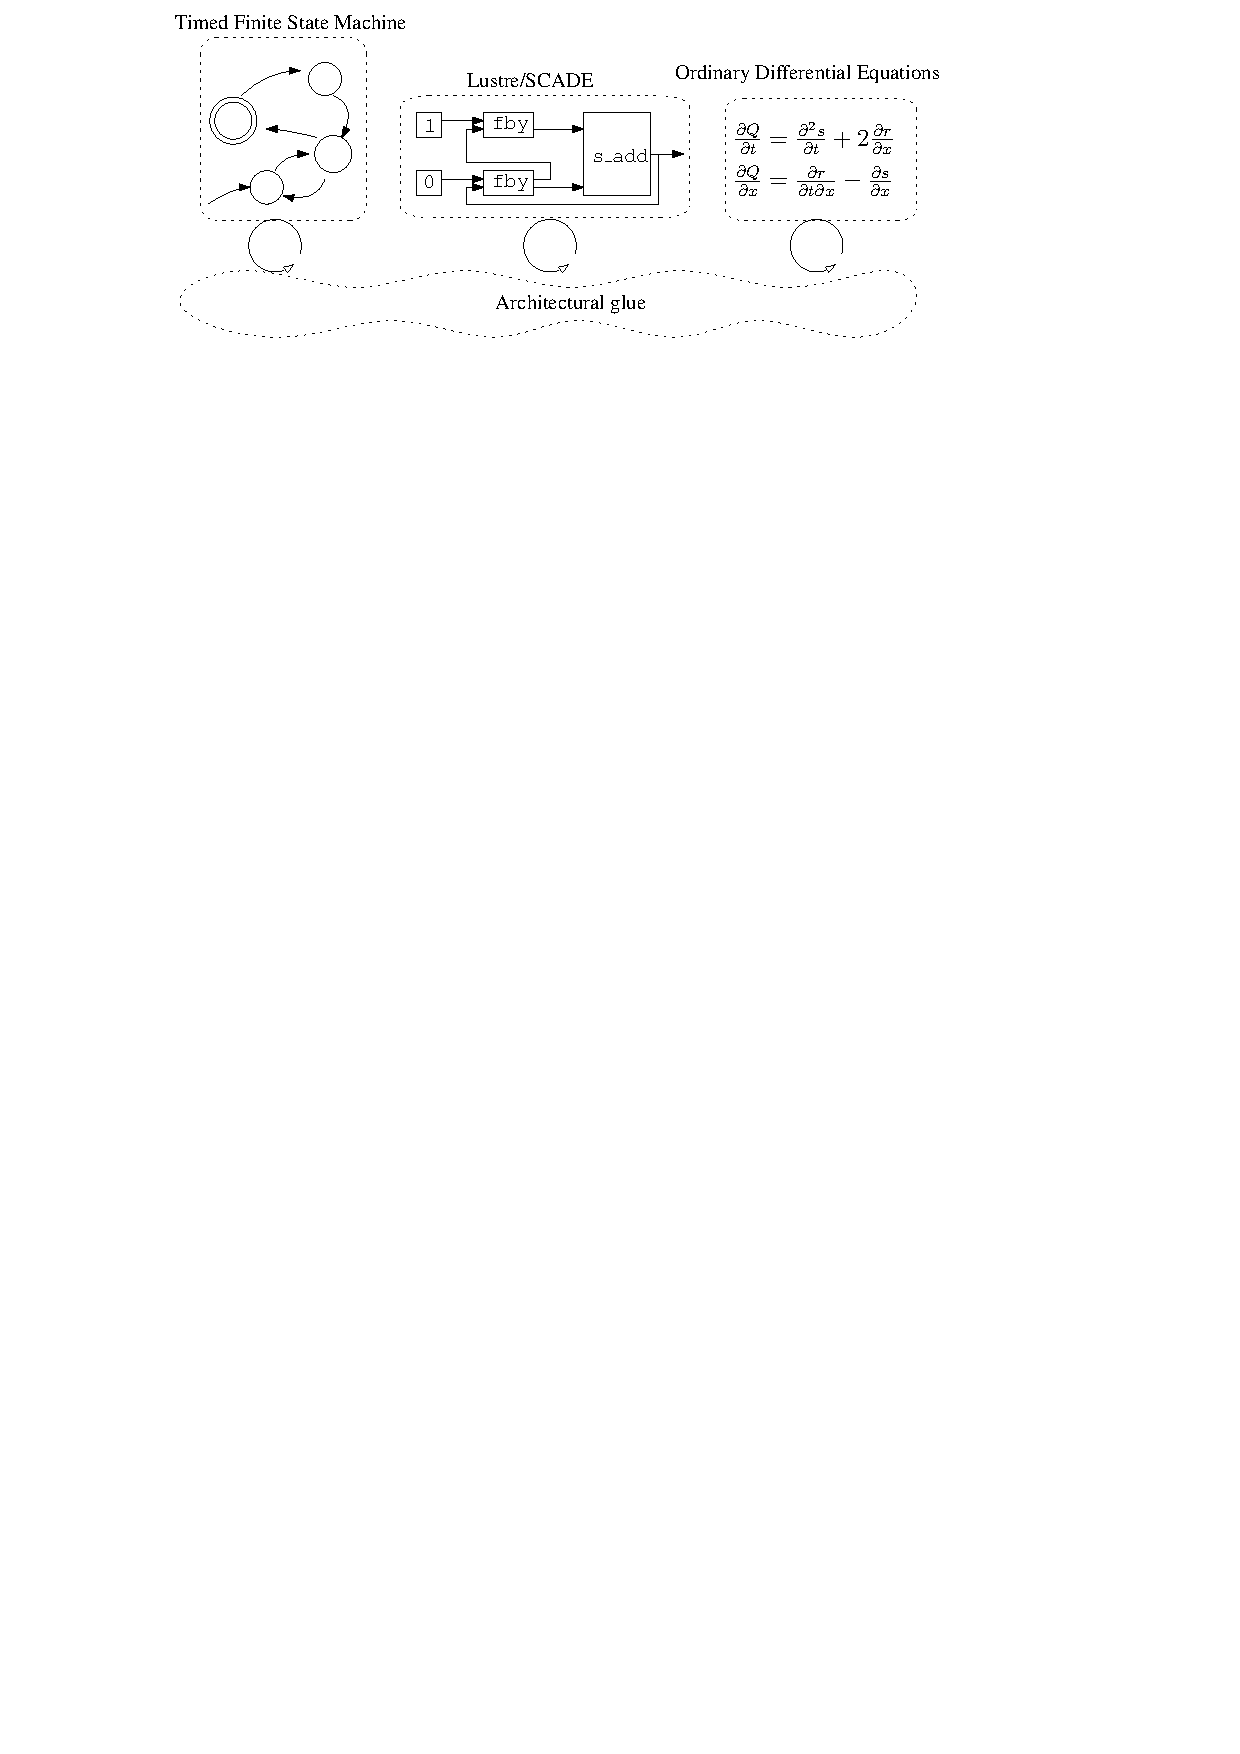
\includegraphics{glue.pdf}
 \caption{A Heterogeneous Timed System Model}
 \label{fig:het-timed-system}
\end{figure}%
\end{isamarkuptext}\isamarkuptrue%
%
\begin{isamarkuptext}%
In order to tackle the heterogeneous nature of the subsystems, we abstract their behavior as clocks. 
Each clock models an event – something that can occur or not at a given time. This time is measured 
in a time frame associated with each clock, and the nature of time (integer, rational, real or any 
type with a linear order) is specific to each clock. 
When the event associated with a clock occurs, the clock ticks. In order to support any kind of 
behavior for the subsystems, we are only interested in specifying what we can observe at a series 
of discrete instants. There are two constraints on observations: a clock may tick only at an 
observation instant, and the time on any clock cannot decrease from an instant to the next one. 
However, it is always possible to add arbitrary observation instants, which allows for stuttering 
and modular composition of systems. 
As a consequence, the key concept of our setting is the notion of a clock-indexed Kripke model: 
\isa{{\isasymSigma}\isactrlsup {\isasyminfinity}\ {\isacharequal}\ {\isasymnat}\ {\isasymrightarrow}\ {\isasymK}\ {\isasymrightarrow}\ {\isacharparenleft}{\isasymbool}\ {\isasymtimes}\ {\isasymT}{\isacharparenright}}, where \isa{{\isasymK}} is an enumerable set of clocks, \isa{{\isasymbool}} 
is the set of booleans – used to  indicate that a clock ticks at a given instant – and \isa{{\isasymT}} 
is a universal metric time space for which we only assume that it is large enough to contain all 
individual time spaces of clocks and that it is ordered by some linear ordering \isa{{\isacharparenleft}{\isasymle}\isactrlsub {\isasymT}{\isacharparenright}}.%
\end{isamarkuptext}\isamarkuptrue%
%
\begin{isamarkuptext}%
The elements of \isa{{\isasymSigma}\isactrlsup {\isasyminfinity}} are called runs. A specification language is a set of 
  operators that constrains the set of possible monotonic runs. Specifications are composed by 
  intersecting the denoted run sets of constraint operators.
  Consequently, such specification languages do not limit the number of clocks used to model a 
  system (as long as it is finite) and it is always possible to add clocks to a specification. 
  Moreover they are \emph{compositional} by construction since the composition of specifications 
  consists of the conjunction of their constraints.%
\end{isamarkuptext}\isamarkuptrue%
%
\begin{isamarkuptext}%
This work provides the following contributions:

%
\begin{itemize}%
\item defining the non-trivial language \isa{TESL\isactrlsup {\isacharasterisk}} in terms of clock-indexed Kripke models, 

\item proving that this denotational semantics is stuttering invariant,

\item defining an adapted form of symbolic primitives and presenting the set of operational 
semantic rules,

\item presenting formal proofs for soundness, completeness, and progress of the latter.%
\end{itemize}%
\end{isamarkuptext}\isamarkuptrue%
%
\isadelimdocument
%
\endisadelimdocument
%
\isatagdocument
%
\isamarkupsection{The TESL Language%
}
\isamarkuptrue%
%
\endisatagdocument
{\isafolddocument}%
%
\isadelimdocument
%
\endisadelimdocument
%
\begin{isamarkuptext}%
The TESL language \cite{BouJacHarPro2014MEMOCODE} was initially designed to coordinate the
  execution of heterogeneous components during the simulation of a system. We define here a minimal
  kernel of operators that will form the basis of a family of specification languages, including the
  original TESL language, which is described at \url{http://wdi.supelec.fr/software/TESL/}.%
\end{isamarkuptext}\isamarkuptrue%
%
\isadelimdocument
%
\endisadelimdocument
%
\isatagdocument
%
\isamarkupsubsection{Instantaneous Causal Operators%
}
\isamarkuptrue%
%
\endisatagdocument
{\isafolddocument}%
%
\isadelimdocument
%
\endisadelimdocument
%
\begin{isamarkuptext}%
TESL has operators to deal with instantaneous causality, i.e. to react to an event occurrence
in the very same observation instant.

%
\begin{itemize}%
\item \isatt{c1\ implies\ c2} means that at any instant where \isatt{c1} ticks, \isatt{c2} has to tick too.

\item \isatt{c1\ implies\ not\ c2} means that at any instant where \isatt{c1} ticks, \isatt{c2} cannot tick.

\item \isatt{c1\ kills\ c2} means that at any instant where \isatt{c1} ticks, and at any future instant, 
\isatt{c2} cannot tick.%
\end{itemize}%
\end{isamarkuptext}\isamarkuptrue%
%
\isadelimdocument
%
\endisadelimdocument
%
\isatagdocument
%
\isamarkupsubsection{Temporal Operators%
}
\isamarkuptrue%
%
\endisatagdocument
{\isafolddocument}%
%
\isadelimdocument
%
\endisadelimdocument
%
\begin{isamarkuptext}%
TESL also has chronometric temporal operators that deal with dates and chronometric delays.

%
\begin{itemize}%
\item \isatt{c\ sporadic\ t} means that clock \isatt{c} must have a tick at time \isatt{t} on its own time scale.

\item \isatt{c1\ sporadic\ t\ on\ c2} means that clock \isatt{c1} must have a tick at an instant where the time 
on \isatt{c2} is \isatt{t}.

\item \isatt{c1\ time\ delayed\ by\ d\ on\ m\ implies\ c2} means that every time clock \isatt{c1} ticks, \isatt{c2} must have 
a tick at the first instant where the time on \isatt{m} is \isatt{d} later than it was when \isatt{c1} had ticked.
This means that every tick on \isatt{c1} is followed by a tick on \isatt{c2} after a delay \isatt{d} measured
on the time scale of closk \isatt{m}.

\item \isatt{time\ relation\ (c1{\char`\,}\ c2)\ in\ R} means that at every instant, the current times on clocks \isatt{c1}
and \isatt{c2} must be in relation \isatt{R}. By default, the time lines of different clocks are 
independent. This operator allows us to link two time lines, for instance to model the fact
that time in a GPS satellite and time in a GPS receiver on Earth are not the same but are 
related. Time being polymorphic in TESL, this can also be used to model the fact that the
angular position on the camshaft of an engine moves twice as fast as the angular position 
on the crankshaft~\footnote{See \url{http://wdi.supelec.fr/software/TESL/GalleryEngine} for more details}. 
We will consider only linear relations here so that finding solutions is decidable.%
\end{itemize}%
\end{isamarkuptext}\isamarkuptrue%
%
\isadelimdocument
%
\endisadelimdocument
%
\isatagdocument
%
\isamarkupsubsection{Asynchronous Operators%
}
\isamarkuptrue%
%
\endisatagdocument
{\isafolddocument}%
%
\isadelimdocument
%
\endisadelimdocument
%
\begin{isamarkuptext}%
The last category of TESL operators allows the specification of asynchronous relations between
event occurrences. They do not tell when ticks have to occur, then only put bounds on the set 
of instants at which they should occur.

%
\begin{itemize}%
\item \isatt{c1\ weakly\ precedes\ c2} means that for each tick on \isatt{c2}, there must be at least one tick
on \isatt{c1} at a previous instant or at the same instant. This can also be expressed by saying
that at each instant, the number of ticks on \isatt{c2} since the beginning of the run must be lower 
or equal to the number of ticks on \isatt{c1}.

\item \isatt{c1\ strictly\ precedes\ c2} means that for each tick on \isatt{c2}, there must be at least one tick
on \isatt{c1} at a previous instant. This can also be expressed by saying that at each instant, 
the number of ticks on \isatt{c2} from the beginning of the run to this instant must be lower or 
equal to the number of ticks on \isatt{c1} from the beginning of the run to the previous instant.%
\end{itemize}%
\end{isamarkuptext}\isamarkuptrue%
%
\isadelimtheory
%
\endisadelimtheory
%
\isatagtheory
%
\endisatagtheory
{\isafoldtheory}%
%
\isadelimtheory
%
\endisadelimtheory
%
\end{isabellebody}%
\endinput
%:%file=~/Documents/Recherche/Thesards/2014_Hai_NGUYEN_VAN/Heron_git/reiher2/reiher/src/Introduction.thy%:%
%:%11=1%:%
%:%41=10%:%
%:%53=12%:%
%:%54=13%:%
%:%55=14%:%
%:%56=15%:%
%:%57=16%:%
%:%58=17%:%
%:%59=18%:%
%:%60=19%:%
%:%62=21%:%
%:%63=22%:%
%:%67=23%:%
%:%68=24%:%
%:%70=25%:%
%:%71=26%:%
%:%73=27%:%
%:%74=28%:%
%:%76=29%:%
%:%77=30%:%
%:%78=31%:%
%:%80=32%:%
%:%81=33%:%
%:%83=34%:%
%:%84=35%:%
%:%89=39%:%
%:%90=40%:%
%:%91=41%:%
%:%92=42%:%
%:%93=43%:%
%:%94=44%:%
%:%98=66%:%
%:%99=67%:%
%:%100=68%:%
%:%101=69%:%
%:%102=70%:%
%:%103=71%:%
%:%104=72%:%
%:%105=73%:%
%:%106=74%:%
%:%107=75%:%
%:%108=76%:%
%:%109=77%:%
%:%110=78%:%
%:%111=79%:%
%:%112=80%:%
%:%116=84%:%
%:%117=85%:%
%:%118=86%:%
%:%119=87%:%
%:%120=88%:%
%:%121=89%:%
%:%122=90%:%
%:%126=94%:%
%:%130=95%:%
%:%132=96%:%
%:%134=97%:%
%:%135=98%:%
%:%137=99%:%
%:%147=102%:%
%:%159=105%:%
%:%160=106%:%
%:%161=107%:%
%:%162=108%:%
%:%171=111%:%
%:%183=113%:%
%:%184=114%:%
%:%188=115%:%
%:%190=116%:%
%:%192=117%:%
%:%193=118%:%
%:%203=121%:%
%:%215=123%:%
%:%219=124%:%
%:%221=125%:%
%:%222=126%:%
%:%224=127%:%
%:%225=128%:%
%:%226=129%:%
%:%227=130%:%
%:%229=131%:%
%:%230=132%:%
%:%231=133%:%
%:%232=134%:%
%:%233=135%:%
%:%234=136%:%
%:%235=137%:%
%:%236=138%:%
%:%246=141%:%
%:%258=143%:%
%:%259=144%:%
%:%260=145%:%
%:%264=146%:%
%:%265=147%:%
%:%266=148%:%
%:%267=149%:%
%:%269=150%:%
%:%270=151%:%
%:%271=152%:%
%:%272=153%:%

%
\begin{isabellebody}%
\setisabellecontext{TESL}%
%
\begin{isamarkuptext}%
\chapter[Core TESL: Syntax and Basics]{The Core of the TESL Language: Syntax and Basics}%
\end{isamarkuptext}\isamarkuptrue%
%
\isadelimtheory
%
\endisadelimtheory
%
\isatagtheory
\isacommand{theory}\isamarkupfalse%
\ TESL\isanewline
\isakeyword{imports}\ Main\isanewline
\isanewline
\isakeyword{begin}%
\endisatagtheory
{\isafoldtheory}%
%
\isadelimtheory
%
\endisadelimtheory
%
\isadelimdocument
%
\endisadelimdocument
%
\isatagdocument
%
\isamarkupsection{Syntactic Representation%
}
\isamarkuptrue%
%
\endisatagdocument
{\isafolddocument}%
%
\isadelimdocument
%
\endisadelimdocument
%
\begin{isamarkuptext}%
We define here the syntax of TESL specifications.%
\end{isamarkuptext}\isamarkuptrue%
%
\isadelimdocument
%
\endisadelimdocument
%
\isatagdocument
%
\isamarkupsubsection{Basic elements of a specification%
}
\isamarkuptrue%
%
\endisatagdocument
{\isafolddocument}%
%
\isadelimdocument
%
\endisadelimdocument
%
\begin{isamarkuptext}%
The following items appear in specifications:

%
\begin{itemize}%
\item Clocks, which are identified by a name.

\item Tag constants are just constants of a type which denotes the metric time space.%
\end{itemize}%
\end{isamarkuptext}\isamarkuptrue%
\isacommand{datatype}\isamarkupfalse%
\ \ \ \ \ clock\ \ \ \ \ \ \ \ \ {\isacharequal}\ Clk\ {\isacartoucheopen}string{\isacartoucheclose}\isanewline
\isacommand{type{\isacharunderscore}synonym}\isamarkupfalse%
\ instant{\isacharunderscore}index\ {\isacharequal}\ {\isacartoucheopen}nat{\isacartoucheclose}\isanewline
\isanewline
\isacommand{datatype}\isamarkupfalse%
\ \ \ \ \ {\isacharprime}{\isasymtau}\ tag{\isacharunderscore}const\ {\isacharequal}\ \ TConst\ \ \ {\isacharparenleft}the{\isacharunderscore}tag{\isacharunderscore}const\ {\isacharcolon}\ {\isacharprime}{\isasymtau}{\isacharparenright}\ \ \ \ \ \ \ \ \ {\isacharparenleft}{\isachardoublequoteopen}{\isasymtau}\isactrlsub c\isactrlsub s\isactrlsub t{\isachardoublequoteclose}{\isacharparenright}%
\isadelimdocument
%
\endisadelimdocument
%
\isatagdocument
%
\isamarkupsubsection{Operators for the TESL language%
}
\isamarkuptrue%
%
\endisatagdocument
{\isafolddocument}%
%
\isadelimdocument
%
\endisadelimdocument
%
\begin{isamarkuptext}%
The type of atomic TESL constraints, which can be combined to form specifications.%
\end{isamarkuptext}\isamarkuptrue%
\isacommand{datatype}\isamarkupfalse%
\ {\isacharprime}{\isasymtau}\ TESL{\isacharunderscore}atomic\ {\isacharequal}\isanewline
\ \ \ \ SporadicOn\ \ \ \ \ \ \ {\isacartoucheopen}clock{\isacartoucheclose}\ {\isacartoucheopen}{\isacharprime}{\isasymtau}\ tag{\isacharunderscore}const{\isacartoucheclose}\ \ {\isacartoucheopen}clock{\isacartoucheclose}\ \ {\isacharparenleft}{\isachardoublequoteopen}{\isacharunderscore}\ sporadic\ {\isacharunderscore}\ on\ {\isacharunderscore}{\isachardoublequoteclose}\ {\isadigit{5}}{\isadigit{5}}{\isacharparenright}\isanewline
\ \ {\isacharbar}\ TagRelation\ \ \ \ \ \ {\isacartoucheopen}clock{\isacartoucheclose}\ {\isacartoucheopen}clock{\isacartoucheclose}\ {\isacartoucheopen}{\isacharparenleft}{\isacharprime}{\isasymtau}\ tag{\isacharunderscore}const\ {\isasymtimes}\ {\isacharprime}{\isasymtau}\ tag{\isacharunderscore}const{\isacharparenright}\ {\isasymRightarrow}\ bool{\isacartoucheclose}\ \isanewline
\ \ \ \ \ \ \ \ \ \ \ \ \ \ \ \ \ \ \ \ \ \ \ \ \ \ \ \ \ \ \ \ \ \ \ \ \ \ \ \ \ \ \ \ \ \ \ \ \ \ \ \ \ \ {\isacharparenleft}{\isachardoublequoteopen}time{\isacharminus}relation\ {\isasymlfloor}{\isacharunderscore}{\isacharcomma}\ {\isacharunderscore}{\isasymrfloor}\ {\isasymin}\ {\isacharunderscore}{\isachardoublequoteclose}\ {\isadigit{5}}{\isadigit{5}}{\isacharparenright}\isanewline
\ \ {\isacharbar}\ Implies\ \ \ \ \ \ \ \ \ \ {\isacartoucheopen}clock{\isacartoucheclose}\ {\isacartoucheopen}clock{\isacartoucheclose}\ \ \ \ \ \ \ \ \ \ \ \ \ \ \ \ \ \ {\isacharparenleft}\isakeyword{infixr}\ {\isachardoublequoteopen}implies{\isachardoublequoteclose}\ {\isadigit{5}}{\isadigit{5}}{\isacharparenright}\isanewline
\ \ {\isacharbar}\ ImpliesNot\ \ \ \ \ \ \ {\isacartoucheopen}clock{\isacartoucheclose}\ {\isacartoucheopen}clock{\isacartoucheclose}\ \ \ \ \ \ \ \ \ \ \ \ \ \ \ \ \ \ {\isacharparenleft}\isakeyword{infixr}\ {\isachardoublequoteopen}implies\ not{\isachardoublequoteclose}\ {\isadigit{5}}{\isadigit{5}}{\isacharparenright}\isanewline
\ \ {\isacharbar}\ TimeDelayedBy\ \ \ \ {\isacartoucheopen}clock{\isacartoucheclose}\ {\isacartoucheopen}{\isacharprime}{\isasymtau}\ tag{\isacharunderscore}const{\isacartoucheclose}\ {\isacartoucheopen}clock{\isacartoucheclose}\ {\isacartoucheopen}clock{\isacartoucheclose}\ \isanewline
\ \ \ \ \ \ \ \ \ \ \ \ \ \ \ \ \ \ \ \ \ \ \ \ \ \ \ \ \ \ \ \ \ \ \ \ \ \ \ \ \ \ \ \ \ \ \ \ \ \ \ \ \ \ {\isacharparenleft}{\isachardoublequoteopen}{\isacharunderscore}\ time{\isacharminus}delayed\ by\ {\isacharunderscore}\ on\ {\isacharunderscore}\ implies\ {\isacharunderscore}{\isachardoublequoteclose}\ {\isadigit{5}}{\isadigit{5}}{\isacharparenright}\isanewline
\ \ {\isacharbar}\ WeaklyPrecedes\ \ \ {\isacartoucheopen}clock{\isacartoucheclose}\ {\isacartoucheopen}clock{\isacartoucheclose}\ \ \ \ \ \ \ \ \ \ \ \ \ \ \ \ \ \ {\isacharparenleft}\isakeyword{infixr}\ {\isachardoublequoteopen}weakly\ precedes{\isachardoublequoteclose}\ {\isadigit{5}}{\isadigit{5}}{\isacharparenright}\isanewline
\ \ {\isacharbar}\ StrictlyPrecedes\ {\isacartoucheopen}clock{\isacartoucheclose}\ {\isacartoucheopen}clock{\isacartoucheclose}\ \ \ \ \ \ \ \ \ \ \ \ \ \ \ \ \ \ {\isacharparenleft}\isakeyword{infixr}\ {\isachardoublequoteopen}strictly\ precedes{\isachardoublequoteclose}\ {\isadigit{5}}{\isadigit{5}}{\isacharparenright}\isanewline
\ \ {\isacharbar}\ Kills\ \ \ \ \ \ \ \ \ \ \ \ {\isacartoucheopen}clock{\isacartoucheclose}\ {\isacartoucheopen}clock{\isacartoucheclose}\ \ \ \ \ \ \ \ \ \ \ \ \ \ \ \ \ \ {\isacharparenleft}\isakeyword{infixr}\ {\isachardoublequoteopen}kills{\isachardoublequoteclose}\ {\isadigit{5}}{\isadigit{5}}{\isacharparenright}%
\begin{isamarkuptext}%
A TESL formula is just a list of atomic constraints, with implicit conjunction
  for the semantics.%
\end{isamarkuptext}\isamarkuptrue%
\isacommand{type{\isacharunderscore}synonym}\isamarkupfalse%
\ {\isacharprime}{\isasymtau}\ TESL{\isacharunderscore}formula\ {\isacharequal}\ {\isacartoucheopen}{\isacharprime}{\isasymtau}\ TESL{\isacharunderscore}atomic\ list{\isacartoucheclose}%
\begin{isamarkuptext}%
We call \emph{positive atoms} the atomic constraints that create ticks from nothing.
  Only sporadic constraints are positive in the current version of TESL.%
\end{isamarkuptext}\isamarkuptrue%
\isacommand{fun}\isamarkupfalse%
\ positive{\isacharunderscore}atom\ {\isacharcolon}{\isacharcolon}\ {\isacartoucheopen}{\isacharprime}{\isasymtau}\ TESL{\isacharunderscore}atomic\ {\isasymRightarrow}\ bool{\isacartoucheclose}\ \isakeyword{where}\isanewline
\ \ \ \ {\isacartoucheopen}positive{\isacharunderscore}atom\ {\isacharparenleft}{\isacharunderscore}\ sporadic\ {\isacharunderscore}\ on\ {\isacharunderscore}{\isacharparenright}\ {\isacharequal}\ True{\isacartoucheclose}\isanewline
\ \ {\isacharbar}\ {\isacartoucheopen}positive{\isacharunderscore}atom\ {\isacharunderscore}\ \ \ \ \ \ \ \ \ \ \ \ \ \ \ \ \ \ \ {\isacharequal}\ False{\isacartoucheclose}%
\begin{isamarkuptext}%
The \isa{NoSporadic} function removes sporadic constraints from a TESL formula.%
\end{isamarkuptext}\isamarkuptrue%
\isacommand{abbreviation}\isamarkupfalse%
\ NoSporadic\ {\isacharcolon}{\isacharcolon}\ {\isacartoucheopen}{\isacharprime}{\isasymtau}\ TESL{\isacharunderscore}formula\ {\isasymRightarrow}\ {\isacharprime}{\isasymtau}\ TESL{\isacharunderscore}formula{\isacartoucheclose}\isanewline
\isakeyword{where}\ \isanewline
\ \ {\isacartoucheopen}NoSporadic\ f\ {\isasymequiv}\ {\isacharparenleft}List{\isachardot}filter\ {\isacharparenleft}{\isasymlambda}f\isactrlsub a\isactrlsub t\isactrlsub o\isactrlsub m{\isachardot}\ case\ f\isactrlsub a\isactrlsub t\isactrlsub o\isactrlsub m\ of\isanewline
\ \ \ \ \ \ {\isacharunderscore}\ sporadic\ {\isacharunderscore}\ on\ {\isacharunderscore}\ {\isasymRightarrow}\ False\isanewline
\ \ \ \ {\isacharbar}\ {\isacharunderscore}\ {\isasymRightarrow}\ True{\isacharparenright}\ f{\isacharparenright}{\isacartoucheclose}%
\isadelimdocument
%
\endisadelimdocument
%
\isatagdocument
%
\isamarkupsubsection{Field Structure of the Metric Time Space%
}
\isamarkuptrue%
%
\endisatagdocument
{\isafolddocument}%
%
\isadelimdocument
%
\endisadelimdocument
%
\begin{isamarkuptext}%
In order to handle tag relations and delays, tags must belong to a field.
  We show here that this is the case when the type parameter of \isa{{\isacharprime}{\isasymtau}\ tag{\isacharunderscore}const} 
  is itself a field.%
\end{isamarkuptext}\isamarkuptrue%
\isacommand{instantiation}\isamarkupfalse%
\ tag{\isacharunderscore}const\ {\isacharcolon}{\isacharcolon}{\isacharparenleft}field{\isacharparenright}field\isanewline
\isakeyword{begin}\isanewline
\ \ \isacommand{fun}\isamarkupfalse%
\ inverse{\isacharunderscore}tag{\isacharunderscore}const\isanewline
\ \ \isakeyword{where}\ {\isacartoucheopen}inverse\ {\isacharparenleft}{\isasymtau}\isactrlsub c\isactrlsub s\isactrlsub t\ t{\isacharparenright}\ {\isacharequal}\ {\isasymtau}\isactrlsub c\isactrlsub s\isactrlsub t\ {\isacharparenleft}inverse\ t{\isacharparenright}{\isacartoucheclose}\isanewline
\isanewline
\ \ \isacommand{fun}\isamarkupfalse%
\ divide{\isacharunderscore}tag{\isacharunderscore}const\ \isanewline
\ \ \ \ \isakeyword{where}\ {\isacartoucheopen}divide\ {\isacharparenleft}{\isasymtau}\isactrlsub c\isactrlsub s\isactrlsub t\ t\isactrlsub {\isadigit{1}}{\isacharparenright}\ {\isacharparenleft}{\isasymtau}\isactrlsub c\isactrlsub s\isactrlsub t\ t\isactrlsub {\isadigit{2}}{\isacharparenright}\ {\isacharequal}\ {\isasymtau}\isactrlsub c\isactrlsub s\isactrlsub t\ {\isacharparenleft}divide\ t\isactrlsub {\isadigit{1}}\ t\isactrlsub {\isadigit{2}}{\isacharparenright}{\isacartoucheclose}\isanewline
\isanewline
\ \ \isacommand{fun}\isamarkupfalse%
\ uminus{\isacharunderscore}tag{\isacharunderscore}const\isanewline
\ \ \ \ \isakeyword{where}\ {\isacartoucheopen}uminus\ {\isacharparenleft}{\isasymtau}\isactrlsub c\isactrlsub s\isactrlsub t\ t{\isacharparenright}\ {\isacharequal}\ {\isasymtau}\isactrlsub c\isactrlsub s\isactrlsub t\ {\isacharparenleft}uminus\ t{\isacharparenright}{\isacartoucheclose}\isanewline
\isanewline
\isacommand{fun}\isamarkupfalse%
\ minus{\isacharunderscore}tag{\isacharunderscore}const\isanewline
\ \ \isakeyword{where}\ {\isacartoucheopen}minus\ {\isacharparenleft}{\isasymtau}\isactrlsub c\isactrlsub s\isactrlsub t\ t\isactrlsub {\isadigit{1}}{\isacharparenright}\ {\isacharparenleft}{\isasymtau}\isactrlsub c\isactrlsub s\isactrlsub t\ t\isactrlsub {\isadigit{2}}{\isacharparenright}\ {\isacharequal}\ {\isasymtau}\isactrlsub c\isactrlsub s\isactrlsub t\ {\isacharparenleft}minus\ t\isactrlsub {\isadigit{1}}\ t\isactrlsub {\isadigit{2}}{\isacharparenright}{\isacartoucheclose}\isanewline
\isanewline
\isacommand{definition}\isamarkupfalse%
\ {\isacartoucheopen}one{\isacharunderscore}tag{\isacharunderscore}const\ {\isasymequiv}\ {\isasymtau}\isactrlsub c\isactrlsub s\isactrlsub t\ {\isadigit{1}}{\isacartoucheclose}\isanewline
\isanewline
\isacommand{fun}\isamarkupfalse%
\ times{\isacharunderscore}tag{\isacharunderscore}const\isanewline
\ \ \isakeyword{where}\ {\isacartoucheopen}times\ {\isacharparenleft}{\isasymtau}\isactrlsub c\isactrlsub s\isactrlsub t\ t\isactrlsub {\isadigit{1}}{\isacharparenright}\ {\isacharparenleft}{\isasymtau}\isactrlsub c\isactrlsub s\isactrlsub t\ t\isactrlsub {\isadigit{2}}{\isacharparenright}\ {\isacharequal}\ {\isasymtau}\isactrlsub c\isactrlsub s\isactrlsub t\ {\isacharparenleft}times\ t\isactrlsub {\isadigit{1}}\ t\isactrlsub {\isadigit{2}}{\isacharparenright}{\isacartoucheclose}\isanewline
\isanewline
\isacommand{definition}\isamarkupfalse%
\ {\isacartoucheopen}zero{\isacharunderscore}tag{\isacharunderscore}const\ {\isasymequiv}\ {\isasymtau}\isactrlsub c\isactrlsub s\isactrlsub t\ {\isadigit{0}}{\isacartoucheclose}\isanewline
\isanewline
\isacommand{fun}\isamarkupfalse%
\ plus{\isacharunderscore}tag{\isacharunderscore}const\isanewline
\ \ \isakeyword{where}\ {\isacartoucheopen}plus\ {\isacharparenleft}{\isasymtau}\isactrlsub c\isactrlsub s\isactrlsub t\ t\isactrlsub {\isadigit{1}}{\isacharparenright}\ {\isacharparenleft}{\isasymtau}\isactrlsub c\isactrlsub s\isactrlsub t\ t\isactrlsub {\isadigit{2}}{\isacharparenright}\ {\isacharequal}\ {\isasymtau}\isactrlsub c\isactrlsub s\isactrlsub t\ {\isacharparenleft}plus\ t\isactrlsub {\isadigit{1}}\ t\isactrlsub {\isadigit{2}}{\isacharparenright}{\isacartoucheclose}\isanewline
\isanewline
\isacommand{instance}\isamarkupfalse%
%
\isadelimproof
\ %
\endisadelimproof
%
\isatagproof
\isacommand{proof}\isamarkupfalse%
%
\begin{isamarkuptext}%
Multiplication is associative.%
\end{isamarkuptext}\isamarkuptrue%
\ \ \isacommand{fix}\isamarkupfalse%
\ a{\isacharcolon}{\isacharcolon}{\isacartoucheopen}{\isacharprime}{\isasymtau}{\isacharcolon}{\isacharcolon}field\ tag{\isacharunderscore}const{\isacartoucheclose}\ \isakeyword{and}\ b{\isacharcolon}{\isacharcolon}{\isacartoucheopen}{\isacharprime}{\isasymtau}{\isacharcolon}{\isacharcolon}field\ tag{\isacharunderscore}const{\isacartoucheclose}\isanewline
\ \ \ \ \ \ \ \ \ \ \ \ \ \ \ \ \ \ \ \ \ \ \ \ \ \ \ \ \ \ \ \isakeyword{and}\ c{\isacharcolon}{\isacharcolon}{\isacartoucheopen}{\isacharprime}{\isasymtau}{\isacharcolon}{\isacharcolon}field\ tag{\isacharunderscore}const{\isacartoucheclose}\isanewline
\ \ \isacommand{obtain}\isamarkupfalse%
\ u\ v\ w\ \isakeyword{where}\ {\isacartoucheopen}a\ {\isacharequal}\ {\isasymtau}\isactrlsub c\isactrlsub s\isactrlsub t\ u{\isacartoucheclose}\ \isakeyword{and}\ {\isacartoucheopen}b\ {\isacharequal}\ {\isasymtau}\isactrlsub c\isactrlsub s\isactrlsub t\ v{\isacartoucheclose}\ \isakeyword{and}\ {\isacartoucheopen}c\ {\isacharequal}\ {\isasymtau}\isactrlsub c\isactrlsub s\isactrlsub t\ w{\isacartoucheclose}\isanewline
\ \ \ \ \isacommand{using}\isamarkupfalse%
\ tag{\isacharunderscore}const{\isachardot}exhaust\ \isacommand{by}\isamarkupfalse%
\ metis\isanewline
\ \ \isacommand{thus}\isamarkupfalse%
\ {\isacartoucheopen}a\ {\isacharasterisk}\ b\ {\isacharasterisk}\ c\ {\isacharequal}\ a\ {\isacharasterisk}\ {\isacharparenleft}b\ {\isacharasterisk}\ c{\isacharparenright}{\isacartoucheclose}\isanewline
\ \ \ \ \isacommand{by}\isamarkupfalse%
\ {\isacharparenleft}simp\ add{\isacharcolon}\ TESL{\isachardot}times{\isacharunderscore}tag{\isacharunderscore}const{\isachardot}simps{\isacharparenright}\isanewline
\isacommand{next}\isamarkupfalse%
%
\begin{isamarkuptext}%
Multiplication is commutative.%
\end{isamarkuptext}\isamarkuptrue%
\ \ \isacommand{fix}\isamarkupfalse%
\ a{\isacharcolon}{\isacharcolon}{\isacartoucheopen}{\isacharprime}{\isasymtau}{\isacharcolon}{\isacharcolon}field\ tag{\isacharunderscore}const{\isacartoucheclose}\ \isakeyword{and}\ b{\isacharcolon}{\isacharcolon}{\isacartoucheopen}{\isacharprime}{\isasymtau}{\isacharcolon}{\isacharcolon}field\ tag{\isacharunderscore}const{\isacartoucheclose}\isanewline
\ \ \isacommand{obtain}\isamarkupfalse%
\ u\ v\ \isakeyword{where}\ {\isacartoucheopen}a\ {\isacharequal}\ {\isasymtau}\isactrlsub c\isactrlsub s\isactrlsub t\ u{\isacartoucheclose}\ \isakeyword{and}\ {\isacartoucheopen}b\ {\isacharequal}\ {\isasymtau}\isactrlsub c\isactrlsub s\isactrlsub t\ v{\isacartoucheclose}\ \isacommand{using}\isamarkupfalse%
\ tag{\isacharunderscore}const{\isachardot}exhaust\ \isacommand{by}\isamarkupfalse%
\ metis\isanewline
\ \ \isacommand{thus}\isamarkupfalse%
\ {\isacartoucheopen}\ a\ {\isacharasterisk}\ b\ {\isacharequal}\ b\ {\isacharasterisk}\ a{\isacartoucheclose}\isanewline
\ \ \ \ \isacommand{by}\isamarkupfalse%
\ {\isacharparenleft}simp\ add{\isacharcolon}\ TESL{\isachardot}times{\isacharunderscore}tag{\isacharunderscore}const{\isachardot}simps{\isacharparenright}\isanewline
\isacommand{next}\isamarkupfalse%
%
\begin{isamarkuptext}%
One is neutral for multiplication.%
\end{isamarkuptext}\isamarkuptrue%
\ \ \isacommand{fix}\isamarkupfalse%
\ a{\isacharcolon}{\isacharcolon}{\isacartoucheopen}{\isacharprime}{\isasymtau}{\isacharcolon}{\isacharcolon}field\ tag{\isacharunderscore}const{\isacartoucheclose}\isanewline
\ \ \isacommand{obtain}\isamarkupfalse%
\ u\ \isakeyword{where}\ {\isacartoucheopen}a\ {\isacharequal}\ {\isasymtau}\isactrlsub c\isactrlsub s\isactrlsub t\ u{\isacartoucheclose}\ \isacommand{using}\isamarkupfalse%
\ tag{\isacharunderscore}const{\isachardot}exhaust\ \isacommand{by}\isamarkupfalse%
\ blast\isanewline
\ \ \isacommand{thus}\isamarkupfalse%
\ {\isacartoucheopen}{\isadigit{1}}\ {\isacharasterisk}\ a\ {\isacharequal}\ a{\isacartoucheclose}\isanewline
\ \ \ \ \isacommand{by}\isamarkupfalse%
\ {\isacharparenleft}simp\ add{\isacharcolon}\ TESL{\isachardot}times{\isacharunderscore}tag{\isacharunderscore}const{\isachardot}simps\ one{\isacharunderscore}tag{\isacharunderscore}const{\isacharunderscore}def{\isacharparenright}\isanewline
\isacommand{next}\isamarkupfalse%
%
\begin{isamarkuptext}%
Addition is associative.%
\end{isamarkuptext}\isamarkuptrue%
\ \ \isacommand{fix}\isamarkupfalse%
\ a{\isacharcolon}{\isacharcolon}{\isacartoucheopen}{\isacharprime}{\isasymtau}{\isacharcolon}{\isacharcolon}field\ tag{\isacharunderscore}const{\isacartoucheclose}\ \isakeyword{and}\ b{\isacharcolon}{\isacharcolon}{\isacartoucheopen}{\isacharprime}{\isasymtau}{\isacharcolon}{\isacharcolon}field\ tag{\isacharunderscore}const{\isacartoucheclose}\isanewline
\ \ \ \ \ \ \ \ \ \ \ \ \ \ \ \ \ \ \ \ \ \ \ \ \ \ \ \ \ \ \ \isakeyword{and}\ c{\isacharcolon}{\isacharcolon}{\isacartoucheopen}{\isacharprime}{\isasymtau}{\isacharcolon}{\isacharcolon}field\ tag{\isacharunderscore}const{\isacartoucheclose}\isanewline
\ \ \isacommand{obtain}\isamarkupfalse%
\ u\ v\ w\ \isakeyword{where}\ {\isacartoucheopen}a\ {\isacharequal}\ {\isasymtau}\isactrlsub c\isactrlsub s\isactrlsub t\ u{\isacartoucheclose}\ \isakeyword{and}\ {\isacartoucheopen}b\ {\isacharequal}\ {\isasymtau}\isactrlsub c\isactrlsub s\isactrlsub t\ v{\isacartoucheclose}\ \isakeyword{and}\ {\isacartoucheopen}c\ {\isacharequal}\ {\isasymtau}\isactrlsub c\isactrlsub s\isactrlsub t\ w{\isacartoucheclose}\isanewline
\ \ \ \ \isacommand{using}\isamarkupfalse%
\ tag{\isacharunderscore}const{\isachardot}exhaust\ \isacommand{by}\isamarkupfalse%
\ metis\isanewline
\ \ \isacommand{thus}\isamarkupfalse%
\ {\isacartoucheopen}a\ {\isacharplus}\ b\ {\isacharplus}\ c\ {\isacharequal}\ a\ {\isacharplus}\ {\isacharparenleft}b\ {\isacharplus}\ c{\isacharparenright}{\isacartoucheclose}\isanewline
\ \ \ \ \isacommand{by}\isamarkupfalse%
\ {\isacharparenleft}simp\ add{\isacharcolon}\ TESL{\isachardot}plus{\isacharunderscore}tag{\isacharunderscore}const{\isachardot}simps{\isacharparenright}\isanewline
\isacommand{next}\isamarkupfalse%
%
\begin{isamarkuptext}%
Addition is commutative.%
\end{isamarkuptext}\isamarkuptrue%
\ \ \isacommand{fix}\isamarkupfalse%
\ a{\isacharcolon}{\isacharcolon}{\isacartoucheopen}{\isacharprime}{\isasymtau}{\isacharcolon}{\isacharcolon}field\ tag{\isacharunderscore}const{\isacartoucheclose}\ \isakeyword{and}\ b{\isacharcolon}{\isacharcolon}{\isacartoucheopen}{\isacharprime}{\isasymtau}{\isacharcolon}{\isacharcolon}field\ tag{\isacharunderscore}const{\isacartoucheclose}\isanewline
\ \ \isacommand{obtain}\isamarkupfalse%
\ u\ v\ \isakeyword{where}\ {\isacartoucheopen}a\ {\isacharequal}\ {\isasymtau}\isactrlsub c\isactrlsub s\isactrlsub t\ u{\isacartoucheclose}\ \isakeyword{and}\ {\isacartoucheopen}b\ {\isacharequal}\ {\isasymtau}\isactrlsub c\isactrlsub s\isactrlsub t\ v{\isacartoucheclose}\ \isacommand{using}\isamarkupfalse%
\ tag{\isacharunderscore}const{\isachardot}exhaust\ \isacommand{by}\isamarkupfalse%
\ metis\isanewline
\ \ \isacommand{thus}\isamarkupfalse%
\ {\isacartoucheopen}a\ {\isacharplus}\ b\ {\isacharequal}\ b\ {\isacharplus}\ a{\isacartoucheclose}\isanewline
\ \ \ \ \isacommand{by}\isamarkupfalse%
\ {\isacharparenleft}simp\ add{\isacharcolon}\ TESL{\isachardot}plus{\isacharunderscore}tag{\isacharunderscore}const{\isachardot}simps{\isacharparenright}\isanewline
\isacommand{next}\isamarkupfalse%
%
\begin{isamarkuptext}%
Zero is neutral for addition.%
\end{isamarkuptext}\isamarkuptrue%
\ \ \isacommand{fix}\isamarkupfalse%
\ a{\isacharcolon}{\isacharcolon}{\isacartoucheopen}{\isacharprime}{\isasymtau}{\isacharcolon}{\isacharcolon}field\ tag{\isacharunderscore}const{\isacartoucheclose}\isanewline
\ \ \isacommand{obtain}\isamarkupfalse%
\ u\ \isakeyword{where}\ {\isacartoucheopen}a\ {\isacharequal}\ {\isasymtau}\isactrlsub c\isactrlsub s\isactrlsub t\ u{\isacartoucheclose}\ \isacommand{using}\isamarkupfalse%
\ tag{\isacharunderscore}const{\isachardot}exhaust\ \isacommand{by}\isamarkupfalse%
\ blast\isanewline
\ \ \isacommand{thus}\isamarkupfalse%
\ {\isacartoucheopen}{\isadigit{0}}\ {\isacharplus}\ a\ {\isacharequal}\ a{\isacartoucheclose}\isanewline
\ \ \ \ \isacommand{by}\isamarkupfalse%
\ {\isacharparenleft}simp\ add{\isacharcolon}\ TESL{\isachardot}plus{\isacharunderscore}tag{\isacharunderscore}const{\isachardot}simps\ zero{\isacharunderscore}tag{\isacharunderscore}const{\isacharunderscore}def{\isacharparenright}\isanewline
\isacommand{next}\isamarkupfalse%
%
\begin{isamarkuptext}%
The sum of an element and its opposite is zero.%
\end{isamarkuptext}\isamarkuptrue%
\ \ \isacommand{fix}\isamarkupfalse%
\ a{\isacharcolon}{\isacharcolon}{\isacartoucheopen}{\isacharprime}{\isasymtau}{\isacharcolon}{\isacharcolon}field\ tag{\isacharunderscore}const{\isacartoucheclose}\isanewline
\ \ \isacommand{obtain}\isamarkupfalse%
\ u\ \isakeyword{where}\ {\isacartoucheopen}a\ {\isacharequal}\ {\isasymtau}\isactrlsub c\isactrlsub s\isactrlsub t\ u{\isacartoucheclose}\ \isacommand{using}\isamarkupfalse%
\ tag{\isacharunderscore}const{\isachardot}exhaust\ \isacommand{by}\isamarkupfalse%
\ blast\isanewline
\ \ \isacommand{thus}\isamarkupfalse%
\ {\isacartoucheopen}{\isacharminus}a\ {\isacharplus}\ a\ {\isacharequal}\ {\isadigit{0}}{\isacartoucheclose}\isanewline
\ \ \ \ \isacommand{by}\isamarkupfalse%
\ {\isacharparenleft}simp\ add{\isacharcolon}\ TESL{\isachardot}plus{\isacharunderscore}tag{\isacharunderscore}const{\isachardot}simps\isanewline
\ \ \ \ \ \ \ \ \ \ \ \ \ \ \ \ \ \ TESL{\isachardot}uminus{\isacharunderscore}tag{\isacharunderscore}const{\isachardot}simps\isanewline
\ \ \ \ \ \ \ \ \ \ \ \ \ \ \ \ \ \ zero{\isacharunderscore}tag{\isacharunderscore}const{\isacharunderscore}def{\isacharparenright}\isanewline
\isacommand{next}\isamarkupfalse%
%
\begin{isamarkuptext}%
Subtraction is adding the opposite.%
\end{isamarkuptext}\isamarkuptrue%
\ \ \isacommand{fix}\isamarkupfalse%
\ a{\isacharcolon}{\isacharcolon}{\isacartoucheopen}{\isacharprime}{\isasymtau}{\isacharcolon}{\isacharcolon}field\ tag{\isacharunderscore}const{\isacartoucheclose}\ \isakeyword{and}\ b{\isacharcolon}{\isacharcolon}{\isacartoucheopen}{\isacharprime}{\isasymtau}{\isacharcolon}{\isacharcolon}field\ tag{\isacharunderscore}const{\isacartoucheclose}\isanewline
\ \ \isacommand{obtain}\isamarkupfalse%
\ u\ v\ \isakeyword{where}\ {\isacartoucheopen}a\ {\isacharequal}\ {\isasymtau}\isactrlsub c\isactrlsub s\isactrlsub t\ u{\isacartoucheclose}\ \isakeyword{and}\ {\isacartoucheopen}b\ {\isacharequal}\ {\isasymtau}\isactrlsub c\isactrlsub s\isactrlsub t\ v{\isacartoucheclose}\ \isacommand{using}\isamarkupfalse%
\ tag{\isacharunderscore}const{\isachardot}exhaust\ \isacommand{by}\isamarkupfalse%
\ metis\isanewline
\ \ \isacommand{thus}\isamarkupfalse%
\ {\isacartoucheopen}a\ {\isacharminus}\ b\ {\isacharequal}\ a\ {\isacharplus}\ {\isacharminus}b{\isacartoucheclose}\isanewline
\ \ \ \ \isacommand{by}\isamarkupfalse%
\ {\isacharparenleft}simp\ add{\isacharcolon}\ TESL{\isachardot}minus{\isacharunderscore}tag{\isacharunderscore}const{\isachardot}simps\isanewline
\ \ \ \ \ \ \ \ \ \ \ \ \ \ \ \ \ \ TESL{\isachardot}plus{\isacharunderscore}tag{\isacharunderscore}const{\isachardot}simps\isanewline
\ \ \ \ \ \ \ \ \ \ \ \ \ \ \ \ \ \ TESL{\isachardot}uminus{\isacharunderscore}tag{\isacharunderscore}const{\isachardot}simps{\isacharparenright}\isanewline
\isacommand{next}\isamarkupfalse%
%
\begin{isamarkuptext}%
Distributive property of multiplication over addition.%
\end{isamarkuptext}\isamarkuptrue%
\ \ \isacommand{fix}\isamarkupfalse%
\ a{\isacharcolon}{\isacharcolon}{\isacartoucheopen}{\isacharprime}{\isasymtau}{\isacharcolon}{\isacharcolon}field\ tag{\isacharunderscore}const{\isacartoucheclose}\ \isakeyword{and}\ b{\isacharcolon}{\isacharcolon}{\isacartoucheopen}{\isacharprime}{\isasymtau}{\isacharcolon}{\isacharcolon}field\ tag{\isacharunderscore}const{\isacartoucheclose}\isanewline
\ \ \ \ \ \ \ \ \ \ \ \ \ \ \ \ \ \ \ \ \ \ \ \ \ \ \ \ \ \ \ \isakeyword{and}\ c{\isacharcolon}{\isacharcolon}{\isacartoucheopen}{\isacharprime}{\isasymtau}{\isacharcolon}{\isacharcolon}field\ tag{\isacharunderscore}const{\isacartoucheclose}\isanewline
\ \ \isacommand{obtain}\isamarkupfalse%
\ u\ v\ w\ \isakeyword{where}\ {\isacartoucheopen}a\ {\isacharequal}\ {\isasymtau}\isactrlsub c\isactrlsub s\isactrlsub t\ u{\isacartoucheclose}\ \isakeyword{and}\ {\isacartoucheopen}b\ {\isacharequal}\ {\isasymtau}\isactrlsub c\isactrlsub s\isactrlsub t\ v{\isacartoucheclose}\ \isakeyword{and}\ {\isacartoucheopen}c\ {\isacharequal}\ {\isasymtau}\isactrlsub c\isactrlsub s\isactrlsub t\ w{\isacartoucheclose}\isanewline
\ \ \ \ \isacommand{using}\isamarkupfalse%
\ tag{\isacharunderscore}const{\isachardot}exhaust\ \isacommand{by}\isamarkupfalse%
\ metis\isanewline
\ \ \isacommand{thus}\isamarkupfalse%
\ {\isacartoucheopen}{\isacharparenleft}a\ {\isacharplus}\ b{\isacharparenright}\ {\isacharasterisk}\ c\ {\isacharequal}\ a\ {\isacharasterisk}\ c\ {\isacharplus}\ b\ {\isacharasterisk}\ c{\isacartoucheclose}\isanewline
\ \ \ \ \isacommand{by}\isamarkupfalse%
\ {\isacharparenleft}simp\ add{\isacharcolon}\ TESL{\isachardot}plus{\isacharunderscore}tag{\isacharunderscore}const{\isachardot}simps\isanewline
\ \ \ \ \ \ \ \ \ \ \ \ \ \ \ \ \ \ TESL{\isachardot}times{\isacharunderscore}tag{\isacharunderscore}const{\isachardot}simps\isanewline
\ \ \ \ \ \ \ \ \ \ \ \ \ \ \ \ \ \ ring{\isacharunderscore}class{\isachardot}ring{\isacharunderscore}distribs{\isacharparenleft}{\isadigit{2}}{\isacharparenright}{\isacharparenright}\isanewline
\isacommand{next}\isamarkupfalse%
%
\begin{isamarkuptext}%
The neutral elements are distinct.%
\end{isamarkuptext}\isamarkuptrue%
\ \ \isacommand{show}\isamarkupfalse%
\ {\isacartoucheopen}{\isacharparenleft}{\isadigit{0}}{\isacharcolon}{\isacharcolon}{\isacharparenleft}{\isacharprime}{\isasymtau}{\isacharcolon}{\isacharcolon}field\ tag{\isacharunderscore}const{\isacharparenright}{\isacharparenright}\ {\isasymnoteq}\ {\isadigit{1}}{\isacartoucheclose}\isanewline
\ \ \ \ \isacommand{by}\isamarkupfalse%
\ {\isacharparenleft}simp\ add{\isacharcolon}\ one{\isacharunderscore}tag{\isacharunderscore}const{\isacharunderscore}def\ zero{\isacharunderscore}tag{\isacharunderscore}const{\isacharunderscore}def{\isacharparenright}\isanewline
\isacommand{next}\isamarkupfalse%
%
\begin{isamarkuptext}%
The product of an element and its inverse is 1.%
\end{isamarkuptext}\isamarkuptrue%
\ \ \isacommand{fix}\isamarkupfalse%
\ a{\isacharcolon}{\isacharcolon}{\isacartoucheopen}{\isacharprime}{\isasymtau}{\isacharcolon}{\isacharcolon}field\ tag{\isacharunderscore}const{\isacartoucheclose}\ \isacommand{assume}\isamarkupfalse%
\ h{\isacharcolon}{\isacartoucheopen}a\ {\isasymnoteq}\ {\isadigit{0}}{\isacartoucheclose}\isanewline
\ \ \isacommand{obtain}\isamarkupfalse%
\ u\ \isakeyword{where}\ {\isacartoucheopen}a\ {\isacharequal}\ {\isasymtau}\isactrlsub c\isactrlsub s\isactrlsub t\ u{\isacartoucheclose}\ \isacommand{using}\isamarkupfalse%
\ tag{\isacharunderscore}const{\isachardot}exhaust\ \isacommand{by}\isamarkupfalse%
\ blast\isanewline
\ \ \isacommand{moreover}\isamarkupfalse%
\ \isacommand{with}\isamarkupfalse%
\ h\ \isacommand{have}\isamarkupfalse%
\ {\isacartoucheopen}u\ {\isasymnoteq}\ {\isadigit{0}}{\isacartoucheclose}\ \isacommand{by}\isamarkupfalse%
\ {\isacharparenleft}simp\ add{\isacharcolon}\ zero{\isacharunderscore}tag{\isacharunderscore}const{\isacharunderscore}def{\isacharparenright}\isanewline
\ \ \isacommand{ultimately}\isamarkupfalse%
\ \isacommand{show}\isamarkupfalse%
\ {\isacartoucheopen}inverse\ a\ {\isacharasterisk}\ a\ {\isacharequal}\ {\isadigit{1}}{\isacartoucheclose}\isanewline
\ \ \ \ \isacommand{by}\isamarkupfalse%
\ {\isacharparenleft}simp\ add{\isacharcolon}\ TESL{\isachardot}inverse{\isacharunderscore}tag{\isacharunderscore}const{\isachardot}simps\isanewline
\ \ \ \ \ \ \ \ \ \ \ \ \ \ \ \ \ \ TESL{\isachardot}times{\isacharunderscore}tag{\isacharunderscore}const{\isachardot}simps\isanewline
\ \ \ \ \ \ \ \ \ \ \ \ \ \ \ \ \ \ one{\isacharunderscore}tag{\isacharunderscore}const{\isacharunderscore}def{\isacharparenright}\isanewline
\isacommand{next}\isamarkupfalse%
%
\begin{isamarkuptext}%
Dividing is multiplying by the inverse.%
\end{isamarkuptext}\isamarkuptrue%
\ \ \isacommand{fix}\isamarkupfalse%
\ a{\isacharcolon}{\isacharcolon}{\isacartoucheopen}{\isacharprime}{\isasymtau}{\isacharcolon}{\isacharcolon}field\ tag{\isacharunderscore}const{\isacartoucheclose}\ \isakeyword{and}\ b{\isacharcolon}{\isacharcolon}{\isacartoucheopen}{\isacharprime}{\isasymtau}{\isacharcolon}{\isacharcolon}field\ tag{\isacharunderscore}const{\isacartoucheclose}\isanewline
\ \ \isacommand{obtain}\isamarkupfalse%
\ u\ v\ \isakeyword{where}\ {\isacartoucheopen}a\ {\isacharequal}\ {\isasymtau}\isactrlsub c\isactrlsub s\isactrlsub t\ u{\isacartoucheclose}\ \isakeyword{and}\ {\isacartoucheopen}b\ {\isacharequal}\ {\isasymtau}\isactrlsub c\isactrlsub s\isactrlsub t\ v{\isacartoucheclose}\ \isacommand{using}\isamarkupfalse%
\ tag{\isacharunderscore}const{\isachardot}exhaust\ \isacommand{by}\isamarkupfalse%
\ metis\isanewline
\ \ \isacommand{thus}\isamarkupfalse%
\ {\isacartoucheopen}a\ div\ b\ {\isacharequal}\ a\ {\isacharasterisk}\ inverse\ b{\isacartoucheclose}\isanewline
\ \ \ \ \isacommand{by}\isamarkupfalse%
\ {\isacharparenleft}simp\ add{\isacharcolon}\ TESL{\isachardot}divide{\isacharunderscore}tag{\isacharunderscore}const{\isachardot}simps\isanewline
\ \ \ \ \ \ \ \ \ \ \ \ \ \ \ \ \ \ TESL{\isachardot}inverse{\isacharunderscore}tag{\isacharunderscore}const{\isachardot}simps\isanewline
\ \ \ \ \ \ \ \ \ \ \ \ \ \ \ \ \ \ TESL{\isachardot}times{\isacharunderscore}tag{\isacharunderscore}const{\isachardot}simps\isanewline
\ \ \ \ \ \ \ \ \ \ \ \ \ \ \ \ \ \ divide{\isacharunderscore}inverse{\isacharparenright}\isanewline
\isacommand{next}\isamarkupfalse%
%
\begin{isamarkuptext}%
Zero is its own inverse.%
\end{isamarkuptext}\isamarkuptrue%
\ \ \isacommand{show}\isamarkupfalse%
\ {\isacartoucheopen}inverse\ {\isacharparenleft}{\isadigit{0}}{\isacharcolon}{\isacharcolon}{\isacharparenleft}{\isacharprime}{\isasymtau}{\isacharcolon}{\isacharcolon}field\ tag{\isacharunderscore}const{\isacharparenright}{\isacharparenright}\ {\isacharequal}\ {\isadigit{0}}{\isacartoucheclose}\isanewline
\ \ \ \ \isacommand{by}\isamarkupfalse%
\ {\isacharparenleft}simp\ add{\isacharcolon}\ TESL{\isachardot}inverse{\isacharunderscore}tag{\isacharunderscore}const{\isachardot}simps\ zero{\isacharunderscore}tag{\isacharunderscore}const{\isacharunderscore}def{\isacharparenright}\isanewline
\isacommand{qed}\isamarkupfalse%
%
\endisatagproof
{\isafoldproof}%
%
\isadelimproof
%
\endisadelimproof
\isanewline
\isanewline
\isacommand{end}\isamarkupfalse%
%
\begin{isamarkuptext}%
For comparing dates (which are represented by tags) on clocks, we need an order on tags.%
\end{isamarkuptext}\isamarkuptrue%
\isacommand{instantiation}\isamarkupfalse%
\ tag{\isacharunderscore}const\ {\isacharcolon}{\isacharcolon}\ {\isacharparenleft}order{\isacharparenright}order\isanewline
\isakeyword{begin}\isanewline
\ \ \isacommand{inductive}\isamarkupfalse%
\ less{\isacharunderscore}eq{\isacharunderscore}tag{\isacharunderscore}const\ {\isacharcolon}{\isacharcolon}\ {\isacartoucheopen}{\isacharprime}a\ tag{\isacharunderscore}const\ {\isasymRightarrow}\ {\isacharprime}a\ tag{\isacharunderscore}const\ {\isasymRightarrow}\ bool{\isacartoucheclose}\isanewline
\ \ \isakeyword{where}\isanewline
\ \ \ \ Int{\isacharunderscore}less{\isacharunderscore}eq{\isacharbrackleft}simp{\isacharbrackright}{\isacharcolon}\ \ \ \ \ \ {\isacartoucheopen}n\ {\isasymle}\ m\ {\isasymLongrightarrow}\ {\isacharparenleft}TConst\ n{\isacharparenright}\ {\isasymle}\ {\isacharparenleft}TConst\ m{\isacharparenright}{\isacartoucheclose}\isanewline
\isanewline
\ \ \isacommand{definition}\isamarkupfalse%
\ less{\isacharunderscore}tag{\isacharcolon}\ {\isacartoucheopen}{\isacharparenleft}x{\isacharcolon}{\isacharcolon}{\isacharprime}a\ tag{\isacharunderscore}const{\isacharparenright}\ {\isacharless}\ y\ {\isasymlongleftrightarrow}\ {\isacharparenleft}x\ {\isasymle}\ y{\isacharparenright}\ {\isasymand}\ {\isacharparenleft}x\ {\isasymnoteq}\ y{\isacharparenright}{\isacartoucheclose}\isanewline
\isanewline
\ \ \isacommand{instance}\isamarkupfalse%
%
\isadelimproof
\ %
\endisadelimproof
%
\isatagproof
\isacommand{proof}\isamarkupfalse%
\isanewline
\ \ \ \ \isacommand{show}\isamarkupfalse%
\ {\isacartoucheopen}{\isasymAnd}x\ y\ {\isacharcolon}{\isacharcolon}\ {\isacharprime}a\ tag{\isacharunderscore}const{\isachardot}\ {\isacharparenleft}x\ {\isacharless}\ y{\isacharparenright}\ {\isacharequal}\ {\isacharparenleft}x\ {\isasymle}\ y\ {\isasymand}\ {\isasymnot}\ y\ {\isasymle}\ x{\isacharparenright}{\isacartoucheclose}\isanewline
\ \ \ \ \ \ \isacommand{using}\isamarkupfalse%
\ less{\isacharunderscore}eq{\isacharunderscore}tag{\isacharunderscore}const{\isachardot}simps\ less{\isacharunderscore}tag\ \isacommand{by}\isamarkupfalse%
\ auto\isanewline
\ \ \isacommand{next}\isamarkupfalse%
\isanewline
\ \ \ \ \isacommand{fix}\isamarkupfalse%
\ x{\isacharcolon}{\isacharcolon}{\isacartoucheopen}{\isacharprime}a\ tag{\isacharunderscore}const{\isacartoucheclose}\isanewline
\ \ \ \ \isacommand{from}\isamarkupfalse%
\ tag{\isacharunderscore}const{\isachardot}exhaust\ \isacommand{obtain}\isamarkupfalse%
\ x\isactrlsub {\isadigit{0}}{\isacharcolon}{\isacharcolon}{\isacharprime}a\ \isakeyword{where}\ {\isacartoucheopen}x\ {\isacharequal}\ TConst\ x\isactrlsub {\isadigit{0}}{\isacartoucheclose}\ \isacommand{by}\isamarkupfalse%
\ blast\isanewline
\ \ \ \ \isacommand{with}\isamarkupfalse%
\ Int{\isacharunderscore}less{\isacharunderscore}eq\ \isacommand{show}\isamarkupfalse%
\ {\isacartoucheopen}x\ {\isasymle}\ x{\isacartoucheclose}\ \isacommand{by}\isamarkupfalse%
\ simp\isanewline
\ \ \isacommand{next}\isamarkupfalse%
\isanewline
\ \ \ \ \isacommand{show}\isamarkupfalse%
\ {\isacartoucheopen}{\isasymAnd}x\ y\ z\ \ {\isacharcolon}{\isacharcolon}\ {\isacharprime}a\ tag{\isacharunderscore}const{\isachardot}\ x\ {\isasymle}\ y\ {\isasymLongrightarrow}\ y\ {\isasymle}\ z\ {\isasymLongrightarrow}\ x\ {\isasymle}\ z{\isacartoucheclose}\isanewline
\ \ \ \ \ \ \isacommand{using}\isamarkupfalse%
\ less{\isacharunderscore}eq{\isacharunderscore}tag{\isacharunderscore}const{\isachardot}simps\ \isacommand{by}\isamarkupfalse%
\ auto\isanewline
\ \ \isacommand{next}\isamarkupfalse%
\isanewline
\ \ \ \ \isacommand{show}\isamarkupfalse%
\ {\isacartoucheopen}{\isasymAnd}x\ y\ \ {\isacharcolon}{\isacharcolon}\ {\isacharprime}a\ tag{\isacharunderscore}const{\isachardot}\ x\ {\isasymle}\ y\ {\isasymLongrightarrow}\ y\ {\isasymle}\ x\ {\isasymLongrightarrow}\ x\ {\isacharequal}\ y{\isacartoucheclose}\isanewline
\ \ \ \ \ \ \isacommand{using}\isamarkupfalse%
\ less{\isacharunderscore}eq{\isacharunderscore}tag{\isacharunderscore}const{\isachardot}simps\ \isacommand{by}\isamarkupfalse%
\ auto\isanewline
\ \ \isacommand{qed}\isamarkupfalse%
%
\endisatagproof
{\isafoldproof}%
%
\isadelimproof
%
\endisadelimproof
\isanewline
\isanewline
\isacommand{end}\isamarkupfalse%
%
\begin{isamarkuptext}%
For ensuring that time does never flow backwards, we need a total order on tags.%
\end{isamarkuptext}\isamarkuptrue%
\isacommand{instantiation}\isamarkupfalse%
\ tag{\isacharunderscore}const\ {\isacharcolon}{\isacharcolon}\ {\isacharparenleft}linorder{\isacharparenright}linorder\isanewline
\isakeyword{begin}\isanewline
\ \ \isacommand{instance}\isamarkupfalse%
%
\isadelimproof
\ %
\endisadelimproof
%
\isatagproof
\isacommand{proof}\isamarkupfalse%
\isanewline
\ \ \ \ \isacommand{fix}\isamarkupfalse%
\ x{\isacharcolon}{\isacharcolon}{\isacartoucheopen}{\isacharprime}a\ tag{\isacharunderscore}const{\isacartoucheclose}\ \isakeyword{and}\ y{\isacharcolon}{\isacharcolon}{\isacartoucheopen}{\isacharprime}a\ tag{\isacharunderscore}const{\isacartoucheclose}\isanewline
\ \ \ \ \isacommand{from}\isamarkupfalse%
\ tag{\isacharunderscore}const{\isachardot}exhaust\ \isacommand{obtain}\isamarkupfalse%
\ x\isactrlsub {\isadigit{0}}{\isacharcolon}{\isacharcolon}{\isacharprime}a\ \isakeyword{where}\ {\isacartoucheopen}x\ {\isacharequal}\ TConst\ x\isactrlsub {\isadigit{0}}{\isacartoucheclose}\ \isacommand{by}\isamarkupfalse%
\ blast\isanewline
\ \ \ \ \isacommand{moreover}\isamarkupfalse%
\ \isacommand{from}\isamarkupfalse%
\ tag{\isacharunderscore}const{\isachardot}exhaust\ \isacommand{obtain}\isamarkupfalse%
\ y\isactrlsub {\isadigit{0}}{\isacharcolon}{\isacharcolon}{\isacharprime}a\ \isakeyword{where}\ {\isacartoucheopen}y\ {\isacharequal}\ TConst\ y\isactrlsub {\isadigit{0}}{\isacartoucheclose}\ \isacommand{by}\isamarkupfalse%
\ blast\isanewline
\ \ \ \ \isacommand{ultimately}\isamarkupfalse%
\ \isacommand{show}\isamarkupfalse%
\ {\isacartoucheopen}x\ {\isasymle}\ y\ {\isasymor}\ y\ {\isasymle}\ x{\isacartoucheclose}\ \isacommand{using}\isamarkupfalse%
\ less{\isacharunderscore}eq{\isacharunderscore}tag{\isacharunderscore}const{\isachardot}simps\ \isacommand{by}\isamarkupfalse%
\ fastforce\isanewline
\ \ \isacommand{qed}\isamarkupfalse%
%
\endisatagproof
{\isafoldproof}%
%
\isadelimproof
%
\endisadelimproof
\isanewline
\isanewline
\isacommand{end}\isamarkupfalse%
\isanewline
%
\isadelimtheory
\isanewline
%
\endisadelimtheory
%
\isatagtheory
\isacommand{end}\isamarkupfalse%
%
\endisatagtheory
{\isafoldtheory}%
%
\isadelimtheory
%
\endisadelimtheory
%
\end{isabellebody}%
\endinput
%:%file=~/Documents/Recherche/Thesards/2014_Hai_NGUYEN_VAN/Heron_git/reiher2/reiher/src/TESL.thy%:%
%:%6=2%:%
%:%14=4%:%
%:%15=4%:%
%:%16=5%:%
%:%17=6%:%
%:%18=7%:%
%:%32=9%:%
%:%44=11%:%
%:%53=14%:%
%:%65=16%:%
%:%69=17%:%
%:%71=18%:%
%:%74=21%:%
%:%75=21%:%
%:%76=22%:%
%:%77=22%:%
%:%78=23%:%
%:%79=24%:%
%:%80=24%:%
%:%87=27%:%
%:%99=29%:%
%:%101=31%:%
%:%102=31%:%
%:%103=32%:%
%:%104=33%:%
%:%105=34%:%
%:%106=35%:%
%:%107=36%:%
%:%108=37%:%
%:%109=38%:%
%:%110=39%:%
%:%111=40%:%
%:%112=41%:%
%:%114=44%:%
%:%115=45%:%
%:%117=47%:%
%:%118=47%:%
%:%120=50%:%
%:%121=51%:%
%:%123=53%:%
%:%124=53%:%
%:%125=54%:%
%:%126=55%:%
%:%128=58%:%
%:%130=60%:%
%:%131=60%:%
%:%132=61%:%
%:%133=62%:%
%:%142=66%:%
%:%154=68%:%
%:%155=69%:%
%:%156=70%:%
%:%158=72%:%
%:%159=72%:%
%:%160=73%:%
%:%161=74%:%
%:%162=74%:%
%:%163=75%:%
%:%164=76%:%
%:%165=77%:%
%:%166=77%:%
%:%167=78%:%
%:%168=79%:%
%:%169=80%:%
%:%170=80%:%
%:%171=81%:%
%:%172=82%:%
%:%173=83%:%
%:%174=83%:%
%:%175=84%:%
%:%176=85%:%
%:%177=86%:%
%:%178=86%:%
%:%179=87%:%
%:%180=88%:%
%:%181=88%:%
%:%182=89%:%
%:%183=90%:%
%:%184=91%:%
%:%185=91%:%
%:%186=92%:%
%:%187=93%:%
%:%188=93%:%
%:%189=94%:%
%:%190=95%:%
%:%191=96%:%
%:%194=96%:%
%:%198=96%:%
%:%201=97%:%
%:%203=98%:%
%:%204=98%:%
%:%205=99%:%
%:%206=100%:%
%:%207=100%:%
%:%208=101%:%
%:%209=101%:%
%:%210=101%:%
%:%211=102%:%
%:%212=102%:%
%:%213=103%:%
%:%214=103%:%
%:%215=104%:%
%:%218=105%:%
%:%220=106%:%
%:%221=106%:%
%:%222=107%:%
%:%223=107%:%
%:%224=107%:%
%:%225=107%:%
%:%226=108%:%
%:%227=108%:%
%:%228=109%:%
%:%229=109%:%
%:%230=110%:%
%:%233=111%:%
%:%235=112%:%
%:%236=112%:%
%:%237=113%:%
%:%238=113%:%
%:%239=113%:%
%:%240=113%:%
%:%241=114%:%
%:%242=114%:%
%:%243=115%:%
%:%244=115%:%
%:%245=116%:%
%:%248=117%:%
%:%250=118%:%
%:%251=118%:%
%:%252=119%:%
%:%253=120%:%
%:%254=120%:%
%:%255=121%:%
%:%256=121%:%
%:%257=121%:%
%:%258=122%:%
%:%259=122%:%
%:%260=123%:%
%:%261=123%:%
%:%262=124%:%
%:%265=125%:%
%:%267=126%:%
%:%268=126%:%
%:%269=127%:%
%:%270=127%:%
%:%271=127%:%
%:%272=127%:%
%:%273=128%:%
%:%274=128%:%
%:%275=129%:%
%:%276=129%:%
%:%277=130%:%
%:%280=131%:%
%:%282=132%:%
%:%283=132%:%
%:%284=133%:%
%:%285=133%:%
%:%286=133%:%
%:%287=133%:%
%:%288=134%:%
%:%289=134%:%
%:%290=135%:%
%:%291=135%:%
%:%292=136%:%
%:%295=137%:%
%:%297=138%:%
%:%298=138%:%
%:%299=139%:%
%:%300=139%:%
%:%301=139%:%
%:%302=139%:%
%:%303=140%:%
%:%304=140%:%
%:%305=141%:%
%:%306=141%:%
%:%307=142%:%
%:%308=143%:%
%:%309=144%:%
%:%312=145%:%
%:%314=146%:%
%:%315=146%:%
%:%316=147%:%
%:%317=147%:%
%:%318=147%:%
%:%319=147%:%
%:%320=148%:%
%:%321=148%:%
%:%322=149%:%
%:%323=149%:%
%:%324=150%:%
%:%325=151%:%
%:%326=152%:%
%:%329=153%:%
%:%331=154%:%
%:%332=154%:%
%:%333=155%:%
%:%334=156%:%
%:%335=156%:%
%:%336=157%:%
%:%337=157%:%
%:%338=157%:%
%:%339=158%:%
%:%340=158%:%
%:%341=159%:%
%:%342=159%:%
%:%343=160%:%
%:%344=161%:%
%:%345=162%:%
%:%348=163%:%
%:%350=164%:%
%:%351=164%:%
%:%352=165%:%
%:%353=165%:%
%:%354=166%:%
%:%357=167%:%
%:%359=168%:%
%:%360=168%:%
%:%361=168%:%
%:%362=169%:%
%:%363=169%:%
%:%364=169%:%
%:%365=169%:%
%:%366=170%:%
%:%367=170%:%
%:%368=170%:%
%:%369=170%:%
%:%370=170%:%
%:%371=171%:%
%:%372=171%:%
%:%373=171%:%
%:%374=172%:%
%:%375=172%:%
%:%376=173%:%
%:%377=174%:%
%:%378=175%:%
%:%381=176%:%
%:%383=177%:%
%:%384=177%:%
%:%385=178%:%
%:%386=178%:%
%:%387=178%:%
%:%388=178%:%
%:%389=179%:%
%:%390=179%:%
%:%391=180%:%
%:%392=180%:%
%:%393=181%:%
%:%394=182%:%
%:%395=183%:%
%:%396=184%:%
%:%399=185%:%
%:%401=186%:%
%:%402=186%:%
%:%403=187%:%
%:%404=187%:%
%:%405=188%:%
%:%413=188%:%
%:%414=189%:%
%:%415=190%:%
%:%418=193%:%
%:%420=196%:%
%:%421=196%:%
%:%422=197%:%
%:%423=198%:%
%:%424=198%:%
%:%425=199%:%
%:%426=200%:%
%:%427=201%:%
%:%428=202%:%
%:%429=202%:%
%:%430=203%:%
%:%431=204%:%
%:%434=204%:%
%:%438=204%:%
%:%439=204%:%
%:%440=205%:%
%:%441=205%:%
%:%442=206%:%
%:%443=206%:%
%:%444=206%:%
%:%445=207%:%
%:%446=207%:%
%:%447=208%:%
%:%448=208%:%
%:%449=209%:%
%:%450=209%:%
%:%451=209%:%
%:%452=209%:%
%:%453=210%:%
%:%454=210%:%
%:%455=210%:%
%:%456=210%:%
%:%457=211%:%
%:%458=211%:%
%:%459=212%:%
%:%460=212%:%
%:%461=213%:%
%:%462=213%:%
%:%463=213%:%
%:%464=214%:%
%:%465=214%:%
%:%466=215%:%
%:%467=215%:%
%:%468=216%:%
%:%469=216%:%
%:%470=216%:%
%:%471=217%:%
%:%479=217%:%
%:%480=218%:%
%:%481=219%:%
%:%484=222%:%
%:%486=224%:%
%:%487=224%:%
%:%488=225%:%
%:%489=226%:%
%:%492=226%:%
%:%496=226%:%
%:%497=226%:%
%:%498=227%:%
%:%499=227%:%
%:%500=228%:%
%:%501=228%:%
%:%502=228%:%
%:%503=228%:%
%:%504=229%:%
%:%505=229%:%
%:%506=229%:%
%:%507=229%:%
%:%508=229%:%
%:%509=230%:%
%:%510=230%:%
%:%511=230%:%
%:%512=230%:%
%:%513=230%:%
%:%514=231%:%
%:%522=231%:%
%:%523=232%:%
%:%524=233%:%
%:%525=233%:%
%:%528=234%:%
%:%533=235%:%

%
\begin{isabellebody}%
\setisabellecontext{Run}%
%
\isadelimdocument
%
\endisadelimdocument
%
\isatagdocument
%
\isamarkupsection{Defining Runs%
}
\isamarkuptrue%
%
\endisatagdocument
{\isafolddocument}%
%
\isadelimdocument
%
\endisadelimdocument
%
\isadelimtheory
%
\endisadelimtheory
%
\isatagtheory
\isacommand{theory}\isamarkupfalse%
\ Run\isanewline
\isakeyword{imports}\ TESL\isanewline
\ \ \ \ \ \ \isanewline
\isakeyword{begin}%
\endisatagtheory
{\isafoldtheory}%
%
\isadelimtheory
%
\endisadelimtheory
%
\begin{isamarkuptext}%
Runs are sequences of instants, and each instant maps a clock to a pair 
  \isa{{\isacharparenleft}h{\isacharcomma}\ t{\isacharparenright}} where \isa{h} tells whether the clock ticks or not, 
  and \isa{t} is the current time on this clock.
  The first element of the pair is called the \emph{hamlet} of the clock (to tick or 
  not to tick), the second element is called the \emph{time}.%
\end{isamarkuptext}\isamarkuptrue%
\isacommand{abbreviation}\isamarkupfalse%
\ hamlet\ \isakeyword{where}\ {\isacartoucheopen}hamlet\ {\isasymequiv}\ fst{\isacartoucheclose}\isanewline
\isacommand{abbreviation}\isamarkupfalse%
\ time\ \ \ \isakeyword{where}\ {\isacartoucheopen}time\ {\isasymequiv}\ snd{\isacartoucheclose}\isanewline
\isanewline
\isacommand{type{\isacharunderscore}synonym}\isamarkupfalse%
\ {\isacharprime}{\isasymtau}\ instant\ {\isacharequal}\ {\isacartoucheopen}clock\ {\isasymRightarrow}\ {\isacharparenleft}bool\ {\isasymtimes}\ {\isacharprime}{\isasymtau}\ tag{\isacharunderscore}const{\isacharparenright}{\isacartoucheclose}%
\begin{isamarkuptext}%
Runs have the additional constraint that time cannot go backwards on any clock
  in the sequence of instants.
  Therefore, for any clock, the time projection of a run is monotonous.%
\end{isamarkuptext}\isamarkuptrue%
\isacommand{typedef}\isamarkupfalse%
\ {\isacharparenleft}\isakeyword{overloaded}{\isacharparenright}\ {\isacharprime}{\isasymtau}{\isacharcolon}{\isacharcolon}linordered{\isacharunderscore}field\ run\ {\isacharequal}\isanewline
\ \ {\isacartoucheopen}{\isacharbraceleft}\ {\isasymrho}{\isacharcolon}{\isacharcolon}nat\ {\isasymRightarrow}\ {\isacharprime}{\isasymtau}\ instant{\isachardot}\ {\isasymforall}c{\isachardot}\ mono\ {\isacharparenleft}{\isasymlambda}n{\isachardot}\ time\ {\isacharparenleft}{\isasymrho}\ n\ c{\isacharparenright}{\isacharparenright}\ {\isacharbraceright}{\isacartoucheclose}\isanewline
%
\isadelimproof
%
\endisadelimproof
%
\isatagproof
\isacommand{proof}\isamarkupfalse%
\isanewline
\ \ \isacommand{show}\isamarkupfalse%
\ {\isacartoucheopen}{\isacharparenleft}{\isasymlambda}{\isacharunderscore}\ {\isacharunderscore}{\isachardot}\ {\isacharparenleft}True{\isacharcomma}\ {\isasymtau}\isactrlsub c\isactrlsub s\isactrlsub t\ {\isadigit{0}}{\isacharparenright}{\isacharparenright}\ {\isasymin}\ {\isacharbraceleft}{\isasymrho}{\isachardot}\ {\isasymforall}c{\isachardot}\ mono\ {\isacharparenleft}{\isasymlambda}n{\isachardot}\ time\ {\isacharparenleft}{\isasymrho}\ n\ c{\isacharparenright}{\isacharparenright}{\isacharbraceright}{\isacartoucheclose}\ \isanewline
\ \ \ \ \isacommand{unfolding}\isamarkupfalse%
\ mono{\isacharunderscore}def\ \isacommand{by}\isamarkupfalse%
\ blast\isanewline
\isacommand{qed}\isamarkupfalse%
%
\endisatagproof
{\isafoldproof}%
%
\isadelimproof
\isanewline
%
\endisadelimproof
\isanewline
\isacommand{lemma}\isamarkupfalse%
\ Abs{\isacharunderscore}run{\isacharunderscore}inverse{\isacharunderscore}rewrite{\isacharcolon}\isanewline
\ \ {\isacartoucheopen}{\isasymforall}c{\isachardot}\ mono\ {\isacharparenleft}{\isasymlambda}n{\isachardot}\ time\ {\isacharparenleft}{\isasymrho}\ n\ c{\isacharparenright}{\isacharparenright}\ {\isasymLongrightarrow}\ Rep{\isacharunderscore}run\ {\isacharparenleft}Abs{\isacharunderscore}run\ {\isasymrho}{\isacharparenright}\ {\isacharequal}\ {\isasymrho}{\isacartoucheclose}\isanewline
%
\isadelimproof
%
\endisadelimproof
%
\isatagproof
\isacommand{by}\isamarkupfalse%
\ {\isacharparenleft}simp\ add{\isacharcolon}\ Abs{\isacharunderscore}run{\isacharunderscore}inverse{\isacharparenright}%
\endisatagproof
{\isafoldproof}%
%
\isadelimproof
%
\endisadelimproof
%
\begin{isamarkuptext}%
A \emph{dense} run is a run in which something happens (at least one clock ticks) 
  at every instant.%
\end{isamarkuptext}\isamarkuptrue%
\isacommand{definition}\isamarkupfalse%
\ {\isacartoucheopen}dense{\isacharunderscore}run\ {\isasymrho}\ {\isasymequiv}\ {\isacharparenleft}{\isasymforall}n{\isachardot}\ {\isasymexists}c{\isachardot}\ hamlet\ {\isacharparenleft}{\isacharparenleft}Rep{\isacharunderscore}run\ {\isasymrho}{\isacharparenright}\ n\ c{\isacharparenright}{\isacharparenright}{\isacartoucheclose}%
\begin{isamarkuptext}%
\isa{run{\isacharunderscore}tick{\isacharunderscore}count\ {\isasymrho}\ K\ n} counts the number of ticks on clock \isa{K} 
  in the interval \isatt{[0{\char`\,}\ n]} of run \isa{{\isasymrho}}.%
\end{isamarkuptext}\isamarkuptrue%
\isacommand{fun}\isamarkupfalse%
\ run{\isacharunderscore}tick{\isacharunderscore}count\ {\isacharcolon}{\isacharcolon}\ {\isacartoucheopen}{\isacharparenleft}{\isacharprime}{\isasymtau}{\isacharcolon}{\isacharcolon}linordered{\isacharunderscore}field{\isacharparenright}\ run\ {\isasymRightarrow}\ clock\ {\isasymRightarrow}\ nat\ {\isasymRightarrow}\ nat{\isacartoucheclose}\isanewline
\ \ {\isacharparenleft}{\isachardoublequoteopen}{\isacharhash}\isactrlsub {\isasymle}\ {\isacharunderscore}\ {\isacharunderscore}\ {\isacharunderscore}{\isachardoublequoteclose}{\isacharparenright}\isanewline
\isakeyword{where}\isanewline
\ \ {\isacartoucheopen}{\isacharparenleft}{\isacharhash}\isactrlsub {\isasymle}\ {\isasymrho}\ K\ {\isadigit{0}}{\isacharparenright}\ \ \ \ \ \ \ {\isacharequal}\ {\isacharparenleft}if\ hamlet\ {\isacharparenleft}{\isacharparenleft}Rep{\isacharunderscore}run\ {\isasymrho}{\isacharparenright}\ {\isadigit{0}}\ K{\isacharparenright}\isanewline
\ \ \ \ \ \ \ \ \ \ \ \ \ \ \ \ \ \ \ \ \ \ \ then\ {\isadigit{1}}\isanewline
\ \ \ \ \ \ \ \ \ \ \ \ \ \ \ \ \ \ \ \ \ \ \ else\ {\isadigit{0}}{\isacharparenright}{\isacartoucheclose}\isanewline
{\isacharbar}\ {\isacartoucheopen}{\isacharparenleft}{\isacharhash}\isactrlsub {\isasymle}\ {\isasymrho}\ K\ {\isacharparenleft}Suc\ n{\isacharparenright}{\isacharparenright}\ {\isacharequal}\ {\isacharparenleft}if\ hamlet\ {\isacharparenleft}{\isacharparenleft}Rep{\isacharunderscore}run\ {\isasymrho}{\isacharparenright}\ {\isacharparenleft}Suc\ n{\isacharparenright}\ K{\isacharparenright}\isanewline
\ \ \ \ \ \ \ \ \ \ \ \ \ \ \ \ \ \ \ \ \ \ \ then\ {\isadigit{1}}\ {\isacharplus}\ {\isacharparenleft}{\isacharhash}\isactrlsub {\isasymle}\ {\isasymrho}\ K\ n{\isacharparenright}\isanewline
\ \ \ \ \ \ \ \ \ \ \ \ \ \ \ \ \ \ \ \ \ \ \ else\ {\isacharparenleft}{\isacharhash}\isactrlsub {\isasymle}\ {\isasymrho}\ K\ n{\isacharparenright}{\isacharparenright}{\isacartoucheclose}%
\begin{isamarkuptext}%
\isa{run{\isacharunderscore}tick{\isacharunderscore}count{\isacharunderscore}strictly\ {\isasymrho}\ K\ n} counts the number of ticks on
  clock \isa{K} in the interval \isatt{[0{\char`\,}\ n[} of run \isa{{\isasymrho}}.%
\end{isamarkuptext}\isamarkuptrue%
\isacommand{fun}\isamarkupfalse%
\ run{\isacharunderscore}tick{\isacharunderscore}count{\isacharunderscore}strictly\ {\isacharcolon}{\isacharcolon}\ {\isacartoucheopen}{\isacharparenleft}{\isacharprime}{\isasymtau}{\isacharcolon}{\isacharcolon}linordered{\isacharunderscore}field{\isacharparenright}\ run\ {\isasymRightarrow}\ clock\ {\isasymRightarrow}\ nat\ {\isasymRightarrow}\ nat{\isacartoucheclose}\isanewline
\ \ {\isacharparenleft}{\isachardoublequoteopen}{\isacharhash}\isactrlsub {\isacharless}\ {\isacharunderscore}\ {\isacharunderscore}\ {\isacharunderscore}{\isachardoublequoteclose}{\isacharparenright}\isanewline
\isakeyword{where}\isanewline
\ \ {\isacartoucheopen}{\isacharparenleft}{\isacharhash}\isactrlsub {\isacharless}\ {\isasymrho}\ K\ {\isadigit{0}}{\isacharparenright}\ \ \ \ \ \ \ {\isacharequal}\ {\isadigit{0}}{\isacartoucheclose}\isanewline
{\isacharbar}\ {\isacartoucheopen}{\isacharparenleft}{\isacharhash}\isactrlsub {\isacharless}\ {\isasymrho}\ K\ {\isacharparenleft}Suc\ n{\isacharparenright}{\isacharparenright}\ {\isacharequal}\ {\isacharhash}\isactrlsub {\isasymle}\ {\isasymrho}\ K\ n{\isacartoucheclose}%
\begin{isamarkuptext}%
\isa{first{\isacharunderscore}time\ {\isasymrho}\ K\ n\ {\isasymtau}} tells whether instant \isa{n} in run \isa{{\isasymrho}}
  is the first one where the time on clock \isa{K} reaches \isa{{\isasymtau}}.%
\end{isamarkuptext}\isamarkuptrue%
\isacommand{definition}\isamarkupfalse%
\ first{\isacharunderscore}time\ {\isacharcolon}{\isacharcolon}\ {\isacartoucheopen}{\isacharprime}a{\isacharcolon}{\isacharcolon}linordered{\isacharunderscore}field\ run\ {\isasymRightarrow}\ clock\ {\isasymRightarrow}\ nat\ {\isasymRightarrow}\ {\isacharprime}a\ tag{\isacharunderscore}const\isanewline
\ \ \ \ \ \ \ \ \ \ \ \ \ \ \ \ \ \ \ \ \ \ \ \ \ \ {\isasymRightarrow}\ bool{\isacartoucheclose}\isanewline
\isakeyword{where}\isanewline
\ \ {\isacartoucheopen}first{\isacharunderscore}time\ {\isasymrho}\ K\ n\ {\isasymtau}\ {\isasymequiv}\ {\isacharparenleft}time\ {\isacharparenleft}{\isacharparenleft}Rep{\isacharunderscore}run\ {\isasymrho}{\isacharparenright}\ n\ K{\isacharparenright}\ {\isacharequal}\ {\isasymtau}{\isacharparenright}\isanewline
\ \ \ \ \ \ \ \ \ \ \ \ \ \ \ \ \ \ \ \ \ \ {\isasymand}\ {\isacharparenleft}{\isasymnexists}n{\isacharprime}{\isachardot}\ n{\isacharprime}\ {\isacharless}\ n\ {\isasymand}\ time\ {\isacharparenleft}{\isacharparenleft}Rep{\isacharunderscore}run\ {\isasymrho}{\isacharparenright}\ n{\isacharprime}\ K{\isacharparenright}\ {\isacharequal}\ {\isasymtau}{\isacharparenright}{\isacartoucheclose}%
\begin{isamarkuptext}%
The time on a clock is necessarily less than \isa{{\isasymtau}} before the first instant
  at which it reaches \isa{{\isasymtau}}.%
\end{isamarkuptext}\isamarkuptrue%
\isacommand{lemma}\isamarkupfalse%
\ before{\isacharunderscore}first{\isacharunderscore}time{\isacharcolon}\isanewline
\ \ \isakeyword{assumes}\ {\isacartoucheopen}first{\isacharunderscore}time\ {\isasymrho}\ K\ n\ {\isasymtau}{\isacartoucheclose}\isanewline
\ \ \ \ \ \ \isakeyword{and}\ {\isacartoucheopen}m\ {\isacharless}\ n{\isacartoucheclose}\isanewline
\ \ \ \ \isakeyword{shows}\ {\isacartoucheopen}time\ {\isacharparenleft}{\isacharparenleft}Rep{\isacharunderscore}run\ {\isasymrho}{\isacharparenright}\ m\ K{\isacharparenright}\ {\isacharless}\ {\isasymtau}{\isacartoucheclose}\isanewline
%
\isadelimproof
%
\endisadelimproof
%
\isatagproof
\isacommand{proof}\isamarkupfalse%
\ {\isacharminus}\isanewline
\ \ \isacommand{have}\isamarkupfalse%
\ {\isacartoucheopen}mono\ {\isacharparenleft}{\isasymlambda}n{\isachardot}\ time\ {\isacharparenleft}Rep{\isacharunderscore}run\ {\isasymrho}\ n\ K{\isacharparenright}{\isacharparenright}{\isacartoucheclose}\ \isacommand{using}\isamarkupfalse%
\ Rep{\isacharunderscore}run\ \isacommand{by}\isamarkupfalse%
\ blast\isanewline
\ \ \isacommand{moreover}\isamarkupfalse%
\ \isacommand{from}\isamarkupfalse%
\ assms{\isacharparenleft}{\isadigit{2}}{\isacharparenright}\ \isacommand{have}\isamarkupfalse%
\ {\isacartoucheopen}m\ {\isasymle}\ n{\isacartoucheclose}\ \isacommand{using}\isamarkupfalse%
\ less{\isacharunderscore}imp{\isacharunderscore}le\ \isacommand{by}\isamarkupfalse%
\ simp\isanewline
\ \ \isacommand{moreover}\isamarkupfalse%
\ \isacommand{have}\isamarkupfalse%
\ {\isacartoucheopen}mono\ {\isacharparenleft}{\isasymlambda}n{\isachardot}\ time\ {\isacharparenleft}Rep{\isacharunderscore}run\ {\isasymrho}\ n\ K{\isacharparenright}{\isacharparenright}{\isacartoucheclose}\ \isacommand{using}\isamarkupfalse%
\ Rep{\isacharunderscore}run\ \isacommand{by}\isamarkupfalse%
\ blast\isanewline
\ \ \isacommand{ultimately}\isamarkupfalse%
\ \isacommand{have}\isamarkupfalse%
\ \ {\isacartoucheopen}time\ {\isacharparenleft}{\isacharparenleft}Rep{\isacharunderscore}run\ {\isasymrho}{\isacharparenright}\ m\ K{\isacharparenright}\ {\isasymle}\ time\ {\isacharparenleft}{\isacharparenleft}Rep{\isacharunderscore}run\ {\isasymrho}{\isacharparenright}\ n\ K{\isacharparenright}{\isacartoucheclose}\isanewline
\ \ \ \ \isacommand{by}\isamarkupfalse%
\ {\isacharparenleft}simp\ add{\isacharcolon}mono{\isacharunderscore}def{\isacharparenright}\isanewline
\ \ \isacommand{moreover}\isamarkupfalse%
\ \isacommand{from}\isamarkupfalse%
\ assms{\isacharparenleft}{\isadigit{1}}{\isacharparenright}\ \isacommand{have}\isamarkupfalse%
\ {\isacartoucheopen}time\ {\isacharparenleft}{\isacharparenleft}Rep{\isacharunderscore}run\ {\isasymrho}{\isacharparenright}\ n\ K{\isacharparenright}\ {\isacharequal}\ {\isasymtau}{\isacartoucheclose}\isanewline
\ \ \ \ \isacommand{using}\isamarkupfalse%
\ first{\isacharunderscore}time{\isacharunderscore}def\ \isacommand{by}\isamarkupfalse%
\ blast\isanewline
\ \ \isacommand{moreover}\isamarkupfalse%
\ \isacommand{from}\isamarkupfalse%
\ assms\ \isacommand{have}\isamarkupfalse%
\ {\isacartoucheopen}time\ {\isacharparenleft}{\isacharparenleft}Rep{\isacharunderscore}run\ {\isasymrho}{\isacharparenright}\ m\ K{\isacharparenright}\ {\isasymnoteq}\ {\isasymtau}{\isacartoucheclose}\isanewline
\ \ \ \ \isacommand{using}\isamarkupfalse%
\ first{\isacharunderscore}time{\isacharunderscore}def\ \isacommand{by}\isamarkupfalse%
\ blast\isanewline
\ \ \isacommand{ultimately}\isamarkupfalse%
\ \isacommand{show}\isamarkupfalse%
\ {\isacharquery}thesis\ \isacommand{by}\isamarkupfalse%
\ simp\isanewline
\isacommand{qed}\isamarkupfalse%
%
\endisatagproof
{\isafoldproof}%
%
\isadelimproof
%
\endisadelimproof
%
\begin{isamarkuptext}%
This leads to an alternate definition of \isa{first{\isacharunderscore}time}:%
\end{isamarkuptext}\isamarkuptrue%
\isacommand{lemma}\isamarkupfalse%
\ alt{\isacharunderscore}first{\isacharunderscore}time{\isacharunderscore}def{\isacharcolon}\isanewline
\ \ \isakeyword{assumes}\ {\isacartoucheopen}{\isasymforall}m\ {\isacharless}\ n{\isachardot}\ time\ {\isacharparenleft}{\isacharparenleft}Rep{\isacharunderscore}run\ {\isasymrho}{\isacharparenright}\ m\ K{\isacharparenright}\ {\isacharless}\ {\isasymtau}{\isacartoucheclose}\isanewline
\ \ \ \ \ \ \isakeyword{and}\ {\isacartoucheopen}time\ {\isacharparenleft}{\isacharparenleft}Rep{\isacharunderscore}run\ {\isasymrho}{\isacharparenright}\ n\ K{\isacharparenright}\ {\isacharequal}\ {\isasymtau}{\isacartoucheclose}\isanewline
\ \ \ \ \isakeyword{shows}\ {\isacartoucheopen}first{\isacharunderscore}time\ {\isasymrho}\ K\ n\ {\isasymtau}{\isacartoucheclose}\isanewline
%
\isadelimproof
%
\endisadelimproof
%
\isatagproof
\isacommand{proof}\isamarkupfalse%
\ {\isacharminus}\isanewline
\ \ \isacommand{from}\isamarkupfalse%
\ assms{\isacharparenleft}{\isadigit{1}}{\isacharparenright}\ \isacommand{have}\isamarkupfalse%
\ {\isacartoucheopen}{\isasymforall}m\ {\isacharless}\ n{\isachardot}\ time\ {\isacharparenleft}{\isacharparenleft}Rep{\isacharunderscore}run\ {\isasymrho}{\isacharparenright}\ m\ K{\isacharparenright}\ {\isasymnoteq}\ {\isasymtau}{\isacartoucheclose}\isanewline
\ \ \ \ \isacommand{by}\isamarkupfalse%
\ {\isacharparenleft}simp\ add{\isacharcolon}\ less{\isacharunderscore}le{\isacharparenright}\isanewline
\ \ \isacommand{with}\isamarkupfalse%
\ assms{\isacharparenleft}{\isadigit{2}}{\isacharparenright}\ \isacommand{show}\isamarkupfalse%
\ {\isacharquery}thesis\ \isacommand{by}\isamarkupfalse%
\ {\isacharparenleft}simp\ add{\isacharcolon}\ first{\isacharunderscore}time{\isacharunderscore}def{\isacharparenright}\isanewline
\isacommand{qed}\isamarkupfalse%
%
\endisatagproof
{\isafoldproof}%
%
\isadelimproof
\isanewline
%
\endisadelimproof
%
\isadelimtheory
\isanewline
%
\endisadelimtheory
%
\isatagtheory
\isacommand{end}\isamarkupfalse%
%
\endisatagtheory
{\isafoldtheory}%
%
\isadelimtheory
%
\endisadelimtheory
%
\end{isabellebody}%
\endinput
%:%file=~/Documents/Recherche/Thesards/2014_Hai_NGUYEN_VAN/Heron_git/reiher2/reiher/src/Run.thy%:%
%:%11=1%:%
%:%27=3%:%
%:%28=3%:%
%:%29=4%:%
%:%30=5%:%
%:%31=6%:%
%:%40=8%:%
%:%41=9%:%
%:%42=10%:%
%:%43=11%:%
%:%44=12%:%
%:%46=15%:%
%:%47=15%:%
%:%48=16%:%
%:%49=16%:%
%:%50=17%:%
%:%51=18%:%
%:%52=18%:%
%:%54=21%:%
%:%55=22%:%
%:%56=23%:%
%:%58=25%:%
%:%59=25%:%
%:%60=26%:%
%:%67=27%:%
%:%68=27%:%
%:%69=28%:%
%:%70=28%:%
%:%71=29%:%
%:%72=29%:%
%:%73=29%:%
%:%74=30%:%
%:%80=30%:%
%:%83=31%:%
%:%84=32%:%
%:%85=32%:%
%:%86=33%:%
%:%93=34%:%
%:%94=34%:%
%:%103=37%:%
%:%104=38%:%
%:%106=40%:%
%:%107=40%:%
%:%109=43%:%
%:%110=44%:%
%:%112=46%:%
%:%113=46%:%
%:%114=47%:%
%:%115=48%:%
%:%116=49%:%
%:%118=51%:%
%:%119=52%:%
%:%123=57%:%
%:%124=58%:%
%:%126=60%:%
%:%127=60%:%
%:%128=61%:%
%:%129=62%:%
%:%130=63%:%
%:%131=64%:%
%:%133=67%:%
%:%134=68%:%
%:%136=70%:%
%:%137=70%:%
%:%138=71%:%
%:%139=72%:%
%:%140=73%:%
%:%143=77%:%
%:%144=78%:%
%:%146=80%:%
%:%147=80%:%
%:%148=81%:%
%:%149=82%:%
%:%150=83%:%
%:%157=84%:%
%:%158=84%:%
%:%159=85%:%
%:%160=85%:%
%:%161=85%:%
%:%162=85%:%
%:%163=86%:%
%:%164=86%:%
%:%165=86%:%
%:%166=86%:%
%:%167=86%:%
%:%168=86%:%
%:%169=87%:%
%:%170=87%:%
%:%171=87%:%
%:%172=87%:%
%:%173=87%:%
%:%174=88%:%
%:%175=88%:%
%:%176=88%:%
%:%177=89%:%
%:%178=89%:%
%:%179=90%:%
%:%180=90%:%
%:%181=90%:%
%:%182=90%:%
%:%183=91%:%
%:%184=91%:%
%:%185=91%:%
%:%186=92%:%
%:%187=92%:%
%:%188=92%:%
%:%189=92%:%
%:%190=93%:%
%:%191=93%:%
%:%192=93%:%
%:%193=94%:%
%:%194=94%:%
%:%195=94%:%
%:%196=94%:%
%:%197=95%:%
%:%207=98%:%
%:%209=100%:%
%:%210=100%:%
%:%211=101%:%
%:%212=102%:%
%:%213=103%:%
%:%220=104%:%
%:%221=104%:%
%:%222=105%:%
%:%223=105%:%
%:%224=105%:%
%:%225=106%:%
%:%226=106%:%
%:%227=107%:%
%:%228=107%:%
%:%229=107%:%
%:%230=107%:%
%:%231=108%:%
%:%237=108%:%
%:%242=109%:%
%:%247=110%:%

%
\begin{isabellebody}%
\setisabellecontext{Denotational}%
%
\isadelimdocument
%
\endisadelimdocument
%
\isatagdocument
%
\isamarkupchapter{Denotational Semantics%
}
\isamarkuptrue%
%
\endisatagdocument
{\isafolddocument}%
%
\isadelimdocument
%
\endisadelimdocument
%
\isadelimtheory
%
\endisadelimtheory
%
\isatagtheory
\isacommand{theory}\isamarkupfalse%
\ Denotational\isanewline
\isakeyword{imports}\isanewline
\ \ \ \ TESL\isanewline
\ \ \ \ Run\isanewline
\isanewline
\isakeyword{begin}%
\endisatagtheory
{\isafoldtheory}%
%
\isadelimtheory
%
\endisadelimtheory
%
\isadelimdocument
%
\endisadelimdocument
%
\isatagdocument
%
\isamarkupsection{Denotational interpretation for atomic TESL formulae%
}
\isamarkuptrue%
%
\endisatagdocument
{\isafolddocument}%
%
\isadelimdocument
%
\endisadelimdocument
\isanewline
\isacommand{fun}\isamarkupfalse%
\ TESL{\isacharunderscore}interpretation{\isacharunderscore}atomic\isanewline
\ \ \ \ {\isacharcolon}{\isacharcolon}\ {\isacartoucheopen}{\isacharparenleft}{\isacharprime}{\isasymtau}{\isacharcolon}{\isacharcolon}linordered{\isacharunderscore}field{\isacharparenright}\ TESL{\isacharunderscore}atomic\ {\isasymRightarrow}\ {\isacharprime}{\isasymtau}\ run\ set{\isacartoucheclose}\ {\isacharparenleft}{\isachardoublequoteopen}{\isasymlbrakk}\ {\isacharunderscore}\ {\isasymrbrakk}\isactrlsub T\isactrlsub E\isactrlsub S\isactrlsub L{\isachardoublequoteclose}{\isacharparenright}\ \isakeyword{where}\isanewline
\ \ \ \ {\isacartoucheopen}{\isasymlbrakk}\ K\isactrlsub {\isadigit{1}}\ sporadic\ {\isasymtau}\ on\ K\isactrlsub {\isadigit{2}}\ {\isasymrbrakk}\isactrlsub T\isactrlsub E\isactrlsub S\isactrlsub L\ {\isacharequal}\isanewline
\ \ \ \ \ \ \ \ {\isacharbraceleft}\ {\isasymrho}{\isachardot}\ {\isasymexists}n{\isacharcolon}{\isacharcolon}nat{\isachardot}\ hamlet\ {\isacharparenleft}{\isacharparenleft}Rep{\isacharunderscore}run\ {\isasymrho}{\isacharparenright}\ n\ K\isactrlsub {\isadigit{1}}{\isacharparenright}\ {\isasymand}\ time\ {\isacharparenleft}{\isacharparenleft}Rep{\isacharunderscore}run\ {\isasymrho}{\isacharparenright}\ n\ K\isactrlsub {\isadigit{2}}{\isacharparenright}\ {\isacharequal}\ {\isasymtau}\ {\isacharbraceright}{\isacartoucheclose}\isanewline
\ \ {\isacharbar}\ {\isacartoucheopen}{\isasymlbrakk}\ time{\isacharminus}relation\ {\isasymlfloor}K\isactrlsub {\isadigit{1}}{\isacharcomma}\ K\isactrlsub {\isadigit{2}}{\isasymrfloor}\ {\isasymin}\ R\ {\isasymrbrakk}\isactrlsub T\isactrlsub E\isactrlsub S\isactrlsub L\ {\isacharequal}\isanewline
\ \ \ \ \ \ \ \ {\isacharbraceleft}\ {\isasymrho}{\isachardot}\ {\isasymforall}n{\isacharcolon}{\isacharcolon}nat{\isachardot}\ R\ {\isacharparenleft}time\ {\isacharparenleft}{\isacharparenleft}Rep{\isacharunderscore}run\ {\isasymrho}{\isacharparenright}\ n\ K\isactrlsub {\isadigit{1}}{\isacharparenright}{\isacharcomma}\ time\ {\isacharparenleft}{\isacharparenleft}Rep{\isacharunderscore}run\ {\isasymrho}{\isacharparenright}\ n\ K\isactrlsub {\isadigit{2}}{\isacharparenright}{\isacharparenright}\ {\isacharbraceright}{\isacartoucheclose}\isanewline
\ \ {\isacharbar}\ {\isacartoucheopen}{\isasymlbrakk}\ master\ implies\ slave\ {\isasymrbrakk}\isactrlsub T\isactrlsub E\isactrlsub S\isactrlsub L\ {\isacharequal}\isanewline
\ \ \ \ \ \ \ \ {\isacharbraceleft}\ {\isasymrho}{\isachardot}\ {\isasymforall}n{\isacharcolon}{\isacharcolon}nat{\isachardot}\ hamlet\ {\isacharparenleft}{\isacharparenleft}Rep{\isacharunderscore}run\ {\isasymrho}{\isacharparenright}\ n\ master{\isacharparenright}\ {\isasymlongrightarrow}\ hamlet\ {\isacharparenleft}{\isacharparenleft}Rep{\isacharunderscore}run\ {\isasymrho}{\isacharparenright}\ n\ slave{\isacharparenright}\ {\isacharbraceright}{\isacartoucheclose}\isanewline
\ \ {\isacharbar}\ {\isacartoucheopen}{\isasymlbrakk}\ master\ implies\ not\ slave\ {\isasymrbrakk}\isactrlsub T\isactrlsub E\isactrlsub S\isactrlsub L\ {\isacharequal}\isanewline
\ \ \ \ \ \ \ \ {\isacharbraceleft}\ {\isasymrho}{\isachardot}\ {\isasymforall}n{\isacharcolon}{\isacharcolon}nat{\isachardot}\ hamlet\ {\isacharparenleft}{\isacharparenleft}Rep{\isacharunderscore}run\ {\isasymrho}{\isacharparenright}\ n\ master{\isacharparenright}\ {\isasymlongrightarrow}\ {\isasymnot}\ hamlet\ {\isacharparenleft}{\isacharparenleft}Rep{\isacharunderscore}run\ {\isasymrho}{\isacharparenright}\ n\ slave{\isacharparenright}\ {\isacharbraceright}{\isacartoucheclose}\isanewline
\ \ {\isacharbar}\ {\isacartoucheopen}{\isasymlbrakk}\ master\ time{\isacharminus}delayed\ by\ {\isasymdelta}{\isasymtau}\ on\ measuring\ implies\ slave\ {\isasymrbrakk}\isactrlsub T\isactrlsub E\isactrlsub S\isactrlsub L\ {\isacharequal}\isanewline
\ \ \ \ %
\isamarkupcmt{When master ticks, let's call @term\isa{t\isactrlsub {\isadigit{0}}} the current date on measuring. Then, at the first
      instant when the date on measuring is @term\isa{t\isactrlsub {\isadigit{0}}{\isacharplus}{\isasymdelta}t}, slave has to tick.%
}\isanewline
\ \ \ \ \ \ \ \ {\isacharbraceleft}\ {\isasymrho}{\isachardot}\ {\isasymforall}n{\isachardot}\ hamlet\ {\isacharparenleft}{\isacharparenleft}Rep{\isacharunderscore}run\ {\isasymrho}{\isacharparenright}\ n\ master{\isacharparenright}\ {\isasymlongrightarrow}\isanewline
\ \ \ \ \ \ \ \ \ \ \ \ \ \ \ \ \ {\isacharparenleft}let\ measured{\isacharunderscore}time\ {\isacharequal}\ time\ {\isacharparenleft}{\isacharparenleft}Rep{\isacharunderscore}run\ {\isasymrho}{\isacharparenright}\ n\ measuring{\isacharparenright}\ in\isanewline
\ \ \ \ \ \ \ \ \ \ \ \ \ \ \ \ \ \ {\isasymforall}m\ {\isasymge}\ n{\isachardot}\ \ first{\isacharunderscore}time\ {\isasymrho}\ measuring\ m\ {\isacharparenleft}measured{\isacharunderscore}time\ {\isacharplus}\ {\isasymdelta}{\isasymtau}{\isacharparenright}\isanewline
\ \ \ \ \ \ \ \ \ \ \ \ \ \ \ \ \ \ \ \ \ \ \ \ \ \ \ \ {\isasymlongrightarrow}\ hamlet\ {\isacharparenleft}{\isacharparenleft}Rep{\isacharunderscore}run\ {\isasymrho}{\isacharparenright}\ m\ slave{\isacharparenright}\isanewline
\ \ \ \ \ \ \ \ \ \ \ \ \ \ \ \ \ {\isacharparenright}\isanewline
\ \ \ \ \ \ \ \ {\isacharbraceright}{\isacartoucheclose}\isanewline
\ \ {\isacharbar}\ {\isacartoucheopen}{\isasymlbrakk}\ K\isactrlsub {\isadigit{1}}\ weakly\ precedes\ K\isactrlsub {\isadigit{2}}\ {\isasymrbrakk}\isactrlsub T\isactrlsub E\isactrlsub S\isactrlsub L\ {\isacharequal}\isanewline
\ \ \ \ \ \ \ \ {\isacharbraceleft}\ {\isasymrho}{\isachardot}\ {\isasymforall}n{\isacharcolon}{\isacharcolon}nat{\isachardot}\ {\isacharparenleft}run{\isacharunderscore}tick{\isacharunderscore}count\ {\isasymrho}\ K\isactrlsub {\isadigit{2}}\ n{\isacharparenright}\ {\isasymle}\ {\isacharparenleft}run{\isacharunderscore}tick{\isacharunderscore}count\ {\isasymrho}\ K\isactrlsub {\isadigit{1}}\ n{\isacharparenright}\ {\isacharbraceright}{\isacartoucheclose}\isanewline
\ \ {\isacharbar}\ {\isacartoucheopen}{\isasymlbrakk}\ K\isactrlsub {\isadigit{1}}\ strictly\ precedes\ K\isactrlsub {\isadigit{2}}\ {\isasymrbrakk}\isactrlsub T\isactrlsub E\isactrlsub S\isactrlsub L\ {\isacharequal}\isanewline
\ \ \ \ \ \ \ \ {\isacharbraceleft}\ {\isasymrho}{\isachardot}\ {\isasymforall}n{\isacharcolon}{\isacharcolon}nat{\isachardot}\ {\isacharparenleft}run{\isacharunderscore}tick{\isacharunderscore}count\ {\isasymrho}\ K\isactrlsub {\isadigit{2}}\ n{\isacharparenright}\ {\isasymle}\ {\isacharparenleft}run{\isacharunderscore}tick{\isacharunderscore}count{\isacharunderscore}strictly\ {\isasymrho}\ K\isactrlsub {\isadigit{1}}\ n{\isacharparenright}\ {\isacharbraceright}{\isacartoucheclose}\isanewline
\ \ {\isacharbar}\ {\isacartoucheopen}{\isasymlbrakk}\ K\isactrlsub {\isadigit{1}}\ kills\ K\isactrlsub {\isadigit{2}}\ {\isasymrbrakk}\isactrlsub T\isactrlsub E\isactrlsub S\isactrlsub L\ {\isacharequal}\isanewline
\ \ \ \ \ \ \ \ {\isacharbraceleft}\ {\isasymrho}{\isachardot}\ {\isasymforall}n{\isacharcolon}{\isacharcolon}nat{\isachardot}\ hamlet\ {\isacharparenleft}{\isacharparenleft}Rep{\isacharunderscore}run\ {\isasymrho}{\isacharparenright}\ n\ K\isactrlsub {\isadigit{1}}{\isacharparenright}\ {\isasymlongrightarrow}\ {\isacharparenleft}{\isasymforall}m{\isasymge}n{\isachardot}\ {\isasymnot}\ hamlet\ {\isacharparenleft}{\isacharparenleft}Rep{\isacharunderscore}run\ {\isasymrho}{\isacharparenright}\ m\ K\isactrlsub {\isadigit{2}}{\isacharparenright}{\isacharparenright}\ {\isacharbraceright}{\isacartoucheclose}%
\isadelimdocument
%
\endisadelimdocument
%
\isatagdocument
%
\isamarkupsection{Denotational interpretation for TESL formulae%
}
\isamarkuptrue%
%
\endisatagdocument
{\isafolddocument}%
%
\isadelimdocument
%
\endisadelimdocument
\isacommand{fun}\isamarkupfalse%
\ TESL{\isacharunderscore}interpretation\ {\isacharcolon}{\isacharcolon}\ {\isacartoucheopen}{\isacharparenleft}{\isacharprime}{\isasymtau}{\isacharcolon}{\isacharcolon}linordered{\isacharunderscore}field{\isacharparenright}\ TESL{\isacharunderscore}formula\ {\isasymRightarrow}\ {\isacharprime}{\isasymtau}\ run\ set{\isacartoucheclose}\ {\isacharparenleft}{\isachardoublequoteopen}{\isasymlbrakk}{\isasymlbrakk}\ {\isacharunderscore}\ {\isasymrbrakk}{\isasymrbrakk}\isactrlsub T\isactrlsub E\isactrlsub S\isactrlsub L{\isachardoublequoteclose}{\isacharparenright}\ \isakeyword{where}\isanewline
\ \ \ \ {\isacartoucheopen}{\isasymlbrakk}{\isasymlbrakk}\ {\isacharbrackleft}{\isacharbrackright}\ {\isasymrbrakk}{\isasymrbrakk}\isactrlsub T\isactrlsub E\isactrlsub S\isactrlsub L\ {\isacharequal}\ {\isacharbraceleft}\ {\isacharunderscore}{\isachardot}\ True\ {\isacharbraceright}{\isacartoucheclose}\isanewline
\ \ {\isacharbar}\ {\isacartoucheopen}{\isasymlbrakk}{\isasymlbrakk}\ {\isasymphi}\ {\isacharhash}\ {\isasymPhi}\ {\isasymrbrakk}{\isasymrbrakk}\isactrlsub T\isactrlsub E\isactrlsub S\isactrlsub L\ {\isacharequal}\ {\isasymlbrakk}\ {\isasymphi}\ {\isasymrbrakk}\isactrlsub T\isactrlsub E\isactrlsub S\isactrlsub L\ {\isasyminter}\ {\isasymlbrakk}{\isasymlbrakk}\ {\isasymPhi}\ {\isasymrbrakk}{\isasymrbrakk}\isactrlsub T\isactrlsub E\isactrlsub S\isactrlsub L{\isacartoucheclose}\isanewline
\isanewline
\isacommand{lemma}\isamarkupfalse%
\ TESL{\isacharunderscore}interpretation{\isacharunderscore}homo{\isacharcolon}\isanewline
\ \ {\isacartoucheopen}{\isasymlbrakk}\ {\isasymphi}\ {\isasymrbrakk}\isactrlsub T\isactrlsub E\isactrlsub S\isactrlsub L\ {\isasyminter}\ {\isasymlbrakk}{\isasymlbrakk}\ {\isasymPhi}\ {\isasymrbrakk}{\isasymrbrakk}\isactrlsub T\isactrlsub E\isactrlsub S\isactrlsub L\ {\isacharequal}\ {\isasymlbrakk}{\isasymlbrakk}\ {\isasymphi}\ {\isacharhash}\ {\isasymPhi}\ {\isasymrbrakk}{\isasymrbrakk}\isactrlsub T\isactrlsub E\isactrlsub S\isactrlsub L{\isacartoucheclose}\isanewline
%
\isadelimproof
%
\endisadelimproof
%
\isatagproof
\isacommand{by}\isamarkupfalse%
\ auto%
\endisatagproof
{\isafoldproof}%
%
\isadelimproof
%
\endisadelimproof
%
\isadelimdocument
%
\endisadelimdocument
%
\isatagdocument
%
\isamarkupsubsection{Image interpretation lemma%
}
\isamarkuptrue%
%
\endisatagdocument
{\isafolddocument}%
%
\isadelimdocument
%
\endisadelimdocument
\isacommand{theorem}\isamarkupfalse%
\ TESL{\isacharunderscore}interpretation{\isacharunderscore}image{\isacharcolon}\isanewline
\ \ {\isacartoucheopen}{\isasymlbrakk}{\isasymlbrakk}\ {\isasymPhi}\ {\isasymrbrakk}{\isasymrbrakk}\isactrlsub T\isactrlsub E\isactrlsub S\isactrlsub L\ {\isacharequal}\ {\isasymInter}\ {\isacharparenleft}{\isacharparenleft}{\isasymlambda}{\isasymphi}{\isachardot}\ {\isasymlbrakk}\ {\isasymphi}\ {\isasymrbrakk}\isactrlsub T\isactrlsub E\isactrlsub S\isactrlsub L{\isacharparenright}\ {\isacharbackquote}\ set\ {\isasymPhi}{\isacharparenright}{\isacartoucheclose}\isanewline
%
\isadelimproof
%
\endisadelimproof
%
\isatagproof
\isacommand{proof}\isamarkupfalse%
\ {\isacharparenleft}induct\ {\isasymPhi}{\isacharparenright}\isanewline
\ \ \isacommand{case}\isamarkupfalse%
\ Nil\isanewline
\ \ \isacommand{then}\isamarkupfalse%
\ \isacommand{show}\isamarkupfalse%
\ {\isacharquery}case\ \isacommand{by}\isamarkupfalse%
\ simp\isanewline
\isacommand{next}\isamarkupfalse%
\isanewline
\ \ \isacommand{case}\isamarkupfalse%
\ {\isacharparenleft}Cons\ a\ {\isasymPhi}{\isacharparenright}\isanewline
\ \ \isacommand{then}\isamarkupfalse%
\ \isacommand{show}\isamarkupfalse%
\ {\isacharquery}case\ \isacommand{by}\isamarkupfalse%
\ auto\isanewline
\isacommand{qed}\isamarkupfalse%
%
\endisatagproof
{\isafoldproof}%
%
\isadelimproof
%
\endisadelimproof
%
\isadelimdocument
%
\endisadelimdocument
%
\isatagdocument
%
\isamarkupsubsection{Expansion law%
}
\isamarkuptrue%
%
\endisatagdocument
{\isafolddocument}%
%
\isadelimdocument
%
\endisadelimdocument
%
\begin{isamarkuptext}%
Similar to the expansion laws of lattices%
\end{isamarkuptext}\isamarkuptrue%
\isacommand{theorem}\isamarkupfalse%
\ TESL{\isacharunderscore}interp{\isacharunderscore}homo{\isacharunderscore}append{\isacharcolon}\isanewline
\ \ {\isacartoucheopen}{\isasymlbrakk}{\isasymlbrakk}\ {\isasymPhi}\isactrlsub {\isadigit{1}}\ {\isacharat}\ {\isasymPhi}\isactrlsub {\isadigit{2}}\ {\isasymrbrakk}{\isasymrbrakk}\isactrlsub T\isactrlsub E\isactrlsub S\isactrlsub L\ {\isacharequal}\ {\isasymlbrakk}{\isasymlbrakk}\ {\isasymPhi}\isactrlsub {\isadigit{1}}\ {\isasymrbrakk}{\isasymrbrakk}\isactrlsub T\isactrlsub E\isactrlsub S\isactrlsub L\ {\isasyminter}\ {\isasymlbrakk}{\isasymlbrakk}\ {\isasymPhi}\isactrlsub {\isadigit{2}}\ {\isasymrbrakk}{\isasymrbrakk}\isactrlsub T\isactrlsub E\isactrlsub S\isactrlsub L{\isacartoucheclose}\isanewline
%
\isadelimproof
%
\endisadelimproof
%
\isatagproof
\isacommand{proof}\isamarkupfalse%
\ {\isacharparenleft}induct\ {\isasymPhi}\isactrlsub {\isadigit{1}}{\isacharparenright}\isanewline
\ \ \isacommand{case}\isamarkupfalse%
\ Nil\isanewline
\ \ \isacommand{then}\isamarkupfalse%
\ \isacommand{show}\isamarkupfalse%
\ {\isacharquery}case\ \isacommand{by}\isamarkupfalse%
\ simp\isanewline
\isacommand{next}\isamarkupfalse%
\isanewline
\ \ \isacommand{case}\isamarkupfalse%
\ {\isacharparenleft}Cons\ a\ {\isasymPhi}\isactrlsub {\isadigit{1}}{\isacharparenright}\isanewline
\ \ \isacommand{then}\isamarkupfalse%
\ \isacommand{show}\isamarkupfalse%
\ {\isacharquery}case\ \isacommand{by}\isamarkupfalse%
\ auto\isanewline
\isacommand{qed}\isamarkupfalse%
%
\endisatagproof
{\isafoldproof}%
%
\isadelimproof
%
\endisadelimproof
%
\isadelimdocument
%
\endisadelimdocument
%
\isatagdocument
%
\isamarkupsection{Equational laws for TESL formulae denotationally interpreted%
}
\isamarkuptrue%
%
\endisatagdocument
{\isafolddocument}%
%
\isadelimdocument
%
\endisadelimdocument
\isacommand{lemma}\isamarkupfalse%
\ TESL{\isacharunderscore}interp{\isacharunderscore}assoc{\isacharcolon}\isanewline
\ \ {\isacartoucheopen}{\isasymlbrakk}{\isasymlbrakk}\ {\isacharparenleft}{\isasymPhi}\isactrlsub {\isadigit{1}}\ {\isacharat}\ {\isasymPhi}\isactrlsub {\isadigit{2}}{\isacharparenright}\ {\isacharat}\ {\isasymPhi}\isactrlsub {\isadigit{3}}\ {\isasymrbrakk}{\isasymrbrakk}\isactrlsub T\isactrlsub E\isactrlsub S\isactrlsub L\ {\isacharequal}\ {\isasymlbrakk}{\isasymlbrakk}\ {\isasymPhi}\isactrlsub {\isadigit{1}}\ {\isacharat}\ {\isacharparenleft}{\isasymPhi}\isactrlsub {\isadigit{2}}\ {\isacharat}\ {\isasymPhi}\isactrlsub {\isadigit{3}}{\isacharparenright}\ {\isasymrbrakk}{\isasymrbrakk}\isactrlsub T\isactrlsub E\isactrlsub S\isactrlsub L{\isacartoucheclose}\isanewline
%
\isadelimproof
\ \ %
\endisadelimproof
%
\isatagproof
\isacommand{by}\isamarkupfalse%
\ auto%
\endisatagproof
{\isafoldproof}%
%
\isadelimproof
\isanewline
%
\endisadelimproof
\isanewline
\isacommand{lemma}\isamarkupfalse%
\ TESL{\isacharunderscore}interp{\isacharunderscore}commute{\isacharcolon}\isanewline
\ \ \isakeyword{shows}\ {\isacartoucheopen}{\isasymlbrakk}{\isasymlbrakk}\ {\isasymPhi}\isactrlsub {\isadigit{1}}\ {\isacharat}\ {\isasymPhi}\isactrlsub {\isadigit{2}}\ {\isasymrbrakk}{\isasymrbrakk}\isactrlsub T\isactrlsub E\isactrlsub S\isactrlsub L\ {\isacharequal}\ {\isasymlbrakk}{\isasymlbrakk}\ {\isasymPhi}\isactrlsub {\isadigit{2}}\ {\isacharat}\ {\isasymPhi}\isactrlsub {\isadigit{1}}\ {\isasymrbrakk}{\isasymrbrakk}\isactrlsub T\isactrlsub E\isactrlsub S\isactrlsub L{\isacartoucheclose}\isanewline
%
\isadelimproof
%
\endisadelimproof
%
\isatagproof
\isacommand{by}\isamarkupfalse%
\ {\isacharparenleft}simp\ add{\isacharcolon}\ TESL{\isacharunderscore}interp{\isacharunderscore}homo{\isacharunderscore}append\ inf{\isacharunderscore}sup{\isacharunderscore}aci{\isacharparenleft}{\isadigit{1}}{\isacharparenright}{\isacharparenright}%
\endisatagproof
{\isafoldproof}%
%
\isadelimproof
\isanewline
%
\endisadelimproof
\isanewline
\isacommand{lemma}\isamarkupfalse%
\ TESL{\isacharunderscore}interp{\isacharunderscore}left{\isacharunderscore}commute{\isacharcolon}\isanewline
\ \ {\isacartoucheopen}{\isasymlbrakk}{\isasymlbrakk}\ {\isasymPhi}\isactrlsub {\isadigit{1}}\ {\isacharat}\ {\isacharparenleft}{\isasymPhi}\isactrlsub {\isadigit{2}}\ {\isacharat}\ {\isasymPhi}\isactrlsub {\isadigit{3}}{\isacharparenright}\ {\isasymrbrakk}{\isasymrbrakk}\isactrlsub T\isactrlsub E\isactrlsub S\isactrlsub L\ {\isacharequal}\ {\isasymlbrakk}{\isasymlbrakk}\ {\isasymPhi}\isactrlsub {\isadigit{2}}\ {\isacharat}\ {\isacharparenleft}{\isasymPhi}\isactrlsub {\isadigit{1}}\ {\isacharat}\ {\isasymPhi}\isactrlsub {\isadigit{3}}{\isacharparenright}\ {\isasymrbrakk}{\isasymrbrakk}\isactrlsub T\isactrlsub E\isactrlsub S\isactrlsub L{\isacartoucheclose}\isanewline
%
\isadelimproof
%
\endisadelimproof
%
\isatagproof
\isacommand{unfolding}\isamarkupfalse%
\ TESL{\isacharunderscore}interp{\isacharunderscore}homo{\isacharunderscore}append\ \isacommand{by}\isamarkupfalse%
\ auto%
\endisatagproof
{\isafoldproof}%
%
\isadelimproof
\isanewline
%
\endisadelimproof
\isanewline
\isacommand{lemma}\isamarkupfalse%
\ TESL{\isacharunderscore}interp{\isacharunderscore}idem{\isacharcolon}\isanewline
\ \ {\isacartoucheopen}{\isasymlbrakk}{\isasymlbrakk}\ {\isasymPhi}\ {\isacharat}\ {\isasymPhi}\ {\isasymrbrakk}{\isasymrbrakk}\isactrlsub T\isactrlsub E\isactrlsub S\isactrlsub L\ {\isacharequal}\ {\isasymlbrakk}{\isasymlbrakk}\ {\isasymPhi}\ {\isasymrbrakk}{\isasymrbrakk}\isactrlsub T\isactrlsub E\isactrlsub S\isactrlsub L{\isacartoucheclose}\isanewline
%
\isadelimproof
%
\endisadelimproof
%
\isatagproof
\isacommand{using}\isamarkupfalse%
\ TESL{\isacharunderscore}interp{\isacharunderscore}homo{\isacharunderscore}append\ \isacommand{by}\isamarkupfalse%
\ auto%
\endisatagproof
{\isafoldproof}%
%
\isadelimproof
\isanewline
%
\endisadelimproof
\isanewline
\isacommand{lemma}\isamarkupfalse%
\ TESL{\isacharunderscore}interp{\isacharunderscore}left{\isacharunderscore}idem{\isacharcolon}\isanewline
\ \ {\isacartoucheopen}{\isasymlbrakk}{\isasymlbrakk}\ {\isasymPhi}\isactrlsub {\isadigit{1}}\ {\isacharat}\ {\isacharparenleft}{\isasymPhi}\isactrlsub {\isadigit{1}}\ {\isacharat}\ {\isasymPhi}\isactrlsub {\isadigit{2}}{\isacharparenright}\ {\isasymrbrakk}{\isasymrbrakk}\isactrlsub T\isactrlsub E\isactrlsub S\isactrlsub L\ {\isacharequal}\ {\isasymlbrakk}{\isasymlbrakk}\ {\isasymPhi}\isactrlsub {\isadigit{1}}\ {\isacharat}\ {\isasymPhi}\isactrlsub {\isadigit{2}}\ {\isasymrbrakk}{\isasymrbrakk}\isactrlsub T\isactrlsub E\isactrlsub S\isactrlsub L{\isacartoucheclose}\isanewline
%
\isadelimproof
%
\endisadelimproof
%
\isatagproof
\isacommand{using}\isamarkupfalse%
\ TESL{\isacharunderscore}interp{\isacharunderscore}homo{\isacharunderscore}append\ \isacommand{by}\isamarkupfalse%
\ auto%
\endisatagproof
{\isafoldproof}%
%
\isadelimproof
\isanewline
%
\endisadelimproof
\isanewline
\isacommand{lemma}\isamarkupfalse%
\ TESL{\isacharunderscore}interp{\isacharunderscore}right{\isacharunderscore}idem{\isacharcolon}\isanewline
\ \ {\isacartoucheopen}{\isasymlbrakk}{\isasymlbrakk}\ {\isacharparenleft}{\isasymPhi}\isactrlsub {\isadigit{1}}\ {\isacharat}\ {\isasymPhi}\isactrlsub {\isadigit{2}}{\isacharparenright}\ {\isacharat}\ {\isasymPhi}\isactrlsub {\isadigit{2}}\ {\isasymrbrakk}{\isasymrbrakk}\isactrlsub T\isactrlsub E\isactrlsub S\isactrlsub L\ {\isacharequal}\ {\isasymlbrakk}{\isasymlbrakk}\ {\isasymPhi}\isactrlsub {\isadigit{1}}\ {\isacharat}\ {\isasymPhi}\isactrlsub {\isadigit{2}}\ {\isasymrbrakk}{\isasymrbrakk}\isactrlsub T\isactrlsub E\isactrlsub S\isactrlsub L{\isacartoucheclose}\isanewline
%
\isadelimproof
%
\endisadelimproof
%
\isatagproof
\isacommand{unfolding}\isamarkupfalse%
\ TESL{\isacharunderscore}interp{\isacharunderscore}homo{\isacharunderscore}append\ \isacommand{by}\isamarkupfalse%
\ auto%
\endisatagproof
{\isafoldproof}%
%
\isadelimproof
\isanewline
%
\endisadelimproof
\isanewline
\isacommand{lemmas}\isamarkupfalse%
\ TESL{\isacharunderscore}interp{\isacharunderscore}aci\ {\isacharequal}\ TESL{\isacharunderscore}interp{\isacharunderscore}commute\ TESL{\isacharunderscore}interp{\isacharunderscore}assoc\ TESL{\isacharunderscore}interp{\isacharunderscore}left{\isacharunderscore}commute\ TESL{\isacharunderscore}interp{\isacharunderscore}left{\isacharunderscore}idem\isanewline
\isanewline
\isanewline
\isacommand{lemma}\isamarkupfalse%
\ TESL{\isacharunderscore}interp{\isacharunderscore}neutral{\isadigit{1}}{\isacharcolon}\isanewline
\ \ {\isacartoucheopen}{\isasymlbrakk}{\isasymlbrakk}\ {\isacharbrackleft}{\isacharbrackright}\ {\isacharat}\ {\isasymPhi}\ {\isasymrbrakk}{\isasymrbrakk}\isactrlsub T\isactrlsub E\isactrlsub S\isactrlsub L\ {\isacharequal}\ {\isasymlbrakk}{\isasymlbrakk}\ {\isasymPhi}\ {\isasymrbrakk}{\isasymrbrakk}\isactrlsub T\isactrlsub E\isactrlsub S\isactrlsub L{\isacartoucheclose}\isanewline
%
\isadelimproof
%
\endisadelimproof
%
\isatagproof
\isacommand{by}\isamarkupfalse%
\ simp%
\endisatagproof
{\isafoldproof}%
%
\isadelimproof
\isanewline
%
\endisadelimproof
\isanewline
\isacommand{lemma}\isamarkupfalse%
\ TESL{\isacharunderscore}interp{\isacharunderscore}neutral{\isadigit{2}}{\isacharcolon}\isanewline
\ \ {\isacartoucheopen}{\isasymlbrakk}{\isasymlbrakk}\ {\isasymPhi}\ {\isacharat}\ {\isacharbrackleft}{\isacharbrackright}\ {\isasymrbrakk}{\isasymrbrakk}\isactrlsub T\isactrlsub E\isactrlsub S\isactrlsub L\ {\isacharequal}\ {\isasymlbrakk}{\isasymlbrakk}\ {\isasymPhi}\ {\isasymrbrakk}{\isasymrbrakk}\isactrlsub T\isactrlsub E\isactrlsub S\isactrlsub L{\isacartoucheclose}\isanewline
%
\isadelimproof
%
\endisadelimproof
%
\isatagproof
\isacommand{by}\isamarkupfalse%
\ simp%
\endisatagproof
{\isafoldproof}%
%
\isadelimproof
%
\endisadelimproof
%
\isadelimdocument
%
\endisadelimdocument
%
\isatagdocument
%
\isamarkupsection{Decreasing interpretation of TESL formulae%
}
\isamarkuptrue%
%
\endisatagdocument
{\isafolddocument}%
%
\isadelimdocument
%
\endisadelimdocument
\isacommand{lemma}\isamarkupfalse%
\ TESL{\isacharunderscore}sem{\isacharunderscore}decreases{\isacharunderscore}head{\isacharcolon}\isanewline
\ \ {\isacartoucheopen}{\isasymlbrakk}{\isasymlbrakk}\ {\isasymPhi}\ {\isasymrbrakk}{\isasymrbrakk}\isactrlsub T\isactrlsub E\isactrlsub S\isactrlsub L\ {\isasymsupseteq}\ {\isasymlbrakk}{\isasymlbrakk}\ {\isasymphi}\ {\isacharhash}\ {\isasymPhi}\ {\isasymrbrakk}{\isasymrbrakk}\isactrlsub T\isactrlsub E\isactrlsub S\isactrlsub L{\isacartoucheclose}\isanewline
%
\isadelimproof
%
\endisadelimproof
%
\isatagproof
\isacommand{by}\isamarkupfalse%
\ simp%
\endisatagproof
{\isafoldproof}%
%
\isadelimproof
\isanewline
%
\endisadelimproof
\isanewline
\isacommand{lemma}\isamarkupfalse%
\ TESL{\isacharunderscore}sem{\isacharunderscore}decreases{\isacharunderscore}tail{\isacharcolon}\isanewline
\ \ {\isacartoucheopen}{\isasymlbrakk}{\isasymlbrakk}\ {\isasymPhi}\ {\isasymrbrakk}{\isasymrbrakk}\isactrlsub T\isactrlsub E\isactrlsub S\isactrlsub L\ {\isasymsupseteq}\ {\isasymlbrakk}{\isasymlbrakk}\ {\isasymPhi}\ {\isacharat}\ {\isacharbrackleft}{\isasymphi}{\isacharbrackright}\ {\isasymrbrakk}{\isasymrbrakk}\isactrlsub T\isactrlsub E\isactrlsub S\isactrlsub L{\isacartoucheclose}\isanewline
%
\isadelimproof
%
\endisadelimproof
%
\isatagproof
\isacommand{by}\isamarkupfalse%
\ {\isacharparenleft}simp\ add{\isacharcolon}\ TESL{\isacharunderscore}interp{\isacharunderscore}homo{\isacharunderscore}append{\isacharparenright}%
\endisatagproof
{\isafoldproof}%
%
\isadelimproof
\isanewline
%
\endisadelimproof
\isanewline
\isacommand{lemma}\isamarkupfalse%
\ {\isacartoucheopen}{\isasymphi}{\isacharhash}{\isasymPhi}\ {\isacharequal}\ {\isacharbrackleft}{\isasymphi}{\isacharbrackright}{\isacharat}{\isasymPhi}{\isacartoucheclose}%
\isadelimproof
\ %
\endisadelimproof
%
\isatagproof
\isacommand{by}\isamarkupfalse%
\ simp%
\endisatagproof
{\isafoldproof}%
%
\isadelimproof
%
\endisadelimproof
\isanewline
\isanewline
\isacommand{lemma}\isamarkupfalse%
\ TESL{\isacharunderscore}interp{\isacharunderscore}formula{\isacharunderscore}stuttering{\isacharcolon}\isanewline
\ \ \isakeyword{assumes}\ {\isacartoucheopen}{\isasymphi}\ {\isasymin}\ set\ {\isasymPhi}{\isacartoucheclose}\isanewline
\ \ \ \ \isakeyword{shows}\ {\isacartoucheopen}{\isasymlbrakk}{\isasymlbrakk}\ {\isasymphi}\ {\isacharhash}\ {\isasymPhi}\ {\isasymrbrakk}{\isasymrbrakk}\isactrlsub T\isactrlsub E\isactrlsub S\isactrlsub L\ {\isacharequal}\ {\isasymlbrakk}{\isasymlbrakk}\ {\isasymPhi}\ {\isasymrbrakk}{\isasymrbrakk}\isactrlsub T\isactrlsub E\isactrlsub S\isactrlsub L{\isacartoucheclose}\isanewline
%
\isadelimproof
%
\endisadelimproof
%
\isatagproof
\isacommand{proof}\isamarkupfalse%
\ {\isacharminus}\isanewline
\ \ \isacommand{have}\isamarkupfalse%
\ {\isacartoucheopen}{\isasymphi}\ {\isacharhash}\ {\isasymPhi}\ {\isacharequal}\ {\isacharbrackleft}{\isasymphi}{\isacharbrackright}\ {\isacharat}\ {\isasymPhi}{\isacartoucheclose}\ \isacommand{by}\isamarkupfalse%
\ simp\isanewline
\ \ \isacommand{hence}\isamarkupfalse%
\ {\isacartoucheopen}{\isasymlbrakk}{\isasymlbrakk}\ {\isasymphi}\ {\isacharhash}\ {\isasymPhi}\ {\isasymrbrakk}{\isasymrbrakk}\isactrlsub T\isactrlsub E\isactrlsub S\isactrlsub L\ {\isacharequal}\ {\isasymlbrakk}{\isasymlbrakk}\ {\isacharbrackleft}{\isasymphi}{\isacharbrackright}\ {\isasymrbrakk}{\isasymrbrakk}\isactrlsub T\isactrlsub E\isactrlsub S\isactrlsub L\ {\isasyminter}\ {\isasymlbrakk}{\isasymlbrakk}\ {\isasymPhi}\ {\isasymrbrakk}{\isasymrbrakk}\isactrlsub T\isactrlsub E\isactrlsub S\isactrlsub L{\isacartoucheclose}\ \isacommand{using}\isamarkupfalse%
\ TESL{\isacharunderscore}interp{\isacharunderscore}homo{\isacharunderscore}append\ \isacommand{by}\isamarkupfalse%
\ simp\isanewline
\ \ \isacommand{thus}\isamarkupfalse%
\ {\isacharquery}thesis\ \isacommand{using}\isamarkupfalse%
\ assms\ TESL{\isacharunderscore}interpretation{\isacharunderscore}image\ \isacommand{by}\isamarkupfalse%
\ fastforce\isanewline
\isacommand{qed}\isamarkupfalse%
%
\endisatagproof
{\isafoldproof}%
%
\isadelimproof
\isanewline
%
\endisadelimproof
\isanewline
\isacommand{lemma}\isamarkupfalse%
\ TESL{\isacharunderscore}interp{\isacharunderscore}decreases{\isacharcolon}\isanewline
\ \ {\isacartoucheopen}{\isasymlbrakk}{\isasymlbrakk}\ {\isasymPhi}\ {\isasymrbrakk}{\isasymrbrakk}\isactrlsub T\isactrlsub E\isactrlsub S\isactrlsub L\ {\isasymsupseteq}\ {\isasymlbrakk}{\isasymlbrakk}\ {\isasymphi}\ {\isacharhash}\ {\isasymPhi}\ {\isasymrbrakk}{\isasymrbrakk}\isactrlsub T\isactrlsub E\isactrlsub S\isactrlsub L{\isacartoucheclose}\isanewline
%
\isadelimproof
%
\endisadelimproof
%
\isatagproof
\isacommand{by}\isamarkupfalse%
\ {\isacharparenleft}rule\ TESL{\isacharunderscore}sem{\isacharunderscore}decreases{\isacharunderscore}head{\isacharparenright}%
\endisatagproof
{\isafoldproof}%
%
\isadelimproof
\isanewline
%
\endisadelimproof
\isanewline
\isacommand{lemma}\isamarkupfalse%
\ TESL{\isacharunderscore}interp{\isacharunderscore}remdups{\isacharunderscore}absorb{\isacharcolon}\isanewline
\ \ {\isacartoucheopen}{\isasymlbrakk}{\isasymlbrakk}\ {\isasymPhi}\ {\isasymrbrakk}{\isasymrbrakk}\isactrlsub T\isactrlsub E\isactrlsub S\isactrlsub L\ {\isacharequal}\ {\isasymlbrakk}{\isasymlbrakk}\ remdups\ {\isasymPhi}\ {\isasymrbrakk}{\isasymrbrakk}\isactrlsub T\isactrlsub E\isactrlsub S\isactrlsub L{\isacartoucheclose}\isanewline
%
\isadelimproof
%
\endisadelimproof
%
\isatagproof
\isacommand{proof}\isamarkupfalse%
\ {\isacharparenleft}induct\ {\isasymPhi}{\isacharparenright}\isanewline
\ \ \isacommand{case}\isamarkupfalse%
\ Nil\isanewline
\ \ \isacommand{then}\isamarkupfalse%
\ \isacommand{show}\isamarkupfalse%
\ {\isacharquery}case\ \isacommand{by}\isamarkupfalse%
\ simp\isanewline
\isacommand{next}\isamarkupfalse%
\isanewline
\ \ \isacommand{case}\isamarkupfalse%
\ {\isacharparenleft}Cons\ a\ {\isasymPhi}{\isacharparenright}\isanewline
\ \ \isacommand{then}\isamarkupfalse%
\ \isacommand{show}\isamarkupfalse%
\ {\isacharquery}case\isanewline
\ \ \ \ \isacommand{using}\isamarkupfalse%
\ TESL{\isacharunderscore}interp{\isacharunderscore}formula{\isacharunderscore}stuttering\ \isacommand{by}\isamarkupfalse%
\ auto\isanewline
\isacommand{qed}\isamarkupfalse%
%
\endisatagproof
{\isafoldproof}%
%
\isadelimproof
\isanewline
%
\endisadelimproof
\isanewline
\isacommand{lemma}\isamarkupfalse%
\ TESL{\isacharunderscore}interp{\isacharunderscore}set{\isacharunderscore}lifting{\isacharcolon}\isanewline
\ \ \isakeyword{assumes}\ {\isacartoucheopen}set\ {\isasymPhi}\ {\isacharequal}\ set\ {\isasymPhi}{\isacharprime}{\isacartoucheclose}\isanewline
\ \ \ \ \isakeyword{shows}\ {\isacartoucheopen}{\isasymlbrakk}{\isasymlbrakk}\ {\isasymPhi}\ {\isasymrbrakk}{\isasymrbrakk}\isactrlsub T\isactrlsub E\isactrlsub S\isactrlsub L\ {\isacharequal}\ {\isasymlbrakk}{\isasymlbrakk}\ {\isasymPhi}{\isacharprime}\ {\isasymrbrakk}{\isasymrbrakk}\isactrlsub T\isactrlsub E\isactrlsub S\isactrlsub L{\isacartoucheclose}\isanewline
%
\isadelimproof
%
\endisadelimproof
%
\isatagproof
\isacommand{proof}\isamarkupfalse%
\ {\isacharminus}\ \ \ \ \ \isanewline
\ \ \isacommand{have}\isamarkupfalse%
\ {\isacartoucheopen}set\ {\isacharparenleft}remdups\ {\isasymPhi}{\isacharparenright}\ {\isacharequal}\ set\ {\isacharparenleft}remdups\ {\isasymPhi}{\isacharprime}{\isacharparenright}{\isacartoucheclose}\isanewline
\ \ \ \ \isacommand{by}\isamarkupfalse%
\ {\isacharparenleft}simp\ add{\isacharcolon}\ assms{\isacharparenright}\isanewline
\ \ \isacommand{moreover}\isamarkupfalse%
\ \isacommand{have}\isamarkupfalse%
\ fxpnt{\isasymPhi}{\isacharcolon}\ {\isacartoucheopen}{\isasymInter}\ {\isacharparenleft}{\isacharparenleft}{\isasymlambda}{\isasymphi}{\isachardot}\ {\isasymlbrakk}\ {\isasymphi}\ {\isasymrbrakk}\isactrlsub T\isactrlsub E\isactrlsub S\isactrlsub L{\isacharparenright}\ {\isacharbackquote}\ set\ {\isasymPhi}{\isacharparenright}\ {\isacharequal}\ {\isasymlbrakk}{\isasymlbrakk}\ {\isasymPhi}\ {\isasymrbrakk}{\isasymrbrakk}\isactrlsub T\isactrlsub E\isactrlsub S\isactrlsub L{\isacartoucheclose}\isanewline
\ \ \ \ \isacommand{by}\isamarkupfalse%
\ {\isacharparenleft}simp\ add{\isacharcolon}\ TESL{\isacharunderscore}interpretation{\isacharunderscore}image{\isacharparenright}\isanewline
\ \ \isacommand{moreover}\isamarkupfalse%
\ \isacommand{have}\isamarkupfalse%
\ fxpnt{\isasymPhi}{\isacharprime}{\isacharcolon}\ {\isacartoucheopen}{\isasymInter}\ {\isacharparenleft}{\isacharparenleft}{\isasymlambda}{\isasymphi}{\isachardot}\ {\isasymlbrakk}\ {\isasymphi}\ {\isasymrbrakk}\isactrlsub T\isactrlsub E\isactrlsub S\isactrlsub L{\isacharparenright}\ {\isacharbackquote}\ set\ {\isasymPhi}{\isacharprime}{\isacharparenright}\ {\isacharequal}\ {\isasymlbrakk}{\isasymlbrakk}\ {\isasymPhi}{\isacharprime}\ {\isasymrbrakk}{\isasymrbrakk}\isactrlsub T\isactrlsub E\isactrlsub S\isactrlsub L{\isacartoucheclose}\isanewline
\ \ \ \ \isacommand{by}\isamarkupfalse%
\ {\isacharparenleft}simp\ add{\isacharcolon}\ TESL{\isacharunderscore}interpretation{\isacharunderscore}image{\isacharparenright}\isanewline
\ \ \isacommand{moreover}\isamarkupfalse%
\ \isacommand{have}\isamarkupfalse%
\ {\isacartoucheopen}{\isasymInter}\ {\isacharparenleft}{\isacharparenleft}{\isasymlambda}{\isasymphi}{\isachardot}\ {\isasymlbrakk}\ {\isasymphi}\ {\isasymrbrakk}\isactrlsub T\isactrlsub E\isactrlsub S\isactrlsub L{\isacharparenright}\ {\isacharbackquote}\ set\ {\isasymPhi}{\isacharparenright}\ {\isacharequal}\ {\isasymInter}\ {\isacharparenleft}{\isacharparenleft}{\isasymlambda}{\isasymphi}{\isachardot}\ {\isasymlbrakk}\ {\isasymphi}\ {\isasymrbrakk}\isactrlsub T\isactrlsub E\isactrlsub S\isactrlsub L{\isacharparenright}\ {\isacharbackquote}\ set\ {\isasymPhi}{\isacharprime}{\isacharparenright}{\isacartoucheclose}\isanewline
\ \ \ \ \isacommand{by}\isamarkupfalse%
\ {\isacharparenleft}simp\ add{\isacharcolon}\ assms{\isacharparenright}\isanewline
\ \ \isacommand{ultimately}\isamarkupfalse%
\ \isacommand{show}\isamarkupfalse%
\ {\isacharquery}thesis\ \isacommand{using}\isamarkupfalse%
\ TESL{\isacharunderscore}interp{\isacharunderscore}remdups{\isacharunderscore}absorb\ \isacommand{by}\isamarkupfalse%
\ auto\isanewline
\isacommand{qed}\isamarkupfalse%
%
\endisatagproof
{\isafoldproof}%
%
\isadelimproof
\isanewline
%
\endisadelimproof
\isanewline
\isacommand{theorem}\isamarkupfalse%
\ TESL{\isacharunderscore}interp{\isacharunderscore}decreases{\isacharunderscore}setinc{\isacharcolon}\isanewline
\ \ \isakeyword{assumes}\ {\isacartoucheopen}set\ {\isasymPhi}\ {\isasymsubseteq}\ set\ {\isasymPhi}{\isacharprime}{\isacartoucheclose}\isanewline
\ \ \ \ \isakeyword{shows}\ {\isacartoucheopen}{\isasymlbrakk}{\isasymlbrakk}\ {\isasymPhi}\ {\isasymrbrakk}{\isasymrbrakk}\isactrlsub T\isactrlsub E\isactrlsub S\isactrlsub L\ {\isasymsupseteq}\ {\isasymlbrakk}{\isasymlbrakk}\ {\isasymPhi}{\isacharprime}\ {\isasymrbrakk}{\isasymrbrakk}\isactrlsub T\isactrlsub E\isactrlsub S\isactrlsub L{\isacartoucheclose}\isanewline
%
\isadelimproof
%
\endisadelimproof
%
\isatagproof
\isacommand{proof}\isamarkupfalse%
\ {\isacharminus}\isanewline
\ \ \isacommand{obtain}\isamarkupfalse%
\ {\isasymPhi}\isactrlsub r\ \isakeyword{where}\ decompose{\isacharcolon}\ {\isacartoucheopen}set\ {\isacharparenleft}{\isasymPhi}\ {\isacharat}\ {\isasymPhi}\isactrlsub r{\isacharparenright}\ {\isacharequal}\ set\ {\isasymPhi}{\isacharprime}{\isacartoucheclose}\ \isacommand{using}\isamarkupfalse%
\ assms\ \isacommand{by}\isamarkupfalse%
\ auto\isanewline
\ \ \isacommand{have}\isamarkupfalse%
\ {\isacartoucheopen}set\ {\isacharparenleft}{\isasymPhi}\ {\isacharat}\ {\isasymPhi}\isactrlsub r{\isacharparenright}\ {\isacharequal}\ set\ {\isasymPhi}{\isacharprime}{\isacartoucheclose}\ \isacommand{using}\isamarkupfalse%
\ assms\ decompose\ \isacommand{by}\isamarkupfalse%
\ blast\isanewline
\ \ \isacommand{moreover}\isamarkupfalse%
\ \isacommand{have}\isamarkupfalse%
\ {\isacartoucheopen}{\isacharparenleft}set\ {\isasymPhi}{\isacharparenright}\ {\isasymunion}\ {\isacharparenleft}set\ {\isasymPhi}\isactrlsub r{\isacharparenright}\ {\isacharequal}\ set\ {\isasymPhi}{\isacharprime}{\isacartoucheclose}\ \isacommand{using}\isamarkupfalse%
\ assms\ decompose\ \isacommand{by}\isamarkupfalse%
\ auto\isanewline
\ \ \isacommand{moreover}\isamarkupfalse%
\ \isacommand{have}\isamarkupfalse%
\ {\isacartoucheopen}{\isasymlbrakk}{\isasymlbrakk}\ {\isasymPhi}{\isacharprime}\ {\isasymrbrakk}{\isasymrbrakk}\isactrlsub T\isactrlsub E\isactrlsub S\isactrlsub L\ {\isacharequal}\ {\isasymlbrakk}{\isasymlbrakk}\ {\isasymPhi}\ {\isacharat}\ {\isasymPhi}\isactrlsub r\ {\isasymrbrakk}{\isasymrbrakk}\isactrlsub T\isactrlsub E\isactrlsub S\isactrlsub L{\isacartoucheclose}\ \isacommand{using}\isamarkupfalse%
\ TESL{\isacharunderscore}interp{\isacharunderscore}set{\isacharunderscore}lifting\ decompose\ \isacommand{by}\isamarkupfalse%
\ blast\isanewline
\ \ \isacommand{moreover}\isamarkupfalse%
\ \isacommand{have}\isamarkupfalse%
\ {\isacartoucheopen}{\isasymlbrakk}{\isasymlbrakk}\ {\isasymPhi}\ {\isacharat}\ {\isasymPhi}\isactrlsub r\ {\isasymrbrakk}{\isasymrbrakk}\isactrlsub T\isactrlsub E\isactrlsub S\isactrlsub L\ {\isacharequal}\ {\isasymlbrakk}{\isasymlbrakk}\ {\isasymPhi}\ {\isasymrbrakk}{\isasymrbrakk}\isactrlsub T\isactrlsub E\isactrlsub S\isactrlsub L\ {\isasyminter}\ {\isasymlbrakk}{\isasymlbrakk}\ {\isasymPhi}\isactrlsub r\ {\isasymrbrakk}{\isasymrbrakk}\isactrlsub T\isactrlsub E\isactrlsub S\isactrlsub L{\isacartoucheclose}\ \isacommand{by}\isamarkupfalse%
\ {\isacharparenleft}simp\ add{\isacharcolon}\ TESL{\isacharunderscore}interp{\isacharunderscore}homo{\isacharunderscore}append{\isacharparenright}\isanewline
\ \ \isacommand{moreover}\isamarkupfalse%
\ \isacommand{have}\isamarkupfalse%
\ {\isacartoucheopen}{\isasymlbrakk}{\isasymlbrakk}\ {\isasymPhi}\ {\isasymrbrakk}{\isasymrbrakk}\isactrlsub T\isactrlsub E\isactrlsub S\isactrlsub L\ {\isasymsupseteq}\ {\isasymlbrakk}{\isasymlbrakk}\ {\isasymPhi}\ {\isasymrbrakk}{\isasymrbrakk}\isactrlsub T\isactrlsub E\isactrlsub S\isactrlsub L\ {\isasyminter}\ {\isasymlbrakk}{\isasymlbrakk}\ {\isasymPhi}\isactrlsub r\ {\isasymrbrakk}{\isasymrbrakk}\isactrlsub T\isactrlsub E\isactrlsub S\isactrlsub L{\isacartoucheclose}\ \isacommand{by}\isamarkupfalse%
\ simp\isanewline
\ \ \isacommand{ultimately}\isamarkupfalse%
\ \isacommand{show}\isamarkupfalse%
\ {\isacharquery}thesis\ \isacommand{by}\isamarkupfalse%
\ simp\isanewline
\isacommand{qed}\isamarkupfalse%
%
\endisatagproof
{\isafoldproof}%
%
\isadelimproof
\isanewline
%
\endisadelimproof
\isanewline
\isacommand{lemma}\isamarkupfalse%
\ TESL{\isacharunderscore}interp{\isacharunderscore}decreases{\isacharunderscore}add{\isacharunderscore}head{\isacharcolon}\isanewline
\ \ \isakeyword{assumes}\ {\isacartoucheopen}set\ {\isasymPhi}\ {\isasymsubseteq}\ set\ {\isasymPhi}{\isacharprime}{\isacartoucheclose}\isanewline
\ \ \ \ \isakeyword{shows}\ {\isacartoucheopen}{\isasymlbrakk}{\isasymlbrakk}\ {\isasymphi}\ {\isacharhash}\ {\isasymPhi}\ {\isasymrbrakk}{\isasymrbrakk}\isactrlsub T\isactrlsub E\isactrlsub S\isactrlsub L\ {\isasymsupseteq}\ {\isasymlbrakk}{\isasymlbrakk}\ {\isasymphi}\ {\isacharhash}\ {\isasymPhi}{\isacharprime}\ {\isasymrbrakk}{\isasymrbrakk}\isactrlsub T\isactrlsub E\isactrlsub S\isactrlsub L{\isacartoucheclose}\isanewline
%
\isadelimproof
%
\endisadelimproof
%
\isatagproof
\isacommand{using}\isamarkupfalse%
\ assms\ TESL{\isacharunderscore}interp{\isacharunderscore}decreases{\isacharunderscore}setinc\ \isacommand{by}\isamarkupfalse%
\ auto%
\endisatagproof
{\isafoldproof}%
%
\isadelimproof
\isanewline
%
\endisadelimproof
\isanewline
\isacommand{lemma}\isamarkupfalse%
\ TESL{\isacharunderscore}interp{\isacharunderscore}decreases{\isacharunderscore}add{\isacharunderscore}tail{\isacharcolon}\isanewline
\ \ \isakeyword{assumes}\ {\isacartoucheopen}set\ {\isasymPhi}\ {\isasymsubseteq}\ set\ {\isasymPhi}{\isacharprime}{\isacartoucheclose}\isanewline
\ \ \ \ \isakeyword{shows}\ {\isacartoucheopen}{\isasymlbrakk}{\isasymlbrakk}\ {\isasymPhi}\ {\isacharat}\ {\isacharbrackleft}{\isasymphi}{\isacharbrackright}\ {\isasymrbrakk}{\isasymrbrakk}\isactrlsub T\isactrlsub E\isactrlsub S\isactrlsub L\ {\isasymsupseteq}\ {\isasymlbrakk}{\isasymlbrakk}\ {\isasymPhi}{\isacharprime}\ {\isacharat}\ {\isacharbrackleft}{\isasymphi}{\isacharbrackright}\ {\isasymrbrakk}{\isasymrbrakk}\isactrlsub T\isactrlsub E\isactrlsub S\isactrlsub L{\isacartoucheclose}\isanewline
%
\isadelimproof
%
\endisadelimproof
%
\isatagproof
\isacommand{using}\isamarkupfalse%
\ TESL{\isacharunderscore}interp{\isacharunderscore}decreases{\isacharunderscore}setinc{\isacharbrackleft}OF\ assms{\isacharbrackright}\ \isanewline
\ \ \isacommand{by}\isamarkupfalse%
\ {\isacharparenleft}simp\ add{\isacharcolon}\ TESL{\isacharunderscore}interpretation{\isacharunderscore}image\ dual{\isacharunderscore}order{\isachardot}trans{\isacharparenright}%
\endisatagproof
{\isafoldproof}%
%
\isadelimproof
\isanewline
%
\endisadelimproof
\isanewline
\isacommand{lemma}\isamarkupfalse%
\ TESL{\isacharunderscore}interp{\isacharunderscore}absorb{\isadigit{1}}{\isacharcolon}\isanewline
\ \ \isakeyword{assumes}\ {\isacartoucheopen}set\ {\isasymPhi}\isactrlsub {\isadigit{1}}\ {\isasymsubseteq}\ set\ {\isasymPhi}\isactrlsub {\isadigit{2}}{\isacartoucheclose}\isanewline
\ \ \ \ \isakeyword{shows}\ {\isacartoucheopen}{\isasymlbrakk}{\isasymlbrakk}\ {\isasymPhi}\isactrlsub {\isadigit{1}}\ {\isacharat}\ {\isasymPhi}\isactrlsub {\isadigit{2}}\ {\isasymrbrakk}{\isasymrbrakk}\isactrlsub T\isactrlsub E\isactrlsub S\isactrlsub L\ {\isacharequal}\ {\isasymlbrakk}{\isasymlbrakk}\ {\isasymPhi}\isactrlsub {\isadigit{2}}\ {\isasymrbrakk}{\isasymrbrakk}\isactrlsub T\isactrlsub E\isactrlsub S\isactrlsub L{\isacartoucheclose}\isanewline
%
\isadelimproof
%
\endisadelimproof
%
\isatagproof
\isacommand{by}\isamarkupfalse%
\ {\isacharparenleft}simp\ add{\isacharcolon}\ Int{\isacharunderscore}absorb{\isadigit{1}}\ TESL{\isacharunderscore}interp{\isacharunderscore}decreases{\isacharunderscore}setinc\ TESL{\isacharunderscore}interp{\isacharunderscore}homo{\isacharunderscore}append\ assms{\isacharparenright}%
\endisatagproof
{\isafoldproof}%
%
\isadelimproof
\isanewline
%
\endisadelimproof
\isanewline
\isacommand{lemma}\isamarkupfalse%
\ TESL{\isacharunderscore}interp{\isacharunderscore}absorb{\isadigit{2}}{\isacharcolon}\isanewline
\ \ \isakeyword{assumes}\ {\isacartoucheopen}set\ {\isasymPhi}\isactrlsub {\isadigit{2}}\ {\isasymsubseteq}\ set\ {\isasymPhi}\isactrlsub {\isadigit{1}}{\isacartoucheclose}\isanewline
\ \ \ \ \isakeyword{shows}\ {\isacartoucheopen}{\isasymlbrakk}{\isasymlbrakk}\ {\isasymPhi}\isactrlsub {\isadigit{1}}\ {\isacharat}\ {\isasymPhi}\isactrlsub {\isadigit{2}}\ {\isasymrbrakk}{\isasymrbrakk}\isactrlsub T\isactrlsub E\isactrlsub S\isactrlsub L\ {\isacharequal}\ {\isasymlbrakk}{\isasymlbrakk}\ {\isasymPhi}\isactrlsub {\isadigit{1}}\ {\isasymrbrakk}{\isasymrbrakk}\isactrlsub T\isactrlsub E\isactrlsub S\isactrlsub L{\isacartoucheclose}\isanewline
%
\isadelimproof
%
\endisadelimproof
%
\isatagproof
\isacommand{using}\isamarkupfalse%
\ TESL{\isacharunderscore}interp{\isacharunderscore}absorb{\isadigit{1}}\ TESL{\isacharunderscore}interp{\isacharunderscore}commute\ assms\ \isacommand{by}\isamarkupfalse%
\ blast%
\endisatagproof
{\isafoldproof}%
%
\isadelimproof
%
\endisadelimproof
%
\isadelimdocument
%
\endisadelimdocument
%
\isatagdocument
%
\isamarkupsection{Some special cases%
}
\isamarkuptrue%
%
\endisatagdocument
{\isafolddocument}%
%
\isadelimdocument
%
\endisadelimdocument
\isacommand{lemma}\isamarkupfalse%
\ NoSporadic{\isacharunderscore}stable\ {\isacharbrackleft}simp{\isacharbrackright}{\isacharcolon}\isanewline
\ \ {\isacartoucheopen}{\isasymlbrakk}{\isasymlbrakk}\ {\isasymPhi}\ {\isasymrbrakk}{\isasymrbrakk}\isactrlsub T\isactrlsub E\isactrlsub S\isactrlsub L\ {\isasymsubseteq}\ {\isasymlbrakk}{\isasymlbrakk}\ NoSporadic\ {\isasymPhi}\ {\isasymrbrakk}{\isasymrbrakk}\isactrlsub T\isactrlsub E\isactrlsub S\isactrlsub L{\isacartoucheclose}\isanewline
%
\isadelimproof
%
\endisadelimproof
%
\isatagproof
\isacommand{proof}\isamarkupfalse%
\ {\isacharminus}\isanewline
\ \ \isacommand{from}\isamarkupfalse%
\ filter{\isacharunderscore}is{\isacharunderscore}subset\ \isacommand{have}\isamarkupfalse%
\ {\isacartoucheopen}set\ {\isacharparenleft}NoSporadic\ {\isasymPhi}{\isacharparenright}\ {\isasymsubseteq}\ set\ {\isasymPhi}{\isacartoucheclose}\ \isacommand{{\isachardot}}\isamarkupfalse%
\isanewline
\ \ \isacommand{from}\isamarkupfalse%
\ TESL{\isacharunderscore}interp{\isacharunderscore}decreases{\isacharunderscore}setinc{\isacharbrackleft}OF\ this{\isacharbrackright}\ \isacommand{show}\isamarkupfalse%
\ {\isacharquery}thesis\ \isacommand{{\isachardot}}\isamarkupfalse%
\isanewline
\isacommand{qed}\isamarkupfalse%
%
\endisatagproof
{\isafoldproof}%
%
\isadelimproof
\isanewline
%
\endisadelimproof
\isanewline
\isacommand{lemma}\isamarkupfalse%
\ NoSporadic{\isacharunderscore}idem\ {\isacharbrackleft}simp{\isacharbrackright}{\isacharcolon}\isanewline
\ \ {\isacartoucheopen}{\isasymlbrakk}{\isasymlbrakk}\ {\isasymPhi}\ {\isasymrbrakk}{\isasymrbrakk}\isactrlsub T\isactrlsub E\isactrlsub S\isactrlsub L\ {\isasyminter}\ {\isasymlbrakk}{\isasymlbrakk}\ NoSporadic\ {\isasymPhi}\ {\isasymrbrakk}{\isasymrbrakk}\isactrlsub T\isactrlsub E\isactrlsub S\isactrlsub L\ {\isacharequal}\ {\isasymlbrakk}{\isasymlbrakk}\ {\isasymPhi}\ {\isasymrbrakk}{\isasymrbrakk}\isactrlsub T\isactrlsub E\isactrlsub S\isactrlsub L{\isacartoucheclose}\isanewline
%
\isadelimproof
%
\endisadelimproof
%
\isatagproof
\isacommand{using}\isamarkupfalse%
\ NoSporadic{\isacharunderscore}stable\ \isacommand{by}\isamarkupfalse%
\ blast%
\endisatagproof
{\isafoldproof}%
%
\isadelimproof
\isanewline
%
\endisadelimproof
\isanewline
\isacommand{lemma}\isamarkupfalse%
\ NoSporadic{\isacharunderscore}setinc{\isacharcolon}\isanewline
\ \ {\isacartoucheopen}set\ {\isacharparenleft}NoSporadic\ {\isasymPhi}{\isacharparenright}\ {\isasymsubseteq}\ set\ {\isasymPhi}{\isacartoucheclose}\isanewline
%
\isadelimproof
%
\endisadelimproof
%
\isatagproof
\isacommand{by}\isamarkupfalse%
\ {\isacharparenleft}rule\ filter{\isacharunderscore}is{\isacharunderscore}subset{\isacharparenright}\isanewline
%
\endisatagproof
{\isafoldproof}%
%
\isadelimproof
%
\endisadelimproof
\isanewline
%
\isadelimtheory
%
\endisadelimtheory
%
\isatagtheory
\isacommand{end}\isamarkupfalse%
%
\endisatagtheory
{\isafoldtheory}%
%
\isadelimtheory
%
\endisadelimtheory
%
\end{isabellebody}%
\endinput
%:%file=~/Documents/Recherche/Thesards/2014_Hai_NGUYEN_VAN/Heron_git/reiher2/reiher/src/Denotational.thy%:%
%:%11=1%:%
%:%27=3%:%
%:%28=3%:%
%:%29=4%:%
%:%30=5%:%
%:%31=6%:%
%:%32=7%:%
%:%33=8%:%
%:%47=10%:%
%:%57=18%:%
%:%58=19%:%
%:%59=19%:%
%:%60=20%:%
%:%61=21%:%
%:%62=22%:%
%:%63=23%:%
%:%64=24%:%
%:%65=25%:%
%:%66=26%:%
%:%67=27%:%
%:%68=28%:%
%:%69=29%:%
%:%71=31%:%
%:%72=32%:%
%:%73=33%:%
%:%79=39%:%
%:%80=40%:%
%:%81=41%:%
%:%82=42%:%
%:%83=43%:%
%:%84=44%:%
%:%92=47%:%
%:%102=49%:%
%:%103=49%:%
%:%104=50%:%
%:%105=51%:%
%:%106=52%:%
%:%107=53%:%
%:%108=53%:%
%:%109=54%:%
%:%116=55%:%
%:%117=55%:%
%:%131=57%:%
%:%141=59%:%
%:%142=59%:%
%:%143=60%:%
%:%150=61%:%
%:%151=61%:%
%:%152=62%:%
%:%153=62%:%
%:%154=63%:%
%:%155=63%:%
%:%156=63%:%
%:%157=63%:%
%:%158=64%:%
%:%159=64%:%
%:%160=65%:%
%:%161=65%:%
%:%162=66%:%
%:%163=66%:%
%:%164=66%:%
%:%165=66%:%
%:%166=67%:%
%:%181=69%:%
%:%193=70%:%
%:%195=72%:%
%:%196=72%:%
%:%197=73%:%
%:%204=74%:%
%:%205=74%:%
%:%206=75%:%
%:%207=75%:%
%:%208=76%:%
%:%209=76%:%
%:%210=76%:%
%:%211=76%:%
%:%212=77%:%
%:%213=77%:%
%:%214=78%:%
%:%215=78%:%
%:%216=79%:%
%:%217=79%:%
%:%218=79%:%
%:%219=79%:%
%:%220=80%:%
%:%235=83%:%
%:%245=85%:%
%:%246=85%:%
%:%247=86%:%
%:%250=87%:%
%:%254=87%:%
%:%255=87%:%
%:%260=87%:%
%:%263=88%:%
%:%264=89%:%
%:%265=89%:%
%:%266=90%:%
%:%273=91%:%
%:%274=91%:%
%:%279=91%:%
%:%282=92%:%
%:%283=93%:%
%:%284=93%:%
%:%285=94%:%
%:%292=95%:%
%:%293=95%:%
%:%294=95%:%
%:%299=95%:%
%:%302=96%:%
%:%303=97%:%
%:%304=97%:%
%:%305=98%:%
%:%312=99%:%
%:%313=99%:%
%:%314=99%:%
%:%319=99%:%
%:%322=100%:%
%:%323=101%:%
%:%324=101%:%
%:%325=102%:%
%:%332=103%:%
%:%333=103%:%
%:%334=103%:%
%:%339=103%:%
%:%342=104%:%
%:%343=105%:%
%:%344=105%:%
%:%345=106%:%
%:%352=107%:%
%:%353=107%:%
%:%354=107%:%
%:%359=107%:%
%:%362=108%:%
%:%363=109%:%
%:%364=109%:%
%:%365=110%:%
%:%366=111%:%
%:%367=112%:%
%:%368=112%:%
%:%369=113%:%
%:%376=114%:%
%:%377=114%:%
%:%382=114%:%
%:%385=115%:%
%:%386=116%:%
%:%387=116%:%
%:%388=117%:%
%:%395=118%:%
%:%396=118%:%
%:%410=120%:%
%:%420=122%:%
%:%421=122%:%
%:%422=123%:%
%:%429=124%:%
%:%430=124%:%
%:%435=124%:%
%:%438=125%:%
%:%439=126%:%
%:%440=126%:%
%:%441=127%:%
%:%448=128%:%
%:%449=128%:%
%:%454=128%:%
%:%457=129%:%
%:%458=130%:%
%:%459=130%:%
%:%461=130%:%
%:%465=130%:%
%:%466=130%:%
%:%473=130%:%
%:%474=131%:%
%:%475=132%:%
%:%476=132%:%
%:%477=133%:%
%:%478=134%:%
%:%485=135%:%
%:%486=135%:%
%:%487=136%:%
%:%488=136%:%
%:%489=136%:%
%:%490=137%:%
%:%491=137%:%
%:%492=137%:%
%:%493=137%:%
%:%494=138%:%
%:%495=138%:%
%:%496=138%:%
%:%497=138%:%
%:%498=139%:%
%:%504=139%:%
%:%507=140%:%
%:%508=141%:%
%:%509=141%:%
%:%510=142%:%
%:%517=143%:%
%:%518=143%:%
%:%523=143%:%
%:%526=144%:%
%:%527=145%:%
%:%528=145%:%
%:%529=146%:%
%:%536=147%:%
%:%537=147%:%
%:%538=148%:%
%:%539=148%:%
%:%540=149%:%
%:%541=149%:%
%:%542=149%:%
%:%543=149%:%
%:%544=150%:%
%:%545=150%:%
%:%546=151%:%
%:%547=151%:%
%:%548=152%:%
%:%549=152%:%
%:%550=152%:%
%:%551=153%:%
%:%552=153%:%
%:%553=153%:%
%:%554=154%:%
%:%560=154%:%
%:%563=155%:%
%:%564=156%:%
%:%565=156%:%
%:%566=157%:%
%:%567=158%:%
%:%574=159%:%
%:%575=159%:%
%:%576=160%:%
%:%577=160%:%
%:%578=161%:%
%:%579=161%:%
%:%580=162%:%
%:%581=162%:%
%:%582=162%:%
%:%583=163%:%
%:%584=163%:%
%:%585=164%:%
%:%586=164%:%
%:%587=164%:%
%:%588=165%:%
%:%589=165%:%
%:%590=166%:%
%:%591=166%:%
%:%592=166%:%
%:%593=167%:%
%:%594=167%:%
%:%595=168%:%
%:%596=168%:%
%:%597=168%:%
%:%598=168%:%
%:%599=168%:%
%:%600=169%:%
%:%606=169%:%
%:%609=170%:%
%:%610=171%:%
%:%611=171%:%
%:%612=172%:%
%:%613=173%:%
%:%620=174%:%
%:%621=174%:%
%:%622=175%:%
%:%623=175%:%
%:%624=175%:%
%:%625=175%:%
%:%626=176%:%
%:%627=176%:%
%:%628=176%:%
%:%629=176%:%
%:%630=177%:%
%:%631=177%:%
%:%632=177%:%
%:%633=177%:%
%:%634=177%:%
%:%635=178%:%
%:%636=178%:%
%:%637=178%:%
%:%638=178%:%
%:%639=178%:%
%:%640=179%:%
%:%641=179%:%
%:%642=179%:%
%:%643=179%:%
%:%644=180%:%
%:%645=180%:%
%:%646=180%:%
%:%647=180%:%
%:%648=181%:%
%:%649=181%:%
%:%650=181%:%
%:%651=181%:%
%:%652=182%:%
%:%658=182%:%
%:%661=183%:%
%:%662=184%:%
%:%663=184%:%
%:%664=185%:%
%:%665=186%:%
%:%672=187%:%
%:%673=187%:%
%:%674=187%:%
%:%679=187%:%
%:%682=188%:%
%:%683=189%:%
%:%684=189%:%
%:%685=190%:%
%:%686=191%:%
%:%693=192%:%
%:%694=192%:%
%:%695=193%:%
%:%696=193%:%
%:%701=193%:%
%:%704=194%:%
%:%705=195%:%
%:%706=195%:%
%:%707=196%:%
%:%708=197%:%
%:%715=198%:%
%:%716=198%:%
%:%721=198%:%
%:%724=199%:%
%:%725=200%:%
%:%726=200%:%
%:%727=201%:%
%:%728=202%:%
%:%735=203%:%
%:%736=203%:%
%:%737=203%:%
%:%751=205%:%
%:%761=207%:%
%:%762=207%:%
%:%763=208%:%
%:%770=209%:%
%:%771=209%:%
%:%772=210%:%
%:%773=210%:%
%:%774=210%:%
%:%775=210%:%
%:%776=211%:%
%:%777=211%:%
%:%778=211%:%
%:%779=211%:%
%:%780=212%:%
%:%786=212%:%
%:%789=213%:%
%:%790=214%:%
%:%791=214%:%
%:%792=215%:%
%:%799=216%:%
%:%800=216%:%
%:%801=216%:%
%:%806=216%:%
%:%809=217%:%
%:%810=218%:%
%:%811=218%:%
%:%812=219%:%
%:%819=220%:%
%:%820=220%:%
%:%828=226%:%
%:%835=227%:%

%
\begin{isabellebody}%
\setisabellecontext{SymbolicPrimitive}%
%
\isadelimdocument
%
\endisadelimdocument
%
\isatagdocument
%
\isamarkupchapter{Symbolic Primitives for Building Runs%
}
\isamarkuptrue%
%
\endisatagdocument
{\isafolddocument}%
%
\isadelimdocument
%
\endisadelimdocument
%
\isadelimtheory
%
\endisadelimtheory
%
\isatagtheory
\isacommand{theory}\isamarkupfalse%
\ SymbolicPrimitive\isanewline
\ \ \isakeyword{imports}\ Run\isanewline
\isanewline
\isakeyword{begin}%
\endisatagtheory
{\isafoldtheory}%
%
\isadelimtheory
%
\endisadelimtheory
%
\begin{isamarkuptext}%
We define here the primitive constraints on runs, towards which we translate
  TESL specifications in the operational semantics.
  These constraints refer to a specific symbolic run and can therefore access
  properties of the run at particular instants (for instance, the fact that a clock
  ticks at instant \isa{n} of the run, or the time on a given clock at 
  that instant).

  In the previous chapters, we had no reference to particular instants of a run 
  because the TESL language should be invariant by stuttering in order to allow 
  the composition of specifications: adding an instant where no clock ticks to 
  a run that satisfies a formula should yield another run that satisfies the 
  same formula. However, when constructing runs that satisfy a formula, we
  need to be able to refer to the time or ticking predicate of a clock at a given
  instant.%
\end{isamarkuptext}\isamarkuptrue%
%
\begin{isamarkuptext}%
Counter expressions are used to get the number of ticks of a clock up to 
  (strictly or not) a given instant index.%
\end{isamarkuptext}\isamarkuptrue%
\isacommand{datatype}\isamarkupfalse%
\ cnt{\isacharunderscore}expr\ {\isacharequal}\isanewline
\ \ TickCountLess\ {\isacartoucheopen}clock{\isacartoucheclose}\ {\isacartoucheopen}instant{\isacharunderscore}index{\isacartoucheclose}\ {\isacharparenleft}{\isacartoucheopen}{\isacharhash}\isactrlsup {\isacharless}{\isacartoucheclose}{\isacharparenright}\isanewline
{\isacharbar}\ TickCountLeq\ {\isacartoucheopen}clock{\isacartoucheclose}\ {\isacartoucheopen}instant{\isacharunderscore}index{\isacartoucheclose}\ \ {\isacharparenleft}{\isacartoucheopen}{\isacharhash}\isactrlsup {\isasymle}{\isacartoucheclose}{\isacharparenright}%
\isadelimdocument
%
\endisadelimdocument
%
\isatagdocument
%
\isamarkupsubsection{Symbolic Primitives for Runs%
}
\isamarkuptrue%
%
\endisatagdocument
{\isafolddocument}%
%
\isadelimdocument
%
\endisadelimdocument
\isacommand{datatype}\isamarkupfalse%
\ {\isacharprime}{\isasymtau}\ constr\ {\isacharequal}\isanewline
%
\isamarkupcmt{\isa{c\ {\isasymDown}\ n\ {\isacharat}\ {\isasymtau}} constrains clock \isa{c} to have time \isa{{\isasymtau}}
    at instant \isa{n} of the run.%
}\isanewline
\ \ Timestamp\ \ \ \ \ {\isacartoucheopen}clock{\isacartoucheclose}\ \ \ {\isacartoucheopen}instant{\isacharunderscore}index{\isacartoucheclose}\ {\isacartoucheopen}{\isacharprime}{\isasymtau}\ tag{\isacharunderscore}const{\isacartoucheclose}\ \ \ \ \ \ \ \ \ {\isacharparenleft}{\isacartoucheopen}{\isacharunderscore}\ {\isasymDown}\ {\isacharunderscore}\ {\isacharat}\ {\isacharunderscore}{\isacartoucheclose}{\isacharparenright}\isanewline
\isanewline
%
\isamarkupcmt{\isa{c\ {\isasymDown}\ n\ {\isacharat}{\isasymsharp}\ {\isasymtau}\isactrlsub e\isactrlsub x\isactrlsub p\isactrlsub r} constrains clock \isa{c} to have time \isa{{\isasymtau}\isactrlsub e\isactrlsub x\isactrlsub p\isactrlsub r}
    at instant \isa{n} of the run.
    \isa{{\isasymtau}\isactrlsub e\isactrlsub x\isactrlsub p\isactrlsub r} refers to the time at some previous instant on a clock%
}\isanewline
{\isacharbar}\ TimestampTvar\ \ \ \ {\isacartoucheopen}clock{\isacartoucheclose}\ \ \ {\isacartoucheopen}instant{\isacharunderscore}index{\isacartoucheclose}\ {\isacartoucheopen}{\isacharprime}{\isasymtau}\ tag{\isacharunderscore}expr{\isacartoucheclose}\ \ \ \ \ \ \ \ \ \ {\isacharparenleft}{\isacartoucheopen}{\isacharunderscore}\ {\isasymDown}\ {\isacharunderscore}\ {\isacharat}{\isasymsharp}\ {\isacharunderscore}{\isacartoucheclose}{\isacharparenright}\isanewline
%
\isamarkupcmt{\isa{m\ {\isacharat}\ n\ {\isasymoplus}\ {\isasymdelta}t\ {\isasymRightarrow}\ s} constrains clock \isa{s} to tick at the
    first instant at which the time on \isa{m} has increased by \isa{{\isasymdelta}t}
    from the value it had at instant \isa{n} of the run.%
}\isanewline
{\isacharbar}\ TimeDelay\ \ \ \ \ {\isacartoucheopen}clock{\isacartoucheclose}\ \ \ {\isacartoucheopen}instant{\isacharunderscore}index{\isacartoucheclose}\ {\isacartoucheopen}{\isacharprime}{\isasymtau}\ tag{\isacharunderscore}const{\isacartoucheclose}\ {\isacartoucheopen}clock{\isacartoucheclose}\ {\isacharparenleft}{\isacartoucheopen}{\isacharunderscore}\ {\isacharat}\ {\isacharunderscore}\ {\isasymoplus}\ {\isacharunderscore}\ {\isasymRightarrow}\ {\isacharunderscore}{\isacartoucheclose}{\isacharparenright}\isanewline
%
\isamarkupcmt{\isa{c\ {\isasymUp}\ n} constrains clock \isa{c} to tick
    at instant \isa{n} of the run.%
}\isanewline
{\isacharbar}\ Ticks\ \ \ \ \ \ \ \ \ {\isacartoucheopen}clock{\isacartoucheclose}\ \ \ {\isacartoucheopen}instant{\isacharunderscore}index{\isacartoucheclose}\ \ \ \ \ \ \ \ \ \ \ \ \ \ \ \ \ \ \ \ \ \ \ \ {\isacharparenleft}{\isacartoucheopen}{\isacharunderscore}\ {\isasymUp}\ {\isacharunderscore}{\isacartoucheclose}{\isacharparenright}\isanewline
%
\isamarkupcmt{\isa{c\ {\isasymnot}{\isasymUp}\ n} constrains clock \isa{c} not to tick
    at instant \isa{n} of the run.%
}\isanewline
{\isacharbar}\ NotTicks\ \ \ \ \ \ {\isacartoucheopen}clock{\isacartoucheclose}\ \ \ {\isacartoucheopen}instant{\isacharunderscore}index{\isacartoucheclose}\ \ \ \ \ \ \ \ \ \ \ \ \ \ \ \ \ \ \ \ \ \ \ \ {\isacharparenleft}{\isacartoucheopen}{\isacharunderscore}\ {\isasymnot}{\isasymUp}\ {\isacharunderscore}{\isacartoucheclose}{\isacharparenright}\isanewline
%
\isamarkupcmt{\isa{c\ {\isasymnot}{\isasymUp}\ {\isacharless}\ n} constrains clock \isa{c} not to tick
    before instant \isa{n} of the run.%
}\isanewline
{\isacharbar}\ NotTicksUntil\ {\isacartoucheopen}clock{\isacartoucheclose}\ \ \ {\isacartoucheopen}instant{\isacharunderscore}index{\isacartoucheclose}\ \ \ \ \ \ \ \ \ \ \ \ \ \ \ \ \ \ \ \ \ \ \ \ {\isacharparenleft}{\isacartoucheopen}{\isacharunderscore}\ {\isasymnot}{\isasymUp}\ {\isacharless}\ {\isacharunderscore}{\isacartoucheclose}{\isacharparenright}\isanewline
%
\isamarkupcmt{\isa{c\ {\isasymnot}{\isasymUp}\ {\isasymge}\ n} constrains clock \isa{c} not to tick
    at and after instant \isa{n} of the run.%
}\isanewline
{\isacharbar}\ NotTicksFrom\ \ {\isacartoucheopen}clock{\isacartoucheclose}\ \ \ {\isacartoucheopen}instant{\isacharunderscore}index{\isacartoucheclose}\ \ \ \ \ \ \ \ \ \ \ \ \ \ \ \ \ \ \ \ \ \ \ \ {\isacharparenleft}{\isacartoucheopen}{\isacharunderscore}\ {\isasymnot}{\isasymUp}\ {\isasymge}\ {\isacharunderscore}{\isacartoucheclose}{\isacharparenright}\isanewline
%
\isamarkupcmt{\isa{{\isasymlfloor}{\isasymtau}\isactrlsub {\isadigit{1}}{\isacharcomma}\ {\isasymtau}\isactrlsub {\isadigit{2}}{\isasymrfloor}\ {\isasymin}\ R} constrains tag variables \isa{{\isasymtau}\isactrlsub {\isadigit{1}}} and  \isa{{\isasymtau}\isactrlsub {\isadigit{2}}} 
    to be in relation \isa{R}.%
}\isanewline
{\isacharbar}\ TagArith\ \ \ \ \ \ {\isacartoucheopen}tag{\isacharunderscore}var{\isacartoucheclose}\ {\isacartoucheopen}tag{\isacharunderscore}var{\isacartoucheclose}\ {\isacartoucheopen}{\isacharparenleft}{\isacharprime}{\isasymtau}\ tag{\isacharunderscore}const\ {\isasymtimes}\ {\isacharprime}{\isasymtau}\ tag{\isacharunderscore}const{\isacharparenright}\ {\isasymRightarrow}\ bool{\isacartoucheclose}\ {\isacharparenleft}{\isacartoucheopen}{\isasymlfloor}{\isacharunderscore}{\isacharcomma}\ {\isacharunderscore}{\isasymrfloor}\ {\isasymin}\ {\isacharunderscore}{\isacartoucheclose}{\isacharparenright}\isanewline
%
\isamarkupcmt{\isa{{\isasymlceil}k\isactrlsub {\isadigit{1}}{\isacharcomma}\ k\isactrlsub {\isadigit{2}}{\isasymrceil}\ {\isasymin}\ R} constrains counter expressions \isa{k\isactrlsub {\isadigit{1}}} and  \isa{k\isactrlsub {\isadigit{2}}} 
    to be in relation \isa{R}.%
}\isanewline
{\isacharbar}\ TickCntArith\ \ {\isacartoucheopen}cnt{\isacharunderscore}expr{\isacartoucheclose}\ {\isacartoucheopen}cnt{\isacharunderscore}expr{\isacartoucheclose}\ {\isacartoucheopen}{\isacharparenleft}nat\ {\isasymtimes}\ nat{\isacharparenright}\ {\isasymRightarrow}\ bool{\isacartoucheclose}\ \ \ \ \ \ {\isacharparenleft}{\isacartoucheopen}{\isasymlceil}{\isacharunderscore}{\isacharcomma}\ {\isacharunderscore}{\isasymrceil}\ {\isasymin}\ {\isacharunderscore}{\isacartoucheclose}{\isacharparenright}\isanewline
%
\isamarkupcmt{\isa{k\isactrlsub {\isadigit{1}}\ {\isasympreceq}\ k\isactrlsub {\isadigit{2}}} constrains counter expression \isa{k\isactrlsub {\isadigit{1}}} to be less or equal 
    to counter expression \isa{k\isactrlsub {\isadigit{2}}}.%
}\isanewline
{\isacharbar}\ TickCntLeq\ \ \ \ {\isacartoucheopen}cnt{\isacharunderscore}expr{\isacartoucheclose}\ {\isacartoucheopen}cnt{\isacharunderscore}expr{\isacartoucheclose}\ \ \ \ \ \ \ \ \ \ \ \ \ \ \ \ \ \ \ \ \ \ \ \ \ \ \ \ {\isacharparenleft}{\isacartoucheopen}{\isacharunderscore}\ {\isasympreceq}\ {\isacharunderscore}{\isacartoucheclose}{\isacharparenright}\isanewline
\isanewline
\isacommand{type{\isacharunderscore}synonym}\isamarkupfalse%
\ {\isacharprime}{\isasymtau}\ system\ {\isacharequal}\ {\isacartoucheopen}{\isacharprime}{\isasymtau}\ constr\ list{\isacartoucheclose}%
\begin{isamarkuptext}%
The abstract machine has configurations composed of:

%
\begin{itemize}%
\item the past \isa{{\isasymGamma}}, which captures choices that have already be made as a 
list of symbolic primitive constraints on the run;

\item the current index \isa{n}, which is the index of the present instant;

\item the present \isa{{\isasymPsi}}, which captures the formulae that must be satisfied
in the current instant;

\item the future \isa{{\isasymPhi}}, which captures the constraints on the future of the run.%
\end{itemize}%
\end{isamarkuptext}\isamarkuptrue%
\isacommand{type{\isacharunderscore}synonym}\isamarkupfalse%
\ {\isacharprime}{\isasymtau}\ config\ {\isacharequal}\isanewline
\ \ \ \ \ \ \ \ \ \ \ \ \ \ \ \ {\isacartoucheopen}{\isacharprime}{\isasymtau}\ system\ {\isacharasterisk}\ instant{\isacharunderscore}index\ {\isacharasterisk}\ {\isacharprime}{\isasymtau}\ TESL{\isacharunderscore}formula\ {\isacharasterisk}\ {\isacharprime}{\isasymtau}\ TESL{\isacharunderscore}formula{\isacartoucheclose}%
\isadelimdocument
%
\endisadelimdocument
%
\isatagdocument
%
\isamarkupsection{Semantics of Primitive Constraints%
}
\isamarkuptrue%
%
\endisatagdocument
{\isafolddocument}%
%
\isadelimdocument
%
\endisadelimdocument
%
\begin{isamarkuptext}%
The semantics of the primitive constraints is defined in a way similar to
  the semantics of TESL formulae.%
\end{isamarkuptext}\isamarkuptrue%
\isacommand{fun}\isamarkupfalse%
\ counter{\isacharunderscore}expr{\isacharunderscore}eval\ {\isacharcolon}{\isacharcolon}\ {\isacartoucheopen}{\isacharparenleft}{\isacharprime}{\isasymtau}{\isacharcolon}{\isacharcolon}linordered{\isacharunderscore}field{\isacharparenright}\ run\ {\isasymRightarrow}\ cnt{\isacharunderscore}expr\ {\isasymRightarrow}\ nat{\isacartoucheclose}\isanewline
\ \ {\isacharparenleft}{\isacartoucheopen}{\isasymlbrakk}\ {\isacharunderscore}\ {\isasymturnstile}\ {\isacharunderscore}\ {\isasymrbrakk}\isactrlsub c\isactrlsub n\isactrlsub t\isactrlsub e\isactrlsub x\isactrlsub p\isactrlsub r{\isacartoucheclose}{\isacharparenright}\isanewline
\isakeyword{where}\isanewline
\ \ {\isacartoucheopen}{\isasymlbrakk}\ {\isasymrho}\ {\isasymturnstile}\ {\isacharhash}\isactrlsup {\isacharless}\ clk\ indx\ {\isasymrbrakk}\isactrlsub c\isactrlsub n\isactrlsub t\isactrlsub e\isactrlsub x\isactrlsub p\isactrlsub r\ {\isacharequal}\ run{\isacharunderscore}tick{\isacharunderscore}count{\isacharunderscore}strictly\ {\isasymrho}\ clk\ indx{\isacartoucheclose}\isanewline
{\isacharbar}\ {\isacartoucheopen}{\isasymlbrakk}\ {\isasymrho}\ {\isasymturnstile}\ {\isacharhash}\isactrlsup {\isasymle}\ clk\ indx\ {\isasymrbrakk}\isactrlsub c\isactrlsub n\isactrlsub t\isactrlsub e\isactrlsub x\isactrlsub p\isactrlsub r\ {\isacharequal}\ run{\isacharunderscore}tick{\isacharunderscore}count\ {\isasymrho}\ clk\ indx{\isacartoucheclose}\isanewline
\isanewline
\isanewline
\isacommand{fun}\isamarkupfalse%
\ symbolic{\isacharunderscore}run{\isacharunderscore}interpretation{\isacharunderscore}primitive\isanewline
\ \ {\isacharcolon}{\isacharcolon}{\isacartoucheopen}{\isacharparenleft}{\isacharprime}{\isasymtau}{\isacharcolon}{\isacharcolon}linordered{\isacharunderscore}field{\isacharparenright}\ constr\ {\isasymRightarrow}\ {\isacharprime}{\isasymtau}\ run\ set{\isacartoucheclose}\ {\isacharparenleft}{\isacartoucheopen}{\isasymlbrakk}\ {\isacharunderscore}\ {\isasymrbrakk}\isactrlsub p\isactrlsub r\isactrlsub i\isactrlsub m{\isacartoucheclose}{\isacharparenright}\isanewline
\isakeyword{where}\isanewline
\ \ {\isacartoucheopen}{\isasymlbrakk}\ K\ {\isasymUp}\ n\ \ {\isasymrbrakk}\isactrlsub p\isactrlsub r\isactrlsub i\isactrlsub m\ \ \ \ \ {\isacharequal}\ {\isacharbraceleft}{\isasymrho}{\isachardot}\ ticks\ {\isacharparenleft}{\isacharparenleft}Rep{\isacharunderscore}run\ {\isasymrho}{\isacharparenright}\ n\ K{\isacharparenright}\ {\isacharbraceright}{\isacartoucheclose}\isanewline
{\isacharbar}\ {\isacartoucheopen}{\isasymlbrakk}\ K\ {\isacharat}\ n\isactrlsub {\isadigit{0}}\ {\isasymoplus}\ {\isasymdelta}t\ {\isasymRightarrow}\ K{\isacharprime}\ {\isasymrbrakk}\isactrlsub p\isactrlsub r\isactrlsub i\isactrlsub m\ {\isacharequal}\isanewline
\ \ \ \ \ \ \ \ \ \ \ \ \ \ \ \ \ \ {\isacharbraceleft}{\isasymrho}{\isachardot}\ {\isasymforall}n\ {\isasymge}\ n\isactrlsub {\isadigit{0}}{\isachardot}\ first{\isacharunderscore}time\ {\isasymrho}\ K\ n\ {\isacharparenleft}time\ {\isacharparenleft}{\isacharparenleft}Rep{\isacharunderscore}run\ {\isasymrho}{\isacharparenright}\ n\isactrlsub {\isadigit{0}}\ K{\isacharparenright}\ {\isacharplus}\ {\isasymdelta}t{\isacharparenright}\isanewline
\ \ \ \ \ \ \ \ \ \ \ \ \ \ \ \ \ \ \ \ \ \ \ \ \ \ \ \ \ \ \ {\isasymlongrightarrow}\ ticks\ {\isacharparenleft}{\isacharparenleft}Rep{\isacharunderscore}run\ {\isasymrho}{\isacharparenright}\ n\ K{\isacharprime}{\isacharparenright}{\isacharbraceright}{\isacartoucheclose}\isanewline
{\isacharbar}\ {\isacartoucheopen}{\isasymlbrakk}\ K\ {\isasymnot}{\isasymUp}\ n\ {\isasymrbrakk}\isactrlsub p\isactrlsub r\isactrlsub i\isactrlsub m\ \ \ \ \ {\isacharequal}\ {\isacharbraceleft}{\isasymrho}{\isachardot}\ {\isasymnot}ticks\ {\isacharparenleft}{\isacharparenleft}Rep{\isacharunderscore}run\ {\isasymrho}{\isacharparenright}\ n\ K{\isacharparenright}\ {\isacharbraceright}{\isacartoucheclose}\isanewline
{\isacharbar}\ {\isacartoucheopen}{\isasymlbrakk}\ K\ {\isasymnot}{\isasymUp}\ {\isacharless}\ n\ {\isasymrbrakk}\isactrlsub p\isactrlsub r\isactrlsub i\isactrlsub m\ \ \ {\isacharequal}\ {\isacharbraceleft}{\isasymrho}{\isachardot}\ {\isasymforall}i\ {\isacharless}\ n{\isachardot}\ {\isasymnot}\ ticks\ {\isacharparenleft}{\isacharparenleft}Rep{\isacharunderscore}run\ {\isasymrho}{\isacharparenright}\ i\ K{\isacharparenright}{\isacharbraceright}{\isacartoucheclose}\isanewline
{\isacharbar}\ {\isacartoucheopen}{\isasymlbrakk}\ K\ {\isasymnot}{\isasymUp}\ {\isasymge}\ n\ {\isasymrbrakk}\isactrlsub p\isactrlsub r\isactrlsub i\isactrlsub m\ \ \ {\isacharequal}\ {\isacharbraceleft}{\isasymrho}{\isachardot}\ {\isasymforall}i\ {\isasymge}\ n{\isachardot}\ {\isasymnot}\ ticks\ {\isacharparenleft}{\isacharparenleft}Rep{\isacharunderscore}run\ {\isasymrho}{\isacharparenright}\ i\ K{\isacharparenright}\ {\isacharbraceright}{\isacartoucheclose}\isanewline
{\isacharbar}\ {\isacartoucheopen}{\isasymlbrakk}\ K\ {\isasymDown}\ n\ {\isacharat}\ {\isasymtau}\ {\isasymrbrakk}\isactrlsub p\isactrlsub r\isactrlsub i\isactrlsub m\ {\isacharequal}\ {\isacharbraceleft}{\isasymrho}{\isachardot}\ time\ {\isacharparenleft}{\isacharparenleft}Rep{\isacharunderscore}run\ {\isasymrho}{\isacharparenright}\ n\ K{\isacharparenright}\ {\isacharequal}\ {\isasymtau}\ {\isacharbraceright}{\isacartoucheclose}\isanewline
{\isacharbar}\ {\isacartoucheopen}{\isasymlbrakk}\ K\ {\isasymDown}\ n\ {\isacharat}{\isasymsharp}\ {\isasymlparr}{\isasymtau}\isactrlsub v\isactrlsub a\isactrlsub r{\isacharparenleft}K{\isacharprime}{\isacharcomma}\ n{\isacharprime}{\isacharparenright}\ {\isasymoplus}\ {\isasymdelta}{\isasymtau}{\isasymrparr}\ {\isasymrbrakk}\isactrlsub p\isactrlsub r\isactrlsub i\isactrlsub m\ {\isacharequal}\ {\isacharbraceleft}{\isasymrho}{\isachardot}\ time\ {\isacharparenleft}{\isacharparenleft}Rep{\isacharunderscore}run\ {\isasymrho}{\isacharparenright}\ n\ K{\isacharparenright}\ {\isacharequal}\ time\ {\isacharparenleft}{\isacharparenleft}Rep{\isacharunderscore}run\ {\isasymrho}{\isacharparenright}\ n{\isacharprime}\ K{\isacharprime}{\isacharparenright}\ {\isacharplus}\ {\isasymdelta}{\isasymtau}\ {\isacharbraceright}{\isacartoucheclose}\isanewline
{\isacharbar}\ {\isacartoucheopen}{\isasymlbrakk}\ {\isasymlfloor}{\isasymtau}\isactrlsub v\isactrlsub a\isactrlsub r{\isacharparenleft}C\isactrlsub {\isadigit{1}}{\isacharcomma}\ n\isactrlsub {\isadigit{1}}{\isacharparenright}{\isacharcomma}\ {\isasymtau}\isactrlsub v\isactrlsub a\isactrlsub r{\isacharparenleft}C\isactrlsub {\isadigit{2}}{\isacharcomma}\ n\isactrlsub {\isadigit{2}}{\isacharparenright}{\isasymrfloor}\ {\isasymin}\ R\ {\isasymrbrakk}\isactrlsub p\isactrlsub r\isactrlsub i\isactrlsub m\ {\isacharequal}\isanewline
\ \ \ \ {\isacharbraceleft}\ {\isasymrho}{\isachardot}\ R\ {\isacharparenleft}time\ {\isacharparenleft}{\isacharparenleft}Rep{\isacharunderscore}run\ {\isasymrho}{\isacharparenright}\ n\isactrlsub {\isadigit{1}}\ C\isactrlsub {\isadigit{1}}{\isacharparenright}{\isacharcomma}\ time\ {\isacharparenleft}{\isacharparenleft}Rep{\isacharunderscore}run\ {\isasymrho}{\isacharparenright}\ n\isactrlsub {\isadigit{2}}\ C\isactrlsub {\isadigit{2}}{\isacharparenright}{\isacharparenright}\ {\isacharbraceright}{\isacartoucheclose}\isanewline
{\isacharbar}\ {\isacartoucheopen}{\isasymlbrakk}\ {\isasymlceil}e\isactrlsub {\isadigit{1}}{\isacharcomma}\ e\isactrlsub {\isadigit{2}}{\isasymrceil}\ {\isasymin}\ R\ {\isasymrbrakk}\isactrlsub p\isactrlsub r\isactrlsub i\isactrlsub m\ {\isacharequal}\ {\isacharbraceleft}\ {\isasymrho}{\isachardot}\ R\ {\isacharparenleft}{\isasymlbrakk}\ {\isasymrho}\ {\isasymturnstile}\ e\isactrlsub {\isadigit{1}}\ {\isasymrbrakk}\isactrlsub c\isactrlsub n\isactrlsub t\isactrlsub e\isactrlsub x\isactrlsub p\isactrlsub r{\isacharcomma}\ {\isasymlbrakk}\ {\isasymrho}\ {\isasymturnstile}\ e\isactrlsub {\isadigit{2}}\ {\isasymrbrakk}\isactrlsub c\isactrlsub n\isactrlsub t\isactrlsub e\isactrlsub x\isactrlsub p\isactrlsub r{\isacharparenright}\ {\isacharbraceright}{\isacartoucheclose}\isanewline
{\isacharbar}\ {\isacartoucheopen}{\isasymlbrakk}\ cnt{\isacharunderscore}e\isactrlsub {\isadigit{1}}\ {\isasympreceq}\ cnt{\isacharunderscore}e\isactrlsub {\isadigit{2}}\ {\isasymrbrakk}\isactrlsub p\isactrlsub r\isactrlsub i\isactrlsub m\ {\isacharequal}\ {\isacharbraceleft}\ {\isasymrho}{\isachardot}\ {\isasymlbrakk}\ {\isasymrho}\ {\isasymturnstile}\ cnt{\isacharunderscore}e\isactrlsub {\isadigit{1}}\ {\isasymrbrakk}\isactrlsub c\isactrlsub n\isactrlsub t\isactrlsub e\isactrlsub x\isactrlsub p\isactrlsub r\ {\isasymle}\ {\isasymlbrakk}\ {\isasymrho}\ {\isasymturnstile}\ cnt{\isacharunderscore}e\isactrlsub {\isadigit{2}}\ {\isasymrbrakk}\isactrlsub c\isactrlsub n\isactrlsub t\isactrlsub e\isactrlsub x\isactrlsub p\isactrlsub r\ {\isacharbraceright}{\isacartoucheclose}%
\begin{isamarkuptext}%
The composition of primitive constraints is their conjunction, and we get the
  set of satisfying runs by intersection.%
\end{isamarkuptext}\isamarkuptrue%
\isacommand{fun}\isamarkupfalse%
\ symbolic{\isacharunderscore}run{\isacharunderscore}interpretation\isanewline
\ \ {\isacharcolon}{\isacharcolon}{\isacartoucheopen}{\isacharparenleft}{\isacharprime}{\isasymtau}{\isacharcolon}{\isacharcolon}linordered{\isacharunderscore}field{\isacharparenright}\ constr\ list\ {\isasymRightarrow}\ {\isacharparenleft}{\isacharprime}{\isasymtau}{\isacharcolon}{\isacharcolon}linordered{\isacharunderscore}field{\isacharparenright}\ run\ set{\isacartoucheclose}\isanewline
\ \ {\isacharparenleft}{\isacartoucheopen}{\isasymlbrakk}{\isasymlbrakk}\ {\isacharunderscore}\ {\isasymrbrakk}{\isasymrbrakk}\isactrlsub p\isactrlsub r\isactrlsub i\isactrlsub m{\isacartoucheclose}{\isacharparenright}\isanewline
\isakeyword{where}\isanewline
\ \ {\isacartoucheopen}{\isasymlbrakk}{\isasymlbrakk}\ {\isacharbrackleft}{\isacharbrackright}\ {\isasymrbrakk}{\isasymrbrakk}\isactrlsub p\isactrlsub r\isactrlsub i\isactrlsub m\ {\isacharequal}\ {\isacharbraceleft}{\isasymrho}{\isachardot}\ True\ {\isacharbraceright}{\isacartoucheclose}\isanewline
{\isacharbar}\ {\isacartoucheopen}{\isasymlbrakk}{\isasymlbrakk}\ {\isasymgamma}\ {\isacharhash}\ {\isasymGamma}\ {\isasymrbrakk}{\isasymrbrakk}\isactrlsub p\isactrlsub r\isactrlsub i\isactrlsub m\ {\isacharequal}\ {\isasymlbrakk}\ {\isasymgamma}\ {\isasymrbrakk}\isactrlsub p\isactrlsub r\isactrlsub i\isactrlsub m\ {\isasyminter}\ {\isasymlbrakk}{\isasymlbrakk}\ {\isasymGamma}\ {\isasymrbrakk}{\isasymrbrakk}\isactrlsub p\isactrlsub r\isactrlsub i\isactrlsub m{\isacartoucheclose}\isanewline
\isanewline
\isacommand{lemma}\isamarkupfalse%
\ symbolic{\isacharunderscore}run{\isacharunderscore}interp{\isacharunderscore}cons{\isacharunderscore}morph{\isacharcolon}\isanewline
\ \ {\isacartoucheopen}{\isasymlbrakk}\ {\isasymgamma}\ {\isasymrbrakk}\isactrlsub p\isactrlsub r\isactrlsub i\isactrlsub m\ {\isasyminter}\ {\isasymlbrakk}{\isasymlbrakk}\ {\isasymGamma}\ {\isasymrbrakk}{\isasymrbrakk}\isactrlsub p\isactrlsub r\isactrlsub i\isactrlsub m\ {\isacharequal}\ {\isasymlbrakk}{\isasymlbrakk}\ {\isasymgamma}\ {\isacharhash}\ {\isasymGamma}\ {\isasymrbrakk}{\isasymrbrakk}\isactrlsub p\isactrlsub r\isactrlsub i\isactrlsub m{\isacartoucheclose}\isanewline
%
\isadelimproof
%
\endisadelimproof
%
\isatagproof
\isacommand{by}\isamarkupfalse%
\ auto%
\endisatagproof
{\isafoldproof}%
%
\isadelimproof
\isanewline
%
\endisadelimproof
\isanewline
\isacommand{definition}\isamarkupfalse%
\ consistent{\isacharunderscore}context\ {\isacharcolon}{\isacharcolon}\ {\isacartoucheopen}{\isacharparenleft}{\isacharprime}{\isasymtau}{\isacharcolon}{\isacharcolon}linordered{\isacharunderscore}field{\isacharparenright}\ constr\ list\ {\isasymRightarrow}\ bool{\isacartoucheclose}\isanewline
\isakeyword{where}\ \isanewline
\ \ {\isacartoucheopen}consistent{\isacharunderscore}context\ {\isasymGamma}\ {\isasymequiv}\ {\isacharparenleft}\ {\isasymlbrakk}{\isasymlbrakk}\ {\isasymGamma}\ {\isasymrbrakk}{\isasymrbrakk}\isactrlsub p\isactrlsub r\isactrlsub i\isactrlsub m\ {\isasymnoteq}\ {\isacharbraceleft}{\isacharbraceright}{\isacharparenright}\ {\isacartoucheclose}%
\isadelimdocument
%
\endisadelimdocument
%
\isatagdocument
%
\isamarkupsubsection{Defining a method for witness construction%
}
\isamarkuptrue%
%
\endisatagdocument
{\isafolddocument}%
%
\isadelimdocument
%
\endisadelimdocument
%
\begin{isamarkuptext}%
In order to build a run, we can start from an initial run in which no clock 
  ticks and the time is always 0 on any clock.%
\end{isamarkuptext}\isamarkuptrue%
\isacommand{abbreviation}\isamarkupfalse%
\ initial{\isacharunderscore}run\ {\isacharcolon}{\isacharcolon}\ {\isacartoucheopen}{\isacharparenleft}{\isacharprime}{\isasymtau}{\isacharcolon}{\isacharcolon}linordered{\isacharunderscore}field{\isacharparenright}\ run{\isacartoucheclose}\ {\isacharparenleft}{\isacartoucheopen}{\isasymrho}\isactrlsub {\isasymodot}{\isacartoucheclose}{\isacharparenright}\ \isakeyword{where}\isanewline
\ \ {\isacartoucheopen}{\isasymrho}\isactrlsub {\isasymodot}\ {\isasymequiv}\ Abs{\isacharunderscore}run\ {\isacharparenleft}{\isacharparenleft}{\isasymlambda}{\isacharunderscore}\ {\isacharunderscore}{\isachardot}\ {\isacharparenleft}False{\isacharcomma}\ {\isasymtau}\isactrlsub c\isactrlsub s\isactrlsub t\ {\isadigit{0}}{\isacharparenright}{\isacharparenright}\ {\isacharcolon}{\isacharcolon}nat\ {\isasymRightarrow}\ clock\ {\isasymRightarrow}\ {\isacharparenleft}bool\ {\isasymtimes}\ {\isacharprime}{\isasymtau}\ tag{\isacharunderscore}const{\isacharparenright}{\isacharparenright}{\isacartoucheclose}%
\begin{isamarkuptext}%
To help avoiding that time flows backward, setting the time on a clock at a given 
  instant sets it for the future instants too.%
\end{isamarkuptext}\isamarkuptrue%
\isacommand{fun}\isamarkupfalse%
\ time{\isacharunderscore}update\isanewline
\ \ {\isacharcolon}{\isacharcolon}\ {\isacartoucheopen}nat\ {\isasymRightarrow}\ clock\ {\isasymRightarrow}\ {\isacharparenleft}{\isacharprime}{\isasymtau}{\isacharcolon}{\isacharcolon}linordered{\isacharunderscore}field{\isacharparenright}\ tag{\isacharunderscore}const\ {\isasymRightarrow}\ {\isacharparenleft}nat\ {\isasymRightarrow}\ {\isacharprime}{\isasymtau}\ instant{\isacharparenright}\isanewline
\ \ \ \ \ \ {\isasymRightarrow}\ {\isacharparenleft}nat\ {\isasymRightarrow}\ {\isacharprime}{\isasymtau}\ instant{\isacharparenright}{\isacartoucheclose}\isanewline
\isakeyword{where}\isanewline
\ \ {\isacartoucheopen}time{\isacharunderscore}update\ n\ K\ {\isasymtau}\ {\isasymrho}\ {\isacharequal}\ {\isacharparenleft}{\isasymlambda}n{\isacharprime}\ K{\isacharprime}{\isachardot}\ if\ K\ {\isacharequal}\ K{\isacharprime}\ {\isasymand}\ n\ {\isasymle}\ n{\isacharprime}\isanewline
\ \ \ \ \ \ \ \ \ \ \ \ \ \ \ \ \ \ \ \ \ \ \ \ \ \ \ \ \ \ \ \ \ \ then\ {\isacharparenleft}ticks\ {\isacharparenleft}{\isasymrho}\ n\ K{\isacharparenright}{\isacharcomma}\ {\isasymtau}{\isacharparenright}\isanewline
\ \ \ \ \ \ \ \ \ \ \ \ \ \ \ \ \ \ \ \ \ \ \ \ \ \ \ \ \ \ \ \ \ \ else\ {\isasymrho}\ n{\isacharprime}\ K{\isacharprime}{\isacharparenright}{\isacartoucheclose}%
\isadelimdocument
%
\endisadelimdocument
%
\isatagdocument
%
\isamarkupsection{Rules and properties of consistence%
}
\isamarkuptrue%
%
\endisatagdocument
{\isafolddocument}%
%
\isadelimdocument
%
\endisadelimdocument
\isacommand{lemma}\isamarkupfalse%
\ context{\isacharunderscore}consistency{\isacharunderscore}preservationI{\isacharcolon}\isanewline
\ \ {\isacartoucheopen}consistent{\isacharunderscore}context\ {\isacharparenleft}{\isacharparenleft}{\isasymgamma}{\isacharcolon}{\isacharcolon}{\isacharparenleft}{\isacharprime}{\isasymtau}{\isacharcolon}{\isacharcolon}linordered{\isacharunderscore}field{\isacharparenright}\ constr{\isacharparenright}{\isacharhash}{\isasymGamma}{\isacharparenright}\ {\isasymLongrightarrow}\ consistent{\isacharunderscore}context\ {\isasymGamma}{\isacartoucheclose}\isanewline
%
\isadelimproof
%
\endisadelimproof
%
\isatagproof
\isacommand{unfolding}\isamarkupfalse%
\ consistent{\isacharunderscore}context{\isacharunderscore}def\ \isacommand{by}\isamarkupfalse%
\ auto\isanewline
\isanewline
%
\isamarkupcmt{This is very restrictive%
}%
\endisatagproof
{\isafoldproof}%
%
\isadelimproof
\isanewline
%
\endisadelimproof
\isacommand{inductive}\isamarkupfalse%
\ context{\isacharunderscore}independency\isanewline
\ \ {\isacharcolon}{\isacharcolon}{\isacartoucheopen}{\isacharparenleft}{\isacharprime}{\isasymtau}{\isacharcolon}{\isacharcolon}linordered{\isacharunderscore}field{\isacharparenright}\ constr\ {\isasymRightarrow}\ {\isacharprime}{\isasymtau}\ constr\ list\ {\isasymRightarrow}\ bool{\isacartoucheclose}\ {\isacharparenleft}{\isacartoucheopen}{\isacharunderscore}\ {\isasymbowtie}\ {\isacharunderscore}{\isacartoucheclose}{\isacharparenright}\isanewline
\isakeyword{where}\isanewline
\ \ NotTicks{\isacharunderscore}independency{\isacharcolon}\isanewline
\ \ {\isacartoucheopen}{\isacharparenleft}K\ {\isasymUp}\ n{\isacharparenright}\ {\isasymnotin}\ set\ {\isasymGamma}\ {\isasymLongrightarrow}\ {\isacharparenleft}K\ {\isasymnot}{\isasymUp}\ n{\isacharparenright}\ {\isasymbowtie}\ {\isasymGamma}{\isacartoucheclose}\isanewline
{\isacharbar}\ Ticks{\isacharunderscore}independency{\isacharcolon}\isanewline
\ \ {\isacartoucheopen}{\isacharparenleft}K\ {\isasymnot}{\isasymUp}\ n{\isacharparenright}\ {\isasymnotin}\ set\ {\isasymGamma}\ {\isasymLongrightarrow}\ {\isacharparenleft}K\ {\isasymUp}\ n{\isacharparenright}\ {\isasymbowtie}\ {\isasymGamma}{\isacartoucheclose}\isanewline
{\isacharbar}\ Timestamp{\isacharunderscore}independency{\isacharcolon}\isanewline
\ \ {\isacartoucheopen}{\isacharparenleft}{\isasymnexists}{\isasymtau}{\isacharprime}{\isachardot}\ {\isasymtau}{\isacharprime}\ {\isacharequal}\ {\isasymtau}\ {\isasymand}\ {\isacharparenleft}K\ {\isasymDown}\ n\ {\isacharat}\ {\isasymtau}{\isacharparenright}\ {\isasymin}\ set\ {\isasymGamma}{\isacharparenright}\ {\isasymLongrightarrow}\ {\isacharparenleft}K\ {\isasymDown}\ n\ {\isacharat}\ {\isasymtau}{\isacharparenright}\ {\isasymbowtie}\ {\isasymGamma}{\isacartoucheclose}%
\isadelimdocument
%
\endisadelimdocument
%
\isatagdocument
%
\isamarkupsection{Major Theorems%
}
\isamarkuptrue%
%
\isamarkupsubsection{Interpretation of a context%
}
\isamarkuptrue%
%
\endisatagdocument
{\isafolddocument}%
%
\isadelimdocument
%
\endisadelimdocument
%
\begin{isamarkuptext}%
The interpretation of a context is the intersection of the interpretation 
  of its components.%
\end{isamarkuptext}\isamarkuptrue%
\isacommand{theorem}\isamarkupfalse%
\ symrun{\isacharunderscore}interp{\isacharunderscore}fixpoint{\isacharcolon}\isanewline
\ \ {\isacartoucheopen}{\isasymInter}\ {\isacharparenleft}{\isacharparenleft}{\isasymlambda}{\isasymgamma}{\isachardot}\ {\isasymlbrakk}\ {\isasymgamma}\ {\isasymrbrakk}\isactrlsub p\isactrlsub r\isactrlsub i\isactrlsub m{\isacharparenright}\ {\isacharbackquote}\ set\ {\isasymGamma}{\isacharparenright}\ {\isacharequal}\ {\isasymlbrakk}{\isasymlbrakk}\ {\isasymGamma}\ {\isasymrbrakk}{\isasymrbrakk}\isactrlsub p\isactrlsub r\isactrlsub i\isactrlsub m{\isacartoucheclose}\isanewline
%
\isadelimproof
%
\endisadelimproof
%
\isatagproof
\isacommand{by}\isamarkupfalse%
\ {\isacharparenleft}induction\ {\isasymGamma}{\isacharcomma}\ simp{\isacharplus}{\isacharparenright}%
\endisatagproof
{\isafoldproof}%
%
\isadelimproof
%
\endisadelimproof
%
\isadelimdocument
%
\endisadelimdocument
%
\isatagdocument
%
\isamarkupsubsection{Expansion law%
}
\isamarkuptrue%
%
\endisatagdocument
{\isafolddocument}%
%
\isadelimdocument
%
\endisadelimdocument
%
\begin{isamarkuptext}%
Similar to the expansion laws of lattices%
\end{isamarkuptext}\isamarkuptrue%
\isacommand{theorem}\isamarkupfalse%
\ symrun{\isacharunderscore}interp{\isacharunderscore}expansion{\isacharcolon}\isanewline
\ \ {\isacartoucheopen}{\isasymlbrakk}{\isasymlbrakk}\ {\isasymGamma}\isactrlsub {\isadigit{1}}\ {\isacharat}\ {\isasymGamma}\isactrlsub {\isadigit{2}}\ {\isasymrbrakk}{\isasymrbrakk}\isactrlsub p\isactrlsub r\isactrlsub i\isactrlsub m\ {\isacharequal}\ {\isasymlbrakk}{\isasymlbrakk}\ {\isasymGamma}\isactrlsub {\isadigit{1}}\ {\isasymrbrakk}{\isasymrbrakk}\isactrlsub p\isactrlsub r\isactrlsub i\isactrlsub m\ {\isasyminter}\ {\isasymlbrakk}{\isasymlbrakk}\ {\isasymGamma}\isactrlsub {\isadigit{2}}\ {\isasymrbrakk}{\isasymrbrakk}\isactrlsub p\isactrlsub r\isactrlsub i\isactrlsub m{\isacartoucheclose}\isanewline
%
\isadelimproof
%
\endisadelimproof
%
\isatagproof
\isacommand{by}\isamarkupfalse%
\ {\isacharparenleft}induction\ {\isasymGamma}\isactrlsub {\isadigit{1}}{\isacharcomma}\ simp{\isacharcomma}\ auto{\isacharparenright}%
\endisatagproof
{\isafoldproof}%
%
\isadelimproof
%
\endisadelimproof
%
\isadelimdocument
%
\endisadelimdocument
%
\isatagdocument
%
\isamarkupsection{Equations for the interpretation of symbolic primitives%
}
\isamarkuptrue%
%
\isamarkupsubsection{General laws%
}
\isamarkuptrue%
%
\endisatagdocument
{\isafolddocument}%
%
\isadelimdocument
%
\endisadelimdocument
\isacommand{lemma}\isamarkupfalse%
\ symrun{\isacharunderscore}interp{\isacharunderscore}assoc{\isacharcolon}\isanewline
\ \ {\isacartoucheopen}{\isasymlbrakk}{\isasymlbrakk}\ {\isacharparenleft}{\isasymGamma}\isactrlsub {\isadigit{1}}\ {\isacharat}\ {\isasymGamma}\isactrlsub {\isadigit{2}}{\isacharparenright}\ {\isacharat}\ {\isasymGamma}\isactrlsub {\isadigit{3}}\ {\isasymrbrakk}{\isasymrbrakk}\isactrlsub p\isactrlsub r\isactrlsub i\isactrlsub m\ {\isacharequal}\ {\isasymlbrakk}{\isasymlbrakk}\ {\isasymGamma}\isactrlsub {\isadigit{1}}\ {\isacharat}\ {\isacharparenleft}{\isasymGamma}\isactrlsub {\isadigit{2}}\ {\isacharat}\ {\isasymGamma}\isactrlsub {\isadigit{3}}{\isacharparenright}\ {\isasymrbrakk}{\isasymrbrakk}\isactrlsub p\isactrlsub r\isactrlsub i\isactrlsub m{\isacartoucheclose}\isanewline
%
\isadelimproof
%
\endisadelimproof
%
\isatagproof
\isacommand{by}\isamarkupfalse%
\ auto%
\endisatagproof
{\isafoldproof}%
%
\isadelimproof
\isanewline
%
\endisadelimproof
\isanewline
\isacommand{lemma}\isamarkupfalse%
\ symrun{\isacharunderscore}interp{\isacharunderscore}commute{\isacharcolon}\isanewline
\ \ {\isacartoucheopen}{\isasymlbrakk}{\isasymlbrakk}\ {\isasymGamma}\isactrlsub {\isadigit{1}}\ {\isacharat}\ {\isasymGamma}\isactrlsub {\isadigit{2}}\ {\isasymrbrakk}{\isasymrbrakk}\isactrlsub p\isactrlsub r\isactrlsub i\isactrlsub m\ {\isacharequal}\ {\isasymlbrakk}{\isasymlbrakk}\ {\isasymGamma}\isactrlsub {\isadigit{2}}\ {\isacharat}\ {\isasymGamma}\isactrlsub {\isadigit{1}}\ {\isasymrbrakk}{\isasymrbrakk}\isactrlsub p\isactrlsub r\isactrlsub i\isactrlsub m{\isacartoucheclose}\isanewline
%
\isadelimproof
%
\endisadelimproof
%
\isatagproof
\isacommand{by}\isamarkupfalse%
\ {\isacharparenleft}simp\ add{\isacharcolon}\ symrun{\isacharunderscore}interp{\isacharunderscore}expansion\ inf{\isacharunderscore}sup{\isacharunderscore}aci{\isacharparenleft}{\isadigit{1}}{\isacharparenright}{\isacharparenright}%
\endisatagproof
{\isafoldproof}%
%
\isadelimproof
\isanewline
%
\endisadelimproof
\isanewline
\isacommand{lemma}\isamarkupfalse%
\ symrun{\isacharunderscore}interp{\isacharunderscore}left{\isacharunderscore}commute{\isacharcolon}\isanewline
\ \ {\isacartoucheopen}{\isasymlbrakk}{\isasymlbrakk}\ {\isasymGamma}\isactrlsub {\isadigit{1}}\ {\isacharat}\ {\isacharparenleft}{\isasymGamma}\isactrlsub {\isadigit{2}}\ {\isacharat}\ {\isasymGamma}\isactrlsub {\isadigit{3}}{\isacharparenright}\ {\isasymrbrakk}{\isasymrbrakk}\isactrlsub p\isactrlsub r\isactrlsub i\isactrlsub m\ {\isacharequal}\ {\isasymlbrakk}{\isasymlbrakk}\ {\isasymGamma}\isactrlsub {\isadigit{2}}\ {\isacharat}\ {\isacharparenleft}{\isasymGamma}\isactrlsub {\isadigit{1}}\ {\isacharat}\ {\isasymGamma}\isactrlsub {\isadigit{3}}{\isacharparenright}\ {\isasymrbrakk}{\isasymrbrakk}\isactrlsub p\isactrlsub r\isactrlsub i\isactrlsub m{\isacartoucheclose}\isanewline
%
\isadelimproof
%
\endisadelimproof
%
\isatagproof
\isacommand{unfolding}\isamarkupfalse%
\ symrun{\isacharunderscore}interp{\isacharunderscore}expansion\ \isacommand{by}\isamarkupfalse%
\ auto%
\endisatagproof
{\isafoldproof}%
%
\isadelimproof
\isanewline
%
\endisadelimproof
\isanewline
\isacommand{lemma}\isamarkupfalse%
\ symrun{\isacharunderscore}interp{\isacharunderscore}idem{\isacharcolon}\isanewline
\ \ {\isacartoucheopen}{\isasymlbrakk}{\isasymlbrakk}\ {\isasymGamma}\ {\isacharat}\ {\isasymGamma}\ {\isasymrbrakk}{\isasymrbrakk}\isactrlsub p\isactrlsub r\isactrlsub i\isactrlsub m\ {\isacharequal}\ {\isasymlbrakk}{\isasymlbrakk}\ {\isasymGamma}\ {\isasymrbrakk}{\isasymrbrakk}\isactrlsub p\isactrlsub r\isactrlsub i\isactrlsub m{\isacartoucheclose}\isanewline
%
\isadelimproof
%
\endisadelimproof
%
\isatagproof
\isacommand{using}\isamarkupfalse%
\ symrun{\isacharunderscore}interp{\isacharunderscore}expansion\ \isacommand{by}\isamarkupfalse%
\ auto%
\endisatagproof
{\isafoldproof}%
%
\isadelimproof
\isanewline
%
\endisadelimproof
\isanewline
\isacommand{lemma}\isamarkupfalse%
\ symrun{\isacharunderscore}interp{\isacharunderscore}left{\isacharunderscore}idem{\isacharcolon}\isanewline
\ \ {\isacartoucheopen}{\isasymlbrakk}{\isasymlbrakk}\ {\isasymGamma}\isactrlsub {\isadigit{1}}\ {\isacharat}\ {\isacharparenleft}{\isasymGamma}\isactrlsub {\isadigit{1}}\ {\isacharat}\ {\isasymGamma}\isactrlsub {\isadigit{2}}{\isacharparenright}\ {\isasymrbrakk}{\isasymrbrakk}\isactrlsub p\isactrlsub r\isactrlsub i\isactrlsub m\ {\isacharequal}\ {\isasymlbrakk}{\isasymlbrakk}\ {\isasymGamma}\isactrlsub {\isadigit{1}}\ {\isacharat}\ {\isasymGamma}\isactrlsub {\isadigit{2}}\ {\isasymrbrakk}{\isasymrbrakk}\isactrlsub p\isactrlsub r\isactrlsub i\isactrlsub m{\isacartoucheclose}\isanewline
%
\isadelimproof
%
\endisadelimproof
%
\isatagproof
\isacommand{using}\isamarkupfalse%
\ symrun{\isacharunderscore}interp{\isacharunderscore}expansion\ \isacommand{by}\isamarkupfalse%
\ auto%
\endisatagproof
{\isafoldproof}%
%
\isadelimproof
\isanewline
%
\endisadelimproof
\isanewline
\isacommand{lemma}\isamarkupfalse%
\ symrun{\isacharunderscore}interp{\isacharunderscore}right{\isacharunderscore}idem{\isacharcolon}\isanewline
\ \ {\isacartoucheopen}{\isasymlbrakk}{\isasymlbrakk}\ {\isacharparenleft}{\isasymGamma}\isactrlsub {\isadigit{1}}\ {\isacharat}\ {\isasymGamma}\isactrlsub {\isadigit{2}}{\isacharparenright}\ {\isacharat}\ {\isasymGamma}\isactrlsub {\isadigit{2}}\ {\isasymrbrakk}{\isasymrbrakk}\isactrlsub p\isactrlsub r\isactrlsub i\isactrlsub m\ {\isacharequal}\ {\isasymlbrakk}{\isasymlbrakk}\ {\isasymGamma}\isactrlsub {\isadigit{1}}\ {\isacharat}\ {\isasymGamma}\isactrlsub {\isadigit{2}}\ {\isasymrbrakk}{\isasymrbrakk}\isactrlsub p\isactrlsub r\isactrlsub i\isactrlsub m{\isacartoucheclose}\isanewline
%
\isadelimproof
%
\endisadelimproof
%
\isatagproof
\isacommand{unfolding}\isamarkupfalse%
\ symrun{\isacharunderscore}interp{\isacharunderscore}expansion\ \isacommand{by}\isamarkupfalse%
\ auto%
\endisatagproof
{\isafoldproof}%
%
\isadelimproof
\isanewline
%
\endisadelimproof
\isanewline
\isacommand{lemmas}\isamarkupfalse%
\ symrun{\isacharunderscore}interp{\isacharunderscore}aci\ {\isacharequal}\ \ symrun{\isacharunderscore}interp{\isacharunderscore}commute\isanewline
\ \ \ \ \ \ \ \ \ \ \ \ \ \ \ \ \ \ \ \ \ \ \ \ \ \ \ \ symrun{\isacharunderscore}interp{\isacharunderscore}assoc\isanewline
\ \ \ \ \ \ \ \ \ \ \ \ \ \ \ \ \ \ \ \ \ \ \ \ \ \ \ \ symrun{\isacharunderscore}interp{\isacharunderscore}left{\isacharunderscore}commute\isanewline
\ \ \ \ \ \ \ \ \ \ \ \ \ \ \ \ \ \ \ \ \ \ \ \ \ \ \ \ symrun{\isacharunderscore}interp{\isacharunderscore}left{\isacharunderscore}idem\isanewline
\isanewline
%
\isamarkupcmt{Identity element%
}\isanewline
\isacommand{lemma}\isamarkupfalse%
\ symrun{\isacharunderscore}interp{\isacharunderscore}neutral{\isadigit{1}}{\isacharcolon}\isanewline
\ \ {\isacartoucheopen}{\isasymlbrakk}{\isasymlbrakk}\ {\isacharbrackleft}{\isacharbrackright}\ {\isacharat}\ {\isasymGamma}\ {\isasymrbrakk}{\isasymrbrakk}\isactrlsub p\isactrlsub r\isactrlsub i\isactrlsub m\ {\isacharequal}\ {\isasymlbrakk}{\isasymlbrakk}\ {\isasymGamma}\ {\isasymrbrakk}{\isasymrbrakk}\isactrlsub p\isactrlsub r\isactrlsub i\isactrlsub m{\isacartoucheclose}\isanewline
%
\isadelimproof
%
\endisadelimproof
%
\isatagproof
\isacommand{by}\isamarkupfalse%
\ simp%
\endisatagproof
{\isafoldproof}%
%
\isadelimproof
\isanewline
%
\endisadelimproof
\isanewline
\isacommand{lemma}\isamarkupfalse%
\ symrun{\isacharunderscore}interp{\isacharunderscore}neutral{\isadigit{2}}{\isacharcolon}\isanewline
\ \ {\isacartoucheopen}{\isasymlbrakk}{\isasymlbrakk}\ {\isasymGamma}\ {\isacharat}\ {\isacharbrackleft}{\isacharbrackright}\ {\isasymrbrakk}{\isasymrbrakk}\isactrlsub p\isactrlsub r\isactrlsub i\isactrlsub m\ {\isacharequal}\ {\isasymlbrakk}{\isasymlbrakk}\ {\isasymGamma}\ {\isasymrbrakk}{\isasymrbrakk}\isactrlsub p\isactrlsub r\isactrlsub i\isactrlsub m{\isacartoucheclose}\isanewline
%
\isadelimproof
%
\endisadelimproof
%
\isatagproof
\isacommand{by}\isamarkupfalse%
\ simp%
\endisatagproof
{\isafoldproof}%
%
\isadelimproof
%
\endisadelimproof
%
\isadelimdocument
%
\endisadelimdocument
%
\isatagdocument
%
\isamarkupsubsection{Decreasing interpretation of symbolic primitives%
}
\isamarkuptrue%
%
\endisatagdocument
{\isafolddocument}%
%
\isadelimdocument
%
\endisadelimdocument
%
\begin{isamarkuptext}%
Adding constraints to a context reduces the number of satisfying runs.%
\end{isamarkuptext}\isamarkuptrue%
\isacommand{lemma}\isamarkupfalse%
\ TESL{\isacharunderscore}sem{\isacharunderscore}decreases{\isacharunderscore}head{\isacharcolon}\isanewline
\ \ {\isacartoucheopen}{\isasymlbrakk}{\isasymlbrakk}\ {\isasymGamma}\ {\isasymrbrakk}{\isasymrbrakk}\isactrlsub p\isactrlsub r\isactrlsub i\isactrlsub m\ {\isasymsupseteq}\ {\isasymlbrakk}{\isasymlbrakk}\ {\isasymgamma}\ {\isacharhash}\ {\isasymGamma}\ {\isasymrbrakk}{\isasymrbrakk}\isactrlsub p\isactrlsub r\isactrlsub i\isactrlsub m{\isacartoucheclose}\isanewline
%
\isadelimproof
%
\endisadelimproof
%
\isatagproof
\isacommand{by}\isamarkupfalse%
\ simp%
\endisatagproof
{\isafoldproof}%
%
\isadelimproof
\isanewline
%
\endisadelimproof
\isanewline
\isacommand{lemma}\isamarkupfalse%
\ TESL{\isacharunderscore}sem{\isacharunderscore}decreases{\isacharunderscore}tail{\isacharcolon}\isanewline
\ \ {\isacartoucheopen}{\isasymlbrakk}{\isasymlbrakk}\ {\isasymGamma}\ {\isasymrbrakk}{\isasymrbrakk}\isactrlsub p\isactrlsub r\isactrlsub i\isactrlsub m\ {\isasymsupseteq}\ {\isasymlbrakk}{\isasymlbrakk}\ {\isasymGamma}\ {\isacharat}\ {\isacharbrackleft}{\isasymgamma}{\isacharbrackright}\ {\isasymrbrakk}{\isasymrbrakk}\isactrlsub p\isactrlsub r\isactrlsub i\isactrlsub m{\isacartoucheclose}\isanewline
%
\isadelimproof
%
\endisadelimproof
%
\isatagproof
\isacommand{by}\isamarkupfalse%
\ {\isacharparenleft}simp\ add{\isacharcolon}\ symrun{\isacharunderscore}interp{\isacharunderscore}expansion{\isacharparenright}%
\endisatagproof
{\isafoldproof}%
%
\isadelimproof
%
\endisadelimproof
%
\begin{isamarkuptext}%
Adding a constraint that is already in the context does not change the
  interpretation of the context.%
\end{isamarkuptext}\isamarkuptrue%
\isacommand{lemma}\isamarkupfalse%
\ symrun{\isacharunderscore}interp{\isacharunderscore}formula{\isacharunderscore}stuttering{\isacharcolon}\isanewline
\ \ \isakeyword{assumes}\ {\isacartoucheopen}{\isasymgamma}\ {\isasymin}\ set\ {\isasymGamma}{\isacartoucheclose}\isanewline
\ \ \ \ \isakeyword{shows}\ {\isacartoucheopen}{\isasymlbrakk}{\isasymlbrakk}\ {\isasymgamma}\ {\isacharhash}\ {\isasymGamma}\ {\isasymrbrakk}{\isasymrbrakk}\isactrlsub p\isactrlsub r\isactrlsub i\isactrlsub m\ {\isacharequal}\ {\isasymlbrakk}{\isasymlbrakk}\ {\isasymGamma}\ {\isasymrbrakk}{\isasymrbrakk}\isactrlsub p\isactrlsub r\isactrlsub i\isactrlsub m{\isacartoucheclose}\isanewline
%
\isadelimproof
%
\endisadelimproof
%
\isatagproof
\isacommand{proof}\isamarkupfalse%
\ {\isacharminus}\isanewline
\ \ \isacommand{have}\isamarkupfalse%
\ {\isacartoucheopen}{\isasymgamma}\ {\isacharhash}\ {\isasymGamma}\ {\isacharequal}\ {\isacharbrackleft}{\isasymgamma}{\isacharbrackright}\ {\isacharat}\ {\isasymGamma}{\isacartoucheclose}\ \isacommand{by}\isamarkupfalse%
\ simp\isanewline
\ \ \isacommand{hence}\isamarkupfalse%
\ {\isacartoucheopen}{\isasymlbrakk}{\isasymlbrakk}\ {\isasymgamma}\ {\isacharhash}\ {\isasymGamma}\ {\isasymrbrakk}{\isasymrbrakk}\isactrlsub p\isactrlsub r\isactrlsub i\isactrlsub m\ {\isacharequal}\ {\isasymlbrakk}{\isasymlbrakk}\ {\isacharbrackleft}{\isasymgamma}{\isacharbrackright}\ {\isasymrbrakk}{\isasymrbrakk}\isactrlsub p\isactrlsub r\isactrlsub i\isactrlsub m\ {\isasyminter}\ {\isasymlbrakk}{\isasymlbrakk}\ {\isasymGamma}\ {\isasymrbrakk}{\isasymrbrakk}\isactrlsub p\isactrlsub r\isactrlsub i\isactrlsub m{\isacartoucheclose}\isanewline
\ \ \ \ \isacommand{using}\isamarkupfalse%
\ symrun{\isacharunderscore}interp{\isacharunderscore}expansion\ \isacommand{by}\isamarkupfalse%
\ simp\isanewline
\ \ \isacommand{thus}\isamarkupfalse%
\ {\isacharquery}thesis\ \isacommand{using}\isamarkupfalse%
\ assms\ symrun{\isacharunderscore}interp{\isacharunderscore}fixpoint\ \isacommand{by}\isamarkupfalse%
\ fastforce\isanewline
\isacommand{qed}\isamarkupfalse%
%
\endisatagproof
{\isafoldproof}%
%
\isadelimproof
%
\endisadelimproof
%
\begin{isamarkuptext}%
Removing duplicate constraints from a context does not change the
  interpretation of the context.%
\end{isamarkuptext}\isamarkuptrue%
\isacommand{lemma}\isamarkupfalse%
\ symrun{\isacharunderscore}interp{\isacharunderscore}remdups{\isacharunderscore}absorb{\isacharcolon}\isanewline
\ \ {\isacartoucheopen}{\isasymlbrakk}{\isasymlbrakk}\ {\isasymGamma}\ {\isasymrbrakk}{\isasymrbrakk}\isactrlsub p\isactrlsub r\isactrlsub i\isactrlsub m\ {\isacharequal}\ {\isasymlbrakk}{\isasymlbrakk}\ remdups\ {\isasymGamma}\ {\isasymrbrakk}{\isasymrbrakk}\isactrlsub p\isactrlsub r\isactrlsub i\isactrlsub m{\isacartoucheclose}\isanewline
%
\isadelimproof
%
\endisadelimproof
%
\isatagproof
\isacommand{proof}\isamarkupfalse%
\ {\isacharparenleft}induction\ {\isasymGamma}{\isacharparenright}\isanewline
\ \ \isacommand{case}\isamarkupfalse%
\ Cons\isanewline
\ \ \ \ \isacommand{thus}\isamarkupfalse%
\ {\isacharquery}case\ \isacommand{using}\isamarkupfalse%
\ symrun{\isacharunderscore}interp{\isacharunderscore}formula{\isacharunderscore}stuttering\ \isacommand{by}\isamarkupfalse%
\ auto\isanewline
\isacommand{qed}\isamarkupfalse%
\ simp%
\endisatagproof
{\isafoldproof}%
%
\isadelimproof
%
\endisadelimproof
%
\begin{isamarkuptext}%
Two identical sets of constraints have the same interpretation,
  the order in the context does not matter.%
\end{isamarkuptext}\isamarkuptrue%
\isacommand{lemma}\isamarkupfalse%
\ symrun{\isacharunderscore}interp{\isacharunderscore}set{\isacharunderscore}lifting{\isacharcolon}\isanewline
\ \ \isakeyword{assumes}\ {\isacartoucheopen}set\ {\isasymGamma}\ {\isacharequal}\ set\ {\isasymGamma}{\isacharprime}{\isacartoucheclose}\isanewline
\ \ \ \ \isakeyword{shows}\ {\isacartoucheopen}{\isasymlbrakk}{\isasymlbrakk}\ {\isasymGamma}\ {\isasymrbrakk}{\isasymrbrakk}\isactrlsub p\isactrlsub r\isactrlsub i\isactrlsub m\ {\isacharequal}\ {\isasymlbrakk}{\isasymlbrakk}\ {\isasymGamma}{\isacharprime}\ {\isasymrbrakk}{\isasymrbrakk}\isactrlsub p\isactrlsub r\isactrlsub i\isactrlsub m{\isacartoucheclose}\isanewline
%
\isadelimproof
%
\endisadelimproof
%
\isatagproof
\isacommand{proof}\isamarkupfalse%
\ {\isacharminus}\ \ \ \ \ \isanewline
\ \ \isacommand{have}\isamarkupfalse%
\ {\isacartoucheopen}set\ {\isacharparenleft}remdups\ {\isasymGamma}{\isacharparenright}\ {\isacharequal}\ set\ {\isacharparenleft}remdups\ {\isasymGamma}{\isacharprime}{\isacharparenright}{\isacartoucheclose}\isanewline
\ \ \ \ \isacommand{by}\isamarkupfalse%
\ {\isacharparenleft}simp\ add{\isacharcolon}\ assms{\isacharparenright}\isanewline
\ \ \isacommand{moreover}\isamarkupfalse%
\ \isacommand{have}\isamarkupfalse%
\ fxpnt{\isasymGamma}{\isacharcolon}\ {\isacartoucheopen}{\isasymInter}\ {\isacharparenleft}{\isacharparenleft}{\isasymlambda}{\isasymgamma}{\isachardot}\ {\isasymlbrakk}\ {\isasymgamma}\ {\isasymrbrakk}\isactrlsub p\isactrlsub r\isactrlsub i\isactrlsub m{\isacharparenright}\ {\isacharbackquote}\ set\ {\isasymGamma}{\isacharparenright}\ {\isacharequal}\ {\isasymlbrakk}{\isasymlbrakk}\ {\isasymGamma}\ {\isasymrbrakk}{\isasymrbrakk}\isactrlsub p\isactrlsub r\isactrlsub i\isactrlsub m{\isacartoucheclose}\isanewline
\ \ \ \ \isacommand{by}\isamarkupfalse%
\ {\isacharparenleft}simp\ add{\isacharcolon}\ symrun{\isacharunderscore}interp{\isacharunderscore}fixpoint{\isacharparenright}\isanewline
\ \ \isacommand{moreover}\isamarkupfalse%
\ \isacommand{have}\isamarkupfalse%
\ fxpnt{\isasymGamma}{\isacharprime}{\isacharcolon}\ {\isacartoucheopen}{\isasymInter}\ {\isacharparenleft}{\isacharparenleft}{\isasymlambda}{\isasymgamma}{\isachardot}\ {\isasymlbrakk}\ {\isasymgamma}\ {\isasymrbrakk}\isactrlsub p\isactrlsub r\isactrlsub i\isactrlsub m{\isacharparenright}\ {\isacharbackquote}\ set\ {\isasymGamma}{\isacharprime}{\isacharparenright}\ {\isacharequal}\ {\isasymlbrakk}{\isasymlbrakk}\ {\isasymGamma}{\isacharprime}\ {\isasymrbrakk}{\isasymrbrakk}\isactrlsub p\isactrlsub r\isactrlsub i\isactrlsub m{\isacartoucheclose}\isanewline
\ \ \ \ \isacommand{by}\isamarkupfalse%
\ {\isacharparenleft}simp\ add{\isacharcolon}\ symrun{\isacharunderscore}interp{\isacharunderscore}fixpoint{\isacharparenright}\isanewline
\ \ \isacommand{moreover}\isamarkupfalse%
\ \isacommand{have}\isamarkupfalse%
\ {\isacartoucheopen}{\isasymInter}\ {\isacharparenleft}{\isacharparenleft}{\isasymlambda}{\isasymgamma}{\isachardot}\ {\isasymlbrakk}\ {\isasymgamma}\ {\isasymrbrakk}\isactrlsub p\isactrlsub r\isactrlsub i\isactrlsub m{\isacharparenright}\ {\isacharbackquote}\ set\ {\isasymGamma}{\isacharparenright}\ {\isacharequal}\ {\isasymInter}\ {\isacharparenleft}{\isacharparenleft}{\isasymlambda}{\isasymgamma}{\isachardot}\ {\isasymlbrakk}\ {\isasymgamma}\ {\isasymrbrakk}\isactrlsub p\isactrlsub r\isactrlsub i\isactrlsub m{\isacharparenright}\ {\isacharbackquote}\ set\ {\isasymGamma}{\isacharprime}{\isacharparenright}{\isacartoucheclose}\isanewline
\ \ \ \ \isacommand{by}\isamarkupfalse%
\ {\isacharparenleft}simp\ add{\isacharcolon}\ assms{\isacharparenright}\isanewline
\ \ \isacommand{ultimately}\isamarkupfalse%
\ \isacommand{show}\isamarkupfalse%
\ {\isacharquery}thesis\ \isacommand{using}\isamarkupfalse%
\ symrun{\isacharunderscore}interp{\isacharunderscore}remdups{\isacharunderscore}absorb\ \isacommand{by}\isamarkupfalse%
\ auto\isanewline
\isacommand{qed}\isamarkupfalse%
%
\endisatagproof
{\isafoldproof}%
%
\isadelimproof
%
\endisadelimproof
%
\begin{isamarkuptext}%
The interpretation of contexts is contravariant with regard to set inclusion.%
\end{isamarkuptext}\isamarkuptrue%
\isacommand{theorem}\isamarkupfalse%
\ symrun{\isacharunderscore}interp{\isacharunderscore}decreases{\isacharunderscore}setinc{\isacharcolon}\isanewline
\ \ \isakeyword{assumes}\ {\isacartoucheopen}set\ {\isasymGamma}\ {\isasymsubseteq}\ set\ {\isasymGamma}{\isacharprime}{\isacartoucheclose}\isanewline
\ \ \ \ \isakeyword{shows}\ {\isacartoucheopen}{\isasymlbrakk}{\isasymlbrakk}\ {\isasymGamma}\ {\isasymrbrakk}{\isasymrbrakk}\isactrlsub p\isactrlsub r\isactrlsub i\isactrlsub m\ {\isasymsupseteq}\ {\isasymlbrakk}{\isasymlbrakk}\ {\isasymGamma}{\isacharprime}\ {\isasymrbrakk}{\isasymrbrakk}\isactrlsub p\isactrlsub r\isactrlsub i\isactrlsub m{\isacartoucheclose}\isanewline
%
\isadelimproof
%
\endisadelimproof
%
\isatagproof
\isacommand{proof}\isamarkupfalse%
\ {\isacharminus}\isanewline
\ \ \isacommand{obtain}\isamarkupfalse%
\ {\isasymGamma}\isactrlsub r\ \isakeyword{where}\ decompose{\isacharcolon}\ {\isacartoucheopen}set\ {\isacharparenleft}{\isasymGamma}\ {\isacharat}\ {\isasymGamma}\isactrlsub r{\isacharparenright}\ {\isacharequal}\ set\ {\isasymGamma}{\isacharprime}{\isacartoucheclose}\ \isacommand{using}\isamarkupfalse%
\ assms\ \isacommand{by}\isamarkupfalse%
\ auto\isanewline
\ \ \isacommand{hence}\isamarkupfalse%
\ {\isacartoucheopen}set\ {\isacharparenleft}{\isasymGamma}\ {\isacharat}\ {\isasymGamma}\isactrlsub r{\isacharparenright}\ {\isacharequal}\ set\ {\isasymGamma}{\isacharprime}{\isacartoucheclose}\ \isacommand{using}\isamarkupfalse%
\ assms\ \isacommand{by}\isamarkupfalse%
\ blast\isanewline
\ \ \isacommand{moreover}\isamarkupfalse%
\ \isacommand{have}\isamarkupfalse%
\ {\isacartoucheopen}{\isacharparenleft}set\ {\isasymGamma}{\isacharparenright}\ {\isasymunion}\ {\isacharparenleft}set\ {\isasymGamma}\isactrlsub r{\isacharparenright}\ {\isacharequal}\ set\ {\isasymGamma}{\isacharprime}{\isacartoucheclose}\ \isacommand{using}\isamarkupfalse%
\ assms\ decompose\ \isacommand{by}\isamarkupfalse%
\ auto\isanewline
\ \ \isacommand{moreover}\isamarkupfalse%
\ \isacommand{have}\isamarkupfalse%
\ {\isacartoucheopen}{\isasymlbrakk}{\isasymlbrakk}\ {\isasymGamma}{\isacharprime}\ {\isasymrbrakk}{\isasymrbrakk}\isactrlsub p\isactrlsub r\isactrlsub i\isactrlsub m\ {\isacharequal}\ {\isasymlbrakk}{\isasymlbrakk}\ {\isasymGamma}\ {\isacharat}\ {\isasymGamma}\isactrlsub r\ {\isasymrbrakk}{\isasymrbrakk}\isactrlsub p\isactrlsub r\isactrlsub i\isactrlsub m{\isacartoucheclose}\isanewline
\ \ \ \ \isacommand{using}\isamarkupfalse%
\ symrun{\isacharunderscore}interp{\isacharunderscore}set{\isacharunderscore}lifting\ decompose\ \isacommand{by}\isamarkupfalse%
\ blast\isanewline
\ \ \isacommand{moreover}\isamarkupfalse%
\ \isacommand{have}\isamarkupfalse%
\ {\isacartoucheopen}{\isasymlbrakk}{\isasymlbrakk}\ {\isasymGamma}\ {\isacharat}\ {\isasymGamma}\isactrlsub r\ {\isasymrbrakk}{\isasymrbrakk}\isactrlsub p\isactrlsub r\isactrlsub i\isactrlsub m\ {\isacharequal}\ {\isasymlbrakk}{\isasymlbrakk}\ {\isasymGamma}\ {\isasymrbrakk}{\isasymrbrakk}\isactrlsub p\isactrlsub r\isactrlsub i\isactrlsub m\ {\isasyminter}\ {\isasymlbrakk}{\isasymlbrakk}\ {\isasymGamma}\isactrlsub r\ {\isasymrbrakk}{\isasymrbrakk}\isactrlsub p\isactrlsub r\isactrlsub i\isactrlsub m{\isacartoucheclose}\isanewline
\ \ \ \ \isacommand{by}\isamarkupfalse%
\ {\isacharparenleft}simp\ add{\isacharcolon}\ symrun{\isacharunderscore}interp{\isacharunderscore}expansion{\isacharparenright}\isanewline
\ \ \isacommand{moreover}\isamarkupfalse%
\ \isacommand{have}\isamarkupfalse%
\ {\isacartoucheopen}{\isasymlbrakk}{\isasymlbrakk}\ {\isasymGamma}\ {\isasymrbrakk}{\isasymrbrakk}\isactrlsub p\isactrlsub r\isactrlsub i\isactrlsub m\ {\isasymsupseteq}\ {\isasymlbrakk}{\isasymlbrakk}\ {\isasymGamma}\ {\isasymrbrakk}{\isasymrbrakk}\isactrlsub p\isactrlsub r\isactrlsub i\isactrlsub m\ {\isasyminter}\ {\isasymlbrakk}{\isasymlbrakk}\ {\isasymGamma}\isactrlsub r\ {\isasymrbrakk}{\isasymrbrakk}\isactrlsub p\isactrlsub r\isactrlsub i\isactrlsub m{\isacartoucheclose}\ \isacommand{by}\isamarkupfalse%
\ simp\isanewline
\ \ \isacommand{ultimately}\isamarkupfalse%
\ \isacommand{show}\isamarkupfalse%
\ {\isacharquery}thesis\ \isacommand{by}\isamarkupfalse%
\ simp\isanewline
\isacommand{qed}\isamarkupfalse%
%
\endisatagproof
{\isafoldproof}%
%
\isadelimproof
\isanewline
%
\endisadelimproof
\isanewline
\isacommand{lemma}\isamarkupfalse%
\ symrun{\isacharunderscore}interp{\isacharunderscore}decreases{\isacharunderscore}add{\isacharunderscore}head{\isacharcolon}\isanewline
\ \ \isakeyword{assumes}\ {\isacartoucheopen}set\ {\isasymGamma}\ {\isasymsubseteq}\ set\ {\isasymGamma}{\isacharprime}{\isacartoucheclose}\isanewline
\ \ \ \ \isakeyword{shows}\ {\isacartoucheopen}{\isasymlbrakk}{\isasymlbrakk}\ {\isasymgamma}\ {\isacharhash}\ {\isasymGamma}\ {\isasymrbrakk}{\isasymrbrakk}\isactrlsub p\isactrlsub r\isactrlsub i\isactrlsub m\ {\isasymsupseteq}\ {\isasymlbrakk}{\isasymlbrakk}\ {\isasymgamma}\ {\isacharhash}\ {\isasymGamma}{\isacharprime}\ {\isasymrbrakk}{\isasymrbrakk}\isactrlsub p\isactrlsub r\isactrlsub i\isactrlsub m{\isacartoucheclose}\isanewline
%
\isadelimproof
%
\endisadelimproof
%
\isatagproof
\isacommand{using}\isamarkupfalse%
\ symrun{\isacharunderscore}interp{\isacharunderscore}decreases{\isacharunderscore}setinc\ assms\ \isacommand{by}\isamarkupfalse%
\ auto%
\endisatagproof
{\isafoldproof}%
%
\isadelimproof
\isanewline
%
\endisadelimproof
\isanewline
\isacommand{lemma}\isamarkupfalse%
\ symrun{\isacharunderscore}interp{\isacharunderscore}decreases{\isacharunderscore}add{\isacharunderscore}tail{\isacharcolon}\isanewline
\ \ \isakeyword{assumes}\ {\isacartoucheopen}set\ {\isasymGamma}\ {\isasymsubseteq}\ set\ {\isasymGamma}{\isacharprime}{\isacartoucheclose}\isanewline
\ \ \ \ \isakeyword{shows}\ {\isacartoucheopen}{\isasymlbrakk}{\isasymlbrakk}\ {\isasymGamma}\ {\isacharat}\ {\isacharbrackleft}{\isasymgamma}{\isacharbrackright}\ {\isasymrbrakk}{\isasymrbrakk}\isactrlsub p\isactrlsub r\isactrlsub i\isactrlsub m\ {\isasymsupseteq}\ {\isasymlbrakk}{\isasymlbrakk}\ {\isasymGamma}{\isacharprime}\ {\isacharat}\ {\isacharbrackleft}{\isasymgamma}{\isacharbrackright}\ {\isasymrbrakk}{\isasymrbrakk}\isactrlsub p\isactrlsub r\isactrlsub i\isactrlsub m{\isacartoucheclose}\isanewline
%
\isadelimproof
%
\endisadelimproof
%
\isatagproof
\isacommand{proof}\isamarkupfalse%
\ {\isacharminus}\isanewline
\ \ \isacommand{from}\isamarkupfalse%
\ symrun{\isacharunderscore}interp{\isacharunderscore}decreases{\isacharunderscore}setinc{\isacharbrackleft}OF\ assms{\isacharbrackright}\ \isacommand{have}\isamarkupfalse%
\ {\isacartoucheopen}{\isasymlbrakk}{\isasymlbrakk}\ {\isasymGamma}{\isacharprime}\ {\isasymrbrakk}{\isasymrbrakk}\isactrlsub p\isactrlsub r\isactrlsub i\isactrlsub m\ {\isasymsubseteq}\ {\isasymlbrakk}{\isasymlbrakk}\ {\isasymGamma}\ {\isasymrbrakk}{\isasymrbrakk}\isactrlsub p\isactrlsub r\isactrlsub i\isactrlsub m{\isacartoucheclose}\ \isacommand{{\isachardot}}\isamarkupfalse%
\isanewline
\ \ \isacommand{thus}\isamarkupfalse%
\ {\isacharquery}thesis\ \isacommand{by}\isamarkupfalse%
\ {\isacharparenleft}simp\ add{\isacharcolon}\ symrun{\isacharunderscore}interp{\isacharunderscore}expansion\ dual{\isacharunderscore}order{\isachardot}trans{\isacharparenright}\isanewline
\isacommand{qed}\isamarkupfalse%
%
\endisatagproof
{\isafoldproof}%
%
\isadelimproof
\isanewline
%
\endisadelimproof
\isanewline
\isacommand{lemma}\isamarkupfalse%
\ symrun{\isacharunderscore}interp{\isacharunderscore}absorb{\isadigit{1}}{\isacharcolon}\isanewline
\ \ \isakeyword{assumes}\ {\isacartoucheopen}set\ {\isasymGamma}\isactrlsub {\isadigit{1}}\ {\isasymsubseteq}\ set\ {\isasymGamma}\isactrlsub {\isadigit{2}}{\isacartoucheclose}\isanewline
\ \ \ \ \isakeyword{shows}\ {\isacartoucheopen}{\isasymlbrakk}{\isasymlbrakk}\ {\isasymGamma}\isactrlsub {\isadigit{1}}\ {\isacharat}\ {\isasymGamma}\isactrlsub {\isadigit{2}}\ {\isasymrbrakk}{\isasymrbrakk}\isactrlsub p\isactrlsub r\isactrlsub i\isactrlsub m\ {\isacharequal}\ {\isasymlbrakk}{\isasymlbrakk}\ {\isasymGamma}\isactrlsub {\isadigit{2}}\ {\isasymrbrakk}{\isasymrbrakk}\isactrlsub p\isactrlsub r\isactrlsub i\isactrlsub m{\isacartoucheclose}\isanewline
%
\isadelimproof
%
\endisadelimproof
%
\isatagproof
\isacommand{by}\isamarkupfalse%
\ {\isacharparenleft}simp\ add{\isacharcolon}\ Int{\isacharunderscore}absorb{\isadigit{1}}\ symrun{\isacharunderscore}interp{\isacharunderscore}decreases{\isacharunderscore}setinc\isanewline
\ \ \ \ \ \ \ \ \ \ \ \ \ \ \ \ \ \ \ \ \ \ \ \ \ \ symrun{\isacharunderscore}interp{\isacharunderscore}expansion\ assms{\isacharparenright}%
\endisatagproof
{\isafoldproof}%
%
\isadelimproof
\isanewline
%
\endisadelimproof
\isanewline
\isacommand{lemma}\isamarkupfalse%
\ symrun{\isacharunderscore}interp{\isacharunderscore}absorb{\isadigit{2}}{\isacharcolon}\isanewline
\ \ \isakeyword{assumes}\ {\isacartoucheopen}set\ {\isasymGamma}\isactrlsub {\isadigit{2}}\ {\isasymsubseteq}\ set\ {\isasymGamma}\isactrlsub {\isadigit{1}}{\isacartoucheclose}\isanewline
\ \ \ \ \isakeyword{shows}\ {\isacartoucheopen}{\isasymlbrakk}{\isasymlbrakk}\ {\isasymGamma}\isactrlsub {\isadigit{1}}\ {\isacharat}\ {\isasymGamma}\isactrlsub {\isadigit{2}}\ {\isasymrbrakk}{\isasymrbrakk}\isactrlsub p\isactrlsub r\isactrlsub i\isactrlsub m\ {\isacharequal}\ {\isasymlbrakk}{\isasymlbrakk}\ {\isasymGamma}\isactrlsub {\isadigit{1}}\ {\isasymrbrakk}{\isasymrbrakk}\isactrlsub p\isactrlsub r\isactrlsub i\isactrlsub m{\isacartoucheclose}\isanewline
%
\isadelimproof
%
\endisadelimproof
%
\isatagproof
\isacommand{using}\isamarkupfalse%
\ symrun{\isacharunderscore}interp{\isacharunderscore}absorb{\isadigit{1}}\ symrun{\isacharunderscore}interp{\isacharunderscore}commute\ assms\ \isacommand{by}\isamarkupfalse%
\ blast%
\endisatagproof
{\isafoldproof}%
%
\isadelimproof
\isanewline
%
\endisadelimproof
%
\isadelimtheory
\isanewline
%
\endisadelimtheory
%
\isatagtheory
\isacommand{end}\isamarkupfalse%
%
\endisatagtheory
{\isafoldtheory}%
%
\isadelimtheory
%
\endisadelimtheory
%
\end{isabellebody}%
\endinput
%:%file=~/MEGAsync/code/these/hygge/src/SymbolicPrimitive.thy%:%
%:%11=1%:%
%:%27=3%:%
%:%28=3%:%
%:%29=4%:%
%:%30=5%:%
%:%31=6%:%
%:%40=9%:%
%:%41=10%:%
%:%42=11%:%
%:%43=12%:%
%:%44=13%:%
%:%45=14%:%
%:%46=15%:%
%:%47=16%:%
%:%48=17%:%
%:%49=18%:%
%:%50=19%:%
%:%51=20%:%
%:%52=21%:%
%:%53=22%:%
%:%57=26%:%
%:%58=27%:%
%:%60=29%:%
%:%61=29%:%
%:%62=30%:%
%:%63=31%:%
%:%70=33%:%
%:%80=35%:%
%:%81=35%:%
%:%83=36%:%
%:%84=37%:%
%:%85=37%:%
%:%86=38%:%
%:%87=39%:%
%:%89=40%:%
%:%90=41%:%
%:%91=42%:%
%:%92=42%:%
%:%93=43%:%
%:%95=44%:%
%:%96=45%:%
%:%97=46%:%
%:%98=46%:%
%:%99=47%:%
%:%101=48%:%
%:%102=49%:%
%:%103=49%:%
%:%104=50%:%
%:%106=51%:%
%:%107=52%:%
%:%108=52%:%
%:%109=53%:%
%:%111=54%:%
%:%112=55%:%
%:%113=55%:%
%:%114=56%:%
%:%116=57%:%
%:%117=58%:%
%:%118=58%:%
%:%119=59%:%
%:%121=60%:%
%:%122=61%:%
%:%123=61%:%
%:%124=62%:%
%:%126=63%:%
%:%127=64%:%
%:%128=64%:%
%:%129=65%:%
%:%131=66%:%
%:%132=67%:%
%:%133=67%:%
%:%134=68%:%
%:%135=69%:%
%:%136=70%:%
%:%137=70%:%
%:%139=74%:%
%:%143=75%:%
%:%144=76%:%
%:%146=77%:%
%:%148=78%:%
%:%149=79%:%
%:%151=80%:%
%:%154=82%:%
%:%155=82%:%
%:%156=83%:%
%:%163=86%:%
%:%175=89%:%
%:%176=90%:%
%:%178=92%:%
%:%179=92%:%
%:%180=93%:%
%:%181=94%:%
%:%182=95%:%
%:%183=96%:%
%:%184=97%:%
%:%185=98%:%
%:%186=99%:%
%:%187=99%:%
%:%188=100%:%
%:%189=101%:%
%:%190=102%:%
%:%191=103%:%
%:%193=105%:%
%:%194=106%:%
%:%195=107%:%
%:%196=108%:%
%:%197=109%:%
%:%198=110%:%
%:%199=111%:%
%:%200=112%:%
%:%201=113%:%
%:%202=114%:%
%:%204=117%:%
%:%205=118%:%
%:%207=120%:%
%:%208=120%:%
%:%209=121%:%
%:%210=122%:%
%:%211=123%:%
%:%212=124%:%
%:%213=125%:%
%:%214=126%:%
%:%215=127%:%
%:%216=127%:%
%:%217=128%:%
%:%224=129%:%
%:%225=129%:%
%:%230=129%:%
%:%233=130%:%
%:%234=131%:%
%:%235=131%:%
%:%236=132%:%
%:%237=133%:%
%:%244=135%:%
%:%256=138%:%
%:%257=139%:%
%:%259=141%:%
%:%260=141%:%
%:%261=142%:%
%:%263=145%:%
%:%264=146%:%
%:%266=148%:%
%:%267=148%:%
%:%268=149%:%
%:%269=150%:%
%:%270=151%:%
%:%271=152%:%
%:%280=157%:%
%:%290=159%:%
%:%291=159%:%
%:%292=160%:%
%:%299=161%:%
%:%300=161%:%
%:%301=161%:%
%:%302=162%:%
%:%304=163%:%
%:%310=163%:%
%:%313=164%:%
%:%314=164%:%
%:%315=165%:%
%:%316=166%:%
%:%317=167%:%
%:%318=168%:%
%:%319=169%:%
%:%320=170%:%
%:%321=171%:%
%:%322=172%:%
%:%329=175%:%
%:%333=176%:%
%:%345=179%:%
%:%346=180%:%
%:%348=182%:%
%:%349=182%:%
%:%350=183%:%
%:%357=184%:%
%:%358=184%:%
%:%372=186%:%
%:%384=187%:%
%:%386=189%:%
%:%387=189%:%
%:%388=190%:%
%:%395=191%:%
%:%396=191%:%
%:%410=193%:%
%:%414=194%:%
%:%424=196%:%
%:%425=196%:%
%:%426=197%:%
%:%433=198%:%
%:%434=198%:%
%:%439=198%:%
%:%442=199%:%
%:%443=200%:%
%:%444=200%:%
%:%445=201%:%
%:%452=202%:%
%:%453=202%:%
%:%458=202%:%
%:%461=203%:%
%:%462=204%:%
%:%463=204%:%
%:%464=205%:%
%:%471=206%:%
%:%472=206%:%
%:%473=206%:%
%:%478=206%:%
%:%481=207%:%
%:%482=208%:%
%:%483=208%:%
%:%484=209%:%
%:%491=210%:%
%:%492=210%:%
%:%493=210%:%
%:%498=210%:%
%:%501=211%:%
%:%502=212%:%
%:%503=212%:%
%:%504=213%:%
%:%511=214%:%
%:%512=214%:%
%:%513=214%:%
%:%518=214%:%
%:%521=215%:%
%:%522=216%:%
%:%523=216%:%
%:%524=217%:%
%:%531=218%:%
%:%532=218%:%
%:%533=218%:%
%:%538=218%:%
%:%541=219%:%
%:%542=220%:%
%:%543=220%:%
%:%544=221%:%
%:%545=222%:%
%:%546=223%:%
%:%547=224%:%
%:%549=225%:%
%:%550=225%:%
%:%551=226%:%
%:%552=226%:%
%:%553=227%:%
%:%560=228%:%
%:%561=228%:%
%:%566=228%:%
%:%569=229%:%
%:%570=230%:%
%:%571=230%:%
%:%572=231%:%
%:%579=232%:%
%:%580=232%:%
%:%594=234%:%
%:%606=237%:%
%:%608=239%:%
%:%609=239%:%
%:%610=240%:%
%:%617=241%:%
%:%618=241%:%
%:%623=241%:%
%:%626=242%:%
%:%627=243%:%
%:%628=243%:%
%:%629=244%:%
%:%636=245%:%
%:%637=245%:%
%:%646=248%:%
%:%647=249%:%
%:%649=251%:%
%:%650=251%:%
%:%651=252%:%
%:%652=253%:%
%:%659=254%:%
%:%660=254%:%
%:%661=255%:%
%:%662=255%:%
%:%663=255%:%
%:%664=256%:%
%:%665=256%:%
%:%666=257%:%
%:%667=257%:%
%:%668=257%:%
%:%669=258%:%
%:%670=258%:%
%:%671=258%:%
%:%672=258%:%
%:%673=259%:%
%:%683=263%:%
%:%684=264%:%
%:%686=266%:%
%:%687=266%:%
%:%688=267%:%
%:%695=268%:%
%:%696=268%:%
%:%697=269%:%
%:%698=269%:%
%:%699=270%:%
%:%700=270%:%
%:%701=270%:%
%:%702=270%:%
%:%703=271%:%
%:%704=271%:%
%:%713=274%:%
%:%714=275%:%
%:%716=277%:%
%:%717=277%:%
%:%718=278%:%
%:%719=279%:%
%:%726=280%:%
%:%727=280%:%
%:%728=281%:%
%:%729=281%:%
%:%730=282%:%
%:%731=282%:%
%:%732=283%:%
%:%733=283%:%
%:%734=283%:%
%:%735=284%:%
%:%736=284%:%
%:%737=285%:%
%:%738=285%:%
%:%739=285%:%
%:%740=286%:%
%:%741=286%:%
%:%742=287%:%
%:%743=287%:%
%:%744=287%:%
%:%745=288%:%
%:%746=288%:%
%:%747=289%:%
%:%748=289%:%
%:%749=289%:%
%:%750=289%:%
%:%751=289%:%
%:%752=290%:%
%:%762=293%:%
%:%764=295%:%
%:%765=295%:%
%:%766=296%:%
%:%767=297%:%
%:%774=298%:%
%:%775=298%:%
%:%776=299%:%
%:%777=299%:%
%:%778=299%:%
%:%779=299%:%
%:%780=300%:%
%:%781=300%:%
%:%782=300%:%
%:%783=300%:%
%:%784=301%:%
%:%785=301%:%
%:%786=301%:%
%:%787=301%:%
%:%788=301%:%
%:%789=302%:%
%:%790=302%:%
%:%791=302%:%
%:%792=303%:%
%:%793=303%:%
%:%794=303%:%
%:%795=304%:%
%:%796=304%:%
%:%797=304%:%
%:%798=305%:%
%:%799=305%:%
%:%800=306%:%
%:%801=306%:%
%:%802=306%:%
%:%803=306%:%
%:%804=307%:%
%:%805=307%:%
%:%806=307%:%
%:%807=307%:%
%:%808=308%:%
%:%814=308%:%
%:%817=309%:%
%:%818=310%:%
%:%819=310%:%
%:%820=311%:%
%:%821=312%:%
%:%828=313%:%
%:%829=313%:%
%:%830=313%:%
%:%835=313%:%
%:%838=314%:%
%:%839=315%:%
%:%840=315%:%
%:%841=316%:%
%:%842=317%:%
%:%849=318%:%
%:%850=318%:%
%:%851=319%:%
%:%852=319%:%
%:%853=319%:%
%:%854=319%:%
%:%855=320%:%
%:%856=320%:%
%:%857=320%:%
%:%858=321%:%
%:%864=321%:%
%:%867=322%:%
%:%868=323%:%
%:%869=323%:%
%:%870=324%:%
%:%871=325%:%
%:%878=326%:%
%:%879=326%:%
%:%880=327%:%
%:%885=327%:%
%:%888=328%:%
%:%889=329%:%
%:%890=329%:%
%:%891=330%:%
%:%892=331%:%
%:%899=332%:%
%:%900=332%:%
%:%901=332%:%
%:%906=332%:%
%:%911=333%:%
%:%916=334%:%

%
\begin{isabellebody}%
\setisabellecontext{Operational}%
%
\isadelimdocument
%
\endisadelimdocument
%
\isatagdocument
%
\isamarkupchapter{Operational Semantics%
}
\isamarkuptrue%
%
\endisatagdocument
{\isafolddocument}%
%
\isadelimdocument
%
\endisadelimdocument
%
\begin{isamarkuptext}%
\label{chap:operational_semantics}%
\end{isamarkuptext}\isamarkuptrue%
%
\isadelimtheory
%
\endisadelimtheory
%
\isatagtheory
\isacommand{theory}\isamarkupfalse%
\ Operational\isanewline
\isakeyword{imports}\isanewline
\ \ SymbolicPrimitive\isanewline
\isanewline
\isakeyword{begin}%
\endisatagtheory
{\isafoldtheory}%
%
\isadelimtheory
%
\endisadelimtheory
%
\begin{isamarkuptext}%
The operational semantics defines rules to build symbolic runs from a TESL 
  specification (a set of TESL formulae).
  Symbolic runs are described using the symbolic primitives presented in the 
  previous chapter.
  Therefore, the operational semantics compiles a set of constraints on runs, 
  as defined by the denotational semantics, into a set of symbolic constraints 
  on the instants of the runs. Concrete runs can then be obtained by solving the 
  constraints at each instant.%
\end{isamarkuptext}\isamarkuptrue%
%
\isadelimdocument
%
\endisadelimdocument
%
\isatagdocument
%
\isamarkupsection{Operational steps%
}
\isamarkuptrue%
%
\endisatagdocument
{\isafolddocument}%
%
\isadelimdocument
%
\endisadelimdocument
%
\begin{isamarkuptext}%
We introduce a notation to describe configurations:

%
\begin{itemize}%
\item \isa{{\isasymGamma}} is the context, the set of symbolic constraints on past instants of the run;

\item \isa{n} is the index of the current instant, the present;

\item \isa{{\isasymPsi}} is the TESL formula that must be satisfied at the current instant (present);

\item \isa{{\isasymPhi}} is the TESL formula that must be satisfied for the following instants (the future).%
\end{itemize}%
\end{isamarkuptext}\isamarkuptrue%
\isacommand{abbreviation}\isamarkupfalse%
\ uncurry{\isacharunderscore}conf\isanewline
\ \ {\isacharcolon}{\isacharcolon}{\isacartoucheopen}{\isacharparenleft}{\isacharprime}{\isasymtau}{\isacharcolon}{\isacharcolon}linordered{\isacharunderscore}field{\isacharparenright}\ system\ {\isasymRightarrow}\ instant{\isacharunderscore}index\ {\isasymRightarrow}\ {\isacharprime}{\isasymtau}\ TESL{\isacharunderscore}formula\ {\isasymRightarrow}\ {\isacharprime}{\isasymtau}\ TESL{\isacharunderscore}formula\isanewline
\ \ \ \ \ \ {\isasymRightarrow}\ {\isacharprime}{\isasymtau}\ config{\isacartoucheclose}\ \ \ \ \ \ \ \ \ \ \ \ \ \ \ \ \ \ \ \ \ \ \ \ \ \ \ \ \ \ \ \ \ \ \ \ \ \ \ \ \ \ \ \ \ \ \ \ \ \ {\isacharparenleft}{\isacartoucheopen}{\isacharunderscore}{\isacharcomma}\ {\isacharunderscore}\ {\isasymturnstile}\ {\isacharunderscore}\ {\isasymtriangleright}\ {\isacharunderscore}{\isacartoucheclose}\ {\isadigit{8}}{\isadigit{0}}{\isacharparenright}\isanewline
\isakeyword{where}\isanewline
\ \ {\isacartoucheopen}{\isasymGamma}{\isacharcomma}\ n\ {\isasymturnstile}\ {\isasymPsi}\ {\isasymtriangleright}\ {\isasymPhi}\ {\isasymequiv}\ {\isacharparenleft}{\isasymGamma}{\isacharcomma}\ n{\isacharcomma}\ {\isasymPsi}{\isacharcomma}\ {\isasymPhi}{\isacharparenright}{\isacartoucheclose}%
\begin{isamarkuptext}%
The only introduction rule allows us to progress to the next instant 
  when there are no more constraints to satisfy for the present instant.%
\end{isamarkuptext}\isamarkuptrue%
\isacommand{inductive}\isamarkupfalse%
\ operational{\isacharunderscore}semantics{\isacharunderscore}intro\isanewline
\ \ {\isacharcolon}{\isacharcolon}{\isacartoucheopen}{\isacharparenleft}{\isacharprime}{\isasymtau}{\isacharcolon}{\isacharcolon}linordered{\isacharunderscore}field{\isacharparenright}\ config\ {\isasymRightarrow}\ {\isacharprime}{\isasymtau}\ config\ {\isasymRightarrow}\ bool{\isacartoucheclose}\ \ \ \ \ \ \ \ \ \ \ \ \ \ {\isacharparenleft}{\isacartoucheopen}{\isacharunderscore}\ {\isasymhookrightarrow}\isactrlsub i\ {\isacharunderscore}{\isacartoucheclose}\ {\isadigit{7}}{\isadigit{0}}{\isacharparenright}\isanewline
\isakeyword{where}\isanewline
\ \ instant{\isacharunderscore}i{\isacharcolon}\isanewline
\ \ {\isacartoucheopen}{\isacharparenleft}{\isasymGamma}{\isacharcomma}\ n\ {\isasymturnstile}\ {\isacharbrackleft}{\isacharbrackright}\ {\isasymtriangleright}\ {\isasymPhi}{\isacharparenright}\ {\isasymhookrightarrow}\isactrlsub i\ \ {\isacharparenleft}{\isasymGamma}{\isacharcomma}\ Suc\ n\ {\isasymturnstile}\ {\isasymPhi}\ {\isasymtriangleright}\ {\isacharbrackleft}{\isacharbrackright}{\isacharparenright}{\isacartoucheclose}%
\begin{isamarkuptext}%
The elimination rules describe how TESL formulae for the present are transformed 
  into constraints on the past and on the future.%
\end{isamarkuptext}\isamarkuptrue%
\isacommand{inductive}\isamarkupfalse%
\ operational{\isacharunderscore}semantics{\isacharunderscore}elim\isanewline
\ \ {\isacharcolon}{\isacharcolon}{\isacartoucheopen}{\isacharparenleft}{\isacharprime}{\isasymtau}{\isacharcolon}{\isacharcolon}linordered{\isacharunderscore}field{\isacharparenright}\ config\ {\isasymRightarrow}\ {\isacharprime}{\isasymtau}\ config\ {\isasymRightarrow}\ bool{\isacartoucheclose}\ \ \ \ \ \ \ \ \ \ \ \ \ \ {\isacharparenleft}{\isacartoucheopen}{\isacharunderscore}\ {\isasymhookrightarrow}\isactrlsub e\ {\isacharunderscore}{\isacartoucheclose}\ {\isadigit{7}}{\isadigit{0}}{\isacharparenright}\isanewline
\isakeyword{where}\isanewline
\ \ sporadic{\isacharunderscore}on{\isacharunderscore}e{\isadigit{1}}{\isacharcolon}\isanewline
%
\isamarkupcmt{A sporadic constraint can be ignored in the present and rejected into the future.%
}\isanewline
\ \ {\isacartoucheopen}{\isacharparenleft}{\isasymGamma}{\isacharcomma}\ n\ {\isasymturnstile}\ {\isacharparenleft}{\isacharparenleft}K\isactrlsub {\isadigit{1}}\ sporadic\ {\isasymtau}\ on\ K\isactrlsub {\isadigit{2}}{\isacharparenright}\ {\isacharhash}\ {\isasymPsi}{\isacharparenright}\ {\isasymtriangleright}\ {\isasymPhi}{\isacharparenright}\isanewline
\ \ \ \ \ {\isasymhookrightarrow}\isactrlsub e\ \ {\isacharparenleft}{\isasymGamma}{\isacharcomma}\ n\ {\isasymturnstile}\ {\isasymPsi}\ {\isasymtriangleright}\ {\isacharparenleft}{\isacharparenleft}K\isactrlsub {\isadigit{1}}\ sporadic\ {\isasymtau}\ on\ K\isactrlsub {\isadigit{2}}{\isacharparenright}\ {\isacharhash}\ {\isasymPhi}{\isacharparenright}{\isacharparenright}{\isacartoucheclose}\isanewline
{\isacharbar}\ sporadic{\isacharunderscore}on{\isacharunderscore}e{\isadigit{2}}{\isacharcolon}\isanewline
%
\isamarkupcmt{It can also be handled in the present by making the clock tick and have 
  the expected time. Once it has been handled, it is no longer a constraint 
  to satisfy, so it disappears from the future.%
}\isanewline
\ \ {\isacartoucheopen}{\isacharparenleft}{\isasymGamma}{\isacharcomma}\ n\ {\isasymturnstile}\ {\isacharparenleft}{\isacharparenleft}K\isactrlsub {\isadigit{1}}\ sporadic\ {\isasymtau}\ on\ K\isactrlsub {\isadigit{2}}{\isacharparenright}\ {\isacharhash}\ {\isasymPsi}{\isacharparenright}\ {\isasymtriangleright}\ {\isasymPhi}{\isacharparenright}\isanewline
\ \ \ \ \ {\isasymhookrightarrow}\isactrlsub e\ \ {\isacharparenleft}{\isacharparenleft}{\isacharparenleft}K\isactrlsub {\isadigit{1}}\ {\isasymUp}\ n{\isacharparenright}\ {\isacharhash}\ {\isacharparenleft}K\isactrlsub {\isadigit{2}}\ {\isasymDown}\ n\ {\isacharat}\ {\isasymtau}{\isacharparenright}\ {\isacharhash}\ {\isasymGamma}{\isacharparenright}{\isacharcomma}\ n\ {\isasymturnstile}\ {\isasymPsi}\ {\isasymtriangleright}\ {\isasymPhi}{\isacharparenright}{\isacartoucheclose}\isanewline
{\isacharbar}\ sporadic{\isacharunderscore}on{\isacharunderscore}tvar{\isacharunderscore}e{\isadigit{1}}{\isacharcolon}\isanewline
\ \ {\isacartoucheopen}{\isacharparenleft}{\isasymGamma}{\isacharcomma}\ n\ {\isasymturnstile}\ {\isacharparenleft}{\isacharparenleft}K\isactrlsub {\isadigit{1}}\ sporadic{\isasymsharp}\ {\isasymtau}\isactrlsub e\isactrlsub x\isactrlsub p\isactrlsub r\ on\ K\isactrlsub {\isadigit{2}}{\isacharparenright}\ {\isacharhash}\ {\isasymPsi}{\isacharparenright}\ {\isasymtriangleright}\ {\isasymPhi}{\isacharparenright}\isanewline
\ \ \ \ \ {\isasymhookrightarrow}\isactrlsub e\ \ {\isacharparenleft}{\isasymGamma}{\isacharcomma}\ n\ {\isasymturnstile}\ {\isasymPsi}\ {\isasymtriangleright}\ {\isacharparenleft}{\isacharparenleft}K\isactrlsub {\isadigit{1}}\ sporadic{\isasymsharp}\ {\isasymtau}\isactrlsub e\isactrlsub x\isactrlsub p\isactrlsub r\ on\ K\isactrlsub {\isadigit{2}}{\isacharparenright}\ {\isacharhash}\ {\isasymPhi}{\isacharparenright}{\isacharparenright}{\isacartoucheclose}\isanewline
{\isacharbar}\ sporadic{\isacharunderscore}on{\isacharunderscore}tvar{\isacharunderscore}e{\isadigit{2}}{\isacharcolon}\isanewline
\ \ {\isacartoucheopen}{\isacharparenleft}{\isasymGamma}{\isacharcomma}\ n\ {\isasymturnstile}\ {\isacharparenleft}{\isacharparenleft}K\isactrlsub {\isadigit{1}}\ sporadic{\isasymsharp}\ {\isasymtau}\isactrlsub e\isactrlsub x\isactrlsub p\isactrlsub r\ on\ K\isactrlsub {\isadigit{2}}{\isacharparenright}\ {\isacharhash}\ {\isasymPsi}{\isacharparenright}\ {\isasymtriangleright}\ {\isasymPhi}{\isacharparenright}\isanewline
\ \ \ \ \ {\isasymhookrightarrow}\isactrlsub e\ \ {\isacharparenleft}{\isacharparenleft}{\isacharparenleft}K\isactrlsub {\isadigit{1}}\ {\isasymUp}\ n{\isacharparenright}\ {\isacharhash}\ {\isacharparenleft}K\isactrlsub {\isadigit{2}}\ {\isasymDown}\ n\ {\isacharat}{\isasymsharp}\ {\isasymtau}\isactrlsub e\isactrlsub x\isactrlsub p\isactrlsub r{\isacharparenright}\ {\isacharhash}\ {\isasymGamma}{\isacharparenright}{\isacharcomma}\ n\ {\isasymturnstile}\ {\isasymPsi}\ {\isasymtriangleright}\ {\isasymPhi}{\isacharparenright}{\isacartoucheclose}\isanewline
{\isacharbar}\ tagrel{\isacharunderscore}e{\isacharcolon}\isanewline
%
\isamarkupcmt{A relation between time scales has to be obeyed at every instant.%
}\isanewline
\ \ {\isacartoucheopen}{\isacharparenleft}{\isasymGamma}{\isacharcomma}\ n\ {\isasymturnstile}\ {\isacharparenleft}{\isacharparenleft}time{\isacharminus}relation\ {\isasymlfloor}K\isactrlsub {\isadigit{1}}{\isacharcomma}\ K\isactrlsub {\isadigit{2}}{\isasymrfloor}\ {\isasymin}\ R{\isacharparenright}\ {\isacharhash}\ {\isasymPsi}{\isacharparenright}\ {\isasymtriangleright}\ {\isasymPhi}{\isacharparenright}\isanewline
\ \ \ \ \ {\isasymhookrightarrow}\isactrlsub e\ \ {\isacharparenleft}{\isacharparenleft}{\isacharparenleft}{\isasymlfloor}{\isasymtau}\isactrlsub v\isactrlsub a\isactrlsub r{\isacharparenleft}K\isactrlsub {\isadigit{1}}{\isacharcomma}\ n{\isacharparenright}{\isacharcomma}\ {\isasymtau}\isactrlsub v\isactrlsub a\isactrlsub r{\isacharparenleft}K\isactrlsub {\isadigit{2}}{\isacharcomma}\ n{\isacharparenright}{\isasymrfloor}\ {\isasymin}\ R{\isacharparenright}\ {\isacharhash}\ {\isasymGamma}{\isacharparenright}{\isacharcomma}\ n\isanewline
\ \ \ \ \ \ \ \ \ \ \ \ \ \ {\isasymturnstile}\ {\isasymPsi}\ {\isasymtriangleright}\ {\isacharparenleft}{\isacharparenleft}time{\isacharminus}relation\ {\isasymlfloor}K\isactrlsub {\isadigit{1}}{\isacharcomma}\ K\isactrlsub {\isadigit{2}}{\isasymrfloor}\ {\isasymin}\ R{\isacharparenright}\ {\isacharhash}\ {\isasymPhi}{\isacharparenright}{\isacharparenright}{\isacartoucheclose}\isanewline
{\isacharbar}\ implies{\isacharunderscore}e{\isadigit{1}}{\isacharcolon}\isanewline
%
\isamarkupcmt{An implication can be handled in the present by forbidding a tick of the master
  clock. The implication is copied back into the future because it holds for 
  the whole run.%
}\isanewline
\ \ {\isacartoucheopen}{\isacharparenleft}{\isasymGamma}{\isacharcomma}\ n\ {\isasymturnstile}\ {\isacharparenleft}{\isacharparenleft}K\isactrlsub {\isadigit{1}}\ implies\ K\isactrlsub {\isadigit{2}}{\isacharparenright}\ {\isacharhash}\ {\isasymPsi}{\isacharparenright}\ {\isasymtriangleright}\ {\isasymPhi}{\isacharparenright}\isanewline
\ \ \ \ \ {\isasymhookrightarrow}\isactrlsub e\ \ {\isacharparenleft}{\isacharparenleft}{\isacharparenleft}K\isactrlsub {\isadigit{1}}\ {\isasymnot}{\isasymUp}\ n{\isacharparenright}\ {\isacharhash}\ {\isasymGamma}{\isacharparenright}{\isacharcomma}\ n\ {\isasymturnstile}\ {\isasymPsi}\ {\isasymtriangleright}\ {\isacharparenleft}{\isacharparenleft}K\isactrlsub {\isadigit{1}}\ implies\ K\isactrlsub {\isadigit{2}}{\isacharparenright}\ {\isacharhash}\ {\isasymPhi}{\isacharparenright}{\isacharparenright}{\isacartoucheclose}\isanewline
{\isacharbar}\ implies{\isacharunderscore}e{\isadigit{2}}{\isacharcolon}\isanewline
%
\isamarkupcmt{It can also be handled in the present by making both the master and the slave
    clocks tick.%
}\isanewline
\ \ {\isacartoucheopen}{\isacharparenleft}{\isasymGamma}{\isacharcomma}\ n\ {\isasymturnstile}\ {\isacharparenleft}{\isacharparenleft}K\isactrlsub {\isadigit{1}}\ implies\ K\isactrlsub {\isadigit{2}}{\isacharparenright}\ {\isacharhash}\ {\isasymPsi}{\isacharparenright}\ {\isasymtriangleright}\ {\isasymPhi}{\isacharparenright}\isanewline
\ \ \ \ \ {\isasymhookrightarrow}\isactrlsub e\ \ {\isacharparenleft}{\isacharparenleft}{\isacharparenleft}K\isactrlsub {\isadigit{1}}\ {\isasymUp}\ n{\isacharparenright}\ {\isacharhash}\ {\isacharparenleft}K\isactrlsub {\isadigit{2}}\ {\isasymUp}\ n{\isacharparenright}\ {\isacharhash}\ {\isasymGamma}{\isacharparenright}{\isacharcomma}\ n\ {\isasymturnstile}\ {\isasymPsi}\ {\isasymtriangleright}\ {\isacharparenleft}{\isacharparenleft}K\isactrlsub {\isadigit{1}}\ implies\ K\isactrlsub {\isadigit{2}}{\isacharparenright}\ {\isacharhash}\ {\isasymPhi}{\isacharparenright}{\isacharparenright}{\isacartoucheclose}\isanewline
{\isacharbar}\ implies{\isacharunderscore}not{\isacharunderscore}e{\isadigit{1}}{\isacharcolon}\isanewline
%
\isamarkupcmt{A negative implication can be handled in the present by forbidding a tick of 
  the master clock. The implication is copied back into the future because 
  it holds for the whole run.%
}\isanewline
\ \ {\isacartoucheopen}{\isacharparenleft}{\isasymGamma}{\isacharcomma}\ n\ {\isasymturnstile}\ {\isacharparenleft}{\isacharparenleft}K\isactrlsub {\isadigit{1}}\ implies\ not\ K\isactrlsub {\isadigit{2}}{\isacharparenright}\ {\isacharhash}\ {\isasymPsi}{\isacharparenright}\ {\isasymtriangleright}\ {\isasymPhi}{\isacharparenright}\isanewline
\ \ \ \ \ {\isasymhookrightarrow}\isactrlsub e\ \ {\isacharparenleft}{\isacharparenleft}{\isacharparenleft}K\isactrlsub {\isadigit{1}}\ {\isasymnot}{\isasymUp}\ n{\isacharparenright}\ {\isacharhash}\ {\isasymGamma}{\isacharparenright}{\isacharcomma}\ n\ {\isasymturnstile}\ {\isasymPsi}\ {\isasymtriangleright}\ {\isacharparenleft}{\isacharparenleft}K\isactrlsub {\isadigit{1}}\ implies\ not\ K\isactrlsub {\isadigit{2}}{\isacharparenright}\ {\isacharhash}\ {\isasymPhi}{\isacharparenright}{\isacharparenright}{\isacartoucheclose}\isanewline
{\isacharbar}\ implies{\isacharunderscore}not{\isacharunderscore}e{\isadigit{2}}{\isacharcolon}\isanewline
%
\isamarkupcmt{It can also be handled in the present by making the master clock ticks and 
    forbidding a tick on the slave clock.%
}\isanewline
\ \ {\isacartoucheopen}{\isacharparenleft}{\isasymGamma}{\isacharcomma}\ n\ {\isasymturnstile}\ {\isacharparenleft}{\isacharparenleft}K\isactrlsub {\isadigit{1}}\ implies\ not\ K\isactrlsub {\isadigit{2}}{\isacharparenright}\ {\isacharhash}\ {\isasymPsi}{\isacharparenright}\ {\isasymtriangleright}\ {\isasymPhi}{\isacharparenright}\isanewline
\ \ \ \ \ {\isasymhookrightarrow}\isactrlsub e\ \ {\isacharparenleft}{\isacharparenleft}{\isacharparenleft}K\isactrlsub {\isadigit{1}}\ {\isasymUp}\ n{\isacharparenright}\ {\isacharhash}\ {\isacharparenleft}K\isactrlsub {\isadigit{2}}\ {\isasymnot}{\isasymUp}\ n{\isacharparenright}\ {\isacharhash}\ {\isasymGamma}{\isacharparenright}{\isacharcomma}\ n\ {\isasymturnstile}\ {\isasymPsi}\ {\isasymtriangleright}\ {\isacharparenleft}{\isacharparenleft}K\isactrlsub {\isadigit{1}}\ implies\ not\ K\isactrlsub {\isadigit{2}}{\isacharparenright}\ {\isacharhash}\ {\isasymPhi}{\isacharparenright}{\isacharparenright}{\isacartoucheclose}\isanewline
\isanewline
{\isacharbar}\ timedelayed{\isacharunderscore}e{\isadigit{1}}{\isacharcolon}\isanewline
%
\isamarkupcmt{A timed delayed implication can be handled by forbidding a tick on 
    the master clock.%
}\isanewline
\ \ {\isacartoucheopen}{\isacharparenleft}{\isasymGamma}{\isacharcomma}\ n\ {\isasymturnstile}\ {\isacharparenleft}{\isacharparenleft}K\isactrlsub {\isadigit{1}}\ time{\isacharminus}delayed\ by\ {\isasymdelta}{\isasymtau}\ on\ K\isactrlsub {\isadigit{2}}\ implies\ K\isactrlsub {\isadigit{3}}{\isacharparenright}\ {\isacharhash}\ {\isasymPsi}{\isacharparenright}\ {\isasymtriangleright}\ {\isasymPhi}{\isacharparenright}\isanewline
\ \ \ \ \ {\isasymhookrightarrow}\isactrlsub e\ \ {\isacharparenleft}{\isacharparenleft}{\isacharparenleft}K\isactrlsub {\isadigit{1}}\ {\isasymnot}{\isasymUp}\ n{\isacharparenright}\ {\isacharhash}\ {\isasymGamma}{\isacharparenright}{\isacharcomma}\ n\ {\isasymturnstile}\ {\isasymPsi}\ {\isasymtriangleright}\ {\isacharparenleft}{\isacharparenleft}K\isactrlsub {\isadigit{1}}\ time{\isacharminus}delayed\ by\ {\isasymdelta}{\isasymtau}\ on\ K\isactrlsub {\isadigit{2}}\ implies\ K\isactrlsub {\isadigit{3}}{\isacharparenright}\ {\isacharhash}\ {\isasymPhi}{\isacharparenright}{\isacharparenright}{\isacartoucheclose}\isanewline
{\isacharbar}\ timedelayed{\isacharunderscore}e{\isadigit{2}}{\isacharcolon}\isanewline
%
\isamarkupcmt{It can also be handled by making the master clock tick and adding a constraint 
    that makes the slave clock tick when the delay has elapsed on the measuring clock.%
}\isanewline
\ \ {\isacartoucheopen}{\isacharparenleft}{\isasymGamma}{\isacharcomma}\ n\ {\isasymturnstile}\ {\isacharparenleft}{\isacharparenleft}K\isactrlsub {\isadigit{1}}\ time{\isacharminus}delayed\ by\ {\isasymdelta}{\isasymtau}\ on\ K\isactrlsub {\isadigit{2}}\ implies\ K\isactrlsub {\isadigit{3}}{\isacharparenright}\ {\isacharhash}\ {\isasymPsi}{\isacharparenright}\ {\isasymtriangleright}\ {\isasymPhi}{\isacharparenright}\isanewline
\ \ \ \ \ {\isasymhookrightarrow}\isactrlsub e\ \ {\isacharparenleft}{\isacharparenleft}{\isacharparenleft}K\isactrlsub {\isadigit{1}}\ {\isasymUp}\ n{\isacharparenright}\ {\isacharhash}\ {\isacharparenleft}K\isactrlsub {\isadigit{2}}\ {\isacharat}\ n\ {\isasymoplus}\ {\isasymdelta}{\isasymtau}\ {\isasymRightarrow}\ K\isactrlsub {\isadigit{3}}{\isacharparenright}\ {\isacharhash}\ {\isasymGamma}{\isacharparenright}{\isacharcomma}\ n\isanewline
\ \ \ \ \ \ \ \ \ \ \ \ {\isasymturnstile}\ {\isasymPsi}\ {\isasymtriangleright}\ {\isacharparenleft}{\isacharparenleft}K\isactrlsub {\isadigit{1}}\ time{\isacharminus}delayed\ by\ {\isasymdelta}{\isasymtau}\ on\ K\isactrlsub {\isadigit{2}}\ implies\ K\isactrlsub {\isadigit{3}}{\isacharparenright}\ {\isacharhash}\ {\isasymPhi}{\isacharparenright}{\isacharparenright}{\isacartoucheclose}\isanewline
\isanewline
{\isacharbar}\ timedelayed{\isacharunderscore}tvar{\isacharunderscore}e{\isadigit{1}}{\isacharcolon}\isanewline
\ \ {\isacartoucheopen}{\isacharparenleft}{\isasymGamma}{\isacharcomma}\ n\ {\isasymturnstile}\ {\isacharparenleft}{\isacharparenleft}K\isactrlsub {\isadigit{1}}\ time{\isacharminus}delayed{\isasymbowtie}\ by\ {\isasymdelta}{\isasymtau}\ on\ K\isactrlsub {\isadigit{2}}\ implies\ K\isactrlsub {\isadigit{3}}{\isacharparenright}\ {\isacharhash}\ {\isasymPsi}{\isacharparenright}\ {\isasymtriangleright}\ {\isasymPhi}{\isacharparenright}\isanewline
\ \ \ \ \ {\isasymhookrightarrow}\isactrlsub e\ \ {\isacharparenleft}{\isacharparenleft}{\isacharparenleft}K\isactrlsub {\isadigit{1}}\ {\isasymnot}{\isasymUp}\ n{\isacharparenright}\ {\isacharhash}\ {\isasymGamma}{\isacharparenright}{\isacharcomma}\ n\ {\isasymturnstile}\ {\isasymPsi}\ {\isasymtriangleright}\ {\isacharparenleft}{\isacharparenleft}K\isactrlsub {\isadigit{1}}\ time{\isacharminus}delayed{\isasymbowtie}\ by\ {\isasymdelta}{\isasymtau}\ on\ K\isactrlsub {\isadigit{2}}\ implies\ K\isactrlsub {\isadigit{3}}{\isacharparenright}\ {\isacharhash}\ {\isasymPhi}{\isacharparenright}{\isacharparenright}{\isacartoucheclose}\isanewline
{\isacharbar}\ timedelayed{\isacharunderscore}tvar{\isacharunderscore}e{\isadigit{2}}{\isacharcolon}\isanewline
\ \ {\isacartoucheopen}{\isacharparenleft}{\isasymGamma}{\isacharcomma}\ n\ {\isasymturnstile}\ {\isacharparenleft}{\isacharparenleft}K\isactrlsub {\isadigit{1}}\ time{\isacharminus}delayed{\isasymbowtie}\ by\ {\isasymdelta}{\isasymtau}\ on\ K\isactrlsub {\isadigit{2}}\ implies\ K\isactrlsub {\isadigit{3}}{\isacharparenright}\ {\isacharhash}\ {\isasymPsi}{\isacharparenright}\ {\isasymtriangleright}\ {\isasymPhi}{\isacharparenright}\isanewline
\ \ \ \ \ {\isasymhookrightarrow}\isactrlsub e\ \ {\isacharparenleft}{\isacharparenleft}{\isacharparenleft}K\isactrlsub {\isadigit{1}}\ {\isasymUp}\ n{\isacharparenright}\ {\isacharhash}\ {\isasymGamma}{\isacharparenright}{\isacharcomma}\ n\ {\isasymturnstile}\ {\isacharparenleft}{\isacharparenleft}K\isactrlsub {\isadigit{3}}\ sporadic{\isasymsharp}\ {\isasymlparr}{\isasymtau}\isactrlsub v\isactrlsub a\isactrlsub r{\isacharparenleft}K\isactrlsub {\isadigit{2}}{\isacharcomma}\ n{\isacharparenright}\ {\isasymoplus}\ {\isasymdelta}{\isasymtau}{\isasymrparr}\ on\ K\isactrlsub {\isadigit{2}}{\isacharparenright}\ {\isacharhash}\ {\isasymPsi}{\isacharparenright}\isanewline
\ \ \ \ \ \ \ \ \ \ \ \ \ \ \ \ \ \ \ \ \ \ \ \ \ \ \ \ \ {\isasymtriangleright}\ {\isacharparenleft}{\isacharparenleft}K\isactrlsub {\isadigit{1}}\ time{\isacharminus}delayed{\isasymbowtie}\ by\ {\isasymdelta}{\isasymtau}\ on\ K\isactrlsub {\isadigit{2}}\ implies\ K\isactrlsub {\isadigit{3}}{\isacharparenright}\ {\isacharhash}\ {\isasymPhi}{\isacharparenright}{\isacharparenright}{\isacartoucheclose}\isanewline
{\isacharbar}\ weakly{\isacharunderscore}precedes{\isacharunderscore}e{\isacharcolon}\isanewline
%
\isamarkupcmt{A weak precedence relation has to hold at every instant.%
}\isanewline
\ \ {\isacartoucheopen}{\isacharparenleft}{\isasymGamma}{\isacharcomma}\ n\ {\isasymturnstile}\ {\isacharparenleft}{\isacharparenleft}K\isactrlsub {\isadigit{1}}\ weakly\ precedes\ K\isactrlsub {\isadigit{2}}{\isacharparenright}\ {\isacharhash}\ {\isasymPsi}{\isacharparenright}\ {\isasymtriangleright}\ {\isasymPhi}{\isacharparenright}\isanewline
\ \ \ \ \ {\isasymhookrightarrow}\isactrlsub e\ \ {\isacharparenleft}{\isacharparenleft}{\isacharparenleft}{\isasymlceil}{\isacharhash}\isactrlsup {\isasymle}\ K\isactrlsub {\isadigit{2}}\ n{\isacharcomma}\ {\isacharhash}\isactrlsup {\isasymle}\ K\isactrlsub {\isadigit{1}}\ n{\isasymrceil}\ {\isasymin}\ {\isacharparenleft}{\isasymlambda}{\isacharparenleft}x{\isacharcomma}y{\isacharparenright}{\isachardot}\ x{\isasymle}y{\isacharparenright}{\isacharparenright}\ {\isacharhash}\ {\isasymGamma}{\isacharparenright}{\isacharcomma}\ n\isanewline
\ \ \ \ \ \ \ \ \ \ \ \ {\isasymturnstile}\ {\isasymPsi}\ {\isasymtriangleright}\ {\isacharparenleft}{\isacharparenleft}K\isactrlsub {\isadigit{1}}\ weakly\ precedes\ K\isactrlsub {\isadigit{2}}{\isacharparenright}\ {\isacharhash}\ {\isasymPhi}{\isacharparenright}{\isacharparenright}{\isacartoucheclose}\isanewline
{\isacharbar}\ strictly{\isacharunderscore}precedes{\isacharunderscore}e{\isacharcolon}\isanewline
%
\isamarkupcmt{A strict precedence relation has to hold at every instant.%
}\isanewline
\ \ {\isacartoucheopen}{\isacharparenleft}{\isasymGamma}{\isacharcomma}\ n\ {\isasymturnstile}\ {\isacharparenleft}{\isacharparenleft}K\isactrlsub {\isadigit{1}}\ strictly\ precedes\ K\isactrlsub {\isadigit{2}}{\isacharparenright}\ {\isacharhash}\ {\isasymPsi}{\isacharparenright}\ {\isasymtriangleright}\ {\isasymPhi}{\isacharparenright}\isanewline
\ \ \ \ \ {\isasymhookrightarrow}\isactrlsub e\ \ {\isacharparenleft}{\isacharparenleft}{\isacharparenleft}{\isasymlceil}{\isacharhash}\isactrlsup {\isasymle}\ K\isactrlsub {\isadigit{2}}\ n{\isacharcomma}\ {\isacharhash}\isactrlsup {\isacharless}\ K\isactrlsub {\isadigit{1}}\ n{\isasymrceil}\ {\isasymin}\ {\isacharparenleft}{\isasymlambda}{\isacharparenleft}x{\isacharcomma}y{\isacharparenright}{\isachardot}\ x{\isasymle}y{\isacharparenright}{\isacharparenright}\ {\isacharhash}\ {\isasymGamma}{\isacharparenright}{\isacharcomma}\ n\isanewline
\ \ \ \ \ \ \ \ \ \ \ \ {\isasymturnstile}\ {\isasymPsi}\ {\isasymtriangleright}\ {\isacharparenleft}{\isacharparenleft}K\isactrlsub {\isadigit{1}}\ strictly\ precedes\ K\isactrlsub {\isadigit{2}}{\isacharparenright}\ {\isacharhash}\ {\isasymPhi}{\isacharparenright}{\isacharparenright}{\isacartoucheclose}\isanewline
{\isacharbar}\ kills{\isacharunderscore}e{\isadigit{1}}{\isacharcolon}\isanewline
%
\isamarkupcmt{A kill can be handled by forbidding a tick of the triggering clock.%
}\isanewline
\ \ {\isacartoucheopen}{\isacharparenleft}{\isasymGamma}{\isacharcomma}\ n\ {\isasymturnstile}\ {\isacharparenleft}{\isacharparenleft}K\isactrlsub {\isadigit{1}}\ kills\ K\isactrlsub {\isadigit{2}}{\isacharparenright}\ {\isacharhash}\ {\isasymPsi}{\isacharparenright}\ {\isasymtriangleright}\ {\isasymPhi}{\isacharparenright}\isanewline
\ \ \ \ \ {\isasymhookrightarrow}\isactrlsub e\ \ {\isacharparenleft}{\isacharparenleft}{\isacharparenleft}K\isactrlsub {\isadigit{1}}\ {\isasymnot}{\isasymUp}\ n{\isacharparenright}\ {\isacharhash}\ {\isasymGamma}{\isacharparenright}{\isacharcomma}\ n\ {\isasymturnstile}\ {\isasymPsi}\ {\isasymtriangleright}\ {\isacharparenleft}{\isacharparenleft}K\isactrlsub {\isadigit{1}}\ kills\ K\isactrlsub {\isadigit{2}}{\isacharparenright}\ {\isacharhash}\ {\isasymPhi}{\isacharparenright}{\isacharparenright}{\isacartoucheclose}\isanewline
{\isacharbar}\ kills{\isacharunderscore}e{\isadigit{2}}{\isacharcolon}\isanewline
%
\isamarkupcmt{It can also be handled by making the triggering clock tick and by forbidding 
    any further tick of the killed clock.%
}\isanewline
\ \ {\isacartoucheopen}{\isacharparenleft}{\isasymGamma}{\isacharcomma}\ n\ {\isasymturnstile}\ {\isacharparenleft}{\isacharparenleft}K\isactrlsub {\isadigit{1}}\ kills\ K\isactrlsub {\isadigit{2}}{\isacharparenright}\ {\isacharhash}\ {\isasymPsi}{\isacharparenright}\ {\isasymtriangleright}\ {\isasymPhi}{\isacharparenright}\isanewline
\ \ \ \ \ {\isasymhookrightarrow}\isactrlsub e\ \ {\isacharparenleft}{\isacharparenleft}{\isacharparenleft}K\isactrlsub {\isadigit{1}}\ {\isasymUp}\ n{\isacharparenright}\ {\isacharhash}\ {\isacharparenleft}K\isactrlsub {\isadigit{2}}\ {\isasymnot}{\isasymUp}\ {\isasymge}\ n{\isacharparenright}\ {\isacharhash}\ {\isasymGamma}{\isacharparenright}{\isacharcomma}\ n\ {\isasymturnstile}\ {\isasymPsi}\ {\isasymtriangleright}\ {\isacharparenleft}{\isacharparenleft}K\isactrlsub {\isadigit{1}}\ kills\ K\isactrlsub {\isadigit{2}}{\isacharparenright}\ {\isacharhash}\ {\isasymPhi}{\isacharparenright}{\isacharparenright}{\isacartoucheclose}%
\begin{isamarkuptext}%
A step of the operational semantics is either the application of the introduction 
  rule or the application of an elimination rule.%
\end{isamarkuptext}\isamarkuptrue%
\isacommand{inductive}\isamarkupfalse%
\ operational{\isacharunderscore}semantics{\isacharunderscore}step\isanewline
\ \ {\isacharcolon}{\isacharcolon}{\isacartoucheopen}{\isacharparenleft}{\isacharprime}{\isasymtau}{\isacharcolon}{\isacharcolon}linordered{\isacharunderscore}field{\isacharparenright}\ config\ {\isasymRightarrow}\ {\isacharprime}{\isasymtau}\ config\ {\isasymRightarrow}\ bool{\isacartoucheclose}\ \ \ \ \ \ \ \ \ \ \ \ \ \ {\isacharparenleft}{\isacartoucheopen}{\isacharunderscore}\ {\isasymhookrightarrow}\ {\isacharunderscore}{\isacartoucheclose}\ {\isadigit{7}}{\isadigit{0}}{\isacharparenright}\isanewline
\isakeyword{where}\isanewline
\ \ intro{\isacharunderscore}part{\isacharcolon}\isanewline
\ \ {\isacartoucheopen}{\isacharparenleft}{\isasymGamma}\isactrlsub {\isadigit{1}}{\isacharcomma}\ n\isactrlsub {\isadigit{1}}\ {\isasymturnstile}\ {\isasymPsi}\isactrlsub {\isadigit{1}}\ {\isasymtriangleright}\ {\isasymPhi}\isactrlsub {\isadigit{1}}{\isacharparenright}\ \ {\isasymhookrightarrow}\isactrlsub i\ \ {\isacharparenleft}{\isasymGamma}\isactrlsub {\isadigit{2}}{\isacharcomma}\ n\isactrlsub {\isadigit{2}}\ {\isasymturnstile}\ {\isasymPsi}\isactrlsub {\isadigit{2}}\ {\isasymtriangleright}\ {\isasymPhi}\isactrlsub {\isadigit{2}}{\isacharparenright}\isanewline
\ \ \ \ {\isasymLongrightarrow}\ {\isacharparenleft}{\isasymGamma}\isactrlsub {\isadigit{1}}{\isacharcomma}\ n\isactrlsub {\isadigit{1}}\ {\isasymturnstile}\ {\isasymPsi}\isactrlsub {\isadigit{1}}\ {\isasymtriangleright}\ {\isasymPhi}\isactrlsub {\isadigit{1}}{\isacharparenright}\ \ {\isasymhookrightarrow}\ \ {\isacharparenleft}{\isasymGamma}\isactrlsub {\isadigit{2}}{\isacharcomma}\ n\isactrlsub {\isadigit{2}}\ {\isasymturnstile}\ {\isasymPsi}\isactrlsub {\isadigit{2}}\ {\isasymtriangleright}\ {\isasymPhi}\isactrlsub {\isadigit{2}}{\isacharparenright}{\isacartoucheclose}\isanewline
{\isacharbar}\ elims{\isacharunderscore}part{\isacharcolon}\isanewline
\ \ {\isacartoucheopen}{\isacharparenleft}{\isasymGamma}\isactrlsub {\isadigit{1}}{\isacharcomma}\ n\isactrlsub {\isadigit{1}}\ {\isasymturnstile}\ {\isasymPsi}\isactrlsub {\isadigit{1}}\ {\isasymtriangleright}\ {\isasymPhi}\isactrlsub {\isadigit{1}}{\isacharparenright}\ \ {\isasymhookrightarrow}\isactrlsub e\ \ {\isacharparenleft}{\isasymGamma}\isactrlsub {\isadigit{2}}{\isacharcomma}\ n\isactrlsub {\isadigit{2}}\ {\isasymturnstile}\ {\isasymPsi}\isactrlsub {\isadigit{2}}\ {\isasymtriangleright}\ {\isasymPhi}\isactrlsub {\isadigit{2}}{\isacharparenright}\isanewline
\ \ \ \ {\isasymLongrightarrow}\ {\isacharparenleft}{\isasymGamma}\isactrlsub {\isadigit{1}}{\isacharcomma}\ n\isactrlsub {\isadigit{1}}\ {\isasymturnstile}\ {\isasymPsi}\isactrlsub {\isadigit{1}}\ {\isasymtriangleright}\ {\isasymPhi}\isactrlsub {\isadigit{1}}{\isacharparenright}\ \ {\isasymhookrightarrow}\ \ {\isacharparenleft}{\isasymGamma}\isactrlsub {\isadigit{2}}{\isacharcomma}\ n\isactrlsub {\isadigit{2}}\ {\isasymturnstile}\ {\isasymPsi}\isactrlsub {\isadigit{2}}\ {\isasymtriangleright}\ {\isasymPhi}\isactrlsub {\isadigit{2}}{\isacharparenright}{\isacartoucheclose}%
\begin{isamarkuptext}%
We introduce notations for the reflexive transitive closure of the operational 
  semantic step, its transitive closure and its reflexive closure.%
\end{isamarkuptext}\isamarkuptrue%
\isacommand{abbreviation}\isamarkupfalse%
\ operational{\isacharunderscore}semantics{\isacharunderscore}step{\isacharunderscore}rtranclp\isanewline
\ \ {\isacharcolon}{\isacharcolon}{\isacartoucheopen}{\isacharparenleft}{\isacharprime}{\isasymtau}{\isacharcolon}{\isacharcolon}linordered{\isacharunderscore}field{\isacharparenright}\ config\ {\isasymRightarrow}\ {\isacharprime}{\isasymtau}\ config\ {\isasymRightarrow}\ bool{\isacartoucheclose}\ \ \ \ \ \ \ \ \ \ \ \ \ \ {\isacharparenleft}{\isacartoucheopen}{\isacharunderscore}\ {\isasymhookrightarrow}\isactrlsup {\isacharasterisk}\isactrlsup {\isacharasterisk}\ {\isacharunderscore}{\isacartoucheclose}\ {\isadigit{7}}{\isadigit{0}}{\isacharparenright}\isanewline
\isakeyword{where}\isanewline
\ \ {\isacartoucheopen}{\isasymC}\isactrlsub {\isadigit{1}}\ {\isasymhookrightarrow}\isactrlsup {\isacharasterisk}\isactrlsup {\isacharasterisk}\ {\isasymC}\isactrlsub {\isadigit{2}}\ {\isasymequiv}\ operational{\isacharunderscore}semantics{\isacharunderscore}step\isactrlsup {\isacharasterisk}\isactrlsup {\isacharasterisk}\ {\isasymC}\isactrlsub {\isadigit{1}}\ {\isasymC}\isactrlsub {\isadigit{2}}{\isacartoucheclose}\isanewline
\isanewline
\isacommand{abbreviation}\isamarkupfalse%
\ operational{\isacharunderscore}semantics{\isacharunderscore}step{\isacharunderscore}tranclp\isanewline
\ \ {\isacharcolon}{\isacharcolon}{\isacartoucheopen}{\isacharparenleft}{\isacharprime}{\isasymtau}{\isacharcolon}{\isacharcolon}linordered{\isacharunderscore}field{\isacharparenright}\ config\ {\isasymRightarrow}\ {\isacharprime}{\isasymtau}\ config\ {\isasymRightarrow}\ bool{\isacartoucheclose}\ \ \ \ \ \ \ \ \ \ \ \ \ \ {\isacharparenleft}{\isacartoucheopen}{\isacharunderscore}\ {\isasymhookrightarrow}\isactrlsup {\isacharplus}\isactrlsup {\isacharplus}\ {\isacharunderscore}{\isacartoucheclose}\ {\isadigit{7}}{\isadigit{0}}{\isacharparenright}\isanewline
\isakeyword{where}\isanewline
\ \ {\isacartoucheopen}{\isasymC}\isactrlsub {\isadigit{1}}\ {\isasymhookrightarrow}\isactrlsup {\isacharplus}\isactrlsup {\isacharplus}\ {\isasymC}\isactrlsub {\isadigit{2}}\ {\isasymequiv}\ operational{\isacharunderscore}semantics{\isacharunderscore}step\isactrlsup {\isacharplus}\isactrlsup {\isacharplus}\ {\isasymC}\isactrlsub {\isadigit{1}}\ {\isasymC}\isactrlsub {\isadigit{2}}{\isacartoucheclose}\isanewline
\isanewline
\isacommand{abbreviation}\isamarkupfalse%
\ operational{\isacharunderscore}semantics{\isacharunderscore}step{\isacharunderscore}reflclp\isanewline
\ \ {\isacharcolon}{\isacharcolon}{\isacartoucheopen}{\isacharparenleft}{\isacharprime}{\isasymtau}{\isacharcolon}{\isacharcolon}linordered{\isacharunderscore}field{\isacharparenright}\ config\ {\isasymRightarrow}\ {\isacharprime}{\isasymtau}\ config\ {\isasymRightarrow}\ bool{\isacartoucheclose}\ \ \ \ \ \ \ \ \ \ \ \ \ \ {\isacharparenleft}{\isacartoucheopen}{\isacharunderscore}\ {\isasymhookrightarrow}\isactrlsup {\isacharequal}\isactrlsup {\isacharequal}\ {\isacharunderscore}{\isacartoucheclose}\ {\isadigit{7}}{\isadigit{0}}{\isacharparenright}\isanewline
\isakeyword{where}\isanewline
\ \ {\isacartoucheopen}{\isasymC}\isactrlsub {\isadigit{1}}\ {\isasymhookrightarrow}\isactrlsup {\isacharequal}\isactrlsup {\isacharequal}\ {\isasymC}\isactrlsub {\isadigit{2}}\ {\isasymequiv}\ operational{\isacharunderscore}semantics{\isacharunderscore}step\isactrlsup {\isacharequal}\isactrlsup {\isacharequal}\ {\isasymC}\isactrlsub {\isadigit{1}}\ {\isasymC}\isactrlsub {\isadigit{2}}{\isacartoucheclose}\isanewline
\isanewline
\isacommand{abbreviation}\isamarkupfalse%
\ operational{\isacharunderscore}semantics{\isacharunderscore}step{\isacharunderscore}relpowp\isanewline
\ \ {\isacharcolon}{\isacharcolon}{\isacartoucheopen}{\isacharparenleft}{\isacharprime}{\isasymtau}{\isacharcolon}{\isacharcolon}linordered{\isacharunderscore}field{\isacharparenright}\ config\ {\isasymRightarrow}\ nat\ {\isasymRightarrow}\ {\isacharprime}{\isasymtau}\ config\ {\isasymRightarrow}\ bool{\isacartoucheclose}\ \ \ \ \ \ \ {\isacharparenleft}{\isacartoucheopen}{\isacharunderscore}\ {\isasymhookrightarrow}\isactrlbsup {\isacharunderscore}\isactrlesup \ {\isacharunderscore}{\isacartoucheclose}\ {\isadigit{7}}{\isadigit{0}}{\isacharparenright}\isanewline
\isakeyword{where}\isanewline
\ \ {\isacartoucheopen}{\isasymC}\isactrlsub {\isadigit{1}}\ {\isasymhookrightarrow}\isactrlbsup n\isactrlesup \ {\isasymC}\isactrlsub {\isadigit{2}}\ {\isasymequiv}\ {\isacharparenleft}operational{\isacharunderscore}semantics{\isacharunderscore}step\ {\isacharcircum}{\isacharcircum}\ n{\isacharparenright}\ {\isasymC}\isactrlsub {\isadigit{1}}\ {\isasymC}\isactrlsub {\isadigit{2}}{\isacartoucheclose}\isanewline
\isanewline
\isacommand{definition}\isamarkupfalse%
\ operational{\isacharunderscore}semantics{\isacharunderscore}elim{\isacharunderscore}inv\isanewline
\ \ {\isacharcolon}{\isacharcolon}{\isacartoucheopen}{\isacharparenleft}{\isacharprime}{\isasymtau}{\isacharcolon}{\isacharcolon}linordered{\isacharunderscore}field{\isacharparenright}\ config\ {\isasymRightarrow}\ {\isacharprime}{\isasymtau}\ config\ {\isasymRightarrow}\ bool{\isacartoucheclose}\ \ \ \ \ \ \ \ \ \ \ \ \ \ {\isacharparenleft}{\isacartoucheopen}{\isacharunderscore}\ {\isasymhookrightarrow}\isactrlsub e\isactrlsup {\isasymleftarrow}\ {\isacharunderscore}{\isacartoucheclose}\ {\isadigit{7}}{\isadigit{0}}{\isacharparenright}\isanewline
\isakeyword{where}\isanewline
\ \ {\isacartoucheopen}{\isasymC}\isactrlsub {\isadigit{1}}\ {\isasymhookrightarrow}\isactrlsub e\isactrlsup {\isasymleftarrow}\ {\isasymC}\isactrlsub {\isadigit{2}}\ {\isasymequiv}\ {\isasymC}\isactrlsub {\isadigit{2}}\ {\isasymhookrightarrow}\isactrlsub e\ {\isasymC}\isactrlsub {\isadigit{1}}{\isacartoucheclose}%
\isadelimdocument
%
\endisadelimdocument
%
\isatagdocument
%
\isamarkupsection{Basic Lemmas%
}
\isamarkuptrue%
%
\endisatagdocument
{\isafolddocument}%
%
\isadelimdocument
%
\endisadelimdocument
%
\begin{isamarkuptext}%
If a configuration can be reached in \isa{m} steps from a configuration that 
  can be reached in \isa{n} steps from an original configuration, then it can be 
  reached in \isa{n\ {\isacharplus}\ m} steps from the original configuration.%
\end{isamarkuptext}\isamarkuptrue%
\isacommand{lemma}\isamarkupfalse%
\ operational{\isacharunderscore}semantics{\isacharunderscore}trans{\isacharunderscore}generalized{\isacharcolon}\isanewline
\ \ \isakeyword{assumes}\ {\isacartoucheopen}{\isasymC}\isactrlsub {\isadigit{1}}\ {\isasymhookrightarrow}\isactrlbsup n\isactrlesup \ {\isasymC}\isactrlsub {\isadigit{2}}{\isacartoucheclose}\isanewline
\ \ \isakeyword{assumes}\ {\isacartoucheopen}{\isasymC}\isactrlsub {\isadigit{2}}\ {\isasymhookrightarrow}\isactrlbsup m\isactrlesup \ {\isasymC}\isactrlsub {\isadigit{3}}{\isacartoucheclose}\isanewline
\ \ \ \ \isakeyword{shows}\ {\isacartoucheopen}{\isasymC}\isactrlsub {\isadigit{1}}\ {\isasymhookrightarrow}\isactrlbsup n\ {\isacharplus}\ m\isactrlesup \ {\isasymC}\isactrlsub {\isadigit{3}}{\isacartoucheclose}\isanewline
%
\isadelimproof
%
\endisadelimproof
%
\isatagproof
\isacommand{using}\isamarkupfalse%
\ relcompp{\isachardot}relcompI{\isacharbrackleft}of\ \ {\isacartoucheopen}operational{\isacharunderscore}semantics{\isacharunderscore}step\ {\isacharcircum}{\isacharcircum}\ n{\isacartoucheclose}\ {\isacharunderscore}\ {\isacharunderscore}\ \isanewline
\ \ \ \ \ \ \ \ \ \ \ \ \ \ \ \ \ \ \ \ \ \ \ \ \ \ \ \ {\isacartoucheopen}operational{\isacharunderscore}semantics{\isacharunderscore}step\ {\isacharcircum}{\isacharcircum}\ m{\isacartoucheclose}{\isacharcomma}\ OF\ assms{\isacharbrackright}\isanewline
\isacommand{by}\isamarkupfalse%
\ {\isacharparenleft}simp\ add{\isacharcolon}\ relpowp{\isacharunderscore}add{\isacharparenright}%
\endisatagproof
{\isafoldproof}%
%
\isadelimproof
%
\endisadelimproof
%
\begin{isamarkuptext}%
We consider the set of configurations that can be reached in one operational
  step from a given configuration.%
\end{isamarkuptext}\isamarkuptrue%
\isacommand{abbreviation}\isamarkupfalse%
\ Cnext{\isacharunderscore}solve\isanewline
\ \ {\isacharcolon}{\isacharcolon}{\isacartoucheopen}{\isacharparenleft}{\isacharprime}{\isasymtau}{\isacharcolon}{\isacharcolon}linordered{\isacharunderscore}field{\isacharparenright}\ config\ {\isasymRightarrow}\ {\isacharprime}{\isasymtau}\ config\ set{\isacartoucheclose}\ {\isacharparenleft}{\isacartoucheopen}{\isasymC}\isactrlsub n\isactrlsub e\isactrlsub x\isactrlsub t\ {\isacharunderscore}{\isacartoucheclose}{\isacharparenright}\isanewline
\isakeyword{where}\isanewline
\ \ {\isacartoucheopen}{\isasymC}\isactrlsub n\isactrlsub e\isactrlsub x\isactrlsub t\ {\isasymS}\ {\isasymequiv}\ {\isacharbraceleft}\ {\isasymS}{\isacharprime}{\isachardot}\ {\isasymS}\ {\isasymhookrightarrow}\ {\isasymS}{\isacharprime}\ {\isacharbraceright}{\isacartoucheclose}%
\begin{isamarkuptext}%
Advancing to the next instant is possible when there are no more constraints 
  on the current instant.%
\end{isamarkuptext}\isamarkuptrue%
\isacommand{lemma}\isamarkupfalse%
\ Cnext{\isacharunderscore}solve{\isacharunderscore}instant{\isacharcolon}\isanewline
\ \ {\isacartoucheopen}{\isacharparenleft}{\isasymC}\isactrlsub n\isactrlsub e\isactrlsub x\isactrlsub t\ {\isacharparenleft}{\isasymGamma}{\isacharcomma}\ n\ {\isasymturnstile}\ {\isacharbrackleft}{\isacharbrackright}\ {\isasymtriangleright}\ {\isasymPhi}{\isacharparenright}{\isacharparenright}\ {\isasymsupseteq}\ {\isacharbraceleft}\ {\isasymGamma}{\isacharcomma}\ Suc\ n\ {\isasymturnstile}\ {\isasymPhi}\ {\isasymtriangleright}\ {\isacharbrackleft}{\isacharbrackright}\ {\isacharbraceright}{\isacartoucheclose}\isanewline
%
\isadelimproof
%
\endisadelimproof
%
\isatagproof
\isacommand{by}\isamarkupfalse%
\ {\isacharparenleft}simp\ add{\isacharcolon}\ operational{\isacharunderscore}semantics{\isacharunderscore}step{\isachardot}simps\ operational{\isacharunderscore}semantics{\isacharunderscore}intro{\isachardot}instant{\isacharunderscore}i{\isacharparenright}%
\endisatagproof
{\isafoldproof}%
%
\isadelimproof
%
\endisadelimproof
%
\begin{isamarkuptext}%
The following lemmas state that the configurations produced by the elimination 
  rules of the operational semantics belong to the configurations that can be 
  reached in one step.%
\end{isamarkuptext}\isamarkuptrue%
\isacommand{lemma}\isamarkupfalse%
\ Cnext{\isacharunderscore}solve{\isacharunderscore}sporadicon{\isacharcolon}\isanewline
\ \ {\isacartoucheopen}{\isacharparenleft}{\isasymC}\isactrlsub n\isactrlsub e\isactrlsub x\isactrlsub t\ {\isacharparenleft}{\isasymGamma}{\isacharcomma}\ n\ {\isasymturnstile}\ {\isacharparenleft}{\isacharparenleft}K\isactrlsub {\isadigit{1}}\ sporadic\ {\isasymtau}\ on\ K\isactrlsub {\isadigit{2}}{\isacharparenright}\ {\isacharhash}\ {\isasymPsi}{\isacharparenright}\ {\isasymtriangleright}\ {\isasymPhi}{\isacharparenright}{\isacharparenright}\isanewline
\ \ \ \ {\isasymsupseteq}\ {\isacharbraceleft}\ {\isasymGamma}{\isacharcomma}\ n\ {\isasymturnstile}\ {\isasymPsi}\ {\isasymtriangleright}\ {\isacharparenleft}{\isacharparenleft}K\isactrlsub {\isadigit{1}}\ sporadic\ {\isasymtau}\ on\ K\isactrlsub {\isadigit{2}}{\isacharparenright}\ {\isacharhash}\ {\isasymPhi}{\isacharparenright}{\isacharcomma}\isanewline
\ \ \ \ \ \ \ \ {\isacharparenleft}{\isacharparenleft}K\isactrlsub {\isadigit{1}}\ {\isasymUp}\ n{\isacharparenright}\ {\isacharhash}\ {\isacharparenleft}K\isactrlsub {\isadigit{2}}\ {\isasymDown}\ n\ {\isacharat}\ {\isasymtau}{\isacharparenright}\ {\isacharhash}\ {\isasymGamma}{\isacharparenright}{\isacharcomma}\ n\ {\isasymturnstile}\ {\isasymPsi}\ {\isasymtriangleright}\ {\isasymPhi}\ {\isacharbraceright}{\isacartoucheclose}\isanewline
%
\isadelimproof
%
\endisadelimproof
%
\isatagproof
\isacommand{by}\isamarkupfalse%
\ {\isacharparenleft}simp\ add{\isacharcolon}\ operational{\isacharunderscore}semantics{\isacharunderscore}step{\isachardot}simps\isanewline
\ \ \ \ \ \ \ \ \ \ \ \ \ \ operational{\isacharunderscore}semantics{\isacharunderscore}elim{\isachardot}sporadic{\isacharunderscore}on{\isacharunderscore}e{\isadigit{1}}\isanewline
\ \ \ \ \ \ \ \ \ \ \ \ \ \ operational{\isacharunderscore}semantics{\isacharunderscore}elim{\isachardot}sporadic{\isacharunderscore}on{\isacharunderscore}e{\isadigit{2}}{\isacharparenright}%
\endisatagproof
{\isafoldproof}%
%
\isadelimproof
\isanewline
%
\endisadelimproof
\isanewline
\isacommand{lemma}\isamarkupfalse%
\ Cnext{\isacharunderscore}solve{\isacharunderscore}sporadicon{\isacharunderscore}tvar{\isacharcolon}\isanewline
\ \ {\isacartoucheopen}{\isacharparenleft}{\isasymC}\isactrlsub n\isactrlsub e\isactrlsub x\isactrlsub t\ {\isacharparenleft}{\isasymGamma}{\isacharcomma}\ n\ {\isasymturnstile}\ {\isacharparenleft}{\isacharparenleft}K\isactrlsub {\isadigit{1}}\ sporadic{\isasymsharp}\ {\isasymtau}\isactrlsub e\isactrlsub x\isactrlsub p\isactrlsub r\ on\ K\isactrlsub {\isadigit{2}}{\isacharparenright}\ {\isacharhash}\ {\isasymPsi}{\isacharparenright}\ {\isasymtriangleright}\ {\isasymPhi}{\isacharparenright}{\isacharparenright}\isanewline
\ \ \ \ {\isasymsupseteq}\ {\isacharbraceleft}\ {\isasymGamma}{\isacharcomma}\ n\ {\isasymturnstile}\ {\isasymPsi}\ {\isasymtriangleright}\ {\isacharparenleft}{\isacharparenleft}K\isactrlsub {\isadigit{1}}\ sporadic{\isasymsharp}\ {\isasymtau}\isactrlsub e\isactrlsub x\isactrlsub p\isactrlsub r\ on\ K\isactrlsub {\isadigit{2}}{\isacharparenright}\ {\isacharhash}\ {\isasymPhi}{\isacharparenright}{\isacharcomma}\isanewline
\ \ \ \ \ \ \ \ {\isacharparenleft}{\isacharparenleft}K\isactrlsub {\isadigit{1}}\ {\isasymUp}\ n{\isacharparenright}\ {\isacharhash}\ {\isacharparenleft}K\isactrlsub {\isadigit{2}}\ {\isasymDown}\ n\ {\isacharat}{\isasymsharp}\ {\isasymtau}\isactrlsub e\isactrlsub x\isactrlsub p\isactrlsub r{\isacharparenright}\ {\isacharhash}\ {\isasymGamma}{\isacharparenright}{\isacharcomma}\ n\ {\isasymturnstile}\ {\isasymPsi}\ {\isasymtriangleright}\ {\isasymPhi}\ {\isacharbraceright}{\isacartoucheclose}\isanewline
%
\isadelimproof
%
\endisadelimproof
%
\isatagproof
\isacommand{by}\isamarkupfalse%
\ {\isacharparenleft}simp\ add{\isacharcolon}\ operational{\isacharunderscore}semantics{\isacharunderscore}step{\isachardot}simps\isanewline
\ \ \ \ \ \ \ \ \ \ \ \ \ \ operational{\isacharunderscore}semantics{\isacharunderscore}elim{\isachardot}sporadic{\isacharunderscore}on{\isacharunderscore}tvar{\isacharunderscore}e{\isadigit{1}}\isanewline
\ \ \ \ \ \ \ \ \ \ \ \ \ \ operational{\isacharunderscore}semantics{\isacharunderscore}elim{\isachardot}sporadic{\isacharunderscore}on{\isacharunderscore}tvar{\isacharunderscore}e{\isadigit{2}}{\isacharparenright}%
\endisatagproof
{\isafoldproof}%
%
\isadelimproof
\isanewline
%
\endisadelimproof
\isanewline
\isacommand{lemma}\isamarkupfalse%
\ Cnext{\isacharunderscore}solve{\isacharunderscore}tagrel{\isacharcolon}\isanewline
\ \ {\isacartoucheopen}{\isacharparenleft}{\isasymC}\isactrlsub n\isactrlsub e\isactrlsub x\isactrlsub t\ {\isacharparenleft}{\isasymGamma}{\isacharcomma}\ n\ {\isasymturnstile}\ {\isacharparenleft}{\isacharparenleft}time{\isacharminus}relation\ {\isasymlfloor}K\isactrlsub {\isadigit{1}}{\isacharcomma}\ K\isactrlsub {\isadigit{2}}{\isasymrfloor}\ {\isasymin}\ R{\isacharparenright}\ {\isacharhash}\ {\isasymPsi}{\isacharparenright}\ {\isasymtriangleright}\ {\isasymPhi}{\isacharparenright}{\isacharparenright}\isanewline
\ \ \ \ {\isasymsupseteq}\ {\isacharbraceleft}\ {\isacharparenleft}{\isacharparenleft}{\isasymlfloor}{\isasymtau}\isactrlsub v\isactrlsub a\isactrlsub r{\isacharparenleft}K\isactrlsub {\isadigit{1}}{\isacharcomma}\ n{\isacharparenright}{\isacharcomma}\ {\isasymtau}\isactrlsub v\isactrlsub a\isactrlsub r{\isacharparenleft}K\isactrlsub {\isadigit{2}}{\isacharcomma}\ n{\isacharparenright}{\isasymrfloor}\ {\isasymin}\ R{\isacharparenright}\ {\isacharhash}\ {\isasymGamma}{\isacharparenright}{\isacharcomma}n\isanewline
\ \ \ \ \ \ \ \ \ \ {\isasymturnstile}\ {\isasymPsi}\ {\isasymtriangleright}\ {\isacharparenleft}{\isacharparenleft}time{\isacharminus}relation\ {\isasymlfloor}K\isactrlsub {\isadigit{1}}{\isacharcomma}\ K\isactrlsub {\isadigit{2}}{\isasymrfloor}\ {\isasymin}\ R{\isacharparenright}\ {\isacharhash}\ {\isasymPhi}{\isacharparenright}\ {\isacharbraceright}{\isacartoucheclose}\isanewline
%
\isadelimproof
%
\endisadelimproof
%
\isatagproof
\isacommand{by}\isamarkupfalse%
\ {\isacharparenleft}simp\ add{\isacharcolon}\ operational{\isacharunderscore}semantics{\isacharunderscore}step{\isachardot}simps\ operational{\isacharunderscore}semantics{\isacharunderscore}elim{\isachardot}tagrel{\isacharunderscore}e{\isacharparenright}%
\endisatagproof
{\isafoldproof}%
%
\isadelimproof
\isanewline
%
\endisadelimproof
\isanewline
\isacommand{lemma}\isamarkupfalse%
\ Cnext{\isacharunderscore}solve{\isacharunderscore}implies{\isacharcolon}\isanewline
\ \ {\isacartoucheopen}{\isacharparenleft}{\isasymC}\isactrlsub n\isactrlsub e\isactrlsub x\isactrlsub t\ {\isacharparenleft}{\isasymGamma}{\isacharcomma}\ n\ {\isasymturnstile}\ {\isacharparenleft}{\isacharparenleft}K\isactrlsub {\isadigit{1}}\ implies\ K\isactrlsub {\isadigit{2}}{\isacharparenright}\ {\isacharhash}\ {\isasymPsi}{\isacharparenright}\ {\isasymtriangleright}\ {\isasymPhi}{\isacharparenright}{\isacharparenright}\isanewline
\ \ \ \ {\isasymsupseteq}\ {\isacharbraceleft}\ {\isacharparenleft}{\isacharparenleft}K\isactrlsub {\isadigit{1}}\ {\isasymnot}{\isasymUp}\ n{\isacharparenright}\ {\isacharhash}\ {\isasymGamma}{\isacharparenright}{\isacharcomma}\ n\ {\isasymturnstile}\ {\isasymPsi}\ {\isasymtriangleright}\ {\isacharparenleft}{\isacharparenleft}K\isactrlsub {\isadigit{1}}\ implies\ K\isactrlsub {\isadigit{2}}{\isacharparenright}\ {\isacharhash}\ {\isasymPhi}{\isacharparenright}{\isacharcomma}\isanewline
\ \ \ \ \ \ \ \ \ {\isacharparenleft}{\isacharparenleft}K\isactrlsub {\isadigit{1}}\ {\isasymUp}\ n{\isacharparenright}\ {\isacharhash}\ {\isacharparenleft}K\isactrlsub {\isadigit{2}}\ {\isasymUp}\ n{\isacharparenright}\ {\isacharhash}\ {\isasymGamma}{\isacharparenright}{\isacharcomma}\ n\ {\isasymturnstile}\ {\isasymPsi}\ {\isasymtriangleright}\ {\isacharparenleft}{\isacharparenleft}K\isactrlsub {\isadigit{1}}\ implies\ K\isactrlsub {\isadigit{2}}{\isacharparenright}\ {\isacharhash}\ {\isasymPhi}{\isacharparenright}\ {\isacharbraceright}{\isacartoucheclose}\isanewline
%
\isadelimproof
%
\endisadelimproof
%
\isatagproof
\isacommand{by}\isamarkupfalse%
\ {\isacharparenleft}simp\ add{\isacharcolon}\ operational{\isacharunderscore}semantics{\isacharunderscore}step{\isachardot}simps\ operational{\isacharunderscore}semantics{\isacharunderscore}elim{\isachardot}implies{\isacharunderscore}e{\isadigit{1}}\isanewline
\ \ \ \ \ \ \ \ \ \ \ \ \ \ operational{\isacharunderscore}semantics{\isacharunderscore}elim{\isachardot}implies{\isacharunderscore}e{\isadigit{2}}{\isacharparenright}%
\endisatagproof
{\isafoldproof}%
%
\isadelimproof
\isanewline
%
\endisadelimproof
\isanewline
\isacommand{lemma}\isamarkupfalse%
\ Cnext{\isacharunderscore}solve{\isacharunderscore}implies{\isacharunderscore}not{\isacharcolon}\isanewline
\ \ {\isacartoucheopen}{\isacharparenleft}{\isasymC}\isactrlsub n\isactrlsub e\isactrlsub x\isactrlsub t\ {\isacharparenleft}{\isasymGamma}{\isacharcomma}\ n\ {\isasymturnstile}\ {\isacharparenleft}{\isacharparenleft}K\isactrlsub {\isadigit{1}}\ implies\ not\ K\isactrlsub {\isadigit{2}}{\isacharparenright}\ {\isacharhash}\ {\isasymPsi}{\isacharparenright}\ {\isasymtriangleright}\ {\isasymPhi}{\isacharparenright}{\isacharparenright}\isanewline
\ \ \ \ {\isasymsupseteq}\ {\isacharbraceleft}\ {\isacharparenleft}{\isacharparenleft}K\isactrlsub {\isadigit{1}}\ {\isasymnot}{\isasymUp}\ n{\isacharparenright}\ {\isacharhash}\ {\isasymGamma}{\isacharparenright}{\isacharcomma}\ n\ {\isasymturnstile}\ {\isasymPsi}\ {\isasymtriangleright}\ {\isacharparenleft}{\isacharparenleft}K\isactrlsub {\isadigit{1}}\ implies\ not\ K\isactrlsub {\isadigit{2}}{\isacharparenright}\ {\isacharhash}\ {\isasymPhi}{\isacharparenright}{\isacharcomma}\isanewline
\ \ \ \ \ \ \ \ {\isacharparenleft}{\isacharparenleft}K\isactrlsub {\isadigit{1}}\ {\isasymUp}\ n{\isacharparenright}\ {\isacharhash}\ {\isacharparenleft}K\isactrlsub {\isadigit{2}}\ {\isasymnot}{\isasymUp}\ n{\isacharparenright}\ {\isacharhash}\ {\isasymGamma}{\isacharparenright}{\isacharcomma}\ n\ {\isasymturnstile}\ {\isasymPsi}\ {\isasymtriangleright}\ {\isacharparenleft}{\isacharparenleft}K\isactrlsub {\isadigit{1}}\ implies\ not\ K\isactrlsub {\isadigit{2}}{\isacharparenright}\ {\isacharhash}\ {\isasymPhi}{\isacharparenright}\ {\isacharbraceright}{\isacartoucheclose}\isanewline
%
\isadelimproof
%
\endisadelimproof
%
\isatagproof
\isacommand{by}\isamarkupfalse%
\ {\isacharparenleft}simp\ add{\isacharcolon}\ operational{\isacharunderscore}semantics{\isacharunderscore}step{\isachardot}simps\isanewline
\ \ \ \ \ \ \ \ \ \ \ \ \ \ operational{\isacharunderscore}semantics{\isacharunderscore}elim{\isachardot}implies{\isacharunderscore}not{\isacharunderscore}e{\isadigit{1}}\isanewline
\ \ \ \ \ \ \ \ \ \ \ \ \ \ operational{\isacharunderscore}semantics{\isacharunderscore}elim{\isachardot}implies{\isacharunderscore}not{\isacharunderscore}e{\isadigit{2}}{\isacharparenright}%
\endisatagproof
{\isafoldproof}%
%
\isadelimproof
\isanewline
%
\endisadelimproof
\isanewline
\isacommand{lemma}\isamarkupfalse%
\ Cnext{\isacharunderscore}solve{\isacharunderscore}timedelayed{\isacharcolon}\isanewline
\ \ {\isacartoucheopen}{\isacharparenleft}{\isasymC}\isactrlsub n\isactrlsub e\isactrlsub x\isactrlsub t\ {\isacharparenleft}{\isasymGamma}{\isacharcomma}\ n\ {\isasymturnstile}\ {\isacharparenleft}{\isacharparenleft}K\isactrlsub {\isadigit{1}}\ time{\isacharminus}delayed\ by\ {\isasymdelta}{\isasymtau}\ on\ K\isactrlsub {\isadigit{2}}\ implies\ K\isactrlsub {\isadigit{3}}{\isacharparenright}\ {\isacharhash}\ {\isasymPsi}{\isacharparenright}\ {\isasymtriangleright}\ {\isasymPhi}{\isacharparenright}{\isacharparenright}\isanewline
\ \ \ \ {\isasymsupseteq}\ {\isacharbraceleft}\ {\isacharparenleft}{\isacharparenleft}K\isactrlsub {\isadigit{1}}\ {\isasymnot}{\isasymUp}\ n{\isacharparenright}\ {\isacharhash}\ {\isasymGamma}{\isacharparenright}{\isacharcomma}\ n\ {\isasymturnstile}\ {\isasymPsi}\ {\isasymtriangleright}\ {\isacharparenleft}{\isacharparenleft}K\isactrlsub {\isadigit{1}}\ time{\isacharminus}delayed\ by\ {\isasymdelta}{\isasymtau}\ on\ K\isactrlsub {\isadigit{2}}\ implies\ K\isactrlsub {\isadigit{3}}{\isacharparenright}\ {\isacharhash}\ {\isasymPhi}{\isacharparenright}{\isacharcomma}\isanewline
\ \ \ \ \ \ \ \ {\isacharparenleft}{\isacharparenleft}K\isactrlsub {\isadigit{1}}\ {\isasymUp}\ n{\isacharparenright}\ {\isacharhash}\ {\isacharparenleft}K\isactrlsub {\isadigit{2}}\ {\isacharat}\ n\ {\isasymoplus}\ {\isasymdelta}{\isasymtau}\ {\isasymRightarrow}\ K\isactrlsub {\isadigit{3}}{\isacharparenright}\ {\isacharhash}\ {\isasymGamma}{\isacharparenright}{\isacharcomma}\ n\isanewline
\ \ \ \ \ \ \ \ \ \ {\isasymturnstile}\ {\isasymPsi}\ {\isasymtriangleright}\ {\isacharparenleft}{\isacharparenleft}K\isactrlsub {\isadigit{1}}\ time{\isacharminus}delayed\ by\ {\isasymdelta}{\isasymtau}\ on\ K\isactrlsub {\isadigit{2}}\ implies\ K\isactrlsub {\isadigit{3}}{\isacharparenright}\ {\isacharhash}\ {\isasymPhi}{\isacharparenright}\ {\isacharbraceright}{\isacartoucheclose}\isanewline
%
\isadelimproof
%
\endisadelimproof
%
\isatagproof
\isacommand{by}\isamarkupfalse%
\ {\isacharparenleft}simp\ add{\isacharcolon}\ operational{\isacharunderscore}semantics{\isacharunderscore}step{\isachardot}simps\isanewline
\ \ \ \ \ \ \ \ \ \ \ \ \ \ operational{\isacharunderscore}semantics{\isacharunderscore}elim{\isachardot}timedelayed{\isacharunderscore}e{\isadigit{1}}\isanewline
\ \ \ \ \ \ \ \ \ \ \ \ \ \ operational{\isacharunderscore}semantics{\isacharunderscore}elim{\isachardot}timedelayed{\isacharunderscore}e{\isadigit{2}}{\isacharparenright}%
\endisatagproof
{\isafoldproof}%
%
\isadelimproof
\isanewline
%
\endisadelimproof
\isanewline
\isacommand{lemma}\isamarkupfalse%
\ Cnext{\isacharunderscore}solve{\isacharunderscore}timedelayed{\isacharunderscore}tvar{\isacharcolon}\isanewline
\ \ {\isacartoucheopen}{\isacharparenleft}{\isasymC}\isactrlsub n\isactrlsub e\isactrlsub x\isactrlsub t\ {\isacharparenleft}{\isasymGamma}{\isacharcomma}\ n\ {\isasymturnstile}\ {\isacharparenleft}{\isacharparenleft}K\isactrlsub {\isadigit{1}}\ time{\isacharminus}delayed{\isasymbowtie}\ by\ {\isasymdelta}{\isasymtau}\ on\ K\isactrlsub {\isadigit{2}}\ implies\ K\isactrlsub {\isadigit{3}}{\isacharparenright}\ {\isacharhash}\ {\isasymPsi}{\isacharparenright}\ {\isasymtriangleright}\ {\isasymPhi}{\isacharparenright}{\isacharparenright}\isanewline
\ \ \ \ {\isasymsupseteq}\ {\isacharbraceleft}\ {\isacharparenleft}{\isacharparenleft}K\isactrlsub {\isadigit{1}}\ {\isasymnot}{\isasymUp}\ n{\isacharparenright}\ {\isacharhash}\ {\isasymGamma}{\isacharparenright}{\isacharcomma}\ n\ {\isasymturnstile}\ {\isasymPsi}\ {\isasymtriangleright}\ {\isacharparenleft}{\isacharparenleft}K\isactrlsub {\isadigit{1}}\ time{\isacharminus}delayed{\isasymbowtie}\ by\ {\isasymdelta}{\isasymtau}\ on\ K\isactrlsub {\isadigit{2}}\ implies\ K\isactrlsub {\isadigit{3}}{\isacharparenright}\ {\isacharhash}\ {\isasymPhi}{\isacharparenright}{\isacharcomma}\isanewline
\ \ \ \ \ \ \ \ {\isacharparenleft}{\isacharparenleft}K\isactrlsub {\isadigit{1}}\ {\isasymUp}\ n{\isacharparenright}\ {\isacharhash}\ {\isasymGamma}{\isacharparenright}{\isacharcomma}\ n\isanewline
\ \ \ \ \ \ \ \ \ \ {\isasymturnstile}\ {\isacharparenleft}K\isactrlsub {\isadigit{3}}\ sporadic{\isasymsharp}\ {\isasymlparr}{\isasymtau}\isactrlsub v\isactrlsub a\isactrlsub r{\isacharparenleft}K\isactrlsub {\isadigit{2}}{\isacharcomma}\ n{\isacharparenright}\ {\isasymoplus}\ {\isasymdelta}{\isasymtau}{\isasymrparr}\ on\ K\isactrlsub {\isadigit{2}}{\isacharparenright}\ {\isacharhash}\ {\isasymPsi}\isanewline
\ \ \ \ \ \ \ \ \ \ {\isasymtriangleright}\ {\isacharparenleft}{\isacharparenleft}K\isactrlsub {\isadigit{1}}\ time{\isacharminus}delayed{\isasymbowtie}\ by\ {\isasymdelta}{\isasymtau}\ on\ K\isactrlsub {\isadigit{2}}\ implies\ K\isactrlsub {\isadigit{3}}{\isacharparenright}\ {\isacharhash}\ {\isasymPhi}{\isacharparenright}\ {\isacharbraceright}{\isacartoucheclose}\isanewline
%
\isadelimproof
%
\endisadelimproof
%
\isatagproof
\isacommand{by}\isamarkupfalse%
\ {\isacharparenleft}simp\ add{\isacharcolon}\ operational{\isacharunderscore}semantics{\isacharunderscore}step{\isachardot}simps\isanewline
\ \ \ \ \ \ \ \ \ \ \ \ \ \ operational{\isacharunderscore}semantics{\isacharunderscore}elim{\isachardot}timedelayed{\isacharunderscore}tvar{\isacharunderscore}e{\isadigit{1}}\isanewline
\ \ \ \ \ \ \ \ \ \ \ \ \ \ operational{\isacharunderscore}semantics{\isacharunderscore}elim{\isachardot}timedelayed{\isacharunderscore}tvar{\isacharunderscore}e{\isadigit{2}}{\isacharparenright}%
\endisatagproof
{\isafoldproof}%
%
\isadelimproof
\isanewline
%
\endisadelimproof
\isanewline
\isacommand{lemma}\isamarkupfalse%
\ Cnext{\isacharunderscore}solve{\isacharunderscore}weakly{\isacharunderscore}precedes{\isacharcolon}\isanewline
\ \ {\isacartoucheopen}{\isacharparenleft}{\isasymC}\isactrlsub n\isactrlsub e\isactrlsub x\isactrlsub t\ {\isacharparenleft}{\isasymGamma}{\isacharcomma}\ n\ {\isasymturnstile}\ {\isacharparenleft}{\isacharparenleft}K\isactrlsub {\isadigit{1}}\ weakly\ precedes\ K\isactrlsub {\isadigit{2}}{\isacharparenright}\ {\isacharhash}\ {\isasymPsi}{\isacharparenright}\ {\isasymtriangleright}\ {\isasymPhi}{\isacharparenright}{\isacharparenright}\isanewline
\ \ \ \ {\isasymsupseteq}\ {\isacharbraceleft}\ {\isacharparenleft}{\isacharparenleft}{\isasymlceil}{\isacharhash}\isactrlsup {\isasymle}\ K\isactrlsub {\isadigit{2}}\ n{\isacharcomma}\ {\isacharhash}\isactrlsup {\isasymle}\ K\isactrlsub {\isadigit{1}}\ n{\isasymrceil}\ {\isasymin}\ {\isacharparenleft}{\isasymlambda}{\isacharparenleft}x{\isacharcomma}y{\isacharparenright}{\isachardot}\ x{\isasymle}y{\isacharparenright}{\isacharparenright}\ {\isacharhash}\ {\isasymGamma}{\isacharparenright}{\isacharcomma}\ n\isanewline
\ \ \ \ \ \ \ \ \ \ {\isasymturnstile}\ {\isasymPsi}\ {\isasymtriangleright}\ {\isacharparenleft}{\isacharparenleft}K\isactrlsub {\isadigit{1}}\ weakly\ precedes\ K\isactrlsub {\isadigit{2}}{\isacharparenright}\ {\isacharhash}\ {\isasymPhi}{\isacharparenright}\ {\isacharbraceright}{\isacartoucheclose}\isanewline
%
\isadelimproof
%
\endisadelimproof
%
\isatagproof
\isacommand{by}\isamarkupfalse%
\ {\isacharparenleft}simp\ add{\isacharcolon}\ operational{\isacharunderscore}semantics{\isacharunderscore}step{\isachardot}simps\isanewline
\ \ \ \ \ \ \ \ \ \ \ \ \ \ operational{\isacharunderscore}semantics{\isacharunderscore}elim{\isachardot}weakly{\isacharunderscore}precedes{\isacharunderscore}e{\isacharparenright}%
\endisatagproof
{\isafoldproof}%
%
\isadelimproof
\isanewline
%
\endisadelimproof
\isanewline
\isacommand{lemma}\isamarkupfalse%
\ Cnext{\isacharunderscore}solve{\isacharunderscore}strictly{\isacharunderscore}precedes{\isacharcolon}\isanewline
\ \ {\isacartoucheopen}{\isacharparenleft}{\isasymC}\isactrlsub n\isactrlsub e\isactrlsub x\isactrlsub t\ {\isacharparenleft}{\isasymGamma}{\isacharcomma}\ n\ {\isasymturnstile}\ {\isacharparenleft}{\isacharparenleft}K\isactrlsub {\isadigit{1}}\ strictly\ precedes\ K\isactrlsub {\isadigit{2}}{\isacharparenright}\ {\isacharhash}\ {\isasymPsi}{\isacharparenright}\ {\isasymtriangleright}\ {\isasymPhi}{\isacharparenright}{\isacharparenright}\isanewline
\ \ \ \ {\isasymsupseteq}\ {\isacharbraceleft}\ {\isacharparenleft}{\isacharparenleft}{\isasymlceil}{\isacharhash}\isactrlsup {\isasymle}\ K\isactrlsub {\isadigit{2}}\ n{\isacharcomma}\ {\isacharhash}\isactrlsup {\isacharless}\ K\isactrlsub {\isadigit{1}}\ n{\isasymrceil}\ {\isasymin}\ {\isacharparenleft}{\isasymlambda}{\isacharparenleft}x{\isacharcomma}y{\isacharparenright}{\isachardot}\ x{\isasymle}y{\isacharparenright}{\isacharparenright}\ {\isacharhash}\ {\isasymGamma}{\isacharparenright}{\isacharcomma}\ n\isanewline
\ \ \ \ \ \ \ \ \ \ {\isasymturnstile}\ {\isasymPsi}\ {\isasymtriangleright}\ {\isacharparenleft}{\isacharparenleft}K\isactrlsub {\isadigit{1}}\ strictly\ precedes\ K\isactrlsub {\isadigit{2}}{\isacharparenright}\ {\isacharhash}\ {\isasymPhi}{\isacharparenright}\ {\isacharbraceright}{\isacartoucheclose}\isanewline
%
\isadelimproof
%
\endisadelimproof
%
\isatagproof
\isacommand{by}\isamarkupfalse%
\ {\isacharparenleft}simp\ add{\isacharcolon}\ operational{\isacharunderscore}semantics{\isacharunderscore}step{\isachardot}simps\isanewline
\ \ \ \ \ \ \ \ \ \ \ \ \ \ operational{\isacharunderscore}semantics{\isacharunderscore}elim{\isachardot}strictly{\isacharunderscore}precedes{\isacharunderscore}e{\isacharparenright}%
\endisatagproof
{\isafoldproof}%
%
\isadelimproof
\isanewline
%
\endisadelimproof
\isanewline
\isacommand{lemma}\isamarkupfalse%
\ Cnext{\isacharunderscore}solve{\isacharunderscore}kills{\isacharcolon}\isanewline
\ \ {\isacartoucheopen}{\isacharparenleft}{\isasymC}\isactrlsub n\isactrlsub e\isactrlsub x\isactrlsub t\ {\isacharparenleft}{\isasymGamma}{\isacharcomma}\ n\ {\isasymturnstile}\ {\isacharparenleft}{\isacharparenleft}K\isactrlsub {\isadigit{1}}\ kills\ K\isactrlsub {\isadigit{2}}{\isacharparenright}\ {\isacharhash}\ {\isasymPsi}{\isacharparenright}\ {\isasymtriangleright}\ {\isasymPhi}{\isacharparenright}{\isacharparenright}\isanewline
\ \ \ \ {\isasymsupseteq}\ {\isacharbraceleft}\ {\isacharparenleft}{\isacharparenleft}K\isactrlsub {\isadigit{1}}\ {\isasymnot}{\isasymUp}\ n{\isacharparenright}\ {\isacharhash}\ {\isasymGamma}{\isacharparenright}{\isacharcomma}\ n\ {\isasymturnstile}\ {\isasymPsi}\ {\isasymtriangleright}\ {\isacharparenleft}{\isacharparenleft}K\isactrlsub {\isadigit{1}}\ kills\ K\isactrlsub {\isadigit{2}}{\isacharparenright}\ {\isacharhash}\ {\isasymPhi}{\isacharparenright}{\isacharcomma}\isanewline
\ \ \ \ \ \ \ \ {\isacharparenleft}{\isacharparenleft}K\isactrlsub {\isadigit{1}}\ {\isasymUp}\ n{\isacharparenright}\ {\isacharhash}\ {\isacharparenleft}K\isactrlsub {\isadigit{2}}\ {\isasymnot}{\isasymUp}\ {\isasymge}\ n{\isacharparenright}\ {\isacharhash}\ {\isasymGamma}{\isacharparenright}{\isacharcomma}\ n\ {\isasymturnstile}\ {\isasymPsi}\ {\isasymtriangleright}\ {\isacharparenleft}{\isacharparenleft}K\isactrlsub {\isadigit{1}}\ kills\ K\isactrlsub {\isadigit{2}}{\isacharparenright}\ {\isacharhash}\ {\isasymPhi}{\isacharparenright}\ {\isacharbraceright}{\isacartoucheclose}\isanewline
%
\isadelimproof
%
\endisadelimproof
%
\isatagproof
\isacommand{by}\isamarkupfalse%
\ {\isacharparenleft}simp\ add{\isacharcolon}\ operational{\isacharunderscore}semantics{\isacharunderscore}step{\isachardot}simps\ operational{\isacharunderscore}semantics{\isacharunderscore}elim{\isachardot}kills{\isacharunderscore}e{\isadigit{1}}\isanewline
\ \ \ \ \ \ \ \ \ \ \ \ \ \ operational{\isacharunderscore}semantics{\isacharunderscore}elim{\isachardot}kills{\isacharunderscore}e{\isadigit{2}}{\isacharparenright}%
\endisatagproof
{\isafoldproof}%
%
\isadelimproof
%
\endisadelimproof
%
\begin{isamarkuptext}%
An empty specification can be reduced to an empty specification for 
  an arbitrary number of steps.%
\end{isamarkuptext}\isamarkuptrue%
\isacommand{lemma}\isamarkupfalse%
\ empty{\isacharunderscore}spec{\isacharunderscore}reductions{\isacharcolon}\isanewline
\ \ {\isacartoucheopen}{\isacharparenleft}{\isacharbrackleft}{\isacharbrackright}{\isacharcomma}\ {\isadigit{0}}\ {\isasymturnstile}\ {\isacharbrackleft}{\isacharbrackright}\ {\isasymtriangleright}\ {\isacharbrackleft}{\isacharbrackright}{\isacharparenright}\ {\isasymhookrightarrow}\isactrlbsup k\isactrlesup \ {\isacharparenleft}{\isacharbrackleft}{\isacharbrackright}{\isacharcomma}\ k\ {\isasymturnstile}\ {\isacharbrackleft}{\isacharbrackright}\ {\isasymtriangleright}\ {\isacharbrackleft}{\isacharbrackright}{\isacharparenright}{\isacartoucheclose}\isanewline
%
\isadelimproof
%
\endisadelimproof
%
\isatagproof
\isacommand{proof}\isamarkupfalse%
\ {\isacharparenleft}induct\ k{\isacharparenright}\isanewline
\ \ \isacommand{case}\isamarkupfalse%
\ {\isadigit{0}}\ \isacommand{thus}\isamarkupfalse%
\ {\isacharquery}case\ \isacommand{by}\isamarkupfalse%
\ simp\isanewline
\isacommand{next}\isamarkupfalse%
\isanewline
\ \ \isacommand{case}\isamarkupfalse%
\ Suc\ \isacommand{thus}\isamarkupfalse%
\ {\isacharquery}case\isanewline
\ \ \ \ \isacommand{using}\isamarkupfalse%
\ instant{\isacharunderscore}i\ operational{\isacharunderscore}semantics{\isacharunderscore}step{\isachardot}simps\ \isacommand{by}\isamarkupfalse%
\ fastforce\ \isanewline
\isacommand{qed}\isamarkupfalse%
%
\endisatagproof
{\isafoldproof}%
%
\isadelimproof
\isanewline
%
\endisadelimproof
%
\isadelimtheory
\isanewline
%
\endisadelimtheory
%
\isatagtheory
\isacommand{end}\isamarkupfalse%
%
\endisatagtheory
{\isafoldtheory}%
%
\isadelimtheory
%
\endisadelimtheory
%
\end{isabellebody}%
\endinput
%:%file=~/Documents/Recherche/Thesards/2014_Hai_NGUYEN_VAN/Heron_git/reiher2/reiher-double-time-delayed/hygge/src/Operational.thy%:%
%:%11=1%:%
%:%23=2%:%
%:%31=4%:%
%:%32=4%:%
%:%33=5%:%
%:%34=6%:%
%:%35=7%:%
%:%36=8%:%
%:%45=11%:%
%:%46=12%:%
%:%47=13%:%
%:%48=14%:%
%:%49=15%:%
%:%50=16%:%
%:%51=17%:%
%:%52=18%:%
%:%61=21%:%
%:%73=24%:%
%:%77=25%:%
%:%79=26%:%
%:%81=27%:%
%:%83=28%:%
%:%86=30%:%
%:%87=30%:%
%:%88=31%:%
%:%89=32%:%
%:%90=33%:%
%:%91=34%:%
%:%93=37%:%
%:%94=38%:%
%:%96=40%:%
%:%97=40%:%
%:%98=41%:%
%:%99=42%:%
%:%100=43%:%
%:%101=44%:%
%:%103=47%:%
%:%104=48%:%
%:%106=50%:%
%:%107=50%:%
%:%108=51%:%
%:%109=52%:%
%:%110=53%:%
%:%112=54%:%
%:%113=54%:%
%:%114=55%:%
%:%115=56%:%
%:%116=57%:%
%:%118=58%:%
%:%119=59%:%
%:%120=60%:%
%:%121=60%:%
%:%122=61%:%
%:%123=62%:%
%:%124=63%:%
%:%125=64%:%
%:%126=65%:%
%:%127=66%:%
%:%128=67%:%
%:%129=68%:%
%:%130=69%:%
%:%132=70%:%
%:%133=70%:%
%:%134=71%:%
%:%136=73%:%
%:%137=74%:%
%:%139=75%:%
%:%140=76%:%
%:%141=77%:%
%:%142=77%:%
%:%143=78%:%
%:%144=79%:%
%:%145=80%:%
%:%147=81%:%
%:%148=82%:%
%:%149=82%:%
%:%150=83%:%
%:%151=84%:%
%:%152=85%:%
%:%154=86%:%
%:%155=87%:%
%:%156=88%:%
%:%157=88%:%
%:%158=89%:%
%:%159=90%:%
%:%160=91%:%
%:%162=92%:%
%:%163=93%:%
%:%164=93%:%
%:%165=94%:%
%:%166=95%:%
%:%167=96%:%
%:%168=97%:%
%:%170=98%:%
%:%171=99%:%
%:%172=99%:%
%:%173=100%:%
%:%174=101%:%
%:%175=102%:%
%:%177=103%:%
%:%178=104%:%
%:%179=104%:%
%:%180=105%:%
%:%182=107%:%
%:%183=108%:%
%:%184=109%:%
%:%185=110%:%
%:%186=111%:%
%:%187=112%:%
%:%188=113%:%
%:%190=115%:%
%:%191=116%:%
%:%193=117%:%
%:%194=117%:%
%:%195=118%:%
%:%197=120%:%
%:%198=121%:%
%:%200=122%:%
%:%201=122%:%
%:%202=123%:%
%:%204=125%:%
%:%205=126%:%
%:%207=127%:%
%:%208=127%:%
%:%209=128%:%
%:%210=129%:%
%:%211=130%:%
%:%213=131%:%
%:%214=132%:%
%:%215=132%:%
%:%216=133%:%
%:%219=137%:%
%:%220=138%:%
%:%222=140%:%
%:%223=140%:%
%:%224=141%:%
%:%225=142%:%
%:%226=143%:%
%:%227=144%:%
%:%228=145%:%
%:%229=146%:%
%:%230=147%:%
%:%233=151%:%
%:%234=152%:%
%:%236=154%:%
%:%237=154%:%
%:%238=155%:%
%:%239=156%:%
%:%240=157%:%
%:%241=158%:%
%:%242=159%:%
%:%243=159%:%
%:%244=160%:%
%:%245=161%:%
%:%246=162%:%
%:%247=163%:%
%:%248=164%:%
%:%249=164%:%
%:%250=165%:%
%:%251=166%:%
%:%252=167%:%
%:%253=168%:%
%:%254=169%:%
%:%255=169%:%
%:%256=170%:%
%:%257=171%:%
%:%258=172%:%
%:%259=173%:%
%:%260=174%:%
%:%261=174%:%
%:%262=175%:%
%:%263=176%:%
%:%264=177%:%
%:%271=180%:%
%:%283=183%:%
%:%284=184%:%
%:%285=185%:%
%:%287=187%:%
%:%288=187%:%
%:%289=188%:%
%:%290=189%:%
%:%291=190%:%
%:%298=191%:%
%:%299=191%:%
%:%300=192%:%
%:%301=193%:%
%:%302=193%:%
%:%311=196%:%
%:%312=197%:%
%:%314=199%:%
%:%315=199%:%
%:%316=200%:%
%:%317=201%:%
%:%318=202%:%
%:%320=205%:%
%:%321=206%:%
%:%323=208%:%
%:%324=208%:%
%:%325=209%:%
%:%332=210%:%
%:%333=210%:%
%:%342=213%:%
%:%343=214%:%
%:%344=215%:%
%:%346=217%:%
%:%347=217%:%
%:%348=218%:%
%:%350=220%:%
%:%357=221%:%
%:%358=221%:%
%:%359=222%:%
%:%360=223%:%
%:%365=223%:%
%:%368=224%:%
%:%369=225%:%
%:%370=225%:%
%:%371=226%:%
%:%373=228%:%
%:%380=229%:%
%:%381=229%:%
%:%382=230%:%
%:%383=231%:%
%:%388=231%:%
%:%391=232%:%
%:%392=233%:%
%:%393=233%:%
%:%394=234%:%
%:%396=236%:%
%:%403=237%:%
%:%404=237%:%
%:%409=237%:%
%:%412=238%:%
%:%413=239%:%
%:%414=239%:%
%:%415=240%:%
%:%417=242%:%
%:%424=243%:%
%:%425=243%:%
%:%426=244%:%
%:%431=244%:%
%:%434=245%:%
%:%435=246%:%
%:%436=246%:%
%:%437=247%:%
%:%439=249%:%
%:%446=250%:%
%:%447=250%:%
%:%448=251%:%
%:%449=252%:%
%:%454=252%:%
%:%457=253%:%
%:%458=254%:%
%:%459=254%:%
%:%460=255%:%
%:%463=258%:%
%:%470=259%:%
%:%471=259%:%
%:%472=260%:%
%:%473=261%:%
%:%478=261%:%
%:%481=262%:%
%:%482=263%:%
%:%483=263%:%
%:%484=264%:%
%:%488=268%:%
%:%495=269%:%
%:%496=269%:%
%:%497=270%:%
%:%498=271%:%
%:%503=271%:%
%:%506=272%:%
%:%507=273%:%
%:%508=273%:%
%:%509=274%:%
%:%511=276%:%
%:%518=277%:%
%:%519=277%:%
%:%520=278%:%
%:%525=278%:%
%:%528=279%:%
%:%529=280%:%
%:%530=280%:%
%:%531=281%:%
%:%533=283%:%
%:%540=284%:%
%:%541=284%:%
%:%542=285%:%
%:%547=285%:%
%:%550=286%:%
%:%551=287%:%
%:%552=287%:%
%:%553=288%:%
%:%555=290%:%
%:%562=291%:%
%:%563=291%:%
%:%564=292%:%
%:%573=295%:%
%:%574=296%:%
%:%576=298%:%
%:%577=298%:%
%:%578=299%:%
%:%585=300%:%
%:%586=300%:%
%:%587=301%:%
%:%588=301%:%
%:%589=301%:%
%:%590=301%:%
%:%591=302%:%
%:%592=302%:%
%:%593=303%:%
%:%594=303%:%
%:%595=303%:%
%:%596=304%:%
%:%597=304%:%
%:%598=304%:%
%:%599=305%:%
%:%605=305%:%
%:%610=306%:%
%:%615=307%:%

%
\begin{isabellebody}%
\setisabellecontext{Corecursive{\isacharunderscore}Prop}%
%
\isadelimdocument
%
\endisadelimdocument
%
\isatagdocument
%
\isamarkupchapter{Equivalence of Operational and Denotational Semantics%
}
\isamarkuptrue%
%
\endisatagdocument
{\isafolddocument}%
%
\isadelimdocument
%
\endisadelimdocument
%
\isadelimtheory
%
\endisadelimtheory
%
\isatagtheory
\isacommand{theory}\isamarkupfalse%
\ Corecursive{\isacharunderscore}Prop\isanewline
\ \ \isakeyword{imports}\isanewline
\ \ \ \ SymbolicPrimitive\isanewline
\ \ \ \ Operational\isanewline
\ \ \ \ Denotational\isanewline
\isanewline
\isakeyword{begin}%
\endisatagtheory
{\isafoldtheory}%
%
\isadelimtheory
%
\endisadelimtheory
%
\isadelimdocument
%
\endisadelimdocument
%
\isatagdocument
%
\isamarkupsection{Stepwise denotational interpretation of TESL atoms%
}
\isamarkuptrue%
%
\endisatagdocument
{\isafolddocument}%
%
\isadelimdocument
%
\endisadelimdocument
%
\begin{isamarkuptext}%
Denotational interpretation of TESL bounded by index%
\end{isamarkuptext}\isamarkuptrue%
\isacommand{fun}\isamarkupfalse%
\ TESL{\isacharunderscore}interpretation{\isacharunderscore}atomic{\isacharunderscore}stepwise\isanewline
\ \ \ \ {\isacharcolon}{\isacharcolon}\ {\isacartoucheopen}{\isacharparenleft}{\isacharprime}{\isasymtau}{\isacharcolon}{\isacharcolon}linordered{\isacharunderscore}field{\isacharparenright}\ TESL{\isacharunderscore}atomic\ {\isasymRightarrow}\ nat\ {\isasymRightarrow}\ {\isacharprime}{\isasymtau}\ run\ set{\isacartoucheclose}\ {\isacharparenleft}{\isachardoublequoteopen}{\isasymlbrakk}\ {\isacharunderscore}\ {\isasymrbrakk}\isactrlsub T\isactrlsub E\isactrlsub S\isactrlsub L\isactrlbsup {\isasymge}\ {\isacharunderscore}\isactrlesup {\isachardoublequoteclose}{\isacharparenright}\ \isakeyword{where}\isanewline
\ \ \ \ {\isacartoucheopen}{\isasymlbrakk}\ K\isactrlsub {\isadigit{1}}\ sporadic\ {\isasymtau}\ on\ K\isactrlsub {\isadigit{2}}\ {\isasymrbrakk}\isactrlsub T\isactrlsub E\isactrlsub S\isactrlsub L\isactrlbsup {\isasymge}\ i\isactrlesup \ {\isacharequal}\isanewline
\ \ \ \ \ \ \ \ {\isacharbraceleft}\ {\isasymrho}{\isachardot}\ {\isasymexists}n{\isasymge}i{\isachardot}\ hamlet\ {\isacharparenleft}{\isacharparenleft}Rep{\isacharunderscore}run\ {\isasymrho}{\isacharparenright}\ n\ K\isactrlsub {\isadigit{1}}{\isacharparenright}\ {\isacharequal}\ True\ {\isasymand}\ time\ {\isacharparenleft}{\isacharparenleft}Rep{\isacharunderscore}run\ {\isasymrho}{\isacharparenright}\ n\ K\isactrlsub {\isadigit{2}}{\isacharparenright}\ {\isacharequal}\ {\isasymtau}\ {\isacharbraceright}{\isacartoucheclose}\isanewline
\ \ {\isacharbar}\ {\isacartoucheopen}{\isasymlbrakk}\ time{\isacharminus}relation\ {\isasymlfloor}K\isactrlsub {\isadigit{1}}{\isacharcomma}\ K\isactrlsub {\isadigit{2}}{\isasymrfloor}\ {\isasymin}\ R\ {\isasymrbrakk}\isactrlsub T\isactrlsub E\isactrlsub S\isactrlsub L\isactrlbsup {\isasymge}\ i\isactrlesup \ {\isacharequal}\isanewline
\ \ \ \ \ \ \ \ {\isacharbraceleft}\ {\isasymrho}{\isachardot}\ {\isasymforall}n{\isasymge}i{\isachardot}\ R\ {\isacharparenleft}time\ {\isacharparenleft}{\isacharparenleft}Rep{\isacharunderscore}run\ {\isasymrho}{\isacharparenright}\ n\ K\isactrlsub {\isadigit{1}}{\isacharparenright}{\isacharcomma}\ time\ {\isacharparenleft}{\isacharparenleft}Rep{\isacharunderscore}run\ {\isasymrho}{\isacharparenright}\ n\ K\isactrlsub {\isadigit{2}}{\isacharparenright}{\isacharparenright}\ {\isacharbraceright}{\isacartoucheclose}\isanewline
\ \ {\isacharbar}\ {\isacartoucheopen}{\isasymlbrakk}\ master\ implies\ slave\ {\isasymrbrakk}\isactrlsub T\isactrlsub E\isactrlsub S\isactrlsub L\isactrlbsup {\isasymge}\ i\isactrlesup \ {\isacharequal}\isanewline
\ \ \ \ \ \ \ \ {\isacharbraceleft}\ {\isasymrho}{\isachardot}\ {\isasymforall}n{\isasymge}i{\isachardot}\ hamlet\ {\isacharparenleft}{\isacharparenleft}Rep{\isacharunderscore}run\ {\isasymrho}{\isacharparenright}\ n\ master{\isacharparenright}\ {\isasymlongrightarrow}\ hamlet\ {\isacharparenleft}{\isacharparenleft}Rep{\isacharunderscore}run\ {\isasymrho}{\isacharparenright}\ n\ slave{\isacharparenright}\ {\isacharbraceright}{\isacartoucheclose}\isanewline
\ \ {\isacharbar}\ {\isacartoucheopen}{\isasymlbrakk}\ master\ implies\ not\ slave\ {\isasymrbrakk}\isactrlsub T\isactrlsub E\isactrlsub S\isactrlsub L\isactrlbsup {\isasymge}\ i\isactrlesup \ {\isacharequal}\isanewline
\ \ \ \ \ \ \ \ {\isacharbraceleft}\ {\isasymrho}{\isachardot}\ {\isasymforall}n{\isasymge}i{\isachardot}\ hamlet\ {\isacharparenleft}{\isacharparenleft}Rep{\isacharunderscore}run\ {\isasymrho}{\isacharparenright}\ n\ master{\isacharparenright}\ {\isasymlongrightarrow}\ {\isasymnot}\ hamlet\ {\isacharparenleft}{\isacharparenleft}Rep{\isacharunderscore}run\ {\isasymrho}{\isacharparenright}\ n\ slave{\isacharparenright}\ {\isacharbraceright}{\isacartoucheclose}\isanewline
\ \ {\isacharbar}\ {\isacartoucheopen}{\isasymlbrakk}\ master\ time{\isacharminus}delayed\ by\ {\isasymdelta}{\isasymtau}\ on\ measuring\ implies\ slave\ {\isasymrbrakk}\isactrlsub T\isactrlsub E\isactrlsub S\isactrlsub L\isactrlbsup {\isasymge}\ i\isactrlesup \ {\isacharequal}\isanewline
\ \ \ \ \ \ \ \ {\isacharbraceleft}\ {\isasymrho}{\isachardot}\ {\isasymforall}n{\isasymge}i{\isachardot}\ hamlet\ {\isacharparenleft}{\isacharparenleft}Rep{\isacharunderscore}run\ {\isasymrho}{\isacharparenright}\ n\ master{\isacharparenright}\ {\isasymlongrightarrow}\isanewline
\ \ \ \ \ \ \ \ \ \ \ \ \ \ \ \ \ {\isacharparenleft}let\ measured{\isacharunderscore}time\ {\isacharequal}\ time\ {\isacharparenleft}{\isacharparenleft}Rep{\isacharunderscore}run\ {\isasymrho}{\isacharparenright}\ n\ measuring{\isacharparenright}\ in\isanewline
\ \ \ \ \ \ \ \ \ \ \ \ \ \ \ \ \ \ {\isasymforall}m\ {\isasymge}\ n{\isachardot}\ first{\isacharunderscore}time\ {\isasymrho}\ measuring\ m\ {\isacharparenleft}measured{\isacharunderscore}time\ {\isacharplus}\ {\isasymdelta}{\isasymtau}{\isacharparenright}\isanewline
\ \ \ \ \ \ \ \ \ \ \ \ \ \ \ \ \ \ \ \ \ \ \ \ \ \ \ {\isasymlongrightarrow}\ hamlet\ {\isacharparenleft}{\isacharparenleft}Rep{\isacharunderscore}run\ {\isasymrho}{\isacharparenright}\ m\ slave{\isacharparenright}\isanewline
\ \ \ \ \ \ \ \ \ \ \ \ \ \ \ \ \ {\isacharparenright}\isanewline
\ \ \ \ \ \ \ \ {\isacharbraceright}{\isacartoucheclose}\isanewline
\ \ {\isacharbar}\ {\isacartoucheopen}{\isasymlbrakk}\ K\isactrlsub {\isadigit{1}}\ weakly\ precedes\ K\isactrlsub {\isadigit{2}}\ {\isasymrbrakk}\isactrlsub T\isactrlsub E\isactrlsub S\isactrlsub L\isactrlbsup {\isasymge}\ i\isactrlesup \ {\isacharequal}\isanewline
\ \ \ \ \ \ \ \ {\isacharbraceleft}\ {\isasymrho}{\isachardot}\ {\isasymforall}n{\isasymge}i{\isachardot}\ {\isacharparenleft}run{\isacharunderscore}tick{\isacharunderscore}count\ {\isasymrho}\ K\isactrlsub {\isadigit{2}}\ n{\isacharparenright}\ {\isasymle}\ {\isacharparenleft}run{\isacharunderscore}tick{\isacharunderscore}count\ {\isasymrho}\ K\isactrlsub {\isadigit{1}}\ n{\isacharparenright}\ {\isacharbraceright}{\isacartoucheclose}\isanewline
\ \ {\isacharbar}\ {\isacartoucheopen}{\isasymlbrakk}\ K\isactrlsub {\isadigit{1}}\ strictly\ precedes\ K\isactrlsub {\isadigit{2}}\ {\isasymrbrakk}\isactrlsub T\isactrlsub E\isactrlsub S\isactrlsub L\isactrlbsup {\isasymge}\ i\isactrlesup \ {\isacharequal}\isanewline
\ \ \ \ \ \ \ \ {\isacharbraceleft}\ {\isasymrho}{\isachardot}\ {\isasymforall}n{\isasymge}i{\isachardot}\ {\isacharparenleft}run{\isacharunderscore}tick{\isacharunderscore}count\ {\isasymrho}\ K\isactrlsub {\isadigit{2}}\ n{\isacharparenright}\ {\isasymle}\ {\isacharparenleft}run{\isacharunderscore}tick{\isacharunderscore}count{\isacharunderscore}strictly\ {\isasymrho}\ K\isactrlsub {\isadigit{1}}\ n{\isacharparenright}\ {\isacharbraceright}{\isacartoucheclose}\isanewline
\ \ {\isacharbar}\ {\isacartoucheopen}{\isasymlbrakk}\ K\isactrlsub {\isadigit{1}}\ kills\ K\isactrlsub {\isadigit{2}}\ {\isasymrbrakk}\isactrlsub T\isactrlsub E\isactrlsub S\isactrlsub L\isactrlbsup {\isasymge}\ i\isactrlesup \ {\isacharequal}\isanewline
\ \ \ \ \ \ \ \ {\isacharbraceleft}\ {\isasymrho}{\isachardot}\ {\isasymforall}n{\isasymge}i{\isachardot}\ hamlet\ {\isacharparenleft}{\isacharparenleft}Rep{\isacharunderscore}run\ {\isasymrho}{\isacharparenright}\ n\ K\isactrlsub {\isadigit{1}}{\isacharparenright}\ {\isasymlongrightarrow}\ {\isacharparenleft}{\isasymforall}m{\isasymge}n{\isachardot}\ {\isasymnot}\ hamlet\ {\isacharparenleft}{\isacharparenleft}Rep{\isacharunderscore}run\ {\isasymrho}{\isacharparenright}\ m\ K\isactrlsub {\isadigit{2}}{\isacharparenright}{\isacharparenright}\ {\isacharbraceright}{\isacartoucheclose}\isanewline
\isanewline
\isanewline
\isacommand{theorem}\isamarkupfalse%
\ predicate{\isacharunderscore}Inter{\isacharunderscore}unfold{\isacharcolon}\isanewline
\ \ {\isacartoucheopen}{\isacharbraceleft}\ {\isasymrho}{\isachardot}\ {\isasymforall}n{\isachardot}\ P\ {\isasymrho}\ n{\isacharbraceright}\ {\isacharequal}\ {\isasymInter}\ {\isacharbraceleft}Y{\isachardot}\ {\isasymexists}n{\isachardot}\ Y\ {\isacharequal}\ {\isacharbraceleft}\ {\isasymrho}{\isachardot}\ P\ {\isasymrho}\ n\ {\isacharbraceright}{\isacharbraceright}{\isacartoucheclose}\isanewline
%
\isadelimproof
\ \ %
\endisadelimproof
%
\isatagproof
\isacommand{by}\isamarkupfalse%
\ {\isacharparenleft}simp\ add{\isacharcolon}\ Collect{\isacharunderscore}all{\isacharunderscore}eq\ full{\isacharunderscore}SetCompr{\isacharunderscore}eq{\isacharparenright}%
\endisatagproof
{\isafoldproof}%
%
\isadelimproof
\isanewline
%
\endisadelimproof
\isanewline
\isacommand{theorem}\isamarkupfalse%
\ predicate{\isacharunderscore}Union{\isacharunderscore}unfold{\isacharcolon}\isanewline
\ \ {\isacartoucheopen}{\isacharbraceleft}\ {\isasymrho}{\isachardot}\ {\isasymexists}n{\isachardot}\ P\ {\isasymrho}\ n{\isacharbraceright}\ {\isacharequal}\ {\isasymUnion}\ {\isacharbraceleft}Y{\isachardot}\ {\isasymexists}n{\isachardot}\ Y\ {\isacharequal}\ {\isacharbraceleft}\ {\isasymrho}{\isachardot}\ P\ {\isasymrho}\ n\ {\isacharbraceright}{\isacharbraceright}{\isacartoucheclose}\isanewline
%
\isadelimproof
\ \ %
\endisadelimproof
%
\isatagproof
\isacommand{by}\isamarkupfalse%
\ auto%
\endisatagproof
{\isafoldproof}%
%
\isadelimproof
\isanewline
%
\endisadelimproof
\isanewline
\isacommand{lemma}\isamarkupfalse%
\ TESL{\isacharunderscore}interp{\isacharunderscore}unfold{\isacharunderscore}stepwise{\isacharunderscore}sporadicon{\isacharcolon}\isanewline
\ \ \isakeyword{shows}\ {\isacartoucheopen}{\isasymlbrakk}\ K\isactrlsub {\isadigit{1}}\ sporadic\ {\isasymtau}\ on\ K\isactrlsub {\isadigit{2}}\ {\isasymrbrakk}\isactrlsub T\isactrlsub E\isactrlsub S\isactrlsub L\ {\isacharequal}\ {\isasymUnion}\ {\isacharbraceleft}Y{\isachardot}\ {\isasymexists}n{\isacharcolon}{\isacharcolon}nat{\isachardot}\ Y\ {\isacharequal}\ {\isasymlbrakk}\ K\isactrlsub {\isadigit{1}}\ sporadic\ {\isasymtau}\ on\ K\isactrlsub {\isadigit{2}}\ {\isasymrbrakk}\isactrlsub T\isactrlsub E\isactrlsub S\isactrlsub L\isactrlbsup {\isasymge}\ n\isactrlesup {\isacharbraceright}{\isacartoucheclose}\isanewline
%
\isadelimproof
\ \ %
\endisadelimproof
%
\isatagproof
\isacommand{by}\isamarkupfalse%
\ auto%
\endisatagproof
{\isafoldproof}%
%
\isadelimproof
\isanewline
%
\endisadelimproof
\isanewline
\isacommand{lemma}\isamarkupfalse%
\ TESL{\isacharunderscore}interp{\isacharunderscore}unfold{\isacharunderscore}stepwise{\isacharunderscore}tagrelgen{\isacharcolon}\isanewline
\ \ \isakeyword{shows}\ {\isacartoucheopen}{\isasymlbrakk}\ time{\isacharminus}relation\ {\isasymlfloor}K\isactrlsub {\isadigit{1}}{\isacharcomma}\ K\isactrlsub {\isadigit{2}}{\isasymrfloor}\ {\isasymin}\ R\ {\isasymrbrakk}\isactrlsub T\isactrlsub E\isactrlsub S\isactrlsub L\ {\isacharequal}\ {\isasymInter}\ {\isacharbraceleft}Y{\isachardot}\ {\isasymexists}n{\isacharcolon}{\isacharcolon}nat{\isachardot}\ Y\ {\isacharequal}\ {\isasymlbrakk}\ time{\isacharminus}relation\ {\isasymlfloor}K\isactrlsub {\isadigit{1}}{\isacharcomma}\ K\isactrlsub {\isadigit{2}}{\isasymrfloor}\ {\isasymin}\ R\ {\isasymrbrakk}\isactrlsub T\isactrlsub E\isactrlsub S\isactrlsub L\isactrlbsup {\isasymge}\ n\isactrlesup {\isacharbraceright}{\isacartoucheclose}\isanewline
%
\isadelimproof
\ \ %
\endisadelimproof
%
\isatagproof
\isacommand{by}\isamarkupfalse%
\ auto%
\endisatagproof
{\isafoldproof}%
%
\isadelimproof
\isanewline
%
\endisadelimproof
\isanewline
\isacommand{lemma}\isamarkupfalse%
\ TESL{\isacharunderscore}interp{\isacharunderscore}unfold{\isacharunderscore}stepwise{\isacharunderscore}implies{\isacharcolon}\isanewline
\ \ \isakeyword{shows}\ {\isacartoucheopen}{\isasymlbrakk}\ master\ implies\ slave\ {\isasymrbrakk}\isactrlsub T\isactrlsub E\isactrlsub S\isactrlsub L\ {\isacharequal}\ {\isasymInter}\ {\isacharbraceleft}Y{\isachardot}\ {\isasymexists}n{\isacharcolon}{\isacharcolon}nat{\isachardot}\ Y\ {\isacharequal}\ {\isasymlbrakk}\ master\ implies\ slave\ {\isasymrbrakk}\isactrlsub T\isactrlsub E\isactrlsub S\isactrlsub L\isactrlbsup {\isasymge}\ n\isactrlesup {\isacharbraceright}{\isacartoucheclose}\isanewline
%
\isadelimproof
\ \ %
\endisadelimproof
%
\isatagproof
\isacommand{by}\isamarkupfalse%
\ auto%
\endisatagproof
{\isafoldproof}%
%
\isadelimproof
\isanewline
%
\endisadelimproof
\isanewline
\isacommand{lemma}\isamarkupfalse%
\ TESL{\isacharunderscore}interp{\isacharunderscore}unfold{\isacharunderscore}stepwise{\isacharunderscore}implies{\isacharunderscore}not{\isacharcolon}\isanewline
\ \ \isakeyword{shows}\ {\isacartoucheopen}{\isasymlbrakk}\ master\ implies\ not\ slave\ {\isasymrbrakk}\isactrlsub T\isactrlsub E\isactrlsub S\isactrlsub L\ {\isacharequal}\ {\isasymInter}\ {\isacharbraceleft}Y{\isachardot}\ {\isasymexists}n{\isacharcolon}{\isacharcolon}nat{\isachardot}\ Y\ {\isacharequal}\ {\isasymlbrakk}\ master\ implies\ not\ slave\ {\isasymrbrakk}\isactrlsub T\isactrlsub E\isactrlsub S\isactrlsub L\isactrlbsup {\isasymge}\ n\isactrlesup {\isacharbraceright}{\isacartoucheclose}\isanewline
%
\isadelimproof
\ \ %
\endisadelimproof
%
\isatagproof
\isacommand{by}\isamarkupfalse%
\ auto%
\endisatagproof
{\isafoldproof}%
%
\isadelimproof
\isanewline
%
\endisadelimproof
\isanewline
\isacommand{lemma}\isamarkupfalse%
\ TESL{\isacharunderscore}interp{\isacharunderscore}unfold{\isacharunderscore}stepwise{\isacharunderscore}timedelayed{\isacharcolon}\isanewline
\ \ \isakeyword{shows}\ {\isacartoucheopen}{\isasymlbrakk}\ master\ time{\isacharminus}delayed\ by\ {\isasymdelta}{\isasymtau}\ on\ measuring\ implies\ slave\ {\isasymrbrakk}\isactrlsub T\isactrlsub E\isactrlsub S\isactrlsub L\isanewline
\ \ \ \ {\isacharequal}\ {\isasymInter}\ {\isacharbraceleft}Y{\isachardot}\ {\isasymexists}n{\isacharcolon}{\isacharcolon}nat{\isachardot}\ Y\ {\isacharequal}\ {\isasymlbrakk}\ master\ time{\isacharminus}delayed\ by\ {\isasymdelta}{\isasymtau}\ on\ measuring\ implies\ slave\ {\isasymrbrakk}\isactrlsub T\isactrlsub E\isactrlsub S\isactrlsub L\isactrlbsup {\isasymge}\ n\isactrlesup {\isacharbraceright}{\isacartoucheclose}\isanewline
%
\isadelimproof
\ \ %
\endisadelimproof
%
\isatagproof
\isacommand{by}\isamarkupfalse%
\ auto%
\endisatagproof
{\isafoldproof}%
%
\isadelimproof
\isanewline
%
\endisadelimproof
\isanewline
\isacommand{lemma}\isamarkupfalse%
\ TESL{\isacharunderscore}interp{\isacharunderscore}unfold{\isacharunderscore}stepwise{\isacharunderscore}weakly{\isacharunderscore}precedes{\isacharcolon}\isanewline
\ \ \isakeyword{shows}\ {\isacartoucheopen}{\isasymlbrakk}\ K\isactrlsub {\isadigit{1}}\ weakly\ precedes\ K\isactrlsub {\isadigit{2}}\ {\isasymrbrakk}\isactrlsub T\isactrlsub E\isactrlsub S\isactrlsub L\ {\isacharequal}\ {\isasymInter}\ {\isacharbraceleft}Y{\isachardot}\ {\isasymexists}n{\isacharcolon}{\isacharcolon}nat{\isachardot}\ Y\ {\isacharequal}\ {\isasymlbrakk}\ K\isactrlsub {\isadigit{1}}\ weakly\ precedes\ K\isactrlsub {\isadigit{2}}\ {\isasymrbrakk}\isactrlsub T\isactrlsub E\isactrlsub S\isactrlsub L\isactrlbsup {\isasymge}\ n\isactrlesup {\isacharbraceright}{\isacartoucheclose}\isanewline
%
\isadelimproof
\ \ %
\endisadelimproof
%
\isatagproof
\isacommand{by}\isamarkupfalse%
\ auto%
\endisatagproof
{\isafoldproof}%
%
\isadelimproof
\isanewline
%
\endisadelimproof
\isanewline
\isacommand{lemma}\isamarkupfalse%
\ TESL{\isacharunderscore}interp{\isacharunderscore}unfold{\isacharunderscore}stepwise{\isacharunderscore}strictly{\isacharunderscore}precedes{\isacharcolon}\isanewline
\ \ \isakeyword{shows}\ {\isacartoucheopen}{\isasymlbrakk}\ K\isactrlsub {\isadigit{1}}\ strictly\ precedes\ K\isactrlsub {\isadigit{2}}\ {\isasymrbrakk}\isactrlsub T\isactrlsub E\isactrlsub S\isactrlsub L\ {\isacharequal}\ {\isasymInter}\ {\isacharbraceleft}Y{\isachardot}\ {\isasymexists}n{\isacharcolon}{\isacharcolon}nat{\isachardot}\ Y\ {\isacharequal}\ {\isasymlbrakk}\ K\isactrlsub {\isadigit{1}}\ strictly\ precedes\ K\isactrlsub {\isadigit{2}}\ {\isasymrbrakk}\isactrlsub T\isactrlsub E\isactrlsub S\isactrlsub L\isactrlbsup {\isasymge}\ n\isactrlesup {\isacharbraceright}{\isacartoucheclose}\isanewline
%
\isadelimproof
\ \ %
\endisadelimproof
%
\isatagproof
\isacommand{by}\isamarkupfalse%
\ auto%
\endisatagproof
{\isafoldproof}%
%
\isadelimproof
\isanewline
%
\endisadelimproof
\isanewline
\isacommand{lemma}\isamarkupfalse%
\ TESL{\isacharunderscore}interp{\isacharunderscore}unfold{\isacharunderscore}stepwise{\isacharunderscore}kills{\isacharcolon}\isanewline
\ \ \isakeyword{shows}\ {\isacartoucheopen}{\isasymlbrakk}\ master\ kills\ slave\ {\isasymrbrakk}\isactrlsub T\isactrlsub E\isactrlsub S\isactrlsub L\ {\isacharequal}\ {\isasymInter}\ {\isacharbraceleft}Y{\isachardot}\ {\isasymexists}n{\isacharcolon}{\isacharcolon}nat{\isachardot}\ Y\ {\isacharequal}\ {\isasymlbrakk}\ master\ kills\ slave\ {\isasymrbrakk}\isactrlsub T\isactrlsub E\isactrlsub S\isactrlsub L\isactrlbsup {\isasymge}\ n\isactrlesup {\isacharbraceright}{\isacartoucheclose}\isanewline
%
\isadelimproof
\ \ %
\endisadelimproof
%
\isatagproof
\isacommand{by}\isamarkupfalse%
\ auto%
\endisatagproof
{\isafoldproof}%
%
\isadelimproof
\isanewline
%
\endisadelimproof
\isanewline
\isacommand{theorem}\isamarkupfalse%
\ TESL{\isacharunderscore}interp{\isacharunderscore}unfold{\isacharunderscore}stepwise{\isacharunderscore}positive{\isacharunderscore}atoms{\isacharcolon}\isanewline
\ \ \isakeyword{assumes}\ {\isacartoucheopen}positive{\isacharunderscore}atom\ {\isasymphi}{\isacartoucheclose}\isanewline
\ \ \isakeyword{shows}\ {\isacartoucheopen}{\isasymlbrakk}\ {\isasymphi}{\isacharcolon}{\isacharcolon}{\isacharprime}{\isasymtau}{\isacharcolon}{\isacharcolon}linordered{\isacharunderscore}field\ TESL{\isacharunderscore}atomic\ {\isasymrbrakk}\isactrlsub T\isactrlsub E\isactrlsub S\isactrlsub L\ {\isacharequal}\ {\isasymUnion}\ {\isacharbraceleft}Y{\isachardot}\ {\isasymexists}n{\isacharcolon}{\isacharcolon}nat{\isachardot}\ Y\ {\isacharequal}\ {\isasymlbrakk}\ {\isasymphi}\ {\isasymrbrakk}\isactrlsub T\isactrlsub E\isactrlsub S\isactrlsub L\isactrlbsup {\isasymge}\ n\isactrlesup {\isacharbraceright}{\isacartoucheclose}\isanewline
%
\isadelimproof
%
\endisadelimproof
%
\isatagproof
\isacommand{proof}\isamarkupfalse%
\ {\isacharminus}\isanewline
\ \ \isacommand{from}\isamarkupfalse%
\ positive{\isacharunderscore}atom{\isachardot}elims{\isacharparenleft}{\isadigit{2}}{\isacharparenright}{\isacharbrackleft}OF\ assms{\isacharbrackright}\isanewline
\ \ \ \ \isacommand{obtain}\isamarkupfalse%
\ u\ v\ w\ \isakeyword{where}\ {\isacartoucheopen}{\isasymphi}\ {\isacharequal}\ {\isacharparenleft}u\ sporadic\ v\ on\ w{\isacharparenright}{\isacartoucheclose}\ \isacommand{by}\isamarkupfalse%
\ blast\isanewline
\ \ \isacommand{with}\isamarkupfalse%
\ TESL{\isacharunderscore}interp{\isacharunderscore}unfold{\isacharunderscore}stepwise{\isacharunderscore}sporadicon\ \isacommand{show}\isamarkupfalse%
\ {\isacharquery}thesis\ \isacommand{by}\isamarkupfalse%
\ simp\isanewline
\isacommand{qed}\isamarkupfalse%
%
\endisatagproof
{\isafoldproof}%
%
\isadelimproof
\isanewline
%
\endisadelimproof
\isanewline
\isacommand{theorem}\isamarkupfalse%
\ TESL{\isacharunderscore}interp{\isacharunderscore}unfold{\isacharunderscore}stepwise{\isacharunderscore}negative{\isacharunderscore}atoms{\isacharcolon}\isanewline
\ \ \isakeyword{assumes}\ {\isacartoucheopen}{\isasymnot}\ positive{\isacharunderscore}atom\ {\isasymphi}{\isacartoucheclose}\isanewline
\ \ \isakeyword{shows}\ {\isacartoucheopen}{\isasymlbrakk}\ {\isasymphi}\ {\isasymrbrakk}\isactrlsub T\isactrlsub E\isactrlsub S\isactrlsub L\ {\isacharequal}\ {\isasymInter}\ {\isacharbraceleft}Y{\isachardot}\ {\isasymexists}n{\isacharcolon}{\isacharcolon}nat{\isachardot}\ Y\ {\isacharequal}\ {\isasymlbrakk}\ {\isasymphi}\ {\isasymrbrakk}\isactrlsub T\isactrlsub E\isactrlsub S\isactrlsub L\isactrlbsup {\isasymge}\ n\isactrlesup {\isacharbraceright}{\isacartoucheclose}\isanewline
%
\isadelimproof
%
\endisadelimproof
%
\isatagproof
\isacommand{proof}\isamarkupfalse%
\ {\isacharparenleft}cases\ {\isasymphi}{\isacharparenright}\isanewline
\ \ \isacommand{case}\isamarkupfalse%
\ SporadicOn\ \isacommand{thus}\isamarkupfalse%
\ {\isacharquery}thesis\ \isacommand{using}\isamarkupfalse%
\ assms\ \isacommand{by}\isamarkupfalse%
\ simp\isanewline
\isacommand{next}\isamarkupfalse%
\isanewline
\ \ \isacommand{case}\isamarkupfalse%
\ {\isacharparenleft}TagRelation\ x{\isadigit{4}}{\isadigit{1}}\ x{\isadigit{4}}{\isadigit{2}}\ x{\isadigit{4}}{\isadigit{3}}{\isacharparenright}\isanewline
\ \ \isacommand{thus}\isamarkupfalse%
\ {\isacharquery}thesis\ \isacommand{using}\isamarkupfalse%
\ TESL{\isacharunderscore}interp{\isacharunderscore}unfold{\isacharunderscore}stepwise{\isacharunderscore}tagrelgen\ \isacommand{by}\isamarkupfalse%
\ simp\isanewline
\isacommand{next}\isamarkupfalse%
\isanewline
\ \ \isacommand{case}\isamarkupfalse%
\ {\isacharparenleft}Implies\ x{\isadigit{5}}{\isadigit{1}}\ x{\isadigit{5}}{\isadigit{2}}{\isacharparenright}\isanewline
\ \ \isacommand{thus}\isamarkupfalse%
\ {\isacharquery}thesis\ \isacommand{using}\isamarkupfalse%
\ TESL{\isacharunderscore}interp{\isacharunderscore}unfold{\isacharunderscore}stepwise{\isacharunderscore}implies\ \isacommand{by}\isamarkupfalse%
\ simp\isanewline
\isacommand{next}\isamarkupfalse%
\isanewline
\ \ \isacommand{case}\isamarkupfalse%
\ {\isacharparenleft}ImpliesNot\ x{\isadigit{5}}{\isadigit{1}}\ x{\isadigit{5}}{\isadigit{2}}{\isacharparenright}\isanewline
\ \ \isacommand{thus}\isamarkupfalse%
\ {\isacharquery}thesis\ \isacommand{using}\isamarkupfalse%
\ TESL{\isacharunderscore}interp{\isacharunderscore}unfold{\isacharunderscore}stepwise{\isacharunderscore}implies{\isacharunderscore}not\ \isacommand{by}\isamarkupfalse%
\ simp\isanewline
\isacommand{next}\isamarkupfalse%
\isanewline
\ \ \isacommand{case}\isamarkupfalse%
\ {\isacharparenleft}TimeDelayedBy\ x{\isadigit{6}}{\isadigit{1}}\ x{\isadigit{6}}{\isadigit{2}}\ x{\isadigit{6}}{\isadigit{3}}\ x{\isadigit{6}}{\isadigit{4}}{\isacharparenright}\isanewline
\ \ \isacommand{thus}\isamarkupfalse%
\ {\isacharquery}thesis\ \isacommand{using}\isamarkupfalse%
\ TESL{\isacharunderscore}interp{\isacharunderscore}unfold{\isacharunderscore}stepwise{\isacharunderscore}timedelayed\ \isacommand{by}\isamarkupfalse%
\ simp\isanewline
\isacommand{next}\isamarkupfalse%
\isanewline
\ \ \isacommand{case}\isamarkupfalse%
\ {\isacharparenleft}WeaklyPrecedes\ x{\isadigit{6}}{\isadigit{1}}\ x{\isadigit{6}}{\isadigit{2}}{\isacharparenright}\isanewline
\ \ \isacommand{then}\isamarkupfalse%
\ \isacommand{show}\isamarkupfalse%
\ {\isacharquery}thesis\isanewline
\ \ \ \ \isacommand{using}\isamarkupfalse%
\ TESL{\isacharunderscore}interp{\isacharunderscore}unfold{\isacharunderscore}stepwise{\isacharunderscore}weakly{\isacharunderscore}precedes\ \isacommand{by}\isamarkupfalse%
\ simp\isanewline
\isacommand{next}\isamarkupfalse%
\isanewline
\ \ \isacommand{case}\isamarkupfalse%
\ {\isacharparenleft}StrictlyPrecedes\ x{\isadigit{6}}{\isadigit{1}}\ x{\isadigit{6}}{\isadigit{2}}{\isacharparenright}\isanewline
\ \ \isacommand{then}\isamarkupfalse%
\ \isacommand{show}\isamarkupfalse%
\ {\isacharquery}thesis\isanewline
\ \ \ \ \isacommand{using}\isamarkupfalse%
\ TESL{\isacharunderscore}interp{\isacharunderscore}unfold{\isacharunderscore}stepwise{\isacharunderscore}strictly{\isacharunderscore}precedes\ \isacommand{by}\isamarkupfalse%
\ simp\isanewline
\isacommand{next}\isamarkupfalse%
\isanewline
\ \ \isacommand{case}\isamarkupfalse%
\ {\isacharparenleft}Kills\ x{\isadigit{6}}{\isadigit{3}}\ x{\isadigit{6}}{\isadigit{4}}{\isacharparenright}\isanewline
\ \ \isacommand{then}\isamarkupfalse%
\ \isacommand{show}\isamarkupfalse%
\ {\isacharquery}thesis\isanewline
\ \ \ \ \isacommand{using}\isamarkupfalse%
\ TESL{\isacharunderscore}interp{\isacharunderscore}unfold{\isacharunderscore}stepwise{\isacharunderscore}kills\ \isacommand{by}\isamarkupfalse%
\ simp\isanewline
\isacommand{qed}\isamarkupfalse%
%
\endisatagproof
{\isafoldproof}%
%
\isadelimproof
\isanewline
%
\endisadelimproof
\isanewline
\isacommand{lemma}\isamarkupfalse%
\ forall{\isacharunderscore}nat{\isacharunderscore}expansion{\isacharcolon}\isanewline
\ \ {\isacartoucheopen}{\isacharparenleft}{\isasymforall}n\ {\isasymge}\ {\isacharparenleft}n\isactrlsub {\isadigit{0}}{\isacharcolon}{\isacharcolon}nat{\isacharparenright}{\isachardot}\ P\ n{\isacharparenright}\ {\isacharequal}\ {\isacharparenleft}P\ n\isactrlsub {\isadigit{0}}\ {\isasymand}\ {\isacharparenleft}{\isasymforall}n\ {\isasymge}\ Suc\ n\isactrlsub {\isadigit{0}}{\isachardot}\ P\ n{\isacharparenright}{\isacharparenright}{\isacartoucheclose}\isanewline
%
\isadelimproof
%
\endisadelimproof
%
\isatagproof
\isacommand{proof}\isamarkupfalse%
\ {\isacharminus}\isanewline
\ \ \isacommand{have}\isamarkupfalse%
\ {\isacartoucheopen}{\isacharparenleft}{\isasymforall}n\ {\isasymge}\ {\isacharparenleft}n\isactrlsub {\isadigit{0}}{\isacharcolon}{\isacharcolon}nat{\isacharparenright}{\isachardot}\ P\ n{\isacharparenright}\ {\isacharequal}\ {\isacharparenleft}{\isasymforall}n{\isachardot}\ {\isacharparenleft}n\ {\isacharequal}\ n\isactrlsub {\isadigit{0}}\ {\isasymor}\ n\ {\isachargreater}\ n\isactrlsub {\isadigit{0}}{\isacharparenright}\ {\isasymlongrightarrow}\ P\ n{\isacharparenright}{\isacartoucheclose}\ \isacommand{using}\isamarkupfalse%
\ le{\isacharunderscore}less\ \isacommand{by}\isamarkupfalse%
\ blast\isanewline
\ \ \isacommand{also}\isamarkupfalse%
\ \isacommand{have}\isamarkupfalse%
\ {\isacartoucheopen}{\isachardot}{\isachardot}{\isachardot}\ {\isacharequal}\ {\isacharparenleft}P\ n\isactrlsub {\isadigit{0}}\ {\isasymand}\ {\isacharparenleft}{\isasymforall}n\ {\isachargreater}\ n\isactrlsub {\isadigit{0}}{\isachardot}\ P\ n{\isacharparenright}{\isacharparenright}{\isacartoucheclose}\ \isacommand{by}\isamarkupfalse%
\ blast\isanewline
\ \ \isacommand{finally}\isamarkupfalse%
\ \isacommand{show}\isamarkupfalse%
\ {\isacharquery}thesis\ \isacommand{using}\isamarkupfalse%
\ Suc{\isacharunderscore}le{\isacharunderscore}eq\ \isacommand{by}\isamarkupfalse%
\ simp\isanewline
\isacommand{qed}\isamarkupfalse%
%
\endisatagproof
{\isafoldproof}%
%
\isadelimproof
\isanewline
%
\endisadelimproof
\isanewline
\isacommand{lemma}\isamarkupfalse%
\ exists{\isacharunderscore}nat{\isacharunderscore}expansion{\isacharcolon}\isanewline
\ \ {\isacartoucheopen}{\isacharparenleft}{\isasymexists}n\ {\isasymge}\ {\isacharparenleft}n\isactrlsub {\isadigit{0}}{\isacharcolon}{\isacharcolon}nat{\isacharparenright}{\isachardot}\ P\ n{\isacharparenright}\ {\isacharequal}\ {\isacharparenleft}P\ n\isactrlsub {\isadigit{0}}\ {\isasymor}\ {\isacharparenleft}{\isasymexists}n\ {\isasymge}\ Suc\ n\isactrlsub {\isadigit{0}}{\isachardot}\ P\ n{\isacharparenright}{\isacharparenright}{\isacartoucheclose}\isanewline
%
\isadelimproof
%
\endisadelimproof
%
\isatagproof
\isacommand{proof}\isamarkupfalse%
\ {\isacharminus}\isanewline
\ \ \isacommand{have}\isamarkupfalse%
\ {\isacartoucheopen}{\isacharparenleft}{\isasymexists}n\ {\isasymge}\ {\isacharparenleft}n\isactrlsub {\isadigit{0}}{\isacharcolon}{\isacharcolon}nat{\isacharparenright}{\isachardot}\ P\ n{\isacharparenright}\ {\isacharequal}\ {\isacharparenleft}{\isasymexists}n{\isachardot}\ {\isacharparenleft}n\ {\isacharequal}\ n\isactrlsub {\isadigit{0}}\ {\isasymor}\ n\ {\isachargreater}\ n\isactrlsub {\isadigit{0}}{\isacharparenright}\ {\isasymand}\ P\ n{\isacharparenright}{\isacartoucheclose}\ \isacommand{using}\isamarkupfalse%
\ le{\isacharunderscore}less\ \isacommand{by}\isamarkupfalse%
\ blast\isanewline
\ \ \isacommand{also}\isamarkupfalse%
\ \isacommand{have}\isamarkupfalse%
\ {\isacartoucheopen}{\isachardot}{\isachardot}{\isachardot}\ {\isacharequal}\ {\isacharparenleft}{\isasymexists}n{\isachardot}\ {\isacharparenleft}P\ n\isactrlsub {\isadigit{0}}{\isacharparenright}\ {\isasymor}\ {\isacharparenleft}n\ {\isachargreater}\ n\isactrlsub {\isadigit{0}}\ {\isasymand}\ P\ n{\isacharparenright}{\isacharparenright}{\isacartoucheclose}\ \isacommand{by}\isamarkupfalse%
\ blast\isanewline
\ \ \isacommand{finally}\isamarkupfalse%
\ \isacommand{show}\isamarkupfalse%
\ {\isacharquery}thesis\ \isacommand{using}\isamarkupfalse%
\ Suc{\isacharunderscore}le{\isacharunderscore}eq\ \isacommand{by}\isamarkupfalse%
\ simp\isanewline
\isacommand{qed}\isamarkupfalse%
%
\endisatagproof
{\isafoldproof}%
%
\isadelimproof
%
\endisadelimproof
%
\isadelimdocument
%
\endisadelimdocument
%
\isatagdocument
%
\isamarkupsection{Coinduction Unfolding Properties%
}
\isamarkuptrue%
%
\endisatagdocument
{\isafolddocument}%
%
\isadelimdocument
%
\endisadelimdocument
\isacommand{lemma}\isamarkupfalse%
\ TESL{\isacharunderscore}interp{\isacharunderscore}stepwise{\isacharunderscore}sporadicon{\isacharunderscore}cst{\isacharunderscore}coind{\isacharunderscore}unfold{\isacharcolon}\isanewline
\ \ \isakeyword{shows}\ {\isacartoucheopen}{\isasymlbrakk}\ K\isactrlsub {\isadigit{1}}\ sporadic\ {\isasymtau}\ on\ K\isactrlsub {\isadigit{2}}\ {\isasymrbrakk}\isactrlsub T\isactrlsub E\isactrlsub S\isactrlsub L\isactrlbsup {\isasymge}\ n\isactrlesup \ {\isacharequal}\isanewline
\ \ \ \ {\isasymlbrakk}\ K\isactrlsub {\isadigit{1}}\ {\isasymUp}\ n\ {\isasymrbrakk}\isactrlsub p\isactrlsub r\isactrlsub i\isactrlsub m\ {\isasyminter}\ {\isasymlbrakk}\ K\isactrlsub {\isadigit{2}}\ {\isasymDown}\ n\ {\isacharat}\ {\isasymtau}\ {\isasymrbrakk}\isactrlsub p\isactrlsub r\isactrlsub i\isactrlsub m\isanewline
\ \ \ \ {\isasymunion}\ {\isasymlbrakk}\ K\isactrlsub {\isadigit{1}}\ sporadic\ {\isasymtau}\ on\ K\isactrlsub {\isadigit{2}}\ {\isasymrbrakk}\isactrlsub T\isactrlsub E\isactrlsub S\isactrlsub L\isactrlbsup {\isasymge}\ Suc\ n\isactrlesup {\isacartoucheclose}\isanewline
%
\isadelimproof
\ \ %
\endisadelimproof
%
\isatagproof
\isacommand{proof}\isamarkupfalse%
\ {\isacharminus}\isanewline
\ \ \ \ \isacommand{have}\isamarkupfalse%
\ {\isacartoucheopen}{\isacharbraceleft}\ {\isasymrho}{\isachardot}\ {\isasymexists}m{\isasymge}n{\isachardot}\ hamlet\ {\isacharparenleft}{\isacharparenleft}Rep{\isacharunderscore}run\ {\isasymrho}{\isacharparenright}\ m\ K\isactrlsub {\isadigit{1}}{\isacharparenright}\ {\isacharequal}\ True\ {\isasymand}\ time\ {\isacharparenleft}{\isacharparenleft}Rep{\isacharunderscore}run\ {\isasymrho}{\isacharparenright}\ m\ K\isactrlsub {\isadigit{2}}{\isacharparenright}\ {\isacharequal}\ {\isasymtau}\ {\isacharbraceright}\isanewline
\ \ \ \ \ \ \ \ {\isacharequal}\ {\isacharbraceleft}\ {\isasymrho}{\isachardot}\ hamlet\ {\isacharparenleft}{\isacharparenleft}Rep{\isacharunderscore}run\ {\isasymrho}{\isacharparenright}\ n\ K\isactrlsub {\isadigit{1}}{\isacharparenright}\ {\isacharequal}\ True\ {\isasymand}\ time\ {\isacharparenleft}{\isacharparenleft}Rep{\isacharunderscore}run\ {\isasymrho}{\isacharparenright}\ n\ K\isactrlsub {\isadigit{2}}{\isacharparenright}\ {\isacharequal}\ {\isasymtau}\isanewline
\ \ \ \ \ \ \ \ \ \ \ \ \ \ \ {\isasymor}\ {\isacharparenleft}{\isasymexists}m{\isasymge}Suc\ n{\isachardot}\ hamlet\ {\isacharparenleft}{\isacharparenleft}Rep{\isacharunderscore}run\ {\isasymrho}{\isacharparenright}\ m\ K\isactrlsub {\isadigit{1}}{\isacharparenright}\ {\isacharequal}\ True\ {\isasymand}\ time\ {\isacharparenleft}{\isacharparenleft}Rep{\isacharunderscore}run\ {\isasymrho}{\isacharparenright}\ m\ K\isactrlsub {\isadigit{2}}{\isacharparenright}\ {\isacharequal}\ {\isasymtau}{\isacharparenright}\ {\isacharbraceright}{\isacartoucheclose}\isanewline
\ \ \ \ \ \ \isacommand{using}\isamarkupfalse%
\ Suc{\isacharunderscore}leD\ not{\isacharunderscore}less{\isacharunderscore}eq{\isacharunderscore}eq\ \isacommand{by}\isamarkupfalse%
\ fastforce\isanewline
\ \ \ \ \isacommand{moreover}\isamarkupfalse%
\ \isacommand{have}\isamarkupfalse%
\ {\isacartoucheopen}{\isacharbraceleft}\ {\isasymrho}{\isachardot}\ hamlet\ {\isacharparenleft}{\isacharparenleft}Rep{\isacharunderscore}run\ {\isasymrho}{\isacharparenright}\ n\ K\isactrlsub {\isadigit{1}}{\isacharparenright}\ {\isacharequal}\ True\ {\isasymand}\ time\ {\isacharparenleft}{\isacharparenleft}Rep{\isacharunderscore}run\ {\isasymrho}{\isacharparenright}\ n\ K\isactrlsub {\isadigit{2}}{\isacharparenright}\ {\isacharequal}\ {\isasymtau}\isanewline
\ \ \ \ \ \ \ \ \ \ \ \ \ \ \ \ \ \ \ \ \ \ \ \ {\isasymor}\ {\isacharparenleft}{\isasymexists}m{\isasymge}Suc\ n{\isachardot}\ hamlet\ {\isacharparenleft}{\isacharparenleft}Rep{\isacharunderscore}run\ {\isasymrho}{\isacharparenright}\ m\ K\isactrlsub {\isadigit{1}}{\isacharparenright}\ {\isacharequal}\ True\ {\isasymand}\ time\ {\isacharparenleft}{\isacharparenleft}Rep{\isacharunderscore}run\ {\isasymrho}{\isacharparenright}\ m\ K\isactrlsub {\isadigit{2}}{\isacharparenright}\ {\isacharequal}\ {\isasymtau}{\isacharparenright}\ {\isacharbraceright}\isanewline
\ \ \ \ \ \ \ \ \ \ \ \ \ \ \ \ \ {\isacharequal}\ {\isasymlbrakk}\ K\isactrlsub {\isadigit{1}}\ {\isasymUp}\ n\ {\isasymrbrakk}\isactrlsub p\isactrlsub r\isactrlsub i\isactrlsub m\ {\isasyminter}\ {\isasymlbrakk}\ K\isactrlsub {\isadigit{2}}\ {\isasymDown}\ n\ {\isacharat}\ {\isasymtau}\ {\isasymrbrakk}\isactrlsub p\isactrlsub r\isactrlsub i\isactrlsub m\ {\isasymunion}\ {\isasymlbrakk}\ K\isactrlsub {\isadigit{1}}\ sporadic\ {\isasymtau}\ on\ K\isactrlsub {\isadigit{2}}\ {\isasymrbrakk}\isactrlsub T\isactrlsub E\isactrlsub S\isactrlsub L\isactrlbsup {\isasymge}\ Suc\ n\isactrlesup {\isacartoucheclose}\isanewline
\ \ \ \ \ \ \isacommand{by}\isamarkupfalse%
\ {\isacharparenleft}simp\ add{\isacharcolon}\ Collect{\isacharunderscore}conj{\isacharunderscore}eq\ Collect{\isacharunderscore}disj{\isacharunderscore}eq{\isacharparenright}\isanewline
\ \ \ \ \isacommand{ultimately}\isamarkupfalse%
\ \isacommand{show}\isamarkupfalse%
\ {\isacharquery}thesis\ \isacommand{by}\isamarkupfalse%
\ auto\isanewline
\ \ \isacommand{qed}\isamarkupfalse%
%
\endisatagproof
{\isafoldproof}%
%
\isadelimproof
\isanewline
%
\endisadelimproof
\isanewline
\isacommand{lemma}\isamarkupfalse%
\ TESL{\isacharunderscore}interp{\isacharunderscore}stepwise{\isacharunderscore}sporadicon{\isacharunderscore}coind{\isacharunderscore}unfold{\isacharcolon}\isanewline
\ \ \isakeyword{shows}\ {\isacartoucheopen}{\isasymlbrakk}\ K\isactrlsub {\isadigit{1}}\ sporadic\ {\isasymtau}\ on\ K\isactrlsub {\isadigit{2}}\ {\isasymrbrakk}\isactrlsub T\isactrlsub E\isactrlsub S\isactrlsub L\isactrlbsup {\isasymge}\ n\isactrlesup \ {\isacharequal}\isanewline
\ \ \ \ {\isasymlbrakk}\ K\isactrlsub {\isadigit{1}}\ {\isasymUp}\ n\ {\isasymrbrakk}\isactrlsub p\isactrlsub r\isactrlsub i\isactrlsub m\ {\isasyminter}\ {\isasymlbrakk}\ K\isactrlsub {\isadigit{2}}\ {\isasymDown}\ n\ {\isacharat}\ {\isasymtau}\ {\isasymrbrakk}\isactrlsub p\isactrlsub r\isactrlsub i\isactrlsub m\isanewline
\ \ \ \ {\isasymunion}\ {\isasymlbrakk}\ K\isactrlsub {\isadigit{1}}\ sporadic\ {\isasymtau}\ on\ K\isactrlsub {\isadigit{2}}\ {\isasymrbrakk}\isactrlsub T\isactrlsub E\isactrlsub S\isactrlsub L\isactrlbsup {\isasymge}\ Suc\ n\isactrlesup {\isacartoucheclose}\isanewline
%
\isadelimproof
\ \ %
\endisadelimproof
%
\isatagproof
\isacommand{using}\isamarkupfalse%
\ TESL{\isacharunderscore}interp{\isacharunderscore}stepwise{\isacharunderscore}sporadicon{\isacharunderscore}cst{\isacharunderscore}coind{\isacharunderscore}unfold\ \isacommand{by}\isamarkupfalse%
\ blast%
\endisatagproof
{\isafoldproof}%
%
\isadelimproof
\isanewline
%
\endisadelimproof
\isanewline
\isacommand{lemma}\isamarkupfalse%
\ nat{\isacharunderscore}set{\isacharunderscore}suc{\isacharcolon}{\isacartoucheopen}{\isacharbraceleft}x{\isachardot}\ {\isasymforall}m\ {\isasymge}\ n{\isachardot}\ P\ x\ m{\isacharbraceright}\ {\isacharequal}\ {\isacharbraceleft}x{\isachardot}\ P\ x\ n{\isacharbraceright}\ {\isasyminter}\ {\isacharbraceleft}x{\isachardot}\ {\isasymforall}m\ {\isasymge}\ Suc\ n{\isachardot}\ P\ x\ m{\isacharbraceright}{\isacartoucheclose}\isanewline
%
\isadelimproof
%
\endisadelimproof
%
\isatagproof
\isacommand{proof}\isamarkupfalse%
\isanewline
\ \ \isacommand{{\isacharbraceleft}}\isamarkupfalse%
\ \isacommand{fix}\isamarkupfalse%
\ x\isanewline
\ \ \ \ \isacommand{assume}\isamarkupfalse%
\ h{\isacharcolon}{\isacartoucheopen}x\ {\isasymin}\ {\isacharbraceleft}x{\isachardot}\ {\isasymforall}m\ {\isasymge}\ n{\isachardot}\ P\ x\ m{\isacharbraceright}{\isacartoucheclose}\isanewline
\ \ \ \ \isacommand{hence}\isamarkupfalse%
\ {\isacartoucheopen}P\ x\ n{\isacartoucheclose}\ \isacommand{by}\isamarkupfalse%
\ simp\isanewline
\ \ \ \ \isacommand{moreover}\isamarkupfalse%
\ \isacommand{from}\isamarkupfalse%
\ h\ \isacommand{have}\isamarkupfalse%
\ {\isacartoucheopen}x\ {\isasymin}\ {\isacharbraceleft}x{\isachardot}\ {\isasymforall}m\ {\isasymge}\ Suc\ n{\isachardot}\ P\ x\ m{\isacharbraceright}{\isacartoucheclose}\ \isacommand{by}\isamarkupfalse%
\ simp\isanewline
\ \ \ \ \isacommand{ultimately}\isamarkupfalse%
\ \isacommand{have}\isamarkupfalse%
\ {\isacartoucheopen}x\ {\isasymin}\ {\isacharbraceleft}x{\isachardot}\ P\ x\ n{\isacharbraceright}\ {\isasyminter}\ {\isacharbraceleft}x{\isachardot}\ {\isasymforall}m\ {\isasymge}\ Suc\ n{\isachardot}\ P\ x\ m{\isacharbraceright}{\isacartoucheclose}\ \isacommand{by}\isamarkupfalse%
\ simp\isanewline
\ \ \isacommand{{\isacharbraceright}}\isamarkupfalse%
\ \isacommand{thus}\isamarkupfalse%
\ {\isacartoucheopen}{\isacharbraceleft}x{\isachardot}\ {\isasymforall}m\ {\isasymge}\ n{\isachardot}\ P\ x\ m{\isacharbraceright}\ {\isasymsubseteq}\ {\isacharbraceleft}x{\isachardot}\ P\ x\ n{\isacharbraceright}\ {\isasyminter}\ {\isacharbraceleft}x{\isachardot}\ {\isasymforall}m\ {\isasymge}\ Suc\ n{\isachardot}\ P\ x\ m{\isacharbraceright}{\isacartoucheclose}\ \isacommand{{\isachardot}{\isachardot}}\isamarkupfalse%
\isanewline
\isacommand{next}\isamarkupfalse%
\isanewline
\ \ \isacommand{{\isacharbraceleft}}\isamarkupfalse%
\ \isacommand{fix}\isamarkupfalse%
\ x\isanewline
\ \ \ \ \isacommand{assume}\isamarkupfalse%
\ h{\isacharcolon}{\isacartoucheopen}x\ {\isasymin}\ {\isacharbraceleft}x{\isachardot}\ P\ x\ n{\isacharbraceright}\ {\isasyminter}\ {\isacharbraceleft}x{\isachardot}\ {\isasymforall}m\ {\isasymge}\ Suc\ n{\isachardot}\ P\ x\ m{\isacharbraceright}{\isacartoucheclose}\isanewline
\ \ \ \ \isacommand{hence}\isamarkupfalse%
\ {\isacartoucheopen}P\ x\ n{\isacartoucheclose}\ \isacommand{by}\isamarkupfalse%
\ simp\isanewline
\ \ \ \ \isacommand{moreover}\isamarkupfalse%
\ \isacommand{from}\isamarkupfalse%
\ h\ \isacommand{have}\isamarkupfalse%
\ {\isacartoucheopen}{\isasymforall}m\ {\isasymge}\ Suc\ n{\isachardot}\ P\ x\ m{\isacartoucheclose}\ \isacommand{by}\isamarkupfalse%
\ simp\isanewline
\ \ \ \ \isacommand{ultimately}\isamarkupfalse%
\ \isacommand{have}\isamarkupfalse%
\ {\isacartoucheopen}{\isasymforall}m\ {\isasymge}\ n{\isachardot}\ P\ x\ m{\isacartoucheclose}\ \isacommand{using}\isamarkupfalse%
\ forall{\isacharunderscore}nat{\isacharunderscore}expansion\ \isacommand{by}\isamarkupfalse%
\ blast\isanewline
\ \ \ \ \isacommand{hence}\isamarkupfalse%
\ {\isacartoucheopen}x\ {\isasymin}\ {\isacharbraceleft}x{\isachardot}\ {\isasymforall}m\ {\isasymge}\ n{\isachardot}\ P\ x\ m{\isacharbraceright}{\isacartoucheclose}\ \isacommand{by}\isamarkupfalse%
\ simp\isanewline
\ \ \isacommand{{\isacharbraceright}}\isamarkupfalse%
\ \isacommand{thus}\isamarkupfalse%
\ {\isacartoucheopen}{\isacharbraceleft}x{\isachardot}\ P\ x\ n{\isacharbraceright}\ {\isasyminter}\ {\isacharbraceleft}x{\isachardot}\ {\isasymforall}m\ {\isasymge}\ Suc\ n{\isachardot}\ P\ x\ m{\isacharbraceright}\ {\isasymsubseteq}\ {\isacharbraceleft}x{\isachardot}\ {\isasymforall}m\ {\isasymge}\ n{\isachardot}\ P\ x\ m{\isacharbraceright}{\isacartoucheclose}\ \isacommand{{\isachardot}{\isachardot}}\isamarkupfalse%
\isanewline
\isacommand{qed}\isamarkupfalse%
%
\endisatagproof
{\isafoldproof}%
%
\isadelimproof
\isanewline
%
\endisadelimproof
\isanewline
\isacommand{lemma}\isamarkupfalse%
\ TESL{\isacharunderscore}interp{\isacharunderscore}stepwise{\isacharunderscore}tagrel{\isacharunderscore}coind{\isacharunderscore}unfold{\isacharcolon}\isanewline
\ \ \isakeyword{shows}\ {\isacartoucheopen}{\isasymlbrakk}\ time{\isacharminus}relation\ {\isasymlfloor}K\isactrlsub {\isadigit{1}}{\isacharcomma}\ K\isactrlsub {\isadigit{2}}{\isasymrfloor}\ {\isasymin}\ R\ {\isasymrbrakk}\isactrlsub T\isactrlsub E\isactrlsub S\isactrlsub L\isactrlbsup {\isasymge}\ n\isactrlesup \ {\isacharequal}\isanewline
\ \ \ \ {\isasymlbrakk}\ {\isasymlfloor}{\isasymtau}\isactrlsub v\isactrlsub a\isactrlsub r{\isacharparenleft}K\isactrlsub {\isadigit{1}}{\isacharcomma}\ n{\isacharparenright}{\isacharcomma}\ {\isasymtau}\isactrlsub v\isactrlsub a\isactrlsub r{\isacharparenleft}K\isactrlsub {\isadigit{2}}{\isacharcomma}\ n{\isacharparenright}{\isasymrfloor}\ {\isasymin}\ R\ {\isasymrbrakk}\isactrlsub p\isactrlsub r\isactrlsub i\isactrlsub m\isanewline
\ \ \ \ {\isasyminter}\ {\isasymlbrakk}\ time{\isacharminus}relation\ {\isasymlfloor}K\isactrlsub {\isadigit{1}}{\isacharcomma}\ K\isactrlsub {\isadigit{2}}{\isasymrfloor}\ {\isasymin}\ R\ {\isasymrbrakk}\isactrlsub T\isactrlsub E\isactrlsub S\isactrlsub L\isactrlbsup {\isasymge}\ Suc\ n\isactrlesup {\isacartoucheclose}\isanewline
%
\isadelimproof
%
\endisadelimproof
%
\isatagproof
\isacommand{proof}\isamarkupfalse%
\ {\isacharminus}\isanewline
\ \ \isacommand{have}\isamarkupfalse%
\ {\isacartoucheopen}{\isacharbraceleft}\ {\isasymrho}{\isachardot}\ {\isasymforall}m{\isasymge}n{\isachardot}\ R\ {\isacharparenleft}time\ {\isacharparenleft}{\isacharparenleft}Rep{\isacharunderscore}run\ {\isasymrho}{\isacharparenright}\ m\ K\isactrlsub {\isadigit{1}}{\isacharparenright}{\isacharcomma}\ time\ {\isacharparenleft}{\isacharparenleft}Rep{\isacharunderscore}run\ {\isasymrho}{\isacharparenright}\ m\ K\isactrlsub {\isadigit{2}}{\isacharparenright}{\isacharparenright}\ {\isacharbraceright}\isanewline
\ \ \ \ \ \ \ {\isacharequal}\ {\isacharbraceleft}\ {\isasymrho}{\isachardot}\ R\ {\isacharparenleft}time\ {\isacharparenleft}{\isacharparenleft}Rep{\isacharunderscore}run\ {\isasymrho}{\isacharparenright}\ n\ K\isactrlsub {\isadigit{1}}{\isacharparenright}{\isacharcomma}\ time\ {\isacharparenleft}{\isacharparenleft}Rep{\isacharunderscore}run\ {\isasymrho}{\isacharparenright}\ n\ K\isactrlsub {\isadigit{2}}{\isacharparenright}{\isacharparenright}\ {\isacharbraceright}\isanewline
\ \ \ \ \ \ \ {\isasyminter}\ {\isacharbraceleft}\ {\isasymrho}{\isachardot}\ {\isasymforall}m{\isasymge}Suc\ n{\isachardot}\ R\ {\isacharparenleft}time\ {\isacharparenleft}{\isacharparenleft}Rep{\isacharunderscore}run\ {\isasymrho}{\isacharparenright}\ m\ K\isactrlsub {\isadigit{1}}{\isacharparenright}{\isacharcomma}\ time\ {\isacharparenleft}{\isacharparenleft}Rep{\isacharunderscore}run\ {\isasymrho}{\isacharparenright}\ m\ K\isactrlsub {\isadigit{2}}{\isacharparenright}{\isacharparenright}\ {\isacharbraceright}{\isacartoucheclose}\isanewline
\ \ \ \ \isacommand{using}\isamarkupfalse%
\ nat{\isacharunderscore}set{\isacharunderscore}suc{\isacharbrackleft}of\ {\isacartoucheopen}n{\isacartoucheclose}\ {\isacartoucheopen}{\isasymlambda}x\ y{\isachardot}\ R\ {\isacharparenleft}time\ {\isacharparenleft}{\isacharparenleft}Rep{\isacharunderscore}run\ x{\isacharparenright}\ y\ K\isactrlsub {\isadigit{1}}{\isacharparenright}{\isacharcomma}\ time\ {\isacharparenleft}{\isacharparenleft}Rep{\isacharunderscore}run\ x{\isacharparenright}\ y\ K\isactrlsub {\isadigit{2}}{\isacharparenright}{\isacharparenright}{\isacartoucheclose}{\isacharbrackright}\ \isacommand{by}\isamarkupfalse%
\ simp\isanewline
\ \ \isacommand{then}\isamarkupfalse%
\ \isacommand{show}\isamarkupfalse%
\ {\isacharquery}thesis\ \isacommand{by}\isamarkupfalse%
\ auto\isanewline
\isacommand{qed}\isamarkupfalse%
%
\endisatagproof
{\isafoldproof}%
%
\isadelimproof
\isanewline
%
\endisadelimproof
\isanewline
\isacommand{lemma}\isamarkupfalse%
\ TESL{\isacharunderscore}interp{\isacharunderscore}stepwise{\isacharunderscore}implies{\isacharunderscore}coind{\isacharunderscore}unfold{\isacharcolon}\isanewline
\ \ \isakeyword{shows}\ {\isacartoucheopen}{\isasymlbrakk}\ master\ implies\ slave\ {\isasymrbrakk}\isactrlsub T\isactrlsub E\isactrlsub S\isactrlsub L\isactrlbsup {\isasymge}\ n\isactrlesup \ {\isacharequal}\isanewline
\ \ \ \ {\isacharparenleft}{\isasymlbrakk}\ master\ {\isasymnot}{\isasymUp}\ n\ {\isasymrbrakk}\isactrlsub p\isactrlsub r\isactrlsub i\isactrlsub m\ {\isasymunion}\ {\isasymlbrakk}\ master\ {\isasymUp}\ n\ {\isasymrbrakk}\isactrlsub p\isactrlsub r\isactrlsub i\isactrlsub m\ {\isasyminter}\ {\isasymlbrakk}\ slave\ {\isasymUp}\ n\ {\isasymrbrakk}\isactrlsub p\isactrlsub r\isactrlsub i\isactrlsub m{\isacharparenright}\isanewline
\ \ \ \ {\isasyminter}\ {\isasymlbrakk}\ master\ implies\ slave\ {\isasymrbrakk}\isactrlsub T\isactrlsub E\isactrlsub S\isactrlsub L\isactrlbsup {\isasymge}\ Suc\ n\isactrlesup {\isacartoucheclose}\isanewline
%
\isadelimproof
%
\endisadelimproof
%
\isatagproof
\isacommand{proof}\isamarkupfalse%
\ {\isacharminus}\isanewline
\ \ \isacommand{have}\isamarkupfalse%
\ {\isacartoucheopen}{\isacharbraceleft}\ {\isasymrho}{\isachardot}\ {\isasymforall}m{\isasymge}n{\isachardot}\ hamlet\ {\isacharparenleft}{\isacharparenleft}Rep{\isacharunderscore}run\ {\isasymrho}{\isacharparenright}\ m\ master{\isacharparenright}\ {\isasymlongrightarrow}\ hamlet\ {\isacharparenleft}{\isacharparenleft}Rep{\isacharunderscore}run\ {\isasymrho}{\isacharparenright}\ m\ slave{\isacharparenright}\ {\isacharbraceright}\isanewline
\ \ \ \ \ \ \ \ {\isacharequal}\ {\isacharbraceleft}\ {\isasymrho}{\isachardot}\ hamlet\ {\isacharparenleft}{\isacharparenleft}Rep{\isacharunderscore}run\ {\isasymrho}{\isacharparenright}\ n\ master{\isacharparenright}\ {\isasymlongrightarrow}\ hamlet\ {\isacharparenleft}{\isacharparenleft}Rep{\isacharunderscore}run\ {\isasymrho}{\isacharparenright}\ n\ slave{\isacharparenright}\ {\isacharbraceright}\isanewline
\ \ \ \ \ \ \ \ {\isasyminter}\ {\isacharbraceleft}\ {\isasymrho}{\isachardot}\ {\isasymforall}m{\isasymge}Suc\ n{\isachardot}\ hamlet\ {\isacharparenleft}{\isacharparenleft}Rep{\isacharunderscore}run\ {\isasymrho}{\isacharparenright}\ m\ master{\isacharparenright}\ {\isasymlongrightarrow}\ hamlet\ {\isacharparenleft}{\isacharparenleft}Rep{\isacharunderscore}run\ {\isasymrho}{\isacharparenright}\ m\ slave{\isacharparenright}\ {\isacharbraceright}{\isacartoucheclose}\isanewline
\ \ \ \ \isacommand{using}\isamarkupfalse%
\ nat{\isacharunderscore}set{\isacharunderscore}suc{\isacharbrackleft}of\ {\isacartoucheopen}n{\isacartoucheclose}\ {\isacartoucheopen}{\isasymlambda}x\ y{\isachardot}\ hamlet\ {\isacharparenleft}{\isacharparenleft}Rep{\isacharunderscore}run\ x{\isacharparenright}\ y\ master{\isacharparenright}\ {\isasymlongrightarrow}\ hamlet\ {\isacharparenleft}{\isacharparenleft}Rep{\isacharunderscore}run\ x{\isacharparenright}\ y\ slave{\isacharparenright}{\isacartoucheclose}{\isacharbrackright}\ \isacommand{by}\isamarkupfalse%
\ simp\isanewline
\ \ \isacommand{then}\isamarkupfalse%
\ \isacommand{show}\isamarkupfalse%
\ {\isacharquery}thesis\ \isacommand{by}\isamarkupfalse%
\ auto\isanewline
\isacommand{qed}\isamarkupfalse%
%
\endisatagproof
{\isafoldproof}%
%
\isadelimproof
\isanewline
%
\endisadelimproof
\isanewline
\isacommand{lemma}\isamarkupfalse%
\ TESL{\isacharunderscore}interp{\isacharunderscore}stepwise{\isacharunderscore}implies{\isacharunderscore}not{\isacharunderscore}coind{\isacharunderscore}unfold{\isacharcolon}\isanewline
\ \ \isakeyword{shows}\ {\isacartoucheopen}{\isasymlbrakk}\ master\ implies\ not\ slave\ {\isasymrbrakk}\isactrlsub T\isactrlsub E\isactrlsub S\isactrlsub L\isactrlbsup {\isasymge}\ n\isactrlesup \ {\isacharequal}\isanewline
\ \ \ \ {\isacharparenleft}{\isasymlbrakk}\ master\ {\isasymnot}{\isasymUp}\ n\ {\isasymrbrakk}\isactrlsub p\isactrlsub r\isactrlsub i\isactrlsub m\ {\isasymunion}\ {\isasymlbrakk}\ master\ {\isasymUp}\ n\ {\isasymrbrakk}\isactrlsub p\isactrlsub r\isactrlsub i\isactrlsub m\ {\isasyminter}\ {\isasymlbrakk}\ slave\ {\isasymnot}{\isasymUp}\ n\ {\isasymrbrakk}\isactrlsub p\isactrlsub r\isactrlsub i\isactrlsub m{\isacharparenright}\isanewline
\ \ \ \ {\isasyminter}\ {\isasymlbrakk}\ master\ implies\ not\ slave\ {\isasymrbrakk}\isactrlsub T\isactrlsub E\isactrlsub S\isactrlsub L\isactrlbsup {\isasymge}\ Suc\ n\isactrlesup {\isacartoucheclose}\isanewline
%
\isadelimproof
%
\endisadelimproof
%
\isatagproof
\isacommand{proof}\isamarkupfalse%
\ {\isacharminus}\isanewline
\ \ \isacommand{have}\isamarkupfalse%
\ {\isacartoucheopen}{\isacharbraceleft}\ {\isasymrho}{\isachardot}\ {\isasymforall}m{\isasymge}n{\isachardot}\ hamlet\ {\isacharparenleft}{\isacharparenleft}Rep{\isacharunderscore}run\ {\isasymrho}{\isacharparenright}\ m\ master{\isacharparenright}\ {\isasymlongrightarrow}\ {\isasymnot}\ hamlet\ {\isacharparenleft}{\isacharparenleft}Rep{\isacharunderscore}run\ {\isasymrho}{\isacharparenright}\ m\ slave{\isacharparenright}\ {\isacharbraceright}\isanewline
\ \ \ \ \ \ \ \ {\isacharequal}\ {\isacharbraceleft}\ {\isasymrho}{\isachardot}\ hamlet\ {\isacharparenleft}{\isacharparenleft}Rep{\isacharunderscore}run\ {\isasymrho}{\isacharparenright}\ n\ master{\isacharparenright}\ {\isasymlongrightarrow}\ {\isasymnot}\ hamlet\ {\isacharparenleft}{\isacharparenleft}Rep{\isacharunderscore}run\ {\isasymrho}{\isacharparenright}\ n\ slave{\isacharparenright}\ {\isacharbraceright}\isanewline
\ \ \ \ \ \ \ \ {\isasyminter}\ {\isacharbraceleft}\ {\isasymrho}{\isachardot}\ {\isasymforall}m{\isasymge}Suc\ n{\isachardot}\ hamlet\ {\isacharparenleft}{\isacharparenleft}Rep{\isacharunderscore}run\ {\isasymrho}{\isacharparenright}\ m\ master{\isacharparenright}\ {\isasymlongrightarrow}\ {\isasymnot}\ hamlet\ {\isacharparenleft}{\isacharparenleft}Rep{\isacharunderscore}run\ {\isasymrho}{\isacharparenright}\ m\ slave{\isacharparenright}\ {\isacharbraceright}{\isacartoucheclose}\isanewline
\ \ \ \ \isacommand{using}\isamarkupfalse%
\ nat{\isacharunderscore}set{\isacharunderscore}suc{\isacharbrackleft}of\ {\isacartoucheopen}n{\isacartoucheclose}\ {\isacartoucheopen}{\isasymlambda}x\ y{\isachardot}\ hamlet\ {\isacharparenleft}{\isacharparenleft}Rep{\isacharunderscore}run\ x{\isacharparenright}\ y\ master{\isacharparenright}\ {\isasymlongrightarrow}\ {\isasymnot}\ hamlet\ {\isacharparenleft}{\isacharparenleft}Rep{\isacharunderscore}run\ x{\isacharparenright}\ y\ slave{\isacharparenright}{\isacartoucheclose}{\isacharbrackright}\ \isacommand{by}\isamarkupfalse%
\ simp\isanewline
\ \ \isacommand{then}\isamarkupfalse%
\ \isacommand{show}\isamarkupfalse%
\ {\isacharquery}thesis\ \isacommand{by}\isamarkupfalse%
\ auto\isanewline
\isacommand{qed}\isamarkupfalse%
%
\endisatagproof
{\isafoldproof}%
%
\isadelimproof
\isanewline
%
\endisadelimproof
\isanewline
\isacommand{lemma}\isamarkupfalse%
\ TESL{\isacharunderscore}interp{\isacharunderscore}stepwise{\isacharunderscore}timedelayed{\isacharunderscore}coind{\isacharunderscore}unfold{\isacharcolon}\isanewline
\ \ \isakeyword{shows}\ {\isacartoucheopen}{\isasymlbrakk}\ master\ time{\isacharminus}delayed\ by\ {\isasymdelta}{\isasymtau}\ on\ measuring\ implies\ slave\ {\isasymrbrakk}\isactrlsub T\isactrlsub E\isactrlsub S\isactrlsub L\isactrlbsup {\isasymge}\ n\isactrlesup \ {\isacharequal}\isanewline
\ \ \ \ {\isacharparenleft}{\isasymlbrakk}\ master\ {\isasymnot}{\isasymUp}\ n\ {\isasymrbrakk}\isactrlsub p\isactrlsub r\isactrlsub i\isactrlsub m\ {\isasymunion}\ {\isacharparenleft}{\isasymlbrakk}\ master\ {\isasymUp}\ n\ {\isasymrbrakk}\isactrlsub p\isactrlsub r\isactrlsub i\isactrlsub m\ {\isasyminter}\ {\isasymlbrakk}\ measuring\ {\isacharat}\ n\ {\isasymoplus}\ {\isasymdelta}{\isasymtau}\ {\isasymRightarrow}\ slave\ {\isasymrbrakk}\isactrlsub p\isactrlsub r\isactrlsub i\isactrlsub m{\isacharparenright}{\isacharparenright}\isanewline
\ \ \ \ {\isasyminter}\ {\isasymlbrakk}\ master\ time{\isacharminus}delayed\ by\ {\isasymdelta}{\isasymtau}\ on\ measuring\ implies\ slave\ {\isasymrbrakk}\isactrlsub T\isactrlsub E\isactrlsub S\isactrlsub L\isactrlbsup {\isasymge}\ Suc\ n\isactrlesup {\isacartoucheclose}\isanewline
%
\isadelimproof
%
\endisadelimproof
%
\isatagproof
\isacommand{proof}\isamarkupfalse%
\ {\isacharminus}\isanewline
\ \ \isacommand{let}\isamarkupfalse%
\ {\isacharquery}prop\ {\isacharequal}\ {\isacartoucheopen}{\isasymlambda}{\isasymrho}\ m{\isachardot}\ hamlet\ {\isacharparenleft}{\isacharparenleft}Rep{\isacharunderscore}run\ {\isasymrho}{\isacharparenright}\ m\ master{\isacharparenright}\ {\isasymlongrightarrow}\isanewline
\ \ \ \ \ \ \ \ \ \ \ \ \ \ \ \ \ {\isacharparenleft}let\ measured{\isacharunderscore}time\ {\isacharequal}\ time\ {\isacharparenleft}{\isacharparenleft}Rep{\isacharunderscore}run\ {\isasymrho}{\isacharparenright}\ m\ measuring{\isacharparenright}\ in\isanewline
\ \ \ \ \ \ \ \ \ \ \ \ \ \ \ \ \ \ {\isasymforall}p\ {\isasymge}\ m{\isachardot}\ first{\isacharunderscore}time\ {\isasymrho}\ measuring\ p\ {\isacharparenleft}measured{\isacharunderscore}time\ {\isacharplus}\ {\isasymdelta}{\isasymtau}{\isacharparenright}\isanewline
\ \ \ \ \ \ \ \ \ \ \ \ \ \ \ \ \ \ \ \ \ \ \ \ \ \ \ {\isasymlongrightarrow}\ hamlet\ {\isacharparenleft}{\isacharparenleft}Rep{\isacharunderscore}run\ {\isasymrho}{\isacharparenright}\ p\ slave{\isacharparenright}{\isacharparenright}{\isacartoucheclose}\isanewline
\ \ \isacommand{have}\isamarkupfalse%
\ {\isacartoucheopen}{\isacharbraceleft}\ {\isasymrho}{\isachardot}\ {\isasymforall}m\ {\isasymge}\ n{\isachardot}\ {\isacharquery}prop\ {\isasymrho}\ m{\isacharbraceright}\ {\isacharequal}\ {\isacharbraceleft}\ {\isasymrho}{\isachardot}\ {\isacharquery}prop\ {\isasymrho}\ n{\isacharbraceright}\ {\isasyminter}\ {\isacharbraceleft}{\isasymrho}{\isachardot}\ {\isasymforall}m\ {\isasymge}\ Suc\ n{\isachardot}\ {\isacharquery}prop\ {\isasymrho}\ m{\isacharbraceright}{\isacartoucheclose}\isanewline
\ \ \ \ \isacommand{using}\isamarkupfalse%
\ nat{\isacharunderscore}set{\isacharunderscore}suc{\isacharbrackleft}of\ {\isacartoucheopen}n{\isacartoucheclose}\ {\isacharquery}prop{\isacharbrackright}\ \isacommand{by}\isamarkupfalse%
\ blast\isanewline
\ \ \isacommand{also}\isamarkupfalse%
\ \isacommand{have}\isamarkupfalse%
\ {\isacartoucheopen}{\isachardot}{\isachardot}{\isachardot}\ {\isacharequal}\ {\isacharbraceleft}\ {\isasymrho}{\isachardot}\ {\isacharquery}prop\ {\isasymrho}\ n\ {\isacharbraceright}\ {\isasyminter}\ {\isasymlbrakk}\ master\ time{\isacharminus}delayed\ by\ {\isasymdelta}{\isasymtau}\ on\ measuring\ implies\ slave\ {\isasymrbrakk}\isactrlsub T\isactrlsub E\isactrlsub S\isactrlsub L\isactrlbsup {\isasymge}\ Suc\ n\isactrlesup {\isacartoucheclose}\ \isacommand{by}\isamarkupfalse%
\ simp\isanewline
\ \ \isacommand{finally}\isamarkupfalse%
\ \isacommand{show}\isamarkupfalse%
\ {\isacharquery}thesis\ \isacommand{by}\isamarkupfalse%
\ auto\isanewline
\isacommand{qed}\isamarkupfalse%
%
\endisatagproof
{\isafoldproof}%
%
\isadelimproof
\isanewline
%
\endisadelimproof
\isanewline
\isacommand{lemma}\isamarkupfalse%
\ TESL{\isacharunderscore}interp{\isacharunderscore}stepwise{\isacharunderscore}weakly{\isacharunderscore}precedes{\isacharunderscore}coind{\isacharunderscore}unfold{\isacharcolon}\isanewline
\ \ \isakeyword{shows}\ {\isacartoucheopen}{\isasymlbrakk}\ K\isactrlsub {\isadigit{1}}\ weakly\ precedes\ K\isactrlsub {\isadigit{2}}\ {\isasymrbrakk}\isactrlsub T\isactrlsub E\isactrlsub S\isactrlsub L\isactrlbsup {\isasymge}\ n\isactrlesup \ {\isacharequal}\isanewline
\ \ \ \ {\isasymlbrakk}\ {\isacharparenleft}{\isasymlceil}{\isacharhash}\isactrlsup {\isasymle}\ K\isactrlsub {\isadigit{2}}\ n{\isacharcomma}\ {\isacharhash}\isactrlsup {\isasymle}\ K\isactrlsub {\isadigit{1}}\ n{\isasymrceil}\ {\isasymin}\ {\isacharparenleft}{\isasymlambda}{\isacharparenleft}x{\isacharcomma}y{\isacharparenright}{\isachardot}\ x{\isasymle}y{\isacharparenright}{\isacharparenright}\ {\isasymrbrakk}\isactrlsub p\isactrlsub r\isactrlsub i\isactrlsub m\isanewline
\ \ \ \ {\isasyminter}\ {\isasymlbrakk}\ K\isactrlsub {\isadigit{1}}\ weakly\ precedes\ K\isactrlsub {\isadigit{2}}\ {\isasymrbrakk}\isactrlsub T\isactrlsub E\isactrlsub S\isactrlsub L\isactrlbsup {\isasymge}\ Suc\ n\isactrlesup {\isacartoucheclose}\isanewline
%
\isadelimproof
%
\endisadelimproof
%
\isatagproof
\isacommand{proof}\isamarkupfalse%
\ {\isacharminus}\isanewline
\ \ \isacommand{have}\isamarkupfalse%
\ {\isacartoucheopen}{\isacharbraceleft}\ {\isasymrho}{\isachardot}\ {\isasymforall}p{\isasymge}n{\isachardot}\ {\isacharparenleft}run{\isacharunderscore}tick{\isacharunderscore}count\ {\isasymrho}\ K\isactrlsub {\isadigit{2}}\ p{\isacharparenright}\ {\isasymle}\ {\isacharparenleft}run{\isacharunderscore}tick{\isacharunderscore}count\ {\isasymrho}\ K\isactrlsub {\isadigit{1}}\ p{\isacharparenright}\ {\isacharbraceright}\isanewline
\ \ \ \ \ \ \ \ \ {\isacharequal}\ {\isacharbraceleft}\ {\isasymrho}{\isachardot}\ {\isacharparenleft}run{\isacharunderscore}tick{\isacharunderscore}count\ {\isasymrho}\ K\isactrlsub {\isadigit{2}}\ n{\isacharparenright}\ {\isasymle}\ {\isacharparenleft}run{\isacharunderscore}tick{\isacharunderscore}count\ {\isasymrho}\ K\isactrlsub {\isadigit{1}}\ n{\isacharparenright}\ {\isacharbraceright}\isanewline
\ \ \ \ \ \ \ \ \ {\isasyminter}\ {\isacharbraceleft}\ {\isasymrho}{\isachardot}\ {\isasymforall}p{\isasymge}Suc\ n{\isachardot}\ {\isacharparenleft}run{\isacharunderscore}tick{\isacharunderscore}count\ {\isasymrho}\ K\isactrlsub {\isadigit{2}}\ p{\isacharparenright}\ {\isasymle}\ {\isacharparenleft}run{\isacharunderscore}tick{\isacharunderscore}count\ {\isasymrho}\ K\isactrlsub {\isadigit{1}}\ p{\isacharparenright}\ {\isacharbraceright}{\isacartoucheclose}\isanewline
\ \ \ \ \isacommand{using}\isamarkupfalse%
\ nat{\isacharunderscore}set{\isacharunderscore}suc{\isacharbrackleft}of\ {\isacartoucheopen}n{\isacartoucheclose}\ {\isacartoucheopen}{\isasymlambda}{\isasymrho}\ n{\isachardot}\ {\isacharparenleft}run{\isacharunderscore}tick{\isacharunderscore}count\ {\isasymrho}\ K\isactrlsub {\isadigit{2}}\ n{\isacharparenright}\ {\isasymle}\ {\isacharparenleft}run{\isacharunderscore}tick{\isacharunderscore}count\ {\isasymrho}\ K\isactrlsub {\isadigit{1}}\ n{\isacharparenright}{\isacartoucheclose}{\isacharbrackright}\isanewline
\ \ \ \ \isacommand{by}\isamarkupfalse%
\ simp\isanewline
\ \ \isacommand{then}\isamarkupfalse%
\ \isacommand{show}\isamarkupfalse%
\ {\isacharquery}thesis\ \isacommand{by}\isamarkupfalse%
\ auto\isanewline
\isacommand{qed}\isamarkupfalse%
%
\endisatagproof
{\isafoldproof}%
%
\isadelimproof
\isanewline
%
\endisadelimproof
\isanewline
\isacommand{lemma}\isamarkupfalse%
\ TESL{\isacharunderscore}interp{\isacharunderscore}stepwise{\isacharunderscore}strictly{\isacharunderscore}precedes{\isacharunderscore}coind{\isacharunderscore}unfold{\isacharcolon}\isanewline
\ \ \isakeyword{shows}\ {\isacartoucheopen}{\isasymlbrakk}\ K\isactrlsub {\isadigit{1}}\ strictly\ precedes\ K\isactrlsub {\isadigit{2}}\ {\isasymrbrakk}\isactrlsub T\isactrlsub E\isactrlsub S\isactrlsub L\isactrlbsup {\isasymge}\ n\isactrlesup \ {\isacharequal}\isanewline
\ \ \ \ {\isasymlbrakk}\ {\isacharparenleft}{\isasymlceil}{\isacharhash}\isactrlsup {\isasymle}\ K\isactrlsub {\isadigit{2}}\ n{\isacharcomma}\ {\isacharhash}\isactrlsup {\isacharless}\ K\isactrlsub {\isadigit{1}}\ n{\isasymrceil}\ {\isasymin}\ {\isacharparenleft}{\isasymlambda}{\isacharparenleft}x{\isacharcomma}y{\isacharparenright}{\isachardot}\ x{\isasymle}y{\isacharparenright}{\isacharparenright}\ {\isasymrbrakk}\isactrlsub p\isactrlsub r\isactrlsub i\isactrlsub m\isanewline
\ \ \ \ {\isasyminter}\ {\isasymlbrakk}\ K\isactrlsub {\isadigit{1}}\ strictly\ precedes\ K\isactrlsub {\isadigit{2}}\ {\isasymrbrakk}\isactrlsub T\isactrlsub E\isactrlsub S\isactrlsub L\isactrlbsup {\isasymge}\ Suc\ n\isactrlesup {\isacartoucheclose}\isanewline
%
\isadelimproof
%
\endisadelimproof
%
\isatagproof
\isacommand{proof}\isamarkupfalse%
\ {\isacharminus}\isanewline
\ \ \isacommand{have}\isamarkupfalse%
\ {\isacartoucheopen}{\isacharbraceleft}\ {\isasymrho}{\isachardot}\ {\isasymforall}p{\isasymge}n{\isachardot}\ {\isacharparenleft}run{\isacharunderscore}tick{\isacharunderscore}count\ {\isasymrho}\ K\isactrlsub {\isadigit{2}}\ p{\isacharparenright}\ {\isasymle}\ {\isacharparenleft}run{\isacharunderscore}tick{\isacharunderscore}count{\isacharunderscore}strictly\ {\isasymrho}\ K\isactrlsub {\isadigit{1}}\ p{\isacharparenright}\ {\isacharbraceright}\isanewline
\ \ \ \ \ \ \ \ \ {\isacharequal}\ {\isacharbraceleft}\ {\isasymrho}{\isachardot}\ {\isacharparenleft}run{\isacharunderscore}tick{\isacharunderscore}count\ {\isasymrho}\ K\isactrlsub {\isadigit{2}}\ n{\isacharparenright}\ {\isasymle}\ {\isacharparenleft}run{\isacharunderscore}tick{\isacharunderscore}count{\isacharunderscore}strictly\ {\isasymrho}\ K\isactrlsub {\isadigit{1}}\ n{\isacharparenright}\ {\isacharbraceright}\isanewline
\ \ \ \ \ \ \ \ \ {\isasyminter}\ {\isacharbraceleft}\ {\isasymrho}{\isachardot}\ {\isasymforall}p{\isasymge}Suc\ n{\isachardot}\ {\isacharparenleft}run{\isacharunderscore}tick{\isacharunderscore}count\ {\isasymrho}\ K\isactrlsub {\isadigit{2}}\ p{\isacharparenright}\ {\isasymle}\ {\isacharparenleft}run{\isacharunderscore}tick{\isacharunderscore}count{\isacharunderscore}strictly\ {\isasymrho}\ K\isactrlsub {\isadigit{1}}\ p{\isacharparenright}\ {\isacharbraceright}{\isacartoucheclose}\isanewline
\ \ \ \ \isacommand{using}\isamarkupfalse%
\ nat{\isacharunderscore}set{\isacharunderscore}suc{\isacharbrackleft}of\ {\isacartoucheopen}n{\isacartoucheclose}\ {\isacartoucheopen}{\isasymlambda}{\isasymrho}\ n{\isachardot}\ {\isacharparenleft}run{\isacharunderscore}tick{\isacharunderscore}count\ {\isasymrho}\ K\isactrlsub {\isadigit{2}}\ n{\isacharparenright}\ {\isasymle}\ {\isacharparenleft}run{\isacharunderscore}tick{\isacharunderscore}count{\isacharunderscore}strictly\ {\isasymrho}\ K\isactrlsub {\isadigit{1}}\ n{\isacharparenright}{\isacartoucheclose}{\isacharbrackright}\isanewline
\ \ \ \ \isacommand{by}\isamarkupfalse%
\ simp\isanewline
\ \ \isacommand{then}\isamarkupfalse%
\ \isacommand{show}\isamarkupfalse%
\ {\isacharquery}thesis\ \isacommand{by}\isamarkupfalse%
\ auto\isanewline
\isacommand{qed}\isamarkupfalse%
%
\endisatagproof
{\isafoldproof}%
%
\isadelimproof
\isanewline
%
\endisadelimproof
\isanewline
\isacommand{lemma}\isamarkupfalse%
\ TESL{\isacharunderscore}interp{\isacharunderscore}stepwise{\isacharunderscore}kills{\isacharunderscore}coind{\isacharunderscore}unfold{\isacharcolon}\isanewline
\ \ \isakeyword{shows}\ {\isacartoucheopen}{\isasymlbrakk}\ K\isactrlsub {\isadigit{1}}\ kills\ K\isactrlsub {\isadigit{2}}\ {\isasymrbrakk}\isactrlsub T\isactrlsub E\isactrlsub S\isactrlsub L\isactrlbsup {\isasymge}\ n\isactrlesup \ {\isacharequal}\isanewline
\ \ \ \ {\isacharparenleft}{\isasymlbrakk}\ K\isactrlsub {\isadigit{1}}\ {\isasymnot}{\isasymUp}\ n\ {\isasymrbrakk}\isactrlsub p\isactrlsub r\isactrlsub i\isactrlsub m\ {\isasymunion}\ {\isasymlbrakk}\ K\isactrlsub {\isadigit{1}}\ {\isasymUp}\ n\ {\isasymrbrakk}\isactrlsub p\isactrlsub r\isactrlsub i\isactrlsub m\ {\isasyminter}\ {\isasymlbrakk}\ K\isactrlsub {\isadigit{2}}\ {\isasymnot}{\isasymUp}\ {\isasymge}\ n\ {\isasymrbrakk}\isactrlsub p\isactrlsub r\isactrlsub i\isactrlsub m{\isacharparenright}\isanewline
\ \ \ \ {\isasyminter}\ {\isasymlbrakk}\ K\isactrlsub {\isadigit{1}}\ kills\ K\isactrlsub {\isadigit{2}}\ {\isasymrbrakk}\isactrlsub T\isactrlsub E\isactrlsub S\isactrlsub L\isactrlbsup {\isasymge}\ Suc\ n\isactrlesup {\isacartoucheclose}\isanewline
%
\isadelimproof
%
\endisadelimproof
%
\isatagproof
\isacommand{proof}\isamarkupfalse%
\ {\isacharminus}\isanewline
\ \ \isacommand{let}\isamarkupfalse%
\ {\isacharquery}kills\ {\isacharequal}\ {\isacartoucheopen}{\isasymlambda}n\ {\isasymrho}{\isachardot}\ {\isasymforall}p{\isasymge}n{\isachardot}\ hamlet\ {\isacharparenleft}{\isacharparenleft}Rep{\isacharunderscore}run\ {\isasymrho}{\isacharparenright}\ p\ K\isactrlsub {\isadigit{1}}{\isacharparenright}\ {\isasymlongrightarrow}\ {\isacharparenleft}{\isasymforall}m{\isasymge}p{\isachardot}\ {\isasymnot}\ hamlet\ {\isacharparenleft}{\isacharparenleft}Rep{\isacharunderscore}run\ {\isasymrho}{\isacharparenright}\ m\ K\isactrlsub {\isadigit{2}}{\isacharparenright}{\isacharparenright}{\isacartoucheclose}\isanewline
\ \ \isacommand{let}\isamarkupfalse%
\ {\isacharquery}ticks\ {\isacharequal}\ {\isacartoucheopen}{\isasymlambda}n\ {\isasymrho}\ c{\isachardot}\ hamlet\ {\isacharparenleft}{\isacharparenleft}Rep{\isacharunderscore}run\ {\isasymrho}{\isacharparenright}\ n\ c{\isacharparenright}{\isacartoucheclose}\isanewline
\ \ \isacommand{let}\isamarkupfalse%
\ {\isacharquery}dead\ {\isacharequal}\ {\isacartoucheopen}{\isasymlambda}n\ {\isasymrho}\ c{\isachardot}\ {\isasymforall}m\ {\isasymge}\ n{\isachardot}\ {\isasymnot}hamlet\ {\isacharparenleft}{\isacharparenleft}Rep{\isacharunderscore}run\ {\isasymrho}{\isacharparenright}\ m\ c{\isacharparenright}{\isacartoucheclose}\isanewline
\ \ \isacommand{have}\isamarkupfalse%
\ {\isacartoucheopen}{\isasymlbrakk}\ K\isactrlsub {\isadigit{1}}\ kills\ K\isactrlsub {\isadigit{2}}\ {\isasymrbrakk}\isactrlsub T\isactrlsub E\isactrlsub S\isactrlsub L\isactrlbsup {\isasymge}\ n\isactrlesup \ {\isacharequal}\ {\isacharbraceleft}{\isasymrho}{\isachardot}\ {\isacharquery}kills\ n\ {\isasymrho}{\isacharbraceright}{\isacartoucheclose}\ \isacommand{by}\isamarkupfalse%
\ simp\isanewline
\ \ \isacommand{also}\isamarkupfalse%
\ \isacommand{have}\isamarkupfalse%
\ {\isacartoucheopen}{\isachardot}{\isachardot}{\isachardot}\ {\isacharequal}\ {\isacharparenleft}{\isacharbraceleft}{\isasymrho}{\isachardot}\ {\isasymnot}\ {\isacharquery}ticks\ n\ {\isasymrho}\ K\isactrlsub {\isadigit{1}}{\isacharbraceright}\ \ {\isasyminter}\ {\isacharbraceleft}\ {\isasymrho}{\isachardot}\ {\isacharquery}kills\ {\isacharparenleft}Suc\ n{\isacharparenright}\ {\isasymrho}{\isacharbraceright}{\isacharparenright}\isanewline
\ \ \ \ \ \ \ \ \ \ \ \ \ \ \ \ \ {\isasymunion}\ {\isacharparenleft}{\isacharbraceleft}{\isasymrho}{\isachardot}\ {\isacharquery}ticks\ n\ {\isasymrho}\ K\isactrlsub {\isadigit{1}}{\isacharbraceright}\ {\isasyminter}\ {\isacharbraceleft}{\isasymrho}{\isachardot}\ {\isacharquery}dead\ n\ {\isasymrho}\ K\isactrlsub {\isadigit{2}}{\isacharbraceright}{\isacharparenright}{\isacartoucheclose}\isanewline
\ \ \isacommand{proof}\isamarkupfalse%
\isanewline
\ \ \ \ \isacommand{{\isacharbraceleft}}\isamarkupfalse%
\ \isacommand{fix}\isamarkupfalse%
\ {\isasymrho}{\isacharcolon}{\isacharcolon}{\isacartoucheopen}{\isacharprime}{\isasymtau}{\isacharcolon}{\isacharcolon}linordered{\isacharunderscore}field\ run{\isacartoucheclose}\isanewline
\ \ \ \ \ \ \isacommand{assume}\isamarkupfalse%
\ {\isacartoucheopen}{\isasymrho}\ {\isasymin}\ {\isacharbraceleft}{\isasymrho}{\isachardot}\ {\isacharquery}kills\ n\ {\isasymrho}{\isacharbraceright}{\isacartoucheclose}\isanewline
\ \ \ \ \ \ \isacommand{hence}\isamarkupfalse%
\ {\isacartoucheopen}{\isacharquery}kills\ n\ {\isasymrho}{\isacartoucheclose}\ \isacommand{by}\isamarkupfalse%
\ simp\isanewline
\ \ \ \ \ \ \isacommand{hence}\isamarkupfalse%
\ {\isacartoucheopen}{\isacharparenleft}{\isacharquery}ticks\ n\ {\isasymrho}\ K\isactrlsub {\isadigit{1}}\ {\isasymand}\ {\isacharquery}dead\ n\ {\isasymrho}\ K\isactrlsub {\isadigit{2}}{\isacharparenright}\ {\isasymor}\ {\isacharparenleft}{\isasymnot}{\isacharquery}ticks\ n\ {\isasymrho}\ K\isactrlsub {\isadigit{1}}\ {\isasymand}\ {\isacharquery}kills\ {\isacharparenleft}Suc\ n{\isacharparenright}\ {\isasymrho}{\isacharparenright}{\isacartoucheclose}\isanewline
\ \ \ \ \ \ \ \ \isacommand{using}\isamarkupfalse%
\ Suc{\isacharunderscore}leD\ \isacommand{by}\isamarkupfalse%
\ blast\isanewline
\ \ \ \ \ \ \isacommand{hence}\isamarkupfalse%
\ {\isacartoucheopen}{\isasymrho}\ {\isasymin}\ {\isacharparenleft}{\isacharbraceleft}{\isasymrho}{\isachardot}\ {\isacharquery}ticks\ n\ {\isasymrho}\ K\isactrlsub {\isadigit{1}}{\isacharbraceright}\ {\isasyminter}\ {\isacharbraceleft}{\isasymrho}{\isachardot}\ {\isacharquery}dead\ n\ {\isasymrho}\ K\isactrlsub {\isadigit{2}}{\isacharbraceright}{\isacharparenright}\isanewline
\ \ \ \ \ \ \ \ \ \ \ \ \ \ \ {\isasymunion}\ {\isacharparenleft}{\isacharbraceleft}{\isasymrho}{\isachardot}\ {\isasymnot}\ {\isacharquery}ticks\ n\ {\isasymrho}\ K\isactrlsub {\isadigit{1}}{\isacharbraceright}\ {\isasyminter}\ {\isacharbraceleft}{\isasymrho}{\isachardot}\ {\isacharquery}kills\ {\isacharparenleft}Suc\ n{\isacharparenright}\ {\isasymrho}{\isacharbraceright}{\isacharparenright}{\isacartoucheclose}\isanewline
\ \ \ \ \ \ \ \ \isacommand{by}\isamarkupfalse%
\ blast\isanewline
\ \ \ \ \isacommand{{\isacharbraceright}}\isamarkupfalse%
\ \isacommand{thus}\isamarkupfalse%
\ {\isacartoucheopen}{\isacharbraceleft}{\isasymrho}{\isachardot}\ {\isacharquery}kills\ n\ {\isasymrho}{\isacharbraceright}\isanewline
\ \ \ \ \ \ \ \ \ \ \ {\isasymsubseteq}\ {\isacharbraceleft}{\isasymrho}{\isachardot}\ {\isasymnot}\ {\isacharquery}ticks\ n\ {\isasymrho}\ K\isactrlsub {\isadigit{1}}{\isacharbraceright}\ {\isasyminter}\ {\isacharbraceleft}{\isasymrho}{\isachardot}\ {\isacharquery}kills\ {\isacharparenleft}Suc\ n{\isacharparenright}\ {\isasymrho}{\isacharbraceright}\ \isanewline
\ \ \ \ \ \ \ \ \ \ \ \ {\isasymunion}\ {\isacharbraceleft}{\isasymrho}{\isachardot}\ {\isacharquery}ticks\ n\ {\isasymrho}\ K\isactrlsub {\isadigit{1}}{\isacharbraceright}\ {\isasyminter}\ {\isacharbraceleft}{\isasymrho}{\isachardot}\ {\isacharquery}dead\ n\ {\isasymrho}\ K\isactrlsub {\isadigit{2}}{\isacharbraceright}{\isacartoucheclose}\ \isacommand{by}\isamarkupfalse%
\ blast\isanewline
\ \ \isacommand{next}\isamarkupfalse%
\isanewline
\ \ \ \ \isacommand{{\isacharbraceleft}}\isamarkupfalse%
\ \isacommand{fix}\isamarkupfalse%
\ {\isasymrho}{\isacharcolon}{\isacharcolon}{\isacartoucheopen}{\isacharprime}{\isasymtau}{\isacharcolon}{\isacharcolon}linordered{\isacharunderscore}field\ run{\isacartoucheclose}\isanewline
\ \ \ \ \ \ \isacommand{assume}\isamarkupfalse%
\ {\isacartoucheopen}{\isasymrho}\ {\isasymin}\ {\isacharparenleft}{\isacharbraceleft}{\isasymrho}{\isachardot}\ {\isasymnot}\ {\isacharquery}ticks\ n\ {\isasymrho}\ K\isactrlsub {\isadigit{1}}{\isacharbraceright}\ \ {\isasyminter}\ {\isacharbraceleft}\ {\isasymrho}{\isachardot}\ {\isacharquery}kills\ {\isacharparenleft}Suc\ n{\isacharparenright}\ {\isasymrho}{\isacharbraceright}{\isacharparenright}\isanewline
\ \ \ \ \ \ \ \ \ \ \ \ \ \ \ \ \ {\isasymunion}\ {\isacharparenleft}{\isacharbraceleft}{\isasymrho}{\isachardot}\ {\isacharquery}ticks\ n\ {\isasymrho}\ K\isactrlsub {\isadigit{1}}{\isacharbraceright}\ {\isasyminter}\ {\isacharbraceleft}{\isasymrho}{\isachardot}\ {\isacharquery}dead\ n\ {\isasymrho}\ K\isactrlsub {\isadigit{2}}{\isacharbraceright}{\isacharparenright}{\isacartoucheclose}\isanewline
\ \ \ \ \ \ \isacommand{hence}\isamarkupfalse%
\ {\isacartoucheopen}{\isasymnot}\ {\isacharquery}ticks\ n\ {\isasymrho}\ K\isactrlsub {\isadigit{1}}\ {\isasymand}\ {\isacharquery}kills\ {\isacharparenleft}Suc\ n{\isacharparenright}\ {\isasymrho}\isanewline
\ \ \ \ \ \ \ \ \ \ \ \ \ {\isasymor}\ {\isacharquery}ticks\ n\ {\isasymrho}\ K\isactrlsub {\isadigit{1}}\ {\isasymand}\ {\isacharquery}dead\ n\ {\isasymrho}\ K\isactrlsub {\isadigit{2}}{\isacartoucheclose}\ \isacommand{by}\isamarkupfalse%
\ blast\isanewline
\ \ \ \ \ \ \isacommand{moreover}\isamarkupfalse%
\ \isacommand{have}\isamarkupfalse%
\ {\isacartoucheopen}{\isacharparenleft}{\isacharparenleft}{\isasymnot}\ {\isacharquery}ticks\ n\ {\isasymrho}\ K\isactrlsub {\isadigit{1}}{\isacharparenright}\ {\isasymand}\ {\isacharparenleft}{\isacharquery}kills\ {\isacharparenleft}Suc\ n{\isacharparenright}\ {\isasymrho}{\isacharparenright}{\isacharparenright}\ {\isasymlongrightarrow}\ {\isacharquery}kills\ n\ {\isasymrho}{\isacartoucheclose}\isanewline
\ \ \ \ \ \ \ \ \isacommand{using}\isamarkupfalse%
\ dual{\isacharunderscore}order{\isachardot}antisym\ not{\isacharunderscore}less{\isacharunderscore}eq{\isacharunderscore}eq\ \isacommand{by}\isamarkupfalse%
\ blast\isanewline
\ \ \ \ \ \ \isacommand{ultimately}\isamarkupfalse%
\ \isacommand{have}\isamarkupfalse%
\ {\isacartoucheopen}{\isacharquery}kills\ n\ {\isasymrho}\ {\isasymor}\ {\isacharquery}ticks\ n\ {\isasymrho}\ K\isactrlsub {\isadigit{1}}\ {\isasymand}\ {\isacharquery}dead\ n\ {\isasymrho}\ K\isactrlsub {\isadigit{2}}{\isacartoucheclose}\ \isacommand{by}\isamarkupfalse%
\ blast\isanewline
\ \ \ \ \ \ \isacommand{hence}\isamarkupfalse%
\ {\isacartoucheopen}{\isacharquery}kills\ n\ {\isasymrho}{\isacartoucheclose}\ \isacommand{using}\isamarkupfalse%
\ le{\isacharunderscore}trans\ \isacommand{by}\isamarkupfalse%
\ blast\isanewline
\ \ \ \ \isacommand{{\isacharbraceright}}\isamarkupfalse%
\ \isacommand{thus}\isamarkupfalse%
\ {\isacartoucheopen}{\isacharparenleft}{\isacharbraceleft}{\isasymrho}{\isachardot}\ {\isasymnot}\ {\isacharquery}ticks\ n\ {\isasymrho}\ K\isactrlsub {\isadigit{1}}{\isacharbraceright}\ \ {\isasyminter}\ {\isacharbraceleft}\ {\isasymrho}{\isachardot}\ {\isacharquery}kills\ {\isacharparenleft}Suc\ n{\isacharparenright}\ {\isasymrho}{\isacharbraceright}{\isacharparenright}\isanewline
\ \ \ \ \ \ \ \ \ \ \ \ \ \ \ \ \ {\isasymunion}\ {\isacharparenleft}{\isacharbraceleft}{\isasymrho}{\isachardot}\ {\isacharquery}ticks\ n\ {\isasymrho}\ K\isactrlsub {\isadigit{1}}{\isacharbraceright}\ {\isasyminter}\ {\isacharbraceleft}{\isasymrho}{\isachardot}\ {\isacharquery}dead\ n\ {\isasymrho}\ K\isactrlsub {\isadigit{2}}{\isacharbraceright}{\isacharparenright}\isanewline
\ \ \ \ \ \ \ \ \ \ {\isasymsubseteq}\ {\isacharbraceleft}{\isasymrho}{\isachardot}\ {\isacharquery}kills\ n\ {\isasymrho}{\isacharbraceright}{\isacartoucheclose}\ \isacommand{by}\isamarkupfalse%
\ blast\isanewline
\ \ \isacommand{qed}\isamarkupfalse%
\isanewline
\ \ \isacommand{also}\isamarkupfalse%
\ \isacommand{have}\isamarkupfalse%
\ {\isacartoucheopen}{\isachardot}{\isachardot}{\isachardot}\ {\isacharequal}\ {\isacharbraceleft}{\isasymrho}{\isachardot}\ {\isasymnot}\ {\isacharquery}ticks\ n\ {\isasymrho}\ K\isactrlsub {\isadigit{1}}{\isacharbraceright}\ {\isasyminter}\ {\isacharbraceleft}{\isasymrho}{\isachardot}\ {\isacharquery}kills\ {\isacharparenleft}Suc\ n{\isacharparenright}\ {\isasymrho}{\isacharbraceright}\isanewline
\ \ \ \ \ \ \ \ \ \ \ \ \ \ \ \ \ {\isasymunion}\ {\isacharbraceleft}{\isasymrho}{\isachardot}\ {\isacharquery}ticks\ n\ {\isasymrho}\ K\isactrlsub {\isadigit{1}}{\isacharbraceright}\ {\isasyminter}\ {\isacharbraceleft}{\isasymrho}{\isachardot}\ {\isacharquery}dead\ n\ {\isasymrho}\ K\isactrlsub {\isadigit{2}}{\isacharbraceright}\ {\isasyminter}\ {\isacharbraceleft}{\isasymrho}{\isachardot}\ {\isacharquery}kills\ {\isacharparenleft}Suc\ n{\isacharparenright}\ {\isasymrho}{\isacharbraceright}{\isacartoucheclose}\isanewline
\ \ \ \ \isacommand{using}\isamarkupfalse%
\ Collect{\isacharunderscore}cong\ Collect{\isacharunderscore}disj{\isacharunderscore}eq\ \isacommand{by}\isamarkupfalse%
\ auto\isanewline
\ \ \isacommand{also}\isamarkupfalse%
\ \isacommand{have}\isamarkupfalse%
\ {\isacartoucheopen}{\isachardot}{\isachardot}{\isachardot}\ {\isacharequal}\ {\isasymlbrakk}\ K\isactrlsub {\isadigit{1}}\ {\isasymnot}{\isasymUp}\ n\ {\isasymrbrakk}\isactrlsub p\isactrlsub r\isactrlsub i\isactrlsub m\ {\isasyminter}\ {\isasymlbrakk}\ K\isactrlsub {\isadigit{1}}\ kills\ K\isactrlsub {\isadigit{2}}\ {\isasymrbrakk}\isactrlsub T\isactrlsub E\isactrlsub S\isactrlsub L\isactrlbsup {\isasymge}\ Suc\ n\isactrlesup \isanewline
\ \ \ \ \ \ \ \ \ \ \ \ \ \ \ \ \ {\isasymunion}\ {\isasymlbrakk}\ K\isactrlsub {\isadigit{1}}\ {\isasymUp}\ n\ {\isasymrbrakk}\isactrlsub p\isactrlsub r\isactrlsub i\isactrlsub m\ {\isasyminter}\ {\isasymlbrakk}\ K\isactrlsub {\isadigit{2}}\ {\isasymnot}{\isasymUp}\ {\isasymge}\ n\ {\isasymrbrakk}\isactrlsub p\isactrlsub r\isactrlsub i\isactrlsub m\ {\isasyminter}\ {\isasymlbrakk}\ K\isactrlsub {\isadigit{1}}\ kills\ K\isactrlsub {\isadigit{2}}\ {\isasymrbrakk}\isactrlsub T\isactrlsub E\isactrlsub S\isactrlsub L\isactrlbsup {\isasymge}\ Suc\ n\isactrlesup {\isacartoucheclose}\ \isacommand{by}\isamarkupfalse%
\ simp\isanewline
\ \ \isacommand{finally}\isamarkupfalse%
\ \isacommand{show}\isamarkupfalse%
\ {\isacharquery}thesis\ \isacommand{by}\isamarkupfalse%
\ blast\isanewline
\isacommand{qed}\isamarkupfalse%
%
\endisatagproof
{\isafoldproof}%
%
\isadelimproof
\isanewline
%
\endisadelimproof
\isanewline
\isacommand{fun}\isamarkupfalse%
\ TESL{\isacharunderscore}interpretation{\isacharunderscore}stepwise\ {\isacharcolon}{\isacharcolon}\ {\isacartoucheopen}{\isacharprime}{\isasymtau}{\isacharcolon}{\isacharcolon}linordered{\isacharunderscore}field\ TESL{\isacharunderscore}formula\ {\isasymRightarrow}\ nat\ {\isasymRightarrow}\ {\isacharprime}{\isasymtau}\ run\ set{\isacartoucheclose}\ {\isacharparenleft}{\isachardoublequoteopen}{\isasymlbrakk}{\isasymlbrakk}\ {\isacharunderscore}\ {\isasymrbrakk}{\isasymrbrakk}\isactrlsub T\isactrlsub E\isactrlsub S\isactrlsub L\isactrlbsup {\isasymge}\ {\isacharunderscore}\isactrlesup {\isachardoublequoteclose}{\isacharparenright}\ \isakeyword{where}\isanewline
\ \ \ \ {\isacartoucheopen}{\isasymlbrakk}{\isasymlbrakk}\ {\isacharbrackleft}{\isacharbrackright}\ {\isasymrbrakk}{\isasymrbrakk}\isactrlsub T\isactrlsub E\isactrlsub S\isactrlsub L\isactrlbsup {\isasymge}\ n\isactrlesup \ {\isacharequal}\ {\isacharbraceleft}\ {\isacharunderscore}{\isachardot}\ True\ {\isacharbraceright}{\isacartoucheclose}\isanewline
\ \ {\isacharbar}\ {\isacartoucheopen}{\isasymlbrakk}{\isasymlbrakk}\ {\isasymphi}\ {\isacharhash}\ {\isasymPhi}\ {\isasymrbrakk}{\isasymrbrakk}\isactrlsub T\isactrlsub E\isactrlsub S\isactrlsub L\isactrlbsup {\isasymge}\ n\isactrlesup \ {\isacharequal}\ {\isasymlbrakk}\ {\isasymphi}\ {\isasymrbrakk}\isactrlsub T\isactrlsub E\isactrlsub S\isactrlsub L\isactrlbsup {\isasymge}\ n\isactrlesup \ {\isasyminter}\ {\isasymlbrakk}{\isasymlbrakk}\ {\isasymPhi}\ {\isasymrbrakk}{\isasymrbrakk}\isactrlsub T\isactrlsub E\isactrlsub S\isactrlsub L\isactrlbsup {\isasymge}\ n\isactrlesup {\isacartoucheclose}\isanewline
\isanewline
\isacommand{lemma}\isamarkupfalse%
\ TESL{\isacharunderscore}interpretation{\isacharunderscore}stepwise{\isacharunderscore}fixpoint{\isacharcolon}\isanewline
\ \ {\isacartoucheopen}{\isasymlbrakk}{\isasymlbrakk}\ {\isasymPhi}\ {\isasymrbrakk}{\isasymrbrakk}\isactrlsub T\isactrlsub E\isactrlsub S\isactrlsub L\isactrlbsup {\isasymge}\ n\isactrlesup \ {\isacharequal}\ {\isasymInter}\ {\isacharparenleft}{\isacharparenleft}{\isasymlambda}{\isasymphi}{\isachardot}\ {\isasymlbrakk}\ {\isasymphi}\ {\isasymrbrakk}\isactrlsub T\isactrlsub E\isactrlsub S\isactrlsub L\isactrlbsup {\isasymge}\ n\isactrlesup {\isacharparenright}\ {\isacharbackquote}\ set\ {\isasymPhi}{\isacharparenright}{\isacartoucheclose}\isanewline
%
\isadelimproof
%
\endisadelimproof
%
\isatagproof
\isacommand{by}\isamarkupfalse%
\ {\isacharparenleft}induction\ {\isasymPhi}{\isacharcomma}\ simp{\isacharcomma}\ auto{\isacharparenright}%
\endisatagproof
{\isafoldproof}%
%
\isadelimproof
\isanewline
%
\endisadelimproof
\isanewline
\isacommand{lemma}\isamarkupfalse%
\ TESL{\isacharunderscore}interpretation{\isacharunderscore}stepwise{\isacharunderscore}zero{\isacharcolon}\isanewline
\ \ {\isacartoucheopen}{\isasymlbrakk}\ {\isasymphi}\ {\isasymrbrakk}\isactrlsub T\isactrlsub E\isactrlsub S\isactrlsub L\ {\isacharequal}\ {\isasymlbrakk}\ {\isasymphi}\ {\isasymrbrakk}\isactrlsub T\isactrlsub E\isactrlsub S\isactrlsub L\isactrlbsup {\isasymge}\ {\isadigit{0}}\isactrlesup {\isacartoucheclose}\isanewline
%
\isadelimproof
%
\endisadelimproof
%
\isatagproof
\isacommand{by}\isamarkupfalse%
\ {\isacharparenleft}induction\ {\isasymphi}{\isacharcomma}\ simp{\isacharplus}{\isacharparenright}%
\endisatagproof
{\isafoldproof}%
%
\isadelimproof
\isanewline
%
\endisadelimproof
\isanewline
\isacommand{lemma}\isamarkupfalse%
\ TESL{\isacharunderscore}interpretation{\isacharunderscore}stepwise{\isacharunderscore}zero{\isacharprime}{\isacharcolon}\isanewline
\ \ {\isacartoucheopen}{\isasymlbrakk}{\isasymlbrakk}\ {\isasymPhi}\ {\isasymrbrakk}{\isasymrbrakk}\isactrlsub T\isactrlsub E\isactrlsub S\isactrlsub L\ {\isacharequal}\ {\isasymlbrakk}{\isasymlbrakk}\ {\isasymPhi}\ {\isasymrbrakk}{\isasymrbrakk}\isactrlsub T\isactrlsub E\isactrlsub S\isactrlsub L\isactrlbsup {\isasymge}\ {\isadigit{0}}\isactrlesup {\isacartoucheclose}\isanewline
%
\isadelimproof
%
\endisadelimproof
%
\isatagproof
\isacommand{by}\isamarkupfalse%
\ {\isacharparenleft}induction\ {\isasymPhi}{\isacharcomma}\ simp{\isacharcomma}\ simp\ add{\isacharcolon}\ TESL{\isacharunderscore}interpretation{\isacharunderscore}stepwise{\isacharunderscore}zero{\isacharparenright}%
\endisatagproof
{\isafoldproof}%
%
\isadelimproof
\isanewline
%
\endisadelimproof
\isanewline
\isacommand{lemma}\isamarkupfalse%
\ TESL{\isacharunderscore}interpretation{\isacharunderscore}stepwise{\isacharunderscore}cons{\isacharunderscore}morph{\isacharcolon}\isanewline
\ \ {\isacartoucheopen}{\isasymlbrakk}\ {\isasymphi}\ {\isasymrbrakk}\isactrlsub T\isactrlsub E\isactrlsub S\isactrlsub L\isactrlbsup {\isasymge}\ n\isactrlesup \ {\isasyminter}\ {\isasymlbrakk}{\isasymlbrakk}\ {\isasymPhi}\ {\isasymrbrakk}{\isasymrbrakk}\isactrlsub T\isactrlsub E\isactrlsub S\isactrlsub L\isactrlbsup {\isasymge}\ n\isactrlesup \ {\isacharequal}\ {\isasymlbrakk}{\isasymlbrakk}\ {\isasymphi}\ {\isacharhash}\ {\isasymPhi}\ {\isasymrbrakk}{\isasymrbrakk}\isactrlsub T\isactrlsub E\isactrlsub S\isactrlsub L\isactrlbsup {\isasymge}\ n\isactrlesup {\isacartoucheclose}\isanewline
%
\isadelimproof
%
\endisadelimproof
%
\isatagproof
\isacommand{by}\isamarkupfalse%
\ auto%
\endisatagproof
{\isafoldproof}%
%
\isadelimproof
\isanewline
%
\endisadelimproof
\isanewline
\isacommand{theorem}\isamarkupfalse%
\ TESL{\isacharunderscore}interp{\isacharunderscore}stepwise{\isacharunderscore}composition{\isacharcolon}\isanewline
\ \ \isakeyword{shows}\ {\isacartoucheopen}{\isasymlbrakk}{\isasymlbrakk}\ {\isasymPhi}\isactrlsub {\isadigit{1}}\ {\isacharat}\ {\isasymPhi}\isactrlsub {\isadigit{2}}\ {\isasymrbrakk}{\isasymrbrakk}\isactrlsub T\isactrlsub E\isactrlsub S\isactrlsub L\isactrlbsup {\isasymge}\ n\isactrlesup \ {\isacharequal}\ {\isasymlbrakk}{\isasymlbrakk}\ {\isasymPhi}\isactrlsub {\isadigit{1}}\ {\isasymrbrakk}{\isasymrbrakk}\isactrlsub T\isactrlsub E\isactrlsub S\isactrlsub L\isactrlbsup {\isasymge}\ n\isactrlesup \ {\isasyminter}\ {\isasymlbrakk}{\isasymlbrakk}\ {\isasymPhi}\isactrlsub {\isadigit{2}}\ {\isasymrbrakk}{\isasymrbrakk}\isactrlsub T\isactrlsub E\isactrlsub S\isactrlsub L\isactrlbsup {\isasymge}\ n\isactrlesup {\isacartoucheclose}\isanewline
%
\isadelimproof
%
\endisadelimproof
%
\isatagproof
\isacommand{by}\isamarkupfalse%
\ {\isacharparenleft}induction\ {\isasymPhi}\isactrlsub {\isadigit{1}}{\isacharcomma}\ simp{\isacharcomma}\ auto{\isacharparenright}%
\endisatagproof
{\isafoldproof}%
%
\isadelimproof
%
\endisadelimproof
%
\isadelimdocument
%
\endisadelimdocument
%
\isatagdocument
%
\isamarkupsection{Interpretation of configurations%
}
\isamarkuptrue%
%
\endisatagdocument
{\isafolddocument}%
%
\isadelimdocument
%
\endisadelimdocument
\isacommand{fun}\isamarkupfalse%
\ HeronConf{\isacharunderscore}interpretation\ {\isacharcolon}{\isacharcolon}\ {\isacartoucheopen}{\isacharprime}{\isasymtau}{\isacharcolon}{\isacharcolon}linordered{\isacharunderscore}field\ config\ {\isasymRightarrow}\ {\isacharprime}{\isasymtau}\ run\ set{\isacartoucheclose}\ {\isacharparenleft}{\isachardoublequoteopen}{\isasymlbrakk}\ {\isacharunderscore}\ {\isasymrbrakk}\isactrlsub c\isactrlsub o\isactrlsub n\isactrlsub f\isactrlsub i\isactrlsub g{\isachardoublequoteclose}\ {\isadigit{7}}{\isadigit{1}}{\isacharparenright}\ \isakeyword{where}\isanewline
\ \ {\isacartoucheopen}{\isasymlbrakk}\ {\isasymGamma}{\isacharcomma}\ n\ {\isasymturnstile}\ {\isasymPsi}\ {\isasymtriangleright}\ {\isasymPhi}\ {\isasymrbrakk}\isactrlsub c\isactrlsub o\isactrlsub n\isactrlsub f\isactrlsub i\isactrlsub g\ {\isacharequal}\ {\isasymlbrakk}{\isasymlbrakk}\ {\isasymGamma}\ {\isasymrbrakk}{\isasymrbrakk}\isactrlsub p\isactrlsub r\isactrlsub i\isactrlsub m\ {\isasyminter}\ {\isasymlbrakk}{\isasymlbrakk}\ {\isasymPsi}\ {\isasymrbrakk}{\isasymrbrakk}\isactrlsub T\isactrlsub E\isactrlsub S\isactrlsub L\isactrlbsup {\isasymge}\ n\isactrlesup \ {\isasyminter}\ {\isasymlbrakk}{\isasymlbrakk}\ {\isasymPhi}\ {\isasymrbrakk}{\isasymrbrakk}\isactrlsub T\isactrlsub E\isactrlsub S\isactrlsub L\isactrlbsup {\isasymge}\ Suc\ n\isactrlesup {\isacartoucheclose}\isanewline
\isanewline
\isacommand{lemma}\isamarkupfalse%
\ HeronConf{\isacharunderscore}interp{\isacharunderscore}composition{\isacharcolon}\isanewline
\ \ \isakeyword{shows}\ {\isacartoucheopen}{\isasymlbrakk}\ {\isasymGamma}\isactrlsub {\isadigit{1}}{\isacharcomma}\ n\ {\isasymturnstile}\ {\isasymPsi}\isactrlsub {\isadigit{1}}\ {\isasymtriangleright}\ {\isasymPhi}\isactrlsub {\isadigit{1}}\ {\isasymrbrakk}\isactrlsub c\isactrlsub o\isactrlsub n\isactrlsub f\isactrlsub i\isactrlsub g\ {\isasyminter}\ {\isasymlbrakk}\ {\isasymGamma}\isactrlsub {\isadigit{2}}{\isacharcomma}\ n\ {\isasymturnstile}\ {\isasymPsi}\isactrlsub {\isadigit{2}}\ {\isasymtriangleright}\ {\isasymPhi}\isactrlsub {\isadigit{2}}\ {\isasymrbrakk}\isactrlsub c\isactrlsub o\isactrlsub n\isactrlsub f\isactrlsub i\isactrlsub g\isanewline
\ \ \ \ \ \ \ \ \ {\isacharequal}\ {\isasymlbrakk}\ {\isacharparenleft}{\isasymGamma}\isactrlsub {\isadigit{1}}\ {\isacharat}\ {\isasymGamma}\isactrlsub {\isadigit{2}}{\isacharparenright}{\isacharcomma}\ n\ {\isasymturnstile}\ {\isacharparenleft}{\isasymPsi}\isactrlsub {\isadigit{1}}\ {\isacharat}\ {\isasymPsi}\isactrlsub {\isadigit{2}}{\isacharparenright}\ {\isasymtriangleright}\ {\isacharparenleft}{\isasymPhi}\isactrlsub {\isadigit{1}}\ {\isacharat}\ {\isasymPhi}\isactrlsub {\isadigit{2}}{\isacharparenright}\ {\isasymrbrakk}\isactrlsub c\isactrlsub o\isactrlsub n\isactrlsub f\isactrlsub i\isactrlsub g{\isacartoucheclose}\isanewline
%
\isadelimproof
\ \ %
\endisadelimproof
%
\isatagproof
\isacommand{using}\isamarkupfalse%
\ TESL{\isacharunderscore}interp{\isacharunderscore}stepwise{\isacharunderscore}composition\ symrun{\isacharunderscore}interp{\isacharunderscore}expansion\isanewline
\ \ \isacommand{by}\isamarkupfalse%
\ {\isacharparenleft}simp\ add{\isacharcolon}\ TESL{\isacharunderscore}interp{\isacharunderscore}stepwise{\isacharunderscore}composition\ symrun{\isacharunderscore}interp{\isacharunderscore}expansion\ inf{\isacharunderscore}assoc\ inf{\isacharunderscore}left{\isacharunderscore}commute{\isacharparenright}%
\endisatagproof
{\isafoldproof}%
%
\isadelimproof
\isanewline
%
\endisadelimproof
\isanewline
\isacommand{lemma}\isamarkupfalse%
\ HeronConf{\isacharunderscore}interp{\isacharunderscore}stepwise{\isacharunderscore}instant{\isacharunderscore}cases{\isacharcolon}\isanewline
\ \ \isakeyword{shows}\ {\isacartoucheopen}{\isasymlbrakk}\ {\isasymGamma}{\isacharcomma}\ n\ {\isasymturnstile}\ {\isacharbrackleft}{\isacharbrackright}\ {\isasymtriangleright}\ {\isasymPhi}\ {\isasymrbrakk}\isactrlsub c\isactrlsub o\isactrlsub n\isactrlsub f\isactrlsub i\isactrlsub g\ {\isacharequal}\ {\isasymlbrakk}\ {\isasymGamma}{\isacharcomma}\ Suc\ n\ {\isasymturnstile}\ {\isasymPhi}\ {\isasymtriangleright}\ {\isacharbrackleft}{\isacharbrackright}\ {\isasymrbrakk}\isactrlsub c\isactrlsub o\isactrlsub n\isactrlsub f\isactrlsub i\isactrlsub g{\isacartoucheclose}\isanewline
%
\isadelimproof
%
\endisadelimproof
%
\isatagproof
\isacommand{proof}\isamarkupfalse%
\ {\isacharminus}\isanewline
\ \ \isacommand{have}\isamarkupfalse%
\ {\isacartoucheopen}{\isasymlbrakk}\ {\isasymGamma}{\isacharcomma}\ n\ {\isasymturnstile}\ {\isacharbrackleft}{\isacharbrackright}\ {\isasymtriangleright}\ {\isasymPhi}\ {\isasymrbrakk}\isactrlsub c\isactrlsub o\isactrlsub n\isactrlsub f\isactrlsub i\isactrlsub g\ {\isacharequal}\ {\isasymlbrakk}{\isasymlbrakk}\ {\isasymGamma}\ {\isasymrbrakk}{\isasymrbrakk}\isactrlsub p\isactrlsub r\isactrlsub i\isactrlsub m\ {\isasyminter}\ {\isasymlbrakk}{\isasymlbrakk}\ {\isacharbrackleft}{\isacharbrackright}\ {\isasymrbrakk}{\isasymrbrakk}\isactrlsub T\isactrlsub E\isactrlsub S\isactrlsub L\isactrlbsup {\isasymge}\ n\isactrlesup \ {\isasyminter}\ {\isasymlbrakk}{\isasymlbrakk}\ {\isasymPhi}\ {\isasymrbrakk}{\isasymrbrakk}\isactrlsub T\isactrlsub E\isactrlsub S\isactrlsub L\isactrlbsup {\isasymge}\ Suc\ n\isactrlesup {\isacartoucheclose}\isanewline
\ \ \ \ \isacommand{by}\isamarkupfalse%
\ simp\isanewline
\ \ \isacommand{moreover}\isamarkupfalse%
\ \isacommand{have}\isamarkupfalse%
\ {\isacartoucheopen}{\isasymlbrakk}\ {\isasymGamma}{\isacharcomma}\ Suc\ n\ {\isasymturnstile}\ {\isasymPhi}\ {\isasymtriangleright}\ {\isacharbrackleft}{\isacharbrackright}\ {\isasymrbrakk}\isactrlsub c\isactrlsub o\isactrlsub n\isactrlsub f\isactrlsub i\isactrlsub g\ {\isacharequal}\ {\isasymlbrakk}{\isasymlbrakk}\ {\isasymGamma}\ {\isasymrbrakk}{\isasymrbrakk}\isactrlsub p\isactrlsub r\isactrlsub i\isactrlsub m\ {\isasyminter}\ {\isasymlbrakk}{\isasymlbrakk}\ {\isasymPhi}\ {\isasymrbrakk}{\isasymrbrakk}\isactrlsub T\isactrlsub E\isactrlsub S\isactrlsub L\isactrlbsup {\isasymge}\ Suc\ n\isactrlesup \ {\isasyminter}\ {\isasymlbrakk}{\isasymlbrakk}\ {\isacharbrackleft}{\isacharbrackright}\ {\isasymrbrakk}{\isasymrbrakk}\isactrlsub T\isactrlsub E\isactrlsub S\isactrlsub L\isactrlbsup {\isasymge}\ Suc\ n\isactrlesup {\isacartoucheclose}\isanewline
\ \ \ \ \isacommand{by}\isamarkupfalse%
\ simp\isanewline
\ \ \isacommand{moreover}\isamarkupfalse%
\ \isacommand{have}\isamarkupfalse%
\ {\isacartoucheopen}{\isasymlbrakk}{\isasymlbrakk}\ {\isasymGamma}\ {\isasymrbrakk}{\isasymrbrakk}\isactrlsub p\isactrlsub r\isactrlsub i\isactrlsub m\ {\isasyminter}\ {\isasymlbrakk}{\isasymlbrakk}\ {\isacharbrackleft}{\isacharbrackright}\ {\isasymrbrakk}{\isasymrbrakk}\isactrlsub T\isactrlsub E\isactrlsub S\isactrlsub L\isactrlbsup {\isasymge}\ n\isactrlesup \ {\isasyminter}\ {\isasymlbrakk}{\isasymlbrakk}\ {\isasymPhi}\ {\isasymrbrakk}{\isasymrbrakk}\isactrlsub T\isactrlsub E\isactrlsub S\isactrlsub L\isactrlbsup {\isasymge}\ Suc\ n\isactrlesup \isanewline
\ \ \ \ \ \ \ \ \ \ \ \ \ \ \ \ \ {\isacharequal}\ {\isasymlbrakk}{\isasymlbrakk}\ {\isasymGamma}\ {\isasymrbrakk}{\isasymrbrakk}\isactrlsub p\isactrlsub r\isactrlsub i\isactrlsub m\ {\isasyminter}\ {\isasymlbrakk}{\isasymlbrakk}\ {\isasymPhi}\ {\isasymrbrakk}{\isasymrbrakk}\isactrlsub T\isactrlsub E\isactrlsub S\isactrlsub L\isactrlbsup {\isasymge}\ Suc\ n\isactrlesup \ {\isasyminter}\ {\isasymlbrakk}{\isasymlbrakk}\ {\isacharbrackleft}{\isacharbrackright}\ {\isasymrbrakk}{\isasymrbrakk}\isactrlsub T\isactrlsub E\isactrlsub S\isactrlsub L\isactrlbsup {\isasymge}\ Suc\ n\isactrlesup {\isacartoucheclose}\isanewline
\ \ \ \ \isacommand{by}\isamarkupfalse%
\ simp\isanewline
\ \ \isacommand{ultimately}\isamarkupfalse%
\ \isacommand{show}\isamarkupfalse%
\ {\isacharquery}thesis\ \isacommand{by}\isamarkupfalse%
\ blast\isanewline
\isacommand{qed}\isamarkupfalse%
%
\endisatagproof
{\isafoldproof}%
%
\isadelimproof
\isanewline
%
\endisadelimproof
\isanewline
\isacommand{lemma}\isamarkupfalse%
\ HeronConf{\isacharunderscore}interp{\isacharunderscore}stepwise{\isacharunderscore}sporadicon{\isacharunderscore}cases{\isacharcolon}\isanewline
\ \ \isakeyword{shows}\ {\isacartoucheopen}{\isasymlbrakk}\ {\isasymGamma}{\isacharcomma}\ n\ {\isasymturnstile}\ {\isacharparenleft}{\isacharparenleft}K\isactrlsub {\isadigit{1}}\ sporadic\ {\isasymtau}\ on\ K\isactrlsub {\isadigit{2}}{\isacharparenright}\ {\isacharhash}\ {\isasymPsi}{\isacharparenright}\ {\isasymtriangleright}\ {\isasymPhi}\ {\isasymrbrakk}\isactrlsub c\isactrlsub o\isactrlsub n\isactrlsub f\isactrlsub i\isactrlsub g\isanewline
\ \ \ \ \ \ \ \ \ \ {\isacharequal}\ {\isasymlbrakk}\ {\isasymGamma}{\isacharcomma}\ n\ {\isasymturnstile}\ {\isasymPsi}\ {\isasymtriangleright}\ {\isacharparenleft}{\isacharparenleft}K\isactrlsub {\isadigit{1}}\ sporadic\ {\isasymtau}\ on\ K\isactrlsub {\isadigit{2}}{\isacharparenright}\ {\isacharhash}\ {\isasymPhi}{\isacharparenright}\ {\isasymrbrakk}\isactrlsub c\isactrlsub o\isactrlsub n\isactrlsub f\isactrlsub i\isactrlsub g\isanewline
\ \ \ \ \ \ \ \ \ \ {\isasymunion}\ {\isasymlbrakk}\ {\isacharparenleft}{\isacharparenleft}K\isactrlsub {\isadigit{1}}\ {\isasymUp}\ n{\isacharparenright}\ {\isacharhash}\ {\isacharparenleft}K\isactrlsub {\isadigit{2}}\ {\isasymDown}\ n\ {\isacharat}\ {\isasymtau}{\isacharparenright}\ {\isacharhash}\ {\isasymGamma}{\isacharparenright}{\isacharcomma}\ n\ {\isasymturnstile}\ {\isasymPsi}\ {\isasymtriangleright}\ {\isasymPhi}\ {\isasymrbrakk}\isactrlsub c\isactrlsub o\isactrlsub n\isactrlsub f\isactrlsub i\isactrlsub g{\isacartoucheclose}\isanewline
%
\isadelimproof
%
\endisadelimproof
%
\isatagproof
\isacommand{proof}\isamarkupfalse%
\ {\isacharminus}\isanewline
\ \ \isacommand{have}\isamarkupfalse%
\ {\isacartoucheopen}{\isasymlbrakk}\ {\isasymGamma}{\isacharcomma}\ n\ {\isasymturnstile}\ {\isacharparenleft}K\isactrlsub {\isadigit{1}}\ sporadic\ {\isasymtau}\ on\ K\isactrlsub {\isadigit{2}}{\isacharparenright}\ {\isacharhash}\ {\isasymPsi}\ {\isasymtriangleright}\ {\isasymPhi}\ {\isasymrbrakk}\isactrlsub c\isactrlsub o\isactrlsub n\isactrlsub f\isactrlsub i\isactrlsub g\ {\isacharequal}\ {\isasymlbrakk}{\isasymlbrakk}\ {\isasymGamma}\ {\isasymrbrakk}{\isasymrbrakk}\isactrlsub p\isactrlsub r\isactrlsub i\isactrlsub m\ {\isasyminter}\ {\isasymlbrakk}{\isasymlbrakk}\ {\isacharparenleft}K\isactrlsub {\isadigit{1}}\ sporadic\ {\isasymtau}\ on\ K\isactrlsub {\isadigit{2}}{\isacharparenright}\ {\isacharhash}\ {\isasymPsi}\ {\isasymrbrakk}{\isasymrbrakk}\isactrlsub T\isactrlsub E\isactrlsub S\isactrlsub L\isactrlbsup {\isasymge}\ n\isactrlesup \ {\isasyminter}\ {\isasymlbrakk}{\isasymlbrakk}\ {\isasymPhi}\ {\isasymrbrakk}{\isasymrbrakk}\isactrlsub T\isactrlsub E\isactrlsub S\isactrlsub L\isactrlbsup {\isasymge}\ Suc\ n\isactrlesup {\isacartoucheclose}\isanewline
\ \ \ \ \isacommand{by}\isamarkupfalse%
\ simp\isanewline
\ \ \isacommand{moreover}\isamarkupfalse%
\ \isacommand{have}\isamarkupfalse%
\ {\isacartoucheopen}{\isasymlbrakk}\ {\isasymGamma}{\isacharcomma}\ n\ {\isasymturnstile}\ {\isasymPsi}\ {\isasymtriangleright}\ {\isacharparenleft}{\isacharparenleft}K\isactrlsub {\isadigit{1}}\ sporadic\ {\isasymtau}\ on\ K\isactrlsub {\isadigit{2}}{\isacharparenright}\ {\isacharhash}\ {\isasymPhi}{\isacharparenright}\ {\isasymrbrakk}\isactrlsub c\isactrlsub o\isactrlsub n\isactrlsub f\isactrlsub i\isactrlsub g\ {\isacharequal}\ {\isasymlbrakk}{\isasymlbrakk}\ {\isasymGamma}\ {\isasymrbrakk}{\isasymrbrakk}\isactrlsub p\isactrlsub r\isactrlsub i\isactrlsub m\ {\isasyminter}\ {\isasymlbrakk}{\isasymlbrakk}\ {\isasymPsi}\ {\isasymrbrakk}{\isasymrbrakk}\isactrlsub T\isactrlsub E\isactrlsub S\isactrlsub L\isactrlbsup {\isasymge}\ n\isactrlesup \ {\isasyminter}\ {\isasymlbrakk}{\isasymlbrakk}\ {\isacharparenleft}K\isactrlsub {\isadigit{1}}\ sporadic\ {\isasymtau}\ on\ K\isactrlsub {\isadigit{2}}{\isacharparenright}\ {\isacharhash}\ {\isasymPhi}\ {\isasymrbrakk}{\isasymrbrakk}\isactrlsub T\isactrlsub E\isactrlsub S\isactrlsub L\isactrlbsup {\isasymge}\ Suc\ n\isactrlesup {\isacartoucheclose}\isanewline
\ \ \ \ \isacommand{by}\isamarkupfalse%
\ simp\isanewline
\ \ \isacommand{moreover}\isamarkupfalse%
\ \isacommand{have}\isamarkupfalse%
\ {\isacartoucheopen}{\isasymlbrakk}\ {\isacharparenleft}{\isacharparenleft}K\isactrlsub {\isadigit{1}}\ {\isasymUp}\ n{\isacharparenright}\ {\isacharhash}\ {\isacharparenleft}K\isactrlsub {\isadigit{2}}\ {\isasymDown}\ n\ {\isacharat}\ {\isasymtau}{\isacharparenright}\ {\isacharhash}\ {\isasymGamma}{\isacharparenright}{\isacharcomma}\ n\ {\isasymturnstile}\ {\isasymPsi}\ {\isasymtriangleright}\ {\isasymPhi}\ {\isasymrbrakk}\isactrlsub c\isactrlsub o\isactrlsub n\isactrlsub f\isactrlsub i\isactrlsub g\ {\isacharequal}\ {\isasymlbrakk}{\isasymlbrakk}\ {\isacharparenleft}{\isacharparenleft}K\isactrlsub {\isadigit{1}}\ {\isasymUp}\ n{\isacharparenright}\ {\isacharhash}\ {\isacharparenleft}K\isactrlsub {\isadigit{2}}\ {\isasymDown}\ n\ {\isacharat}\ {\isasymtau}{\isacharparenright}\ {\isacharhash}\ {\isasymGamma}{\isacharparenright}\ {\isasymrbrakk}{\isasymrbrakk}\isactrlsub p\isactrlsub r\isactrlsub i\isactrlsub m\ {\isasyminter}\ {\isasymlbrakk}{\isasymlbrakk}\ {\isasymPsi}\ {\isasymrbrakk}{\isasymrbrakk}\isactrlsub T\isactrlsub E\isactrlsub S\isactrlsub L\isactrlbsup {\isasymge}\ n\isactrlesup \ {\isasyminter}\ {\isasymlbrakk}{\isasymlbrakk}\ {\isasymPhi}\ {\isasymrbrakk}{\isasymrbrakk}\isactrlsub T\isactrlsub E\isactrlsub S\isactrlsub L\isactrlbsup {\isasymge}\ Suc\ n\isactrlesup {\isacartoucheclose}\isanewline
\ \ \ \ \isacommand{by}\isamarkupfalse%
\ simp\isanewline
\ \ \isacommand{ultimately}\isamarkupfalse%
\ \isacommand{show}\isamarkupfalse%
\ {\isacharquery}thesis\isanewline
\ \ \isacommand{proof}\isamarkupfalse%
\ {\isacharminus}\isanewline
\ \ \ \ \isacommand{have}\isamarkupfalse%
\ {\isacartoucheopen}{\isacharparenleft}{\isasymlbrakk}\ K\isactrlsub {\isadigit{1}}\ {\isasymUp}\ n\ {\isasymrbrakk}\isactrlsub p\isactrlsub r\isactrlsub i\isactrlsub m\ {\isasyminter}\ {\isasymlbrakk}\ K\isactrlsub {\isadigit{2}}\ {\isasymDown}\ n\ {\isacharat}\ {\isasymtau}\ {\isasymrbrakk}\isactrlsub p\isactrlsub r\isactrlsub i\isactrlsub m\ {\isasymunion}\ {\isasymlbrakk}\ K\isactrlsub {\isadigit{1}}\ sporadic\ {\isasymtau}\ on\ K\isactrlsub {\isadigit{2}}\ {\isasymrbrakk}\isactrlsub T\isactrlsub E\isactrlsub S\isactrlsub L\isactrlbsup {\isasymge}\ Suc\ n\isactrlesup {\isacharparenright}\ {\isasyminter}\ {\isacharparenleft}{\isasymlbrakk}{\isasymlbrakk}\ {\isasymGamma}\ {\isasymrbrakk}{\isasymrbrakk}\isactrlsub p\isactrlsub r\isactrlsub i\isactrlsub m\ {\isasyminter}\ {\isasymlbrakk}{\isasymlbrakk}\ {\isasymPsi}\ {\isasymrbrakk}{\isasymrbrakk}\isactrlsub T\isactrlsub E\isactrlsub S\isactrlsub L\isactrlbsup {\isasymge}\ n\isactrlesup {\isacharparenright}\ {\isacharequal}\ {\isasymlbrakk}\ K\isactrlsub {\isadigit{1}}\ sporadic\ {\isasymtau}\ on\ K\isactrlsub {\isadigit{2}}\ {\isasymrbrakk}\isactrlsub T\isactrlsub E\isactrlsub S\isactrlsub L\isactrlbsup {\isasymge}\ n\isactrlesup \ {\isasyminter}\ {\isacharparenleft}{\isasymlbrakk}{\isasymlbrakk}\ {\isasymPsi}\ {\isasymrbrakk}{\isasymrbrakk}\isactrlsub T\isactrlsub E\isactrlsub S\isactrlsub L\isactrlbsup {\isasymge}\ n\isactrlesup \ {\isasyminter}\ {\isasymlbrakk}{\isasymlbrakk}\ {\isasymGamma}\ {\isasymrbrakk}{\isasymrbrakk}\isactrlsub p\isactrlsub r\isactrlsub i\isactrlsub m{\isacharparenright}{\isacartoucheclose}\isanewline
\ \ \ \ \ \ \isacommand{using}\isamarkupfalse%
\ TESL{\isacharunderscore}interp{\isacharunderscore}stepwise{\isacharunderscore}sporadicon{\isacharunderscore}coind{\isacharunderscore}unfold\ \isacommand{by}\isamarkupfalse%
\ blast\isanewline
\ \ \ \ \isacommand{then}\isamarkupfalse%
\ \isacommand{have}\isamarkupfalse%
\ {\isacartoucheopen}{\isasymlbrakk}{\isasymlbrakk}\ {\isacharparenleft}{\isacharparenleft}K\isactrlsub {\isadigit{1}}\ {\isasymUp}\ n{\isacharparenright}\ {\isacharhash}\ {\isacharparenleft}K\isactrlsub {\isadigit{2}}\ {\isasymDown}\ n\ {\isacharat}\ {\isasymtau}{\isacharparenright}\ {\isacharhash}\ {\isasymGamma}{\isacharparenright}\ {\isasymrbrakk}{\isasymrbrakk}\isactrlsub p\isactrlsub r\isactrlsub i\isactrlsub m\ {\isasyminter}\ {\isasymlbrakk}{\isasymlbrakk}\ {\isasymPsi}\ {\isasymrbrakk}{\isasymrbrakk}\isactrlsub T\isactrlsub E\isactrlsub S\isactrlsub L\isactrlbsup {\isasymge}\ n\isactrlesup \ {\isasymunion}\ {\isasymlbrakk}{\isasymlbrakk}\ {\isasymGamma}\ {\isasymrbrakk}{\isasymrbrakk}\isactrlsub p\isactrlsub r\isactrlsub i\isactrlsub m\ {\isasyminter}\ {\isasymlbrakk}{\isasymlbrakk}\ {\isasymPsi}\ {\isasymrbrakk}{\isasymrbrakk}\isactrlsub T\isactrlsub E\isactrlsub S\isactrlsub L\isactrlbsup {\isasymge}\ n\isactrlesup \ {\isasyminter}\ {\isasymlbrakk}\ K\isactrlsub {\isadigit{1}}\ sporadic\ {\isasymtau}\ on\ K\isactrlsub {\isadigit{2}}\ {\isasymrbrakk}\isactrlsub T\isactrlsub E\isactrlsub S\isactrlsub L\isactrlbsup {\isasymge}\ Suc\ n\isactrlesup \ {\isacharequal}\ {\isasymlbrakk}{\isasymlbrakk}\ {\isacharparenleft}K\isactrlsub {\isadigit{1}}\ sporadic\ {\isasymtau}\ on\ K\isactrlsub {\isadigit{2}}{\isacharparenright}\ {\isacharhash}\ {\isasymPsi}\ {\isasymrbrakk}{\isasymrbrakk}\isactrlsub T\isactrlsub E\isactrlsub S\isactrlsub L\isactrlbsup {\isasymge}\ n\isactrlesup \ {\isasyminter}\ {\isasymlbrakk}{\isasymlbrakk}\ {\isasymGamma}\ {\isasymrbrakk}{\isasymrbrakk}\isactrlsub p\isactrlsub r\isactrlsub i\isactrlsub m{\isacartoucheclose}\isanewline
\ \ \ \ \ \ \isacommand{by}\isamarkupfalse%
\ auto\isanewline
\ \ \ \ \isacommand{then}\isamarkupfalse%
\ \isacommand{show}\isamarkupfalse%
\ {\isacharquery}thesis\isanewline
\ \ \ \ \ \ \isacommand{by}\isamarkupfalse%
\ auto\isanewline
\ \ \isacommand{qed}\isamarkupfalse%
\isanewline
\isacommand{qed}\isamarkupfalse%
%
\endisatagproof
{\isafoldproof}%
%
\isadelimproof
\isanewline
%
\endisadelimproof
\isanewline
\isacommand{lemma}\isamarkupfalse%
\ HeronConf{\isacharunderscore}interp{\isacharunderscore}stepwise{\isacharunderscore}tagrel{\isacharunderscore}cases{\isacharcolon}\isanewline
\ \ \isakeyword{shows}\ {\isacartoucheopen}{\isasymlbrakk}\ {\isasymGamma}{\isacharcomma}\ n\ {\isasymturnstile}\ {\isacharparenleft}{\isacharparenleft}time{\isacharminus}relation\ {\isasymlfloor}K\isactrlsub {\isadigit{1}}{\isacharcomma}\ K\isactrlsub {\isadigit{2}}{\isasymrfloor}\ {\isasymin}\ R{\isacharparenright}\ {\isacharhash}\ {\isasymPsi}{\isacharparenright}\ {\isasymtriangleright}\ {\isasymPhi}\ {\isasymrbrakk}\isactrlsub c\isactrlsub o\isactrlsub n\isactrlsub f\isactrlsub i\isactrlsub g\isanewline
\ \ \ \ \ \ \ \ \ \ {\isacharequal}\ {\isasymlbrakk}\ {\isacharparenleft}{\isacharparenleft}{\isasymlfloor}{\isasymtau}\isactrlsub v\isactrlsub a\isactrlsub r{\isacharparenleft}K\isactrlsub {\isadigit{1}}{\isacharcomma}\ n{\isacharparenright}{\isacharcomma}\ {\isasymtau}\isactrlsub v\isactrlsub a\isactrlsub r{\isacharparenleft}K\isactrlsub {\isadigit{2}}{\isacharcomma}\ n{\isacharparenright}{\isasymrfloor}\ {\isasymin}\ R{\isacharparenright}\ {\isacharhash}\ {\isasymGamma}{\isacharparenright}{\isacharcomma}\ n\ {\isasymturnstile}\ {\isasymPsi}\ {\isasymtriangleright}\ {\isacharparenleft}{\isacharparenleft}time{\isacharminus}relation\ {\isasymlfloor}K\isactrlsub {\isadigit{1}}{\isacharcomma}\ K\isactrlsub {\isadigit{2}}{\isasymrfloor}\ {\isasymin}\ R{\isacharparenright}\ {\isacharhash}\ {\isasymPhi}{\isacharparenright}\ {\isasymrbrakk}\isactrlsub c\isactrlsub o\isactrlsub n\isactrlsub f\isactrlsub i\isactrlsub g{\isacartoucheclose}\isanewline
%
\isadelimproof
%
\endisadelimproof
%
\isatagproof
\isacommand{proof}\isamarkupfalse%
\ {\isacharminus}\isanewline
\ \ \isacommand{have}\isamarkupfalse%
\ {\isacartoucheopen}{\isasymlbrakk}\ {\isasymGamma}{\isacharcomma}\ n\ {\isasymturnstile}\ {\isacharparenleft}time{\isacharminus}relation\ {\isasymlfloor}K\isactrlsub {\isadigit{1}}{\isacharcomma}\ K\isactrlsub {\isadigit{2}}{\isasymrfloor}\ {\isasymin}\ R{\isacharparenright}\ {\isacharhash}\ {\isasymPsi}\ {\isasymtriangleright}\ {\isasymPhi}\ {\isasymrbrakk}\isactrlsub c\isactrlsub o\isactrlsub n\isactrlsub f\isactrlsub i\isactrlsub g\ {\isacharequal}\ {\isasymlbrakk}{\isasymlbrakk}\ {\isasymGamma}\ {\isasymrbrakk}{\isasymrbrakk}\isactrlsub p\isactrlsub r\isactrlsub i\isactrlsub m\ {\isasyminter}\ {\isasymlbrakk}{\isasymlbrakk}\ {\isacharparenleft}time{\isacharminus}relation\ {\isasymlfloor}K\isactrlsub {\isadigit{1}}{\isacharcomma}\ K\isactrlsub {\isadigit{2}}{\isasymrfloor}\ {\isasymin}\ R{\isacharparenright}\ {\isacharhash}\ {\isasymPsi}\ {\isasymrbrakk}{\isasymrbrakk}\isactrlsub T\isactrlsub E\isactrlsub S\isactrlsub L\isactrlbsup {\isasymge}\ n\isactrlesup \ {\isasyminter}\ {\isasymlbrakk}{\isasymlbrakk}\ {\isasymPhi}\ {\isasymrbrakk}{\isasymrbrakk}\isactrlsub T\isactrlsub E\isactrlsub S\isactrlsub L\isactrlbsup {\isasymge}\ Suc\ n\isactrlesup {\isacartoucheclose}\isanewline
\ \ \ \ \isacommand{by}\isamarkupfalse%
\ simp\isanewline
\ \ \isacommand{moreover}\isamarkupfalse%
\ \isacommand{have}\isamarkupfalse%
\ {\isacartoucheopen}{\isasymlbrakk}\ {\isacharparenleft}{\isacharparenleft}{\isasymlfloor}{\isasymtau}\isactrlsub v\isactrlsub a\isactrlsub r{\isacharparenleft}K\isactrlsub {\isadigit{1}}{\isacharcomma}\ n{\isacharparenright}{\isacharcomma}\ {\isasymtau}\isactrlsub v\isactrlsub a\isactrlsub r{\isacharparenleft}K\isactrlsub {\isadigit{2}}{\isacharcomma}\ n{\isacharparenright}{\isasymrfloor}\ {\isasymin}\ R{\isacharparenright}\ {\isacharhash}\ {\isasymGamma}{\isacharparenright}{\isacharcomma}\ n\ {\isasymturnstile}\ {\isasymPsi}\ {\isasymtriangleright}\ {\isacharparenleft}{\isacharparenleft}time{\isacharminus}relation\ {\isasymlfloor}K\isactrlsub {\isadigit{1}}{\isacharcomma}\ K\isactrlsub {\isadigit{2}}{\isasymrfloor}\ {\isasymin}\ R{\isacharparenright}\ {\isacharhash}\ {\isasymPhi}{\isacharparenright}\ {\isasymrbrakk}\isactrlsub c\isactrlsub o\isactrlsub n\isactrlsub f\isactrlsub i\isactrlsub g\isanewline
\ \ \ \ \ \ \ \ \ \ \ \ \ \ \ \ \ \ \ \ {\isacharequal}\ {\isasymlbrakk}{\isasymlbrakk}\ {\isacharparenleft}{\isasymlfloor}{\isasymtau}\isactrlsub v\isactrlsub a\isactrlsub r{\isacharparenleft}K\isactrlsub {\isadigit{1}}{\isacharcomma}\ n{\isacharparenright}{\isacharcomma}\ {\isasymtau}\isactrlsub v\isactrlsub a\isactrlsub r{\isacharparenleft}K\isactrlsub {\isadigit{2}}{\isacharcomma}\ n{\isacharparenright}{\isasymrfloor}\ {\isasymin}\ R{\isacharparenright}\ {\isacharhash}\ {\isasymGamma}\ {\isasymrbrakk}{\isasymrbrakk}\isactrlsub p\isactrlsub r\isactrlsub i\isactrlsub m\ {\isasyminter}\ {\isasymlbrakk}{\isasymlbrakk}\ {\isasymPsi}\ {\isasymrbrakk}{\isasymrbrakk}\isactrlsub T\isactrlsub E\isactrlsub S\isactrlsub L\isactrlbsup {\isasymge}\ n\isactrlesup \ {\isasyminter}\ {\isasymlbrakk}{\isasymlbrakk}\ {\isacharparenleft}time{\isacharminus}relation\ {\isasymlfloor}K\isactrlsub {\isadigit{1}}{\isacharcomma}\ K\isactrlsub {\isadigit{2}}{\isasymrfloor}\ {\isasymin}\ R{\isacharparenright}\ {\isacharhash}\ {\isasymPhi}\ {\isasymrbrakk}{\isasymrbrakk}\isactrlsub T\isactrlsub E\isactrlsub S\isactrlsub L\isactrlbsup {\isasymge}\ Suc\ n\isactrlesup {\isacartoucheclose}\isanewline
\ \ \ \ \isacommand{by}\isamarkupfalse%
\ simp\isanewline
\ \ \isacommand{ultimately}\isamarkupfalse%
\ \isacommand{show}\isamarkupfalse%
\ {\isacharquery}thesis\isanewline
\ \ \isacommand{proof}\isamarkupfalse%
\ {\isacharminus}\isanewline
\ \ \ \ \isacommand{have}\isamarkupfalse%
\ {\isacartoucheopen}{\isasymlbrakk}\ {\isasymlfloor}{\isasymtau}\isactrlsub v\isactrlsub a\isactrlsub r{\isacharparenleft}K\isactrlsub {\isadigit{1}}{\isacharcomma}\ n{\isacharparenright}{\isacharcomma}\ {\isasymtau}\isactrlsub v\isactrlsub a\isactrlsub r{\isacharparenleft}K\isactrlsub {\isadigit{2}}{\isacharcomma}\ n{\isacharparenright}{\isasymrfloor}\ {\isasymin}\ R\ {\isasymrbrakk}\isactrlsub p\isactrlsub r\isactrlsub i\isactrlsub m\ {\isasyminter}\ {\isasymlbrakk}\ time{\isacharminus}relation\ {\isasymlfloor}K\isactrlsub {\isadigit{1}}{\isacharcomma}\ K\isactrlsub {\isadigit{2}}{\isasymrfloor}\ {\isasymin}\ R\ {\isasymrbrakk}\isactrlsub T\isactrlsub E\isactrlsub S\isactrlsub L\isactrlbsup {\isasymge}\ Suc\ n\isactrlesup \ {\isasyminter}\ {\isasymlbrakk}{\isasymlbrakk}\ {\isasymPsi}\ {\isasymrbrakk}{\isasymrbrakk}\isactrlsub T\isactrlsub E\isactrlsub S\isactrlsub L\isactrlbsup {\isasymge}\ n\isactrlesup \ {\isacharequal}\ {\isasymlbrakk}{\isasymlbrakk}\ {\isacharparenleft}time{\isacharminus}relation\ {\isasymlfloor}K\isactrlsub {\isadigit{1}}{\isacharcomma}\ K\isactrlsub {\isadigit{2}}{\isasymrfloor}\ {\isasymin}\ R{\isacharparenright}\ {\isacharhash}\ {\isasymPsi}\ {\isasymrbrakk}{\isasymrbrakk}\isactrlsub T\isactrlsub E\isactrlsub S\isactrlsub L\isactrlbsup {\isasymge}\ n\isactrlesup {\isacartoucheclose}\isanewline
\ \ \ \ \ \ \isacommand{using}\isamarkupfalse%
\ TESL{\isacharunderscore}interp{\isacharunderscore}stepwise{\isacharunderscore}tagrel{\isacharunderscore}coind{\isacharunderscore}unfold\ TESL{\isacharunderscore}interpretation{\isacharunderscore}stepwise{\isacharunderscore}cons{\isacharunderscore}morph\ \isacommand{by}\isamarkupfalse%
\ blast\isanewline
\ \ \ \ \isacommand{then}\isamarkupfalse%
\ \isacommand{show}\isamarkupfalse%
\ {\isacharquery}thesis\isanewline
\ \ \ \ \ \ \isacommand{by}\isamarkupfalse%
\ auto\isanewline
\ \ \isacommand{qed}\isamarkupfalse%
\isanewline
\isacommand{qed}\isamarkupfalse%
%
\endisatagproof
{\isafoldproof}%
%
\isadelimproof
\isanewline
%
\endisadelimproof
\isanewline
\isacommand{lemma}\isamarkupfalse%
\ HeronConf{\isacharunderscore}interp{\isacharunderscore}stepwise{\isacharunderscore}implies{\isacharunderscore}cases{\isacharcolon}\isanewline
\ \ \isakeyword{shows}\ {\isacartoucheopen}{\isasymlbrakk}\ {\isasymGamma}{\isacharcomma}\ n\ {\isasymturnstile}\ {\isacharparenleft}{\isacharparenleft}K\isactrlsub {\isadigit{1}}\ implies\ K\isactrlsub {\isadigit{2}}{\isacharparenright}\ {\isacharhash}\ {\isasymPsi}{\isacharparenright}\ {\isasymtriangleright}\ {\isasymPhi}\ {\isasymrbrakk}\isactrlsub c\isactrlsub o\isactrlsub n\isactrlsub f\isactrlsub i\isactrlsub g\isanewline
\ \ \ \ \ \ \ \ \ \ {\isacharequal}\ {\isasymlbrakk}\ {\isacharparenleft}{\isacharparenleft}K\isactrlsub {\isadigit{1}}\ {\isasymnot}{\isasymUp}\ n{\isacharparenright}\ {\isacharhash}\ {\isasymGamma}{\isacharparenright}{\isacharcomma}\ n\ {\isasymturnstile}\ {\isasymPsi}\ {\isasymtriangleright}\ {\isacharparenleft}{\isacharparenleft}K\isactrlsub {\isadigit{1}}\ implies\ K\isactrlsub {\isadigit{2}}{\isacharparenright}\ {\isacharhash}\ {\isasymPhi}{\isacharparenright}\ {\isasymrbrakk}\isactrlsub c\isactrlsub o\isactrlsub n\isactrlsub f\isactrlsub i\isactrlsub g\isanewline
\ \ \ \ \ \ \ \ \ \ {\isasymunion}\ {\isasymlbrakk}\ {\isacharparenleft}{\isacharparenleft}K\isactrlsub {\isadigit{1}}\ {\isasymUp}\ n{\isacharparenright}\ {\isacharhash}\ {\isacharparenleft}K\isactrlsub {\isadigit{2}}\ {\isasymUp}\ n{\isacharparenright}\ {\isacharhash}\ {\isasymGamma}{\isacharparenright}{\isacharcomma}\ n\ {\isasymturnstile}\ {\isasymPsi}\ {\isasymtriangleright}\ {\isacharparenleft}{\isacharparenleft}K\isactrlsub {\isadigit{1}}\ implies\ K\isactrlsub {\isadigit{2}}{\isacharparenright}\ {\isacharhash}\ {\isasymPhi}{\isacharparenright}\ {\isasymrbrakk}\isactrlsub c\isactrlsub o\isactrlsub n\isactrlsub f\isactrlsub i\isactrlsub g{\isacartoucheclose}\isanewline
%
\isadelimproof
%
\endisadelimproof
%
\isatagproof
\isacommand{proof}\isamarkupfalse%
\ {\isacharminus}\isanewline
\ \ \isacommand{have}\isamarkupfalse%
\ {\isacartoucheopen}{\isasymlbrakk}\ {\isasymGamma}{\isacharcomma}\ n\ {\isasymturnstile}\ {\isacharparenleft}K\isactrlsub {\isadigit{1}}\ implies\ K\isactrlsub {\isadigit{2}}{\isacharparenright}\ {\isacharhash}\ {\isasymPsi}\ {\isasymtriangleright}\ {\isasymPhi}\ {\isasymrbrakk}\isactrlsub c\isactrlsub o\isactrlsub n\isactrlsub f\isactrlsub i\isactrlsub g\ {\isacharequal}\ {\isasymlbrakk}{\isasymlbrakk}\ {\isasymGamma}\ {\isasymrbrakk}{\isasymrbrakk}\isactrlsub p\isactrlsub r\isactrlsub i\isactrlsub m\ {\isasyminter}\ {\isasymlbrakk}{\isasymlbrakk}\ {\isacharparenleft}K\isactrlsub {\isadigit{1}}\ implies\ K\isactrlsub {\isadigit{2}}{\isacharparenright}\ {\isacharhash}\ {\isasymPsi}\ {\isasymrbrakk}{\isasymrbrakk}\isactrlsub T\isactrlsub E\isactrlsub S\isactrlsub L\isactrlbsup {\isasymge}\ n\isactrlesup \ {\isasyminter}\ {\isasymlbrakk}{\isasymlbrakk}\ {\isasymPhi}\ {\isasymrbrakk}{\isasymrbrakk}\isactrlsub T\isactrlsub E\isactrlsub S\isactrlsub L\isactrlbsup {\isasymge}\ Suc\ n\isactrlesup {\isacartoucheclose}\isanewline
\ \ \ \ \isacommand{by}\isamarkupfalse%
\ simp\isanewline
\ \ \isacommand{moreover}\isamarkupfalse%
\ \isacommand{have}\isamarkupfalse%
\ {\isacartoucheopen}{\isasymlbrakk}\ {\isacharparenleft}{\isacharparenleft}K\isactrlsub {\isadigit{1}}\ {\isasymnot}{\isasymUp}\ n{\isacharparenright}\ {\isacharhash}\ {\isasymGamma}{\isacharparenright}{\isacharcomma}\ n\ {\isasymturnstile}\ {\isasymPsi}\ {\isasymtriangleright}\ {\isacharparenleft}{\isacharparenleft}K\isactrlsub {\isadigit{1}}\ implies\ K\isactrlsub {\isadigit{2}}{\isacharparenright}\ {\isacharhash}\ {\isasymPhi}{\isacharparenright}\ {\isasymrbrakk}\isactrlsub c\isactrlsub o\isactrlsub n\isactrlsub f\isactrlsub i\isactrlsub g\ {\isacharequal}\ {\isasymlbrakk}{\isasymlbrakk}\ {\isacharparenleft}K\isactrlsub {\isadigit{1}}\ {\isasymnot}{\isasymUp}\ n{\isacharparenright}\ {\isacharhash}\ {\isasymGamma}\ {\isasymrbrakk}{\isasymrbrakk}\isactrlsub p\isactrlsub r\isactrlsub i\isactrlsub m\ {\isasyminter}\ {\isasymlbrakk}{\isasymlbrakk}\ {\isasymPsi}\ {\isasymrbrakk}{\isasymrbrakk}\isactrlsub T\isactrlsub E\isactrlsub S\isactrlsub L\isactrlbsup {\isasymge}\ n\isactrlesup \ {\isasyminter}\ {\isasymlbrakk}{\isasymlbrakk}\ {\isacharparenleft}K\isactrlsub {\isadigit{1}}\ implies\ K\isactrlsub {\isadigit{2}}{\isacharparenright}\ {\isacharhash}\ {\isasymPhi}\ {\isasymrbrakk}{\isasymrbrakk}\isactrlsub T\isactrlsub E\isactrlsub S\isactrlsub L\isactrlbsup {\isasymge}\ Suc\ n\isactrlesup {\isacartoucheclose}\isanewline
\ \ \ \ \isacommand{by}\isamarkupfalse%
\ simp\isanewline
\ \ \isacommand{moreover}\isamarkupfalse%
\ \isacommand{have}\isamarkupfalse%
\ {\isacartoucheopen}{\isasymlbrakk}\ {\isacharparenleft}{\isacharparenleft}K\isactrlsub {\isadigit{1}}\ {\isasymUp}\ n{\isacharparenright}\ {\isacharhash}\ {\isacharparenleft}K\isactrlsub {\isadigit{2}}\ {\isasymUp}\ n{\isacharparenright}\ {\isacharhash}\ {\isasymGamma}{\isacharparenright}{\isacharcomma}\ n\ {\isasymturnstile}\ {\isasymPsi}\ {\isasymtriangleright}\ {\isacharparenleft}{\isacharparenleft}K\isactrlsub {\isadigit{1}}\ implies\ K\isactrlsub {\isadigit{2}}{\isacharparenright}\ {\isacharhash}\ {\isasymPhi}{\isacharparenright}\ {\isasymrbrakk}\isactrlsub c\isactrlsub o\isactrlsub n\isactrlsub f\isactrlsub i\isactrlsub g\ {\isacharequal}\ {\isasymlbrakk}{\isasymlbrakk}\ {\isacharparenleft}{\isacharparenleft}K\isactrlsub {\isadigit{1}}\ {\isasymUp}\ n{\isacharparenright}\ {\isacharhash}\ {\isacharparenleft}K\isactrlsub {\isadigit{2}}\ {\isasymUp}\ n{\isacharparenright}\ {\isacharhash}\ {\isasymGamma}{\isacharparenright}\ {\isasymrbrakk}{\isasymrbrakk}\isactrlsub p\isactrlsub r\isactrlsub i\isactrlsub m\ {\isasyminter}\ {\isasymlbrakk}{\isasymlbrakk}\ {\isasymPsi}\ {\isasymrbrakk}{\isasymrbrakk}\isactrlsub T\isactrlsub E\isactrlsub S\isactrlsub L\isactrlbsup {\isasymge}\ n\isactrlesup \ {\isasyminter}\ {\isasymlbrakk}{\isasymlbrakk}\ {\isacharparenleft}K\isactrlsub {\isadigit{1}}\ implies\ K\isactrlsub {\isadigit{2}}{\isacharparenright}\ {\isacharhash}\ {\isasymPhi}\ {\isasymrbrakk}{\isasymrbrakk}\isactrlsub T\isactrlsub E\isactrlsub S\isactrlsub L\isactrlbsup {\isasymge}\ Suc\ n\isactrlesup {\isacartoucheclose}\isanewline
\ \ \ \ \isacommand{by}\isamarkupfalse%
\ simp\isanewline
\ \ \isacommand{ultimately}\isamarkupfalse%
\ \isacommand{show}\isamarkupfalse%
\ {\isacharquery}thesis\isanewline
\ \ \isacommand{proof}\isamarkupfalse%
\ {\isacharminus}\isanewline
\ \ \ \ \isacommand{have}\isamarkupfalse%
\ f{\isadigit{1}}{\isacharcolon}\ {\isacartoucheopen}{\isacharparenleft}{\isasymlbrakk}\ K\isactrlsub {\isadigit{1}}\ {\isasymnot}{\isasymUp}\ n\ {\isasymrbrakk}\isactrlsub p\isactrlsub r\isactrlsub i\isactrlsub m\ {\isasymunion}\ {\isasymlbrakk}\ K\isactrlsub {\isadigit{1}}\ {\isasymUp}\ n\ {\isasymrbrakk}\isactrlsub p\isactrlsub r\isactrlsub i\isactrlsub m\ {\isasyminter}\ {\isasymlbrakk}\ K\isactrlsub {\isadigit{2}}\ {\isasymUp}\ n\ {\isasymrbrakk}\isactrlsub p\isactrlsub r\isactrlsub i\isactrlsub m{\isacharparenright}\ {\isasyminter}\ {\isasymlbrakk}\ K\isactrlsub {\isadigit{1}}\ implies\ K\isactrlsub {\isadigit{2}}\ {\isasymrbrakk}\isactrlsub T\isactrlsub E\isactrlsub S\isactrlsub L\isactrlbsup {\isasymge}\ Suc\ n\isactrlesup \ {\isasyminter}\ {\isacharparenleft}{\isasymlbrakk}{\isasymlbrakk}\ {\isasymPsi}\ {\isasymrbrakk}{\isasymrbrakk}\isactrlsub T\isactrlsub E\isactrlsub S\isactrlsub L\isactrlbsup {\isasymge}\ n\isactrlesup \ {\isasyminter}\ {\isasymlbrakk}{\isasymlbrakk}\ {\isasymPhi}\ {\isasymrbrakk}{\isasymrbrakk}\isactrlsub T\isactrlsub E\isactrlsub S\isactrlsub L\isactrlbsup {\isasymge}\ Suc\ n\isactrlesup {\isacharparenright}\ {\isacharequal}\ {\isasymlbrakk}{\isasymlbrakk}\ {\isacharparenleft}K\isactrlsub {\isadigit{1}}\ implies\ K\isactrlsub {\isadigit{2}}{\isacharparenright}\ {\isacharhash}\ {\isasymPsi}\ {\isasymrbrakk}{\isasymrbrakk}\isactrlsub T\isactrlsub E\isactrlsub S\isactrlsub L\isactrlbsup {\isasymge}\ n\isactrlesup \ {\isasyminter}\ {\isasymlbrakk}{\isasymlbrakk}\ {\isasymPhi}\ {\isasymrbrakk}{\isasymrbrakk}\isactrlsub T\isactrlsub E\isactrlsub S\isactrlsub L\isactrlbsup {\isasymge}\ Suc\ n\isactrlesup {\isacartoucheclose}\isanewline
\ \ \ \ \ \ \isacommand{using}\isamarkupfalse%
\ TESL{\isacharunderscore}interp{\isacharunderscore}stepwise{\isacharunderscore}implies{\isacharunderscore}coind{\isacharunderscore}unfold\ TESL{\isacharunderscore}interpretation{\isacharunderscore}stepwise{\isacharunderscore}cons{\isacharunderscore}morph\ \isacommand{by}\isamarkupfalse%
\ blast\isanewline
\ \ \ \ \isacommand{have}\isamarkupfalse%
\ {\isacartoucheopen}{\isasymlbrakk}\ K\isactrlsub {\isadigit{1}}\ {\isasymnot}{\isasymUp}\ n\ {\isasymrbrakk}\isactrlsub p\isactrlsub r\isactrlsub i\isactrlsub m\ {\isasyminter}\ {\isasymlbrakk}{\isasymlbrakk}\ {\isasymGamma}\ {\isasymrbrakk}{\isasymrbrakk}\isactrlsub p\isactrlsub r\isactrlsub i\isactrlsub m\ {\isasymunion}\ {\isasymlbrakk}\ K\isactrlsub {\isadigit{1}}\ {\isasymUp}\ n\ {\isasymrbrakk}\isactrlsub p\isactrlsub r\isactrlsub i\isactrlsub m\ {\isasyminter}\ {\isasymlbrakk}{\isasymlbrakk}\ {\isacharparenleft}K\isactrlsub {\isadigit{2}}\ {\isasymUp}\ n{\isacharparenright}\ {\isacharhash}\ {\isasymGamma}\ {\isasymrbrakk}{\isasymrbrakk}\isactrlsub p\isactrlsub r\isactrlsub i\isactrlsub m\ {\isacharequal}\ {\isacharparenleft}{\isasymlbrakk}\ K\isactrlsub {\isadigit{1}}\ {\isasymnot}{\isasymUp}\ n\ {\isasymrbrakk}\isactrlsub p\isactrlsub r\isactrlsub i\isactrlsub m\ {\isasymunion}\ {\isasymlbrakk}\ K\isactrlsub {\isadigit{1}}\ {\isasymUp}\ n\ {\isasymrbrakk}\isactrlsub p\isactrlsub r\isactrlsub i\isactrlsub m\ {\isasyminter}\ {\isasymlbrakk}\ K\isactrlsub {\isadigit{2}}\ {\isasymUp}\ n\ {\isasymrbrakk}\isactrlsub p\isactrlsub r\isactrlsub i\isactrlsub m{\isacharparenright}\ {\isasyminter}\ {\isasymlbrakk}{\isasymlbrakk}\ {\isasymGamma}\ {\isasymrbrakk}{\isasymrbrakk}\isactrlsub p\isactrlsub r\isactrlsub i\isactrlsub m{\isacartoucheclose}\isanewline
\ \ \ \ \ \ \isacommand{by}\isamarkupfalse%
\ force\isanewline
\ \ \ \ \isacommand{then}\isamarkupfalse%
\ \isacommand{have}\isamarkupfalse%
\ {\isacartoucheopen}{\isasymlbrakk}\ {\isasymGamma}{\isacharcomma}\ n\ {\isasymturnstile}\ {\isacharparenleft}{\isacharparenleft}K\isactrlsub {\isadigit{1}}\ implies\ K\isactrlsub {\isadigit{2}}{\isacharparenright}\ {\isacharhash}\ {\isasymPsi}{\isacharparenright}\ {\isasymtriangleright}\ {\isasymPhi}\ {\isasymrbrakk}\isactrlsub c\isactrlsub o\isactrlsub n\isactrlsub f\isactrlsub i\isactrlsub g\ {\isacharequal}\ {\isacharparenleft}{\isasymlbrakk}\ K\isactrlsub {\isadigit{1}}\ {\isasymnot}{\isasymUp}\ n\ {\isasymrbrakk}\isactrlsub p\isactrlsub r\isactrlsub i\isactrlsub m\ {\isasyminter}\ {\isasymlbrakk}{\isasymlbrakk}\ {\isasymGamma}\ {\isasymrbrakk}{\isasymrbrakk}\isactrlsub p\isactrlsub r\isactrlsub i\isactrlsub m\ {\isasymunion}\ {\isasymlbrakk}\ K\isactrlsub {\isadigit{1}}\ {\isasymUp}\ n\ {\isasymrbrakk}\isactrlsub p\isactrlsub r\isactrlsub i\isactrlsub m\ {\isasyminter}\ {\isasymlbrakk}{\isasymlbrakk}\ {\isacharparenleft}K\isactrlsub {\isadigit{2}}\ {\isasymUp}\ n{\isacharparenright}\ {\isacharhash}\ {\isasymGamma}\ {\isasymrbrakk}{\isasymrbrakk}\isactrlsub p\isactrlsub r\isactrlsub i\isactrlsub m{\isacharparenright}\ {\isasyminter}\ {\isacharparenleft}{\isasymlbrakk}{\isasymlbrakk}\ {\isasymPsi}\ {\isasymrbrakk}{\isasymrbrakk}\isactrlsub T\isactrlsub E\isactrlsub S\isactrlsub L\isactrlbsup {\isasymge}\ n\isactrlesup \ {\isasyminter}\ {\isasymlbrakk}{\isasymlbrakk}\ {\isacharparenleft}K\isactrlsub {\isadigit{1}}\ implies\ K\isactrlsub {\isadigit{2}}{\isacharparenright}\ {\isacharhash}\ {\isasymPhi}\ {\isasymrbrakk}{\isasymrbrakk}\isactrlsub T\isactrlsub E\isactrlsub S\isactrlsub L\isactrlbsup {\isasymge}\ Suc\ n\isactrlesup {\isacharparenright}{\isacartoucheclose}\isanewline
\ \ \ \ \ \ \isacommand{using}\isamarkupfalse%
\ f{\isadigit{1}}\ \isacommand{by}\isamarkupfalse%
\ {\isacharparenleft}simp\ add{\isacharcolon}\ inf{\isacharunderscore}left{\isacharunderscore}commute\ inf{\isacharunderscore}sup{\isacharunderscore}aci{\isacharparenleft}{\isadigit{2}}{\isacharparenright}{\isacharparenright}\isanewline
\ \ \ \ \isacommand{then}\isamarkupfalse%
\ \isacommand{show}\isamarkupfalse%
\ {\isacharquery}thesis\isanewline
\ \ \ \ \ \ \isacommand{by}\isamarkupfalse%
\ {\isacharparenleft}simp\ add{\isacharcolon}\ Int{\isacharunderscore}Un{\isacharunderscore}distrib{\isadigit{2}}\ inf{\isacharunderscore}sup{\isacharunderscore}aci{\isacharparenleft}{\isadigit{2}}{\isacharparenright}{\isacharparenright}\isanewline
\ \ \isacommand{qed}\isamarkupfalse%
\isanewline
\isacommand{qed}\isamarkupfalse%
%
\endisatagproof
{\isafoldproof}%
%
\isadelimproof
\isanewline
%
\endisadelimproof
\isanewline
\isacommand{lemma}\isamarkupfalse%
\ HeronConf{\isacharunderscore}interp{\isacharunderscore}stepwise{\isacharunderscore}implies{\isacharunderscore}not{\isacharunderscore}cases{\isacharcolon}\isanewline
\ \ \isakeyword{shows}\ {\isacartoucheopen}{\isasymlbrakk}\ {\isasymGamma}{\isacharcomma}\ n\ {\isasymturnstile}\ {\isacharparenleft}{\isacharparenleft}K\isactrlsub {\isadigit{1}}\ implies\ not\ K\isactrlsub {\isadigit{2}}{\isacharparenright}\ {\isacharhash}\ {\isasymPsi}{\isacharparenright}\ {\isasymtriangleright}\ {\isasymPhi}\ {\isasymrbrakk}\isactrlsub c\isactrlsub o\isactrlsub n\isactrlsub f\isactrlsub i\isactrlsub g\isanewline
\ \ \ \ \ \ \ \ \ \ {\isacharequal}\ {\isasymlbrakk}\ {\isacharparenleft}{\isacharparenleft}K\isactrlsub {\isadigit{1}}\ {\isasymnot}{\isasymUp}\ n{\isacharparenright}\ {\isacharhash}\ {\isasymGamma}{\isacharparenright}{\isacharcomma}\ n\ {\isasymturnstile}\ {\isasymPsi}\ {\isasymtriangleright}\ {\isacharparenleft}{\isacharparenleft}K\isactrlsub {\isadigit{1}}\ implies\ not\ K\isactrlsub {\isadigit{2}}{\isacharparenright}\ {\isacharhash}\ {\isasymPhi}{\isacharparenright}\ {\isasymrbrakk}\isactrlsub c\isactrlsub o\isactrlsub n\isactrlsub f\isactrlsub i\isactrlsub g\isanewline
\ \ \ \ \ \ \ \ \ \ {\isasymunion}\ {\isasymlbrakk}\ {\isacharparenleft}{\isacharparenleft}K\isactrlsub {\isadigit{1}}\ {\isasymUp}\ n{\isacharparenright}\ {\isacharhash}\ {\isacharparenleft}K\isactrlsub {\isadigit{2}}\ {\isasymnot}{\isasymUp}\ n{\isacharparenright}\ {\isacharhash}\ {\isasymGamma}{\isacharparenright}{\isacharcomma}\ n\ {\isasymturnstile}\ {\isasymPsi}\ {\isasymtriangleright}\ {\isacharparenleft}{\isacharparenleft}K\isactrlsub {\isadigit{1}}\ implies\ not\ K\isactrlsub {\isadigit{2}}{\isacharparenright}\ {\isacharhash}\ {\isasymPhi}{\isacharparenright}\ {\isasymrbrakk}\isactrlsub c\isactrlsub o\isactrlsub n\isactrlsub f\isactrlsub i\isactrlsub g{\isacartoucheclose}\isanewline
%
\isadelimproof
%
\endisadelimproof
%
\isatagproof
\isacommand{proof}\isamarkupfalse%
\ {\isacharminus}\isanewline
\ \ \isacommand{have}\isamarkupfalse%
\ {\isacartoucheopen}{\isasymlbrakk}\ {\isasymGamma}{\isacharcomma}\ n\ {\isasymturnstile}\ {\isacharparenleft}K\isactrlsub {\isadigit{1}}\ implies\ not\ K\isactrlsub {\isadigit{2}}{\isacharparenright}\ {\isacharhash}\ {\isasymPsi}\ {\isasymtriangleright}\ {\isasymPhi}\ {\isasymrbrakk}\isactrlsub c\isactrlsub o\isactrlsub n\isactrlsub f\isactrlsub i\isactrlsub g\ {\isacharequal}\ {\isasymlbrakk}{\isasymlbrakk}\ {\isasymGamma}\ {\isasymrbrakk}{\isasymrbrakk}\isactrlsub p\isactrlsub r\isactrlsub i\isactrlsub m\ {\isasyminter}\ {\isasymlbrakk}{\isasymlbrakk}\ {\isacharparenleft}K\isactrlsub {\isadigit{1}}\ implies\ not\ K\isactrlsub {\isadigit{2}}{\isacharparenright}\ {\isacharhash}\ {\isasymPsi}\ {\isasymrbrakk}{\isasymrbrakk}\isactrlsub T\isactrlsub E\isactrlsub S\isactrlsub L\isactrlbsup {\isasymge}\ n\isactrlesup \ {\isasyminter}\ {\isasymlbrakk}{\isasymlbrakk}\ {\isasymPhi}\ {\isasymrbrakk}{\isasymrbrakk}\isactrlsub T\isactrlsub E\isactrlsub S\isactrlsub L\isactrlbsup {\isasymge}\ Suc\ n\isactrlesup {\isacartoucheclose}\isanewline
\ \ \ \ \isacommand{by}\isamarkupfalse%
\ simp\isanewline
\ \ \isacommand{moreover}\isamarkupfalse%
\ \isacommand{have}\isamarkupfalse%
\ {\isacartoucheopen}{\isasymlbrakk}\ {\isacharparenleft}{\isacharparenleft}K\isactrlsub {\isadigit{1}}\ {\isasymnot}{\isasymUp}\ n{\isacharparenright}\ {\isacharhash}\ {\isasymGamma}{\isacharparenright}{\isacharcomma}\ n\ {\isasymturnstile}\ {\isasymPsi}\ {\isasymtriangleright}\ {\isacharparenleft}{\isacharparenleft}K\isactrlsub {\isadigit{1}}\ implies\ not\ K\isactrlsub {\isadigit{2}}{\isacharparenright}\ {\isacharhash}\ {\isasymPhi}{\isacharparenright}\ {\isasymrbrakk}\isactrlsub c\isactrlsub o\isactrlsub n\isactrlsub f\isactrlsub i\isactrlsub g\isanewline
\ \ \ \ \ \ \ \ \ \ \ \ \ \ \ \ \ \ \ \ {\isacharequal}\ {\isasymlbrakk}{\isasymlbrakk}\ {\isacharparenleft}K\isactrlsub {\isadigit{1}}\ {\isasymnot}{\isasymUp}\ n{\isacharparenright}\ {\isacharhash}\ {\isasymGamma}\ {\isasymrbrakk}{\isasymrbrakk}\isactrlsub p\isactrlsub r\isactrlsub i\isactrlsub m\ {\isasyminter}\ {\isasymlbrakk}{\isasymlbrakk}\ {\isasymPsi}\ {\isasymrbrakk}{\isasymrbrakk}\isactrlsub T\isactrlsub E\isactrlsub S\isactrlsub L\isactrlbsup {\isasymge}\ n\isactrlesup \ {\isasyminter}\ {\isasymlbrakk}{\isasymlbrakk}\ {\isacharparenleft}K\isactrlsub {\isadigit{1}}\ implies\ not\ K\isactrlsub {\isadigit{2}}{\isacharparenright}\ {\isacharhash}\ {\isasymPhi}\ {\isasymrbrakk}{\isasymrbrakk}\isactrlsub T\isactrlsub E\isactrlsub S\isactrlsub L\isactrlbsup {\isasymge}\ Suc\ n\isactrlesup {\isacartoucheclose}\isanewline
\ \ \ \ \isacommand{by}\isamarkupfalse%
\ simp\isanewline
\ \ \isacommand{moreover}\isamarkupfalse%
\ \isacommand{have}\isamarkupfalse%
\ {\isacartoucheopen}{\isasymlbrakk}\ {\isacharparenleft}{\isacharparenleft}K\isactrlsub {\isadigit{1}}\ {\isasymUp}\ n{\isacharparenright}\ {\isacharhash}\ {\isacharparenleft}K\isactrlsub {\isadigit{2}}\ {\isasymnot}{\isasymUp}\ n{\isacharparenright}\ {\isacharhash}\ {\isasymGamma}{\isacharparenright}{\isacharcomma}\ n\ {\isasymturnstile}\ {\isasymPsi}\ {\isasymtriangleright}\ {\isacharparenleft}{\isacharparenleft}K\isactrlsub {\isadigit{1}}\ implies\ not\ K\isactrlsub {\isadigit{2}}{\isacharparenright}\ {\isacharhash}\ {\isasymPhi}{\isacharparenright}\ {\isasymrbrakk}\isactrlsub c\isactrlsub o\isactrlsub n\isactrlsub f\isactrlsub i\isactrlsub g\isanewline
\ \ \ \ \ \ \ \ \ \ \ \ \ \ \ \ \ \ \ \ {\isacharequal}\ {\isasymlbrakk}{\isasymlbrakk}\ {\isacharparenleft}{\isacharparenleft}K\isactrlsub {\isadigit{1}}\ {\isasymUp}\ n{\isacharparenright}\ {\isacharhash}\ {\isacharparenleft}K\isactrlsub {\isadigit{2}}\ {\isasymnot}{\isasymUp}\ n{\isacharparenright}\ {\isacharhash}\ {\isasymGamma}{\isacharparenright}\ {\isasymrbrakk}{\isasymrbrakk}\isactrlsub p\isactrlsub r\isactrlsub i\isactrlsub m\ {\isasyminter}\ {\isasymlbrakk}{\isasymlbrakk}\ {\isasymPsi}\ {\isasymrbrakk}{\isasymrbrakk}\isactrlsub T\isactrlsub E\isactrlsub S\isactrlsub L\isactrlbsup {\isasymge}\ n\isactrlesup \ {\isasyminter}\ {\isasymlbrakk}{\isasymlbrakk}\ {\isacharparenleft}K\isactrlsub {\isadigit{1}}\ implies\ not\ K\isactrlsub {\isadigit{2}}{\isacharparenright}\ {\isacharhash}\ {\isasymPhi}\ {\isasymrbrakk}{\isasymrbrakk}\isactrlsub T\isactrlsub E\isactrlsub S\isactrlsub L\isactrlbsup {\isasymge}\ Suc\ n\isactrlesup {\isacartoucheclose}\isanewline
\ \ \ \ \isacommand{by}\isamarkupfalse%
\ simp\isanewline
\ \ \isacommand{ultimately}\isamarkupfalse%
\ \isacommand{show}\isamarkupfalse%
\ {\isacharquery}thesis\isanewline
\ \ \isacommand{proof}\isamarkupfalse%
\ {\isacharminus}\isanewline
\ \ \ \ \isacommand{have}\isamarkupfalse%
\ f{\isadigit{1}}{\isacharcolon}\ {\isacartoucheopen}{\isacharparenleft}{\isasymlbrakk}\ K\isactrlsub {\isadigit{1}}\ {\isasymnot}{\isasymUp}\ n\ {\isasymrbrakk}\isactrlsub p\isactrlsub r\isactrlsub i\isactrlsub m\ {\isasymunion}\ {\isasymlbrakk}\ K\isactrlsub {\isadigit{1}}\ {\isasymUp}\ n\ {\isasymrbrakk}\isactrlsub p\isactrlsub r\isactrlsub i\isactrlsub m\ {\isasyminter}\ {\isasymlbrakk}\ K\isactrlsub {\isadigit{2}}\ {\isasymnot}{\isasymUp}\ n\ {\isasymrbrakk}\isactrlsub p\isactrlsub r\isactrlsub i\isactrlsub m{\isacharparenright}\ {\isasyminter}\ {\isasymlbrakk}\ K\isactrlsub {\isadigit{1}}\ implies\ not\ K\isactrlsub {\isadigit{2}}\ {\isasymrbrakk}\isactrlsub T\isactrlsub E\isactrlsub S\isactrlsub L\isactrlbsup {\isasymge}\ Suc\ n\isactrlesup \ {\isasyminter}\ {\isacharparenleft}{\isasymlbrakk}{\isasymlbrakk}\ {\isasymPsi}\ {\isasymrbrakk}{\isasymrbrakk}\isactrlsub T\isactrlsub E\isactrlsub S\isactrlsub L\isactrlbsup {\isasymge}\ n\isactrlesup \ {\isasyminter}\ {\isasymlbrakk}{\isasymlbrakk}\ {\isasymPhi}\ {\isasymrbrakk}{\isasymrbrakk}\isactrlsub T\isactrlsub E\isactrlsub S\isactrlsub L\isactrlbsup {\isasymge}\ Suc\ n\isactrlesup {\isacharparenright}\isanewline
\ \ \ \ \ \ \ \ \ \ \ \ \ \ \ \ {\isacharequal}\ {\isasymlbrakk}{\isasymlbrakk}\ {\isacharparenleft}K\isactrlsub {\isadigit{1}}\ implies\ not\ K\isactrlsub {\isadigit{2}}{\isacharparenright}\ {\isacharhash}\ {\isasymPsi}\ {\isasymrbrakk}{\isasymrbrakk}\isactrlsub T\isactrlsub E\isactrlsub S\isactrlsub L\isactrlbsup {\isasymge}\ n\isactrlesup \ {\isasyminter}\ {\isasymlbrakk}{\isasymlbrakk}\ {\isasymPhi}\ {\isasymrbrakk}{\isasymrbrakk}\isactrlsub T\isactrlsub E\isactrlsub S\isactrlsub L\isactrlbsup {\isasymge}\ Suc\ n\isactrlesup {\isacartoucheclose}\isanewline
\ \ \ \ \ \ \isacommand{using}\isamarkupfalse%
\ TESL{\isacharunderscore}interp{\isacharunderscore}stepwise{\isacharunderscore}implies{\isacharunderscore}not{\isacharunderscore}coind{\isacharunderscore}unfold\ TESL{\isacharunderscore}interpretation{\isacharunderscore}stepwise{\isacharunderscore}cons{\isacharunderscore}morph\ \isacommand{by}\isamarkupfalse%
\ blast\isanewline
\ \ \ \ \isacommand{have}\isamarkupfalse%
\ {\isacartoucheopen}{\isasymlbrakk}\ K\isactrlsub {\isadigit{1}}\ {\isasymnot}{\isasymUp}\ n\ {\isasymrbrakk}\isactrlsub p\isactrlsub r\isactrlsub i\isactrlsub m\ {\isasyminter}\ {\isasymlbrakk}{\isasymlbrakk}\ {\isasymGamma}\ {\isasymrbrakk}{\isasymrbrakk}\isactrlsub p\isactrlsub r\isactrlsub i\isactrlsub m\ {\isasymunion}\ {\isasymlbrakk}\ K\isactrlsub {\isadigit{1}}\ {\isasymUp}\ n\ {\isasymrbrakk}\isactrlsub p\isactrlsub r\isactrlsub i\isactrlsub m\ {\isasyminter}\ {\isasymlbrakk}{\isasymlbrakk}\ {\isacharparenleft}K\isactrlsub {\isadigit{2}}\ {\isasymnot}{\isasymUp}\ n{\isacharparenright}\ {\isacharhash}\ {\isasymGamma}\ {\isasymrbrakk}{\isasymrbrakk}\isactrlsub p\isactrlsub r\isactrlsub i\isactrlsub m\ {\isacharequal}\ {\isacharparenleft}{\isasymlbrakk}\ K\isactrlsub {\isadigit{1}}\ {\isasymnot}{\isasymUp}\ n\ {\isasymrbrakk}\isactrlsub p\isactrlsub r\isactrlsub i\isactrlsub m\ {\isasymunion}\ {\isasymlbrakk}\ K\isactrlsub {\isadigit{1}}\ {\isasymUp}\ n\ {\isasymrbrakk}\isactrlsub p\isactrlsub r\isactrlsub i\isactrlsub m\ {\isasyminter}\ {\isasymlbrakk}\ K\isactrlsub {\isadigit{2}}\ {\isasymnot}{\isasymUp}\ n\ {\isasymrbrakk}\isactrlsub p\isactrlsub r\isactrlsub i\isactrlsub m{\isacharparenright}\ {\isasyminter}\ {\isasymlbrakk}{\isasymlbrakk}\ {\isasymGamma}\ {\isasymrbrakk}{\isasymrbrakk}\isactrlsub p\isactrlsub r\isactrlsub i\isactrlsub m{\isacartoucheclose}\isanewline
\ \ \ \ \ \ \isacommand{by}\isamarkupfalse%
\ force\isanewline
\ \ \ \ \isacommand{then}\isamarkupfalse%
\ \isacommand{have}\isamarkupfalse%
\ {\isacartoucheopen}{\isasymlbrakk}\ {\isasymGamma}{\isacharcomma}\ n\ {\isasymturnstile}\ {\isacharparenleft}{\isacharparenleft}K\isactrlsub {\isadigit{1}}\ implies\ not\ K\isactrlsub {\isadigit{2}}{\isacharparenright}\ {\isacharhash}\ {\isasymPsi}{\isacharparenright}\ {\isasymtriangleright}\ {\isasymPhi}\ {\isasymrbrakk}\isactrlsub c\isactrlsub o\isactrlsub n\isactrlsub f\isactrlsub i\isactrlsub g\isanewline
\ \ \ \ \ \ \ \ \ \ \ \ \ \ \ \ \ {\isacharequal}\ {\isacharparenleft}{\isasymlbrakk}\ K\isactrlsub {\isadigit{1}}\ {\isasymnot}{\isasymUp}\ n\ {\isasymrbrakk}\isactrlsub p\isactrlsub r\isactrlsub i\isactrlsub m\ {\isasyminter}\ {\isasymlbrakk}{\isasymlbrakk}\ {\isasymGamma}\ {\isasymrbrakk}{\isasymrbrakk}\isactrlsub p\isactrlsub r\isactrlsub i\isactrlsub m\ {\isasymunion}\ {\isasymlbrakk}\ K\isactrlsub {\isadigit{1}}\ {\isasymUp}\ n\ {\isasymrbrakk}\isactrlsub p\isactrlsub r\isactrlsub i\isactrlsub m\ {\isasyminter}\ {\isasymlbrakk}{\isasymlbrakk}\ {\isacharparenleft}K\isactrlsub {\isadigit{2}}\ {\isasymnot}{\isasymUp}\ n{\isacharparenright}\ {\isacharhash}\ {\isasymGamma}\ {\isasymrbrakk}{\isasymrbrakk}\isactrlsub p\isactrlsub r\isactrlsub i\isactrlsub m{\isacharparenright}\ {\isasyminter}\ {\isacharparenleft}{\isasymlbrakk}{\isasymlbrakk}\ {\isasymPsi}\ {\isasymrbrakk}{\isasymrbrakk}\isactrlsub T\isactrlsub E\isactrlsub S\isactrlsub L\isactrlbsup {\isasymge}\ n\isactrlesup \ {\isasyminter}\ {\isasymlbrakk}{\isasymlbrakk}\ {\isacharparenleft}K\isactrlsub {\isadigit{1}}\ implies\ not\ K\isactrlsub {\isadigit{2}}{\isacharparenright}\ {\isacharhash}\ {\isasymPhi}\ {\isasymrbrakk}{\isasymrbrakk}\isactrlsub T\isactrlsub E\isactrlsub S\isactrlsub L\isactrlbsup {\isasymge}\ Suc\ n\isactrlesup {\isacharparenright}{\isacartoucheclose}\isanewline
\ \ \ \ \ \ \isacommand{using}\isamarkupfalse%
\ f{\isadigit{1}}\ \isacommand{by}\isamarkupfalse%
\ {\isacharparenleft}simp\ add{\isacharcolon}\ inf{\isacharunderscore}left{\isacharunderscore}commute\ inf{\isacharunderscore}sup{\isacharunderscore}aci{\isacharparenleft}{\isadigit{2}}{\isacharparenright}{\isacharparenright}\isanewline
\ \ \ \ \isacommand{then}\isamarkupfalse%
\ \isacommand{show}\isamarkupfalse%
\ {\isacharquery}thesis\isanewline
\ \ \ \ \ \ \isacommand{by}\isamarkupfalse%
\ {\isacharparenleft}simp\ add{\isacharcolon}\ Int{\isacharunderscore}Un{\isacharunderscore}distrib{\isadigit{2}}\ inf{\isacharunderscore}sup{\isacharunderscore}aci{\isacharparenleft}{\isadigit{2}}{\isacharparenright}{\isacharparenright}\isanewline
\ \ \isacommand{qed}\isamarkupfalse%
\isanewline
\isacommand{qed}\isamarkupfalse%
%
\endisatagproof
{\isafoldproof}%
%
\isadelimproof
\isanewline
%
\endisadelimproof
\isanewline
\isacommand{lemma}\isamarkupfalse%
\ HeronConf{\isacharunderscore}interp{\isacharunderscore}stepwise{\isacharunderscore}timedelayed{\isacharunderscore}cases{\isacharcolon}\isanewline
\ \ \isakeyword{shows}\ {\isacartoucheopen}{\isasymlbrakk}\ {\isasymGamma}{\isacharcomma}\ n\ {\isasymturnstile}\ {\isacharparenleft}{\isacharparenleft}K\isactrlsub {\isadigit{1}}\ time{\isacharminus}delayed\ by\ {\isasymdelta}{\isasymtau}\ on\ K\isactrlsub {\isadigit{2}}\ implies\ K\isactrlsub {\isadigit{3}}{\isacharparenright}\ {\isacharhash}\ {\isasymPsi}{\isacharparenright}\ {\isasymtriangleright}\ {\isasymPhi}\ {\isasymrbrakk}\isactrlsub c\isactrlsub o\isactrlsub n\isactrlsub f\isactrlsub i\isactrlsub g\isanewline
\ \ \ \ \ \ \ \ \ \ {\isacharequal}\ {\isasymlbrakk}\ {\isacharparenleft}{\isacharparenleft}K\isactrlsub {\isadigit{1}}\ {\isasymnot}{\isasymUp}\ n{\isacharparenright}\ {\isacharhash}\ {\isasymGamma}{\isacharparenright}{\isacharcomma}\ n\ {\isasymturnstile}\ {\isasymPsi}\ {\isasymtriangleright}\ {\isacharparenleft}{\isacharparenleft}K\isactrlsub {\isadigit{1}}\ time{\isacharminus}delayed\ by\ {\isasymdelta}{\isasymtau}\ on\ K\isactrlsub {\isadigit{2}}\ implies\ K\isactrlsub {\isadigit{3}}{\isacharparenright}\ {\isacharhash}\ {\isasymPhi}{\isacharparenright}\ {\isasymrbrakk}\isactrlsub c\isactrlsub o\isactrlsub n\isactrlsub f\isactrlsub i\isactrlsub g\isanewline
\ \ \ \ \ \ \ \ \ \ {\isasymunion}\ {\isasymlbrakk}\ {\isacharparenleft}{\isacharparenleft}K\isactrlsub {\isadigit{1}}\ {\isasymUp}\ n{\isacharparenright}\ {\isacharhash}\ {\isacharparenleft}K\isactrlsub {\isadigit{2}}\ {\isacharat}\ n\ {\isasymoplus}\ {\isasymdelta}{\isasymtau}\ {\isasymRightarrow}\ K\isactrlsub {\isadigit{3}}{\isacharparenright}\ {\isacharhash}\ {\isasymGamma}{\isacharparenright}{\isacharcomma}\ n\ {\isasymturnstile}\ {\isasymPsi}\ {\isasymtriangleright}\ {\isacharparenleft}{\isacharparenleft}K\isactrlsub {\isadigit{1}}\ time{\isacharminus}delayed\ by\ {\isasymdelta}{\isasymtau}\ on\ K\isactrlsub {\isadigit{2}}\ implies\ K\isactrlsub {\isadigit{3}}{\isacharparenright}\ {\isacharhash}\ {\isasymPhi}{\isacharparenright}\ {\isasymrbrakk}\isactrlsub c\isactrlsub o\isactrlsub n\isactrlsub f\isactrlsub i\isactrlsub g{\isacartoucheclose}\isanewline
%
\isadelimproof
%
\endisadelimproof
%
\isatagproof
\isacommand{proof}\isamarkupfalse%
\ {\isacharminus}\isanewline
\ \ \isacommand{have}\isamarkupfalse%
\ {\isadigit{1}}{\isacharcolon}{\isacartoucheopen}{\isasymlbrakk}\ {\isasymGamma}{\isacharcomma}\ n\ {\isasymturnstile}\ {\isacharparenleft}K\isactrlsub {\isadigit{1}}\ time{\isacharminus}delayed\ by\ {\isasymdelta}{\isasymtau}\ on\ K\isactrlsub {\isadigit{2}}\ implies\ K\isactrlsub {\isadigit{3}}{\isacharparenright}\ {\isacharhash}\ {\isasymPsi}\ {\isasymtriangleright}\ {\isasymPhi}\ {\isasymrbrakk}\isactrlsub c\isactrlsub o\isactrlsub n\isactrlsub f\isactrlsub i\isactrlsub g\isanewline
\ \ \ \ \ \ \ \ \ {\isacharequal}\ {\isasymlbrakk}{\isasymlbrakk}\ {\isasymGamma}\ {\isasymrbrakk}{\isasymrbrakk}\isactrlsub p\isactrlsub r\isactrlsub i\isactrlsub m\ {\isasyminter}\ {\isasymlbrakk}{\isasymlbrakk}\ {\isacharparenleft}K\isactrlsub {\isadigit{1}}\ time{\isacharminus}delayed\ by\ {\isasymdelta}{\isasymtau}\ on\ K\isactrlsub {\isadigit{2}}\ implies\ K\isactrlsub {\isadigit{3}}{\isacharparenright}\ {\isacharhash}\ {\isasymPsi}\ {\isasymrbrakk}{\isasymrbrakk}\isactrlsub T\isactrlsub E\isactrlsub S\isactrlsub L\isactrlbsup {\isasymge}\ n\isactrlesup \ {\isasyminter}\ {\isasymlbrakk}{\isasymlbrakk}\ {\isasymPhi}\ {\isasymrbrakk}{\isasymrbrakk}\isactrlsub T\isactrlsub E\isactrlsub S\isactrlsub L\isactrlbsup {\isasymge}\ Suc\ n\isactrlesup {\isacartoucheclose}\isanewline
\ \ \ \ \isacommand{by}\isamarkupfalse%
\ simp\isanewline
\ \ \isacommand{moreover}\isamarkupfalse%
\ \isacommand{have}\isamarkupfalse%
\ {\isacartoucheopen}{\isasymlbrakk}\ {\isacharparenleft}{\isacharparenleft}K\isactrlsub {\isadigit{1}}\ {\isasymnot}{\isasymUp}\ n{\isacharparenright}\ {\isacharhash}\ {\isasymGamma}{\isacharparenright}{\isacharcomma}\ n\ {\isasymturnstile}\ {\isasymPsi}\ {\isasymtriangleright}\ {\isacharparenleft}{\isacharparenleft}K\isactrlsub {\isadigit{1}}\ time{\isacharminus}delayed\ by\ {\isasymdelta}{\isasymtau}\ on\ K\isactrlsub {\isadigit{2}}\ implies\ K\isactrlsub {\isadigit{3}}{\isacharparenright}\ {\isacharhash}\ {\isasymPhi}{\isacharparenright}\ {\isasymrbrakk}\isactrlsub c\isactrlsub o\isactrlsub n\isactrlsub f\isactrlsub i\isactrlsub g\isanewline
\ \ \ \ \ \ \ \ \ \ \ \ \ \ \ \ \ \ \ {\isacharequal}\ {\isasymlbrakk}{\isasymlbrakk}\ {\isacharparenleft}K\isactrlsub {\isadigit{1}}\ {\isasymnot}{\isasymUp}\ n{\isacharparenright}\ {\isacharhash}\ {\isasymGamma}\ {\isasymrbrakk}{\isasymrbrakk}\isactrlsub p\isactrlsub r\isactrlsub i\isactrlsub m\ {\isasyminter}\ {\isasymlbrakk}{\isasymlbrakk}\ {\isasymPsi}\ {\isasymrbrakk}{\isasymrbrakk}\isactrlsub T\isactrlsub E\isactrlsub S\isactrlsub L\isactrlbsup {\isasymge}\ n\isactrlesup \ {\isasyminter}\ {\isasymlbrakk}{\isasymlbrakk}\ {\isacharparenleft}K\isactrlsub {\isadigit{1}}\ time{\isacharminus}delayed\ by\ {\isasymdelta}{\isasymtau}\ on\ K\isactrlsub {\isadigit{2}}\ implies\ K\isactrlsub {\isadigit{3}}{\isacharparenright}\ {\isacharhash}\ {\isasymPhi}\ {\isasymrbrakk}{\isasymrbrakk}\isactrlsub T\isactrlsub E\isactrlsub S\isactrlsub L\isactrlbsup {\isasymge}\ Suc\ n\isactrlesup {\isacartoucheclose}\isanewline
\ \ \ \ \isacommand{by}\isamarkupfalse%
\ simp\isanewline
\ \ \isacommand{moreover}\isamarkupfalse%
\ \isacommand{have}\isamarkupfalse%
\ {\isacartoucheopen}{\isasymlbrakk}\ {\isacharparenleft}{\isacharparenleft}K\isactrlsub {\isadigit{1}}\ {\isasymUp}\ n{\isacharparenright}\ {\isacharhash}\ {\isacharparenleft}K\isactrlsub {\isadigit{2}}\ {\isacharat}\ n\ {\isasymoplus}\ {\isasymdelta}{\isasymtau}\ {\isasymRightarrow}\ K\isactrlsub {\isadigit{3}}{\isacharparenright}\ {\isacharhash}\ {\isasymGamma}{\isacharparenright}{\isacharcomma}\ n\ {\isasymturnstile}\ {\isasymPsi}\ {\isasymtriangleright}\ {\isacharparenleft}{\isacharparenleft}K\isactrlsub {\isadigit{1}}\ time{\isacharminus}delayed\ by\ {\isasymdelta}{\isasymtau}\ on\ K\isactrlsub {\isadigit{2}}\ implies\ K\isactrlsub {\isadigit{3}}{\isacharparenright}\ {\isacharhash}\ {\isasymPhi}{\isacharparenright}\ {\isasymrbrakk}\isactrlsub c\isactrlsub o\isactrlsub n\isactrlsub f\isactrlsub i\isactrlsub g\isanewline
\ \ \ \ \ \ \ \ \ \ \ \ \ \ \ \ \ \ \ {\isacharequal}\ {\isasymlbrakk}{\isasymlbrakk}\ {\isacharparenleft}K\isactrlsub {\isadigit{1}}\ {\isasymUp}\ n{\isacharparenright}\ {\isacharhash}\ {\isacharparenleft}K\isactrlsub {\isadigit{2}}\ {\isacharat}\ n\ {\isasymoplus}\ {\isasymdelta}{\isasymtau}\ {\isasymRightarrow}\ K\isactrlsub {\isadigit{3}}{\isacharparenright}\ {\isacharhash}\ {\isasymGamma}\ {\isasymrbrakk}{\isasymrbrakk}\isactrlsub p\isactrlsub r\isactrlsub i\isactrlsub m\ {\isasyminter}\ {\isasymlbrakk}{\isasymlbrakk}\ {\isasymPsi}\ {\isasymrbrakk}{\isasymrbrakk}\isactrlsub T\isactrlsub E\isactrlsub S\isactrlsub L\isactrlbsup {\isasymge}\ n\isactrlesup \isanewline
\ \ \ \ \ \ \ \ \ \ \ \ \ \ \ \ \ \ \ {\isasyminter}\ {\isasymlbrakk}{\isasymlbrakk}\ {\isacharparenleft}K\isactrlsub {\isadigit{1}}\ time{\isacharminus}delayed\ by\ {\isasymdelta}{\isasymtau}\ on\ K\isactrlsub {\isadigit{2}}\ implies\ K\isactrlsub {\isadigit{3}}{\isacharparenright}\ {\isacharhash}\ {\isasymPhi}\ {\isasymrbrakk}{\isasymrbrakk}\isactrlsub T\isactrlsub E\isactrlsub S\isactrlsub L\isactrlbsup {\isasymge}\ Suc\ n\isactrlesup {\isacartoucheclose}\isanewline
\ \ \ \ \isacommand{by}\isamarkupfalse%
\ simp\isanewline
\ \ \isacommand{ultimately}\isamarkupfalse%
\ \isacommand{show}\isamarkupfalse%
\ {\isacharquery}thesis\isanewline
\ \ \isacommand{proof}\isamarkupfalse%
\ {\isacharminus}\isanewline
\ \ \ \ \isacommand{have}\isamarkupfalse%
\ {\isacartoucheopen}{\isasymlbrakk}\ {\isasymGamma}{\isacharcomma}\ n\ {\isasymturnstile}\ {\isacharparenleft}K\isactrlsub {\isadigit{1}}\ time{\isacharminus}delayed\ by\ {\isasymdelta}{\isasymtau}\ on\ K\isactrlsub {\isadigit{2}}\ implies\ K\isactrlsub {\isadigit{3}}{\isacharparenright}\ {\isacharhash}\ {\isasymPsi}\ {\isasymtriangleright}\ {\isasymPhi}\ {\isasymrbrakk}\isactrlsub c\isactrlsub o\isactrlsub n\isactrlsub f\isactrlsub i\isactrlsub g\ {\isacharequal}\ {\isasymlbrakk}{\isasymlbrakk}\ {\isasymGamma}\ {\isasymrbrakk}{\isasymrbrakk}\isactrlsub p\isactrlsub r\isactrlsub i\isactrlsub m\ {\isasyminter}\ {\isacharparenleft}{\isasymlbrakk}{\isasymlbrakk}\ {\isacharparenleft}K\isactrlsub {\isadigit{1}}\ time{\isacharminus}delayed\ by\ {\isasymdelta}{\isasymtau}\ on\ K\isactrlsub {\isadigit{2}}\ implies\ K\isactrlsub {\isadigit{3}}{\isacharparenright}\ {\isacharhash}\ {\isasymPsi}\ {\isasymrbrakk}{\isasymrbrakk}\isactrlsub T\isactrlsub E\isactrlsub S\isactrlsub L\isactrlbsup {\isasymge}\ n\isactrlesup \ {\isasyminter}\ {\isasymlbrakk}{\isasymlbrakk}\ {\isasymPhi}\ {\isasymrbrakk}{\isasymrbrakk}\isactrlsub T\isactrlsub E\isactrlsub S\isactrlsub L\isactrlbsup {\isasymge}\ Suc\ n\isactrlesup {\isacharparenright}{\isacartoucheclose}\isanewline
\ \ \ \ \ \ \isacommand{using}\isamarkupfalse%
\ {\isadigit{1}}\ \isacommand{by}\isamarkupfalse%
\ blast\isanewline
\ \ \ \ \isacommand{then}\isamarkupfalse%
\ \isacommand{have}\isamarkupfalse%
\ {\isacartoucheopen}{\isasymlbrakk}\ {\isasymGamma}{\isacharcomma}\ n\ {\isasymturnstile}\ {\isacharparenleft}K\isactrlsub {\isadigit{1}}\ time{\isacharminus}delayed\ by\ {\isasymdelta}{\isasymtau}\ on\ K\isactrlsub {\isadigit{2}}\ implies\ K\isactrlsub {\isadigit{3}}{\isacharparenright}\ {\isacharhash}\ {\isasymPsi}\ {\isasymtriangleright}\ {\isasymPhi}\ {\isasymrbrakk}\isactrlsub c\isactrlsub o\isactrlsub n\isactrlsub f\isactrlsub i\isactrlsub g\ {\isacharequal}\ {\isacharparenleft}{\isasymlbrakk}\ K\isactrlsub {\isadigit{1}}\ {\isasymnot}{\isasymUp}\ n\ {\isasymrbrakk}\isactrlsub p\isactrlsub r\isactrlsub i\isactrlsub m\ {\isasymunion}\ {\isasymlbrakk}\ K\isactrlsub {\isadigit{1}}\ {\isasymUp}\ n\ {\isasymrbrakk}\isactrlsub p\isactrlsub r\isactrlsub i\isactrlsub m\ {\isasyminter}\ {\isasymlbrakk}\ K\isactrlsub {\isadigit{2}}\ {\isacharat}\ n\ {\isasymoplus}\ {\isasymdelta}{\isasymtau}\ {\isasymRightarrow}\ K\isactrlsub {\isadigit{3}}\ {\isasymrbrakk}\isactrlsub p\isactrlsub r\isactrlsub i\isactrlsub m{\isacharparenright}\ {\isasyminter}\ {\isacharparenleft}{\isasymlbrakk}{\isasymlbrakk}\ {\isasymGamma}\ {\isasymrbrakk}{\isasymrbrakk}\isactrlsub p\isactrlsub r\isactrlsub i\isactrlsub m\ {\isasyminter}\ {\isacharparenleft}{\isasymlbrakk}{\isasymlbrakk}\ {\isasymPsi}\ {\isasymrbrakk}{\isasymrbrakk}\isactrlsub T\isactrlsub E\isactrlsub S\isactrlsub L\isactrlbsup {\isasymge}\ n\isactrlesup \ {\isasyminter}\ {\isasymlbrakk}{\isasymlbrakk}\ {\isacharparenleft}K\isactrlsub {\isadigit{1}}\ time{\isacharminus}delayed\ by\ {\isasymdelta}{\isasymtau}\ on\ K\isactrlsub {\isadigit{2}}\ implies\ K\isactrlsub {\isadigit{3}}{\isacharparenright}\ {\isacharhash}\ {\isasymPhi}\ {\isasymrbrakk}{\isasymrbrakk}\isactrlsub T\isactrlsub E\isactrlsub S\isactrlsub L\isactrlbsup {\isasymge}\ Suc\ n\isactrlesup {\isacharparenright}{\isacharparenright}{\isacartoucheclose}\isanewline
\ \ \ \ \ \ \isacommand{using}\isamarkupfalse%
\ TESL{\isacharunderscore}interpretation{\isacharunderscore}stepwise{\isacharunderscore}cons{\isacharunderscore}morph\ TESL{\isacharunderscore}interp{\isacharunderscore}stepwise{\isacharunderscore}timedelayed{\isacharunderscore}coind{\isacharunderscore}unfold\isanewline
\ \ \ \ \isacommand{proof}\isamarkupfalse%
\ {\isacharminus}\isanewline
\ \ \ \ \ \ \isacommand{have}\isamarkupfalse%
\ {\isacartoucheopen}{\isasymlbrakk}{\isasymlbrakk}\ {\isacharparenleft}K\isactrlsub {\isadigit{1}}\ time{\isacharminus}delayed\ by\ {\isasymdelta}{\isasymtau}\ on\ K\isactrlsub {\isadigit{2}}\ implies\ K\isactrlsub {\isadigit{3}}{\isacharparenright}\ {\isacharhash}\ {\isasymPsi}\ {\isasymrbrakk}{\isasymrbrakk}\isactrlsub T\isactrlsub E\isactrlsub S\isactrlsub L\isactrlbsup {\isasymge}\ n\isactrlesup \ {\isacharequal}\ {\isacharparenleft}{\isasymlbrakk}\ K\isactrlsub {\isadigit{1}}\ {\isasymnot}{\isasymUp}\ n\ {\isasymrbrakk}\isactrlsub p\isactrlsub r\isactrlsub i\isactrlsub m\ {\isasymunion}\ {\isasymlbrakk}\ K\isactrlsub {\isadigit{1}}\ {\isasymUp}\ n\ {\isasymrbrakk}\isactrlsub p\isactrlsub r\isactrlsub i\isactrlsub m\ {\isasyminter}\ {\isasymlbrakk}\ K\isactrlsub {\isadigit{2}}\ {\isacharat}\ n\ {\isasymoplus}\ {\isasymdelta}{\isasymtau}\ {\isasymRightarrow}\ K\isactrlsub {\isadigit{3}}\ {\isasymrbrakk}\isactrlsub p\isactrlsub r\isactrlsub i\isactrlsub m{\isacharparenright}\ {\isasyminter}\ {\isasymlbrakk}\ K\isactrlsub {\isadigit{1}}\ time{\isacharminus}delayed\ by\ {\isasymdelta}{\isasymtau}\ on\ K\isactrlsub {\isadigit{2}}\ implies\ K\isactrlsub {\isadigit{3}}\ {\isasymrbrakk}\isactrlsub T\isactrlsub E\isactrlsub S\isactrlsub L\isactrlbsup {\isasymge}\ Suc\ n\isactrlesup \ {\isasyminter}\ {\isasymlbrakk}{\isasymlbrakk}\ {\isasymPsi}\ {\isasymrbrakk}{\isasymrbrakk}\isactrlsub T\isactrlsub E\isactrlsub S\isactrlsub L\isactrlbsup {\isasymge}\ n\isactrlesup {\isacartoucheclose}\isanewline
\ \ \ \ \ \ \ \ \isacommand{using}\isamarkupfalse%
\ TESL{\isacharunderscore}interp{\isacharunderscore}stepwise{\isacharunderscore}timedelayed{\isacharunderscore}coind{\isacharunderscore}unfold\ TESL{\isacharunderscore}interpretation{\isacharunderscore}stepwise{\isacharunderscore}cons{\isacharunderscore}morph\ \isacommand{by}\isamarkupfalse%
\ blast\isanewline
\ \ \ \ \ \ \isacommand{then}\isamarkupfalse%
\ \isacommand{show}\isamarkupfalse%
\ {\isacharquery}thesis\isanewline
\ \ \ \ \ \ \ \ \isacommand{by}\isamarkupfalse%
\ {\isacharparenleft}simp\ add{\isacharcolon}\ Int{\isacharunderscore}assoc\ Int{\isacharunderscore}left{\isacharunderscore}commute{\isacharparenright}\isanewline
\ \ \ \ \isacommand{qed}\isamarkupfalse%
\isanewline
\ \ \ \ \isacommand{then}\isamarkupfalse%
\ \isacommand{show}\isamarkupfalse%
\ {\isacharquery}thesis\ \isacommand{by}\isamarkupfalse%
\ {\isacharparenleft}simp\ add{\isacharcolon}\ inf{\isacharunderscore}assoc\ inf{\isacharunderscore}sup{\isacharunderscore}distrib{\isadigit{2}}{\isacharparenright}\isanewline
\ \ \isacommand{qed}\isamarkupfalse%
\isanewline
\isacommand{qed}\isamarkupfalse%
%
\endisatagproof
{\isafoldproof}%
%
\isadelimproof
\isanewline
%
\endisadelimproof
\isanewline
\isacommand{lemma}\isamarkupfalse%
\ HeronConf{\isacharunderscore}interp{\isacharunderscore}stepwise{\isacharunderscore}weakly{\isacharunderscore}precedes{\isacharunderscore}cases{\isacharcolon}\isanewline
\ \ \isakeyword{shows}\ {\isacartoucheopen}{\isasymlbrakk}\ {\isasymGamma}{\isacharcomma}\ n\ {\isasymturnstile}\ {\isacharparenleft}{\isacharparenleft}K\isactrlsub {\isadigit{1}}\ weakly\ precedes\ K\isactrlsub {\isadigit{2}}{\isacharparenright}\ {\isacharhash}\ {\isasymPsi}{\isacharparenright}\ {\isasymtriangleright}\ {\isasymPhi}\ {\isasymrbrakk}\isactrlsub c\isactrlsub o\isactrlsub n\isactrlsub f\isactrlsub i\isactrlsub g\isanewline
\ \ \ \ \ \ \ \ \ \ {\isacharequal}\ {\isasymlbrakk}\ {\isacharparenleft}{\isacharparenleft}{\isasymlceil}{\isacharhash}\isactrlsup {\isasymle}\ K\isactrlsub {\isadigit{2}}\ n{\isacharcomma}\ {\isacharhash}\isactrlsup {\isasymle}\ K\isactrlsub {\isadigit{1}}\ n{\isasymrceil}\ {\isasymin}\ {\isacharparenleft}{\isasymlambda}{\isacharparenleft}x{\isacharcomma}y{\isacharparenright}{\isachardot}\ x{\isasymle}y{\isacharparenright}{\isacharparenright}\ {\isacharhash}\ {\isasymGamma}{\isacharparenright}{\isacharcomma}\ n\ {\isasymturnstile}\ {\isasymPsi}\ {\isasymtriangleright}\ {\isacharparenleft}{\isacharparenleft}K\isactrlsub {\isadigit{1}}\ weakly\ precedes\ K\isactrlsub {\isadigit{2}}{\isacharparenright}\ {\isacharhash}\ {\isasymPhi}{\isacharparenright}\ {\isasymrbrakk}\isactrlsub c\isactrlsub o\isactrlsub n\isactrlsub f\isactrlsub i\isactrlsub g{\isacartoucheclose}\isanewline
%
\isadelimproof
%
\endisadelimproof
%
\isatagproof
\isacommand{proof}\isamarkupfalse%
\ {\isacharminus}\isanewline
\ \ \isacommand{have}\isamarkupfalse%
\ {\isacartoucheopen}{\isasymlbrakk}\ {\isasymGamma}{\isacharcomma}\ n\ {\isasymturnstile}\ {\isacharparenleft}K\isactrlsub {\isadigit{1}}\ weakly\ precedes\ K\isactrlsub {\isadigit{2}}{\isacharparenright}\ {\isacharhash}\ {\isasymPsi}\ {\isasymtriangleright}\ {\isasymPhi}\ {\isasymrbrakk}\isactrlsub c\isactrlsub o\isactrlsub n\isactrlsub f\isactrlsub i\isactrlsub g\ {\isacharequal}\ {\isasymlbrakk}{\isasymlbrakk}\ {\isasymGamma}\ {\isasymrbrakk}{\isasymrbrakk}\isactrlsub p\isactrlsub r\isactrlsub i\isactrlsub m\ {\isasyminter}\ {\isasymlbrakk}{\isasymlbrakk}\ {\isacharparenleft}K\isactrlsub {\isadigit{1}}\ weakly\ precedes\ K\isactrlsub {\isadigit{2}}{\isacharparenright}\ {\isacharhash}\ {\isasymPsi}\ {\isasymrbrakk}{\isasymrbrakk}\isactrlsub T\isactrlsub E\isactrlsub S\isactrlsub L\isactrlbsup {\isasymge}\ n\isactrlesup \ {\isasyminter}\ {\isasymlbrakk}{\isasymlbrakk}\ {\isasymPhi}\ {\isasymrbrakk}{\isasymrbrakk}\isactrlsub T\isactrlsub E\isactrlsub S\isactrlsub L\isactrlbsup {\isasymge}\ Suc\ n\isactrlesup {\isacartoucheclose}\isanewline
\ \ \ \ \isacommand{by}\isamarkupfalse%
\ simp\isanewline
\ \ \isacommand{moreover}\isamarkupfalse%
\ \isacommand{have}\isamarkupfalse%
\ {\isacartoucheopen}{\isasymlbrakk}\ {\isacharparenleft}{\isacharparenleft}{\isasymlceil}{\isacharhash}\isactrlsup {\isasymle}\ K\isactrlsub {\isadigit{2}}\ n{\isacharcomma}\ {\isacharhash}\isactrlsup {\isasymle}\ K\isactrlsub {\isadigit{1}}\ n{\isasymrceil}\ {\isasymin}\ {\isacharparenleft}{\isasymlambda}{\isacharparenleft}x{\isacharcomma}y{\isacharparenright}{\isachardot}\ x{\isasymle}y{\isacharparenright}{\isacharparenright}\ {\isacharhash}\ {\isasymGamma}{\isacharparenright}{\isacharcomma}\ n\ {\isasymturnstile}\ {\isasymPsi}\ {\isasymtriangleright}\ {\isacharparenleft}{\isacharparenleft}K\isactrlsub {\isadigit{1}}\ weakly\ precedes\ K\isactrlsub {\isadigit{2}}{\isacharparenright}\ {\isacharhash}\ {\isasymPhi}{\isacharparenright}\ {\isasymrbrakk}\isactrlsub c\isactrlsub o\isactrlsub n\isactrlsub f\isactrlsub i\isactrlsub g\isanewline
\ \ \ \ \ \ \ \ \ \ \ \ \ \ \ \ \ \ \ \ {\isacharequal}\ {\isasymlbrakk}{\isasymlbrakk}\ {\isacharparenleft}{\isasymlceil}{\isacharhash}\isactrlsup {\isasymle}\ K\isactrlsub {\isadigit{2}}\ n{\isacharcomma}\ {\isacharhash}\isactrlsup {\isasymle}\ K\isactrlsub {\isadigit{1}}\ n{\isasymrceil}\ {\isasymin}\ {\isacharparenleft}{\isasymlambda}{\isacharparenleft}x{\isacharcomma}y{\isacharparenright}{\isachardot}\ x{\isasymle}y{\isacharparenright}{\isacharparenright}\ {\isacharhash}\ {\isasymGamma}\ {\isasymrbrakk}{\isasymrbrakk}\isactrlsub p\isactrlsub r\isactrlsub i\isactrlsub m\ {\isasyminter}\ {\isasymlbrakk}{\isasymlbrakk}\ {\isasymPsi}\ {\isasymrbrakk}{\isasymrbrakk}\isactrlsub T\isactrlsub E\isactrlsub S\isactrlsub L\isactrlbsup {\isasymge}\ n\isactrlesup \ {\isasyminter}\ {\isasymlbrakk}{\isasymlbrakk}\ {\isacharparenleft}K\isactrlsub {\isadigit{1}}\ weakly\ precedes\ K\isactrlsub {\isadigit{2}}{\isacharparenright}\ {\isacharhash}\ {\isasymPhi}\ {\isasymrbrakk}{\isasymrbrakk}\isactrlsub T\isactrlsub E\isactrlsub S\isactrlsub L\isactrlbsup {\isasymge}\ Suc\ n\isactrlesup {\isacartoucheclose}\isanewline
\ \ \ \ \isacommand{by}\isamarkupfalse%
\ simp\isanewline
\ \ \isacommand{ultimately}\isamarkupfalse%
\ \isacommand{show}\isamarkupfalse%
\ {\isacharquery}thesis\isanewline
\ \ \isacommand{proof}\isamarkupfalse%
\ {\isacharminus}\isanewline
\ \ \ \ \isacommand{have}\isamarkupfalse%
\ {\isacartoucheopen}{\isasymlbrakk}\ {\isasymlceil}{\isacharhash}\isactrlsup {\isasymle}\ K\isactrlsub {\isadigit{2}}\ n{\isacharcomma}\ {\isacharhash}\isactrlsup {\isasymle}\ K\isactrlsub {\isadigit{1}}\ n{\isasymrceil}\ {\isasymin}\ {\isacharparenleft}{\isasymlambda}{\isacharparenleft}x{\isacharcomma}y{\isacharparenright}{\isachardot}\ x{\isasymle}y{\isacharparenright}\ {\isasymrbrakk}\isactrlsub p\isactrlsub r\isactrlsub i\isactrlsub m\ {\isasyminter}\ {\isasymlbrakk}\ K\isactrlsub {\isadigit{1}}\ weakly\ precedes\ K\isactrlsub {\isadigit{2}}\ {\isasymrbrakk}\isactrlsub T\isactrlsub E\isactrlsub S\isactrlsub L\isactrlbsup {\isasymge}\ Suc\ n\isactrlesup \ {\isasyminter}\ {\isasymlbrakk}{\isasymlbrakk}\ {\isasymPsi}\ {\isasymrbrakk}{\isasymrbrakk}\isactrlsub T\isactrlsub E\isactrlsub S\isactrlsub L\isactrlbsup {\isasymge}\ n\isactrlesup \ {\isacharequal}\ {\isasymlbrakk}{\isasymlbrakk}\ {\isacharparenleft}K\isactrlsub {\isadigit{1}}\ weakly\ precedes\ K\isactrlsub {\isadigit{2}}{\isacharparenright}\ {\isacharhash}\ {\isasymPsi}\ {\isasymrbrakk}{\isasymrbrakk}\isactrlsub T\isactrlsub E\isactrlsub S\isactrlsub L\isactrlbsup {\isasymge}\ n\isactrlesup {\isacartoucheclose}\isanewline
\ \ \ \ \ \ \isacommand{using}\isamarkupfalse%
\ TESL{\isacharunderscore}interp{\isacharunderscore}stepwise{\isacharunderscore}weakly{\isacharunderscore}precedes{\isacharunderscore}coind{\isacharunderscore}unfold\ TESL{\isacharunderscore}interpretation{\isacharunderscore}stepwise{\isacharunderscore}cons{\isacharunderscore}morph\isanewline
\ \ \ \ \ \ \ \ \isacommand{by}\isamarkupfalse%
\ blast\isanewline
\ \ \ \ \isacommand{then}\isamarkupfalse%
\ \isacommand{show}\isamarkupfalse%
\ {\isacharquery}thesis\isanewline
\ \ \ \ \ \ \isacommand{by}\isamarkupfalse%
\ auto\isanewline
\ \ \isacommand{qed}\isamarkupfalse%
\isanewline
\isacommand{qed}\isamarkupfalse%
%
\endisatagproof
{\isafoldproof}%
%
\isadelimproof
\isanewline
%
\endisadelimproof
\isanewline
\isacommand{lemma}\isamarkupfalse%
\ HeronConf{\isacharunderscore}interp{\isacharunderscore}stepwise{\isacharunderscore}strictly{\isacharunderscore}precedes{\isacharunderscore}cases{\isacharcolon}\isanewline
\ \ \isakeyword{shows}\ {\isacartoucheopen}{\isasymlbrakk}\ {\isasymGamma}{\isacharcomma}\ n\ {\isasymturnstile}\ {\isacharparenleft}{\isacharparenleft}K\isactrlsub {\isadigit{1}}\ strictly\ precedes\ K\isactrlsub {\isadigit{2}}{\isacharparenright}\ {\isacharhash}\ {\isasymPsi}{\isacharparenright}\ {\isasymtriangleright}\ {\isasymPhi}\ {\isasymrbrakk}\isactrlsub c\isactrlsub o\isactrlsub n\isactrlsub f\isactrlsub i\isactrlsub g\isanewline
\ \ \ \ \ \ \ \ \ \ {\isacharequal}\ {\isasymlbrakk}\ {\isacharparenleft}{\isacharparenleft}{\isasymlceil}{\isacharhash}\isactrlsup {\isasymle}\ K\isactrlsub {\isadigit{2}}\ n{\isacharcomma}\ {\isacharhash}\isactrlsup {\isacharless}\ K\isactrlsub {\isadigit{1}}\ n{\isasymrceil}\ {\isasymin}\ {\isacharparenleft}{\isasymlambda}{\isacharparenleft}x{\isacharcomma}y{\isacharparenright}{\isachardot}\ x{\isasymle}y{\isacharparenright}{\isacharparenright}\ {\isacharhash}\ {\isasymGamma}{\isacharparenright}{\isacharcomma}\ n\ {\isasymturnstile}\ {\isasymPsi}\ {\isasymtriangleright}\ {\isacharparenleft}{\isacharparenleft}K\isactrlsub {\isadigit{1}}\ strictly\ precedes\ K\isactrlsub {\isadigit{2}}{\isacharparenright}\ {\isacharhash}\ {\isasymPhi}{\isacharparenright}\ {\isasymrbrakk}\isactrlsub c\isactrlsub o\isactrlsub n\isactrlsub f\isactrlsub i\isactrlsub g{\isacartoucheclose}\isanewline
%
\isadelimproof
%
\endisadelimproof
%
\isatagproof
\isacommand{proof}\isamarkupfalse%
\ {\isacharminus}\isanewline
\ \ \isacommand{have}\isamarkupfalse%
\ {\isacartoucheopen}{\isasymlbrakk}\ {\isasymGamma}{\isacharcomma}\ n\ {\isasymturnstile}\ {\isacharparenleft}K\isactrlsub {\isadigit{1}}\ strictly\ precedes\ K\isactrlsub {\isadigit{2}}{\isacharparenright}\ {\isacharhash}\ {\isasymPsi}\ {\isasymtriangleright}\ {\isasymPhi}\ {\isasymrbrakk}\isactrlsub c\isactrlsub o\isactrlsub n\isactrlsub f\isactrlsub i\isactrlsub g\ {\isacharequal}\ {\isasymlbrakk}{\isasymlbrakk}\ {\isasymGamma}\ {\isasymrbrakk}{\isasymrbrakk}\isactrlsub p\isactrlsub r\isactrlsub i\isactrlsub m\ {\isasyminter}\ {\isasymlbrakk}{\isasymlbrakk}\ {\isacharparenleft}K\isactrlsub {\isadigit{1}}\ strictly\ precedes\ K\isactrlsub {\isadigit{2}}{\isacharparenright}\ {\isacharhash}\ {\isasymPsi}\ {\isasymrbrakk}{\isasymrbrakk}\isactrlsub T\isactrlsub E\isactrlsub S\isactrlsub L\isactrlbsup {\isasymge}\ n\isactrlesup \ {\isasyminter}\ {\isasymlbrakk}{\isasymlbrakk}\ {\isasymPhi}\ {\isasymrbrakk}{\isasymrbrakk}\isactrlsub T\isactrlsub E\isactrlsub S\isactrlsub L\isactrlbsup {\isasymge}\ Suc\ n\isactrlesup {\isacartoucheclose}\isanewline
\ \ \ \ \isacommand{by}\isamarkupfalse%
\ simp\isanewline
\ \ \isacommand{moreover}\isamarkupfalse%
\ \isacommand{have}\isamarkupfalse%
\ {\isacartoucheopen}{\isasymlbrakk}\ {\isacharparenleft}{\isacharparenleft}{\isasymlceil}{\isacharhash}\isactrlsup {\isasymle}\ K\isactrlsub {\isadigit{2}}\ n{\isacharcomma}\ {\isacharhash}\isactrlsup {\isacharless}\ K\isactrlsub {\isadigit{1}}\ n{\isasymrceil}\ {\isasymin}\ {\isacharparenleft}{\isasymlambda}{\isacharparenleft}x{\isacharcomma}y{\isacharparenright}{\isachardot}\ x{\isasymle}y{\isacharparenright}{\isacharparenright}\ {\isacharhash}\ {\isasymGamma}{\isacharparenright}{\isacharcomma}\ n\ {\isasymturnstile}\ {\isasymPsi}\ {\isasymtriangleright}\ {\isacharparenleft}{\isacharparenleft}K\isactrlsub {\isadigit{1}}\ strictly\ precedes\ K\isactrlsub {\isadigit{2}}{\isacharparenright}\ {\isacharhash}\ {\isasymPhi}{\isacharparenright}\ {\isasymrbrakk}\isactrlsub c\isactrlsub o\isactrlsub n\isactrlsub f\isactrlsub i\isactrlsub g\isanewline
\ \ \ \ \ \ \ \ \ \ \ \ \ \ \ \ \ \ \ \ {\isacharequal}\ {\isasymlbrakk}{\isasymlbrakk}\ {\isacharparenleft}{\isasymlceil}{\isacharhash}\isactrlsup {\isasymle}\ K\isactrlsub {\isadigit{2}}\ n{\isacharcomma}\ {\isacharhash}\isactrlsup {\isacharless}\ K\isactrlsub {\isadigit{1}}\ n{\isasymrceil}\ {\isasymin}\ {\isacharparenleft}{\isasymlambda}{\isacharparenleft}x{\isacharcomma}y{\isacharparenright}{\isachardot}\ x{\isasymle}y{\isacharparenright}{\isacharparenright}\ {\isacharhash}\ {\isasymGamma}\ {\isasymrbrakk}{\isasymrbrakk}\isactrlsub p\isactrlsub r\isactrlsub i\isactrlsub m\ {\isasyminter}\ {\isasymlbrakk}{\isasymlbrakk}\ {\isasymPsi}\ {\isasymrbrakk}{\isasymrbrakk}\isactrlsub T\isactrlsub E\isactrlsub S\isactrlsub L\isactrlbsup {\isasymge}\ n\isactrlesup \ {\isasyminter}\ {\isasymlbrakk}{\isasymlbrakk}\ {\isacharparenleft}K\isactrlsub {\isadigit{1}}\ strictly\ precedes\ K\isactrlsub {\isadigit{2}}{\isacharparenright}\ {\isacharhash}\ {\isasymPhi}\ {\isasymrbrakk}{\isasymrbrakk}\isactrlsub T\isactrlsub E\isactrlsub S\isactrlsub L\isactrlbsup {\isasymge}\ Suc\ n\isactrlesup {\isacartoucheclose}\isanewline
\ \ \ \ \isacommand{by}\isamarkupfalse%
\ simp\isanewline
\ \ \isacommand{ultimately}\isamarkupfalse%
\ \isacommand{show}\isamarkupfalse%
\ {\isacharquery}thesis\isanewline
\ \ \isacommand{proof}\isamarkupfalse%
\ {\isacharminus}\isanewline
\ \ \ \ \isacommand{have}\isamarkupfalse%
\ {\isacartoucheopen}{\isasymlbrakk}\ {\isasymlceil}{\isacharhash}\isactrlsup {\isasymle}\ K\isactrlsub {\isadigit{2}}\ n{\isacharcomma}\ {\isacharhash}\isactrlsup {\isacharless}\ K\isactrlsub {\isadigit{1}}\ n{\isasymrceil}\ {\isasymin}\ {\isacharparenleft}{\isasymlambda}{\isacharparenleft}x{\isacharcomma}y{\isacharparenright}{\isachardot}\ x{\isasymle}y{\isacharparenright}\ {\isasymrbrakk}\isactrlsub p\isactrlsub r\isactrlsub i\isactrlsub m\ {\isasyminter}\ {\isasymlbrakk}\ K\isactrlsub {\isadigit{1}}\ strictly\ precedes\ K\isactrlsub {\isadigit{2}}\ {\isasymrbrakk}\isactrlsub T\isactrlsub E\isactrlsub S\isactrlsub L\isactrlbsup {\isasymge}\ Suc\ n\isactrlesup \ {\isasyminter}\ {\isasymlbrakk}{\isasymlbrakk}\ {\isasymPsi}\ {\isasymrbrakk}{\isasymrbrakk}\isactrlsub T\isactrlsub E\isactrlsub S\isactrlsub L\isactrlbsup {\isasymge}\ n\isactrlesup \ {\isacharequal}\ {\isasymlbrakk}{\isasymlbrakk}\ {\isacharparenleft}K\isactrlsub {\isadigit{1}}\ strictly\ precedes\ K\isactrlsub {\isadigit{2}}{\isacharparenright}\ {\isacharhash}\ {\isasymPsi}\ {\isasymrbrakk}{\isasymrbrakk}\isactrlsub T\isactrlsub E\isactrlsub S\isactrlsub L\isactrlbsup {\isasymge}\ n\isactrlesup {\isacartoucheclose}\isanewline
\ \ \ \ \ \ \isacommand{using}\isamarkupfalse%
\ TESL{\isacharunderscore}interp{\isacharunderscore}stepwise{\isacharunderscore}strictly{\isacharunderscore}precedes{\isacharunderscore}coind{\isacharunderscore}unfold\ TESL{\isacharunderscore}interpretation{\isacharunderscore}stepwise{\isacharunderscore}cons{\isacharunderscore}morph\isanewline
\ \ \ \ \ \ \ \ \isacommand{by}\isamarkupfalse%
\ blast\isanewline
\ \ \ \ \isacommand{then}\isamarkupfalse%
\ \isacommand{show}\isamarkupfalse%
\ {\isacharquery}thesis\isanewline
\ \ \ \ \ \ \isacommand{by}\isamarkupfalse%
\ auto\isanewline
\ \ \isacommand{qed}\isamarkupfalse%
\isanewline
\isacommand{qed}\isamarkupfalse%
%
\endisatagproof
{\isafoldproof}%
%
\isadelimproof
\isanewline
%
\endisadelimproof
\isanewline
\isacommand{lemma}\isamarkupfalse%
\ HeronConf{\isacharunderscore}interp{\isacharunderscore}stepwise{\isacharunderscore}kills{\isacharunderscore}cases{\isacharcolon}\isanewline
\ \ \isakeyword{shows}\ {\isacartoucheopen}{\isasymlbrakk}\ {\isasymGamma}{\isacharcomma}\ n\ {\isasymturnstile}\ {\isacharparenleft}{\isacharparenleft}K\isactrlsub {\isadigit{1}}\ kills\ K\isactrlsub {\isadigit{2}}{\isacharparenright}\ {\isacharhash}\ {\isasymPsi}{\isacharparenright}\ {\isasymtriangleright}\ {\isasymPhi}\ {\isasymrbrakk}\isactrlsub c\isactrlsub o\isactrlsub n\isactrlsub f\isactrlsub i\isactrlsub g\isanewline
\ \ \ \ \ \ \ \ \ \ {\isacharequal}\ {\isasymlbrakk}\ {\isacharparenleft}{\isacharparenleft}K\isactrlsub {\isadigit{1}}\ {\isasymnot}{\isasymUp}\ n{\isacharparenright}\ {\isacharhash}\ {\isasymGamma}{\isacharparenright}{\isacharcomma}\ n\ {\isasymturnstile}\ {\isasymPsi}\ {\isasymtriangleright}\ {\isacharparenleft}{\isacharparenleft}K\isactrlsub {\isadigit{1}}\ kills\ K\isactrlsub {\isadigit{2}}{\isacharparenright}\ {\isacharhash}\ {\isasymPhi}{\isacharparenright}\ {\isasymrbrakk}\isactrlsub c\isactrlsub o\isactrlsub n\isactrlsub f\isactrlsub i\isactrlsub g\isanewline
\ \ \ \ \ \ \ \ \ \ {\isasymunion}\ {\isasymlbrakk}\ {\isacharparenleft}{\isacharparenleft}K\isactrlsub {\isadigit{1}}\ {\isasymUp}\ n{\isacharparenright}\ {\isacharhash}\ {\isacharparenleft}K\isactrlsub {\isadigit{2}}\ {\isasymnot}{\isasymUp}\ {\isasymge}\ n{\isacharparenright}\ {\isacharhash}\ {\isasymGamma}{\isacharparenright}{\isacharcomma}\ n\ {\isasymturnstile}\ {\isasymPsi}\ {\isasymtriangleright}\ {\isacharparenleft}{\isacharparenleft}K\isactrlsub {\isadigit{1}}\ kills\ K\isactrlsub {\isadigit{2}}{\isacharparenright}\ {\isacharhash}\ {\isasymPhi}{\isacharparenright}\ {\isasymrbrakk}\isactrlsub c\isactrlsub o\isactrlsub n\isactrlsub f\isactrlsub i\isactrlsub g{\isacartoucheclose}\isanewline
%
\isadelimproof
%
\endisadelimproof
%
\isatagproof
\isacommand{proof}\isamarkupfalse%
\ {\isacharminus}\isanewline
\ \ \isacommand{have}\isamarkupfalse%
\ {\isacartoucheopen}{\isasymlbrakk}\ {\isasymGamma}{\isacharcomma}\ n\ {\isasymturnstile}\ {\isacharparenleft}{\isacharparenleft}K\isactrlsub {\isadigit{1}}\ kills\ K\isactrlsub {\isadigit{2}}{\isacharparenright}\ {\isacharhash}\ {\isasymPsi}{\isacharparenright}\ {\isasymtriangleright}\ {\isasymPhi}\ {\isasymrbrakk}\isactrlsub c\isactrlsub o\isactrlsub n\isactrlsub f\isactrlsub i\isactrlsub g\ {\isacharequal}\ {\isasymlbrakk}{\isasymlbrakk}\ {\isasymGamma}\ {\isasymrbrakk}{\isasymrbrakk}\isactrlsub p\isactrlsub r\isactrlsub i\isactrlsub m\ {\isasyminter}\ {\isasymlbrakk}{\isasymlbrakk}\ {\isacharparenleft}K\isactrlsub {\isadigit{1}}\ kills\ K\isactrlsub {\isadigit{2}}{\isacharparenright}\ {\isacharhash}\ {\isasymPsi}\ {\isasymrbrakk}{\isasymrbrakk}\isactrlsub T\isactrlsub E\isactrlsub S\isactrlsub L\isactrlbsup {\isasymge}\ n\isactrlesup \ {\isasyminter}\ {\isasymlbrakk}{\isasymlbrakk}\ {\isasymPhi}\ {\isasymrbrakk}{\isasymrbrakk}\isactrlsub T\isactrlsub E\isactrlsub S\isactrlsub L\isactrlbsup {\isasymge}\ Suc\ n\isactrlesup {\isacartoucheclose}\isanewline
\ \ \ \ \isacommand{by}\isamarkupfalse%
\ simp\isanewline
\ \ \isacommand{moreover}\isamarkupfalse%
\ \isacommand{have}\isamarkupfalse%
\ {\isacartoucheopen}{\isasymlbrakk}\ {\isacharparenleft}{\isacharparenleft}K\isactrlsub {\isadigit{1}}\ {\isasymnot}{\isasymUp}\ n{\isacharparenright}\ {\isacharhash}\ {\isasymGamma}{\isacharparenright}{\isacharcomma}\ n\ {\isasymturnstile}\ {\isasymPsi}\ {\isasymtriangleright}\ {\isacharparenleft}{\isacharparenleft}K\isactrlsub {\isadigit{1}}\ kills\ K\isactrlsub {\isadigit{2}}{\isacharparenright}\ {\isacharhash}\ {\isasymPhi}{\isacharparenright}\ {\isasymrbrakk}\isactrlsub c\isactrlsub o\isactrlsub n\isactrlsub f\isactrlsub i\isactrlsub g\isanewline
\ \ \ \ \ \ \ \ \ \ \ \ \ \ \ \ {\isacharequal}\ {\isasymlbrakk}{\isasymlbrakk}\ {\isacharparenleft}K\isactrlsub {\isadigit{1}}\ {\isasymnot}{\isasymUp}\ n{\isacharparenright}\ {\isacharhash}\ {\isasymGamma}\ {\isasymrbrakk}{\isasymrbrakk}\isactrlsub p\isactrlsub r\isactrlsub i\isactrlsub m\ {\isasyminter}\ {\isasymlbrakk}{\isasymlbrakk}\ {\isasymPsi}\ {\isasymrbrakk}{\isasymrbrakk}\isactrlsub T\isactrlsub E\isactrlsub S\isactrlsub L\isactrlbsup {\isasymge}\ n\isactrlesup \ {\isasyminter}\ {\isasymlbrakk}{\isasymlbrakk}\ {\isacharparenleft}K\isactrlsub {\isadigit{1}}\ kills\ K\isactrlsub {\isadigit{2}}{\isacharparenright}\ {\isacharhash}\ {\isasymPhi}\ {\isasymrbrakk}{\isasymrbrakk}\isactrlsub T\isactrlsub E\isactrlsub S\isactrlsub L\isactrlbsup {\isasymge}\ Suc\ n\isactrlesup {\isacartoucheclose}\isanewline
\ \ \ \ \isacommand{by}\isamarkupfalse%
\ simp\isanewline
\ \ \isacommand{moreover}\isamarkupfalse%
\ \isacommand{have}\isamarkupfalse%
\ {\isacartoucheopen}{\isasymlbrakk}\ {\isacharparenleft}{\isacharparenleft}K\isactrlsub {\isadigit{1}}\ {\isasymUp}\ n{\isacharparenright}\ {\isacharhash}\ {\isacharparenleft}K\isactrlsub {\isadigit{2}}\ {\isasymnot}{\isasymUp}\ {\isasymge}\ n{\isacharparenright}\ {\isacharhash}\ {\isasymGamma}{\isacharparenright}{\isacharcomma}\ n\ {\isasymturnstile}\ {\isasymPsi}\ {\isasymtriangleright}\ {\isacharparenleft}{\isacharparenleft}K\isactrlsub {\isadigit{1}}\ kills\ K\isactrlsub {\isadigit{2}}{\isacharparenright}\ {\isacharhash}\ {\isasymPhi}{\isacharparenright}\ {\isasymrbrakk}\isactrlsub c\isactrlsub o\isactrlsub n\isactrlsub f\isactrlsub i\isactrlsub g\isanewline
\ \ \ \ \ \ \ \ \ \ \ \ \ \ \ \ {\isacharequal}\ {\isasymlbrakk}{\isasymlbrakk}\ {\isacharparenleft}K\isactrlsub {\isadigit{1}}\ {\isasymUp}\ n{\isacharparenright}\ {\isacharhash}\ {\isacharparenleft}K\isactrlsub {\isadigit{2}}\ {\isasymnot}{\isasymUp}\ {\isasymge}\ n{\isacharparenright}\ {\isacharhash}\ {\isasymGamma}\ {\isasymrbrakk}{\isasymrbrakk}\isactrlsub p\isactrlsub r\isactrlsub i\isactrlsub m\ {\isasyminter}\ {\isasymlbrakk}{\isasymlbrakk}\ {\isasymPsi}\ {\isasymrbrakk}{\isasymrbrakk}\isactrlsub T\isactrlsub E\isactrlsub S\isactrlsub L\isactrlbsup {\isasymge}\ n\isactrlesup \ {\isasyminter}\ {\isasymlbrakk}{\isasymlbrakk}\ {\isacharparenleft}K\isactrlsub {\isadigit{1}}\ kills\ K\isactrlsub {\isadigit{2}}{\isacharparenright}\ {\isacharhash}\ {\isasymPhi}\ {\isasymrbrakk}{\isasymrbrakk}\isactrlsub T\isactrlsub E\isactrlsub S\isactrlsub L\isactrlbsup {\isasymge}\ Suc\ n\isactrlesup {\isacartoucheclose}\isanewline
\ \ \isacommand{by}\isamarkupfalse%
\ simp\isanewline
\ \ \isacommand{ultimately}\isamarkupfalse%
\ \isacommand{show}\isamarkupfalse%
\ {\isacharquery}thesis\isanewline
\ \ \ \ \isacommand{proof}\isamarkupfalse%
\ {\isacharminus}\isanewline
\ \ \ \ \ \ \isacommand{have}\isamarkupfalse%
\ {\isacartoucheopen}{\isasymlbrakk}{\isasymlbrakk}\ {\isacharparenleft}K\isactrlsub {\isadigit{1}}\ kills\ K\isactrlsub {\isadigit{2}}{\isacharparenright}\ {\isacharhash}\ {\isasymPsi}\ {\isasymrbrakk}{\isasymrbrakk}\isactrlsub T\isactrlsub E\isactrlsub S\isactrlsub L\isactrlbsup {\isasymge}\ n\isactrlesup \ {\isacharequal}\ {\isacharparenleft}{\isasymlbrakk}\ {\isacharparenleft}K\isactrlsub {\isadigit{1}}\ {\isasymnot}{\isasymUp}\ n{\isacharparenright}\ {\isasymrbrakk}\isactrlsub p\isactrlsub r\isactrlsub i\isactrlsub m\ {\isasymunion}\ {\isasymlbrakk}\ {\isacharparenleft}K\isactrlsub {\isadigit{1}}\ {\isasymUp}\ n{\isacharparenright}\ {\isasymrbrakk}\isactrlsub p\isactrlsub r\isactrlsub i\isactrlsub m\ {\isasyminter}\ {\isasymlbrakk}\ {\isacharparenleft}K\isactrlsub {\isadigit{2}}\ {\isasymnot}{\isasymUp}\ {\isasymge}\ n{\isacharparenright}\ {\isasymrbrakk}\isactrlsub p\isactrlsub r\isactrlsub i\isactrlsub m{\isacharparenright}\ {\isasyminter}\ {\isasymlbrakk}\ {\isacharparenleft}K\isactrlsub {\isadigit{1}}\ kills\ K\isactrlsub {\isadigit{2}}{\isacharparenright}\ {\isasymrbrakk}\isactrlsub T\isactrlsub E\isactrlsub S\isactrlsub L\isactrlbsup {\isasymge}\ Suc\ n\isactrlesup \ {\isasyminter}\ {\isasymlbrakk}{\isasymlbrakk}\ {\isasymPsi}\ {\isasymrbrakk}{\isasymrbrakk}\isactrlsub T\isactrlsub E\isactrlsub S\isactrlsub L\isactrlbsup {\isasymge}\ n\isactrlesup {\isacartoucheclose}\isanewline
\ \ \ \ \ \ \ \ \isacommand{using}\isamarkupfalse%
\ TESL{\isacharunderscore}interp{\isacharunderscore}stepwise{\isacharunderscore}kills{\isacharunderscore}coind{\isacharunderscore}unfold\ TESL{\isacharunderscore}interpretation{\isacharunderscore}stepwise{\isacharunderscore}cons{\isacharunderscore}morph\isanewline
\ \ \ \ \ \ \ \ \isacommand{by}\isamarkupfalse%
\ blast\isanewline
\ \ \ \ \ \ \isacommand{then}\isamarkupfalse%
\ \isacommand{show}\isamarkupfalse%
\ {\isacharquery}thesis\isanewline
\ \ \ \ \ \ \ \ \isacommand{by}\isamarkupfalse%
\ auto\isanewline
\ \ \ \ \isacommand{qed}\isamarkupfalse%
\isanewline
\isacommand{qed}\isamarkupfalse%
%
\endisatagproof
{\isafoldproof}%
%
\isadelimproof
\isanewline
%
\endisadelimproof
%
\isadelimtheory
\isanewline
%
\endisadelimtheory
%
\isatagtheory
\isacommand{end}\isamarkupfalse%
%
\endisatagtheory
{\isafoldtheory}%
%
\isadelimtheory
%
\endisadelimtheory
%
\end{isabellebody}%
\endinput
%:%file=~/Documents/Recherche/Thesards/2014_Hai_NGUYEN_VAN/Heron_git/reiher2/reiher/src/Corecursive_Prop.thy%:%
%:%11=1%:%
%:%27=3%:%
%:%28=3%:%
%:%29=4%:%
%:%30=5%:%
%:%31=6%:%
%:%32=7%:%
%:%33=8%:%
%:%34=9%:%
%:%48=11%:%
%:%60=13%:%
%:%62=14%:%
%:%63=14%:%
%:%64=15%:%
%:%65=16%:%
%:%66=17%:%
%:%67=18%:%
%:%68=19%:%
%:%69=20%:%
%:%70=21%:%
%:%71=22%:%
%:%72=23%:%
%:%73=24%:%
%:%79=30%:%
%:%80=31%:%
%:%81=32%:%
%:%82=33%:%
%:%83=34%:%
%:%84=35%:%
%:%85=36%:%
%:%86=37%:%
%:%87=38%:%
%:%88=39%:%
%:%89=39%:%
%:%90=40%:%
%:%93=41%:%
%:%97=41%:%
%:%98=41%:%
%:%103=41%:%
%:%106=42%:%
%:%107=43%:%
%:%108=43%:%
%:%109=44%:%
%:%112=45%:%
%:%116=45%:%
%:%117=45%:%
%:%122=45%:%
%:%125=46%:%
%:%126=47%:%
%:%127=47%:%
%:%128=48%:%
%:%131=49%:%
%:%135=49%:%
%:%136=49%:%
%:%141=49%:%
%:%144=50%:%
%:%145=51%:%
%:%146=51%:%
%:%147=52%:%
%:%150=53%:%
%:%154=53%:%
%:%155=53%:%
%:%160=53%:%
%:%163=54%:%
%:%164=55%:%
%:%165=55%:%
%:%166=56%:%
%:%169=57%:%
%:%173=57%:%
%:%174=57%:%
%:%179=57%:%
%:%182=58%:%
%:%183=59%:%
%:%184=59%:%
%:%185=60%:%
%:%188=61%:%
%:%192=61%:%
%:%193=61%:%
%:%198=61%:%
%:%201=62%:%
%:%202=63%:%
%:%203=63%:%
%:%204=64%:%
%:%205=65%:%
%:%208=66%:%
%:%212=66%:%
%:%213=66%:%
%:%218=66%:%
%:%221=67%:%
%:%222=68%:%
%:%223=68%:%
%:%224=69%:%
%:%227=70%:%
%:%231=70%:%
%:%232=70%:%
%:%237=70%:%
%:%240=71%:%
%:%241=72%:%
%:%242=72%:%
%:%243=73%:%
%:%246=74%:%
%:%250=74%:%
%:%251=74%:%
%:%256=74%:%
%:%259=75%:%
%:%260=76%:%
%:%261=76%:%
%:%262=77%:%
%:%265=78%:%
%:%269=78%:%
%:%270=78%:%
%:%275=78%:%
%:%278=79%:%
%:%279=80%:%
%:%280=80%:%
%:%281=81%:%
%:%282=82%:%
%:%289=83%:%
%:%290=83%:%
%:%291=84%:%
%:%292=84%:%
%:%293=85%:%
%:%294=85%:%
%:%295=85%:%
%:%296=86%:%
%:%297=86%:%
%:%298=86%:%
%:%299=86%:%
%:%300=87%:%
%:%306=87%:%
%:%309=88%:%
%:%310=89%:%
%:%311=89%:%
%:%312=90%:%
%:%313=91%:%
%:%320=92%:%
%:%321=92%:%
%:%322=93%:%
%:%323=93%:%
%:%324=93%:%
%:%325=93%:%
%:%326=93%:%
%:%327=94%:%
%:%328=94%:%
%:%329=95%:%
%:%330=95%:%
%:%331=96%:%
%:%332=96%:%
%:%333=96%:%
%:%334=96%:%
%:%335=97%:%
%:%336=97%:%
%:%337=98%:%
%:%338=98%:%
%:%339=99%:%
%:%340=99%:%
%:%341=99%:%
%:%342=99%:%
%:%343=100%:%
%:%344=100%:%
%:%345=101%:%
%:%346=101%:%
%:%347=102%:%
%:%348=102%:%
%:%349=102%:%
%:%350=102%:%
%:%351=103%:%
%:%352=103%:%
%:%353=104%:%
%:%354=104%:%
%:%355=105%:%
%:%356=105%:%
%:%357=105%:%
%:%358=105%:%
%:%359=106%:%
%:%360=106%:%
%:%361=107%:%
%:%362=107%:%
%:%363=108%:%
%:%364=108%:%
%:%365=108%:%
%:%366=109%:%
%:%367=109%:%
%:%368=109%:%
%:%369=110%:%
%:%370=110%:%
%:%371=111%:%
%:%372=111%:%
%:%373=112%:%
%:%374=112%:%
%:%375=112%:%
%:%376=113%:%
%:%377=113%:%
%:%378=113%:%
%:%379=114%:%
%:%380=114%:%
%:%381=115%:%
%:%382=115%:%
%:%383=116%:%
%:%384=116%:%
%:%385=116%:%
%:%386=117%:%
%:%387=117%:%
%:%388=117%:%
%:%389=118%:%
%:%395=118%:%
%:%398=119%:%
%:%399=120%:%
%:%400=120%:%
%:%401=121%:%
%:%408=122%:%
%:%409=122%:%
%:%410=123%:%
%:%411=123%:%
%:%412=123%:%
%:%413=123%:%
%:%414=124%:%
%:%415=124%:%
%:%416=124%:%
%:%417=124%:%
%:%418=125%:%
%:%419=125%:%
%:%420=125%:%
%:%421=125%:%
%:%422=125%:%
%:%423=126%:%
%:%429=126%:%
%:%432=127%:%
%:%433=128%:%
%:%434=128%:%
%:%435=129%:%
%:%442=130%:%
%:%443=130%:%
%:%444=131%:%
%:%445=131%:%
%:%446=131%:%
%:%447=131%:%
%:%448=132%:%
%:%449=132%:%
%:%450=132%:%
%:%451=132%:%
%:%452=133%:%
%:%453=133%:%
%:%454=133%:%
%:%455=133%:%
%:%456=133%:%
%:%457=134%:%
%:%472=136%:%
%:%482=138%:%
%:%483=138%:%
%:%484=139%:%
%:%486=141%:%
%:%489=142%:%
%:%493=142%:%
%:%494=142%:%
%:%495=143%:%
%:%496=143%:%
%:%498=145%:%
%:%499=146%:%
%:%500=146%:%
%:%501=146%:%
%:%502=147%:%
%:%503=147%:%
%:%504=147%:%
%:%506=149%:%
%:%507=150%:%
%:%508=150%:%
%:%509=151%:%
%:%510=151%:%
%:%511=151%:%
%:%512=151%:%
%:%513=152%:%
%:%519=152%:%
%:%522=153%:%
%:%523=154%:%
%:%524=154%:%
%:%525=155%:%
%:%527=157%:%
%:%530=158%:%
%:%534=158%:%
%:%535=158%:%
%:%536=158%:%
%:%541=158%:%
%:%544=159%:%
%:%545=160%:%
%:%546=160%:%
%:%553=161%:%
%:%554=161%:%
%:%555=162%:%
%:%556=162%:%
%:%557=162%:%
%:%558=163%:%
%:%559=163%:%
%:%560=164%:%
%:%561=164%:%
%:%562=164%:%
%:%563=165%:%
%:%564=165%:%
%:%565=165%:%
%:%566=165%:%
%:%567=165%:%
%:%568=166%:%
%:%569=166%:%
%:%570=166%:%
%:%571=166%:%
%:%572=167%:%
%:%573=167%:%
%:%574=167%:%
%:%575=167%:%
%:%576=168%:%
%:%577=168%:%
%:%578=169%:%
%:%579=169%:%
%:%580=169%:%
%:%581=170%:%
%:%582=170%:%
%:%583=171%:%
%:%584=171%:%
%:%585=171%:%
%:%586=172%:%
%:%587=172%:%
%:%588=172%:%
%:%589=172%:%
%:%590=172%:%
%:%591=173%:%
%:%592=173%:%
%:%593=173%:%
%:%594=173%:%
%:%595=173%:%
%:%596=174%:%
%:%597=174%:%
%:%598=174%:%
%:%599=175%:%
%:%600=175%:%
%:%601=175%:%
%:%602=175%:%
%:%603=176%:%
%:%609=176%:%
%:%612=177%:%
%:%613=178%:%
%:%614=178%:%
%:%615=179%:%
%:%617=181%:%
%:%624=182%:%
%:%625=182%:%
%:%626=183%:%
%:%627=183%:%
%:%629=185%:%
%:%630=186%:%
%:%631=186%:%
%:%632=186%:%
%:%633=187%:%
%:%634=187%:%
%:%635=187%:%
%:%636=187%:%
%:%637=188%:%
%:%643=188%:%
%:%646=189%:%
%:%647=190%:%
%:%648=190%:%
%:%649=191%:%
%:%651=193%:%
%:%658=194%:%
%:%659=194%:%
%:%660=195%:%
%:%661=195%:%
%:%663=197%:%
%:%664=198%:%
%:%665=198%:%
%:%666=198%:%
%:%667=199%:%
%:%668=199%:%
%:%669=199%:%
%:%670=199%:%
%:%671=200%:%
%:%677=200%:%
%:%680=201%:%
%:%681=202%:%
%:%682=202%:%
%:%683=203%:%
%:%685=205%:%
%:%692=206%:%
%:%693=206%:%
%:%694=207%:%
%:%695=207%:%
%:%697=209%:%
%:%698=210%:%
%:%699=210%:%
%:%700=210%:%
%:%701=211%:%
%:%702=211%:%
%:%703=211%:%
%:%704=211%:%
%:%705=212%:%
%:%711=212%:%
%:%714=213%:%
%:%715=214%:%
%:%716=214%:%
%:%717=215%:%
%:%719=217%:%
%:%726=218%:%
%:%727=218%:%
%:%728=219%:%
%:%729=219%:%
%:%732=222%:%
%:%733=223%:%
%:%734=223%:%
%:%735=224%:%
%:%736=224%:%
%:%737=224%:%
%:%738=225%:%
%:%739=225%:%
%:%740=225%:%
%:%741=225%:%
%:%742=226%:%
%:%743=226%:%
%:%744=226%:%
%:%745=226%:%
%:%746=227%:%
%:%752=227%:%
%:%755=228%:%
%:%756=229%:%
%:%757=229%:%
%:%758=230%:%
%:%760=232%:%
%:%767=233%:%
%:%768=233%:%
%:%769=234%:%
%:%770=234%:%
%:%772=236%:%
%:%773=237%:%
%:%774=237%:%
%:%775=238%:%
%:%776=238%:%
%:%777=239%:%
%:%778=239%:%
%:%779=239%:%
%:%780=239%:%
%:%781=240%:%
%:%787=240%:%
%:%790=241%:%
%:%791=242%:%
%:%792=242%:%
%:%793=243%:%
%:%795=245%:%
%:%802=246%:%
%:%803=246%:%
%:%804=247%:%
%:%805=247%:%
%:%807=249%:%
%:%808=250%:%
%:%809=250%:%
%:%810=251%:%
%:%811=251%:%
%:%812=252%:%
%:%813=252%:%
%:%814=252%:%
%:%815=252%:%
%:%816=253%:%
%:%822=253%:%
%:%825=254%:%
%:%826=255%:%
%:%827=255%:%
%:%828=256%:%
%:%830=258%:%
%:%837=259%:%
%:%838=259%:%
%:%839=260%:%
%:%840=260%:%
%:%841=261%:%
%:%842=261%:%
%:%843=262%:%
%:%844=262%:%
%:%845=263%:%
%:%846=263%:%
%:%847=263%:%
%:%848=264%:%
%:%849=264%:%
%:%850=264%:%
%:%851=265%:%
%:%852=266%:%
%:%853=266%:%
%:%854=267%:%
%:%855=267%:%
%:%856=267%:%
%:%857=268%:%
%:%858=268%:%
%:%859=269%:%
%:%860=269%:%
%:%861=269%:%
%:%862=270%:%
%:%863=270%:%
%:%864=271%:%
%:%865=271%:%
%:%866=271%:%
%:%867=272%:%
%:%868=272%:%
%:%869=273%:%
%:%870=274%:%
%:%871=274%:%
%:%872=275%:%
%:%873=275%:%
%:%874=275%:%
%:%876=277%:%
%:%877=277%:%
%:%878=278%:%
%:%879=278%:%
%:%880=279%:%
%:%881=279%:%
%:%882=279%:%
%:%883=280%:%
%:%884=280%:%
%:%885=281%:%
%:%886=282%:%
%:%887=282%:%
%:%888=283%:%
%:%889=283%:%
%:%890=284%:%
%:%891=284%:%
%:%892=284%:%
%:%893=285%:%
%:%894=285%:%
%:%895=285%:%
%:%896=286%:%
%:%897=286%:%
%:%898=286%:%
%:%899=286%:%
%:%900=287%:%
%:%901=287%:%
%:%902=287%:%
%:%903=287%:%
%:%904=288%:%
%:%905=288%:%
%:%906=288%:%
%:%908=290%:%
%:%909=290%:%
%:%910=291%:%
%:%911=291%:%
%:%912=292%:%
%:%913=292%:%
%:%914=292%:%
%:%915=293%:%
%:%916=294%:%
%:%917=294%:%
%:%918=294%:%
%:%919=295%:%
%:%920=295%:%
%:%921=295%:%
%:%922=296%:%
%:%923=296%:%
%:%924=297%:%
%:%925=297%:%
%:%926=297%:%
%:%927=297%:%
%:%928=298%:%
%:%934=298%:%
%:%937=299%:%
%:%938=300%:%
%:%939=300%:%
%:%940=301%:%
%:%941=302%:%
%:%942=303%:%
%:%943=304%:%
%:%944=304%:%
%:%945=305%:%
%:%952=306%:%
%:%953=306%:%
%:%958=306%:%
%:%961=307%:%
%:%962=308%:%
%:%963=308%:%
%:%964=309%:%
%:%971=310%:%
%:%972=310%:%
%:%977=310%:%
%:%980=311%:%
%:%981=312%:%
%:%982=312%:%
%:%983=313%:%
%:%990=314%:%
%:%991=314%:%
%:%996=314%:%
%:%999=315%:%
%:%1000=316%:%
%:%1001=316%:%
%:%1002=317%:%
%:%1009=318%:%
%:%1010=318%:%
%:%1015=318%:%
%:%1018=319%:%
%:%1019=320%:%
%:%1020=320%:%
%:%1021=321%:%
%:%1028=322%:%
%:%1029=322%:%
%:%1043=324%:%
%:%1053=326%:%
%:%1054=326%:%
%:%1055=327%:%
%:%1056=328%:%
%:%1057=329%:%
%:%1058=329%:%
%:%1059=330%:%
%:%1060=331%:%
%:%1063=332%:%
%:%1067=332%:%
%:%1068=332%:%
%:%1069=333%:%
%:%1070=333%:%
%:%1075=333%:%
%:%1078=334%:%
%:%1079=335%:%
%:%1080=335%:%
%:%1081=336%:%
%:%1088=337%:%
%:%1089=337%:%
%:%1090=338%:%
%:%1091=338%:%
%:%1092=339%:%
%:%1093=339%:%
%:%1094=340%:%
%:%1095=340%:%
%:%1096=340%:%
%:%1097=341%:%
%:%1098=341%:%
%:%1099=342%:%
%:%1100=342%:%
%:%1101=342%:%
%:%1102=343%:%
%:%1103=344%:%
%:%1104=344%:%
%:%1105=345%:%
%:%1106=345%:%
%:%1107=345%:%
%:%1108=345%:%
%:%1109=346%:%
%:%1115=346%:%
%:%1118=347%:%
%:%1119=348%:%
%:%1120=348%:%
%:%1121=349%:%
%:%1123=351%:%
%:%1130=352%:%
%:%1131=352%:%
%:%1132=353%:%
%:%1133=353%:%
%:%1134=354%:%
%:%1135=354%:%
%:%1136=355%:%
%:%1137=355%:%
%:%1138=355%:%
%:%1139=356%:%
%:%1140=356%:%
%:%1141=357%:%
%:%1142=357%:%
%:%1143=357%:%
%:%1144=358%:%
%:%1145=358%:%
%:%1146=359%:%
%:%1147=359%:%
%:%1148=359%:%
%:%1149=360%:%
%:%1150=360%:%
%:%1151=361%:%
%:%1152=361%:%
%:%1153=362%:%
%:%1154=362%:%
%:%1155=362%:%
%:%1156=363%:%
%:%1157=363%:%
%:%1158=363%:%
%:%1159=364%:%
%:%1160=364%:%
%:%1161=365%:%
%:%1162=365%:%
%:%1163=365%:%
%:%1164=366%:%
%:%1165=366%:%
%:%1166=367%:%
%:%1167=367%:%
%:%1168=368%:%
%:%1174=368%:%
%:%1177=369%:%
%:%1178=370%:%
%:%1179=370%:%
%:%1180=371%:%
%:%1181=372%:%
%:%1188=373%:%
%:%1189=373%:%
%:%1190=374%:%
%:%1191=374%:%
%:%1192=375%:%
%:%1193=375%:%
%:%1194=376%:%
%:%1195=376%:%
%:%1196=376%:%
%:%1197=377%:%
%:%1198=378%:%
%:%1199=378%:%
%:%1200=379%:%
%:%1201=379%:%
%:%1202=379%:%
%:%1203=380%:%
%:%1204=380%:%
%:%1205=381%:%
%:%1206=381%:%
%:%1207=382%:%
%:%1208=382%:%
%:%1209=382%:%
%:%1210=383%:%
%:%1211=383%:%
%:%1212=383%:%
%:%1213=384%:%
%:%1214=384%:%
%:%1215=385%:%
%:%1216=385%:%
%:%1217=386%:%
%:%1223=386%:%
%:%1226=387%:%
%:%1227=388%:%
%:%1228=388%:%
%:%1229=389%:%
%:%1231=391%:%
%:%1238=392%:%
%:%1239=392%:%
%:%1240=393%:%
%:%1241=393%:%
%:%1242=394%:%
%:%1243=394%:%
%:%1244=395%:%
%:%1245=395%:%
%:%1246=395%:%
%:%1247=396%:%
%:%1248=396%:%
%:%1249=397%:%
%:%1250=397%:%
%:%1251=397%:%
%:%1252=398%:%
%:%1253=398%:%
%:%1254=399%:%
%:%1255=399%:%
%:%1256=399%:%
%:%1257=400%:%
%:%1258=400%:%
%:%1259=401%:%
%:%1260=401%:%
%:%1261=402%:%
%:%1262=402%:%
%:%1263=402%:%
%:%1264=403%:%
%:%1265=403%:%
%:%1266=404%:%
%:%1267=404%:%
%:%1268=405%:%
%:%1269=405%:%
%:%1270=405%:%
%:%1271=406%:%
%:%1272=406%:%
%:%1273=406%:%
%:%1274=407%:%
%:%1275=407%:%
%:%1276=407%:%
%:%1277=408%:%
%:%1278=408%:%
%:%1279=409%:%
%:%1280=409%:%
%:%1281=410%:%
%:%1287=410%:%
%:%1290=411%:%
%:%1291=412%:%
%:%1292=412%:%
%:%1293=413%:%
%:%1295=415%:%
%:%1302=416%:%
%:%1303=416%:%
%:%1304=417%:%
%:%1305=417%:%
%:%1306=418%:%
%:%1307=418%:%
%:%1308=419%:%
%:%1309=419%:%
%:%1310=419%:%
%:%1311=420%:%
%:%1312=421%:%
%:%1313=421%:%
%:%1314=422%:%
%:%1315=422%:%
%:%1316=422%:%
%:%1317=423%:%
%:%1318=424%:%
%:%1319=424%:%
%:%1320=425%:%
%:%1321=425%:%
%:%1322=425%:%
%:%1323=426%:%
%:%1324=426%:%
%:%1325=427%:%
%:%1326=427%:%
%:%1327=428%:%
%:%1328=429%:%
%:%1329=429%:%
%:%1330=429%:%
%:%1331=430%:%
%:%1332=430%:%
%:%1333=431%:%
%:%1334=431%:%
%:%1335=432%:%
%:%1336=432%:%
%:%1337=432%:%
%:%1338=433%:%
%:%1339=434%:%
%:%1340=434%:%
%:%1341=434%:%
%:%1342=435%:%
%:%1343=435%:%
%:%1344=435%:%
%:%1345=436%:%
%:%1346=436%:%
%:%1347=437%:%
%:%1348=437%:%
%:%1349=438%:%
%:%1355=438%:%
%:%1358=439%:%
%:%1359=440%:%
%:%1360=440%:%
%:%1361=441%:%
%:%1363=443%:%
%:%1370=444%:%
%:%1371=444%:%
%:%1372=445%:%
%:%1373=445%:%
%:%1374=446%:%
%:%1375=447%:%
%:%1376=447%:%
%:%1377=448%:%
%:%1378=448%:%
%:%1379=448%:%
%:%1380=449%:%
%:%1381=450%:%
%:%1382=450%:%
%:%1383=451%:%
%:%1384=451%:%
%:%1385=451%:%
%:%1387=453%:%
%:%1388=454%:%
%:%1389=454%:%
%:%1390=455%:%
%:%1391=455%:%
%:%1392=455%:%
%:%1393=456%:%
%:%1394=456%:%
%:%1395=457%:%
%:%1396=457%:%
%:%1397=458%:%
%:%1398=458%:%
%:%1399=458%:%
%:%1400=459%:%
%:%1401=459%:%
%:%1402=459%:%
%:%1403=460%:%
%:%1404=460%:%
%:%1405=461%:%
%:%1406=461%:%
%:%1407=462%:%
%:%1408=462%:%
%:%1409=463%:%
%:%1410=463%:%
%:%1411=463%:%
%:%1412=464%:%
%:%1413=464%:%
%:%1414=464%:%
%:%1415=465%:%
%:%1416=465%:%
%:%1417=466%:%
%:%1418=466%:%
%:%1419=467%:%
%:%1420=467%:%
%:%1421=467%:%
%:%1422=467%:%
%:%1423=468%:%
%:%1424=468%:%
%:%1425=469%:%
%:%1431=469%:%
%:%1434=470%:%
%:%1435=471%:%
%:%1436=471%:%
%:%1437=472%:%
%:%1438=473%:%
%:%1445=474%:%
%:%1446=474%:%
%:%1447=475%:%
%:%1448=475%:%
%:%1449=476%:%
%:%1450=476%:%
%:%1451=477%:%
%:%1452=477%:%
%:%1453=477%:%
%:%1454=478%:%
%:%1455=479%:%
%:%1456=479%:%
%:%1457=480%:%
%:%1458=480%:%
%:%1459=480%:%
%:%1460=481%:%
%:%1461=481%:%
%:%1462=482%:%
%:%1463=482%:%
%:%1464=483%:%
%:%1465=483%:%
%:%1466=484%:%
%:%1467=484%:%
%:%1468=485%:%
%:%1469=485%:%
%:%1470=485%:%
%:%1471=486%:%
%:%1472=486%:%
%:%1473=487%:%
%:%1474=487%:%
%:%1475=488%:%
%:%1481=488%:%
%:%1484=489%:%
%:%1485=490%:%
%:%1486=490%:%
%:%1487=491%:%
%:%1488=492%:%
%:%1495=493%:%
%:%1496=493%:%
%:%1497=494%:%
%:%1498=494%:%
%:%1499=495%:%
%:%1500=495%:%
%:%1501=496%:%
%:%1502=496%:%
%:%1503=496%:%
%:%1504=497%:%
%:%1505=498%:%
%:%1506=498%:%
%:%1507=499%:%
%:%1508=499%:%
%:%1509=499%:%
%:%1510=500%:%
%:%1511=500%:%
%:%1512=501%:%
%:%1513=501%:%
%:%1514=502%:%
%:%1515=502%:%
%:%1516=503%:%
%:%1517=503%:%
%:%1518=504%:%
%:%1519=504%:%
%:%1520=504%:%
%:%1521=505%:%
%:%1522=505%:%
%:%1523=506%:%
%:%1524=506%:%
%:%1525=507%:%
%:%1531=507%:%
%:%1534=508%:%
%:%1535=509%:%
%:%1536=509%:%
%:%1537=510%:%
%:%1539=512%:%
%:%1546=513%:%
%:%1547=513%:%
%:%1548=514%:%
%:%1549=514%:%
%:%1550=515%:%
%:%1551=515%:%
%:%1552=516%:%
%:%1553=516%:%
%:%1554=516%:%
%:%1555=517%:%
%:%1556=518%:%
%:%1557=518%:%
%:%1558=519%:%
%:%1559=519%:%
%:%1560=519%:%
%:%1561=520%:%
%:%1562=521%:%
%:%1563=521%:%
%:%1564=522%:%
%:%1565=522%:%
%:%1566=522%:%
%:%1567=523%:%
%:%1568=523%:%
%:%1569=524%:%
%:%1570=524%:%
%:%1571=525%:%
%:%1572=525%:%
%:%1573=526%:%
%:%1574=526%:%
%:%1575=527%:%
%:%1576=527%:%
%:%1577=527%:%
%:%1578=528%:%
%:%1579=528%:%
%:%1580=529%:%
%:%1581=529%:%
%:%1582=530%:%
%:%1588=530%:%
%:%1593=531%:%
%:%1598=532%:%

%
\begin{isabellebody}%
\setisabellecontext{Operational{\isacharunderscore}SoundComplete}%
%
\isadelimdocument
%
\endisadelimdocument
%
\isatagdocument
%
\isamarkupchapter{Main Theorems%
}
\isamarkuptrue%
%
\endisatagdocument
{\isafolddocument}%
%
\isadelimdocument
%
\endisadelimdocument
%
\isadelimtheory
%
\endisadelimtheory
%
\isatagtheory
\isacommand{theory}\isamarkupfalse%
\ Operational{\isacharunderscore}SoundComplete\isanewline
\isakeyword{imports}\isanewline
\ \ Corecursive{\isacharunderscore}Prop\isanewline
\isanewline
\isakeyword{begin}%
\endisatagtheory
{\isafoldtheory}%
%
\isadelimtheory
%
\endisadelimtheory
%
\begin{isamarkuptext}%
Using the properties we have shown about the interpretation of configurations 
  and the stepwise unfolding of the denotational semantics, we can now prove 
  several important results about the construction of runs from a specification.%
\end{isamarkuptext}\isamarkuptrue%
%
\isadelimdocument
%
\endisadelimdocument
%
\isatagdocument
%
\isamarkupsection{Initial configuration%
}
\isamarkuptrue%
%
\endisatagdocument
{\isafolddocument}%
%
\isadelimdocument
%
\endisadelimdocument
%
\begin{isamarkuptext}%
The denotational semantics of a specification \isa{{\isasymPsi}} is the interpretation 
  at the first instant of a configuration which has \isa{{\isasymPsi}} as its present.
  This means that we can start to build a run that satisfies a specification by 
  starting from this configuration.%
\end{isamarkuptext}\isamarkuptrue%
\isacommand{theorem}\isamarkupfalse%
\ solve{\isacharunderscore}start{\isacharcolon}\isanewline
\ \ \isakeyword{shows}\ {\isacartoucheopen}{\isasymlbrakk}{\isasymlbrakk}\ {\isasymPsi}\ {\isasymrbrakk}{\isasymrbrakk}\isactrlsub T\isactrlsub E\isactrlsub S\isactrlsub L\ {\isacharequal}\ {\isasymlbrakk}\ {\isacharbrackleft}{\isacharbrackright}{\isacharcomma}\ {\isadigit{0}}\ {\isasymturnstile}\ {\isasymPsi}\ {\isasymtriangleright}\ {\isacharbrackleft}{\isacharbrackright}\ {\isasymrbrakk}\isactrlsub c\isactrlsub o\isactrlsub n\isactrlsub f\isactrlsub i\isactrlsub g{\isacartoucheclose}\isanewline
%
\isadelimproof
\ \ %
\endisadelimproof
%
\isatagproof
\isacommand{proof}\isamarkupfalse%
\ {\isacharminus}\isanewline
\ \ \ \ \isacommand{have}\isamarkupfalse%
\ {\isacartoucheopen}{\isasymlbrakk}{\isasymlbrakk}\ {\isasymPsi}\ {\isasymrbrakk}{\isasymrbrakk}\isactrlsub T\isactrlsub E\isactrlsub S\isactrlsub L\ {\isacharequal}\ {\isasymlbrakk}{\isasymlbrakk}\ {\isasymPsi}\ {\isasymrbrakk}{\isasymrbrakk}\isactrlsub T\isactrlsub E\isactrlsub S\isactrlsub L\isactrlbsup {\isasymge}\ {\isadigit{0}}\isactrlesup {\isacartoucheclose}\isanewline
\ \ \ \ \isacommand{by}\isamarkupfalse%
\ {\isacharparenleft}simp\ add{\isacharcolon}\ TESL{\isacharunderscore}interpretation{\isacharunderscore}stepwise{\isacharunderscore}zero{\isacharprime}{\isacharparenright}\isanewline
\ \ \ \ \isacommand{moreover}\isamarkupfalse%
\ \isacommand{have}\isamarkupfalse%
\ {\isacartoucheopen}{\isasymlbrakk}\ {\isacharbrackleft}{\isacharbrackright}{\isacharcomma}\ {\isadigit{0}}\ {\isasymturnstile}\ {\isasymPsi}\ {\isasymtriangleright}\ {\isacharbrackleft}{\isacharbrackright}\ {\isasymrbrakk}\isactrlsub c\isactrlsub o\isactrlsub n\isactrlsub f\isactrlsub i\isactrlsub g\ {\isacharequal}\isanewline
\ \ \ \ \ \ \ \ \ \ \ \ \ \ \ \ \ \ \ \ \ \ {\isasymlbrakk}{\isasymlbrakk}\ {\isacharbrackleft}{\isacharbrackright}\ {\isasymrbrakk}{\isasymrbrakk}\isactrlsub p\isactrlsub r\isactrlsub i\isactrlsub m\ {\isasyminter}\ {\isasymlbrakk}{\isasymlbrakk}\ {\isasymPsi}\ {\isasymrbrakk}{\isasymrbrakk}\isactrlsub T\isactrlsub E\isactrlsub S\isactrlsub L\isactrlbsup {\isasymge}\ {\isadigit{0}}\isactrlesup \ {\isasyminter}\ {\isasymlbrakk}{\isasymlbrakk}\ {\isacharbrackleft}{\isacharbrackright}\ {\isasymrbrakk}{\isasymrbrakk}\isactrlsub T\isactrlsub E\isactrlsub S\isactrlsub L\isactrlbsup {\isasymge}\ Suc\ {\isadigit{0}}\isactrlesup {\isacartoucheclose}\isanewline
\ \ \ \ \isacommand{by}\isamarkupfalse%
\ simp\isanewline
\ \ \ \ \isacommand{ultimately}\isamarkupfalse%
\ \isacommand{show}\isamarkupfalse%
\ {\isacharquery}thesis\ \isacommand{by}\isamarkupfalse%
\ auto\isanewline
\ \ \isacommand{qed}\isamarkupfalse%
%
\endisatagproof
{\isafoldproof}%
%
\isadelimproof
%
\endisadelimproof
%
\isadelimdocument
%
\endisadelimdocument
%
\isatagdocument
%
\isamarkupsection{Soundness%
}
\isamarkuptrue%
%
\endisatagdocument
{\isafolddocument}%
%
\isadelimdocument
%
\endisadelimdocument
%
\begin{isamarkuptext}%
The interpretation of a configuration \isa{{\isasymS}\isactrlsub {\isadigit{2}}} that is a refinement of a
  configuration \isa{{\isasymS}\isactrlsub {\isadigit{1}}} is contained in the interpretation of \isa{{\isasymS}\isactrlsub {\isadigit{1}}}.
  This means that by making successive choices in building the instants of a run,
  we preserve the soundness of the constructed run with regard to the original 
  specification.%
\end{isamarkuptext}\isamarkuptrue%
\isacommand{lemma}\isamarkupfalse%
\ sound{\isacharunderscore}reduction{\isacharcolon}\isanewline
\ \ \isakeyword{assumes}\ {\isacartoucheopen}{\isacharparenleft}{\isasymGamma}\isactrlsub {\isadigit{1}}{\isacharcomma}\ n\isactrlsub {\isadigit{1}}\ {\isasymturnstile}\ {\isasymPsi}\isactrlsub {\isadigit{1}}\ {\isasymtriangleright}\ {\isasymPhi}\isactrlsub {\isadigit{1}}{\isacharparenright}\ \ {\isasymhookrightarrow}\ \ {\isacharparenleft}{\isasymGamma}\isactrlsub {\isadigit{2}}{\isacharcomma}\ n\isactrlsub {\isadigit{2}}\ {\isasymturnstile}\ {\isasymPsi}\isactrlsub {\isadigit{2}}\ {\isasymtriangleright}\ {\isasymPhi}\isactrlsub {\isadigit{2}}{\isacharparenright}{\isacartoucheclose}\isanewline
\ \ \isakeyword{shows}\ {\isacartoucheopen}{\isasymlbrakk}{\isasymlbrakk}\ {\isasymGamma}\isactrlsub {\isadigit{1}}\ {\isasymrbrakk}{\isasymrbrakk}\isactrlsub p\isactrlsub r\isactrlsub i\isactrlsub m\ {\isasyminter}\ {\isasymlbrakk}{\isasymlbrakk}\ {\isasymPsi}\isactrlsub {\isadigit{1}}\ {\isasymrbrakk}{\isasymrbrakk}\isactrlsub T\isactrlsub E\isactrlsub S\isactrlsub L\isactrlbsup {\isasymge}\ n\isactrlsub {\isadigit{1}}\isactrlesup \ {\isasyminter}\ {\isasymlbrakk}{\isasymlbrakk}\ {\isasymPhi}\isactrlsub {\isadigit{1}}\ {\isasymrbrakk}{\isasymrbrakk}\isactrlsub T\isactrlsub E\isactrlsub S\isactrlsub L\isactrlbsup {\isasymge}\ Suc\ n\isactrlsub {\isadigit{1}}\isactrlesup \isanewline
\ \ \ \ \ \ \ \ \ \ {\isasymsupseteq}\ \ {\isasymlbrakk}{\isasymlbrakk}\ {\isasymGamma}\isactrlsub {\isadigit{2}}\ {\isasymrbrakk}{\isasymrbrakk}\isactrlsub p\isactrlsub r\isactrlsub i\isactrlsub m\ {\isasyminter}\ {\isasymlbrakk}{\isasymlbrakk}\ {\isasymPsi}\isactrlsub {\isadigit{2}}\ {\isasymrbrakk}{\isasymrbrakk}\isactrlsub T\isactrlsub E\isactrlsub S\isactrlsub L\isactrlbsup {\isasymge}\ n\isactrlsub {\isadigit{2}}\isactrlesup \ {\isasyminter}\ {\isasymlbrakk}{\isasymlbrakk}\ {\isasymPhi}\isactrlsub {\isadigit{2}}\ {\isasymrbrakk}{\isasymrbrakk}\isactrlsub T\isactrlsub E\isactrlsub S\isactrlsub L\isactrlbsup {\isasymge}\ Suc\ n\isactrlsub {\isadigit{2}}\isactrlesup {\isacartoucheclose}\ {\isacharparenleft}\isakeyword{is}\ {\isacharquery}P{\isacharparenright}\isanewline
%
\isadelimproof
%
\endisadelimproof
%
\isatagproof
\isacommand{proof}\isamarkupfalse%
\ {\isacharminus}\isanewline
\ \ \isacommand{from}\isamarkupfalse%
\ assms\ \isacommand{consider}\isamarkupfalse%
\isanewline
\ \ \ \ {\isacharparenleft}a{\isacharparenright}\ {\isacartoucheopen}{\isacharparenleft}{\isasymGamma}\isactrlsub {\isadigit{1}}{\isacharcomma}\ n\isactrlsub {\isadigit{1}}\ {\isasymturnstile}\ {\isasymPsi}\isactrlsub {\isadigit{1}}\ {\isasymtriangleright}\ {\isasymPhi}\isactrlsub {\isadigit{1}}{\isacharparenright}\ \ {\isasymhookrightarrow}\isactrlsub i\ \ {\isacharparenleft}{\isasymGamma}\isactrlsub {\isadigit{2}}{\isacharcomma}\ n\isactrlsub {\isadigit{2}}\ {\isasymturnstile}\ {\isasymPsi}\isactrlsub {\isadigit{2}}\ {\isasymtriangleright}\ {\isasymPhi}\isactrlsub {\isadigit{2}}{\isacharparenright}{\isacartoucheclose}\isanewline
\ \ {\isacharbar}\ {\isacharparenleft}b{\isacharparenright}\ {\isacartoucheopen}{\isacharparenleft}{\isasymGamma}\isactrlsub {\isadigit{1}}{\isacharcomma}\ n\isactrlsub {\isadigit{1}}\ {\isasymturnstile}\ {\isasymPsi}\isactrlsub {\isadigit{1}}\ {\isasymtriangleright}\ {\isasymPhi}\isactrlsub {\isadigit{1}}{\isacharparenright}\ \ {\isasymhookrightarrow}\isactrlsub e\ \ {\isacharparenleft}{\isasymGamma}\isactrlsub {\isadigit{2}}{\isacharcomma}\ n\isactrlsub {\isadigit{2}}\ {\isasymturnstile}\ {\isasymPsi}\isactrlsub {\isadigit{2}}\ {\isasymtriangleright}\ {\isasymPhi}\isactrlsub {\isadigit{2}}{\isacharparenright}{\isacartoucheclose}\isanewline
\ \ \ \ \isacommand{using}\isamarkupfalse%
\ operational{\isacharunderscore}semantics{\isacharunderscore}step{\isachardot}simps\ \isacommand{by}\isamarkupfalse%
\ blast\isanewline
\ \ \isacommand{thus}\isamarkupfalse%
\ {\isacharquery}thesis\isanewline
\ \ \isacommand{proof}\isamarkupfalse%
\ {\isacharparenleft}cases{\isacharparenright}\isanewline
\ \ \ \ \isacommand{case}\isamarkupfalse%
\ a\isanewline
\ \ \ \ \ \ \isacommand{thus}\isamarkupfalse%
\ {\isacharquery}thesis\ \isacommand{by}\isamarkupfalse%
\ {\isacharparenleft}simp\ add{\isacharcolon}\ operational{\isacharunderscore}semantics{\isacharunderscore}intro{\isachardot}simps{\isacharparenright}\isanewline
\ \ \isacommand{next}\isamarkupfalse%
\isanewline
\ \ \ \ \isacommand{case}\isamarkupfalse%
\ b\ \isacommand{thus}\isamarkupfalse%
\ {\isacharquery}thesis\isanewline
\ \ \ \ \isacommand{proof}\isamarkupfalse%
\ {\isacharparenleft}rule\ operational{\isacharunderscore}semantics{\isacharunderscore}elim{\isachardot}cases{\isacharparenright}\isanewline
\ \ \ \ \ \ \isacommand{fix}\isamarkupfalse%
\ \ {\isasymGamma}\ n\ C\isactrlsub {\isadigit{1}}\ {\isasymtau}\ C\isactrlsub {\isadigit{2}}\ {\isasymPsi}\ {\isasymPhi}\isanewline
\ \ \ \ \ \ \isacommand{assume}\isamarkupfalse%
\ {\isacartoucheopen}{\isacharparenleft}{\isasymGamma}\isactrlsub {\isadigit{1}}{\isacharcomma}\ n\isactrlsub {\isadigit{1}}\ {\isasymturnstile}\ {\isasymPsi}\isactrlsub {\isadigit{1}}\ {\isasymtriangleright}\ {\isasymPhi}\isactrlsub {\isadigit{1}}{\isacharparenright}\ {\isacharequal}\ {\isacharparenleft}{\isasymGamma}{\isacharcomma}\ n\ {\isasymturnstile}\ {\isacharparenleft}C\isactrlsub {\isadigit{1}}\ sporadic\ {\isasymtau}\ on\ C\isactrlsub {\isadigit{2}}{\isacharparenright}\ {\isacharhash}\ {\isasymPsi}\ {\isasymtriangleright}\ {\isasymPhi}{\isacharparenright}{\isacartoucheclose}\isanewline
\ \ \ \ \ \ \isakeyword{and}\ {\isacartoucheopen}{\isacharparenleft}{\isasymGamma}\isactrlsub {\isadigit{2}}{\isacharcomma}\ n\isactrlsub {\isadigit{2}}\ {\isasymturnstile}\ {\isasymPsi}\isactrlsub {\isadigit{2}}\ {\isasymtriangleright}\ {\isasymPhi}\isactrlsub {\isadigit{2}}{\isacharparenright}\ {\isacharequal}\ {\isacharparenleft}{\isasymGamma}{\isacharcomma}\ n\ {\isasymturnstile}\ {\isasymPsi}\ {\isasymtriangleright}\ {\isacharparenleft}{\isacharparenleft}C\isactrlsub {\isadigit{1}}\ sporadic\ {\isasymtau}\ on\ C\isactrlsub {\isadigit{2}}{\isacharparenright}\ {\isacharhash}\ {\isasymPhi}{\isacharparenright}{\isacharparenright}{\isacartoucheclose}\isanewline
\ \ \ \ \ \ \isacommand{thus}\isamarkupfalse%
\ {\isacharquery}P\ \isacommand{using}\isamarkupfalse%
\ configuration{\isacharunderscore}interp{\isacharunderscore}stepwise{\isacharunderscore}sporadicon{\isacharunderscore}cases\isanewline
\ \ \ \ \ \ \ \ \ \ \ \ \ \ \ \ \ \ \ \ configuration{\isacharunderscore}interpretation{\isachardot}simps\ \isacommand{by}\isamarkupfalse%
\ blast\isanewline
\ \ \ \ \isacommand{next}\isamarkupfalse%
\isanewline
\ \ \ \ \ \ \isacommand{fix}\isamarkupfalse%
\ \ {\isasymGamma}\ n\ C\isactrlsub {\isadigit{1}}\ {\isasymtau}\ C\isactrlsub {\isadigit{2}}\ {\isasymPsi}\ {\isasymPhi}\isanewline
\ \ \ \ \ \ \isacommand{assume}\isamarkupfalse%
\ {\isacartoucheopen}{\isacharparenleft}{\isasymGamma}\isactrlsub {\isadigit{1}}{\isacharcomma}\ n\isactrlsub {\isadigit{1}}\ {\isasymturnstile}\ {\isasymPsi}\isactrlsub {\isadigit{1}}\ {\isasymtriangleright}\ {\isasymPhi}\isactrlsub {\isadigit{1}}{\isacharparenright}\ {\isacharequal}\ {\isacharparenleft}{\isasymGamma}{\isacharcomma}\ n\ {\isasymturnstile}\ {\isacharparenleft}C\isactrlsub {\isadigit{1}}\ sporadic\ {\isasymtau}\ on\ C\isactrlsub {\isadigit{2}}{\isacharparenright}\ {\isacharhash}\ {\isasymPsi}\ {\isasymtriangleright}\ {\isasymPhi}{\isacharparenright}{\isacartoucheclose}\isanewline
\ \ \ \ \ \ \isakeyword{and}\ {\isacartoucheopen}{\isacharparenleft}{\isasymGamma}\isactrlsub {\isadigit{2}}{\isacharcomma}\ n\isactrlsub {\isadigit{2}}\ {\isasymturnstile}\ {\isasymPsi}\isactrlsub {\isadigit{2}}\ {\isasymtriangleright}\ {\isasymPhi}\isactrlsub {\isadigit{2}}{\isacharparenright}\ {\isacharequal}\ {\isacharparenleft}{\isacharparenleft}{\isacharparenleft}C\isactrlsub {\isadigit{1}}\ {\isasymUp}\ n{\isacharparenright}\ {\isacharhash}\ {\isacharparenleft}C\isactrlsub {\isadigit{2}}\ {\isasymDown}\ n\ {\isacharat}\ {\isasymtau}{\isacharparenright}\ {\isacharhash}\ {\isasymGamma}{\isacharparenright}{\isacharcomma}\ n\ {\isasymturnstile}\ {\isasymPsi}\ {\isasymtriangleright}\ {\isasymPhi}{\isacharparenright}{\isacartoucheclose}\isanewline
\ \ \ \ \ \ \isacommand{thus}\isamarkupfalse%
\ {\isacharquery}P\ \isacommand{using}\isamarkupfalse%
\ configuration{\isacharunderscore}interp{\isacharunderscore}stepwise{\isacharunderscore}sporadicon{\isacharunderscore}cases\isanewline
\ \ \ \ \ \ \ \ \ \ \ \ \ \ \ \ \ \ \ \ configuration{\isacharunderscore}interpretation{\isachardot}simps\ \isacommand{by}\isamarkupfalse%
\ blast\isanewline
\ \ \ \ \isacommand{next}\isamarkupfalse%
\isanewline
\ \ \ \ \ \ \isacommand{fix}\isamarkupfalse%
\ {\isasymGamma}\ n\ C\isactrlsub {\isadigit{1}}\ {\isasymtau}\isactrlsub e\isactrlsub x\isactrlsub p\isactrlsub r\ C\isactrlsub {\isadigit{2}}\ {\isasymPsi}\ {\isasymPhi}\isanewline
\ \ \ \ \ \ \isacommand{assume}\isamarkupfalse%
\ {\isacartoucheopen}{\isacharparenleft}{\isasymGamma}\isactrlsub {\isadigit{1}}{\isacharcomma}\ n\isactrlsub {\isadigit{1}}\ {\isasymturnstile}\ {\isasymPsi}\isactrlsub {\isadigit{1}}\ {\isasymtriangleright}\ {\isasymPhi}\isactrlsub {\isadigit{1}}{\isacharparenright}\ {\isacharequal}\ {\isacharparenleft}{\isasymGamma}{\isacharcomma}\ n\ {\isasymturnstile}\ {\isacharparenleft}C\isactrlsub {\isadigit{1}}\ sporadic{\isasymsharp}\ {\isasymtau}\isactrlsub e\isactrlsub x\isactrlsub p\isactrlsub r\ on\ C\isactrlsub {\isadigit{2}}{\isacharparenright}\ {\isacharhash}\ {\isasymPsi}\ {\isasymtriangleright}\ {\isasymPhi}{\isacharparenright}{\isacartoucheclose}\isanewline
\ \ \ \ \ \ \isakeyword{and}\ {\isacartoucheopen}{\isacharparenleft}{\isasymGamma}\isactrlsub {\isadigit{2}}{\isacharcomma}\ n\isactrlsub {\isadigit{2}}\ {\isasymturnstile}\ {\isasymPsi}\isactrlsub {\isadigit{2}}\ {\isasymtriangleright}\ {\isasymPhi}\isactrlsub {\isadigit{2}}{\isacharparenright}\ {\isacharequal}\ {\isacharparenleft}{\isasymGamma}{\isacharcomma}\ n\ {\isasymturnstile}\ {\isasymPsi}\ {\isasymtriangleright}\ {\isacharparenleft}{\isacharparenleft}C\isactrlsub {\isadigit{1}}\ sporadic{\isasymsharp}\ {\isasymtau}\isactrlsub e\isactrlsub x\isactrlsub p\isactrlsub r\ on\ C\isactrlsub {\isadigit{2}}{\isacharparenright}\ {\isacharhash}\ {\isasymPhi}{\isacharparenright}{\isacharparenright}{\isacartoucheclose}\isanewline
\ \ \ \ \ \ \isacommand{thus}\isamarkupfalse%
\ {\isacharquery}P\ \isacommand{using}\isamarkupfalse%
\ configuration{\isacharunderscore}interp{\isacharunderscore}stepwise{\isacharunderscore}sporadicon{\isacharunderscore}tvar{\isacharunderscore}cases\isanewline
\ \ \ \ \ \ \ \ \ \ \ \ \ \ \ \ \ \ \ \ configuration{\isacharunderscore}interpretation{\isachardot}simps\ \isacommand{by}\isamarkupfalse%
\ blast\isanewline
\ \ \ \ \isacommand{next}\isamarkupfalse%
\isanewline
\ \ \ \ \ \ \isacommand{fix}\isamarkupfalse%
\ {\isasymGamma}\ n\ C\isactrlsub {\isadigit{1}}\ {\isasymtau}\isactrlsub e\isactrlsub x\isactrlsub p\isactrlsub r\ C\isactrlsub {\isadigit{2}}\ {\isasymPsi}\ {\isasymPhi}\isanewline
\ \ \ \ \ \ \isacommand{assume}\isamarkupfalse%
\ {\isacartoucheopen}{\isacharparenleft}{\isasymGamma}\isactrlsub {\isadigit{1}}{\isacharcomma}\ n\isactrlsub {\isadigit{1}}\ {\isasymturnstile}\ {\isasymPsi}\isactrlsub {\isadigit{1}}\ {\isasymtriangleright}\ {\isasymPhi}\isactrlsub {\isadigit{1}}{\isacharparenright}\ {\isacharequal}\ {\isacharparenleft}{\isasymGamma}{\isacharcomma}\ n\ {\isasymturnstile}\ {\isacharparenleft}C\isactrlsub {\isadigit{1}}\ sporadic{\isasymsharp}\ {\isasymtau}\isactrlsub e\isactrlsub x\isactrlsub p\isactrlsub r\ on\ C\isactrlsub {\isadigit{2}}{\isacharparenright}\ {\isacharhash}\ {\isasymPsi}\ {\isasymtriangleright}\ {\isasymPhi}{\isacharparenright}{\isacartoucheclose}\isanewline
\ \ \ \ \ \ \isakeyword{and}\ {\isacartoucheopen}{\isacharparenleft}{\isasymGamma}\isactrlsub {\isadigit{2}}{\isacharcomma}\ n\isactrlsub {\isadigit{2}}\ {\isasymturnstile}\ {\isasymPsi}\isactrlsub {\isadigit{2}}\ {\isasymtriangleright}\ {\isasymPhi}\isactrlsub {\isadigit{2}}{\isacharparenright}\ {\isacharequal}\ {\isacharparenleft}{\isacharparenleft}{\isacharparenleft}C\isactrlsub {\isadigit{1}}\ {\isasymUp}\ n{\isacharparenright}\ {\isacharhash}\ {\isacharparenleft}C\isactrlsub {\isadigit{2}}\ {\isasymDown}\ n\ {\isacharat}{\isasymsharp}\ {\isasymtau}\isactrlsub e\isactrlsub x\isactrlsub p\isactrlsub r{\isacharparenright}\ {\isacharhash}\ {\isasymGamma}{\isacharparenright}{\isacharcomma}\ n\ {\isasymturnstile}\ {\isasymPsi}\ {\isasymtriangleright}\ {\isasymPhi}{\isacharparenright}{\isacartoucheclose}\isanewline
\ \ \ \ \ \ \isacommand{thus}\isamarkupfalse%
\ {\isacharquery}P\ \isacommand{using}\isamarkupfalse%
\ configuration{\isacharunderscore}interp{\isacharunderscore}stepwise{\isacharunderscore}sporadicon{\isacharunderscore}tvar{\isacharunderscore}cases\isanewline
\ \ \ \ \ \ \ \ \ \ \ \ \ \ \ \ \ \ \ \ configuration{\isacharunderscore}interpretation{\isachardot}simps\ \isacommand{by}\isamarkupfalse%
\ blast\isanewline
\ \ \ \ \isacommand{next}\isamarkupfalse%
\isanewline
\ \ \ \ \ \ \isacommand{fix}\isamarkupfalse%
\ {\isasymGamma}\ n\ C\isactrlsub {\isadigit{1}}\ C\isactrlsub {\isadigit{2}}\ R\ {\isasymPsi}\ {\isasymPhi}\isanewline
\ \ \ \ \ \ \isacommand{assume}\isamarkupfalse%
\ {\isacartoucheopen}{\isacharparenleft}{\isasymGamma}\isactrlsub {\isadigit{1}}{\isacharcomma}\ n\isactrlsub {\isadigit{1}}\ {\isasymturnstile}\ {\isasymPsi}\isactrlsub {\isadigit{1}}\ {\isasymtriangleright}\ {\isasymPhi}\isactrlsub {\isadigit{1}}{\isacharparenright}\ {\isacharequal}\ {\isacharparenleft}{\isasymGamma}{\isacharcomma}\ n\ {\isasymturnstile}\ {\isacharparenleft}time{\isacharminus}relation\ {\isasymlfloor}C\isactrlsub {\isadigit{1}}{\isacharcomma}\ C\isactrlsub {\isadigit{2}}{\isasymrfloor}\ {\isasymin}\ R{\isacharparenright}\ {\isacharhash}\ {\isasymPsi}\ {\isasymtriangleright}\ {\isasymPhi}{\isacharparenright}{\isacartoucheclose}\isanewline
\ \ \ \ \ \ \isakeyword{and}\ {\isacartoucheopen}{\isacharparenleft}{\isasymGamma}\isactrlsub {\isadigit{2}}{\isacharcomma}\ n\isactrlsub {\isadigit{2}}\ {\isasymturnstile}\ {\isasymPsi}\isactrlsub {\isadigit{2}}\ {\isasymtriangleright}\ {\isasymPhi}\isactrlsub {\isadigit{2}}{\isacharparenright}\ {\isacharequal}\ {\isacharparenleft}{\isacharparenleft}{\isacharparenleft}{\isasymlfloor}{\isasymtau}\isactrlsub v\isactrlsub a\isactrlsub r\ {\isacharparenleft}C\isactrlsub {\isadigit{1}}{\isacharcomma}\ n{\isacharparenright}{\isacharcomma}\ {\isasymtau}\isactrlsub v\isactrlsub a\isactrlsub r\ {\isacharparenleft}C\isactrlsub {\isadigit{2}}{\isacharcomma}\ n{\isacharparenright}{\isasymrfloor}\ {\isasymin}\ R{\isacharparenright}\ {\isacharhash}\ {\isasymGamma}{\isacharparenright}{\isacharcomma}\ n\isanewline
\ \ \ \ \ \ \ \ \ \ \ \ \ \ \ \ \ \ \ \ \ \ \ \ \ \ \ \ \ \ \ \ \ \ \ \ \ \ {\isasymturnstile}\ {\isasymPsi}\ {\isasymtriangleright}\ {\isacharparenleft}{\isacharparenleft}time{\isacharminus}relation\ {\isasymlfloor}C\isactrlsub {\isadigit{1}}{\isacharcomma}\ C\isactrlsub {\isadigit{2}}{\isasymrfloor}\ {\isasymin}\ R{\isacharparenright}\ {\isacharhash}\ {\isasymPhi}{\isacharparenright}{\isacharparenright}{\isacartoucheclose}\isanewline
\ \ \ \ \ \ \isacommand{thus}\isamarkupfalse%
\ {\isacharquery}P\ \isacommand{using}\isamarkupfalse%
\ configuration{\isacharunderscore}interp{\isacharunderscore}stepwise{\isacharunderscore}tagrel{\isacharunderscore}cases\isanewline
\ \ \ \ \ \ \ \ \ \ \ \ \ \ \ \ \ \ \ \ configuration{\isacharunderscore}interpretation{\isachardot}simps\ \isacommand{by}\isamarkupfalse%
\ blast\isanewline
\ \ \ \ \isacommand{next}\isamarkupfalse%
\isanewline
\ \ \ \ \ \ \isacommand{fix}\isamarkupfalse%
\ {\isasymGamma}\ n\ C\isactrlsub {\isadigit{1}}\ C\isactrlsub {\isadigit{2}}\ {\isasymPsi}\ {\isasymPhi}\isanewline
\ \ \ \ \ \ \isacommand{assume}\isamarkupfalse%
\ {\isacartoucheopen}{\isacharparenleft}{\isasymGamma}\isactrlsub {\isadigit{1}}{\isacharcomma}\ n\isactrlsub {\isadigit{1}}\ {\isasymturnstile}\ {\isasymPsi}\isactrlsub {\isadigit{1}}\ {\isasymtriangleright}\ {\isasymPhi}\isactrlsub {\isadigit{1}}{\isacharparenright}\ {\isacharequal}\ {\isacharparenleft}{\isasymGamma}{\isacharcomma}\ n\ {\isasymturnstile}\ {\isacharparenleft}C\isactrlsub {\isadigit{1}}\ implies\ C\isactrlsub {\isadigit{2}}{\isacharparenright}\ {\isacharhash}\ {\isasymPsi}\ {\isasymtriangleright}\ {\isasymPhi}{\isacharparenright}{\isacartoucheclose}\isanewline
\ \ \ \ \ \ \isakeyword{and}\ {\isacartoucheopen}{\isacharparenleft}{\isasymGamma}\isactrlsub {\isadigit{2}}{\isacharcomma}\ n\isactrlsub {\isadigit{2}}\ {\isasymturnstile}\ {\isasymPsi}\isactrlsub {\isadigit{2}}\ {\isasymtriangleright}\ {\isasymPhi}\isactrlsub {\isadigit{2}}{\isacharparenright}\ {\isacharequal}\ {\isacharparenleft}{\isacharparenleft}{\isacharparenleft}C\isactrlsub {\isadigit{1}}\ {\isasymnot}{\isasymUp}\ n{\isacharparenright}\ {\isacharhash}\ {\isasymGamma}{\isacharparenright}{\isacharcomma}\ n\ {\isasymturnstile}\ {\isasymPsi}\ {\isasymtriangleright}\ {\isacharparenleft}{\isacharparenleft}C\isactrlsub {\isadigit{1}}\ implies\ C\isactrlsub {\isadigit{2}}{\isacharparenright}\ {\isacharhash}\ {\isasymPhi}{\isacharparenright}{\isacharparenright}{\isacartoucheclose}\isanewline
\ \ \ \ \ \ \isacommand{thus}\isamarkupfalse%
\ {\isacharquery}P\ \isacommand{using}\isamarkupfalse%
\ configuration{\isacharunderscore}interp{\isacharunderscore}stepwise{\isacharunderscore}implies{\isacharunderscore}cases\isanewline
\ \ \ \ \ \ \ \ \ \ \ \ \ \ \ \ \ \ \ \ configuration{\isacharunderscore}interpretation{\isachardot}simps\ \isacommand{by}\isamarkupfalse%
\ blast\isanewline
\ \ \ \ \isacommand{next}\isamarkupfalse%
\isanewline
\ \ \ \ \ \ \isacommand{fix}\isamarkupfalse%
\ {\isasymGamma}\ n\ C\isactrlsub {\isadigit{1}}\ C\isactrlsub {\isadigit{2}}\ {\isasymPsi}\ {\isasymPhi}\isanewline
\ \ \ \ \ \ \isacommand{assume}\isamarkupfalse%
\ {\isacartoucheopen}{\isacharparenleft}{\isasymGamma}\isactrlsub {\isadigit{1}}{\isacharcomma}\ n\isactrlsub {\isadigit{1}}\ {\isasymturnstile}\ {\isasymPsi}\isactrlsub {\isadigit{1}}\ {\isasymtriangleright}\ {\isasymPhi}\isactrlsub {\isadigit{1}}{\isacharparenright}\ {\isacharequal}\ {\isacharparenleft}{\isasymGamma}{\isacharcomma}\ n\ {\isasymturnstile}\ {\isacharparenleft}{\isacharparenleft}C\isactrlsub {\isadigit{1}}\ implies\ C\isactrlsub {\isadigit{2}}{\isacharparenright}\ {\isacharhash}\ {\isasymPsi}{\isacharparenright}\ {\isasymtriangleright}\ {\isasymPhi}{\isacharparenright}{\isacartoucheclose}\isanewline
\ \ \ \ \ \ \isakeyword{and}\ {\isacartoucheopen}{\isacharparenleft}{\isasymGamma}\isactrlsub {\isadigit{2}}{\isacharcomma}\ n\isactrlsub {\isadigit{2}}\ {\isasymturnstile}\ {\isasymPsi}\isactrlsub {\isadigit{2}}\ {\isasymtriangleright}\ {\isasymPhi}\isactrlsub {\isadigit{2}}{\isacharparenright}\ {\isacharequal}\ {\isacharparenleft}{\isacharparenleft}{\isacharparenleft}C\isactrlsub {\isadigit{1}}\ {\isasymUp}\ n{\isacharparenright}\ {\isacharhash}\ {\isacharparenleft}C\isactrlsub {\isadigit{2}}\ {\isasymUp}\ n{\isacharparenright}\ {\isacharhash}\ {\isasymGamma}{\isacharparenright}{\isacharcomma}\ n\isanewline
\ \ \ \ \ \ \ \ \ \ \ \ \ \ \ \ \ \ \ \ \ \ \ \ \ \ \ \ \ \ \ \ \ \ \ {\isasymturnstile}\ {\isasymPsi}\ {\isasymtriangleright}\ {\isacharparenleft}{\isacharparenleft}C\isactrlsub {\isadigit{1}}\ implies\ C\isactrlsub {\isadigit{2}}{\isacharparenright}\ {\isacharhash}\ {\isasymPhi}{\isacharparenright}{\isacharparenright}{\isacartoucheclose}\isanewline
\ \ \ \ \ \ \isacommand{thus}\isamarkupfalse%
\ {\isacharquery}P\ \isacommand{using}\isamarkupfalse%
\ configuration{\isacharunderscore}interp{\isacharunderscore}stepwise{\isacharunderscore}implies{\isacharunderscore}cases\isanewline
\ \ \ \ \ \ \ \ \ \ \ \ \ \ \ \ \ \ \ \ configuration{\isacharunderscore}interpretation{\isachardot}simps\ \isacommand{by}\isamarkupfalse%
\ blast\isanewline
\ \ \ \ \isacommand{next}\isamarkupfalse%
\isanewline
\ \ \ \ \ \ \isacommand{fix}\isamarkupfalse%
\ {\isasymGamma}\ n\ C\isactrlsub {\isadigit{1}}\ C\isactrlsub {\isadigit{2}}\ {\isasymPsi}\ {\isasymPhi}\isanewline
\ \ \ \ \ \ \isacommand{assume}\isamarkupfalse%
\ {\isacartoucheopen}{\isacharparenleft}{\isasymGamma}\isactrlsub {\isadigit{1}}{\isacharcomma}\ n\isactrlsub {\isadigit{1}}\ {\isasymturnstile}\ {\isasymPsi}\isactrlsub {\isadigit{1}}\ {\isasymtriangleright}\ {\isasymPhi}\isactrlsub {\isadigit{1}}{\isacharparenright}\ {\isacharequal}\ {\isacharparenleft}{\isasymGamma}{\isacharcomma}\ n\ {\isasymturnstile}\ {\isacharparenleft}{\isacharparenleft}C\isactrlsub {\isadigit{1}}\ implies\ not\ C\isactrlsub {\isadigit{2}}{\isacharparenright}\ {\isacharhash}\ {\isasymPsi}{\isacharparenright}\ {\isasymtriangleright}\ {\isasymPhi}{\isacharparenright}{\isacartoucheclose}\isanewline
\ \ \ \ \ \ \isakeyword{and}\ {\isacartoucheopen}{\isacharparenleft}{\isasymGamma}\isactrlsub {\isadigit{2}}{\isacharcomma}\ n\isactrlsub {\isadigit{2}}\ {\isasymturnstile}\ {\isasymPsi}\isactrlsub {\isadigit{2}}\ {\isasymtriangleright}\ {\isasymPhi}\isactrlsub {\isadigit{2}}{\isacharparenright}\ {\isacharequal}\ {\isacharparenleft}{\isacharparenleft}{\isacharparenleft}C\isactrlsub {\isadigit{1}}\ {\isasymnot}{\isasymUp}\ n{\isacharparenright}\ {\isacharhash}\ {\isasymGamma}{\isacharparenright}{\isacharcomma}\ n\ {\isasymturnstile}\ {\isasymPsi}\ {\isasymtriangleright}\ {\isacharparenleft}{\isacharparenleft}C\isactrlsub {\isadigit{1}}\ implies\ not\ C\isactrlsub {\isadigit{2}}{\isacharparenright}\ {\isacharhash}\ {\isasymPhi}{\isacharparenright}{\isacharparenright}{\isacartoucheclose}\isanewline
\ \ \ \ \ \ \isacommand{thus}\isamarkupfalse%
\ {\isacharquery}P\ \isacommand{using}\isamarkupfalse%
\ configuration{\isacharunderscore}interp{\isacharunderscore}stepwise{\isacharunderscore}implies{\isacharunderscore}not{\isacharunderscore}cases\isanewline
\ \ \ \ \ \ \ \ \ \ \ \ \ \ \ \ \ \ \ \ configuration{\isacharunderscore}interpretation{\isachardot}simps\ \isacommand{by}\isamarkupfalse%
\ blast\isanewline
\ \ \ \ \isacommand{next}\isamarkupfalse%
\isanewline
\ \ \ \ \ \ \isacommand{fix}\isamarkupfalse%
\ {\isasymGamma}\ n\ C\isactrlsub {\isadigit{1}}\ C\isactrlsub {\isadigit{2}}\ {\isasymPsi}\ {\isasymPhi}\isanewline
\ \ \ \ \ \ \isacommand{assume}\isamarkupfalse%
\ {\isacartoucheopen}{\isacharparenleft}{\isasymGamma}\isactrlsub {\isadigit{1}}{\isacharcomma}\ n\isactrlsub {\isadigit{1}}\ {\isasymturnstile}\ {\isasymPsi}\isactrlsub {\isadigit{1}}\ {\isasymtriangleright}\ {\isasymPhi}\isactrlsub {\isadigit{1}}{\isacharparenright}\ {\isacharequal}\ {\isacharparenleft}{\isasymGamma}{\isacharcomma}\ n\ {\isasymturnstile}\ {\isacharparenleft}{\isacharparenleft}C\isactrlsub {\isadigit{1}}\ implies\ not\ C\isactrlsub {\isadigit{2}}{\isacharparenright}\ {\isacharhash}\ {\isasymPsi}{\isacharparenright}\ {\isasymtriangleright}\ {\isasymPhi}{\isacharparenright}{\isacartoucheclose}\isanewline
\ \ \ \ \ \ \isakeyword{and}\ {\isacartoucheopen}{\isacharparenleft}{\isasymGamma}\isactrlsub {\isadigit{2}}{\isacharcomma}\ n\isactrlsub {\isadigit{2}}\ {\isasymturnstile}\ {\isasymPsi}\isactrlsub {\isadigit{2}}\ {\isasymtriangleright}\ {\isasymPhi}\isactrlsub {\isadigit{2}}{\isacharparenright}\ {\isacharequal}\ {\isacharparenleft}{\isacharparenleft}{\isacharparenleft}C\isactrlsub {\isadigit{1}}\ {\isasymUp}\ n{\isacharparenright}\ {\isacharhash}\ {\isacharparenleft}C\isactrlsub {\isadigit{2}}\ {\isasymnot}{\isasymUp}\ n{\isacharparenright}\ {\isacharhash}\ {\isasymGamma}{\isacharparenright}{\isacharcomma}\ n\isanewline
\ \ \ \ \ \ \ \ \ \ \ \ \ \ \ \ \ \ \ \ \ \ \ \ \ \ \ \ \ \ \ \ \ \ \ {\isasymturnstile}\ {\isasymPsi}\ {\isasymtriangleright}\ {\isacharparenleft}{\isacharparenleft}C\isactrlsub {\isadigit{1}}\ implies\ not\ C\isactrlsub {\isadigit{2}}{\isacharparenright}\ {\isacharhash}\ {\isasymPhi}{\isacharparenright}{\isacharparenright}{\isacartoucheclose}\isanewline
\ \ \ \ \ \ \isacommand{thus}\isamarkupfalse%
\ {\isacharquery}P\ \isacommand{using}\isamarkupfalse%
\ configuration{\isacharunderscore}interp{\isacharunderscore}stepwise{\isacharunderscore}implies{\isacharunderscore}not{\isacharunderscore}cases\isanewline
\ \ \ \ \ \ \ \ \ \ \ \ \ \ \ \ \ \ \ \ configuration{\isacharunderscore}interpretation{\isachardot}simps\ \isacommand{by}\isamarkupfalse%
\ blast\isanewline
\ \ \ \ \isacommand{next}\isamarkupfalse%
\isanewline
\ \ \ \ \ \ \isacommand{fix}\isamarkupfalse%
\ {\isasymGamma}\ n\ C\isactrlsub {\isadigit{1}}\ {\isasymdelta}{\isasymtau}\ C\isactrlsub {\isadigit{2}}\ C\isactrlsub {\isadigit{3}}\ {\isasymPsi}\ {\isasymPhi}\isanewline
\ \ \ \ \ \ \isacommand{assume}\isamarkupfalse%
\ {\isacartoucheopen}{\isacharparenleft}{\isasymGamma}\isactrlsub {\isadigit{1}}{\isacharcomma}\ n\isactrlsub {\isadigit{1}}\ {\isasymturnstile}\ {\isasymPsi}\isactrlsub {\isadigit{1}}\ {\isasymtriangleright}\ {\isasymPhi}\isactrlsub {\isadigit{1}}{\isacharparenright}\ {\isacharequal}\isanewline
\ \ \ \ \ \ \ \ \ \ \ \ \ \ \ \ {\isacharparenleft}{\isasymGamma}{\isacharcomma}\ n\ {\isasymturnstile}\ {\isacharparenleft}{\isacharparenleft}C\isactrlsub {\isadigit{1}}\ time{\isacharminus}delayed\ by\ {\isasymdelta}{\isasymtau}\ on\ C\isactrlsub {\isadigit{2}}\ implies\ C\isactrlsub {\isadigit{3}}{\isacharparenright}\ {\isacharhash}\ {\isasymPsi}{\isacharparenright}\ {\isasymtriangleright}\ {\isasymPhi}{\isacharparenright}{\isacartoucheclose}\isanewline
\ \ \ \ \ \ \isakeyword{and}\ {\isacartoucheopen}{\isacharparenleft}{\isasymGamma}\isactrlsub {\isadigit{2}}{\isacharcomma}\ n\isactrlsub {\isadigit{2}}\ {\isasymturnstile}\ {\isasymPsi}\isactrlsub {\isadigit{2}}\ {\isasymtriangleright}\ {\isasymPhi}\isactrlsub {\isadigit{2}}{\isacharparenright}\ {\isacharequal}\isanewline
\ \ \ \ \ \ \ \ \ \ \ \ {\isacharparenleft}{\isacharparenleft}{\isacharparenleft}C\isactrlsub {\isadigit{1}}\ {\isasymnot}{\isasymUp}\ n{\isacharparenright}\ {\isacharhash}\ {\isasymGamma}{\isacharparenright}{\isacharcomma}\ n\ {\isasymturnstile}\ {\isasymPsi}\ {\isasymtriangleright}\ {\isacharparenleft}{\isacharparenleft}C\isactrlsub {\isadigit{1}}\ time{\isacharminus}delayed\ by\ {\isasymdelta}{\isasymtau}\ on\ C\isactrlsub {\isadigit{2}}\ implies\ C\isactrlsub {\isadigit{3}}{\isacharparenright}\ {\isacharhash}\ {\isasymPhi}{\isacharparenright}{\isacharparenright}{\isacartoucheclose}\isanewline
\ \ \ \ \ \ \isacommand{thus}\isamarkupfalse%
\ {\isacharquery}P\ \isacommand{using}\isamarkupfalse%
\ configuration{\isacharunderscore}interp{\isacharunderscore}stepwise{\isacharunderscore}timedelayed{\isacharunderscore}cases\isanewline
\ \ \ \ \ \ \ \ \ \ \ \ \ \ \ \ \ \ \ \ configuration{\isacharunderscore}interpretation{\isachardot}simps\ \isacommand{by}\isamarkupfalse%
\ blast\isanewline
\ \ \ \ \isacommand{next}\isamarkupfalse%
\isanewline
\ \ \ \ \ \ \isacommand{fix}\isamarkupfalse%
\ {\isasymGamma}\ n\ C\isactrlsub {\isadigit{1}}\ {\isasymdelta}{\isasymtau}\ C\isactrlsub {\isadigit{2}}\ C\isactrlsub {\isadigit{3}}\ {\isasymPsi}\ {\isasymPhi}\isanewline
\ \ \ \ \ \ \isacommand{assume}\isamarkupfalse%
\ {\isacartoucheopen}{\isacharparenleft}{\isasymGamma}\isactrlsub {\isadigit{1}}{\isacharcomma}\ n\isactrlsub {\isadigit{1}}\ {\isasymturnstile}\ {\isasymPsi}\isactrlsub {\isadigit{1}}\ {\isasymtriangleright}\ {\isasymPhi}\isactrlsub {\isadigit{1}}{\isacharparenright}\ {\isacharequal}\isanewline
\ \ \ \ \ \ \ \ \ \ \ \ \ \ \ {\isacharparenleft}{\isasymGamma}{\isacharcomma}\ n\ {\isasymturnstile}\ {\isacharparenleft}{\isacharparenleft}C\isactrlsub {\isadigit{1}}\ time{\isacharminus}delayed\ by\ {\isasymdelta}{\isasymtau}\ on\ C\isactrlsub {\isadigit{2}}\ implies\ C\isactrlsub {\isadigit{3}}{\isacharparenright}\ {\isacharhash}\ {\isasymPsi}{\isacharparenright}\ {\isasymtriangleright}\ {\isasymPhi}{\isacharparenright}{\isacartoucheclose}\isanewline
\ \ \ \ \ \ \isakeyword{and}\ {\isacartoucheopen}{\isacharparenleft}{\isasymGamma}\isactrlsub {\isadigit{2}}{\isacharcomma}\ n\isactrlsub {\isadigit{2}}\ {\isasymturnstile}\ {\isasymPsi}\isactrlsub {\isadigit{2}}\ {\isasymtriangleright}\ {\isasymPhi}\isactrlsub {\isadigit{2}}{\isacharparenright}\isanewline
\ \ \ \ \ \ \ \ \ \ \ \ {\isacharequal}\ {\isacharparenleft}{\isacharparenleft}{\isacharparenleft}C\isactrlsub {\isadigit{1}}\ {\isasymUp}\ n{\isacharparenright}\ {\isacharhash}\ {\isacharparenleft}C\isactrlsub {\isadigit{2}}\ {\isacharat}\ n\ {\isasymoplus}\ {\isasymdelta}{\isasymtau}\ {\isasymRightarrow}\ C\isactrlsub {\isadigit{3}}{\isacharparenright}\ {\isacharhash}\ {\isasymGamma}{\isacharparenright}{\isacharcomma}\ n\isanewline
\ \ \ \ \ \ \ \ \ \ \ \ \ \ \ \ {\isasymturnstile}\ {\isasymPsi}\ {\isasymtriangleright}\ {\isacharparenleft}{\isacharparenleft}C\isactrlsub {\isadigit{1}}\ time{\isacharminus}delayed\ by\ {\isasymdelta}{\isasymtau}\ on\ C\isactrlsub {\isadigit{2}}\ implies\ C\isactrlsub {\isadigit{3}}{\isacharparenright}\ {\isacharhash}\ {\isasymPhi}{\isacharparenright}{\isacharparenright}{\isacartoucheclose}\isanewline
\ \ \ \ \ \ \isacommand{thus}\isamarkupfalse%
\ {\isacharquery}P\ \isacommand{using}\isamarkupfalse%
\ configuration{\isacharunderscore}interp{\isacharunderscore}stepwise{\isacharunderscore}timedelayed{\isacharunderscore}cases\isanewline
\ \ \ \ \ \ \ \ \ \ \ \ \ \ \ \ \ \ \ \ configuration{\isacharunderscore}interpretation{\isachardot}simps\ \isacommand{by}\isamarkupfalse%
\ blast\isanewline
\ \ \ \ \isacommand{next}\isamarkupfalse%
\isanewline
\ \ \ \ \ \ \isacommand{fix}\isamarkupfalse%
\ {\isasymGamma}\ n\ C\isactrlsub {\isadigit{1}}\ {\isasymdelta}{\isasymtau}\ C\isactrlsub {\isadigit{2}}\ C\isactrlsub {\isadigit{3}}\ {\isasymPsi}\ {\isasymPhi}\isanewline
\ \ \ \ \ \ \isacommand{assume}\isamarkupfalse%
\ {\isacartoucheopen}{\isacharparenleft}{\isasymGamma}\isactrlsub {\isadigit{1}}{\isacharcomma}\ n\isactrlsub {\isadigit{1}}\ {\isasymturnstile}\ {\isasymPsi}\isactrlsub {\isadigit{1}}\ {\isasymtriangleright}\ {\isasymPhi}\isactrlsub {\isadigit{1}}{\isacharparenright}\ {\isacharequal}\ {\isacharparenleft}{\isasymGamma}{\isacharcomma}\ n\ {\isasymturnstile}\ {\isacharparenleft}C\isactrlsub {\isadigit{1}}\ time{\isacharminus}delayed{\isasymbowtie}\ by\ {\isasymdelta}{\isasymtau}\ on\ C\isactrlsub {\isadigit{2}}\ implies\ C\isactrlsub {\isadigit{3}}{\isacharparenright}\ {\isacharhash}\ {\isasymPsi}\ {\isasymtriangleright}\ {\isasymPhi}{\isacharparenright}{\isacartoucheclose}\isanewline
\ \ \ \ \ \ \isakeyword{and}\ {\isacartoucheopen}{\isacharparenleft}{\isasymGamma}\isactrlsub {\isadigit{2}}{\isacharcomma}\ n\isactrlsub {\isadigit{2}}\ {\isasymturnstile}\ {\isasymPsi}\isactrlsub {\isadigit{2}}\ {\isasymtriangleright}\ {\isasymPhi}\isactrlsub {\isadigit{2}}{\isacharparenright}\ {\isacharequal}\ {\isacharparenleft}{\isacharparenleft}{\isacharparenleft}C\isactrlsub {\isadigit{1}}\ {\isasymnot}{\isasymUp}\ n{\isacharparenright}\ {\isacharhash}\ {\isasymGamma}{\isacharparenright}{\isacharcomma}\ n\ {\isasymturnstile}\ {\isasymPsi}\ {\isasymtriangleright}\ {\isacharparenleft}{\isacharparenleft}C\isactrlsub {\isadigit{1}}\ time{\isacharminus}delayed{\isasymbowtie}\ by\ {\isasymdelta}{\isasymtau}\ on\ C\isactrlsub {\isadigit{2}}\ implies\ C\isactrlsub {\isadigit{3}}{\isacharparenright}\ {\isacharhash}\ {\isasymPhi}{\isacharparenright}{\isacharparenright}{\isacartoucheclose}\isanewline
\ \ \ \ \ \ \isacommand{thus}\isamarkupfalse%
\ {\isacharquery}P\ \isacommand{using}\isamarkupfalse%
\ configuration{\isacharunderscore}interp{\isacharunderscore}stepwise{\isacharunderscore}timedelayed{\isacharunderscore}tvar{\isacharunderscore}cases\isanewline
\ \ \ \ \ \ \ \ \ \ \ \ \ \ \ \ \ \ \ \ configuration{\isacharunderscore}interpretation{\isachardot}simps\ \isacommand{by}\isamarkupfalse%
\ blast\isanewline
\ \ \ \ \isacommand{next}\isamarkupfalse%
\isanewline
\ \ \ \ \ \ \isacommand{fix}\isamarkupfalse%
\ {\isasymGamma}\ n\ C\isactrlsub {\isadigit{1}}\ {\isasymdelta}{\isasymtau}\ C\isactrlsub {\isadigit{2}}\ C\isactrlsub {\isadigit{3}}\ {\isasymPsi}\ {\isasymPhi}\isanewline
\ \ \ \ \ \ \isacommand{assume}\isamarkupfalse%
\ {\isacartoucheopen}{\isacharparenleft}{\isasymGamma}\isactrlsub {\isadigit{1}}{\isacharcomma}\ n\isactrlsub {\isadigit{1}}\ {\isasymturnstile}\ {\isasymPsi}\isactrlsub {\isadigit{1}}\ {\isasymtriangleright}\ {\isasymPhi}\isactrlsub {\isadigit{1}}{\isacharparenright}\ {\isacharequal}\ {\isacharparenleft}{\isasymGamma}{\isacharcomma}\ n\ {\isasymturnstile}\ {\isacharparenleft}C\isactrlsub {\isadigit{1}}\ time{\isacharminus}delayed{\isasymbowtie}\ by\ {\isasymdelta}{\isasymtau}\ on\ C\isactrlsub {\isadigit{2}}\ implies\ C\isactrlsub {\isadigit{3}}{\isacharparenright}\ {\isacharhash}\ {\isasymPsi}\ {\isasymtriangleright}\ {\isasymPhi}{\isacharparenright}{\isacartoucheclose}\isanewline
\ \ \ \ \ \ \ \ \ \isakeyword{and}\ {\isacartoucheopen}{\isacharparenleft}{\isasymGamma}\isactrlsub {\isadigit{2}}{\isacharcomma}\ n\isactrlsub {\isadigit{2}}\ {\isasymturnstile}\ {\isasymPsi}\isactrlsub {\isadigit{2}}\ {\isasymtriangleright}\ {\isasymPhi}\isactrlsub {\isadigit{2}}{\isacharparenright}\ {\isacharequal}\ {\isacharparenleft}{\isacharparenleft}{\isacharparenleft}C\isactrlsub {\isadigit{1}}\ {\isasymUp}\ n{\isacharparenright}\ {\isacharhash}\ {\isasymGamma}{\isacharparenright}{\isacharcomma}\ n\ {\isasymturnstile}\ {\isacharparenleft}C\isactrlsub {\isadigit{3}}\ sporadic{\isasymsharp}\ {\isasymlparr}\ {\isasymtau}\isactrlsub v\isactrlsub a\isactrlsub r\ {\isacharparenleft}C\isactrlsub {\isadigit{2}}{\isacharcomma}\ n{\isacharparenright}\ {\isasymoplus}\ {\isasymdelta}{\isasymtau}\ {\isasymrparr}\ on\ C\isactrlsub {\isadigit{2}}{\isacharparenright}\ {\isacharhash}\isanewline
\ \ \ \ \ \ \ \ \ \ \ \ \ \ \ {\isasymPsi}\ {\isasymtriangleright}\ {\isacharparenleft}{\isacharparenleft}C\isactrlsub {\isadigit{1}}\ time{\isacharminus}delayed{\isasymbowtie}\ by\ {\isasymdelta}{\isasymtau}\ on\ C\isactrlsub {\isadigit{2}}\ implies\ C\isactrlsub {\isadigit{3}}{\isacharparenright}\ {\isacharhash}\ {\isasymPhi}{\isacharparenright}{\isacharparenright}{\isacartoucheclose}\isanewline
\ \ \ \ \ \ \isacommand{thus}\isamarkupfalse%
\ {\isacharquery}P\ \isacommand{using}\isamarkupfalse%
\ configuration{\isacharunderscore}interp{\isacharunderscore}stepwise{\isacharunderscore}timedelayed{\isacharunderscore}tvar{\isacharunderscore}cases\isanewline
\ \ \ \ \ \ \ \ \ \ \ \ \ \ \ \ \ \ \ \ configuration{\isacharunderscore}interpretation{\isachardot}simps\ \isacommand{by}\isamarkupfalse%
\ blast\isanewline
\ \ \ \ \isacommand{next}\isamarkupfalse%
\isanewline
\ \ \ \ \ \ \isacommand{fix}\isamarkupfalse%
\ {\isasymGamma}\ n\ C\isactrlsub {\isadigit{1}}\ C\isactrlsub {\isadigit{2}}\ {\isasymPsi}\ {\isasymPhi}\isanewline
\ \ \ \ \ \ \isacommand{assume}\isamarkupfalse%
\ {\isacartoucheopen}{\isacharparenleft}{\isasymGamma}\isactrlsub {\isadigit{1}}{\isacharcomma}\ n\isactrlsub {\isadigit{1}}\ {\isasymturnstile}\ {\isasymPsi}\isactrlsub {\isadigit{1}}\ {\isasymtriangleright}\ {\isasymPhi}\isactrlsub {\isadigit{1}}{\isacharparenright}\ {\isacharequal}\ {\isacharparenleft}{\isasymGamma}{\isacharcomma}\ n\ {\isasymturnstile}\ {\isacharparenleft}{\isacharparenleft}C\isactrlsub {\isadigit{1}}\ weakly\ precedes\ C\isactrlsub {\isadigit{2}}{\isacharparenright}\ {\isacharhash}\ {\isasymPsi}{\isacharparenright}\ {\isasymtriangleright}\ {\isasymPhi}{\isacharparenright}{\isacartoucheclose}\isanewline
\ \ \ \ \ \ \isakeyword{and}\ {\isacartoucheopen}{\isacharparenleft}{\isasymGamma}\isactrlsub {\isadigit{2}}{\isacharcomma}\ n\isactrlsub {\isadigit{2}}\ {\isasymturnstile}\ {\isasymPsi}\isactrlsub {\isadigit{2}}\ {\isasymtriangleright}\ {\isasymPhi}\isactrlsub {\isadigit{2}}{\isacharparenright}\ {\isacharequal}\ {\isacharparenleft}{\isacharparenleft}{\isacharparenleft}{\isasymlceil}{\isacharhash}\isactrlsup {\isasymle}\ C\isactrlsub {\isadigit{2}}\ n{\isacharcomma}\ {\isacharhash}\isactrlsup {\isasymle}\ C\isactrlsub {\isadigit{1}}\ n{\isasymrceil}\ {\isasymin}\ {\isacharparenleft}{\isasymlambda}{\isacharparenleft}x{\isacharcomma}\ y{\isacharparenright}{\isachardot}\ x\ {\isasymle}\ y{\isacharparenright}{\isacharparenright}\ {\isacharhash}\ {\isasymGamma}{\isacharparenright}{\isacharcomma}\ n\isanewline
\ \ \ \ \ \ \ \ \ \ \ \ \ \ \ \ \ \ \ \ \ \ \ \ \ \ \ \ \ \ \ \ \ \ {\isasymturnstile}\ {\isasymPsi}\ {\isasymtriangleright}\ {\isacharparenleft}{\isacharparenleft}C\isactrlsub {\isadigit{1}}\ weakly\ precedes\ C\isactrlsub {\isadigit{2}}{\isacharparenright}\ {\isacharhash}\ {\isasymPhi}{\isacharparenright}{\isacharparenright}{\isacartoucheclose}\isanewline
\ \ \ \ \ \ \isacommand{thus}\isamarkupfalse%
\ {\isacharquery}P\ \isacommand{using}\isamarkupfalse%
\ configuration{\isacharunderscore}interp{\isacharunderscore}stepwise{\isacharunderscore}weakly{\isacharunderscore}precedes{\isacharunderscore}cases\isanewline
\ \ \ \ \ \ \ \ \ \ \ \ \ \ \ \ \ \ \ \ configuration{\isacharunderscore}interpretation{\isachardot}simps\ \isacommand{by}\isamarkupfalse%
\ blast\isanewline
\ \ \ \ \isacommand{next}\isamarkupfalse%
\isanewline
\ \ \ \ \ \ \isacommand{fix}\isamarkupfalse%
\ {\isasymGamma}\ n\ C\isactrlsub {\isadigit{1}}\ C\isactrlsub {\isadigit{2}}\ {\isasymPsi}\ {\isasymPhi}\isanewline
\ \ \ \ \ \ \isacommand{assume}\isamarkupfalse%
\ {\isacartoucheopen}{\isacharparenleft}{\isasymGamma}\isactrlsub {\isadigit{1}}{\isacharcomma}\ n\isactrlsub {\isadigit{1}}\ {\isasymturnstile}\ {\isasymPsi}\isactrlsub {\isadigit{1}}\ {\isasymtriangleright}\ {\isasymPhi}\isactrlsub {\isadigit{1}}{\isacharparenright}\ {\isacharequal}\ {\isacharparenleft}{\isasymGamma}{\isacharcomma}\ n\ {\isasymturnstile}\ {\isacharparenleft}{\isacharparenleft}C\isactrlsub {\isadigit{1}}\ strictly\ precedes\ C\isactrlsub {\isadigit{2}}{\isacharparenright}\ {\isacharhash}\ {\isasymPsi}{\isacharparenright}\ {\isasymtriangleright}\ {\isasymPhi}{\isacharparenright}{\isacartoucheclose}\isanewline
\ \ \ \ \ \ \isakeyword{and}\ {\isacartoucheopen}{\isacharparenleft}{\isasymGamma}\isactrlsub {\isadigit{2}}{\isacharcomma}\ n\isactrlsub {\isadigit{2}}\ {\isasymturnstile}\ {\isasymPsi}\isactrlsub {\isadigit{2}}\ {\isasymtriangleright}\ {\isasymPhi}\isactrlsub {\isadigit{2}}{\isacharparenright}\ {\isacharequal}\ {\isacharparenleft}{\isacharparenleft}{\isacharparenleft}{\isasymlceil}{\isacharhash}\isactrlsup {\isasymle}\ C\isactrlsub {\isadigit{2}}\ n{\isacharcomma}\ {\isacharhash}\isactrlsup {\isacharless}\ C\isactrlsub {\isadigit{1}}\ n{\isasymrceil}\ {\isasymin}\ {\isacharparenleft}{\isasymlambda}{\isacharparenleft}x{\isacharcomma}\ y{\isacharparenright}{\isachardot}\ x\ {\isasymle}\ y{\isacharparenright}{\isacharparenright}\ {\isacharhash}\ {\isasymGamma}{\isacharparenright}{\isacharcomma}\ n\isanewline
\ \ \ \ \ \ \ \ \ \ \ \ \ \ \ \ \ \ \ \ \ \ \ \ \ \ \ \ \ \ \ \ \ \ {\isasymturnstile}\ {\isasymPsi}\ {\isasymtriangleright}\ {\isacharparenleft}{\isacharparenleft}C\isactrlsub {\isadigit{1}}\ strictly\ precedes\ C\isactrlsub {\isadigit{2}}{\isacharparenright}\ {\isacharhash}\ {\isasymPhi}{\isacharparenright}{\isacharparenright}{\isacartoucheclose}\isanewline
\ \ \ \ \ \ \isacommand{thus}\isamarkupfalse%
\ {\isacharquery}P\ \isacommand{using}\isamarkupfalse%
\ configuration{\isacharunderscore}interp{\isacharunderscore}stepwise{\isacharunderscore}strictly{\isacharunderscore}precedes{\isacharunderscore}cases\isanewline
\ \ \ \ \ \ \ \ \ \ \ \ \ \ \ \ \ \ \ \ configuration{\isacharunderscore}interpretation{\isachardot}simps\ \isacommand{by}\isamarkupfalse%
\ blast\isanewline
\ \ \ \ \isacommand{next}\isamarkupfalse%
\isanewline
\ \ \ \ \ \ \isacommand{fix}\isamarkupfalse%
\ {\isasymGamma}\ n\ C\isactrlsub {\isadigit{1}}\ C\isactrlsub {\isadigit{2}}\ {\isasymPsi}\ {\isasymPhi}\isanewline
\ \ \ \ \ \ \isacommand{assume}\isamarkupfalse%
\ {\isacartoucheopen}{\isacharparenleft}{\isasymGamma}\isactrlsub {\isadigit{1}}{\isacharcomma}\ n\isactrlsub {\isadigit{1}}\ {\isasymturnstile}\ {\isasymPsi}\isactrlsub {\isadigit{1}}\ {\isasymtriangleright}\ {\isasymPhi}\isactrlsub {\isadigit{1}}{\isacharparenright}\ {\isacharequal}\ {\isacharparenleft}{\isasymGamma}{\isacharcomma}\ n\ {\isasymturnstile}\ {\isacharparenleft}{\isacharparenleft}C\isactrlsub {\isadigit{1}}\ kills\ C\isactrlsub {\isadigit{2}}{\isacharparenright}\ {\isacharhash}\ {\isasymPsi}{\isacharparenright}\ {\isasymtriangleright}\ {\isasymPhi}{\isacharparenright}{\isacartoucheclose}\isanewline
\ \ \ \ \ \ \isakeyword{and}\ {\isacartoucheopen}{\isacharparenleft}{\isasymGamma}\isactrlsub {\isadigit{2}}{\isacharcomma}\ n\isactrlsub {\isadigit{2}}\ {\isasymturnstile}\ {\isasymPsi}\isactrlsub {\isadigit{2}}\ {\isasymtriangleright}\ {\isasymPhi}\isactrlsub {\isadigit{2}}{\isacharparenright}\ {\isacharequal}\ {\isacharparenleft}{\isacharparenleft}{\isacharparenleft}C\isactrlsub {\isadigit{1}}\ {\isasymnot}{\isasymUp}\ n{\isacharparenright}\ {\isacharhash}\ {\isasymGamma}{\isacharparenright}{\isacharcomma}\ n\ {\isasymturnstile}\ {\isasymPsi}\ {\isasymtriangleright}\ {\isacharparenleft}{\isacharparenleft}C\isactrlsub {\isadigit{1}}\ kills\ C\isactrlsub {\isadigit{2}}{\isacharparenright}\ {\isacharhash}\ {\isasymPhi}{\isacharparenright}{\isacharparenright}{\isacartoucheclose}\isanewline
\ \ \ \ \ \ \isacommand{thus}\isamarkupfalse%
\ {\isacharquery}P\ \isacommand{using}\isamarkupfalse%
\ configuration{\isacharunderscore}interp{\isacharunderscore}stepwise{\isacharunderscore}kills{\isacharunderscore}cases\isanewline
\ \ \ \ \ \ \ \ \ \ \ \ \ \ \ \ \ \ \ \ configuration{\isacharunderscore}interpretation{\isachardot}simps\ \isacommand{by}\isamarkupfalse%
\ blast\isanewline
\ \ \ \ \isacommand{next}\isamarkupfalse%
\isanewline
\ \ \ \ \ \ \isacommand{fix}\isamarkupfalse%
\ {\isasymGamma}\ n\ C\isactrlsub {\isadigit{1}}\ C\isactrlsub {\isadigit{2}}\ {\isasymPsi}\ {\isasymPhi}\isanewline
\ \ \ \ \ \ \isacommand{assume}\isamarkupfalse%
\ {\isacartoucheopen}{\isacharparenleft}{\isasymGamma}\isactrlsub {\isadigit{1}}{\isacharcomma}\ n\isactrlsub {\isadigit{1}}\ {\isasymturnstile}\ {\isasymPsi}\isactrlsub {\isadigit{1}}\ {\isasymtriangleright}\ {\isasymPhi}\isactrlsub {\isadigit{1}}{\isacharparenright}\ {\isacharequal}\ {\isacharparenleft}{\isasymGamma}{\isacharcomma}\ n\ {\isasymturnstile}\ {\isacharparenleft}{\isacharparenleft}C\isactrlsub {\isadigit{1}}\ kills\ C\isactrlsub {\isadigit{2}}{\isacharparenright}\ {\isacharhash}\ {\isasymPsi}{\isacharparenright}\ {\isasymtriangleright}\ {\isasymPhi}{\isacharparenright}{\isacartoucheclose}\isanewline
\ \ \ \ \ \ \isakeyword{and}\ {\isacartoucheopen}{\isacharparenleft}{\isasymGamma}\isactrlsub {\isadigit{2}}{\isacharcomma}\ n\isactrlsub {\isadigit{2}}\ {\isasymturnstile}\ {\isasymPsi}\isactrlsub {\isadigit{2}}\ {\isasymtriangleright}\ {\isasymPhi}\isactrlsub {\isadigit{2}}{\isacharparenright}\ {\isacharequal}\isanewline
\ \ \ \ \ \ \ \ \ \ \ \ {\isacharparenleft}{\isacharparenleft}{\isacharparenleft}C\isactrlsub {\isadigit{1}}\ {\isasymUp}\ n{\isacharparenright}\ {\isacharhash}\ {\isacharparenleft}C\isactrlsub {\isadigit{2}}\ {\isasymnot}{\isasymUp}\ {\isasymge}\ n{\isacharparenright}\ {\isacharhash}\ {\isasymGamma}{\isacharparenright}{\isacharcomma}\ n\ {\isasymturnstile}\ {\isasymPsi}\ {\isasymtriangleright}\ {\isacharparenleft}{\isacharparenleft}C\isactrlsub {\isadigit{1}}\ kills\ C\isactrlsub {\isadigit{2}}{\isacharparenright}\ {\isacharhash}\ {\isasymPhi}{\isacharparenright}{\isacharparenright}{\isacartoucheclose}\isanewline
\ \ \ \ \ \ \isacommand{thus}\isamarkupfalse%
\ {\isacharquery}P\ \isacommand{using}\isamarkupfalse%
\ configuration{\isacharunderscore}interp{\isacharunderscore}stepwise{\isacharunderscore}kills{\isacharunderscore}cases\isanewline
\ \ \ \ \ \ \ \ \ \ \ \ \ \ \ \ \ \ \ \ configuration{\isacharunderscore}interpretation{\isachardot}simps\ \isacommand{by}\isamarkupfalse%
\ blast\isanewline
\ \ \ \ \isacommand{qed}\isamarkupfalse%
\isanewline
\ \ \isacommand{qed}\isamarkupfalse%
\isanewline
\isacommand{qed}\isamarkupfalse%
%
\endisatagproof
{\isafoldproof}%
%
\isadelimproof
\isanewline
%
\endisadelimproof
\isanewline
\isacommand{inductive{\isacharunderscore}cases}\isamarkupfalse%
\ step{\isacharunderscore}elim{\isacharcolon}{\isacartoucheopen}{\isasymS}\isactrlsub {\isadigit{1}}\ {\isasymhookrightarrow}\ {\isasymS}\isactrlsub {\isadigit{2}}{\isacartoucheclose}\isanewline
\isanewline
\isacommand{lemma}\isamarkupfalse%
\ sound{\isacharunderscore}reduction{\isacharprime}{\isacharcolon}\isanewline
\ \ \isakeyword{assumes}\ {\isacartoucheopen}{\isasymS}\isactrlsub {\isadigit{1}}\ {\isasymhookrightarrow}\ {\isasymS}\isactrlsub {\isadigit{2}}{\isacartoucheclose}\isanewline
\ \ \isakeyword{shows}\ {\isacartoucheopen}{\isasymlbrakk}\ {\isasymS}\isactrlsub {\isadigit{1}}\ {\isasymrbrakk}\isactrlsub c\isactrlsub o\isactrlsub n\isactrlsub f\isactrlsub i\isactrlsub g\ {\isasymsupseteq}\ {\isasymlbrakk}\ {\isasymS}\isactrlsub {\isadigit{2}}\ {\isasymrbrakk}\isactrlsub c\isactrlsub o\isactrlsub n\isactrlsub f\isactrlsub i\isactrlsub g{\isacartoucheclose}\isanewline
%
\isadelimproof
%
\endisadelimproof
%
\isatagproof
\isacommand{proof}\isamarkupfalse%
\ {\isacharminus}\isanewline
\ \ \isacommand{have}\isamarkupfalse%
\ {\isacartoucheopen}{\isasymforall}s\isactrlsub {\isadigit{1}}\ s\isactrlsub {\isadigit{2}}{\isachardot}\ {\isacharparenleft}{\isasymlbrakk}\ s\isactrlsub {\isadigit{2}}\ {\isasymrbrakk}\isactrlsub c\isactrlsub o\isactrlsub n\isactrlsub f\isactrlsub i\isactrlsub g\ {\isasymsubseteq}\ {\isasymlbrakk}\ s\isactrlsub {\isadigit{1}}\ {\isasymrbrakk}\isactrlsub c\isactrlsub o\isactrlsub n\isactrlsub f\isactrlsub i\isactrlsub g{\isacharparenright}\ {\isasymor}\ {\isasymnot}{\isacharparenleft}s\isactrlsub {\isadigit{1}}\ {\isasymhookrightarrow}\ s\isactrlsub {\isadigit{2}}{\isacharparenright}{\isacartoucheclose}\isanewline
\ \ \ \ \isacommand{using}\isamarkupfalse%
\ sound{\isacharunderscore}reduction\ \isacommand{by}\isamarkupfalse%
\ fastforce\isanewline
\ \ \isacommand{thus}\isamarkupfalse%
\ {\isacharquery}thesis\ \isacommand{using}\isamarkupfalse%
\ assms\ \isacommand{by}\isamarkupfalse%
\ blast\isanewline
\isacommand{qed}\isamarkupfalse%
%
\endisatagproof
{\isafoldproof}%
%
\isadelimproof
\isanewline
%
\endisadelimproof
\isanewline
\isacommand{lemma}\isamarkupfalse%
\ sound{\isacharunderscore}reduction{\isacharunderscore}generalized{\isacharcolon}\isanewline
\ \ \isakeyword{assumes}\ {\isacartoucheopen}{\isasymS}\isactrlsub {\isadigit{1}}\ {\isasymhookrightarrow}\isactrlbsup k\isactrlesup \ {\isasymS}\isactrlsub {\isadigit{2}}{\isacartoucheclose}\isanewline
\ \ \ \ \isakeyword{shows}\ {\isacartoucheopen}{\isasymlbrakk}\ {\isasymS}\isactrlsub {\isadigit{1}}\ {\isasymrbrakk}\isactrlsub c\isactrlsub o\isactrlsub n\isactrlsub f\isactrlsub i\isactrlsub g\ {\isasymsupseteq}\ {\isasymlbrakk}\ {\isasymS}\isactrlsub {\isadigit{2}}\ {\isasymrbrakk}\isactrlsub c\isactrlsub o\isactrlsub n\isactrlsub f\isactrlsub i\isactrlsub g{\isacartoucheclose}\isanewline
%
\isadelimproof
%
\endisadelimproof
%
\isatagproof
\isacommand{proof}\isamarkupfalse%
\ {\isacharminus}\isanewline
\ \ \isacommand{from}\isamarkupfalse%
\ assms\ \isacommand{show}\isamarkupfalse%
\ {\isacharquery}thesis\isanewline
\ \ \isacommand{proof}\isamarkupfalse%
\ {\isacharparenleft}induction\ k\ arbitrary{\isacharcolon}\ {\isasymS}\isactrlsub {\isadigit{2}}{\isacharparenright}\isanewline
\ \ \ \ \isacommand{case}\isamarkupfalse%
\ {\isadigit{0}}\isanewline
\ \ \ \ \ \ \isacommand{hence}\isamarkupfalse%
\ {\isacharasterisk}{\isacharcolon}\ {\isacartoucheopen}{\isasymS}\isactrlsub {\isadigit{1}}\ {\isasymhookrightarrow}\isactrlbsup {\isadigit{0}}\isactrlesup \ {\isasymS}\isactrlsub {\isadigit{2}}\ {\isasymLongrightarrow}\ {\isasymS}\isactrlsub {\isadigit{1}}\ {\isacharequal}\ {\isasymS}\isactrlsub {\isadigit{2}}{\isacartoucheclose}\ \isacommand{by}\isamarkupfalse%
\ auto\isanewline
\ \ \ \ \ \ \isacommand{moreover}\isamarkupfalse%
\ \isacommand{have}\isamarkupfalse%
\ {\isacartoucheopen}{\isasymS}\isactrlsub {\isadigit{1}}\ {\isacharequal}\ {\isasymS}\isactrlsub {\isadigit{2}}{\isacartoucheclose}\ \isacommand{using}\isamarkupfalse%
\ {\isacharasterisk}\ {\isachardoublequoteopen}{\isadigit{0}}{\isachardot}prems{\isachardoublequoteclose}\ \isacommand{by}\isamarkupfalse%
\ linarith\isanewline
\ \ \ \ \ \ \isacommand{ultimately}\isamarkupfalse%
\ \isacommand{show}\isamarkupfalse%
\ {\isacharquery}case\ \isacommand{by}\isamarkupfalse%
\ auto\isanewline
\ \ \isacommand{next}\isamarkupfalse%
\isanewline
\ \ \ \ \isacommand{case}\isamarkupfalse%
\ {\isacharparenleft}Suc\ k{\isacharparenright}\isanewline
\ \ \ \ \ \ \isacommand{thus}\isamarkupfalse%
\ {\isacharquery}case\isanewline
\ \ \ \ \ \ \isacommand{proof}\isamarkupfalse%
\ {\isacharminus}\isanewline
\ \ \ \ \ \ \ \ \isacommand{fix}\isamarkupfalse%
\ k\ {\isacharcolon}{\isacharcolon}\ nat\isanewline
\ \ \ \ \ \ \ \ \isacommand{assume}\isamarkupfalse%
\ ff{\isacharcolon}\ {\isacartoucheopen}{\isasymS}\isactrlsub {\isadigit{1}}\ {\isasymhookrightarrow}\isactrlbsup Suc\ k\isactrlesup \ {\isasymS}\isactrlsub {\isadigit{2}}{\isacartoucheclose}\isanewline
\ \ \ \ \ \ \ \ \isacommand{assume}\isamarkupfalse%
\ hi{\isacharcolon}\ {\isacartoucheopen}{\isasymAnd}{\isasymS}\isactrlsub {\isadigit{2}}{\isachardot}\ {\isasymS}\isactrlsub {\isadigit{1}}\ {\isasymhookrightarrow}\isactrlbsup k\isactrlesup \ {\isasymS}\isactrlsub {\isadigit{2}}\ {\isasymLongrightarrow}\ {\isasymlbrakk}\ {\isasymS}\isactrlsub {\isadigit{2}}\ {\isasymrbrakk}\isactrlsub c\isactrlsub o\isactrlsub n\isactrlsub f\isactrlsub i\isactrlsub g\ {\isasymsubseteq}\ {\isasymlbrakk}\ {\isasymS}\isactrlsub {\isadigit{1}}\ {\isasymrbrakk}\isactrlsub c\isactrlsub o\isactrlsub n\isactrlsub f\isactrlsub i\isactrlsub g{\isacartoucheclose}\isanewline
\ \ \ \ \ \ \ \ \isacommand{obtain}\isamarkupfalse%
\ {\isasymS}\isactrlsub n\ \isakeyword{where}\ red{\isacharunderscore}decomp{\isacharcolon}\ {\isacartoucheopen}{\isacharparenleft}{\isasymS}\isactrlsub {\isadigit{1}}\ {\isasymhookrightarrow}\isactrlbsup k\isactrlesup \ {\isasymS}\isactrlsub n{\isacharparenright}\ {\isasymand}\ {\isacharparenleft}{\isasymS}\isactrlsub n\ {\isasymhookrightarrow}\ {\isasymS}\isactrlsub {\isadigit{2}}{\isacharparenright}{\isacartoucheclose}\ \isacommand{using}\isamarkupfalse%
\ ff\ \isacommand{by}\isamarkupfalse%
\ auto\isanewline
\ \ \ \ \ \ \ \ \isacommand{hence}\isamarkupfalse%
\ {\isacartoucheopen}{\isasymlbrakk}\ {\isasymS}\isactrlsub {\isadigit{1}}\ {\isasymrbrakk}\isactrlsub c\isactrlsub o\isactrlsub n\isactrlsub f\isactrlsub i\isactrlsub g\ {\isasymsupseteq}\ {\isasymlbrakk}\ {\isasymS}\isactrlsub n\ {\isasymrbrakk}\isactrlsub c\isactrlsub o\isactrlsub n\isactrlsub f\isactrlsub i\isactrlsub g{\isacartoucheclose}\ \isacommand{using}\isamarkupfalse%
\ hi\ \isacommand{by}\isamarkupfalse%
\ simp\isanewline
\ \ \ \ \ \ \ \ \isacommand{also}\isamarkupfalse%
\ \isacommand{have}\isamarkupfalse%
\ {\isacartoucheopen}{\isasymlbrakk}\ {\isasymS}\isactrlsub n\ {\isasymrbrakk}\isactrlsub c\isactrlsub o\isactrlsub n\isactrlsub f\isactrlsub i\isactrlsub g\ {\isasymsupseteq}\ {\isasymlbrakk}\ {\isasymS}\isactrlsub {\isadigit{2}}\ {\isasymrbrakk}\isactrlsub c\isactrlsub o\isactrlsub n\isactrlsub f\isactrlsub i\isactrlsub g{\isacartoucheclose}\ \isacommand{by}\isamarkupfalse%
\ {\isacharparenleft}simp\ add{\isacharcolon}\ red{\isacharunderscore}decomp\ sound{\isacharunderscore}reduction{\isacharprime}{\isacharparenright}\isanewline
\ \ \ \ \ \ \ \ \isacommand{ultimately}\isamarkupfalse%
\ \isacommand{show}\isamarkupfalse%
\ {\isacartoucheopen}{\isasymlbrakk}\ {\isasymS}\isactrlsub {\isadigit{1}}\ {\isasymrbrakk}\isactrlsub c\isactrlsub o\isactrlsub n\isactrlsub f\isactrlsub i\isactrlsub g\ {\isasymsupseteq}\ {\isasymlbrakk}\ {\isasymS}\isactrlsub {\isadigit{2}}\ {\isasymrbrakk}\isactrlsub c\isactrlsub o\isactrlsub n\isactrlsub f\isactrlsub i\isactrlsub g{\isacartoucheclose}\ \isacommand{by}\isamarkupfalse%
\ simp\isanewline
\ \ \ \ \ \ \isacommand{qed}\isamarkupfalse%
\isanewline
\ \ \isacommand{qed}\isamarkupfalse%
\isanewline
\isacommand{qed}\isamarkupfalse%
%
\endisatagproof
{\isafoldproof}%
%
\isadelimproof
%
\endisadelimproof
%
\begin{isamarkuptext}%
From the initial configuration, a configuration \isa{{\isasymS}} obtained after any 
  number \isa{k} of reduction steps denotes runs from the 
  initial specification \isa{{\isasymPsi}}.%
\end{isamarkuptext}\isamarkuptrue%
\isacommand{theorem}\isamarkupfalse%
\ soundness{\isacharcolon}\isanewline
\ \ \isakeyword{assumes}\ {\isacartoucheopen}{\isacharparenleft}{\isacharbrackleft}{\isacharbrackright}{\isacharcomma}\ {\isadigit{0}}\ {\isasymturnstile}\ {\isasymPsi}\ {\isasymtriangleright}\ {\isacharbrackleft}{\isacharbrackright}{\isacharparenright}\ {\isasymhookrightarrow}\isactrlbsup k\isactrlesup \ {\isasymS}{\isacartoucheclose}\isanewline
\ \ \ \ \isakeyword{shows}\ {\isacartoucheopen}{\isasymlbrakk}{\isasymlbrakk}\ {\isasymPsi}\ {\isasymrbrakk}{\isasymrbrakk}\isactrlsub T\isactrlsub E\isactrlsub S\isactrlsub L\ {\isasymsupseteq}\ {\isasymlbrakk}\ {\isasymS}\ {\isasymrbrakk}\isactrlsub c\isactrlsub o\isactrlsub n\isactrlsub f\isactrlsub i\isactrlsub g{\isacartoucheclose}\isanewline
%
\isadelimproof
\ \ %
\endisadelimproof
%
\isatagproof
\isacommand{using}\isamarkupfalse%
\ assms\ sound{\isacharunderscore}reduction{\isacharunderscore}generalized\ solve{\isacharunderscore}start\ \isacommand{by}\isamarkupfalse%
\ blast%
\endisatagproof
{\isafoldproof}%
%
\isadelimproof
%
\endisadelimproof
%
\isadelimdocument
%
\endisadelimdocument
%
\isatagdocument
%
\isamarkupsection{Completeness%
}
\isamarkuptrue%
%
\endisatagdocument
{\isafolddocument}%
%
\isadelimdocument
%
\endisadelimdocument
%
\begin{isamarkuptext}%
We will now show that any run that satisfies a specification can be derived
  from the initial configuration, at any number of steps.

  We start by proving that any run that is denoted by a configuration \isa{{\isasymS}}
  is necessarily denoted by at least one of the configurations that can be reached
  from \isa{{\isasymS}}.%
\end{isamarkuptext}\isamarkuptrue%
\isacommand{lemma}\isamarkupfalse%
\ complete{\isacharunderscore}direct{\isacharunderscore}successors{\isacharcolon}\isanewline
\ \ \isakeyword{shows}\ {\isacartoucheopen}{\isasymlbrakk}\ {\isasymGamma}{\isacharcomma}\ n\ {\isasymturnstile}\ {\isasymPsi}\ {\isasymtriangleright}\ {\isasymPhi}\ {\isasymrbrakk}\isactrlsub c\isactrlsub o\isactrlsub n\isactrlsub f\isactrlsub i\isactrlsub g\ {\isasymsubseteq}\ {\isacharparenleft}{\isasymUnion}X{\isasymin}{\isasymC}\isactrlsub n\isactrlsub e\isactrlsub x\isactrlsub t\ {\isacharparenleft}{\isasymGamma}{\isacharcomma}\ n\ {\isasymturnstile}\ {\isasymPsi}\ {\isasymtriangleright}\ {\isasymPhi}{\isacharparenright}{\isachardot}\ {\isasymlbrakk}\ X\ {\isasymrbrakk}\isactrlsub c\isactrlsub o\isactrlsub n\isactrlsub f\isactrlsub i\isactrlsub g{\isacharparenright}{\isacartoucheclose}\isanewline
%
\isadelimproof
\ \ %
\endisadelimproof
%
\isatagproof
\isacommand{proof}\isamarkupfalse%
\ {\isacharparenleft}induct\ {\isasymPsi}{\isacharparenright}\isanewline
\ \ \ \ \isacommand{case}\isamarkupfalse%
\ Nil\isanewline
\ \ \ \ \isacommand{show}\isamarkupfalse%
\ {\isacharquery}case\isanewline
\ \ \ \ \ \ \isacommand{using}\isamarkupfalse%
\ configuration{\isacharunderscore}interp{\isacharunderscore}stepwise{\isacharunderscore}instant{\isacharunderscore}cases\ operational{\isacharunderscore}semantics{\isacharunderscore}step{\isachardot}simps\isanewline
\ \ \ \ \ \ \ \ \ \ \ \ operational{\isacharunderscore}semantics{\isacharunderscore}intro{\isachardot}instant{\isacharunderscore}i\isanewline
\ \ \ \ \ \ \isacommand{by}\isamarkupfalse%
\ fastforce\isanewline
\ \ \isacommand{next}\isamarkupfalse%
\isanewline
\ \ \ \ \isacommand{case}\isamarkupfalse%
\ {\isacharparenleft}Cons\ {\isasympsi}\ {\isasymPsi}{\isacharparenright}\ \ \isacommand{thus}\isamarkupfalse%
\ {\isacharquery}case\isanewline
\ \ \ \ \ \ \isacommand{proof}\isamarkupfalse%
\ {\isacharparenleft}cases\ {\isasympsi}{\isacharparenright}\isanewline
\ \ \ \ \ \ \ \ \isacommand{case}\isamarkupfalse%
\ {\isacharparenleft}SporadicOn\ K{\isadigit{1}}\ {\isasymtau}\ K{\isadigit{2}}{\isacharparenright}\ \isacommand{thus}\isamarkupfalse%
\ {\isacharquery}thesis\ \isanewline
\ \ \ \ \ \ \ \ \ \ \isacommand{using}\isamarkupfalse%
\ configuration{\isacharunderscore}interp{\isacharunderscore}stepwise{\isacharunderscore}sporadicon{\isacharunderscore}cases\isanewline
\ \ \ \ \ \ \ \ \ \ \ \ \ \ \ \ \ \ \ \ \ \ \ \ \ \ \ \ \ \ \ \ \ \ \ \ \ \ {\isacharbrackleft}of\ {\isacartoucheopen}{\isasymGamma}{\isacartoucheclose}\ {\isacartoucheopen}n{\isacartoucheclose}\ {\isacartoucheopen}K{\isadigit{1}}{\isacartoucheclose}\ {\isacartoucheopen}{\isasymtau}{\isacartoucheclose}\ {\isacartoucheopen}K{\isadigit{2}}{\isacartoucheclose}\ {\isacartoucheopen}{\isasymPsi}{\isacartoucheclose}\ {\isacartoucheopen}{\isasymPhi}{\isacartoucheclose}{\isacharbrackright}\isanewline
\ \ \ \ \ \ \ \ \ \ \ \ \ \ \ \ Cnext{\isacharunderscore}solve{\isacharunderscore}sporadicon{\isacharbrackleft}of\ {\isacartoucheopen}{\isasymGamma}{\isacartoucheclose}\ {\isacartoucheopen}n{\isacartoucheclose}\ {\isacartoucheopen}{\isasymPsi}{\isacartoucheclose}\ {\isacartoucheopen}K{\isadigit{1}}{\isacartoucheclose}\ {\isacartoucheopen}{\isasymtau}{\isacartoucheclose}\ {\isacartoucheopen}K{\isadigit{2}}{\isacartoucheclose}\ {\isacartoucheopen}{\isasymPhi}{\isacartoucheclose}{\isacharbrackright}\ \isacommand{by}\isamarkupfalse%
\ blast\isanewline
\ \ \ \ \ \ \isacommand{next}\isamarkupfalse%
\isanewline
\ \ \ \ \ \ \ \ \isacommand{case}\isamarkupfalse%
\ {\isacharparenleft}SporadicOnTvar\ X{\isadigit{1}}\ X{\isadigit{2}}\ X{\isadigit{3}}{\isacharparenright}\ \isacommand{thus}\isamarkupfalse%
\ {\isacharquery}thesis\isanewline
\ \ \ \ \ \ \ \ \ \ \isacommand{using}\isamarkupfalse%
\ configuration{\isacharunderscore}interp{\isacharunderscore}stepwise{\isacharunderscore}sporadicon{\isacharunderscore}tvar{\isacharunderscore}cases\isanewline
\ \ \ \ \ \ \ \ \ \ \ \ \ \ \ \ \ \ \ \ \ \ \ \ \ \ \ \ \ \ \ \ \ \ \ \ \ \ \ \ \ \ \ {\isacharbrackleft}of\ {\isacartoucheopen}{\isasymGamma}{\isacartoucheclose}\ {\isacartoucheopen}n{\isacartoucheclose}\ {\isacartoucheopen}X{\isadigit{1}}{\isacartoucheclose}\ {\isacartoucheopen}X{\isadigit{2}}{\isacartoucheclose}\ {\isacartoucheopen}X{\isadigit{3}}{\isacartoucheclose}\ {\isacartoucheopen}{\isasymPsi}{\isacartoucheclose}\ {\isacartoucheopen}{\isasymPhi}{\isacartoucheclose}{\isacharbrackright}\isanewline
\ \ \ \ \ \ \ \ \ \ \ \ \ \ \ \ Cnext{\isacharunderscore}solve{\isacharunderscore}sporadicon{\isacharunderscore}tvar{\isacharbrackleft}of\ {\isacartoucheopen}{\isasymGamma}{\isacartoucheclose}\ {\isacartoucheopen}n{\isacartoucheclose}\ {\isacartoucheopen}{\isasymPsi}{\isacartoucheclose}\ {\isacartoucheopen}X{\isadigit{1}}{\isacartoucheclose}\ {\isacartoucheopen}X{\isadigit{2}}{\isacartoucheclose}\ {\isacartoucheopen}X{\isadigit{3}}{\isacartoucheclose}\ {\isacartoucheopen}{\isasymPhi}{\isacartoucheclose}{\isacharbrackright}\ \isacommand{by}\isamarkupfalse%
\ blast\isanewline
\ \ \ \ \ \ \isacommand{next}\isamarkupfalse%
\isanewline
\ \ \ \ \ \ \ \ \isacommand{case}\isamarkupfalse%
\ {\isacharparenleft}TagRelation\ C\isactrlsub {\isadigit{1}}\ C\isactrlsub {\isadigit{2}}\ R{\isacharparenright}\ \isacommand{thus}\isamarkupfalse%
\ {\isacharquery}thesis\isanewline
\ \ \ \ \ \ \ \ \ \ \isacommand{using}\isamarkupfalse%
\ configuration{\isacharunderscore}interp{\isacharunderscore}stepwise{\isacharunderscore}tagrel{\isacharunderscore}cases\isanewline
\ \ \ \ \ \ \ \ \ \ \ \ \ \ \ \ \ \ \ \ \ \ \ \ \ \ \ \ \ \ \ \ \ \ {\isacharbrackleft}of\ {\isacartoucheopen}{\isasymGamma}{\isacartoucheclose}\ {\isacartoucheopen}n{\isacartoucheclose}\ {\isacartoucheopen}C\isactrlsub {\isadigit{1}}{\isacartoucheclose}\ {\isacartoucheopen}C\isactrlsub {\isadigit{2}}{\isacartoucheclose}\ {\isacartoucheopen}R{\isacartoucheclose}\ {\isacartoucheopen}{\isasymPsi}{\isacartoucheclose}\ {\isacartoucheopen}{\isasymPhi}{\isacartoucheclose}{\isacharbrackright}\isanewline
\ \ \ \ \ \ \ \ \ \ \ \ \ \ \ \ Cnext{\isacharunderscore}solve{\isacharunderscore}tagrel{\isacharbrackleft}of\ {\isacartoucheopen}C\isactrlsub {\isadigit{1}}{\isacartoucheclose}\ {\isacartoucheopen}n{\isacartoucheclose}\ {\isacartoucheopen}C\isactrlsub {\isadigit{2}}{\isacartoucheclose}\ {\isacartoucheopen}R{\isacartoucheclose}\ {\isacartoucheopen}{\isasymGamma}{\isacartoucheclose}\ {\isacartoucheopen}{\isasymPsi}{\isacartoucheclose}\ {\isacartoucheopen}{\isasymPhi}{\isacartoucheclose}{\isacharbrackright}\ \isacommand{by}\isamarkupfalse%
\ blast\isanewline
\ \ \ \ \ \ \isacommand{next}\isamarkupfalse%
\isanewline
\ \ \ \ \ \ \ \ \isacommand{case}\isamarkupfalse%
\ {\isacharparenleft}Implies\ K{\isadigit{1}}\ K{\isadigit{2}}{\isacharparenright}\ \isacommand{thus}\isamarkupfalse%
\ {\isacharquery}thesis\isanewline
\ \ \ \ \ \ \ \ \ \ \isacommand{using}\isamarkupfalse%
\ configuration{\isacharunderscore}interp{\isacharunderscore}stepwise{\isacharunderscore}implies{\isacharunderscore}cases\isanewline
\ \ \ \ \ \ \ \ \ \ \ \ \ \ \ \ \ \ \ \ \ \ \ \ \ \ \ \ \ \ \ \ \ \ \ {\isacharbrackleft}of\ {\isacartoucheopen}{\isasymGamma}{\isacartoucheclose}\ {\isacartoucheopen}n{\isacartoucheclose}\ {\isacartoucheopen}K{\isadigit{1}}{\isacartoucheclose}\ {\isacartoucheopen}K{\isadigit{2}}{\isacartoucheclose}\ {\isacartoucheopen}{\isasymPsi}{\isacartoucheclose}\ {\isacartoucheopen}{\isasymPhi}{\isacartoucheclose}{\isacharbrackright}\isanewline
\ \ \ \ \ \ \ \ \ \ \ \ \ \ \ \ Cnext{\isacharunderscore}solve{\isacharunderscore}implies{\isacharbrackleft}of\ {\isacartoucheopen}K{\isadigit{1}}{\isacartoucheclose}\ {\isacartoucheopen}n{\isacartoucheclose}\ {\isacartoucheopen}{\isasymGamma}{\isacartoucheclose}\ {\isacartoucheopen}{\isasymPsi}{\isacartoucheclose}\ {\isacartoucheopen}K{\isadigit{2}}{\isacartoucheclose}\ {\isacartoucheopen}{\isasymPhi}{\isacartoucheclose}{\isacharbrackright}\ \isacommand{by}\isamarkupfalse%
\ blast\isanewline
\ \ \ \ \ \ \isacommand{next}\isamarkupfalse%
\isanewline
\ \ \ \ \ \ \ \ \isacommand{case}\isamarkupfalse%
\ {\isacharparenleft}ImpliesNot\ K{\isadigit{1}}\ K{\isadigit{2}}{\isacharparenright}\ \isacommand{thus}\isamarkupfalse%
\ {\isacharquery}thesis\isanewline
\ \ \ \ \ \ \ \ \ \ \isacommand{using}\isamarkupfalse%
\ configuration{\isacharunderscore}interp{\isacharunderscore}stepwise{\isacharunderscore}implies{\isacharunderscore}not{\isacharunderscore}cases\isanewline
\ \ \ \ \ \ \ \ \ \ \ \ \ \ \ \ \ \ \ \ \ \ \ \ \ \ \ \ \ \ \ \ \ \ \ \ \ \ \ {\isacharbrackleft}of\ {\isacartoucheopen}{\isasymGamma}{\isacartoucheclose}\ {\isacartoucheopen}n{\isacartoucheclose}\ {\isacartoucheopen}K{\isadigit{1}}{\isacartoucheclose}\ {\isacartoucheopen}K{\isadigit{2}}{\isacartoucheclose}\ {\isacartoucheopen}{\isasymPsi}{\isacartoucheclose}\ {\isacartoucheopen}{\isasymPhi}{\isacartoucheclose}{\isacharbrackright}\isanewline
\ \ \ \ \ \ \ \ \ \ \ \ \ \ \ \ Cnext{\isacharunderscore}solve{\isacharunderscore}implies{\isacharunderscore}not{\isacharbrackleft}of\ {\isacartoucheopen}K{\isadigit{1}}{\isacartoucheclose}\ {\isacartoucheopen}n{\isacartoucheclose}\ {\isacartoucheopen}{\isasymGamma}{\isacartoucheclose}\ {\isacartoucheopen}{\isasymPsi}{\isacartoucheclose}\ {\isacartoucheopen}K{\isadigit{2}}{\isacartoucheclose}\ {\isacartoucheopen}{\isasymPhi}{\isacartoucheclose}{\isacharbrackright}\ \isacommand{by}\isamarkupfalse%
\ blast\isanewline
\ \ \ \ \ \ \isacommand{next}\isamarkupfalse%
\isanewline
\ \ \ \ \ \ \ \ \isacommand{case}\isamarkupfalse%
\ {\isacharparenleft}TimeDelayedBy\ Kmast\ {\isasymtau}\ Kmeas\ Kslave{\isacharparenright}\ \isacommand{thus}\isamarkupfalse%
\ {\isacharquery}thesis\isanewline
\ \ \ \ \ \ \ \ \ \ \isacommand{using}\isamarkupfalse%
\ configuration{\isacharunderscore}interp{\isacharunderscore}stepwise{\isacharunderscore}timedelayed{\isacharunderscore}cases\isanewline
\ \ \ \ \ \ \ \ \ \ \ \ \ \ \ \ \ \ \ \ \ \ \ \ \ \ {\isacharbrackleft}of\ {\isacartoucheopen}{\isasymGamma}{\isacartoucheclose}\ {\isacartoucheopen}n{\isacartoucheclose}\ {\isacartoucheopen}Kmast{\isacartoucheclose}\ {\isacartoucheopen}{\isasymtau}{\isacartoucheclose}\ {\isacartoucheopen}Kmeas{\isacartoucheclose}\ {\isacartoucheopen}Kslave{\isacartoucheclose}\ {\isacartoucheopen}{\isasymPsi}{\isacartoucheclose}\ {\isacartoucheopen}{\isasymPhi}{\isacartoucheclose}{\isacharbrackright}\isanewline
\ \ \ \ \ \ \ \ \ \ \ \ \ \ \ \ Cnext{\isacharunderscore}solve{\isacharunderscore}timedelayed\isanewline
\ \ \ \ \ \ \ \ \ \ \ \ \ \ \ \ \ \ \ \ \ \ \ \ \ \ {\isacharbrackleft}of\ {\isacartoucheopen}Kmast{\isacartoucheclose}\ {\isacartoucheopen}n{\isacartoucheclose}\ {\isacartoucheopen}{\isasymGamma}{\isacartoucheclose}\ {\isacartoucheopen}{\isasymPsi}{\isacartoucheclose}\ {\isacartoucheopen}{\isasymtau}{\isacartoucheclose}\ {\isacartoucheopen}Kmeas{\isacartoucheclose}\ {\isacartoucheopen}Kslave{\isacartoucheclose}\ {\isacartoucheopen}{\isasymPhi}{\isacartoucheclose}{\isacharbrackright}\ \isacommand{by}\isamarkupfalse%
\ blast\isanewline
\ \ \ \ \ \ \isacommand{next}\isamarkupfalse%
\isanewline
\ \ \ \ \ \ \ \ \isacommand{case}\isamarkupfalse%
\ {\isacharparenleft}RelaxedTimeDelayed\ Kmast\ {\isasymtau}\ Kmeas\ Kslave{\isacharparenright}\ \isacommand{thus}\isamarkupfalse%
\ {\isacharquery}thesis\isanewline
\ \ \ \ \ \ \ \ \ \ \isacommand{using}\isamarkupfalse%
\ configuration{\isacharunderscore}interp{\isacharunderscore}stepwise{\isacharunderscore}timedelayed{\isacharunderscore}tvar{\isacharunderscore}cases\isanewline
\ \ \ \ \ \ \ \ \ \ \ \ \ \ \ \ \ \ \ \ \ \ \ \ \ \ {\isacharbrackleft}of\ {\isacartoucheopen}{\isasymGamma}{\isacartoucheclose}\ {\isacartoucheopen}n{\isacartoucheclose}\ {\isacartoucheopen}Kmast{\isacartoucheclose}\ {\isacartoucheopen}{\isasymtau}{\isacartoucheclose}\ {\isacartoucheopen}Kmeas{\isacartoucheclose}\ {\isacartoucheopen}Kslave{\isacartoucheclose}\ {\isacartoucheopen}{\isasymPsi}{\isacartoucheclose}\ {\isacartoucheopen}{\isasymPhi}{\isacartoucheclose}{\isacharbrackright}\isanewline
\ \ \ \ \ \ \ \ \ \ \ \ \ \ \ \ Cnext{\isacharunderscore}solve{\isacharunderscore}timedelayed{\isacharunderscore}tvar\isanewline
\ \ \ \ \ \ \ \ \ \ \ \ \ \ \ \ \ \ \ \ \ \ \ \ \ \ {\isacharbrackleft}of\ {\isacartoucheopen}Kmast{\isacartoucheclose}\ {\isacartoucheopen}n{\isacartoucheclose}\ {\isacartoucheopen}{\isasymGamma}{\isacartoucheclose}\ {\isacartoucheopen}{\isasymPsi}{\isacartoucheclose}\ {\isacartoucheopen}{\isasymtau}{\isacartoucheclose}\ {\isacartoucheopen}Kmeas{\isacartoucheclose}\ {\isacartoucheopen}Kslave{\isacartoucheclose}\ {\isacartoucheopen}{\isasymPhi}{\isacartoucheclose}{\isacharbrackright}\ \isacommand{by}\isamarkupfalse%
\ blast\isanewline
\ \ \ \ \ \ \isacommand{next}\isamarkupfalse%
\isanewline
\ \ \ \ \ \ \ \ \isacommand{case}\isamarkupfalse%
\ {\isacharparenleft}WeaklyPrecedes\ K{\isadigit{1}}\ K{\isadigit{2}}{\isacharparenright}\ \isacommand{thus}\isamarkupfalse%
\ {\isacharquery}thesis\isanewline
\ \ \ \ \ \ \ \ \ \ \isacommand{using}\isamarkupfalse%
\ configuration{\isacharunderscore}interp{\isacharunderscore}stepwise{\isacharunderscore}weakly{\isacharunderscore}precedes{\isacharunderscore}cases\isanewline
\ \ \ \ \ \ \ \ \ \ \ \ \ \ \ \ \ \ \ \ \ \ \ \ \ \ \ \ \ \ \ \ \ \ \ \ \ \ \ \ \ \ \ {\isacharbrackleft}of\ {\isacartoucheopen}{\isasymGamma}{\isacartoucheclose}\ {\isacartoucheopen}n{\isacartoucheclose}\ {\isacartoucheopen}K{\isadigit{1}}{\isacartoucheclose}\ {\isacartoucheopen}K{\isadigit{2}}{\isacartoucheclose}\ {\isacartoucheopen}{\isasymPsi}{\isacartoucheclose}\ {\isacartoucheopen}{\isasymPhi}{\isacartoucheclose}{\isacharbrackright}\isanewline
\ \ \ \ \ \ \ \ \ \ \ \ \ \ \ \ Cnext{\isacharunderscore}solve{\isacharunderscore}weakly{\isacharunderscore}precedes{\isacharbrackleft}of\ {\isacartoucheopen}K{\isadigit{2}}{\isacartoucheclose}\ {\isacartoucheopen}n{\isacartoucheclose}\ {\isacartoucheopen}K{\isadigit{1}}{\isacartoucheclose}\ {\isacartoucheopen}{\isasymGamma}{\isacartoucheclose}\ {\isacartoucheopen}{\isasymPsi}{\isacartoucheclose}\ \ {\isacartoucheopen}{\isasymPhi}{\isacartoucheclose}{\isacharbrackright}\isanewline
\ \ \ \ \ \ \ \ \ \ \isacommand{by}\isamarkupfalse%
\ blast\isanewline
\ \ \ \ \ \ \isacommand{next}\isamarkupfalse%
\isanewline
\ \ \ \ \ \ \ \ \isacommand{case}\isamarkupfalse%
\ {\isacharparenleft}StrictlyPrecedes\ K{\isadigit{1}}\ K{\isadigit{2}}{\isacharparenright}\ \ \isacommand{thus}\isamarkupfalse%
\ {\isacharquery}thesis\isanewline
\ \ \ \ \ \ \ \ \ \ \isacommand{using}\isamarkupfalse%
\ configuration{\isacharunderscore}interp{\isacharunderscore}stepwise{\isacharunderscore}strictly{\isacharunderscore}precedes{\isacharunderscore}cases\isanewline
\ \ \ \ \ \ \ \ \ \ \ \ \ \ \ \ \ \ \ \ \ \ \ \ \ \ \ \ \ \ \ \ \ \ \ \ \ \ \ \ \ \ \ \ \ {\isacharbrackleft}of\ {\isacartoucheopen}{\isasymGamma}{\isacartoucheclose}\ {\isacartoucheopen}n{\isacartoucheclose}\ {\isacartoucheopen}K{\isadigit{1}}{\isacartoucheclose}\ {\isacartoucheopen}K{\isadigit{2}}{\isacartoucheclose}\ {\isacartoucheopen}{\isasymPsi}{\isacartoucheclose}\ {\isacartoucheopen}{\isasymPhi}{\isacartoucheclose}{\isacharbrackright}\isanewline
\ \ \ \ \ \ \ \ \ \ \ \ \ \ \ \ Cnext{\isacharunderscore}solve{\isacharunderscore}strictly{\isacharunderscore}precedes{\isacharbrackleft}of\ {\isacartoucheopen}K{\isadigit{2}}{\isacartoucheclose}\ {\isacartoucheopen}n{\isacartoucheclose}\ {\isacartoucheopen}K{\isadigit{1}}{\isacartoucheclose}\ {\isacartoucheopen}{\isasymGamma}{\isacartoucheclose}\ {\isacartoucheopen}{\isasymPsi}{\isacartoucheclose}\ \ {\isacartoucheopen}{\isasymPhi}{\isacartoucheclose}{\isacharbrackright}\isanewline
\ \ \ \ \ \ \ \ \ \ \isacommand{by}\isamarkupfalse%
\ blast\isanewline
\ \ \ \ \ \ \isacommand{next}\isamarkupfalse%
\isanewline
\ \ \ \ \ \ \ \ \isacommand{case}\isamarkupfalse%
\ {\isacharparenleft}Kills\ K{\isadigit{1}}\ K{\isadigit{2}}{\isacharparenright}\ \isacommand{thus}\isamarkupfalse%
\ {\isacharquery}thesis\isanewline
\ \ \ \ \ \ \ \ \ \ \isacommand{using}\isamarkupfalse%
\ configuration{\isacharunderscore}interp{\isacharunderscore}stepwise{\isacharunderscore}kills{\isacharunderscore}cases{\isacharbrackleft}of\ {\isacartoucheopen}{\isasymGamma}{\isacartoucheclose}\ {\isacartoucheopen}n{\isacartoucheclose}\ {\isacartoucheopen}K{\isadigit{1}}{\isacartoucheclose}\ {\isacartoucheopen}K{\isadigit{2}}{\isacartoucheclose}\ {\isacartoucheopen}{\isasymPsi}{\isacartoucheclose}\ {\isacartoucheopen}{\isasymPhi}{\isacartoucheclose}{\isacharbrackright}\isanewline
\ \ \ \ \ \ \ \ \ \ \ \ \ \ \ \ Cnext{\isacharunderscore}solve{\isacharunderscore}kills{\isacharbrackleft}of\ {\isacartoucheopen}K{\isadigit{1}}{\isacartoucheclose}\ {\isacartoucheopen}n{\isacartoucheclose}\ {\isacartoucheopen}{\isasymGamma}{\isacartoucheclose}\ {\isacartoucheopen}{\isasymPsi}{\isacartoucheclose}\ {\isacartoucheopen}K{\isadigit{2}}{\isacartoucheclose}\ {\isacartoucheopen}{\isasymPhi}{\isacartoucheclose}{\isacharbrackright}\ \isacommand{by}\isamarkupfalse%
\ blast\isanewline
\ \ \ \ \ \ \isacommand{qed}\isamarkupfalse%
\isanewline
\ \ \isacommand{qed}\isamarkupfalse%
%
\endisatagproof
{\isafoldproof}%
%
\isadelimproof
\isanewline
%
\endisadelimproof
\isanewline
\isacommand{lemma}\isamarkupfalse%
\ complete{\isacharunderscore}direct{\isacharunderscore}successors{\isacharprime}{\isacharcolon}\isanewline
\ \ \isakeyword{shows}\ {\isacartoucheopen}{\isasymlbrakk}\ {\isasymS}\ {\isasymrbrakk}\isactrlsub c\isactrlsub o\isactrlsub n\isactrlsub f\isactrlsub i\isactrlsub g\ {\isasymsubseteq}\ {\isacharparenleft}{\isasymUnion}X{\isasymin}{\isasymC}\isactrlsub n\isactrlsub e\isactrlsub x\isactrlsub t\ {\isasymS}{\isachardot}\ {\isasymlbrakk}\ X\ {\isasymrbrakk}\isactrlsub c\isactrlsub o\isactrlsub n\isactrlsub f\isactrlsub i\isactrlsub g{\isacharparenright}{\isacartoucheclose}\isanewline
%
\isadelimproof
%
\endisadelimproof
%
\isatagproof
\isacommand{proof}\isamarkupfalse%
\ {\isacharminus}\isanewline
\ \ \isacommand{from}\isamarkupfalse%
\ configuration{\isacharunderscore}interpretation{\isachardot}cases\ \isacommand{obtain}\isamarkupfalse%
\ {\isasymGamma}\ n\ {\isasymPsi}\ {\isasymPhi}\isanewline
\ \ \ \ \isakeyword{where}\ {\isacartoucheopen}{\isasymS}\ {\isacharequal}\ {\isacharparenleft}{\isasymGamma}{\isacharcomma}\ n\ {\isasymturnstile}\ {\isasymPsi}\ {\isasymtriangleright}\ {\isasymPhi}{\isacharparenright}{\isacartoucheclose}\ \isacommand{by}\isamarkupfalse%
\ blast\isanewline
\ \ \isacommand{with}\isamarkupfalse%
\ complete{\isacharunderscore}direct{\isacharunderscore}successors{\isacharbrackleft}of\ {\isacartoucheopen}{\isasymGamma}{\isacartoucheclose}\ {\isacartoucheopen}n{\isacartoucheclose}\ {\isacartoucheopen}{\isasymPsi}{\isacartoucheclose}\ {\isacartoucheopen}{\isasymPhi}{\isacartoucheclose}{\isacharbrackright}\ \isacommand{show}\isamarkupfalse%
\ {\isacharquery}thesis\ \isacommand{by}\isamarkupfalse%
\ simp\isanewline
\isacommand{qed}\isamarkupfalse%
%
\endisatagproof
{\isafoldproof}%
%
\isadelimproof
%
\endisadelimproof
%
\begin{isamarkuptext}%
Therefore, if a run belongs to a configuration, it necessarily belongs to a
  configuration derived from it.%
\end{isamarkuptext}\isamarkuptrue%
\isacommand{lemma}\isamarkupfalse%
\ branch{\isacharunderscore}existence{\isacharcolon}\isanewline
\ \ \isakeyword{assumes}\ {\isacartoucheopen}{\isasymrho}\ {\isasymin}\ {\isasymlbrakk}\ {\isasymS}\isactrlsub {\isadigit{1}}\ {\isasymrbrakk}\isactrlsub c\isactrlsub o\isactrlsub n\isactrlsub f\isactrlsub i\isactrlsub g{\isacartoucheclose}\isanewline
\ \ \isakeyword{shows}\ {\isacartoucheopen}{\isasymexists}{\isasymS}\isactrlsub {\isadigit{2}}{\isachardot}\ {\isacharparenleft}{\isasymS}\isactrlsub {\isadigit{1}}\ {\isasymhookrightarrow}\ {\isasymS}\isactrlsub {\isadigit{2}}{\isacharparenright}\ {\isasymand}\ {\isacharparenleft}{\isasymrho}\ {\isasymin}\ {\isasymlbrakk}\ {\isasymS}\isactrlsub {\isadigit{2}}\ {\isasymrbrakk}\isactrlsub c\isactrlsub o\isactrlsub n\isactrlsub f\isactrlsub i\isactrlsub g{\isacharparenright}{\isacartoucheclose}\isanewline
%
\isadelimproof
%
\endisadelimproof
%
\isatagproof
\isacommand{proof}\isamarkupfalse%
\ {\isacharminus}\isanewline
\ \ \isacommand{from}\isamarkupfalse%
\ assms\ complete{\isacharunderscore}direct{\isacharunderscore}successors{\isacharprime}\ \isacommand{have}\isamarkupfalse%
\ {\isacartoucheopen}{\isasymrho}\ {\isasymin}\ {\isacharparenleft}{\isasymUnion}X{\isasymin}{\isasymC}\isactrlsub n\isactrlsub e\isactrlsub x\isactrlsub t\ {\isasymS}\isactrlsub {\isadigit{1}}{\isachardot}\ {\isasymlbrakk}\ X\ {\isasymrbrakk}\isactrlsub c\isactrlsub o\isactrlsub n\isactrlsub f\isactrlsub i\isactrlsub g{\isacharparenright}{\isacartoucheclose}\ \isacommand{by}\isamarkupfalse%
\ blast\isanewline
\ \ \isacommand{hence}\isamarkupfalse%
\ {\isacartoucheopen}{\isasymexists}s{\isasymin}{\isasymC}\isactrlsub n\isactrlsub e\isactrlsub x\isactrlsub t\ {\isasymS}\isactrlsub {\isadigit{1}}{\isachardot}\ {\isasymrho}\ {\isasymin}\ {\isasymlbrakk}\ s\ {\isasymrbrakk}\isactrlsub c\isactrlsub o\isactrlsub n\isactrlsub f\isactrlsub i\isactrlsub g{\isacartoucheclose}\ \isacommand{by}\isamarkupfalse%
\ simp\isanewline
\ \ \isacommand{thus}\isamarkupfalse%
\ {\isacharquery}thesis\ \isacommand{by}\isamarkupfalse%
\ blast\isanewline
\isacommand{qed}\isamarkupfalse%
%
\endisatagproof
{\isafoldproof}%
%
\isadelimproof
\isanewline
%
\endisadelimproof
\isanewline
\isacommand{lemma}\isamarkupfalse%
\ branch{\isacharunderscore}existence{\isacharprime}{\isacharcolon}\isanewline
\ \ \isakeyword{assumes}\ {\isacartoucheopen}{\isasymrho}\ {\isasymin}\ {\isasymlbrakk}\ {\isasymS}\isactrlsub {\isadigit{1}}\ {\isasymrbrakk}\isactrlsub c\isactrlsub o\isactrlsub n\isactrlsub f\isactrlsub i\isactrlsub g{\isacartoucheclose}\isanewline
\ \ \isakeyword{shows}\ {\isacartoucheopen}{\isasymexists}{\isasymS}\isactrlsub {\isadigit{2}}{\isachardot}\ {\isacharparenleft}{\isasymS}\isactrlsub {\isadigit{1}}\ {\isasymhookrightarrow}\isactrlbsup k\isactrlesup \ {\isasymS}\isactrlsub {\isadigit{2}}{\isacharparenright}\ {\isasymand}\ {\isacharparenleft}{\isasymrho}\ {\isasymin}\ {\isasymlbrakk}\ {\isasymS}\isactrlsub {\isadigit{2}}\ {\isasymrbrakk}\isactrlsub c\isactrlsub o\isactrlsub n\isactrlsub f\isactrlsub i\isactrlsub g{\isacharparenright}{\isacartoucheclose}\isanewline
%
\isadelimproof
%
\endisadelimproof
%
\isatagproof
\isacommand{proof}\isamarkupfalse%
\ {\isacharparenleft}induct\ k{\isacharparenright}\isanewline
\ \ \isacommand{case}\isamarkupfalse%
\ {\isadigit{0}}\isanewline
\ \ \ \ \isacommand{thus}\isamarkupfalse%
\ {\isacharquery}case\ \isacommand{by}\isamarkupfalse%
\ {\isacharparenleft}simp\ add{\isacharcolon}\ assms{\isacharparenright}\isanewline
\isacommand{next}\isamarkupfalse%
\isanewline
\ \ \isacommand{case}\isamarkupfalse%
\ {\isacharparenleft}Suc\ k{\isacharparenright}\isanewline
\ \ \ \ \isacommand{thus}\isamarkupfalse%
\ {\isacharquery}case\isanewline
\ \ \ \ \ \ \isacommand{using}\isamarkupfalse%
\ branch{\isacharunderscore}existence\ relpowp{\isacharunderscore}Suc{\isacharunderscore}I{\isacharbrackleft}of\ {\isacartoucheopen}k{\isacartoucheclose}\ {\isacartoucheopen}operational{\isacharunderscore}semantics{\isacharunderscore}step{\isacartoucheclose}{\isacharbrackright}\isanewline
\ \ \ \ \isacommand{by}\isamarkupfalse%
\ blast\isanewline
\isacommand{qed}\isamarkupfalse%
%
\endisatagproof
{\isafoldproof}%
%
\isadelimproof
%
\endisadelimproof
%
\begin{isamarkuptext}%
Any run that belongs to the original specification \isa{{\isasymPsi}} has a corresponding 
  configuration \isa{{\isasymS}} at any number \isa{k} of reduction steps
  from the initial configuration. Therefore, any run that satisfies a specification
  can be derived from the initial configuration at any level of reduction.%
\end{isamarkuptext}\isamarkuptrue%
\isacommand{theorem}\isamarkupfalse%
\ completeness{\isacharcolon}\isanewline
\ \ \isakeyword{assumes}\ {\isacartoucheopen}{\isasymrho}\ {\isasymin}\ {\isasymlbrakk}{\isasymlbrakk}\ {\isasymPsi}\ {\isasymrbrakk}{\isasymrbrakk}\isactrlsub T\isactrlsub E\isactrlsub S\isactrlsub L{\isacartoucheclose}\isanewline
\ \ \isakeyword{shows}\ {\isacartoucheopen}{\isasymexists}{\isasymS}{\isachardot}\ {\isacharparenleft}{\isacharparenleft}{\isacharbrackleft}{\isacharbrackright}{\isacharcomma}\ {\isadigit{0}}\ {\isasymturnstile}\ {\isasymPsi}\ {\isasymtriangleright}\ {\isacharbrackleft}{\isacharbrackright}{\isacharparenright}\ \ {\isasymhookrightarrow}\isactrlbsup k\isactrlesup \ \ {\isasymS}{\isacharparenright}\isanewline
\ \ \ \ \ \ \ \ \ \ \ {\isasymand}\ {\isasymrho}\ {\isasymin}\ {\isasymlbrakk}\ {\isasymS}\ {\isasymrbrakk}\isactrlsub c\isactrlsub o\isactrlsub n\isactrlsub f\isactrlsub i\isactrlsub g{\isacartoucheclose}\isanewline
%
\isadelimproof
\ \ %
\endisadelimproof
%
\isatagproof
\isacommand{using}\isamarkupfalse%
\ assms\ branch{\isacharunderscore}existence{\isacharprime}\ solve{\isacharunderscore}start\ \isacommand{by}\isamarkupfalse%
\ blast%
\endisatagproof
{\isafoldproof}%
%
\isadelimproof
%
\endisadelimproof
%
\isadelimdocument
%
\endisadelimdocument
%
\isatagdocument
%
\isamarkupsection{Progress%
}
\isamarkuptrue%
%
\endisatagdocument
{\isafolddocument}%
%
\isadelimdocument
%
\endisadelimdocument
%
\begin{isamarkuptext}%
Reduction steps do not guarantee that the construction of a run progresses in the
  sequence of instants. We need to show that it is always possible to reach the next 
  instant, and therefore any future instant, through a number of steps.%
\end{isamarkuptext}\isamarkuptrue%
\isacommand{lemma}\isamarkupfalse%
\ instant{\isacharunderscore}index{\isacharunderscore}increase{\isacharcolon}\isanewline
\ \ \isakeyword{assumes}\ {\isacartoucheopen}{\isasymrho}\ {\isasymin}\ {\isasymlbrakk}\ {\isasymGamma}{\isacharcomma}\ n\ {\isasymturnstile}\ {\isasymPsi}\ {\isasymtriangleright}\ {\isasymPhi}\ {\isasymrbrakk}\isactrlsub c\isactrlsub o\isactrlsub n\isactrlsub f\isactrlsub i\isactrlsub g{\isacartoucheclose}\isanewline
\ \ \isakeyword{shows}\ \ \ {\isacartoucheopen}{\isasymexists}{\isasymGamma}\isactrlsub k\ {\isasymPsi}\isactrlsub k\ {\isasymPhi}\isactrlsub k\ k{\isachardot}\ {\isacharparenleft}{\isacharparenleft}{\isasymGamma}{\isacharcomma}\ n\ {\isasymturnstile}\ {\isasymPsi}\ {\isasymtriangleright}\ {\isasymPhi}{\isacharparenright}\ \ {\isasymhookrightarrow}\isactrlbsup k\isactrlesup \ \ {\isacharparenleft}{\isasymGamma}\isactrlsub k{\isacharcomma}\ Suc\ n\ {\isasymturnstile}\ {\isasymPsi}\isactrlsub k\ {\isasymtriangleright}\ {\isasymPhi}\isactrlsub k{\isacharparenright}{\isacharparenright}\isanewline
\ \ \ \ \ \ \ \ \ \ \ \ \ \ \ \ \ \ \ \ \ \ \ \ \ {\isasymand}\ {\isasymrho}\ {\isasymin}\ {\isasymlbrakk}\ {\isasymGamma}\isactrlsub k{\isacharcomma}\ Suc\ n\ {\isasymturnstile}\ {\isasymPsi}\isactrlsub k\ {\isasymtriangleright}\ {\isasymPhi}\isactrlsub k\ {\isasymrbrakk}\isactrlsub c\isactrlsub o\isactrlsub n\isactrlsub f\isactrlsub i\isactrlsub g{\isacartoucheclose}\isanewline
%
\isadelimproof
%
\endisadelimproof
%
\isatagproof
\isacommand{proof}\isamarkupfalse%
\ {\isacharparenleft}insert\ assms{\isacharcomma}\ induct\ {\isasymPsi}\ arbitrary{\isacharcolon}\ {\isasymGamma}\ {\isasymPhi}{\isacharparenright}\isanewline
\ \ \isacommand{case}\isamarkupfalse%
\ {\isacharparenleft}Nil\ {\isasymGamma}\ {\isasymPhi}{\isacharparenright}\isanewline
\ \ \ \ \isacommand{then}\isamarkupfalse%
\ \isacommand{show}\isamarkupfalse%
\ {\isacharquery}case\isanewline
\ \ \ \ \isacommand{proof}\isamarkupfalse%
\ {\isacharminus}\isanewline
\ \ \ \ \ \ \isacommand{have}\isamarkupfalse%
\ {\isacartoucheopen}{\isacharparenleft}{\isasymGamma}{\isacharcomma}\ n\ {\isasymturnstile}\ {\isacharbrackleft}{\isacharbrackright}\ {\isasymtriangleright}\ {\isasymPhi}{\isacharparenright}\ {\isasymhookrightarrow}\isactrlbsup {\isadigit{1}}\isactrlesup \ {\isacharparenleft}{\isasymGamma}{\isacharcomma}\ Suc\ n\ {\isasymturnstile}\ {\isasymPhi}\ {\isasymtriangleright}\ {\isacharbrackleft}{\isacharbrackright}{\isacharparenright}{\isacartoucheclose}\isanewline
\ \ \ \ \ \ \ \ \isacommand{using}\isamarkupfalse%
\ instant{\isacharunderscore}i\ intro{\isacharunderscore}part\ \isacommand{by}\isamarkupfalse%
\ fastforce\isanewline
\ \ \ \ \ \ \isacommand{moreover}\isamarkupfalse%
\ \isacommand{have}\isamarkupfalse%
\ {\isacartoucheopen}{\isasymlbrakk}\ {\isasymGamma}{\isacharcomma}\ n\ {\isasymturnstile}\ {\isacharbrackleft}{\isacharbrackright}\ {\isasymtriangleright}\ {\isasymPhi}\ {\isasymrbrakk}\isactrlsub c\isactrlsub o\isactrlsub n\isactrlsub f\isactrlsub i\isactrlsub g\ {\isacharequal}\ {\isasymlbrakk}\ {\isasymGamma}{\isacharcomma}\ Suc\ n\ {\isasymturnstile}\ {\isasymPhi}\ {\isasymtriangleright}\ {\isacharbrackleft}{\isacharbrackright}\ {\isasymrbrakk}\isactrlsub c\isactrlsub o\isactrlsub n\isactrlsub f\isactrlsub i\isactrlsub g{\isacartoucheclose}\isanewline
\ \ \ \ \ \ \ \ \isacommand{by}\isamarkupfalse%
\ auto\isanewline
\ \ \ \ \ \ \isacommand{moreover}\isamarkupfalse%
\ \isacommand{have}\isamarkupfalse%
\ {\isacartoucheopen}{\isasymrho}\ {\isasymin}\ {\isasymlbrakk}\ {\isasymGamma}{\isacharcomma}\ Suc\ n\ {\isasymturnstile}\ {\isasymPhi}\ {\isasymtriangleright}\ {\isacharbrackleft}{\isacharbrackright}\ {\isasymrbrakk}\isactrlsub c\isactrlsub o\isactrlsub n\isactrlsub f\isactrlsub i\isactrlsub g{\isacartoucheclose}\isanewline
\ \ \ \ \ \ \ \ \isacommand{using}\isamarkupfalse%
\ assms\ Nil{\isachardot}prems\ calculation{\isacharparenleft}{\isadigit{2}}{\isacharparenright}\ \isacommand{by}\isamarkupfalse%
\ blast\isanewline
\ \ \ \ \ \ \isacommand{ultimately}\isamarkupfalse%
\ \isacommand{show}\isamarkupfalse%
\ {\isacharquery}thesis\ \isacommand{by}\isamarkupfalse%
\ blast\isanewline
\ \ \ \ \isacommand{qed}\isamarkupfalse%
\isanewline
\isacommand{next}\isamarkupfalse%
\isanewline
\ \ \isacommand{case}\isamarkupfalse%
\ {\isacharparenleft}Cons\ {\isasympsi}\ {\isasymPsi}{\isacharparenright}\isanewline
\ \ \ \ \isacommand{then}\isamarkupfalse%
\ \isacommand{show}\isamarkupfalse%
\ {\isacharquery}case\isanewline
\ \ \ \ \isacommand{proof}\isamarkupfalse%
\ {\isacharparenleft}induct\ {\isasympsi}{\isacharparenright}\isanewline
\ \ \ \ \ \ \isacommand{case}\isamarkupfalse%
\ {\isacharparenleft}SporadicOn\ C\isactrlsub {\isadigit{1}}\ {\isasymtau}\ C\isactrlsub {\isadigit{2}}{\isacharparenright}\isanewline
\ \ \ \ \ \ \ \ \isacommand{have}\isamarkupfalse%
\ branches{\isacharcolon}\ {\isacartoucheopen}{\isasymlbrakk}\ {\isasymGamma}{\isacharcomma}\ n\ {\isasymturnstile}\ {\isacharparenleft}{\isacharparenleft}C\isactrlsub {\isadigit{1}}\ sporadic\ {\isasymtau}\ on\ C\isactrlsub {\isadigit{2}}{\isacharparenright}\ {\isacharhash}\ {\isasymPsi}{\isacharparenright}\ {\isasymtriangleright}\ {\isasymPhi}\ {\isasymrbrakk}\isactrlsub c\isactrlsub o\isactrlsub n\isactrlsub f\isactrlsub i\isactrlsub g\isanewline
\ \ \ \ \ \ \ \ \ \ \ \ \ \ \ \ \ \ \ \ \ \ {\isacharequal}\ {\isasymlbrakk}\ {\isasymGamma}{\isacharcomma}\ n\ {\isasymturnstile}\ {\isasymPsi}\ {\isasymtriangleright}\ {\isacharparenleft}{\isacharparenleft}C\isactrlsub {\isadigit{1}}\ sporadic\ {\isasymtau}\ on\ C\isactrlsub {\isadigit{2}}{\isacharparenright}\ {\isacharhash}\ {\isasymPhi}{\isacharparenright}\ {\isasymrbrakk}\isactrlsub c\isactrlsub o\isactrlsub n\isactrlsub f\isactrlsub i\isactrlsub g\isanewline
\ \ \ \ \ \ \ \ \ \ \ \ \ \ \ \ \ \ \ \ \ \ {\isasymunion}\ {\isasymlbrakk}\ {\isacharparenleft}{\isacharparenleft}C\isactrlsub {\isadigit{1}}\ {\isasymUp}\ n{\isacharparenright}\ {\isacharhash}\ {\isacharparenleft}C\isactrlsub {\isadigit{2}}\ {\isasymDown}\ n\ {\isacharat}\ {\isasymtau}{\isacharparenright}\ {\isacharhash}\ {\isasymGamma}{\isacharparenright}{\isacharcomma}\ n\ {\isasymturnstile}\ {\isasymPsi}\ {\isasymtriangleright}\ {\isasymPhi}\ {\isasymrbrakk}\isactrlsub c\isactrlsub o\isactrlsub n\isactrlsub f\isactrlsub i\isactrlsub g{\isacartoucheclose}\isanewline
\ \ \ \ \ \ \ \ \ \ \isacommand{using}\isamarkupfalse%
\ configuration{\isacharunderscore}interp{\isacharunderscore}stepwise{\isacharunderscore}sporadicon{\isacharunderscore}cases\ \isacommand{by}\isamarkupfalse%
\ simp\isanewline
\ \ \ \ \ \ \ \ \isacommand{have}\isamarkupfalse%
\ br{\isadigit{1}}{\isacharcolon}\ {\isacartoucheopen}{\isasymrho}\ {\isasymin}\ {\isasymlbrakk}\ {\isasymGamma}{\isacharcomma}\ n\ {\isasymturnstile}\ {\isasymPsi}\ {\isasymtriangleright}\ {\isacharparenleft}{\isacharparenleft}C\isactrlsub {\isadigit{1}}\ sporadic\ {\isasymtau}\ on\ C\isactrlsub {\isadigit{2}}{\isacharparenright}\ {\isacharhash}\ {\isasymPhi}{\isacharparenright}\ {\isasymrbrakk}\isactrlsub c\isactrlsub o\isactrlsub n\isactrlsub f\isactrlsub i\isactrlsub g\isanewline
\ \ \ \ \ \ \ \ \ \ \ \ \ \ \ \ \ \ \ \ {\isasymLongrightarrow}\ {\isasymexists}{\isasymGamma}\isactrlsub k\ {\isasymPsi}\isactrlsub k\ {\isasymPhi}\isactrlsub k\ k{\isachardot}\isanewline
\ \ \ \ \ \ \ \ \ \ \ \ \ \ \ \ \ \ \ \ \ \ {\isacharparenleft}{\isacharparenleft}{\isasymGamma}{\isacharcomma}\ n\ {\isasymturnstile}\ {\isacharparenleft}{\isacharparenleft}C\isactrlsub {\isadigit{1}}\ sporadic\ {\isasymtau}\ on\ C\isactrlsub {\isadigit{2}}{\isacharparenright}\ {\isacharhash}\ {\isasymPsi}{\isacharparenright}\ {\isasymtriangleright}\ {\isasymPhi}{\isacharparenright}\isanewline
\ \ \ \ \ \ \ \ \ \ \ \ \ \ \ \ \ \ \ \ \ \ \ \ \ \ {\isasymhookrightarrow}\isactrlbsup k\isactrlesup \ {\isacharparenleft}{\isasymGamma}\isactrlsub k{\isacharcomma}\ Suc\ n\ {\isasymturnstile}\ {\isasymPsi}\isactrlsub k\ {\isasymtriangleright}\ {\isasymPhi}\isactrlsub k{\isacharparenright}{\isacharparenright}\isanewline
\ \ \ \ \ \ \ \ \ \ \ \ \ \ \ \ \ \ \ \ \ \ {\isasymand}\ {\isasymrho}\ {\isasymin}\ {\isasymlbrakk}\ {\isasymGamma}\isactrlsub k{\isacharcomma}\ Suc\ n\ {\isasymturnstile}\ {\isasymPsi}\isactrlsub k\ {\isasymtriangleright}\ {\isasymPhi}\isactrlsub k\ {\isasymrbrakk}\isactrlsub c\isactrlsub o\isactrlsub n\isactrlsub f\isactrlsub i\isactrlsub g{\isacartoucheclose}\isanewline
\ \ \ \ \ \ \ \ \isacommand{proof}\isamarkupfalse%
\ {\isacharminus}\isanewline
\ \ \ \ \ \ \ \ \ \ \isacommand{assume}\isamarkupfalse%
\ h{\isadigit{1}}{\isacharcolon}\ {\isacartoucheopen}{\isasymrho}\ {\isasymin}\ {\isasymlbrakk}\ {\isasymGamma}{\isacharcomma}\ n\ {\isasymturnstile}\ {\isasymPsi}\ {\isasymtriangleright}\ {\isacharparenleft}{\isacharparenleft}C\isactrlsub {\isadigit{1}}\ sporadic\ {\isasymtau}\ on\ C\isactrlsub {\isadigit{2}}{\isacharparenright}\ {\isacharhash}\ {\isasymPhi}{\isacharparenright}\ {\isasymrbrakk}\isactrlsub c\isactrlsub o\isactrlsub n\isactrlsub f\isactrlsub i\isactrlsub g{\isacartoucheclose}\isanewline
\ \ \ \ \ \ \ \ \ \ \isacommand{hence}\isamarkupfalse%
\ {\isacartoucheopen}{\isasymexists}{\isasymGamma}\isactrlsub k\ {\isasymPsi}\isactrlsub k\ {\isasymPhi}\isactrlsub k\ k{\isachardot}\ {\isacharparenleft}{\isacharparenleft}{\isasymGamma}{\isacharcomma}\ n\ {\isasymturnstile}\ {\isasymPsi}\ {\isasymtriangleright}\ {\isacharparenleft}{\isacharparenleft}C\isactrlsub {\isadigit{1}}\ sporadic\ {\isasymtau}\ on\ C\isactrlsub {\isadigit{2}}{\isacharparenright}\ {\isacharhash}\ {\isasymPhi}{\isacharparenright}{\isacharparenright}\isanewline
\ \ \ \ \ \ \ \ \ \ \ \ \ \ \ \ \ \ \ \ \ \ \ \ \ \ \ \ \ \ \ \ \ \ \ \ \ \ {\isasymhookrightarrow}\isactrlbsup k\isactrlesup \ {\isacharparenleft}{\isasymGamma}\isactrlsub k{\isacharcomma}\ Suc\ n\ {\isasymturnstile}\ {\isasymPsi}\isactrlsub k\ {\isasymtriangleright}\ {\isasymPhi}\isactrlsub k{\isacharparenright}{\isacharparenright}\isanewline
\ \ \ \ \ \ \ \ \ \ \ \ \ \ \ \ \ \ \ \ \ \ \ \ \ \ \ \ \ \ \ \ \ {\isasymand}\ {\isacharparenleft}{\isasymrho}\ {\isasymin}\ {\isasymlbrakk}\ {\isasymGamma}\isactrlsub k{\isacharcomma}\ Suc\ n\ {\isasymturnstile}\ {\isasymPsi}\isactrlsub k\ {\isasymtriangleright}\ {\isasymPhi}\isactrlsub k\ {\isasymrbrakk}\isactrlsub c\isactrlsub o\isactrlsub n\isactrlsub f\isactrlsub i\isactrlsub g{\isacharparenright}{\isacartoucheclose}\isanewline
\ \ \ \ \ \ \ \ \ \ \ \ \isacommand{using}\isamarkupfalse%
\ h{\isadigit{1}}\ SporadicOn{\isachardot}prems\ \isacommand{by}\isamarkupfalse%
\ simp\isanewline
\ \ \ \ \ \ \ \ \ \ \isacommand{from}\isamarkupfalse%
\ this\ \isacommand{obtain}\isamarkupfalse%
\ {\isasymGamma}\isactrlsub k\ {\isasymPsi}\isactrlsub k\ {\isasymPhi}\isactrlsub k\ k\ \isakeyword{where}\isanewline
\ \ \ \ \ \ \ \ \ \ \ \ \ \ fp{\isacharcolon}{\isacartoucheopen}{\isacharparenleft}{\isacharparenleft}{\isasymGamma}{\isacharcomma}\ n\ {\isasymturnstile}\ {\isasymPsi}\ {\isasymtriangleright}\ {\isacharparenleft}{\isacharparenleft}C\isactrlsub {\isadigit{1}}\ sporadic\ {\isasymtau}\ on\ C\isactrlsub {\isadigit{2}}{\isacharparenright}\ {\isacharhash}\ {\isasymPhi}{\isacharparenright}{\isacharparenright}\isanewline
\ \ \ \ \ \ \ \ \ \ \ \ \ \ \ \ \ \ \ \ {\isasymhookrightarrow}\isactrlbsup k\isactrlesup \ {\isacharparenleft}{\isasymGamma}\isactrlsub k{\isacharcomma}\ Suc\ n\ {\isasymturnstile}\ {\isasymPsi}\isactrlsub k\ {\isasymtriangleright}\ {\isasymPhi}\isactrlsub k{\isacharparenright}{\isacharparenright}\isanewline
\ \ \ \ \ \ \ \ \ \ \ \ \ \ \ \ {\isasymand}\ {\isasymrho}\ {\isasymin}\ {\isasymlbrakk}\ {\isasymGamma}\isactrlsub k{\isacharcomma}\ Suc\ n\ {\isasymturnstile}\ {\isasymPsi}\isactrlsub k\ {\isasymtriangleright}\ {\isasymPhi}\isactrlsub k\ {\isasymrbrakk}\isactrlsub c\isactrlsub o\isactrlsub n\isactrlsub f\isactrlsub i\isactrlsub g{\isacartoucheclose}\ \isacommand{by}\isamarkupfalse%
\ blast\isanewline
\ \ \ \ \ \ \ \ \ \ \isacommand{have}\isamarkupfalse%
\isanewline
\ \ \ \ \ \ \ \ \ \ \ \ {\isacartoucheopen}{\isacharparenleft}{\isasymGamma}{\isacharcomma}\ n\ {\isasymturnstile}\ {\isacharparenleft}{\isacharparenleft}C\isactrlsub {\isadigit{1}}\ sporadic\ {\isasymtau}\ on\ C\isactrlsub {\isadigit{2}}{\isacharparenright}\ {\isacharhash}\ {\isasymPsi}{\isacharparenright}\ {\isasymtriangleright}\ {\isasymPhi}{\isacharparenright}\isanewline
\ \ \ \ \ \ \ \ \ \ \ \ \ \ {\isasymhookrightarrow}\ {\isacharparenleft}{\isasymGamma}{\isacharcomma}\ n\ {\isasymturnstile}\ {\isasymPsi}\ {\isasymtriangleright}\ {\isacharparenleft}{\isacharparenleft}C\isactrlsub {\isadigit{1}}\ sporadic\ {\isasymtau}\ on\ C\isactrlsub {\isadigit{2}}{\isacharparenright}\ {\isacharhash}\ {\isasymPhi}{\isacharparenright}{\isacharparenright}{\isacartoucheclose}\isanewline
\ \ \ \ \ \ \ \ \ \ \ \ \isacommand{by}\isamarkupfalse%
\ {\isacharparenleft}simp\ add{\isacharcolon}\ elims{\isacharunderscore}part\ sporadic{\isacharunderscore}on{\isacharunderscore}e{\isadigit{1}}{\isacharparenright}\isanewline
\ \ \ \ \ \ \ \ \ \ \isacommand{with}\isamarkupfalse%
\ fp\ relpowp{\isacharunderscore}Suc{\isacharunderscore}I{\isadigit{2}}\ \isacommand{have}\isamarkupfalse%
\isanewline
\ \ \ \ \ \ \ \ \ \ \ \ {\isacartoucheopen}{\isacharparenleft}{\isacharparenleft}{\isasymGamma}{\isacharcomma}\ n\ {\isasymturnstile}\ {\isacharparenleft}{\isacharparenleft}C\isactrlsub {\isadigit{1}}\ sporadic\ {\isasymtau}\ on\ C\isactrlsub {\isadigit{2}}{\isacharparenright}\ {\isacharhash}\ {\isasymPsi}{\isacharparenright}\ {\isasymtriangleright}\ {\isasymPhi}{\isacharparenright}\isanewline
\ \ \ \ \ \ \ \ \ \ \ \ \ \ {\isasymhookrightarrow}\isactrlbsup Suc\ k\isactrlesup \ {\isacharparenleft}{\isasymGamma}\isactrlsub k{\isacharcomma}\ Suc\ n\ {\isasymturnstile}\ {\isasymPsi}\isactrlsub k\ {\isasymtriangleright}\ {\isasymPhi}\isactrlsub k{\isacharparenright}{\isacharparenright}{\isacartoucheclose}\ \isacommand{by}\isamarkupfalse%
\ auto\isanewline
\ \ \ \ \ \ \ \ \ \ \isacommand{thus}\isamarkupfalse%
\ {\isacharquery}thesis\ \isacommand{using}\isamarkupfalse%
\ fp\ \isacommand{by}\isamarkupfalse%
\ blast\isanewline
\ \ \ \ \ \ \ \ \isacommand{qed}\isamarkupfalse%
\isanewline
\ \ \ \ \ \ \ \ \isacommand{have}\isamarkupfalse%
\ br{\isadigit{2}}{\isacharcolon}\ {\isacartoucheopen}{\isasymrho}\ {\isasymin}\ {\isasymlbrakk}\ {\isacharparenleft}{\isacharparenleft}C\isactrlsub {\isadigit{1}}\ {\isasymUp}\ n{\isacharparenright}\ {\isacharhash}\ {\isacharparenleft}C\isactrlsub {\isadigit{2}}\ {\isasymDown}\ n\ {\isacharat}\ {\isasymtau}{\isacharparenright}\ {\isacharhash}\ {\isasymGamma}{\isacharparenright}{\isacharcomma}\ n\ {\isasymturnstile}\ {\isasymPsi}\ {\isasymtriangleright}\ {\isasymPhi}\ {\isasymrbrakk}\isactrlsub c\isactrlsub o\isactrlsub n\isactrlsub f\isactrlsub i\isactrlsub g\isanewline
\ \ \ \ \ \ \ \ \ \ \ \ \ \ \ \ \ \ {\isasymLongrightarrow}\ {\isasymexists}{\isasymGamma}\isactrlsub k\ {\isasymPsi}\isactrlsub k\ {\isasymPhi}\isactrlsub k\ k{\isachardot}\ {\isacharparenleft}{\isacharparenleft}{\isasymGamma}{\isacharcomma}\ n\ {\isasymturnstile}\ {\isacharparenleft}{\isacharparenleft}C\isactrlsub {\isadigit{1}}\ sporadic\ {\isasymtau}\ on\ C\isactrlsub {\isadigit{2}}{\isacharparenright}\ {\isacharhash}\ {\isasymPsi}{\isacharparenright}\ {\isasymtriangleright}\ {\isasymPhi}{\isacharparenright}\isanewline
\ \ \ \ \ \ \ \ \ \ \ \ \ \ \ \ \ \ \ \ \ \ \ \ \ \ \ \ \ \ \ \ \ \ \ \ \ \ \ \ {\isasymhookrightarrow}\isactrlbsup k\isactrlesup \ {\isacharparenleft}{\isasymGamma}\isactrlsub k{\isacharcomma}\ Suc\ n\ {\isasymturnstile}\ {\isasymPsi}\isactrlsub k\ {\isasymtriangleright}\ {\isasymPhi}\isactrlsub k{\isacharparenright}{\isacharparenright}\isanewline
\ \ \ \ \ \ \ \ \ \ \ \ \ \ \ \ \ \ \ \ \ \ \ \ \ \ \ \ {\isasymand}\ {\isasymrho}\ {\isasymin}\ {\isasymlbrakk}\ {\isasymGamma}\isactrlsub k{\isacharcomma}\ Suc\ n\ {\isasymturnstile}\ {\isasymPsi}\isactrlsub k\ {\isasymtriangleright}\ {\isasymPhi}\isactrlsub k\ {\isasymrbrakk}\isactrlsub c\isactrlsub o\isactrlsub n\isactrlsub f\isactrlsub i\isactrlsub g{\isacartoucheclose}\isanewline
\ \ \ \ \ \ \ \ \isacommand{proof}\isamarkupfalse%
\ {\isacharminus}\isanewline
\ \ \ \ \ \ \ \ \ \ \isacommand{assume}\isamarkupfalse%
\ h{\isadigit{2}}{\isacharcolon}\ {\isacartoucheopen}{\isasymrho}\ {\isasymin}\ {\isasymlbrakk}\ {\isacharparenleft}{\isacharparenleft}C\isactrlsub {\isadigit{1}}\ {\isasymUp}\ n{\isacharparenright}\ {\isacharhash}\ {\isacharparenleft}C\isactrlsub {\isadigit{2}}\ {\isasymDown}\ n\ {\isacharat}\ {\isasymtau}{\isacharparenright}\ {\isacharhash}\ {\isasymGamma}{\isacharparenright}{\isacharcomma}\ n\ {\isasymturnstile}\ {\isasymPsi}\ {\isasymtriangleright}\ {\isasymPhi}\ {\isasymrbrakk}\isactrlsub c\isactrlsub o\isactrlsub n\isactrlsub f\isactrlsub i\isactrlsub g{\isacartoucheclose}\isanewline
\ \ \ \ \ \ \ \ \ \ \isacommand{hence}\isamarkupfalse%
\ {\isacartoucheopen}{\isasymexists}{\isasymGamma}\isactrlsub k\ {\isasymPsi}\isactrlsub k\ {\isasymPhi}\isactrlsub k\ k{\isachardot}\ {\isacharparenleft}{\isacharparenleft}{\isacharparenleft}{\isacharparenleft}C\isactrlsub {\isadigit{1}}\ {\isasymUp}\ n{\isacharparenright}\ {\isacharhash}\ {\isacharparenleft}C\isactrlsub {\isadigit{2}}\ {\isasymDown}\ n\ {\isacharat}\ {\isasymtau}{\isacharparenright}\ {\isacharhash}\ {\isasymGamma}{\isacharparenright}{\isacharcomma}\ n\ {\isasymturnstile}\ {\isasymPsi}\ {\isasymtriangleright}\ {\isasymPhi}{\isacharparenright}\isanewline
\ \ \ \ \ \ \ \ \ \ \ \ \ \ \ \ \ \ \ \ \ \ \ \ \ \ \ \ \ \ \ \ \ \ \ \ {\isasymhookrightarrow}\isactrlbsup k\isactrlesup \ {\isacharparenleft}{\isasymGamma}\isactrlsub k{\isacharcomma}\ Suc\ n\ {\isasymturnstile}\ {\isasymPsi}\isactrlsub k\ {\isasymtriangleright}\ {\isasymPhi}\isactrlsub k{\isacharparenright}{\isacharparenright}\isanewline
\ \ \ \ \ \ \ \ \ \ \ \ \ \ \ \ \ \ \ \ \ \ \ \ \ \ \ \ \ {\isasymand}\ {\isasymrho}\ {\isasymin}\ {\isasymlbrakk}\ {\isasymGamma}\isactrlsub k{\isacharcomma}\ Suc\ n\ {\isasymturnstile}\ {\isasymPsi}\isactrlsub k\ {\isasymtriangleright}\ {\isasymPhi}\isactrlsub k\ {\isasymrbrakk}\isactrlsub c\isactrlsub o\isactrlsub n\isactrlsub f\isactrlsub i\isactrlsub g{\isacartoucheclose}\isanewline
\ \ \ \ \ \ \ \ \ \ \ \ \isacommand{using}\isamarkupfalse%
\ h{\isadigit{2}}\ SporadicOn{\isachardot}prems\ \isacommand{by}\isamarkupfalse%
\ simp\isanewline
\isanewline
\ \ \ \ \ \ \ \ \ \ \ \ \isacommand{from}\isamarkupfalse%
\ this\ \isacommand{obtain}\isamarkupfalse%
\ {\isasymGamma}\isactrlsub k\ {\isasymPsi}\isactrlsub k\ {\isasymPhi}\isactrlsub k\ k\isanewline
\ \ \ \ \ \ \ \ \ \ \ \ \isakeyword{where}\ fp{\isacharcolon}{\isacartoucheopen}{\isacharparenleft}{\isacharparenleft}{\isacharparenleft}{\isacharparenleft}C\isactrlsub {\isadigit{1}}\ {\isasymUp}\ n{\isacharparenright}\ {\isacharhash}\ {\isacharparenleft}C\isactrlsub {\isadigit{2}}\ {\isasymDown}\ n\ {\isacharat}\ {\isasymtau}{\isacharparenright}\ {\isacharhash}\ {\isasymGamma}{\isacharparenright}{\isacharcomma}\ n\ {\isasymturnstile}\ {\isasymPsi}\ {\isasymtriangleright}\ {\isasymPhi}{\isacharparenright}\isanewline
\ \ \ \ \ \ \ \ \ \ \ \ \ \ \ \ \ \ \ \ \ \ \ \ \ \ \ \ {\isasymhookrightarrow}\isactrlbsup k\isactrlesup \ {\isacharparenleft}{\isasymGamma}\isactrlsub k{\isacharcomma}\ Suc\ n\ {\isasymturnstile}\ {\isasymPsi}\isactrlsub k\ {\isasymtriangleright}\ {\isasymPhi}\isactrlsub k{\isacharparenright}{\isacharparenright}{\isacartoucheclose}\isanewline
\ \ \ \ \ \ \ \ \ \ \ \ \ \ \isakeyword{and}\ rc{\isacharcolon}{\isacartoucheopen}{\isasymrho}\ {\isasymin}\ {\isasymlbrakk}\ {\isasymGamma}\isactrlsub k{\isacharcomma}\ Suc\ n\ {\isasymturnstile}\ {\isasymPsi}\isactrlsub k\ {\isasymtriangleright}\ {\isasymPhi}\isactrlsub k\ {\isasymrbrakk}\isactrlsub c\isactrlsub o\isactrlsub n\isactrlsub f\isactrlsub i\isactrlsub g{\isacartoucheclose}\ \isacommand{by}\isamarkupfalse%
\ blast\isanewline
\ \ \ \ \ \ \ \ \ \ \ \ \isacommand{have}\isamarkupfalse%
\ pc{\isacharcolon}{\isacartoucheopen}{\isacharparenleft}{\isasymGamma}{\isacharcomma}\ n\ {\isasymturnstile}\ {\isacharparenleft}{\isacharparenleft}C\isactrlsub {\isadigit{1}}\ sporadic\ {\isasymtau}\ on\ C\isactrlsub {\isadigit{2}}{\isacharparenright}\ {\isacharhash}\ {\isasymPsi}{\isacharparenright}\ {\isasymtriangleright}\ {\isasymPhi}{\isacharparenright}\isanewline
\ \ \ \ \ \ \ \ \ \ \ \ \ \ {\isasymhookrightarrow}\ {\isacharparenleft}{\isacharparenleft}{\isacharparenleft}C\isactrlsub {\isadigit{1}}\ {\isasymUp}\ n{\isacharparenright}\ {\isacharhash}\ {\isacharparenleft}C\isactrlsub {\isadigit{2}}\ {\isasymDown}\ n\ {\isacharat}\ {\isasymtau}{\isacharparenright}\ {\isacharhash}\ {\isasymGamma}{\isacharparenright}{\isacharcomma}\ n\ {\isasymturnstile}\ {\isasymPsi}\ {\isasymtriangleright}\ {\isasymPhi}{\isacharparenright}{\isacartoucheclose}\isanewline
\ \ \ \ \ \ \ \ \ \ \ \ \isacommand{by}\isamarkupfalse%
\ {\isacharparenleft}simp\ add{\isacharcolon}\ elims{\isacharunderscore}part\ sporadic{\isacharunderscore}on{\isacharunderscore}e{\isadigit{2}}{\isacharparenright}\isanewline
\ \ \ \ \ \ \ \ \ \ \ \ \isacommand{hence}\isamarkupfalse%
\ {\isacartoucheopen}{\isacharparenleft}{\isasymGamma}{\isacharcomma}\ n\ {\isasymturnstile}\ {\isacharparenleft}C\isactrlsub {\isadigit{1}}\ sporadic\ {\isasymtau}\ on\ C\isactrlsub {\isadigit{2}}{\isacharparenright}\ {\isacharhash}\ {\isasymPsi}\ {\isasymtriangleright}\ {\isasymPhi}{\isacharparenright}\isanewline
\ \ \ \ \ \ \ \ \ \ \ \ \ \ \ \ \ \ \ \ {\isasymhookrightarrow}\isactrlbsup Suc\ k\isactrlesup \ {\isacharparenleft}{\isasymGamma}\isactrlsub k{\isacharcomma}\ Suc\ n\ {\isasymturnstile}\ {\isasymPsi}\isactrlsub k\ {\isasymtriangleright}\ {\isasymPhi}\isactrlsub k{\isacharparenright}{\isacartoucheclose}\isanewline
\ \ \ \ \ \ \ \ \ \ \ \ \ \ \ \ \isacommand{using}\isamarkupfalse%
\ fp\ relpowp{\isacharunderscore}Suc{\isacharunderscore}I{\isadigit{2}}\ \isacommand{by}\isamarkupfalse%
\ auto\isanewline
\ \ \ \ \ \ \ \ \ \ \ \ \isacommand{with}\isamarkupfalse%
\ rc\ \isacommand{show}\isamarkupfalse%
\ {\isacharquery}thesis\ \isacommand{by}\isamarkupfalse%
\ blast\isanewline
\ \ \ \ \ \ \ \ \isacommand{qed}\isamarkupfalse%
\isanewline
\ \ \ \ \ \ \ \ \isacommand{from}\isamarkupfalse%
\ branches\ SporadicOn{\isachardot}prems{\isacharparenleft}{\isadigit{2}}{\isacharparenright}\ \isacommand{have}\isamarkupfalse%
\isanewline
\ \ \ \ \ \ \ \ \ \ {\isacartoucheopen}{\isasymrho}\ {\isasymin}\ {\isasymlbrakk}\ {\isasymGamma}{\isacharcomma}\ n\ {\isasymturnstile}\ {\isasymPsi}\ {\isasymtriangleright}\ {\isacharparenleft}{\isacharparenleft}C\isactrlsub {\isadigit{1}}\ sporadic\ {\isasymtau}\ on\ C\isactrlsub {\isadigit{2}}{\isacharparenright}\ {\isacharhash}\ {\isasymPhi}{\isacharparenright}\ {\isasymrbrakk}\isactrlsub c\isactrlsub o\isactrlsub n\isactrlsub f\isactrlsub i\isactrlsub g\isanewline
\ \ \ \ \ \ \ \ \ \ \ \ \ {\isasymunion}\ {\isasymlbrakk}\ {\isacharparenleft}{\isacharparenleft}C\isactrlsub {\isadigit{1}}\ {\isasymUp}\ n{\isacharparenright}\ {\isacharhash}\ {\isacharparenleft}C\isactrlsub {\isadigit{2}}\ {\isasymDown}\ n\ {\isacharat}\ {\isasymtau}{\isacharparenright}\ {\isacharhash}\ {\isasymGamma}{\isacharparenright}{\isacharcomma}\ n\ {\isasymturnstile}\ {\isasymPsi}\ {\isasymtriangleright}\ {\isasymPhi}\ {\isasymrbrakk}\isactrlsub c\isactrlsub o\isactrlsub n\isactrlsub f\isactrlsub i\isactrlsub g{\isacartoucheclose}\isanewline
\ \ \ \ \ \ \ \ \ \ \isacommand{by}\isamarkupfalse%
\ simp\isanewline
\ \ \ \ \ \ \ \ \isacommand{with}\isamarkupfalse%
\ br{\isadigit{1}}\ br{\isadigit{2}}\ \isacommand{show}\isamarkupfalse%
\ {\isacharquery}case\ \isacommand{by}\isamarkupfalse%
\ blast\isanewline
\ \ \ \ \isacommand{next}\isamarkupfalse%
\isanewline
\ \ \ \ \ \ \isacommand{case}\isamarkupfalse%
\ {\isacharparenleft}SporadicOnTvar\ C\isactrlsub {\isadigit{1}}\ {\isasymtau}\isactrlsub e\isactrlsub x\isactrlsub p\isactrlsub r\ C\isactrlsub {\isadigit{2}}{\isacharparenright}\isanewline
\ \ \ \ \ \ \ \ \isacommand{have}\isamarkupfalse%
\ branches{\isacharcolon}\ {\isacartoucheopen}{\isasymlbrakk}\ {\isasymGamma}{\isacharcomma}\ n\ {\isasymturnstile}\ {\isacharparenleft}{\isacharparenleft}C\isactrlsub {\isadigit{1}}\ sporadic{\isasymsharp}\ {\isasymtau}\isactrlsub e\isactrlsub x\isactrlsub p\isactrlsub r\ on\ C\isactrlsub {\isadigit{2}}{\isacharparenright}\ {\isacharhash}\ {\isasymPsi}{\isacharparenright}\ {\isasymtriangleright}\ {\isasymPhi}\ {\isasymrbrakk}\isactrlsub c\isactrlsub o\isactrlsub n\isactrlsub f\isactrlsub i\isactrlsub g\isanewline
\ \ \ \ \ \ \ \ \ \ \ \ \ \ \ \ \ \ \ \ \ \ {\isacharequal}\ {\isasymlbrakk}\ {\isasymGamma}{\isacharcomma}\ n\ {\isasymturnstile}\ {\isasymPsi}\ {\isasymtriangleright}\ {\isacharparenleft}{\isacharparenleft}C\isactrlsub {\isadigit{1}}\ sporadic{\isasymsharp}\ {\isasymtau}\isactrlsub e\isactrlsub x\isactrlsub p\isactrlsub r\ on\ C\isactrlsub {\isadigit{2}}{\isacharparenright}\ {\isacharhash}\ {\isasymPhi}{\isacharparenright}\ {\isasymrbrakk}\isactrlsub c\isactrlsub o\isactrlsub n\isactrlsub f\isactrlsub i\isactrlsub g\isanewline
\ \ \ \ \ \ \ \ \ \ \ \ \ \ \ \ \ \ \ \ \ \ {\isasymunion}\ {\isasymlbrakk}\ {\isacharparenleft}{\isacharparenleft}C\isactrlsub {\isadigit{1}}\ {\isasymUp}\ n{\isacharparenright}\ {\isacharhash}\ {\isacharparenleft}C\isactrlsub {\isadigit{2}}\ {\isasymDown}\ n\ {\isacharat}{\isasymsharp}\ {\isasymtau}\isactrlsub e\isactrlsub x\isactrlsub p\isactrlsub r{\isacharparenright}\ {\isacharhash}\ {\isasymGamma}{\isacharparenright}{\isacharcomma}\ n\ {\isasymturnstile}\ {\isasymPsi}\ {\isasymtriangleright}\ {\isasymPhi}\ {\isasymrbrakk}\isactrlsub c\isactrlsub o\isactrlsub n\isactrlsub f\isactrlsub i\isactrlsub g{\isacartoucheclose}\isanewline
\ \ \ \ \ \ \ \ \ \ \isacommand{using}\isamarkupfalse%
\ configuration{\isacharunderscore}interp{\isacharunderscore}stepwise{\isacharunderscore}sporadicon{\isacharunderscore}tvar{\isacharunderscore}cases\ \isacommand{by}\isamarkupfalse%
\ simp\isanewline
\ \ \ \ \ \ \ \ \isacommand{have}\isamarkupfalse%
\ br{\isadigit{1}}{\isacharcolon}\ {\isacartoucheopen}{\isasymrho}\ {\isasymin}\ {\isasymlbrakk}\ {\isasymGamma}{\isacharcomma}\ n\ {\isasymturnstile}\ {\isasymPsi}\ {\isasymtriangleright}\ {\isacharparenleft}{\isacharparenleft}C\isactrlsub {\isadigit{1}}\ sporadic{\isasymsharp}\ {\isasymtau}\isactrlsub e\isactrlsub x\isactrlsub p\isactrlsub r\ on\ C\isactrlsub {\isadigit{2}}{\isacharparenright}\ {\isacharhash}\ {\isasymPhi}{\isacharparenright}\ {\isasymrbrakk}\isactrlsub c\isactrlsub o\isactrlsub n\isactrlsub f\isactrlsub i\isactrlsub g\isanewline
\ \ \ \ \ \ \ \ \ \ \ \ \ \ \ \ \ \ \ \ {\isasymLongrightarrow}\ {\isasymexists}{\isasymGamma}\isactrlsub k\ {\isasymPsi}\isactrlsub k\ {\isasymPhi}\isactrlsub k\ k{\isachardot}\isanewline
\ \ \ \ \ \ \ \ \ \ \ \ \ \ \ \ \ \ \ \ \ \ {\isacharparenleft}{\isacharparenleft}{\isasymGamma}{\isacharcomma}\ n\ {\isasymturnstile}\ {\isacharparenleft}{\isacharparenleft}C\isactrlsub {\isadigit{1}}\ sporadic{\isasymsharp}\ {\isasymtau}\isactrlsub e\isactrlsub x\isactrlsub p\isactrlsub r\ on\ C\isactrlsub {\isadigit{2}}{\isacharparenright}\ {\isacharhash}\ {\isasymPsi}{\isacharparenright}\ {\isasymtriangleright}\ {\isasymPhi}{\isacharparenright}\isanewline
\ \ \ \ \ \ \ \ \ \ \ \ \ \ \ \ \ \ \ \ \ \ \ \ \ \ {\isasymhookrightarrow}\isactrlbsup k\isactrlesup \ {\isacharparenleft}{\isasymGamma}\isactrlsub k{\isacharcomma}\ Suc\ n\ {\isasymturnstile}\ {\isasymPsi}\isactrlsub k\ {\isasymtriangleright}\ {\isasymPhi}\isactrlsub k{\isacharparenright}{\isacharparenright}\isanewline
\ \ \ \ \ \ \ \ \ \ \ \ \ \ \ \ \ \ \ \ \ \ {\isasymand}\ {\isasymrho}\ {\isasymin}\ {\isasymlbrakk}\ {\isasymGamma}\isactrlsub k{\isacharcomma}\ Suc\ n\ {\isasymturnstile}\ {\isasymPsi}\isactrlsub k\ {\isasymtriangleright}\ {\isasymPhi}\isactrlsub k\ {\isasymrbrakk}\isactrlsub c\isactrlsub o\isactrlsub n\isactrlsub f\isactrlsub i\isactrlsub g{\isacartoucheclose}\isanewline
\ \ \ \ \ \ \ \ \isacommand{proof}\isamarkupfalse%
\ {\isacharminus}\isanewline
\ \ \ \ \ \ \ \ \ \ \isacommand{assume}\isamarkupfalse%
\ h{\isacharcolon}{\isacartoucheopen}{\isasymrho}\ {\isasymin}\ {\isasymlbrakk}\ {\isasymGamma}{\isacharcomma}\ n\ {\isasymturnstile}\ {\isasymPsi}\ {\isasymtriangleright}\ {\isacharparenleft}{\isacharparenleft}C\isactrlsub {\isadigit{1}}\ sporadic{\isasymsharp}\ {\isasymtau}\isactrlsub e\isactrlsub x\isactrlsub p\isactrlsub r\ on\ C\isactrlsub {\isadigit{2}}{\isacharparenright}\ {\isacharhash}\ {\isasymPhi}{\isacharparenright}\ {\isasymrbrakk}\isactrlsub c\isactrlsub o\isactrlsub n\isactrlsub f\isactrlsub i\isactrlsub g{\isacartoucheclose}\isanewline
\ \ \ \ \ \ \ \ \ \ \isacommand{hence}\isamarkupfalse%
\ {\isacartoucheopen}{\isasymexists}{\isasymGamma}\isactrlsub k\ {\isasymPsi}\isactrlsub k\ {\isasymPhi}\isactrlsub k\ k{\isachardot}\isanewline
\ \ \ \ \ \ \ \ \ \ \ \ \ \ \ \ \ \ \ \ {\isacharparenleft}{\isacharparenleft}{\isasymGamma}{\isacharcomma}\ n\ {\isasymturnstile}\ {\isasymPsi}\ {\isasymtriangleright}\ {\isacharparenleft}{\isacharparenleft}C\isactrlsub {\isadigit{1}}\ sporadic{\isasymsharp}\ {\isasymtau}\isactrlsub e\isactrlsub x\isactrlsub p\isactrlsub r\ on\ C\isactrlsub {\isadigit{2}}{\isacharparenright}\ {\isacharhash}\ {\isasymPhi}{\isacharparenright}{\isacharparenright}\isanewline
\ \ \ \ \ \ \ \ \ \ \ \ \ \ \ \ \ \ \ \ \ \ \ \ {\isasymhookrightarrow}\isactrlbsup k\isactrlesup \ {\isacharparenleft}{\isasymGamma}\isactrlsub k{\isacharcomma}\ Suc\ n\ {\isasymturnstile}\ {\isasymPsi}\isactrlsub k\ {\isasymtriangleright}\ {\isasymPhi}\isactrlsub k{\isacharparenright}{\isacharparenright}\isanewline
\ \ \ \ \ \ \ \ \ \ \ \ \ \ \ \ \ \ \ \ {\isasymand}\ {\isasymrho}\ {\isasymin}\ {\isasymlbrakk}\ {\isasymGamma}\isactrlsub k{\isacharcomma}\ Suc\ n\ {\isasymturnstile}\ {\isasymPsi}\isactrlsub k\ {\isasymtriangleright}\ {\isasymPhi}\isactrlsub k\ {\isasymrbrakk}\isactrlsub c\isactrlsub o\isactrlsub n\isactrlsub f\isactrlsub i\isactrlsub g{\isacartoucheclose}\isanewline
\ \ \ \ \ \ \ \ \ \ \ \ \isacommand{using}\isamarkupfalse%
\ Cons{\isachardot}hyps\ \isacommand{by}\isamarkupfalse%
\ blast\isanewline
\ \ \ \ \ \ \ \ \ \ \isacommand{from}\isamarkupfalse%
\ this\ \isacommand{obtain}\isamarkupfalse%
\ {\isasymGamma}\isactrlsub k\ {\isasymPsi}\isactrlsub k\ {\isasymPhi}\isactrlsub k\ k\ \isakeyword{where}\isanewline
\ \ \ \ \ \ \ \ \ \ \ \ \ \ \ {\isacartoucheopen}{\isacharparenleft}{\isacharparenleft}{\isasymGamma}{\isacharcomma}\ n\ {\isasymturnstile}\ {\isasymPsi}\ {\isasymtriangleright}\ {\isacharparenleft}{\isacharparenleft}C\isactrlsub {\isadigit{1}}\ sporadic{\isasymsharp}\ {\isasymtau}\isactrlsub e\isactrlsub x\isactrlsub p\isactrlsub r\ on\ C\isactrlsub {\isadigit{2}}{\isacharparenright}\ {\isacharhash}\ {\isasymPhi}{\isacharparenright}{\isacharparenright}\ {\isasymhookrightarrow}\isactrlbsup k\isactrlesup \ {\isacharparenleft}{\isasymGamma}\isactrlsub k{\isacharcomma}\ Suc\ n\ {\isasymturnstile}\ {\isasymPsi}\isactrlsub k\ {\isasymtriangleright}\ {\isasymPhi}\isactrlsub k{\isacharparenright}{\isacharparenright}{\isacartoucheclose}\isanewline
\ \ \ \ \ \ \ \ \ \ \ \ \ \ \isakeyword{and}\ {\isacharasterisk}{\isacharcolon}{\isacartoucheopen}{\isasymrho}\ {\isasymin}\ {\isasymlbrakk}\ {\isasymGamma}\isactrlsub k{\isacharcomma}\ Suc\ n\ {\isasymturnstile}\ {\isasymPsi}\isactrlsub k\ {\isasymtriangleright}\ {\isasymPhi}\isactrlsub k\ {\isasymrbrakk}\isactrlsub c\isactrlsub o\isactrlsub n\isactrlsub f\isactrlsub i\isactrlsub g{\isacartoucheclose}\ \isacommand{by}\isamarkupfalse%
\ blast\isanewline
\ \ \ \ \ \ \ \ \ \ \isacommand{moreover}\isamarkupfalse%
\ \isacommand{have}\isamarkupfalse%
\ {\isacartoucheopen}{\isacharparenleft}{\isasymGamma}{\isacharcomma}\ n\ {\isasymturnstile}{\isacharparenleft}{\isacharparenleft}C\isactrlsub {\isadigit{1}}\ sporadic{\isasymsharp}\ {\isasymtau}\isactrlsub e\isactrlsub x\isactrlsub p\isactrlsub r\ on\ C\isactrlsub {\isadigit{2}}{\isacharparenright}\ {\isacharhash}\ {\isasymPsi}{\isacharparenright}\ {\isasymtriangleright}\ {\isasymPhi}{\isacharparenright}\isanewline
\ \ \ \ \ \ \ \ \ \ \ \ \ \ \ \ \ \ \ \ \ \ \ \ \ \ {\isasymhookrightarrow}{\isacharparenleft}{\isasymGamma}{\isacharcomma}\ n\ {\isasymturnstile}\ {\isasymPsi}\ {\isasymtriangleright}\ {\isacharparenleft}{\isacharparenleft}C\isactrlsub {\isadigit{1}}\ sporadic{\isasymsharp}\ {\isasymtau}\isactrlsub e\isactrlsub x\isactrlsub p\isactrlsub r\ on\ C\isactrlsub {\isadigit{2}}{\isacharparenright}\ {\isacharhash}\ {\isasymPhi}{\isacharparenright}{\isacharparenright}{\isacartoucheclose}\isanewline
\ \ \ \ \ \ \ \ \ \ \ \ \isacommand{by}\isamarkupfalse%
\ {\isacharparenleft}simp\ add{\isacharcolon}\ sporadic{\isacharunderscore}on{\isacharunderscore}tvar{\isacharunderscore}e{\isadigit{1}}\ elims{\isacharunderscore}part{\isacharparenright}\isanewline
\ \ \ \ \ \ \ \ \ \ \isacommand{ultimately}\isamarkupfalse%
\ \isacommand{have}\isamarkupfalse%
\ {\isacartoucheopen}{\isacharparenleft}{\isacharparenleft}{\isasymGamma}{\isacharcomma}\ n\ {\isasymturnstile}\ {\isacharparenleft}{\isacharparenleft}C\isactrlsub {\isadigit{1}}\ sporadic{\isasymsharp}\ {\isasymtau}\isactrlsub e\isactrlsub x\isactrlsub p\isactrlsub r\ on\ C\isactrlsub {\isadigit{2}}{\isacharparenright}\ {\isacharhash}\ {\isasymPsi}{\isacharparenright}\ {\isasymtriangleright}\ {\isasymPhi}{\isacharparenright}\isanewline
\ \ \ \ \ \ \ \ \ \ \ \ \ \ \ \ \ \ \ \ \ \ \ \ {\isasymhookrightarrow}\isactrlbsup Suc\ k\isactrlesup \ {\isacharparenleft}{\isasymGamma}\isactrlsub k{\isacharcomma}\ Suc\ n\ {\isasymturnstile}\ {\isasymPsi}\isactrlsub k\ {\isasymtriangleright}\ {\isasymPhi}\isactrlsub k{\isacharparenright}{\isacharparenright}{\isacartoucheclose}\isanewline
\ \ \ \ \ \ \ \ \ \ \ \ \isacommand{using}\isamarkupfalse%
\ relpowp{\isacharunderscore}Suc{\isacharunderscore}I{\isadigit{2}}{\isacharbrackleft}of\ {\isacartoucheopen}operational{\isacharunderscore}semantics{\isacharunderscore}step{\isacartoucheclose}{\isacharbrackright}\ \isacommand{by}\isamarkupfalse%
\ blast\isanewline
\ \ \ \ \ \ \ \ \ \ \isacommand{with}\isamarkupfalse%
\ {\isacharasterisk}\ \isacommand{have}\isamarkupfalse%
\ {\isacartoucheopen}{\isacharparenleft}{\isacharparenleft}{\isasymGamma}{\isacharcomma}\ n\ {\isasymturnstile}\ {\isacharparenleft}{\isacharparenleft}C\isactrlsub {\isadigit{1}}\ sporadic{\isasymsharp}\ {\isasymtau}\isactrlsub e\isactrlsub x\isactrlsub p\isactrlsub r\ on\ C\isactrlsub {\isadigit{2}}{\isacharparenright}\ {\isacharhash}\ {\isasymPsi}{\isacharparenright}\ {\isasymtriangleright}\ {\isasymPhi}{\isacharparenright}\isanewline
\ \ \ \ \ \ \ \ \ \ \ \ \ \ \ \ \ \ \ \ \ \ \ \ {\isasymhookrightarrow}\isactrlbsup Suc\ k\isactrlesup \ {\isacharparenleft}{\isasymGamma}\isactrlsub k{\isacharcomma}\ Suc\ n\ {\isasymturnstile}\ {\isasymPsi}\isactrlsub k\ {\isasymtriangleright}\ {\isasymPhi}\isactrlsub k{\isacharparenright}{\isacharparenright}\isanewline
\ \ \ \ \ \ \ \ \ \ \ \ \ \ \ \ \ \ \ \ \ \ {\isasymand}\ {\isasymrho}\ {\isasymin}\ {\isasymlbrakk}\ {\isasymGamma}\isactrlsub k{\isacharcomma}\ Suc\ n\ {\isasymturnstile}\ {\isasymPsi}\isactrlsub k\ {\isasymtriangleright}\ {\isasymPhi}\isactrlsub k\ {\isasymrbrakk}\isactrlsub c\isactrlsub o\isactrlsub n\isactrlsub f\isactrlsub i\isactrlsub g{\isacartoucheclose}\ \isacommand{by}\isamarkupfalse%
\ simp\isanewline
\ \ \ \ \ \ \ \ \ \ \isacommand{thus}\isamarkupfalse%
\ {\isacharquery}thesis\ \isacommand{by}\isamarkupfalse%
\ blast\isanewline
\ \ \ \ \ \ \ \ \isacommand{qed}\isamarkupfalse%
\isanewline
\ \ \ \ \ \ \isacommand{moreover}\isamarkupfalse%
\ \isacommand{have}\isamarkupfalse%
\ br{\isadigit{2}}{\isacharcolon}\ {\isacartoucheopen}{\isasymrho}\ {\isasymin}\ {\isasymlbrakk}\ {\isacharparenleft}{\isacharparenleft}C\isactrlsub {\isadigit{1}}\ {\isasymUp}\ n{\isacharparenright}\ {\isacharhash}\ {\isacharparenleft}C\isactrlsub {\isadigit{2}}\ {\isasymDown}\ n\ {\isacharat}{\isasymsharp}\ {\isasymtau}\isactrlsub e\isactrlsub x\isactrlsub p\isactrlsub r{\isacharparenright}\ {\isacharhash}\ {\isasymGamma}{\isacharparenright}{\isacharcomma}\ n\ {\isasymturnstile}\ {\isasymPsi}\ {\isasymtriangleright}\ {\isasymPhi}\ {\isasymrbrakk}\isactrlsub c\isactrlsub o\isactrlsub n\isactrlsub f\isactrlsub i\isactrlsub g\ {\isasymLongrightarrow}\ {\isasymexists}{\isasymGamma}\isactrlsub k\ {\isasymPsi}\isactrlsub k\ {\isasymPhi}\isactrlsub k\ k{\isachardot}\isanewline
\ \ \ \ \ \ \ \ \ \ \ \ \ \ \ \ \ \ \ \ \ \ \ {\isacharparenleft}{\isacharparenleft}{\isasymGamma}{\isacharcomma}\ n\ {\isasymturnstile}\ {\isacharparenleft}{\isacharparenleft}C\isactrlsub {\isadigit{1}}\ sporadic{\isasymsharp}\ {\isasymtau}\isactrlsub e\isactrlsub x\isactrlsub p\isactrlsub r\ on\ C\isactrlsub {\isadigit{2}}{\isacharparenright}\ {\isacharhash}\ {\isasymPsi}{\isacharparenright}\ {\isasymtriangleright}\ {\isasymPhi}{\isacharparenright}\ {\isasymhookrightarrow}\isactrlbsup k\isactrlesup \ {\isacharparenleft}{\isasymGamma}\isactrlsub k{\isacharcomma}\ Suc\ n\ {\isasymturnstile}\ {\isasymPsi}\isactrlsub k\ {\isasymtriangleright}\ {\isasymPhi}\isactrlsub k{\isacharparenright}{\isacharparenright}\isanewline
\ \ \ \ \ \ \ \ \ \ \ \ \ \ \ \ \ \ \ \ \ \ {\isasymand}\ {\isasymrho}\ {\isasymin}\ {\isasymlbrakk}\ {\isasymGamma}\isactrlsub k{\isacharcomma}\ Suc\ n\ {\isasymturnstile}\ {\isasymPsi}\isactrlsub k\ {\isasymtriangleright}\ {\isasymPhi}\isactrlsub k\ {\isasymrbrakk}\isactrlsub c\isactrlsub o\isactrlsub n\isactrlsub f\isactrlsub i\isactrlsub g{\isacartoucheclose}\isanewline
\ \ \ \ \ \ \ \ \isacommand{proof}\isamarkupfalse%
\ {\isacharminus}\isanewline
\ \ \ \ \ \ \ \ \ \ \isacommand{assume}\isamarkupfalse%
\ h{\isacharcolon}{\isacartoucheopen}{\isasymrho}\ {\isasymin}\ {\isasymlbrakk}\ {\isacharparenleft}{\isacharparenleft}C\isactrlsub {\isadigit{1}}\ {\isasymUp}\ n{\isacharparenright}\ {\isacharhash}\ {\isacharparenleft}C\isactrlsub {\isadigit{2}}\ {\isasymDown}\ n\ {\isacharat}{\isasymsharp}\ {\isasymtau}\isactrlsub e\isactrlsub x\isactrlsub p\isactrlsub r{\isacharparenright}\ {\isacharhash}\ {\isasymGamma}{\isacharparenright}{\isacharcomma}\ n\ {\isasymturnstile}\ {\isasymPsi}\ {\isasymtriangleright}\ {\isasymPhi}\ {\isasymrbrakk}\isactrlsub c\isactrlsub o\isactrlsub n\isactrlsub f\isactrlsub i\isactrlsub g{\isacartoucheclose}\isanewline
\ \ \ \ \ \ \ \ \ \ \isacommand{hence}\isamarkupfalse%
\ {\isacartoucheopen}{\isasymexists}{\isasymGamma}\isactrlsub k\ {\isasymPsi}\isactrlsub k\ {\isasymPhi}\isactrlsub k\ k{\isachardot}\isanewline
\ \ \ \ \ \ \ \ \ \ \ \ \ \ \ \ \ \ \ \ {\isacharparenleft}{\isacharparenleft}{\isacharparenleft}{\isacharparenleft}C\isactrlsub {\isadigit{1}}\ {\isasymUp}\ n{\isacharparenright}\ {\isacharhash}\ {\isacharparenleft}C\isactrlsub {\isadigit{2}}\ {\isasymDown}\ n\ {\isacharat}{\isasymsharp}\ {\isasymtau}\isactrlsub e\isactrlsub x\isactrlsub p\isactrlsub r{\isacharparenright}\ {\isacharhash}\ {\isasymGamma}{\isacharparenright}{\isacharcomma}\ n\ {\isasymturnstile}\ {\isasymPsi}\ {\isasymtriangleright}\ {\isasymPhi}{\isacharparenright}\isanewline
\ \ \ \ \ \ \ \ \ \ \ \ \ \ \ \ \ \ \ \ \ \ \ \ {\isasymhookrightarrow}\isactrlbsup k\isactrlesup \ {\isacharparenleft}{\isasymGamma}\isactrlsub k{\isacharcomma}\ Suc\ n\ {\isasymturnstile}\ {\isasymPsi}\isactrlsub k\ {\isasymtriangleright}\ {\isasymPhi}\isactrlsub k{\isacharparenright}{\isacharparenright}\isanewline
\ \ \ \ \ \ \ \ \ \ \ \ \ \ \ \ \ \ \ \ {\isasymand}\ {\isasymrho}\ {\isasymin}\ {\isasymlbrakk}\ {\isasymGamma}\isactrlsub k{\isacharcomma}\ Suc\ n\ {\isasymturnstile}\ {\isasymPsi}\isactrlsub k\ {\isasymtriangleright}\ {\isasymPhi}\isactrlsub k\ {\isasymrbrakk}\isactrlsub c\isactrlsub o\isactrlsub n\isactrlsub f\isactrlsub i\isactrlsub g{\isacartoucheclose}\isanewline
\ \ \ \ \ \ \ \ \ \ \ \ \isacommand{using}\isamarkupfalse%
\ Cons{\isachardot}hyps\ \isacommand{by}\isamarkupfalse%
\ blast\isanewline
\ \ \ \ \ \ \ \ \ \ \isacommand{from}\isamarkupfalse%
\ this\ \isacommand{obtain}\isamarkupfalse%
\ {\isasymGamma}\isactrlsub k\ {\isasymPsi}\isactrlsub k\ {\isasymPhi}\isactrlsub k\ k\ \isakeyword{where}\isanewline
\ \ \ \ \ \ \ \ \ \ \ \ \ \ \ {\isacartoucheopen}{\isacharparenleft}{\isacharparenleft}{\isacharparenleft}{\isacharparenleft}C\isactrlsub {\isadigit{1}}\ {\isasymUp}\ n{\isacharparenright}\ {\isacharhash}\ {\isacharparenleft}C\isactrlsub {\isadigit{2}}\ {\isasymDown}\ n\ {\isacharat}{\isasymsharp}\ {\isasymtau}\isactrlsub e\isactrlsub x\isactrlsub p\isactrlsub r{\isacharparenright}\ {\isacharhash}\ {\isasymGamma}{\isacharparenright}{\isacharcomma}\ n\ {\isasymturnstile}\ {\isasymPsi}\ {\isasymtriangleright}\ {\isasymPhi}{\isacharparenright}\ {\isasymhookrightarrow}\isactrlbsup k\isactrlesup \ {\isacharparenleft}{\isasymGamma}\isactrlsub k{\isacharcomma}\ Suc\ n\ {\isasymturnstile}\ {\isasymPsi}\isactrlsub k\ {\isasymtriangleright}\ {\isasymPhi}\isactrlsub k{\isacharparenright}{\isacharparenright}{\isacartoucheclose}\isanewline
\ \ \ \ \ \ \ \ \ \ \ \ \ \ \isakeyword{and}\ {\isacharasterisk}{\isacharcolon}{\isacartoucheopen}{\isasymrho}\ {\isasymin}\ {\isasymlbrakk}\ {\isasymGamma}\isactrlsub k{\isacharcomma}\ Suc\ n\ {\isasymturnstile}\ {\isasymPsi}\isactrlsub k\ {\isasymtriangleright}\ {\isasymPhi}\isactrlsub k\ {\isasymrbrakk}\isactrlsub c\isactrlsub o\isactrlsub n\isactrlsub f\isactrlsub i\isactrlsub g{\isacartoucheclose}\ \isacommand{by}\isamarkupfalse%
\ blast\isanewline
\ \ \ \ \ \ \ \ \ \ \isacommand{moreover}\isamarkupfalse%
\ \isacommand{have}\isamarkupfalse%
\ {\isacartoucheopen}{\isacharparenleft}{\isasymGamma}{\isacharcomma}\ n\ {\isasymturnstile}{\isacharparenleft}{\isacharparenleft}C\isactrlsub {\isadigit{1}}\ sporadic{\isasymsharp}\ {\isasymtau}\isactrlsub e\isactrlsub x\isactrlsub p\isactrlsub r\ on\ C\isactrlsub {\isadigit{2}}{\isacharparenright}\ {\isacharhash}\ {\isasymPsi}{\isacharparenright}\ {\isasymtriangleright}\ {\isasymPhi}{\isacharparenright}\isanewline
\ \ \ \ \ \ \ \ \ \ \ \ \ \ \ \ \ \ \ \ \ \ \ \ \ \ {\isasymhookrightarrow}{\isacharparenleft}{\isacharparenleft}{\isacharparenleft}C\isactrlsub {\isadigit{1}}\ {\isasymUp}\ n{\isacharparenright}\ {\isacharhash}\ {\isacharparenleft}C\isactrlsub {\isadigit{2}}\ {\isasymDown}\ n\ {\isacharat}{\isasymsharp}\ {\isasymtau}\isactrlsub e\isactrlsub x\isactrlsub p\isactrlsub r{\isacharparenright}\ {\isacharhash}\ {\isasymGamma}{\isacharparenright}{\isacharcomma}\ n\ {\isasymturnstile}\ {\isasymPsi}\ {\isasymtriangleright}\ {\isasymPhi}{\isacharparenright}{\isacartoucheclose}\isanewline
\ \ \ \ \ \ \ \ \ \ \ \ \isacommand{by}\isamarkupfalse%
\ {\isacharparenleft}simp\ add{\isacharcolon}\ sporadic{\isacharunderscore}on{\isacharunderscore}tvar{\isacharunderscore}e{\isadigit{2}}\ elims{\isacharunderscore}part{\isacharparenright}\isanewline
\ \ \ \ \ \ \ \ \ \ \isacommand{ultimately}\isamarkupfalse%
\ \isacommand{have}\isamarkupfalse%
\ {\isacartoucheopen}{\isacharparenleft}{\isacharparenleft}{\isasymGamma}{\isacharcomma}\ n\ {\isasymturnstile}\ {\isacharparenleft}{\isacharparenleft}C\isactrlsub {\isadigit{1}}\ sporadic{\isasymsharp}\ {\isasymtau}\isactrlsub e\isactrlsub x\isactrlsub p\isactrlsub r\ on\ C\isactrlsub {\isadigit{2}}{\isacharparenright}\ {\isacharhash}\ {\isasymPsi}{\isacharparenright}\ {\isasymtriangleright}\ {\isasymPhi}{\isacharparenright}\isanewline
\ \ \ \ \ \ \ \ \ \ \ \ \ \ \ \ \ \ \ \ \ \ \ \ {\isasymhookrightarrow}\isactrlbsup Suc\ k\isactrlesup \ {\isacharparenleft}{\isasymGamma}\isactrlsub k{\isacharcomma}\ Suc\ n\ {\isasymturnstile}\ {\isasymPsi}\isactrlsub k\ {\isasymtriangleright}\ {\isasymPhi}\isactrlsub k{\isacharparenright}{\isacharparenright}{\isacartoucheclose}\isanewline
\ \ \ \ \ \ \ \ \ \ \ \ \isacommand{using}\isamarkupfalse%
\ relpowp{\isacharunderscore}Suc{\isacharunderscore}I{\isadigit{2}}{\isacharbrackleft}of\ {\isacartoucheopen}operational{\isacharunderscore}semantics{\isacharunderscore}step{\isacartoucheclose}{\isacharbrackright}\ \isacommand{by}\isamarkupfalse%
\ blast\isanewline
\ \ \ \ \ \ \ \ \ \ \isacommand{with}\isamarkupfalse%
\ {\isacharasterisk}\ \isacommand{have}\isamarkupfalse%
\ {\isacartoucheopen}{\isacharparenleft}{\isacharparenleft}{\isasymGamma}{\isacharcomma}\ n\ {\isasymturnstile}\ {\isacharparenleft}{\isacharparenleft}C\isactrlsub {\isadigit{1}}\ sporadic{\isasymsharp}\ {\isasymtau}\isactrlsub e\isactrlsub x\isactrlsub p\isactrlsub r\ on\ C\isactrlsub {\isadigit{2}}{\isacharparenright}\ {\isacharhash}\ {\isasymPsi}{\isacharparenright}\ {\isasymtriangleright}\ {\isasymPhi}{\isacharparenright}\isanewline
\ \ \ \ \ \ \ \ \ \ \ \ \ \ \ \ \ \ \ \ \ \ \ \ {\isasymhookrightarrow}\isactrlbsup Suc\ k\isactrlesup \ {\isacharparenleft}{\isasymGamma}\isactrlsub k{\isacharcomma}\ Suc\ n\ {\isasymturnstile}\ {\isasymPsi}\isactrlsub k\ {\isasymtriangleright}\ {\isasymPhi}\isactrlsub k{\isacharparenright}{\isacharparenright}\isanewline
\ \ \ \ \ \ \ \ \ \ \ \ \ \ \ \ \ \ \ \ \ \ {\isasymand}\ {\isasymrho}\ {\isasymin}\ {\isasymlbrakk}\ {\isasymGamma}\isactrlsub k{\isacharcomma}\ Suc\ n\ {\isasymturnstile}\ {\isasymPsi}\isactrlsub k\ {\isasymtriangleright}\ {\isasymPhi}\isactrlsub k\ {\isasymrbrakk}\isactrlsub c\isactrlsub o\isactrlsub n\isactrlsub f\isactrlsub i\isactrlsub g{\isacartoucheclose}\ \isacommand{by}\isamarkupfalse%
\ simp\isanewline
\ \ \ \ \ \ \ \ \ \ \isacommand{thus}\isamarkupfalse%
\ {\isacharquery}thesis\ \isacommand{by}\isamarkupfalse%
\ blast\isanewline
\ \ \ \ \ \ \ \ \isacommand{qed}\isamarkupfalse%
\isanewline
\ \ \ \ \ \ \ \ \isacommand{ultimately}\isamarkupfalse%
\ \isacommand{show}\isamarkupfalse%
\ {\isacharquery}case\isanewline
\ \ \ \ \ \ \ \ \ \ \isacommand{using}\isamarkupfalse%
\ branches\ SporadicOnTvar{\isachardot}prems{\isacharparenleft}{\isadigit{2}}{\isacharparenright}\ \isacommand{by}\isamarkupfalse%
\ blast\isanewline
\ \ \isacommand{next}\isamarkupfalse%
\isanewline
\ \ \ \ \isacommand{case}\isamarkupfalse%
\ {\isacharparenleft}TagRelation\ C\isactrlsub {\isadigit{1}}\ C\isactrlsub {\isadigit{2}}\ R{\isacharparenright}\isanewline
\ \ \ \ \ \ \isacommand{have}\isamarkupfalse%
\ branches{\isacharcolon}\ {\isacartoucheopen}{\isasymlbrakk}\ {\isasymGamma}{\isacharcomma}\ n\ {\isasymturnstile}\ {\isacharparenleft}{\isacharparenleft}time{\isacharminus}relation\ {\isasymlfloor}C\isactrlsub {\isadigit{1}}{\isacharcomma}\ C\isactrlsub {\isadigit{2}}{\isasymrfloor}\ {\isasymin}\ R{\isacharparenright}\ {\isacharhash}\ {\isasymPsi}{\isacharparenright}\ {\isasymtriangleright}\ {\isasymPhi}\ {\isasymrbrakk}\isactrlsub c\isactrlsub o\isactrlsub n\isactrlsub f\isactrlsub i\isactrlsub g\isanewline
\ \ \ \ \ \ \ \ \ \ {\isacharequal}\ {\isasymlbrakk}\ {\isacharparenleft}{\isacharparenleft}{\isasymlfloor}{\isasymtau}\isactrlsub v\isactrlsub a\isactrlsub r{\isacharparenleft}C\isactrlsub {\isadigit{1}}{\isacharcomma}\ n{\isacharparenright}{\isacharcomma}\ {\isasymtau}\isactrlsub v\isactrlsub a\isactrlsub r{\isacharparenleft}C\isactrlsub {\isadigit{2}}{\isacharcomma}\ n{\isacharparenright}{\isasymrfloor}\ {\isasymin}\ R{\isacharparenright}\ {\isacharhash}\ {\isasymGamma}{\isacharparenright}{\isacharcomma}\ n\isanewline
\ \ \ \ \ \ \ \ \ \ \ \ \ \ {\isasymturnstile}\ {\isasymPsi}\ {\isasymtriangleright}\ {\isacharparenleft}{\isacharparenleft}time{\isacharminus}relation\ {\isasymlfloor}C\isactrlsub {\isadigit{1}}{\isacharcomma}\ C\isactrlsub {\isadigit{2}}{\isasymrfloor}\ {\isasymin}\ R{\isacharparenright}\ {\isacharhash}\ {\isasymPhi}{\isacharparenright}\ {\isasymrbrakk}\isactrlsub c\isactrlsub o\isactrlsub n\isactrlsub f\isactrlsub i\isactrlsub g{\isacartoucheclose}\isanewline
\ \ \ \ \ \ \ \ \isacommand{using}\isamarkupfalse%
\ configuration{\isacharunderscore}interp{\isacharunderscore}stepwise{\isacharunderscore}tagrel{\isacharunderscore}cases\ \isacommand{by}\isamarkupfalse%
\ simp\isanewline
\ \ \ \ \ \ \isacommand{thus}\isamarkupfalse%
\ {\isacharquery}case\isanewline
\ \ \ \ \ \ \isacommand{proof}\isamarkupfalse%
\ {\isacharminus}\isanewline
\ \ \ \ \ \ \ \ \isacommand{have}\isamarkupfalse%
\ {\isacartoucheopen}{\isasymexists}{\isasymGamma}\isactrlsub k\ {\isasymPsi}\isactrlsub k\ {\isasymPhi}\isactrlsub k\ k{\isachardot}\isanewline
\ \ \ \ \ \ \ \ \ \ \ \ {\isacharparenleft}{\isacharparenleft}{\isacharparenleft}{\isacharparenleft}{\isasymlfloor}{\isasymtau}\isactrlsub v\isactrlsub a\isactrlsub r{\isacharparenleft}C\isactrlsub {\isadigit{1}}{\isacharcomma}\ n{\isacharparenright}{\isacharcomma}\ {\isasymtau}\isactrlsub v\isactrlsub a\isactrlsub r{\isacharparenleft}C\isactrlsub {\isadigit{2}}{\isacharcomma}\ n{\isacharparenright}{\isasymrfloor}\ {\isasymin}\ R{\isacharparenright}\ {\isacharhash}\ {\isasymGamma}{\isacharparenright}{\isacharcomma}\ n\isanewline
\ \ \ \ \ \ \ \ \ \ \ \ \ \ \ \ {\isasymturnstile}\ {\isasymPsi}\ {\isasymtriangleright}\ {\isacharparenleft}{\isacharparenleft}time{\isacharminus}relation\ {\isasymlfloor}C\isactrlsub {\isadigit{1}}{\isacharcomma}\ C\isactrlsub {\isadigit{2}}{\isasymrfloor}\ {\isasymin}\ R{\isacharparenright}\ {\isacharhash}\ {\isasymPhi}{\isacharparenright}{\isacharparenright}\isanewline
\ \ \ \ \ \ \ \ \ \ \ \ \ \ {\isasymhookrightarrow}\isactrlbsup k\isactrlesup \ {\isacharparenleft}{\isasymGamma}\isactrlsub k{\isacharcomma}\ Suc\ n\ {\isasymturnstile}\ {\isasymPsi}\isactrlsub k\ {\isasymtriangleright}\ {\isasymPhi}\isactrlsub k{\isacharparenright}{\isacharparenright}\ {\isasymand}\ {\isasymrho}\ {\isasymin}\ {\isasymlbrakk}\ {\isasymGamma}\isactrlsub k{\isacharcomma}\ Suc\ n\ {\isasymturnstile}\ {\isasymPsi}\isactrlsub k\ {\isasymtriangleright}\ {\isasymPhi}\isactrlsub k\ {\isasymrbrakk}\isactrlsub c\isactrlsub o\isactrlsub n\isactrlsub f\isactrlsub i\isactrlsub g{\isacartoucheclose}\isanewline
\ \ \ \ \ \ \ \ \ \ \isacommand{using}\isamarkupfalse%
\ TagRelation{\isachardot}prems\ \isacommand{by}\isamarkupfalse%
\ simp\isanewline
\isanewline
\ \ \ \ \ \ \ \ \isacommand{from}\isamarkupfalse%
\ this\ \isacommand{obtain}\isamarkupfalse%
\ {\isasymGamma}\isactrlsub k\ {\isasymPsi}\isactrlsub k\ {\isasymPhi}\isactrlsub k\ k\isanewline
\ \ \ \ \ \ \ \ \ \ \isakeyword{where}\ fp{\isacharcolon}{\isacartoucheopen}{\isacharparenleft}{\isacharparenleft}{\isacharparenleft}{\isacharparenleft}{\isasymlfloor}{\isasymtau}\isactrlsub v\isactrlsub a\isactrlsub r{\isacharparenleft}C\isactrlsub {\isadigit{1}}{\isacharcomma}\ n{\isacharparenright}{\isacharcomma}\ {\isasymtau}\isactrlsub v\isactrlsub a\isactrlsub r{\isacharparenleft}C\isactrlsub {\isadigit{2}}{\isacharcomma}\ n{\isacharparenright}{\isasymrfloor}\ {\isasymin}\ R{\isacharparenright}\ {\isacharhash}\ {\isasymGamma}{\isacharparenright}{\isacharcomma}\ n\isanewline
\ \ \ \ \ \ \ \ \ \ \ \ \ \ \ \ \ \ \ \ \ \ \ \ {\isasymturnstile}\ {\isasymPsi}\ {\isasymtriangleright}\ {\isacharparenleft}{\isacharparenleft}time{\isacharminus}relation\ {\isasymlfloor}C\isactrlsub {\isadigit{1}}{\isacharcomma}\ C\isactrlsub {\isadigit{2}}{\isasymrfloor}\ {\isasymin}\ R{\isacharparenright}\ {\isacharhash}\ {\isasymPhi}{\isacharparenright}{\isacharparenright}\isanewline
\ \ \ \ \ \ \ \ \ \ \ \ \ \ \ \ \ \ \ \ {\isasymhookrightarrow}\isactrlbsup k\isactrlesup \ {\isacharparenleft}{\isasymGamma}\isactrlsub k{\isacharcomma}\ Suc\ n\ {\isasymturnstile}\ {\isasymPsi}\isactrlsub k\ {\isasymtriangleright}\ {\isasymPhi}\isactrlsub k{\isacharparenright}{\isacharparenright}{\isacartoucheclose}\isanewline
\ \ \ \ \ \ \ \ \ \ \ \ \isakeyword{and}\ rc{\isacharcolon}{\isacartoucheopen}{\isasymrho}\ {\isasymin}\ {\isasymlbrakk}\ {\isasymGamma}\isactrlsub k{\isacharcomma}\ Suc\ n\ {\isasymturnstile}\ {\isasymPsi}\isactrlsub k\ {\isasymtriangleright}\ {\isasymPhi}\isactrlsub k\ {\isasymrbrakk}\isactrlsub c\isactrlsub o\isactrlsub n\isactrlsub f\isactrlsub i\isactrlsub g{\isacartoucheclose}\ \isacommand{by}\isamarkupfalse%
\ blast\isanewline
\ \ \ \ \ \ \ \ \isacommand{have}\isamarkupfalse%
\ pc{\isacharcolon}{\isacartoucheopen}{\isacharparenleft}{\isasymGamma}{\isacharcomma}\ n\ {\isasymturnstile}\ {\isacharparenleft}{\isacharparenleft}time{\isacharminus}relation\ {\isasymlfloor}C\isactrlsub {\isadigit{1}}{\isacharcomma}\ C\isactrlsub {\isadigit{2}}{\isasymrfloor}\ {\isasymin}\ R{\isacharparenright}\ {\isacharhash}\ {\isasymPsi}{\isacharparenright}\ {\isasymtriangleright}\ {\isasymPhi}{\isacharparenright}\isanewline
\ \ \ \ \ \ \ \ \ \ \ \ {\isasymhookrightarrow}\ {\isacharparenleft}{\isacharparenleft}{\isacharparenleft}{\isasymlfloor}{\isasymtau}\isactrlsub v\isactrlsub a\isactrlsub r\ {\isacharparenleft}C\isactrlsub {\isadigit{1}}{\isacharcomma}\ n{\isacharparenright}{\isacharcomma}\ {\isasymtau}\isactrlsub v\isactrlsub a\isactrlsub r\ {\isacharparenleft}C\isactrlsub {\isadigit{2}}{\isacharcomma}\ n{\isacharparenright}{\isasymrfloor}\ {\isasymin}\ R{\isacharparenright}\ {\isacharhash}\ {\isasymGamma}{\isacharparenright}{\isacharcomma}\ n\isanewline
\ \ \ \ \ \ \ \ \ \ \ \ \ \ \ \ \ \ {\isasymturnstile}\ {\isasymPsi}\ {\isasymtriangleright}\ {\isacharparenleft}{\isacharparenleft}time{\isacharminus}relation\ {\isasymlfloor}C\isactrlsub {\isadigit{1}}{\isacharcomma}\ C\isactrlsub {\isadigit{2}}{\isasymrfloor}\ {\isasymin}\ R{\isacharparenright}\ {\isacharhash}\ {\isasymPhi}{\isacharparenright}{\isacharparenright}{\isacartoucheclose}\isanewline
\ \ \ \ \ \ \ \ \ \ \isacommand{by}\isamarkupfalse%
\ {\isacharparenleft}simp\ add{\isacharcolon}\ elims{\isacharunderscore}part\ tagrel{\isacharunderscore}e{\isacharparenright}\isanewline
\ \ \ \ \ \ \ \ \isacommand{hence}\isamarkupfalse%
\ {\isacartoucheopen}{\isacharparenleft}{\isasymGamma}{\isacharcomma}\ n\ {\isasymturnstile}\ {\isacharparenleft}time{\isacharminus}relation\ {\isasymlfloor}C\isactrlsub {\isadigit{1}}{\isacharcomma}\ C\isactrlsub {\isadigit{2}}{\isasymrfloor}\ {\isasymin}\ R{\isacharparenright}\ {\isacharhash}\ {\isasymPsi}\ {\isasymtriangleright}\ {\isasymPhi}{\isacharparenright}\isanewline
\ \ \ \ \ \ \ \ \ \ \ \ \ \ \ \ {\isasymhookrightarrow}\isactrlbsup Suc\ k\isactrlesup \ {\isacharparenleft}{\isasymGamma}\isactrlsub k{\isacharcomma}\ Suc\ n\ {\isasymturnstile}\ {\isasymPsi}\isactrlsub k\ {\isasymtriangleright}\ {\isasymPhi}\isactrlsub k{\isacharparenright}{\isacartoucheclose}\isanewline
\ \ \ \ \ \ \ \ \ \ \isacommand{using}\isamarkupfalse%
\ fp\ relpowp{\isacharunderscore}Suc{\isacharunderscore}I{\isadigit{2}}\ \isacommand{by}\isamarkupfalse%
\ auto\isanewline
\ \ \ \ \ \ \ \ \isacommand{with}\isamarkupfalse%
\ rc\ \isacommand{show}\isamarkupfalse%
\ {\isacharquery}thesis\ \isacommand{by}\isamarkupfalse%
\ blast\isanewline
\ \ \ \ \ \ \isacommand{qed}\isamarkupfalse%
\isanewline
\ \ \isacommand{next}\isamarkupfalse%
\isanewline
\ \ \ \ \isacommand{case}\isamarkupfalse%
\ {\isacharparenleft}Implies\ C\isactrlsub {\isadigit{1}}\ C\isactrlsub {\isadigit{2}}{\isacharparenright}\isanewline
\ \ \ \ \ \ \isacommand{have}\isamarkupfalse%
\ branches{\isacharcolon}\ {\isacartoucheopen}{\isasymlbrakk}\ {\isasymGamma}{\isacharcomma}\ n\ {\isasymturnstile}\ {\isacharparenleft}{\isacharparenleft}C\isactrlsub {\isadigit{1}}\ implies\ C\isactrlsub {\isadigit{2}}{\isacharparenright}\ {\isacharhash}\ {\isasymPsi}{\isacharparenright}\ {\isasymtriangleright}\ {\isasymPhi}\ {\isasymrbrakk}\isactrlsub c\isactrlsub o\isactrlsub n\isactrlsub f\isactrlsub i\isactrlsub g\isanewline
\ \ \ \ \ \ \ \ \ \ {\isacharequal}\ {\isasymlbrakk}\ {\isacharparenleft}{\isacharparenleft}C\isactrlsub {\isadigit{1}}\ {\isasymnot}{\isasymUp}\ n{\isacharparenright}\ {\isacharhash}\ {\isasymGamma}{\isacharparenright}{\isacharcomma}\ n\ {\isasymturnstile}\ {\isasymPsi}\ {\isasymtriangleright}\ {\isacharparenleft}{\isacharparenleft}C\isactrlsub {\isadigit{1}}\ implies\ C\isactrlsub {\isadigit{2}}{\isacharparenright}\ {\isacharhash}\ {\isasymPhi}{\isacharparenright}\ {\isasymrbrakk}\isactrlsub c\isactrlsub o\isactrlsub n\isactrlsub f\isactrlsub i\isactrlsub g\isanewline
\ \ \ \ \ \ \ \ \ \ {\isasymunion}\ {\isasymlbrakk}\ {\isacharparenleft}{\isacharparenleft}C\isactrlsub {\isadigit{1}}\ {\isasymUp}\ n{\isacharparenright}\ {\isacharhash}\ {\isacharparenleft}C\isactrlsub {\isadigit{2}}\ {\isasymUp}\ n{\isacharparenright}\ {\isacharhash}\ {\isasymGamma}{\isacharparenright}{\isacharcomma}\ n\ {\isasymturnstile}\ {\isasymPsi}\ {\isasymtriangleright}\ {\isacharparenleft}{\isacharparenleft}C\isactrlsub {\isadigit{1}}\ implies\ C\isactrlsub {\isadigit{2}}{\isacharparenright}\ {\isacharhash}\ {\isasymPhi}{\isacharparenright}\ {\isasymrbrakk}\isactrlsub c\isactrlsub o\isactrlsub n\isactrlsub f\isactrlsub i\isactrlsub g{\isacartoucheclose}\isanewline
\ \ \ \ \ \ \ \ \isacommand{using}\isamarkupfalse%
\ configuration{\isacharunderscore}interp{\isacharunderscore}stepwise{\isacharunderscore}implies{\isacharunderscore}cases\ \isacommand{by}\isamarkupfalse%
\ simp\isanewline
\ \ \ \ \ \ \isacommand{moreover}\isamarkupfalse%
\ \isacommand{have}\isamarkupfalse%
\ br{\isadigit{1}}{\isacharcolon}\ {\isacartoucheopen}{\isasymrho}\ {\isasymin}\ {\isasymlbrakk}\ {\isacharparenleft}{\isacharparenleft}C\isactrlsub {\isadigit{1}}\ {\isasymnot}{\isasymUp}\ n{\isacharparenright}\ {\isacharhash}\ {\isasymGamma}{\isacharparenright}{\isacharcomma}\ n\ {\isasymturnstile}\ {\isasymPsi}\ {\isasymtriangleright}\ {\isacharparenleft}{\isacharparenleft}C\isactrlsub {\isadigit{1}}\ implies\ C\isactrlsub {\isadigit{2}}{\isacharparenright}\ {\isacharhash}\ {\isasymPhi}{\isacharparenright}\ {\isasymrbrakk}\isactrlsub c\isactrlsub o\isactrlsub n\isactrlsub f\isactrlsub i\isactrlsub g\isanewline
\ \ \ \ \ \ \ \ \ \ \ \ \ \ \ \ {\isasymLongrightarrow}\ {\isasymexists}{\isasymGamma}\isactrlsub k\ {\isasymPsi}\isactrlsub k\ {\isasymPhi}\isactrlsub k\ k{\isachardot}\ {\isacharparenleft}{\isacharparenleft}{\isasymGamma}{\isacharcomma}\ n\ {\isasymturnstile}\ {\isacharparenleft}{\isacharparenleft}C\isactrlsub {\isadigit{1}}\ implies\ C\isactrlsub {\isadigit{2}}{\isacharparenright}\ {\isacharhash}\ {\isasymPsi}{\isacharparenright}\ {\isasymtriangleright}\ {\isasymPhi}{\isacharparenright}\isanewline
\ \ \ \ \ \ \ \ \ \ \ \ \ \ \ \ \ \ \ \ \ \ \ \ \ \ \ \ \ \ \ \ \ \ \ \ {\isasymhookrightarrow}\isactrlbsup k\isactrlesup \ {\isacharparenleft}{\isasymGamma}\isactrlsub k{\isacharcomma}\ Suc\ n\ {\isasymturnstile}\ {\isasymPsi}\isactrlsub k\ {\isasymtriangleright}\ {\isasymPhi}\isactrlsub k{\isacharparenright}{\isacharparenright}\isanewline
\ \ \ \ \ \ \ \ \ \ \ \ \ \ \ \ \ \ {\isasymand}\ {\isasymrho}\ {\isasymin}\ {\isasymlbrakk}\ {\isasymGamma}\isactrlsub k{\isacharcomma}\ Suc\ n\ {\isasymturnstile}\ {\isasymPsi}\isactrlsub k\ {\isasymtriangleright}\ {\isasymPhi}\isactrlsub k\ {\isasymrbrakk}\isactrlsub c\isactrlsub o\isactrlsub n\isactrlsub f\isactrlsub i\isactrlsub g{\isacartoucheclose}\isanewline
\ \ \ \ \ \ \isacommand{proof}\isamarkupfalse%
\ {\isacharminus}\isanewline
\ \ \ \ \ \ \ \ \isacommand{assume}\isamarkupfalse%
\ h{\isadigit{1}}{\isacharcolon}\ {\isacartoucheopen}{\isasymrho}\ {\isasymin}\ {\isasymlbrakk}\ {\isacharparenleft}{\isacharparenleft}C\isactrlsub {\isadigit{1}}\ {\isasymnot}{\isasymUp}\ n{\isacharparenright}\ {\isacharhash}\ {\isasymGamma}{\isacharparenright}{\isacharcomma}\ n\ {\isasymturnstile}\ {\isasymPsi}\ {\isasymtriangleright}\ {\isacharparenleft}{\isacharparenleft}C\isactrlsub {\isadigit{1}}\ implies\ C\isactrlsub {\isadigit{2}}{\isacharparenright}\ {\isacharhash}\ {\isasymPhi}{\isacharparenright}\ {\isasymrbrakk}\isactrlsub c\isactrlsub o\isactrlsub n\isactrlsub f\isactrlsub i\isactrlsub g{\isacartoucheclose}\isanewline
\ \ \ \ \ \ \ \ \isacommand{then}\isamarkupfalse%
\ \isacommand{have}\isamarkupfalse%
\ {\isacartoucheopen}{\isasymexists}{\isasymGamma}\isactrlsub k\ {\isasymPsi}\isactrlsub k\ {\isasymPhi}\isactrlsub k\ k{\isachardot}\isanewline
\ \ \ \ \ \ \ \ \ \ \ \ \ \ \ \ \ \ \ \ {\isacharparenleft}{\isacharparenleft}{\isacharparenleft}{\isacharparenleft}C\isactrlsub {\isadigit{1}}\ {\isasymnot}{\isasymUp}\ n{\isacharparenright}\ {\isacharhash}\ {\isasymGamma}{\isacharparenright}{\isacharcomma}\ n\ {\isasymturnstile}\ {\isasymPsi}\ {\isasymtriangleright}\ {\isacharparenleft}{\isacharparenleft}C\isactrlsub {\isadigit{1}}\ implies\ C\isactrlsub {\isadigit{2}}{\isacharparenright}\ {\isacharhash}\ {\isasymPhi}{\isacharparenright}{\isacharparenright}\isanewline
\ \ \ \ \ \ \ \ \ \ \ \ \ \ \ \ \ \ \ \ \ \ \ \ {\isasymhookrightarrow}\isactrlbsup k\isactrlesup \ {\isacharparenleft}{\isasymGamma}\isactrlsub k{\isacharcomma}\ Suc\ n\ {\isasymturnstile}\ {\isasymPsi}\isactrlsub k\ {\isasymtriangleright}\ {\isasymPhi}\isactrlsub k{\isacharparenright}{\isacharparenright}\isanewline
\ \ \ \ \ \ \ \ \ \ \ \ \ \ \ \ \ \ {\isasymand}\ {\isasymrho}\ {\isasymin}\ {\isasymlbrakk}\ {\isasymGamma}\isactrlsub k{\isacharcomma}\ Suc\ n\ {\isasymturnstile}\ {\isasymPsi}\isactrlsub k\ {\isasymtriangleright}\ {\isasymPhi}\isactrlsub k\ {\isasymrbrakk}\isactrlsub c\isactrlsub o\isactrlsub n\isactrlsub f\isactrlsub i\isactrlsub g{\isacartoucheclose}\isanewline
\ \ \ \ \ \ \ \ \ \ \isacommand{using}\isamarkupfalse%
\ h{\isadigit{1}}\ Implies{\isachardot}prems\ \isacommand{by}\isamarkupfalse%
\ simp\isanewline
\ \ \ \ \ \ \ \ \isacommand{from}\isamarkupfalse%
\ this\ \isacommand{obtain}\isamarkupfalse%
\ {\isasymGamma}\isactrlsub k\ {\isasymPsi}\isactrlsub k\ {\isasymPhi}\isactrlsub k\ k\ \isakeyword{where}\isanewline
\ \ \ \ \ \ \ \ \ \ fp{\isacharcolon}{\isacartoucheopen}{\isacharparenleft}{\isacharparenleft}{\isacharparenleft}{\isacharparenleft}C\isactrlsub {\isadigit{1}}\ {\isasymnot}{\isasymUp}\ n{\isacharparenright}\ {\isacharhash}\ {\isasymGamma}{\isacharparenright}{\isacharcomma}\ n\ {\isasymturnstile}\ {\isasymPsi}\ {\isasymtriangleright}\ {\isacharparenleft}{\isacharparenleft}C\isactrlsub {\isadigit{1}}\ implies\ C\isactrlsub {\isadigit{2}}{\isacharparenright}\ {\isacharhash}\ {\isasymPhi}{\isacharparenright}{\isacharparenright}\isanewline
\ \ \ \ \ \ \ \ \ \ \ \ {\isasymhookrightarrow}\isactrlbsup k\isactrlesup \ {\isacharparenleft}{\isasymGamma}\isactrlsub k{\isacharcomma}\ Suc\ n\ {\isasymturnstile}\ {\isasymPsi}\isactrlsub k\ {\isasymtriangleright}\ {\isasymPhi}\isactrlsub k{\isacharparenright}{\isacharparenright}{\isacartoucheclose}\isanewline
\ \ \ \ \ \ \ \ \ \ \isakeyword{and}\ rc{\isacharcolon}{\isacartoucheopen}{\isasymrho}\ {\isasymin}\ {\isasymlbrakk}\ {\isasymGamma}\isactrlsub k{\isacharcomma}\ Suc\ n\ {\isasymturnstile}\ {\isasymPsi}\isactrlsub k\ {\isasymtriangleright}\ {\isasymPhi}\isactrlsub k\ {\isasymrbrakk}\isactrlsub c\isactrlsub o\isactrlsub n\isactrlsub f\isactrlsub i\isactrlsub g{\isacartoucheclose}\ \isacommand{by}\isamarkupfalse%
\ blast\isanewline
\ \ \ \ \ \ \ \ \isacommand{have}\isamarkupfalse%
\ pc{\isacharcolon}{\isacartoucheopen}{\isacharparenleft}{\isasymGamma}{\isacharcomma}\ n\ {\isasymturnstile}\ {\isacharparenleft}C\isactrlsub {\isadigit{1}}\ implies\ C\isactrlsub {\isadigit{2}}{\isacharparenright}\ {\isacharhash}\ {\isasymPsi}\ {\isasymtriangleright}\ {\isasymPhi}{\isacharparenright}\isanewline
\ \ \ \ \ \ \ \ \ \ \ \ \ \ \ \ \ \ {\isasymhookrightarrow}\ {\isacharparenleft}{\isacharparenleft}{\isacharparenleft}C\isactrlsub {\isadigit{1}}\ {\isasymnot}{\isasymUp}\ n{\isacharparenright}\ {\isacharhash}\ {\isasymGamma}{\isacharparenright}{\isacharcomma}\ n\ {\isasymturnstile}\ {\isasymPsi}\ {\isasymtriangleright}\ {\isacharparenleft}{\isacharparenleft}C\isactrlsub {\isadigit{1}}\ implies\ C\isactrlsub {\isadigit{2}}{\isacharparenright}\ {\isacharhash}\ {\isasymPhi}{\isacharparenright}{\isacharparenright}{\isacartoucheclose}\isanewline
\ \ \ \ \ \ \ \ \ \ \isacommand{by}\isamarkupfalse%
\ {\isacharparenleft}simp\ add{\isacharcolon}\ elims{\isacharunderscore}part\ implies{\isacharunderscore}e{\isadigit{1}}{\isacharparenright}\isanewline
\ \ \ \ \ \ \ \ \isacommand{hence}\isamarkupfalse%
\ {\isacartoucheopen}{\isacharparenleft}{\isasymGamma}{\isacharcomma}\ n\ {\isasymturnstile}\ {\isacharparenleft}C\isactrlsub {\isadigit{1}}\ implies\ C\isactrlsub {\isadigit{2}}{\isacharparenright}\ {\isacharhash}\ {\isasymPsi}\ {\isasymtriangleright}\ {\isasymPhi}{\isacharparenright}\ {\isasymhookrightarrow}\isactrlbsup Suc\ k\isactrlesup \ {\isacharparenleft}{\isasymGamma}\isactrlsub k{\isacharcomma}\ Suc\ n\ {\isasymturnstile}\ {\isasymPsi}\isactrlsub k\ {\isasymtriangleright}\ {\isasymPhi}\isactrlsub k{\isacharparenright}{\isacartoucheclose}\isanewline
\ \ \ \ \ \ \ \ \ \ \isacommand{using}\isamarkupfalse%
\ fp\ relpowp{\isacharunderscore}Suc{\isacharunderscore}I{\isadigit{2}}\ \isacommand{by}\isamarkupfalse%
\ auto\isanewline
\ \ \ \ \ \ \ \ \isacommand{with}\isamarkupfalse%
\ rc\ \isacommand{show}\isamarkupfalse%
\ {\isacharquery}thesis\ \isacommand{by}\isamarkupfalse%
\ blast\isanewline
\ \ \ \ \ \ \isacommand{qed}\isamarkupfalse%
\isanewline
\ \ \ \ \ \ \isacommand{moreover}\isamarkupfalse%
\ \isacommand{have}\isamarkupfalse%
\ br{\isadigit{2}}{\isacharcolon}\ {\isacartoucheopen}{\isasymrho}\ {\isasymin}\ {\isasymlbrakk}\ {\isacharparenleft}{\isacharparenleft}C\isactrlsub {\isadigit{1}}\ {\isasymUp}\ n{\isacharparenright}\ {\isacharhash}\ {\isacharparenleft}C\isactrlsub {\isadigit{2}}\ {\isasymUp}\ n{\isacharparenright}\ {\isacharhash}\ {\isasymGamma}{\isacharparenright}{\isacharcomma}\ n\isanewline
\ \ \ \ \ \ \ \ \ \ \ \ \ \ \ \ \ \ \ \ \ \ \ \ \ \ \ \ \ \ \ \ {\isasymturnstile}\ {\isasymPsi}\ {\isasymtriangleright}\ {\isacharparenleft}{\isacharparenleft}C\isactrlsub {\isadigit{1}}\ implies\ C\isactrlsub {\isadigit{2}}{\isacharparenright}\ {\isacharhash}\ {\isasymPhi}{\isacharparenright}\ {\isasymrbrakk}\isactrlsub c\isactrlsub o\isactrlsub n\isactrlsub f\isactrlsub i\isactrlsub g\isanewline
\ \ \ \ \ \ \ \ \ \ \ \ \ \ \ \ \ \ \ \ \ \ \ \ \ \ \ \ {\isasymLongrightarrow}\ {\isasymexists}{\isasymGamma}\isactrlsub k\ {\isasymPsi}\isactrlsub k\ {\isasymPhi}\isactrlsub k\ k{\isachardot}\ {\isacharparenleft}{\isacharparenleft}{\isasymGamma}{\isacharcomma}\ n\ {\isasymturnstile}\ {\isacharparenleft}{\isacharparenleft}C\isactrlsub {\isadigit{1}}\ implies\ C\isactrlsub {\isadigit{2}}{\isacharparenright}\ {\isacharhash}\ {\isasymPsi}{\isacharparenright}\ {\isasymtriangleright}\ {\isasymPhi}{\isacharparenright}\isanewline
\ \ \ \ \ \ \ \ \ \ \ \ \ \ \ \ \ \ \ \ \ \ \ \ \ \ \ \ \ \ \ \ \ \ \ \ \ \ \ \ \ \ \ \ \ \ {\isasymhookrightarrow}\isactrlbsup k\isactrlesup \ {\isacharparenleft}{\isasymGamma}\isactrlsub k{\isacharcomma}\ Suc\ n\ {\isasymturnstile}\ {\isasymPsi}\isactrlsub k\ {\isasymtriangleright}\ {\isasymPhi}\isactrlsub k{\isacharparenright}{\isacharparenright}\isanewline
\ \ \ \ \ \ \ \ \ \ \ \ \ \ \ \ \ \ \ \ \ \ \ \ \ \ \ \ \ \ \ \ \ \ {\isasymand}\ {\isasymrho}\ {\isasymin}\ {\isasymlbrakk}\ {\isasymGamma}\isactrlsub k{\isacharcomma}\ Suc\ n\ {\isasymturnstile}\ {\isasymPsi}\isactrlsub k\ {\isasymtriangleright}\ {\isasymPhi}\isactrlsub k\ {\isasymrbrakk}\isactrlsub c\isactrlsub o\isactrlsub n\isactrlsub f\isactrlsub i\isactrlsub g{\isacartoucheclose}\isanewline
\ \ \ \ \ \ \isacommand{proof}\isamarkupfalse%
\ {\isacharminus}\isanewline
\ \ \ \ \ \ \ \ \isacommand{assume}\isamarkupfalse%
\ h{\isadigit{2}}{\isacharcolon}\ {\isacartoucheopen}{\isasymrho}\ {\isasymin}\ {\isasymlbrakk}\ {\isacharparenleft}{\isacharparenleft}C\isactrlsub {\isadigit{1}}\ {\isasymUp}\ n{\isacharparenright}\ {\isacharhash}\ {\isacharparenleft}C\isactrlsub {\isadigit{2}}\ {\isasymUp}\ n{\isacharparenright}\ {\isacharhash}\ {\isasymGamma}{\isacharparenright}{\isacharcomma}\ n\isanewline
\ \ \ \ \ \ \ \ \ \ \ \ \ \ \ \ \ \ \ \ \ \ \ \ \ \ {\isasymturnstile}\ {\isasymPsi}\ {\isasymtriangleright}\ {\isacharparenleft}{\isacharparenleft}C\isactrlsub {\isadigit{1}}\ implies\ C\isactrlsub {\isadigit{2}}{\isacharparenright}\ {\isacharhash}\ {\isasymPhi}{\isacharparenright}\ {\isasymrbrakk}\isactrlsub c\isactrlsub o\isactrlsub n\isactrlsub f\isactrlsub i\isactrlsub g{\isacartoucheclose}\isanewline
\ \ \ \ \ \ \ \ \isacommand{then}\isamarkupfalse%
\ \isacommand{have}\isamarkupfalse%
\ {\isacartoucheopen}{\isasymexists}{\isasymGamma}\isactrlsub k\ {\isasymPsi}\isactrlsub k\ {\isasymPhi}\isactrlsub k\ k{\isachardot}\ {\isacharparenleft}\isanewline
\ \ \ \ \ \ \ \ \ \ \ \ \ \ \ \ \ \ \ \ \ \ \ \ {\isacharparenleft}{\isacharparenleft}{\isacharparenleft}C\isactrlsub {\isadigit{1}}\ {\isasymUp}\ n{\isacharparenright}\ {\isacharhash}\ {\isacharparenleft}C\isactrlsub {\isadigit{2}}\ {\isasymUp}\ n{\isacharparenright}\ {\isacharhash}\ {\isasymGamma}{\isacharparenright}{\isacharcomma}\ n\ {\isasymturnstile}\ {\isasymPsi}\ {\isasymtriangleright}\ {\isacharparenleft}{\isacharparenleft}C\isactrlsub {\isadigit{1}}\ implies\ C\isactrlsub {\isadigit{2}}{\isacharparenright}\ {\isacharhash}\ {\isasymPhi}{\isacharparenright}{\isacharparenright}\isanewline
\ \ \ \ \ \ \ \ \ \ \ \ \ \ \ \ \ \ \ \ \ \ \ \ \ \ {\isasymhookrightarrow}\isactrlbsup k\isactrlesup \ {\isacharparenleft}{\isasymGamma}\isactrlsub k{\isacharcomma}\ Suc\ n\ {\isasymturnstile}\ {\isasymPsi}\isactrlsub k\ {\isasymtriangleright}\ {\isasymPhi}\isactrlsub k{\isacharparenright}\isanewline
\ \ \ \ \ \ \ \ \ \ \ \ \ \ \ \ \ \ \ \ {\isacharparenright}\ {\isasymand}\ {\isasymrho}\ {\isasymin}\ {\isasymlbrakk}\ {\isasymGamma}\isactrlsub k{\isacharcomma}\ Suc\ n\ {\isasymturnstile}\ {\isasymPsi}\isactrlsub k\ {\isasymtriangleright}\ {\isasymPhi}\isactrlsub k\ {\isasymrbrakk}\isactrlsub c\isactrlsub o\isactrlsub n\isactrlsub f\isactrlsub i\isactrlsub g{\isacartoucheclose}\isanewline
\ \ \ \ \ \ \ \ \ \ \isacommand{using}\isamarkupfalse%
\ h{\isadigit{2}}\ Implies{\isachardot}prems\ \isacommand{by}\isamarkupfalse%
\ simp\isanewline
\ \ \ \ \ \ \ \ \isacommand{from}\isamarkupfalse%
\ this\ \isacommand{obtain}\isamarkupfalse%
\ {\isasymGamma}\isactrlsub k\ {\isasymPsi}\isactrlsub k\ {\isasymPhi}\isactrlsub k\ k\ \isakeyword{where}\isanewline
\ \ \ \ \ \ \ \ \ \ \ \ fp{\isacharcolon}{\isacartoucheopen}{\isacharparenleft}{\isacharparenleft}{\isacharparenleft}C\isactrlsub {\isadigit{1}}\ {\isasymUp}\ n{\isacharparenright}\ {\isacharhash}\ {\isacharparenleft}C\isactrlsub {\isadigit{2}}\ {\isasymUp}\ n{\isacharparenright}\ {\isacharhash}\ {\isasymGamma}{\isacharparenright}{\isacharcomma}\ n\ {\isasymturnstile}\ {\isasymPsi}\ {\isasymtriangleright}\ {\isacharparenleft}{\isacharparenleft}C\isactrlsub {\isadigit{1}}\ implies\ C\isactrlsub {\isadigit{2}}{\isacharparenright}\ {\isacharhash}\ {\isasymPhi}{\isacharparenright}{\isacharparenright}\isanewline
\ \ \ \ \ \ \ \ \ \ \ \ \ \ \ \ {\isasymhookrightarrow}\isactrlbsup k\isactrlesup \ {\isacharparenleft}{\isasymGamma}\isactrlsub k{\isacharcomma}\ Suc\ n\ {\isasymturnstile}\ {\isasymPsi}\isactrlsub k\ {\isasymtriangleright}\ {\isasymPhi}\isactrlsub k{\isacharparenright}{\isacartoucheclose}\isanewline
\ \ \ \ \ \ \ \ \isakeyword{and}\ rc{\isacharcolon}{\isacartoucheopen}{\isasymrho}\ {\isasymin}\ {\isasymlbrakk}\ {\isasymGamma}\isactrlsub k{\isacharcomma}\ Suc\ n\ {\isasymturnstile}\ {\isasymPsi}\isactrlsub k\ {\isasymtriangleright}\ {\isasymPhi}\isactrlsub k\ {\isasymrbrakk}\isactrlsub c\isactrlsub o\isactrlsub n\isactrlsub f\isactrlsub i\isactrlsub g{\isacartoucheclose}\ \isacommand{by}\isamarkupfalse%
\ blast\isanewline
\ \ \ \ \ \ \ \ \isacommand{have}\isamarkupfalse%
\ {\isacartoucheopen}{\isacharparenleft}{\isasymGamma}{\isacharcomma}\ n\ {\isasymturnstile}\ {\isacharparenleft}{\isacharparenleft}C\isactrlsub {\isadigit{1}}\ implies\ C\isactrlsub {\isadigit{2}}{\isacharparenright}\ {\isacharhash}\ {\isasymPsi}{\isacharparenright}\ {\isasymtriangleright}\ {\isasymPhi}{\isacharparenright}\isanewline
\ \ \ \ \ \ \ \ \ \ \ \ \ \ {\isasymhookrightarrow}\ {\isacharparenleft}{\isacharparenleft}{\isacharparenleft}C\isactrlsub {\isadigit{1}}\ {\isasymUp}\ n{\isacharparenright}\ {\isacharhash}\ {\isacharparenleft}C\isactrlsub {\isadigit{2}}\ {\isasymUp}\ n{\isacharparenright}\ {\isacharhash}\ {\isasymGamma}{\isacharparenright}{\isacharcomma}\ n\ {\isasymturnstile}\ {\isasymPsi}\ {\isasymtriangleright}\ {\isacharparenleft}{\isacharparenleft}C\isactrlsub {\isadigit{1}}\ implies\ C\isactrlsub {\isadigit{2}}{\isacharparenright}\ {\isacharhash}\ {\isasymPhi}{\isacharparenright}{\isacharparenright}{\isacartoucheclose}\isanewline
\ \ \ \ \ \ \ \ \ \ \isacommand{by}\isamarkupfalse%
\ {\isacharparenleft}simp\ add{\isacharcolon}\ elims{\isacharunderscore}part\ implies{\isacharunderscore}e{\isadigit{2}}{\isacharparenright}\isanewline
\ \ \ \ \ \ \ \ \isacommand{hence}\isamarkupfalse%
\ {\isacartoucheopen}{\isacharparenleft}{\isasymGamma}{\isacharcomma}\ n\ {\isasymturnstile}\ {\isacharparenleft}{\isacharparenleft}C\isactrlsub {\isadigit{1}}\ implies\ C\isactrlsub {\isadigit{2}}{\isacharparenright}\ {\isacharhash}\ {\isasymPsi}{\isacharparenright}\ {\isasymtriangleright}\ {\isasymPhi}{\isacharparenright}\ {\isasymhookrightarrow}\isactrlbsup Suc\ k\isactrlesup \ {\isacharparenleft}{\isasymGamma}\isactrlsub k{\isacharcomma}\ Suc\ n\ {\isasymturnstile}\ {\isasymPsi}\isactrlsub k\ {\isasymtriangleright}\ {\isasymPhi}\isactrlsub k{\isacharparenright}{\isacartoucheclose}\isanewline
\ \ \ \ \ \ \ \ \ \ \isacommand{using}\isamarkupfalse%
\ fp\ relpowp{\isacharunderscore}Suc{\isacharunderscore}I{\isadigit{2}}\ \isacommand{by}\isamarkupfalse%
\ auto\isanewline
\ \ \ \ \ \ \ \ \isacommand{with}\isamarkupfalse%
\ rc\ \isacommand{show}\isamarkupfalse%
\ {\isacharquery}thesis\ \isacommand{by}\isamarkupfalse%
\ blast\isanewline
\ \ \ \ \ \ \isacommand{qed}\isamarkupfalse%
\isanewline
\ \ \ \ \ \ \isacommand{ultimately}\isamarkupfalse%
\ \isacommand{show}\isamarkupfalse%
\ {\isacharquery}case\ \isacommand{using}\isamarkupfalse%
\ Implies{\isachardot}prems{\isacharparenleft}{\isadigit{2}}{\isacharparenright}\ \isacommand{by}\isamarkupfalse%
\ blast\isanewline
\ \ \isacommand{next}\isamarkupfalse%
\isanewline
\ \ \ \ \isacommand{case}\isamarkupfalse%
\ {\isacharparenleft}ImpliesNot\ C\isactrlsub {\isadigit{1}}\ C\isactrlsub {\isadigit{2}}{\isacharparenright}\isanewline
\ \ \ \ \ \ \isacommand{have}\isamarkupfalse%
\ branches{\isacharcolon}\ {\isacartoucheopen}{\isasymlbrakk}\ {\isasymGamma}{\isacharcomma}\ n\ {\isasymturnstile}\ {\isacharparenleft}{\isacharparenleft}C\isactrlsub {\isadigit{1}}\ implies\ not\ C\isactrlsub {\isadigit{2}}{\isacharparenright}\ {\isacharhash}\ {\isasymPsi}{\isacharparenright}\ {\isasymtriangleright}\ {\isasymPhi}\ {\isasymrbrakk}\isactrlsub c\isactrlsub o\isactrlsub n\isactrlsub f\isactrlsub i\isactrlsub g\isanewline
\ \ \ \ \ \ \ \ \ \ {\isacharequal}\ {\isasymlbrakk}\ {\isacharparenleft}{\isacharparenleft}C\isactrlsub {\isadigit{1}}\ {\isasymnot}{\isasymUp}\ n{\isacharparenright}\ {\isacharhash}\ {\isasymGamma}{\isacharparenright}{\isacharcomma}\ n\ {\isasymturnstile}\ {\isasymPsi}\ {\isasymtriangleright}\ {\isacharparenleft}{\isacharparenleft}C\isactrlsub {\isadigit{1}}\ implies\ not\ C\isactrlsub {\isadigit{2}}{\isacharparenright}\ {\isacharhash}\ {\isasymPhi}{\isacharparenright}\ {\isasymrbrakk}\isactrlsub c\isactrlsub o\isactrlsub n\isactrlsub f\isactrlsub i\isactrlsub g\isanewline
\ \ \ \ \ \ \ \ \ \ {\isasymunion}\ {\isasymlbrakk}\ {\isacharparenleft}{\isacharparenleft}C\isactrlsub {\isadigit{1}}\ {\isasymUp}\ n{\isacharparenright}\ {\isacharhash}\ {\isacharparenleft}C\isactrlsub {\isadigit{2}}\ {\isasymnot}{\isasymUp}\ n{\isacharparenright}\ {\isacharhash}\ {\isasymGamma}{\isacharparenright}{\isacharcomma}\ n\ {\isasymturnstile}\ {\isasymPsi}\ {\isasymtriangleright}\ {\isacharparenleft}{\isacharparenleft}C\isactrlsub {\isadigit{1}}\ implies\ not\ C\isactrlsub {\isadigit{2}}{\isacharparenright}\ {\isacharhash}\ {\isasymPhi}{\isacharparenright}\ {\isasymrbrakk}\isactrlsub c\isactrlsub o\isactrlsub n\isactrlsub f\isactrlsub i\isactrlsub g{\isacartoucheclose}\isanewline
\ \ \ \ \ \ \ \ \isacommand{using}\isamarkupfalse%
\ configuration{\isacharunderscore}interp{\isacharunderscore}stepwise{\isacharunderscore}implies{\isacharunderscore}not{\isacharunderscore}cases\ \isacommand{by}\isamarkupfalse%
\ simp\isanewline
\ \ \ \ \ \ \isacommand{moreover}\isamarkupfalse%
\ \isacommand{have}\isamarkupfalse%
\ br{\isadigit{1}}{\isacharcolon}\ {\isacartoucheopen}{\isasymrho}\ {\isasymin}\ {\isasymlbrakk}\ {\isacharparenleft}{\isacharparenleft}C\isactrlsub {\isadigit{1}}\ {\isasymnot}{\isasymUp}\ n{\isacharparenright}\ {\isacharhash}\ {\isasymGamma}{\isacharparenright}{\isacharcomma}\ n\isanewline
\ \ \ \ \ \ \ \ \ \ \ \ \ \ \ \ \ \ \ \ \ \ \ \ \ \ \ \ {\isasymturnstile}\ {\isasymPsi}\ {\isasymtriangleright}\ {\isacharparenleft}{\isacharparenleft}C\isactrlsub {\isadigit{1}}\ implies\ not\ C\isactrlsub {\isadigit{2}}{\isacharparenright}\ {\isacharhash}\ {\isasymPhi}{\isacharparenright}\ {\isasymrbrakk}\isactrlsub c\isactrlsub o\isactrlsub n\isactrlsub f\isactrlsub i\isactrlsub g\isanewline
\ \ \ \ \ \ \ \ \ \ \ \ \ \ \ \ {\isasymLongrightarrow}\ {\isasymexists}{\isasymGamma}\isactrlsub k\ {\isasymPsi}\isactrlsub k\ {\isasymPhi}\isactrlsub k\ k{\isachardot}\ {\isacharparenleft}{\isacharparenleft}{\isasymGamma}{\isacharcomma}\ n\ {\isasymturnstile}\ {\isacharparenleft}{\isacharparenleft}C\isactrlsub {\isadigit{1}}\ implies\ not\ C\isactrlsub {\isadigit{2}}{\isacharparenright}\ {\isacharhash}\ {\isasymPsi}{\isacharparenright}\ {\isasymtriangleright}\ {\isasymPhi}{\isacharparenright}\isanewline
\ \ \ \ \ \ \ \ \ \ \ \ \ \ \ \ \ \ \ \ \ \ \ \ \ \ \ \ \ \ \ \ \ \ \ \ {\isasymhookrightarrow}\isactrlbsup k\isactrlesup \ {\isacharparenleft}{\isasymGamma}\isactrlsub k{\isacharcomma}\ Suc\ n\ {\isasymturnstile}\ {\isasymPsi}\isactrlsub k\ {\isasymtriangleright}\ {\isasymPhi}\isactrlsub k{\isacharparenright}{\isacharparenright}\isanewline
\ \ \ \ \ \ \ \ \ \ \ \ \ \ \ \ \ \ {\isasymand}\ {\isasymrho}\ {\isasymin}\ {\isasymlbrakk}\ {\isasymGamma}\isactrlsub k{\isacharcomma}\ Suc\ n\ {\isasymturnstile}\ {\isasymPsi}\isactrlsub k\ {\isasymtriangleright}\ {\isasymPhi}\isactrlsub k\ {\isasymrbrakk}\isactrlsub c\isactrlsub o\isactrlsub n\isactrlsub f\isactrlsub i\isactrlsub g{\isacartoucheclose}\isanewline
\ \ \ \ \ \ \isacommand{proof}\isamarkupfalse%
\ {\isacharminus}\isanewline
\ \ \ \ \ \ \ \ \isacommand{assume}\isamarkupfalse%
\ h{\isadigit{1}}{\isacharcolon}\ {\isacartoucheopen}{\isasymrho}\ {\isasymin}\ {\isasymlbrakk}\ {\isacharparenleft}{\isacharparenleft}C\isactrlsub {\isadigit{1}}\ {\isasymnot}{\isasymUp}\ n{\isacharparenright}\ {\isacharhash}\ {\isasymGamma}{\isacharparenright}{\isacharcomma}\ n\ {\isasymturnstile}\ {\isasymPsi}\ {\isasymtriangleright}\ {\isacharparenleft}{\isacharparenleft}C\isactrlsub {\isadigit{1}}\ implies\ not\ C\isactrlsub {\isadigit{2}}{\isacharparenright}\ {\isacharhash}\ {\isasymPhi}{\isacharparenright}\ {\isasymrbrakk}\isactrlsub c\isactrlsub o\isactrlsub n\isactrlsub f\isactrlsub i\isactrlsub g{\isacartoucheclose}\isanewline
\ \ \ \ \ \ \ \ \isacommand{then}\isamarkupfalse%
\ \isacommand{have}\isamarkupfalse%
\ {\isacartoucheopen}{\isasymexists}{\isasymGamma}\isactrlsub k\ {\isasymPsi}\isactrlsub k\ {\isasymPhi}\isactrlsub k\ k{\isachardot}\isanewline
\ \ \ \ \ \ \ \ \ \ \ \ \ \ \ \ \ \ \ \ {\isacharparenleft}{\isacharparenleft}{\isacharparenleft}{\isacharparenleft}C\isactrlsub {\isadigit{1}}\ {\isasymnot}{\isasymUp}\ n{\isacharparenright}\ {\isacharhash}\ {\isasymGamma}{\isacharparenright}{\isacharcomma}\ n\ {\isasymturnstile}\ {\isasymPsi}\ {\isasymtriangleright}\ {\isacharparenleft}{\isacharparenleft}C\isactrlsub {\isadigit{1}}\ implies\ not\ C\isactrlsub {\isadigit{2}}{\isacharparenright}\ {\isacharhash}\ {\isasymPhi}{\isacharparenright}{\isacharparenright}\isanewline
\ \ \ \ \ \ \ \ \ \ \ \ \ \ \ \ \ \ \ \ \ \ {\isasymhookrightarrow}\isactrlbsup k\isactrlesup \ {\isacharparenleft}{\isasymGamma}\isactrlsub k{\isacharcomma}\ Suc\ n\ {\isasymturnstile}\ {\isasymPsi}\isactrlsub k\ {\isasymtriangleright}\ {\isasymPhi}\isactrlsub k{\isacharparenright}{\isacharparenright}\isanewline
\ \ \ \ \ \ \ \ \ \ \ \ \ \ \ \ \ \ {\isasymand}\ {\isasymrho}\ {\isasymin}\ {\isasymlbrakk}\ {\isasymGamma}\isactrlsub k{\isacharcomma}\ Suc\ n\ {\isasymturnstile}\ {\isasymPsi}\isactrlsub k\ {\isasymtriangleright}\ {\isasymPhi}\isactrlsub k\ {\isasymrbrakk}\isactrlsub c\isactrlsub o\isactrlsub n\isactrlsub f\isactrlsub i\isactrlsub g{\isacartoucheclose}\isanewline
\ \ \ \ \ \ \ \ \ \ \isacommand{using}\isamarkupfalse%
\ h{\isadigit{1}}\ ImpliesNot{\isachardot}prems\ \isacommand{by}\isamarkupfalse%
\ simp\isanewline
\ \ \ \ \ \ \ \ \isacommand{from}\isamarkupfalse%
\ this\ \isacommand{obtain}\isamarkupfalse%
\ {\isasymGamma}\isactrlsub k\ {\isasymPsi}\isactrlsub k\ {\isasymPhi}\isactrlsub k\ k\ \isakeyword{where}\isanewline
\ \ \ \ \ \ \ \ \ \ fp{\isacharcolon}{\isacartoucheopen}{\isacharparenleft}{\isacharparenleft}{\isacharparenleft}{\isacharparenleft}C\isactrlsub {\isadigit{1}}\ {\isasymnot}{\isasymUp}\ n{\isacharparenright}\ {\isacharhash}\ {\isasymGamma}{\isacharparenright}{\isacharcomma}\ n\ {\isasymturnstile}\ {\isasymPsi}\ {\isasymtriangleright}\ {\isacharparenleft}{\isacharparenleft}C\isactrlsub {\isadigit{1}}\ implies\ not\ C\isactrlsub {\isadigit{2}}{\isacharparenright}\ {\isacharhash}\ {\isasymPhi}{\isacharparenright}{\isacharparenright}\isanewline
\ \ \ \ \ \ \ \ \ \ \ \ \ \ \ \ {\isasymhookrightarrow}\isactrlbsup k\isactrlesup \ {\isacharparenleft}{\isasymGamma}\isactrlsub k{\isacharcomma}\ Suc\ n\ {\isasymturnstile}\ {\isasymPsi}\isactrlsub k\ {\isasymtriangleright}\ {\isasymPhi}\isactrlsub k{\isacharparenright}{\isacharparenright}{\isacartoucheclose}\isanewline
\ \ \ \ \ \ \ \ \ \ \isakeyword{and}\ rc{\isacharcolon}{\isacartoucheopen}{\isasymrho}\ {\isasymin}\ {\isasymlbrakk}\ {\isasymGamma}\isactrlsub k{\isacharcomma}\ Suc\ n\ {\isasymturnstile}\ {\isasymPsi}\isactrlsub k\ {\isasymtriangleright}\ {\isasymPhi}\isactrlsub k\ {\isasymrbrakk}\isactrlsub c\isactrlsub o\isactrlsub n\isactrlsub f\isactrlsub i\isactrlsub g{\isacartoucheclose}\ \isacommand{by}\isamarkupfalse%
\ blast\isanewline
\ \ \ \ \ \ \ \ \isacommand{have}\isamarkupfalse%
\ pc{\isacharcolon}{\isacartoucheopen}{\isacharparenleft}{\isasymGamma}{\isacharcomma}\ n\ {\isasymturnstile}\ {\isacharparenleft}C\isactrlsub {\isadigit{1}}\ implies\ not\ C\isactrlsub {\isadigit{2}}{\isacharparenright}\ {\isacharhash}\ {\isasymPsi}\ {\isasymtriangleright}\ {\isasymPhi}{\isacharparenright}\isanewline
\ \ \ \ \ \ \ \ \ \ \ \ \ \ \ \ \ \ {\isasymhookrightarrow}\ {\isacharparenleft}{\isacharparenleft}{\isacharparenleft}C\isactrlsub {\isadigit{1}}\ {\isasymnot}{\isasymUp}\ n{\isacharparenright}\ {\isacharhash}\ {\isasymGamma}{\isacharparenright}{\isacharcomma}\ n\ {\isasymturnstile}\ {\isasymPsi}\ {\isasymtriangleright}\ {\isacharparenleft}{\isacharparenleft}C\isactrlsub {\isadigit{1}}\ implies\ not\ C\isactrlsub {\isadigit{2}}{\isacharparenright}\ {\isacharhash}\ {\isasymPhi}{\isacharparenright}{\isacharparenright}{\isacartoucheclose}\isanewline
\ \ \ \ \ \ \ \ \ \ \isacommand{by}\isamarkupfalse%
\ {\isacharparenleft}simp\ add{\isacharcolon}\ elims{\isacharunderscore}part\ implies{\isacharunderscore}not{\isacharunderscore}e{\isadigit{1}}{\isacharparenright}\isanewline
\ \ \ \ \ \ \ \ \isacommand{hence}\isamarkupfalse%
\ {\isacartoucheopen}{\isacharparenleft}{\isasymGamma}{\isacharcomma}\ n\ {\isasymturnstile}\ {\isacharparenleft}C\isactrlsub {\isadigit{1}}\ implies\ not\ C\isactrlsub {\isadigit{2}}{\isacharparenright}\ {\isacharhash}\ {\isasymPsi}\ {\isasymtriangleright}\ {\isasymPhi}{\isacharparenright}\ {\isasymhookrightarrow}\isactrlbsup Suc\ k\isactrlesup \ {\isacharparenleft}{\isasymGamma}\isactrlsub k{\isacharcomma}\ Suc\ n\ {\isasymturnstile}\ {\isasymPsi}\isactrlsub k\ {\isasymtriangleright}\ {\isasymPhi}\isactrlsub k{\isacharparenright}{\isacartoucheclose}\isanewline
\ \ \ \ \ \ \ \ \ \ \isacommand{using}\isamarkupfalse%
\ fp\ relpowp{\isacharunderscore}Suc{\isacharunderscore}I{\isadigit{2}}\ \isacommand{by}\isamarkupfalse%
\ auto\isanewline
\ \ \ \ \ \ \ \ \isacommand{with}\isamarkupfalse%
\ rc\ \isacommand{show}\isamarkupfalse%
\ {\isacharquery}thesis\ \isacommand{by}\isamarkupfalse%
\ blast\isanewline
\ \ \ \ \ \ \isacommand{qed}\isamarkupfalse%
\isanewline
\ \ \ \ \ \ \isacommand{moreover}\isamarkupfalse%
\ \isacommand{have}\isamarkupfalse%
\ br{\isadigit{2}}{\isacharcolon}\ {\isacartoucheopen}{\isasymrho}\ {\isasymin}\ {\isasymlbrakk}\ {\isacharparenleft}{\isacharparenleft}C\isactrlsub {\isadigit{1}}\ {\isasymUp}\ n{\isacharparenright}\ {\isacharhash}\ {\isacharparenleft}C\isactrlsub {\isadigit{2}}\ {\isasymnot}{\isasymUp}\ n{\isacharparenright}\ {\isacharhash}\ {\isasymGamma}{\isacharparenright}{\isacharcomma}\ n\isanewline
\ \ \ \ \ \ \ \ \ \ \ \ \ \ \ \ \ \ \ \ \ \ \ \ \ \ \ \ {\isasymturnstile}\ {\isasymPsi}\ {\isasymtriangleright}\ {\isacharparenleft}{\isacharparenleft}C\isactrlsub {\isadigit{1}}\ implies\ not\ C\isactrlsub {\isadigit{2}}{\isacharparenright}\ {\isacharhash}\ {\isasymPhi}{\isacharparenright}\ {\isasymrbrakk}\isactrlsub c\isactrlsub o\isactrlsub n\isactrlsub f\isactrlsub i\isactrlsub g\isanewline
\ \ \ \ \ \ \ \ \ \ \ \ \ \ \ \ \ \ \ \ \ \ \ \ \ \ \ \ {\isasymLongrightarrow}\ {\isasymexists}{\isasymGamma}\isactrlsub k\ {\isasymPsi}\isactrlsub k\ {\isasymPhi}\isactrlsub k\ k{\isachardot}\ {\isacharparenleft}{\isacharparenleft}{\isasymGamma}{\isacharcomma}\ n\ {\isasymturnstile}\ {\isacharparenleft}{\isacharparenleft}C\isactrlsub {\isadigit{1}}\ implies\ not\ C\isactrlsub {\isadigit{2}}{\isacharparenright}\ {\isacharhash}\ {\isasymPsi}{\isacharparenright}\ {\isasymtriangleright}\ {\isasymPhi}{\isacharparenright}\isanewline
\ \ \ \ \ \ \ \ \ \ \ \ \ \ \ \ \ \ \ \ \ \ \ \ \ \ \ \ \ \ \ \ \ \ \ \ \ \ \ \ \ \ \ \ \ \ {\isasymhookrightarrow}\isactrlbsup k\isactrlesup \ {\isacharparenleft}{\isasymGamma}\isactrlsub k{\isacharcomma}\ Suc\ n\ {\isasymturnstile}\ {\isasymPsi}\isactrlsub k\ {\isasymtriangleright}\ {\isasymPhi}\isactrlsub k{\isacharparenright}{\isacharparenright}\isanewline
\ \ \ \ \ \ \ \ \ \ \ \ \ \ \ \ \ \ \ \ \ \ \ \ \ \ \ \ \ \ \ \ \ \ {\isasymand}\ {\isasymrho}\ {\isasymin}\ {\isasymlbrakk}\ {\isasymGamma}\isactrlsub k{\isacharcomma}\ Suc\ n\ {\isasymturnstile}\ {\isasymPsi}\isactrlsub k\ {\isasymtriangleright}\ {\isasymPhi}\isactrlsub k\ {\isasymrbrakk}\isactrlsub c\isactrlsub o\isactrlsub n\isactrlsub f\isactrlsub i\isactrlsub g{\isacartoucheclose}\isanewline
\ \ \ \ \ \ \isacommand{proof}\isamarkupfalse%
\ {\isacharminus}\isanewline
\ \ \ \ \ \ \ \ \isacommand{assume}\isamarkupfalse%
\ h{\isadigit{2}}{\isacharcolon}\ {\isacartoucheopen}{\isasymrho}\ {\isasymin}\ {\isasymlbrakk}\ {\isacharparenleft}{\isacharparenleft}C\isactrlsub {\isadigit{1}}\ {\isasymUp}\ n{\isacharparenright}\ {\isacharhash}\ {\isacharparenleft}C\isactrlsub {\isadigit{2}}\ {\isasymnot}{\isasymUp}\ n{\isacharparenright}\ {\isacharhash}\ {\isasymGamma}{\isacharparenright}{\isacharcomma}\ n\isanewline
\ \ \ \ \ \ \ \ \ \ \ \ \ \ \ \ \ \ \ \ \ \ \ \ \ \ {\isasymturnstile}\ {\isasymPsi}\ {\isasymtriangleright}\ {\isacharparenleft}{\isacharparenleft}C\isactrlsub {\isadigit{1}}\ implies\ not\ C\isactrlsub {\isadigit{2}}{\isacharparenright}\ {\isacharhash}\ {\isasymPhi}{\isacharparenright}\ {\isasymrbrakk}\isactrlsub c\isactrlsub o\isactrlsub n\isactrlsub f\isactrlsub i\isactrlsub g{\isacartoucheclose}\isanewline
\ \ \ \ \ \ \ \ \isacommand{then}\isamarkupfalse%
\ \isacommand{have}\isamarkupfalse%
\ {\isacartoucheopen}{\isasymexists}{\isasymGamma}\isactrlsub k\ {\isasymPsi}\isactrlsub k\ {\isasymPhi}\isactrlsub k\ k{\isachardot}\ {\isacharparenleft}\isanewline
\ \ \ \ \ \ \ \ \ \ \ \ \ \ \ \ \ \ \ \ \ {\isacharparenleft}{\isacharparenleft}{\isacharparenleft}C\isactrlsub {\isadigit{1}}\ {\isasymUp}\ n{\isacharparenright}\ {\isacharhash}\ {\isacharparenleft}C\isactrlsub {\isadigit{2}}\ {\isasymnot}{\isasymUp}\ n{\isacharparenright}\ {\isacharhash}\ {\isasymGamma}{\isacharparenright}{\isacharcomma}\ n\isanewline
\ \ \ \ \ \ \ \ \ \ \ \ \ \ \ \ \ \ \ \ \ \ \ {\isasymturnstile}\ {\isasymPsi}\ {\isasymtriangleright}\ {\isacharparenleft}{\isacharparenleft}C\isactrlsub {\isadigit{1}}\ implies\ not\ C\isactrlsub {\isadigit{2}}{\isacharparenright}\ {\isacharhash}\ {\isasymPhi}{\isacharparenright}{\isacharparenright}\ {\isasymhookrightarrow}\isactrlbsup k\isactrlesup \ {\isacharparenleft}{\isasymGamma}\isactrlsub k{\isacharcomma}\ Suc\ n\ {\isasymturnstile}\ {\isasymPsi}\isactrlsub k\ {\isasymtriangleright}\ {\isasymPhi}\isactrlsub k{\isacharparenright}\isanewline
\ \ \ \ \ \ \ \ \ \ \ \ \ \ \ \ \ \ \ \ {\isacharparenright}\ {\isasymand}\ {\isasymrho}\ {\isasymin}\ {\isasymlbrakk}\ {\isasymGamma}\isactrlsub k{\isacharcomma}\ Suc\ n\ {\isasymturnstile}\ {\isasymPsi}\isactrlsub k\ {\isasymtriangleright}\ {\isasymPhi}\isactrlsub k\ {\isasymrbrakk}\isactrlsub c\isactrlsub o\isactrlsub n\isactrlsub f\isactrlsub i\isactrlsub g{\isacartoucheclose}\isanewline
\ \ \ \ \ \ \ \ \ \ \isacommand{using}\isamarkupfalse%
\ h{\isadigit{2}}\ ImpliesNot{\isachardot}prems\ \isacommand{by}\isamarkupfalse%
\ simp\isanewline
\ \ \ \ \ \ \ \ \isacommand{from}\isamarkupfalse%
\ this\ \isacommand{obtain}\isamarkupfalse%
\ {\isasymGamma}\isactrlsub k\ {\isasymPsi}\isactrlsub k\ {\isasymPhi}\isactrlsub k\ k\ \isakeyword{where}\isanewline
\ \ \ \ \ \ \ \ \ \ \ \ fp{\isacharcolon}{\isacartoucheopen}{\isacharparenleft}{\isacharparenleft}{\isacharparenleft}C\isactrlsub {\isadigit{1}}\ {\isasymUp}\ n{\isacharparenright}\ {\isacharhash}\ {\isacharparenleft}C\isactrlsub {\isadigit{2}}\ {\isasymnot}{\isasymUp}\ n{\isacharparenright}\ {\isacharhash}\ {\isasymGamma}{\isacharparenright}{\isacharcomma}\ n\ {\isasymturnstile}\ {\isasymPsi}\ {\isasymtriangleright}\ {\isacharparenleft}{\isacharparenleft}C\isactrlsub {\isadigit{1}}\ implies\ not\ C\isactrlsub {\isadigit{2}}{\isacharparenright}\ {\isacharhash}\ {\isasymPhi}{\isacharparenright}{\isacharparenright}\isanewline
\ \ \ \ \ \ \ \ \ \ \ \ \ \ \ \ {\isasymhookrightarrow}\isactrlbsup k\isactrlesup \ {\isacharparenleft}{\isasymGamma}\isactrlsub k{\isacharcomma}\ Suc\ n\ {\isasymturnstile}\ {\isasymPsi}\isactrlsub k\ {\isasymtriangleright}\ {\isasymPhi}\isactrlsub k{\isacharparenright}{\isacartoucheclose}\isanewline
\ \ \ \ \ \ \ \ \isakeyword{and}\ rc{\isacharcolon}{\isacartoucheopen}{\isasymrho}\ {\isasymin}\ {\isasymlbrakk}\ {\isasymGamma}\isactrlsub k{\isacharcomma}\ Suc\ n\ {\isasymturnstile}\ {\isasymPsi}\isactrlsub k\ {\isasymtriangleright}\ {\isasymPhi}\isactrlsub k\ {\isasymrbrakk}\isactrlsub c\isactrlsub o\isactrlsub n\isactrlsub f\isactrlsub i\isactrlsub g{\isacartoucheclose}\ \isacommand{by}\isamarkupfalse%
\ blast\isanewline
\ \ \ \ \ \ \ \ \isacommand{have}\isamarkupfalse%
\ {\isacartoucheopen}{\isacharparenleft}{\isasymGamma}{\isacharcomma}\ n\ {\isasymturnstile}\ {\isacharparenleft}{\isacharparenleft}C\isactrlsub {\isadigit{1}}\ implies\ not\ C\isactrlsub {\isadigit{2}}{\isacharparenright}\ {\isacharhash}\ {\isasymPsi}{\isacharparenright}\ {\isasymtriangleright}\ {\isasymPhi}{\isacharparenright}\isanewline
\ \ \ \ \ \ \ \ \ \ \ \ \ \ {\isasymhookrightarrow}\ {\isacharparenleft}{\isacharparenleft}{\isacharparenleft}C\isactrlsub {\isadigit{1}}\ {\isasymUp}\ n{\isacharparenright}\ {\isacharhash}\ {\isacharparenleft}C\isactrlsub {\isadigit{2}}\ {\isasymnot}{\isasymUp}\ n{\isacharparenright}\ {\isacharhash}\ {\isasymGamma}{\isacharparenright}{\isacharcomma}\ n\ {\isasymturnstile}\ {\isasymPsi}\ {\isasymtriangleright}\ {\isacharparenleft}{\isacharparenleft}C\isactrlsub {\isadigit{1}}\ implies\ not\ C\isactrlsub {\isadigit{2}}{\isacharparenright}\ {\isacharhash}\ {\isasymPhi}{\isacharparenright}{\isacharparenright}{\isacartoucheclose}\isanewline
\ \ \ \ \ \ \ \ \ \ \isacommand{by}\isamarkupfalse%
\ {\isacharparenleft}simp\ add{\isacharcolon}\ elims{\isacharunderscore}part\ implies{\isacharunderscore}not{\isacharunderscore}e{\isadigit{2}}{\isacharparenright}\isanewline
\ \ \ \ \ \ \ \ \isacommand{hence}\isamarkupfalse%
\ {\isacartoucheopen}{\isacharparenleft}{\isasymGamma}{\isacharcomma}\ n\ {\isasymturnstile}\ {\isacharparenleft}{\isacharparenleft}C\isactrlsub {\isadigit{1}}\ implies\ not\ C\isactrlsub {\isadigit{2}}{\isacharparenright}\ {\isacharhash}\ {\isasymPsi}{\isacharparenright}\ {\isasymtriangleright}\ {\isasymPhi}{\isacharparenright}\isanewline
\ \ \ \ \ \ \ \ \ \ \ \ \ \ \ \ {\isasymhookrightarrow}\isactrlbsup Suc\ k\isactrlesup \ {\isacharparenleft}{\isasymGamma}\isactrlsub k{\isacharcomma}\ Suc\ n\ {\isasymturnstile}\ {\isasymPsi}\isactrlsub k\ {\isasymtriangleright}\ {\isasymPhi}\isactrlsub k{\isacharparenright}{\isacartoucheclose}\isanewline
\ \ \ \ \ \ \ \ \ \ \isacommand{using}\isamarkupfalse%
\ fp\ relpowp{\isacharunderscore}Suc{\isacharunderscore}I{\isadigit{2}}\ \isacommand{by}\isamarkupfalse%
\ auto\isanewline
\ \ \ \ \ \ \ \ \isacommand{with}\isamarkupfalse%
\ rc\ \isacommand{show}\isamarkupfalse%
\ {\isacharquery}thesis\ \isacommand{by}\isamarkupfalse%
\ blast\isanewline
\ \ \ \ \ \ \isacommand{qed}\isamarkupfalse%
\isanewline
\ \ \ \ \ \ \isacommand{ultimately}\isamarkupfalse%
\ \isacommand{show}\isamarkupfalse%
\ {\isacharquery}case\ \ \isacommand{using}\isamarkupfalse%
\ ImpliesNot{\isachardot}prems{\isacharparenleft}{\isadigit{2}}{\isacharparenright}\ \isacommand{by}\isamarkupfalse%
\ blast\isanewline
\ \ \isacommand{next}\isamarkupfalse%
\isanewline
\ \ \ \ \isacommand{case}\isamarkupfalse%
\ {\isacharparenleft}TimeDelayedBy\ C\isactrlsub {\isadigit{1}}\ {\isasymdelta}{\isasymtau}\ C\isactrlsub {\isadigit{2}}\ C\isactrlsub {\isadigit{3}}{\isacharparenright}\isanewline
\ \ \ \ \ \ \isacommand{have}\isamarkupfalse%
\ branches{\isacharcolon}\isanewline
\ \ \ \ \ \ \ \ {\isacartoucheopen}{\isasymlbrakk}\ {\isasymGamma}{\isacharcomma}\ n\ {\isasymturnstile}\ {\isacharparenleft}{\isacharparenleft}C\isactrlsub {\isadigit{1}}\ time{\isacharminus}delayed\ by\ {\isasymdelta}{\isasymtau}\ on\ C\isactrlsub {\isadigit{2}}\ implies\ C\isactrlsub {\isadigit{3}}{\isacharparenright}\ {\isacharhash}\ {\isasymPsi}{\isacharparenright}\ {\isasymtriangleright}\ {\isasymPhi}\ {\isasymrbrakk}\isactrlsub c\isactrlsub o\isactrlsub n\isactrlsub f\isactrlsub i\isactrlsub g\isanewline
\ \ \ \ \ \ \ \ \ \ {\isacharequal}\ {\isasymlbrakk}\ {\isacharparenleft}{\isacharparenleft}C\isactrlsub {\isadigit{1}}\ {\isasymnot}{\isasymUp}\ n{\isacharparenright}\ {\isacharhash}\ {\isasymGamma}{\isacharparenright}{\isacharcomma}\ n\isanewline
\ \ \ \ \ \ \ \ \ \ \ \ \ \ {\isasymturnstile}\ {\isasymPsi}\ {\isasymtriangleright}\ {\isacharparenleft}{\isacharparenleft}C\isactrlsub {\isadigit{1}}\ time{\isacharminus}delayed\ by\ {\isasymdelta}{\isasymtau}\ on\ C\isactrlsub {\isadigit{2}}\ implies\ C\isactrlsub {\isadigit{3}}{\isacharparenright}\ {\isacharhash}\ {\isasymPhi}{\isacharparenright}\ {\isasymrbrakk}\isactrlsub c\isactrlsub o\isactrlsub n\isactrlsub f\isactrlsub i\isactrlsub g\isanewline
\ \ \ \ \ \ \ \ \ \ {\isasymunion}\ {\isasymlbrakk}\ {\isacharparenleft}{\isacharparenleft}C\isactrlsub {\isadigit{1}}\ {\isasymUp}\ n{\isacharparenright}\ {\isacharhash}\ {\isacharparenleft}C\isactrlsub {\isadigit{2}}\ {\isacharat}\ n\ {\isasymoplus}\ {\isasymdelta}{\isasymtau}\ {\isasymRightarrow}\ C\isactrlsub {\isadigit{3}}{\isacharparenright}\ {\isacharhash}\ {\isasymGamma}{\isacharparenright}{\isacharcomma}\ n\isanewline
\ \ \ \ \ \ \ \ \ \ \ \ \ \ {\isasymturnstile}\ {\isasymPsi}\ {\isasymtriangleright}\ {\isacharparenleft}{\isacharparenleft}C\isactrlsub {\isadigit{1}}\ time{\isacharminus}delayed\ by\ {\isasymdelta}{\isasymtau}\ on\ C\isactrlsub {\isadigit{2}}\ implies\ C\isactrlsub {\isadigit{3}}{\isacharparenright}\ {\isacharhash}\ {\isasymPhi}{\isacharparenright}\ {\isasymrbrakk}\isactrlsub c\isactrlsub o\isactrlsub n\isactrlsub f\isactrlsub i\isactrlsub g{\isacartoucheclose}\isanewline
\ \ \ \ \ \ \ \ \isacommand{using}\isamarkupfalse%
\ configuration{\isacharunderscore}interp{\isacharunderscore}stepwise{\isacharunderscore}timedelayed{\isacharunderscore}cases\ \isacommand{by}\isamarkupfalse%
\ simp\isanewline
\ \ \ \ \ \ \isacommand{moreover}\isamarkupfalse%
\ \isacommand{have}\isamarkupfalse%
\ br{\isadigit{1}}{\isacharcolon}\isanewline
\ \ \ \ \ \ \ \ {\isacartoucheopen}{\isasymrho}\ {\isasymin}\ {\isasymlbrakk}\ {\isacharparenleft}{\isacharparenleft}C\isactrlsub {\isadigit{1}}\ {\isasymnot}{\isasymUp}\ n{\isacharparenright}\ {\isacharhash}\ {\isasymGamma}{\isacharparenright}{\isacharcomma}\ n\isanewline
\ \ \ \ \ \ \ \ \ \ \ \ \ \ {\isasymturnstile}\ {\isasymPsi}\ {\isasymtriangleright}\ {\isacharparenleft}{\isacharparenleft}C\isactrlsub {\isadigit{1}}\ time{\isacharminus}delayed\ by\ {\isasymdelta}{\isasymtau}\ on\ C\isactrlsub {\isadigit{2}}\ implies\ C\isactrlsub {\isadigit{3}}{\isacharparenright}\ {\isacharhash}\ {\isasymPhi}{\isacharparenright}\ {\isasymrbrakk}\isactrlsub c\isactrlsub o\isactrlsub n\isactrlsub f\isactrlsub i\isactrlsub g\isanewline
\ \ \ \ \ \ \ \ \ \ {\isasymLongrightarrow}\ {\isasymexists}{\isasymGamma}\isactrlsub k\ {\isasymPsi}\isactrlsub k\ {\isasymPhi}\isactrlsub k\ k{\isachardot}\isanewline
\ \ \ \ \ \ \ \ \ \ \ \ {\isacharparenleft}{\isacharparenleft}{\isasymGamma}{\isacharcomma}\ n\ {\isasymturnstile}\ {\isacharparenleft}{\isacharparenleft}C\isactrlsub {\isadigit{1}}\ time{\isacharminus}delayed\ by\ {\isasymdelta}{\isasymtau}\ on\ C\isactrlsub {\isadigit{2}}\ implies\ C\isactrlsub {\isadigit{3}}{\isacharparenright}\ {\isacharhash}\ {\isasymPsi}{\isacharparenright}\ {\isasymtriangleright}\ {\isasymPhi}{\isacharparenright}\isanewline
\ \ \ \ \ \ \ \ \ \ \ \ \ \ \ \ {\isasymhookrightarrow}\isactrlbsup k\isactrlesup \ {\isacharparenleft}{\isasymGamma}\isactrlsub k{\isacharcomma}\ Suc\ n\ {\isasymturnstile}\ {\isasymPsi}\isactrlsub k\ {\isasymtriangleright}\ {\isasymPhi}\isactrlsub k{\isacharparenright}{\isacharparenright}\isanewline
\ \ \ \ \ \ \ \ \ \ \ \ {\isasymand}\ {\isasymrho}\ {\isasymin}\ {\isasymlbrakk}\ {\isasymGamma}\isactrlsub k{\isacharcomma}\ Suc\ n\ {\isasymturnstile}\ {\isasymPsi}\isactrlsub k\ {\isasymtriangleright}\ {\isasymPhi}\isactrlsub k\ {\isasymrbrakk}\isactrlsub c\isactrlsub o\isactrlsub n\isactrlsub f\isactrlsub i\isactrlsub g{\isacartoucheclose}\isanewline
\ \ \ \ \ \ \isacommand{proof}\isamarkupfalse%
\ {\isacharminus}\isanewline
\ \ \ \ \ \ \ \ \isacommand{assume}\isamarkupfalse%
\ h{\isadigit{1}}{\isacharcolon}\ {\isacartoucheopen}{\isasymrho}\ {\isasymin}\ {\isasymlbrakk}\ {\isacharparenleft}{\isacharparenleft}C\isactrlsub {\isadigit{1}}\ {\isasymnot}{\isasymUp}\ n{\isacharparenright}\ {\isacharhash}\ {\isasymGamma}{\isacharparenright}{\isacharcomma}\ n\isanewline
\ \ \ \ \ \ \ \ \ \ \ \ \ \ \ \ \ \ \ \ \ \ \ \ \ {\isasymturnstile}\ {\isasymPsi}\ {\isasymtriangleright}\ {\isacharparenleft}{\isacharparenleft}C\isactrlsub {\isadigit{1}}\ time{\isacharminus}delayed\ by\ {\isasymdelta}{\isasymtau}\ on\ C\isactrlsub {\isadigit{2}}\ implies\ C\isactrlsub {\isadigit{3}}{\isacharparenright}\ {\isacharhash}\ {\isasymPhi}{\isacharparenright}\ {\isasymrbrakk}\isactrlsub c\isactrlsub o\isactrlsub n\isactrlsub f\isactrlsub i\isactrlsub g{\isacartoucheclose}\isanewline
\ \ \ \ \ \ \ \ \isacommand{then}\isamarkupfalse%
\ \isacommand{have}\isamarkupfalse%
\ {\isacartoucheopen}{\isasymexists}{\isasymGamma}\isactrlsub k\ {\isasymPsi}\isactrlsub k\ {\isasymPhi}\isactrlsub k\ k{\isachardot}\isanewline
\ \ \ \ \ \ \ \ \ \ {\isacharparenleft}{\isacharparenleft}{\isacharparenleft}{\isacharparenleft}C\isactrlsub {\isadigit{1}}\ {\isasymnot}{\isasymUp}\ n{\isacharparenright}\ {\isacharhash}\ {\isasymGamma}{\isacharparenright}{\isacharcomma}\ n\ {\isasymturnstile}\ {\isasymPsi}\ {\isasymtriangleright}\ {\isacharparenleft}{\isacharparenleft}C\isactrlsub {\isadigit{1}}\ time{\isacharminus}delayed\ by\ {\isasymdelta}{\isasymtau}\ on\ C\isactrlsub {\isadigit{2}}\ implies\ C\isactrlsub {\isadigit{3}}{\isacharparenright}\ {\isacharhash}\ {\isasymPhi}{\isacharparenright}{\isacharparenright}\isanewline
\ \ \ \ \ \ \ \ \ \ \ \ {\isasymhookrightarrow}\isactrlbsup k\isactrlesup \ {\isacharparenleft}{\isasymGamma}\isactrlsub k{\isacharcomma}\ Suc\ n\ {\isasymturnstile}\ {\isasymPsi}\isactrlsub k\ {\isasymtriangleright}\ {\isasymPhi}\isactrlsub k{\isacharparenright}{\isacharparenright}\isanewline
\ \ \ \ \ \ \ \ \ \ {\isasymand}\ {\isasymrho}\ {\isasymin}\ {\isasymlbrakk}\ {\isasymGamma}\isactrlsub k{\isacharcomma}\ Suc\ n\ {\isasymturnstile}\ {\isasymPsi}\isactrlsub k\ {\isasymtriangleright}\ {\isasymPhi}\isactrlsub k\ {\isasymrbrakk}\isactrlsub c\isactrlsub o\isactrlsub n\isactrlsub f\isactrlsub i\isactrlsub g{\isacartoucheclose}\isanewline
\ \ \ \ \ \ \ \ \ \ \isacommand{using}\isamarkupfalse%
\ h{\isadigit{1}}\ TimeDelayedBy{\isachardot}prems\ \isacommand{by}\isamarkupfalse%
\ simp\isanewline
\ \ \ \ \ \ \ \ \isacommand{from}\isamarkupfalse%
\ this\ \isacommand{obtain}\isamarkupfalse%
\ {\isasymGamma}\isactrlsub k\ {\isasymPsi}\isactrlsub k\ {\isasymPhi}\isactrlsub k\ k\isanewline
\ \ \ \ \ \ \ \ \ \ \isakeyword{where}\ fp{\isacharcolon}{\isacartoucheopen}{\isacharparenleft}{\isacharparenleft}{\isacharparenleft}C\isactrlsub {\isadigit{1}}\ {\isasymnot}{\isasymUp}\ n{\isacharparenright}\ {\isacharhash}\ {\isasymGamma}{\isacharparenright}{\isacharcomma}\ n\isanewline
\ \ \ \ \ \ \ \ \ \ \ \ \ \ \ \ \ \ \ \ \ \ {\isasymturnstile}\ {\isasymPsi}\ {\isasymtriangleright}\ {\isacharparenleft}{\isacharparenleft}C\isactrlsub {\isadigit{1}}\ time{\isacharminus}delayed\ by\ {\isasymdelta}{\isasymtau}\ on\ C\isactrlsub {\isadigit{2}}\ implies\ C\isactrlsub {\isadigit{3}}{\isacharparenright}\ {\isacharhash}\ {\isasymPhi}{\isacharparenright}{\isacharparenright}\isanewline
\ \ \ \ \ \ \ \ \ \ \ \ \ \ \ \ \ \ \ \ {\isasymhookrightarrow}\isactrlbsup k\isactrlesup \ {\isacharparenleft}{\isasymGamma}\isactrlsub k{\isacharcomma}\ Suc\ n\ {\isasymturnstile}\ {\isasymPsi}\isactrlsub k\ {\isasymtriangleright}\ {\isasymPhi}\isactrlsub k{\isacharparenright}{\isacartoucheclose}\isanewline
\ \ \ \ \ \ \ \ \ \ \ \ \isakeyword{and}\ rc{\isacharcolon}{\isacartoucheopen}{\isasymrho}\ {\isasymin}\ {\isasymlbrakk}\ {\isasymGamma}\isactrlsub k{\isacharcomma}\ Suc\ n\ {\isasymturnstile}\ {\isasymPsi}\isactrlsub k\ {\isasymtriangleright}\ {\isasymPhi}\isactrlsub k\ {\isasymrbrakk}\isactrlsub c\isactrlsub o\isactrlsub n\isactrlsub f\isactrlsub i\isactrlsub g{\isacartoucheclose}\ \isacommand{by}\isamarkupfalse%
\ blast\isanewline
\ \ \ \ \ \ \ \ \isacommand{have}\isamarkupfalse%
\ {\isacartoucheopen}{\isacharparenleft}{\isasymGamma}{\isacharcomma}\ n\ {\isasymturnstile}\ {\isacharparenleft}{\isacharparenleft}C\isactrlsub {\isadigit{1}}\ time{\isacharminus}delayed\ by\ {\isasymdelta}{\isasymtau}\ on\ C\isactrlsub {\isadigit{2}}\ implies\ C\isactrlsub {\isadigit{3}}{\isacharparenright}\ {\isacharhash}\ {\isasymPsi}{\isacharparenright}\ {\isasymtriangleright}\ {\isasymPhi}{\isacharparenright}\isanewline
\ \ \ \ \ \ \ \ \ \ \ \ \ \ {\isasymhookrightarrow}\ {\isacharparenleft}{\isacharparenleft}{\isacharparenleft}C\isactrlsub {\isadigit{1}}\ {\isasymnot}{\isasymUp}\ n{\isacharparenright}\ {\isacharhash}\ {\isasymGamma}{\isacharparenright}{\isacharcomma}\ n\isanewline
\ \ \ \ \ \ \ \ \ \ \ \ \ \ \ \ \ \ \ \ {\isasymturnstile}\ {\isasymPsi}\ {\isasymtriangleright}\ {\isacharparenleft}{\isacharparenleft}C\isactrlsub {\isadigit{1}}\ time{\isacharminus}delayed\ by\ {\isasymdelta}{\isasymtau}\ on\ C\isactrlsub {\isadigit{2}}\ implies\ C\isactrlsub {\isadigit{3}}{\isacharparenright}\ {\isacharhash}\ {\isasymPhi}{\isacharparenright}{\isacharparenright}{\isacartoucheclose}\isanewline
\ \ \ \ \ \ \ \ \ \ \isacommand{by}\isamarkupfalse%
\ {\isacharparenleft}simp\ add{\isacharcolon}\ elims{\isacharunderscore}part\ timedelayed{\isacharunderscore}e{\isadigit{1}}{\isacharparenright}\isanewline
\ \ \ \ \ \ \ \ \isacommand{hence}\isamarkupfalse%
\ {\isacartoucheopen}{\isacharparenleft}{\isasymGamma}{\isacharcomma}\ n\ {\isasymturnstile}\ {\isacharparenleft}{\isacharparenleft}C\isactrlsub {\isadigit{1}}\ time{\isacharminus}delayed\ by\ {\isasymdelta}{\isasymtau}\ on\ C\isactrlsub {\isadigit{2}}\ implies\ C\isactrlsub {\isadigit{3}}{\isacharparenright}\ {\isacharhash}\ {\isasymPsi}{\isacharparenright}\ {\isasymtriangleright}\ {\isasymPhi}{\isacharparenright}\isanewline
\ \ \ \ \ \ \ \ \ \ \ \ \ \ \ \ {\isasymhookrightarrow}\isactrlbsup Suc\ k\isactrlesup \ {\isacharparenleft}{\isasymGamma}\isactrlsub k{\isacharcomma}\ Suc\ n\ {\isasymturnstile}\ {\isasymPsi}\isactrlsub k\ {\isasymtriangleright}\ {\isasymPhi}\isactrlsub k{\isacharparenright}{\isacartoucheclose}\isanewline
\ \ \ \ \ \ \ \ \ \ \isacommand{using}\isamarkupfalse%
\ fp\ relpowp{\isacharunderscore}Suc{\isacharunderscore}I{\isadigit{2}}\ \isacommand{by}\isamarkupfalse%
\ auto\isanewline
\ \ \ \ \ \ \ \ \isacommand{with}\isamarkupfalse%
\ rc\ \isacommand{show}\isamarkupfalse%
\ {\isacharquery}thesis\ \isacommand{by}\isamarkupfalse%
\ blast\isanewline
\ \ \ \ \ \ \isacommand{qed}\isamarkupfalse%
\isanewline
\ \ \ \ \ \ \isacommand{moreover}\isamarkupfalse%
\ \isacommand{have}\isamarkupfalse%
\ br{\isadigit{2}}{\isacharcolon}\isanewline
\ \ \ \ \ \ \ \ {\isacartoucheopen}{\isasymrho}\ {\isasymin}\ {\isasymlbrakk}\ {\isacharparenleft}{\isacharparenleft}C\isactrlsub {\isadigit{1}}\ {\isasymUp}\ n{\isacharparenright}\ {\isacharhash}\ {\isacharparenleft}C\isactrlsub {\isadigit{2}}\ {\isacharat}\ n\ {\isasymoplus}\ {\isasymdelta}{\isasymtau}\ {\isasymRightarrow}\ C\isactrlsub {\isadigit{3}}{\isacharparenright}\ {\isacharhash}\ {\isasymGamma}{\isacharparenright}{\isacharcomma}\ n\isanewline
\ \ \ \ \ \ \ \ \ \ \ \ \ \ {\isasymturnstile}\ {\isasymPsi}\ {\isasymtriangleright}\ {\isacharparenleft}{\isacharparenleft}C\isactrlsub {\isadigit{1}}\ time{\isacharminus}delayed\ by\ {\isasymdelta}{\isasymtau}\ on\ C\isactrlsub {\isadigit{2}}\ implies\ C\isactrlsub {\isadigit{3}}{\isacharparenright}\ {\isacharhash}\ {\isasymPhi}{\isacharparenright}\ {\isasymrbrakk}\isactrlsub c\isactrlsub o\isactrlsub n\isactrlsub f\isactrlsub i\isactrlsub g\isanewline
\ \ \ \ \ \ \ \ \ \ {\isasymLongrightarrow}\ {\isasymexists}{\isasymGamma}\isactrlsub k\ {\isasymPsi}\isactrlsub k\ {\isasymPhi}\isactrlsub k\ k{\isachardot}\isanewline
\ \ \ \ \ \ \ \ \ \ \ \ \ \ {\isacharparenleft}{\isacharparenleft}{\isasymGamma}{\isacharcomma}\ n\ {\isasymturnstile}\ {\isacharparenleft}{\isacharparenleft}C\isactrlsub {\isadigit{1}}\ time{\isacharminus}delayed\ by\ {\isasymdelta}{\isasymtau}\ on\ C\isactrlsub {\isadigit{2}}\ implies\ C\isactrlsub {\isadigit{3}}{\isacharparenright}\ {\isacharhash}\ {\isasymPsi}{\isacharparenright}\ {\isasymtriangleright}\ {\isasymPhi}{\isacharparenright}\isanewline
\ \ \ \ \ \ \ \ \ \ \ \ \ \ \ \ {\isasymhookrightarrow}\isactrlbsup k\isactrlesup \ {\isacharparenleft}{\isasymGamma}\isactrlsub k{\isacharcomma}\ Suc\ n\ {\isasymturnstile}\ {\isasymPsi}\isactrlsub k\ {\isasymtriangleright}\ {\isasymPhi}\isactrlsub k{\isacharparenright}{\isacharparenright}\isanewline
\ \ \ \ \ \ \ \ \ \ \ \ \ \ {\isasymand}\ {\isasymrho}\ {\isasymin}\ {\isasymlbrakk}\ {\isasymGamma}\isactrlsub k{\isacharcomma}\ Suc\ n\ {\isasymturnstile}\ {\isasymPsi}\isactrlsub k\ {\isasymtriangleright}\ {\isasymPhi}\isactrlsub k\ {\isasymrbrakk}\isactrlsub c\isactrlsub o\isactrlsub n\isactrlsub f\isactrlsub i\isactrlsub g{\isacartoucheclose}\isanewline
\ \ \ \ \ \ \isacommand{proof}\isamarkupfalse%
\ {\isacharminus}\isanewline
\ \ \ \ \ \ \ \ \isacommand{assume}\isamarkupfalse%
\ h{\isadigit{2}}{\isacharcolon}\ {\isacartoucheopen}{\isasymrho}\ {\isasymin}\ {\isasymlbrakk}\ {\isacharparenleft}{\isacharparenleft}C\isactrlsub {\isadigit{1}}\ {\isasymUp}\ n{\isacharparenright}\ {\isacharhash}\ {\isacharparenleft}C\isactrlsub {\isadigit{2}}\ {\isacharat}\ n\ {\isasymoplus}\ {\isasymdelta}{\isasymtau}\ {\isasymRightarrow}\ C\isactrlsub {\isadigit{3}}{\isacharparenright}\ {\isacharhash}\ {\isasymGamma}{\isacharparenright}{\isacharcomma}\ n\isanewline
\ \ \ \ \ \ \ \ \ \ \ \ \ \ \ \ \ \ \ \ {\isasymturnstile}\ {\isasymPsi}\ {\isasymtriangleright}\ {\isacharparenleft}{\isacharparenleft}C\isactrlsub {\isadigit{1}}\ time{\isacharminus}delayed\ by\ {\isasymdelta}{\isasymtau}\ on\ C\isactrlsub {\isadigit{2}}\ implies\ C\isactrlsub {\isadigit{3}}{\isacharparenright}\ {\isacharhash}\ {\isasymPhi}{\isacharparenright}\ {\isasymrbrakk}\isactrlsub c\isactrlsub o\isactrlsub n\isactrlsub f\isactrlsub i\isactrlsub g{\isacartoucheclose}\isanewline
\ \ \ \ \ \ \ \ \isacommand{then}\isamarkupfalse%
\ \isacommand{have}\isamarkupfalse%
\ {\isacartoucheopen}{\isasymexists}{\isasymGamma}\isactrlsub k\ {\isasymPsi}\isactrlsub k\ {\isasymPhi}\isactrlsub k\ k{\isachardot}\ {\isacharparenleft}{\isacharparenleft}{\isacharparenleft}{\isacharparenleft}C\isactrlsub {\isadigit{1}}\ {\isasymUp}\ n{\isacharparenright}\ {\isacharhash}\ {\isacharparenleft}C\isactrlsub {\isadigit{2}}\ {\isacharat}\ n\ {\isasymoplus}\ {\isasymdelta}{\isasymtau}\ {\isasymRightarrow}\ C\isactrlsub {\isadigit{3}}{\isacharparenright}\ {\isacharhash}\ {\isasymGamma}{\isacharparenright}{\isacharcomma}\ n\isanewline
\ \ \ \ \ \ \ \ \ \ \ \ \ \ \ \ \ \ \ \ \ \ \ \ \ \ \ \ \ \ \ \ \ {\isasymturnstile}\ {\isasymPsi}\ {\isasymtriangleright}\ {\isacharparenleft}{\isacharparenleft}C\isactrlsub {\isadigit{1}}\ time{\isacharminus}delayed\ by\ {\isasymdelta}{\isasymtau}\ on\ C\isactrlsub {\isadigit{2}}\ implies\ C\isactrlsub {\isadigit{3}}{\isacharparenright}\ {\isacharhash}\ {\isasymPhi}{\isacharparenright}{\isacharparenright}\isanewline
\ \ \ \ \ \ \ \ \ \ \ \ \ \ \ \ \ \ \ \ \ \ \ \ \ \ \ \ \ \ \ \ \ {\isasymhookrightarrow}\isactrlbsup k\isactrlesup \ {\isacharparenleft}{\isasymGamma}\isactrlsub k{\isacharcomma}\ Suc\ n\ {\isasymturnstile}\ {\isasymPsi}\isactrlsub k\ {\isasymtriangleright}\ {\isasymPhi}\isactrlsub k{\isacharparenright}{\isacharparenright}\isanewline
\ \ \ \ \ \ \ \ \ \ \ \ \ \ \ \ \ \ \ \ \ \ \ \ \ \ \ \ \ \ \ \ {\isasymand}\ {\isasymrho}\ {\isasymin}\ {\isasymlbrakk}\ {\isasymGamma}\isactrlsub k{\isacharcomma}\ Suc\ n\ {\isasymturnstile}\ {\isasymPsi}\isactrlsub k\ {\isasymtriangleright}\ {\isasymPhi}\isactrlsub k\ {\isasymrbrakk}\isactrlsub c\isactrlsub o\isactrlsub n\isactrlsub f\isactrlsub i\isactrlsub g{\isacartoucheclose}\isanewline
\ \ \ \ \ \ \ \ \ \ \isacommand{using}\isamarkupfalse%
\ h{\isadigit{2}}\ TimeDelayedBy{\isachardot}prems\ \isacommand{by}\isamarkupfalse%
\ simp\isanewline
\ \ \ \ \ \ \ \ \isacommand{from}\isamarkupfalse%
\ this\ \isacommand{obtain}\isamarkupfalse%
\ {\isasymGamma}\isactrlsub k\ {\isasymPsi}\isactrlsub k\ {\isasymPhi}\isactrlsub k\ k\isanewline
\ \ \ \ \ \ \ \ \ \ \isakeyword{where}\ fp{\isacharcolon}{\isacartoucheopen}{\isacharparenleft}{\isacharparenleft}{\isacharparenleft}C\isactrlsub {\isadigit{1}}\ {\isasymUp}\ n{\isacharparenright}\ {\isacharhash}\ {\isacharparenleft}C\isactrlsub {\isadigit{2}}\ {\isacharat}\ n\ {\isasymoplus}\ {\isasymdelta}{\isasymtau}\ {\isasymRightarrow}\ C\isactrlsub {\isadigit{3}}{\isacharparenright}\ {\isacharhash}\ {\isasymGamma}{\isacharparenright}{\isacharcomma}\ n\isanewline
\ \ \ \ \ \ \ \ \ \ \ \ \ \ \ \ \ \ \ \ \ \ \ \ \ {\isasymturnstile}\ {\isasymPsi}\ {\isasymtriangleright}\ {\isacharparenleft}{\isacharparenleft}C\isactrlsub {\isadigit{1}}\ time{\isacharminus}delayed\ by\ {\isasymdelta}{\isasymtau}\ on\ C\isactrlsub {\isadigit{2}}\ implies\ C\isactrlsub {\isadigit{3}}{\isacharparenright}\ {\isacharhash}\ {\isasymPhi}{\isacharparenright}{\isacharparenright}\isanewline
\ \ \ \ \ \ \ \ \ \ \ \ \ \ \ \ \ \ \ \ \ \ \ {\isasymhookrightarrow}\isactrlbsup k\isactrlesup \ {\isacharparenleft}{\isasymGamma}\isactrlsub k{\isacharcomma}\ Suc\ n\ {\isasymturnstile}\ {\isasymPsi}\isactrlsub k\ {\isasymtriangleright}\ {\isasymPhi}\isactrlsub k{\isacharparenright}{\isacartoucheclose}\isanewline
\ \ \ \ \ \ \ \ \ \ \ \ \isakeyword{and}\ rc{\isacharcolon}{\isacartoucheopen}{\isasymrho}\ {\isasymin}\ {\isasymlbrakk}\ {\isasymGamma}\isactrlsub k{\isacharcomma}\ Suc\ n\ {\isasymturnstile}\ {\isasymPsi}\isactrlsub k\ {\isasymtriangleright}\ {\isasymPhi}\isactrlsub k\ {\isasymrbrakk}\isactrlsub c\isactrlsub o\isactrlsub n\isactrlsub f\isactrlsub i\isactrlsub g{\isacartoucheclose}\ \isacommand{by}\isamarkupfalse%
\ blast\isanewline
\ \ \ \ \ \ \ \ \isacommand{have}\isamarkupfalse%
\ {\isacartoucheopen}{\isacharparenleft}{\isasymGamma}{\isacharcomma}\ n\ {\isasymturnstile}\ {\isacharparenleft}{\isacharparenleft}C\isactrlsub {\isadigit{1}}\ time{\isacharminus}delayed\ by\ {\isasymdelta}{\isasymtau}\ on\ C\isactrlsub {\isadigit{2}}\ implies\ C\isactrlsub {\isadigit{3}}{\isacharparenright}\ {\isacharhash}\ {\isasymPsi}{\isacharparenright}\ {\isasymtriangleright}\ {\isasymPhi}{\isacharparenright}\isanewline
\ \ \ \ \ \ \ \ \ \ \ \ \ \ {\isasymhookrightarrow}\ {\isacharparenleft}{\isacharparenleft}{\isacharparenleft}C\isactrlsub {\isadigit{1}}\ {\isasymUp}\ n{\isacharparenright}\ {\isacharhash}\ {\isacharparenleft}C\isactrlsub {\isadigit{2}}\ {\isacharat}\ n\ {\isasymoplus}\ {\isasymdelta}{\isasymtau}\ {\isasymRightarrow}\ C\isactrlsub {\isadigit{3}}{\isacharparenright}\ {\isacharhash}\ {\isasymGamma}{\isacharparenright}{\isacharcomma}\ n\isanewline
\ \ \ \ \ \ \ \ \ \ \ \ \ \ \ \ \ \ {\isasymturnstile}\ {\isasymPsi}\ {\isasymtriangleright}\ {\isacharparenleft}{\isacharparenleft}C\isactrlsub {\isadigit{1}}\ time{\isacharminus}delayed\ by\ {\isasymdelta}{\isasymtau}\ on\ C\isactrlsub {\isadigit{2}}\ implies\ C\isactrlsub {\isadigit{3}}{\isacharparenright}\ {\isacharhash}\ {\isasymPhi}{\isacharparenright}{\isacharparenright}{\isacartoucheclose}\isanewline
\ \ \ \ \ \ \ \ \ \ \isacommand{by}\isamarkupfalse%
\ {\isacharparenleft}simp\ add{\isacharcolon}\ elims{\isacharunderscore}part\ timedelayed{\isacharunderscore}e{\isadigit{2}}{\isacharparenright}\isanewline
\ \ \ \ \ \ \ \ \isacommand{with}\isamarkupfalse%
\ fp\ relpowp{\isacharunderscore}Suc{\isacharunderscore}I{\isadigit{2}}\ \isacommand{have}\isamarkupfalse%
\isanewline
\ \ \ \ \ \ \ \ \ \ {\isacartoucheopen}{\isacharparenleft}{\isasymGamma}{\isacharcomma}\ n\ {\isasymturnstile}\ {\isacharparenleft}{\isacharparenleft}C\isactrlsub {\isadigit{1}}\ time{\isacharminus}delayed\ by\ {\isasymdelta}{\isasymtau}\ on\ C\isactrlsub {\isadigit{2}}\ implies\ C\isactrlsub {\isadigit{3}}{\isacharparenright}\ {\isacharhash}\ {\isasymPsi}{\isacharparenright}\ {\isasymtriangleright}\ {\isasymPhi}{\isacharparenright}\isanewline
\ \ \ \ \ \ \ \ \ \ \ \ {\isasymhookrightarrow}\isactrlbsup Suc\ k\isactrlesup \ {\isacharparenleft}{\isasymGamma}\isactrlsub k{\isacharcomma}\ Suc\ n\ {\isasymturnstile}\ {\isasymPsi}\isactrlsub k\ {\isasymtriangleright}\ {\isasymPhi}\isactrlsub k{\isacharparenright}{\isacartoucheclose}\isanewline
\ \ \ \ \ \ \ \ \ \ \isacommand{by}\isamarkupfalse%
\ auto\isanewline
\ \ \ \ \ \ \ \ \isacommand{with}\isamarkupfalse%
\ rc\ \isacommand{show}\isamarkupfalse%
\ {\isacharquery}thesis\ \isacommand{by}\isamarkupfalse%
\ blast\isanewline
\ \ \ \ \ \ \isacommand{qed}\isamarkupfalse%
\isanewline
\ \ \ \ \ \ \isacommand{ultimately}\isamarkupfalse%
\ \isacommand{show}\isamarkupfalse%
\ {\isacharquery}case\ \isacommand{using}\isamarkupfalse%
\ TimeDelayedBy{\isachardot}prems{\isacharparenleft}{\isadigit{2}}{\isacharparenright}\ \isacommand{by}\isamarkupfalse%
\ blast\isanewline
\ \ \isacommand{next}\isamarkupfalse%
\isanewline
\ \ \ \ \isacommand{case}\isamarkupfalse%
\ {\isacharparenleft}RelaxedTimeDelayed\ C\isactrlsub {\isadigit{1}}\ {\isasymdelta}{\isasymtau}\ C\isactrlsub {\isadigit{2}}\ C\isactrlsub {\isadigit{3}}{\isacharparenright}\isanewline
\ \ \ \ \ \ \isacommand{have}\isamarkupfalse%
\ branches{\isacharcolon}\isanewline
\ \ \ \ \ \ \ \ {\isacartoucheopen}{\isasymlbrakk}\ {\isasymGamma}{\isacharcomma}\ n\ {\isasymturnstile}\ {\isacharparenleft}{\isacharparenleft}C\isactrlsub {\isadigit{1}}\ time{\isacharminus}delayed{\isasymbowtie}\ by\ {\isasymdelta}{\isasymtau}\ on\ C\isactrlsub {\isadigit{2}}\ implies\ C\isactrlsub {\isadigit{3}}{\isacharparenright}\ {\isacharhash}\ {\isasymPsi}{\isacharparenright}\ {\isasymtriangleright}\ {\isasymPhi}\ {\isasymrbrakk}\isactrlsub c\isactrlsub o\isactrlsub n\isactrlsub f\isactrlsub i\isactrlsub g\isanewline
\ \ \ \ \ \ \ \ \ \ {\isacharequal}\ {\isasymlbrakk}\ {\isacharparenleft}{\isacharparenleft}C\isactrlsub {\isadigit{1}}\ {\isasymnot}{\isasymUp}\ n{\isacharparenright}\ {\isacharhash}\ {\isasymGamma}{\isacharparenright}{\isacharcomma}\ n\isanewline
\ \ \ \ \ \ \ \ \ \ \ \ \ \ {\isasymturnstile}\ {\isasymPsi}\ {\isasymtriangleright}\ {\isacharparenleft}{\isacharparenleft}C\isactrlsub {\isadigit{1}}\ time{\isacharminus}delayed{\isasymbowtie}\ by\ {\isasymdelta}{\isasymtau}\ on\ C\isactrlsub {\isadigit{2}}\ implies\ C\isactrlsub {\isadigit{3}}{\isacharparenright}\ {\isacharhash}\ {\isasymPhi}{\isacharparenright}\ {\isasymrbrakk}\isactrlsub c\isactrlsub o\isactrlsub n\isactrlsub f\isactrlsub i\isactrlsub g\isanewline
\ \ \ \ \ \ \ \ \ \ {\isasymunion}\ {\isasymlbrakk}\ {\isacharparenleft}{\isacharparenleft}C\isactrlsub {\isadigit{1}}\ {\isasymUp}\ n{\isacharparenright}\ {\isacharhash}\ {\isasymGamma}{\isacharparenright}{\isacharcomma}\ n\isanewline
\ \ \ \ \ \ \ \ \ \ \ \ \ \ {\isasymturnstile}\ {\isacharparenleft}C\isactrlsub {\isadigit{3}}\ sporadic{\isasymsharp}\ {\isasymlparr}{\isasymtau}\isactrlsub v\isactrlsub a\isactrlsub r{\isacharparenleft}C\isactrlsub {\isadigit{2}}{\isacharcomma}\ n{\isacharparenright}\ {\isasymoplus}\ {\isasymdelta}{\isasymtau}{\isasymrparr}\ on\ C\isactrlsub {\isadigit{2}}{\isacharparenright}\ {\isacharhash}\ {\isasymPsi}\isanewline
\ \ \ \ \ \ \ \ \ \ \ \ \ \ {\isasymtriangleright}\ {\isacharparenleft}{\isacharparenleft}C\isactrlsub {\isadigit{1}}\ time{\isacharminus}delayed{\isasymbowtie}\ by\ {\isasymdelta}{\isasymtau}\ on\ C\isactrlsub {\isadigit{2}}\ implies\ C\isactrlsub {\isadigit{3}}{\isacharparenright}\ {\isacharhash}\ {\isasymPhi}{\isacharparenright}\ {\isasymrbrakk}\isactrlsub c\isactrlsub o\isactrlsub n\isactrlsub f\isactrlsub i\isactrlsub g{\isacartoucheclose}\isanewline
\ \ \ \ \ \ \ \ \isacommand{using}\isamarkupfalse%
\ configuration{\isacharunderscore}interp{\isacharunderscore}stepwise{\isacharunderscore}timedelayed{\isacharunderscore}tvar{\isacharunderscore}cases\ \isacommand{by}\isamarkupfalse%
\ simp\isanewline
\ \ \ \ \ \ \isacommand{have}\isamarkupfalse%
\ more{\isacharunderscore}branches{\isacharcolon}\isanewline
\ \ \ \ \ \ \ \ \ \ \ \ \ \ \ \ {\isacartoucheopen}{\isasymlbrakk}\ {\isacharparenleft}{\isacharparenleft}C\isactrlsub {\isadigit{1}}\ {\isasymUp}\ n{\isacharparenright}\ {\isacharhash}\ {\isasymGamma}{\isacharparenright}{\isacharcomma}\ n\ {\isasymturnstile}\ {\isacharparenleft}{\isacharparenleft}C\isactrlsub {\isadigit{3}}\ sporadic{\isasymsharp}\ {\isasymlparr}{\isasymtau}\isactrlsub v\isactrlsub a\isactrlsub r{\isacharparenleft}C\isactrlsub {\isadigit{2}}{\isacharcomma}\ n{\isacharparenright}\ {\isasymoplus}\ {\isasymdelta}{\isasymtau}{\isasymrparr}\ on\ C\isactrlsub {\isadigit{2}}{\isacharparenright}\ {\isacharhash}\ {\isasymPsi}{\isacharparenright}\isanewline
\ \ \ \ \ \ \ \ \ \ \ \ \ \ \ \ \ \ \ \ \ \ \ \ \ \ \ \ \ \ \ \ \ \ \ \ \ {\isasymtriangleright}\ {\isacharparenleft}{\isacharparenleft}C\isactrlsub {\isadigit{1}}\ time{\isacharminus}delayed{\isasymbowtie}\ by\ {\isasymdelta}{\isasymtau}\ on\ C\isactrlsub {\isadigit{2}}\ implies\ C\isactrlsub {\isadigit{3}}{\isacharparenright}\ {\isacharhash}\ {\isasymPhi}{\isacharparenright}\ {\isasymrbrakk}\isactrlsub c\isactrlsub o\isactrlsub n\isactrlsub f\isactrlsub i\isactrlsub g\isanewline
\ \ \ \ \ \ \ \ \ \ \ \ \ \ \ \ {\isacharequal}\ {\isasymlbrakk}\ {\isacharparenleft}{\isacharparenleft}C\isactrlsub {\isadigit{1}}\ {\isasymUp}\ n{\isacharparenright}\ {\isacharhash}\ {\isasymGamma}{\isacharparenright}{\isacharcomma}\ n\ {\isasymturnstile}\ {\isasymPsi}\isanewline
\ \ \ \ \ \ \ \ \ \ \ \ \ \ \ \ \ \ \ \ \ \ \ \ \ \ \ \ \ \ \ \ \ \ \ \ \ \ {\isasymtriangleright}\ {\isacharparenleft}{\isacharparenleft}C\isactrlsub {\isadigit{3}}\ sporadic{\isasymsharp}\ {\isasymlparr}{\isasymtau}\isactrlsub v\isactrlsub a\isactrlsub r{\isacharparenleft}C\isactrlsub {\isadigit{2}}{\isacharcomma}\ n{\isacharparenright}\ {\isasymoplus}\ {\isasymdelta}{\isasymtau}{\isasymrparr}\ on\ C\isactrlsub {\isadigit{2}}{\isacharparenright}\isanewline
\ \ \ \ \ \ \ \ \ \ \ \ \ \ \ \ \ \ \ \ \ \ \ \ \ \ \ \ \ \ \ \ \ \ \ \ \ \ \ {\isacharhash}\ {\isacharparenleft}C\isactrlsub {\isadigit{1}}\ time{\isacharminus}delayed{\isasymbowtie}\ by\ {\isasymdelta}{\isasymtau}\ on\ C\isactrlsub {\isadigit{2}}\ implies\ C\isactrlsub {\isadigit{3}}{\isacharparenright}\ {\isacharhash}\ {\isasymPhi}{\isacharparenright}\ {\isasymrbrakk}\isactrlsub c\isactrlsub o\isactrlsub n\isactrlsub f\isactrlsub i\isactrlsub g\isanewline
\ \ \ \ \ \ \ \ \ \ \ \ \ \ \ \ \ \ {\isasymunion}\ {\isasymlbrakk}\ {\isacharparenleft}{\isacharparenleft}C\isactrlsub {\isadigit{3}}\ {\isasymUp}\ n{\isacharparenright}\ {\isacharhash}\ {\isacharparenleft}C\isactrlsub {\isadigit{2}}\ {\isasymDown}\ n\ {\isacharat}{\isasymsharp}\ {\isasymlparr}{\isasymtau}\isactrlsub v\isactrlsub a\isactrlsub r{\isacharparenleft}C\isactrlsub {\isadigit{2}}{\isacharcomma}\ n{\isacharparenright}\ {\isasymoplus}\ {\isasymdelta}{\isasymtau}{\isasymrparr}{\isacharparenright}\ {\isacharhash}\ {\isacharparenleft}C\isactrlsub {\isadigit{1}}\ {\isasymUp}\ n{\isacharparenright}\ {\isacharhash}\ {\isasymGamma}{\isacharparenright}{\isacharcomma}\ n\isanewline
\ \ \ \ \ \ \ \ \ \ \ \ \ \ \ \ \ \ \ \ \ \ \ \ \ \ \ \ \ \ \ \ \ {\isasymturnstile}\ {\isasymPsi}\ {\isasymtriangleright}\ {\isacharparenleft}{\isacharparenleft}C\isactrlsub {\isadigit{1}}\ time{\isacharminus}delayed{\isasymbowtie}\ by\ {\isasymdelta}{\isasymtau}\ on\ C\isactrlsub {\isadigit{2}}\ implies\ C\isactrlsub {\isadigit{3}}{\isacharparenright}\ {\isacharhash}\ {\isasymPhi}{\isacharparenright}\ {\isasymrbrakk}\isactrlsub c\isactrlsub o\isactrlsub n\isactrlsub f\isactrlsub i\isactrlsub g{\isacartoucheclose}\isanewline
\ \ \ \ \ \ \ \ \ \ \ \ \isacommand{using}\isamarkupfalse%
\ configuration{\isacharunderscore}interp{\isacharunderscore}stepwise{\isacharunderscore}sporadicon{\isacharunderscore}tvar{\isacharunderscore}cases\ \isacommand{by}\isamarkupfalse%
\ blast\isanewline
\ \ \ \ \ \ \isacommand{moreover}\isamarkupfalse%
\ \isacommand{have}\isamarkupfalse%
\ br{\isadigit{1}}{\isacharcolon}\isanewline
\ \ \ \ \ \ \ \ {\isacartoucheopen}{\isasymrho}\ {\isasymin}\ {\isasymlbrakk}\ {\isacharparenleft}{\isacharparenleft}C\isactrlsub {\isadigit{1}}\ {\isasymnot}{\isasymUp}\ n{\isacharparenright}\ {\isacharhash}\ {\isasymGamma}{\isacharparenright}{\isacharcomma}\ n\isanewline
\ \ \ \ \ \ \ \ \ \ \ \ \ \ {\isasymturnstile}\ {\isasymPsi}\ {\isasymtriangleright}\ {\isacharparenleft}{\isacharparenleft}C\isactrlsub {\isadigit{1}}\ time{\isacharminus}delayed{\isasymbowtie}\ by\ {\isasymdelta}{\isasymtau}\ on\ C\isactrlsub {\isadigit{2}}\ implies\ C\isactrlsub {\isadigit{3}}{\isacharparenright}\ {\isacharhash}\ {\isasymPhi}{\isacharparenright}\ {\isasymrbrakk}\isactrlsub c\isactrlsub o\isactrlsub n\isactrlsub f\isactrlsub i\isactrlsub g\isanewline
\ \ \ \ \ \ \ \ \ \ {\isasymLongrightarrow}\ {\isasymexists}{\isasymGamma}\isactrlsub k\ {\isasymPsi}\isactrlsub k\ {\isasymPhi}\isactrlsub k\ k{\isachardot}\isanewline
\ \ \ \ \ \ \ \ \ \ \ \ {\isacharparenleft}{\isacharparenleft}{\isasymGamma}{\isacharcomma}\ n\ {\isasymturnstile}\ {\isacharparenleft}{\isacharparenleft}C\isactrlsub {\isadigit{1}}\ time{\isacharminus}delayed{\isasymbowtie}\ by\ {\isasymdelta}{\isasymtau}\ on\ C\isactrlsub {\isadigit{2}}\ implies\ C\isactrlsub {\isadigit{3}}{\isacharparenright}\ {\isacharhash}\ {\isasymPsi}{\isacharparenright}\ {\isasymtriangleright}\ {\isasymPhi}{\isacharparenright}\isanewline
\ \ \ \ \ \ \ \ \ \ \ \ \ \ \ \ {\isasymhookrightarrow}\isactrlbsup k\isactrlesup \ {\isacharparenleft}{\isasymGamma}\isactrlsub k{\isacharcomma}\ Suc\ n\ {\isasymturnstile}\ {\isasymPsi}\isactrlsub k\ {\isasymtriangleright}\ {\isasymPhi}\isactrlsub k{\isacharparenright}{\isacharparenright}\isanewline
\ \ \ \ \ \ \ \ \ \ \ \ {\isasymand}\ {\isasymrho}\ {\isasymin}\ {\isasymlbrakk}\ {\isasymGamma}\isactrlsub k{\isacharcomma}\ Suc\ n\ {\isasymturnstile}\ {\isasymPsi}\isactrlsub k\ {\isasymtriangleright}\ {\isasymPhi}\isactrlsub k\ {\isasymrbrakk}\isactrlsub c\isactrlsub o\isactrlsub n\isactrlsub f\isactrlsub i\isactrlsub g{\isacartoucheclose}\isanewline
\ \ \ \ \ \ \isacommand{proof}\isamarkupfalse%
\ {\isacharminus}\isanewline
\ \ \ \ \ \ \ \ \isacommand{assume}\isamarkupfalse%
\ h{\isadigit{1}}{\isacharcolon}\ {\isacartoucheopen}{\isasymrho}\ {\isasymin}\ {\isasymlbrakk}\ {\isacharparenleft}{\isacharparenleft}C\isactrlsub {\isadigit{1}}\ {\isasymnot}{\isasymUp}\ n{\isacharparenright}\ {\isacharhash}\ {\isasymGamma}{\isacharparenright}{\isacharcomma}\ n\isanewline
\ \ \ \ \ \ \ \ \ \ \ \ \ \ \ \ \ \ \ \ \ \ \ \ \ {\isasymturnstile}\ {\isasymPsi}\ {\isasymtriangleright}\ {\isacharparenleft}{\isacharparenleft}C\isactrlsub {\isadigit{1}}\ time{\isacharminus}delayed{\isasymbowtie}\ by\ {\isasymdelta}{\isasymtau}\ on\ C\isactrlsub {\isadigit{2}}\ implies\ C\isactrlsub {\isadigit{3}}{\isacharparenright}\ {\isacharhash}\ {\isasymPhi}{\isacharparenright}\ {\isasymrbrakk}\isactrlsub c\isactrlsub o\isactrlsub n\isactrlsub f\isactrlsub i\isactrlsub g{\isacartoucheclose}\isanewline
\ \ \ \ \ \ \ \ \isacommand{then}\isamarkupfalse%
\ \isacommand{have}\isamarkupfalse%
\ {\isacartoucheopen}{\isasymexists}{\isasymGamma}\isactrlsub k\ {\isasymPsi}\isactrlsub k\ {\isasymPhi}\isactrlsub k\ k{\isachardot}\isanewline
\ \ \ \ \ \ \ \ \ \ {\isacharparenleft}{\isacharparenleft}{\isacharparenleft}{\isacharparenleft}C\isactrlsub {\isadigit{1}}\ {\isasymnot}{\isasymUp}\ n{\isacharparenright}\ {\isacharhash}\ {\isasymGamma}{\isacharparenright}{\isacharcomma}\ n\ {\isasymturnstile}\ {\isasymPsi}\ {\isasymtriangleright}\ {\isacharparenleft}{\isacharparenleft}C\isactrlsub {\isadigit{1}}\ time{\isacharminus}delayed{\isasymbowtie}\ by\ {\isasymdelta}{\isasymtau}\ on\ C\isactrlsub {\isadigit{2}}\ implies\ C\isactrlsub {\isadigit{3}}{\isacharparenright}\ {\isacharhash}\ {\isasymPhi}{\isacharparenright}{\isacharparenright}\isanewline
\ \ \ \ \ \ \ \ \ \ \ \ {\isasymhookrightarrow}\isactrlbsup k\isactrlesup \ {\isacharparenleft}{\isasymGamma}\isactrlsub k{\isacharcomma}\ Suc\ n\ {\isasymturnstile}\ {\isasymPsi}\isactrlsub k\ {\isasymtriangleright}\ {\isasymPhi}\isactrlsub k{\isacharparenright}{\isacharparenright}\isanewline
\ \ \ \ \ \ \ \ \ \ {\isasymand}\ {\isasymrho}\ {\isasymin}\ {\isasymlbrakk}\ {\isasymGamma}\isactrlsub k{\isacharcomma}\ Suc\ n\ {\isasymturnstile}\ {\isasymPsi}\isactrlsub k\ {\isasymtriangleright}\ {\isasymPhi}\isactrlsub k\ {\isasymrbrakk}\isactrlsub c\isactrlsub o\isactrlsub n\isactrlsub f\isactrlsub i\isactrlsub g{\isacartoucheclose}\isanewline
\ \ \ \ \ \ \ \ \ \ \isacommand{using}\isamarkupfalse%
\ h{\isadigit{1}}\ RelaxedTimeDelayed{\isachardot}prems\ \isacommand{by}\isamarkupfalse%
\ simp\isanewline
\ \ \ \ \ \ \ \ \isacommand{from}\isamarkupfalse%
\ this\ \isacommand{obtain}\isamarkupfalse%
\ {\isasymGamma}\isactrlsub k\ {\isasymPsi}\isactrlsub k\ {\isasymPhi}\isactrlsub k\ k\isanewline
\ \ \ \ \ \ \ \ \ \ \isakeyword{where}\ fp{\isacharcolon}{\isacartoucheopen}{\isacharparenleft}{\isacharparenleft}{\isacharparenleft}C\isactrlsub {\isadigit{1}}\ {\isasymnot}{\isasymUp}\ n{\isacharparenright}\ {\isacharhash}\ {\isasymGamma}{\isacharparenright}{\isacharcomma}\ n\isanewline
\ \ \ \ \ \ \ \ \ \ \ \ \ \ \ \ \ \ \ \ \ \ {\isasymturnstile}\ {\isasymPsi}\ {\isasymtriangleright}\ {\isacharparenleft}{\isacharparenleft}C\isactrlsub {\isadigit{1}}\ time{\isacharminus}delayed{\isasymbowtie}\ by\ {\isasymdelta}{\isasymtau}\ on\ C\isactrlsub {\isadigit{2}}\ implies\ C\isactrlsub {\isadigit{3}}{\isacharparenright}\ {\isacharhash}\ {\isasymPhi}{\isacharparenright}{\isacharparenright}\isanewline
\ \ \ \ \ \ \ \ \ \ \ \ \ \ \ \ \ \ \ \ {\isasymhookrightarrow}\isactrlbsup k\isactrlesup \ {\isacharparenleft}{\isasymGamma}\isactrlsub k{\isacharcomma}\ Suc\ n\ {\isasymturnstile}\ {\isasymPsi}\isactrlsub k\ {\isasymtriangleright}\ {\isasymPhi}\isactrlsub k{\isacharparenright}{\isacartoucheclose}\isanewline
\ \ \ \ \ \ \ \ \ \ \ \ \isakeyword{and}\ rc{\isacharcolon}{\isacartoucheopen}{\isasymrho}\ {\isasymin}\ {\isasymlbrakk}\ {\isasymGamma}\isactrlsub k{\isacharcomma}\ Suc\ n\ {\isasymturnstile}\ {\isasymPsi}\isactrlsub k\ {\isasymtriangleright}\ {\isasymPhi}\isactrlsub k\ {\isasymrbrakk}\isactrlsub c\isactrlsub o\isactrlsub n\isactrlsub f\isactrlsub i\isactrlsub g{\isacartoucheclose}\ \isacommand{by}\isamarkupfalse%
\ blast\isanewline
\ \ \ \ \ \ \ \ \isacommand{have}\isamarkupfalse%
\ {\isacartoucheopen}{\isacharparenleft}{\isasymGamma}{\isacharcomma}\ n\ {\isasymturnstile}\ {\isacharparenleft}{\isacharparenleft}C\isactrlsub {\isadigit{1}}\ time{\isacharminus}delayed{\isasymbowtie}\ by\ {\isasymdelta}{\isasymtau}\ on\ C\isactrlsub {\isadigit{2}}\ implies\ C\isactrlsub {\isadigit{3}}{\isacharparenright}\ {\isacharhash}\ {\isasymPsi}{\isacharparenright}\ {\isasymtriangleright}\ {\isasymPhi}{\isacharparenright}\isanewline
\ \ \ \ \ \ \ \ \ \ \ \ \ \ {\isasymhookrightarrow}\ {\isacharparenleft}{\isacharparenleft}{\isacharparenleft}C\isactrlsub {\isadigit{1}}\ {\isasymnot}{\isasymUp}\ n{\isacharparenright}\ {\isacharhash}\ {\isasymGamma}{\isacharparenright}{\isacharcomma}\ n\isanewline
\ \ \ \ \ \ \ \ \ \ \ \ \ \ \ \ \ \ \ \ {\isasymturnstile}\ {\isasymPsi}\ {\isasymtriangleright}\ {\isacharparenleft}{\isacharparenleft}C\isactrlsub {\isadigit{1}}\ time{\isacharminus}delayed{\isasymbowtie}\ by\ {\isasymdelta}{\isasymtau}\ on\ C\isactrlsub {\isadigit{2}}\ implies\ C\isactrlsub {\isadigit{3}}{\isacharparenright}\ {\isacharhash}\ {\isasymPhi}{\isacharparenright}{\isacharparenright}{\isacartoucheclose}\isanewline
\ \ \ \ \ \ \ \ \ \ \isacommand{by}\isamarkupfalse%
\ {\isacharparenleft}simp\ add{\isacharcolon}\ elims{\isacharunderscore}part\ timedelayed{\isacharunderscore}tvar{\isacharunderscore}e{\isadigit{1}}{\isacharparenright}\isanewline
\ \ \ \ \ \ \ \ \isacommand{hence}\isamarkupfalse%
\ {\isacartoucheopen}{\isacharparenleft}{\isasymGamma}{\isacharcomma}\ n\ {\isasymturnstile}\ {\isacharparenleft}{\isacharparenleft}C\isactrlsub {\isadigit{1}}\ time{\isacharminus}delayed{\isasymbowtie}\ by\ {\isasymdelta}{\isasymtau}\ on\ C\isactrlsub {\isadigit{2}}\ implies\ C\isactrlsub {\isadigit{3}}{\isacharparenright}\ {\isacharhash}\ {\isasymPsi}{\isacharparenright}\ {\isasymtriangleright}\ {\isasymPhi}{\isacharparenright}\isanewline
\ \ \ \ \ \ \ \ \ \ \ \ \ \ \ \ {\isasymhookrightarrow}\isactrlbsup Suc\ k\isactrlesup \ {\isacharparenleft}{\isasymGamma}\isactrlsub k{\isacharcomma}\ Suc\ n\ {\isasymturnstile}\ {\isasymPsi}\isactrlsub k\ {\isasymtriangleright}\ {\isasymPhi}\isactrlsub k{\isacharparenright}{\isacartoucheclose}\isanewline
\ \ \ \ \ \ \ \ \ \ \isacommand{using}\isamarkupfalse%
\ fp\ relpowp{\isacharunderscore}Suc{\isacharunderscore}I{\isadigit{2}}\ \isacommand{by}\isamarkupfalse%
\ auto\isanewline
\ \ \ \ \ \ \ \ \isacommand{with}\isamarkupfalse%
\ rc\ \isacommand{show}\isamarkupfalse%
\ {\isacharquery}thesis\ \isacommand{by}\isamarkupfalse%
\ blast\isanewline
\ \ \ \ \ \ \isacommand{qed}\isamarkupfalse%
\isanewline
\ \ \ \ \ \ \isacommand{moreover}\isamarkupfalse%
\ \isacommand{have}\isamarkupfalse%
\ br{\isadigit{2}}{\isacharcolon}\isanewline
\ \ \ \ \ \ \ \ {\isacartoucheopen}{\isasymrho}\ {\isasymin}\ {\isasymlbrakk}\ {\isacharparenleft}{\isacharparenleft}C\isactrlsub {\isadigit{1}}\ {\isasymUp}\ n{\isacharparenright}\ {\isacharhash}\ {\isasymGamma}{\isacharparenright}{\isacharcomma}\ n\ {\isasymturnstile}\ {\isasymPsi}\ {\isasymtriangleright}\ {\isacharparenleft}{\isacharparenleft}C\isactrlsub {\isadigit{3}}\ sporadic{\isasymsharp}\ {\isasymlparr}{\isasymtau}\isactrlsub v\isactrlsub a\isactrlsub r{\isacharparenleft}C\isactrlsub {\isadigit{2}}{\isacharcomma}\ n{\isacharparenright}\ {\isasymoplus}\ {\isasymdelta}{\isasymtau}{\isasymrparr}\ on\ C\isactrlsub {\isadigit{2}}{\isacharparenright}\isanewline
\ \ \ \ \ \ \ \ \ \ \ \ \ \ \ \ \ \ \ \ \ \ \ \ \ \ \ \ \ \ \ \ \ \ \ \ \ \ \ {\isacharhash}\ {\isacharparenleft}C\isactrlsub {\isadigit{1}}\ time{\isacharminus}delayed{\isasymbowtie}\ by\ {\isasymdelta}{\isasymtau}\ on\ C\isactrlsub {\isadigit{2}}\ implies\ C\isactrlsub {\isadigit{3}}{\isacharparenright}\ {\isacharhash}\ {\isasymPhi}{\isacharparenright}\ {\isasymrbrakk}\isactrlsub c\isactrlsub o\isactrlsub n\isactrlsub f\isactrlsub i\isactrlsub g\isanewline
\ \ \ \ \ \ \ \ \ \ {\isasymLongrightarrow}\ {\isasymexists}{\isasymGamma}\isactrlsub k\ {\isasymPsi}\isactrlsub k\ {\isasymPhi}\isactrlsub k\ k{\isachardot}\isanewline
\ \ \ \ \ \ \ \ \ \ \ \ \ \ {\isacharparenleft}{\isacharparenleft}{\isasymGamma}{\isacharcomma}\ n\ {\isasymturnstile}\ {\isacharparenleft}{\isacharparenleft}C\isactrlsub {\isadigit{1}}\ time{\isacharminus}delayed{\isasymbowtie}\ by\ {\isasymdelta}{\isasymtau}\ on\ C\isactrlsub {\isadigit{2}}\ implies\ C\isactrlsub {\isadigit{3}}{\isacharparenright}\ {\isacharhash}\ {\isasymPsi}{\isacharparenright}\ {\isasymtriangleright}\ {\isasymPhi}{\isacharparenright}\isanewline
\ \ \ \ \ \ \ \ \ \ \ \ \ \ {\isasymhookrightarrow}\isactrlbsup k\isactrlesup \ {\isacharparenleft}{\isasymGamma}\isactrlsub k{\isacharcomma}\ Suc\ n\ {\isasymturnstile}\ {\isasymPsi}\isactrlsub k\ {\isasymtriangleright}\ {\isasymPhi}\isactrlsub k{\isacharparenright}{\isacharparenright}\ {\isasymand}\ {\isasymrho}\ {\isasymin}\ {\isasymlbrakk}\ {\isasymGamma}\isactrlsub k{\isacharcomma}\ Suc\ n\ {\isasymturnstile}\ {\isasymPsi}\isactrlsub k\ {\isasymtriangleright}\ {\isasymPhi}\isactrlsub k\ {\isasymrbrakk}\isactrlsub c\isactrlsub o\isactrlsub n\isactrlsub f\isactrlsub i\isactrlsub g{\isacartoucheclose}\isanewline
\ \ \ \ \ \ \ \ \isacommand{proof}\isamarkupfalse%
\ {\isacharminus}\isanewline
\ \ \ \ \ \ \ \ \ \ \isacommand{assume}\isamarkupfalse%
\ h{\isadigit{2}}{\isacharcolon}\ {\isacartoucheopen}{\isasymrho}\ {\isasymin}\ {\isasymlbrakk}\ {\isacharparenleft}{\isacharparenleft}C\isactrlsub {\isadigit{1}}\ {\isasymUp}\ n{\isacharparenright}\ {\isacharhash}\ {\isasymGamma}{\isacharparenright}{\isacharcomma}\ n\ {\isasymturnstile}\ {\isasymPsi}\isanewline
\ \ \ \ \ \ \ \ \ \ \ \ \ \ \ \ \ \ \ \ \ \ \ \ \ \ \ \ \ \ \ \ \ \ \ \ \ \ \ \ \ \ \ {\isasymtriangleright}\ {\isacharparenleft}{\isacharparenleft}C\isactrlsub {\isadigit{3}}\ sporadic{\isasymsharp}\ {\isasymlparr}{\isasymtau}\isactrlsub v\isactrlsub a\isactrlsub r{\isacharparenleft}C\isactrlsub {\isadigit{2}}{\isacharcomma}\ n{\isacharparenright}\ {\isasymoplus}\ {\isasymdelta}{\isasymtau}{\isasymrparr}\ on\ C\isactrlsub {\isadigit{2}}{\isacharparenright}\isanewline
\ \ \ \ \ \ \ \ \ \ \ \ \ \ \ \ \ \ \ \ \ \ \ \ \ \ \ \ \ \ \ \ \ \ \ \ \ \ \ \ \ \ \ {\isacharhash}\ {\isacharparenleft}C\isactrlsub {\isadigit{1}}\ time{\isacharminus}delayed{\isasymbowtie}\ by\ {\isasymdelta}{\isasymtau}\ on\ C\isactrlsub {\isadigit{2}}\ implies\ C\isactrlsub {\isadigit{3}}{\isacharparenright}\ {\isacharhash}\ {\isasymPhi}{\isacharparenright}\ {\isasymrbrakk}\isactrlsub c\isactrlsub o\isactrlsub n\isactrlsub f\isactrlsub i\isactrlsub g{\isacartoucheclose}\isanewline
\ \ \ \ \ \ \ \ \ \ \isacommand{then}\isamarkupfalse%
\ \isacommand{have}\isamarkupfalse%
\ {\isacartoucheopen}{\isasymexists}{\isasymGamma}\isactrlsub k\ {\isasymPsi}\isactrlsub k\ {\isasymPhi}\isactrlsub k\ k{\isachardot}\ {\isacharparenleft}{\isacharparenleft}{\isacharparenleft}{\isacharparenleft}C\isactrlsub {\isadigit{1}}\ {\isasymUp}\ n{\isacharparenright}\ {\isacharhash}\ {\isasymGamma}{\isacharparenright}{\isacharcomma}\ n\ {\isasymturnstile}\ {\isasymPsi}\isanewline
\ \ \ \ \ \ \ \ \ \ \ \ \ \ \ \ \ \ \ \ \ \ \ \ \ \ \ \ \ \ \ \ \ \ \ \ \ \ \ \ \ \ \ \ \ \ \ \ \ \ \ {\isasymtriangleright}\ {\isacharparenleft}{\isacharparenleft}C\isactrlsub {\isadigit{3}}\ sporadic{\isasymsharp}\ {\isasymlparr}{\isasymtau}\isactrlsub v\isactrlsub a\isactrlsub r{\isacharparenleft}C\isactrlsub {\isadigit{2}}{\isacharcomma}\ n{\isacharparenright}\ {\isasymoplus}\ {\isasymdelta}{\isasymtau}{\isasymrparr}\ on\ C\isactrlsub {\isadigit{2}}{\isacharparenright}\isanewline
\ \ \ \ \ \ \ \ \ \ \ \ \ \ \ \ \ \ \ \ \ \ \ \ \ \ \ \ \ \ \ \ \ \ \ \ \ \ \ \ \ \ \ \ \ \ \ \ \ \ \ {\isacharhash}\ {\isacharparenleft}C\isactrlsub {\isadigit{1}}\ time{\isacharminus}delayed{\isasymbowtie}\ by\ {\isasymdelta}{\isasymtau}\ on\ C\isactrlsub {\isadigit{2}}\ implies\ C\isactrlsub {\isadigit{3}}{\isacharparenright}\ {\isacharhash}\ {\isasymPhi}{\isacharparenright}{\isacharparenright}\isanewline
\ \ \ \ \ \ \ \ \ \ \ \ \ \ \ \ \ \ \ \ \ \ \ \ \ \ \ \ \ \ {\isasymhookrightarrow}\isactrlbsup k\isactrlesup \ {\isacharparenleft}{\isasymGamma}\isactrlsub k{\isacharcomma}\ Suc\ n\ {\isasymturnstile}\ {\isasymPsi}\isactrlsub k\ {\isasymtriangleright}\ {\isasymPhi}\isactrlsub k{\isacharparenright}{\isacharparenright}\ {\isasymand}\ {\isasymrho}\ {\isasymin}\ {\isasymlbrakk}\ {\isasymGamma}\isactrlsub k{\isacharcomma}\ Suc\ n\ {\isasymturnstile}\ {\isasymPsi}\isactrlsub k\ {\isasymtriangleright}\ {\isasymPhi}\isactrlsub k\ {\isasymrbrakk}\isactrlsub c\isactrlsub o\isactrlsub n\isactrlsub f\isactrlsub i\isactrlsub g{\isacartoucheclose}\isanewline
\ \ \ \ \ \ \ \ \ \ \ \ \isacommand{using}\isamarkupfalse%
\ h{\isadigit{2}}\ RelaxedTimeDelayed{\isachardot}prems\ \isacommand{by}\isamarkupfalse%
\ simp\isanewline
\ \ \ \ \ \ \ \ \ \ \isacommand{from}\isamarkupfalse%
\ this\ \isacommand{obtain}\isamarkupfalse%
\ {\isasymGamma}\isactrlsub k\ {\isasymPsi}\isactrlsub k\ {\isasymPhi}\isactrlsub k\ k\ \isakeyword{where}\ {\isacartoucheopen}{\isacharparenleft}{\isacharparenleft}{\isacharparenleft}{\isacharparenleft}C\isactrlsub {\isadigit{1}}\ {\isasymUp}\ n{\isacharparenright}\ {\isacharhash}\ {\isasymGamma}{\isacharparenright}{\isacharcomma}\ n\ {\isasymturnstile}\ {\isasymPsi}\isanewline
\ \ \ \ \ \ \ \ \ \ \ \ \ \ \ \ \ \ \ \ \ \ \ \ \ \ \ \ \ \ \ \ \ \ \ \ \ \ \ \ \ \ \ \ \ \ \ \ \ \ \ {\isasymtriangleright}\ {\isacharparenleft}{\isacharparenleft}C\isactrlsub {\isadigit{3}}\ sporadic{\isasymsharp}\ {\isasymlparr}{\isasymtau}\isactrlsub v\isactrlsub a\isactrlsub r{\isacharparenleft}C\isactrlsub {\isadigit{2}}{\isacharcomma}\ n{\isacharparenright}\ {\isasymoplus}\ {\isasymdelta}{\isasymtau}{\isasymrparr}\ on\ C\isactrlsub {\isadigit{2}}{\isacharparenright}\isanewline
\ \ \ \ \ \ \ \ \ \ \ \ \ \ \ \ \ \ \ \ \ \ \ \ \ \ \ \ \ \ \ \ \ \ \ \ \ \ \ \ \ \ \ \ \ \ \ \ \ \ \ {\isacharhash}\ {\isacharparenleft}C\isactrlsub {\isadigit{1}}\ time{\isacharminus}delayed{\isasymbowtie}\ by\ {\isasymdelta}{\isasymtau}\ on\ C\isactrlsub {\isadigit{2}}\ implies\ C\isactrlsub {\isadigit{3}}{\isacharparenright}\ {\isacharhash}\ {\isasymPhi}{\isacharparenright}{\isacharparenright}\isanewline
\ \ \ \ \ \ \ \ \ \ \ \ \ \ \ \ \ \ \ \ \ \ \ \ \ \ \ \ \ \ {\isasymhookrightarrow}\isactrlbsup k\isactrlesup \ {\isacharparenleft}{\isasymGamma}\isactrlsub k{\isacharcomma}\ Suc\ n\ {\isasymturnstile}\ {\isasymPsi}\isactrlsub k\ {\isasymtriangleright}\ {\isasymPhi}\isactrlsub k{\isacharparenright}{\isacharparenright}{\isacartoucheclose}\ \isakeyword{and}\ {\isacharasterisk}{\isacharcolon}{\isacartoucheopen}{\isasymrho}\ {\isasymin}\ {\isasymlbrakk}\ {\isasymGamma}\isactrlsub k{\isacharcomma}\ Suc\ n\ {\isasymturnstile}\ {\isasymPsi}\isactrlsub k\ {\isasymtriangleright}\ {\isasymPhi}\isactrlsub k\ {\isasymrbrakk}\isactrlsub c\isactrlsub o\isactrlsub n\isactrlsub f\isactrlsub i\isactrlsub g{\isacartoucheclose}\isanewline
\ \ \ \ \ \ \ \ \ \ \ \ \isacommand{by}\isamarkupfalse%
\ blast\isanewline
\ \ \ \ \ \ \ \ \ \ \isacommand{moreover}\isamarkupfalse%
\ \isacommand{have}\isamarkupfalse%
\ {\isacartoucheopen}{\isacharparenleft}\ {\isacharparenleft}{\isacharparenleft}C\isactrlsub {\isadigit{1}}\ {\isasymUp}\ n{\isacharparenright}\ {\isacharhash}\ {\isasymGamma}{\isacharparenright}{\isacharcomma}\ n\isanewline
\ \ \ \ \ \ \ \ \ \ \ \ \ \ \ \ \ \ \ \ \ \ \ \ \ \ \ \ {\isasymturnstile}\ {\isacharparenleft}C\isactrlsub {\isadigit{3}}\ sporadic{\isasymsharp}\ {\isasymlparr}\ {\isasymtau}\isactrlsub v\isactrlsub a\isactrlsub r\ {\isacharparenleft}C\isactrlsub {\isadigit{2}}{\isacharcomma}\ n{\isacharparenright}\ {\isasymoplus}\ {\isasymdelta}{\isasymtau}\ {\isasymrparr}\ on\ C\isactrlsub {\isadigit{2}}{\isacharparenright}\ {\isacharhash}\ {\isasymPsi}\isanewline
\ \ \ \ \ \ \ \ \ \ \ \ \ \ \ \ \ \ \ \ \ \ \ \ \ \ \ \ {\isasymtriangleright}\ {\isacharparenleft}{\isacharparenleft}C\isactrlsub {\isadigit{1}}\ time{\isacharminus}delayed{\isasymbowtie}\ by\ {\isasymdelta}{\isasymtau}\ on\ C\isactrlsub {\isadigit{2}}\ implies\ C\isactrlsub {\isadigit{3}}{\isacharparenright}\ {\isacharhash}\ {\isasymPhi}{\isacharparenright}{\isacharparenright}\isanewline
\ \ \ \ \ \ \ \ \ \ \ \ \ \ \ \ \ \ \ \ \ \ \ \ {\isasymhookrightarrow}\ {\isacharparenleft}\ {\isacharparenleft}{\isacharparenleft}C\isactrlsub {\isadigit{1}}\ {\isasymUp}\ n{\isacharparenright}\ {\isacharhash}\ {\isasymGamma}{\isacharparenright}{\isacharcomma}\ n\isanewline
\ \ \ \ \ \ \ \ \ \ \ \ \ \ \ \ \ \ \ \ \ \ \ \ \ \ \ \ {\isasymturnstile}\ {\isasymPsi}\isanewline
\ \ \ \ \ \ \ \ \ \ \ \ \ \ \ \ \ \ \ \ \ \ \ \ \ \ \ \ {\isasymtriangleright}\ {\isacharparenleft}{\isacharparenleft}C\isactrlsub {\isadigit{3}}\ sporadic{\isasymsharp}\ {\isasymlparr}\ {\isasymtau}\isactrlsub v\isactrlsub a\isactrlsub r\ {\isacharparenleft}C\isactrlsub {\isadigit{2}}{\isacharcomma}\ n{\isacharparenright}\ {\isasymoplus}\ {\isasymdelta}{\isasymtau}\ {\isasymrparr}\ on\ C\isactrlsub {\isadigit{2}}{\isacharparenright}\isanewline
\ \ \ \ \ \ \ \ \ \ \ \ \ \ \ \ \ \ \ \ \ \ \ \ \ \ \ \ {\isacharhash}\ {\isacharparenleft}C\isactrlsub {\isadigit{1}}\ time{\isacharminus}delayed{\isasymbowtie}\ by\ {\isasymdelta}{\isasymtau}\ on\ C\isactrlsub {\isadigit{2}}\ implies\ C\isactrlsub {\isadigit{3}}{\isacharparenright}\ {\isacharhash}\ {\isasymPhi}{\isacharparenright}{\isacharparenright}{\isacartoucheclose}\isanewline
\ \ \ \ \ \ \ \ \ \ \ \ \isacommand{by}\isamarkupfalse%
\ {\isacharparenleft}simp\ add{\isacharcolon}\ elims{\isacharunderscore}part\ sporadic{\isacharunderscore}on{\isacharunderscore}tvar{\isacharunderscore}e{\isadigit{1}}{\isacharparenright}\isanewline
\ \ \ \ \ \ \ \ \ \ \isacommand{ultimately}\isamarkupfalse%
\ \isacommand{have}\isamarkupfalse%
\ {\isacartoucheopen}{\isacharparenleft}\ {\isacharparenleft}{\isacharparenleft}C\isactrlsub {\isadigit{1}}\ {\isasymUp}\ n{\isacharparenright}\ {\isacharhash}\ {\isasymGamma}{\isacharparenright}{\isacharcomma}\ n\isanewline
\ \ \ \ \ \ \ \ \ \ \ \ \ \ \ \ \ \ \ \ \ \ \ \ \ \ \ \ {\isasymturnstile}\ {\isacharparenleft}C\isactrlsub {\isadigit{3}}\ sporadic{\isasymsharp}\ {\isasymlparr}\ {\isasymtau}\isactrlsub v\isactrlsub a\isactrlsub r\ {\isacharparenleft}C\isactrlsub {\isadigit{2}}{\isacharcomma}\ n{\isacharparenright}\ {\isasymoplus}\ {\isasymdelta}{\isasymtau}\ {\isasymrparr}\ on\ C\isactrlsub {\isadigit{2}}{\isacharparenright}\ {\isacharhash}\ {\isasymPsi}\isanewline
\ \ \ \ \ \ \ \ \ \ \ \ \ \ \ \ \ \ \ \ \ \ \ \ \ \ \ \ {\isasymtriangleright}\ {\isacharparenleft}{\isacharparenleft}C\isactrlsub {\isadigit{1}}\ time{\isacharminus}delayed{\isasymbowtie}\ by\ {\isasymdelta}{\isasymtau}\ on\ C\isactrlsub {\isadigit{2}}\ implies\ C\isactrlsub {\isadigit{3}}{\isacharparenright}\ {\isacharhash}\ {\isasymPhi}{\isacharparenright}{\isacharparenright}\isanewline
\ \ \ \ \ \ \ \ \ \ \ \ \ \ \ \ \ \ \ \ \ \ \ \ \ {\isasymhookrightarrow}\isactrlbsup Suc\ k\isactrlesup \ {\isacharparenleft}{\isasymGamma}\isactrlsub k{\isacharcomma}\ Suc\ n\ {\isasymturnstile}\ {\isasymPsi}\isactrlsub k\ {\isasymtriangleright}\ {\isasymPhi}\isactrlsub k{\isacharparenright}{\isacartoucheclose}\isanewline
\ \ \ \ \ \ \ \ \ \ \ \ \isacommand{using}\isamarkupfalse%
\ relpowp{\isacharunderscore}Suc{\isacharunderscore}I{\isadigit{2}}{\isacharbrackleft}of\ {\isacartoucheopen}operational{\isacharunderscore}semantics{\isacharunderscore}step{\isacartoucheclose}{\isacharbrackright}\ \isacommand{by}\isamarkupfalse%
\ blast\ \isanewline
\ \ \ \ \ \ \ \ \ \ \isacommand{moreover}\isamarkupfalse%
\ \isacommand{have}\isamarkupfalse%
\ {\isacartoucheopen}{\isacharparenleft}{\isasymGamma}{\isacharcomma}\ n\ {\isasymturnstile}\ {\isacharparenleft}{\isacharparenleft}C\isactrlsub {\isadigit{1}}\ time{\isacharminus}delayed{\isasymbowtie}\ by\ {\isasymdelta}{\isasymtau}\ on\ C\isactrlsub {\isadigit{2}}\ implies\ C\isactrlsub {\isadigit{3}}{\isacharparenright}\ {\isacharhash}\ {\isasymPsi}{\isacharparenright}\ {\isasymtriangleright}\ {\isasymPhi}{\isacharparenright}\isanewline
\ \ \ \ \ \ \ \ \ \ \ \ \ \ \ \ \ \ \ \ \ \ {\isasymhookrightarrow}\ {\isacharparenleft}\ {\isacharparenleft}{\isacharparenleft}C\isactrlsub {\isadigit{1}}\ {\isasymUp}\ n{\isacharparenright}\ {\isacharhash}\ {\isasymGamma}{\isacharparenright}{\isacharcomma}\ n\isanewline
\ \ \ \ \ \ \ \ \ \ \ \ \ \ \ \ \ \ \ \ \ \ \ \ \ \ \ \ {\isasymturnstile}\ {\isacharparenleft}C\isactrlsub {\isadigit{3}}\ sporadic{\isasymsharp}\ {\isasymlparr}\ {\isasymtau}\isactrlsub v\isactrlsub a\isactrlsub r\ {\isacharparenleft}C\isactrlsub {\isadigit{2}}{\isacharcomma}\ n{\isacharparenright}\ {\isasymoplus}\ {\isasymdelta}{\isasymtau}\ {\isasymrparr}\ on\ C\isactrlsub {\isadigit{2}}{\isacharparenright}\ {\isacharhash}\ {\isasymPsi}\isanewline
\ \ \ \ \ \ \ \ \ \ \ \ \ \ \ \ \ \ \ \ \ \ \ \ \ \ \ \ {\isasymtriangleright}\ {\isacharparenleft}{\isacharparenleft}C\isactrlsub {\isadigit{1}}\ time{\isacharminus}delayed{\isasymbowtie}\ by\ {\isasymdelta}{\isasymtau}\ on\ C\isactrlsub {\isadigit{2}}\ implies\ C\isactrlsub {\isadigit{3}}{\isacharparenright}\ {\isacharhash}\ {\isasymPhi}{\isacharparenright}{\isacharparenright}{\isacartoucheclose}\isanewline
\ \ \ \ \ \ \ \ \ \ \ \ \isacommand{by}\isamarkupfalse%
\ {\isacharparenleft}simp\ add{\isacharcolon}\ elims{\isacharunderscore}part\ timedelayed{\isacharunderscore}tvar{\isacharunderscore}e{\isadigit{2}}{\isacharparenright}\isanewline
\ \ \ \ \ \ \ \ \ \ \isacommand{ultimately}\isamarkupfalse%
\ \isacommand{have}\isamarkupfalse%
\ {\isacartoucheopen}{\isacharparenleft}{\isasymGamma}{\isacharcomma}\ n\ {\isasymturnstile}\ {\isacharparenleft}{\isacharparenleft}C\isactrlsub {\isadigit{1}}\ time{\isacharminus}delayed{\isasymbowtie}\ by\ {\isasymdelta}{\isasymtau}\ on\ C\isactrlsub {\isadigit{2}}\ implies\ C\isactrlsub {\isadigit{3}}{\isacharparenright}\ {\isacharhash}\ {\isasymPsi}{\isacharparenright}\ {\isasymtriangleright}\ {\isasymPhi}{\isacharparenright}\isanewline
\ \ \ \ \ \ \ \ \ \ \ \ \ \ \ \ \ \ \ \ \ \ {\isasymhookrightarrow}\isactrlbsup Suc{\isacharparenleft}Suc\ k{\isacharparenright}\isactrlesup \ {\isacharparenleft}{\isasymGamma}\isactrlsub k{\isacharcomma}\ Suc\ n\ {\isasymturnstile}\ {\isasymPsi}\isactrlsub k\ {\isasymtriangleright}\ {\isasymPhi}\isactrlsub k{\isacharparenright}{\isacartoucheclose}\isanewline
\ \ \ \ \ \ \ \ \ \ \ \ \isacommand{using}\isamarkupfalse%
\ relpowp{\isacharunderscore}Suc{\isacharunderscore}I{\isadigit{2}}{\isacharbrackleft}of\ {\isacartoucheopen}operational{\isacharunderscore}semantics{\isacharunderscore}step{\isacartoucheclose}{\isacharbrackright}\ \isacommand{by}\isamarkupfalse%
\ blast\isanewline
\ \ \ \ \ \ \ \ \ \ \isacommand{with}\isamarkupfalse%
\ {\isacharasterisk}\ \isacommand{show}\isamarkupfalse%
\ {\isacharquery}thesis\ \isacommand{by}\isamarkupfalse%
\ blast\isanewline
\ \ \ \ \ \ \ \ \isacommand{qed}\isamarkupfalse%
\isanewline
\ \ \ \ \ \ \isacommand{moreover}\isamarkupfalse%
\ \isacommand{have}\isamarkupfalse%
\ br{\isadigit{2}}{\isacharprime}{\isacharcolon}\isanewline
\ \ \ \ \ \ \ \ {\isacartoucheopen}{\isasymrho}\ {\isasymin}\ {\isasymlbrakk}\ {\isacharparenleft}{\isacharparenleft}C\isactrlsub {\isadigit{3}}\ {\isasymUp}\ n{\isacharparenright}\ {\isacharhash}\ {\isacharparenleft}C\isactrlsub {\isadigit{2}}\ {\isasymDown}\ n\ {\isacharat}{\isasymsharp}\ {\isasymlparr}{\isasymtau}\isactrlsub v\isactrlsub a\isactrlsub r{\isacharparenleft}C\isactrlsub {\isadigit{2}}{\isacharcomma}\ n{\isacharparenright}\ {\isasymoplus}\ {\isasymdelta}{\isasymtau}{\isasymrparr}{\isacharparenright}\ {\isacharhash}\ {\isacharparenleft}C\isactrlsub {\isadigit{1}}\ {\isasymUp}\ n{\isacharparenright}\ {\isacharhash}\ {\isasymGamma}{\isacharparenright}{\isacharcomma}\ n\isanewline
\ \ \ \ \ \ \ \ \ \ \ \ \ \ {\isasymturnstile}\ {\isasymPsi}\ {\isasymtriangleright}\ {\isacharparenleft}{\isacharparenleft}C\isactrlsub {\isadigit{1}}\ time{\isacharminus}delayed{\isasymbowtie}\ by\ {\isasymdelta}{\isasymtau}\ on\ C\isactrlsub {\isadigit{2}}\ implies\ C\isactrlsub {\isadigit{3}}{\isacharparenright}\ {\isacharhash}\ {\isasymPhi}{\isacharparenright}\ {\isasymrbrakk}\isactrlsub c\isactrlsub o\isactrlsub n\isactrlsub f\isactrlsub i\isactrlsub g\isanewline
\ \ \ \ \ \ \ \ \ \ {\isasymLongrightarrow}\ {\isasymexists}{\isasymGamma}\isactrlsub k\ {\isasymPsi}\isactrlsub k\ {\isasymPhi}\isactrlsub k\ k{\isachardot}\isanewline
\ \ \ \ \ \ \ \ \ \ \ {\isacharparenleft}{\isacharparenleft}{\isasymGamma}{\isacharcomma}\ n\ {\isasymturnstile}\ {\isacharparenleft}{\isacharparenleft}C\isactrlsub {\isadigit{1}}\ time{\isacharminus}delayed{\isasymbowtie}\ by\ {\isasymdelta}{\isasymtau}\ on\ C\isactrlsub {\isadigit{2}}\ implies\ C\isactrlsub {\isadigit{3}}{\isacharparenright}\ {\isacharhash}\ {\isasymPsi}{\isacharparenright}\ {\isasymtriangleright}\ {\isasymPhi}{\isacharparenright}\isanewline
\ \ \ \ \ \ \ \ \ \ \ \ \ \ {\isasymhookrightarrow}\isactrlbsup k\isactrlesup \ {\isacharparenleft}{\isasymGamma}\isactrlsub k{\isacharcomma}\ Suc\ n\ {\isasymturnstile}\ {\isasymPsi}\isactrlsub k\ {\isasymtriangleright}\ {\isasymPhi}\isactrlsub k{\isacharparenright}{\isacharparenright}\ {\isasymand}\ {\isasymrho}\ {\isasymin}\ {\isasymlbrakk}\ {\isasymGamma}\isactrlsub k{\isacharcomma}\ Suc\ n\ {\isasymturnstile}\ {\isasymPsi}\isactrlsub k\ {\isasymtriangleright}\ {\isasymPhi}\isactrlsub k\ {\isasymrbrakk}\isactrlsub c\isactrlsub o\isactrlsub n\isactrlsub f\isactrlsub i\isactrlsub g{\isacartoucheclose}\isanewline
\ \ \ \ \ \ \ \ \isacommand{proof}\isamarkupfalse%
\ {\isacharminus}\isanewline
\ \ \ \ \ \ \ \ \ \ \isacommand{assume}\isamarkupfalse%
\ h{\isadigit{2}}{\isacharcolon}\ {\isacartoucheopen}{\isasymrho}\ {\isasymin}\ {\isasymlbrakk}\ {\isacharparenleft}{\isacharparenleft}C\isactrlsub {\isadigit{3}}\ {\isasymUp}\ n{\isacharparenright}\ {\isacharhash}\ {\isacharparenleft}C\isactrlsub {\isadigit{2}}\ {\isasymDown}\ n\ {\isacharat}{\isasymsharp}\ {\isasymlparr}{\isasymtau}\isactrlsub v\isactrlsub a\isactrlsub r{\isacharparenleft}C\isactrlsub {\isadigit{2}}{\isacharcomma}\ n{\isacharparenright}\ {\isasymoplus}\ {\isasymdelta}{\isasymtau}{\isasymrparr}{\isacharparenright}\ {\isacharhash}\ {\isacharparenleft}C\isactrlsub {\isadigit{1}}\ {\isasymUp}\ n{\isacharparenright}\ {\isacharhash}\ {\isasymGamma}{\isacharparenright}{\isacharcomma}\ n\isanewline
\ \ \ \ \ \ \ \ \ \ \ \ \ \ \ \ \ \ \ \ \ \ \ \ \ \ \ \ \ \ \ \ {\isasymturnstile}\ {\isasymPsi}\ {\isasymtriangleright}\ {\isacharparenleft}{\isacharparenleft}C\isactrlsub {\isadigit{1}}\ time{\isacharminus}delayed{\isasymbowtie}\ by\ {\isasymdelta}{\isasymtau}\ on\ C\isactrlsub {\isadigit{2}}\ implies\ C\isactrlsub {\isadigit{3}}{\isacharparenright}\ {\isacharhash}\ {\isasymPhi}{\isacharparenright}\ {\isasymrbrakk}\isactrlsub c\isactrlsub o\isactrlsub n\isactrlsub f\isactrlsub i\isactrlsub g{\isacartoucheclose}\isanewline
\ \ \ \ \ \ \ \ \ \ \isacommand{then}\isamarkupfalse%
\ \isacommand{have}\isamarkupfalse%
\ {\isacartoucheopen}{\isasymexists}{\isasymGamma}\isactrlsub k\ {\isasymPsi}\isactrlsub k\ {\isasymPhi}\isactrlsub k\ k{\isachardot}\isanewline
\ \ \ \ \ \ \ \ \ \ \ \ \ \ {\isacharparenleft}{\isacharparenleft}{\isacharparenleft}{\isacharparenleft}C\isactrlsub {\isadigit{3}}\ {\isasymUp}\ n{\isacharparenright}\ {\isacharhash}\ {\isacharparenleft}C\isactrlsub {\isadigit{2}}\ {\isasymDown}\ n\ {\isacharat}{\isasymsharp}\ {\isasymlparr}{\isasymtau}\isactrlsub v\isactrlsub a\isactrlsub r{\isacharparenleft}C\isactrlsub {\isadigit{2}}{\isacharcomma}\ n{\isacharparenright}\ {\isasymoplus}\ {\isasymdelta}{\isasymtau}{\isasymrparr}{\isacharparenright}\ {\isacharhash}\ {\isacharparenleft}C\isactrlsub {\isadigit{1}}\ {\isasymUp}\ n{\isacharparenright}\ {\isacharhash}\ {\isasymGamma}{\isacharparenright}{\isacharcomma}\ n\isanewline
\ \ \ \ \ \ \ \ \ \ \ \ \ \ \ \ {\isasymturnstile}\ {\isasymPsi}\ {\isasymtriangleright}\ {\isacharparenleft}{\isacharparenleft}C\isactrlsub {\isadigit{1}}\ time{\isacharminus}delayed{\isasymbowtie}\ by\ {\isasymdelta}{\isasymtau}\ on\ C\isactrlsub {\isadigit{2}}\ implies\ C\isactrlsub {\isadigit{3}}{\isacharparenright}\ {\isacharhash}\ {\isasymPhi}{\isacharparenright}{\isacharparenright}\ {\isasymhookrightarrow}\isactrlbsup k\isactrlesup \ {\isacharparenleft}{\isasymGamma}\isactrlsub k{\isacharcomma}\ Suc\ n\ {\isasymturnstile}\ {\isasymPsi}\isactrlsub k\ {\isasymtriangleright}\ {\isasymPhi}\isactrlsub k{\isacharparenright}{\isacharparenright}\isanewline
\ \ \ \ \ \ \ \ \ \ \ \ \ \ \ \ {\isasymand}\ {\isasymrho}\ {\isasymin}\ {\isasymlbrakk}\ {\isasymGamma}\isactrlsub k{\isacharcomma}\ Suc\ n\ {\isasymturnstile}\ {\isasymPsi}\isactrlsub k\ {\isasymtriangleright}\ {\isasymPhi}\isactrlsub k\ {\isasymrbrakk}\isactrlsub c\isactrlsub o\isactrlsub n\isactrlsub f\isactrlsub i\isactrlsub g{\isacartoucheclose}\isanewline
\ \ \ \ \ \ \ \ \ \ \ \ \isacommand{using}\isamarkupfalse%
\ h{\isadigit{2}}\ RelaxedTimeDelayed{\isachardot}prems\ \isacommand{by}\isamarkupfalse%
\ simp\isanewline
\ \ \ \ \ \ \ \ \ \ \isacommand{from}\isamarkupfalse%
\ this\ \isacommand{obtain}\isamarkupfalse%
\ {\isasymGamma}\isactrlsub k\ {\isasymPsi}\isactrlsub k\ {\isasymPhi}\isactrlsub k\ k\ \isakeyword{where}\ {\isacartoucheopen}\isanewline
\ \ \ \ \ \ \ \ \ \ \ \ \ \ {\isacharparenleft}\ {\isacharparenleft}{\isacharparenleft}{\isacharparenleft}C\isactrlsub {\isadigit{3}}\ {\isasymUp}\ n{\isacharparenright}\ {\isacharhash}\ {\isacharparenleft}C\isactrlsub {\isadigit{2}}\ {\isasymDown}\ n\ {\isacharat}{\isasymsharp}\ {\isasymlparr}{\isasymtau}\isactrlsub v\isactrlsub a\isactrlsub r{\isacharparenleft}C\isactrlsub {\isadigit{2}}{\isacharcomma}\ n{\isacharparenright}\ {\isasymoplus}\ {\isasymdelta}{\isasymtau}{\isasymrparr}{\isacharparenright}\ {\isacharhash}\ {\isacharparenleft}C\isactrlsub {\isadigit{1}}\ {\isasymUp}\ n{\isacharparenright}\ {\isacharhash}\ {\isasymGamma}{\isacharparenright}{\isacharcomma}\ n\isanewline
\ \ \ \ \ \ \ \ \ \ \ \ \ \ \ \ \ \ \ {\isasymturnstile}\ {\isasymPsi}\ {\isasymtriangleright}\ {\isacharparenleft}{\isacharparenleft}C\isactrlsub {\isadigit{1}}\ time{\isacharminus}delayed{\isasymbowtie}\ by\ {\isasymdelta}{\isasymtau}\ on\ C\isactrlsub {\isadigit{2}}\ implies\ C\isactrlsub {\isadigit{3}}{\isacharparenright}\ {\isacharhash}\ {\isasymPhi}{\isacharparenright}{\isacharparenright}\isanewline
\ \ \ \ \ \ \ \ \ \ \ \ \ \ \ {\isasymhookrightarrow}\isactrlbsup k\isactrlesup \ {\isacharparenleft}{\isasymGamma}\isactrlsub k{\isacharcomma}\ Suc\ n\ {\isasymturnstile}\ {\isasymPsi}\isactrlsub k\ {\isasymtriangleright}\ {\isasymPhi}\isactrlsub k{\isacharparenright}{\isacharparenright}{\isacartoucheclose}\isanewline
\ \ \ \ \ \ \ \ \ \ \ \isakeyword{and}\ {\isacharasterisk}{\isacharcolon}{\isacartoucheopen}{\isasymrho}\ {\isasymin}\ {\isasymlbrakk}\ {\isasymGamma}\isactrlsub k{\isacharcomma}\ Suc\ n\ {\isasymturnstile}\ {\isasymPsi}\isactrlsub k\ {\isasymtriangleright}\ {\isasymPhi}\isactrlsub k\ {\isasymrbrakk}\isactrlsub c\isactrlsub o\isactrlsub n\isactrlsub f\isactrlsub i\isactrlsub g{\isacartoucheclose}\ \isacommand{by}\isamarkupfalse%
\ blast\isanewline
\ \ \ \ \ \ \ \ \ \ \isacommand{moreover}\isamarkupfalse%
\ \isacommand{have}\isamarkupfalse%
\ {\isacartoucheopen}{\isacharparenleft}\ \ {\isacharparenleft}{\isacharparenleft}C\isactrlsub {\isadigit{1}}\ {\isasymUp}\ n{\isacharparenright}\ {\isacharhash}\ {\isasymGamma}{\isacharparenright}{\isacharcomma}\ n\ {\isasymturnstile}\ {\isacharparenleft}C\isactrlsub {\isadigit{3}}\ sporadic{\isasymsharp}\ {\isasymlparr}\ {\isasymtau}\isactrlsub v\isactrlsub a\isactrlsub r\ {\isacharparenleft}C\isactrlsub {\isadigit{2}}{\isacharcomma}\ n{\isacharparenright}\ {\isasymoplus}\ {\isasymdelta}{\isasymtau}\ {\isasymrparr}\ on\ C\isactrlsub {\isadigit{2}}{\isacharparenright}\ {\isacharhash}\ {\isasymPsi}\isanewline
\ \ \ \ \ \ \ \ \ \ \ \ \ \ \ \ \ \ {\isasymtriangleright}\ {\isacharparenleft}{\isacharparenleft}C\isactrlsub {\isadigit{1}}\ time{\isacharminus}delayed{\isasymbowtie}\ by\ {\isasymdelta}{\isasymtau}\ on\ C\isactrlsub {\isadigit{2}}\ implies\ C\isactrlsub {\isadigit{3}}{\isacharparenright}\ {\isacharhash}\ {\isasymPhi}{\isacharparenright}{\isacharparenright}\isanewline
\ \ \ \ \ \ \ \ \ \ \ \ \ \ \ \ \ \ \ \ \ \ \ \ {\isasymhookrightarrow}\ {\isacharparenleft}{\isacharparenleft}{\isacharparenleft}C\isactrlsub {\isadigit{3}}\ {\isasymUp}\ n{\isacharparenright}\ {\isacharhash}\ {\isacharparenleft}C\isactrlsub {\isadigit{2}}\ {\isasymDown}\ n\ {\isacharat}{\isasymsharp}\ {\isasymlparr}{\isasymtau}\isactrlsub v\isactrlsub a\isactrlsub r{\isacharparenleft}C\isactrlsub {\isadigit{2}}{\isacharcomma}\ n{\isacharparenright}\ {\isasymoplus}\ {\isasymdelta}{\isasymtau}{\isasymrparr}{\isacharparenright}\ {\isacharhash}\ {\isacharparenleft}C\isactrlsub {\isadigit{1}}\ {\isasymUp}\ n{\isacharparenright}\ {\isacharhash}\ {\isasymGamma}{\isacharparenright}{\isacharcomma}\ n\isanewline
\ \ \ \ \ \ \ \ \ \ \ \ \ \ \ \ \ \ \ {\isasymturnstile}\ {\isasymPsi}\ {\isasymtriangleright}\ {\isacharparenleft}{\isacharparenleft}C\isactrlsub {\isadigit{1}}\ time{\isacharminus}delayed{\isasymbowtie}\ by\ {\isasymdelta}{\isasymtau}\ on\ C\isactrlsub {\isadigit{2}}\ implies\ C\isactrlsub {\isadigit{3}}{\isacharparenright}\ {\isacharhash}\ {\isasymPhi}{\isacharparenright}{\isacharparenright}{\isacartoucheclose}\isanewline
\ \ \ \ \ \ \ \ \ \ \ \ \isacommand{by}\isamarkupfalse%
\ {\isacharparenleft}simp\ add{\isacharcolon}\ elims{\isacharunderscore}part\ sporadic{\isacharunderscore}on{\isacharunderscore}tvar{\isacharunderscore}e{\isadigit{2}}{\isacharparenright}\isanewline
\ \ \ \ \ \ \ \ \ \ \isacommand{ultimately}\isamarkupfalse%
\ \isacommand{have}\isamarkupfalse%
\ {\isacartoucheopen}{\isacharparenleft}\ {\isacharparenleft}{\isacharparenleft}C\isactrlsub {\isadigit{1}}\ {\isasymUp}\ n{\isacharparenright}\ {\isacharhash}\ {\isasymGamma}{\isacharparenright}{\isacharcomma}\ n\isanewline
\ \ \ \ \ \ \ \ \ \ \ \ \ \ \ \ \ \ \ \ \ \ \ \ \ \ \ \ {\isasymturnstile}\ {\isacharparenleft}C\isactrlsub {\isadigit{3}}\ sporadic{\isasymsharp}\ {\isasymlparr}\ {\isasymtau}\isactrlsub v\isactrlsub a\isactrlsub r\ {\isacharparenleft}C\isactrlsub {\isadigit{2}}{\isacharcomma}\ n{\isacharparenright}\ {\isasymoplus}\ {\isasymdelta}{\isasymtau}\ {\isasymrparr}\ on\ C\isactrlsub {\isadigit{2}}{\isacharparenright}\ {\isacharhash}\ {\isasymPsi}\isanewline
\ \ \ \ \ \ \ \ \ \ \ \ \ \ \ \ \ \ \ \ \ \ \ \ \ \ \ \ {\isasymtriangleright}\ {\isacharparenleft}{\isacharparenleft}C\isactrlsub {\isadigit{1}}\ time{\isacharminus}delayed{\isasymbowtie}\ by\ {\isasymdelta}{\isasymtau}\ on\ C\isactrlsub {\isadigit{2}}\ implies\ C\isactrlsub {\isadigit{3}}{\isacharparenright}\ {\isacharhash}\ {\isasymPhi}{\isacharparenright}{\isacharparenright}\isanewline
\ \ \ \ \ \ \ \ \ \ \ \ \ \ \ \ \ \ \ \ \ \ \ \ \ {\isasymhookrightarrow}\isactrlbsup Suc\ k\isactrlesup \ {\isacharparenleft}{\isasymGamma}\isactrlsub k{\isacharcomma}\ Suc\ n\ {\isasymturnstile}\ {\isasymPsi}\isactrlsub k\ {\isasymtriangleright}\ {\isasymPhi}\isactrlsub k{\isacharparenright}{\isacartoucheclose}\isanewline
\ \ \ \ \ \ \ \ \ \ \ \ \isacommand{using}\isamarkupfalse%
\ relpowp{\isacharunderscore}Suc{\isacharunderscore}I{\isadigit{2}}{\isacharbrackleft}of\ {\isacartoucheopen}operational{\isacharunderscore}semantics{\isacharunderscore}step{\isacartoucheclose}{\isacharbrackright}\ \isacommand{by}\isamarkupfalse%
\ blast\isanewline
\ \ \ \ \ \ \ \ \ \ \isacommand{moreover}\isamarkupfalse%
\ \isacommand{have}\isamarkupfalse%
\ {\isacartoucheopen}{\isacharparenleft}{\isasymGamma}{\isacharcomma}\ n\ {\isasymturnstile}\ {\isacharparenleft}{\isacharparenleft}C\isactrlsub {\isadigit{1}}\ time{\isacharminus}delayed{\isasymbowtie}\ by\ {\isasymdelta}{\isasymtau}\ on\ C\isactrlsub {\isadigit{2}}\ implies\ C\isactrlsub {\isadigit{3}}{\isacharparenright}\ {\isacharhash}\ {\isasymPsi}{\isacharparenright}\ {\isasymtriangleright}\ {\isasymPhi}{\isacharparenright}\isanewline
\ \ \ \ \ \ \ \ \ \ \ \ \ \ \ \ \ \ \ \ \ \ {\isasymhookrightarrow}\ {\isacharparenleft}\ {\isacharparenleft}{\isacharparenleft}C\isactrlsub {\isadigit{1}}\ {\isasymUp}\ n{\isacharparenright}\ {\isacharhash}\ {\isasymGamma}{\isacharparenright}{\isacharcomma}\ n\isanewline
\ \ \ \ \ \ \ \ \ \ \ \ \ \ \ \ \ \ \ \ \ \ \ \ \ \ \ \ {\isasymturnstile}\ {\isacharparenleft}C\isactrlsub {\isadigit{3}}\ sporadic{\isasymsharp}\ {\isasymlparr}\ {\isasymtau}\isactrlsub v\isactrlsub a\isactrlsub r\ {\isacharparenleft}C\isactrlsub {\isadigit{2}}{\isacharcomma}\ n{\isacharparenright}\ {\isasymoplus}\ {\isasymdelta}{\isasymtau}\ {\isasymrparr}\ on\ C\isactrlsub {\isadigit{2}}{\isacharparenright}\ {\isacharhash}\ {\isasymPsi}\isanewline
\ \ \ \ \ \ \ \ \ \ \ \ \ \ \ \ \ \ \ \ \ \ \ \ \ \ \ \ {\isasymtriangleright}\ {\isacharparenleft}{\isacharparenleft}C\isactrlsub {\isadigit{1}}\ time{\isacharminus}delayed{\isasymbowtie}\ by\ {\isasymdelta}{\isasymtau}\ on\ C\isactrlsub {\isadigit{2}}\ implies\ C\isactrlsub {\isadigit{3}}{\isacharparenright}\ {\isacharhash}\ {\isasymPhi}{\isacharparenright}{\isacharparenright}{\isacartoucheclose}\isanewline
\ \ \ \ \ \ \ \ \ \ \ \ \isacommand{by}\isamarkupfalse%
\ {\isacharparenleft}simp\ add{\isacharcolon}\ elims{\isacharunderscore}part\ timedelayed{\isacharunderscore}tvar{\isacharunderscore}e{\isadigit{2}}{\isacharparenright}\isanewline
\ \ \ \ \ \ \ \ \ \ \isacommand{ultimately}\isamarkupfalse%
\ \isacommand{have}\isamarkupfalse%
\ {\isacartoucheopen}{\isacharparenleft}{\isasymGamma}{\isacharcomma}\ n\ {\isasymturnstile}\ {\isacharparenleft}{\isacharparenleft}C\isactrlsub {\isadigit{1}}\ time{\isacharminus}delayed{\isasymbowtie}\ by\ {\isasymdelta}{\isasymtau}\ on\ C\isactrlsub {\isadigit{2}}\ implies\ C\isactrlsub {\isadigit{3}}{\isacharparenright}\ {\isacharhash}\ {\isasymPsi}{\isacharparenright}\ {\isasymtriangleright}\ {\isasymPhi}{\isacharparenright}\isanewline
\ \ \ \ \ \ \ \ \ \ \ \ \ \ \ \ \ \ \ \ \ \ {\isasymhookrightarrow}\isactrlbsup Suc{\isacharparenleft}Suc\ k{\isacharparenright}\isactrlesup \ {\isacharparenleft}{\isasymGamma}\isactrlsub k{\isacharcomma}\ Suc\ n\ {\isasymturnstile}\ {\isasymPsi}\isactrlsub k\ {\isasymtriangleright}\ {\isasymPhi}\isactrlsub k{\isacharparenright}{\isacartoucheclose}\isanewline
\ \ \ \ \ \ \ \ \ \ \ \ \isacommand{using}\isamarkupfalse%
\ relpowp{\isacharunderscore}Suc{\isacharunderscore}I{\isadigit{2}}{\isacharbrackleft}of\ {\isacartoucheopen}operational{\isacharunderscore}semantics{\isacharunderscore}step{\isacartoucheclose}{\isacharbrackright}\ \isacommand{by}\isamarkupfalse%
\ blast\isanewline
\ \ \ \ \ \ \ \ \ \ \isacommand{with}\isamarkupfalse%
\ {\isacharasterisk}\ \isacommand{show}\isamarkupfalse%
\ {\isacharquery}thesis\ \isacommand{by}\isamarkupfalse%
\ blast\isanewline
\ \ \ \ \ \ \ \ \isacommand{qed}\isamarkupfalse%
\isanewline
\ \ \ \ \ \ \ \ \isacommand{ultimately}\isamarkupfalse%
\ \isacommand{show}\isamarkupfalse%
\ {\isacharquery}case\ \isacommand{using}\isamarkupfalse%
\ RelaxedTimeDelayed{\isachardot}prems{\isacharparenleft}{\isadigit{2}}{\isacharparenright}\ branches\ more{\isacharunderscore}branches\ \isacommand{by}\isamarkupfalse%
\ blast\isanewline
\ \ \isacommand{next}\isamarkupfalse%
\isanewline
\ \ \ \ \isacommand{case}\isamarkupfalse%
\ {\isacharparenleft}WeaklyPrecedes\ C\isactrlsub {\isadigit{1}}\ C\isactrlsub {\isadigit{2}}{\isacharparenright}\isanewline
\ \ \ \ \ \ \isacommand{have}\isamarkupfalse%
\ {\isacartoucheopen}{\isasymlbrakk}\ {\isasymGamma}{\isacharcomma}\ n\ {\isasymturnstile}\ {\isacharparenleft}{\isacharparenleft}C\isactrlsub {\isadigit{1}}\ weakly\ precedes\ C\isactrlsub {\isadigit{2}}{\isacharparenright}\ {\isacharhash}\ {\isasymPsi}{\isacharparenright}\ {\isasymtriangleright}\ {\isasymPhi}\ {\isasymrbrakk}\isactrlsub c\isactrlsub o\isactrlsub n\isactrlsub f\isactrlsub i\isactrlsub g\ {\isacharequal}\isanewline
\ \ \ \ \ \ \ \ {\isasymlbrakk}\ {\isacharparenleft}{\isacharparenleft}{\isasymlceil}{\isacharhash}\isactrlsup {\isasymle}\ C\isactrlsub {\isadigit{2}}\ n{\isacharcomma}\ {\isacharhash}\isactrlsup {\isasymle}\ C\isactrlsub {\isadigit{1}}\ n{\isasymrceil}\ {\isasymin}\ {\isacharparenleft}{\isasymlambda}{\isacharparenleft}x{\isacharcomma}\ y{\isacharparenright}{\isachardot}\ x\ {\isasymle}\ y{\isacharparenright}{\isacharparenright}\ {\isacharhash}\ {\isasymGamma}{\isacharparenright}{\isacharcomma}\ n\isanewline
\ \ \ \ \ \ \ \ \ \ \ \ {\isasymturnstile}\ {\isasymPsi}\ {\isasymtriangleright}\ {\isacharparenleft}{\isacharparenleft}C\isactrlsub {\isadigit{1}}\ weakly\ precedes\ C\isactrlsub {\isadigit{2}}{\isacharparenright}\ {\isacharhash}\ {\isasymPhi}{\isacharparenright}\ {\isasymrbrakk}\isactrlsub c\isactrlsub o\isactrlsub n\isactrlsub f\isactrlsub i\isactrlsub g{\isacartoucheclose}\isanewline
\ \ \ \ \ \ \ \ \isacommand{using}\isamarkupfalse%
\ configuration{\isacharunderscore}interp{\isacharunderscore}stepwise{\isacharunderscore}weakly{\isacharunderscore}precedes{\isacharunderscore}cases\ \isacommand{by}\isamarkupfalse%
\ simp\isanewline
\ \ \ \ \ \ \isacommand{moreover}\isamarkupfalse%
\ \isacommand{have}\isamarkupfalse%
\ {\isacartoucheopen}{\isasymrho}\ {\isasymin}\ {\isasymlbrakk}\ {\isacharparenleft}{\isacharparenleft}{\isasymlceil}{\isacharhash}\isactrlsup {\isasymle}\ C\isactrlsub {\isadigit{2}}\ n{\isacharcomma}\ {\isacharhash}\isactrlsup {\isasymle}\ C\isactrlsub {\isadigit{1}}\ n{\isasymrceil}\ {\isasymin}\ {\isacharparenleft}{\isasymlambda}{\isacharparenleft}x{\isacharcomma}\ y{\isacharparenright}{\isachardot}\ x\ {\isasymle}\ y{\isacharparenright}{\isacharparenright}\ {\isacharhash}\ {\isasymGamma}{\isacharparenright}{\isacharcomma}\ n\isanewline
\ \ \ \ \ \ \ \ \ \ \ \ \ \ \ \ \ \ \ \ \ \ \ \ \ \ \ \ {\isasymturnstile}\ {\isasymPsi}\ {\isasymtriangleright}\ {\isacharparenleft}{\isacharparenleft}C\isactrlsub {\isadigit{1}}\ weakly\ precedes\ C\isactrlsub {\isadigit{2}}{\isacharparenright}\ {\isacharhash}\ {\isasymPhi}{\isacharparenright}\ {\isasymrbrakk}\isactrlsub c\isactrlsub o\isactrlsub n\isactrlsub f\isactrlsub i\isactrlsub g\isanewline
\ \ \ \ \ \ \ \ \ \ \ \ {\isasymLongrightarrow}\ {\isacharparenleft}{\isasymexists}{\isasymGamma}\isactrlsub k\ {\isasymPsi}\isactrlsub k\ {\isasymPhi}\isactrlsub k\ k{\isachardot}\ {\isacharparenleft}{\isacharparenleft}{\isasymGamma}{\isacharcomma}\ n\ {\isasymturnstile}\ {\isacharparenleft}{\isacharparenleft}C\isactrlsub {\isadigit{1}}\ weakly\ precedes\ C\isactrlsub {\isadigit{2}}{\isacharparenright}\ {\isacharhash}\ {\isasymPsi}{\isacharparenright}\ {\isasymtriangleright}\ {\isasymPhi}{\isacharparenright}\isanewline
\ \ \ \ \ \ \ \ \ \ \ \ \ \ \ \ \ \ \ \ \ \ \ \ \ \ \ \ \ \ \ \ \ \ {\isasymhookrightarrow}\isactrlbsup k\isactrlesup \ {\isacharparenleft}{\isasymGamma}\isactrlsub k{\isacharcomma}\ Suc\ n\ {\isasymturnstile}\ {\isasymPsi}\isactrlsub k\ {\isasymtriangleright}\ {\isasymPhi}\isactrlsub k{\isacharparenright}{\isacharparenright}\isanewline
\ \ \ \ \ \ \ \ \ \ \ \ \ \ \ \ {\isasymand}\ {\isacharparenleft}{\isasymrho}\ {\isasymin}\ {\isasymlbrakk}\ {\isasymGamma}\isactrlsub k{\isacharcomma}\ Suc\ n\ {\isasymturnstile}\ {\isasymPsi}\isactrlsub k\ {\isasymtriangleright}\ {\isasymPhi}\isactrlsub k\ {\isasymrbrakk}\isactrlsub c\isactrlsub o\isactrlsub n\isactrlsub f\isactrlsub i\isactrlsub g{\isacharparenright}{\isacharparenright}{\isacartoucheclose}\isanewline
\ \ \ \ \ \ \isacommand{proof}\isamarkupfalse%
\ {\isacharminus}\isanewline
\ \ \ \ \ \ \ \ \isacommand{assume}\isamarkupfalse%
\ {\isacartoucheopen}{\isasymrho}\ {\isasymin}\ {\isasymlbrakk}\ {\isacharparenleft}{\isacharparenleft}{\isasymlceil}{\isacharhash}\isactrlsup {\isasymle}\ C\isactrlsub {\isadigit{2}}\ n{\isacharcomma}\ {\isacharhash}\isactrlsup {\isasymle}\ C\isactrlsub {\isadigit{1}}\ n{\isasymrceil}\ {\isasymin}\ {\isacharparenleft}{\isasymlambda}{\isacharparenleft}x{\isacharcomma}\ y{\isacharparenright}{\isachardot}\ x\ {\isasymle}\ y{\isacharparenright}{\isacharparenright}\ {\isacharhash}\ {\isasymGamma}{\isacharparenright}{\isacharcomma}\ n\isanewline
\ \ \ \ \ \ \ \ \ \ \ \ \ \ \ \ \ \ \ \ \ \ \ \ {\isasymturnstile}\ {\isasymPsi}\ {\isasymtriangleright}\ {\isacharparenleft}{\isacharparenleft}C\isactrlsub {\isadigit{1}}\ weakly\ precedes\ C\isactrlsub {\isadigit{2}}{\isacharparenright}\ {\isacharhash}\ {\isasymPhi}{\isacharparenright}\ {\isasymrbrakk}\isactrlsub c\isactrlsub o\isactrlsub n\isactrlsub f\isactrlsub i\isactrlsub g{\isacartoucheclose}\isanewline
\ \ \ \ \ \ \ \ \isacommand{hence}\isamarkupfalse%
\ {\isacartoucheopen}{\isasymexists}{\isasymGamma}\isactrlsub k\ {\isasymPsi}\isactrlsub k\ {\isasymPhi}\isactrlsub k\ k{\isachardot}\ {\isacharparenleft}{\isacharparenleft}{\isacharparenleft}{\isacharparenleft}{\isasymlceil}{\isacharhash}\isactrlsup {\isasymle}\ C\isactrlsub {\isadigit{2}}\ n{\isacharcomma}\ {\isacharhash}\isactrlsup {\isasymle}\ C\isactrlsub {\isadigit{1}}\ n{\isasymrceil}\ {\isasymin}\ {\isacharparenleft}{\isasymlambda}{\isacharparenleft}x{\isacharcomma}\ y{\isacharparenright}{\isachardot}\ x\ {\isasymle}\ y{\isacharparenright}{\isacharparenright}\ {\isacharhash}\ {\isasymGamma}{\isacharparenright}{\isacharcomma}\ n\isanewline
\ \ \ \ \ \ \ \ \ \ \ \ \ \ \ \ \ \ \ \ \ \ \ \ \ \ \ \ \ \ \ \ \ \ {\isasymturnstile}\ {\isasymPsi}\ {\isasymtriangleright}\ {\isacharparenleft}{\isacharparenleft}C\isactrlsub {\isadigit{1}}\ weakly\ precedes\ C\isactrlsub {\isadigit{2}}{\isacharparenright}\ {\isacharhash}\ {\isasymPhi}{\isacharparenright}{\isacharparenright}\isanewline
\ \ \ \ \ \ \ \ \ \ \ \ \ \ \ \ \ \ \ \ \ \ \ \ \ \ \ \ \ {\isasymhookrightarrow}\isactrlbsup k\isactrlesup \ {\isacharparenleft}{\isasymGamma}\isactrlsub k{\isacharcomma}\ Suc\ n\ {\isasymturnstile}\ {\isasymPsi}\isactrlsub k\ {\isasymtriangleright}\ {\isasymPhi}\isactrlsub k{\isacharparenright}{\isacharparenright}\isanewline
\ \ \ \ \ \ \ \ \ \ \ \ \ \ \ \ \ \ \ \ \ \ \ \ \ \ {\isasymand}\ {\isacharparenleft}{\isasymrho}\ {\isasymin}\ {\isasymlbrakk}\ {\isasymGamma}\isactrlsub k{\isacharcomma}\ Suc\ n\ {\isasymturnstile}\ {\isasymPsi}\isactrlsub k\ {\isasymtriangleright}\ {\isasymPhi}\isactrlsub k\ {\isasymrbrakk}\isactrlsub c\isactrlsub o\isactrlsub n\isactrlsub f\isactrlsub i\isactrlsub g{\isacharparenright}{\isacartoucheclose}\isanewline
\ \ \ \ \ \ \ \ \ \ \isacommand{using}\isamarkupfalse%
\ \ WeaklyPrecedes{\isachardot}prems\ \isacommand{by}\isamarkupfalse%
\ simp\isanewline
\ \ \ \ \ \ \ \ \isacommand{from}\isamarkupfalse%
\ this\ \isacommand{obtain}\isamarkupfalse%
\ {\isasymGamma}\isactrlsub k\ {\isasymPsi}\isactrlsub k\ {\isasymPhi}\isactrlsub k\ k\isanewline
\ \ \ \ \ \ \ \ \ \ \isakeyword{where}\ fp{\isacharcolon}{\isacartoucheopen}{\isacharparenleft}{\isacharparenleft}{\isacharparenleft}{\isasymlceil}{\isacharhash}\isactrlsup {\isasymle}\ C\isactrlsub {\isadigit{2}}\ n{\isacharcomma}\ {\isacharhash}\isactrlsup {\isasymle}\ C\isactrlsub {\isadigit{1}}\ n{\isasymrceil}\ {\isasymin}\ {\isacharparenleft}{\isasymlambda}{\isacharparenleft}x{\isacharcomma}\ y{\isacharparenright}{\isachardot}\ x\ {\isasymle}\ y{\isacharparenright}{\isacharparenright}\ {\isacharhash}\ {\isasymGamma}{\isacharparenright}{\isacharcomma}\ n\isanewline
\ \ \ \ \ \ \ \ \ \ \ \ \ \ \ \ \ \ \ \ \ \ \ \ \ \ \ \ \ \ \ \ \ \ {\isasymturnstile}\ {\isasymPsi}\ {\isasymtriangleright}\ {\isacharparenleft}{\isacharparenleft}C\isactrlsub {\isadigit{1}}\ weakly\ precedes\ C\isactrlsub {\isadigit{2}}{\isacharparenright}\ {\isacharhash}\ {\isasymPhi}{\isacharparenright}{\isacharparenright}\isanewline
\ \ \ \ \ \ \ \ \ \ \ \ \ \ \ \ \ \ \ \ \ \ \ \ \ \ \ \ \ {\isasymhookrightarrow}\isactrlbsup k\isactrlesup \ {\isacharparenleft}{\isasymGamma}\isactrlsub k{\isacharcomma}\ Suc\ n\ {\isasymturnstile}\ {\isasymPsi}\isactrlsub k\ {\isasymtriangleright}\ {\isasymPhi}\isactrlsub k{\isacharparenright}{\isacartoucheclose}\isanewline
\ \ \ \ \ \ \ \ \ \ \ \ \isakeyword{and}\ rc{\isacharcolon}{\isacartoucheopen}{\isasymrho}\ {\isasymin}\ {\isasymlbrakk}\ {\isasymGamma}\isactrlsub k{\isacharcomma}\ Suc\ n\ {\isasymturnstile}\ {\isasymPsi}\isactrlsub k\ {\isasymtriangleright}\ {\isasymPhi}\isactrlsub k\ {\isasymrbrakk}\isactrlsub c\isactrlsub o\isactrlsub n\isactrlsub f\isactrlsub i\isactrlsub g{\isacartoucheclose}\ \isacommand{by}\isamarkupfalse%
\ blast\isanewline
\ \ \ \ \ \ \ \ \isacommand{have}\isamarkupfalse%
\ {\isacartoucheopen}{\isacharparenleft}{\isasymGamma}{\isacharcomma}\ n\ {\isasymturnstile}\ {\isacharparenleft}{\isacharparenleft}C\isactrlsub {\isadigit{1}}\ weakly\ precedes\ C\isactrlsub {\isadigit{2}}{\isacharparenright}\ {\isacharhash}\ {\isasymPsi}{\isacharparenright}\ {\isasymtriangleright}\ {\isasymPhi}{\isacharparenright}\isanewline
\ \ \ \ \ \ \ \ \ \ \ \ \ \ \ \ {\isasymhookrightarrow}\ {\isacharparenleft}{\isacharparenleft}{\isacharparenleft}{\isasymlceil}{\isacharhash}\isactrlsup {\isasymle}\ C\isactrlsub {\isadigit{2}}\ n{\isacharcomma}\ {\isacharhash}\isactrlsup {\isasymle}\ C\isactrlsub {\isadigit{1}}\ n{\isasymrceil}\ {\isasymin}\ {\isacharparenleft}{\isasymlambda}{\isacharparenleft}x{\isacharcomma}\ y{\isacharparenright}{\isachardot}\ x\ {\isasymle}\ y{\isacharparenright}{\isacharparenright}\ {\isacharhash}\ {\isasymGamma}{\isacharparenright}{\isacharcomma}\ n\isanewline
\ \ \ \ \ \ \ \ \ \ \ \ \ \ {\isasymturnstile}\ {\isasymPsi}\ {\isasymtriangleright}\ {\isacharparenleft}{\isacharparenleft}C\isactrlsub {\isadigit{1}}\ weakly\ precedes\ C\isactrlsub {\isadigit{2}}{\isacharparenright}\ {\isacharhash}\ {\isasymPhi}{\isacharparenright}{\isacharparenright}{\isacartoucheclose}\isanewline
\ \ \ \ \ \ \ \ \ \ \isacommand{by}\isamarkupfalse%
\ {\isacharparenleft}simp\ add{\isacharcolon}\ elims{\isacharunderscore}part\ weakly{\isacharunderscore}precedes{\isacharunderscore}e{\isacharparenright}\isanewline
\ \ \ \ \ \ \ \ \isacommand{with}\isamarkupfalse%
\ fp\ relpowp{\isacharunderscore}Suc{\isacharunderscore}I{\isadigit{2}}\ \isacommand{have}\isamarkupfalse%
\ {\isacartoucheopen}{\isacharparenleft}{\isasymGamma}{\isacharcomma}\ n\ {\isasymturnstile}\ {\isacharparenleft}{\isacharparenleft}C\isactrlsub {\isadigit{1}}\ weakly\ precedes\ C\isactrlsub {\isadigit{2}}{\isacharparenright}\ {\isacharhash}\ {\isasymPsi}{\isacharparenright}\ {\isasymtriangleright}\ {\isasymPhi}{\isacharparenright}\isanewline
\ \ \ \ \ \ \ \ \ \ \ \ \ \ \ \ \ \ \ \ \ \ \ \ \ \ \ \ \ \ \ \ \ \ \ \ \ \ {\isasymhookrightarrow}\isactrlbsup Suc\ k\isactrlesup \ {\isacharparenleft}{\isasymGamma}\isactrlsub k{\isacharcomma}\ Suc\ n\ {\isasymturnstile}\ {\isasymPsi}\isactrlsub k\ {\isasymtriangleright}\ {\isasymPhi}\isactrlsub k{\isacharparenright}{\isacartoucheclose}\isanewline
\ \ \ \ \ \ \ \ \ \ \isacommand{by}\isamarkupfalse%
\ auto\isanewline
\ \ \ \ \ \ \ \ \isacommand{with}\isamarkupfalse%
\ rc\ \isacommand{show}\isamarkupfalse%
\ {\isacharquery}thesis\ \isacommand{by}\isamarkupfalse%
\ blast\isanewline
\ \ \ \ \ \ \isacommand{qed}\isamarkupfalse%
\isanewline
\ \ \ \ \ \ \isacommand{ultimately}\isamarkupfalse%
\ \isacommand{show}\isamarkupfalse%
\ {\isacharquery}case\ \isacommand{using}\isamarkupfalse%
\ WeaklyPrecedes{\isachardot}prems{\isacharparenleft}{\isadigit{2}}{\isacharparenright}\ \isacommand{by}\isamarkupfalse%
\ blast\isanewline
\ \ \isacommand{next}\isamarkupfalse%
\isanewline
\ \ \ \ \isacommand{case}\isamarkupfalse%
\ {\isacharparenleft}StrictlyPrecedes\ C\isactrlsub {\isadigit{1}}\ C\isactrlsub {\isadigit{2}}{\isacharparenright}\isanewline
\ \ \ \ \ \ \isacommand{have}\isamarkupfalse%
\ {\isacartoucheopen}{\isasymlbrakk}\ {\isasymGamma}{\isacharcomma}\ n\ {\isasymturnstile}\ {\isacharparenleft}{\isacharparenleft}C\isactrlsub {\isadigit{1}}\ strictly\ precedes\ C\isactrlsub {\isadigit{2}}{\isacharparenright}\ {\isacharhash}\ {\isasymPsi}{\isacharparenright}\ {\isasymtriangleright}\ {\isasymPhi}\ {\isasymrbrakk}\isactrlsub c\isactrlsub o\isactrlsub n\isactrlsub f\isactrlsub i\isactrlsub g\ {\isacharequal}\isanewline
\ \ \ \ \ \ \ \ {\isasymlbrakk}\ {\isacharparenleft}{\isacharparenleft}{\isasymlceil}{\isacharhash}\isactrlsup {\isasymle}\ C\isactrlsub {\isadigit{2}}\ n{\isacharcomma}\ {\isacharhash}\isactrlsup {\isacharless}\ C\isactrlsub {\isadigit{1}}\ n{\isasymrceil}\ {\isasymin}\ {\isacharparenleft}{\isasymlambda}{\isacharparenleft}x{\isacharcomma}\ y{\isacharparenright}{\isachardot}\ x\ {\isasymle}\ y{\isacharparenright}{\isacharparenright}\ {\isacharhash}\ {\isasymGamma}{\isacharparenright}{\isacharcomma}\ n\isanewline
\ \ \ \ \ \ \ \ \ \ {\isasymturnstile}\ {\isasymPsi}\ {\isasymtriangleright}\ {\isacharparenleft}{\isacharparenleft}C\isactrlsub {\isadigit{1}}\ strictly\ precedes\ C\isactrlsub {\isadigit{2}}{\isacharparenright}\ {\isacharhash}\ {\isasymPhi}{\isacharparenright}\ {\isasymrbrakk}\isactrlsub c\isactrlsub o\isactrlsub n\isactrlsub f\isactrlsub i\isactrlsub g{\isacartoucheclose}\isanewline
\ \ \ \ \ \ \ \ \isacommand{using}\isamarkupfalse%
\ configuration{\isacharunderscore}interp{\isacharunderscore}stepwise{\isacharunderscore}strictly{\isacharunderscore}precedes{\isacharunderscore}cases\ \isacommand{by}\isamarkupfalse%
\ simp\isanewline
\ \ \ \ \ \ \isacommand{moreover}\isamarkupfalse%
\ \isacommand{have}\isamarkupfalse%
\ {\isacartoucheopen}{\isasymrho}\ {\isasymin}\ {\isasymlbrakk}\ {\isacharparenleft}{\isacharparenleft}{\isasymlceil}{\isacharhash}\isactrlsup {\isasymle}\ C\isactrlsub {\isadigit{2}}\ n{\isacharcomma}\ {\isacharhash}\isactrlsup {\isacharless}\ C\isactrlsub {\isadigit{1}}\ n{\isasymrceil}\ {\isasymin}\ {\isacharparenleft}{\isasymlambda}{\isacharparenleft}x{\isacharcomma}\ y{\isacharparenright}{\isachardot}\ x\ {\isasymle}\ y{\isacharparenright}{\isacharparenright}\ {\isacharhash}\ {\isasymGamma}{\isacharparenright}{\isacharcomma}\ n\isanewline
\ \ \ \ \ \ \ \ \ \ \ \ \ \ \ \ \ \ \ \ \ \ \ \ \ \ \ \ {\isasymturnstile}\ {\isasymPsi}\ {\isasymtriangleright}\ {\isacharparenleft}{\isacharparenleft}C\isactrlsub {\isadigit{1}}\ strictly\ precedes\ C\isactrlsub {\isadigit{2}}{\isacharparenright}\ {\isacharhash}\ {\isasymPhi}{\isacharparenright}\ {\isasymrbrakk}\isactrlsub c\isactrlsub o\isactrlsub n\isactrlsub f\isactrlsub i\isactrlsub g\isanewline
\ \ \ \ \ \ \ \ \ \ \ \ {\isasymLongrightarrow}\ {\isacharparenleft}{\isasymexists}{\isasymGamma}\isactrlsub k\ {\isasymPsi}\isactrlsub k\ {\isasymPhi}\isactrlsub k\ k{\isachardot}\ {\isacharparenleft}{\isacharparenleft}{\isasymGamma}{\isacharcomma}\ n\ {\isasymturnstile}\ {\isacharparenleft}{\isacharparenleft}C\isactrlsub {\isadigit{1}}\ strictly\ precedes\ C\isactrlsub {\isadigit{2}}{\isacharparenright}\ {\isacharhash}\ {\isasymPsi}{\isacharparenright}\ {\isasymtriangleright}\ {\isasymPhi}{\isacharparenright}\isanewline
\ \ \ \ \ \ \ \ \ \ \ \ \ \ \ \ \ \ \ \ \ \ \ \ \ \ \ \ \ \ \ \ \ \ {\isasymhookrightarrow}\isactrlbsup k\isactrlesup \ {\isacharparenleft}{\isasymGamma}\isactrlsub k{\isacharcomma}\ Suc\ n\ {\isasymturnstile}\ {\isasymPsi}\isactrlsub k\ {\isasymtriangleright}\ {\isasymPhi}\isactrlsub k{\isacharparenright}{\isacharparenright}\isanewline
\ \ \ \ \ \ \ \ \ \ \ \ \ \ \ \ {\isasymand}\ {\isacharparenleft}{\isasymrho}\ {\isasymin}\ {\isasymlbrakk}\ {\isasymGamma}\isactrlsub k{\isacharcomma}\ Suc\ n\ {\isasymturnstile}\ {\isasymPsi}\isactrlsub k\ {\isasymtriangleright}\ {\isasymPhi}\isactrlsub k\ {\isasymrbrakk}\isactrlsub c\isactrlsub o\isactrlsub n\isactrlsub f\isactrlsub i\isactrlsub g{\isacharparenright}{\isacharparenright}{\isacartoucheclose}\isanewline
\ \ \ \ \ \ \isacommand{proof}\isamarkupfalse%
\ {\isacharminus}\isanewline
\ \ \ \ \ \ \ \ \isacommand{assume}\isamarkupfalse%
\ {\isacartoucheopen}{\isasymrho}\ {\isasymin}\ {\isasymlbrakk}\ {\isacharparenleft}{\isacharparenleft}{\isasymlceil}{\isacharhash}\isactrlsup {\isasymle}\ C\isactrlsub {\isadigit{2}}\ n{\isacharcomma}\ {\isacharhash}\isactrlsup {\isacharless}\ C\isactrlsub {\isadigit{1}}\ n{\isasymrceil}\ {\isasymin}\ {\isacharparenleft}{\isasymlambda}{\isacharparenleft}x{\isacharcomma}\ y{\isacharparenright}{\isachardot}\ x\ {\isasymle}\ y{\isacharparenright}{\isacharparenright}\ {\isacharhash}\ {\isasymGamma}{\isacharparenright}{\isacharcomma}\ n\isanewline
\ \ \ \ \ \ \ \ \ \ \ \ \ \ \ \ \ \ \ \ \ \ \ \ {\isasymturnstile}\ {\isasymPsi}\ {\isasymtriangleright}\ {\isacharparenleft}{\isacharparenleft}C\isactrlsub {\isadigit{1}}\ strictly\ precedes\ C\isactrlsub {\isadigit{2}}{\isacharparenright}\ {\isacharhash}\ {\isasymPhi}{\isacharparenright}\ {\isasymrbrakk}\isactrlsub c\isactrlsub o\isactrlsub n\isactrlsub f\isactrlsub i\isactrlsub g{\isacartoucheclose}\isanewline
\ \ \ \ \ \ \ \ \isacommand{hence}\isamarkupfalse%
\ {\isacartoucheopen}{\isasymexists}{\isasymGamma}\isactrlsub k\ {\isasymPsi}\isactrlsub k\ {\isasymPhi}\isactrlsub k\ k{\isachardot}\ {\isacharparenleft}{\isacharparenleft}{\isacharparenleft}{\isacharparenleft}{\isasymlceil}{\isacharhash}\isactrlsup {\isasymle}\ C\isactrlsub {\isadigit{2}}\ n{\isacharcomma}\ {\isacharhash}\isactrlsup {\isacharless}\ C\isactrlsub {\isadigit{1}}\ n{\isasymrceil}\ {\isasymin}\ {\isacharparenleft}{\isasymlambda}{\isacharparenleft}x{\isacharcomma}\ y{\isacharparenright}{\isachardot}\ x\ {\isasymle}\ y{\isacharparenright}{\isacharparenright}\ {\isacharhash}\ {\isasymGamma}{\isacharparenright}{\isacharcomma}\ n\isanewline
\ \ \ \ \ \ \ \ \ \ \ \ \ \ \ \ \ \ \ \ \ \ \ \ \ \ \ \ \ \ \ \ \ \ {\isasymturnstile}\ {\isasymPsi}\ {\isasymtriangleright}\ {\isacharparenleft}{\isacharparenleft}C\isactrlsub {\isadigit{1}}\ strictly\ precedes\ C\isactrlsub {\isadigit{2}}{\isacharparenright}\ {\isacharhash}\ {\isasymPhi}{\isacharparenright}{\isacharparenright}\isanewline
\ \ \ \ \ \ \ \ \ \ \ \ \ \ \ \ \ \ \ \ \ \ \ \ \ \ \ \ \ {\isasymhookrightarrow}\isactrlbsup k\isactrlesup \ {\isacharparenleft}{\isasymGamma}\isactrlsub k{\isacharcomma}\ Suc\ n\ {\isasymturnstile}\ {\isasymPsi}\isactrlsub k\ {\isasymtriangleright}\ {\isasymPhi}\isactrlsub k{\isacharparenright}{\isacharparenright}\isanewline
\ \ \ \ \ \ \ \ \ \ \ \ \ \ \ \ \ \ \ \ \ \ \ \ \ \ \ \ {\isasymand}\ {\isacharparenleft}{\isasymrho}\ {\isasymin}\ {\isasymlbrakk}\ {\isasymGamma}\isactrlsub k{\isacharcomma}\ Suc\ n\ {\isasymturnstile}\ {\isasymPsi}\isactrlsub k\ {\isasymtriangleright}\ {\isasymPhi}\isactrlsub k\ {\isasymrbrakk}\isactrlsub c\isactrlsub o\isactrlsub n\isactrlsub f\isactrlsub i\isactrlsub g{\isacharparenright}{\isacartoucheclose}\isanewline
\ \ \ \ \ \ \ \ \ \ \isacommand{using}\isamarkupfalse%
\ \ StrictlyPrecedes{\isachardot}prems\ \isacommand{by}\isamarkupfalse%
\ simp\isanewline
\ \ \ \ \ \ \ \ \isacommand{from}\isamarkupfalse%
\ this\ \isacommand{obtain}\isamarkupfalse%
\ {\isasymGamma}\isactrlsub k\ {\isasymPsi}\isactrlsub k\ {\isasymPhi}\isactrlsub k\ k\isanewline
\ \ \ \ \ \ \ \ \ \ \isakeyword{where}\ fp{\isacharcolon}{\isacartoucheopen}{\isacharparenleft}{\isacharparenleft}{\isacharparenleft}{\isasymlceil}{\isacharhash}\isactrlsup {\isasymle}\ C\isactrlsub {\isadigit{2}}\ n{\isacharcomma}\ {\isacharhash}\isactrlsup {\isacharless}\ C\isactrlsub {\isadigit{1}}\ n{\isasymrceil}\ {\isasymin}\ {\isacharparenleft}{\isasymlambda}{\isacharparenleft}x{\isacharcomma}\ y{\isacharparenright}{\isachardot}\ x\ {\isasymle}\ y{\isacharparenright}{\isacharparenright}\ {\isacharhash}\ {\isasymGamma}{\isacharparenright}{\isacharcomma}\ n\isanewline
\ \ \ \ \ \ \ \ \ \ \ \ \ \ \ \ \ \ \ \ \ \ \ \ \ \ \ \ \ \ \ \ \ \ {\isasymturnstile}\ {\isasymPsi}\ {\isasymtriangleright}\ {\isacharparenleft}{\isacharparenleft}C\isactrlsub {\isadigit{1}}\ strictly\ precedes\ C\isactrlsub {\isadigit{2}}{\isacharparenright}\ {\isacharhash}\ {\isasymPhi}{\isacharparenright}{\isacharparenright}\isanewline
\ \ \ \ \ \ \ \ \ \ \ \ \ \ \ \ \ \ \ \ \ \ \ \ \ \ \ \ \ {\isasymhookrightarrow}\isactrlbsup k\isactrlesup \ {\isacharparenleft}{\isasymGamma}\isactrlsub k{\isacharcomma}\ Suc\ n\ {\isasymturnstile}\ {\isasymPsi}\isactrlsub k\ {\isasymtriangleright}\ {\isasymPhi}\isactrlsub k{\isacharparenright}{\isacartoucheclose}\isanewline
\ \ \ \ \ \ \ \ \ \ \ \ \isakeyword{and}\ rc{\isacharcolon}{\isacartoucheopen}{\isasymrho}\ {\isasymin}\ {\isasymlbrakk}\ {\isasymGamma}\isactrlsub k{\isacharcomma}\ Suc\ n\ {\isasymturnstile}\ {\isasymPsi}\isactrlsub k\ {\isasymtriangleright}\ {\isasymPhi}\isactrlsub k\ {\isasymrbrakk}\isactrlsub c\isactrlsub o\isactrlsub n\isactrlsub f\isactrlsub i\isactrlsub g{\isacartoucheclose}\ \isacommand{by}\isamarkupfalse%
\ blast\isanewline
\ \ \ \ \ \ \ \ \isacommand{have}\isamarkupfalse%
\ {\isacartoucheopen}{\isacharparenleft}{\isasymGamma}{\isacharcomma}\ n\ {\isasymturnstile}\ {\isacharparenleft}{\isacharparenleft}C\isactrlsub {\isadigit{1}}\ strictly\ precedes\ C\isactrlsub {\isadigit{2}}{\isacharparenright}\ {\isacharhash}\ {\isasymPsi}{\isacharparenright}\ {\isasymtriangleright}\ {\isasymPhi}{\isacharparenright}\isanewline
\ \ \ \ \ \ \ \ \ \ \ \ \ \ \ \ {\isasymhookrightarrow}\ {\isacharparenleft}{\isacharparenleft}{\isacharparenleft}{\isasymlceil}{\isacharhash}\isactrlsup {\isasymle}\ C\isactrlsub {\isadigit{2}}\ n{\isacharcomma}\ {\isacharhash}\isactrlsup {\isacharless}\ C\isactrlsub {\isadigit{1}}\ n{\isasymrceil}\ {\isasymin}\ {\isacharparenleft}{\isasymlambda}{\isacharparenleft}x{\isacharcomma}\ y{\isacharparenright}{\isachardot}\ x\ {\isasymle}\ y{\isacharparenright}{\isacharparenright}\ {\isacharhash}\ {\isasymGamma}{\isacharparenright}{\isacharcomma}\ n\isanewline
\ \ \ \ \ \ \ \ \ \ \ \ \ \ {\isasymturnstile}\ {\isasymPsi}\ {\isasymtriangleright}\ {\isacharparenleft}{\isacharparenleft}C\isactrlsub {\isadigit{1}}\ strictly\ precedes\ C\isactrlsub {\isadigit{2}}{\isacharparenright}\ {\isacharhash}\ {\isasymPhi}{\isacharparenright}{\isacharparenright}{\isacartoucheclose}\isanewline
\ \ \ \ \ \ \ \ \ \ \isacommand{by}\isamarkupfalse%
\ {\isacharparenleft}simp\ add{\isacharcolon}\ elims{\isacharunderscore}part\ strictly{\isacharunderscore}precedes{\isacharunderscore}e{\isacharparenright}\isanewline
\ \ \ \ \ \ \ \ \isacommand{with}\isamarkupfalse%
\ fp\ relpowp{\isacharunderscore}Suc{\isacharunderscore}I{\isadigit{2}}\ \isacommand{have}\isamarkupfalse%
\ {\isacartoucheopen}{\isacharparenleft}{\isasymGamma}{\isacharcomma}\ n\ {\isasymturnstile}\ {\isacharparenleft}{\isacharparenleft}C\isactrlsub {\isadigit{1}}\ strictly\ precedes\ C\isactrlsub {\isadigit{2}}{\isacharparenright}\ {\isacharhash}\ {\isasymPsi}{\isacharparenright}\ {\isasymtriangleright}\ {\isasymPhi}{\isacharparenright}\isanewline
\ \ \ \ \ \ \ \ \ \ \ \ \ \ \ \ \ \ \ \ \ \ \ \ \ \ \ \ \ \ \ \ \ \ \ \ \ \ {\isasymhookrightarrow}\isactrlbsup Suc\ k\isactrlesup \ {\isacharparenleft}{\isasymGamma}\isactrlsub k{\isacharcomma}\ Suc\ n\ {\isasymturnstile}\ {\isasymPsi}\isactrlsub k\ {\isasymtriangleright}\ {\isasymPhi}\isactrlsub k{\isacharparenright}{\isacartoucheclose}\isanewline
\ \ \ \ \ \ \ \ \ \ \isacommand{by}\isamarkupfalse%
\ auto\isanewline
\ \ \ \ \ \ \ \ \isacommand{with}\isamarkupfalse%
\ rc\ \isacommand{show}\isamarkupfalse%
\ {\isacharquery}thesis\ \isacommand{by}\isamarkupfalse%
\ blast\isanewline
\ \ \ \ \ \ \isacommand{qed}\isamarkupfalse%
\isanewline
\ \ \ \ \ \ \isacommand{ultimately}\isamarkupfalse%
\ \isacommand{show}\isamarkupfalse%
\ {\isacharquery}case\ \isacommand{using}\isamarkupfalse%
\ StrictlyPrecedes{\isachardot}prems{\isacharparenleft}{\isadigit{2}}{\isacharparenright}\ \isacommand{by}\isamarkupfalse%
\ blast\isanewline
\ \ \isacommand{next}\isamarkupfalse%
\isanewline
\ \ \ \ \isacommand{case}\isamarkupfalse%
\ {\isacharparenleft}Kills\ C\isactrlsub {\isadigit{1}}\ C\isactrlsub {\isadigit{2}}{\isacharparenright}\isanewline
\ \ \ \ \ \ \isacommand{have}\isamarkupfalse%
\ branches{\isacharcolon}\ {\isacartoucheopen}{\isasymlbrakk}\ {\isasymGamma}{\isacharcomma}\ n\ {\isasymturnstile}\ {\isacharparenleft}{\isacharparenleft}C\isactrlsub {\isadigit{1}}\ kills\ C\isactrlsub {\isadigit{2}}{\isacharparenright}\ {\isacharhash}\ {\isasymPsi}{\isacharparenright}\ {\isasymtriangleright}\ {\isasymPhi}\ {\isasymrbrakk}\isactrlsub c\isactrlsub o\isactrlsub n\isactrlsub f\isactrlsub i\isactrlsub g\isanewline
\ \ \ \ \ \ \ \ \ \ {\isacharequal}\ {\isasymlbrakk}\ {\isacharparenleft}{\isacharparenleft}C\isactrlsub {\isadigit{1}}\ {\isasymnot}{\isasymUp}\ n{\isacharparenright}\ {\isacharhash}\ {\isasymGamma}{\isacharparenright}{\isacharcomma}\ n\ {\isasymturnstile}\ {\isasymPsi}\ {\isasymtriangleright}\ {\isacharparenleft}{\isacharparenleft}C\isactrlsub {\isadigit{1}}\ kills\ C\isactrlsub {\isadigit{2}}{\isacharparenright}\ {\isacharhash}\ {\isasymPhi}{\isacharparenright}\ {\isasymrbrakk}\isactrlsub c\isactrlsub o\isactrlsub n\isactrlsub f\isactrlsub i\isactrlsub g\isanewline
\ \ \ \ \ \ \ \ \ \ {\isasymunion}\ {\isasymlbrakk}\ {\isacharparenleft}{\isacharparenleft}C\isactrlsub {\isadigit{1}}\ {\isasymUp}\ n{\isacharparenright}\ {\isacharhash}\ {\isacharparenleft}C\isactrlsub {\isadigit{2}}\ {\isasymnot}{\isasymUp}\ {\isasymge}\ n{\isacharparenright}\ {\isacharhash}\ {\isasymGamma}{\isacharparenright}{\isacharcomma}\ n\ {\isasymturnstile}\ {\isasymPsi}\ {\isasymtriangleright}\ {\isacharparenleft}{\isacharparenleft}C\isactrlsub {\isadigit{1}}\ kills\ C\isactrlsub {\isadigit{2}}{\isacharparenright}\ {\isacharhash}\ {\isasymPhi}{\isacharparenright}\ {\isasymrbrakk}\isactrlsub c\isactrlsub o\isactrlsub n\isactrlsub f\isactrlsub i\isactrlsub g{\isacartoucheclose}\isanewline
\ \ \ \ \ \ \ \ \isacommand{using}\isamarkupfalse%
\ configuration{\isacharunderscore}interp{\isacharunderscore}stepwise{\isacharunderscore}kills{\isacharunderscore}cases\ \isacommand{by}\isamarkupfalse%
\ simp\isanewline
\ \ \ \ \ \ \isacommand{moreover}\isamarkupfalse%
\ \isacommand{have}\isamarkupfalse%
\ br{\isadigit{1}}{\isacharcolon}\ {\isacartoucheopen}{\isasymrho}\ {\isasymin}\ {\isasymlbrakk}\ {\isacharparenleft}{\isacharparenleft}C\isactrlsub {\isadigit{1}}\ {\isasymnot}{\isasymUp}\ n{\isacharparenright}\ {\isacharhash}\ {\isasymGamma}{\isacharparenright}{\isacharcomma}\ n\ {\isasymturnstile}\ {\isasymPsi}\ {\isasymtriangleright}\ {\isacharparenleft}{\isacharparenleft}C\isactrlsub {\isadigit{1}}\ kills\ C\isactrlsub {\isadigit{2}}{\isacharparenright}\ {\isacharhash}\ {\isasymPhi}{\isacharparenright}\ {\isasymrbrakk}\isactrlsub c\isactrlsub o\isactrlsub n\isactrlsub f\isactrlsub i\isactrlsub g\isanewline
\ \ \ \ \ \ \ \ \ \ \ \ \ \ \ \ {\isasymLongrightarrow}\ {\isasymexists}{\isasymGamma}\isactrlsub k\ {\isasymPsi}\isactrlsub k\ {\isasymPhi}\isactrlsub k\ k{\isachardot}\ {\isacharparenleft}{\isacharparenleft}{\isasymGamma}{\isacharcomma}\ n\ {\isasymturnstile}\ {\isacharparenleft}{\isacharparenleft}C\isactrlsub {\isadigit{1}}\ kills\ C\isactrlsub {\isadigit{2}}{\isacharparenright}\ {\isacharhash}\ {\isasymPsi}{\isacharparenright}\ {\isasymtriangleright}\ {\isasymPhi}{\isacharparenright}\isanewline
\ \ \ \ \ \ \ \ \ \ \ \ \ \ \ \ \ \ \ \ \ \ \ \ \ \ \ \ \ \ \ \ \ \ \ \ {\isasymhookrightarrow}\isactrlbsup k\isactrlesup \ {\isacharparenleft}{\isasymGamma}\isactrlsub k{\isacharcomma}\ Suc\ n\ {\isasymturnstile}\ {\isasymPsi}\isactrlsub k\ {\isasymtriangleright}\ {\isasymPhi}\isactrlsub k{\isacharparenright}{\isacharparenright}\isanewline
\ \ \ \ \ \ \ \ \ \ \ \ \ \ \ \ \ \ {\isasymand}\ {\isasymrho}\ {\isasymin}\ {\isasymlbrakk}\ {\isasymGamma}\isactrlsub k{\isacharcomma}\ Suc\ n\ {\isasymturnstile}\ {\isasymPsi}\isactrlsub k\ {\isasymtriangleright}\ {\isasymPhi}\isactrlsub k\ {\isasymrbrakk}\isactrlsub c\isactrlsub o\isactrlsub n\isactrlsub f\isactrlsub i\isactrlsub g{\isacartoucheclose}\isanewline
\ \ \ \ \ \ \isacommand{proof}\isamarkupfalse%
\ {\isacharminus}\isanewline
\ \ \ \ \ \ \ \ \isacommand{assume}\isamarkupfalse%
\ h{\isadigit{1}}{\isacharcolon}\ {\isacartoucheopen}{\isasymrho}\ {\isasymin}\ {\isasymlbrakk}\ {\isacharparenleft}{\isacharparenleft}C\isactrlsub {\isadigit{1}}\ {\isasymnot}{\isasymUp}\ n{\isacharparenright}\ {\isacharhash}\ {\isasymGamma}{\isacharparenright}{\isacharcomma}\ n\ {\isasymturnstile}\ {\isasymPsi}\ {\isasymtriangleright}\ {\isacharparenleft}{\isacharparenleft}C\isactrlsub {\isadigit{1}}\ kills\ C\isactrlsub {\isadigit{2}}{\isacharparenright}\ {\isacharhash}\ {\isasymPhi}{\isacharparenright}\ {\isasymrbrakk}\isactrlsub c\isactrlsub o\isactrlsub n\isactrlsub f\isactrlsub i\isactrlsub g{\isacartoucheclose}\isanewline
\ \ \ \ \ \ \ \ \isacommand{then}\isamarkupfalse%
\ \isacommand{have}\isamarkupfalse%
\ {\isacartoucheopen}{\isasymexists}{\isasymGamma}\isactrlsub k\ {\isasymPsi}\isactrlsub k\ {\isasymPhi}\isactrlsub k\ k{\isachardot}\isanewline
\ \ \ \ \ \ \ \ \ \ \ \ \ \ \ \ \ \ \ \ {\isacharparenleft}{\isacharparenleft}{\isacharparenleft}{\isacharparenleft}C\isactrlsub {\isadigit{1}}\ {\isasymnot}{\isasymUp}\ n{\isacharparenright}\ {\isacharhash}\ {\isasymGamma}{\isacharparenright}{\isacharcomma}\ n\ {\isasymturnstile}\ {\isasymPsi}\ {\isasymtriangleright}\ {\isacharparenleft}{\isacharparenleft}C\isactrlsub {\isadigit{1}}\ kills\ C\isactrlsub {\isadigit{2}}{\isacharparenright}\ {\isacharhash}\ {\isasymPhi}{\isacharparenright}{\isacharparenright}\isanewline
\ \ \ \ \ \ \ \ \ \ \ \ \ \ \ \ \ \ \ \ {\isasymhookrightarrow}\isactrlbsup k\isactrlesup \ {\isacharparenleft}{\isasymGamma}\isactrlsub k{\isacharcomma}\ Suc\ n\ {\isasymturnstile}\ {\isasymPsi}\isactrlsub k\ {\isasymtriangleright}\ {\isasymPhi}\isactrlsub k{\isacharparenright}{\isacharparenright}\isanewline
\ \ \ \ \ \ \ \ \ \ \ \ \ \ \ \ \ \ {\isasymand}\ {\isasymrho}\ {\isasymin}\ {\isasymlbrakk}\ {\isasymGamma}\isactrlsub k{\isacharcomma}\ Suc\ n\ {\isasymturnstile}\ {\isasymPsi}\isactrlsub k\ {\isasymtriangleright}\ {\isasymPhi}\isactrlsub k\ {\isasymrbrakk}\isactrlsub c\isactrlsub o\isactrlsub n\isactrlsub f\isactrlsub i\isactrlsub g{\isacartoucheclose}\isanewline
\ \ \ \ \ \ \ \ \ \ \isacommand{using}\isamarkupfalse%
\ h{\isadigit{1}}\ Kills{\isachardot}prems\ \isacommand{by}\isamarkupfalse%
\ simp\isanewline
\ \ \ \ \ \ \ \ \isacommand{from}\isamarkupfalse%
\ this\ \isacommand{obtain}\isamarkupfalse%
\ {\isasymGamma}\isactrlsub k\ {\isasymPsi}\isactrlsub k\ {\isasymPhi}\isactrlsub k\ k\ \isakeyword{where}\isanewline
\ \ \ \ \ \ \ \ \ \ fp{\isacharcolon}{\isacartoucheopen}{\isacharparenleft}{\isacharparenleft}{\isacharparenleft}{\isacharparenleft}C\isactrlsub {\isadigit{1}}\ {\isasymnot}{\isasymUp}\ n{\isacharparenright}\ {\isacharhash}\ {\isasymGamma}{\isacharparenright}{\isacharcomma}\ n\ {\isasymturnstile}\ {\isasymPsi}\ {\isasymtriangleright}\ {\isacharparenleft}{\isacharparenleft}C\isactrlsub {\isadigit{1}}\ kills\ C\isactrlsub {\isadigit{2}}{\isacharparenright}\ {\isacharhash}\ {\isasymPhi}{\isacharparenright}{\isacharparenright}\isanewline
\ \ \ \ \ \ \ \ \ \ \ \ \ \ \ \ {\isasymhookrightarrow}\isactrlbsup k\isactrlesup \ {\isacharparenleft}{\isasymGamma}\isactrlsub k{\isacharcomma}\ Suc\ n\ {\isasymturnstile}\ {\isasymPsi}\isactrlsub k\ {\isasymtriangleright}\ {\isasymPhi}\isactrlsub k{\isacharparenright}{\isacharparenright}{\isacartoucheclose}\isanewline
\ \ \ \ \ \ \ \ \ \ \isakeyword{and}\ rc{\isacharcolon}{\isacartoucheopen}{\isasymrho}\ {\isasymin}\ {\isasymlbrakk}\ {\isasymGamma}\isactrlsub k{\isacharcomma}\ Suc\ n\ {\isasymturnstile}\ {\isasymPsi}\isactrlsub k\ {\isasymtriangleright}\ {\isasymPhi}\isactrlsub k\ {\isasymrbrakk}\isactrlsub c\isactrlsub o\isactrlsub n\isactrlsub f\isactrlsub i\isactrlsub g{\isacartoucheclose}\ \isacommand{by}\isamarkupfalse%
\ blast\isanewline
\ \ \ \ \ \ \ \ \isacommand{have}\isamarkupfalse%
\ pc{\isacharcolon}{\isacartoucheopen}{\isacharparenleft}{\isasymGamma}{\isacharcomma}\ n\ {\isasymturnstile}\ {\isacharparenleft}C\isactrlsub {\isadigit{1}}\ kills\ C\isactrlsub {\isadigit{2}}{\isacharparenright}\ {\isacharhash}\ {\isasymPsi}\ {\isasymtriangleright}\ {\isasymPhi}{\isacharparenright}\isanewline
\ \ \ \ \ \ \ \ \ \ \ \ \ \ \ \ \ \ {\isasymhookrightarrow}\ {\isacharparenleft}{\isacharparenleft}{\isacharparenleft}C\isactrlsub {\isadigit{1}}\ {\isasymnot}{\isasymUp}\ n{\isacharparenright}\ {\isacharhash}\ {\isasymGamma}{\isacharparenright}{\isacharcomma}\ n\ {\isasymturnstile}\ {\isasymPsi}\ {\isasymtriangleright}\ {\isacharparenleft}{\isacharparenleft}C\isactrlsub {\isadigit{1}}\ kills\ C\isactrlsub {\isadigit{2}}{\isacharparenright}\ {\isacharhash}\ {\isasymPhi}{\isacharparenright}{\isacharparenright}{\isacartoucheclose}\isanewline
\ \ \ \ \ \ \ \ \ \ \isacommand{by}\isamarkupfalse%
\ {\isacharparenleft}simp\ add{\isacharcolon}\ elims{\isacharunderscore}part\ kills{\isacharunderscore}e{\isadigit{1}}{\isacharparenright}\isanewline
\ \ \ \ \ \ \ \ \isacommand{hence}\isamarkupfalse%
\ {\isacartoucheopen}{\isacharparenleft}{\isasymGamma}{\isacharcomma}\ n\ {\isasymturnstile}\ {\isacharparenleft}C\isactrlsub {\isadigit{1}}\ kills\ C\isactrlsub {\isadigit{2}}{\isacharparenright}\ {\isacharhash}\ {\isasymPsi}\ {\isasymtriangleright}\ {\isasymPhi}{\isacharparenright}\ {\isasymhookrightarrow}\isactrlbsup Suc\ k\isactrlesup \ {\isacharparenleft}{\isasymGamma}\isactrlsub k{\isacharcomma}\ Suc\ n\ {\isasymturnstile}\ {\isasymPsi}\isactrlsub k\ {\isasymtriangleright}\ {\isasymPhi}\isactrlsub k{\isacharparenright}{\isacartoucheclose}\isanewline
\ \ \ \ \ \ \ \ \ \ \isacommand{using}\isamarkupfalse%
\ fp\ relpowp{\isacharunderscore}Suc{\isacharunderscore}I{\isadigit{2}}\ \isacommand{by}\isamarkupfalse%
\ auto\isanewline
\ \ \ \ \ \ \ \ \isacommand{with}\isamarkupfalse%
\ rc\ \isacommand{show}\isamarkupfalse%
\ {\isacharquery}thesis\ \isacommand{by}\isamarkupfalse%
\ blast\isanewline
\ \ \ \ \ \ \isacommand{qed}\isamarkupfalse%
\isanewline
\ \ \ \ \ \ \isacommand{moreover}\isamarkupfalse%
\ \isacommand{have}\isamarkupfalse%
\ br{\isadigit{2}}{\isacharcolon}\isanewline
\ \ \ \ \ \ \ \ {\isacartoucheopen}{\isasymrho}\ {\isasymin}\ {\isasymlbrakk}\ {\isacharparenleft}{\isacharparenleft}C\isactrlsub {\isadigit{1}}\ {\isasymUp}\ n{\isacharparenright}\ {\isacharhash}\ {\isacharparenleft}C\isactrlsub {\isadigit{2}}\ {\isasymnot}{\isasymUp}\ {\isasymge}\ n{\isacharparenright}\ {\isacharhash}\ {\isasymGamma}{\isacharparenright}{\isacharcomma}\ n\ {\isasymturnstile}\ {\isasymPsi}\ {\isasymtriangleright}\ {\isacharparenleft}{\isacharparenleft}C\isactrlsub {\isadigit{1}}\ kills\ C\isactrlsub {\isadigit{2}}{\isacharparenright}\ {\isacharhash}\ {\isasymPhi}{\isacharparenright}\ {\isasymrbrakk}\isactrlsub c\isactrlsub o\isactrlsub n\isactrlsub f\isactrlsub i\isactrlsub g\isanewline
\ \ \ \ \ \ \ \ \ \ {\isasymLongrightarrow}\ {\isasymexists}{\isasymGamma}\isactrlsub k\ {\isasymPsi}\isactrlsub k\ {\isasymPhi}\isactrlsub k\ k{\isachardot}\ {\isacharparenleft}{\isacharparenleft}{\isasymGamma}{\isacharcomma}\ n\ {\isasymturnstile}\ {\isacharparenleft}{\isacharparenleft}C\isactrlsub {\isadigit{1}}\ kills\ C\isactrlsub {\isadigit{2}}{\isacharparenright}\ {\isacharhash}\ {\isasymPsi}{\isacharparenright}\ {\isasymtriangleright}\ {\isasymPhi}{\isacharparenright}\isanewline
\ \ \ \ \ \ \ \ \ \ \ \ \ \ \ \ \ \ \ \ \ \ \ \ \ \ \ \ \ \ \ \ {\isasymhookrightarrow}\isactrlbsup k\isactrlesup \ {\isacharparenleft}{\isasymGamma}\isactrlsub k{\isacharcomma}\ Suc\ n\ {\isasymturnstile}\ {\isasymPsi}\isactrlsub k\ {\isasymtriangleright}\ {\isasymPhi}\isactrlsub k{\isacharparenright}{\isacharparenright}\isanewline
\ \ \ \ \ \ \ \ \ \ \ \ \ \ \ \ \ \ \ \ \ \ \ \ \ \ {\isasymand}\ {\isasymrho}\ {\isasymin}\ {\isasymlbrakk}\ {\isasymGamma}\isactrlsub k{\isacharcomma}\ Suc\ n\ {\isasymturnstile}\ {\isasymPsi}\isactrlsub k\ {\isasymtriangleright}\ {\isasymPhi}\isactrlsub k\ {\isasymrbrakk}\isactrlsub c\isactrlsub o\isactrlsub n\isactrlsub f\isactrlsub i\isactrlsub g{\isacartoucheclose}\isanewline
\ \ \ \ \ \ \isacommand{proof}\isamarkupfalse%
\ {\isacharminus}\isanewline
\ \ \ \ \ \ \ \ \isacommand{assume}\isamarkupfalse%
\ h{\isadigit{2}}{\isacharcolon}\ {\isacartoucheopen}{\isasymrho}\ {\isasymin}\ {\isasymlbrakk}{\isacharparenleft}{\isacharparenleft}C\isactrlsub {\isadigit{1}}\ {\isasymUp}\ n{\isacharparenright}{\isacharhash}{\isacharparenleft}C\isactrlsub {\isadigit{2}}\ {\isasymnot}{\isasymUp}\ {\isasymge}\ n{\isacharparenright}{\isacharhash}{\isasymGamma}{\isacharparenright}{\isacharcomma}\ n\ {\isasymturnstile}\ {\isasymPsi}\ {\isasymtriangleright}\ {\isacharparenleft}{\isacharparenleft}C\isactrlsub {\isadigit{1}}\ kills\ C\isactrlsub {\isadigit{2}}{\isacharparenright}{\isacharhash}{\isasymPhi}{\isacharparenright}{\isasymrbrakk}\isactrlsub c\isactrlsub o\isactrlsub n\isactrlsub f\isactrlsub i\isactrlsub g{\isacartoucheclose}\isanewline
\ \ \ \ \ \ \ \ \isacommand{then}\isamarkupfalse%
\ \isacommand{have}\isamarkupfalse%
\ {\isacartoucheopen}{\isasymexists}{\isasymGamma}\isactrlsub k\ {\isasymPsi}\isactrlsub k\ {\isasymPhi}\isactrlsub k\ k{\isachardot}\ {\isacharparenleft}\isanewline
\ \ \ \ \ \ \ \ \ \ \ \ \ \ \ \ \ \ \ \ {\isacharparenleft}{\isacharparenleft}{\isacharparenleft}C\isactrlsub {\isadigit{1}}\ {\isasymUp}\ n{\isacharparenright}\ {\isacharhash}\ {\isacharparenleft}C\isactrlsub {\isadigit{2}}\ {\isasymnot}{\isasymUp}\ {\isasymge}\ n{\isacharparenright}\ {\isacharhash}\ {\isasymGamma}{\isacharparenright}{\isacharcomma}\ n\ {\isasymturnstile}\ {\isasymPsi}\ {\isasymtriangleright}\ {\isacharparenleft}{\isacharparenleft}C\isactrlsub {\isadigit{1}}\ kills\ C\isactrlsub {\isadigit{2}}{\isacharparenright}\ {\isacharhash}\ {\isasymPhi}{\isacharparenright}{\isacharparenright}\isanewline
\ \ \ \ \ \ \ \ \ \ \ \ \ \ \ \ \ \ \ \ \ \ {\isasymhookrightarrow}\isactrlbsup k\isactrlesup \ {\isacharparenleft}{\isasymGamma}\isactrlsub k{\isacharcomma}\ Suc\ n\ {\isasymturnstile}\ {\isasymPsi}\isactrlsub k\ {\isasymtriangleright}\ {\isasymPhi}\isactrlsub k{\isacharparenright}\isanewline
\ \ \ \ \ \ \ \ \ \ \ \ \ \ \ \ \ \ \ \ {\isacharparenright}\ {\isasymand}\ {\isasymrho}\ {\isasymin}\ {\isasymlbrakk}\ {\isasymGamma}\isactrlsub k{\isacharcomma}\ Suc\ n\ {\isasymturnstile}\ {\isasymPsi}\isactrlsub k\ {\isasymtriangleright}\ {\isasymPhi}\isactrlsub k\ {\isasymrbrakk}\isactrlsub c\isactrlsub o\isactrlsub n\isactrlsub f\isactrlsub i\isactrlsub g{\isacartoucheclose}\isanewline
\ \ \ \ \ \ \ \ \ \ \isacommand{using}\isamarkupfalse%
\ h{\isadigit{2}}\ Kills{\isachardot}prems\ \isacommand{by}\isamarkupfalse%
\ simp\isanewline
\ \ \ \ \ \ \ \ \isacommand{from}\isamarkupfalse%
\ this\ \isacommand{obtain}\isamarkupfalse%
\ {\isasymGamma}\isactrlsub k\ {\isasymPsi}\isactrlsub k\ {\isasymPhi}\isactrlsub k\ k\ \isakeyword{where}\isanewline
\ \ \ \ \ \ \ \ \ \ \ \ fp{\isacharcolon}{\isacartoucheopen}{\isacharparenleft}{\isacharparenleft}{\isacharparenleft}C\isactrlsub {\isadigit{1}}\ {\isasymUp}\ n{\isacharparenright}\ {\isacharhash}\ {\isacharparenleft}C\isactrlsub {\isadigit{2}}\ {\isasymnot}{\isasymUp}\ {\isasymge}\ n{\isacharparenright}\ {\isacharhash}\ {\isasymGamma}{\isacharparenright}{\isacharcomma}\ n\ {\isasymturnstile}\ {\isasymPsi}\ {\isasymtriangleright}\ {\isacharparenleft}{\isacharparenleft}C\isactrlsub {\isadigit{1}}\ kills\ C\isactrlsub {\isadigit{2}}{\isacharparenright}\ {\isacharhash}\ {\isasymPhi}{\isacharparenright}{\isacharparenright}\isanewline
\ \ \ \ \ \ \ \ \ \ \ \ \ \ \ \ {\isasymhookrightarrow}\isactrlbsup k\isactrlesup \ {\isacharparenleft}{\isasymGamma}\isactrlsub k{\isacharcomma}\ Suc\ n\ {\isasymturnstile}\ {\isasymPsi}\isactrlsub k\ {\isasymtriangleright}\ {\isasymPhi}\isactrlsub k{\isacharparenright}{\isacartoucheclose}\isanewline
\ \ \ \ \ \ \ \ \isakeyword{and}\ rc{\isacharcolon}{\isacartoucheopen}{\isasymrho}\ {\isasymin}\ {\isasymlbrakk}\ {\isasymGamma}\isactrlsub k{\isacharcomma}\ Suc\ n\ {\isasymturnstile}\ {\isasymPsi}\isactrlsub k\ {\isasymtriangleright}\ {\isasymPhi}\isactrlsub k\ {\isasymrbrakk}\isactrlsub c\isactrlsub o\isactrlsub n\isactrlsub f\isactrlsub i\isactrlsub g{\isacartoucheclose}\ \isacommand{by}\isamarkupfalse%
\ blast\isanewline
\ \ \ \ \ \ \ \ \isacommand{have}\isamarkupfalse%
\ {\isacartoucheopen}{\isacharparenleft}{\isasymGamma}{\isacharcomma}\ n\ {\isasymturnstile}\ {\isacharparenleft}{\isacharparenleft}C\isactrlsub {\isadigit{1}}\ kills\ C\isactrlsub {\isadigit{2}}{\isacharparenright}\ {\isacharhash}\ {\isasymPsi}{\isacharparenright}\ {\isasymtriangleright}\ {\isasymPhi}{\isacharparenright}\isanewline
\ \ \ \ \ \ \ \ \ \ \ \ \ \ {\isasymhookrightarrow}\ {\isacharparenleft}{\isacharparenleft}{\isacharparenleft}C\isactrlsub {\isadigit{1}}\ {\isasymUp}\ n{\isacharparenright}\ {\isacharhash}\ {\isacharparenleft}C\isactrlsub {\isadigit{2}}\ {\isasymnot}{\isasymUp}\ {\isasymge}\ n{\isacharparenright}\ {\isacharhash}\ {\isasymGamma}{\isacharparenright}{\isacharcomma}\ n\ {\isasymturnstile}\ {\isasymPsi}\ {\isasymtriangleright}\ {\isacharparenleft}{\isacharparenleft}C\isactrlsub {\isadigit{1}}\ kills\ C\isactrlsub {\isadigit{2}}{\isacharparenright}\ {\isacharhash}\ {\isasymPhi}{\isacharparenright}{\isacharparenright}{\isacartoucheclose}\isanewline
\ \ \ \ \ \ \ \ \ \ \isacommand{by}\isamarkupfalse%
\ {\isacharparenleft}simp\ add{\isacharcolon}\ elims{\isacharunderscore}part\ kills{\isacharunderscore}e{\isadigit{2}}{\isacharparenright}\isanewline
\ \ \ \ \ \ \ \ \isacommand{hence}\isamarkupfalse%
\ {\isacartoucheopen}{\isacharparenleft}{\isasymGamma}{\isacharcomma}\ n\ {\isasymturnstile}\ {\isacharparenleft}{\isacharparenleft}C\isactrlsub {\isadigit{1}}\ kills\ C\isactrlsub {\isadigit{2}}{\isacharparenright}\ {\isacharhash}\ {\isasymPsi}{\isacharparenright}\ {\isasymtriangleright}\ {\isasymPhi}{\isacharparenright}\ {\isasymhookrightarrow}\isactrlbsup Suc\ k\isactrlesup \ {\isacharparenleft}{\isasymGamma}\isactrlsub k{\isacharcomma}\ Suc\ n\ {\isasymturnstile}\ {\isasymPsi}\isactrlsub k\ {\isasymtriangleright}\ {\isasymPhi}\isactrlsub k{\isacharparenright}{\isacartoucheclose}\isanewline
\ \ \ \ \ \ \ \ \ \ \isacommand{using}\isamarkupfalse%
\ fp\ relpowp{\isacharunderscore}Suc{\isacharunderscore}I{\isadigit{2}}\ \isacommand{by}\isamarkupfalse%
\ auto\isanewline
\ \ \ \ \ \ \ \ \isacommand{with}\isamarkupfalse%
\ rc\ \isacommand{show}\isamarkupfalse%
\ {\isacharquery}thesis\ \isacommand{by}\isamarkupfalse%
\ blast\isanewline
\ \ \ \ \ \ \isacommand{qed}\isamarkupfalse%
\isanewline
\ \ \ \ \ \ \isacommand{ultimately}\isamarkupfalse%
\ \isacommand{show}\isamarkupfalse%
\ {\isacharquery}case\ \isacommand{using}\isamarkupfalse%
\ Kills{\isachardot}prems{\isacharparenleft}{\isadigit{2}}{\isacharparenright}\ \isacommand{by}\isamarkupfalse%
\ blast\isanewline
\ \ \isacommand{qed}\isamarkupfalse%
\isanewline
\isacommand{qed}\isamarkupfalse%
%
\endisatagproof
{\isafoldproof}%
%
\isadelimproof
\isanewline
%
\endisadelimproof
\isanewline
\isacommand{lemma}\isamarkupfalse%
\ instant{\isacharunderscore}index{\isacharunderscore}increase{\isacharunderscore}generalized{\isacharcolon}\isanewline
\ \ \isakeyword{assumes}\ {\isacartoucheopen}n\ {\isacharless}\ n\isactrlsub k{\isacartoucheclose}\isanewline
\ \ \isakeyword{assumes}\ {\isacartoucheopen}{\isasymrho}\ {\isasymin}\ {\isasymlbrakk}\ {\isasymGamma}{\isacharcomma}\ n\ {\isasymturnstile}\ {\isasymPsi}\ {\isasymtriangleright}\ {\isasymPhi}\ {\isasymrbrakk}\isactrlsub c\isactrlsub o\isactrlsub n\isactrlsub f\isactrlsub i\isactrlsub g{\isacartoucheclose}\isanewline
\ \ \isakeyword{shows}\ \ \ {\isacartoucheopen}{\isasymexists}{\isasymGamma}\isactrlsub k\ {\isasymPsi}\isactrlsub k\ {\isasymPhi}\isactrlsub k\ k{\isachardot}\ {\isacharparenleft}{\isacharparenleft}{\isasymGamma}{\isacharcomma}\ n\ {\isasymturnstile}\ {\isasymPsi}\ {\isasymtriangleright}\ {\isasymPhi}{\isacharparenright}\ {\isasymhookrightarrow}\isactrlbsup k\isactrlesup \ {\isacharparenleft}{\isasymGamma}\isactrlsub k{\isacharcomma}\ n\isactrlsub k\ {\isasymturnstile}\ {\isasymPsi}\isactrlsub k\ {\isasymtriangleright}\ {\isasymPhi}\isactrlsub k{\isacharparenright}{\isacharparenright}\isanewline
\ \ \ \ \ \ \ \ \ \ \ \ \ \ \ \ \ \ \ \ \ \ \ \ \ {\isasymand}\ {\isasymrho}\ {\isasymin}\ {\isasymlbrakk}\ {\isasymGamma}\isactrlsub k{\isacharcomma}\ n\isactrlsub k\ {\isasymturnstile}\ {\isasymPsi}\isactrlsub k\ {\isasymtriangleright}\ {\isasymPhi}\isactrlsub k\ {\isasymrbrakk}\isactrlsub c\isactrlsub o\isactrlsub n\isactrlsub f\isactrlsub i\isactrlsub g{\isacartoucheclose}\isanewline
%
\isadelimproof
%
\endisadelimproof
%
\isatagproof
\isacommand{proof}\isamarkupfalse%
\ {\isacharminus}\isanewline
\ \ \isacommand{obtain}\isamarkupfalse%
\ {\isasymdelta}k\ \isakeyword{where}\ diff{\isacharcolon}\ {\isacartoucheopen}n\isactrlsub k\ {\isacharequal}\ {\isasymdelta}k\ {\isacharplus}\ Suc\ n{\isacartoucheclose}\isanewline
\ \ \ \ \isacommand{using}\isamarkupfalse%
\ add{\isachardot}commute\ assms{\isacharparenleft}{\isadigit{1}}{\isacharparenright}\ less{\isacharunderscore}iff{\isacharunderscore}Suc{\isacharunderscore}add\ \isacommand{by}\isamarkupfalse%
\ auto\isanewline
\ \ \isacommand{show}\isamarkupfalse%
\ {\isacharquery}thesis\isanewline
\ \ \ \ \isacommand{proof}\isamarkupfalse%
\ {\isacharparenleft}subst\ diff{\isacharcomma}\ subst\ diff{\isacharcomma}\ insert\ assms{\isacharparenleft}{\isadigit{2}}{\isacharparenright}{\isacharcomma}\ induct\ {\isasymdelta}k{\isacharparenright}\isanewline
\ \ \ \ \ \ \isacommand{case}\isamarkupfalse%
\ {\isadigit{0}}\ \ \isacommand{thus}\isamarkupfalse%
\ {\isacharquery}case\isanewline
\ \ \ \ \ \ \ \ \isacommand{using}\isamarkupfalse%
\ instant{\isacharunderscore}index{\isacharunderscore}increase\ assms{\isacharparenleft}{\isadigit{2}}{\isacharparenright}\ \isacommand{by}\isamarkupfalse%
\ simp\isanewline
\ \ \ \ \isacommand{next}\isamarkupfalse%
\isanewline
\ \ \ \ \ \ \isacommand{case}\isamarkupfalse%
\ {\isacharparenleft}Suc\ {\isasymdelta}k{\isacharparenright}\isanewline
\ \ \ \ \ \ \ \ \isacommand{have}\isamarkupfalse%
\ f{\isadigit{0}}{\isacharcolon}\ {\isacartoucheopen}{\isasymrho}\ {\isasymin}\ {\isasymlbrakk}\ {\isasymGamma}{\isacharcomma}\ n\ {\isasymturnstile}\ {\isasymPsi}\ {\isasymtriangleright}\ {\isasymPhi}\ {\isasymrbrakk}\isactrlsub c\isactrlsub o\isactrlsub n\isactrlsub f\isactrlsub i\isactrlsub g\ {\isasymLongrightarrow}\ {\isasymexists}{\isasymGamma}\isactrlsub k\ {\isasymPsi}\isactrlsub k\ {\isasymPhi}\isactrlsub k\ k{\isachardot}\isanewline
\ \ \ \ \ \ \ \ \ \ \ \ \ \ \ \ \ \ {\isacharparenleft}{\isacharparenleft}{\isasymGamma}{\isacharcomma}\ n\ {\isasymturnstile}\ {\isasymPsi}\ {\isasymtriangleright}\ {\isasymPhi}{\isacharparenright}\ {\isasymhookrightarrow}\isactrlbsup k\isactrlesup \ {\isacharparenleft}{\isasymGamma}\isactrlsub k{\isacharcomma}\ {\isasymdelta}k\ {\isacharplus}\ Suc\ n\ {\isasymturnstile}\ {\isasymPsi}\isactrlsub k\ {\isasymtriangleright}\ {\isasymPhi}\isactrlsub k{\isacharparenright}{\isacharparenright}\isanewline
\ \ \ \ \ \ \ \ \ \ \ \ \ \ \ \ {\isasymand}\ {\isasymrho}\ {\isasymin}\ {\isasymlbrakk}\ {\isasymGamma}\isactrlsub k{\isacharcomma}\ {\isasymdelta}k\ {\isacharplus}\ Suc\ n\ {\isasymturnstile}\ {\isasymPsi}\isactrlsub k\ {\isasymtriangleright}\ {\isasymPhi}\isactrlsub k\ {\isasymrbrakk}\isactrlsub c\isactrlsub o\isactrlsub n\isactrlsub f\isactrlsub i\isactrlsub g{\isacartoucheclose}\isanewline
\ \ \ \ \ \ \ \ \ \ \isacommand{using}\isamarkupfalse%
\ Suc{\isachardot}hyps\ \isacommand{by}\isamarkupfalse%
\ blast\isanewline
\ \ \ \ \ \ \ \ \isacommand{obtain}\isamarkupfalse%
\ {\isasymGamma}\isactrlsub k\ {\isasymPsi}\isactrlsub k\ {\isasymPhi}\isactrlsub k\ k\isanewline
\ \ \ \ \ \ \ \ \ \ \isakeyword{where}\ cont{\isacharcolon}\ {\isacartoucheopen}{\isacharparenleft}{\isacharparenleft}{\isasymGamma}{\isacharcomma}\ n\ {\isasymturnstile}\ {\isasymPsi}\ {\isasymtriangleright}\ {\isasymPhi}{\isacharparenright}\ {\isasymhookrightarrow}\isactrlbsup k\isactrlesup \ {\isacharparenleft}{\isasymGamma}\isactrlsub k{\isacharcomma}\ {\isasymdelta}k\ {\isacharplus}\ Suc\ n\ {\isasymturnstile}\ {\isasymPsi}\isactrlsub k\ {\isasymtriangleright}\ {\isasymPhi}\isactrlsub k{\isacharparenright}{\isacharparenright}\isanewline
\ \ \ \ \ \ \ \ \ \ \ \ \ \ \ \ \ \ \ \ \ \ {\isasymand}\ {\isasymrho}\ {\isasymin}\ {\isasymlbrakk}\ {\isasymGamma}\isactrlsub k{\isacharcomma}\ {\isasymdelta}k\ {\isacharplus}\ Suc\ n\ {\isasymturnstile}\ {\isasymPsi}\isactrlsub k\ {\isasymtriangleright}\ {\isasymPhi}\isactrlsub k\ {\isasymrbrakk}\isactrlsub c\isactrlsub o\isactrlsub n\isactrlsub f\isactrlsub i\isactrlsub g{\isacartoucheclose}\isanewline
\ \ \ \ \ \ \ \ \ \ \isacommand{using}\isamarkupfalse%
\ f{\isadigit{0}}\ assms{\isacharparenleft}{\isadigit{1}}{\isacharparenright}\ Suc{\isachardot}prems\ \isacommand{by}\isamarkupfalse%
\ blast\isanewline
\ \ \ \ \ \ \ \ \isacommand{then}\isamarkupfalse%
\ \isacommand{have}\isamarkupfalse%
\ fcontinue{\isacharcolon}\ {\isacartoucheopen}{\isasymexists}{\isasymGamma}\isactrlsub k{\isacharprime}\ {\isasymPsi}\isactrlsub k{\isacharprime}\ {\isasymPhi}\isactrlsub k{\isacharprime}\ k{\isacharprime}{\isachardot}\ {\isacharparenleft}{\isacharparenleft}{\isasymGamma}\isactrlsub k{\isacharcomma}\ {\isasymdelta}k\ {\isacharplus}\ Suc\ n\ {\isasymturnstile}\ {\isasymPsi}\isactrlsub k\ {\isasymtriangleright}\ {\isasymPhi}\isactrlsub k{\isacharparenright}\isanewline
\ \ \ \ \ \ \ \ \ \ \ \ \ \ \ \ \ \ \ \ \ \ \ \ \ \ \ \ \ \ \ \ \ \ \ \ \ \ \ {\isasymhookrightarrow}\isactrlbsup k{\isacharprime}\isactrlesup \ {\isacharparenleft}{\isasymGamma}\isactrlsub k{\isacharprime}{\isacharcomma}\ Suc\ {\isacharparenleft}{\isasymdelta}k\ {\isacharplus}\ Suc\ n{\isacharparenright}\ {\isasymturnstile}\ {\isasymPsi}\isactrlsub k{\isacharprime}\ {\isasymtriangleright}\ {\isasymPhi}\isactrlsub k{\isacharprime}{\isacharparenright}{\isacharparenright}\isanewline
\ \ \ \ \ \ \ \ \ \ \ \ \ \ \ \ \ \ \ \ \ \ \ \ \ \ \ \ \ \ \ \ \ \ \ {\isasymand}\ {\isasymrho}\ {\isasymin}\ {\isasymlbrakk}\ {\isasymGamma}\isactrlsub k{\isacharprime}{\isacharcomma}\ Suc\ {\isacharparenleft}{\isasymdelta}k\ {\isacharplus}\ Suc\ n{\isacharparenright}\ {\isasymturnstile}\ {\isasymPsi}\isactrlsub k{\isacharprime}\ {\isasymtriangleright}\ {\isasymPhi}\isactrlsub k{\isacharprime}\ {\isasymrbrakk}\isactrlsub c\isactrlsub o\isactrlsub n\isactrlsub f\isactrlsub i\isactrlsub g{\isacartoucheclose}\isanewline
\ \ \ \ \ \ \ \ \ \ \isacommand{using}\isamarkupfalse%
\ f{\isadigit{0}}\ cont\ instant{\isacharunderscore}index{\isacharunderscore}increase\ \isacommand{by}\isamarkupfalse%
\ blast\isanewline
\ \ \ \ \ \ \ \ \isacommand{obtain}\isamarkupfalse%
\ {\isasymGamma}\isactrlsub k{\isacharprime}\ {\isasymPsi}\isactrlsub k{\isacharprime}\ {\isasymPhi}\isactrlsub k{\isacharprime}\ k{\isacharprime}\isanewline
\ \ \ \ \ \ \ \ \ \ \isakeyword{where}\ cont{\isadigit{2}}{\isacharcolon}\ {\isacartoucheopen}{\isacharparenleft}{\isacharparenleft}{\isasymGamma}\isactrlsub k{\isacharcomma}\ {\isasymdelta}k\ {\isacharplus}\ Suc\ n\ {\isasymturnstile}\ {\isasymPsi}\isactrlsub k\ {\isasymtriangleright}\ {\isasymPhi}\isactrlsub k{\isacharparenright}\isanewline
\ \ \ \ \ \ \ \ \ \ \ \ \ \ \ \ \ \ \ \ \ \ \ \ {\isasymhookrightarrow}\isactrlbsup k{\isacharprime}\isactrlesup \ {\isacharparenleft}{\isasymGamma}\isactrlsub k{\isacharprime}{\isacharcomma}\ Suc\ {\isacharparenleft}{\isasymdelta}k\ {\isacharplus}\ Suc\ n{\isacharparenright}\ {\isasymturnstile}\ {\isasymPsi}\isactrlsub k{\isacharprime}\ {\isasymtriangleright}\ {\isasymPhi}\isactrlsub k{\isacharprime}{\isacharparenright}{\isacharparenright}\isanewline
\ \ \ \ \ \ \ \ \ \ \ \ \ \ \ \ \ \ \ \ \ \ {\isasymand}\ {\isasymrho}\ {\isasymin}\ {\isasymlbrakk}\ {\isasymGamma}\isactrlsub k{\isacharprime}{\isacharcomma}\ Suc\ {\isacharparenleft}{\isasymdelta}k\ {\isacharplus}\ Suc\ n{\isacharparenright}\ {\isasymturnstile}\ {\isasymPsi}\isactrlsub k{\isacharprime}\ {\isasymtriangleright}\ {\isasymPhi}\isactrlsub k{\isacharprime}\ {\isasymrbrakk}\isactrlsub c\isactrlsub o\isactrlsub n\isactrlsub f\isactrlsub i\isactrlsub g{\isacartoucheclose}\isanewline
\ \ \ \ \ \ \ \ \ \ \isacommand{using}\isamarkupfalse%
\ Suc{\isachardot}prems\ \isacommand{using}\isamarkupfalse%
\ fcontinue\ cont\ \isacommand{by}\isamarkupfalse%
\ blast\isanewline
\ \ \ \ \ \ \ \ \isacommand{have}\isamarkupfalse%
\ trans{\isacharcolon}\ {\isacartoucheopen}{\isacharparenleft}{\isasymGamma}{\isacharcomma}\ n\ {\isasymturnstile}\ {\isasymPsi}\ {\isasymtriangleright}\ {\isasymPhi}{\isacharparenright}\ {\isasymhookrightarrow}\isactrlbsup k\ {\isacharplus}\ k{\isacharprime}\isactrlesup \ {\isacharparenleft}{\isasymGamma}\isactrlsub k{\isacharprime}{\isacharcomma}\ Suc\ {\isacharparenleft}{\isasymdelta}k\ {\isacharplus}\ Suc\ n{\isacharparenright}\ {\isasymturnstile}\ {\isasymPsi}\isactrlsub k{\isacharprime}\ {\isasymtriangleright}\ {\isasymPhi}\isactrlsub k{\isacharprime}{\isacharparenright}{\isacartoucheclose}\isanewline
\ \ \ \ \ \ \ \ \ \ \isacommand{using}\isamarkupfalse%
\ operational{\isacharunderscore}semantics{\isacharunderscore}trans{\isacharunderscore}generalized\ cont\ cont{\isadigit{2}}\ \isacommand{by}\isamarkupfalse%
\ blast\isanewline
\ \ \ \ \ \ \ \ \isacommand{moreover}\isamarkupfalse%
\ \isacommand{have}\isamarkupfalse%
\ suc{\isacharunderscore}assoc{\isacharcolon}\ {\isacartoucheopen}Suc\ {\isasymdelta}k\ {\isacharplus}\ Suc\ n\ {\isacharequal}\ Suc\ {\isacharparenleft}{\isasymdelta}k\ {\isacharplus}\ Suc\ n{\isacharparenright}{\isacartoucheclose}\ \isacommand{by}\isamarkupfalse%
\ arith\isanewline
\ \ \ \ \ \ \ \ \isacommand{ultimately}\isamarkupfalse%
\ \isacommand{show}\isamarkupfalse%
\ {\isacharquery}case\isanewline
\ \ \ \ \ \ \ \ \ \ \isacommand{proof}\isamarkupfalse%
\ {\isacharparenleft}subst\ suc{\isacharunderscore}assoc{\isacharparenright}\isanewline
\ \ \ \ \ \ \ \ \ \ \ \ \isacommand{show}\isamarkupfalse%
\ {\isacartoucheopen}{\isasymexists}{\isasymGamma}\isactrlsub k\ {\isasymPsi}\isactrlsub k\ {\isasymPhi}\isactrlsub k\ k{\isachardot}\isanewline
\ \ \ \ \ \ \ \ \ \ \ \ \ \ \ \ \ \ \ {\isacharparenleft}{\isacharparenleft}{\isasymGamma}{\isacharcomma}\ n\ {\isasymturnstile}\ {\isasymPsi}\ {\isasymtriangleright}\ {\isasymPhi}{\isacharparenright}\ {\isasymhookrightarrow}\isactrlbsup k\isactrlesup \ {\isacharparenleft}{\isasymGamma}\isactrlsub k{\isacharcomma}\ Suc\ {\isacharparenleft}{\isasymdelta}k\ {\isacharplus}\ Suc\ n{\isacharparenright}\ {\isasymturnstile}\ {\isasymPsi}\isactrlsub k\ {\isasymtriangleright}\ {\isasymPhi}\isactrlsub k{\isacharparenright}{\isacharparenright}\isanewline
\ \ \ \ \ \ \ \ \ \ \ \ \ \ \ \ \ \ {\isasymand}\ {\isasymrho}\ {\isasymin}\ {\isasymlbrakk}\ {\isasymGamma}\isactrlsub k{\isacharcomma}\ Suc\ {\isasymdelta}k\ {\isacharplus}\ Suc\ n\ {\isasymturnstile}\ {\isasymPsi}\isactrlsub k\ {\isasymtriangleright}\ {\isasymPhi}\isactrlsub k\ {\isasymrbrakk}\isactrlsub c\isactrlsub o\isactrlsub n\isactrlsub f\isactrlsub i\isactrlsub g{\isacartoucheclose}\isanewline
\ \ \ \ \ \ \ \ \ \ \ \ \isacommand{using}\isamarkupfalse%
\ cont{\isadigit{2}}\ local{\isachardot}trans\ \isacommand{by}\isamarkupfalse%
\ auto\isanewline
\ \ \ \ \ \ \ \ \ \ \isacommand{qed}\isamarkupfalse%
\isanewline
\ \ \ \ \isacommand{qed}\isamarkupfalse%
\isanewline
\isacommand{qed}\isamarkupfalse%
%
\endisatagproof
{\isafoldproof}%
%
\isadelimproof
%
\endisadelimproof
%
\begin{isamarkuptext}%
Any run that belongs to a specification \isa{{\isasymPsi}} has a corresponding 
  configuration that develops it up to the \isa{n}\textsuperscript{th} instant.%
\end{isamarkuptext}\isamarkuptrue%
\isacommand{theorem}\isamarkupfalse%
\ progress{\isacharcolon}\isanewline
\ \ \isakeyword{assumes}\ {\isacartoucheopen}{\isasymrho}\ {\isasymin}\ {\isasymlbrakk}{\isasymlbrakk}\ {\isasymPsi}\ {\isasymrbrakk}{\isasymrbrakk}\isactrlsub T\isactrlsub E\isactrlsub S\isactrlsub L{\isacartoucheclose}\isanewline
\ \ \ \ \isakeyword{shows}\ {\isacartoucheopen}{\isasymexists}k\ {\isasymGamma}\isactrlsub k\ {\isasymPsi}\isactrlsub k\ {\isasymPhi}\isactrlsub k{\isachardot}\ {\isacharparenleft}{\isacharparenleft}{\isacharbrackleft}{\isacharbrackright}{\isacharcomma}\ {\isadigit{0}}\ {\isasymturnstile}\ {\isasymPsi}\ {\isasymtriangleright}\ {\isacharbrackleft}{\isacharbrackright}{\isacharparenright}\ \ {\isasymhookrightarrow}\isactrlbsup k\isactrlesup \ {\isacharparenleft}{\isasymGamma}\isactrlsub k{\isacharcomma}\ n\ {\isasymturnstile}\ {\isasymPsi}\isactrlsub k\ {\isasymtriangleright}\ {\isasymPhi}\isactrlsub k{\isacharparenright}{\isacharparenright}\isanewline
\ \ \ \ \ \ \ \ \ \ \ \ \ \ \ \ \ \ \ \ \ \ \ \ \ {\isasymand}\ {\isasymrho}\ {\isasymin}\ {\isasymlbrakk}\ {\isasymGamma}\isactrlsub k{\isacharcomma}\ n\ {\isasymturnstile}\ {\isasymPsi}\isactrlsub k\ {\isasymtriangleright}\ {\isasymPhi}\isactrlsub k\ {\isasymrbrakk}\isactrlsub c\isactrlsub o\isactrlsub n\isactrlsub f\isactrlsub i\isactrlsub g{\isacartoucheclose}\isanewline
%
\isadelimproof
%
\endisadelimproof
%
\isatagproof
\isacommand{proof}\isamarkupfalse%
\ {\isacharminus}\isanewline
\ \ \isacommand{have}\isamarkupfalse%
\ {\isadigit{1}}{\isacharcolon}{\isacartoucheopen}{\isasymexists}{\isasymGamma}\isactrlsub k\ {\isasymPsi}\isactrlsub k\ {\isasymPhi}\isactrlsub k\ k{\isachardot}\ {\isacharparenleft}{\isacharparenleft}{\isacharbrackleft}{\isacharbrackright}{\isacharcomma}\ {\isadigit{0}}\ {\isasymturnstile}\ {\isasymPsi}\ {\isasymtriangleright}\ {\isacharbrackleft}{\isacharbrackright}{\isacharparenright}\ {\isasymhookrightarrow}\isactrlbsup k\isactrlesup \ {\isacharparenleft}{\isasymGamma}\isactrlsub k{\isacharcomma}\ {\isadigit{0}}\ {\isasymturnstile}\ {\isasymPsi}\isactrlsub k\ {\isasymtriangleright}\ {\isasymPhi}\isactrlsub k{\isacharparenright}{\isacharparenright}\isanewline
\ \ \ \ \ \ \ \ \ \ \ \ \ \ \ \ \ \ \ \ \ \ {\isasymand}\ {\isasymrho}\ {\isasymin}\ {\isasymlbrakk}\ {\isasymGamma}\isactrlsub k{\isacharcomma}\ {\isadigit{0}}\ {\isasymturnstile}\ {\isasymPsi}\isactrlsub k\ {\isasymtriangleright}\ {\isasymPhi}\isactrlsub k\ {\isasymrbrakk}\isactrlsub c\isactrlsub o\isactrlsub n\isactrlsub f\isactrlsub i\isactrlsub g{\isacartoucheclose}\isanewline
\ \ \ \ \isacommand{using}\isamarkupfalse%
\ assms\ relpowp{\isacharunderscore}{\isadigit{0}}{\isacharunderscore}I\ solve{\isacharunderscore}start\ \isacommand{by}\isamarkupfalse%
\ fastforce\isanewline
\ \ \isacommand{show}\isamarkupfalse%
\ {\isacharquery}thesis\isanewline
\ \ \isacommand{proof}\isamarkupfalse%
\ {\isacharparenleft}cases\ {\isacartoucheopen}n\ {\isacharequal}\ {\isadigit{0}}{\isacartoucheclose}{\isacharparenright}\isanewline
\ \ \ \ \isacommand{case}\isamarkupfalse%
\ True\isanewline
\ \ \ \ \ \ \isacommand{thus}\isamarkupfalse%
\ {\isacharquery}thesis\ \isacommand{using}\isamarkupfalse%
\ assms\ relpowp{\isacharunderscore}{\isadigit{0}}{\isacharunderscore}I\ solve{\isacharunderscore}start\ \isacommand{by}\isamarkupfalse%
\ fastforce\isanewline
\ \ \isacommand{next}\isamarkupfalse%
\isanewline
\ \ \ \ \isacommand{case}\isamarkupfalse%
\ False\ \isacommand{hence}\isamarkupfalse%
\ pos{\isacharcolon}{\isacartoucheopen}n\ {\isachargreater}\ {\isadigit{0}}{\isacartoucheclose}\ \isacommand{by}\isamarkupfalse%
\ simp\isanewline
\ \ \ \ \ \ \isacommand{from}\isamarkupfalse%
\ assms\ solve{\isacharunderscore}start\ \isacommand{have}\isamarkupfalse%
\ {\isacartoucheopen}{\isasymrho}\ {\isasymin}\ {\isasymlbrakk}\ {\isacharbrackleft}{\isacharbrackright}{\isacharcomma}\ {\isadigit{0}}\ {\isasymturnstile}\ {\isasymPsi}\ {\isasymtriangleright}\ {\isacharbrackleft}{\isacharbrackright}\ {\isasymrbrakk}\isactrlsub c\isactrlsub o\isactrlsub n\isactrlsub f\isactrlsub i\isactrlsub g\ {\isacartoucheclose}\ \isacommand{by}\isamarkupfalse%
\ blast\isanewline
\ \ \ \ \ \ \isacommand{from}\isamarkupfalse%
\ instant{\isacharunderscore}index{\isacharunderscore}increase{\isacharunderscore}generalized{\isacharbrackleft}OF\ pos\ this{\isacharbrackright}\ \isacommand{show}\isamarkupfalse%
\ {\isacharquery}thesis\ \isacommand{by}\isamarkupfalse%
\ blast\isanewline
\ \ \isacommand{qed}\isamarkupfalse%
\isanewline
\isacommand{qed}\isamarkupfalse%
%
\endisatagproof
{\isafoldproof}%
%
\isadelimproof
%
\endisadelimproof
%
\isadelimdocument
%
\endisadelimdocument
%
\isatagdocument
%
\isamarkupsection{Local termination%
}
\isamarkuptrue%
%
\endisatagdocument
{\isafolddocument}%
%
\isadelimdocument
%
\endisadelimdocument
%
\begin{isamarkuptext}%
Here, we prove that the computation of an instant in a run always terminates.
  Since this computation terminates when the list of constraints for the present
  instant becomes empty, we introduce a measure for this formula.%
\end{isamarkuptext}\isamarkuptrue%
\isacommand{primrec}\isamarkupfalse%
\ measure{\isacharunderscore}interpretation\ {\isacharcolon}{\isacharcolon}\ {\isacartoucheopen}{\isacharprime}{\isasymtau}{\isacharcolon}{\isacharcolon}linordered{\isacharunderscore}field\ TESL{\isacharunderscore}formula\ {\isasymRightarrow}\ nat{\isacartoucheclose}\ {\isacharparenleft}{\isacartoucheopen}{\isasymmu}{\isacartoucheclose}{\isacharparenright}\isanewline
\isakeyword{where}\isanewline
\ \ {\isacartoucheopen}{\isasymmu}\ {\isacharbrackleft}{\isacharbrackright}\ {\isacharequal}\ {\isacharparenleft}{\isadigit{0}}{\isacharcolon}{\isacharcolon}nat{\isacharparenright}{\isacartoucheclose}\isanewline
{\isacharbar}\ {\isacartoucheopen}{\isasymmu}\ {\isacharparenleft}{\isasymphi}\ {\isacharhash}\ {\isasymPhi}{\isacharparenright}\ {\isacharequal}\ {\isacharparenleft}case\ {\isasymphi}\ of\isanewline
\ \ \ \ \ \ \ \ \ \ \ \ \ \ \ \ \ \ \ \ \ \ {\isacharunderscore}\ sporadic\ {\isacharunderscore}\ on\ {\isacharunderscore}\ {\isasymRightarrow}\ {\isadigit{1}}\ {\isacharplus}\ {\isasymmu}\ {\isasymPhi}\isanewline
\ \ \ \ \ \ \ \ \ \ \ \ \ \ \ \ \ \ \ \ {\isacharbar}\ {\isacharunderscore}\ sporadic{\isasymsharp}\ {\isacharunderscore}\ on\ {\isacharunderscore}\ {\isasymRightarrow}\ {\isadigit{1}}\ {\isacharplus}\ {\isasymmu}\ {\isasymPhi}\isanewline
\ \ \ \ \ \ \ \ \ \ \ \ \ \ \ \ \ \ \ \ {\isacharbar}\ {\isacharunderscore}\ \ \ \ \ \ \ \ \ \ \ \ \ \ \ \ \ {\isasymRightarrow}\ {\isadigit{2}}\ {\isacharplus}\ {\isasymmu}\ {\isasymPhi}{\isacharparenright}{\isacartoucheclose}\isanewline
\isanewline
\isacommand{fun}\isamarkupfalse%
\ measure{\isacharunderscore}interpretation{\isacharunderscore}config\ {\isacharcolon}{\isacharcolon}\ {\isacartoucheopen}{\isacharprime}{\isasymtau}{\isacharcolon}{\isacharcolon}linordered{\isacharunderscore}field\ config\ {\isasymRightarrow}\ nat{\isacartoucheclose}\ {\isacharparenleft}{\isacartoucheopen}{\isasymmu}\isactrlsub c\isactrlsub o\isactrlsub n\isactrlsub f\isactrlsub i\isactrlsub g{\isacartoucheclose}{\isacharparenright}\isanewline
\isakeyword{where}\isanewline
\ \ {\isacartoucheopen}{\isasymmu}\isactrlsub c\isactrlsub o\isactrlsub n\isactrlsub f\isactrlsub i\isactrlsub g\ {\isacharparenleft}{\isasymGamma}{\isacharcomma}\ n\ {\isasymturnstile}\ {\isasymPsi}\ {\isasymtriangleright}\ {\isasymPhi}{\isacharparenright}\ {\isacharequal}\ {\isasymmu}\ {\isasymPsi}{\isacartoucheclose}%
\begin{isamarkuptext}%
We then show that the elimination rules make this measure decrease.%
\end{isamarkuptext}\isamarkuptrue%
\isacommand{lemma}\isamarkupfalse%
\ elimation{\isacharunderscore}rules{\isacharunderscore}strictly{\isacharunderscore}decreasing{\isacharcolon}\isanewline
\ \ \isakeyword{assumes}\ {\isacartoucheopen}{\isacharparenleft}{\isasymGamma}\isactrlsub {\isadigit{1}}{\isacharcomma}\ n\isactrlsub {\isadigit{1}}\ {\isasymturnstile}\ {\isasymPsi}\isactrlsub {\isadigit{1}}\ {\isasymtriangleright}\ {\isasymPhi}\isactrlsub {\isadigit{1}}{\isacharparenright}\ \ {\isasymhookrightarrow}\isactrlsub e\ \ {\isacharparenleft}{\isasymGamma}\isactrlsub {\isadigit{2}}{\isacharcomma}\ n\isactrlsub {\isadigit{2}}\ {\isasymturnstile}\ {\isasymPsi}\isactrlsub {\isadigit{2}}\ {\isasymtriangleright}\ {\isasymPhi}\isactrlsub {\isadigit{2}}{\isacharparenright}{\isacartoucheclose}\isanewline
\ \ \ \ \isakeyword{shows}\ {\isacartoucheopen}{\isasymmu}\ {\isasymPsi}\isactrlsub {\isadigit{1}}\ {\isachargreater}\ {\isasymmu}\ {\isasymPsi}\isactrlsub {\isadigit{2}}{\isacartoucheclose}\isanewline
%
\isadelimproof
%
\endisadelimproof
%
\isatagproof
\isacommand{using}\isamarkupfalse%
\ assms\ \isacommand{by}\isamarkupfalse%
\ {\isacharparenleft}auto\ elim{\isacharcolon}\ operational{\isacharunderscore}semantics{\isacharunderscore}elim{\isachardot}cases{\isacharparenright}%
\endisatagproof
{\isafoldproof}%
%
\isadelimproof
\isanewline
%
\endisadelimproof
\isanewline
\isacommand{lemma}\isamarkupfalse%
\ elimation{\isacharunderscore}rules{\isacharunderscore}strictly{\isacharunderscore}decreasing{\isacharunderscore}meas{\isacharcolon}\isanewline
\ \ \isakeyword{assumes}\ {\isacartoucheopen}{\isacharparenleft}{\isasymGamma}\isactrlsub {\isadigit{1}}{\isacharcomma}\ n\isactrlsub {\isadigit{1}}\ {\isasymturnstile}\ {\isasymPsi}\isactrlsub {\isadigit{1}}\ {\isasymtriangleright}\ {\isasymPhi}\isactrlsub {\isadigit{1}}{\isacharparenright}\ \ {\isasymhookrightarrow}\isactrlsub e\ \ {\isacharparenleft}{\isasymGamma}\isactrlsub {\isadigit{2}}{\isacharcomma}\ n\isactrlsub {\isadigit{2}}\ {\isasymturnstile}\ {\isasymPsi}\isactrlsub {\isadigit{2}}\ {\isasymtriangleright}\ {\isasymPhi}\isactrlsub {\isadigit{2}}{\isacharparenright}{\isacartoucheclose}\isanewline
\ \ \ \ \isakeyword{shows}\ {\isacartoucheopen}{\isacharparenleft}{\isasymPsi}\isactrlsub {\isadigit{2}}{\isacharcomma}\ {\isasymPsi}\isactrlsub {\isadigit{1}}{\isacharparenright}\ {\isasymin}\ measure\ {\isasymmu}{\isacartoucheclose}\isanewline
%
\isadelimproof
%
\endisadelimproof
%
\isatagproof
\isacommand{using}\isamarkupfalse%
\ assms\ \isacommand{by}\isamarkupfalse%
\ {\isacharparenleft}auto\ elim{\isacharcolon}\ operational{\isacharunderscore}semantics{\isacharunderscore}elim{\isachardot}cases{\isacharparenright}%
\endisatagproof
{\isafoldproof}%
%
\isadelimproof
\isanewline
%
\endisadelimproof
\isanewline
\isacommand{lemma}\isamarkupfalse%
\ elimation{\isacharunderscore}rules{\isacharunderscore}strictly{\isacharunderscore}decreasing{\isacharunderscore}meas{\isacharprime}{\isacharcolon}\isanewline
\ \ \isakeyword{assumes}\ {\isacartoucheopen}{\isasymS}\isactrlsub {\isadigit{1}}\ \ {\isasymhookrightarrow}\isactrlsub e\ \ {\isasymS}\isactrlsub {\isadigit{2}}{\isacartoucheclose}\isanewline
\ \ \isakeyword{shows}\ {\isacartoucheopen}{\isacharparenleft}{\isasymS}\isactrlsub {\isadigit{2}}{\isacharcomma}\ {\isasymS}\isactrlsub {\isadigit{1}}{\isacharparenright}\ {\isasymin}\ measure\ {\isasymmu}\isactrlsub c\isactrlsub o\isactrlsub n\isactrlsub f\isactrlsub i\isactrlsub g{\isacartoucheclose}\isanewline
%
\isadelimproof
%
\endisadelimproof
%
\isatagproof
\isacommand{proof}\isamarkupfalse%
\ {\isacharminus}\isanewline
\ \ \isacommand{from}\isamarkupfalse%
\ assms\ \isacommand{obtain}\isamarkupfalse%
\ {\isasymGamma}\isactrlsub {\isadigit{1}}\ n\isactrlsub {\isadigit{1}}\ {\isasymPsi}\isactrlsub {\isadigit{1}}\ {\isasymPhi}\isactrlsub {\isadigit{1}}\ \isakeyword{where}\ p{\isadigit{1}}{\isacharcolon}{\isacartoucheopen}{\isasymS}\isactrlsub {\isadigit{1}}\ {\isacharequal}\ {\isacharparenleft}{\isasymGamma}\isactrlsub {\isadigit{1}}{\isacharcomma}\ n\isactrlsub {\isadigit{1}}\ {\isasymturnstile}\ {\isasymPsi}\isactrlsub {\isadigit{1}}\ {\isasymtriangleright}\ {\isasymPhi}\isactrlsub {\isadigit{1}}{\isacharparenright}{\isacartoucheclose}\isanewline
\ \ \ \ \isacommand{using}\isamarkupfalse%
\ measure{\isacharunderscore}interpretation{\isacharunderscore}config{\isachardot}cases\ \isacommand{by}\isamarkupfalse%
\ blast\isanewline
\ \ \isacommand{from}\isamarkupfalse%
\ assms\ \isacommand{obtain}\isamarkupfalse%
\ {\isasymGamma}\isactrlsub {\isadigit{2}}\ n\isactrlsub {\isadigit{2}}\ {\isasymPsi}\isactrlsub {\isadigit{2}}\ {\isasymPhi}\isactrlsub {\isadigit{2}}\ \isakeyword{where}\ p{\isadigit{2}}{\isacharcolon}{\isacartoucheopen}{\isasymS}\isactrlsub {\isadigit{2}}\ {\isacharequal}\ {\isacharparenleft}{\isasymGamma}\isactrlsub {\isadigit{2}}{\isacharcomma}\ n\isactrlsub {\isadigit{2}}\ {\isasymturnstile}\ {\isasymPsi}\isactrlsub {\isadigit{2}}\ {\isasymtriangleright}\ {\isasymPhi}\isactrlsub {\isadigit{2}}{\isacharparenright}{\isacartoucheclose}\isanewline
\ \ \ \ \isacommand{using}\isamarkupfalse%
\ measure{\isacharunderscore}interpretation{\isacharunderscore}config{\isachardot}cases\ \isacommand{by}\isamarkupfalse%
\ blast\isanewline
\ \ \isacommand{from}\isamarkupfalse%
\ elimation{\isacharunderscore}rules{\isacharunderscore}strictly{\isacharunderscore}decreasing{\isacharunderscore}meas\ assms\ p{\isadigit{1}}\ p{\isadigit{2}}\isanewline
\ \ \ \ \isacommand{have}\isamarkupfalse%
\ {\isacartoucheopen}{\isacharparenleft}{\isasymPsi}\isactrlsub {\isadigit{2}}{\isacharcomma}\ {\isasymPsi}\isactrlsub {\isadigit{1}}{\isacharparenright}\ {\isasymin}\ measure\ {\isasymmu}{\isacartoucheclose}\ \isacommand{by}\isamarkupfalse%
\ blast\isanewline
\ \ \isacommand{hence}\isamarkupfalse%
\ {\isacartoucheopen}{\isasymmu}\ {\isasymPsi}\isactrlsub {\isadigit{2}}\ {\isacharless}\ {\isasymmu}\ {\isasymPsi}\isactrlsub {\isadigit{1}}{\isacartoucheclose}\ \isacommand{by}\isamarkupfalse%
\ simp\isanewline
\ \ \isacommand{hence}\isamarkupfalse%
\ {\isacartoucheopen}{\isasymmu}\isactrlsub c\isactrlsub o\isactrlsub n\isactrlsub f\isactrlsub i\isactrlsub g\ {\isacharparenleft}{\isasymGamma}\isactrlsub {\isadigit{2}}{\isacharcomma}\ n\isactrlsub {\isadigit{2}}\ {\isasymturnstile}\ {\isasymPsi}\isactrlsub {\isadigit{2}}\ {\isasymtriangleright}\ {\isasymPhi}\isactrlsub {\isadigit{2}}{\isacharparenright}\ {\isacharless}\ {\isasymmu}\isactrlsub c\isactrlsub o\isactrlsub n\isactrlsub f\isactrlsub i\isactrlsub g\ {\isacharparenleft}{\isasymGamma}\isactrlsub {\isadigit{1}}{\isacharcomma}\ n\isactrlsub {\isadigit{1}}\ {\isasymturnstile}\ {\isasymPsi}\isactrlsub {\isadigit{1}}\ {\isasymtriangleright}\ {\isasymPhi}\isactrlsub {\isadigit{1}}{\isacharparenright}{\isacartoucheclose}\ \isacommand{by}\isamarkupfalse%
\ simp\isanewline
\ \ \isacommand{with}\isamarkupfalse%
\ p{\isadigit{1}}\ p{\isadigit{2}}\ \isacommand{show}\isamarkupfalse%
\ {\isacharquery}thesis\ \isacommand{by}\isamarkupfalse%
\ simp\isanewline
\isacommand{qed}\isamarkupfalse%
%
\endisatagproof
{\isafoldproof}%
%
\isadelimproof
%
\endisadelimproof
%
\begin{isamarkuptext}%
Therefore, the relation made up of elimination rules is well-founded and the
  computation of an instant terminates.%
\end{isamarkuptext}\isamarkuptrue%
\isacommand{theorem}\isamarkupfalse%
\ instant{\isacharunderscore}computation{\isacharunderscore}termination{\isacharcolon}\isanewline
\ \ {\isacartoucheopen}wfP\ {\isacharparenleft}{\isasymlambda}{\isacharparenleft}{\isasymS}\isactrlsub {\isadigit{1}}{\isacharcolon}{\isacharcolon}{\isacharprime}a{\isacharcolon}{\isacharcolon}linordered{\isacharunderscore}field\ config{\isacharparenright}\ {\isasymS}\isactrlsub {\isadigit{2}}{\isachardot}\ {\isacharparenleft}{\isasymS}\isactrlsub {\isadigit{1}}\ \ {\isasymhookrightarrow}\isactrlsub e\isactrlsup {\isasymleftarrow}\ \ {\isasymS}\isactrlsub {\isadigit{2}}{\isacharparenright}{\isacharparenright}{\isacartoucheclose}\isanewline
%
\isadelimproof
%
\endisadelimproof
%
\isatagproof
\isacommand{proof}\isamarkupfalse%
\ {\isacharparenleft}simp\ add{\isacharcolon}\ wfP{\isacharunderscore}def{\isacharparenright}\isanewline
\ \ \isacommand{show}\isamarkupfalse%
\ {\isacartoucheopen}wf\ {\isacharbraceleft}{\isacharparenleft}{\isacharparenleft}{\isasymS}\isactrlsub {\isadigit{1}}{\isacharcolon}{\isacharcolon}{\isacharprime}a{\isacharcolon}{\isacharcolon}linordered{\isacharunderscore}field\ config{\isacharparenright}{\isacharcomma}\ {\isasymS}\isactrlsub {\isadigit{2}}{\isacharparenright}{\isachardot}\ {\isasymS}\isactrlsub {\isadigit{1}}\ {\isasymhookrightarrow}\isactrlsub e\isactrlsup {\isasymleftarrow}\ {\isasymS}\isactrlsub {\isadigit{2}}{\isacharbraceright}{\isacartoucheclose}\isanewline
\ \ \isacommand{proof}\isamarkupfalse%
\ {\isacharparenleft}rule\ wf{\isacharunderscore}subset{\isacharparenright}\isanewline
\ \ \ \ \isacommand{have}\isamarkupfalse%
\ {\isacartoucheopen}measure\ {\isasymmu}\isactrlsub c\isactrlsub o\isactrlsub n\isactrlsub f\isactrlsub i\isactrlsub g\ {\isacharequal}\ {\isacharbraceleft}{\isacharparenleft}{\isasymS}\isactrlsub {\isadigit{2}}{\isacharcomma}\ {\isacharparenleft}{\isasymS}\isactrlsub {\isadigit{1}}{\isacharcolon}{\isacharcolon}{\isacharprime}a{\isacharcolon}{\isacharcolon}linordered{\isacharunderscore}field\ config{\isacharparenright}{\isacharparenright}{\isachardot}\isanewline
\ \ \ \ \ \ \ \ \ \ \ \ \ \ \ \ \ \ \ \ \ \ \ \ \ \ \ \ \ \ \ {\isasymmu}\isactrlsub c\isactrlsub o\isactrlsub n\isactrlsub f\isactrlsub i\isactrlsub g\ {\isasymS}\isactrlsub {\isadigit{2}}\ {\isacharless}\ {\isasymmu}\isactrlsub c\isactrlsub o\isactrlsub n\isactrlsub f\isactrlsub i\isactrlsub g\ {\isasymS}\isactrlsub {\isadigit{1}}{\isacharbraceright}{\isacartoucheclose}\isanewline
\ \ \ \ \ \ \isacommand{by}\isamarkupfalse%
\ {\isacharparenleft}simp\ add{\isacharcolon}\ inv{\isacharunderscore}image{\isacharunderscore}def\ less{\isacharunderscore}eq\ measure{\isacharunderscore}def{\isacharparenright}\isanewline
\ \ \ \ \isacommand{thus}\isamarkupfalse%
\ {\isacartoucheopen}{\isacharbraceleft}{\isacharparenleft}{\isacharparenleft}{\isasymS}\isactrlsub {\isadigit{1}}{\isacharcolon}{\isacharcolon}{\isacharprime}a{\isacharcolon}{\isacharcolon}linordered{\isacharunderscore}field\ config{\isacharparenright}{\isacharcomma}\ {\isasymS}\isactrlsub {\isadigit{2}}{\isacharparenright}{\isachardot}\ {\isasymS}\isactrlsub {\isadigit{1}}\ {\isasymhookrightarrow}\isactrlsub e\isactrlsup {\isasymleftarrow}\ {\isasymS}\isactrlsub {\isadigit{2}}{\isacharbraceright}\ {\isasymsubseteq}\ {\isacharparenleft}measure\ {\isasymmu}\isactrlsub c\isactrlsub o\isactrlsub n\isactrlsub f\isactrlsub i\isactrlsub g{\isacharparenright}{\isacartoucheclose}\isanewline
\ \ \ \ \ \ \isacommand{using}\isamarkupfalse%
\ elimation{\isacharunderscore}rules{\isacharunderscore}strictly{\isacharunderscore}decreasing{\isacharunderscore}meas{\isacharprime}\isanewline
\ \ \ \ \ \ \ \ \ \ \ \ operational{\isacharunderscore}semantics{\isacharunderscore}elim{\isacharunderscore}inv{\isacharunderscore}def\ \isacommand{by}\isamarkupfalse%
\ blast\isanewline
\ \ \isacommand{next}\isamarkupfalse%
\isanewline
\ \ \ \ \isacommand{show}\isamarkupfalse%
\ {\isacartoucheopen}wf\ {\isacharparenleft}measure\ measure{\isacharunderscore}interpretation{\isacharunderscore}config{\isacharparenright}{\isacartoucheclose}\ \isacommand{by}\isamarkupfalse%
\ simp\isanewline
\ \ \isacommand{qed}\isamarkupfalse%
\isanewline
\isacommand{qed}\isamarkupfalse%
%
\endisatagproof
{\isafoldproof}%
%
\isadelimproof
\isanewline
%
\endisadelimproof
\isanewline
%
\isadelimtheory
\isanewline
%
\endisadelimtheory
%
\isatagtheory
\isacommand{end}\isamarkupfalse%
%
\endisatagtheory
{\isafoldtheory}%
%
\isadelimtheory
%
\endisadelimtheory
%
\end{isabellebody}%
\endinput
%:%file=~/Documents/Recherche/Thesards/2014_Hai_NGUYEN_VAN/Heron_git/reiher2/TESL_Theory/src/Operational_SoundComplete.thy%:%
%:%11=1%:%
%:%27=3%:%
%:%28=3%:%
%:%29=4%:%
%:%30=5%:%
%:%31=6%:%
%:%32=7%:%
%:%41=9%:%
%:%42=10%:%
%:%43=11%:%
%:%52=13%:%
%:%64=16%:%
%:%65=17%:%
%:%66=18%:%
%:%67=19%:%
%:%69=21%:%
%:%70=21%:%
%:%71=22%:%
%:%74=23%:%
%:%78=23%:%
%:%79=23%:%
%:%80=24%:%
%:%81=24%:%
%:%82=25%:%
%:%83=25%:%
%:%84=26%:%
%:%85=26%:%
%:%86=26%:%
%:%87=27%:%
%:%88=28%:%
%:%89=28%:%
%:%90=29%:%
%:%91=29%:%
%:%92=29%:%
%:%93=29%:%
%:%94=30%:%
%:%109=32%:%
%:%121=34%:%
%:%122=35%:%
%:%123=36%:%
%:%124=37%:%
%:%125=38%:%
%:%127=40%:%
%:%128=40%:%
%:%129=41%:%
%:%130=42%:%
%:%131=43%:%
%:%138=44%:%
%:%139=44%:%
%:%140=45%:%
%:%141=45%:%
%:%142=45%:%
%:%143=46%:%
%:%144=47%:%
%:%145=48%:%
%:%146=48%:%
%:%147=48%:%
%:%148=49%:%
%:%149=49%:%
%:%150=50%:%
%:%151=50%:%
%:%152=51%:%
%:%153=51%:%
%:%154=52%:%
%:%155=52%:%
%:%156=52%:%
%:%157=53%:%
%:%158=53%:%
%:%159=54%:%
%:%160=54%:%
%:%161=54%:%
%:%162=55%:%
%:%163=55%:%
%:%164=56%:%
%:%165=56%:%
%:%166=57%:%
%:%167=57%:%
%:%168=58%:%
%:%169=59%:%
%:%170=59%:%
%:%171=59%:%
%:%172=60%:%
%:%173=60%:%
%:%174=61%:%
%:%175=61%:%
%:%176=62%:%
%:%177=62%:%
%:%178=63%:%
%:%179=63%:%
%:%180=64%:%
%:%181=65%:%
%:%182=65%:%
%:%183=65%:%
%:%184=66%:%
%:%185=66%:%
%:%186=67%:%
%:%187=67%:%
%:%188=68%:%
%:%189=68%:%
%:%190=69%:%
%:%191=69%:%
%:%192=70%:%
%:%193=71%:%
%:%194=71%:%
%:%195=71%:%
%:%196=72%:%
%:%197=72%:%
%:%198=73%:%
%:%199=73%:%
%:%200=74%:%
%:%201=74%:%
%:%202=75%:%
%:%203=75%:%
%:%204=76%:%
%:%205=77%:%
%:%206=77%:%
%:%207=77%:%
%:%208=78%:%
%:%209=78%:%
%:%210=79%:%
%:%211=79%:%
%:%212=80%:%
%:%213=80%:%
%:%214=81%:%
%:%215=81%:%
%:%216=82%:%
%:%217=83%:%
%:%218=84%:%
%:%219=84%:%
%:%220=84%:%
%:%221=85%:%
%:%222=85%:%
%:%223=86%:%
%:%224=86%:%
%:%225=87%:%
%:%226=87%:%
%:%227=88%:%
%:%228=88%:%
%:%229=89%:%
%:%230=90%:%
%:%231=90%:%
%:%232=90%:%
%:%233=91%:%
%:%234=91%:%
%:%235=92%:%
%:%236=92%:%
%:%237=93%:%
%:%238=93%:%
%:%239=94%:%
%:%240=94%:%
%:%241=95%:%
%:%242=96%:%
%:%243=97%:%
%:%244=97%:%
%:%245=97%:%
%:%246=98%:%
%:%247=98%:%
%:%248=99%:%
%:%249=99%:%
%:%250=100%:%
%:%251=100%:%
%:%252=101%:%
%:%253=101%:%
%:%254=102%:%
%:%255=103%:%
%:%256=103%:%
%:%257=103%:%
%:%258=104%:%
%:%259=104%:%
%:%260=105%:%
%:%261=105%:%
%:%262=106%:%
%:%263=106%:%
%:%264=107%:%
%:%265=107%:%
%:%266=108%:%
%:%267=109%:%
%:%268=110%:%
%:%269=110%:%
%:%270=110%:%
%:%271=111%:%
%:%272=111%:%
%:%273=112%:%
%:%274=112%:%
%:%275=113%:%
%:%276=113%:%
%:%277=114%:%
%:%278=114%:%
%:%279=115%:%
%:%280=116%:%
%:%281=117%:%
%:%282=118%:%
%:%283=118%:%
%:%284=118%:%
%:%285=119%:%
%:%286=119%:%
%:%287=120%:%
%:%288=120%:%
%:%289=121%:%
%:%290=121%:%
%:%291=122%:%
%:%292=122%:%
%:%293=123%:%
%:%294=124%:%
%:%296=126%:%
%:%297=127%:%
%:%298=127%:%
%:%299=127%:%
%:%300=128%:%
%:%301=128%:%
%:%302=129%:%
%:%303=129%:%
%:%304=130%:%
%:%305=130%:%
%:%306=131%:%
%:%307=131%:%
%:%308=132%:%
%:%309=133%:%
%:%310=133%:%
%:%311=133%:%
%:%312=134%:%
%:%313=134%:%
%:%314=135%:%
%:%315=135%:%
%:%316=136%:%
%:%317=136%:%
%:%318=137%:%
%:%319=137%:%
%:%320=138%:%
%:%321=139%:%
%:%322=140%:%
%:%323=140%:%
%:%324=140%:%
%:%325=141%:%
%:%326=141%:%
%:%327=142%:%
%:%328=142%:%
%:%329=143%:%
%:%330=143%:%
%:%331=144%:%
%:%332=144%:%
%:%333=145%:%
%:%334=146%:%
%:%335=147%:%
%:%336=147%:%
%:%337=147%:%
%:%338=148%:%
%:%339=148%:%
%:%340=149%:%
%:%341=149%:%
%:%342=150%:%
%:%343=150%:%
%:%344=151%:%
%:%345=151%:%
%:%346=152%:%
%:%347=153%:%
%:%348=154%:%
%:%349=154%:%
%:%350=154%:%
%:%351=155%:%
%:%352=155%:%
%:%353=156%:%
%:%354=156%:%
%:%355=157%:%
%:%356=157%:%
%:%357=158%:%
%:%358=158%:%
%:%359=159%:%
%:%360=160%:%
%:%361=160%:%
%:%362=160%:%
%:%363=161%:%
%:%364=161%:%
%:%365=162%:%
%:%366=162%:%
%:%367=163%:%
%:%368=163%:%
%:%369=164%:%
%:%370=164%:%
%:%371=165%:%
%:%372=166%:%
%:%373=167%:%
%:%374=167%:%
%:%375=167%:%
%:%376=168%:%
%:%377=168%:%
%:%378=169%:%
%:%379=169%:%
%:%380=170%:%
%:%381=170%:%
%:%382=171%:%
%:%388=171%:%
%:%391=172%:%
%:%392=173%:%
%:%393=173%:%
%:%394=174%:%
%:%395=175%:%
%:%396=175%:%
%:%397=176%:%
%:%398=177%:%
%:%405=178%:%
%:%406=178%:%
%:%407=179%:%
%:%408=179%:%
%:%409=180%:%
%:%410=180%:%
%:%411=180%:%
%:%412=181%:%
%:%413=181%:%
%:%414=181%:%
%:%415=181%:%
%:%416=182%:%
%:%422=182%:%
%:%425=183%:%
%:%426=184%:%
%:%427=184%:%
%:%428=185%:%
%:%429=186%:%
%:%436=187%:%
%:%437=187%:%
%:%438=188%:%
%:%439=188%:%
%:%440=188%:%
%:%441=189%:%
%:%442=189%:%
%:%443=190%:%
%:%444=190%:%
%:%445=191%:%
%:%446=191%:%
%:%447=191%:%
%:%448=192%:%
%:%449=192%:%
%:%450=192%:%
%:%451=192%:%
%:%452=192%:%
%:%453=193%:%
%:%454=193%:%
%:%455=193%:%
%:%456=193%:%
%:%457=194%:%
%:%458=194%:%
%:%459=195%:%
%:%460=195%:%
%:%461=196%:%
%:%462=196%:%
%:%463=197%:%
%:%464=197%:%
%:%465=198%:%
%:%466=198%:%
%:%467=199%:%
%:%468=199%:%
%:%469=200%:%
%:%470=200%:%
%:%471=201%:%
%:%472=201%:%
%:%473=201%:%
%:%474=201%:%
%:%475=202%:%
%:%476=202%:%
%:%477=202%:%
%:%478=202%:%
%:%479=203%:%
%:%480=203%:%
%:%481=203%:%
%:%482=203%:%
%:%483=204%:%
%:%484=204%:%
%:%485=204%:%
%:%486=204%:%
%:%487=205%:%
%:%488=205%:%
%:%489=206%:%
%:%490=206%:%
%:%491=207%:%
%:%501=210%:%
%:%502=211%:%
%:%503=212%:%
%:%505=214%:%
%:%506=214%:%
%:%507=215%:%
%:%508=216%:%
%:%511=217%:%
%:%515=217%:%
%:%516=217%:%
%:%517=217%:%
%:%531=219%:%
%:%543=222%:%
%:%544=223%:%
%:%545=224%:%
%:%546=225%:%
%:%547=226%:%
%:%548=227%:%
%:%550=229%:%
%:%551=229%:%
%:%552=230%:%
%:%555=231%:%
%:%559=231%:%
%:%560=231%:%
%:%561=232%:%
%:%562=232%:%
%:%563=233%:%
%:%564=233%:%
%:%565=234%:%
%:%566=234%:%
%:%567=235%:%
%:%568=236%:%
%:%569=236%:%
%:%570=237%:%
%:%571=237%:%
%:%572=238%:%
%:%573=238%:%
%:%574=238%:%
%:%575=239%:%
%:%576=239%:%
%:%577=240%:%
%:%578=240%:%
%:%579=240%:%
%:%580=241%:%
%:%581=241%:%
%:%582=242%:%
%:%583=243%:%
%:%584=243%:%
%:%585=244%:%
%:%586=244%:%
%:%587=245%:%
%:%588=245%:%
%:%589=245%:%
%:%590=246%:%
%:%591=246%:%
%:%592=247%:%
%:%593=248%:%
%:%594=248%:%
%:%595=249%:%
%:%596=249%:%
%:%597=250%:%
%:%598=250%:%
%:%599=250%:%
%:%600=251%:%
%:%601=251%:%
%:%602=252%:%
%:%603=253%:%
%:%604=253%:%
%:%605=254%:%
%:%606=254%:%
%:%607=255%:%
%:%608=255%:%
%:%609=255%:%
%:%610=256%:%
%:%611=256%:%
%:%612=257%:%
%:%613=258%:%
%:%614=258%:%
%:%615=259%:%
%:%616=259%:%
%:%617=260%:%
%:%618=260%:%
%:%619=260%:%
%:%620=261%:%
%:%621=261%:%
%:%622=262%:%
%:%623=263%:%
%:%624=263%:%
%:%625=264%:%
%:%626=264%:%
%:%627=265%:%
%:%628=265%:%
%:%629=265%:%
%:%630=266%:%
%:%631=266%:%
%:%632=267%:%
%:%633=268%:%
%:%634=269%:%
%:%635=269%:%
%:%636=270%:%
%:%637=270%:%
%:%638=271%:%
%:%639=271%:%
%:%640=271%:%
%:%641=272%:%
%:%642=272%:%
%:%643=273%:%
%:%644=274%:%
%:%645=275%:%
%:%646=275%:%
%:%647=276%:%
%:%648=276%:%
%:%649=277%:%
%:%650=277%:%
%:%651=277%:%
%:%652=278%:%
%:%653=278%:%
%:%654=279%:%
%:%655=280%:%
%:%656=281%:%
%:%657=281%:%
%:%658=282%:%
%:%659=282%:%
%:%660=283%:%
%:%661=283%:%
%:%662=283%:%
%:%663=284%:%
%:%664=284%:%
%:%665=285%:%
%:%666=286%:%
%:%667=287%:%
%:%668=287%:%
%:%669=288%:%
%:%670=288%:%
%:%671=289%:%
%:%672=289%:%
%:%673=289%:%
%:%674=290%:%
%:%675=290%:%
%:%676=291%:%
%:%677=291%:%
%:%678=292%:%
%:%679=292%:%
%:%680=293%:%
%:%686=293%:%
%:%689=294%:%
%:%690=295%:%
%:%691=295%:%
%:%692=296%:%
%:%699=297%:%
%:%700=297%:%
%:%701=298%:%
%:%702=298%:%
%:%703=298%:%
%:%704=299%:%
%:%705=299%:%
%:%706=300%:%
%:%707=300%:%
%:%708=300%:%
%:%709=300%:%
%:%710=301%:%
%:%720=304%:%
%:%721=305%:%
%:%723=307%:%
%:%724=307%:%
%:%725=308%:%
%:%726=309%:%
%:%733=310%:%
%:%734=310%:%
%:%735=311%:%
%:%736=311%:%
%:%737=311%:%
%:%738=311%:%
%:%739=312%:%
%:%740=312%:%
%:%741=312%:%
%:%742=313%:%
%:%743=313%:%
%:%744=313%:%
%:%745=314%:%
%:%751=314%:%
%:%754=315%:%
%:%755=316%:%
%:%756=316%:%
%:%757=317%:%
%:%758=318%:%
%:%765=319%:%
%:%766=319%:%
%:%767=320%:%
%:%768=320%:%
%:%769=321%:%
%:%770=321%:%
%:%771=321%:%
%:%772=322%:%
%:%773=322%:%
%:%774=323%:%
%:%775=323%:%
%:%776=324%:%
%:%777=324%:%
%:%778=325%:%
%:%779=325%:%
%:%780=326%:%
%:%781=326%:%
%:%782=327%:%
%:%792=330%:%
%:%793=331%:%
%:%794=332%:%
%:%795=333%:%
%:%797=335%:%
%:%798=335%:%
%:%799=336%:%
%:%800=337%:%
%:%801=338%:%
%:%804=339%:%
%:%808=339%:%
%:%809=339%:%
%:%810=339%:%
%:%824=341%:%
%:%836=344%:%
%:%837=345%:%
%:%838=346%:%
%:%840=348%:%
%:%841=348%:%
%:%842=349%:%
%:%843=350%:%
%:%844=351%:%
%:%851=352%:%
%:%852=352%:%
%:%853=353%:%
%:%854=353%:%
%:%855=354%:%
%:%856=354%:%
%:%857=354%:%
%:%858=355%:%
%:%859=355%:%
%:%860=356%:%
%:%861=356%:%
%:%862=357%:%
%:%863=357%:%
%:%864=357%:%
%:%865=358%:%
%:%866=358%:%
%:%867=358%:%
%:%868=359%:%
%:%869=359%:%
%:%870=360%:%
%:%871=360%:%
%:%872=360%:%
%:%873=361%:%
%:%874=361%:%
%:%875=361%:%
%:%876=362%:%
%:%877=362%:%
%:%878=362%:%
%:%879=362%:%
%:%880=363%:%
%:%881=363%:%
%:%882=364%:%
%:%883=364%:%
%:%884=365%:%
%:%885=365%:%
%:%886=366%:%
%:%887=366%:%
%:%888=366%:%
%:%889=367%:%
%:%890=367%:%
%:%891=368%:%
%:%892=368%:%
%:%893=369%:%
%:%894=369%:%
%:%896=371%:%
%:%897=372%:%
%:%898=372%:%
%:%899=372%:%
%:%900=373%:%
%:%901=373%:%
%:%905=377%:%
%:%906=378%:%
%:%907=378%:%
%:%908=379%:%
%:%909=379%:%
%:%910=380%:%
%:%911=380%:%
%:%913=382%:%
%:%914=383%:%
%:%915=383%:%
%:%916=383%:%
%:%917=384%:%
%:%918=384%:%
%:%919=384%:%
%:%920=385%:%
%:%922=387%:%
%:%923=387%:%
%:%924=388%:%
%:%925=388%:%
%:%926=389%:%
%:%927=390%:%
%:%928=391%:%
%:%929=391%:%
%:%930=392%:%
%:%931=392%:%
%:%932=392%:%
%:%933=393%:%
%:%934=394%:%
%:%935=394%:%
%:%936=395%:%
%:%937=395%:%
%:%938=395%:%
%:%939=395%:%
%:%940=396%:%
%:%941=396%:%
%:%942=397%:%
%:%943=397%:%
%:%946=400%:%
%:%947=401%:%
%:%948=401%:%
%:%949=402%:%
%:%950=402%:%
%:%951=403%:%
%:%952=403%:%
%:%954=405%:%
%:%955=406%:%
%:%956=406%:%
%:%957=406%:%
%:%958=407%:%
%:%959=408%:%
%:%960=408%:%
%:%961=408%:%
%:%962=409%:%
%:%963=410%:%
%:%964=411%:%
%:%965=411%:%
%:%966=412%:%
%:%967=412%:%
%:%968=413%:%
%:%969=414%:%
%:%970=414%:%
%:%971=415%:%
%:%972=415%:%
%:%973=416%:%
%:%974=417%:%
%:%975=417%:%
%:%976=417%:%
%:%977=418%:%
%:%978=418%:%
%:%979=418%:%
%:%980=418%:%
%:%981=419%:%
%:%982=419%:%
%:%983=420%:%
%:%984=420%:%
%:%985=420%:%
%:%986=421%:%
%:%987=422%:%
%:%988=423%:%
%:%989=423%:%
%:%990=424%:%
%:%991=424%:%
%:%992=424%:%
%:%993=424%:%
%:%994=425%:%
%:%995=425%:%
%:%996=426%:%
%:%997=426%:%
%:%998=427%:%
%:%999=427%:%
%:%1001=429%:%
%:%1002=430%:%
%:%1003=430%:%
%:%1004=430%:%
%:%1005=431%:%
%:%1006=431%:%
%:%1010=435%:%
%:%1011=436%:%
%:%1012=436%:%
%:%1013=437%:%
%:%1014=437%:%
%:%1015=438%:%
%:%1016=438%:%
%:%1019=441%:%
%:%1020=442%:%
%:%1021=442%:%
%:%1022=442%:%
%:%1023=443%:%
%:%1024=443%:%
%:%1025=443%:%
%:%1026=444%:%
%:%1027=445%:%
%:%1028=445%:%
%:%1029=446%:%
%:%1030=446%:%
%:%1031=446%:%
%:%1032=447%:%
%:%1033=448%:%
%:%1034=448%:%
%:%1035=449%:%
%:%1036=449%:%
%:%1037=449%:%
%:%1038=450%:%
%:%1039=451%:%
%:%1040=451%:%
%:%1041=451%:%
%:%1042=452%:%
%:%1043=452%:%
%:%1044=452%:%
%:%1046=454%:%
%:%1047=454%:%
%:%1048=455%:%
%:%1049=455%:%
%:%1050=455%:%
%:%1051=456%:%
%:%1052=456%:%
%:%1053=457%:%
%:%1054=457%:%
%:%1055=457%:%
%:%1057=459%:%
%:%1058=460%:%
%:%1059=460%:%
%:%1060=461%:%
%:%1061=461%:%
%:%1062=462%:%
%:%1063=462%:%
%:%1066=465%:%
%:%1067=466%:%
%:%1068=466%:%
%:%1069=466%:%
%:%1070=467%:%
%:%1071=467%:%
%:%1072=467%:%
%:%1073=468%:%
%:%1074=469%:%
%:%1075=469%:%
%:%1076=470%:%
%:%1077=470%:%
%:%1078=470%:%
%:%1079=471%:%
%:%1080=472%:%
%:%1081=472%:%
%:%1082=473%:%
%:%1083=473%:%
%:%1084=473%:%
%:%1085=474%:%
%:%1086=475%:%
%:%1087=475%:%
%:%1088=475%:%
%:%1089=476%:%
%:%1090=476%:%
%:%1091=476%:%
%:%1093=478%:%
%:%1094=478%:%
%:%1095=479%:%
%:%1096=479%:%
%:%1097=479%:%
%:%1098=480%:%
%:%1099=480%:%
%:%1100=481%:%
%:%1101=481%:%
%:%1102=481%:%
%:%1103=482%:%
%:%1104=482%:%
%:%1105=482%:%
%:%1106=483%:%
%:%1107=483%:%
%:%1108=484%:%
%:%1109=484%:%
%:%1110=485%:%
%:%1111=485%:%
%:%1113=487%:%
%:%1114=488%:%
%:%1115=488%:%
%:%1116=488%:%
%:%1117=489%:%
%:%1118=489%:%
%:%1119=490%:%
%:%1120=490%:%
%:%1121=491%:%
%:%1122=491%:%
%:%1125=494%:%
%:%1126=495%:%
%:%1127=495%:%
%:%1128=495%:%
%:%1129=496%:%
%:%1130=497%:%
%:%1131=497%:%
%:%1132=497%:%
%:%1133=498%:%
%:%1135=500%:%
%:%1136=501%:%
%:%1137=501%:%
%:%1138=502%:%
%:%1139=502%:%
%:%1141=504%:%
%:%1142=505%:%
%:%1143=505%:%
%:%1144=506%:%
%:%1145=506%:%
%:%1146=507%:%
%:%1147=508%:%
%:%1148=508%:%
%:%1149=508%:%
%:%1150=509%:%
%:%1151=509%:%
%:%1152=509%:%
%:%1153=509%:%
%:%1154=510%:%
%:%1155=510%:%
%:%1156=511%:%
%:%1157=511%:%
%:%1158=512%:%
%:%1159=512%:%
%:%1160=513%:%
%:%1161=513%:%
%:%1163=515%:%
%:%1164=516%:%
%:%1165=516%:%
%:%1166=516%:%
%:%1167=517%:%
%:%1168=517%:%
%:%1169=517%:%
%:%1172=520%:%
%:%1173=521%:%
%:%1174=521%:%
%:%1175=522%:%
%:%1176=522%:%
%:%1177=523%:%
%:%1178=523%:%
%:%1179=523%:%
%:%1182=526%:%
%:%1183=527%:%
%:%1184=527%:%
%:%1185=527%:%
%:%1186=528%:%
%:%1187=528%:%
%:%1188=528%:%
%:%1189=529%:%
%:%1190=530%:%
%:%1191=531%:%
%:%1192=531%:%
%:%1193=532%:%
%:%1194=532%:%
%:%1195=533%:%
%:%1196=534%:%
%:%1197=534%:%
%:%1198=535%:%
%:%1199=535%:%
%:%1200=536%:%
%:%1201=536%:%
%:%1202=536%:%
%:%1203=537%:%
%:%1204=537%:%
%:%1205=537%:%
%:%1206=537%:%
%:%1207=538%:%
%:%1208=538%:%
%:%1209=539%:%
%:%1210=539%:%
%:%1211=539%:%
%:%1215=543%:%
%:%1216=544%:%
%:%1217=544%:%
%:%1218=545%:%
%:%1219=545%:%
%:%1220=546%:%
%:%1221=547%:%
%:%1222=547%:%
%:%1223=547%:%
%:%1226=550%:%
%:%1227=551%:%
%:%1228=551%:%
%:%1229=551%:%
%:%1230=552%:%
%:%1231=552%:%
%:%1232=552%:%
%:%1233=553%:%
%:%1234=554%:%
%:%1235=555%:%
%:%1236=555%:%
%:%1237=556%:%
%:%1238=556%:%
%:%1239=557%:%
%:%1240=558%:%
%:%1241=558%:%
%:%1242=559%:%
%:%1243=559%:%
%:%1244=560%:%
%:%1245=560%:%
%:%1246=560%:%
%:%1247=561%:%
%:%1248=561%:%
%:%1249=561%:%
%:%1250=561%:%
%:%1251=562%:%
%:%1252=562%:%
%:%1253=563%:%
%:%1254=563%:%
%:%1255=563%:%
%:%1256=563%:%
%:%1257=563%:%
%:%1258=564%:%
%:%1259=564%:%
%:%1260=565%:%
%:%1261=565%:%
%:%1262=566%:%
%:%1263=566%:%
%:%1265=568%:%
%:%1266=569%:%
%:%1267=569%:%
%:%1268=569%:%
%:%1269=570%:%
%:%1270=570%:%
%:%1271=570%:%
%:%1275=574%:%
%:%1276=575%:%
%:%1277=575%:%
%:%1278=576%:%
%:%1279=576%:%
%:%1280=577%:%
%:%1281=577%:%
%:%1282=577%:%
%:%1285=580%:%
%:%1286=581%:%
%:%1287=581%:%
%:%1288=581%:%
%:%1289=582%:%
%:%1290=582%:%
%:%1291=582%:%
%:%1292=583%:%
%:%1293=584%:%
%:%1294=585%:%
%:%1295=585%:%
%:%1296=586%:%
%:%1297=586%:%
%:%1298=587%:%
%:%1299=588%:%
%:%1300=588%:%
%:%1301=589%:%
%:%1302=589%:%
%:%1303=590%:%
%:%1304=590%:%
%:%1305=590%:%
%:%1306=591%:%
%:%1307=591%:%
%:%1308=591%:%
%:%1309=591%:%
%:%1310=592%:%
%:%1311=592%:%
%:%1312=593%:%
%:%1313=593%:%
%:%1314=593%:%
%:%1318=597%:%
%:%1319=598%:%
%:%1320=598%:%
%:%1321=599%:%
%:%1322=599%:%
%:%1323=600%:%
%:%1324=601%:%
%:%1325=601%:%
%:%1326=601%:%
%:%1329=604%:%
%:%1330=605%:%
%:%1331=605%:%
%:%1332=605%:%
%:%1333=606%:%
%:%1334=606%:%
%:%1335=606%:%
%:%1336=607%:%
%:%1337=608%:%
%:%1338=609%:%
%:%1339=609%:%
%:%1340=610%:%
%:%1341=610%:%
%:%1342=611%:%
%:%1343=612%:%
%:%1344=612%:%
%:%1345=613%:%
%:%1346=613%:%
%:%1347=614%:%
%:%1348=615%:%
%:%1349=615%:%
%:%1350=615%:%
%:%1351=616%:%
%:%1352=616%:%
%:%1353=616%:%
%:%1354=616%:%
%:%1355=617%:%
%:%1356=617%:%
%:%1357=618%:%
%:%1358=618%:%
%:%1359=618%:%
%:%1360=618%:%
%:%1361=618%:%
%:%1362=619%:%
%:%1363=619%:%
%:%1364=620%:%
%:%1365=620%:%
%:%1366=621%:%
%:%1367=621%:%
%:%1368=622%:%
%:%1372=626%:%
%:%1373=627%:%
%:%1374=627%:%
%:%1375=627%:%
%:%1376=628%:%
%:%1377=628%:%
%:%1378=628%:%
%:%1379=629%:%
%:%1384=634%:%
%:%1385=635%:%
%:%1386=635%:%
%:%1387=636%:%
%:%1388=636%:%
%:%1389=637%:%
%:%1390=638%:%
%:%1391=638%:%
%:%1392=638%:%
%:%1395=641%:%
%:%1396=642%:%
%:%1397=642%:%
%:%1398=642%:%
%:%1399=643%:%
%:%1400=643%:%
%:%1401=643%:%
%:%1402=644%:%
%:%1404=646%:%
%:%1405=647%:%
%:%1406=647%:%
%:%1407=648%:%
%:%1408=648%:%
%:%1410=650%:%
%:%1411=651%:%
%:%1412=651%:%
%:%1413=652%:%
%:%1414=652%:%
%:%1415=653%:%
%:%1416=654%:%
%:%1417=654%:%
%:%1418=654%:%
%:%1419=655%:%
%:%1420=655%:%
%:%1421=655%:%
%:%1422=655%:%
%:%1423=656%:%
%:%1424=656%:%
%:%1425=657%:%
%:%1426=657%:%
%:%1427=657%:%
%:%1428=658%:%
%:%1433=663%:%
%:%1434=664%:%
%:%1435=664%:%
%:%1436=665%:%
%:%1437=665%:%
%:%1438=666%:%
%:%1439=667%:%
%:%1440=667%:%
%:%1441=667%:%
%:%1444=670%:%
%:%1445=671%:%
%:%1446=671%:%
%:%1447=671%:%
%:%1448=672%:%
%:%1449=672%:%
%:%1450=672%:%
%:%1451=673%:%
%:%1453=675%:%
%:%1454=676%:%
%:%1455=676%:%
%:%1456=677%:%
%:%1457=677%:%
%:%1459=679%:%
%:%1460=680%:%
%:%1461=680%:%
%:%1462=681%:%
%:%1463=681%:%
%:%1464=681%:%
%:%1465=682%:%
%:%1466=683%:%
%:%1467=684%:%
%:%1468=684%:%
%:%1469=685%:%
%:%1470=685%:%
%:%1471=685%:%
%:%1472=685%:%
%:%1473=686%:%
%:%1474=686%:%
%:%1475=687%:%
%:%1476=687%:%
%:%1477=687%:%
%:%1478=687%:%
%:%1479=687%:%
%:%1480=688%:%
%:%1481=688%:%
%:%1482=689%:%
%:%1483=689%:%
%:%1484=690%:%
%:%1485=690%:%
%:%1486=691%:%
%:%1491=696%:%
%:%1492=697%:%
%:%1493=697%:%
%:%1494=697%:%
%:%1495=698%:%
%:%1496=698%:%
%:%1497=699%:%
%:%1503=705%:%
%:%1504=706%:%
%:%1505=706%:%
%:%1506=706%:%
%:%1507=707%:%
%:%1508=707%:%
%:%1509=707%:%
%:%1510=708%:%
%:%1515=713%:%
%:%1516=714%:%
%:%1517=714%:%
%:%1518=715%:%
%:%1519=715%:%
%:%1520=716%:%
%:%1521=717%:%
%:%1522=717%:%
%:%1523=717%:%
%:%1526=720%:%
%:%1527=721%:%
%:%1528=721%:%
%:%1529=721%:%
%:%1530=722%:%
%:%1531=722%:%
%:%1532=722%:%
%:%1533=723%:%
%:%1535=725%:%
%:%1536=726%:%
%:%1537=726%:%
%:%1538=727%:%
%:%1539=727%:%
%:%1541=729%:%
%:%1542=730%:%
%:%1543=730%:%
%:%1544=731%:%
%:%1545=731%:%
%:%1546=732%:%
%:%1547=733%:%
%:%1548=733%:%
%:%1549=733%:%
%:%1550=734%:%
%:%1551=734%:%
%:%1552=734%:%
%:%1553=734%:%
%:%1554=735%:%
%:%1555=735%:%
%:%1556=736%:%
%:%1557=736%:%
%:%1558=736%:%
%:%1559=737%:%
%:%1563=741%:%
%:%1564=742%:%
%:%1565=742%:%
%:%1566=743%:%
%:%1567=743%:%
%:%1569=745%:%
%:%1570=746%:%
%:%1571=746%:%
%:%1572=746%:%
%:%1575=749%:%
%:%1576=750%:%
%:%1577=750%:%
%:%1578=750%:%
%:%1579=751%:%
%:%1580=751%:%
%:%1581=751%:%
%:%1584=754%:%
%:%1585=755%:%
%:%1586=755%:%
%:%1587=756%:%
%:%1588=756%:%
%:%1589=756%:%
%:%1595=762%:%
%:%1596=763%:%
%:%1597=763%:%
%:%1598=764%:%
%:%1599=764%:%
%:%1600=764%:%
%:%1603=767%:%
%:%1604=768%:%
%:%1605=768%:%
%:%1606=768%:%
%:%1607=769%:%
%:%1608=769%:%
%:%1609=769%:%
%:%1612=772%:%
%:%1613=773%:%
%:%1614=773%:%
%:%1615=774%:%
%:%1616=774%:%
%:%1617=774%:%
%:%1618=775%:%
%:%1619=776%:%
%:%1620=776%:%
%:%1621=776%:%
%:%1622=777%:%
%:%1623=777%:%
%:%1624=777%:%
%:%1625=777%:%
%:%1626=778%:%
%:%1627=778%:%
%:%1628=779%:%
%:%1629=779%:%
%:%1630=779%:%
%:%1631=780%:%
%:%1635=784%:%
%:%1636=785%:%
%:%1637=785%:%
%:%1638=786%:%
%:%1639=786%:%
%:%1640=787%:%
%:%1641=788%:%
%:%1642=788%:%
%:%1643=788%:%
%:%1646=791%:%
%:%1647=792%:%
%:%1648=792%:%
%:%1649=792%:%
%:%1650=793%:%
%:%1651=793%:%
%:%1652=793%:%
%:%1655=796%:%
%:%1656=797%:%
%:%1657=797%:%
%:%1658=798%:%
%:%1659=798%:%
%:%1660=798%:%
%:%1663=801%:%
%:%1664=802%:%
%:%1665=802%:%
%:%1666=803%:%
%:%1667=803%:%
%:%1668=803%:%
%:%1671=806%:%
%:%1672=807%:%
%:%1673=807%:%
%:%1674=807%:%
%:%1675=808%:%
%:%1676=808%:%
%:%1677=808%:%
%:%1680=811%:%
%:%1681=812%:%
%:%1682=812%:%
%:%1683=813%:%
%:%1684=813%:%
%:%1685=813%:%
%:%1686=814%:%
%:%1687=815%:%
%:%1688=815%:%
%:%1689=815%:%
%:%1690=816%:%
%:%1691=816%:%
%:%1692=816%:%
%:%1693=816%:%
%:%1694=817%:%
%:%1695=817%:%
%:%1696=818%:%
%:%1697=818%:%
%:%1698=818%:%
%:%1699=818%:%
%:%1700=818%:%
%:%1701=819%:%
%:%1702=819%:%
%:%1703=820%:%
%:%1704=820%:%
%:%1705=821%:%
%:%1706=821%:%
%:%1708=823%:%
%:%1709=824%:%
%:%1710=824%:%
%:%1711=824%:%
%:%1712=825%:%
%:%1713=825%:%
%:%1714=825%:%
%:%1718=829%:%
%:%1719=830%:%
%:%1720=830%:%
%:%1721=831%:%
%:%1722=831%:%
%:%1723=832%:%
%:%1724=833%:%
%:%1725=833%:%
%:%1728=836%:%
%:%1729=837%:%
%:%1730=837%:%
%:%1731=837%:%
%:%1732=838%:%
%:%1733=838%:%
%:%1734=838%:%
%:%1735=839%:%
%:%1737=841%:%
%:%1738=842%:%
%:%1739=842%:%
%:%1740=843%:%
%:%1741=843%:%
%:%1743=845%:%
%:%1744=846%:%
%:%1745=846%:%
%:%1746=847%:%
%:%1747=847%:%
%:%1748=847%:%
%:%1749=848%:%
%:%1750=849%:%
%:%1751=849%:%
%:%1752=850%:%
%:%1753=850%:%
%:%1754=850%:%
%:%1755=850%:%
%:%1756=851%:%
%:%1757=851%:%
%:%1758=852%:%
%:%1759=852%:%
%:%1760=852%:%
%:%1761=852%:%
%:%1762=852%:%
%:%1763=853%:%
%:%1764=853%:%
%:%1765=854%:%
%:%1766=854%:%
%:%1767=855%:%
%:%1768=855%:%
%:%1770=857%:%
%:%1771=858%:%
%:%1772=858%:%
%:%1773=858%:%
%:%1774=859%:%
%:%1775=859%:%
%:%1776=859%:%
%:%1780=863%:%
%:%1781=864%:%
%:%1782=864%:%
%:%1783=865%:%
%:%1784=865%:%
%:%1785=866%:%
%:%1786=867%:%
%:%1787=867%:%
%:%1790=870%:%
%:%1791=871%:%
%:%1792=871%:%
%:%1793=871%:%
%:%1794=872%:%
%:%1795=872%:%
%:%1796=872%:%
%:%1797=873%:%
%:%1799=875%:%
%:%1800=876%:%
%:%1801=876%:%
%:%1802=877%:%
%:%1803=877%:%
%:%1805=879%:%
%:%1806=880%:%
%:%1807=880%:%
%:%1808=881%:%
%:%1809=881%:%
%:%1810=881%:%
%:%1811=882%:%
%:%1812=883%:%
%:%1813=883%:%
%:%1814=884%:%
%:%1815=884%:%
%:%1816=884%:%
%:%1817=884%:%
%:%1818=885%:%
%:%1819=885%:%
%:%1820=886%:%
%:%1821=886%:%
%:%1822=886%:%
%:%1823=886%:%
%:%1824=886%:%
%:%1825=887%:%
%:%1826=887%:%
%:%1827=888%:%
%:%1828=888%:%
%:%1829=889%:%
%:%1830=889%:%
%:%1832=891%:%
%:%1833=892%:%
%:%1834=892%:%
%:%1835=892%:%
%:%1836=893%:%
%:%1837=893%:%
%:%1838=893%:%
%:%1841=896%:%
%:%1842=897%:%
%:%1843=897%:%
%:%1844=898%:%
%:%1845=898%:%
%:%1846=899%:%
%:%1847=899%:%
%:%1848=899%:%
%:%1851=902%:%
%:%1852=903%:%
%:%1853=903%:%
%:%1854=903%:%
%:%1855=904%:%
%:%1856=904%:%
%:%1857=904%:%
%:%1858=905%:%
%:%1859=906%:%
%:%1860=907%:%
%:%1861=907%:%
%:%1862=908%:%
%:%1863=908%:%
%:%1864=909%:%
%:%1865=910%:%
%:%1866=910%:%
%:%1867=911%:%
%:%1868=911%:%
%:%1869=912%:%
%:%1870=912%:%
%:%1871=912%:%
%:%1872=913%:%
%:%1873=913%:%
%:%1874=913%:%
%:%1875=913%:%
%:%1876=914%:%
%:%1877=914%:%
%:%1878=915%:%
%:%1879=915%:%
%:%1880=915%:%
%:%1881=916%:%
%:%1884=919%:%
%:%1885=920%:%
%:%1886=920%:%
%:%1887=921%:%
%:%1888=921%:%
%:%1889=922%:%
%:%1890=922%:%
%:%1891=922%:%
%:%1894=925%:%
%:%1895=926%:%
%:%1896=926%:%
%:%1897=926%:%
%:%1898=927%:%
%:%1899=927%:%
%:%1900=927%:%
%:%1901=928%:%
%:%1902=929%:%
%:%1903=930%:%
%:%1904=930%:%
%:%1905=931%:%
%:%1906=931%:%
%:%1907=932%:%
%:%1908=933%:%
%:%1909=933%:%
%:%1910=934%:%
%:%1911=934%:%
%:%1912=935%:%
%:%1913=935%:%
%:%1914=935%:%
%:%1915=936%:%
%:%1916=936%:%
%:%1917=936%:%
%:%1918=936%:%
%:%1919=937%:%
%:%1920=937%:%
%:%1921=938%:%
%:%1922=938%:%
%:%1923=938%:%
%:%1924=938%:%
%:%1925=938%:%
%:%1926=939%:%
%:%1927=939%:%
%:%1928=940%:%
%:%1934=940%:%
%:%1937=941%:%
%:%1938=942%:%
%:%1939=942%:%
%:%1940=943%:%
%:%1941=944%:%
%:%1942=945%:%
%:%1943=946%:%
%:%1950=947%:%
%:%1951=947%:%
%:%1952=948%:%
%:%1953=948%:%
%:%1954=949%:%
%:%1955=949%:%
%:%1956=949%:%
%:%1957=950%:%
%:%1958=950%:%
%:%1959=951%:%
%:%1960=951%:%
%:%1961=952%:%
%:%1962=952%:%
%:%1963=952%:%
%:%1964=953%:%
%:%1965=953%:%
%:%1966=953%:%
%:%1967=954%:%
%:%1968=954%:%
%:%1969=955%:%
%:%1970=955%:%
%:%1971=956%:%
%:%1972=956%:%
%:%1974=958%:%
%:%1975=959%:%
%:%1976=959%:%
%:%1977=959%:%
%:%1978=960%:%
%:%1979=960%:%
%:%1980=961%:%
%:%1981=962%:%
%:%1982=963%:%
%:%1983=963%:%
%:%1984=963%:%
%:%1985=964%:%
%:%1986=964%:%
%:%1987=964%:%
%:%1989=966%:%
%:%1990=967%:%
%:%1991=967%:%
%:%1992=967%:%
%:%1993=968%:%
%:%1994=968%:%
%:%1995=969%:%
%:%1997=971%:%
%:%1998=972%:%
%:%1999=972%:%
%:%2000=972%:%
%:%2001=972%:%
%:%2002=973%:%
%:%2003=973%:%
%:%2004=974%:%
%:%2005=974%:%
%:%2006=974%:%
%:%2007=975%:%
%:%2008=975%:%
%:%2009=975%:%
%:%2010=975%:%
%:%2011=976%:%
%:%2012=976%:%
%:%2013=976%:%
%:%2014=977%:%
%:%2015=977%:%
%:%2016=978%:%
%:%2017=978%:%
%:%2019=980%:%
%:%2020=981%:%
%:%2021=981%:%
%:%2022=981%:%
%:%2023=982%:%
%:%2024=982%:%
%:%2025=983%:%
%:%2026=983%:%
%:%2027=984%:%
%:%2037=987%:%
%:%2038=988%:%
%:%2040=990%:%
%:%2041=990%:%
%:%2042=991%:%
%:%2043=992%:%
%:%2044=993%:%
%:%2051=994%:%
%:%2052=994%:%
%:%2053=995%:%
%:%2054=995%:%
%:%2055=996%:%
%:%2056=997%:%
%:%2057=997%:%
%:%2058=997%:%
%:%2059=998%:%
%:%2060=998%:%
%:%2061=999%:%
%:%2062=999%:%
%:%2063=1000%:%
%:%2064=1000%:%
%:%2065=1001%:%
%:%2066=1001%:%
%:%2067=1001%:%
%:%2068=1001%:%
%:%2069=1002%:%
%:%2070=1002%:%
%:%2071=1003%:%
%:%2072=1003%:%
%:%2073=1003%:%
%:%2074=1003%:%
%:%2075=1004%:%
%:%2076=1004%:%
%:%2077=1004%:%
%:%2078=1004%:%
%:%2079=1005%:%
%:%2080=1005%:%
%:%2081=1005%:%
%:%2082=1005%:%
%:%2083=1006%:%
%:%2084=1006%:%
%:%2085=1007%:%
%:%2100=1009%:%
%:%2112=1011%:%
%:%2113=1012%:%
%:%2114=1013%:%
%:%2116=1015%:%
%:%2117=1015%:%
%:%2118=1016%:%
%:%2119=1017%:%
%:%2120=1018%:%
%:%2123=1021%:%
%:%2124=1022%:%
%:%2125=1023%:%
%:%2126=1023%:%
%:%2127=1024%:%
%:%2128=1025%:%
%:%2130=1028%:%
%:%2132=1030%:%
%:%2133=1030%:%
%:%2134=1031%:%
%:%2135=1032%:%
%:%2142=1033%:%
%:%2143=1033%:%
%:%2144=1033%:%
%:%2149=1033%:%
%:%2152=1034%:%
%:%2153=1035%:%
%:%2154=1035%:%
%:%2155=1036%:%
%:%2156=1037%:%
%:%2163=1038%:%
%:%2164=1038%:%
%:%2165=1038%:%
%:%2170=1038%:%
%:%2173=1039%:%
%:%2174=1040%:%
%:%2175=1040%:%
%:%2176=1041%:%
%:%2177=1042%:%
%:%2184=1043%:%
%:%2185=1043%:%
%:%2186=1044%:%
%:%2187=1044%:%
%:%2188=1044%:%
%:%2189=1045%:%
%:%2190=1045%:%
%:%2191=1045%:%
%:%2192=1046%:%
%:%2193=1046%:%
%:%2194=1046%:%
%:%2195=1047%:%
%:%2196=1047%:%
%:%2197=1047%:%
%:%2198=1048%:%
%:%2199=1048%:%
%:%2200=1049%:%
%:%2201=1049%:%
%:%2202=1049%:%
%:%2203=1050%:%
%:%2204=1050%:%
%:%2205=1050%:%
%:%2206=1051%:%
%:%2207=1051%:%
%:%2208=1051%:%
%:%2209=1052%:%
%:%2210=1052%:%
%:%2211=1052%:%
%:%2212=1052%:%
%:%2213=1053%:%
%:%2223=1056%:%
%:%2224=1057%:%
%:%2226=1059%:%
%:%2227=1059%:%
%:%2228=1060%:%
%:%2235=1061%:%
%:%2236=1061%:%
%:%2237=1062%:%
%:%2238=1062%:%
%:%2239=1063%:%
%:%2240=1063%:%
%:%2241=1064%:%
%:%2242=1064%:%
%:%2243=1065%:%
%:%2244=1066%:%
%:%2245=1066%:%
%:%2246=1067%:%
%:%2247=1067%:%
%:%2248=1068%:%
%:%2249=1068%:%
%:%2250=1069%:%
%:%2251=1069%:%
%:%2252=1070%:%
%:%2253=1070%:%
%:%2254=1071%:%
%:%2255=1071%:%
%:%2256=1071%:%
%:%2257=1072%:%
%:%2258=1072%:%
%:%2259=1073%:%
%:%2265=1073%:%
%:%2268=1074%:%
%:%2271=1075%:%
%:%2276=1076%:%

%
\begin{isabellebody}%
\setisabellecontext{StutteringDefs}%
%
\isadelimdocument
%
\endisadelimdocument
%
\isatagdocument
%
\isamarkupchapter{Properties of TESL%
}
\isamarkuptrue%
%
\isamarkupsection{Stuttering Invariance%
}
\isamarkuptrue%
%
\endisatagdocument
{\isafolddocument}%
%
\isadelimdocument
%
\endisadelimdocument
%
\isadelimtheory
%
\endisadelimtheory
%
\isatagtheory
\isacommand{theory}\isamarkupfalse%
\ StutteringDefs\isanewline
\isanewline
\isakeyword{imports}\ Denotational\isanewline
\isanewline
\isakeyword{begin}%
\endisatagtheory
{\isafoldtheory}%
%
\isadelimtheory
%
\endisadelimtheory
%
\begin{isamarkuptext}%
When composing systems into more complex systems, it may happen that one system 
  has to perform some action while the rest of the complex system does nothing.
  In order to support the composition of TESL specifications, we want to be able 
  to insert stuttering instants in a run without breaking the conformance of a run 
  to its specification. This is what we call the \emph{stuttering invariance} of TESL.%
\end{isamarkuptext}\isamarkuptrue%
%
\isadelimdocument
%
\endisadelimdocument
%
\isatagdocument
%
\isamarkupsubsection{Definition of stuttering%
}
\isamarkuptrue%
%
\endisatagdocument
{\isafolddocument}%
%
\isadelimdocument
%
\endisadelimdocument
%
\begin{isamarkuptext}%
We consider stuttering as the insertion of empty instants (instants at which no 
clock ticks) in a run. We caracterize this insertion with a dilating function,
which maps the instant indices of the original run to the corresponding instant
indices of the dilated run.
The properties of a dilating function are:

%
\begin{itemize}%
\item it is strictly increasing because instants are inserted into the run,

\item the image of an instant index is greater than it because stuttering instants 
can only delay the original instants of the run, 

\item no instant is inserted before the first one in order to have a well defined 
initial date on each clock,

\item if \isa{n} is not in the image of the function, no clock ticks at 
instant \isa{n} and the date on the clocks do not change.%
\end{itemize}%
\end{isamarkuptext}\isamarkuptrue%
\isacommand{definition}\isamarkupfalse%
\ dilating{\isacharunderscore}fun\isanewline
\isakeyword{where}\isanewline
\ \ {\isacartoucheopen}dilating{\isacharunderscore}fun\ {\isacharparenleft}f{\isacharcolon}{\isacharcolon}nat\ {\isasymRightarrow}\ nat{\isacharparenright}\ {\isacharparenleft}r{\isacharcolon}{\isacharcolon}{\isacharprime}a{\isacharcolon}{\isacharcolon}linordered{\isacharunderscore}field\ run{\isacharparenright}\isanewline
\ \ \ \ {\isasymequiv}\ strict{\isacharunderscore}mono\ f\ {\isasymand}\ {\isacharparenleft}f\ {\isadigit{0}}\ {\isacharequal}\ {\isadigit{0}}{\isacharparenright}\ {\isasymand}\ {\isacharparenleft}{\isasymforall}n{\isachardot}\ f\ n\ {\isasymge}\ n\isanewline
\ \ \ \ {\isasymand}\ {\isacharparenleft}{\isacharparenleft}{\isasymnexists}n\isactrlsub {\isadigit{0}}{\isachardot}\ f\ n\isactrlsub {\isadigit{0}}\ {\isacharequal}\ n{\isacharparenright}\ {\isasymlongrightarrow}\ {\isacharparenleft}{\isasymforall}c{\isachardot}\ {\isasymnot}{\isacharparenleft}ticks\ {\isacharparenleft}{\isacharparenleft}Rep{\isacharunderscore}run\ r{\isacharparenright}\ n\ c{\isacharparenright}{\isacharparenright}{\isacharparenright}{\isacharparenright}\isanewline
\ \ \ \ {\isasymand}\ {\isacharparenleft}{\isacharparenleft}{\isasymnexists}n\isactrlsub {\isadigit{0}}{\isachardot}\ f\ n\isactrlsub {\isadigit{0}}\ {\isacharequal}\ {\isacharparenleft}Suc\ n{\isacharparenright}{\isacharparenright}\ {\isasymlongrightarrow}\ {\isacharparenleft}{\isasymforall}c{\isachardot}\ time\ {\isacharparenleft}{\isacharparenleft}Rep{\isacharunderscore}run\ r{\isacharparenright}\ {\isacharparenleft}Suc\ n{\isacharparenright}\ c{\isacharparenright}\isanewline
\ \ \ \ \ \ \ \ \ \ \ \ \ \ \ \ \ \ \ \ \ \ \ \ \ \ \ \ \ \ \ \ \ \ \ \ \ \ {\isacharequal}\ time\ {\isacharparenleft}{\isacharparenleft}Rep{\isacharunderscore}run\ r{\isacharparenright}\ n\ c{\isacharparenright}{\isacharparenright}{\isacharparenright}\isanewline
\ \ \ {\isacharparenright}{\isacartoucheclose}%
\begin{isamarkuptext}%
A run \isa{r} is a dilation of a run \isa{sub} by 
function \isa{f} if:

%
\begin{itemize}%
\item \isa{f} is a dilating function for \isa{r} 

\item the time in \isa{r} is the time in \isa{sub} dilated by \isa{f}

\item the ticks in \isa{r} is the ticks in sub dilated by \isa{f}%
\end{itemize}%
\end{isamarkuptext}\isamarkuptrue%
\isacommand{definition}\isamarkupfalse%
\ dilating\isanewline
\isakeyword{where}\isanewline
\ \ {\isacartoucheopen}dilating\ f\ sub\ r\ {\isasymequiv}\ dilating{\isacharunderscore}fun\ f\ r\isanewline
\ \ \ \ \ \ \ \ \ \ \ \ \ \ \ \ \ \ \ \ {\isasymand}\ {\isacharparenleft}{\isasymforall}n\ c{\isachardot}\ time\ {\isacharparenleft}{\isacharparenleft}Rep{\isacharunderscore}run\ sub{\isacharparenright}\ n\ c{\isacharparenright}\ {\isacharequal}\ time\ {\isacharparenleft}{\isacharparenleft}Rep{\isacharunderscore}run\ r{\isacharparenright}\ {\isacharparenleft}f\ n{\isacharparenright}\ c{\isacharparenright}{\isacharparenright}\isanewline
\ \ \ \ \ \ \ \ \ \ \ \ \ \ \ \ \ \ \ \ {\isasymand}\ {\isacharparenleft}{\isasymforall}n\ c{\isachardot}\ ticks\ {\isacharparenleft}{\isacharparenleft}Rep{\isacharunderscore}run\ sub{\isacharparenright}\ n\ c{\isacharparenright}\ {\isacharequal}\ ticks\ {\isacharparenleft}{\isacharparenleft}Rep{\isacharunderscore}run\ r{\isacharparenright}\ {\isacharparenleft}f\ n{\isacharparenright}\ c{\isacharparenright}{\isacharparenright}{\isacartoucheclose}%
\begin{isamarkuptext}%
A \emph{run} is a \emph{subrun} of another run if there exists a dilation between them.%
\end{isamarkuptext}\isamarkuptrue%
\isacommand{definition}\isamarkupfalse%
\ is{\isacharunderscore}subrun\ {\isacharcolon}{\isacharcolon}{\isacartoucheopen}{\isacharprime}a{\isacharcolon}{\isacharcolon}linordered{\isacharunderscore}field\ run\ {\isasymRightarrow}\ {\isacharprime}a\ run\ {\isasymRightarrow}\ bool{\isacartoucheclose}\ {\isacharparenleft}\isakeyword{infixl}\ {\isacartoucheopen}{\isasymlless}{\isacartoucheclose}\ {\isadigit{6}}{\isadigit{0}}{\isacharparenright}\isanewline
\isakeyword{where}\isanewline
\ \ {\isacartoucheopen}sub\ {\isasymlless}\ r\ {\isasymequiv}\ {\isacharparenleft}{\isasymexists}f{\isachardot}\ dilating\ f\ sub\ r{\isacharparenright}{\isacartoucheclose}%
\begin{isamarkuptext}%
A contracting function is the reverse of a dilating fun, it maps an instant index 
  of a dilated run to the index of the last instant of a non stuttering run that
  precedes it. Since several successive stuttering instants are mapped to the same
  instant of the non stuttering run, such a function is monotonous, but not strictly.
  The image of the first instant of the dilated run is necessarily the first instant
  of the non stuttering run, and the image of an instant index is less that this 
  index because we remove stuttering instants.%
\end{isamarkuptext}\isamarkuptrue%
\isacommand{definition}\isamarkupfalse%
\ contracting{\isacharunderscore}fun\isanewline
\ \ \isakeyword{where}\ {\isacartoucheopen}contracting{\isacharunderscore}fun\ g\ {\isasymequiv}\ mono\ g\ {\isasymand}\ g\ {\isadigit{0}}\ {\isacharequal}\ {\isadigit{0}}\ {\isasymand}\ {\isacharparenleft}{\isasymforall}n{\isachardot}\ g\ n\ {\isasymle}\ n{\isacharparenright}{\isacartoucheclose}%
\begin{isamarkuptext}%
\autoref{fig:dilating-run} illustrates the relations between the instants of 
  a run and the instants of a dilated run, with the mappings by the dilating 
  function \isa{f} and the contracting function \isa{g}:
  \begin{figure}
    \centering
    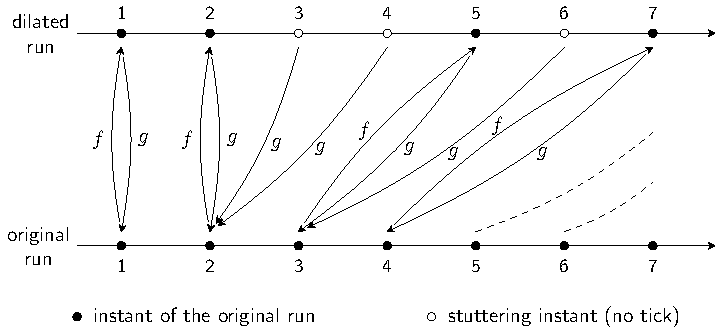
\includegraphics{dilating.pdf}
    \caption{Dilating and contracting functions}\label{fig:dilating-run}
  \end{figure}%
\end{isamarkuptext}\isamarkuptrue%
%
\begin{isamarkuptext}%
A function \isa{g} is contracting with respect to the dilation of run
\isa{sub} into run \isa{r} by the dilating function \isa{f} if:

%
\begin{itemize}%
\item it is a contracting function ;

\item \isa{{\isacharparenleft}f\ {\isasymcirc}\ g{\isacharparenright}\ n} is the index of the last original instant before instant 
\isa{n} in run \isa{r}, therefore:

%
\begin{itemize}%
\item \isa{{\isacharparenleft}f\ {\isasymcirc}\ g{\isacharparenright}\ n\ {\isasymle}\ n}

\item the time does not change on any clock between instants \isa{{\isacharparenleft}f\ {\isasymcirc}\ g{\isacharparenright}\ n}
and \isa{n} of run \isa{r};

\item no clock ticks before \isa{n} strictly after \isa{{\isacharparenleft}f\ {\isasymcirc}\ g{\isacharparenright}\ n} 
in run \isa{r}.
See \autoref{fig:dilating-run} for a better understanding. Notice that in this 
example, \isa{{\isadigit{2}}} is equal to \isa{{\isacharparenleft}f\ {\isasymcirc}\ g{\isacharparenright}\ {\isadigit{2}}}, \isa{{\isacharparenleft}f\ {\isasymcirc}\ g{\isacharparenright}\ {\isadigit{3}}}, 
and \isa{{\isacharparenleft}f\ {\isasymcirc}\ g{\isacharparenright}\ {\isadigit{4}}}. %
\end{itemize}%
\end{itemize}%
\end{isamarkuptext}\isamarkuptrue%
\isanewline
\isacommand{definition}\isamarkupfalse%
\ contracting\isanewline
\isakeyword{where}\ \isanewline
\ \ {\isacartoucheopen}contracting\ g\ r\ sub\ f\ {\isasymequiv}\ \ contracting{\isacharunderscore}fun\ g\isanewline
\ \ \ \ \ \ \ \ \ \ \ \ \ \ \ \ \ \ \ \ \ \ \ \ \ \ {\isasymand}\ {\isacharparenleft}{\isasymforall}n{\isachardot}\ f\ {\isacharparenleft}g\ n{\isacharparenright}\ {\isasymle}\ n{\isacharparenright}\isanewline
\ \ \ \ \ \ \ \ \ \ \ \ \ \ \ \ \ \ \ \ \ \ \ \ \ \ {\isasymand}\ {\isacharparenleft}{\isasymforall}n\ c\ k{\isachardot}\ f\ {\isacharparenleft}g\ n{\isacharparenright}\ {\isasymle}\ k\ {\isasymand}\ k\ {\isasymle}\ n\isanewline
\ \ \ \ \ \ \ \ \ \ \ \ \ \ \ \ \ \ \ \ \ \ \ \ \ \ \ \ \ \ {\isasymlongrightarrow}\ time\ {\isacharparenleft}{\isacharparenleft}Rep{\isacharunderscore}run\ r{\isacharparenright}\ k\ c{\isacharparenright}\ {\isacharequal}\ time\ {\isacharparenleft}{\isacharparenleft}Rep{\isacharunderscore}run\ sub{\isacharparenright}\ {\isacharparenleft}g\ n{\isacharparenright}\ c{\isacharparenright}{\isacharparenright}\isanewline
\ \ \ \ \ \ \ \ \ \ \ \ \ \ \ \ \ \ \ \ \ \ \ \ \ \ {\isasymand}\ {\isacharparenleft}{\isasymforall}n\ c\ k{\isachardot}\ f\ {\isacharparenleft}g\ n{\isacharparenright}\ {\isacharless}\ k\ {\isasymand}\ k\ {\isasymle}\ n\isanewline
\ \ \ \ \ \ \ \ \ \ \ \ \ \ \ \ \ \ \ \ \ \ \ \ \ \ \ \ \ \ {\isasymlongrightarrow}\ {\isasymnot}\ ticks\ {\isacharparenleft}{\isacharparenleft}Rep{\isacharunderscore}run\ r{\isacharparenright}\ k\ c{\isacharparenright}{\isacharparenright}{\isacartoucheclose}%
\begin{isamarkuptext}%
For any dilating function, we can build its \emph{inverse}, as illustrated on
  \autoref{fig:dilating-run}, which is a contracting function:%
\end{isamarkuptext}\isamarkuptrue%
\isacommand{definition}\isamarkupfalse%
\ {\isacartoucheopen}dil{\isacharunderscore}inverse\ f{\isacharcolon}{\isacharcolon}{\isacharparenleft}nat\ {\isasymRightarrow}\ nat{\isacharparenright}\ {\isasymequiv}\ {\isacharparenleft}{\isasymlambda}n{\isachardot}\ Max\ {\isacharbraceleft}i{\isachardot}\ f\ i\ {\isasymle}\ n{\isacharbraceright}{\isacharparenright}{\isacartoucheclose}%
\isadelimdocument
%
\endisadelimdocument
%
\isatagdocument
%
\isamarkupsubsection{Alternate definitions for counting ticks.%
}
\isamarkuptrue%
%
\endisatagdocument
{\isafolddocument}%
%
\isadelimdocument
%
\endisadelimdocument
%
\begin{isamarkuptext}%
For proving the stuttering invariance of TESL specifications, we will need
  these alternate definitions for counting ticks, which are based on sets.%
\end{isamarkuptext}\isamarkuptrue%
%
\begin{isamarkuptext}%
\isa{tick{\isacharunderscore}count\ r\ c\ n} is the number of ticks of clock \isa{c} in 
  run \isa{r} upto instant \isa{n}.%
\end{isamarkuptext}\isamarkuptrue%
\isacommand{definition}\isamarkupfalse%
\ tick{\isacharunderscore}count\ {\isacharcolon}{\isacharcolon}\ {\isacartoucheopen}{\isacharprime}a{\isacharcolon}{\isacharcolon}linordered{\isacharunderscore}field\ run\ {\isasymRightarrow}\ clock\ {\isasymRightarrow}\ nat\ {\isasymRightarrow}\ nat{\isacartoucheclose}\isanewline
\isakeyword{where}\isanewline
\ \ {\isacartoucheopen}tick{\isacharunderscore}count\ r\ c\ n\ {\isacharequal}\ card\ {\isacharbraceleft}i{\isachardot}\ i\ {\isasymle}\ n\ {\isasymand}\ ticks\ {\isacharparenleft}{\isacharparenleft}Rep{\isacharunderscore}run\ r{\isacharparenright}\ i\ c{\isacharparenright}{\isacharbraceright}{\isacartoucheclose}%
\begin{isamarkuptext}%
\isa{tick{\isacharunderscore}count{\isacharunderscore}strict\ r\ c\ n} is the number of ticks of clock \isa{c} 
  in run \isa{r} upto but excluding instant \isa{n}.%
\end{isamarkuptext}\isamarkuptrue%
\isacommand{definition}\isamarkupfalse%
\ tick{\isacharunderscore}count{\isacharunderscore}strict\ {\isacharcolon}{\isacharcolon}\ {\isacartoucheopen}{\isacharprime}a{\isacharcolon}{\isacharcolon}linordered{\isacharunderscore}field\ run\ {\isasymRightarrow}\ clock\ {\isasymRightarrow}\ nat\ {\isasymRightarrow}\ nat{\isacartoucheclose}\isanewline
\isakeyword{where}\isanewline
\ \ {\isacartoucheopen}tick{\isacharunderscore}count{\isacharunderscore}strict\ r\ c\ n\ {\isacharequal}\ card\ {\isacharbraceleft}i{\isachardot}\ i\ {\isacharless}\ n\ {\isasymand}\ ticks\ {\isacharparenleft}{\isacharparenleft}Rep{\isacharunderscore}run\ r{\isacharparenright}\ i\ c{\isacharparenright}{\isacharbraceright}{\isacartoucheclose}\isanewline
\isanewline
%
\isadelimtheory
\isanewline
%
\endisadelimtheory
%
\isatagtheory
\isacommand{end}\isamarkupfalse%
%
\endisatagtheory
{\isafoldtheory}%
%
\isadelimtheory
%
\endisadelimtheory
%
\end{isabellebody}%
\endinput
%:%file=~/Documents/Recherche/Thesards/2014_Hai_NGUYEN_VAN/Heron_git/reiher2/reiher-double-time-delayed/hygge/src/StutteringDefs.thy%:%
%:%11=1%:%
%:%15=3%:%
%:%31=5%:%
%:%32=5%:%
%:%33=6%:%
%:%34=7%:%
%:%35=8%:%
%:%36=9%:%
%:%45=12%:%
%:%46=13%:%
%:%47=14%:%
%:%48=15%:%
%:%49=16%:%
%:%58=19%:%
%:%70=22%:%
%:%71=23%:%
%:%72=24%:%
%:%73=25%:%
%:%74=26%:%
%:%78=27%:%
%:%80=28%:%
%:%81=29%:%
%:%83=30%:%
%:%84=31%:%
%:%86=32%:%
%:%87=33%:%
%:%90=35%:%
%:%91=35%:%
%:%92=36%:%
%:%93=37%:%
%:%100=45%:%
%:%101=46%:%
%:%105=47%:%
%:%107=48%:%
%:%109=49%:%
%:%112=51%:%
%:%113=51%:%
%:%114=52%:%
%:%115=53%:%
%:%119=58%:%
%:%121=60%:%
%:%122=60%:%
%:%123=61%:%
%:%124=62%:%
%:%126=65%:%
%:%127=66%:%
%:%128=67%:%
%:%129=68%:%
%:%130=69%:%
%:%131=70%:%
%:%132=71%:%
%:%134=73%:%
%:%135=73%:%
%:%136=74%:%
%:%138=77%:%
%:%139=78%:%
%:%140=79%:%
%:%141=80%:%
%:%142=81%:%
%:%143=82%:%
%:%144=83%:%
%:%145=84%:%
%:%149=96%:%
%:%150=97%:%
%:%154=98%:%
%:%156=99%:%
%:%157=100%:%
%:%163=102%:%
%:%164=103%:%
%:%166=104%:%
%:%167=105%:%
%:%168=106%:%
%:%169=107%:%
%:%170=108%:%
%:%174=115%:%
%:%175=116%:%
%:%176=116%:%
%:%177=117%:%
%:%178=118%:%
%:%185=126%:%
%:%186=127%:%
%:%188=129%:%
%:%189=129%:%
%:%196=132%:%
%:%208=135%:%
%:%209=136%:%
%:%213=140%:%
%:%214=141%:%
%:%216=143%:%
%:%217=143%:%
%:%218=144%:%
%:%219=145%:%
%:%221=148%:%
%:%222=149%:%
%:%224=151%:%
%:%225=151%:%
%:%226=152%:%
%:%227=153%:%
%:%228=154%:%
%:%231=155%:%
%:%236=156%:%

%
\begin{isabellebody}%
\setisabellecontext{StutteringLemmas}%
%
\isadelimdocument
%
\endisadelimdocument
%
\isatagdocument
%
\isamarkupsubsection{Stuttering Lemmas%
}
\isamarkuptrue%
%
\endisatagdocument
{\isafolddocument}%
%
\isadelimdocument
%
\endisadelimdocument
%
\isadelimtheory
%
\endisadelimtheory
%
\isatagtheory
\isacommand{theory}\isamarkupfalse%
\ StutteringLemmas\isanewline
\isanewline
\isakeyword{imports}\ StutteringDefs\isanewline
\isanewline
\isakeyword{begin}%
\endisatagtheory
{\isafoldtheory}%
%
\isadelimtheory
\isanewline
%
\endisadelimtheory
\isanewline
\isacommand{lemma}\isamarkupfalse%
\ bounded{\isacharunderscore}suc{\isacharunderscore}ind{\isacharcolon}\isanewline
\ \ \isakeyword{assumes}\ {\isacartoucheopen}{\isasymAnd}k{\isachardot}\ k\ {\isacharless}\ m\ {\isasymLongrightarrow}\ P\ {\isacharparenleft}Suc\ {\isacharparenleft}z\ {\isacharplus}\ k{\isacharparenright}{\isacharparenright}\ {\isacharequal}\ P\ {\isacharparenleft}z\ {\isacharplus}\ k{\isacharparenright}{\isacartoucheclose}\isanewline
\ \ \ \ \isakeyword{shows}\ {\isacartoucheopen}k\ {\isacharless}\ m\ {\isasymLongrightarrow}\ P\ {\isacharparenleft}Suc\ {\isacharparenleft}z\ {\isacharplus}\ k{\isacharparenright}{\isacharparenright}\ {\isacharequal}\ P\ z{\isacartoucheclose}\isanewline
%
\isadelimproof
%
\endisadelimproof
%
\isatagproof
\isacommand{proof}\isamarkupfalse%
\ {\isacharparenleft}induction\ k{\isacharparenright}\isanewline
\ \ \isacommand{case}\isamarkupfalse%
\ {\isadigit{0}}\isanewline
\ \ \ \ \isacommand{with}\isamarkupfalse%
\ assms{\isacharparenleft}{\isadigit{1}}{\isacharparenright}{\isacharbrackleft}of\ {\isadigit{0}}{\isacharbrackright}\ \isacommand{show}\isamarkupfalse%
\ {\isacharquery}case\ \isacommand{by}\isamarkupfalse%
\ simp\isanewline
\isacommand{next}\isamarkupfalse%
\isanewline
\ \ \isacommand{case}\isamarkupfalse%
\ {\isacharparenleft}Suc\ k{\isacharprime}{\isacharparenright}\isanewline
\ \ \ \ \isacommand{with}\isamarkupfalse%
\ assms{\isacharbrackleft}of\ {\isacartoucheopen}Suc\ k{\isacharprime}{\isacartoucheclose}{\isacharbrackright}\ \isacommand{show}\isamarkupfalse%
\ {\isacharquery}case\ \isacommand{by}\isamarkupfalse%
\ force\isanewline
\isacommand{qed}\isamarkupfalse%
%
\endisatagproof
{\isafoldproof}%
%
\isadelimproof
%
\endisadelimproof
%
\isadelimdocument
%
\endisadelimdocument
%
\isatagdocument
%
\isamarkupsubsection{Lemmas used to prove the invariance by stuttering%
}
\isamarkuptrue%
%
\endisatagdocument
{\isafolddocument}%
%
\isadelimdocument
%
\endisadelimdocument
%
\begin{isamarkuptext}%
A dilating function is injective.%
\end{isamarkuptext}\isamarkuptrue%
\isacommand{lemma}\isamarkupfalse%
\ dilating{\isacharunderscore}fun{\isacharunderscore}injects{\isacharcolon}\isanewline
\ \ \isakeyword{assumes}\ {\isacartoucheopen}dilating{\isacharunderscore}fun\ f\ r{\isacartoucheclose}\isanewline
\ \ \isakeyword{shows}\ \ \ {\isacartoucheopen}inj{\isacharunderscore}on\ f\ A{\isacartoucheclose}\isanewline
%
\isadelimproof
%
\endisadelimproof
%
\isatagproof
\isacommand{using}\isamarkupfalse%
\ assms\ dilating{\isacharunderscore}fun{\isacharunderscore}def\ strict{\isacharunderscore}mono{\isacharunderscore}imp{\isacharunderscore}inj{\isacharunderscore}on\ \isacommand{by}\isamarkupfalse%
\ blast%
\endisatagproof
{\isafoldproof}%
%
\isadelimproof
%
\endisadelimproof
%
\begin{isamarkuptext}%
If a clock ticks at an instant in a dilated run, that instant is the image
  by the dilating function of an instant of the original run.%
\end{isamarkuptext}\isamarkuptrue%
\isacommand{lemma}\isamarkupfalse%
\ ticks{\isacharunderscore}image{\isacharcolon}\isanewline
\ \ \isakeyword{assumes}\ {\isacartoucheopen}dilating{\isacharunderscore}fun\ f\ r{\isacartoucheclose}\isanewline
\ \ \isakeyword{and}\ \ \ \ \ {\isacartoucheopen}hamlet\ {\isacharparenleft}{\isacharparenleft}Rep{\isacharunderscore}run\ r{\isacharparenright}\ n\ c{\isacharparenright}{\isacartoucheclose}\isanewline
\ \ \isakeyword{shows}\ \ \ {\isacartoucheopen}{\isasymexists}n\isactrlsub {\isadigit{0}}{\isachardot}\ f\ n\isactrlsub {\isadigit{0}}\ {\isacharequal}\ n{\isacartoucheclose}\isanewline
%
\isadelimproof
%
\endisadelimproof
%
\isatagproof
\isacommand{using}\isamarkupfalse%
\ dilating{\isacharunderscore}fun{\isacharunderscore}def\ assms\ \isacommand{by}\isamarkupfalse%
\ blast%
\endisatagproof
{\isafoldproof}%
%
\isadelimproof
%
\endisadelimproof
%
\begin{isamarkuptext}%
The image of the ticks in a interval by a dilating function is the interval 
  bounded by the image of the bound of the original interval.
  This is proven for all 4 kinds of intervals:  \isatt{]m{\char`\,}\ n[}, \isatt{[m{\char`\,}\ n[}, \isatt{]m{\char`\,}\ n]} and \isatt{[m{\char`\,}\ n]}.%
\end{isamarkuptext}\isamarkuptrue%
\isacommand{lemma}\isamarkupfalse%
\ dilating{\isacharunderscore}fun{\isacharunderscore}image{\isacharunderscore}strict{\isacharcolon}\isanewline
\ \ \isakeyword{assumes}\ {\isacartoucheopen}dilating{\isacharunderscore}fun\ f\ r{\isacartoucheclose}\isanewline
\ \ \isakeyword{shows}\ \ \ {\isacartoucheopen}{\isacharbraceleft}k{\isachardot}\ f\ m\ {\isacharless}\ k\ {\isasymand}\ k\ {\isacharless}\ f\ n\ {\isasymand}\ hamlet\ {\isacharparenleft}{\isacharparenleft}Rep{\isacharunderscore}run\ r{\isacharparenright}\ k\ c{\isacharparenright}{\isacharbraceright}\isanewline
\ \ \ \ \ \ \ \ \ \ \ \ {\isacharequal}\ image\ f\ {\isacharbraceleft}k{\isachardot}\ m\ {\isacharless}\ k\ {\isasymand}\ k\ {\isacharless}\ n\ {\isasymand}\ hamlet\ {\isacharparenleft}{\isacharparenleft}Rep{\isacharunderscore}run\ r{\isacharparenright}\ {\isacharparenleft}f\ k{\isacharparenright}\ c{\isacharparenright}{\isacharbraceright}{\isacartoucheclose}\isanewline
\ \ {\isacharparenleft}\isakeyword{is}\ {\isacartoucheopen}{\isacharquery}IMG\ {\isacharequal}\ image\ f\ {\isacharquery}SET{\isacartoucheclose}{\isacharparenright}\isanewline
%
\isadelimproof
%
\endisadelimproof
%
\isatagproof
\isacommand{proof}\isamarkupfalse%
\isanewline
\ \ \isacommand{{\isacharbraceleft}}\isamarkupfalse%
\ \isacommand{fix}\isamarkupfalse%
\ k\ \isacommand{assume}\isamarkupfalse%
\ h{\isacharcolon}{\isacartoucheopen}k\ {\isasymin}\ {\isacharquery}IMG{\isacartoucheclose}\isanewline
\ \ \ \ \isacommand{from}\isamarkupfalse%
\ h\ \isacommand{obtain}\isamarkupfalse%
\ k\isactrlsub {\isadigit{0}}\ \isakeyword{where}\ k{\isadigit{0}}prop{\isacharcolon}{\isacartoucheopen}f\ k\isactrlsub {\isadigit{0}}\ {\isacharequal}\ k\ {\isasymand}\ hamlet\ {\isacharparenleft}{\isacharparenleft}Rep{\isacharunderscore}run\ r{\isacharparenright}\ {\isacharparenleft}f\ k\isactrlsub {\isadigit{0}}{\isacharparenright}\ c{\isacharparenright}{\isacartoucheclose}\isanewline
\ \ \ \ \ \ \isacommand{using}\isamarkupfalse%
\ ticks{\isacharunderscore}image{\isacharbrackleft}OF\ assms{\isacharbrackright}\ \isacommand{by}\isamarkupfalse%
\ blast\isanewline
\ \ \ \ \isacommand{with}\isamarkupfalse%
\ h\ \isacommand{have}\isamarkupfalse%
\ {\isacartoucheopen}k\ {\isasymin}\ image\ f\ {\isacharquery}SET{\isacartoucheclose}\ \isacommand{using}\isamarkupfalse%
\ assms\ dilating{\isacharunderscore}fun{\isacharunderscore}def\ strict{\isacharunderscore}mono{\isacharunderscore}less\ \isacommand{by}\isamarkupfalse%
\ blast\isanewline
\ \ \isacommand{{\isacharbraceright}}\isamarkupfalse%
\ \isacommand{thus}\isamarkupfalse%
\ {\isacartoucheopen}{\isacharquery}IMG\ {\isasymsubseteq}\ image\ f\ {\isacharquery}SET{\isacartoucheclose}\ \isacommand{{\isachardot}{\isachardot}}\isamarkupfalse%
\isanewline
\isacommand{next}\isamarkupfalse%
\isanewline
\ \ \isacommand{{\isacharbraceleft}}\isamarkupfalse%
\ \isacommand{fix}\isamarkupfalse%
\ k\ \isacommand{assume}\isamarkupfalse%
\ h{\isacharcolon}{\isacartoucheopen}k\ {\isasymin}\ image\ f\ {\isacharquery}SET{\isacartoucheclose}\isanewline
\ \ \ \ \isacommand{from}\isamarkupfalse%
\ h\ \isacommand{obtain}\isamarkupfalse%
\ k\isactrlsub {\isadigit{0}}\ \isakeyword{where}\ k{\isadigit{0}}prop{\isacharcolon}{\isacartoucheopen}k\ {\isacharequal}\ f\ k\isactrlsub {\isadigit{0}}\ {\isasymand}\ k\isactrlsub {\isadigit{0}}\ {\isasymin}\ {\isacharquery}SET{\isacartoucheclose}\ \isacommand{by}\isamarkupfalse%
\ blast\isanewline
\ \ \ \ \isacommand{hence}\isamarkupfalse%
\ {\isacartoucheopen}k\ {\isasymin}\ {\isacharquery}IMG{\isacartoucheclose}\ \isacommand{using}\isamarkupfalse%
\ assms\ \isacommand{by}\isamarkupfalse%
\ {\isacharparenleft}simp\ add{\isacharcolon}\ dilating{\isacharunderscore}fun{\isacharunderscore}def\ strict{\isacharunderscore}mono{\isacharunderscore}less{\isacharparenright}\isanewline
\ \ \isacommand{{\isacharbraceright}}\isamarkupfalse%
\ \isacommand{thus}\isamarkupfalse%
\ {\isacartoucheopen}image\ f\ {\isacharquery}SET\ {\isasymsubseteq}\ {\isacharquery}IMG{\isacartoucheclose}\ \isacommand{{\isachardot}{\isachardot}}\isamarkupfalse%
\isanewline
\isacommand{qed}\isamarkupfalse%
%
\endisatagproof
{\isafoldproof}%
%
\isadelimproof
\isanewline
%
\endisadelimproof
\isanewline
\isacommand{lemma}\isamarkupfalse%
\ dilating{\isacharunderscore}fun{\isacharunderscore}image{\isacharunderscore}left{\isacharcolon}\isanewline
\ \ \isakeyword{assumes}\ {\isacartoucheopen}dilating{\isacharunderscore}fun\ f\ r{\isacartoucheclose}\isanewline
\ \ \isakeyword{shows}\ \ \ {\isacartoucheopen}{\isacharbraceleft}k{\isachardot}\ f\ m\ {\isasymle}\ k\ {\isasymand}\ k\ {\isacharless}\ f\ n\ {\isasymand}\ hamlet\ {\isacharparenleft}{\isacharparenleft}Rep{\isacharunderscore}run\ r{\isacharparenright}\ k\ c{\isacharparenright}{\isacharbraceright}\isanewline
\ \ \ \ \ \ \ \ \ \ {\isacharequal}\ image\ f\ {\isacharbraceleft}k{\isachardot}\ m\ {\isasymle}\ k\ {\isasymand}\ k\ {\isacharless}\ n\ {\isasymand}\ hamlet\ {\isacharparenleft}{\isacharparenleft}Rep{\isacharunderscore}run\ r{\isacharparenright}\ {\isacharparenleft}f\ k{\isacharparenright}\ c{\isacharparenright}{\isacharbraceright}{\isacartoucheclose}\isanewline
\ \ {\isacharparenleft}\isakeyword{is}\ {\isacartoucheopen}{\isacharquery}IMG\ {\isacharequal}\ image\ f\ {\isacharquery}SET{\isacartoucheclose}{\isacharparenright}\isanewline
%
\isadelimproof
%
\endisadelimproof
%
\isatagproof
\isacommand{proof}\isamarkupfalse%
\isanewline
\ \ \isacommand{{\isacharbraceleft}}\isamarkupfalse%
\ \isacommand{fix}\isamarkupfalse%
\ k\ \isacommand{assume}\isamarkupfalse%
\ h{\isacharcolon}{\isacartoucheopen}k\ {\isasymin}\ {\isacharquery}IMG{\isacartoucheclose}\isanewline
\ \ \ \ \isacommand{from}\isamarkupfalse%
\ h\ \isacommand{obtain}\isamarkupfalse%
\ k\isactrlsub {\isadigit{0}}\ \isakeyword{where}\ k{\isadigit{0}}prop{\isacharcolon}{\isacartoucheopen}f\ k\isactrlsub {\isadigit{0}}\ {\isacharequal}\ k\ {\isasymand}\ hamlet\ {\isacharparenleft}{\isacharparenleft}Rep{\isacharunderscore}run\ r{\isacharparenright}\ {\isacharparenleft}f\ k\isactrlsub {\isadigit{0}}{\isacharparenright}\ c{\isacharparenright}{\isacartoucheclose}\isanewline
\ \ \ \ \ \ \isacommand{using}\isamarkupfalse%
\ ticks{\isacharunderscore}image{\isacharbrackleft}OF\ assms{\isacharbrackright}\ \isacommand{by}\isamarkupfalse%
\ blast\isanewline
\ \ \ \ \isacommand{with}\isamarkupfalse%
\ h\ \isacommand{have}\isamarkupfalse%
\ {\isacartoucheopen}k\ {\isasymin}\ image\ f\ {\isacharquery}SET{\isacartoucheclose}\isanewline
\ \ \ \ \ \ \isacommand{using}\isamarkupfalse%
\ assms\ dilating{\isacharunderscore}fun{\isacharunderscore}def\ strict{\isacharunderscore}mono{\isacharunderscore}less\ strict{\isacharunderscore}mono{\isacharunderscore}less{\isacharunderscore}eq\ \isacommand{by}\isamarkupfalse%
\ fastforce\isanewline
\ \ \isacommand{{\isacharbraceright}}\isamarkupfalse%
\ \isacommand{thus}\isamarkupfalse%
\ {\isacartoucheopen}{\isacharquery}IMG\ {\isasymsubseteq}\ image\ f\ {\isacharquery}SET{\isacartoucheclose}\ \isacommand{{\isachardot}{\isachardot}}\isamarkupfalse%
\isanewline
\isacommand{next}\isamarkupfalse%
\isanewline
\ \ \isacommand{{\isacharbraceleft}}\isamarkupfalse%
\ \isacommand{fix}\isamarkupfalse%
\ k\ \isacommand{assume}\isamarkupfalse%
\ h{\isacharcolon}{\isacartoucheopen}k\ {\isasymin}\ image\ f\ {\isacharquery}SET{\isacartoucheclose}\isanewline
\ \ \ \ \isacommand{from}\isamarkupfalse%
\ h\ \isacommand{obtain}\isamarkupfalse%
\ k\isactrlsub {\isadigit{0}}\ \isakeyword{where}\ k{\isadigit{0}}prop{\isacharcolon}{\isacartoucheopen}k\ {\isacharequal}\ f\ k\isactrlsub {\isadigit{0}}\ {\isasymand}\ k\isactrlsub {\isadigit{0}}\ {\isasymin}\ {\isacharquery}SET{\isacartoucheclose}\ \isacommand{by}\isamarkupfalse%
\ blast\isanewline
\ \ \ \ \isacommand{hence}\isamarkupfalse%
\ {\isacartoucheopen}k\ {\isasymin}\ {\isacharquery}IMG{\isacartoucheclose}\isanewline
\ \ \ \ \ \ \isacommand{using}\isamarkupfalse%
\ assms\ dilating{\isacharunderscore}fun{\isacharunderscore}def\ strict{\isacharunderscore}mono{\isacharunderscore}less\ strict{\isacharunderscore}mono{\isacharunderscore}less{\isacharunderscore}eq\ \isacommand{by}\isamarkupfalse%
\ fastforce\isanewline
\ \ \isacommand{{\isacharbraceright}}\isamarkupfalse%
\ \isacommand{thus}\isamarkupfalse%
\ {\isacartoucheopen}image\ f\ {\isacharquery}SET\ {\isasymsubseteq}\ {\isacharquery}IMG{\isacartoucheclose}\ \isacommand{{\isachardot}{\isachardot}}\isamarkupfalse%
\isanewline
\isacommand{qed}\isamarkupfalse%
%
\endisatagproof
{\isafoldproof}%
%
\isadelimproof
\isanewline
%
\endisadelimproof
\isanewline
\isacommand{lemma}\isamarkupfalse%
\ dilating{\isacharunderscore}fun{\isacharunderscore}image{\isacharunderscore}right{\isacharcolon}\isanewline
\ \ \isakeyword{assumes}\ {\isacartoucheopen}dilating{\isacharunderscore}fun\ f\ r{\isacartoucheclose}\isanewline
\ \ \isakeyword{shows}\ \ \ {\isacartoucheopen}{\isacharbraceleft}k{\isachardot}\ f\ m\ {\isacharless}\ k\ {\isasymand}\ k\ {\isasymle}\ f\ n\ {\isasymand}\ hamlet\ {\isacharparenleft}{\isacharparenleft}Rep{\isacharunderscore}run\ r{\isacharparenright}\ k\ c{\isacharparenright}{\isacharbraceright}\isanewline
\ \ \ \ \ \ \ \ \ \ {\isacharequal}\ image\ f\ {\isacharbraceleft}k{\isachardot}\ m\ {\isacharless}\ k\ {\isasymand}\ k\ {\isasymle}\ n\ {\isasymand}\ hamlet\ {\isacharparenleft}{\isacharparenleft}Rep{\isacharunderscore}run\ r{\isacharparenright}\ {\isacharparenleft}f\ k{\isacharparenright}\ c{\isacharparenright}{\isacharbraceright}{\isacartoucheclose}\isanewline
\ \ {\isacharparenleft}\isakeyword{is}\ {\isacartoucheopen}{\isacharquery}IMG\ {\isacharequal}\ image\ f\ {\isacharquery}SET{\isacartoucheclose}{\isacharparenright}\isanewline
%
\isadelimproof
%
\endisadelimproof
%
\isatagproof
\isacommand{proof}\isamarkupfalse%
\isanewline
\ \ \isacommand{{\isacharbraceleft}}\isamarkupfalse%
\ \isacommand{fix}\isamarkupfalse%
\ k\ \isacommand{assume}\isamarkupfalse%
\ h{\isacharcolon}{\isacartoucheopen}k\ {\isasymin}\ {\isacharquery}IMG{\isacartoucheclose}\isanewline
\ \ \ \ \isacommand{from}\isamarkupfalse%
\ h\ \isacommand{obtain}\isamarkupfalse%
\ k\isactrlsub {\isadigit{0}}\ \isakeyword{where}\ k{\isadigit{0}}prop{\isacharcolon}{\isacartoucheopen}f\ k\isactrlsub {\isadigit{0}}\ {\isacharequal}\ k\ {\isasymand}\ hamlet\ {\isacharparenleft}{\isacharparenleft}Rep{\isacharunderscore}run\ r{\isacharparenright}\ {\isacharparenleft}f\ k\isactrlsub {\isadigit{0}}{\isacharparenright}\ c{\isacharparenright}{\isacartoucheclose}\isanewline
\ \ \ \ \ \ \isacommand{using}\isamarkupfalse%
\ ticks{\isacharunderscore}image{\isacharbrackleft}OF\ assms{\isacharbrackright}\ \isacommand{by}\isamarkupfalse%
\ blast\isanewline
\ \ \ \ \isacommand{with}\isamarkupfalse%
\ h\ \isacommand{have}\isamarkupfalse%
\ {\isacartoucheopen}k\ {\isasymin}\ image\ f\ {\isacharquery}SET{\isacartoucheclose}\isanewline
\ \ \ \ \ \ \isacommand{using}\isamarkupfalse%
\ assms\ dilating{\isacharunderscore}fun{\isacharunderscore}def\ strict{\isacharunderscore}mono{\isacharunderscore}less\ strict{\isacharunderscore}mono{\isacharunderscore}less{\isacharunderscore}eq\ \isacommand{by}\isamarkupfalse%
\ fastforce\isanewline
\ \ \isacommand{{\isacharbraceright}}\isamarkupfalse%
\ \isacommand{thus}\isamarkupfalse%
\ {\isacartoucheopen}{\isacharquery}IMG\ {\isasymsubseteq}\ image\ f\ {\isacharquery}SET{\isacartoucheclose}\ \isacommand{{\isachardot}{\isachardot}}\isamarkupfalse%
\isanewline
\isacommand{next}\isamarkupfalse%
\isanewline
\ \ \isacommand{{\isacharbraceleft}}\isamarkupfalse%
\ \isacommand{fix}\isamarkupfalse%
\ k\ \isacommand{assume}\isamarkupfalse%
\ h{\isacharcolon}{\isacartoucheopen}k\ {\isasymin}\ image\ f\ {\isacharquery}SET{\isacartoucheclose}\isanewline
\ \ \ \ \isacommand{from}\isamarkupfalse%
\ h\ \isacommand{obtain}\isamarkupfalse%
\ k\isactrlsub {\isadigit{0}}\ \isakeyword{where}\ k{\isadigit{0}}prop{\isacharcolon}{\isacartoucheopen}k\ {\isacharequal}\ f\ k\isactrlsub {\isadigit{0}}\ {\isasymand}\ k\isactrlsub {\isadigit{0}}\ {\isasymin}\ {\isacharquery}SET{\isacartoucheclose}\ \isacommand{by}\isamarkupfalse%
\ blast\isanewline
\ \ \ \ \isacommand{hence}\isamarkupfalse%
\ {\isacartoucheopen}k\ {\isasymin}\ {\isacharquery}IMG{\isacartoucheclose}\isanewline
\ \ \ \ \ \ \isacommand{using}\isamarkupfalse%
\ assms\ dilating{\isacharunderscore}fun{\isacharunderscore}def\ strict{\isacharunderscore}mono{\isacharunderscore}less\ strict{\isacharunderscore}mono{\isacharunderscore}less{\isacharunderscore}eq\ \isacommand{by}\isamarkupfalse%
\ fastforce\isanewline
\ \ \isacommand{{\isacharbraceright}}\isamarkupfalse%
\ \isacommand{thus}\isamarkupfalse%
\ {\isacartoucheopen}image\ f\ {\isacharquery}SET\ {\isasymsubseteq}\ {\isacharquery}IMG{\isacartoucheclose}\ \isacommand{{\isachardot}{\isachardot}}\isamarkupfalse%
\isanewline
\isacommand{qed}\isamarkupfalse%
%
\endisatagproof
{\isafoldproof}%
%
\isadelimproof
\isanewline
%
\endisadelimproof
\isanewline
\isacommand{lemma}\isamarkupfalse%
\ dilating{\isacharunderscore}fun{\isacharunderscore}image{\isacharcolon}\isanewline
\ \ \isakeyword{assumes}\ {\isacartoucheopen}dilating{\isacharunderscore}fun\ f\ r{\isacartoucheclose}\isanewline
\ \ \isakeyword{shows}\ \ \ {\isacartoucheopen}{\isacharbraceleft}k{\isachardot}\ f\ m\ {\isasymle}\ k\ {\isasymand}\ k\ {\isasymle}\ f\ n\ {\isasymand}\ hamlet\ {\isacharparenleft}{\isacharparenleft}Rep{\isacharunderscore}run\ r{\isacharparenright}\ k\ c{\isacharparenright}{\isacharbraceright}\isanewline
\ \ \ \ \ \ \ \ \ \ {\isacharequal}\ image\ f\ {\isacharbraceleft}k{\isachardot}\ m\ {\isasymle}\ k\ {\isasymand}\ k\ {\isasymle}\ n\ {\isasymand}\ hamlet\ {\isacharparenleft}{\isacharparenleft}Rep{\isacharunderscore}run\ r{\isacharparenright}\ {\isacharparenleft}f\ k{\isacharparenright}\ c{\isacharparenright}{\isacharbraceright}{\isacartoucheclose}\isanewline
\ \ {\isacharparenleft}\isakeyword{is}\ {\isacartoucheopen}{\isacharquery}IMG\ {\isacharequal}\ image\ f\ {\isacharquery}SET{\isacartoucheclose}{\isacharparenright}\isanewline
%
\isadelimproof
%
\endisadelimproof
%
\isatagproof
\isacommand{proof}\isamarkupfalse%
\isanewline
\ \ \isacommand{{\isacharbraceleft}}\isamarkupfalse%
\ \isacommand{fix}\isamarkupfalse%
\ k\ \isacommand{assume}\isamarkupfalse%
\ h{\isacharcolon}{\isacartoucheopen}k\ {\isasymin}\ {\isacharquery}IMG{\isacartoucheclose}\isanewline
\ \ \ \ \isacommand{from}\isamarkupfalse%
\ h\ \isacommand{obtain}\isamarkupfalse%
\ k\isactrlsub {\isadigit{0}}\ \isakeyword{where}\ k{\isadigit{0}}prop{\isacharcolon}{\isacartoucheopen}f\ k\isactrlsub {\isadigit{0}}\ {\isacharequal}\ k\ {\isasymand}\ hamlet\ {\isacharparenleft}{\isacharparenleft}Rep{\isacharunderscore}run\ r{\isacharparenright}\ {\isacharparenleft}f\ k\isactrlsub {\isadigit{0}}{\isacharparenright}\ c{\isacharparenright}{\isacartoucheclose}\isanewline
\ \ \ \ \ \ \isacommand{using}\isamarkupfalse%
\ ticks{\isacharunderscore}image{\isacharbrackleft}OF\ assms{\isacharbrackright}\ \isacommand{by}\isamarkupfalse%
\ blast\isanewline
\ \ \ \ \isacommand{with}\isamarkupfalse%
\ h\ \isacommand{have}\isamarkupfalse%
\ {\isacartoucheopen}k\ {\isasymin}\ image\ f\ {\isacharquery}SET{\isacartoucheclose}\isanewline
\ \ \ \ \ \ \isacommand{using}\isamarkupfalse%
\ assms\ dilating{\isacharunderscore}fun{\isacharunderscore}def\ strict{\isacharunderscore}mono{\isacharunderscore}less{\isacharunderscore}eq\ \isacommand{by}\isamarkupfalse%
\ blast\isanewline
\ \ \isacommand{{\isacharbraceright}}\isamarkupfalse%
\ \isacommand{thus}\isamarkupfalse%
\ {\isacartoucheopen}{\isacharquery}IMG\ {\isasymsubseteq}\ image\ f\ {\isacharquery}SET{\isacartoucheclose}\ \isacommand{{\isachardot}{\isachardot}}\isamarkupfalse%
\isanewline
\isacommand{next}\isamarkupfalse%
\isanewline
\ \ \isacommand{{\isacharbraceleft}}\isamarkupfalse%
\ \isacommand{fix}\isamarkupfalse%
\ k\ \isacommand{assume}\isamarkupfalse%
\ h{\isacharcolon}{\isacartoucheopen}k\ {\isasymin}\ image\ f\ {\isacharquery}SET{\isacartoucheclose}\isanewline
\ \ \ \ \isacommand{from}\isamarkupfalse%
\ h\ \isacommand{obtain}\isamarkupfalse%
\ k\isactrlsub {\isadigit{0}}\ \isakeyword{where}\ k{\isadigit{0}}prop{\isacharcolon}{\isacartoucheopen}k\ {\isacharequal}\ f\ k\isactrlsub {\isadigit{0}}\ {\isasymand}\ k\isactrlsub {\isadigit{0}}\ {\isasymin}\ {\isacharquery}SET{\isacartoucheclose}\ \isacommand{by}\isamarkupfalse%
\ blast\isanewline
\ \ \ \ \isacommand{hence}\isamarkupfalse%
\ {\isacartoucheopen}k\ {\isasymin}\ {\isacharquery}IMG{\isacartoucheclose}\ \isacommand{using}\isamarkupfalse%
\ assms\ \isacommand{by}\isamarkupfalse%
\ {\isacharparenleft}simp\ add{\isacharcolon}\ dilating{\isacharunderscore}fun{\isacharunderscore}def\ strict{\isacharunderscore}mono{\isacharunderscore}less{\isacharunderscore}eq{\isacharparenright}\isanewline
\ \ \isacommand{{\isacharbraceright}}\isamarkupfalse%
\ \isacommand{thus}\isamarkupfalse%
\ {\isacartoucheopen}image\ f\ {\isacharquery}SET\ {\isasymsubseteq}\ {\isacharquery}IMG{\isacartoucheclose}\ \isacommand{{\isachardot}{\isachardot}}\isamarkupfalse%
\isanewline
\isacommand{qed}\isamarkupfalse%
%
\endisatagproof
{\isafoldproof}%
%
\isadelimproof
%
\endisadelimproof
%
\begin{isamarkuptext}%
On any clock, the number of ticks in an interval is preserved
  by a dilating function.%
\end{isamarkuptext}\isamarkuptrue%
\isacommand{lemma}\isamarkupfalse%
\ ticks{\isacharunderscore}as{\isacharunderscore}often{\isacharunderscore}strict{\isacharcolon}\isanewline
\ \ \isakeyword{assumes}\ {\isacartoucheopen}dilating{\isacharunderscore}fun\ f\ r{\isacartoucheclose}\isanewline
\ \ \isakeyword{shows}\ \ \ {\isacartoucheopen}card\ {\isacharbraceleft}p{\isachardot}\ n\ {\isacharless}\ p\ {\isasymand}\ p\ {\isacharless}\ m\ {\isasymand}\ hamlet\ {\isacharparenleft}{\isacharparenleft}Rep{\isacharunderscore}run\ r{\isacharparenright}\ {\isacharparenleft}f\ p{\isacharparenright}\ c{\isacharparenright}{\isacharbraceright}\isanewline
\ \ \ \ \ \ \ \ \ \ {\isacharequal}\ card\ {\isacharbraceleft}p{\isachardot}\ f\ n\ {\isacharless}\ p\ {\isasymand}\ p\ {\isacharless}\ f\ m\ {\isasymand}\ hamlet\ {\isacharparenleft}{\isacharparenleft}Rep{\isacharunderscore}run\ r{\isacharparenright}\ p\ c{\isacharparenright}{\isacharbraceright}{\isacartoucheclose}\isanewline
\ \ \ \ {\isacharparenleft}\isakeyword{is}\ {\isacartoucheopen}card\ {\isacharquery}SET\ {\isacharequal}\ card\ {\isacharquery}IMG{\isacartoucheclose}{\isacharparenright}\isanewline
%
\isadelimproof
%
\endisadelimproof
%
\isatagproof
\isacommand{proof}\isamarkupfalse%
\ {\isacharminus}\isanewline
\ \ \isacommand{from}\isamarkupfalse%
\ dilating{\isacharunderscore}fun{\isacharunderscore}injects{\isacharbrackleft}OF\ assms{\isacharbrackright}\ \isacommand{have}\isamarkupfalse%
\ {\isacartoucheopen}inj{\isacharunderscore}on\ f\ {\isacharquery}SET{\isacartoucheclose}\ \isacommand{{\isachardot}}\isamarkupfalse%
\isanewline
\ \ \isacommand{moreover}\isamarkupfalse%
\ \isacommand{have}\isamarkupfalse%
\ {\isacartoucheopen}finite\ {\isacharquery}SET{\isacartoucheclose}\ \isacommand{by}\isamarkupfalse%
\ simp\isanewline
\ \ \isacommand{from}\isamarkupfalse%
\ inj{\isacharunderscore}on{\isacharunderscore}iff{\isacharunderscore}eq{\isacharunderscore}card{\isacharbrackleft}OF\ this{\isacharbrackright}\ calculation\ \isacommand{have}\isamarkupfalse%
\ {\isacartoucheopen}card\ {\isacharparenleft}image\ f\ {\isacharquery}SET{\isacharparenright}\ {\isacharequal}\ card\ {\isacharquery}SET{\isacartoucheclose}\ \isacommand{by}\isamarkupfalse%
\ blast\isanewline
\ \ \isacommand{moreover}\isamarkupfalse%
\ \isacommand{from}\isamarkupfalse%
\ dilating{\isacharunderscore}fun{\isacharunderscore}image{\isacharunderscore}strict{\isacharbrackleft}OF\ assms{\isacharbrackright}\ \isacommand{have}\isamarkupfalse%
\ {\isacartoucheopen}{\isacharquery}IMG\ {\isacharequal}\ image\ f\ {\isacharquery}SET{\isacartoucheclose}\ \isacommand{{\isachardot}}\isamarkupfalse%
\isanewline
\ \ \isacommand{ultimately}\isamarkupfalse%
\ \isacommand{show}\isamarkupfalse%
\ {\isacharquery}thesis\ \isacommand{by}\isamarkupfalse%
\ auto\isanewline
\isacommand{qed}\isamarkupfalse%
%
\endisatagproof
{\isafoldproof}%
%
\isadelimproof
\isanewline
%
\endisadelimproof
\isanewline
\isacommand{lemma}\isamarkupfalse%
\ ticks{\isacharunderscore}as{\isacharunderscore}often{\isacharunderscore}left{\isacharcolon}\isanewline
\ \ \isakeyword{assumes}\ {\isacartoucheopen}dilating{\isacharunderscore}fun\ f\ r{\isacartoucheclose}\isanewline
\ \ \isakeyword{shows}\ \ \ {\isacartoucheopen}card\ {\isacharbraceleft}p{\isachardot}\ n\ {\isasymle}\ p\ {\isasymand}\ p\ {\isacharless}\ m\ {\isasymand}\ hamlet\ {\isacharparenleft}{\isacharparenleft}Rep{\isacharunderscore}run\ r{\isacharparenright}\ {\isacharparenleft}f\ p{\isacharparenright}\ c{\isacharparenright}{\isacharbraceright}\isanewline
\ \ \ \ \ \ \ \ \ \ {\isacharequal}\ card\ {\isacharbraceleft}p{\isachardot}\ f\ n\ {\isasymle}\ p\ {\isasymand}\ p\ {\isacharless}\ f\ m\ {\isasymand}\ hamlet\ {\isacharparenleft}{\isacharparenleft}Rep{\isacharunderscore}run\ r{\isacharparenright}\ p\ c{\isacharparenright}{\isacharbraceright}{\isacartoucheclose}\isanewline
\ \ \ \ {\isacharparenleft}\isakeyword{is}\ {\isacartoucheopen}card\ {\isacharquery}SET\ {\isacharequal}\ card\ {\isacharquery}IMG{\isacartoucheclose}{\isacharparenright}\isanewline
%
\isadelimproof
%
\endisadelimproof
%
\isatagproof
\isacommand{proof}\isamarkupfalse%
\ {\isacharminus}\isanewline
\ \ \isacommand{from}\isamarkupfalse%
\ dilating{\isacharunderscore}fun{\isacharunderscore}injects{\isacharbrackleft}OF\ assms{\isacharbrackright}\ \isacommand{have}\isamarkupfalse%
\ {\isacartoucheopen}inj{\isacharunderscore}on\ f\ {\isacharquery}SET{\isacartoucheclose}\ \isacommand{{\isachardot}}\isamarkupfalse%
\isanewline
\ \ \isacommand{moreover}\isamarkupfalse%
\ \isacommand{have}\isamarkupfalse%
\ {\isacartoucheopen}finite\ {\isacharquery}SET{\isacartoucheclose}\ \isacommand{by}\isamarkupfalse%
\ simp\isanewline
\ \ \isacommand{from}\isamarkupfalse%
\ inj{\isacharunderscore}on{\isacharunderscore}iff{\isacharunderscore}eq{\isacharunderscore}card{\isacharbrackleft}OF\ this{\isacharbrackright}\ calculation\ \isacommand{have}\isamarkupfalse%
\ {\isacartoucheopen}card\ {\isacharparenleft}image\ f\ {\isacharquery}SET{\isacharparenright}\ {\isacharequal}\ card\ {\isacharquery}SET{\isacartoucheclose}\ \isacommand{by}\isamarkupfalse%
\ blast\isanewline
\ \ \isacommand{moreover}\isamarkupfalse%
\ \isacommand{from}\isamarkupfalse%
\ dilating{\isacharunderscore}fun{\isacharunderscore}image{\isacharunderscore}left{\isacharbrackleft}OF\ assms{\isacharbrackright}\ \isacommand{have}\isamarkupfalse%
\ {\isacartoucheopen}{\isacharquery}IMG\ {\isacharequal}\ image\ f\ {\isacharquery}SET{\isacartoucheclose}\ \isacommand{{\isachardot}}\isamarkupfalse%
\isanewline
\ \ \isacommand{ultimately}\isamarkupfalse%
\ \isacommand{show}\isamarkupfalse%
\ {\isacharquery}thesis\ \isacommand{by}\isamarkupfalse%
\ auto\isanewline
\isacommand{qed}\isamarkupfalse%
%
\endisatagproof
{\isafoldproof}%
%
\isadelimproof
\isanewline
%
\endisadelimproof
\isanewline
\isacommand{lemma}\isamarkupfalse%
\ ticks{\isacharunderscore}as{\isacharunderscore}often{\isacharunderscore}right{\isacharcolon}\isanewline
\ \ \isakeyword{assumes}\ {\isacartoucheopen}dilating{\isacharunderscore}fun\ f\ r{\isacartoucheclose}\isanewline
\ \ \isakeyword{shows}\ \ \ {\isacartoucheopen}card\ {\isacharbraceleft}p{\isachardot}\ n\ {\isacharless}\ p\ {\isasymand}\ p\ {\isasymle}\ m\ {\isasymand}\ hamlet\ {\isacharparenleft}{\isacharparenleft}Rep{\isacharunderscore}run\ r{\isacharparenright}\ {\isacharparenleft}f\ p{\isacharparenright}\ c{\isacharparenright}{\isacharbraceright}\isanewline
\ \ \ \ \ \ \ \ \ \ {\isacharequal}\ card\ {\isacharbraceleft}p{\isachardot}\ f\ n\ {\isacharless}\ p\ {\isasymand}\ p\ {\isasymle}\ f\ m\ {\isasymand}\ hamlet\ {\isacharparenleft}{\isacharparenleft}Rep{\isacharunderscore}run\ r{\isacharparenright}\ p\ c{\isacharparenright}{\isacharbraceright}{\isacartoucheclose}\isanewline
\ \ \ \ {\isacharparenleft}\isakeyword{is}\ {\isacartoucheopen}card\ {\isacharquery}SET\ {\isacharequal}\ card\ {\isacharquery}IMG{\isacartoucheclose}{\isacharparenright}\isanewline
%
\isadelimproof
%
\endisadelimproof
%
\isatagproof
\isacommand{proof}\isamarkupfalse%
\ {\isacharminus}\isanewline
\ \ \isacommand{from}\isamarkupfalse%
\ dilating{\isacharunderscore}fun{\isacharunderscore}injects{\isacharbrackleft}OF\ assms{\isacharbrackright}\ \isacommand{have}\isamarkupfalse%
\ {\isacartoucheopen}inj{\isacharunderscore}on\ f\ {\isacharquery}SET{\isacartoucheclose}\ \isacommand{{\isachardot}}\isamarkupfalse%
\isanewline
\ \ \isacommand{moreover}\isamarkupfalse%
\ \isacommand{have}\isamarkupfalse%
\ {\isacartoucheopen}finite\ {\isacharquery}SET{\isacartoucheclose}\ \isacommand{by}\isamarkupfalse%
\ simp\isanewline
\ \ \isacommand{from}\isamarkupfalse%
\ inj{\isacharunderscore}on{\isacharunderscore}iff{\isacharunderscore}eq{\isacharunderscore}card{\isacharbrackleft}OF\ this{\isacharbrackright}\ calculation\ \isacommand{have}\isamarkupfalse%
\ {\isacartoucheopen}card\ {\isacharparenleft}image\ f\ {\isacharquery}SET{\isacharparenright}\ {\isacharequal}\ card\ {\isacharquery}SET{\isacartoucheclose}\ \isacommand{by}\isamarkupfalse%
\ blast\isanewline
\ \ \isacommand{moreover}\isamarkupfalse%
\ \isacommand{from}\isamarkupfalse%
\ dilating{\isacharunderscore}fun{\isacharunderscore}image{\isacharunderscore}right{\isacharbrackleft}OF\ assms{\isacharbrackright}\ \isacommand{have}\isamarkupfalse%
\ {\isacartoucheopen}{\isacharquery}IMG\ {\isacharequal}\ image\ f\ {\isacharquery}SET{\isacartoucheclose}\ \isacommand{{\isachardot}}\isamarkupfalse%
\isanewline
\ \ \isacommand{ultimately}\isamarkupfalse%
\ \isacommand{show}\isamarkupfalse%
\ {\isacharquery}thesis\ \isacommand{by}\isamarkupfalse%
\ auto\isanewline
\isacommand{qed}\isamarkupfalse%
%
\endisatagproof
{\isafoldproof}%
%
\isadelimproof
\isanewline
%
\endisadelimproof
\isanewline
\isacommand{lemma}\isamarkupfalse%
\ ticks{\isacharunderscore}as{\isacharunderscore}often{\isacharcolon}\isanewline
\ \ \isakeyword{assumes}\ {\isacartoucheopen}dilating{\isacharunderscore}fun\ f\ r{\isacartoucheclose}\isanewline
\ \ \isakeyword{shows}\ \ \ {\isacartoucheopen}card\ {\isacharbraceleft}p{\isachardot}\ n\ {\isasymle}\ p\ {\isasymand}\ p\ {\isasymle}\ m\ {\isasymand}\ hamlet\ {\isacharparenleft}{\isacharparenleft}Rep{\isacharunderscore}run\ r{\isacharparenright}\ {\isacharparenleft}f\ p{\isacharparenright}\ c{\isacharparenright}{\isacharbraceright}\isanewline
\ \ \ \ \ \ \ \ \ \ {\isacharequal}\ card\ {\isacharbraceleft}p{\isachardot}\ f\ n\ {\isasymle}\ p\ {\isasymand}\ p\ {\isasymle}\ f\ m\ {\isasymand}\ hamlet\ {\isacharparenleft}{\isacharparenleft}Rep{\isacharunderscore}run\ r{\isacharparenright}\ p\ c{\isacharparenright}{\isacharbraceright}{\isacartoucheclose}\isanewline
\ \ \ \ {\isacharparenleft}\isakeyword{is}\ {\isacartoucheopen}card\ {\isacharquery}SET\ {\isacharequal}\ card\ {\isacharquery}IMG{\isacartoucheclose}{\isacharparenright}\isanewline
%
\isadelimproof
%
\endisadelimproof
%
\isatagproof
\isacommand{proof}\isamarkupfalse%
\ {\isacharminus}\isanewline
\ \ \isacommand{from}\isamarkupfalse%
\ dilating{\isacharunderscore}fun{\isacharunderscore}injects{\isacharbrackleft}OF\ assms{\isacharbrackright}\ \isacommand{have}\isamarkupfalse%
\ {\isacartoucheopen}inj{\isacharunderscore}on\ f\ {\isacharquery}SET{\isacartoucheclose}\ \isacommand{{\isachardot}}\isamarkupfalse%
\isanewline
\ \ \isacommand{moreover}\isamarkupfalse%
\ \isacommand{have}\isamarkupfalse%
\ {\isacartoucheopen}finite\ {\isacharquery}SET{\isacartoucheclose}\ \isacommand{by}\isamarkupfalse%
\ simp\isanewline
\ \ \isacommand{from}\isamarkupfalse%
\ inj{\isacharunderscore}on{\isacharunderscore}iff{\isacharunderscore}eq{\isacharunderscore}card{\isacharbrackleft}OF\ this{\isacharbrackright}\ calculation\ \isacommand{have}\isamarkupfalse%
\ {\isacartoucheopen}card\ {\isacharparenleft}image\ f\ {\isacharquery}SET{\isacharparenright}\ {\isacharequal}\ card\ {\isacharquery}SET{\isacartoucheclose}\ \isacommand{by}\isamarkupfalse%
\ blast\isanewline
\ \ \isacommand{moreover}\isamarkupfalse%
\ \isacommand{from}\isamarkupfalse%
\ dilating{\isacharunderscore}fun{\isacharunderscore}image{\isacharbrackleft}OF\ assms{\isacharbrackright}\ \isacommand{have}\isamarkupfalse%
\ {\isacartoucheopen}{\isacharquery}IMG\ {\isacharequal}\ image\ f\ {\isacharquery}SET{\isacartoucheclose}\ \isacommand{{\isachardot}}\isamarkupfalse%
\isanewline
\ \ \isacommand{ultimately}\isamarkupfalse%
\ \isacommand{show}\isamarkupfalse%
\ {\isacharquery}thesis\ \isacommand{by}\isamarkupfalse%
\ auto\isanewline
\isacommand{qed}\isamarkupfalse%
%
\endisatagproof
{\isafoldproof}%
%
\isadelimproof
\isanewline
%
\endisadelimproof
\isanewline
\isacommand{lemma}\isamarkupfalse%
\ dilating{\isacharunderscore}injects{\isacharcolon}\isanewline
\ \ \isakeyword{assumes}\ {\isacartoucheopen}dilating\ f\ sub\ r{\isacartoucheclose}\isanewline
\ \ \isakeyword{shows}\ \ \ {\isacartoucheopen}inj{\isacharunderscore}on\ f\ A{\isacartoucheclose}\isanewline
%
\isadelimproof
%
\endisadelimproof
%
\isatagproof
\isacommand{using}\isamarkupfalse%
\ assms\ \isacommand{by}\isamarkupfalse%
\ {\isacharparenleft}simp\ add{\isacharcolon}\ dilating{\isacharunderscore}def\ dilating{\isacharunderscore}fun{\isacharunderscore}def\ strict{\isacharunderscore}mono{\isacharunderscore}imp{\isacharunderscore}inj{\isacharunderscore}on{\isacharparenright}%
\endisatagproof
{\isafoldproof}%
%
\isadelimproof
%
\endisadelimproof
%
\begin{isamarkuptext}%
If there is a tick at instant n in a dilated run, n is necessarily the image
  of some instant in the subrun.%
\end{isamarkuptext}\isamarkuptrue%
\isacommand{lemma}\isamarkupfalse%
\ ticks{\isacharunderscore}image{\isacharunderscore}sub{\isacharcolon}\isanewline
\ \ \isakeyword{assumes}\ {\isacartoucheopen}dilating\ f\ sub\ r{\isacartoucheclose}\isanewline
\ \ \isakeyword{and}\ \ \ \ \ {\isacartoucheopen}hamlet\ {\isacharparenleft}{\isacharparenleft}Rep{\isacharunderscore}run\ r{\isacharparenright}\ n\ c{\isacharparenright}{\isacartoucheclose}\isanewline
\ \ \isakeyword{shows}\ \ \ {\isacartoucheopen}{\isasymexists}n\isactrlsub {\isadigit{0}}{\isachardot}\ f\ n\isactrlsub {\isadigit{0}}\ {\isacharequal}\ n{\isacartoucheclose}\isanewline
%
\isadelimproof
%
\endisadelimproof
%
\isatagproof
\isacommand{proof}\isamarkupfalse%
\ {\isacharminus}\isanewline
\ \ \isacommand{from}\isamarkupfalse%
\ assms{\isacharparenleft}{\isadigit{1}}{\isacharparenright}\ \isacommand{have}\isamarkupfalse%
\ {\isacartoucheopen}dilating{\isacharunderscore}fun\ f\ r{\isacartoucheclose}\ \isacommand{by}\isamarkupfalse%
\ {\isacharparenleft}simp\ add{\isacharcolon}\ dilating{\isacharunderscore}def{\isacharparenright}\isanewline
\ \ \isacommand{from}\isamarkupfalse%
\ ticks{\isacharunderscore}image{\isacharbrackleft}OF\ this\ assms{\isacharparenleft}{\isadigit{2}}{\isacharparenright}{\isacharbrackright}\ \isacommand{show}\isamarkupfalse%
\ {\isacharquery}thesis\ \isacommand{{\isachardot}}\isamarkupfalse%
\isanewline
\isacommand{qed}\isamarkupfalse%
%
\endisatagproof
{\isafoldproof}%
%
\isadelimproof
\isanewline
%
\endisadelimproof
\isanewline
\isacommand{lemma}\isamarkupfalse%
\ ticks{\isacharunderscore}image{\isacharunderscore}sub{\isacharprime}{\isacharcolon}\isanewline
\ \ \isakeyword{assumes}\ {\isacartoucheopen}dilating\ f\ sub\ r{\isacartoucheclose}\isanewline
\ \ \isakeyword{and}\ \ \ \ \ {\isacartoucheopen}{\isasymexists}c{\isachardot}\ hamlet\ {\isacharparenleft}{\isacharparenleft}Rep{\isacharunderscore}run\ r{\isacharparenright}\ n\ c{\isacharparenright}{\isacartoucheclose}\isanewline
\ \ \isakeyword{shows}\ \ \ {\isacartoucheopen}{\isasymexists}n\isactrlsub {\isadigit{0}}{\isachardot}\ f\ n\isactrlsub {\isadigit{0}}\ {\isacharequal}\ n{\isacartoucheclose}\isanewline
%
\isadelimproof
%
\endisadelimproof
%
\isatagproof
\isacommand{proof}\isamarkupfalse%
\ {\isacharminus}\isanewline
\ \ \isacommand{from}\isamarkupfalse%
\ assms{\isacharparenleft}{\isadigit{1}}{\isacharparenright}\ \isacommand{have}\isamarkupfalse%
\ {\isacartoucheopen}dilating{\isacharunderscore}fun\ f\ r{\isacartoucheclose}\ \isacommand{by}\isamarkupfalse%
\ {\isacharparenleft}simp\ add{\isacharcolon}\ dilating{\isacharunderscore}def{\isacharparenright}\isanewline
\ \ \isacommand{with}\isamarkupfalse%
\ dilating{\isacharunderscore}fun{\isacharunderscore}def\ assms{\isacharparenleft}{\isadigit{2}}{\isacharparenright}\ \isacommand{show}\isamarkupfalse%
\ {\isacharquery}thesis\ \isacommand{by}\isamarkupfalse%
\ blast\isanewline
\isacommand{qed}\isamarkupfalse%
%
\endisatagproof
{\isafoldproof}%
%
\isadelimproof
%
\endisadelimproof
%
\begin{isamarkuptext}%
Time is preserved by dilation when ticks occur.%
\end{isamarkuptext}\isamarkuptrue%
\isacommand{lemma}\isamarkupfalse%
\ ticks{\isacharunderscore}tag{\isacharunderscore}image{\isacharcolon}\isanewline
\ \ \isakeyword{assumes}\ {\isacartoucheopen}dilating\ f\ sub\ r{\isacartoucheclose}\isanewline
\ \ \isakeyword{and}\ \ \ \ \ {\isacartoucheopen}{\isasymexists}c{\isachardot}\ hamlet\ {\isacharparenleft}{\isacharparenleft}Rep{\isacharunderscore}run\ r{\isacharparenright}\ k\ c{\isacharparenright}{\isacartoucheclose}\isanewline
\ \ \isakeyword{and}\ \ \ \ \ {\isacartoucheopen}time\ {\isacharparenleft}{\isacharparenleft}Rep{\isacharunderscore}run\ r{\isacharparenright}\ k\ c{\isacharparenright}\ {\isacharequal}\ {\isasymtau}{\isacartoucheclose}\isanewline
\ \ \isakeyword{shows}\ \ \ {\isacartoucheopen}{\isasymexists}k\isactrlsub {\isadigit{0}}{\isachardot}\ f\ k\isactrlsub {\isadigit{0}}\ {\isacharequal}\ k\ {\isasymand}\ time\ {\isacharparenleft}{\isacharparenleft}Rep{\isacharunderscore}run\ sub{\isacharparenright}\ k\isactrlsub {\isadigit{0}}\ c{\isacharparenright}\ {\isacharequal}\ {\isasymtau}{\isacartoucheclose}\isanewline
%
\isadelimproof
%
\endisadelimproof
%
\isatagproof
\isacommand{proof}\isamarkupfalse%
\ {\isacharminus}\isanewline
\ \ \isacommand{from}\isamarkupfalse%
\ ticks{\isacharunderscore}image{\isacharunderscore}sub{\isacharprime}{\isacharbrackleft}OF\ assms{\isacharparenleft}{\isadigit{1}}{\isacharcomma}{\isadigit{2}}{\isacharparenright}{\isacharbrackright}\ \isacommand{have}\isamarkupfalse%
\ {\isacartoucheopen}{\isasymexists}k\isactrlsub {\isadigit{0}}{\isachardot}\ f\ k\isactrlsub {\isadigit{0}}\ {\isacharequal}\ k{\isacartoucheclose}\ \isacommand{{\isachardot}}\isamarkupfalse%
\isanewline
\ \ \isacommand{from}\isamarkupfalse%
\ this\ \isacommand{obtain}\isamarkupfalse%
\ k\isactrlsub {\isadigit{0}}\ \isakeyword{where}\ {\isacartoucheopen}f\ k\isactrlsub {\isadigit{0}}\ {\isacharequal}\ k{\isacartoucheclose}\ \isacommand{by}\isamarkupfalse%
\ blast\isanewline
\ \ \isacommand{moreover}\isamarkupfalse%
\ \isacommand{with}\isamarkupfalse%
\ assms{\isacharparenleft}{\isadigit{1}}{\isacharcomma}{\isadigit{3}}{\isacharparenright}\ \isacommand{have}\isamarkupfalse%
\ {\isacartoucheopen}time\ {\isacharparenleft}{\isacharparenleft}Rep{\isacharunderscore}run\ sub{\isacharparenright}\ k\isactrlsub {\isadigit{0}}\ c{\isacharparenright}\ {\isacharequal}\ {\isasymtau}{\isacartoucheclose}\ \isacommand{by}\isamarkupfalse%
\ {\isacharparenleft}simp\ add{\isacharcolon}\ dilating{\isacharunderscore}def{\isacharparenright}\ \isanewline
\ \ \isacommand{ultimately}\isamarkupfalse%
\ \isacommand{show}\isamarkupfalse%
\ {\isacharquery}thesis\ \isacommand{by}\isamarkupfalse%
\ blast\isanewline
\isacommand{qed}\isamarkupfalse%
%
\endisatagproof
{\isafoldproof}%
%
\isadelimproof
%
\endisadelimproof
%
\begin{isamarkuptext}%
TESL operators are preserved by dilation.%
\end{isamarkuptext}\isamarkuptrue%
\isacommand{lemma}\isamarkupfalse%
\ ticks{\isacharunderscore}sub{\isacharcolon}\isanewline
\ \ \isakeyword{assumes}\ {\isacartoucheopen}dilating\ f\ sub\ r{\isacartoucheclose}\isanewline
\ \ \isakeyword{shows}\ \ \ {\isacartoucheopen}hamlet\ {\isacharparenleft}{\isacharparenleft}Rep{\isacharunderscore}run\ sub{\isacharparenright}\ n\ a{\isacharparenright}\ {\isacharequal}\ hamlet\ {\isacharparenleft}{\isacharparenleft}Rep{\isacharunderscore}run\ r{\isacharparenright}\ {\isacharparenleft}f\ n{\isacharparenright}\ a{\isacharparenright}{\isacartoucheclose}\isanewline
%
\isadelimproof
%
\endisadelimproof
%
\isatagproof
\isacommand{using}\isamarkupfalse%
\ assms\ \isacommand{by}\isamarkupfalse%
\ {\isacharparenleft}simp\ add{\isacharcolon}\ dilating{\isacharunderscore}def{\isacharparenright}%
\endisatagproof
{\isafoldproof}%
%
\isadelimproof
\isanewline
%
\endisadelimproof
\isanewline
\isacommand{lemma}\isamarkupfalse%
\ no{\isacharunderscore}tick{\isacharunderscore}sub{\isacharcolon}\isanewline
\ \ \isakeyword{assumes}\ {\isacartoucheopen}dilating\ f\ sub\ r{\isacartoucheclose}\isanewline
\ \ \isakeyword{shows}\ \ \ {\isacartoucheopen}{\isacharparenleft}{\isasymnexists}n\isactrlsub {\isadigit{0}}{\isachardot}\ f\ n\isactrlsub {\isadigit{0}}\ {\isacharequal}\ n{\isacharparenright}\ {\isasymlongrightarrow}\ {\isasymnot}hamlet\ {\isacharparenleft}{\isacharparenleft}Rep{\isacharunderscore}run\ r{\isacharparenright}\ n\ a{\isacharparenright}{\isacartoucheclose}\isanewline
%
\isadelimproof
%
\endisadelimproof
%
\isatagproof
\isacommand{using}\isamarkupfalse%
\ assms\ dilating{\isacharunderscore}def\ dilating{\isacharunderscore}fun{\isacharunderscore}def\ \isacommand{by}\isamarkupfalse%
\ blast%
\endisatagproof
{\isafoldproof}%
%
\isadelimproof
%
\endisadelimproof
%
\begin{isamarkuptext}%
Lifting a total function to a partial function on an option domain.%
\end{isamarkuptext}\isamarkuptrue%
\isacommand{definition}\isamarkupfalse%
\ opt{\isacharunderscore}lift{\isacharcolon}{\isacharcolon}{\isacartoucheopen}{\isacharparenleft}{\isacharprime}a\ {\isasymRightarrow}\ {\isacharprime}a{\isacharparenright}\ {\isasymRightarrow}\ {\isacharparenleft}{\isacharprime}a\ option\ {\isasymRightarrow}\ {\isacharprime}a\ option{\isacharparenright}{\isacartoucheclose}\isanewline
\isakeyword{where}\isanewline
\ \ {\isacartoucheopen}opt{\isacharunderscore}lift\ f\ {\isasymequiv}\ {\isasymlambda}x{\isachardot}\ case\ x\ of\ None\ {\isasymRightarrow}\ None\ {\isacharbar}\ Some\ y\ {\isasymRightarrow}\ Some\ {\isacharparenleft}f\ y{\isacharparenright}{\isacartoucheclose}%
\begin{isamarkuptext}%
The set of instants when a clock ticks in a dilated run is the image by the dilation function
  of the set of instants when it ticks in the subrun.%
\end{isamarkuptext}\isamarkuptrue%
\isacommand{lemma}\isamarkupfalse%
\ tick{\isacharunderscore}set{\isacharunderscore}sub{\isacharcolon}\isanewline
\ \ \isakeyword{assumes}\ {\isacartoucheopen}dilating\ f\ sub\ r{\isacartoucheclose}\isanewline
\ \ \isakeyword{shows}\ \ \ {\isacartoucheopen}{\isacharbraceleft}k{\isachardot}\ hamlet\ {\isacharparenleft}{\isacharparenleft}Rep{\isacharunderscore}run\ r{\isacharparenright}\ k\ c{\isacharparenright}{\isacharbraceright}\ {\isacharequal}\ image\ f\ {\isacharbraceleft}k{\isachardot}\ hamlet\ {\isacharparenleft}{\isacharparenleft}Rep{\isacharunderscore}run\ sub{\isacharparenright}\ k\ c{\isacharparenright}{\isacharbraceright}{\isacartoucheclose}\isanewline
\ \ \ \ {\isacharparenleft}\isakeyword{is}\ {\isacartoucheopen}{\isacharquery}R\ {\isacharequal}\ image\ f\ {\isacharquery}S{\isacartoucheclose}{\isacharparenright}\isanewline
%
\isadelimproof
%
\endisadelimproof
%
\isatagproof
\isacommand{proof}\isamarkupfalse%
\isanewline
\ \ \isacommand{{\isacharbraceleft}}\isamarkupfalse%
\ \isacommand{fix}\isamarkupfalse%
\ k\ \isacommand{assume}\isamarkupfalse%
\ h{\isacharcolon}{\isacartoucheopen}k\ {\isasymin}\ {\isacharquery}R{\isacartoucheclose}\isanewline
\ \ \ \ \isacommand{with}\isamarkupfalse%
\ no{\isacharunderscore}tick{\isacharunderscore}sub{\isacharbrackleft}OF\ assms{\isacharbrackright}\ \isacommand{have}\isamarkupfalse%
\ {\isacartoucheopen}{\isasymexists}k\isactrlsub {\isadigit{0}}{\isachardot}\ f\ k\isactrlsub {\isadigit{0}}\ {\isacharequal}\ k{\isacartoucheclose}\ \isacommand{by}\isamarkupfalse%
\ blast\isanewline
\ \ \ \ \isacommand{from}\isamarkupfalse%
\ this\ \isacommand{obtain}\isamarkupfalse%
\ k\isactrlsub {\isadigit{0}}\ \isakeyword{where}\ k{\isadigit{0}}prop{\isacharcolon}{\isacartoucheopen}f\ k\isactrlsub {\isadigit{0}}\ {\isacharequal}\ k{\isacartoucheclose}\ \isacommand{by}\isamarkupfalse%
\ blast\isanewline
\ \ \ \ \isacommand{with}\isamarkupfalse%
\ ticks{\isacharunderscore}sub{\isacharbrackleft}OF\ assms{\isacharbrackright}\ h\ \isacommand{have}\isamarkupfalse%
\ {\isacartoucheopen}hamlet\ {\isacharparenleft}{\isacharparenleft}Rep{\isacharunderscore}run\ sub{\isacharparenright}\ k\isactrlsub {\isadigit{0}}\ c{\isacharparenright}{\isacartoucheclose}\ \isacommand{by}\isamarkupfalse%
\ blast\isanewline
\ \ \ \ \isacommand{with}\isamarkupfalse%
\ k{\isadigit{0}}prop\ \isacommand{have}\isamarkupfalse%
\ {\isacartoucheopen}k\ {\isasymin}\ image\ f\ {\isacharquery}S{\isacartoucheclose}\ \isacommand{by}\isamarkupfalse%
\ blast\isanewline
\ \ \isacommand{{\isacharbraceright}}\isamarkupfalse%
\isanewline
\ \ \isacommand{thus}\isamarkupfalse%
\ {\isacartoucheopen}{\isacharquery}R\ {\isasymsubseteq}\ image\ f\ {\isacharquery}S{\isacartoucheclose}\ \isacommand{by}\isamarkupfalse%
\ blast\isanewline
\isacommand{next}\isamarkupfalse%
\isanewline
\ \ \isacommand{{\isacharbraceleft}}\isamarkupfalse%
\ \isacommand{fix}\isamarkupfalse%
\ k\ \isacommand{assume}\isamarkupfalse%
\ h{\isacharcolon}{\isacartoucheopen}k\ {\isasymin}\ image\ f\ {\isacharquery}S{\isacartoucheclose}\isanewline
\ \ \ \ \isacommand{from}\isamarkupfalse%
\ this\ \isacommand{obtain}\isamarkupfalse%
\ k\isactrlsub {\isadigit{0}}\ \isakeyword{where}\ {\isacartoucheopen}f\ k\isactrlsub {\isadigit{0}}\ {\isacharequal}\ k\ {\isasymand}\ hamlet\ {\isacharparenleft}{\isacharparenleft}Rep{\isacharunderscore}run\ sub{\isacharparenright}\ k\isactrlsub {\isadigit{0}}\ c{\isacharparenright}{\isacartoucheclose}\ \isacommand{by}\isamarkupfalse%
\ blast\isanewline
\ \ \ \ \isacommand{with}\isamarkupfalse%
\ assms\ \isacommand{have}\isamarkupfalse%
\ {\isacartoucheopen}k\ {\isasymin}\ {\isacharquery}R{\isacartoucheclose}\ \isacommand{using}\isamarkupfalse%
\ ticks{\isacharunderscore}sub\ \isacommand{by}\isamarkupfalse%
\ blast\ \isanewline
\ \ \isacommand{{\isacharbraceright}}\isamarkupfalse%
\isanewline
\ \ \isacommand{thus}\isamarkupfalse%
\ {\isacartoucheopen}image\ f\ {\isacharquery}S\ {\isasymsubseteq}\ {\isacharquery}R{\isacartoucheclose}\ \isacommand{by}\isamarkupfalse%
\ blast\isanewline
\isacommand{qed}\isamarkupfalse%
%
\endisatagproof
{\isafoldproof}%
%
\isadelimproof
%
\endisadelimproof
%
\begin{isamarkuptext}%
Strictly monotonous functions preserve the least element.%
\end{isamarkuptext}\isamarkuptrue%
\isacommand{lemma}\isamarkupfalse%
\ Least{\isacharunderscore}strict{\isacharunderscore}mono{\isacharcolon}\isanewline
\ \ \isakeyword{assumes}\ {\isacartoucheopen}strict{\isacharunderscore}mono\ f{\isacartoucheclose}\isanewline
\ \ \isakeyword{and}\ \ \ \ \ {\isacartoucheopen}{\isasymexists}x\ {\isasymin}\ S{\isachardot}\ {\isasymforall}y\ {\isasymin}\ S{\isachardot}\ x\ {\isasymle}\ y{\isacartoucheclose}\isanewline
\ \ \isakeyword{shows}\ \ \ {\isacartoucheopen}{\isacharparenleft}LEAST\ y{\isachardot}\ y\ {\isasymin}\ f\ {\isacharbackquote}\ S{\isacharparenright}\ {\isacharequal}\ f\ {\isacharparenleft}LEAST\ x{\isachardot}\ x\ {\isasymin}\ S{\isacharparenright}{\isacartoucheclose}\isanewline
%
\isadelimproof
%
\endisadelimproof
%
\isatagproof
\isacommand{using}\isamarkupfalse%
\ Least{\isacharunderscore}mono{\isacharbrackleft}OF\ strict{\isacharunderscore}mono{\isacharunderscore}mono{\isacharcomma}\ OF\ assms{\isacharbrackright}\ \isacommand{{\isachardot}}\isamarkupfalse%
%
\endisatagproof
{\isafoldproof}%
%
\isadelimproof
%
\endisadelimproof
%
\begin{isamarkuptext}%
A non empty set of \isa{nat}s has a least element.%
\end{isamarkuptext}\isamarkuptrue%
\isacommand{lemma}\isamarkupfalse%
\ Least{\isacharunderscore}nat{\isacharunderscore}ex{\isacharcolon}\isanewline
\ \ {\isacartoucheopen}{\isacharparenleft}n{\isacharcolon}{\isacharcolon}nat{\isacharparenright}\ {\isasymin}\ S\ {\isasymLongrightarrow}\ {\isasymexists}x\ {\isasymin}\ S{\isachardot}\ {\isacharparenleft}{\isasymforall}y\ {\isasymin}\ S{\isachardot}\ x\ {\isasymle}\ y{\isacharparenright}{\isacartoucheclose}\isanewline
%
\isadelimproof
%
\endisadelimproof
%
\isatagproof
\isacommand{by}\isamarkupfalse%
\ {\isacharparenleft}induction\ n\ rule{\isacharcolon}\ nat{\isacharunderscore}less{\isacharunderscore}induct{\isacharcomma}\ insert\ not{\isacharunderscore}le{\isacharunderscore}imp{\isacharunderscore}less{\isacharcomma}\ blast{\isacharparenright}%
\endisatagproof
{\isafoldproof}%
%
\isadelimproof
%
\endisadelimproof
%
\begin{isamarkuptext}%
The first instant when a clock ticks in a dilated run is the image by the dilation
  function of the first instant when it ticks in the subrun.%
\end{isamarkuptext}\isamarkuptrue%
\isacommand{lemma}\isamarkupfalse%
\ Least{\isacharunderscore}sub{\isacharcolon}\isanewline
\ \ \isakeyword{assumes}\ {\isacartoucheopen}dilating\ f\ sub\ r{\isacartoucheclose}\isanewline
\ \ \isakeyword{and}\ \ \ \ \ {\isacartoucheopen}{\isasymexists}k{\isacharcolon}{\isacharcolon}nat{\isachardot}\ hamlet\ {\isacharparenleft}{\isacharparenleft}Rep{\isacharunderscore}run\ sub{\isacharparenright}\ k\ c{\isacharparenright}{\isacartoucheclose}\isanewline
\ \ \isakeyword{shows}\ \ \ {\isacartoucheopen}{\isacharparenleft}LEAST\ k{\isachardot}\ k\ {\isasymin}\ {\isacharbraceleft}t{\isachardot}\ hamlet\ {\isacharparenleft}{\isacharparenleft}Rep{\isacharunderscore}run\ r{\isacharparenright}\ t\ c{\isacharparenright}{\isacharbraceright}{\isacharparenright}\ {\isacharequal}\ f\ {\isacharparenleft}LEAST\ k{\isachardot}\ k\ {\isasymin}\ {\isacharbraceleft}t{\isachardot}\ hamlet\ {\isacharparenleft}{\isacharparenleft}Rep{\isacharunderscore}run\ sub{\isacharparenright}\ t\ c{\isacharparenright}{\isacharbraceright}{\isacharparenright}{\isacartoucheclose}\isanewline
\ \ \ \ \ \ \ \ \ \ {\isacharparenleft}\isakeyword{is}\ {\isacartoucheopen}{\isacharparenleft}LEAST\ k{\isachardot}\ k\ {\isasymin}\ {\isacharquery}R{\isacharparenright}\ {\isacharequal}\ f\ {\isacharparenleft}LEAST\ k{\isachardot}\ k\ {\isasymin}\ {\isacharquery}S{\isacharparenright}{\isacartoucheclose}{\isacharparenright}\isanewline
%
\isadelimproof
%
\endisadelimproof
%
\isatagproof
\isacommand{proof}\isamarkupfalse%
\ {\isacharminus}\isanewline
\ \ \isacommand{from}\isamarkupfalse%
\ assms{\isacharparenleft}{\isadigit{2}}{\isacharparenright}\ \isacommand{have}\isamarkupfalse%
\ {\isacartoucheopen}{\isasymexists}x{\isachardot}\ x\ {\isasymin}\ {\isacharquery}S{\isacartoucheclose}\ \isacommand{by}\isamarkupfalse%
\ simp\isanewline
\ \ \isacommand{hence}\isamarkupfalse%
\ least{\isacharcolon}{\isacartoucheopen}{\isasymexists}x\ {\isasymin}\ {\isacharquery}S{\isachardot}\ {\isasymforall}y\ {\isasymin}\ {\isacharquery}S{\isachardot}\ x\ {\isasymle}\ y{\isacartoucheclose}\isanewline
\ \ \ \ \isacommand{using}\isamarkupfalse%
\ Least{\isacharunderscore}nat{\isacharunderscore}ex\ \isacommand{{\isachardot}{\isachardot}}\isamarkupfalse%
\isanewline
\ \ \isacommand{from}\isamarkupfalse%
\ assms{\isacharparenleft}{\isadigit{1}}{\isacharparenright}\ \isacommand{have}\isamarkupfalse%
\ {\isacartoucheopen}strict{\isacharunderscore}mono\ f{\isacartoucheclose}\ \isacommand{by}\isamarkupfalse%
\ {\isacharparenleft}simp\ add{\isacharcolon}\ dilating{\isacharunderscore}def\ dilating{\isacharunderscore}fun{\isacharunderscore}def{\isacharparenright}\isanewline
\ \ \isacommand{from}\isamarkupfalse%
\ Least{\isacharunderscore}strict{\isacharunderscore}mono{\isacharbrackleft}OF\ this\ least{\isacharbrackright}\ \isacommand{have}\isamarkupfalse%
\isanewline
\ \ \ \ {\isacartoucheopen}{\isacharparenleft}LEAST\ y{\isachardot}\ y\ {\isasymin}\ f\ {\isacharbackquote}\ {\isacharquery}S{\isacharparenright}\ \ {\isacharequal}\ f\ {\isacharparenleft}LEAST\ x{\isachardot}\ x\ {\isasymin}\ {\isacharquery}S{\isacharparenright}{\isacartoucheclose}\ \isacommand{{\isachardot}}\isamarkupfalse%
\isanewline
\ \ \isacommand{with}\isamarkupfalse%
\ tick{\isacharunderscore}set{\isacharunderscore}sub{\isacharbrackleft}OF\ assms{\isacharparenleft}{\isadigit{1}}{\isacharparenright}{\isacharcomma}\ of\ {\isacartoucheopen}c{\isacartoucheclose}{\isacharbrackright}\ \isacommand{show}\isamarkupfalse%
\ {\isacharquery}thesis\ \isacommand{by}\isamarkupfalse%
\ auto\isanewline
\isacommand{qed}\isamarkupfalse%
%
\endisatagproof
{\isafoldproof}%
%
\isadelimproof
%
\endisadelimproof
%
\begin{isamarkuptext}%
If a clock ticks in a run, it ticks in the subrun.%
\end{isamarkuptext}\isamarkuptrue%
\isacommand{lemma}\isamarkupfalse%
\ ticks{\isacharunderscore}imp{\isacharunderscore}ticks{\isacharunderscore}sub{\isacharcolon}\isanewline
\ \ \isakeyword{assumes}\ {\isacartoucheopen}dilating\ f\ sub\ r{\isacartoucheclose}\isanewline
\ \ \isakeyword{and}\ \ \ \ \ {\isacartoucheopen}{\isasymexists}k{\isachardot}\ hamlet\ {\isacharparenleft}{\isacharparenleft}Rep{\isacharunderscore}run\ r{\isacharparenright}\ k\ c{\isacharparenright}{\isacartoucheclose}\isanewline
\ \ \isakeyword{shows}\ \ \ {\isacartoucheopen}{\isasymexists}k\isactrlsub {\isadigit{0}}{\isachardot}\ hamlet\ {\isacharparenleft}{\isacharparenleft}Rep{\isacharunderscore}run\ sub{\isacharparenright}\ k\isactrlsub {\isadigit{0}}\ c{\isacharparenright}{\isacartoucheclose}\isanewline
%
\isadelimproof
%
\endisadelimproof
%
\isatagproof
\isacommand{proof}\isamarkupfalse%
\ {\isacharminus}\isanewline
\ \ \isacommand{from}\isamarkupfalse%
\ assms{\isacharparenleft}{\isadigit{2}}{\isacharparenright}\ \isacommand{obtain}\isamarkupfalse%
\ k\ \isakeyword{where}\ {\isacartoucheopen}hamlet\ {\isacharparenleft}{\isacharparenleft}Rep{\isacharunderscore}run\ r{\isacharparenright}\ k\ c{\isacharparenright}{\isacartoucheclose}\ \isacommand{by}\isamarkupfalse%
\ blast\isanewline
\ \ \isacommand{with}\isamarkupfalse%
\ ticks{\isacharunderscore}image{\isacharunderscore}sub{\isacharbrackleft}OF\ assms{\isacharparenleft}{\isadigit{1}}{\isacharparenright}{\isacharbrackright}\ ticks{\isacharunderscore}sub{\isacharbrackleft}OF\ assms{\isacharparenleft}{\isadigit{1}}{\isacharparenright}{\isacharbrackright}\ \isacommand{show}\isamarkupfalse%
\ {\isacharquery}thesis\ \isacommand{by}\isamarkupfalse%
\ blast\isanewline
\isacommand{qed}\isamarkupfalse%
%
\endisatagproof
{\isafoldproof}%
%
\isadelimproof
%
\endisadelimproof
%
\begin{isamarkuptext}%
Stronger version: it ticks in the subrun and we know when.%
\end{isamarkuptext}\isamarkuptrue%
\isacommand{lemma}\isamarkupfalse%
\ ticks{\isacharunderscore}imp{\isacharunderscore}ticks{\isacharunderscore}subk{\isacharcolon}\isanewline
\ \ \isakeyword{assumes}\ {\isacartoucheopen}dilating\ f\ sub\ r{\isacartoucheclose}\isanewline
\ \ \isakeyword{and}\ \ \ \ \ {\isacartoucheopen}hamlet\ {\isacharparenleft}{\isacharparenleft}Rep{\isacharunderscore}run\ r{\isacharparenright}\ k\ c{\isacharparenright}{\isacartoucheclose}\isanewline
\ \ \isakeyword{shows}\ \ \ {\isacartoucheopen}{\isasymexists}k\isactrlsub {\isadigit{0}}{\isachardot}\ f\ k\isactrlsub {\isadigit{0}}\ {\isacharequal}\ k\ {\isasymand}\ hamlet\ {\isacharparenleft}{\isacharparenleft}Rep{\isacharunderscore}run\ sub{\isacharparenright}\ k\isactrlsub {\isadigit{0}}\ c{\isacharparenright}{\isacartoucheclose}\isanewline
%
\isadelimproof
%
\endisadelimproof
%
\isatagproof
\isacommand{proof}\isamarkupfalse%
\ {\isacharminus}\isanewline
\ \ \isacommand{from}\isamarkupfalse%
\ no{\isacharunderscore}tick{\isacharunderscore}sub{\isacharbrackleft}OF\ assms{\isacharparenleft}{\isadigit{1}}{\isacharparenright}{\isacharbrackright}\ assms{\isacharparenleft}{\isadigit{2}}{\isacharparenright}\ \isacommand{have}\isamarkupfalse%
\ {\isacartoucheopen}{\isasymexists}k\isactrlsub {\isadigit{0}}{\isachardot}\ f\ k\isactrlsub {\isadigit{0}}\ {\isacharequal}\ k{\isacartoucheclose}\ \isacommand{by}\isamarkupfalse%
\ blast\isanewline
\ \ \isacommand{from}\isamarkupfalse%
\ this\ \isacommand{obtain}\isamarkupfalse%
\ k\isactrlsub {\isadigit{0}}\ \isakeyword{where}\ {\isacartoucheopen}f\ k\isactrlsub {\isadigit{0}}\ {\isacharequal}\ k{\isacartoucheclose}\ \isacommand{by}\isamarkupfalse%
\ blast\isanewline
\ \ \isacommand{moreover}\isamarkupfalse%
\ \isacommand{with}\isamarkupfalse%
\ ticks{\isacharunderscore}sub{\isacharbrackleft}OF\ assms{\isacharparenleft}{\isadigit{1}}{\isacharparenright}{\isacharbrackright}\ assms{\isacharparenleft}{\isadigit{2}}{\isacharparenright}\ \isacommand{have}\isamarkupfalse%
\ {\isacartoucheopen}hamlet\ {\isacharparenleft}{\isacharparenleft}Rep{\isacharunderscore}run\ sub{\isacharparenright}\ k\isactrlsub {\isadigit{0}}\ c{\isacharparenright}{\isacartoucheclose}\ \isacommand{by}\isamarkupfalse%
\ blast\isanewline
\ \ \isacommand{ultimately}\isamarkupfalse%
\ \isacommand{show}\isamarkupfalse%
\ {\isacharquery}thesis\ \isacommand{by}\isamarkupfalse%
\ blast\isanewline
\isacommand{qed}\isamarkupfalse%
%
\endisatagproof
{\isafoldproof}%
%
\isadelimproof
%
\endisadelimproof
%
\begin{isamarkuptext}%
A dilating function preserves the tick count on an interval for any clock.%
\end{isamarkuptext}\isamarkuptrue%
\isacommand{lemma}\isamarkupfalse%
\ dilated{\isacharunderscore}ticks{\isacharunderscore}strict{\isacharcolon}\isanewline
\ \ \isakeyword{assumes}\ {\isacartoucheopen}dilating\ f\ sub\ r{\isacartoucheclose}\isanewline
\ \ \isakeyword{shows}\ \ \ {\isacartoucheopen}{\isacharbraceleft}i{\isachardot}\ f\ m\ {\isacharless}\ i\ {\isasymand}\ i\ {\isacharless}\ f\ n\ {\isasymand}\ hamlet\ {\isacharparenleft}{\isacharparenleft}Rep{\isacharunderscore}run\ r{\isacharparenright}\ i\ c{\isacharparenright}{\isacharbraceright}\isanewline
\ \ \ \ \ \ \ \ \ \ {\isacharequal}\ image\ f\ {\isacharbraceleft}i{\isachardot}\ m\ {\isacharless}\ i\ {\isasymand}\ i\ {\isacharless}\ n\ {\isasymand}\ hamlet\ {\isacharparenleft}{\isacharparenleft}Rep{\isacharunderscore}run\ sub{\isacharparenright}\ i\ c{\isacharparenright}{\isacharbraceright}{\isacartoucheclose}\isanewline
\ \ \ \ {\isacharparenleft}\isakeyword{is}\ {\isacartoucheopen}{\isacharquery}RUN\ {\isacharequal}\ image\ f\ {\isacharquery}SUB{\isacartoucheclose}{\isacharparenright}\isanewline
%
\isadelimproof
%
\endisadelimproof
%
\isatagproof
\isacommand{proof}\isamarkupfalse%
\isanewline
\ \ \isacommand{{\isacharbraceleft}}\isamarkupfalse%
\ \isacommand{fix}\isamarkupfalse%
\ i\ \isacommand{assume}\isamarkupfalse%
\ h{\isacharcolon}{\isacartoucheopen}i\ {\isasymin}\ {\isacharquery}SUB{\isacartoucheclose}\isanewline
\ \ \ \ \isacommand{hence}\isamarkupfalse%
\ {\isacartoucheopen}m\ {\isacharless}\ i\ {\isasymand}\ i\ {\isacharless}\ n{\isacartoucheclose}\ \isacommand{by}\isamarkupfalse%
\ simp\isanewline
\ \ \ \ \isacommand{hence}\isamarkupfalse%
\ {\isacartoucheopen}f\ m\ {\isacharless}\ f\ i\ {\isasymand}\ f\ i\ {\isacharless}\ {\isacharparenleft}f\ n{\isacharparenright}{\isacartoucheclose}\ \isacommand{using}\isamarkupfalse%
\ assms\isanewline
\ \ \ \ \ \ \isacommand{by}\isamarkupfalse%
\ {\isacharparenleft}simp\ add{\isacharcolon}\ dilating{\isacharunderscore}def\ dilating{\isacharunderscore}fun{\isacharunderscore}def\ strict{\isacharunderscore}monoD\ strict{\isacharunderscore}mono{\isacharunderscore}less{\isacharunderscore}eq{\isacharparenright}\isanewline
\ \ \ \ \isacommand{moreover}\isamarkupfalse%
\ \isacommand{from}\isamarkupfalse%
\ h\ \isacommand{have}\isamarkupfalse%
\ {\isacartoucheopen}hamlet\ {\isacharparenleft}{\isacharparenleft}Rep{\isacharunderscore}run\ sub{\isacharparenright}\ i\ c{\isacharparenright}{\isacartoucheclose}\ \isacommand{by}\isamarkupfalse%
\ simp\isanewline
\ \ \ \ \isacommand{hence}\isamarkupfalse%
\ {\isacartoucheopen}hamlet\ {\isacharparenleft}{\isacharparenleft}Rep{\isacharunderscore}run\ r{\isacharparenright}\ {\isacharparenleft}f\ i{\isacharparenright}\ c{\isacharparenright}{\isacartoucheclose}\ \isacommand{using}\isamarkupfalse%
\ ticks{\isacharunderscore}sub{\isacharbrackleft}OF\ assms{\isacharbrackright}\ \isacommand{by}\isamarkupfalse%
\ blast\isanewline
\ \ \ \ \isacommand{ultimately}\isamarkupfalse%
\ \isacommand{have}\isamarkupfalse%
\ {\isacartoucheopen}f\ i\ {\isasymin}\ {\isacharquery}RUN{\isacartoucheclose}\ \isacommand{by}\isamarkupfalse%
\ simp\isanewline
\ \ \isacommand{{\isacharbraceright}}\isamarkupfalse%
\ \isacommand{thus}\isamarkupfalse%
\ {\isacartoucheopen}image\ f\ {\isacharquery}SUB\ {\isasymsubseteq}\ {\isacharquery}RUN{\isacartoucheclose}\ \isacommand{by}\isamarkupfalse%
\ blast\isanewline
\isacommand{next}\isamarkupfalse%
\isanewline
\ \ \isacommand{{\isacharbraceleft}}\isamarkupfalse%
\ \isacommand{fix}\isamarkupfalse%
\ i\ \isacommand{assume}\isamarkupfalse%
\ h{\isacharcolon}{\isacartoucheopen}i\ {\isasymin}\ {\isacharquery}RUN{\isacartoucheclose}\isanewline
\ \ \ \ \isacommand{hence}\isamarkupfalse%
\ {\isacartoucheopen}hamlet\ {\isacharparenleft}{\isacharparenleft}Rep{\isacharunderscore}run\ r{\isacharparenright}\ i\ c{\isacharparenright}{\isacartoucheclose}\ \isacommand{by}\isamarkupfalse%
\ simp\isanewline
\ \ \ \ \isacommand{from}\isamarkupfalse%
\ ticks{\isacharunderscore}imp{\isacharunderscore}ticks{\isacharunderscore}subk{\isacharbrackleft}OF\ assms\ this{\isacharbrackright}\isanewline
\ \ \ \ \ \ \isacommand{obtain}\isamarkupfalse%
\ i\isactrlsub {\isadigit{0}}\ \isakeyword{where}\ i{\isadigit{0}}prop{\isacharcolon}{\isacartoucheopen}f\ i\isactrlsub {\isadigit{0}}\ {\isacharequal}\ i\ {\isasymand}\ hamlet\ {\isacharparenleft}{\isacharparenleft}Rep{\isacharunderscore}run\ sub{\isacharparenright}\ i\isactrlsub {\isadigit{0}}\ c{\isacharparenright}{\isacartoucheclose}\ \isacommand{by}\isamarkupfalse%
\ blast\isanewline
\ \ \ \ \isacommand{with}\isamarkupfalse%
\ h\ \isacommand{have}\isamarkupfalse%
\ {\isacartoucheopen}f\ m\ {\isacharless}\ f\ i\isactrlsub {\isadigit{0}}\ {\isasymand}\ f\ i\isactrlsub {\isadigit{0}}\ {\isacharless}\ f\ n{\isacartoucheclose}\ \isacommand{by}\isamarkupfalse%
\ simp\isanewline
\ \ \ \ \isacommand{moreover}\isamarkupfalse%
\ \isacommand{have}\isamarkupfalse%
\ {\isacartoucheopen}strict{\isacharunderscore}mono\ f{\isacartoucheclose}\ \isacommand{using}\isamarkupfalse%
\ assms\ dilating{\isacharunderscore}def\ dilating{\isacharunderscore}fun{\isacharunderscore}def\ \isacommand{by}\isamarkupfalse%
\ blast\isanewline
\ \ \ \ \isacommand{ultimately}\isamarkupfalse%
\ \isacommand{have}\isamarkupfalse%
\ {\isacartoucheopen}m\ {\isacharless}\ i\isactrlsub {\isadigit{0}}\ {\isasymand}\ i\isactrlsub {\isadigit{0}}\ {\isacharless}\ n{\isacartoucheclose}\ \isacommand{using}\isamarkupfalse%
\ strict{\isacharunderscore}mono{\isacharunderscore}less\ strict{\isacharunderscore}mono{\isacharunderscore}less{\isacharunderscore}eq\ \isacommand{by}\isamarkupfalse%
\ blast\isanewline
\ \ \ \ \isacommand{with}\isamarkupfalse%
\ i{\isadigit{0}}prop\ \isacommand{have}\isamarkupfalse%
\ {\isacartoucheopen}{\isasymexists}i\isactrlsub {\isadigit{0}}{\isachardot}\ f\ i\isactrlsub {\isadigit{0}}\ {\isacharequal}\ i\ {\isasymand}\ i\isactrlsub {\isadigit{0}}\ {\isasymin}\ {\isacharquery}SUB{\isacartoucheclose}\ \isacommand{by}\isamarkupfalse%
\ blast\isanewline
\ \ \isacommand{{\isacharbraceright}}\isamarkupfalse%
\ \isacommand{thus}\isamarkupfalse%
\ {\isacartoucheopen}{\isacharquery}RUN\ {\isasymsubseteq}\ image\ f\ {\isacharquery}SUB{\isacartoucheclose}\ \isacommand{by}\isamarkupfalse%
\ blast\isanewline
\isacommand{qed}\isamarkupfalse%
%
\endisatagproof
{\isafoldproof}%
%
\isadelimproof
\isanewline
%
\endisadelimproof
\isanewline
\isacommand{lemma}\isamarkupfalse%
\ dilated{\isacharunderscore}ticks{\isacharunderscore}left{\isacharcolon}\isanewline
\ \ \isakeyword{assumes}\ {\isacartoucheopen}dilating\ f\ sub\ r{\isacartoucheclose}\isanewline
\ \ \isakeyword{shows}\ \ \ {\isacartoucheopen}{\isacharbraceleft}i{\isachardot}\ f\ m\ {\isasymle}\ i\ {\isasymand}\ i\ {\isacharless}\ f\ n\ {\isasymand}\ hamlet\ {\isacharparenleft}{\isacharparenleft}Rep{\isacharunderscore}run\ r{\isacharparenright}\ i\ c{\isacharparenright}{\isacharbraceright}\isanewline
\ \ \ \ \ \ \ \ \ \ {\isacharequal}\ image\ f\ {\isacharbraceleft}i{\isachardot}\ m\ {\isasymle}\ i\ {\isasymand}\ i\ {\isacharless}\ n\ {\isasymand}\ hamlet\ {\isacharparenleft}{\isacharparenleft}Rep{\isacharunderscore}run\ sub{\isacharparenright}\ i\ c{\isacharparenright}{\isacharbraceright}{\isacartoucheclose}\isanewline
\ \ \ \ {\isacharparenleft}\isakeyword{is}\ {\isacartoucheopen}{\isacharquery}RUN\ {\isacharequal}\ image\ f\ {\isacharquery}SUB{\isacartoucheclose}{\isacharparenright}\isanewline
%
\isadelimproof
%
\endisadelimproof
%
\isatagproof
\isacommand{proof}\isamarkupfalse%
\isanewline
\ \ \isacommand{{\isacharbraceleft}}\isamarkupfalse%
\ \isacommand{fix}\isamarkupfalse%
\ i\ \isacommand{assume}\isamarkupfalse%
\ h{\isacharcolon}{\isacartoucheopen}i\ {\isasymin}\ {\isacharquery}SUB{\isacartoucheclose}\isanewline
\ \ \ \ \isacommand{hence}\isamarkupfalse%
\ {\isacartoucheopen}m\ {\isasymle}\ i\ {\isasymand}\ i\ {\isacharless}\ n{\isacartoucheclose}\ \isacommand{by}\isamarkupfalse%
\ simp\isanewline
\ \ \ \ \isacommand{hence}\isamarkupfalse%
\ {\isacartoucheopen}f\ m\ {\isasymle}\ f\ i\ {\isasymand}\ f\ i\ {\isacharless}\ {\isacharparenleft}f\ n{\isacharparenright}{\isacartoucheclose}\ \isacommand{using}\isamarkupfalse%
\ assms\isanewline
\ \ \ \ \ \ \isacommand{by}\isamarkupfalse%
\ {\isacharparenleft}simp\ add{\isacharcolon}\ dilating{\isacharunderscore}def\ dilating{\isacharunderscore}fun{\isacharunderscore}def\ strict{\isacharunderscore}monoD\ strict{\isacharunderscore}mono{\isacharunderscore}less{\isacharunderscore}eq{\isacharparenright}\isanewline
\ \ \ \ \isacommand{moreover}\isamarkupfalse%
\ \isacommand{from}\isamarkupfalse%
\ h\ \isacommand{have}\isamarkupfalse%
\ {\isacartoucheopen}hamlet\ {\isacharparenleft}{\isacharparenleft}Rep{\isacharunderscore}run\ sub{\isacharparenright}\ i\ c{\isacharparenright}{\isacartoucheclose}\ \isacommand{by}\isamarkupfalse%
\ simp\isanewline
\ \ \ \ \isacommand{hence}\isamarkupfalse%
\ {\isacartoucheopen}hamlet\ {\isacharparenleft}{\isacharparenleft}Rep{\isacharunderscore}run\ r{\isacharparenright}\ {\isacharparenleft}f\ i{\isacharparenright}\ c{\isacharparenright}{\isacartoucheclose}\ \isacommand{using}\isamarkupfalse%
\ ticks{\isacharunderscore}sub{\isacharbrackleft}OF\ assms{\isacharbrackright}\ \isacommand{by}\isamarkupfalse%
\ blast\isanewline
\ \ \ \ \isacommand{ultimately}\isamarkupfalse%
\ \isacommand{have}\isamarkupfalse%
\ {\isacartoucheopen}f\ i\ {\isasymin}\ {\isacharquery}RUN{\isacartoucheclose}\ \isacommand{by}\isamarkupfalse%
\ simp\isanewline
\ \ \isacommand{{\isacharbraceright}}\isamarkupfalse%
\ \isacommand{thus}\isamarkupfalse%
\ {\isacartoucheopen}image\ f\ {\isacharquery}SUB\ {\isasymsubseteq}\ {\isacharquery}RUN{\isacartoucheclose}\ \isacommand{by}\isamarkupfalse%
\ blast\isanewline
\isacommand{next}\isamarkupfalse%
\isanewline
\ \ \isacommand{{\isacharbraceleft}}\isamarkupfalse%
\ \isacommand{fix}\isamarkupfalse%
\ i\ \isacommand{assume}\isamarkupfalse%
\ h{\isacharcolon}{\isacartoucheopen}i\ {\isasymin}\ {\isacharquery}RUN{\isacartoucheclose}\isanewline
\ \ \ \ \isacommand{hence}\isamarkupfalse%
\ {\isacartoucheopen}hamlet\ {\isacharparenleft}{\isacharparenleft}Rep{\isacharunderscore}run\ r{\isacharparenright}\ i\ c{\isacharparenright}{\isacartoucheclose}\ \isacommand{by}\isamarkupfalse%
\ simp\isanewline
\ \ \ \ \isacommand{from}\isamarkupfalse%
\ ticks{\isacharunderscore}imp{\isacharunderscore}ticks{\isacharunderscore}subk{\isacharbrackleft}OF\ assms\ this{\isacharbrackright}\isanewline
\ \ \ \ \ \ \isacommand{obtain}\isamarkupfalse%
\ i\isactrlsub {\isadigit{0}}\ \isakeyword{where}\ i{\isadigit{0}}prop{\isacharcolon}{\isacartoucheopen}f\ i\isactrlsub {\isadigit{0}}\ {\isacharequal}\ i\ {\isasymand}\ hamlet\ {\isacharparenleft}{\isacharparenleft}Rep{\isacharunderscore}run\ sub{\isacharparenright}\ i\isactrlsub {\isadigit{0}}\ c{\isacharparenright}{\isacartoucheclose}\ \isacommand{by}\isamarkupfalse%
\ blast\isanewline
\ \ \ \ \isacommand{with}\isamarkupfalse%
\ h\ \isacommand{have}\isamarkupfalse%
\ {\isacartoucheopen}f\ m\ {\isasymle}\ f\ i\isactrlsub {\isadigit{0}}\ {\isasymand}\ f\ i\isactrlsub {\isadigit{0}}\ {\isacharless}\ f\ n{\isacartoucheclose}\ \isacommand{by}\isamarkupfalse%
\ simp\isanewline
\ \ \ \ \isacommand{moreover}\isamarkupfalse%
\ \isacommand{have}\isamarkupfalse%
\ {\isacartoucheopen}strict{\isacharunderscore}mono\ f{\isacartoucheclose}\ \isacommand{using}\isamarkupfalse%
\ assms\ dilating{\isacharunderscore}def\ dilating{\isacharunderscore}fun{\isacharunderscore}def\ \isacommand{by}\isamarkupfalse%
\ blast\isanewline
\ \ \ \ \isacommand{ultimately}\isamarkupfalse%
\ \isacommand{have}\isamarkupfalse%
\ {\isacartoucheopen}m\ {\isasymle}\ i\isactrlsub {\isadigit{0}}\ {\isasymand}\ i\isactrlsub {\isadigit{0}}\ {\isacharless}\ n{\isacartoucheclose}\ \isacommand{using}\isamarkupfalse%
\ strict{\isacharunderscore}mono{\isacharunderscore}less\ strict{\isacharunderscore}mono{\isacharunderscore}less{\isacharunderscore}eq\ \isacommand{by}\isamarkupfalse%
\ blast\isanewline
\ \ \ \ \isacommand{with}\isamarkupfalse%
\ i{\isadigit{0}}prop\ \isacommand{have}\isamarkupfalse%
\ {\isacartoucheopen}{\isasymexists}i\isactrlsub {\isadigit{0}}{\isachardot}\ f\ i\isactrlsub {\isadigit{0}}\ {\isacharequal}\ i\ {\isasymand}\ i\isactrlsub {\isadigit{0}}\ {\isasymin}\ {\isacharquery}SUB{\isacartoucheclose}\ \isacommand{by}\isamarkupfalse%
\ blast\isanewline
\ \ \isacommand{{\isacharbraceright}}\isamarkupfalse%
\ \isacommand{thus}\isamarkupfalse%
\ {\isacartoucheopen}{\isacharquery}RUN\ {\isasymsubseteq}\ image\ f\ {\isacharquery}SUB{\isacartoucheclose}\ \isacommand{by}\isamarkupfalse%
\ blast\isanewline
\isacommand{qed}\isamarkupfalse%
%
\endisatagproof
{\isafoldproof}%
%
\isadelimproof
\isanewline
%
\endisadelimproof
\isanewline
\isacommand{lemma}\isamarkupfalse%
\ dilated{\isacharunderscore}ticks{\isacharunderscore}right{\isacharcolon}\isanewline
\ \ \isakeyword{assumes}\ {\isacartoucheopen}dilating\ f\ sub\ r{\isacartoucheclose}\isanewline
\ \ \isakeyword{shows}\ \ \ {\isacartoucheopen}{\isacharbraceleft}i{\isachardot}\ f\ m\ {\isacharless}\ i\ {\isasymand}\ i\ {\isasymle}\ f\ n\ {\isasymand}\ hamlet\ {\isacharparenleft}{\isacharparenleft}Rep{\isacharunderscore}run\ r{\isacharparenright}\ i\ c{\isacharparenright}{\isacharbraceright}\isanewline
\ \ \ \ \ \ \ \ \ \ {\isacharequal}\ image\ f\ {\isacharbraceleft}i{\isachardot}\ m\ {\isacharless}\ i\ {\isasymand}\ i\ {\isasymle}\ n\ {\isasymand}\ hamlet\ {\isacharparenleft}{\isacharparenleft}Rep{\isacharunderscore}run\ sub{\isacharparenright}\ i\ c{\isacharparenright}{\isacharbraceright}{\isacartoucheclose}\isanewline
\ \ \ \ {\isacharparenleft}\isakeyword{is}\ {\isacartoucheopen}{\isacharquery}RUN\ {\isacharequal}\ image\ f\ {\isacharquery}SUB{\isacartoucheclose}{\isacharparenright}\isanewline
%
\isadelimproof
%
\endisadelimproof
%
\isatagproof
\isacommand{proof}\isamarkupfalse%
\isanewline
\ \ \isacommand{{\isacharbraceleft}}\isamarkupfalse%
\ \isacommand{fix}\isamarkupfalse%
\ i\ \ \isacommand{assume}\isamarkupfalse%
\ h{\isacharcolon}{\isacartoucheopen}i\ {\isasymin}\ {\isacharquery}SUB{\isacartoucheclose}\isanewline
\ \ \ \ \isacommand{hence}\isamarkupfalse%
\ {\isacartoucheopen}m\ {\isacharless}\ i\ {\isasymand}\ i\ {\isasymle}\ n{\isacartoucheclose}\ \isacommand{by}\isamarkupfalse%
\ simp\isanewline
\ \ \ \ \isacommand{hence}\isamarkupfalse%
\ {\isacartoucheopen}f\ m\ {\isacharless}\ f\ i\ {\isasymand}\ f\ i\ {\isasymle}\ {\isacharparenleft}f\ n{\isacharparenright}{\isacartoucheclose}\ \isacommand{using}\isamarkupfalse%
\ assms\isanewline
\ \ \ \ \ \ \isacommand{by}\isamarkupfalse%
\ {\isacharparenleft}simp\ add{\isacharcolon}\ dilating{\isacharunderscore}def\ dilating{\isacharunderscore}fun{\isacharunderscore}def\ strict{\isacharunderscore}monoD\ strict{\isacharunderscore}mono{\isacharunderscore}less{\isacharunderscore}eq{\isacharparenright}\isanewline
\ \ \ \ \isacommand{moreover}\isamarkupfalse%
\ \isacommand{from}\isamarkupfalse%
\ h\ \isacommand{have}\isamarkupfalse%
\ {\isacartoucheopen}hamlet\ {\isacharparenleft}{\isacharparenleft}Rep{\isacharunderscore}run\ sub{\isacharparenright}\ i\ c{\isacharparenright}{\isacartoucheclose}\ \isacommand{by}\isamarkupfalse%
\ simp\isanewline
\ \ \ \ \isacommand{hence}\isamarkupfalse%
\ {\isacartoucheopen}hamlet\ {\isacharparenleft}{\isacharparenleft}Rep{\isacharunderscore}run\ r{\isacharparenright}\ {\isacharparenleft}f\ i{\isacharparenright}\ c{\isacharparenright}{\isacartoucheclose}\ \isacommand{using}\isamarkupfalse%
\ ticks{\isacharunderscore}sub{\isacharbrackleft}OF\ assms{\isacharbrackright}\ \isacommand{by}\isamarkupfalse%
\ blast\isanewline
\ \ \ \ \isacommand{ultimately}\isamarkupfalse%
\ \isacommand{have}\isamarkupfalse%
\ {\isacartoucheopen}f\ i\ {\isasymin}\ {\isacharquery}RUN{\isacartoucheclose}\ \isacommand{by}\isamarkupfalse%
\ simp\isanewline
\ \ \isacommand{{\isacharbraceright}}\isamarkupfalse%
\ \isacommand{thus}\isamarkupfalse%
\ {\isacartoucheopen}image\ f\ {\isacharquery}SUB\ {\isasymsubseteq}\ {\isacharquery}RUN{\isacartoucheclose}\ \isacommand{by}\isamarkupfalse%
\ blast\isanewline
\isacommand{next}\isamarkupfalse%
\isanewline
\ \ \isacommand{{\isacharbraceleft}}\isamarkupfalse%
\ \isacommand{fix}\isamarkupfalse%
\ i\ \isacommand{assume}\isamarkupfalse%
\ h{\isacharcolon}{\isacartoucheopen}i\ {\isasymin}\ {\isacharquery}RUN{\isacartoucheclose}\isanewline
\ \ \ \ \isacommand{hence}\isamarkupfalse%
\ {\isacartoucheopen}hamlet\ {\isacharparenleft}{\isacharparenleft}Rep{\isacharunderscore}run\ r{\isacharparenright}\ i\ c{\isacharparenright}{\isacartoucheclose}\ \isacommand{by}\isamarkupfalse%
\ simp\isanewline
\ \ \ \ \isacommand{from}\isamarkupfalse%
\ ticks{\isacharunderscore}imp{\isacharunderscore}ticks{\isacharunderscore}subk{\isacharbrackleft}OF\ assms\ this{\isacharbrackright}\isanewline
\ \ \ \ \ \ \isacommand{obtain}\isamarkupfalse%
\ i\isactrlsub {\isadigit{0}}\ \isakeyword{where}\ i{\isadigit{0}}prop{\isacharcolon}{\isacartoucheopen}f\ i\isactrlsub {\isadigit{0}}\ {\isacharequal}\ i\ {\isasymand}\ hamlet\ {\isacharparenleft}{\isacharparenleft}Rep{\isacharunderscore}run\ sub{\isacharparenright}\ i\isactrlsub {\isadigit{0}}\ c{\isacharparenright}{\isacartoucheclose}\ \isacommand{by}\isamarkupfalse%
\ blast\isanewline
\ \ \ \ \isacommand{with}\isamarkupfalse%
\ h\ \isacommand{have}\isamarkupfalse%
\ {\isacartoucheopen}f\ m\ {\isacharless}\ f\ i\isactrlsub {\isadigit{0}}\ {\isasymand}\ f\ i\isactrlsub {\isadigit{0}}\ {\isasymle}\ f\ n{\isacartoucheclose}\ \isacommand{by}\isamarkupfalse%
\ simp\isanewline
\ \ \ \ \isacommand{moreover}\isamarkupfalse%
\ \isacommand{have}\isamarkupfalse%
\ {\isacartoucheopen}strict{\isacharunderscore}mono\ f{\isacartoucheclose}\ \isacommand{using}\isamarkupfalse%
\ assms\ dilating{\isacharunderscore}def\ dilating{\isacharunderscore}fun{\isacharunderscore}def\ \isacommand{by}\isamarkupfalse%
\ blast\isanewline
\ \ \ \ \isacommand{ultimately}\isamarkupfalse%
\ \isacommand{have}\isamarkupfalse%
\ {\isacartoucheopen}m\ {\isacharless}\ i\isactrlsub {\isadigit{0}}\ {\isasymand}\ i\isactrlsub {\isadigit{0}}\ {\isasymle}\ n{\isacartoucheclose}\ \isacommand{using}\isamarkupfalse%
\ strict{\isacharunderscore}mono{\isacharunderscore}less\ strict{\isacharunderscore}mono{\isacharunderscore}less{\isacharunderscore}eq\ \isacommand{by}\isamarkupfalse%
\ blast\isanewline
\ \ \ \ \isacommand{with}\isamarkupfalse%
\ i{\isadigit{0}}prop\ \isacommand{have}\isamarkupfalse%
\ {\isacartoucheopen}{\isasymexists}i\isactrlsub {\isadigit{0}}{\isachardot}\ f\ i\isactrlsub {\isadigit{0}}\ {\isacharequal}\ i\ {\isasymand}\ i\isactrlsub {\isadigit{0}}\ {\isasymin}\ {\isacharquery}SUB{\isacartoucheclose}\ \isacommand{by}\isamarkupfalse%
\ blast\isanewline
\ \ \isacommand{{\isacharbraceright}}\isamarkupfalse%
\ \isacommand{thus}\isamarkupfalse%
\ {\isacartoucheopen}{\isacharquery}RUN\ {\isasymsubseteq}\ image\ f\ {\isacharquery}SUB{\isacartoucheclose}\ \isacommand{by}\isamarkupfalse%
\ blast\isanewline
\isacommand{qed}\isamarkupfalse%
%
\endisatagproof
{\isafoldproof}%
%
\isadelimproof
\isanewline
%
\endisadelimproof
\isanewline
\isacommand{lemma}\isamarkupfalse%
\ dilated{\isacharunderscore}ticks{\isacharcolon}\isanewline
\ \ \isakeyword{assumes}\ {\isacartoucheopen}dilating\ f\ sub\ r{\isacartoucheclose}\isanewline
\ \ \isakeyword{shows}\ \ \ {\isacartoucheopen}{\isacharbraceleft}i{\isachardot}\ f\ m\ {\isasymle}\ i\ {\isasymand}\ i\ {\isasymle}\ f\ n\ {\isasymand}\ hamlet\ {\isacharparenleft}{\isacharparenleft}Rep{\isacharunderscore}run\ r{\isacharparenright}\ i\ c{\isacharparenright}{\isacharbraceright}\isanewline
\ \ \ \ \ \ \ \ \ \ {\isacharequal}\ image\ f\ {\isacharbraceleft}i{\isachardot}\ m\ {\isasymle}\ i\ {\isasymand}\ i\ {\isasymle}\ n\ {\isasymand}\ hamlet\ {\isacharparenleft}{\isacharparenleft}Rep{\isacharunderscore}run\ sub{\isacharparenright}\ i\ c{\isacharparenright}{\isacharbraceright}{\isacartoucheclose}\isanewline
\ \ \ \ {\isacharparenleft}\isakeyword{is}\ {\isacartoucheopen}{\isacharquery}RUN\ {\isacharequal}\ image\ f\ {\isacharquery}SUB{\isacartoucheclose}{\isacharparenright}\isanewline
%
\isadelimproof
%
\endisadelimproof
%
\isatagproof
\isacommand{proof}\isamarkupfalse%
\isanewline
\ \ \isacommand{{\isacharbraceleft}}\isamarkupfalse%
\ \isacommand{fix}\isamarkupfalse%
\ i\ \isacommand{assume}\isamarkupfalse%
\ h{\isacharcolon}{\isacartoucheopen}i\ {\isasymin}\ {\isacharquery}SUB{\isacartoucheclose}\isanewline
\ \ \ \ \isacommand{hence}\isamarkupfalse%
\ {\isacartoucheopen}m\ {\isasymle}\ i\ {\isasymand}\ i\ {\isasymle}\ n{\isacartoucheclose}\ \isacommand{by}\isamarkupfalse%
\ simp\isanewline
\ \ \ \ \isacommand{hence}\isamarkupfalse%
\ {\isacartoucheopen}f\ m\ {\isasymle}\ f\ i\ {\isasymand}\ f\ i\ {\isasymle}\ {\isacharparenleft}f\ n{\isacharparenright}{\isacartoucheclose}\isanewline
\ \ \ \ \ \ \isacommand{using}\isamarkupfalse%
\ assms\ \isacommand{by}\isamarkupfalse%
\ {\isacharparenleft}simp\ add{\isacharcolon}\ dilating{\isacharunderscore}def\ dilating{\isacharunderscore}fun{\isacharunderscore}def\ strict{\isacharunderscore}mono{\isacharunderscore}less{\isacharunderscore}eq{\isacharparenright}\isanewline
\ \ \ \ \isacommand{moreover}\isamarkupfalse%
\ \isacommand{from}\isamarkupfalse%
\ h\ \isacommand{have}\isamarkupfalse%
\ {\isacartoucheopen}hamlet\ {\isacharparenleft}{\isacharparenleft}Rep{\isacharunderscore}run\ sub{\isacharparenright}\ i\ c{\isacharparenright}{\isacartoucheclose}\ \isacommand{by}\isamarkupfalse%
\ simp\isanewline
\ \ \ \ \isacommand{hence}\isamarkupfalse%
\ {\isacartoucheopen}hamlet\ {\isacharparenleft}{\isacharparenleft}Rep{\isacharunderscore}run\ r{\isacharparenright}\ {\isacharparenleft}f\ i{\isacharparenright}\ c{\isacharparenright}{\isacartoucheclose}\ \isacommand{using}\isamarkupfalse%
\ ticks{\isacharunderscore}sub{\isacharbrackleft}OF\ assms{\isacharbrackright}\ \isacommand{by}\isamarkupfalse%
\ blast\isanewline
\ \ \ \ \isacommand{ultimately}\isamarkupfalse%
\ \isacommand{have}\isamarkupfalse%
\ {\isacartoucheopen}f\ i\ {\isasymin}{\isacharquery}RUN{\isacartoucheclose}\ \isacommand{by}\isamarkupfalse%
\ simp\isanewline
\ \ \isacommand{{\isacharbraceright}}\isamarkupfalse%
\ \isacommand{thus}\isamarkupfalse%
\ {\isacartoucheopen}image\ f\ {\isacharquery}SUB\ {\isasymsubseteq}\ {\isacharquery}RUN{\isacartoucheclose}\ \isacommand{by}\isamarkupfalse%
\ blast\isanewline
\isacommand{next}\isamarkupfalse%
\isanewline
\ \ \isacommand{{\isacharbraceleft}}\isamarkupfalse%
\ \isacommand{fix}\isamarkupfalse%
\ i\ \isacommand{assume}\isamarkupfalse%
\ h{\isacharcolon}{\isacartoucheopen}i\ {\isasymin}\ {\isacharquery}RUN{\isacartoucheclose}\isanewline
\ \ \ \ \isacommand{hence}\isamarkupfalse%
\ {\isacartoucheopen}hamlet\ {\isacharparenleft}{\isacharparenleft}Rep{\isacharunderscore}run\ r{\isacharparenright}\ i\ c{\isacharparenright}{\isacartoucheclose}\ \isacommand{by}\isamarkupfalse%
\ simp\isanewline
\ \ \ \ \isacommand{from}\isamarkupfalse%
\ ticks{\isacharunderscore}imp{\isacharunderscore}ticks{\isacharunderscore}subk{\isacharbrackleft}OF\ assms\ this{\isacharbrackright}\isanewline
\ \ \ \ \ \ \isacommand{obtain}\isamarkupfalse%
\ i\isactrlsub {\isadigit{0}}\ \isakeyword{where}\ i{\isadigit{0}}prop{\isacharcolon}{\isacartoucheopen}f\ i\isactrlsub {\isadigit{0}}\ {\isacharequal}\ i\ {\isasymand}\ hamlet\ {\isacharparenleft}{\isacharparenleft}Rep{\isacharunderscore}run\ sub{\isacharparenright}\ i\isactrlsub {\isadigit{0}}\ c{\isacharparenright}{\isacartoucheclose}\ \isacommand{by}\isamarkupfalse%
\ blast\isanewline
\ \ \ \ \isacommand{with}\isamarkupfalse%
\ h\ \isacommand{have}\isamarkupfalse%
\ {\isacartoucheopen}f\ m\ {\isasymle}\ f\ i\isactrlsub {\isadigit{0}}\ {\isasymand}\ f\ i\isactrlsub {\isadigit{0}}\ {\isasymle}\ f\ n{\isacartoucheclose}\ \isacommand{by}\isamarkupfalse%
\ simp\isanewline
\ \ \ \ \isacommand{moreover}\isamarkupfalse%
\ \isacommand{have}\isamarkupfalse%
\ {\isacartoucheopen}strict{\isacharunderscore}mono\ f{\isacartoucheclose}\ \isacommand{using}\isamarkupfalse%
\ assms\ dilating{\isacharunderscore}def\ dilating{\isacharunderscore}fun{\isacharunderscore}def\ \isacommand{by}\isamarkupfalse%
\ blast\isanewline
\ \ \ \ \isacommand{ultimately}\isamarkupfalse%
\ \isacommand{have}\isamarkupfalse%
\ {\isacartoucheopen}m\ {\isasymle}\ i\isactrlsub {\isadigit{0}}\ {\isasymand}\ i\isactrlsub {\isadigit{0}}\ {\isasymle}\ n{\isacartoucheclose}\ \isacommand{using}\isamarkupfalse%
\ strict{\isacharunderscore}mono{\isacharunderscore}less{\isacharunderscore}eq\ \isacommand{by}\isamarkupfalse%
\ blast\isanewline
\ \ \ \ \isacommand{with}\isamarkupfalse%
\ i{\isadigit{0}}prop\ \isacommand{have}\isamarkupfalse%
\ {\isacartoucheopen}{\isasymexists}i\isactrlsub {\isadigit{0}}{\isachardot}\ f\ i\isactrlsub {\isadigit{0}}\ {\isacharequal}\ i\ {\isasymand}\ i\isactrlsub {\isadigit{0}}\ {\isasymin}\ {\isacharquery}SUB{\isacartoucheclose}\ \isacommand{by}\isamarkupfalse%
\ blast\isanewline
\ \ \isacommand{{\isacharbraceright}}\isamarkupfalse%
\ \isacommand{thus}\isamarkupfalse%
\ {\isacartoucheopen}{\isacharquery}RUN\ {\isasymsubseteq}\ image\ f\ {\isacharquery}SUB{\isacartoucheclose}\ \isacommand{by}\isamarkupfalse%
\ blast\isanewline
\isacommand{qed}\isamarkupfalse%
%
\endisatagproof
{\isafoldproof}%
%
\isadelimproof
%
\endisadelimproof
%
\begin{isamarkuptext}%
No tick can occur in a dilated run before the image of 0 by the dilation function.%
\end{isamarkuptext}\isamarkuptrue%
\isacommand{lemma}\isamarkupfalse%
\ empty{\isacharunderscore}dilated{\isacharunderscore}prefix{\isacharcolon}\isanewline
\ \ \isakeyword{assumes}\ {\isacartoucheopen}dilating\ f\ sub\ r{\isacartoucheclose}\isanewline
\ \ \isakeyword{and}\ \ \ \ \ {\isacartoucheopen}n\ {\isacharless}\ f\ {\isadigit{0}}{\isacartoucheclose}\isanewline
\isakeyword{shows}\ \ \ {\isacartoucheopen}{\isasymnot}\ hamlet\ {\isacharparenleft}{\isacharparenleft}Rep{\isacharunderscore}run\ r{\isacharparenright}\ n\ c{\isacharparenright}{\isacartoucheclose}\isanewline
%
\isadelimproof
%
\endisadelimproof
%
\isatagproof
\isacommand{proof}\isamarkupfalse%
\ {\isacharminus}\ \isanewline
\ \ \isacommand{from}\isamarkupfalse%
\ assms\ \isacommand{have}\isamarkupfalse%
\ False\ \isacommand{by}\isamarkupfalse%
\ {\isacharparenleft}simp\ add{\isacharcolon}\ dilating{\isacharunderscore}def\ dilating{\isacharunderscore}fun{\isacharunderscore}def{\isacharparenright}\isanewline
\ \ \isacommand{thus}\isamarkupfalse%
\ {\isacharquery}thesis\ \isacommand{{\isachardot}{\isachardot}}\isamarkupfalse%
\isanewline
\isacommand{qed}\isamarkupfalse%
%
\endisatagproof
{\isafoldproof}%
%
\isadelimproof
\isanewline
%
\endisadelimproof
\isanewline
\isacommand{corollary}\isamarkupfalse%
\ empty{\isacharunderscore}dilated{\isacharunderscore}prefix{\isacharprime}{\isacharcolon}\isanewline
\ \ \isakeyword{assumes}\ {\isacartoucheopen}dilating\ f\ sub\ r{\isacartoucheclose}\isanewline
\ \ \isakeyword{shows}\ \ \ {\isacartoucheopen}{\isacharbraceleft}i{\isachardot}\ f\ {\isadigit{0}}\ {\isasymle}\ i\ {\isasymand}\ i\ {\isasymle}\ f\ n\ {\isasymand}\ hamlet\ {\isacharparenleft}{\isacharparenleft}Rep{\isacharunderscore}run\ r{\isacharparenright}\ i\ c{\isacharparenright}{\isacharbraceright}\ {\isacharequal}\ {\isacharbraceleft}i{\isachardot}\ i\ {\isasymle}\ f\ n\ {\isasymand}\ hamlet\ {\isacharparenleft}{\isacharparenleft}Rep{\isacharunderscore}run\ r{\isacharparenright}\ i\ c{\isacharparenright}{\isacharbraceright}{\isacartoucheclose}\isanewline
%
\isadelimproof
%
\endisadelimproof
%
\isatagproof
\isacommand{proof}\isamarkupfalse%
\ {\isacharminus}\isanewline
\ \ \isacommand{from}\isamarkupfalse%
\ assms\ \isacommand{have}\isamarkupfalse%
\ {\isacartoucheopen}strict{\isacharunderscore}mono\ f{\isacartoucheclose}\ \isacommand{by}\isamarkupfalse%
\ {\isacharparenleft}simp\ add{\isacharcolon}\ dilating{\isacharunderscore}def\ dilating{\isacharunderscore}fun{\isacharunderscore}def{\isacharparenright}\isanewline
\ \ \isacommand{hence}\isamarkupfalse%
\ {\isacartoucheopen}f\ {\isadigit{0}}\ {\isasymle}\ f\ n{\isacartoucheclose}\ \isacommand{unfolding}\isamarkupfalse%
\ strict{\isacharunderscore}mono{\isacharunderscore}def\ \isacommand{by}\isamarkupfalse%
\ {\isacharparenleft}simp\ add{\isacharcolon}\ less{\isacharunderscore}mono{\isacharunderscore}imp{\isacharunderscore}le{\isacharunderscore}mono{\isacharparenright}\isanewline
\ \ \isacommand{hence}\isamarkupfalse%
\ {\isacartoucheopen}{\isasymforall}i{\isachardot}\ i\ {\isasymle}\ f\ n\ {\isacharequal}\ {\isacharparenleft}i\ {\isacharless}\ f\ {\isadigit{0}}{\isacharparenright}\ {\isasymor}\ {\isacharparenleft}f\ {\isadigit{0}}\ {\isasymle}\ i\ {\isasymand}\ i\ {\isasymle}\ f\ n{\isacharparenright}{\isacartoucheclose}\ \isacommand{by}\isamarkupfalse%
\ auto\isanewline
\ \ \isacommand{hence}\isamarkupfalse%
\ {\isacartoucheopen}{\isacharbraceleft}i{\isachardot}\ i\ {\isasymle}\ f\ n\ {\isasymand}\ hamlet\ {\isacharparenleft}{\isacharparenleft}Rep{\isacharunderscore}run\ r{\isacharparenright}\ i\ c{\isacharparenright}{\isacharbraceright}\isanewline
\ \ \ \ \ \ \ \ {\isacharequal}\ {\isacharbraceleft}i{\isachardot}\ i\ {\isacharless}\ f\ {\isadigit{0}}\ {\isasymand}\ hamlet\ {\isacharparenleft}{\isacharparenleft}Rep{\isacharunderscore}run\ r{\isacharparenright}\ i\ c{\isacharparenright}{\isacharbraceright}\ {\isasymunion}\ {\isacharbraceleft}i{\isachardot}\ f\ {\isadigit{0}}\ {\isasymle}\ i\ {\isasymand}\ i\ {\isasymle}\ f\ n\ {\isasymand}\ hamlet\ {\isacharparenleft}{\isacharparenleft}Rep{\isacharunderscore}run\ r{\isacharparenright}\ i\ c{\isacharparenright}{\isacharbraceright}{\isacartoucheclose}\isanewline
\ \ \ \ \isacommand{by}\isamarkupfalse%
\ auto\isanewline
\ \ \isacommand{also}\isamarkupfalse%
\ \isacommand{have}\isamarkupfalse%
\ {\isacartoucheopen}{\isachardot}{\isachardot}{\isachardot}\ {\isacharequal}\ {\isacharbraceleft}i{\isachardot}\ f\ {\isadigit{0}}\ {\isasymle}\ i\ {\isasymand}\ i\ {\isasymle}\ f\ n\ {\isasymand}\ hamlet\ {\isacharparenleft}{\isacharparenleft}Rep{\isacharunderscore}run\ r{\isacharparenright}\ i\ c{\isacharparenright}{\isacharbraceright}{\isacartoucheclose}\isanewline
\ \ \ \ \ \isacommand{using}\isamarkupfalse%
\ empty{\isacharunderscore}dilated{\isacharunderscore}prefix{\isacharbrackleft}OF\ assms{\isacharbrackright}\ \isacommand{by}\isamarkupfalse%
\ blast\isanewline
\ \ \isacommand{finally}\isamarkupfalse%
\ \isacommand{show}\isamarkupfalse%
\ {\isacharquery}thesis\ \isacommand{by}\isamarkupfalse%
\ simp\isanewline
\isacommand{qed}\isamarkupfalse%
%
\endisatagproof
{\isafoldproof}%
%
\isadelimproof
\isanewline
%
\endisadelimproof
\isanewline
\isacommand{corollary}\isamarkupfalse%
\ dilated{\isacharunderscore}prefix{\isacharcolon}\isanewline
\ \ \isakeyword{assumes}\ {\isacartoucheopen}dilating\ f\ sub\ r{\isacartoucheclose}\isanewline
\ \ \isakeyword{shows}\ \ \ {\isacartoucheopen}{\isacharbraceleft}i{\isachardot}\ i\ {\isasymle}\ f\ n\ {\isasymand}\ hamlet\ {\isacharparenleft}{\isacharparenleft}Rep{\isacharunderscore}run\ r{\isacharparenright}\ i\ c{\isacharparenright}{\isacharbraceright}\isanewline
\ \ \ \ \ \ \ \ \ \ {\isacharequal}\ image\ f\ {\isacharbraceleft}i{\isachardot}\ i\ {\isasymle}\ n\ {\isasymand}\ hamlet\ {\isacharparenleft}{\isacharparenleft}Rep{\isacharunderscore}run\ sub{\isacharparenright}\ i\ c{\isacharparenright}{\isacharbraceright}{\isacartoucheclose}\isanewline
%
\isadelimproof
%
\endisadelimproof
%
\isatagproof
\isacommand{proof}\isamarkupfalse%
\ {\isacharminus}\isanewline
\ \ \isacommand{have}\isamarkupfalse%
\ {\isacartoucheopen}{\isacharbraceleft}i{\isachardot}\ {\isadigit{0}}\ {\isasymle}\ i\ {\isasymand}\ i\ {\isasymle}\ f\ n\ {\isasymand}\ hamlet\ {\isacharparenleft}{\isacharparenleft}Rep{\isacharunderscore}run\ r{\isacharparenright}\ i\ c{\isacharparenright}{\isacharbraceright}\isanewline
\ \ \ \ \ \ \ \ {\isacharequal}\ image\ f\ {\isacharbraceleft}i{\isachardot}\ {\isadigit{0}}\ {\isasymle}\ i\ {\isasymand}\ i\ {\isasymle}\ n\ {\isasymand}\ hamlet\ {\isacharparenleft}{\isacharparenleft}Rep{\isacharunderscore}run\ sub{\isacharparenright}\ i\ c{\isacharparenright}{\isacharbraceright}{\isacartoucheclose}\isanewline
\ \ \ \ \isacommand{using}\isamarkupfalse%
\ dilated{\isacharunderscore}ticks{\isacharbrackleft}OF\ assms{\isacharbrackright}\ empty{\isacharunderscore}dilated{\isacharunderscore}prefix{\isacharprime}{\isacharbrackleft}OF\ assms{\isacharbrackright}\ \isacommand{by}\isamarkupfalse%
\ blast\isanewline
\ \ \isacommand{thus}\isamarkupfalse%
\ {\isacharquery}thesis\ \isacommand{by}\isamarkupfalse%
\ simp\isanewline
\isacommand{qed}\isamarkupfalse%
%
\endisatagproof
{\isafoldproof}%
%
\isadelimproof
\isanewline
%
\endisadelimproof
\isanewline
\isacommand{corollary}\isamarkupfalse%
\ dilated{\isacharunderscore}strict{\isacharunderscore}prefix{\isacharcolon}\isanewline
\ \ \isakeyword{assumes}\ {\isacartoucheopen}dilating\ f\ sub\ r{\isacartoucheclose}\isanewline
\ \ \isakeyword{shows}\ \ \ {\isacartoucheopen}{\isacharbraceleft}i{\isachardot}\ i\ {\isacharless}\ f\ n\ {\isasymand}\ hamlet\ {\isacharparenleft}{\isacharparenleft}Rep{\isacharunderscore}run\ r{\isacharparenright}\ i\ c{\isacharparenright}{\isacharbraceright}\isanewline
\ \ \ \ \ \ \ \ \ \ {\isacharequal}\ image\ f\ {\isacharbraceleft}i{\isachardot}\ i\ {\isacharless}\ n\ {\isasymand}\ hamlet\ {\isacharparenleft}{\isacharparenleft}Rep{\isacharunderscore}run\ sub{\isacharparenright}\ i\ c{\isacharparenright}{\isacharbraceright}{\isacartoucheclose}\isanewline
%
\isadelimproof
%
\endisadelimproof
%
\isatagproof
\isacommand{proof}\isamarkupfalse%
\ {\isacharminus}\isanewline
\ \ \isacommand{from}\isamarkupfalse%
\ assms\ \isacommand{have}\isamarkupfalse%
\ dil{\isacharcolon}{\isacartoucheopen}dilating{\isacharunderscore}fun\ f\ r{\isacartoucheclose}\ \isacommand{unfolding}\isamarkupfalse%
\ dilating{\isacharunderscore}def\ \isacommand{by}\isamarkupfalse%
\ simp\isanewline
\ \ \isacommand{from}\isamarkupfalse%
\ dil\ \isacommand{have}\isamarkupfalse%
\ f{\isadigit{0}}{\isacharcolon}{\isacartoucheopen}f\ {\isadigit{0}}\ {\isacharequal}\ {\isadigit{0}}{\isacartoucheclose}\ \ \isacommand{using}\isamarkupfalse%
\ dilating{\isacharunderscore}fun{\isacharunderscore}def\ \isacommand{by}\isamarkupfalse%
\ blast\isanewline
\ \ \isacommand{from}\isamarkupfalse%
\ dilating{\isacharunderscore}fun{\isacharunderscore}image{\isacharunderscore}left{\isacharbrackleft}OF\ dil{\isacharcomma}\ of\ {\isacartoucheopen}{\isadigit{0}}{\isacartoucheclose}\ {\isacartoucheopen}n{\isacartoucheclose}\ {\isacartoucheopen}c{\isacartoucheclose}{\isacharbrackright}\isanewline
\ \ \isacommand{have}\isamarkupfalse%
\ {\isacartoucheopen}{\isacharbraceleft}i{\isachardot}\ f\ {\isadigit{0}}\ {\isasymle}\ i\ {\isasymand}\ i\ {\isacharless}\ f\ n\ {\isasymand}\ hamlet\ {\isacharparenleft}{\isacharparenleft}Rep{\isacharunderscore}run\ r{\isacharparenright}\ i\ c{\isacharparenright}{\isacharbraceright}\isanewline
\ \ \ \ \ \ \ \ {\isacharequal}\ image\ f\ {\isacharbraceleft}i{\isachardot}\ {\isadigit{0}}\ {\isasymle}\ i\ {\isasymand}\ i\ {\isacharless}\ n\ {\isasymand}\ hamlet\ {\isacharparenleft}{\isacharparenleft}Rep{\isacharunderscore}run\ r{\isacharparenright}\ {\isacharparenleft}f\ i{\isacharparenright}\ c{\isacharparenright}{\isacharbraceright}{\isacartoucheclose}\ \isacommand{{\isachardot}}\isamarkupfalse%
\isanewline
\ \ \isacommand{hence}\isamarkupfalse%
\ {\isacartoucheopen}{\isacharbraceleft}i{\isachardot}\ i\ {\isacharless}\ f\ n\ {\isasymand}\ hamlet\ {\isacharparenleft}{\isacharparenleft}Rep{\isacharunderscore}run\ r{\isacharparenright}\ i\ c{\isacharparenright}{\isacharbraceright}\isanewline
\ \ \ \ \ \ \ \ {\isacharequal}\ image\ f\ {\isacharbraceleft}i{\isachardot}\ i\ {\isacharless}\ n\ {\isasymand}\ hamlet\ {\isacharparenleft}{\isacharparenleft}Rep{\isacharunderscore}run\ r{\isacharparenright}\ {\isacharparenleft}f\ i{\isacharparenright}\ c{\isacharparenright}{\isacharbraceright}{\isacartoucheclose}\isanewline
\ \ \ \ \isacommand{using}\isamarkupfalse%
\ f{\isadigit{0}}\ \isacommand{by}\isamarkupfalse%
\ simp\isanewline
\ \ \isacommand{also}\isamarkupfalse%
\ \isacommand{have}\isamarkupfalse%
\ {\isacartoucheopen}{\isachardot}{\isachardot}{\isachardot}\ {\isacharequal}\ image\ f\ {\isacharbraceleft}i{\isachardot}\ i\ {\isacharless}\ n\ {\isasymand}\ hamlet\ {\isacharparenleft}{\isacharparenleft}Rep{\isacharunderscore}run\ sub{\isacharparenright}\ i\ c{\isacharparenright}{\isacharbraceright}{\isacartoucheclose}\isanewline
\ \ \ \ \isacommand{using}\isamarkupfalse%
\ assms\ dilating{\isacharunderscore}def\ \isacommand{by}\isamarkupfalse%
\ blast\isanewline
\ \ \isacommand{finally}\isamarkupfalse%
\ \isacommand{show}\isamarkupfalse%
\ {\isacharquery}thesis\ \isacommand{by}\isamarkupfalse%
\ simp\isanewline
\isacommand{qed}\isamarkupfalse%
%
\endisatagproof
{\isafoldproof}%
%
\isadelimproof
%
\endisadelimproof
%
\begin{isamarkuptext}%
A singleton of \isa{nat} can be defined with a weaker property.%
\end{isamarkuptext}\isamarkuptrue%
\isacommand{lemma}\isamarkupfalse%
\ nat{\isacharunderscore}sing{\isacharunderscore}prop{\isacharcolon}\isanewline
\ \ {\isacartoucheopen}{\isacharbraceleft}i{\isacharcolon}{\isacharcolon}nat{\isachardot}\ i\ {\isacharequal}\ k\ {\isasymand}\ P{\isacharparenleft}i{\isacharparenright}{\isacharbraceright}\ {\isacharequal}\ {\isacharbraceleft}i{\isacharcolon}{\isacharcolon}nat{\isachardot}\ i\ {\isacharequal}\ k\ {\isasymand}\ P{\isacharparenleft}k{\isacharparenright}{\isacharbraceright}{\isacartoucheclose}\isanewline
%
\isadelimproof
%
\endisadelimproof
%
\isatagproof
\isacommand{by}\isamarkupfalse%
\ auto%
\endisatagproof
{\isafoldproof}%
%
\isadelimproof
%
\endisadelimproof
%
\begin{isamarkuptext}%
The set definition and the function definition of \isa{tick{\isacharunderscore}count} are equivalent.%
\end{isamarkuptext}\isamarkuptrue%
\isacommand{lemma}\isamarkupfalse%
\ tick{\isacharunderscore}count{\isacharunderscore}is{\isacharunderscore}fun{\isacharbrackleft}code{\isacharbrackright}{\isacharcolon}{\isacartoucheopen}tick{\isacharunderscore}count\ r\ c\ n\ {\isacharequal}\ run{\isacharunderscore}tick{\isacharunderscore}count\ r\ c\ n{\isacartoucheclose}\isanewline
%
\isadelimproof
%
\endisadelimproof
%
\isatagproof
\isacommand{proof}\isamarkupfalse%
\ {\isacharparenleft}induction\ n{\isacharparenright}\isanewline
\ \ \isacommand{case}\isamarkupfalse%
\ {\isadigit{0}}\isanewline
\ \ \ \ \isacommand{have}\isamarkupfalse%
\ {\isacartoucheopen}tick{\isacharunderscore}count\ r\ c\ {\isadigit{0}}\ {\isacharequal}\ card\ {\isacharbraceleft}i{\isachardot}\ i\ {\isasymle}\ {\isadigit{0}}\ {\isasymand}\ hamlet\ {\isacharparenleft}{\isacharparenleft}Rep{\isacharunderscore}run\ r{\isacharparenright}\ i\ c{\isacharparenright}{\isacharbraceright}{\isacartoucheclose}\isanewline
\ \ \ \ \ \ \isacommand{by}\isamarkupfalse%
\ {\isacharparenleft}simp\ add{\isacharcolon}\ tick{\isacharunderscore}count{\isacharunderscore}def{\isacharparenright}\isanewline
\ \ \ \ \isacommand{also}\isamarkupfalse%
\ \isacommand{have}\isamarkupfalse%
\ {\isacartoucheopen}{\isachardot}{\isachardot}{\isachardot}\ {\isacharequal}\ card\ {\isacharbraceleft}i{\isacharcolon}{\isacharcolon}nat{\isachardot}\ i\ {\isacharequal}\ {\isadigit{0}}\ {\isasymand}\ hamlet\ {\isacharparenleft}{\isacharparenleft}Rep{\isacharunderscore}run\ r{\isacharparenright}\ {\isadigit{0}}\ c{\isacharparenright}{\isacharbraceright}{\isacartoucheclose}\isanewline
\ \ \ \ \ \ \isacommand{using}\isamarkupfalse%
\ le{\isacharunderscore}zero{\isacharunderscore}eq\ nat{\isacharunderscore}sing{\isacharunderscore}prop{\isacharbrackleft}of\ {\isacartoucheopen}{\isadigit{0}}{\isacartoucheclose}\ {\isacartoucheopen}{\isasymlambda}i{\isachardot}\ hamlet\ {\isacharparenleft}{\isacharparenleft}Rep{\isacharunderscore}run\ r{\isacharparenright}\ i\ c{\isacharparenright}{\isacartoucheclose}{\isacharbrackright}\ \isacommand{by}\isamarkupfalse%
\ simp\isanewline
\ \ \ \ \isacommand{also}\isamarkupfalse%
\ \isacommand{have}\isamarkupfalse%
\ {\isacartoucheopen}{\isachardot}{\isachardot}{\isachardot}\ {\isacharequal}\ {\isacharparenleft}if\ hamlet\ {\isacharparenleft}{\isacharparenleft}Rep{\isacharunderscore}run\ r{\isacharparenright}\ {\isadigit{0}}\ c{\isacharparenright}\ then\ {\isadigit{1}}\ else\ {\isadigit{0}}{\isacharparenright}{\isacartoucheclose}\ \isacommand{by}\isamarkupfalse%
\ simp\isanewline
\ \ \ \ \isacommand{also}\isamarkupfalse%
\ \isacommand{have}\isamarkupfalse%
\ {\isacartoucheopen}{\isachardot}{\isachardot}{\isachardot}\ {\isacharequal}\ run{\isacharunderscore}tick{\isacharunderscore}count\ r\ c\ {\isadigit{0}}{\isacartoucheclose}\ \isacommand{by}\isamarkupfalse%
\ simp\isanewline
\ \ \ \ \isacommand{finally}\isamarkupfalse%
\ \isacommand{show}\isamarkupfalse%
\ {\isacharquery}case\ \isacommand{{\isachardot}}\isamarkupfalse%
\isanewline
\isacommand{next}\isamarkupfalse%
\isanewline
\ \ \isacommand{case}\isamarkupfalse%
\ {\isacharparenleft}Suc\ k{\isacharparenright}\isanewline
\ \ \ \ \isacommand{show}\isamarkupfalse%
\ {\isacharquery}case\isanewline
\ \ \ \ \isacommand{proof}\isamarkupfalse%
\ {\isacharparenleft}cases\ {\isacartoucheopen}hamlet\ {\isacharparenleft}{\isacharparenleft}Rep{\isacharunderscore}run\ r{\isacharparenright}\ {\isacharparenleft}Suc\ k{\isacharparenright}\ c{\isacharparenright}{\isacartoucheclose}{\isacharparenright}\isanewline
\ \ \ \ \ \ \isacommand{case}\isamarkupfalse%
\ True\isanewline
\ \ \ \ \ \ \ \ \isacommand{hence}\isamarkupfalse%
\ {\isacartoucheopen}{\isacharbraceleft}i{\isachardot}\ i\ {\isasymle}\ Suc\ k\ {\isasymand}\ hamlet\ {\isacharparenleft}{\isacharparenleft}Rep{\isacharunderscore}run\ r{\isacharparenright}\ i\ c{\isacharparenright}{\isacharbraceright}\ {\isacharequal}\ insert\ {\isacharparenleft}Suc\ k{\isacharparenright}\ {\isacharbraceleft}i{\isachardot}\ i\ {\isasymle}\ k\ {\isasymand}\ hamlet\ {\isacharparenleft}{\isacharparenleft}Rep{\isacharunderscore}run\ r{\isacharparenright}\ i\ c{\isacharparenright}{\isacharbraceright}{\isacartoucheclose}\isanewline
\ \ \ \ \ \ \ \ \ \ \isacommand{by}\isamarkupfalse%
\ auto\isanewline
\ \ \ \ \ \ \ \ \isacommand{hence}\isamarkupfalse%
\ {\isacartoucheopen}tick{\isacharunderscore}count\ r\ c\ {\isacharparenleft}Suc\ k{\isacharparenright}\ {\isacharequal}\ Suc\ {\isacharparenleft}tick{\isacharunderscore}count\ r\ c\ k{\isacharparenright}{\isacartoucheclose}\isanewline
\ \ \ \ \ \ \ \ \ \ \isacommand{by}\isamarkupfalse%
\ {\isacharparenleft}simp\ add{\isacharcolon}\ tick{\isacharunderscore}count{\isacharunderscore}def{\isacharparenright}\isanewline
\ \ \ \ \ \ \ \ \isacommand{with}\isamarkupfalse%
\ Suc{\isachardot}IH\ \isacommand{have}\isamarkupfalse%
\ {\isacartoucheopen}tick{\isacharunderscore}count\ r\ c\ {\isacharparenleft}Suc\ k{\isacharparenright}\ {\isacharequal}\ Suc\ {\isacharparenleft}run{\isacharunderscore}tick{\isacharunderscore}count\ r\ c\ k{\isacharparenright}{\isacartoucheclose}\ \isacommand{by}\isamarkupfalse%
\ simp\isanewline
\ \ \ \ \ \ \ \ \isacommand{thus}\isamarkupfalse%
\ {\isacharquery}thesis\ \isacommand{by}\isamarkupfalse%
\ {\isacharparenleft}simp\ add{\isacharcolon}\ True{\isacharparenright}\isanewline
\ \ \ \ \isacommand{next}\isamarkupfalse%
\isanewline
\ \ \ \ \ \ \isacommand{case}\isamarkupfalse%
\ False\isanewline
\ \ \ \ \ \ \ \ \isacommand{hence}\isamarkupfalse%
\ {\isacartoucheopen}{\isacharbraceleft}i{\isachardot}\ i\ {\isasymle}\ Suc\ k\ {\isasymand}\ hamlet\ {\isacharparenleft}{\isacharparenleft}Rep{\isacharunderscore}run\ r{\isacharparenright}\ i\ c{\isacharparenright}{\isacharbraceright}\ {\isacharequal}\ {\isacharbraceleft}i{\isachardot}\ i\ {\isasymle}\ k\ {\isasymand}\ hamlet\ {\isacharparenleft}{\isacharparenleft}Rep{\isacharunderscore}run\ r{\isacharparenright}\ i\ c{\isacharparenright}{\isacharbraceright}{\isacartoucheclose}\isanewline
\ \ \ \ \ \ \ \ \ \ \isacommand{using}\isamarkupfalse%
\ le{\isacharunderscore}Suc{\isacharunderscore}eq\ \isacommand{by}\isamarkupfalse%
\ auto\isanewline
\ \ \ \ \ \ \ \ \isacommand{hence}\isamarkupfalse%
\ {\isacartoucheopen}tick{\isacharunderscore}count\ r\ c\ {\isacharparenleft}Suc\ k{\isacharparenright}\ {\isacharequal}\ tick{\isacharunderscore}count\ r\ c\ k{\isacartoucheclose}\ \isacommand{by}\isamarkupfalse%
\ {\isacharparenleft}simp\ add{\isacharcolon}\ tick{\isacharunderscore}count{\isacharunderscore}def{\isacharparenright}\isanewline
\ \ \ \ \ \ \ \ \isacommand{thus}\isamarkupfalse%
\ {\isacharquery}thesis\ \isacommand{using}\isamarkupfalse%
\ Suc{\isachardot}IH\ \isacommand{by}\isamarkupfalse%
\ {\isacharparenleft}simp\ add{\isacharcolon}\ False{\isacharparenright}\isanewline
\ \ \ \ \isacommand{qed}\isamarkupfalse%
\isanewline
\isacommand{qed}\isamarkupfalse%
%
\endisatagproof
{\isafoldproof}%
%
\isadelimproof
%
\endisadelimproof
%
\begin{isamarkuptext}%
The set definition and the function definition of \isa{tick{\isacharunderscore}count{\isacharunderscore}strict}  are equivalent.%
\end{isamarkuptext}\isamarkuptrue%
\isacommand{lemma}\isamarkupfalse%
\ tick{\isacharunderscore}count{\isacharunderscore}strict{\isacharunderscore}suc{\isacharcolon}{\isacartoucheopen}tick{\isacharunderscore}count{\isacharunderscore}strict\ r\ c\ {\isacharparenleft}Suc\ n{\isacharparenright}\ {\isacharequal}\ tick{\isacharunderscore}count\ r\ c\ n{\isacartoucheclose}\isanewline
%
\isadelimproof
\ \ %
\endisadelimproof
%
\isatagproof
\isacommand{unfolding}\isamarkupfalse%
\ tick{\isacharunderscore}count{\isacharunderscore}def\ tick{\isacharunderscore}count{\isacharunderscore}strict{\isacharunderscore}def\ \isacommand{using}\isamarkupfalse%
\ less{\isacharunderscore}Suc{\isacharunderscore}eq{\isacharunderscore}le\ \isacommand{by}\isamarkupfalse%
\ auto%
\endisatagproof
{\isafoldproof}%
%
\isadelimproof
\isanewline
%
\endisadelimproof
\isanewline
\isacommand{lemma}\isamarkupfalse%
\ tick{\isacharunderscore}count{\isacharunderscore}strict{\isacharunderscore}is{\isacharunderscore}fun{\isacharbrackleft}code{\isacharbrackright}{\isacharcolon}{\isacartoucheopen}tick{\isacharunderscore}count{\isacharunderscore}strict\ r\ c\ n\ {\isacharequal}\ run{\isacharunderscore}tick{\isacharunderscore}count{\isacharunderscore}strictly\ r\ c\ n{\isacartoucheclose}\isanewline
%
\isadelimproof
%
\endisadelimproof
%
\isatagproof
\isacommand{proof}\isamarkupfalse%
\ {\isacharparenleft}cases\ {\isacartoucheopen}n\ {\isacharequal}\ {\isadigit{0}}{\isacartoucheclose}{\isacharparenright}\isanewline
\ \ \isacommand{case}\isamarkupfalse%
\ True\isanewline
\ \ \ \ \isacommand{hence}\isamarkupfalse%
\ {\isacartoucheopen}tick{\isacharunderscore}count{\isacharunderscore}strict\ r\ c\ n\ {\isacharequal}\ {\isadigit{0}}{\isacartoucheclose}\ \isacommand{unfolding}\isamarkupfalse%
\ tick{\isacharunderscore}count{\isacharunderscore}strict{\isacharunderscore}def\ \isacommand{by}\isamarkupfalse%
\ simp\isanewline
\ \ \ \ \isacommand{also}\isamarkupfalse%
\ \isacommand{have}\isamarkupfalse%
\ {\isacartoucheopen}{\isachardot}{\isachardot}{\isachardot}\ {\isacharequal}\ run{\isacharunderscore}tick{\isacharunderscore}count{\isacharunderscore}strictly\ r\ c\ {\isadigit{0}}{\isacartoucheclose}\ \isacommand{using}\isamarkupfalse%
\ run{\isacharunderscore}tick{\isacharunderscore}count{\isacharunderscore}strictly{\isachardot}simps{\isacharparenleft}{\isadigit{1}}{\isacharparenright}{\isacharbrackleft}symmetric{\isacharbrackright}\ \isacommand{{\isachardot}}\isamarkupfalse%
\isanewline
\ \ \ \ \isacommand{finally}\isamarkupfalse%
\ \isacommand{show}\isamarkupfalse%
\ {\isacharquery}thesis\ \isacommand{using}\isamarkupfalse%
\ True\ \isacommand{by}\isamarkupfalse%
\ simp\isanewline
\isacommand{next}\isamarkupfalse%
\isanewline
\ \ \isacommand{case}\isamarkupfalse%
\ False\isanewline
\ \ \isacommand{from}\isamarkupfalse%
\ not{\isadigit{0}}{\isacharunderscore}implies{\isacharunderscore}Suc{\isacharbrackleft}OF\ this{\isacharbrackright}\ \isacommand{obtain}\isamarkupfalse%
\ m\ \isakeyword{where}\ {\isacharasterisk}{\isacharcolon}{\isacartoucheopen}n\ {\isacharequal}\ Suc\ m{\isacartoucheclose}\ \isacommand{by}\isamarkupfalse%
\ blast\isanewline
\ \ \isacommand{hence}\isamarkupfalse%
\ {\isacartoucheopen}tick{\isacharunderscore}count{\isacharunderscore}strict\ r\ c\ n\ {\isacharequal}\ tick{\isacharunderscore}count\ r\ c\ m{\isacartoucheclose}\ \isacommand{using}\isamarkupfalse%
\ tick{\isacharunderscore}count{\isacharunderscore}strict{\isacharunderscore}suc\ \isacommand{by}\isamarkupfalse%
\ simp\isanewline
\ \ \isacommand{also}\isamarkupfalse%
\ \isacommand{have}\isamarkupfalse%
\ {\isacartoucheopen}{\isachardot}{\isachardot}{\isachardot}\ {\isacharequal}\ run{\isacharunderscore}tick{\isacharunderscore}count\ r\ c\ m{\isacartoucheclose}\ \isacommand{using}\isamarkupfalse%
\ tick{\isacharunderscore}count{\isacharunderscore}is{\isacharunderscore}fun{\isacharbrackleft}of\ {\isacartoucheopen}r{\isacartoucheclose}\ {\isacartoucheopen}c{\isacartoucheclose}\ {\isacartoucheopen}m{\isacartoucheclose}{\isacharbrackright}\ \isacommand{{\isachardot}}\isamarkupfalse%
\isanewline
\ \ \isacommand{also}\isamarkupfalse%
\ \isacommand{have}\isamarkupfalse%
\ {\isacartoucheopen}{\isachardot}{\isachardot}{\isachardot}\ {\isacharequal}\ run{\isacharunderscore}tick{\isacharunderscore}count{\isacharunderscore}strictly\ r\ c\ {\isacharparenleft}Suc\ m{\isacharparenright}{\isacartoucheclose}\ \isacommand{using}\isamarkupfalse%
\ run{\isacharunderscore}tick{\isacharunderscore}count{\isacharunderscore}strictly{\isachardot}simps{\isacharparenleft}{\isadigit{2}}{\isacharparenright}{\isacharbrackleft}symmetric{\isacharbrackright}\ \isacommand{{\isachardot}}\isamarkupfalse%
\isanewline
\ \ \isacommand{finally}\isamarkupfalse%
\ \isacommand{show}\isamarkupfalse%
\ {\isacharquery}thesis\ \isacommand{using}\isamarkupfalse%
\ {\isacharasterisk}\ \isacommand{by}\isamarkupfalse%
\ simp\isanewline
\isacommand{qed}\isamarkupfalse%
%
\endisatagproof
{\isafoldproof}%
%
\isadelimproof
\isanewline
%
\endisadelimproof
\isanewline
\isacommand{lemma}\isamarkupfalse%
\ cong{\isacharunderscore}suc{\isacharunderscore}collect{\isacharcolon}\isanewline
\ \ \isakeyword{assumes}\ {\isacartoucheopen}{\isasymAnd}r\ K\ n{\isachardot}\ P\ r\ K\ n\ {\isacharequal}\ P{\isacharprime}\ r\ K\ n{\isacartoucheclose}\isanewline
\ \ \ \ \ \ \isakeyword{and}\ {\isacartoucheopen}{\isasymAnd}r\ K\ n{\isachardot}\ Q\ r\ K\ n\ {\isacharequal}\ Q{\isacharprime}\ r\ K\ n{\isacartoucheclose}\isanewline
\ \ \ \ \ \ \isakeyword{and}\ {\isacartoucheopen}{\isasymAnd}r\ K\ n{\isachardot}\ Q\ r\ K\ {\isacharparenleft}Suc\ n{\isacharparenright}\ {\isacharequal}\ P\ r\ K\ n{\isacartoucheclose}\isanewline
\ \ \ \ \isakeyword{shows}\ {\isacartoucheopen}{\isasymAnd}K\isactrlsub {\isadigit{1}}\ K\isactrlsub {\isadigit{2}}\ n{\isachardot}\ {\isacharbraceleft}r{\isachardot}\ P{\isacharprime}\ r\ K\isactrlsub {\isadigit{2}}\ n\ {\isasymle}\ Q{\isacharprime}\ r\ K\isactrlsub {\isadigit{1}}\ n{\isacharbraceright}\ {\isacharequal}\ {\isacharbraceleft}r{\isachardot}\ Q{\isacharprime}\ r\ K\isactrlsub {\isadigit{2}}\ {\isacharparenleft}Suc\ n{\isacharparenright}\ {\isasymle}\ Q{\isacharprime}\ r\ K\isactrlsub {\isadigit{1}}\ n{\isacharbraceright}{\isacartoucheclose}\isanewline
%
\isadelimproof
\ \ %
\endisadelimproof
%
\isatagproof
\isacommand{using}\isamarkupfalse%
\ assms\ \isacommand{by}\isamarkupfalse%
\ auto%
\endisatagproof
{\isafoldproof}%
%
\isadelimproof
\isanewline
%
\endisadelimproof
\isanewline
\isacommand{lemma}\isamarkupfalse%
\ strictly{\isacharunderscore}precedes{\isacharunderscore}alt{\isacharunderscore}def{\isadigit{1}}{\isacharcolon}\isanewline
\ \ {\isacartoucheopen}{\isacharbraceleft}\ {\isasymrho}{\isachardot}\ {\isasymforall}n{\isacharcolon}{\isacharcolon}nat{\isachardot}\ {\isacharparenleft}run{\isacharunderscore}tick{\isacharunderscore}count\ {\isasymrho}\ K\isactrlsub {\isadigit{2}}\ n{\isacharparenright}\ {\isasymle}\ {\isacharparenleft}run{\isacharunderscore}tick{\isacharunderscore}count{\isacharunderscore}strictly\ {\isasymrho}\ K\isactrlsub {\isadigit{1}}\ n{\isacharparenright}\ {\isacharbraceright}\isanewline
\ {\isacharequal}\ {\isacharbraceleft}\ {\isasymrho}{\isachardot}\ {\isasymforall}n{\isacharcolon}{\isacharcolon}nat{\isachardot}\ {\isacharparenleft}run{\isacharunderscore}tick{\isacharunderscore}count{\isacharunderscore}strictly\ {\isasymrho}\ K\isactrlsub {\isadigit{2}}\ {\isacharparenleft}Suc\ n{\isacharparenright}{\isacharparenright}\ {\isasymle}\ {\isacharparenleft}run{\isacharunderscore}tick{\isacharunderscore}count{\isacharunderscore}strictly\ {\isasymrho}\ K\isactrlsub {\isadigit{1}}\ n{\isacharparenright}\ {\isacharbraceright}{\isacartoucheclose}\isanewline
%
\isadelimproof
\ \ %
\endisadelimproof
%
\isatagproof
\isacommand{using}\isamarkupfalse%
\ cong{\isacharunderscore}suc{\isacharunderscore}collect{\isacharbrackleft}of\ tick{\isacharunderscore}count\ run{\isacharunderscore}tick{\isacharunderscore}count\ tick{\isacharunderscore}count{\isacharunderscore}strict\ run{\isacharunderscore}tick{\isacharunderscore}count{\isacharunderscore}strictly{\isacharcomma}\isanewline
\ \ \ \ \ \ \ \ \ \ \ \ \ \ \ \ \ \ \ \ \ \ \ \ \ OF\ tick{\isacharunderscore}count{\isacharunderscore}is{\isacharunderscore}fun\ tick{\isacharunderscore}count{\isacharunderscore}strict{\isacharunderscore}is{\isacharunderscore}fun\ tick{\isacharunderscore}count{\isacharunderscore}strict{\isacharunderscore}suc{\isacharbrackright}\ \isanewline
\ \ \isacommand{by}\isamarkupfalse%
\ simp%
\endisatagproof
{\isafoldproof}%
%
\isadelimproof
\isanewline
%
\endisadelimproof
\isanewline
\isacommand{lemma}\isamarkupfalse%
\ zero{\isacharunderscore}gt{\isacharunderscore}all{\isacharcolon}\isanewline
\ \ \isakeyword{assumes}\ {\isacartoucheopen}P\ {\isacharparenleft}{\isadigit{0}}{\isacharcolon}{\isacharcolon}nat{\isacharparenright}{\isacartoucheclose}\isanewline
\ \ \ \ \ \ \isakeyword{and}\ {\isacartoucheopen}{\isasymAnd}n{\isachardot}\ n\ {\isachargreater}\ {\isadigit{0}}\ {\isasymLongrightarrow}\ P\ n{\isacartoucheclose}\isanewline
\ \ \ \ \isakeyword{shows}\ {\isacartoucheopen}P\ n{\isacartoucheclose}\isanewline
%
\isadelimproof
\ \ %
\endisadelimproof
%
\isatagproof
\isacommand{using}\isamarkupfalse%
\ assms\ neq{\isadigit{0}}{\isacharunderscore}conv\ \isacommand{by}\isamarkupfalse%
\ blast%
\endisatagproof
{\isafoldproof}%
%
\isadelimproof
\isanewline
%
\endisadelimproof
\isanewline
\isacommand{lemma}\isamarkupfalse%
\ strictly{\isacharunderscore}precedes{\isacharunderscore}alt{\isacharunderscore}def{\isadigit{2}}{\isacharcolon}\isanewline
\ \ {\isacartoucheopen}{\isacharbraceleft}\ {\isasymrho}{\isachardot}\ {\isasymforall}n{\isacharcolon}{\isacharcolon}nat{\isachardot}\ {\isacharparenleft}run{\isacharunderscore}tick{\isacharunderscore}count\ {\isasymrho}\ K\isactrlsub {\isadigit{2}}\ n{\isacharparenright}\ {\isasymle}\ {\isacharparenleft}run{\isacharunderscore}tick{\isacharunderscore}count{\isacharunderscore}strictly\ {\isasymrho}\ K\isactrlsub {\isadigit{1}}\ n{\isacharparenright}\ {\isacharbraceright}\isanewline
\ {\isacharequal}\ {\isacharbraceleft}\ {\isasymrho}{\isachardot}\ {\isacharparenleft}{\isasymnot}hamlet\ {\isacharparenleft}{\isacharparenleft}Rep{\isacharunderscore}run\ {\isasymrho}{\isacharparenright}\ {\isadigit{0}}\ K\isactrlsub {\isadigit{2}}{\isacharparenright}{\isacharparenright}\ {\isasymand}\ {\isacharparenleft}{\isasymforall}n{\isacharcolon}{\isacharcolon}nat{\isachardot}\ {\isacharparenleft}run{\isacharunderscore}tick{\isacharunderscore}count\ {\isasymrho}\ K\isactrlsub {\isadigit{2}}\ {\isacharparenleft}Suc\ n{\isacharparenright}{\isacharparenright}\ {\isasymle}\ {\isacharparenleft}run{\isacharunderscore}tick{\isacharunderscore}count\ {\isasymrho}\ K\isactrlsub {\isadigit{1}}\ n{\isacharparenright}{\isacharparenright}\ {\isacharbraceright}{\isacartoucheclose}\isanewline
\ \ {\isacharparenleft}\isakeyword{is}\ {\isacartoucheopen}{\isacharquery}P\ {\isacharequal}\ {\isacharquery}P{\isacharprime}{\isacartoucheclose}{\isacharparenright}\isanewline
%
\isadelimproof
%
\endisadelimproof
%
\isatagproof
\isacommand{proof}\isamarkupfalse%
\isanewline
\ \ \isacommand{{\isacharbraceleft}}\isamarkupfalse%
\ \isacommand{fix}\isamarkupfalse%
\ r{\isacharcolon}{\isacharcolon}{\isacartoucheopen}{\isacharprime}a\ run{\isacartoucheclose}\isanewline
\ \ \ \ \isacommand{assume}\isamarkupfalse%
\ {\isacartoucheopen}r\ {\isasymin}\ {\isacharquery}P{\isacartoucheclose}\isanewline
\ \ \ \ \isacommand{hence}\isamarkupfalse%
\ {\isacartoucheopen}{\isasymforall}n{\isacharcolon}{\isacharcolon}nat{\isachardot}\ {\isacharparenleft}run{\isacharunderscore}tick{\isacharunderscore}count\ r\ K\isactrlsub {\isadigit{2}}\ n{\isacharparenright}\ {\isasymle}\ {\isacharparenleft}run{\isacharunderscore}tick{\isacharunderscore}count{\isacharunderscore}strictly\ r\ K\isactrlsub {\isadigit{1}}\ n{\isacharparenright}{\isacartoucheclose}\ \isacommand{by}\isamarkupfalse%
\ simp\isanewline
\ \ \ \ \isacommand{hence}\isamarkupfalse%
\ {\isadigit{1}}{\isacharcolon}{\isacartoucheopen}{\isasymforall}n{\isacharcolon}{\isacharcolon}nat{\isachardot}\ {\isacharparenleft}tick{\isacharunderscore}count\ r\ K\isactrlsub {\isadigit{2}}\ n{\isacharparenright}\ {\isasymle}\ {\isacharparenleft}tick{\isacharunderscore}count{\isacharunderscore}strict\ r\ K\isactrlsub {\isadigit{1}}\ n{\isacharparenright}{\isacartoucheclose}\isanewline
\ \ \ \ \ \ \isacommand{using}\isamarkupfalse%
\ tick{\isacharunderscore}count{\isacharunderscore}is{\isacharunderscore}fun{\isacharbrackleft}symmetric{\isacharcomma}\ of\ r{\isacharbrackright}\ tick{\isacharunderscore}count{\isacharunderscore}strict{\isacharunderscore}is{\isacharunderscore}fun{\isacharbrackleft}symmetric{\isacharcomma}\ of\ r{\isacharbrackright}\ \isacommand{by}\isamarkupfalse%
\ simp\isanewline
\ \ \ \ \isacommand{hence}\isamarkupfalse%
\ {\isacartoucheopen}{\isasymforall}n{\isacharcolon}{\isacharcolon}nat{\isachardot}\ {\isacharparenleft}tick{\isacharunderscore}count{\isacharunderscore}strict\ r\ K\isactrlsub {\isadigit{2}}\ {\isacharparenleft}Suc\ n{\isacharparenright}{\isacharparenright}\ {\isasymle}\ {\isacharparenleft}tick{\isacharunderscore}count{\isacharunderscore}strict\ r\ K\isactrlsub {\isadigit{1}}\ n{\isacharparenright}{\isacartoucheclose}\isanewline
\ \ \ \ \ \ \isacommand{using}\isamarkupfalse%
\ tick{\isacharunderscore}count{\isacharunderscore}strict{\isacharunderscore}suc{\isacharbrackleft}symmetric{\isacharcomma}\ of\ {\isacartoucheopen}r{\isacartoucheclose}\ {\isacartoucheopen}K\isactrlsub {\isadigit{2}}{\isacartoucheclose}{\isacharbrackright}\ \isacommand{by}\isamarkupfalse%
\ simp\isanewline
\ \ \ \ \isacommand{hence}\isamarkupfalse%
\ {\isacartoucheopen}{\isasymforall}n{\isacharcolon}{\isacharcolon}nat{\isachardot}\ {\isacharparenleft}tick{\isacharunderscore}count{\isacharunderscore}strict\ r\ K\isactrlsub {\isadigit{2}}\ {\isacharparenleft}Suc\ {\isacharparenleft}Suc\ n{\isacharparenright}{\isacharparenright}{\isacharparenright}\ {\isasymle}\ {\isacharparenleft}tick{\isacharunderscore}count{\isacharunderscore}strict\ r\ K\isactrlsub {\isadigit{1}}\ {\isacharparenleft}Suc\ n{\isacharparenright}{\isacharparenright}{\isacartoucheclose}\ \isacommand{by}\isamarkupfalse%
\ simp\isanewline
\ \ \ \ \isacommand{hence}\isamarkupfalse%
\ {\isacartoucheopen}{\isasymforall}n{\isacharcolon}{\isacharcolon}nat{\isachardot}\ {\isacharparenleft}tick{\isacharunderscore}count\ r\ K\isactrlsub {\isadigit{2}}\ {\isacharparenleft}Suc\ n{\isacharparenright}{\isacharparenright}\ {\isasymle}\ {\isacharparenleft}tick{\isacharunderscore}count\ r\ K\isactrlsub {\isadigit{1}}\ n{\isacharparenright}{\isacartoucheclose}\isanewline
\ \ \ \ \ \ \isacommand{using}\isamarkupfalse%
\ tick{\isacharunderscore}count{\isacharunderscore}strict{\isacharunderscore}suc{\isacharbrackleft}symmetric{\isacharcomma}\ of\ {\isacartoucheopen}r{\isacartoucheclose}{\isacharbrackright}\ \isacommand{by}\isamarkupfalse%
\ simp\isanewline
\ \ \ \ \isacommand{hence}\isamarkupfalse%
\ {\isacharasterisk}{\isacharcolon}{\isacartoucheopen}{\isasymforall}n{\isacharcolon}{\isacharcolon}nat{\isachardot}\ {\isacharparenleft}run{\isacharunderscore}tick{\isacharunderscore}count\ r\ K\isactrlsub {\isadigit{2}}\ {\isacharparenleft}Suc\ n{\isacharparenright}{\isacharparenright}\ {\isasymle}\ {\isacharparenleft}run{\isacharunderscore}tick{\isacharunderscore}count\ r\ K\isactrlsub {\isadigit{1}}\ n{\isacharparenright}{\isacartoucheclose}\isanewline
\ \ \ \ \ \ \isacommand{by}\isamarkupfalse%
\ {\isacharparenleft}simp\ add{\isacharcolon}\ tick{\isacharunderscore}count{\isacharunderscore}is{\isacharunderscore}fun{\isacharparenright}\isanewline
\ \ \ \ \isacommand{from}\isamarkupfalse%
\ {\isadigit{1}}\ \isacommand{have}\isamarkupfalse%
\ {\isacartoucheopen}tick{\isacharunderscore}count\ r\ K\isactrlsub {\isadigit{2}}\ {\isadigit{0}}\ {\isacharless}{\isacharequal}\ tick{\isacharunderscore}count{\isacharunderscore}strict\ r\ K\isactrlsub {\isadigit{1}}\ {\isadigit{0}}{\isacartoucheclose}\ \isacommand{by}\isamarkupfalse%
\ simp\isanewline
\ \ \ \ \isacommand{moreover}\isamarkupfalse%
\ \isacommand{have}\isamarkupfalse%
\ {\isacartoucheopen}tick{\isacharunderscore}count{\isacharunderscore}strict\ r\ K\isactrlsub {\isadigit{1}}\ {\isadigit{0}}\ {\isacharequal}\ {\isadigit{0}}{\isacartoucheclose}\ \isacommand{unfolding}\isamarkupfalse%
\ tick{\isacharunderscore}count{\isacharunderscore}strict{\isacharunderscore}def\ \isacommand{by}\isamarkupfalse%
\ simp\isanewline
\ \ \ \ \isacommand{ultimately}\isamarkupfalse%
\ \isacommand{have}\isamarkupfalse%
\ {\isacartoucheopen}tick{\isacharunderscore}count\ r\ K\isactrlsub {\isadigit{2}}\ {\isadigit{0}}\ {\isacharequal}\ {\isadigit{0}}{\isacartoucheclose}\ \isacommand{by}\isamarkupfalse%
\ simp\isanewline
\ \ \ \ \isacommand{hence}\isamarkupfalse%
\ {\isacartoucheopen}{\isasymnot}hamlet\ {\isacharparenleft}{\isacharparenleft}Rep{\isacharunderscore}run\ r{\isacharparenright}\ {\isadigit{0}}\ K\isactrlsub {\isadigit{2}}{\isacharparenright}{\isacartoucheclose}\ \isacommand{unfolding}\isamarkupfalse%
\ tick{\isacharunderscore}count{\isacharunderscore}def\ \isacommand{by}\isamarkupfalse%
\ auto\isanewline
\ \ \ \ \isacommand{with}\isamarkupfalse%
\ {\isacharasterisk}\ \isacommand{have}\isamarkupfalse%
\ {\isacartoucheopen}r\ {\isasymin}\ {\isacharquery}P{\isacharprime}{\isacartoucheclose}\ \isacommand{by}\isamarkupfalse%
\ simp\isanewline
\ \ \isacommand{{\isacharbraceright}}\isamarkupfalse%
\ \isacommand{thus}\isamarkupfalse%
\ {\isacartoucheopen}{\isacharquery}P\ {\isasymsubseteq}\ {\isacharquery}P{\isacharprime}{\isacartoucheclose}\ \isacommand{{\isachardot}{\isachardot}}\isamarkupfalse%
\isanewline
\ \ \isacommand{{\isacharbraceleft}}\isamarkupfalse%
\ \isacommand{fix}\isamarkupfalse%
\ r{\isacharcolon}{\isacharcolon}{\isacartoucheopen}{\isacharprime}a\ run{\isacartoucheclose}\isanewline
\ \ \ \ \isacommand{assume}\isamarkupfalse%
\ h{\isacharcolon}{\isacartoucheopen}r\ {\isasymin}\ {\isacharquery}P{\isacharprime}{\isacartoucheclose}\isanewline
\ \ \ \ \isacommand{hence}\isamarkupfalse%
\ {\isacartoucheopen}{\isasymforall}n{\isacharcolon}{\isacharcolon}nat{\isachardot}\ {\isacharparenleft}run{\isacharunderscore}tick{\isacharunderscore}count\ r\ K\isactrlsub {\isadigit{2}}\ {\isacharparenleft}Suc\ n{\isacharparenright}{\isacharparenright}\ {\isasymle}\ {\isacharparenleft}run{\isacharunderscore}tick{\isacharunderscore}count\ r\ K\isactrlsub {\isadigit{1}}\ n{\isacharparenright}{\isacartoucheclose}\ \isacommand{by}\isamarkupfalse%
\ simp\isanewline
\ \ \ \ \isacommand{hence}\isamarkupfalse%
\ {\isacartoucheopen}{\isasymforall}n{\isacharcolon}{\isacharcolon}nat{\isachardot}\ {\isacharparenleft}tick{\isacharunderscore}count\ r\ K\isactrlsub {\isadigit{2}}\ {\isacharparenleft}Suc\ n{\isacharparenright}{\isacharparenright}\ {\isasymle}\ {\isacharparenleft}tick{\isacharunderscore}count\ r\ K\isactrlsub {\isadigit{1}}\ n{\isacharparenright}{\isacartoucheclose}\isanewline
\ \ \ \ \ \ \isacommand{by}\isamarkupfalse%
\ {\isacharparenleft}simp\ add{\isacharcolon}\ tick{\isacharunderscore}count{\isacharunderscore}is{\isacharunderscore}fun{\isacharparenright}\ \isanewline
\ \ \ \ \isacommand{hence}\isamarkupfalse%
\ {\isacartoucheopen}{\isasymforall}n{\isacharcolon}{\isacharcolon}nat{\isachardot}\ {\isacharparenleft}tick{\isacharunderscore}count\ r\ K\isactrlsub {\isadigit{2}}\ {\isacharparenleft}Suc\ n{\isacharparenright}{\isacharparenright}\ {\isasymle}\ {\isacharparenleft}tick{\isacharunderscore}count{\isacharunderscore}strict\ r\ K\isactrlsub {\isadigit{1}}\ {\isacharparenleft}Suc\ n{\isacharparenright}{\isacharparenright}{\isacartoucheclose}\isanewline
\ \ \ \ \ \ \isacommand{using}\isamarkupfalse%
\ tick{\isacharunderscore}count{\isacharunderscore}strict{\isacharunderscore}suc{\isacharbrackleft}symmetric{\isacharcomma}\ of\ {\isacartoucheopen}r{\isacartoucheclose}\ {\isacartoucheopen}K\isactrlsub {\isadigit{1}}{\isacartoucheclose}{\isacharbrackright}\ \isacommand{by}\isamarkupfalse%
\ simp\isanewline
\ \ \ \ \isacommand{hence}\isamarkupfalse%
\ {\isacharasterisk}{\isacharcolon}{\isacartoucheopen}{\isasymforall}n{\isachardot}\ n\ {\isachargreater}\ {\isadigit{0}}\ {\isasymlongrightarrow}\ {\isacharparenleft}tick{\isacharunderscore}count\ r\ K\isactrlsub {\isadigit{2}}\ n{\isacharparenright}\ {\isasymle}\ {\isacharparenleft}tick{\isacharunderscore}count{\isacharunderscore}strict\ r\ K\isactrlsub {\isadigit{1}}\ n{\isacharparenright}{\isacartoucheclose}\isanewline
\ \ \ \ \ \ \isacommand{using}\isamarkupfalse%
\ gr{\isadigit{0}}{\isacharunderscore}implies{\isacharunderscore}Suc\ \isacommand{by}\isamarkupfalse%
\ blast\isanewline
\ \ \ \ \isacommand{have}\isamarkupfalse%
\ {\isacartoucheopen}tick{\isacharunderscore}count{\isacharunderscore}strict\ r\ K\isactrlsub {\isadigit{1}}\ {\isadigit{0}}\ {\isacharequal}\ {\isadigit{0}}{\isacartoucheclose}\ \isacommand{unfolding}\isamarkupfalse%
\ tick{\isacharunderscore}count{\isacharunderscore}strict{\isacharunderscore}def\ \isacommand{by}\isamarkupfalse%
\ simp\isanewline
\ \ \ \ \isacommand{moreover}\isamarkupfalse%
\ \isacommand{from}\isamarkupfalse%
\ h\ \isacommand{have}\isamarkupfalse%
\ {\isacartoucheopen}{\isasymnot}hamlet\ {\isacharparenleft}{\isacharparenleft}Rep{\isacharunderscore}run\ r{\isacharparenright}\ {\isadigit{0}}\ K\isactrlsub {\isadigit{2}}{\isacharparenright}{\isacartoucheclose}\ \isacommand{by}\isamarkupfalse%
\ simp\isanewline
\ \ \ \ \isacommand{hence}\isamarkupfalse%
\ {\isacartoucheopen}tick{\isacharunderscore}count\ r\ K\isactrlsub {\isadigit{2}}\ {\isadigit{0}}\ {\isacharequal}\ {\isadigit{0}}{\isacartoucheclose}\ \isacommand{unfolding}\isamarkupfalse%
\ tick{\isacharunderscore}count{\isacharunderscore}def\ \isacommand{by}\isamarkupfalse%
\ auto\isanewline
\ \ \ \ \isacommand{ultimately}\isamarkupfalse%
\ \isacommand{have}\isamarkupfalse%
\ {\isacartoucheopen}tick{\isacharunderscore}count\ r\ K\isactrlsub {\isadigit{2}}\ {\isadigit{0}}\ {\isasymle}\ tick{\isacharunderscore}count{\isacharunderscore}strict\ r\ K\isactrlsub {\isadigit{1}}\ {\isadigit{0}}{\isacartoucheclose}\ \isacommand{by}\isamarkupfalse%
\ simp\isanewline
\ \ \ \ \isacommand{from}\isamarkupfalse%
\ zero{\isacharunderscore}gt{\isacharunderscore}all{\isacharbrackleft}of\ {\isacartoucheopen}{\isasymlambda}n{\isachardot}\ tick{\isacharunderscore}count\ r\ K\isactrlsub {\isadigit{2}}\ n\ {\isasymle}\ tick{\isacharunderscore}count{\isacharunderscore}strict\ r\ K\isactrlsub {\isadigit{1}}\ n{\isacartoucheclose}{\isacharcomma}\ OF\ this\ {\isacharbrackright}\ {\isacharasterisk}\isanewline
\ \ \ \ \ \ \isacommand{have}\isamarkupfalse%
\ {\isacartoucheopen}{\isasymforall}n{\isachardot}\ {\isacharparenleft}tick{\isacharunderscore}count\ r\ K\isactrlsub {\isadigit{2}}\ n{\isacharparenright}\ {\isasymle}\ {\isacharparenleft}tick{\isacharunderscore}count{\isacharunderscore}strict\ r\ K\isactrlsub {\isadigit{1}}\ n{\isacharparenright}{\isacartoucheclose}\ \isacommand{by}\isamarkupfalse%
\ simp\isanewline
\ \ \ \ \isacommand{hence}\isamarkupfalse%
\ {\isacartoucheopen}{\isasymforall}n{\isachardot}\ {\isacharparenleft}run{\isacharunderscore}tick{\isacharunderscore}count\ r\ K\isactrlsub {\isadigit{2}}\ n{\isacharparenright}\ {\isasymle}\ {\isacharparenleft}run{\isacharunderscore}tick{\isacharunderscore}count{\isacharunderscore}strictly\ r\ K\isactrlsub {\isadigit{1}}\ n{\isacharparenright}{\isacartoucheclose}\isanewline
\ \ \ \ \ \ \isacommand{by}\isamarkupfalse%
\ {\isacharparenleft}simp\ add{\isacharcolon}\ tick{\isacharunderscore}count{\isacharunderscore}is{\isacharunderscore}fun\ tick{\isacharunderscore}count{\isacharunderscore}strict{\isacharunderscore}is{\isacharunderscore}fun{\isacharparenright}\isanewline
\ \ \ \ \isacommand{hence}\isamarkupfalse%
\ {\isacartoucheopen}r\ {\isasymin}\ {\isacharquery}P{\isacartoucheclose}\ \isacommand{{\isachardot}{\isachardot}}\isamarkupfalse%
\isanewline
\ \ \isacommand{{\isacharbraceright}}\isamarkupfalse%
\ \isacommand{thus}\isamarkupfalse%
\ {\isacartoucheopen}{\isacharquery}P{\isacharprime}\ {\isasymsubseteq}\ {\isacharquery}P{\isacartoucheclose}\ \isacommand{{\isachardot}{\isachardot}}\isamarkupfalse%
\isanewline
\isacommand{qed}\isamarkupfalse%
%
\endisatagproof
{\isafoldproof}%
%
\isadelimproof
\isanewline
%
\endisadelimproof
\isanewline
\isacommand{lemma}\isamarkupfalse%
\ run{\isacharunderscore}tick{\isacharunderscore}count{\isacharunderscore}suc{\isacharcolon}\isanewline
\ \ {\isacartoucheopen}run{\isacharunderscore}tick{\isacharunderscore}count\ r\ c\ {\isacharparenleft}Suc\ n{\isacharparenright}\ {\isacharequal}\ {\isacharparenleft}if\ hamlet\ {\isacharparenleft}{\isacharparenleft}Rep{\isacharunderscore}run\ r{\isacharparenright}\ {\isacharparenleft}Suc\ n{\isacharparenright}\ c{\isacharparenright}\isanewline
\ \ \ \ \ \ \ \ \ \ \ \ \ \ \ \ \ \ \ \ \ \ \ \ \ \ \ \ \ \ \ \ \ then\ Suc\ {\isacharparenleft}run{\isacharunderscore}tick{\isacharunderscore}count\ r\ c\ n{\isacharparenright}\isanewline
\ \ \ \ \ \ \ \ \ \ \ \ \ \ \ \ \ \ \ \ \ \ \ \ \ \ \ \ \ \ \ \ \ else\ run{\isacharunderscore}tick{\isacharunderscore}count\ r\ c\ n{\isacharparenright}{\isacartoucheclose}\isanewline
%
\isadelimproof
%
\endisadelimproof
%
\isatagproof
\isacommand{by}\isamarkupfalse%
\ simp%
\endisatagproof
{\isafoldproof}%
%
\isadelimproof
\isanewline
%
\endisadelimproof
\isanewline
\isacommand{corollary}\isamarkupfalse%
\ tick{\isacharunderscore}count{\isacharunderscore}suc{\isacharcolon}\isanewline
\ \ {\isacartoucheopen}tick{\isacharunderscore}count\ r\ c\ {\isacharparenleft}Suc\ n{\isacharparenright}\ {\isacharequal}\ {\isacharparenleft}if\ hamlet\ {\isacharparenleft}{\isacharparenleft}Rep{\isacharunderscore}run\ r{\isacharparenright}\ {\isacharparenleft}Suc\ n{\isacharparenright}\ c{\isacharparenright}\isanewline
\ \ \ \ \ \ \ \ \ \ \ \ \ \ \ \ \ \ \ \ \ \ \ \ \ \ \ \ \ then\ Suc\ {\isacharparenleft}tick{\isacharunderscore}count\ r\ c\ n{\isacharparenright}\isanewline
\ \ \ \ \ \ \ \ \ \ \ \ \ \ \ \ \ \ \ \ \ \ \ \ \ \ \ \ \ else\ tick{\isacharunderscore}count\ r\ c\ n{\isacharparenright}{\isacartoucheclose}\isanewline
%
\isadelimproof
%
\endisadelimproof
%
\isatagproof
\isacommand{by}\isamarkupfalse%
\ {\isacharparenleft}simp\ add{\isacharcolon}\ tick{\isacharunderscore}count{\isacharunderscore}is{\isacharunderscore}fun{\isacharparenright}%
\endisatagproof
{\isafoldproof}%
%
\isadelimproof
\isanewline
%
\endisadelimproof
\isanewline
\isacommand{lemma}\isamarkupfalse%
\ card{\isacharunderscore}suc{\isacharcolon}{\isacartoucheopen}card\ {\isacharbraceleft}i{\isachardot}\ i\ {\isasymle}\ {\isacharparenleft}Suc\ n{\isacharparenright}\ {\isasymand}\ P\ i{\isacharbraceright}\ {\isacharequal}\ card\ {\isacharbraceleft}i{\isachardot}\ i\ {\isasymle}\ n\ {\isasymand}\ P\ i{\isacharbraceright}\ {\isacharplus}\ card\ {\isacharbraceleft}i{\isachardot}\ i\ {\isacharequal}\ {\isacharparenleft}Suc\ n{\isacharparenright}\ {\isasymand}\ P\ i{\isacharbraceright}{\isacartoucheclose}\isanewline
%
\isadelimproof
%
\endisadelimproof
%
\isatagproof
\isacommand{proof}\isamarkupfalse%
\ {\isacharminus}\isanewline
\ \ \isacommand{have}\isamarkupfalse%
\ {\isacartoucheopen}{\isacharbraceleft}i{\isachardot}\ i\ {\isasymle}\ n\ {\isasymand}\ P\ i{\isacharbraceright}\ {\isasyminter}\ {\isacharbraceleft}i{\isachardot}\ i\ {\isacharequal}\ {\isacharparenleft}Suc\ n{\isacharparenright}\ {\isasymand}\ P\ i{\isacharbraceright}\ {\isacharequal}\ {\isacharbraceleft}{\isacharbraceright}{\isacartoucheclose}\ \isacommand{by}\isamarkupfalse%
\ auto\isanewline
\ \ \isacommand{moreover}\isamarkupfalse%
\ \isacommand{have}\isamarkupfalse%
\ {\isacartoucheopen}{\isacharbraceleft}i{\isachardot}\ i\ {\isasymle}\ n\ {\isasymand}\ P\ i{\isacharbraceright}\ {\isasymunion}\ {\isacharbraceleft}i{\isachardot}\ i\ {\isacharequal}\ {\isacharparenleft}Suc\ n{\isacharparenright}\ {\isasymand}\ P\ i{\isacharbraceright}\ {\isacharequal}\ {\isacharbraceleft}i{\isachardot}\ i\ {\isasymle}\ {\isacharparenleft}Suc\ n{\isacharparenright}\ {\isasymand}\ P\ i{\isacharbraceright}{\isacartoucheclose}\ \isacommand{by}\isamarkupfalse%
\ auto\isanewline
\ \ \isacommand{moreover}\isamarkupfalse%
\ \isacommand{have}\isamarkupfalse%
\ {\isacartoucheopen}finite\ {\isacharbraceleft}i{\isachardot}\ i\ {\isasymle}\ n\ {\isasymand}\ P\ i{\isacharbraceright}{\isacartoucheclose}\ \isacommand{by}\isamarkupfalse%
\ simp\isanewline
\ \ \isacommand{moreover}\isamarkupfalse%
\ \isacommand{have}\isamarkupfalse%
\ {\isacartoucheopen}finite\ {\isacharbraceleft}i{\isachardot}\ i\ {\isacharequal}\ {\isacharparenleft}Suc\ n{\isacharparenright}\ {\isasymand}\ P\ i{\isacharbraceright}{\isacartoucheclose}\ \isacommand{by}\isamarkupfalse%
\ simp\isanewline
\ \ \isacommand{ultimately}\isamarkupfalse%
\ \isacommand{show}\isamarkupfalse%
\ {\isacharquery}thesis\ \isacommand{using}\isamarkupfalse%
\ card{\isacharunderscore}Un{\isacharunderscore}disjoint{\isacharbrackleft}of\ {\isacartoucheopen}{\isacharbraceleft}i{\isachardot}\ i\ {\isasymle}\ n\ {\isasymand}\ P\ i{\isacharbraceright}{\isacartoucheclose}\ {\isacartoucheopen}{\isacharbraceleft}i{\isachardot}\ i\ {\isacharequal}\ Suc\ n\ {\isasymand}\ P\ i{\isacharbraceright}{\isacartoucheclose}{\isacharbrackright}\ \isacommand{by}\isamarkupfalse%
\ simp\isanewline
\isacommand{qed}\isamarkupfalse%
%
\endisatagproof
{\isafoldproof}%
%
\isadelimproof
\isanewline
%
\endisadelimproof
\isanewline
\isacommand{lemma}\isamarkupfalse%
\ card{\isacharunderscore}le{\isacharunderscore}leq{\isacharcolon}\isanewline
\ \ \isakeyword{assumes}\ {\isacartoucheopen}m\ {\isacharless}\ n{\isacartoucheclose}\isanewline
\ \ \ \ \isakeyword{shows}\ {\isacartoucheopen}card\ {\isacharbraceleft}i{\isacharcolon}{\isacharcolon}nat{\isachardot}\ m\ {\isacharless}\ i\ {\isasymand}\ i\ {\isasymle}\ n\ {\isasymand}\ P\ i{\isacharbraceright}\ {\isacharequal}\ card\ {\isacharbraceleft}i{\isachardot}\ m\ {\isacharless}\ i\ {\isasymand}\ i\ {\isacharless}\ n\ {\isasymand}\ P\ i{\isacharbraceright}\ {\isacharplus}\ card\ {\isacharbraceleft}i{\isachardot}\ i\ {\isacharequal}\ n\ {\isasymand}\ P\ i{\isacharbraceright}{\isacartoucheclose}\isanewline
%
\isadelimproof
%
\endisadelimproof
%
\isatagproof
\isacommand{proof}\isamarkupfalse%
\ {\isacharminus}\isanewline
\ \ \isacommand{have}\isamarkupfalse%
\ {\isacartoucheopen}{\isacharbraceleft}i{\isacharcolon}{\isacharcolon}nat{\isachardot}\ m\ {\isacharless}\ i\ {\isasymand}\ i\ {\isacharless}\ n\ {\isasymand}\ P\ i{\isacharbraceright}\ {\isasyminter}\ {\isacharbraceleft}i{\isachardot}\ i\ {\isacharequal}\ n\ {\isasymand}\ P\ i{\isacharbraceright}\ {\isacharequal}\ {\isacharbraceleft}{\isacharbraceright}{\isacartoucheclose}\ \isacommand{by}\isamarkupfalse%
\ auto\isanewline
\ \ \isacommand{moreover}\isamarkupfalse%
\ \isacommand{with}\isamarkupfalse%
\ assms\ \isacommand{have}\isamarkupfalse%
\ {\isacartoucheopen}{\isacharbraceleft}i{\isacharcolon}{\isacharcolon}nat{\isachardot}\ m\ {\isacharless}\ i\ {\isasymand}\ i\ {\isacharless}\ n\ {\isasymand}\ P\ i{\isacharbraceright}\ {\isasymunion}\ {\isacharbraceleft}i{\isachardot}\ i\ {\isacharequal}\ n\ {\isasymand}\ P\ i{\isacharbraceright}\ {\isacharequal}\ {\isacharbraceleft}i{\isachardot}\ m\ {\isacharless}\ i\ {\isasymand}\ i\ {\isasymle}\ n\ {\isasymand}\ P\ i{\isacharbraceright}{\isacartoucheclose}\ \isacommand{by}\isamarkupfalse%
\ auto\isanewline
\ \ \isacommand{moreover}\isamarkupfalse%
\ \isacommand{have}\isamarkupfalse%
\ {\isacartoucheopen}finite\ {\isacharbraceleft}i{\isachardot}\ m\ {\isacharless}\ i\ {\isasymand}\ i\ {\isacharless}\ n\ {\isasymand}\ P\ i{\isacharbraceright}{\isacartoucheclose}\ \isacommand{by}\isamarkupfalse%
\ simp\isanewline
\ \ \isacommand{moreover}\isamarkupfalse%
\ \isacommand{have}\isamarkupfalse%
\ {\isacartoucheopen}finite\ {\isacharbraceleft}i{\isachardot}\ i\ {\isacharequal}\ n\ {\isasymand}\ P\ i{\isacharbraceright}{\isacartoucheclose}\ \isacommand{by}\isamarkupfalse%
\ simp\isanewline
\ \ \isacommand{ultimately}\isamarkupfalse%
\ \isacommand{show}\isamarkupfalse%
\ {\isacharquery}thesis\ \isacommand{using}\isamarkupfalse%
\ card{\isacharunderscore}Un{\isacharunderscore}disjoint{\isacharbrackleft}of\ {\isacartoucheopen}{\isacharbraceleft}i{\isachardot}\ m\ {\isacharless}\ i\ {\isasymand}\ i\ {\isacharless}\ n\ {\isasymand}\ P\ i{\isacharbraceright}{\isacartoucheclose}\ {\isacartoucheopen}{\isacharbraceleft}i{\isachardot}\ i\ {\isacharequal}\ n\ {\isasymand}\ P\ i{\isacharbraceright}{\isacartoucheclose}{\isacharbrackright}\ \isacommand{by}\isamarkupfalse%
\ simp\isanewline
\isacommand{qed}\isamarkupfalse%
%
\endisatagproof
{\isafoldproof}%
%
\isadelimproof
\isanewline
%
\endisadelimproof
\isanewline
\isacommand{lemma}\isamarkupfalse%
\ card{\isacharunderscore}le{\isacharunderscore}leq{\isacharunderscore}{\isadigit{0}}{\isacharcolon}{\isacartoucheopen}card\ {\isacharbraceleft}i{\isacharcolon}{\isacharcolon}nat{\isachardot}\ i\ {\isasymle}\ n\ {\isasymand}\ P\ i{\isacharbraceright}\ {\isacharequal}\ card\ {\isacharbraceleft}i{\isachardot}\ i\ {\isacharless}\ n\ {\isasymand}\ P\ i{\isacharbraceright}\ {\isacharplus}\ card\ {\isacharbraceleft}i{\isachardot}\ i\ {\isacharequal}\ n\ {\isasymand}\ P\ i{\isacharbraceright}{\isacartoucheclose}\isanewline
%
\isadelimproof
%
\endisadelimproof
%
\isatagproof
\isacommand{proof}\isamarkupfalse%
\ {\isacharminus}\isanewline
\ \ \isacommand{have}\isamarkupfalse%
\ {\isacartoucheopen}{\isacharbraceleft}i{\isacharcolon}{\isacharcolon}nat{\isachardot}\ i\ {\isacharless}\ n\ {\isasymand}\ P\ i{\isacharbraceright}\ {\isasyminter}\ {\isacharbraceleft}i{\isachardot}\ i\ {\isacharequal}\ n\ {\isasymand}\ P\ i{\isacharbraceright}\ {\isacharequal}\ {\isacharbraceleft}{\isacharbraceright}{\isacartoucheclose}\ \isacommand{by}\isamarkupfalse%
\ auto\isanewline
\ \ \isacommand{moreover}\isamarkupfalse%
\ \isacommand{have}\isamarkupfalse%
\ {\isacartoucheopen}{\isacharbraceleft}i{\isachardot}\ i\ {\isacharless}\ n\ {\isasymand}\ P\ i{\isacharbraceright}\ {\isasymunion}\ {\isacharbraceleft}i{\isachardot}\ i\ {\isacharequal}\ n\ {\isasymand}\ P\ i{\isacharbraceright}\ {\isacharequal}\ {\isacharbraceleft}i{\isachardot}\ i\ {\isasymle}\ n\ {\isasymand}\ P\ i{\isacharbraceright}{\isacartoucheclose}\ \isacommand{by}\isamarkupfalse%
\ auto\isanewline
\ \ \isacommand{moreover}\isamarkupfalse%
\ \isacommand{have}\isamarkupfalse%
\ {\isacartoucheopen}finite\ {\isacharbraceleft}i{\isachardot}\ i\ {\isacharless}\ n\ {\isasymand}\ P\ i{\isacharbraceright}{\isacartoucheclose}\ \isacommand{by}\isamarkupfalse%
\ simp\isanewline
\ \ \isacommand{moreover}\isamarkupfalse%
\ \isacommand{have}\isamarkupfalse%
\ {\isacartoucheopen}finite\ {\isacharbraceleft}i{\isachardot}\ i\ {\isacharequal}\ n\ {\isasymand}\ P\ i{\isacharbraceright}{\isacartoucheclose}\ \isacommand{by}\isamarkupfalse%
\ simp\isanewline
\ \ \isacommand{ultimately}\isamarkupfalse%
\ \isacommand{show}\isamarkupfalse%
\ {\isacharquery}thesis\ \isacommand{using}\isamarkupfalse%
\ card{\isacharunderscore}Un{\isacharunderscore}disjoint{\isacharbrackleft}of\ {\isacartoucheopen}{\isacharbraceleft}i{\isachardot}\ i\ {\isacharless}\ n\ {\isasymand}\ P\ i{\isacharbraceright}{\isacartoucheclose}\ {\isacartoucheopen}{\isacharbraceleft}i{\isachardot}\ i\ {\isacharequal}\ n\ {\isasymand}\ P\ i{\isacharbraceright}{\isacartoucheclose}{\isacharbrackright}\ \isacommand{by}\isamarkupfalse%
\ simp\isanewline
\isacommand{qed}\isamarkupfalse%
%
\endisatagproof
{\isafoldproof}%
%
\isadelimproof
\isanewline
%
\endisadelimproof
\isanewline
\isacommand{lemma}\isamarkupfalse%
\ card{\isacharunderscore}mnm{\isacharcolon}\isanewline
\ \ \isakeyword{assumes}\ {\isacartoucheopen}m\ {\isacharless}\ n{\isacartoucheclose}\isanewline
\ \ \ \ \isakeyword{shows}\ {\isacartoucheopen}card\ {\isacharbraceleft}i{\isacharcolon}{\isacharcolon}nat{\isachardot}\ i\ {\isacharless}\ n\ {\isasymand}\ P\ i{\isacharbraceright}\ {\isacharequal}\ card\ {\isacharbraceleft}i{\isachardot}\ i\ {\isasymle}\ m\ {\isasymand}\ P\ i{\isacharbraceright}\ {\isacharplus}\ card\ {\isacharbraceleft}i{\isachardot}\ m\ {\isacharless}\ i\ {\isasymand}\ i\ {\isacharless}\ n\ {\isasymand}\ P\ i{\isacharbraceright}{\isacartoucheclose}\isanewline
%
\isadelimproof
%
\endisadelimproof
%
\isatagproof
\isacommand{proof}\isamarkupfalse%
\ {\isacharminus}\isanewline
\ \ \isacommand{have}\isamarkupfalse%
\ {\isadigit{1}}{\isacharcolon}{\isacartoucheopen}{\isacharbraceleft}i{\isacharcolon}{\isacharcolon}nat{\isachardot}\ i\ {\isasymle}\ m\ {\isasymand}\ P\ i{\isacharbraceright}\ {\isasyminter}\ {\isacharbraceleft}i{\isachardot}\ m\ {\isacharless}\ i\ {\isasymand}\ i\ {\isacharless}\ n\ {\isasymand}\ P\ i{\isacharbraceright}\ {\isacharequal}\ {\isacharbraceleft}{\isacharbraceright}{\isacartoucheclose}\ \isacommand{by}\isamarkupfalse%
\ auto\isanewline
\ \ \isacommand{from}\isamarkupfalse%
\ assms\ \isacommand{have}\isamarkupfalse%
\ {\isacartoucheopen}{\isasymforall}i{\isacharcolon}{\isacharcolon}nat{\isachardot}\ i\ {\isacharless}\ n\ {\isacharequal}\ {\isacharparenleft}i\ {\isasymle}\ m{\isacharparenright}\ {\isasymor}\ {\isacharparenleft}m\ {\isacharless}\ i\ {\isasymand}\ i\ {\isacharless}\ n{\isacharparenright}{\isacartoucheclose}\ \ \isacommand{using}\isamarkupfalse%
\ less{\isacharunderscore}trans\ \isacommand{by}\isamarkupfalse%
\ auto\isanewline
\ \ \isacommand{hence}\isamarkupfalse%
\ {\isadigit{2}}{\isacharcolon}\isanewline
\ \ \ \ {\isacartoucheopen}{\isacharbraceleft}i{\isacharcolon}{\isacharcolon}nat{\isachardot}\ i\ {\isacharless}\ n\ {\isasymand}\ P\ i{\isacharbraceright}\ {\isacharequal}\ {\isacharbraceleft}i{\isachardot}\ i\ {\isasymle}\ m\ {\isasymand}\ P\ i{\isacharbraceright}\ {\isasymunion}\ {\isacharbraceleft}i{\isachardot}\ m\ {\isacharless}\ i\ {\isasymand}\ i\ {\isacharless}\ n\ {\isasymand}\ P\ i{\isacharbraceright}{\isacartoucheclose}\ \isacommand{by}\isamarkupfalse%
\ blast\isanewline
\ \ \isacommand{have}\isamarkupfalse%
\ {\isadigit{3}}{\isacharcolon}{\isacartoucheopen}finite\ {\isacharbraceleft}i{\isachardot}\ i\ {\isasymle}\ m\ {\isasymand}\ P\ i{\isacharbraceright}{\isacartoucheclose}\ \isacommand{by}\isamarkupfalse%
\ simp\isanewline
\ \ \isacommand{have}\isamarkupfalse%
\ {\isadigit{4}}{\isacharcolon}{\isacartoucheopen}finite\ {\isacharbraceleft}i{\isachardot}\ m\ {\isacharless}\ i\ {\isasymand}\ i\ {\isacharless}\ n\ {\isasymand}\ P\ i{\isacharbraceright}{\isacartoucheclose}\ \isacommand{by}\isamarkupfalse%
\ simp\isanewline
\ \ \isacommand{from}\isamarkupfalse%
\ card{\isacharunderscore}Un{\isacharunderscore}disjoint{\isacharbrackleft}OF\ {\isadigit{3}}\ {\isadigit{4}}\ {\isadigit{1}}{\isacharbrackright}\ {\isadigit{2}}\ \isacommand{show}\isamarkupfalse%
\ {\isacharquery}thesis\ \isacommand{by}\isamarkupfalse%
\ simp\isanewline
\isacommand{qed}\isamarkupfalse%
%
\endisatagproof
{\isafoldproof}%
%
\isadelimproof
\isanewline
%
\endisadelimproof
\isanewline
\isacommand{lemma}\isamarkupfalse%
\ card{\isacharunderscore}mnm{\isacharprime}{\isacharcolon}\isanewline
\ \ \isakeyword{assumes}\ {\isacartoucheopen}m\ {\isacharless}\ n{\isacartoucheclose}\isanewline
\ \ \ \ \isakeyword{shows}\ {\isacartoucheopen}card\ {\isacharbraceleft}i{\isacharcolon}{\isacharcolon}nat{\isachardot}\ i\ {\isacharless}\ n\ {\isasymand}\ P\ i{\isacharbraceright}\ {\isacharequal}\ card\ {\isacharbraceleft}i{\isachardot}\ i\ {\isacharless}\ m\ {\isasymand}\ P\ i{\isacharbraceright}\ {\isacharplus}\ card\ {\isacharbraceleft}i{\isachardot}\ m\ {\isasymle}\ i\ {\isasymand}\ i\ {\isacharless}\ n\ {\isasymand}\ P\ i{\isacharbraceright}{\isacartoucheclose}\isanewline
%
\isadelimproof
%
\endisadelimproof
%
\isatagproof
\isacommand{proof}\isamarkupfalse%
\ {\isacharminus}\isanewline
\ \ \isacommand{have}\isamarkupfalse%
\ {\isadigit{1}}{\isacharcolon}{\isacartoucheopen}{\isacharbraceleft}i{\isacharcolon}{\isacharcolon}nat{\isachardot}\ i\ {\isacharless}\ m\ {\isasymand}\ P\ i{\isacharbraceright}\ {\isasyminter}\ {\isacharbraceleft}i{\isachardot}\ m\ {\isasymle}\ i\ {\isasymand}\ i\ {\isacharless}\ n\ {\isasymand}\ P\ i{\isacharbraceright}\ {\isacharequal}\ {\isacharbraceleft}{\isacharbraceright}{\isacartoucheclose}\ \isacommand{by}\isamarkupfalse%
\ auto\isanewline
\ \ \isacommand{from}\isamarkupfalse%
\ assms\ \isacommand{have}\isamarkupfalse%
\ {\isacartoucheopen}{\isasymforall}i{\isacharcolon}{\isacharcolon}nat{\isachardot}\ i\ {\isacharless}\ n\ {\isacharequal}\ {\isacharparenleft}i\ {\isacharless}\ m{\isacharparenright}\ {\isasymor}\ {\isacharparenleft}m\ {\isasymle}\ i\ {\isasymand}\ i\ {\isacharless}\ n{\isacharparenright}{\isacartoucheclose}\ \ \isacommand{using}\isamarkupfalse%
\ less{\isacharunderscore}trans\ \isacommand{by}\isamarkupfalse%
\ auto\isanewline
\ \ \isacommand{hence}\isamarkupfalse%
\ {\isadigit{2}}{\isacharcolon}\isanewline
\ \ \ \ {\isacartoucheopen}{\isacharbraceleft}i{\isacharcolon}{\isacharcolon}nat{\isachardot}\ i\ {\isacharless}\ n\ {\isasymand}\ P\ i{\isacharbraceright}\ {\isacharequal}\ {\isacharbraceleft}i{\isachardot}\ i\ {\isacharless}\ m\ {\isasymand}\ P\ i{\isacharbraceright}\ {\isasymunion}\ {\isacharbraceleft}i{\isachardot}\ m\ {\isasymle}\ i\ {\isasymand}\ i\ {\isacharless}\ n\ {\isasymand}\ P\ i{\isacharbraceright}{\isacartoucheclose}\ \isacommand{by}\isamarkupfalse%
\ blast\isanewline
\ \ \isacommand{have}\isamarkupfalse%
\ {\isadigit{3}}{\isacharcolon}{\isacartoucheopen}finite\ {\isacharbraceleft}i{\isachardot}\ i\ {\isacharless}\ m\ {\isasymand}\ P\ i{\isacharbraceright}{\isacartoucheclose}\ \isacommand{by}\isamarkupfalse%
\ simp\isanewline
\ \ \isacommand{have}\isamarkupfalse%
\ {\isadigit{4}}{\isacharcolon}{\isacartoucheopen}finite\ {\isacharbraceleft}i{\isachardot}\ m\ {\isasymle}\ i\ {\isasymand}\ i\ {\isacharless}\ n\ {\isasymand}\ P\ i{\isacharbraceright}{\isacartoucheclose}\ \isacommand{by}\isamarkupfalse%
\ simp\isanewline
\ \ \isacommand{from}\isamarkupfalse%
\ card{\isacharunderscore}Un{\isacharunderscore}disjoint{\isacharbrackleft}OF\ {\isadigit{3}}\ {\isadigit{4}}\ {\isadigit{1}}{\isacharbrackright}\ {\isadigit{2}}\ \isacommand{show}\isamarkupfalse%
\ {\isacharquery}thesis\ \isacommand{by}\isamarkupfalse%
\ simp\isanewline
\isacommand{qed}\isamarkupfalse%
%
\endisatagproof
{\isafoldproof}%
%
\isadelimproof
\isanewline
%
\endisadelimproof
\isanewline
\isanewline
\isacommand{lemma}\isamarkupfalse%
\ nat{\isacharunderscore}interval{\isacharunderscore}union{\isacharcolon}\isanewline
\ \ \isakeyword{assumes}\ {\isacartoucheopen}m\ {\isasymle}\ n{\isacartoucheclose}\isanewline
\ \ \ \ \isakeyword{shows}\ {\isacartoucheopen}{\isacharbraceleft}i{\isacharcolon}{\isacharcolon}nat{\isachardot}\ i\ {\isasymle}\ n\ {\isasymand}\ P\ i{\isacharbraceright}\ {\isacharequal}\ {\isacharbraceleft}i{\isacharcolon}{\isacharcolon}nat{\isachardot}\ i\ {\isasymle}\ m\ {\isasymand}\ P\ i{\isacharbraceright}\ {\isasymunion}\ {\isacharbraceleft}i{\isacharcolon}{\isacharcolon}nat{\isachardot}\ m\ {\isacharless}\ i\ {\isasymand}\ i\ {\isasymle}\ n\ {\isasymand}\ P\ i{\isacharbraceright}{\isacartoucheclose}\isanewline
%
\isadelimproof
%
\endisadelimproof
%
\isatagproof
\isacommand{using}\isamarkupfalse%
\ assms\ le{\isacharunderscore}cases\ nat{\isacharunderscore}less{\isacharunderscore}le\ \isacommand{by}\isamarkupfalse%
\ auto%
\endisatagproof
{\isafoldproof}%
%
\isadelimproof
\isanewline
%
\endisadelimproof
\isanewline
\isacommand{lemma}\isamarkupfalse%
\ no{\isacharunderscore}tick{\isacharunderscore}before{\isacharunderscore}suc{\isacharcolon}\isanewline
\ \ \isakeyword{assumes}\ {\isacartoucheopen}dilating\ f\ sub\ r{\isacartoucheclose}\isanewline
\ \ \ \ \ \ \isakeyword{and}\ {\isacartoucheopen}{\isacharparenleft}f\ n{\isacharparenright}\ {\isacharless}\ k\ {\isasymand}\ k\ {\isacharless}\ {\isacharparenleft}f\ {\isacharparenleft}Suc\ n{\isacharparenright}{\isacharparenright}{\isacartoucheclose}\isanewline
\ \ \ \ \isakeyword{shows}\ {\isacartoucheopen}{\isasymnot}hamlet\ {\isacharparenleft}{\isacharparenleft}Rep{\isacharunderscore}run\ r{\isacharparenright}\ k\ c{\isacharparenright}{\isacartoucheclose}\isanewline
%
\isadelimproof
%
\endisadelimproof
%
\isatagproof
\isacommand{proof}\isamarkupfalse%
\ {\isacharminus}\isanewline
\ \ \isacommand{from}\isamarkupfalse%
\ assms{\isacharparenleft}{\isadigit{1}}{\isacharparenright}\ \isacommand{have}\isamarkupfalse%
\ smf{\isacharcolon}{\isacartoucheopen}strict{\isacharunderscore}mono\ f{\isacartoucheclose}\ \isacommand{by}\isamarkupfalse%
\ {\isacharparenleft}simp\ add{\isacharcolon}\ dilating{\isacharunderscore}def\ dilating{\isacharunderscore}fun{\isacharunderscore}def{\isacharparenright}\isanewline
\ \ \isacommand{{\isacharbraceleft}}\isamarkupfalse%
\ \isacommand{fix}\isamarkupfalse%
\ k\ \isacommand{assume}\isamarkupfalse%
\ h{\isacharcolon}{\isacartoucheopen}f\ n\ {\isacharless}\ k\ {\isasymand}\ k\ {\isacharless}\ f\ {\isacharparenleft}Suc\ n{\isacharparenright}\ {\isasymand}\ hamlet\ {\isacharparenleft}{\isacharparenleft}Rep{\isacharunderscore}run\ r{\isacharparenright}\ k\ c{\isacharparenright}{\isacartoucheclose}\isanewline
\ \ \ \ \isacommand{hence}\isamarkupfalse%
\ {\isacartoucheopen}{\isasymexists}k\isactrlsub {\isadigit{0}}{\isachardot}\ f\ k\isactrlsub {\isadigit{0}}\ {\isacharequal}\ k{\isacartoucheclose}\ \isacommand{using}\isamarkupfalse%
\ assms{\isacharparenleft}{\isadigit{1}}{\isacharparenright}\ dilating{\isacharunderscore}def\ dilating{\isacharunderscore}fun{\isacharunderscore}def\ \isacommand{by}\isamarkupfalse%
\ blast\isanewline
\ \ \ \ \isacommand{from}\isamarkupfalse%
\ this\ \isacommand{obtain}\isamarkupfalse%
\ k\isactrlsub {\isadigit{0}}\ \isakeyword{where}\ {\isacartoucheopen}f\ k\isactrlsub {\isadigit{0}}\ {\isacharequal}\ k{\isacartoucheclose}\ \isacommand{by}\isamarkupfalse%
\ blast\isanewline
\ \ \ \ \isacommand{with}\isamarkupfalse%
\ h\ \isacommand{have}\isamarkupfalse%
\ {\isacartoucheopen}f\ n\ {\isacharless}\ f\ k\isactrlsub {\isadigit{0}}\ {\isasymand}\ f\ k\isactrlsub {\isadigit{0}}\ {\isacharless}\ f\ {\isacharparenleft}Suc\ n{\isacharparenright}{\isacartoucheclose}\ \isacommand{by}\isamarkupfalse%
\ simp\isanewline
\ \ \ \ \isacommand{hence}\isamarkupfalse%
\ False\ \isacommand{using}\isamarkupfalse%
\ smf\ not{\isacharunderscore}less{\isacharunderscore}eq\ strict{\isacharunderscore}mono{\isacharunderscore}less\ \isacommand{by}\isamarkupfalse%
\ blast\isanewline
\ \ \isacommand{{\isacharbraceright}}\isamarkupfalse%
\ \isacommand{thus}\isamarkupfalse%
\ {\isacharquery}thesis\ \isacommand{using}\isamarkupfalse%
\ assms{\isacharparenleft}{\isadigit{2}}{\isacharparenright}\ \isacommand{by}\isamarkupfalse%
\ blast\isanewline
\isacommand{qed}\isamarkupfalse%
%
\endisatagproof
{\isafoldproof}%
%
\isadelimproof
\isanewline
%
\endisadelimproof
\isanewline
\isacommand{lemma}\isamarkupfalse%
\ tick{\isacharunderscore}count{\isacharunderscore}fsuc{\isacharcolon}\isanewline
\ \ \isakeyword{assumes}\ {\isacartoucheopen}dilating\ f\ sub\ r{\isacartoucheclose}\isanewline
\ \ \isakeyword{shows}\ {\isacartoucheopen}tick{\isacharunderscore}count\ r\ c\ {\isacharparenleft}f\ {\isacharparenleft}Suc\ n{\isacharparenright}{\isacharparenright}\ {\isacharequal}\ tick{\isacharunderscore}count\ r\ c\ {\isacharparenleft}f\ n{\isacharparenright}\ {\isacharplus}\ card\ {\isacharbraceleft}k{\isachardot}\ k\ {\isacharequal}\ f\ {\isacharparenleft}Suc\ n{\isacharparenright}\ {\isasymand}\ hamlet\ {\isacharparenleft}{\isacharparenleft}Rep{\isacharunderscore}run\ r{\isacharparenright}\ k\ c{\isacharparenright}{\isacharbraceright}{\isacartoucheclose}\isanewline
%
\isadelimproof
%
\endisadelimproof
%
\isatagproof
\isacommand{proof}\isamarkupfalse%
\ {\isacharminus}\isanewline
\ \ \isacommand{have}\isamarkupfalse%
\ smf{\isacharcolon}{\isacartoucheopen}strict{\isacharunderscore}mono\ f{\isacartoucheclose}\ \isacommand{using}\isamarkupfalse%
\ assms\ dilating{\isacharunderscore}def\ dilating{\isacharunderscore}fun{\isacharunderscore}def\ \isacommand{by}\isamarkupfalse%
\ blast\isanewline
\ \ \isacommand{moreover}\isamarkupfalse%
\ \isacommand{have}\isamarkupfalse%
\ {\isacartoucheopen}finite\ {\isacharbraceleft}k{\isachardot}\ k\ {\isasymle}\ f\ n\ {\isasymand}\ hamlet\ {\isacharparenleft}{\isacharparenleft}Rep{\isacharunderscore}run\ r{\isacharparenright}\ k\ c{\isacharparenright}{\isacharbraceright}{\isacartoucheclose}\ \isacommand{by}\isamarkupfalse%
\ simp\isanewline
\ \ \isacommand{moreover}\isamarkupfalse%
\ \isacommand{have}\isamarkupfalse%
\ {\isacharasterisk}{\isacharcolon}{\isacartoucheopen}finite\ {\isacharbraceleft}k{\isachardot}\ f\ n\ {\isacharless}\ k\ {\isasymand}\ k\ {\isasymle}\ f\ {\isacharparenleft}Suc\ n{\isacharparenright}\ {\isasymand}\ hamlet\ {\isacharparenleft}{\isacharparenleft}Rep{\isacharunderscore}run\ r{\isacharparenright}\ k\ c{\isacharparenright}{\isacharbraceright}{\isacartoucheclose}\ \isacommand{by}\isamarkupfalse%
\ simp\isanewline
\ \ \isacommand{ultimately}\isamarkupfalse%
\ \isacommand{have}\isamarkupfalse%
\ {\isacartoucheopen}{\isacharbraceleft}k{\isachardot}\ k\ {\isasymle}\ f\ {\isacharparenleft}Suc\ n{\isacharparenright}\ {\isasymand}\ hamlet\ {\isacharparenleft}{\isacharparenleft}Rep{\isacharunderscore}run\ r{\isacharparenright}\ k\ c{\isacharparenright}{\isacharbraceright}\ {\isacharequal}\isanewline
\ \ \ \ \ \ \ \ \ \ \ \ \ \ \ \ \ \ \ \ \ \ \ \ {\isacharbraceleft}k{\isachardot}\ k\ {\isasymle}\ f\ n\ {\isasymand}\ hamlet\ {\isacharparenleft}{\isacharparenleft}Rep{\isacharunderscore}run\ r{\isacharparenright}\ k\ c{\isacharparenright}{\isacharbraceright}\isanewline
\ \ \ \ \ \ \ \ \ \ \ \ \ \ \ \ \ \ \ \ \ \ {\isasymunion}\ {\isacharbraceleft}k{\isachardot}\ f\ n\ {\isacharless}\ k\ {\isasymand}\ k\ {\isasymle}\ f\ {\isacharparenleft}Suc\ n{\isacharparenright}\ {\isasymand}\ hamlet\ {\isacharparenleft}{\isacharparenleft}Rep{\isacharunderscore}run\ r{\isacharparenright}\ k\ c{\isacharparenright}{\isacharbraceright}{\isacartoucheclose}\isanewline
\ \ \ \ \isacommand{by}\isamarkupfalse%
\ {\isacharparenleft}simp\ add{\isacharcolon}\ nat{\isacharunderscore}interval{\isacharunderscore}union\ strict{\isacharunderscore}mono{\isacharunderscore}less{\isacharunderscore}eq{\isacharparenright}\isanewline
\ \ \isacommand{moreover}\isamarkupfalse%
\ \isacommand{have}\isamarkupfalse%
\ {\isacartoucheopen}{\isacharbraceleft}k{\isachardot}\ k\ {\isasymle}\ f\ n\ {\isasymand}\ hamlet\ {\isacharparenleft}{\isacharparenleft}Rep{\isacharunderscore}run\ r{\isacharparenright}\ k\ c{\isacharparenright}{\isacharbraceright}\isanewline
\ \ \ \ \ \ \ \ \ \ \ \ \ \ \ \ \ \ {\isasyminter}\ {\isacharbraceleft}k{\isachardot}\ f\ n\ {\isacharless}\ k\ {\isasymand}\ k\ {\isasymle}\ f\ {\isacharparenleft}Suc\ n{\isacharparenright}\ {\isasymand}\ hamlet\ {\isacharparenleft}{\isacharparenleft}Rep{\isacharunderscore}run\ r{\isacharparenright}\ k\ c{\isacharparenright}{\isacharbraceright}\ {\isacharequal}\ {\isacharbraceleft}{\isacharbraceright}{\isacartoucheclose}\isanewline
\ \ \ \ \ \isacommand{by}\isamarkupfalse%
\ auto\isanewline
\ \ \isacommand{ultimately}\isamarkupfalse%
\ \isacommand{have}\isamarkupfalse%
\ {\isacartoucheopen}card\ {\isacharbraceleft}k{\isachardot}\ k\ {\isasymle}\ f\ {\isacharparenleft}Suc\ n{\isacharparenright}\ {\isasymand}\ hamlet\ {\isacharparenleft}Rep{\isacharunderscore}run\ r\ k\ c{\isacharparenright}{\isacharbraceright}\ {\isacharequal}\isanewline
\ \ \ \ \ \ \ \ \ \ \ \ \ \ \ \ \ \ \ \ \ \ card\ {\isacharbraceleft}k{\isachardot}\ k\ {\isasymle}\ f\ n\ {\isasymand}\ hamlet\ {\isacharparenleft}Rep{\isacharunderscore}run\ r\ k\ c{\isacharparenright}{\isacharbraceright}\isanewline
\ \ \ \ \ \ \ \ \ \ \ \ \ \ \ \ \ \ \ \ {\isacharplus}\ card\ {\isacharbraceleft}k{\isachardot}\ f\ n\ {\isacharless}\ k\ {\isasymand}\ k\ {\isasymle}\ f\ {\isacharparenleft}Suc\ n{\isacharparenright}\ {\isasymand}\ hamlet\ {\isacharparenleft}Rep{\isacharunderscore}run\ r\ k\ c{\isacharparenright}{\isacharbraceright}{\isacartoucheclose}\isanewline
\ \ \ \ \isacommand{by}\isamarkupfalse%
\ {\isacharparenleft}simp\ add{\isacharcolon}\ {\isacharasterisk}\ card{\isacharunderscore}Un{\isacharunderscore}disjoint{\isacharparenright}\isanewline
\ \ \isacommand{moreover}\isamarkupfalse%
\ \isacommand{from}\isamarkupfalse%
\ no{\isacharunderscore}tick{\isacharunderscore}before{\isacharunderscore}suc{\isacharbrackleft}OF\ assms{\isacharbrackright}\ \isacommand{have}\isamarkupfalse%
\isanewline
\ \ \ \ {\isacartoucheopen}{\isacharbraceleft}k{\isachardot}\ f\ n\ {\isacharless}\ k\ {\isasymand}\ k\ {\isasymle}\ f\ {\isacharparenleft}Suc\ n{\isacharparenright}\ {\isasymand}\ hamlet\ {\isacharparenleft}{\isacharparenleft}Rep{\isacharunderscore}run\ r{\isacharparenright}\ k\ c{\isacharparenright}{\isacharbraceright}\ {\isacharequal}\isanewline
\ \ \ \ \ \ \ \ \ \ \ \ {\isacharbraceleft}k{\isachardot}\ k\ {\isacharequal}\ f\ {\isacharparenleft}Suc\ n{\isacharparenright}\ {\isasymand}\ hamlet\ {\isacharparenleft}{\isacharparenleft}Rep{\isacharunderscore}run\ r{\isacharparenright}\ k\ c{\isacharparenright}{\isacharbraceright}{\isacartoucheclose}\isanewline
\ \ \ \ \isacommand{using}\isamarkupfalse%
\ smf\ strict{\isacharunderscore}mono{\isacharunderscore}less\ \isacommand{by}\isamarkupfalse%
\ fastforce\isanewline
\ \ \isacommand{ultimately}\isamarkupfalse%
\ \isacommand{show}\isamarkupfalse%
\ {\isacharquery}thesis\ \isacommand{by}\isamarkupfalse%
\ {\isacharparenleft}simp\ add{\isacharcolon}\ tick{\isacharunderscore}count{\isacharunderscore}def{\isacharparenright}\isanewline
\isacommand{qed}\isamarkupfalse%
%
\endisatagproof
{\isafoldproof}%
%
\isadelimproof
\isanewline
%
\endisadelimproof
\isanewline
\isacommand{lemma}\isamarkupfalse%
\ card{\isacharunderscore}sing{\isacharunderscore}prop{\isacharcolon}{\isacartoucheopen}card\ {\isacharbraceleft}i{\isachardot}\ i\ {\isacharequal}\ n\ {\isasymand}\ P\ i{\isacharbraceright}\ {\isacharequal}\ {\isacharparenleft}if\ P\ n\ then\ {\isadigit{1}}\ else\ {\isadigit{0}}{\isacharparenright}{\isacartoucheclose}\isanewline
%
\isadelimproof
%
\endisadelimproof
%
\isatagproof
\isacommand{proof}\isamarkupfalse%
\ {\isacharparenleft}cases\ {\isacartoucheopen}P\ n{\isacartoucheclose}{\isacharparenright}\isanewline
\ \ \isacommand{case}\isamarkupfalse%
\ True\isanewline
\ \ \ \ \isacommand{hence}\isamarkupfalse%
\ {\isacartoucheopen}{\isacharbraceleft}i{\isachardot}\ i\ {\isacharequal}\ n\ {\isasymand}\ P\ i{\isacharbraceright}\ {\isacharequal}\ {\isacharbraceleft}n{\isacharbraceright}{\isacartoucheclose}\ \isacommand{by}\isamarkupfalse%
\ {\isacharparenleft}simp\ add{\isacharcolon}\ Collect{\isacharunderscore}conv{\isacharunderscore}if{\isacharparenright}\isanewline
\ \ \ \ \isacommand{with}\isamarkupfalse%
\ {\isacartoucheopen}P\ n{\isacartoucheclose}\ \isacommand{show}\isamarkupfalse%
\ {\isacharquery}thesis\ \isacommand{by}\isamarkupfalse%
\ simp\isanewline
\isacommand{next}\isamarkupfalse%
\isanewline
\ \ \isacommand{case}\isamarkupfalse%
\ False\isanewline
\ \ \ \ \isacommand{hence}\isamarkupfalse%
\ {\isacartoucheopen}{\isacharbraceleft}i{\isachardot}\ i\ {\isacharequal}\ n\ {\isasymand}\ P\ i{\isacharbraceright}\ {\isacharequal}\ {\isacharbraceleft}{\isacharbraceright}{\isacartoucheclose}\ \isacommand{by}\isamarkupfalse%
\ {\isacharparenleft}simp\ add{\isacharcolon}\ Collect{\isacharunderscore}conv{\isacharunderscore}if{\isacharparenright}\isanewline
\ \ \ \ \isacommand{with}\isamarkupfalse%
\ {\isacartoucheopen}{\isasymnot}P\ n{\isacartoucheclose}\ \isacommand{show}\isamarkupfalse%
\ {\isacharquery}thesis\ \isacommand{by}\isamarkupfalse%
\ simp\isanewline
\isacommand{qed}\isamarkupfalse%
%
\endisatagproof
{\isafoldproof}%
%
\isadelimproof
\isanewline
%
\endisadelimproof
\isanewline
\isacommand{corollary}\isamarkupfalse%
\ tick{\isacharunderscore}count{\isacharunderscore}f{\isacharunderscore}suc{\isacharcolon}\isanewline
\ \ \isakeyword{assumes}\ {\isacartoucheopen}dilating\ f\ sub\ r{\isacartoucheclose}\isanewline
\ \ \ \ \isakeyword{shows}\ {\isacartoucheopen}tick{\isacharunderscore}count\ r\ c\ {\isacharparenleft}f\ {\isacharparenleft}Suc\ n{\isacharparenright}{\isacharparenright}\ {\isacharequal}\ tick{\isacharunderscore}count\ r\ c\ {\isacharparenleft}f\ n{\isacharparenright}\ {\isacharplus}\ {\isacharparenleft}if\ hamlet\ {\isacharparenleft}{\isacharparenleft}Rep{\isacharunderscore}run\ r{\isacharparenright}\ {\isacharparenleft}f\ {\isacharparenleft}Suc\ n{\isacharparenright}{\isacharparenright}\ c{\isacharparenright}\ then\ {\isadigit{1}}\ else\ {\isadigit{0}}{\isacharparenright}{\isacartoucheclose}\isanewline
%
\isadelimproof
%
\endisadelimproof
%
\isatagproof
\isacommand{using}\isamarkupfalse%
\ tick{\isacharunderscore}count{\isacharunderscore}fsuc{\isacharbrackleft}OF\ assms{\isacharbrackright}\ card{\isacharunderscore}sing{\isacharunderscore}prop{\isacharbrackleft}of\ {\isacartoucheopen}f\ {\isacharparenleft}Suc\ n{\isacharparenright}{\isacartoucheclose}\ {\isacartoucheopen}{\isasymlambda}k{\isachardot}\ hamlet\ {\isacharparenleft}{\isacharparenleft}Rep{\isacharunderscore}run\ r{\isacharparenright}\ k\ c{\isacharparenright}{\isacartoucheclose}{\isacharbrackright}\ \isacommand{by}\isamarkupfalse%
\ simp%
\endisatagproof
{\isafoldproof}%
%
\isadelimproof
\isanewline
%
\endisadelimproof
\isanewline
\isacommand{corollary}\isamarkupfalse%
\ tick{\isacharunderscore}count{\isacharunderscore}f{\isacharunderscore}suc{\isacharunderscore}suc{\isacharcolon}\isanewline
\ \ \isakeyword{assumes}\ {\isacartoucheopen}dilating\ f\ sub\ r{\isacartoucheclose}\isanewline
\ \ \ \ \isakeyword{shows}\ {\isacartoucheopen}tick{\isacharunderscore}count\ r\ c\ {\isacharparenleft}f\ {\isacharparenleft}Suc\ n{\isacharparenright}{\isacharparenright}\ {\isacharequal}\ {\isacharparenleft}if\ hamlet\ {\isacharparenleft}{\isacharparenleft}Rep{\isacharunderscore}run\ r{\isacharparenright}\ {\isacharparenleft}f\ {\isacharparenleft}Suc\ n{\isacharparenright}{\isacharparenright}\ c{\isacharparenright}\isanewline
\ \ \ \ \ \ \ \ \ \ \ \ \ \ \ \ \ \ \ \ \ \ \ \ \ \ \ \ \ \ \ \ \ \ \ \ \ \ \ then\ Suc\ {\isacharparenleft}tick{\isacharunderscore}count\ r\ c\ {\isacharparenleft}f\ n{\isacharparenright}{\isacharparenright}\isanewline
\ \ \ \ \ \ \ \ \ \ \ \ \ \ \ \ \ \ \ \ \ \ \ \ \ \ \ \ \ \ \ \ \ \ \ \ \ \ \ else\ tick{\isacharunderscore}count\ r\ c\ {\isacharparenleft}f\ n{\isacharparenright}{\isacharparenright}{\isacartoucheclose}\isanewline
%
\isadelimproof
%
\endisadelimproof
%
\isatagproof
\isacommand{using}\isamarkupfalse%
\ tick{\isacharunderscore}count{\isacharunderscore}f{\isacharunderscore}suc{\isacharbrackleft}OF\ assms{\isacharbrackright}\ \isacommand{by}\isamarkupfalse%
\ simp%
\endisatagproof
{\isafoldproof}%
%
\isadelimproof
\isanewline
%
\endisadelimproof
\isanewline
\isacommand{lemma}\isamarkupfalse%
\ tick{\isacharunderscore}count{\isacharunderscore}f{\isacharunderscore}suc{\isacharunderscore}sub{\isacharcolon}\isanewline
\ \ \isakeyword{assumes}\ {\isacartoucheopen}dilating\ f\ sub\ r{\isacartoucheclose}\isanewline
\ \ \ \ \isakeyword{shows}\ {\isacartoucheopen}tick{\isacharunderscore}count\ r\ c\ {\isacharparenleft}f\ {\isacharparenleft}Suc\ n{\isacharparenright}{\isacharparenright}\ {\isacharequal}\ {\isacharparenleft}if\ hamlet\ {\isacharparenleft}{\isacharparenleft}Rep{\isacharunderscore}run\ sub{\isacharparenright}\ {\isacharparenleft}Suc\ n{\isacharparenright}\ c{\isacharparenright}\isanewline
\ \ \ \ \ \ \ \ \ \ \ \ \ \ \ \ \ \ \ \ \ \ \ \ \ \ \ \ \ \ \ \ \ \ \ \ \ \ \ \ \ then\ Suc\ {\isacharparenleft}tick{\isacharunderscore}count\ r\ c\ {\isacharparenleft}f\ n{\isacharparenright}{\isacharparenright}\isanewline
\ \ \ \ \ \ \ \ \ \ \ \ \ \ \ \ \ \ \ \ \ \ \ \ \ \ \ \ \ \ \ \ \ \ \ \ \ \ \ \ \ else\ tick{\isacharunderscore}count\ r\ c\ {\isacharparenleft}f\ n{\isacharparenright}{\isacharparenright}{\isacartoucheclose}\isanewline
%
\isadelimproof
%
\endisadelimproof
%
\isatagproof
\isacommand{using}\isamarkupfalse%
\ tick{\isacharunderscore}count{\isacharunderscore}f{\isacharunderscore}suc{\isacharunderscore}suc{\isacharbrackleft}OF\ assms{\isacharbrackright}\ assms\ \isacommand{by}\isamarkupfalse%
\ {\isacharparenleft}simp\ add{\isacharcolon}\ dilating{\isacharunderscore}def{\isacharparenright}%
\endisatagproof
{\isafoldproof}%
%
\isadelimproof
\isanewline
%
\endisadelimproof
\isanewline
\isacommand{lemma}\isamarkupfalse%
\ tick{\isacharunderscore}count{\isacharunderscore}sub{\isacharcolon}\isanewline
\ \ \isakeyword{assumes}\ {\isacartoucheopen}dilating\ f\ sub\ r{\isacartoucheclose}\isanewline
\ \ \ \ \isakeyword{shows}\ {\isacartoucheopen}tick{\isacharunderscore}count\ sub\ c\ n\ {\isacharequal}\ tick{\isacharunderscore}count\ r\ c\ {\isacharparenleft}f\ n{\isacharparenright}{\isacartoucheclose}\isanewline
%
\isadelimproof
%
\endisadelimproof
%
\isatagproof
\isacommand{proof}\isamarkupfalse%
\ {\isacharminus}\isanewline
\ \ \isacommand{have}\isamarkupfalse%
\ {\isacartoucheopen}tick{\isacharunderscore}count\ sub\ c\ n\ {\isacharequal}\ card\ {\isacharbraceleft}i{\isachardot}\ i\ {\isasymle}\ n\ {\isasymand}\ hamlet\ {\isacharparenleft}{\isacharparenleft}Rep{\isacharunderscore}run\ sub{\isacharparenright}\ i\ c{\isacharparenright}{\isacharbraceright}{\isacartoucheclose}\isanewline
\ \ \ \ \isacommand{using}\isamarkupfalse%
\ tick{\isacharunderscore}count{\isacharunderscore}def{\isacharbrackleft}of\ {\isacartoucheopen}sub{\isacartoucheclose}\ {\isacartoucheopen}c{\isacartoucheclose}\ {\isacartoucheopen}n{\isacartoucheclose}{\isacharbrackright}\ \isacommand{{\isachardot}}\isamarkupfalse%
\isanewline
\ \ \isacommand{also}\isamarkupfalse%
\ \isacommand{have}\isamarkupfalse%
\ {\isacartoucheopen}{\isachardot}{\isachardot}{\isachardot}\ {\isacharequal}\ card\ {\isacharparenleft}image\ f\ {\isacharbraceleft}i{\isachardot}\ i\ {\isasymle}\ n\ {\isasymand}\ hamlet\ {\isacharparenleft}{\isacharparenleft}Rep{\isacharunderscore}run\ sub{\isacharparenright}\ i\ c{\isacharparenright}{\isacharbraceright}{\isacharparenright}{\isacartoucheclose}\isanewline
\ \ \ \ \isacommand{using}\isamarkupfalse%
\ assms\ dilating{\isacharunderscore}def\ dilating{\isacharunderscore}injects{\isacharbrackleft}OF\ assms{\isacharbrackright}\ \isacommand{by}\isamarkupfalse%
\ {\isacharparenleft}simp\ add{\isacharcolon}\ card{\isacharunderscore}image{\isacharparenright}\isanewline
\ \ \isacommand{also}\isamarkupfalse%
\ \isacommand{have}\isamarkupfalse%
\ {\isacartoucheopen}{\isachardot}{\isachardot}{\isachardot}\ {\isacharequal}\ card\ {\isacharbraceleft}i{\isachardot}\ i\ {\isasymle}\ f\ n\ {\isasymand}\ hamlet\ {\isacharparenleft}{\isacharparenleft}Rep{\isacharunderscore}run\ r{\isacharparenright}\ i\ c{\isacharparenright}{\isacharbraceright}{\isacartoucheclose}\isanewline
\ \ \ \ \isacommand{using}\isamarkupfalse%
\ dilated{\isacharunderscore}prefix{\isacharbrackleft}OF\ assms{\isacharcomma}\ symmetric{\isacharcomma}\ of\ {\isacartoucheopen}n{\isacartoucheclose}\ {\isacartoucheopen}c{\isacartoucheclose}{\isacharbrackright}\ \isacommand{by}\isamarkupfalse%
\ simp\isanewline
\ \ \isacommand{also}\isamarkupfalse%
\ \isacommand{have}\isamarkupfalse%
\ {\isacartoucheopen}{\isachardot}{\isachardot}{\isachardot}\ {\isacharequal}\ tick{\isacharunderscore}count\ r\ c\ {\isacharparenleft}f\ n{\isacharparenright}{\isacartoucheclose}\isanewline
\ \ \ \ \isacommand{using}\isamarkupfalse%
\ tick{\isacharunderscore}count{\isacharunderscore}def{\isacharbrackleft}of\ {\isacartoucheopen}r{\isacartoucheclose}\ {\isacartoucheopen}c{\isacartoucheclose}\ {\isacartoucheopen}f\ n{\isacartoucheclose}{\isacharbrackright}\ \isacommand{by}\isamarkupfalse%
\ simp\isanewline
\ \ \isacommand{finally}\isamarkupfalse%
\ \isacommand{show}\isamarkupfalse%
\ {\isacharquery}thesis\ \isacommand{{\isachardot}}\isamarkupfalse%
\isanewline
\isacommand{qed}\isamarkupfalse%
%
\endisatagproof
{\isafoldproof}%
%
\isadelimproof
\isanewline
%
\endisadelimproof
\isanewline
\isacommand{corollary}\isamarkupfalse%
\ run{\isacharunderscore}tick{\isacharunderscore}count{\isacharunderscore}sub{\isacharcolon}\isanewline
\ \ \isakeyword{assumes}\ {\isacartoucheopen}dilating\ f\ sub\ r{\isacartoucheclose}\isanewline
\ \ \ \ \isakeyword{shows}\ {\isacartoucheopen}run{\isacharunderscore}tick{\isacharunderscore}count\ sub\ c\ n\ {\isacharequal}\ run{\isacharunderscore}tick{\isacharunderscore}count\ r\ c\ {\isacharparenleft}f\ n{\isacharparenright}{\isacartoucheclose}\isanewline
%
\isadelimproof
%
\endisadelimproof
%
\isatagproof
\isacommand{proof}\isamarkupfalse%
\ {\isacharminus}\isanewline
\ \ \isacommand{have}\isamarkupfalse%
\ {\isacartoucheopen}run{\isacharunderscore}tick{\isacharunderscore}count\ sub\ c\ n\ {\isacharequal}\ tick{\isacharunderscore}count\ sub\ c\ n{\isacartoucheclose}\isanewline
\ \ \ \ \isacommand{using}\isamarkupfalse%
\ tick{\isacharunderscore}count{\isacharunderscore}is{\isacharunderscore}fun{\isacharbrackleft}of\ {\isacartoucheopen}sub{\isacartoucheclose}\ c\ n{\isacharcomma}\ symmetric{\isacharbrackright}\ \isacommand{{\isachardot}}\isamarkupfalse%
\isanewline
\ \ \isacommand{also}\isamarkupfalse%
\ \isacommand{from}\isamarkupfalse%
\ tick{\isacharunderscore}count{\isacharunderscore}sub{\isacharbrackleft}OF\ assms{\isacharbrackright}\ \isacommand{have}\isamarkupfalse%
\ {\isacartoucheopen}{\isachardot}{\isachardot}{\isachardot}\ {\isacharequal}\ tick{\isacharunderscore}count\ r\ c\ {\isacharparenleft}f\ n{\isacharparenright}{\isacartoucheclose}\ \isacommand{{\isachardot}}\isamarkupfalse%
\isanewline
\ \ \isacommand{also}\isamarkupfalse%
\ \isacommand{have}\isamarkupfalse%
\ {\isacartoucheopen}{\isachardot}{\isachardot}{\isachardot}\ {\isacharequal}\ {\isacharhash}\isactrlsub {\isasymle}\ r\ c\ {\isacharparenleft}f\ n{\isacharparenright}{\isacartoucheclose}\ \isacommand{using}\isamarkupfalse%
\ tick{\isacharunderscore}count{\isacharunderscore}is{\isacharunderscore}fun{\isacharbrackleft}of\ r\ c\ {\isacartoucheopen}f\ n{\isacartoucheclose}{\isacharbrackright}\ \isacommand{{\isachardot}}\isamarkupfalse%
\isanewline
\ \ \isacommand{finally}\isamarkupfalse%
\ \isacommand{show}\isamarkupfalse%
\ {\isacharquery}thesis\ \isacommand{{\isachardot}}\isamarkupfalse%
\isanewline
\isacommand{qed}\isamarkupfalse%
%
\endisatagproof
{\isafoldproof}%
%
\isadelimproof
\isanewline
%
\endisadelimproof
\isanewline
\isacommand{lemma}\isamarkupfalse%
\ tick{\isacharunderscore}count{\isacharunderscore}strict{\isacharunderscore}{\isadigit{0}}{\isacharcolon}\isanewline
\ \ \isakeyword{assumes}\ {\isacartoucheopen}dilating\ f\ sub\ r{\isacartoucheclose}\isanewline
\ \ \ \ \isakeyword{shows}\ {\isacartoucheopen}tick{\isacharunderscore}count{\isacharunderscore}strict\ r\ c\ {\isacharparenleft}f\ {\isadigit{0}}{\isacharparenright}\ {\isacharequal}\ {\isadigit{0}}{\isacartoucheclose}\isanewline
%
\isadelimproof
%
\endisadelimproof
%
\isatagproof
\isacommand{proof}\isamarkupfalse%
\ {\isacharminus}\isanewline
\ \ \isacommand{from}\isamarkupfalse%
\ assms\ \isacommand{have}\isamarkupfalse%
\ {\isacartoucheopen}f\ {\isadigit{0}}\ {\isacharequal}\ {\isadigit{0}}{\isacartoucheclose}\ \isacommand{by}\isamarkupfalse%
\ {\isacharparenleft}simp\ add{\isacharcolon}\ dilating{\isacharunderscore}def\ dilating{\isacharunderscore}fun{\isacharunderscore}def{\isacharparenright}\isanewline
\ \ \isacommand{thus}\isamarkupfalse%
\ {\isacharquery}thesis\ \isacommand{unfolding}\isamarkupfalse%
\ tick{\isacharunderscore}count{\isacharunderscore}strict{\isacharunderscore}def\ \isacommand{by}\isamarkupfalse%
\ simp\isanewline
\isacommand{qed}\isamarkupfalse%
%
\endisatagproof
{\isafoldproof}%
%
\isadelimproof
\isanewline
%
\endisadelimproof
\isanewline
\isacommand{lemma}\isamarkupfalse%
\ tick{\isacharunderscore}count{\isacharunderscore}latest{\isacharcolon}\isanewline
\ \ \isakeyword{assumes}\ {\isacartoucheopen}dilating\ f\ sub\ r{\isacartoucheclose}\isanewline
\ \ \ \ \ \ \isakeyword{and}\ {\isacartoucheopen}f\ n\isactrlsub p\ {\isacharless}\ n\ {\isasymand}\ {\isacharparenleft}{\isasymforall}k{\isachardot}\ f\ n\isactrlsub p\ {\isacharless}\ k\ {\isasymand}\ k\ {\isasymle}\ n\ {\isasymlongrightarrow}\ {\isacharparenleft}{\isasymnexists}k\isactrlsub {\isadigit{0}}{\isachardot}\ f\ k\isactrlsub {\isadigit{0}}\ {\isacharequal}\ k{\isacharparenright}{\isacharparenright}{\isacartoucheclose}\isanewline
\ \ \ \ \isakeyword{shows}\ {\isacartoucheopen}tick{\isacharunderscore}count\ r\ c\ n\ {\isacharequal}\ tick{\isacharunderscore}count\ r\ c\ {\isacharparenleft}f\ n\isactrlsub p{\isacharparenright}{\isacartoucheclose}\isanewline
%
\isadelimproof
%
\endisadelimproof
%
\isatagproof
\isacommand{proof}\isamarkupfalse%
\ {\isacharminus}\isanewline
\ \ \isacommand{have}\isamarkupfalse%
\ union{\isacharcolon}{\isacartoucheopen}{\isacharbraceleft}i{\isachardot}\ i\ {\isasymle}\ n\ {\isasymand}\ hamlet\ {\isacharparenleft}{\isacharparenleft}Rep{\isacharunderscore}run\ r{\isacharparenright}\ i\ c{\isacharparenright}{\isacharbraceright}\ {\isacharequal}\isanewline
\ \ \ \ \ \ \ \ \ \ {\isacharbraceleft}i{\isachardot}\ i\ {\isasymle}\ f\ n\isactrlsub p\ {\isasymand}\ hamlet\ {\isacharparenleft}{\isacharparenleft}Rep{\isacharunderscore}run\ r{\isacharparenright}\ i\ c{\isacharparenright}{\isacharbraceright}\isanewline
\ \ \ \ \ \ \ \ {\isasymunion}\ {\isacharbraceleft}i{\isachardot}\ f\ n\isactrlsub p\ {\isacharless}\ i\ {\isasymand}\ i\ {\isasymle}\ n\ {\isasymand}\ hamlet\ {\isacharparenleft}{\isacharparenleft}Rep{\isacharunderscore}run\ r{\isacharparenright}\ i\ c{\isacharparenright}{\isacharbraceright}{\isacartoucheclose}\ \isacommand{using}\isamarkupfalse%
\ assms{\isacharparenleft}{\isadigit{2}}{\isacharparenright}\ \isacommand{by}\isamarkupfalse%
\ auto\isanewline
\ \ \isacommand{have}\isamarkupfalse%
\ partition{\isacharcolon}\ {\isacartoucheopen}{\isacharbraceleft}i{\isachardot}\ i\ {\isasymle}\ f\ n\isactrlsub p\ {\isasymand}\ hamlet\ {\isacharparenleft}{\isacharparenleft}Rep{\isacharunderscore}run\ r{\isacharparenright}\ i\ c{\isacharparenright}{\isacharbraceright}\isanewline
\ \ \ \ \ \ \ \ {\isasyminter}\ {\isacharbraceleft}i{\isachardot}\ f\ n\isactrlsub p\ {\isacharless}\ i\ {\isasymand}\ i\ {\isasymle}\ n\ {\isasymand}\ hamlet\ {\isacharparenleft}{\isacharparenleft}Rep{\isacharunderscore}run\ r{\isacharparenright}\ i\ c{\isacharparenright}{\isacharbraceright}\ {\isacharequal}\ {\isacharbraceleft}{\isacharbraceright}{\isacartoucheclose}\isanewline
\ \ \ \ \isacommand{by}\isamarkupfalse%
\ {\isacharparenleft}simp\ add{\isacharcolon}\ disjoint{\isacharunderscore}iff{\isacharunderscore}not{\isacharunderscore}equal{\isacharparenright}\isanewline
\ \ \isacommand{from}\isamarkupfalse%
\ assms\ \isacommand{have}\isamarkupfalse%
\ {\isacartoucheopen}{\isacharbraceleft}i{\isachardot}\ f\ n\isactrlsub p\ {\isacharless}\ i\ {\isasymand}\ i\ {\isasymle}\ n\ {\isasymand}\ hamlet\ {\isacharparenleft}{\isacharparenleft}Rep{\isacharunderscore}run\ r{\isacharparenright}\ i\ c{\isacharparenright}{\isacharbraceright}\ {\isacharequal}\ {\isacharbraceleft}{\isacharbraceright}{\isacartoucheclose}\isanewline
\ \ \ \ \isacommand{using}\isamarkupfalse%
\ no{\isacharunderscore}tick{\isacharunderscore}sub\ \isacommand{by}\isamarkupfalse%
\ fastforce\isanewline
\ \ \isacommand{with}\isamarkupfalse%
\ union\ \isakeyword{and}\ partition\ \isacommand{show}\isamarkupfalse%
\ {\isacharquery}thesis\ \isacommand{by}\isamarkupfalse%
\ {\isacharparenleft}simp\ add{\isacharcolon}\ tick{\isacharunderscore}count{\isacharunderscore}def{\isacharparenright}\isanewline
\isacommand{qed}\isamarkupfalse%
%
\endisatagproof
{\isafoldproof}%
%
\isadelimproof
\isanewline
%
\endisadelimproof
\isanewline
\isacommand{lemma}\isamarkupfalse%
\ tick{\isacharunderscore}count{\isacharunderscore}strict{\isacharunderscore}stable{\isacharcolon}\isanewline
\ \ \isakeyword{assumes}\ {\isacartoucheopen}dilating\ f\ sub\ r{\isacartoucheclose}\isanewline
\ \ \isakeyword{assumes}\ {\isacartoucheopen}{\isacharparenleft}f\ n{\isacharparenright}\ {\isacharless}\ k\ {\isasymand}\ k\ {\isacharless}\ {\isacharparenleft}f\ {\isacharparenleft}Suc\ n{\isacharparenright}{\isacharparenright}{\isacartoucheclose}\isanewline
\ \ \isakeyword{shows}\ {\isacartoucheopen}tick{\isacharunderscore}count{\isacharunderscore}strict\ r\ c\ k\ {\isacharequal}\ tick{\isacharunderscore}count{\isacharunderscore}strict\ r\ c\ {\isacharparenleft}f\ {\isacharparenleft}Suc\ n{\isacharparenright}{\isacharparenright}{\isacartoucheclose}\isanewline
%
\isadelimproof
%
\endisadelimproof
%
\isatagproof
\isacommand{proof}\isamarkupfalse%
\ {\isacharminus}\isanewline
\ \ \isacommand{from}\isamarkupfalse%
\ assms{\isacharparenleft}{\isadigit{1}}{\isacharparenright}\ \isacommand{have}\isamarkupfalse%
\ smf{\isacharcolon}{\isacartoucheopen}strict{\isacharunderscore}mono\ f{\isacartoucheclose}\ \isacommand{by}\isamarkupfalse%
\ {\isacharparenleft}simp\ add{\isacharcolon}\ dilating{\isacharunderscore}def\ dilating{\isacharunderscore}fun{\isacharunderscore}def{\isacharparenright}\isanewline
\ \ \isacommand{from}\isamarkupfalse%
\ assms{\isacharparenleft}{\isadigit{2}}{\isacharparenright}\ \isacommand{have}\isamarkupfalse%
\ {\isacartoucheopen}f\ n\ {\isacharless}\ k{\isacartoucheclose}\ \isacommand{by}\isamarkupfalse%
\ simp\isanewline
\ \ \isacommand{hence}\isamarkupfalse%
\ {\isacartoucheopen}{\isasymforall}i{\isachardot}\ k\ {\isasymle}\ i\ {\isasymlongrightarrow}\ f\ n\ {\isacharless}\ i{\isacartoucheclose}\ \isacommand{by}\isamarkupfalse%
\ simp\isanewline
\ \ \isacommand{with}\isamarkupfalse%
\ no{\isacharunderscore}tick{\isacharunderscore}before{\isacharunderscore}suc{\isacharbrackleft}OF\ assms{\isacharparenleft}{\isadigit{1}}{\isacharparenright}{\isacharbrackright}\ \isacommand{have}\isamarkupfalse%
\isanewline
\ \ \ \ {\isacharasterisk}{\isacharcolon}{\isacartoucheopen}{\isasymforall}i{\isachardot}\ k\ {\isasymle}\ i\ {\isasymand}\ i\ {\isacharless}\ f\ {\isacharparenleft}Suc\ n{\isacharparenright}\ {\isasymlongrightarrow}\ {\isasymnot}hamlet\ {\isacharparenleft}{\isacharparenleft}Rep{\isacharunderscore}run\ r{\isacharparenright}\ i\ c{\isacharparenright}{\isacartoucheclose}\ \isacommand{by}\isamarkupfalse%
\ blast\isanewline
\ \ \isacommand{from}\isamarkupfalse%
\ tick{\isacharunderscore}count{\isacharunderscore}strict{\isacharunderscore}def\ \isacommand{have}\isamarkupfalse%
\ {\isacartoucheopen}tick{\isacharunderscore}count{\isacharunderscore}strict\ r\ c\ {\isacharparenleft}f\ {\isacharparenleft}Suc\ n{\isacharparenright}{\isacharparenright}\ {\isacharequal}\ card\ {\isacharbraceleft}i{\isachardot}\ i\ {\isacharless}\ f\ {\isacharparenleft}Suc\ n{\isacharparenright}\ {\isasymand}\ hamlet\ {\isacharparenleft}{\isacharparenleft}Rep{\isacharunderscore}run\ r{\isacharparenright}\ i\ c{\isacharparenright}{\isacharbraceright}{\isacartoucheclose}\ \isacommand{{\isachardot}}\isamarkupfalse%
\isanewline
\ \ \isacommand{also}\isamarkupfalse%
\ \isacommand{have}\isamarkupfalse%
\ {\isacartoucheopen}{\isachardot}{\isachardot}{\isachardot}\ {\isacharequal}\ card\ {\isacharbraceleft}i{\isachardot}\ i\ {\isacharless}\ k\ {\isasymand}\ hamlet\ {\isacharparenleft}{\isacharparenleft}Rep{\isacharunderscore}run\ r{\isacharparenright}\ i\ c{\isacharparenright}{\isacharbraceright}\ {\isacharplus}\ card\ {\isacharbraceleft}i{\isachardot}\ k\ {\isasymle}\ i\ {\isasymand}\ i\ {\isacharless}\ f\ {\isacharparenleft}Suc\ n{\isacharparenright}\ {\isasymand}\ hamlet\ {\isacharparenleft}{\isacharparenleft}Rep{\isacharunderscore}run\ r{\isacharparenright}\ i\ c{\isacharparenright}{\isacharbraceright}{\isacartoucheclose}\ \isanewline
\ \ \ \ \isacommand{using}\isamarkupfalse%
\ card{\isacharunderscore}mnm{\isacharprime}\ assms{\isacharparenleft}{\isadigit{2}}{\isacharparenright}\ \isacommand{by}\isamarkupfalse%
\ simp\isanewline
\ \ \isacommand{also}\isamarkupfalse%
\ \isacommand{have}\isamarkupfalse%
\ {\isacartoucheopen}{\isachardot}{\isachardot}{\isachardot}\ {\isacharequal}\ card\ {\isacharbraceleft}i{\isachardot}\ i\ {\isacharless}\ k\ {\isasymand}\ hamlet\ {\isacharparenleft}{\isacharparenleft}Rep{\isacharunderscore}run\ r{\isacharparenright}\ i\ c{\isacharparenright}{\isacharbraceright}{\isacartoucheclose}\ \isacommand{using}\isamarkupfalse%
\ {\isacharasterisk}\ \isacommand{by}\isamarkupfalse%
\ simp\isanewline
\ \ \isacommand{finally}\isamarkupfalse%
\ \isacommand{show}\isamarkupfalse%
\ {\isacharquery}thesis\ \isacommand{by}\isamarkupfalse%
\ {\isacharparenleft}simp\ add{\isacharcolon}\ tick{\isacharunderscore}count{\isacharunderscore}strict{\isacharunderscore}def{\isacharparenright}\isanewline
\isacommand{qed}\isamarkupfalse%
%
\endisatagproof
{\isafoldproof}%
%
\isadelimproof
\isanewline
%
\endisadelimproof
\isanewline
\isacommand{lemma}\isamarkupfalse%
\ tick{\isacharunderscore}count{\isacharunderscore}strict{\isacharunderscore}sub{\isacharcolon}\isanewline
\ \ \isakeyword{assumes}\ {\isacartoucheopen}dilating\ f\ sub\ r{\isacartoucheclose}\isanewline
\ \ \isakeyword{shows}\ {\isacartoucheopen}tick{\isacharunderscore}count{\isacharunderscore}strict\ sub\ c\ n\ {\isacharequal}\ tick{\isacharunderscore}count{\isacharunderscore}strict\ r\ c\ {\isacharparenleft}f\ n{\isacharparenright}{\isacartoucheclose}\isanewline
%
\isadelimproof
%
\endisadelimproof
%
\isatagproof
\isacommand{proof}\isamarkupfalse%
\ {\isacharminus}\isanewline
\ \ \isacommand{have}\isamarkupfalse%
\ {\isacartoucheopen}tick{\isacharunderscore}count{\isacharunderscore}strict\ sub\ c\ n\ {\isacharequal}\ card\ {\isacharbraceleft}i{\isachardot}\ i\ {\isacharless}\ n\ {\isasymand}\ hamlet\ {\isacharparenleft}{\isacharparenleft}Rep{\isacharunderscore}run\ sub{\isacharparenright}\ i\ c{\isacharparenright}{\isacharbraceright}{\isacartoucheclose}\isanewline
\ \ \ \ \isacommand{using}\isamarkupfalse%
\ tick{\isacharunderscore}count{\isacharunderscore}strict{\isacharunderscore}def{\isacharbrackleft}of\ {\isacartoucheopen}sub{\isacartoucheclose}\ {\isacartoucheopen}c{\isacartoucheclose}\ {\isacartoucheopen}n{\isacartoucheclose}{\isacharbrackright}\ \isacommand{{\isachardot}}\isamarkupfalse%
\isanewline
\ \ \isacommand{also}\isamarkupfalse%
\ \isacommand{have}\isamarkupfalse%
\ {\isacartoucheopen}{\isachardot}{\isachardot}{\isachardot}\ {\isacharequal}\ card\ {\isacharparenleft}image\ f\ {\isacharbraceleft}i{\isachardot}\ i\ {\isacharless}\ n\ {\isasymand}\ hamlet\ {\isacharparenleft}{\isacharparenleft}Rep{\isacharunderscore}run\ sub{\isacharparenright}\ i\ c{\isacharparenright}{\isacharbraceright}{\isacharparenright}{\isacartoucheclose}\isanewline
\ \ \ \ \isacommand{using}\isamarkupfalse%
\ assms\ dilating{\isacharunderscore}def\ dilating{\isacharunderscore}injects{\isacharbrackleft}OF\ assms{\isacharbrackright}\ \isacommand{by}\isamarkupfalse%
\ {\isacharparenleft}simp\ add{\isacharcolon}\ card{\isacharunderscore}image{\isacharparenright}\isanewline
\ \ \isacommand{also}\isamarkupfalse%
\ \isacommand{have}\isamarkupfalse%
\ {\isacartoucheopen}{\isachardot}{\isachardot}{\isachardot}\ {\isacharequal}\ card\ {\isacharbraceleft}i{\isachardot}\ i\ {\isacharless}\ f\ n\ {\isasymand}\ hamlet\ {\isacharparenleft}{\isacharparenleft}Rep{\isacharunderscore}run\ r{\isacharparenright}\ i\ c{\isacharparenright}{\isacharbraceright}{\isacartoucheclose}\isanewline
\ \ \ \ \isacommand{using}\isamarkupfalse%
\ dilated{\isacharunderscore}strict{\isacharunderscore}prefix{\isacharbrackleft}OF\ assms{\isacharcomma}\ symmetric{\isacharcomma}\ of\ {\isacartoucheopen}n{\isacartoucheclose}\ {\isacartoucheopen}c{\isacartoucheclose}{\isacharbrackright}\ \isacommand{by}\isamarkupfalse%
\ simp\isanewline
\ \ \isacommand{also}\isamarkupfalse%
\ \isacommand{have}\isamarkupfalse%
\ {\isacartoucheopen}{\isachardot}{\isachardot}{\isachardot}\ {\isacharequal}\ tick{\isacharunderscore}count{\isacharunderscore}strict\ r\ c\ {\isacharparenleft}f\ n{\isacharparenright}{\isacartoucheclose}\isanewline
\ \ \ \ \isacommand{using}\isamarkupfalse%
\ tick{\isacharunderscore}count{\isacharunderscore}strict{\isacharunderscore}def{\isacharbrackleft}of\ {\isacartoucheopen}r{\isacartoucheclose}\ {\isacartoucheopen}c{\isacartoucheclose}\ {\isacartoucheopen}f\ n{\isacartoucheclose}{\isacharbrackright}\ \isacommand{by}\isamarkupfalse%
\ simp\isanewline
\ \ \isacommand{finally}\isamarkupfalse%
\ \isacommand{show}\isamarkupfalse%
\ {\isacharquery}thesis\ \isacommand{{\isachardot}}\isamarkupfalse%
\isanewline
\isacommand{qed}\isamarkupfalse%
%
\endisatagproof
{\isafoldproof}%
%
\isadelimproof
\isanewline
%
\endisadelimproof
\isanewline
\isacommand{lemma}\isamarkupfalse%
\ card{\isacharunderscore}prop{\isacharunderscore}mono{\isacharcolon}\isanewline
\ \ \isakeyword{assumes}\ {\isacartoucheopen}m\ {\isasymle}\ n{\isacartoucheclose}\isanewline
\ \ \ \ \isakeyword{shows}\ {\isacartoucheopen}card\ {\isacharbraceleft}i{\isacharcolon}{\isacharcolon}nat{\isachardot}\ i\ {\isasymle}\ m\ {\isasymand}\ P\ i{\isacharbraceright}\ {\isasymle}\ card\ {\isacharbraceleft}i{\isachardot}\ i\ {\isasymle}\ n\ {\isasymand}\ P\ i{\isacharbraceright}{\isacartoucheclose}\isanewline
%
\isadelimproof
%
\endisadelimproof
%
\isatagproof
\isacommand{proof}\isamarkupfalse%
\ {\isacharminus}\isanewline
\ \ \isacommand{from}\isamarkupfalse%
\ assms\ \isacommand{have}\isamarkupfalse%
\ {\isacartoucheopen}{\isacharbraceleft}i{\isachardot}\ i\ {\isasymle}\ m\ {\isasymand}\ P\ i{\isacharbraceright}\ {\isasymsubseteq}\ {\isacharbraceleft}i{\isachardot}\ i\ {\isasymle}\ n\ {\isasymand}\ P\ i{\isacharbraceright}{\isacartoucheclose}\ \isacommand{by}\isamarkupfalse%
\ auto\isanewline
\ \ \isacommand{moreover}\isamarkupfalse%
\ \isacommand{have}\isamarkupfalse%
\ {\isacartoucheopen}finite\ {\isacharbraceleft}i{\isachardot}\ i\ {\isasymle}\ n\ {\isasymand}\ P\ i{\isacharbraceright}{\isacartoucheclose}\ \isacommand{by}\isamarkupfalse%
\ simp\isanewline
\ \ \isacommand{ultimately}\isamarkupfalse%
\ \isacommand{show}\isamarkupfalse%
\ {\isacharquery}thesis\ \isacommand{by}\isamarkupfalse%
\ {\isacharparenleft}simp\ add{\isacharcolon}\ card{\isacharunderscore}mono{\isacharparenright}\isanewline
\isacommand{qed}\isamarkupfalse%
%
\endisatagproof
{\isafoldproof}%
%
\isadelimproof
\isanewline
%
\endisadelimproof
\isanewline
\isacommand{lemma}\isamarkupfalse%
\ mono{\isacharunderscore}tick{\isacharunderscore}count{\isacharcolon}\isanewline
\ \ {\isacartoucheopen}mono\ {\isacharparenleft}{\isasymlambda}\ k{\isachardot}\ tick{\isacharunderscore}count\ r\ c\ k{\isacharparenright}{\isacartoucheclose}\isanewline
%
\isadelimproof
%
\endisadelimproof
%
\isatagproof
\isacommand{proof}\isamarkupfalse%
\isanewline
\ \ \isacommand{{\isacharbraceleft}}\isamarkupfalse%
\ \isacommand{fix}\isamarkupfalse%
\ x\ y{\isacharcolon}{\isacharcolon}nat\isanewline
\ \ \ \ \isacommand{assume}\isamarkupfalse%
\ {\isacartoucheopen}x\ {\isasymle}\ y{\isacartoucheclose}\isanewline
\ \ \ \ \isacommand{from}\isamarkupfalse%
\ card{\isacharunderscore}prop{\isacharunderscore}mono{\isacharbrackleft}OF\ this{\isacharbrackright}\ \isacommand{have}\isamarkupfalse%
\ {\isacartoucheopen}tick{\isacharunderscore}count\ r\ c\ x\ {\isasymle}\ tick{\isacharunderscore}count\ r\ c\ y{\isacartoucheclose}\isanewline
\ \ \ \ \ \ \isacommand{unfolding}\isamarkupfalse%
\ tick{\isacharunderscore}count{\isacharunderscore}def\ \isacommand{by}\isamarkupfalse%
\ simp\isanewline
\ \ \isacommand{{\isacharbraceright}}\isamarkupfalse%
\ \isacommand{thus}\isamarkupfalse%
\ {\isacartoucheopen}{\isasymAnd}x\ y{\isachardot}\ x\ {\isasymle}\ y\ {\isasymLongrightarrow}\ tick{\isacharunderscore}count\ r\ c\ x\ {\isasymle}\ tick{\isacharunderscore}count\ r\ c\ y{\isacartoucheclose}\ \isacommand{{\isachardot}}\isamarkupfalse%
\isanewline
\isacommand{qed}\isamarkupfalse%
%
\endisatagproof
{\isafoldproof}%
%
\isadelimproof
\isanewline
%
\endisadelimproof
\isanewline
\isacommand{lemma}\isamarkupfalse%
\ greatest{\isacharunderscore}prev{\isacharunderscore}image{\isacharcolon}\isanewline
\ \ \isakeyword{assumes}\ {\isacartoucheopen}dilating\ f\ sub\ r{\isacartoucheclose}\isanewline
\ \ \ \ \isakeyword{shows}\ {\isacartoucheopen}{\isacharparenleft}{\isasymnexists}n\isactrlsub {\isadigit{0}}{\isachardot}\ f\ n\isactrlsub {\isadigit{0}}\ {\isacharequal}\ n{\isacharparenright}\ {\isasymLongrightarrow}\ {\isacharparenleft}{\isasymexists}n\isactrlsub p{\isachardot}\ f\ n\isactrlsub p\ {\isacharless}\ n\ {\isasymand}\ {\isacharparenleft}{\isasymforall}k{\isachardot}\ f\ n\isactrlsub p\ {\isacharless}\ k\ {\isasymand}\ k\ {\isasymle}\ n\ {\isasymlongrightarrow}\ {\isacharparenleft}{\isasymnexists}k\isactrlsub {\isadigit{0}}{\isachardot}\ f\ k\isactrlsub {\isadigit{0}}\ {\isacharequal}\ k{\isacharparenright}{\isacharparenright}{\isacharparenright}{\isacartoucheclose}\isanewline
%
\isadelimproof
%
\endisadelimproof
%
\isatagproof
\isacommand{proof}\isamarkupfalse%
\ {\isacharparenleft}induction\ n{\isacharparenright}\isanewline
\ \ \isacommand{case}\isamarkupfalse%
\ {\isadigit{0}}\isanewline
\ \ \ \ \isacommand{with}\isamarkupfalse%
\ assms\ \isacommand{have}\isamarkupfalse%
\ {\isacartoucheopen}f\ {\isadigit{0}}\ {\isacharequal}\ {\isadigit{0}}{\isacartoucheclose}\ \isacommand{by}\isamarkupfalse%
\ {\isacharparenleft}simp\ add{\isacharcolon}\ dilating{\isacharunderscore}def\ dilating{\isacharunderscore}fun{\isacharunderscore}def{\isacharparenright}\isanewline
\ \ \ \ \isacommand{thus}\isamarkupfalse%
\ {\isacharquery}case\ \isacommand{using}\isamarkupfalse%
\ {\isachardoublequoteopen}{\isadigit{0}}{\isachardot}prems{\isachardoublequoteclose}\ \isacommand{by}\isamarkupfalse%
\ blast\isanewline
\isacommand{next}\isamarkupfalse%
\isanewline
\ \ \isacommand{case}\isamarkupfalse%
\ {\isacharparenleft}Suc\ n{\isacharparenright}\isanewline
\ \ \isacommand{show}\isamarkupfalse%
\ {\isacharquery}case\isanewline
\ \ \isacommand{proof}\isamarkupfalse%
\ {\isacharparenleft}cases\ {\isacartoucheopen}{\isasymexists}n\isactrlsub {\isadigit{0}}{\isachardot}\ f\ n\isactrlsub {\isadigit{0}}\ {\isacharequal}\ n{\isacartoucheclose}{\isacharparenright}\isanewline
\ \ \ \ \isacommand{case}\isamarkupfalse%
\ True\isanewline
\ \ \ \ \ \ \isacommand{from}\isamarkupfalse%
\ this\ \isacommand{obtain}\isamarkupfalse%
\ n\isactrlsub {\isadigit{0}}\ \isakeyword{where}\ {\isacartoucheopen}f\ n\isactrlsub {\isadigit{0}}\ {\isacharequal}\ n{\isacartoucheclose}\ \isacommand{by}\isamarkupfalse%
\ blast\isanewline
\ \ \ \ \ \ \isacommand{hence}\isamarkupfalse%
\ {\isacartoucheopen}f\ n\isactrlsub {\isadigit{0}}\ {\isacharless}\ {\isacharparenleft}Suc\ n{\isacharparenright}\ {\isasymand}\ {\isacharparenleft}{\isasymforall}k{\isachardot}\ f\ n\isactrlsub {\isadigit{0}}\ {\isacharless}\ k\ {\isasymand}\ k\ {\isasymle}\ {\isacharparenleft}Suc\ n{\isacharparenright}\ {\isasymlongrightarrow}\ {\isacharparenleft}{\isasymnexists}k\isactrlsub {\isadigit{0}}{\isachardot}\ f\ k\isactrlsub {\isadigit{0}}\ {\isacharequal}\ k{\isacharparenright}{\isacharparenright}{\isacartoucheclose}\isanewline
\ \ \ \ \ \ \ \ \isacommand{using}\isamarkupfalse%
\ Suc{\isachardot}prems\ Suc{\isacharunderscore}leI\ le{\isacharunderscore}antisym\ \isacommand{by}\isamarkupfalse%
\ blast\isanewline
\ \ \ \ \ \ \isacommand{thus}\isamarkupfalse%
\ {\isacharquery}thesis\ \isacommand{by}\isamarkupfalse%
\ blast\isanewline
\ \ \isacommand{next}\isamarkupfalse%
\isanewline
\ \ \ \ \isacommand{case}\isamarkupfalse%
\ False\isanewline
\ \ \ \ \isacommand{from}\isamarkupfalse%
\ Suc{\isachardot}IH{\isacharbrackleft}OF\ this{\isacharbrackright}\ \isacommand{obtain}\isamarkupfalse%
\ n\isactrlsub p\isanewline
\ \ \ \ \ \ \isakeyword{where}\ {\isacartoucheopen}f\ n\isactrlsub p\ {\isacharless}\ n\ {\isasymand}\ {\isacharparenleft}{\isasymforall}k{\isachardot}\ f\ n\isactrlsub p\ {\isacharless}\ k\ {\isasymand}\ k\ {\isasymle}\ n\ {\isasymlongrightarrow}\ {\isacharparenleft}{\isasymnexists}k\isactrlsub {\isadigit{0}}{\isachardot}\ f\ k\isactrlsub {\isadigit{0}}\ {\isacharequal}\ k{\isacharparenright}{\isacharparenright}{\isacartoucheclose}\ \isacommand{by}\isamarkupfalse%
\ blast\isanewline
\ \ \ \ \isacommand{hence}\isamarkupfalse%
\ {\isacartoucheopen}f\ n\isactrlsub p\ {\isacharless}\ Suc\ n\ {\isasymand}\ {\isacharparenleft}{\isasymforall}k{\isachardot}\ f\ n\isactrlsub p\ {\isacharless}\ k\ {\isasymand}\ k\ {\isasymle}\ n\ {\isasymlongrightarrow}\ {\isacharparenleft}{\isasymnexists}k\isactrlsub {\isadigit{0}}{\isachardot}\ f\ k\isactrlsub {\isadigit{0}}\ {\isacharequal}\ k{\isacharparenright}{\isacharparenright}{\isacartoucheclose}\ \isacommand{by}\isamarkupfalse%
\ simp\isanewline
\ \ \ \ \isacommand{with}\isamarkupfalse%
\ Suc{\isacharparenleft}{\isadigit{2}}{\isacharparenright}\ \isacommand{have}\isamarkupfalse%
\ {\isacartoucheopen}f\ n\isactrlsub p\ {\isacharless}\ {\isacharparenleft}Suc\ n{\isacharparenright}\ {\isasymand}\ {\isacharparenleft}{\isasymforall}k{\isachardot}\ f\ n\isactrlsub p\ {\isacharless}\ k\ {\isasymand}\ k\ {\isasymle}\ {\isacharparenleft}Suc\ n{\isacharparenright}\ {\isasymlongrightarrow}\ {\isacharparenleft}{\isasymnexists}k\isactrlsub {\isadigit{0}}{\isachardot}\ f\ k\isactrlsub {\isadigit{0}}\ {\isacharequal}\ k{\isacharparenright}{\isacharparenright}{\isacartoucheclose}\isanewline
\ \ \ \ \ \ \isacommand{using}\isamarkupfalse%
\ le{\isacharunderscore}Suc{\isacharunderscore}eq\ \isacommand{by}\isamarkupfalse%
\ auto\isanewline
\ \ \ \ \isacommand{thus}\isamarkupfalse%
\ {\isacharquery}thesis\ \isacommand{by}\isamarkupfalse%
\ blast\isanewline
\ \ \isacommand{qed}\isamarkupfalse%
\isanewline
\isacommand{qed}\isamarkupfalse%
%
\endisatagproof
{\isafoldproof}%
%
\isadelimproof
\isanewline
%
\endisadelimproof
\isanewline
\isacommand{lemma}\isamarkupfalse%
\ strict{\isacharunderscore}mono{\isacharunderscore}suc{\isacharcolon}\isanewline
\ \ \isakeyword{assumes}\ {\isacartoucheopen}strict{\isacharunderscore}mono\ f{\isacartoucheclose}\isanewline
\ \ \ \ \ \ \isakeyword{and}\ {\isacartoucheopen}f\ sn\ {\isacharequal}\ Suc\ {\isacharparenleft}f\ n{\isacharparenright}{\isacartoucheclose}\isanewline
\ \ \ \ \isakeyword{shows}\ {\isacartoucheopen}sn\ {\isacharequal}\ Suc\ n{\isacartoucheclose}\isanewline
%
\isadelimproof
%
\endisadelimproof
%
\isatagproof
\isacommand{proof}\isamarkupfalse%
\ {\isacharminus}\isanewline
\ \ \isacommand{from}\isamarkupfalse%
\ assms{\isacharparenleft}{\isadigit{2}}{\isacharparenright}\ \isacommand{have}\isamarkupfalse%
\ {\isacartoucheopen}f\ sn\ {\isachargreater}\ f\ n{\isacartoucheclose}\ \isacommand{by}\isamarkupfalse%
\ simp\isanewline
\ \ \isacommand{with}\isamarkupfalse%
\ strict{\isacharunderscore}mono{\isacharunderscore}less{\isacharbrackleft}OF\ assms{\isacharparenleft}{\isadigit{1}}{\isacharparenright}{\isacharbrackright}\ \isacommand{have}\isamarkupfalse%
\ {\isacartoucheopen}sn\ {\isachargreater}\ n{\isacartoucheclose}\ \isacommand{by}\isamarkupfalse%
\ simp\isanewline
\ \ \isacommand{moreover}\isamarkupfalse%
\ \isacommand{have}\isamarkupfalse%
\ {\isacartoucheopen}sn\ {\isasymle}\ Suc\ n{\isacartoucheclose}\isanewline
\ \ \isacommand{proof}\isamarkupfalse%
\ {\isacharminus}\isanewline
\ \ \ \ \isacommand{{\isacharbraceleft}}\isamarkupfalse%
\ \isacommand{assume}\isamarkupfalse%
\ {\isacartoucheopen}sn\ {\isachargreater}\ Suc\ n{\isacartoucheclose}\isanewline
\ \ \ \ \ \ \isacommand{from}\isamarkupfalse%
\ this\ \isacommand{obtain}\isamarkupfalse%
\ i\ \isakeyword{where}\ {\isacartoucheopen}n\ {\isacharless}\ i\ {\isasymand}\ i\ {\isacharless}\ sn{\isacartoucheclose}\ \isacommand{by}\isamarkupfalse%
\ blast\isanewline
\ \ \ \ \ \ \isacommand{hence}\isamarkupfalse%
\ {\isacartoucheopen}f\ n\ {\isacharless}\ f\ i\ {\isasymand}\ f\ i\ {\isacharless}\ f\ sn{\isacartoucheclose}\ \isacommand{using}\isamarkupfalse%
\ assms{\isacharparenleft}{\isadigit{1}}{\isacharparenright}\ \isacommand{by}\isamarkupfalse%
\ {\isacharparenleft}simp\ add{\isacharcolon}\ strict{\isacharunderscore}mono{\isacharunderscore}def{\isacharparenright}\isanewline
\ \ \ \ \ \ \isacommand{with}\isamarkupfalse%
\ assms{\isacharparenleft}{\isadigit{2}}{\isacharparenright}\ \isacommand{have}\isamarkupfalse%
\ False\ \isacommand{by}\isamarkupfalse%
\ simp\isanewline
\ \ \ \ \isacommand{{\isacharbraceright}}\isamarkupfalse%
\ \isacommand{thus}\isamarkupfalse%
\ {\isacharquery}thesis\ \isacommand{using}\isamarkupfalse%
\ not{\isacharunderscore}less\ \isacommand{by}\isamarkupfalse%
\ blast\isanewline
\ \ \isacommand{qed}\isamarkupfalse%
\isanewline
\ \ \isacommand{ultimately}\isamarkupfalse%
\ \isacommand{show}\isamarkupfalse%
\ {\isacharquery}thesis\ \isacommand{by}\isamarkupfalse%
\ {\isacharparenleft}simp\ add{\isacharcolon}\ Suc{\isacharunderscore}leI{\isacharparenright}\isanewline
\isacommand{qed}\isamarkupfalse%
%
\endisatagproof
{\isafoldproof}%
%
\isadelimproof
\isanewline
%
\endisadelimproof
\isanewline
\isacommand{lemma}\isamarkupfalse%
\ next{\isacharunderscore}non{\isacharunderscore}stuttering{\isacharcolon}\isanewline
\ \ \isakeyword{assumes}\ {\isacartoucheopen}dilating\ f\ sub\ r{\isacartoucheclose}\isanewline
\ \ \ \ \ \ \isakeyword{and}\ {\isacartoucheopen}f\ n\isactrlsub p\ {\isacharless}\ n\ {\isasymand}\ {\isacharparenleft}{\isasymforall}k{\isachardot}\ f\ n\isactrlsub p\ {\isacharless}\ k\ {\isasymand}\ k\ {\isasymle}\ n\ {\isasymlongrightarrow}\ {\isacharparenleft}{\isasymnexists}k\isactrlsub {\isadigit{0}}{\isachardot}\ f\ k\isactrlsub {\isadigit{0}}\ {\isacharequal}\ k{\isacharparenright}{\isacharparenright}{\isacartoucheclose}\isanewline
\ \ \ \ \ \ \isakeyword{and}\ {\isacartoucheopen}f\ sn\isactrlsub {\isadigit{0}}\ {\isacharequal}\ Suc\ n{\isacartoucheclose}\isanewline
\ \ \ \ \isakeyword{shows}\ {\isacartoucheopen}sn\isactrlsub {\isadigit{0}}\ {\isacharequal}\ Suc\ n\isactrlsub p{\isacartoucheclose}\isanewline
%
\isadelimproof
%
\endisadelimproof
%
\isatagproof
\isacommand{proof}\isamarkupfalse%
\ {\isacharminus}\isanewline
\ \ \isacommand{from}\isamarkupfalse%
\ assms{\isacharparenleft}{\isadigit{1}}{\isacharparenright}\ \isacommand{have}\isamarkupfalse%
\ smf{\isacharcolon}{\isacartoucheopen}strict{\isacharunderscore}mono\ f{\isacartoucheclose}\ \isacommand{by}\isamarkupfalse%
\ {\isacharparenleft}simp\ add{\isacharcolon}\ dilating{\isacharunderscore}def\ dilating{\isacharunderscore}fun{\isacharunderscore}def{\isacharparenright}\isanewline
\ \ \isacommand{from}\isamarkupfalse%
\ assms{\isacharparenleft}{\isadigit{2}}{\isacharparenright}\ \isacommand{have}\isamarkupfalse%
\ {\isacharasterisk}{\isacharcolon}{\isacartoucheopen}{\isasymforall}k{\isachardot}\ f\ n\isactrlsub p\ {\isacharless}\ k\ {\isasymand}\ k\ {\isacharless}\ Suc\ n\ {\isasymlongrightarrow}\ {\isacharparenleft}{\isasymnexists}k\isactrlsub {\isadigit{0}}{\isachardot}\ f\ k\isactrlsub {\isadigit{0}}\ {\isacharequal}\ k{\isacharparenright}{\isacartoucheclose}\ \isacommand{by}\isamarkupfalse%
\ simp\isanewline
\ \ \isacommand{from}\isamarkupfalse%
\ assms{\isacharparenleft}{\isadigit{2}}{\isacharparenright}\ \isacommand{have}\isamarkupfalse%
\ {\isacartoucheopen}f\ n\isactrlsub p\ {\isacharless}\ n{\isacartoucheclose}\ \isacommand{by}\isamarkupfalse%
\ simp\isanewline
\ \ \isacommand{with}\isamarkupfalse%
\ smf\ assms{\isacharparenleft}{\isadigit{3}}{\isacharparenright}\ \isacommand{have}\isamarkupfalse%
\ {\isacharasterisk}{\isacharasterisk}{\isacharcolon}{\isacartoucheopen}sn\isactrlsub {\isadigit{0}}\ {\isachargreater}\ n\isactrlsub p{\isacartoucheclose}\ \isacommand{using}\isamarkupfalse%
\ strict{\isacharunderscore}mono{\isacharunderscore}less\ \isacommand{by}\isamarkupfalse%
\ fastforce\isanewline
\ \ \isacommand{have}\isamarkupfalse%
\ {\isacartoucheopen}Suc\ n\ {\isasymle}\ f\ {\isacharparenleft}Suc\ n\isactrlsub p{\isacharparenright}{\isacartoucheclose}\isanewline
\ \ \isacommand{proof}\isamarkupfalse%
\ {\isacharminus}\isanewline
\ \ \ \ \isacommand{{\isacharbraceleft}}\isamarkupfalse%
\ \isacommand{assume}\isamarkupfalse%
\ h{\isacharcolon}{\isacartoucheopen}Suc\ n\ {\isachargreater}\ f\ {\isacharparenleft}Suc\ n\isactrlsub p{\isacharparenright}{\isacartoucheclose}\isanewline
\ \ \ \ \ \ \isacommand{hence}\isamarkupfalse%
\ {\isacartoucheopen}Suc\ n\isactrlsub p\ {\isacharless}\ sn\isactrlsub {\isadigit{0}}{\isacartoucheclose}\ \isacommand{using}\isamarkupfalse%
\ {\isacharasterisk}{\isacharasterisk}\ Suc{\isacharunderscore}lessI\ assms{\isacharparenleft}{\isadigit{3}}{\isacharparenright}\ \isacommand{by}\isamarkupfalse%
\ fastforce\isanewline
\ \ \ \ \ \ \isacommand{hence}\isamarkupfalse%
\ {\isacartoucheopen}{\isasymexists}k{\isachardot}\ k\ {\isachargreater}\ n\isactrlsub p\ {\isasymand}\ f\ k\ {\isacharless}\ Suc\ n{\isacartoucheclose}\ \isacommand{using}\isamarkupfalse%
\ h\ \isacommand{by}\isamarkupfalse%
\ blast\isanewline
\ \ \ \ \ \ \isacommand{with}\isamarkupfalse%
\ {\isacharasterisk}\ \isacommand{have}\isamarkupfalse%
\ False\ \isacommand{using}\isamarkupfalse%
\ smf\ strict{\isacharunderscore}mono{\isacharunderscore}less\ \isacommand{by}\isamarkupfalse%
\ blast\isanewline
\ \ \ \ \isacommand{{\isacharbraceright}}\isamarkupfalse%
\ \isacommand{thus}\isamarkupfalse%
\ {\isacharquery}thesis\ \isacommand{using}\isamarkupfalse%
\ not{\isacharunderscore}less\ \isacommand{by}\isamarkupfalse%
\ blast\isanewline
\ \ \isacommand{qed}\isamarkupfalse%
\isanewline
\ \ \isacommand{hence}\isamarkupfalse%
\ {\isacartoucheopen}sn\isactrlsub {\isadigit{0}}\ {\isasymle}\ Suc\ n\isactrlsub p{\isacartoucheclose}\ \isacommand{using}\isamarkupfalse%
\ assms{\isacharparenleft}{\isadigit{3}}{\isacharparenright}\ smf\ \isacommand{using}\isamarkupfalse%
\ strict{\isacharunderscore}mono{\isacharunderscore}less{\isacharunderscore}eq\ \isacommand{by}\isamarkupfalse%
\ fastforce\isanewline
\ \ \isacommand{with}\isamarkupfalse%
\ {\isacharasterisk}{\isacharasterisk}\ \isacommand{show}\isamarkupfalse%
\ {\isacharquery}thesis\ \isacommand{by}\isamarkupfalse%
\ simp\isanewline
\isacommand{qed}\isamarkupfalse%
%
\endisatagproof
{\isafoldproof}%
%
\isadelimproof
\isanewline
%
\endisadelimproof
\isanewline
\isacommand{lemma}\isamarkupfalse%
\ dil{\isacharunderscore}tick{\isacharunderscore}count{\isacharcolon}\isanewline
\ \ \isakeyword{assumes}\ {\isacartoucheopen}sub\ {\isasymlless}\ r{\isacartoucheclose}\isanewline
\ \ \ \ \ \ \isakeyword{and}\ {\isacartoucheopen}{\isasymforall}n{\isachardot}\ run{\isacharunderscore}tick{\isacharunderscore}count\ sub\ a\ n\ {\isasymle}\ run{\isacharunderscore}tick{\isacharunderscore}count\ sub\ b\ n{\isacartoucheclose}\isanewline
\ \ \ \ \isakeyword{shows}\ {\isacartoucheopen}run{\isacharunderscore}tick{\isacharunderscore}count\ r\ a\ n\ {\isasymle}\ run{\isacharunderscore}tick{\isacharunderscore}count\ r\ b\ n{\isacartoucheclose}\isanewline
%
\isadelimproof
%
\endisadelimproof
%
\isatagproof
\isacommand{proof}\isamarkupfalse%
\ {\isacharminus}\isanewline
\ \ \isacommand{from}\isamarkupfalse%
\ assms{\isacharparenleft}{\isadigit{1}}{\isacharparenright}\ is{\isacharunderscore}subrun{\isacharunderscore}def\ \isacommand{obtain}\isamarkupfalse%
\ f\ \isakeyword{where}\ {\isacharasterisk}{\isacharcolon}{\isacartoucheopen}dilating\ f\ sub\ r{\isacartoucheclose}\ \isacommand{by}\isamarkupfalse%
\ blast\isanewline
\ \ \isacommand{show}\isamarkupfalse%
\ {\isacharquery}thesis\isanewline
\ \ \isacommand{proof}\isamarkupfalse%
\ {\isacharparenleft}induction\ n{\isacharparenright}\isanewline
\ \ \ \ \isacommand{case}\isamarkupfalse%
\ {\isadigit{0}}\ \isanewline
\ \ \ \ \ \ \isacommand{from}\isamarkupfalse%
\ assms{\isacharparenleft}{\isadigit{2}}{\isacharparenright}\ \isacommand{have}\isamarkupfalse%
\ {\isacartoucheopen}run{\isacharunderscore}tick{\isacharunderscore}count\ sub\ a\ {\isadigit{0}}\ {\isasymle}\ run{\isacharunderscore}tick{\isacharunderscore}count\ sub\ b\ {\isadigit{0}}{\isacartoucheclose}\ \isacommand{{\isachardot}{\isachardot}}\isamarkupfalse%
\isanewline
\ \ \ \ \ \ \isacommand{with}\isamarkupfalse%
\ run{\isacharunderscore}tick{\isacharunderscore}count{\isacharunderscore}sub{\isacharbrackleft}OF\ {\isacharasterisk}{\isacharcomma}\ of\ {\isacharunderscore}\ {\isadigit{0}}{\isacharbrackright}\ \isacommand{have}\isamarkupfalse%
\ {\isacartoucheopen}run{\isacharunderscore}tick{\isacharunderscore}count\ r\ a\ {\isacharparenleft}f\ {\isadigit{0}}{\isacharparenright}\ {\isasymle}\ run{\isacharunderscore}tick{\isacharunderscore}count\ r\ b\ {\isacharparenleft}f\ {\isadigit{0}}{\isacharparenright}{\isacartoucheclose}\ \isacommand{by}\isamarkupfalse%
\ simp\isanewline
\ \ \ \ \ \ \isacommand{moreover}\isamarkupfalse%
\ \isacommand{from}\isamarkupfalse%
\ {\isacharasterisk}\ \isacommand{have}\isamarkupfalse%
\ {\isacartoucheopen}f\ {\isadigit{0}}\ {\isacharequal}\ {\isadigit{0}}{\isacartoucheclose}\ \isacommand{by}\isamarkupfalse%
\ {\isacharparenleft}simp\ add{\isacharcolon}dilating{\isacharunderscore}def\ dilating{\isacharunderscore}fun{\isacharunderscore}def{\isacharparenright}\isanewline
\ \ \ \ \ \ \isacommand{ultimately}\isamarkupfalse%
\ \isacommand{show}\isamarkupfalse%
\ {\isacharquery}case\ \isacommand{by}\isamarkupfalse%
\ simp\isanewline
\ \ \isacommand{next}\isamarkupfalse%
\isanewline
\ \ \ \ \isacommand{case}\isamarkupfalse%
\ {\isacharparenleft}Suc\ n{\isacharprime}{\isacharparenright}\ \isacommand{thus}\isamarkupfalse%
\ {\isacharquery}case\ \isanewline
\ \ \ \ \isacommand{proof}\isamarkupfalse%
\ {\isacharparenleft}cases\ {\isacartoucheopen}{\isasymexists}n\isactrlsub {\isadigit{0}}{\isachardot}\ f\ n\isactrlsub {\isadigit{0}}\ {\isacharequal}\ Suc\ n{\isacharprime}{\isacartoucheclose}{\isacharparenright}\isanewline
\ \ \ \ \ \ \isacommand{case}\isamarkupfalse%
\ True\isanewline
\ \ \ \ \ \ \ \ \isacommand{from}\isamarkupfalse%
\ this\ \isacommand{obtain}\isamarkupfalse%
\ n\isactrlsub {\isadigit{0}}\ \isakeyword{where}\ fn{\isadigit{0}}{\isacharcolon}{\isacartoucheopen}f\ n\isactrlsub {\isadigit{0}}\ {\isacharequal}\ Suc\ n{\isacharprime}{\isacartoucheclose}\ \isacommand{by}\isamarkupfalse%
\ blast\isanewline
\ \ \ \ \ \ \ \ \isacommand{show}\isamarkupfalse%
\ {\isacharquery}thesis\isanewline
\ \ \ \ \ \ \ \ \isacommand{proof}\isamarkupfalse%
\ {\isacharparenleft}cases\ {\isacartoucheopen}hamlet\ {\isacharparenleft}{\isacharparenleft}Rep{\isacharunderscore}run\ sub{\isacharparenright}\ n\isactrlsub {\isadigit{0}}\ a{\isacharparenright}{\isacartoucheclose}{\isacharparenright}\isanewline
\ \ \ \ \ \ \ \ \ \ \isacommand{case}\isamarkupfalse%
\ True\isanewline
\ \ \ \ \ \ \ \ \ \ \ \ \isacommand{have}\isamarkupfalse%
\ {\isacartoucheopen}run{\isacharunderscore}tick{\isacharunderscore}count\ r\ a\ {\isacharparenleft}f\ n\isactrlsub {\isadigit{0}}{\isacharparenright}\ {\isasymle}\ run{\isacharunderscore}tick{\isacharunderscore}count\ r\ b\ {\isacharparenleft}f\ n\isactrlsub {\isadigit{0}}{\isacharparenright}{\isacartoucheclose}\isanewline
\ \ \ \ \ \ \ \ \ \ \ \ \ \ \isacommand{using}\isamarkupfalse%
\ assms{\isacharparenleft}{\isadigit{2}}{\isacharparenright}\ run{\isacharunderscore}tick{\isacharunderscore}count{\isacharunderscore}sub{\isacharbrackleft}OF\ {\isacharasterisk}{\isacharbrackright}\ \isacommand{by}\isamarkupfalse%
\ simp\isanewline
\ \ \ \ \ \ \ \ \ \ \ \ \isacommand{thus}\isamarkupfalse%
\ {\isacharquery}thesis\ \isacommand{by}\isamarkupfalse%
\ {\isacharparenleft}simp\ add{\isacharcolon}\ fn{\isadigit{0}}{\isacharparenright}\isanewline
\ \ \ \ \ \ \ \ \isacommand{next}\isamarkupfalse%
\isanewline
\ \ \ \ \ \ \ \ \ \ \isacommand{case}\isamarkupfalse%
\ False\isanewline
\ \ \ \ \ \ \ \ \ \ \ \ \isacommand{hence}\isamarkupfalse%
\ {\isacartoucheopen}{\isasymnot}\ hamlet\ {\isacharparenleft}{\isacharparenleft}Rep{\isacharunderscore}run\ r{\isacharparenright}\ {\isacharparenleft}Suc\ n{\isacharprime}{\isacharparenright}\ a{\isacharparenright}{\isacartoucheclose}\ \isacommand{using}\isamarkupfalse%
\ {\isacharasterisk}\ fn{\isadigit{0}}\ ticks{\isacharunderscore}sub\ \isacommand{by}\isamarkupfalse%
\ fastforce\isanewline
\ \ \ \ \ \ \ \ \ \ \ \ \isacommand{thus}\isamarkupfalse%
\ {\isacharquery}thesis\ \isacommand{by}\isamarkupfalse%
\ {\isacharparenleft}simp\ add{\isacharcolon}\ Suc{\isachardot}IH\ le{\isacharunderscore}SucI{\isacharparenright}\isanewline
\ \ \ \ \ \ \ \ \isacommand{qed}\isamarkupfalse%
\isanewline
\ \ \ \ \isacommand{next}\isamarkupfalse%
\isanewline
\ \ \ \ \ \ \isacommand{case}\isamarkupfalse%
\ False\isanewline
\ \ \ \ \ \ \ \ \isacommand{thus}\isamarkupfalse%
\ {\isacharquery}thesis\ \ \isacommand{using}\isamarkupfalse%
\ {\isacharasterisk}\ Suc{\isachardot}IH\ no{\isacharunderscore}tick{\isacharunderscore}sub\ \isacommand{by}\isamarkupfalse%
\ fastforce\isanewline
\ \ \ \ \isacommand{qed}\isamarkupfalse%
\isanewline
\ \ \isacommand{qed}\isamarkupfalse%
\isanewline
\isacommand{qed}\isamarkupfalse%
%
\endisatagproof
{\isafoldproof}%
%
\isadelimproof
\isanewline
%
\endisadelimproof
\isanewline
\isacommand{lemma}\isamarkupfalse%
\ stutter{\isacharunderscore}no{\isacharunderscore}time{\isacharcolon}\isanewline
\ \ \isakeyword{assumes}\ {\isacartoucheopen}dilating\ f\ sub\ r{\isacartoucheclose}\isanewline
\ \ \ \ \ \ \isakeyword{and}\ {\isacartoucheopen}{\isasymAnd}k{\isachardot}\ f\ n\ {\isacharless}\ k\ {\isasymand}\ k\ {\isasymle}\ m\ {\isasymLongrightarrow}\ {\isacharparenleft}{\isasymnexists}k\isactrlsub {\isadigit{0}}{\isachardot}\ f\ k\isactrlsub {\isadigit{0}}\ {\isacharequal}\ k{\isacharparenright}{\isacartoucheclose}\isanewline
\ \ \ \ \ \ \isakeyword{and}\ {\isacartoucheopen}m\ {\isachargreater}\ f\ n{\isacartoucheclose}\isanewline
\ \ \ \ \isakeyword{shows}\ {\isacartoucheopen}time\ {\isacharparenleft}{\isacharparenleft}Rep{\isacharunderscore}run\ r{\isacharparenright}\ m\ c{\isacharparenright}\ {\isacharequal}\ time\ {\isacharparenleft}{\isacharparenleft}Rep{\isacharunderscore}run\ r{\isacharparenright}\ {\isacharparenleft}f\ n{\isacharparenright}\ c{\isacharparenright}{\isacartoucheclose}\isanewline
%
\isadelimproof
%
\endisadelimproof
%
\isatagproof
\isacommand{proof}\isamarkupfalse%
\ {\isacharminus}\isanewline
\ \ \isacommand{from}\isamarkupfalse%
\ assms\ \isacommand{have}\isamarkupfalse%
\ {\isacartoucheopen}{\isasymforall}k{\isachardot}\ k\ {\isacharless}\ m\ {\isacharminus}\ {\isacharparenleft}f\ n{\isacharparenright}\ {\isasymlongrightarrow}\ {\isacharparenleft}{\isasymnexists}k\isactrlsub {\isadigit{0}}{\isachardot}\ f\ k\isactrlsub {\isadigit{0}}\ {\isacharequal}\ Suc\ {\isacharparenleft}{\isacharparenleft}f\ n{\isacharparenright}\ {\isacharplus}\ k{\isacharparenright}{\isacharparenright}{\isacartoucheclose}\ \isacommand{by}\isamarkupfalse%
\ simp\isanewline
\ \ \isacommand{hence}\isamarkupfalse%
\ {\isacartoucheopen}{\isasymforall}k{\isachardot}\ k\ {\isacharless}\ m\ {\isacharminus}\ {\isacharparenleft}f\ n{\isacharparenright}\isanewline
\ \ \ \ \ \ \ \ \ \ \ \ {\isasymlongrightarrow}\ time\ {\isacharparenleft}{\isacharparenleft}Rep{\isacharunderscore}run\ r{\isacharparenright}\ {\isacharparenleft}Suc\ {\isacharparenleft}{\isacharparenleft}f\ n{\isacharparenright}\ {\isacharplus}\ k{\isacharparenright}{\isacharparenright}\ c{\isacharparenright}\ {\isacharequal}\ time\ {\isacharparenleft}{\isacharparenleft}Rep{\isacharunderscore}run\ r{\isacharparenright}\ {\isacharparenleft}{\isacharparenleft}f\ n{\isacharparenright}\ {\isacharplus}\ k{\isacharparenright}\ c{\isacharparenright}{\isacartoucheclose}\isanewline
\ \ \ \ \isacommand{using}\isamarkupfalse%
\ assms{\isacharparenleft}{\isadigit{1}}{\isacharparenright}\ \isacommand{by}\isamarkupfalse%
\ {\isacharparenleft}simp\ add{\isacharcolon}\ dilating{\isacharunderscore}def\ dilating{\isacharunderscore}fun{\isacharunderscore}def{\isacharparenright}\isanewline
\ \ \isacommand{hence}\isamarkupfalse%
\ {\isacharasterisk}{\isacharcolon}{\isacartoucheopen}{\isasymforall}k{\isachardot}\ k\ {\isacharless}\ m\ {\isacharminus}\ {\isacharparenleft}f\ n{\isacharparenright}\ {\isasymlongrightarrow}\ time\ {\isacharparenleft}{\isacharparenleft}Rep{\isacharunderscore}run\ r{\isacharparenright}\ {\isacharparenleft}Suc\ {\isacharparenleft}{\isacharparenleft}f\ n{\isacharparenright}\ {\isacharplus}\ k{\isacharparenright}{\isacharparenright}\ c{\isacharparenright}\ {\isacharequal}\ time\ {\isacharparenleft}{\isacharparenleft}Rep{\isacharunderscore}run\ r{\isacharparenright}\ {\isacharparenleft}f\ n{\isacharparenright}\ c{\isacharparenright}{\isacartoucheclose}\isanewline
\ \ \ \ \isacommand{using}\isamarkupfalse%
\ bounded{\isacharunderscore}suc{\isacharunderscore}ind{\isacharbrackleft}of\ {\isacartoucheopen}m\ {\isacharminus}\ {\isacharparenleft}f\ n{\isacharparenright}{\isacartoucheclose}\ {\isacartoucheopen}{\isasymlambda}k{\isachardot}\ time\ {\isacharparenleft}Rep{\isacharunderscore}run\ r\ k\ c{\isacharparenright}{\isacartoucheclose}\ {\isacartoucheopen}f\ n{\isacartoucheclose}{\isacharbrackright}\ \isacommand{by}\isamarkupfalse%
\ blast\isanewline
\ \ \isacommand{from}\isamarkupfalse%
\ assms{\isacharparenleft}{\isadigit{3}}{\isacharparenright}\ \isacommand{obtain}\isamarkupfalse%
\ m\isactrlsub {\isadigit{0}}\ \isakeyword{where}\ m{\isadigit{0}}{\isacharcolon}{\isacartoucheopen}Suc\ m\isactrlsub {\isadigit{0}}\ {\isacharequal}\ m\ {\isacharminus}\ {\isacharparenleft}f\ n{\isacharparenright}{\isacartoucheclose}\ \isacommand{using}\isamarkupfalse%
\ Suc{\isacharunderscore}diff{\isacharunderscore}Suc\ \isacommand{by}\isamarkupfalse%
\ blast\isanewline
\ \ \isacommand{with}\isamarkupfalse%
\ {\isacharasterisk}\ \isacommand{have}\isamarkupfalse%
\ {\isacartoucheopen}time\ {\isacharparenleft}{\isacharparenleft}Rep{\isacharunderscore}run\ r{\isacharparenright}\ {\isacharparenleft}Suc\ {\isacharparenleft}{\isacharparenleft}f\ n{\isacharparenright}\ {\isacharplus}\ m\isactrlsub {\isadigit{0}}{\isacharparenright}{\isacharparenright}\ c{\isacharparenright}\ {\isacharequal}\ time\ {\isacharparenleft}{\isacharparenleft}Rep{\isacharunderscore}run\ r{\isacharparenright}\ {\isacharparenleft}f\ n{\isacharparenright}\ c{\isacharparenright}{\isacartoucheclose}\ \isacommand{by}\isamarkupfalse%
\ auto\isanewline
\ \ \isacommand{moreover}\isamarkupfalse%
\ \isacommand{from}\isamarkupfalse%
\ m{\isadigit{0}}\ \isacommand{have}\isamarkupfalse%
\ {\isacartoucheopen}Suc\ {\isacharparenleft}{\isacharparenleft}f\ n{\isacharparenright}\ {\isacharplus}\ m\isactrlsub {\isadigit{0}}{\isacharparenright}\ {\isacharequal}\ m{\isacartoucheclose}\ \isacommand{by}\isamarkupfalse%
\ simp\isanewline
\ \ \isacommand{ultimately}\isamarkupfalse%
\ \isacommand{show}\isamarkupfalse%
\ {\isacharquery}thesis\ \isacommand{by}\isamarkupfalse%
\ simp\isanewline
\isacommand{qed}\isamarkupfalse%
%
\endisatagproof
{\isafoldproof}%
%
\isadelimproof
\isanewline
%
\endisadelimproof
\isanewline
\isacommand{lemma}\isamarkupfalse%
\ time{\isacharunderscore}stuttering{\isacharcolon}\isanewline
\ \ \isakeyword{assumes}\ {\isacartoucheopen}dilating\ f\ sub\ r{\isacartoucheclose}\isanewline
\ \ \ \ \ \ \isakeyword{and}\ {\isacartoucheopen}time\ {\isacharparenleft}{\isacharparenleft}Rep{\isacharunderscore}run\ sub{\isacharparenright}\ n\ c{\isacharparenright}\ {\isacharequal}\ {\isasymtau}{\isacartoucheclose}\isanewline
\ \ \ \ \ \ \isakeyword{and}\ {\isacartoucheopen}{\isasymAnd}k{\isachardot}\ f\ n\ {\isacharless}\ k\ {\isasymand}\ k\ {\isasymle}\ m\ {\isasymLongrightarrow}\ {\isacharparenleft}{\isasymnexists}k\isactrlsub {\isadigit{0}}{\isachardot}\ f\ k\isactrlsub {\isadigit{0}}\ {\isacharequal}\ k{\isacharparenright}{\isacartoucheclose}\isanewline
\ \ \ \ \ \ \isakeyword{and}\ {\isacartoucheopen}m\ {\isachargreater}\ f\ n{\isacartoucheclose}\isanewline
\ \ \ \ \isakeyword{shows}\ {\isacartoucheopen}time\ {\isacharparenleft}{\isacharparenleft}Rep{\isacharunderscore}run\ r{\isacharparenright}\ m\ c{\isacharparenright}\ {\isacharequal}\ {\isasymtau}{\isacartoucheclose}\isanewline
%
\isadelimproof
%
\endisadelimproof
%
\isatagproof
\isacommand{proof}\isamarkupfalse%
\ {\isacharminus}\isanewline
\ \ \isacommand{from}\isamarkupfalse%
\ assms{\isacharparenleft}{\isadigit{3}}{\isacharparenright}\ \isacommand{have}\isamarkupfalse%
\ {\isacartoucheopen}time\ {\isacharparenleft}{\isacharparenleft}Rep{\isacharunderscore}run\ r{\isacharparenright}\ m\ c{\isacharparenright}\ {\isacharequal}\ time\ {\isacharparenleft}{\isacharparenleft}Rep{\isacharunderscore}run\ r{\isacharparenright}\ {\isacharparenleft}f\ n{\isacharparenright}\ c{\isacharparenright}{\isacartoucheclose}\isanewline
\ \ \ \ \isacommand{using}\isamarkupfalse%
\ \ stutter{\isacharunderscore}no{\isacharunderscore}time{\isacharbrackleft}OF\ assms{\isacharparenleft}{\isadigit{1}}{\isacharcomma}{\isadigit{3}}{\isacharcomma}{\isadigit{4}}{\isacharparenright}{\isacharbrackright}\ \isacommand{by}\isamarkupfalse%
\ blast\isanewline
\ \ \isacommand{also}\isamarkupfalse%
\ \isacommand{from}\isamarkupfalse%
\ assms{\isacharparenleft}{\isadigit{1}}{\isacharcomma}{\isadigit{2}}{\isacharparenright}\ \isacommand{have}\isamarkupfalse%
\ {\isacartoucheopen}time\ {\isacharparenleft}{\isacharparenleft}Rep{\isacharunderscore}run\ r{\isacharparenright}\ {\isacharparenleft}f\ n{\isacharparenright}\ c{\isacharparenright}\ {\isacharequal}\ {\isasymtau}{\isacartoucheclose}\ \isacommand{by}\isamarkupfalse%
\ {\isacharparenleft}simp\ add{\isacharcolon}\ dilating{\isacharunderscore}def{\isacharparenright}\isanewline
\ \ \isacommand{finally}\isamarkupfalse%
\ \isacommand{show}\isamarkupfalse%
\ {\isacharquery}thesis\ \isacommand{{\isachardot}}\isamarkupfalse%
\isanewline
\isacommand{qed}\isamarkupfalse%
%
\endisatagproof
{\isafoldproof}%
%
\isadelimproof
\isanewline
%
\endisadelimproof
\isanewline
\isacommand{lemma}\isamarkupfalse%
\ first{\isacharunderscore}time{\isacharunderscore}image{\isacharcolon}\isanewline
\ \ \isakeyword{assumes}\ {\isacartoucheopen}dilating\ f\ sub\ r{\isacartoucheclose}\isanewline
\ \ \isakeyword{shows}\ {\isacartoucheopen}first{\isacharunderscore}time\ sub\ c\ n\ t\ {\isacharequal}\ first{\isacharunderscore}time\ r\ c\ {\isacharparenleft}f\ n{\isacharparenright}\ t{\isacartoucheclose}\isanewline
%
\isadelimproof
%
\endisadelimproof
%
\isatagproof
\isacommand{proof}\isamarkupfalse%
\isanewline
\ \ \isacommand{assume}\isamarkupfalse%
\ {\isacartoucheopen}first{\isacharunderscore}time\ sub\ c\ n\ t{\isacartoucheclose}\isanewline
\ \ \isacommand{with}\isamarkupfalse%
\ before{\isacharunderscore}first{\isacharunderscore}time{\isacharbrackleft}OF\ this{\isacharbrackright}\isanewline
\ \ \ \ \isacommand{have}\isamarkupfalse%
\ {\isacharasterisk}{\isacharcolon}{\isacartoucheopen}time\ {\isacharparenleft}{\isacharparenleft}Rep{\isacharunderscore}run\ sub{\isacharparenright}\ n\ c{\isacharparenright}\ {\isacharequal}\ t\ {\isasymand}\ {\isacharparenleft}{\isasymforall}m\ {\isacharless}\ n{\isachardot}\ time{\isacharparenleft}{\isacharparenleft}Rep{\isacharunderscore}run\ sub{\isacharparenright}\ m\ c{\isacharparenright}\ {\isacharless}\ t{\isacharparenright}{\isacartoucheclose}\isanewline
\ \ \ \ \ \ \isacommand{by}\isamarkupfalse%
\ {\isacharparenleft}simp\ add{\isacharcolon}\ first{\isacharunderscore}time{\isacharunderscore}def{\isacharparenright}\isanewline
\ \ \isacommand{moreover}\isamarkupfalse%
\ \isacommand{have}\isamarkupfalse%
\ {\isacartoucheopen}{\isasymforall}n\ c{\isachardot}\ time\ {\isacharparenleft}Rep{\isacharunderscore}run\ sub\ n\ c{\isacharparenright}\ {\isacharequal}\ time\ {\isacharparenleft}Rep{\isacharunderscore}run\ r\ {\isacharparenleft}f\ n{\isacharparenright}\ c{\isacharparenright}{\isacartoucheclose}\isanewline
\ \ \ \ \ \ \isacommand{using}\isamarkupfalse%
\ assms{\isacharparenleft}{\isadigit{1}}{\isacharparenright}\ \isacommand{by}\isamarkupfalse%
\ {\isacharparenleft}simp\ add{\isacharcolon}\ dilating{\isacharunderscore}def{\isacharparenright}\isanewline
\ \ \isacommand{ultimately}\isamarkupfalse%
\ \isacommand{have}\isamarkupfalse%
\ {\isacharasterisk}{\isacharasterisk}{\isacharcolon}{\isacartoucheopen}time\ {\isacharparenleft}{\isacharparenleft}Rep{\isacharunderscore}run\ r{\isacharparenright}\ {\isacharparenleft}f\ n{\isacharparenright}\ c{\isacharparenright}\ {\isacharequal}\ t\ {\isasymand}\ {\isacharparenleft}{\isasymforall}m\ {\isacharless}\ n{\isachardot}\ time{\isacharparenleft}{\isacharparenleft}Rep{\isacharunderscore}run\ r{\isacharparenright}\ {\isacharparenleft}f\ m{\isacharparenright}\ c{\isacharparenright}\ {\isacharless}\ t{\isacharparenright}{\isacartoucheclose}\isanewline
\ \ \ \ \isacommand{by}\isamarkupfalse%
\ simp\isanewline
\ \ \isacommand{have}\isamarkupfalse%
\ {\isacartoucheopen}{\isasymforall}m\ {\isacharless}\ f\ n{\isachardot}\ time\ {\isacharparenleft}{\isacharparenleft}Rep{\isacharunderscore}run\ r{\isacharparenright}\ m\ c{\isacharparenright}\ {\isacharless}\ t{\isacartoucheclose}\isanewline
\ \ \isacommand{proof}\isamarkupfalse%
\ {\isacharminus}\isanewline
\ \ \isacommand{{\isacharbraceleft}}\isamarkupfalse%
\ \isacommand{fix}\isamarkupfalse%
\ m\ \isacommand{assume}\isamarkupfalse%
\ hyp{\isacharcolon}{\isacartoucheopen}m\ {\isacharless}\ f\ n{\isacartoucheclose}\isanewline
\ \ \ \ \isacommand{have}\isamarkupfalse%
\ {\isacartoucheopen}time\ {\isacharparenleft}{\isacharparenleft}Rep{\isacharunderscore}run\ r{\isacharparenright}\ m\ c{\isacharparenright}\ {\isacharless}\ t{\isacartoucheclose}\isanewline
\ \ \ \ \isacommand{proof}\isamarkupfalse%
\ {\isacharparenleft}cases\ {\isacartoucheopen}{\isasymexists}m\isactrlsub {\isadigit{0}}{\isachardot}\ f\ m\isactrlsub {\isadigit{0}}\ {\isacharequal}\ m{\isacartoucheclose}{\isacharparenright}\isanewline
\ \ \ \ \ \ \isacommand{case}\isamarkupfalse%
\ True\isanewline
\ \ \ \ \ \ \ \ \isacommand{from}\isamarkupfalse%
\ this\ \isacommand{obtain}\isamarkupfalse%
\ m\isactrlsub {\isadigit{0}}\ \isakeyword{where}\ mm{\isadigit{0}}{\isacharcolon}{\isacartoucheopen}m\ {\isacharequal}\ f\ m\isactrlsub {\isadigit{0}}{\isacartoucheclose}\ \isacommand{by}\isamarkupfalse%
\ blast\isanewline
\ \ \ \ \ \ \ \ \isacommand{with}\isamarkupfalse%
\ hyp\ \isacommand{have}\isamarkupfalse%
\ m{\isadigit{0}}n{\isacharcolon}{\isacartoucheopen}m\isactrlsub {\isadigit{0}}\ {\isacharless}\ n{\isacartoucheclose}\ \isacommand{using}\isamarkupfalse%
\ assms{\isacharparenleft}{\isadigit{1}}{\isacharparenright}\isanewline
\ \ \ \ \ \ \ \ \ \ \isacommand{by}\isamarkupfalse%
\ {\isacharparenleft}simp\ add{\isacharcolon}\ dilating{\isacharunderscore}def\ dilating{\isacharunderscore}fun{\isacharunderscore}def\ strict{\isacharunderscore}mono{\isacharunderscore}less{\isacharparenright}\isanewline
\ \ \ \ \ \ \ \ \isacommand{hence}\isamarkupfalse%
\ {\isacartoucheopen}time\ {\isacharparenleft}{\isacharparenleft}Rep{\isacharunderscore}run\ sub{\isacharparenright}\ m\isactrlsub {\isadigit{0}}\ c{\isacharparenright}\ {\isacharless}\ t{\isacartoucheclose}\ \isacommand{using}\isamarkupfalse%
\ {\isacharasterisk}\ \isacommand{by}\isamarkupfalse%
\ blast\isanewline
\ \ \ \ \ \ \ \ \isacommand{thus}\isamarkupfalse%
\ {\isacharquery}thesis\ \isacommand{by}\isamarkupfalse%
\ {\isacharparenleft}simp\ add{\isacharcolon}\ mm{\isadigit{0}}\ m{\isadigit{0}}n\ {\isacharasterisk}{\isacharasterisk}{\isacharparenright}\isanewline
\ \ \ \ \isacommand{next}\isamarkupfalse%
\isanewline
\ \ \ \ \ \ \isacommand{case}\isamarkupfalse%
\ False\isanewline
\ \ \ \ \ \ \ \ \isacommand{hence}\isamarkupfalse%
\ {\isacartoucheopen}{\isasymexists}m\isactrlsub p{\isachardot}\ f\ m\isactrlsub p\ {\isacharless}\ m\ {\isasymand}\ {\isacharparenleft}{\isasymforall}k{\isachardot}\ f\ m\isactrlsub p\ {\isacharless}\ k\ {\isasymand}\ k\ {\isasymle}\ m\ {\isasymlongrightarrow}\ {\isacharparenleft}{\isasymnexists}k\isactrlsub {\isadigit{0}}{\isachardot}\ f\ k\isactrlsub {\isadigit{0}}\ {\isacharequal}\ k{\isacharparenright}{\isacharparenright}{\isacartoucheclose}\isanewline
\ \ \ \ \ \ \ \ \ \ \isacommand{using}\isamarkupfalse%
\ greatest{\isacharunderscore}prev{\isacharunderscore}image{\isacharbrackleft}OF\ assms{\isacharbrackright}\ \isacommand{by}\isamarkupfalse%
\ simp\isanewline
\ \ \ \ \ \ \ \ \isacommand{from}\isamarkupfalse%
\ this\ \isacommand{obtain}\isamarkupfalse%
\ m\isactrlsub p\ \isakeyword{where}\ mp{\isacharcolon}{\isacartoucheopen}f\ m\isactrlsub p\ {\isacharless}\ m\ {\isasymand}\ {\isacharparenleft}{\isasymforall}k{\isachardot}\ f\ m\isactrlsub p\ {\isacharless}\ k\ {\isasymand}\ k\ {\isasymle}\ m\ {\isasymlongrightarrow}\ {\isacharparenleft}{\isasymnexists}k\isactrlsub {\isadigit{0}}{\isachardot}\ f\ k\isactrlsub {\isadigit{0}}\ {\isacharequal}\ k{\isacharparenright}{\isacharparenright}{\isacartoucheclose}\isanewline
\ \ \ \ \ \ \ \ \ \ \isacommand{by}\isamarkupfalse%
\ blast\isanewline
\ \ \ \ \ \ \ \ \isacommand{hence}\isamarkupfalse%
\ {\isacartoucheopen}time\ {\isacharparenleft}{\isacharparenleft}Rep{\isacharunderscore}run\ r{\isacharparenright}\ m\ c{\isacharparenright}\ {\isacharequal}\ time\ {\isacharparenleft}{\isacharparenleft}Rep{\isacharunderscore}run\ sub{\isacharparenright}\ m\isactrlsub p\ c{\isacharparenright}{\isacartoucheclose}\isanewline
\ \ \ \ \ \ \ \ \ \ \isacommand{using}\isamarkupfalse%
\ time{\isacharunderscore}stuttering{\isacharbrackleft}OF\ assms{\isacharbrackright}\ \isacommand{by}\isamarkupfalse%
\ blast\isanewline
\ \ \ \ \ \ \ \ \isacommand{also}\isamarkupfalse%
\ \isacommand{from}\isamarkupfalse%
\ hyp\ mp\ \isacommand{have}\isamarkupfalse%
\ {\isacartoucheopen}f\ m\isactrlsub p\ {\isacharless}\ f\ n{\isacartoucheclose}\ \isacommand{by}\isamarkupfalse%
\ linarith\isanewline
\ \ \ \ \ \ \ \ \isacommand{hence}\isamarkupfalse%
\ {\isacartoucheopen}m\isactrlsub p\ {\isacharless}\ n{\isacartoucheclose}\ \isacommand{using}\isamarkupfalse%
\ assms\isanewline
\ \ \ \ \ \ \ \ \ \ \isacommand{by}\isamarkupfalse%
\ {\isacharparenleft}simp\ add{\isacharcolon}dilating{\isacharunderscore}def\ dilating{\isacharunderscore}fun{\isacharunderscore}def\ strict{\isacharunderscore}mono{\isacharunderscore}less{\isacharparenright}\isanewline
\ \ \ \ \ \ \ \ \isacommand{hence}\isamarkupfalse%
\ {\isacartoucheopen}time\ {\isacharparenleft}{\isacharparenleft}Rep{\isacharunderscore}run\ sub{\isacharparenright}\ m\isactrlsub p\ c{\isacharparenright}\ {\isacharless}\ t{\isacartoucheclose}\ \isacommand{using}\isamarkupfalse%
\ {\isacharasterisk}\ \isacommand{by}\isamarkupfalse%
\ simp\isanewline
\ \ \ \ \ \ \ \ \isacommand{finally}\isamarkupfalse%
\ \isacommand{show}\isamarkupfalse%
\ {\isacharquery}thesis\ \isacommand{by}\isamarkupfalse%
\ simp\isanewline
\ \ \ \ \ \ \isacommand{qed}\isamarkupfalse%
\isanewline
\ \ \ \ \isacommand{{\isacharbraceright}}\isamarkupfalse%
\ \isacommand{thus}\isamarkupfalse%
\ {\isacharquery}thesis\ \isacommand{by}\isamarkupfalse%
\ simp\isanewline
\ \ \isacommand{qed}\isamarkupfalse%
\isanewline
\ \ \isacommand{with}\isamarkupfalse%
\ {\isacharasterisk}{\isacharasterisk}\ \isacommand{show}\isamarkupfalse%
\ {\isacartoucheopen}first{\isacharunderscore}time\ r\ c\ {\isacharparenleft}f\ n{\isacharparenright}\ t{\isacartoucheclose}\ \isacommand{by}\isamarkupfalse%
\ {\isacharparenleft}simp\ add{\isacharcolon}\ alt{\isacharunderscore}first{\isacharunderscore}time{\isacharunderscore}def{\isacharparenright}\isanewline
\isacommand{next}\isamarkupfalse%
\isanewline
\ \ \isacommand{assume}\isamarkupfalse%
\ {\isacartoucheopen}first{\isacharunderscore}time\ r\ c\ {\isacharparenleft}f\ n{\isacharparenright}\ t{\isacartoucheclose}\isanewline
\ \ \isacommand{hence}\isamarkupfalse%
\ {\isacharasterisk}{\isacharcolon}{\isacartoucheopen}time\ {\isacharparenleft}{\isacharparenleft}Rep{\isacharunderscore}run\ r{\isacharparenright}\ {\isacharparenleft}f\ n{\isacharparenright}\ c{\isacharparenright}\ {\isacharequal}\ t\ {\isasymand}\ {\isacharparenleft}{\isasymforall}k\ {\isacharless}\ f\ n{\isachardot}\ time\ {\isacharparenleft}{\isacharparenleft}Rep{\isacharunderscore}run\ r{\isacharparenright}\ k\ c{\isacharparenright}\ {\isacharless}\ t{\isacharparenright}{\isacartoucheclose}\isanewline
\ \ \ \ \isacommand{by}\isamarkupfalse%
\ {\isacharparenleft}simp\ add{\isacharcolon}\ first{\isacharunderscore}time{\isacharunderscore}def\ before{\isacharunderscore}first{\isacharunderscore}time{\isacharparenright}\isanewline
\ \ \isacommand{hence}\isamarkupfalse%
\ {\isacartoucheopen}time\ {\isacharparenleft}{\isacharparenleft}Rep{\isacharunderscore}run\ sub{\isacharparenright}\ n\ c{\isacharparenright}\ {\isacharequal}\ t{\isacartoucheclose}\ \isacommand{using}\isamarkupfalse%
\ assms\ dilating{\isacharunderscore}def\ \isacommand{by}\isamarkupfalse%
\ blast\isanewline
\ \ \isacommand{moreover}\isamarkupfalse%
\ \isacommand{from}\isamarkupfalse%
\ {\isacharasterisk}\ \isacommand{have}\isamarkupfalse%
\ {\isacartoucheopen}{\isacharparenleft}{\isasymforall}k\ {\isacharless}\ n{\isachardot}\ time\ {\isacharparenleft}{\isacharparenleft}Rep{\isacharunderscore}run\ sub{\isacharparenright}\ k\ c{\isacharparenright}\ {\isacharless}\ t{\isacharparenright}{\isacartoucheclose}\isanewline
\ \ \ \ \isacommand{using}\isamarkupfalse%
\ assms\ dilating{\isacharunderscore}def\ dilating{\isacharunderscore}fun{\isacharunderscore}def\ strict{\isacharunderscore}monoD\ \isacommand{by}\isamarkupfalse%
\ fastforce\isanewline
\ \ \isacommand{ultimately}\isamarkupfalse%
\ \isacommand{show}\isamarkupfalse%
\ {\isacartoucheopen}first{\isacharunderscore}time\ sub\ c\ n\ t{\isacartoucheclose}\ \isacommand{by}\isamarkupfalse%
\ {\isacharparenleft}simp\ add{\isacharcolon}\ alt{\isacharunderscore}first{\isacharunderscore}time{\isacharunderscore}def{\isacharparenright}\isanewline
\isacommand{qed}\isamarkupfalse%
%
\endisatagproof
{\isafoldproof}%
%
\isadelimproof
\isanewline
%
\endisadelimproof
\isanewline
\isacommand{lemma}\isamarkupfalse%
\ first{\isacharunderscore}dilated{\isacharunderscore}instant{\isacharcolon}\isanewline
\ \ \isakeyword{assumes}\ {\isacartoucheopen}strict{\isacharunderscore}mono\ f{\isacartoucheclose}\isanewline
\ \ \ \ \ \ \isakeyword{and}\ {\isacartoucheopen}f\ {\isacharparenleft}{\isadigit{0}}{\isacharcolon}{\isacharcolon}nat{\isacharparenright}\ {\isacharequal}\ {\isacharparenleft}{\isadigit{0}}{\isacharcolon}{\isacharcolon}nat{\isacharparenright}{\isacartoucheclose}\isanewline
\ \ \ \ \isakeyword{shows}\ {\isacartoucheopen}Max\ {\isacharbraceleft}i{\isachardot}\ f\ i\ {\isasymle}\ {\isadigit{0}}{\isacharbraceright}\ {\isacharequal}\ {\isadigit{0}}{\isacartoucheclose}\isanewline
%
\isadelimproof
%
\endisadelimproof
%
\isatagproof
\isacommand{proof}\isamarkupfalse%
\ {\isacharminus}\isanewline
\ \ \isacommand{from}\isamarkupfalse%
\ assms{\isacharparenleft}{\isadigit{2}}{\isacharparenright}\ \isacommand{have}\isamarkupfalse%
\ {\isacartoucheopen}{\isasymforall}n\ {\isachargreater}\ {\isadigit{0}}{\isachardot}\ f\ n\ {\isachargreater}\ {\isadigit{0}}{\isacartoucheclose}\ \isacommand{using}\isamarkupfalse%
\ strict{\isacharunderscore}monoD{\isacharbrackleft}OF\ assms{\isacharparenleft}{\isadigit{1}}{\isacharparenright}{\isacharbrackright}\ \isacommand{by}\isamarkupfalse%
\ force\isanewline
\ \ \isacommand{hence}\isamarkupfalse%
\ {\isacartoucheopen}{\isasymforall}n\ {\isasymnoteq}\ {\isadigit{0}}{\isachardot}\ {\isasymnot}{\isacharparenleft}f\ n\ {\isasymle}\ {\isadigit{0}}{\isacharparenright}{\isacartoucheclose}\ \isacommand{by}\isamarkupfalse%
\ simp\isanewline
\ \ \isacommand{with}\isamarkupfalse%
\ assms{\isacharparenleft}{\isadigit{2}}{\isacharparenright}\ \isacommand{have}\isamarkupfalse%
\ {\isacartoucheopen}{\isacharbraceleft}i{\isachardot}\ f\ i\ {\isasymle}\ {\isadigit{0}}{\isacharbraceright}\ {\isacharequal}\ {\isacharbraceleft}{\isadigit{0}}{\isacharbraceright}{\isacartoucheclose}\ \isacommand{by}\isamarkupfalse%
\ blast\isanewline
\ \ \isacommand{thus}\isamarkupfalse%
\ {\isacharquery}thesis\ \isacommand{by}\isamarkupfalse%
\ simp\isanewline
\isacommand{qed}\isamarkupfalse%
%
\endisatagproof
{\isafoldproof}%
%
\isadelimproof
\isanewline
%
\endisadelimproof
\isanewline
\isacommand{lemma}\isamarkupfalse%
\ not{\isacharunderscore}image{\isacharunderscore}stut{\isacharcolon}\isanewline
\ \ \isakeyword{assumes}\ {\isacartoucheopen}dilating\ f\ sub\ r{\isacartoucheclose}\isanewline
\ \ \ \ \ \ \isakeyword{and}\ {\isacartoucheopen}n\isactrlsub {\isadigit{0}}\ {\isacharequal}\ Max\ {\isacharbraceleft}i{\isachardot}\ f\ i\ {\isasymle}\ n{\isacharbraceright}{\isacartoucheclose}\isanewline
\ \ \ \ \ \ \isakeyword{and}\ {\isacartoucheopen}f\ n\isactrlsub {\isadigit{0}}\ {\isacharless}\ k\ {\isasymand}\ k\ {\isasymle}\ n{\isacartoucheclose}\isanewline
\ \ \ \ \isakeyword{shows}\ {\isacartoucheopen}{\isasymnexists}k\isactrlsub {\isadigit{0}}{\isachardot}\ f\ k\isactrlsub {\isadigit{0}}\ {\isacharequal}\ k{\isacartoucheclose}\isanewline
%
\isadelimproof
%
\endisadelimproof
%
\isatagproof
\isacommand{proof}\isamarkupfalse%
\ {\isacharminus}\isanewline
\ \ \isacommand{from}\isamarkupfalse%
\ assms{\isacharparenleft}{\isadigit{1}}{\isacharparenright}\ \isacommand{have}\isamarkupfalse%
\ smf{\isacharcolon}{\isacartoucheopen}strict{\isacharunderscore}mono\ f{\isacartoucheclose}\isanewline
\ \ \ \ \ \ \ \ \ \ \ \ \ \ \ \ \isakeyword{and}\ fxge{\isacharcolon}{\isacartoucheopen}{\isasymforall}x{\isachardot}\ f\ x\ {\isasymge}\ x{\isacartoucheclose}\isanewline
\ \ \ \ \isacommand{by}\isamarkupfalse%
\ {\isacharparenleft}auto\ simp\ add{\isacharcolon}\ dilating{\isacharunderscore}def\ dilating{\isacharunderscore}fun{\isacharunderscore}def{\isacharparenright}\isanewline
\ \ \isacommand{have}\isamarkupfalse%
\ finite{\isacharunderscore}prefix{\isacharcolon}{\isacartoucheopen}finite\ {\isacharbraceleft}i{\isachardot}\ f\ i\ {\isasymle}\ n{\isacharbraceright}{\isacartoucheclose}\ \isacommand{by}\isamarkupfalse%
\ {\isacharparenleft}simp\ add{\isacharcolon}\ finite{\isacharunderscore}less{\isacharunderscore}ub\ fxge{\isacharparenright}\isanewline
\ \ \isacommand{from}\isamarkupfalse%
\ assms{\isacharparenleft}{\isadigit{1}}{\isacharparenright}\ \isacommand{have}\isamarkupfalse%
\ {\isacartoucheopen}f\ {\isadigit{0}}\ {\isasymle}\ n{\isacartoucheclose}\ \isacommand{by}\isamarkupfalse%
\ {\isacharparenleft}simp\ add{\isacharcolon}\ dilating{\isacharunderscore}def\ dilating{\isacharunderscore}fun{\isacharunderscore}def{\isacharparenright}\isanewline
\ \ \isacommand{hence}\isamarkupfalse%
\ {\isacartoucheopen}{\isacharbraceleft}i{\isachardot}\ f\ i\ {\isasymle}\ n{\isacharbraceright}\ {\isasymnoteq}\ {\isacharbraceleft}{\isacharbraceright}{\isacartoucheclose}\ \isacommand{by}\isamarkupfalse%
\ blast\isanewline
\ \ \isacommand{from}\isamarkupfalse%
\ assms{\isacharparenleft}{\isadigit{3}}{\isacharparenright}\ fxge\ \isacommand{have}\isamarkupfalse%
\ {\isacartoucheopen}f\ n\isactrlsub {\isadigit{0}}\ {\isacharless}\ n{\isacartoucheclose}\ \isacommand{by}\isamarkupfalse%
\ linarith\isanewline
\ \ \isacommand{from}\isamarkupfalse%
\ assms{\isacharparenleft}{\isadigit{2}}{\isacharparenright}\ \isacommand{have}\isamarkupfalse%
\ {\isacartoucheopen}{\isasymforall}x\ {\isachargreater}\ n\isactrlsub {\isadigit{0}}{\isachardot}\ f\ x\ {\isachargreater}\ n{\isacartoucheclose}\ \isacommand{using}\isamarkupfalse%
\ Max{\isachardot}coboundedI{\isacharbrackleft}OF\ finite{\isacharunderscore}prefix{\isacharbrackright}\isanewline
\ \ \ \ \isacommand{using}\isamarkupfalse%
\ not{\isacharunderscore}le\ \isacommand{by}\isamarkupfalse%
\ auto\isanewline
\ \ \isacommand{with}\isamarkupfalse%
\ assms{\isacharparenleft}{\isadigit{3}}{\isacharparenright}\ strict{\isacharunderscore}mono{\isacharunderscore}less{\isacharbrackleft}OF\ smf{\isacharbrackright}\ \isacommand{show}\isamarkupfalse%
\ {\isacharquery}thesis\ \isacommand{by}\isamarkupfalse%
\ auto\isanewline
\isacommand{qed}\isamarkupfalse%
%
\endisatagproof
{\isafoldproof}%
%
\isadelimproof
\isanewline
%
\endisadelimproof
\isanewline
\isacommand{lemma}\isamarkupfalse%
\ contracting{\isacharunderscore}inverse{\isacharcolon}\isanewline
\ \ \isakeyword{assumes}\ {\isacartoucheopen}dilating\ f\ sub\ r{\isacartoucheclose}\isanewline
\ \ \ \ \isakeyword{shows}\ {\isacartoucheopen}contracting\ {\isacharparenleft}dil{\isacharunderscore}inverse\ f{\isacharparenright}\ r\ sub\ f{\isacartoucheclose}\isanewline
%
\isadelimproof
%
\endisadelimproof
%
\isatagproof
\isacommand{proof}\isamarkupfalse%
\ {\isacharminus}\isanewline
\ \ \isacommand{from}\isamarkupfalse%
\ assms\ \isacommand{have}\isamarkupfalse%
\ smf{\isacharcolon}{\isacartoucheopen}strict{\isacharunderscore}mono\ f{\isacartoucheclose}\isanewline
\ \ \ \ \isakeyword{and}\ no{\isacharunderscore}img{\isacharunderscore}tick{\isacharcolon}{\isacartoucheopen}{\isasymforall}k{\isachardot}\ {\isacharparenleft}{\isasymnexists}k\isactrlsub {\isadigit{0}}{\isachardot}\ f\ k\isactrlsub {\isadigit{0}}\ {\isacharequal}\ k{\isacharparenright}\ {\isasymlongrightarrow}\ {\isacharparenleft}{\isasymforall}c{\isachardot}\ {\isasymnot}{\isacharparenleft}hamlet\ {\isacharparenleft}{\isacharparenleft}Rep{\isacharunderscore}run\ r{\isacharparenright}\ k\ c{\isacharparenright}{\isacharparenright}{\isacharparenright}{\isacartoucheclose}\isanewline
\ \ \ \ \isakeyword{and}\ no{\isacharunderscore}img{\isacharunderscore}time{\isacharcolon}{\isacartoucheopen}{\isasymAnd}n{\isachardot}\ {\isacharparenleft}{\isasymnexists}n\isactrlsub {\isadigit{0}}{\isachardot}\ f\ n\isactrlsub {\isadigit{0}}\ {\isacharequal}\ {\isacharparenleft}Suc\ n{\isacharparenright}{\isacharparenright}\isanewline
\ \ \ \ \ \ \ \ \ \ \ \ \ \ \ \ \ \ \ \ \ \ \ \ \ \ {\isasymlongrightarrow}\ {\isacharparenleft}{\isasymforall}c{\isachardot}\ time\ {\isacharparenleft}{\isacharparenleft}Rep{\isacharunderscore}run\ r{\isacharparenright}\ {\isacharparenleft}Suc\ n{\isacharparenright}\ c{\isacharparenright}\ {\isacharequal}\ time\ {\isacharparenleft}{\isacharparenleft}Rep{\isacharunderscore}run\ r{\isacharparenright}\ n\ c{\isacharparenright}{\isacharparenright}{\isacartoucheclose}\isanewline
\ \ \ \ \isakeyword{and}\ fxge{\isacharcolon}{\isacartoucheopen}{\isasymforall}x{\isachardot}\ f\ x\ {\isasymge}\ x{\isacartoucheclose}\ \isakeyword{and}\ f{\isadigit{0}}n{\isacharcolon}{\isacartoucheopen}{\isasymAnd}n{\isachardot}\ f\ {\isadigit{0}}\ {\isasymle}\ n{\isacartoucheclose}\ \isakeyword{and}\ f{\isadigit{0}}{\isacharcolon}{\isacartoucheopen}f\ {\isadigit{0}}\ {\isacharequal}\ {\isadigit{0}}{\isacartoucheclose}\isanewline
\ \ \ \ \isacommand{by}\isamarkupfalse%
\ {\isacharparenleft}auto\ simp\ add{\isacharcolon}\ dilating{\isacharunderscore}def\ dilating{\isacharunderscore}fun{\isacharunderscore}def{\isacharparenright}\isanewline
\ \ \isacommand{have}\isamarkupfalse%
\ finite{\isacharunderscore}prefix{\isacharcolon}{\isacartoucheopen}{\isasymAnd}n{\isachardot}\ finite\ {\isacharbraceleft}i{\isachardot}\ f\ i\ {\isasymle}\ n{\isacharbraceright}{\isacartoucheclose}\ \isacommand{by}\isamarkupfalse%
\ {\isacharparenleft}auto\ simp\ add{\isacharcolon}\ finite{\isacharunderscore}less{\isacharunderscore}ub\ fxge{\isacharparenright}\isanewline
\ \ \isacommand{have}\isamarkupfalse%
\ prefix{\isacharunderscore}not{\isacharunderscore}empty{\isacharcolon}{\isacartoucheopen}{\isasymAnd}n{\isachardot}\ {\isacharbraceleft}i{\isachardot}\ f\ i\ {\isasymle}\ n{\isacharbraceright}\ {\isasymnoteq}\ {\isacharbraceleft}{\isacharbraceright}{\isacartoucheclose}\ \isacommand{using}\isamarkupfalse%
\ f{\isadigit{0}}n\ \isacommand{by}\isamarkupfalse%
\ blast\ \ \ \ \ \ \ \ \ \ \ \ \ \ \ \ \isanewline
\isanewline
\ \ \isacommand{have}\isamarkupfalse%
\ {\isadigit{1}}{\isacharcolon}{\isacartoucheopen}mono\ {\isacharparenleft}dil{\isacharunderscore}inverse\ f{\isacharparenright}{\isacartoucheclose}\isanewline
\ \ \isacommand{proof}\isamarkupfalse%
\ {\isacharminus}\isanewline
\ \ \isacommand{{\isacharbraceleft}}\isamarkupfalse%
\ \isacommand{fix}\isamarkupfalse%
\ x{\isacharcolon}{\isacharcolon}{\isacartoucheopen}nat{\isacartoucheclose}\ \isakeyword{and}\ y{\isacharcolon}{\isacharcolon}{\isacartoucheopen}nat{\isacartoucheclose}\ \isacommand{assume}\isamarkupfalse%
\ hyp{\isacharcolon}{\isacartoucheopen}x\ {\isasymle}\ y{\isacartoucheclose}\isanewline
\ \ \ \ \isacommand{hence}\isamarkupfalse%
\ inc{\isacharcolon}{\isacartoucheopen}{\isacharbraceleft}i{\isachardot}\ f\ i\ {\isasymle}\ x{\isacharbraceright}\ {\isasymsubseteq}\ {\isacharbraceleft}i{\isachardot}\ f\ i\ {\isasymle}\ y{\isacharbraceright}{\isacartoucheclose}\isanewline
\ \ \ \ \ \ \isacommand{by}\isamarkupfalse%
\ {\isacharparenleft}simp\ add{\isacharcolon}\ hyp\ Collect{\isacharunderscore}mono\ le{\isacharunderscore}trans{\isacharparenright}\isanewline
\ \ \ \ \isacommand{from}\isamarkupfalse%
\ Max{\isacharunderscore}mono{\isacharbrackleft}OF\ inc\ prefix{\isacharunderscore}not{\isacharunderscore}empty\ finite{\isacharunderscore}prefix{\isacharbrackright}\isanewline
\ \ \ \ \ \ \isacommand{have}\isamarkupfalse%
\ {\isacartoucheopen}{\isacharparenleft}dil{\isacharunderscore}inverse\ f{\isacharparenright}\ x\ {\isasymle}\ {\isacharparenleft}dil{\isacharunderscore}inverse\ f{\isacharparenright}\ y{\isacartoucheclose}\ \isacommand{unfolding}\isamarkupfalse%
\ dil{\isacharunderscore}inverse{\isacharunderscore}def\ \isacommand{{\isachardot}}\isamarkupfalse%
\isanewline
\ \ \isacommand{{\isacharbraceright}}\isamarkupfalse%
\ \isacommand{thus}\isamarkupfalse%
\ {\isacharquery}thesis\ \isacommand{unfolding}\isamarkupfalse%
\ mono{\isacharunderscore}def\ \isacommand{by}\isamarkupfalse%
\ simp\isanewline
\ \ \isacommand{qed}\isamarkupfalse%
\isanewline
\isanewline
\ \ \isacommand{from}\isamarkupfalse%
\ first{\isacharunderscore}dilated{\isacharunderscore}instant{\isacharbrackleft}OF\ smf\ f{\isadigit{0}}{\isacharbrackright}\ \isacommand{have}\isamarkupfalse%
\ {\isadigit{2}}{\isacharcolon}{\isacartoucheopen}{\isacharparenleft}dil{\isacharunderscore}inverse\ f{\isacharparenright}\ {\isadigit{0}}\ {\isacharequal}\ {\isadigit{0}}{\isacartoucheclose}\isanewline
\ \ \ \ \isacommand{unfolding}\isamarkupfalse%
\ dil{\isacharunderscore}inverse{\isacharunderscore}def\ \isacommand{{\isachardot}}\isamarkupfalse%
\isanewline
\isanewline
\ \ \isacommand{from}\isamarkupfalse%
\ fxge\ \isacommand{have}\isamarkupfalse%
\ {\isacartoucheopen}{\isasymforall}n\ i{\isachardot}\ f\ i\ {\isasymle}\ n\ {\isasymlongrightarrow}\ i\ {\isasymle}\ n{\isacartoucheclose}\ \isacommand{using}\isamarkupfalse%
\ le{\isacharunderscore}trans\ \isacommand{by}\isamarkupfalse%
\ blast\isanewline
\ \ \isacommand{hence}\isamarkupfalse%
\ {\isadigit{3}}{\isacharcolon}{\isacartoucheopen}{\isasymforall}n{\isachardot}\ {\isacharparenleft}dil{\isacharunderscore}inverse\ f{\isacharparenright}\ n\ {\isasymle}\ n{\isacartoucheclose}\ \isacommand{using}\isamarkupfalse%
\ Max{\isacharunderscore}in{\isacharbrackleft}OF\ finite{\isacharunderscore}prefix\ prefix{\isacharunderscore}not{\isacharunderscore}empty{\isacharbrackright}\ \isanewline
\ \ \ \ \isacommand{unfolding}\isamarkupfalse%
\ dil{\isacharunderscore}inverse{\isacharunderscore}def\ \isacommand{by}\isamarkupfalse%
\ blast\isanewline
\isanewline
\ \ \isacommand{from}\isamarkupfalse%
\ {\isadigit{1}}\ {\isadigit{2}}\ {\isadigit{3}}\ \isacommand{have}\isamarkupfalse%
\ {\isacharasterisk}{\isacharcolon}{\isacartoucheopen}contracting{\isacharunderscore}fun\ {\isacharparenleft}dil{\isacharunderscore}inverse\ f{\isacharparenright}{\isacartoucheclose}\ \isacommand{by}\isamarkupfalse%
\ {\isacharparenleft}simp\ add{\isacharcolon}\ contracting{\isacharunderscore}fun{\isacharunderscore}def{\isacharparenright}\isanewline
\isanewline
\ \ \isacommand{have}\isamarkupfalse%
\ {\isadigit{4}}{\isacharcolon}{\isacartoucheopen}{\isasymforall}n\ c\ k{\isachardot}\ f\ {\isacharparenleft}{\isacharparenleft}dil{\isacharunderscore}inverse\ f{\isacharparenright}\ n{\isacharparenright}\ {\isacharless}\ k\ {\isasymand}\ k\ {\isasymle}\ n\isanewline
\ \ \ \ \ \ \ \ \ \ \ \ \ \ \ \ \ \ \ \ \ \ \ \ \ \ \ \ \ \ {\isasymlongrightarrow}\ {\isasymnot}\ hamlet\ {\isacharparenleft}{\isacharparenleft}Rep{\isacharunderscore}run\ r{\isacharparenright}\ k\ c{\isacharparenright}{\isacartoucheclose}\isanewline
\ \ \ \ \isacommand{using}\isamarkupfalse%
\ not{\isacharunderscore}image{\isacharunderscore}stut{\isacharbrackleft}OF\ assms{\isacharbrackright}\ no{\isacharunderscore}img{\isacharunderscore}tick\ \isacommand{unfolding}\isamarkupfalse%
\ dil{\isacharunderscore}inverse{\isacharunderscore}def\ \isacommand{by}\isamarkupfalse%
\ blast\isanewline
\isanewline
\ \ \isacommand{have}\isamarkupfalse%
\ {\isadigit{5}}{\isacharcolon}{\isacartoucheopen}{\isacharparenleft}{\isasymforall}n\ c\ k{\isachardot}\ f\ {\isacharparenleft}{\isacharparenleft}dil{\isacharunderscore}inverse\ f{\isacharparenright}\ n{\isacharparenright}\ {\isasymle}\ k\ {\isasymand}\ k\ {\isasymle}\ n\isanewline
\ \ \ \ \ \ \ \ \ \ \ \ \ \ \ \ \ \ \ \ \ \ {\isasymlongrightarrow}\ time\ {\isacharparenleft}{\isacharparenleft}Rep{\isacharunderscore}run\ r{\isacharparenright}\ k\ c{\isacharparenright}\ {\isacharequal}\ time\ {\isacharparenleft}{\isacharparenleft}Rep{\isacharunderscore}run\ sub{\isacharparenright}\ {\isacharparenleft}{\isacharparenleft}dil{\isacharunderscore}inverse\ f{\isacharparenright}\ n{\isacharparenright}\ c{\isacharparenright}{\isacharparenright}{\isacartoucheclose}\isanewline
\ \ \isacommand{proof}\isamarkupfalse%
\ {\isacharminus}\isanewline
\ \ \ \ \isacommand{{\isacharbraceleft}}\isamarkupfalse%
\ \isacommand{fix}\isamarkupfalse%
\ n\ c\ k\ \isacommand{assume}\isamarkupfalse%
\ h{\isacharcolon}{\isacartoucheopen}f\ {\isacharparenleft}{\isacharparenleft}dil{\isacharunderscore}inverse\ f{\isacharparenright}\ n{\isacharparenright}\ {\isasymle}\ k\ {\isasymand}\ k\ {\isasymle}\ n{\isacartoucheclose}\isanewline
\ \ \ \ \ \ \isacommand{let}\isamarkupfalse%
\ {\isacharquery}{\isasymtau}\ {\isacharequal}\ {\isacartoucheopen}time\ {\isacharparenleft}Rep{\isacharunderscore}run\ sub\ {\isacharparenleft}{\isacharparenleft}dil{\isacharunderscore}inverse\ f{\isacharparenright}\ n{\isacharparenright}\ c{\isacharparenright}{\isacartoucheclose}\isanewline
\ \ \ \ \ \ \isacommand{have}\isamarkupfalse%
\ tau{\isacharcolon}{\isacartoucheopen}time\ {\isacharparenleft}Rep{\isacharunderscore}run\ sub\ {\isacharparenleft}{\isacharparenleft}dil{\isacharunderscore}inverse\ f{\isacharparenright}\ n{\isacharparenright}\ c{\isacharparenright}\ {\isacharequal}\ {\isacharquery}{\isasymtau}{\isacartoucheclose}\ \isacommand{{\isachardot}{\isachardot}}\isamarkupfalse%
\isanewline
\ \ \ \ \ \ \isacommand{have}\isamarkupfalse%
\ gn{\isacharcolon}{\isacartoucheopen}{\isacharparenleft}dil{\isacharunderscore}inverse\ f{\isacharparenright}\ n\ {\isacharequal}\ Max\ {\isacharbraceleft}i{\isachardot}\ f\ i\ {\isasymle}\ n{\isacharbraceright}{\isacartoucheclose}\ \isacommand{unfolding}\isamarkupfalse%
\ dil{\isacharunderscore}inverse{\isacharunderscore}def\ \isacommand{{\isachardot}{\isachardot}}\isamarkupfalse%
\isanewline
\ \ \ \ \ \ \isacommand{from}\isamarkupfalse%
\ time{\isacharunderscore}stuttering{\isacharbrackleft}OF\ assms\ tau{\isacharcomma}\ of\ k{\isacharbrackright}\ not{\isacharunderscore}image{\isacharunderscore}stut{\isacharbrackleft}OF\ assms\ gn{\isacharbrackright}\isanewline
\ \ \ \ \ \ \isacommand{have}\isamarkupfalse%
\ {\isacartoucheopen}time\ {\isacharparenleft}{\isacharparenleft}Rep{\isacharunderscore}run\ r{\isacharparenright}\ k\ c{\isacharparenright}\ {\isacharequal}\ time\ {\isacharparenleft}{\isacharparenleft}Rep{\isacharunderscore}run\ sub{\isacharparenright}\ {\isacharparenleft}{\isacharparenleft}dil{\isacharunderscore}inverse\ f{\isacharparenright}\ n{\isacharparenright}\ c{\isacharparenright}{\isacartoucheclose}\isanewline
\ \ \ \ \ \ \isacommand{proof}\isamarkupfalse%
\ {\isacharparenleft}cases\ {\isacartoucheopen}f\ {\isacharparenleft}{\isacharparenleft}dil{\isacharunderscore}inverse\ f{\isacharparenright}\ n{\isacharparenright}\ {\isacharequal}\ k{\isacartoucheclose}{\isacharparenright}\isanewline
\ \ \ \ \ \ \ \ \isacommand{case}\isamarkupfalse%
\ True\isanewline
\ \ \ \ \ \ \ \ \ \ \isacommand{moreover}\isamarkupfalse%
\ \isacommand{have}\isamarkupfalse%
\ {\isacartoucheopen}{\isasymforall}n\ c{\isachardot}\ time\ {\isacharparenleft}Rep{\isacharunderscore}run\ sub\ n\ c{\isacharparenright}\ {\isacharequal}\ time\ {\isacharparenleft}Rep{\isacharunderscore}run\ r\ {\isacharparenleft}f\ n{\isacharparenright}\ c{\isacharparenright}{\isacartoucheclose}\isanewline
\ \ \ \ \ \ \ \ \ \ \ \ \isacommand{using}\isamarkupfalse%
\ assms\ \isacommand{by}\isamarkupfalse%
\ {\isacharparenleft}simp\ add{\isacharcolon}\ dilating{\isacharunderscore}def{\isacharparenright}\isanewline
\ \ \ \ \ \ \ \ \ \ \isacommand{ultimately}\isamarkupfalse%
\ \isacommand{show}\isamarkupfalse%
\ {\isacharquery}thesis\ \isacommand{by}\isamarkupfalse%
\ simp\isanewline
\ \ \ \ \ \ \isacommand{next}\isamarkupfalse%
\isanewline
\ \ \ \ \ \ \ \ \isacommand{case}\isamarkupfalse%
\ False\isanewline
\ \ \ \ \ \ \ \ \ \ \isacommand{with}\isamarkupfalse%
\ h\ \isacommand{have}\isamarkupfalse%
\ {\isacartoucheopen}f\ {\isacharparenleft}Max\ {\isacharbraceleft}i{\isachardot}\ f\ i\ {\isasymle}\ n{\isacharbraceright}{\isacharparenright}\ {\isacharless}\ k\ {\isasymand}\ k\ {\isasymle}\ n{\isacartoucheclose}\ \isacommand{by}\isamarkupfalse%
\ {\isacharparenleft}simp\ add{\isacharcolon}\ dil{\isacharunderscore}inverse{\isacharunderscore}def{\isacharparenright}\isanewline
\ \ \ \ \ \ \ \ \ \ \isacommand{with}\isamarkupfalse%
\ time{\isacharunderscore}stuttering{\isacharbrackleft}OF\ assms\ tau{\isacharcomma}\ of\ k{\isacharbrackright}\ not{\isacharunderscore}image{\isacharunderscore}stut{\isacharbrackleft}OF\ assms\ gn{\isacharbrackright}\isanewline
\ \ \ \ \ \ \ \ \ \ \ \ \isacommand{show}\isamarkupfalse%
\ {\isacharquery}thesis\ \isacommand{unfolding}\isamarkupfalse%
\ dil{\isacharunderscore}inverse{\isacharunderscore}def\ \isacommand{by}\isamarkupfalse%
\ auto\isanewline
\ \ \ \ \ \ \isacommand{qed}\isamarkupfalse%
\isanewline
\ \ \ \ \isacommand{{\isacharbraceright}}\isamarkupfalse%
\ \isacommand{thus}\isamarkupfalse%
\ {\isacharquery}thesis\ \isacommand{by}\isamarkupfalse%
\ simp\isanewline
\ \ \isacommand{qed}\isamarkupfalse%
\isanewline
\isanewline
\ \ \isacommand{from}\isamarkupfalse%
\ {\isacharasterisk}\ {\isadigit{5}}\ {\isadigit{4}}\ \isacommand{show}\isamarkupfalse%
\ {\isacharquery}thesis\ \isacommand{unfolding}\isamarkupfalse%
\ contracting{\isacharunderscore}def\ \isacommand{by}\isamarkupfalse%
\ simp\isanewline
\isacommand{qed}\isamarkupfalse%
%
\endisatagproof
{\isafoldproof}%
%
\isadelimproof
\isanewline
%
\endisadelimproof
%
\isadelimtheory
\isanewline
%
\endisadelimtheory
%
\isatagtheory
\isacommand{end}\isamarkupfalse%
%
\endisatagtheory
{\isafoldtheory}%
%
\isadelimtheory
%
\endisadelimtheory
%
\end{isabellebody}%
\endinput
%:%file=~/Documents/Recherche/Thesards/2014_Hai_NGUYEN_VAN/Heron_git/reiher2/reiher/src/StutteringLemmas.thy%:%
%:%11=1%:%
%:%27=3%:%
%:%28=3%:%
%:%29=4%:%
%:%30=5%:%
%:%31=6%:%
%:%32=7%:%
%:%37=7%:%
%:%40=8%:%
%:%41=9%:%
%:%42=9%:%
%:%43=10%:%
%:%44=11%:%
%:%51=12%:%
%:%52=12%:%
%:%53=13%:%
%:%54=13%:%
%:%55=14%:%
%:%56=14%:%
%:%57=14%:%
%:%58=14%:%
%:%59=15%:%
%:%60=15%:%
%:%61=16%:%
%:%62=16%:%
%:%63=17%:%
%:%64=17%:%
%:%65=17%:%
%:%66=17%:%
%:%67=18%:%
%:%82=21%:%
%:%94=23%:%
%:%96=25%:%
%:%97=25%:%
%:%98=26%:%
%:%99=27%:%
%:%106=28%:%
%:%107=28%:%
%:%108=28%:%
%:%117=31%:%
%:%118=32%:%
%:%120=34%:%
%:%121=34%:%
%:%122=35%:%
%:%123=36%:%
%:%124=37%:%
%:%131=38%:%
%:%132=38%:%
%:%133=38%:%
%:%142=41%:%
%:%143=42%:%
%:%144=43%:%
%:%146=46%:%
%:%147=46%:%
%:%148=47%:%
%:%149=48%:%
%:%150=49%:%
%:%151=50%:%
%:%158=51%:%
%:%159=51%:%
%:%160=52%:%
%:%161=52%:%
%:%162=52%:%
%:%163=52%:%
%:%164=53%:%
%:%165=53%:%
%:%166=53%:%
%:%167=54%:%
%:%168=54%:%
%:%169=54%:%
%:%170=55%:%
%:%171=55%:%
%:%172=55%:%
%:%173=55%:%
%:%174=55%:%
%:%175=56%:%
%:%176=56%:%
%:%177=56%:%
%:%178=56%:%
%:%179=57%:%
%:%180=57%:%
%:%181=58%:%
%:%182=58%:%
%:%183=58%:%
%:%184=58%:%
%:%185=59%:%
%:%186=59%:%
%:%187=59%:%
%:%188=59%:%
%:%189=60%:%
%:%190=60%:%
%:%191=60%:%
%:%192=60%:%
%:%193=61%:%
%:%194=61%:%
%:%195=61%:%
%:%196=61%:%
%:%197=62%:%
%:%203=62%:%
%:%206=63%:%
%:%207=64%:%
%:%208=64%:%
%:%209=65%:%
%:%210=66%:%
%:%211=67%:%
%:%212=68%:%
%:%219=69%:%
%:%220=69%:%
%:%221=70%:%
%:%222=70%:%
%:%223=70%:%
%:%224=70%:%
%:%225=71%:%
%:%226=71%:%
%:%227=71%:%
%:%228=72%:%
%:%229=72%:%
%:%230=72%:%
%:%231=73%:%
%:%232=73%:%
%:%233=73%:%
%:%234=74%:%
%:%235=74%:%
%:%236=74%:%
%:%237=75%:%
%:%238=75%:%
%:%239=75%:%
%:%240=75%:%
%:%241=76%:%
%:%242=76%:%
%:%243=77%:%
%:%244=77%:%
%:%245=77%:%
%:%246=77%:%
%:%247=78%:%
%:%248=78%:%
%:%249=78%:%
%:%250=78%:%
%:%251=79%:%
%:%252=79%:%
%:%253=80%:%
%:%254=80%:%
%:%255=80%:%
%:%256=81%:%
%:%257=81%:%
%:%258=81%:%
%:%259=81%:%
%:%260=82%:%
%:%266=82%:%
%:%269=83%:%
%:%270=84%:%
%:%271=84%:%
%:%272=85%:%
%:%273=86%:%
%:%274=87%:%
%:%275=88%:%
%:%282=89%:%
%:%283=89%:%
%:%284=90%:%
%:%285=90%:%
%:%286=90%:%
%:%287=90%:%
%:%288=91%:%
%:%289=91%:%
%:%290=91%:%
%:%291=92%:%
%:%292=92%:%
%:%293=92%:%
%:%294=93%:%
%:%295=93%:%
%:%296=93%:%
%:%297=94%:%
%:%298=94%:%
%:%299=94%:%
%:%300=95%:%
%:%301=95%:%
%:%302=95%:%
%:%303=95%:%
%:%304=96%:%
%:%305=96%:%
%:%306=97%:%
%:%307=97%:%
%:%308=97%:%
%:%309=97%:%
%:%310=98%:%
%:%311=98%:%
%:%312=98%:%
%:%313=98%:%
%:%314=99%:%
%:%315=99%:%
%:%316=100%:%
%:%317=100%:%
%:%318=100%:%
%:%319=101%:%
%:%320=101%:%
%:%321=101%:%
%:%322=101%:%
%:%323=102%:%
%:%329=102%:%
%:%332=103%:%
%:%333=104%:%
%:%334=104%:%
%:%335=105%:%
%:%336=106%:%
%:%337=107%:%
%:%338=108%:%
%:%345=109%:%
%:%346=109%:%
%:%347=110%:%
%:%348=110%:%
%:%349=110%:%
%:%350=110%:%
%:%351=111%:%
%:%352=111%:%
%:%353=111%:%
%:%354=112%:%
%:%355=112%:%
%:%356=112%:%
%:%357=113%:%
%:%358=113%:%
%:%359=113%:%
%:%360=114%:%
%:%361=114%:%
%:%362=114%:%
%:%363=115%:%
%:%364=115%:%
%:%365=115%:%
%:%366=115%:%
%:%367=116%:%
%:%368=116%:%
%:%369=117%:%
%:%370=117%:%
%:%371=117%:%
%:%372=117%:%
%:%373=118%:%
%:%374=118%:%
%:%375=118%:%
%:%376=118%:%
%:%377=119%:%
%:%378=119%:%
%:%379=119%:%
%:%380=119%:%
%:%381=120%:%
%:%382=120%:%
%:%383=120%:%
%:%384=120%:%
%:%385=121%:%
%:%395=124%:%
%:%396=125%:%
%:%398=127%:%
%:%399=127%:%
%:%400=128%:%
%:%401=129%:%
%:%402=130%:%
%:%403=131%:%
%:%410=132%:%
%:%411=132%:%
%:%412=133%:%
%:%413=133%:%
%:%414=133%:%
%:%415=133%:%
%:%416=134%:%
%:%417=134%:%
%:%418=134%:%
%:%419=134%:%
%:%420=135%:%
%:%421=135%:%
%:%422=135%:%
%:%423=135%:%
%:%424=136%:%
%:%425=136%:%
%:%426=136%:%
%:%427=136%:%
%:%428=136%:%
%:%429=137%:%
%:%430=137%:%
%:%431=137%:%
%:%432=137%:%
%:%433=138%:%
%:%439=138%:%
%:%442=139%:%
%:%443=140%:%
%:%444=140%:%
%:%445=141%:%
%:%446=142%:%
%:%447=143%:%
%:%448=144%:%
%:%455=145%:%
%:%456=145%:%
%:%457=146%:%
%:%458=146%:%
%:%459=146%:%
%:%460=146%:%
%:%461=147%:%
%:%462=147%:%
%:%463=147%:%
%:%464=147%:%
%:%465=148%:%
%:%466=148%:%
%:%467=148%:%
%:%468=148%:%
%:%469=149%:%
%:%470=149%:%
%:%471=149%:%
%:%472=149%:%
%:%473=149%:%
%:%474=150%:%
%:%475=150%:%
%:%476=150%:%
%:%477=150%:%
%:%478=151%:%
%:%484=151%:%
%:%487=152%:%
%:%488=153%:%
%:%489=153%:%
%:%490=154%:%
%:%491=155%:%
%:%492=156%:%
%:%493=157%:%
%:%500=158%:%
%:%501=158%:%
%:%502=159%:%
%:%503=159%:%
%:%504=159%:%
%:%505=159%:%
%:%506=160%:%
%:%507=160%:%
%:%508=160%:%
%:%509=160%:%
%:%510=161%:%
%:%511=161%:%
%:%512=161%:%
%:%513=161%:%
%:%514=162%:%
%:%515=162%:%
%:%516=162%:%
%:%517=162%:%
%:%518=162%:%
%:%519=163%:%
%:%520=163%:%
%:%521=163%:%
%:%522=163%:%
%:%523=164%:%
%:%529=164%:%
%:%532=165%:%
%:%533=166%:%
%:%534=166%:%
%:%535=167%:%
%:%536=168%:%
%:%537=169%:%
%:%538=170%:%
%:%545=171%:%
%:%546=171%:%
%:%547=172%:%
%:%548=172%:%
%:%549=172%:%
%:%550=172%:%
%:%551=173%:%
%:%552=173%:%
%:%553=173%:%
%:%554=173%:%
%:%555=174%:%
%:%556=174%:%
%:%557=174%:%
%:%558=174%:%
%:%559=175%:%
%:%560=175%:%
%:%561=175%:%
%:%562=175%:%
%:%563=175%:%
%:%564=176%:%
%:%565=176%:%
%:%566=176%:%
%:%567=176%:%
%:%568=177%:%
%:%574=177%:%
%:%577=178%:%
%:%578=179%:%
%:%579=179%:%
%:%580=180%:%
%:%581=181%:%
%:%588=182%:%
%:%589=182%:%
%:%590=182%:%
%:%599=185%:%
%:%600=186%:%
%:%602=188%:%
%:%603=188%:%
%:%604=189%:%
%:%605=190%:%
%:%606=191%:%
%:%613=192%:%
%:%614=192%:%
%:%615=193%:%
%:%616=193%:%
%:%617=193%:%
%:%618=193%:%
%:%619=194%:%
%:%620=194%:%
%:%621=194%:%
%:%622=194%:%
%:%623=195%:%
%:%629=195%:%
%:%632=196%:%
%:%633=197%:%
%:%634=197%:%
%:%635=198%:%
%:%636=199%:%
%:%637=200%:%
%:%644=201%:%
%:%645=201%:%
%:%646=202%:%
%:%647=202%:%
%:%648=202%:%
%:%649=202%:%
%:%650=203%:%
%:%651=203%:%
%:%652=203%:%
%:%653=203%:%
%:%654=204%:%
%:%664=206%:%
%:%666=208%:%
%:%667=208%:%
%:%668=209%:%
%:%669=210%:%
%:%670=211%:%
%:%671=212%:%
%:%678=213%:%
%:%679=213%:%
%:%680=214%:%
%:%681=214%:%
%:%682=214%:%
%:%683=214%:%
%:%684=215%:%
%:%685=215%:%
%:%686=215%:%
%:%687=215%:%
%:%688=216%:%
%:%689=216%:%
%:%690=216%:%
%:%691=216%:%
%:%692=216%:%
%:%693=217%:%
%:%694=217%:%
%:%695=217%:%
%:%696=217%:%
%:%697=218%:%
%:%707=220%:%
%:%709=222%:%
%:%710=222%:%
%:%711=223%:%
%:%712=224%:%
%:%719=225%:%
%:%720=225%:%
%:%721=225%:%
%:%726=225%:%
%:%729=226%:%
%:%730=227%:%
%:%731=227%:%
%:%732=228%:%
%:%733=229%:%
%:%740=230%:%
%:%741=230%:%
%:%742=230%:%
%:%751=232%:%
%:%753=234%:%
%:%754=234%:%
%:%755=235%:%
%:%756=236%:%
%:%758=239%:%
%:%759=240%:%
%:%761=242%:%
%:%762=242%:%
%:%763=243%:%
%:%764=244%:%
%:%765=245%:%
%:%772=246%:%
%:%773=246%:%
%:%774=247%:%
%:%775=247%:%
%:%776=247%:%
%:%777=247%:%
%:%778=248%:%
%:%779=248%:%
%:%780=248%:%
%:%781=248%:%
%:%782=249%:%
%:%783=249%:%
%:%784=249%:%
%:%785=249%:%
%:%786=250%:%
%:%787=250%:%
%:%788=250%:%
%:%789=250%:%
%:%790=251%:%
%:%791=251%:%
%:%792=251%:%
%:%793=251%:%
%:%794=252%:%
%:%795=252%:%
%:%796=253%:%
%:%797=253%:%
%:%798=253%:%
%:%799=254%:%
%:%800=254%:%
%:%801=255%:%
%:%802=255%:%
%:%803=255%:%
%:%804=255%:%
%:%805=256%:%
%:%806=256%:%
%:%807=256%:%
%:%808=256%:%
%:%809=257%:%
%:%810=257%:%
%:%811=257%:%
%:%812=257%:%
%:%813=257%:%
%:%814=258%:%
%:%815=258%:%
%:%816=259%:%
%:%817=259%:%
%:%818=259%:%
%:%819=260%:%
%:%829=263%:%
%:%831=265%:%
%:%832=265%:%
%:%833=266%:%
%:%834=267%:%
%:%835=268%:%
%:%842=269%:%
%:%843=269%:%
%:%853=272%:%
%:%855=274%:%
%:%856=274%:%
%:%857=275%:%
%:%864=276%:%
%:%865=276%:%
%:%874=279%:%
%:%875=280%:%
%:%877=282%:%
%:%878=282%:%
%:%879=283%:%
%:%880=284%:%
%:%881=285%:%
%:%882=286%:%
%:%889=287%:%
%:%890=287%:%
%:%891=288%:%
%:%892=288%:%
%:%893=288%:%
%:%894=288%:%
%:%895=289%:%
%:%896=289%:%
%:%897=290%:%
%:%898=290%:%
%:%899=290%:%
%:%900=291%:%
%:%901=291%:%
%:%902=291%:%
%:%903=291%:%
%:%904=292%:%
%:%905=292%:%
%:%906=292%:%
%:%907=293%:%
%:%908=293%:%
%:%909=294%:%
%:%910=294%:%
%:%911=294%:%
%:%912=294%:%
%:%913=295%:%
%:%923=298%:%
%:%925=300%:%
%:%926=300%:%
%:%927=301%:%
%:%928=302%:%
%:%929=303%:%
%:%936=304%:%
%:%937=304%:%
%:%938=305%:%
%:%939=305%:%
%:%940=305%:%
%:%941=305%:%
%:%942=306%:%
%:%943=306%:%
%:%944=306%:%
%:%945=306%:%
%:%946=307%:%
%:%956=310%:%
%:%958=312%:%
%:%959=312%:%
%:%960=313%:%
%:%961=314%:%
%:%962=315%:%
%:%969=316%:%
%:%970=316%:%
%:%971=317%:%
%:%972=317%:%
%:%973=317%:%
%:%974=317%:%
%:%975=318%:%
%:%976=318%:%
%:%977=318%:%
%:%978=318%:%
%:%979=319%:%
%:%980=319%:%
%:%981=319%:%
%:%982=319%:%
%:%983=319%:%
%:%984=320%:%
%:%985=320%:%
%:%986=320%:%
%:%987=320%:%
%:%988=321%:%
%:%998=324%:%
%:%1000=326%:%
%:%1001=326%:%
%:%1002=327%:%
%:%1003=328%:%
%:%1004=329%:%
%:%1005=330%:%
%:%1012=331%:%
%:%1013=331%:%
%:%1014=332%:%
%:%1015=332%:%
%:%1016=332%:%
%:%1017=332%:%
%:%1018=333%:%
%:%1019=333%:%
%:%1020=333%:%
%:%1021=334%:%
%:%1022=334%:%
%:%1023=334%:%
%:%1024=335%:%
%:%1025=335%:%
%:%1026=336%:%
%:%1027=336%:%
%:%1028=336%:%
%:%1029=336%:%
%:%1030=336%:%
%:%1031=337%:%
%:%1032=337%:%
%:%1033=337%:%
%:%1034=337%:%
%:%1035=338%:%
%:%1036=338%:%
%:%1037=338%:%
%:%1038=338%:%
%:%1039=339%:%
%:%1040=339%:%
%:%1041=339%:%
%:%1042=339%:%
%:%1043=340%:%
%:%1044=340%:%
%:%1045=341%:%
%:%1046=341%:%
%:%1047=341%:%
%:%1048=341%:%
%:%1049=342%:%
%:%1050=342%:%
%:%1051=342%:%
%:%1052=343%:%
%:%1053=343%:%
%:%1054=344%:%
%:%1055=344%:%
%:%1056=344%:%
%:%1057=345%:%
%:%1058=345%:%
%:%1059=345%:%
%:%1060=345%:%
%:%1061=346%:%
%:%1062=346%:%
%:%1063=346%:%
%:%1064=346%:%
%:%1065=346%:%
%:%1066=347%:%
%:%1067=347%:%
%:%1068=347%:%
%:%1069=347%:%
%:%1070=347%:%
%:%1071=348%:%
%:%1072=348%:%
%:%1073=348%:%
%:%1074=348%:%
%:%1075=349%:%
%:%1076=349%:%
%:%1077=349%:%
%:%1078=349%:%
%:%1079=350%:%
%:%1085=350%:%
%:%1088=351%:%
%:%1089=352%:%
%:%1090=352%:%
%:%1091=353%:%
%:%1092=354%:%
%:%1093=355%:%
%:%1094=356%:%
%:%1101=357%:%
%:%1102=357%:%
%:%1103=358%:%
%:%1104=358%:%
%:%1105=358%:%
%:%1106=358%:%
%:%1107=359%:%
%:%1108=359%:%
%:%1109=359%:%
%:%1110=360%:%
%:%1111=360%:%
%:%1112=360%:%
%:%1113=361%:%
%:%1114=361%:%
%:%1115=362%:%
%:%1116=362%:%
%:%1117=362%:%
%:%1118=362%:%
%:%1119=362%:%
%:%1120=363%:%
%:%1121=363%:%
%:%1122=363%:%
%:%1123=363%:%
%:%1124=364%:%
%:%1125=364%:%
%:%1126=364%:%
%:%1127=364%:%
%:%1128=365%:%
%:%1129=365%:%
%:%1130=365%:%
%:%1131=365%:%
%:%1132=366%:%
%:%1133=366%:%
%:%1134=367%:%
%:%1135=367%:%
%:%1136=367%:%
%:%1137=367%:%
%:%1138=368%:%
%:%1139=368%:%
%:%1140=368%:%
%:%1141=369%:%
%:%1142=369%:%
%:%1143=370%:%
%:%1144=370%:%
%:%1145=370%:%
%:%1146=371%:%
%:%1147=371%:%
%:%1148=371%:%
%:%1149=371%:%
%:%1150=372%:%
%:%1151=372%:%
%:%1152=372%:%
%:%1153=372%:%
%:%1154=372%:%
%:%1155=373%:%
%:%1156=373%:%
%:%1157=373%:%
%:%1158=373%:%
%:%1159=373%:%
%:%1160=374%:%
%:%1161=374%:%
%:%1162=374%:%
%:%1163=374%:%
%:%1164=375%:%
%:%1165=375%:%
%:%1166=375%:%
%:%1167=375%:%
%:%1168=376%:%
%:%1174=376%:%
%:%1177=377%:%
%:%1178=378%:%
%:%1179=378%:%
%:%1180=379%:%
%:%1181=380%:%
%:%1182=381%:%
%:%1183=382%:%
%:%1190=383%:%
%:%1191=383%:%
%:%1192=384%:%
%:%1193=384%:%
%:%1194=384%:%
%:%1195=384%:%
%:%1196=385%:%
%:%1197=385%:%
%:%1198=385%:%
%:%1199=386%:%
%:%1200=386%:%
%:%1201=386%:%
%:%1202=387%:%
%:%1203=387%:%
%:%1204=388%:%
%:%1205=388%:%
%:%1206=388%:%
%:%1207=388%:%
%:%1208=388%:%
%:%1209=389%:%
%:%1210=389%:%
%:%1211=389%:%
%:%1212=389%:%
%:%1213=390%:%
%:%1214=390%:%
%:%1215=390%:%
%:%1216=390%:%
%:%1217=391%:%
%:%1218=391%:%
%:%1219=391%:%
%:%1220=391%:%
%:%1221=392%:%
%:%1222=392%:%
%:%1223=393%:%
%:%1224=393%:%
%:%1225=393%:%
%:%1226=393%:%
%:%1227=394%:%
%:%1228=394%:%
%:%1229=394%:%
%:%1230=395%:%
%:%1231=395%:%
%:%1232=396%:%
%:%1233=396%:%
%:%1234=396%:%
%:%1235=397%:%
%:%1236=397%:%
%:%1237=397%:%
%:%1238=397%:%
%:%1239=398%:%
%:%1240=398%:%
%:%1241=398%:%
%:%1242=398%:%
%:%1243=398%:%
%:%1244=399%:%
%:%1245=399%:%
%:%1246=399%:%
%:%1247=399%:%
%:%1248=399%:%
%:%1249=400%:%
%:%1250=400%:%
%:%1251=400%:%
%:%1252=400%:%
%:%1253=401%:%
%:%1254=401%:%
%:%1255=401%:%
%:%1256=401%:%
%:%1257=402%:%
%:%1263=402%:%
%:%1266=403%:%
%:%1267=404%:%
%:%1268=404%:%
%:%1269=405%:%
%:%1270=406%:%
%:%1271=407%:%
%:%1272=408%:%
%:%1279=409%:%
%:%1280=409%:%
%:%1281=410%:%
%:%1282=410%:%
%:%1283=410%:%
%:%1284=410%:%
%:%1285=411%:%
%:%1286=411%:%
%:%1287=411%:%
%:%1288=412%:%
%:%1289=412%:%
%:%1290=413%:%
%:%1291=413%:%
%:%1292=413%:%
%:%1293=414%:%
%:%1294=414%:%
%:%1295=414%:%
%:%1296=414%:%
%:%1297=414%:%
%:%1298=415%:%
%:%1299=415%:%
%:%1300=415%:%
%:%1301=415%:%
%:%1302=416%:%
%:%1303=416%:%
%:%1304=416%:%
%:%1305=416%:%
%:%1306=417%:%
%:%1307=417%:%
%:%1308=417%:%
%:%1309=417%:%
%:%1310=418%:%
%:%1311=418%:%
%:%1312=419%:%
%:%1313=419%:%
%:%1314=419%:%
%:%1315=419%:%
%:%1316=420%:%
%:%1317=420%:%
%:%1318=420%:%
%:%1319=421%:%
%:%1320=421%:%
%:%1321=422%:%
%:%1322=422%:%
%:%1323=422%:%
%:%1324=423%:%
%:%1325=423%:%
%:%1326=423%:%
%:%1327=423%:%
%:%1328=424%:%
%:%1329=424%:%
%:%1330=424%:%
%:%1331=424%:%
%:%1332=424%:%
%:%1333=425%:%
%:%1334=425%:%
%:%1335=425%:%
%:%1336=425%:%
%:%1337=425%:%
%:%1338=426%:%
%:%1339=426%:%
%:%1340=426%:%
%:%1341=426%:%
%:%1342=427%:%
%:%1343=427%:%
%:%1344=427%:%
%:%1345=427%:%
%:%1346=428%:%
%:%1356=431%:%
%:%1358=433%:%
%:%1359=433%:%
%:%1360=434%:%
%:%1361=435%:%
%:%1362=436%:%
%:%1369=437%:%
%:%1370=437%:%
%:%1371=438%:%
%:%1372=438%:%
%:%1373=438%:%
%:%1374=438%:%
%:%1375=439%:%
%:%1376=439%:%
%:%1377=439%:%
%:%1378=440%:%
%:%1384=440%:%
%:%1387=441%:%
%:%1388=442%:%
%:%1389=442%:%
%:%1390=443%:%
%:%1391=444%:%
%:%1398=445%:%
%:%1399=445%:%
%:%1400=446%:%
%:%1401=446%:%
%:%1402=446%:%
%:%1403=446%:%
%:%1404=447%:%
%:%1405=447%:%
%:%1406=447%:%
%:%1407=447%:%
%:%1408=448%:%
%:%1409=448%:%
%:%1410=448%:%
%:%1411=449%:%
%:%1412=449%:%
%:%1413=450%:%
%:%1414=451%:%
%:%1415=451%:%
%:%1416=452%:%
%:%1417=452%:%
%:%1418=452%:%
%:%1419=453%:%
%:%1420=453%:%
%:%1421=453%:%
%:%1422=454%:%
%:%1423=454%:%
%:%1424=454%:%
%:%1425=454%:%
%:%1426=455%:%
%:%1432=455%:%
%:%1435=456%:%
%:%1436=457%:%
%:%1437=457%:%
%:%1438=458%:%
%:%1439=459%:%
%:%1440=460%:%
%:%1447=461%:%
%:%1448=461%:%
%:%1449=462%:%
%:%1450=462%:%
%:%1451=463%:%
%:%1452=464%:%
%:%1453=464%:%
%:%1454=464%:%
%:%1455=465%:%
%:%1456=465%:%
%:%1457=465%:%
%:%1458=466%:%
%:%1464=466%:%
%:%1467=467%:%
%:%1468=468%:%
%:%1469=468%:%
%:%1470=469%:%
%:%1471=470%:%
%:%1472=471%:%
%:%1479=472%:%
%:%1480=472%:%
%:%1481=473%:%
%:%1482=473%:%
%:%1483=473%:%
%:%1484=473%:%
%:%1485=473%:%
%:%1486=474%:%
%:%1487=474%:%
%:%1488=474%:%
%:%1489=474%:%
%:%1490=474%:%
%:%1491=475%:%
%:%1492=475%:%
%:%1493=476%:%
%:%1494=476%:%
%:%1495=477%:%
%:%1496=477%:%
%:%1497=478%:%
%:%1498=478%:%
%:%1499=479%:%
%:%1500=480%:%
%:%1501=480%:%
%:%1502=480%:%
%:%1503=481%:%
%:%1504=481%:%
%:%1505=481%:%
%:%1506=482%:%
%:%1507=482%:%
%:%1508=482%:%
%:%1509=483%:%
%:%1510=483%:%
%:%1511=483%:%
%:%1512=483%:%
%:%1513=484%:%
%:%1523=486%:%
%:%1525=487%:%
%:%1526=487%:%
%:%1527=488%:%
%:%1534=489%:%
%:%1535=489%:%
%:%1544=491%:%
%:%1546=492%:%
%:%1547=492%:%
%:%1554=493%:%
%:%1555=493%:%
%:%1556=494%:%
%:%1557=494%:%
%:%1558=495%:%
%:%1559=495%:%
%:%1560=496%:%
%:%1561=496%:%
%:%1562=497%:%
%:%1563=497%:%
%:%1564=497%:%
%:%1565=498%:%
%:%1566=498%:%
%:%1567=498%:%
%:%1568=499%:%
%:%1569=499%:%
%:%1570=499%:%
%:%1571=499%:%
%:%1572=500%:%
%:%1573=500%:%
%:%1574=500%:%
%:%1575=500%:%
%:%1576=501%:%
%:%1577=501%:%
%:%1578=501%:%
%:%1579=501%:%
%:%1580=502%:%
%:%1581=502%:%
%:%1582=503%:%
%:%1583=503%:%
%:%1584=504%:%
%:%1585=504%:%
%:%1586=505%:%
%:%1587=505%:%
%:%1588=506%:%
%:%1589=506%:%
%:%1590=507%:%
%:%1591=507%:%
%:%1592=508%:%
%:%1593=508%:%
%:%1594=509%:%
%:%1595=509%:%
%:%1596=510%:%
%:%1597=510%:%
%:%1598=511%:%
%:%1599=511%:%
%:%1600=511%:%
%:%1601=511%:%
%:%1602=512%:%
%:%1603=512%:%
%:%1604=512%:%
%:%1605=513%:%
%:%1606=513%:%
%:%1607=514%:%
%:%1608=514%:%
%:%1609=515%:%
%:%1610=515%:%
%:%1611=516%:%
%:%1612=516%:%
%:%1613=516%:%
%:%1614=517%:%
%:%1615=517%:%
%:%1616=517%:%
%:%1617=518%:%
%:%1618=518%:%
%:%1619=518%:%
%:%1620=518%:%
%:%1621=519%:%
%:%1622=519%:%
%:%1623=520%:%
%:%1633=522%:%
%:%1635=523%:%
%:%1636=523%:%
%:%1639=524%:%
%:%1643=524%:%
%:%1644=524%:%
%:%1645=524%:%
%:%1646=524%:%
%:%1651=524%:%
%:%1654=525%:%
%:%1655=526%:%
%:%1656=526%:%
%:%1663=527%:%
%:%1664=527%:%
%:%1665=528%:%
%:%1666=528%:%
%:%1667=529%:%
%:%1668=529%:%
%:%1669=529%:%
%:%1670=529%:%
%:%1671=530%:%
%:%1672=530%:%
%:%1673=530%:%
%:%1674=530%:%
%:%1675=530%:%
%:%1676=531%:%
%:%1677=531%:%
%:%1678=531%:%
%:%1679=531%:%
%:%1680=531%:%
%:%1681=532%:%
%:%1682=532%:%
%:%1683=533%:%
%:%1684=533%:%
%:%1685=534%:%
%:%1686=534%:%
%:%1687=534%:%
%:%1688=534%:%
%:%1689=535%:%
%:%1690=535%:%
%:%1691=535%:%
%:%1692=535%:%
%:%1693=536%:%
%:%1694=536%:%
%:%1695=536%:%
%:%1696=536%:%
%:%1697=536%:%
%:%1698=537%:%
%:%1699=537%:%
%:%1700=537%:%
%:%1701=537%:%
%:%1702=537%:%
%:%1703=538%:%
%:%1704=538%:%
%:%1705=538%:%
%:%1706=538%:%
%:%1707=538%:%
%:%1708=539%:%
%:%1714=539%:%
%:%1717=540%:%
%:%1718=541%:%
%:%1719=541%:%
%:%1720=542%:%
%:%1721=543%:%
%:%1722=544%:%
%:%1723=545%:%
%:%1726=546%:%
%:%1730=546%:%
%:%1731=546%:%
%:%1732=546%:%
%:%1737=546%:%
%:%1740=547%:%
%:%1741=548%:%
%:%1742=548%:%
%:%1743=549%:%
%:%1744=550%:%
%:%1747=551%:%
%:%1751=551%:%
%:%1752=551%:%
%:%1753=552%:%
%:%1754=553%:%
%:%1755=553%:%
%:%1760=553%:%
%:%1763=554%:%
%:%1764=555%:%
%:%1765=555%:%
%:%1766=556%:%
%:%1767=557%:%
%:%1768=558%:%
%:%1771=559%:%
%:%1775=559%:%
%:%1776=559%:%
%:%1777=559%:%
%:%1782=559%:%
%:%1785=560%:%
%:%1786=561%:%
%:%1787=561%:%
%:%1788=562%:%
%:%1789=563%:%
%:%1790=564%:%
%:%1797=565%:%
%:%1798=565%:%
%:%1799=566%:%
%:%1800=566%:%
%:%1801=566%:%
%:%1802=567%:%
%:%1803=567%:%
%:%1804=568%:%
%:%1805=568%:%
%:%1806=568%:%
%:%1807=569%:%
%:%1808=569%:%
%:%1809=570%:%
%:%1810=570%:%
%:%1811=570%:%
%:%1812=571%:%
%:%1813=571%:%
%:%1814=572%:%
%:%1815=572%:%
%:%1816=572%:%
%:%1817=573%:%
%:%1818=573%:%
%:%1819=573%:%
%:%1820=574%:%
%:%1821=574%:%
%:%1822=575%:%
%:%1823=575%:%
%:%1824=575%:%
%:%1825=576%:%
%:%1826=576%:%
%:%1827=577%:%
%:%1828=577%:%
%:%1829=578%:%
%:%1830=578%:%
%:%1831=578%:%
%:%1832=578%:%
%:%1833=579%:%
%:%1834=579%:%
%:%1835=579%:%
%:%1836=579%:%
%:%1837=579%:%
%:%1838=580%:%
%:%1839=580%:%
%:%1840=580%:%
%:%1841=580%:%
%:%1842=581%:%
%:%1843=581%:%
%:%1844=581%:%
%:%1845=581%:%
%:%1846=582%:%
%:%1847=582%:%
%:%1848=582%:%
%:%1849=582%:%
%:%1850=583%:%
%:%1851=583%:%
%:%1852=583%:%
%:%1853=583%:%
%:%1854=584%:%
%:%1855=584%:%
%:%1856=584%:%
%:%1857=585%:%
%:%1858=585%:%
%:%1859=586%:%
%:%1860=586%:%
%:%1861=586%:%
%:%1862=587%:%
%:%1863=587%:%
%:%1864=588%:%
%:%1865=588%:%
%:%1866=589%:%
%:%1867=589%:%
%:%1868=590%:%
%:%1869=590%:%
%:%1870=590%:%
%:%1871=591%:%
%:%1872=591%:%
%:%1873=592%:%
%:%1874=592%:%
%:%1875=592%:%
%:%1876=593%:%
%:%1877=593%:%
%:%1878=593%:%
%:%1879=593%:%
%:%1880=594%:%
%:%1881=594%:%
%:%1882=594%:%
%:%1883=594%:%
%:%1884=594%:%
%:%1885=595%:%
%:%1886=595%:%
%:%1887=595%:%
%:%1888=595%:%
%:%1889=596%:%
%:%1890=596%:%
%:%1891=596%:%
%:%1892=596%:%
%:%1893=597%:%
%:%1894=597%:%
%:%1895=598%:%
%:%1896=598%:%
%:%1897=598%:%
%:%1898=599%:%
%:%1899=599%:%
%:%1900=600%:%
%:%1901=600%:%
%:%1902=601%:%
%:%1903=601%:%
%:%1904=601%:%
%:%1905=602%:%
%:%1906=602%:%
%:%1907=602%:%
%:%1908=602%:%
%:%1909=603%:%
%:%1915=603%:%
%:%1918=604%:%
%:%1919=605%:%
%:%1920=605%:%
%:%1921=606%:%
%:%1923=608%:%
%:%1930=609%:%
%:%1931=609%:%
%:%1936=609%:%
%:%1939=610%:%
%:%1940=611%:%
%:%1941=611%:%
%:%1942=612%:%
%:%1944=614%:%
%:%1951=615%:%
%:%1952=615%:%
%:%1957=615%:%
%:%1960=616%:%
%:%1961=617%:%
%:%1962=617%:%
%:%1969=618%:%
%:%1970=618%:%
%:%1971=619%:%
%:%1972=619%:%
%:%1973=619%:%
%:%1974=620%:%
%:%1975=620%:%
%:%1976=620%:%
%:%1977=620%:%
%:%1978=621%:%
%:%1979=621%:%
%:%1980=621%:%
%:%1981=621%:%
%:%1982=622%:%
%:%1983=622%:%
%:%1984=622%:%
%:%1985=622%:%
%:%1986=623%:%
%:%1987=623%:%
%:%1988=623%:%
%:%1989=623%:%
%:%1990=623%:%
%:%1991=624%:%
%:%1997=624%:%
%:%2000=625%:%
%:%2001=626%:%
%:%2002=626%:%
%:%2003=627%:%
%:%2004=628%:%
%:%2011=629%:%
%:%2012=629%:%
%:%2013=630%:%
%:%2014=630%:%
%:%2015=630%:%
%:%2016=631%:%
%:%2017=631%:%
%:%2018=631%:%
%:%2019=631%:%
%:%2020=631%:%
%:%2021=632%:%
%:%2022=632%:%
%:%2023=632%:%
%:%2024=632%:%
%:%2025=633%:%
%:%2026=633%:%
%:%2027=633%:%
%:%2028=633%:%
%:%2029=634%:%
%:%2030=634%:%
%:%2031=634%:%
%:%2032=634%:%
%:%2033=634%:%
%:%2034=635%:%
%:%2040=635%:%
%:%2043=636%:%
%:%2044=637%:%
%:%2045=637%:%
%:%2052=638%:%
%:%2053=638%:%
%:%2054=639%:%
%:%2055=639%:%
%:%2056=639%:%
%:%2057=640%:%
%:%2058=640%:%
%:%2059=640%:%
%:%2060=640%:%
%:%2061=641%:%
%:%2062=641%:%
%:%2063=641%:%
%:%2064=641%:%
%:%2065=642%:%
%:%2066=642%:%
%:%2067=642%:%
%:%2068=642%:%
%:%2069=643%:%
%:%2070=643%:%
%:%2071=643%:%
%:%2072=643%:%
%:%2073=643%:%
%:%2074=644%:%
%:%2080=644%:%
%:%2083=645%:%
%:%2084=646%:%
%:%2085=646%:%
%:%2086=647%:%
%:%2087=648%:%
%:%2094=649%:%
%:%2095=649%:%
%:%2096=650%:%
%:%2097=650%:%
%:%2098=650%:%
%:%2099=651%:%
%:%2100=651%:%
%:%2101=651%:%
%:%2102=651%:%
%:%2103=651%:%
%:%2104=652%:%
%:%2105=652%:%
%:%2106=653%:%
%:%2107=653%:%
%:%2108=654%:%
%:%2109=654%:%
%:%2110=654%:%
%:%2111=655%:%
%:%2112=655%:%
%:%2113=655%:%
%:%2114=656%:%
%:%2115=656%:%
%:%2116=656%:%
%:%2117=656%:%
%:%2118=657%:%
%:%2124=657%:%
%:%2127=658%:%
%:%2128=659%:%
%:%2129=659%:%
%:%2130=660%:%
%:%2131=661%:%
%:%2138=662%:%
%:%2139=662%:%
%:%2140=663%:%
%:%2141=663%:%
%:%2142=663%:%
%:%2143=664%:%
%:%2144=664%:%
%:%2145=664%:%
%:%2146=664%:%
%:%2147=664%:%
%:%2148=665%:%
%:%2149=665%:%
%:%2150=666%:%
%:%2151=666%:%
%:%2152=667%:%
%:%2153=667%:%
%:%2154=667%:%
%:%2155=668%:%
%:%2156=668%:%
%:%2157=668%:%
%:%2158=669%:%
%:%2159=669%:%
%:%2160=669%:%
%:%2161=669%:%
%:%2162=670%:%
%:%2168=670%:%
%:%2171=671%:%
%:%2172=672%:%
%:%2173=673%:%
%:%2174=673%:%
%:%2175=674%:%
%:%2176=675%:%
%:%2183=676%:%
%:%2184=676%:%
%:%2185=676%:%
%:%2190=676%:%
%:%2193=677%:%
%:%2194=678%:%
%:%2195=678%:%
%:%2196=679%:%
%:%2197=680%:%
%:%2198=681%:%
%:%2205=682%:%
%:%2206=682%:%
%:%2207=683%:%
%:%2208=683%:%
%:%2209=683%:%
%:%2210=683%:%
%:%2211=684%:%
%:%2212=684%:%
%:%2213=684%:%
%:%2214=684%:%
%:%2215=685%:%
%:%2216=685%:%
%:%2217=685%:%
%:%2218=685%:%
%:%2219=686%:%
%:%2220=686%:%
%:%2221=686%:%
%:%2222=686%:%
%:%2223=687%:%
%:%2224=687%:%
%:%2225=687%:%
%:%2226=687%:%
%:%2227=688%:%
%:%2228=688%:%
%:%2229=688%:%
%:%2230=688%:%
%:%2231=689%:%
%:%2232=689%:%
%:%2233=689%:%
%:%2234=689%:%
%:%2235=689%:%
%:%2236=690%:%
%:%2242=690%:%
%:%2245=691%:%
%:%2246=692%:%
%:%2247=692%:%
%:%2248=693%:%
%:%2249=694%:%
%:%2256=695%:%
%:%2257=695%:%
%:%2258=696%:%
%:%2259=696%:%
%:%2260=696%:%
%:%2261=696%:%
%:%2262=697%:%
%:%2263=697%:%
%:%2264=697%:%
%:%2265=697%:%
%:%2266=698%:%
%:%2267=698%:%
%:%2268=698%:%
%:%2269=698%:%
%:%2270=699%:%
%:%2271=699%:%
%:%2272=699%:%
%:%2274=701%:%
%:%2275=702%:%
%:%2276=702%:%
%:%2277=703%:%
%:%2278=703%:%
%:%2279=703%:%
%:%2280=704%:%
%:%2281=705%:%
%:%2282=705%:%
%:%2283=706%:%
%:%2284=706%:%
%:%2285=706%:%
%:%2287=708%:%
%:%2288=709%:%
%:%2289=709%:%
%:%2290=710%:%
%:%2291=710%:%
%:%2292=710%:%
%:%2293=710%:%
%:%2294=711%:%
%:%2295=712%:%
%:%2296=713%:%
%:%2297=713%:%
%:%2298=713%:%
%:%2299=714%:%
%:%2300=714%:%
%:%2301=714%:%
%:%2302=714%:%
%:%2303=715%:%
%:%2309=715%:%
%:%2312=716%:%
%:%2313=717%:%
%:%2314=717%:%
%:%2321=718%:%
%:%2322=718%:%
%:%2323=719%:%
%:%2324=719%:%
%:%2325=720%:%
%:%2326=720%:%
%:%2327=720%:%
%:%2328=721%:%
%:%2329=721%:%
%:%2330=721%:%
%:%2331=721%:%
%:%2332=722%:%
%:%2333=722%:%
%:%2334=723%:%
%:%2335=723%:%
%:%2336=724%:%
%:%2337=724%:%
%:%2338=724%:%
%:%2339=725%:%
%:%2340=725%:%
%:%2341=725%:%
%:%2342=725%:%
%:%2343=726%:%
%:%2349=726%:%
%:%2352=727%:%
%:%2353=728%:%
%:%2354=728%:%
%:%2355=729%:%
%:%2356=730%:%
%:%2363=731%:%
%:%2364=731%:%
%:%2365=731%:%
%:%2370=731%:%
%:%2373=732%:%
%:%2374=733%:%
%:%2375=733%:%
%:%2376=734%:%
%:%2377=735%:%
%:%2379=737%:%
%:%2386=738%:%
%:%2387=738%:%
%:%2388=738%:%
%:%2393=738%:%
%:%2396=739%:%
%:%2397=740%:%
%:%2398=740%:%
%:%2399=741%:%
%:%2400=742%:%
%:%2402=744%:%
%:%2409=745%:%
%:%2410=745%:%
%:%2411=745%:%
%:%2416=745%:%
%:%2419=746%:%
%:%2420=747%:%
%:%2421=747%:%
%:%2422=748%:%
%:%2423=749%:%
%:%2430=750%:%
%:%2431=750%:%
%:%2432=751%:%
%:%2433=751%:%
%:%2434=752%:%
%:%2435=752%:%
%:%2436=752%:%
%:%2437=753%:%
%:%2438=753%:%
%:%2439=753%:%
%:%2440=754%:%
%:%2441=754%:%
%:%2442=754%:%
%:%2443=755%:%
%:%2444=755%:%
%:%2445=755%:%
%:%2446=756%:%
%:%2447=756%:%
%:%2448=756%:%
%:%2449=757%:%
%:%2450=757%:%
%:%2451=757%:%
%:%2452=758%:%
%:%2453=758%:%
%:%2454=758%:%
%:%2455=759%:%
%:%2456=759%:%
%:%2457=759%:%
%:%2458=759%:%
%:%2459=760%:%
%:%2465=760%:%
%:%2468=761%:%
%:%2469=762%:%
%:%2470=762%:%
%:%2471=763%:%
%:%2472=764%:%
%:%2479=765%:%
%:%2480=765%:%
%:%2481=766%:%
%:%2482=766%:%
%:%2483=767%:%
%:%2484=767%:%
%:%2485=767%:%
%:%2486=768%:%
%:%2487=768%:%
%:%2488=768%:%
%:%2489=768%:%
%:%2490=768%:%
%:%2491=769%:%
%:%2492=769%:%
%:%2493=769%:%
%:%2494=769%:%
%:%2495=769%:%
%:%2496=770%:%
%:%2497=770%:%
%:%2498=770%:%
%:%2499=770%:%
%:%2500=771%:%
%:%2506=771%:%
%:%2509=772%:%
%:%2510=773%:%
%:%2511=773%:%
%:%2512=774%:%
%:%2513=775%:%
%:%2520=776%:%
%:%2521=776%:%
%:%2522=777%:%
%:%2523=777%:%
%:%2524=777%:%
%:%2525=777%:%
%:%2526=778%:%
%:%2527=778%:%
%:%2528=778%:%
%:%2529=778%:%
%:%2530=779%:%
%:%2536=779%:%
%:%2539=780%:%
%:%2540=781%:%
%:%2541=781%:%
%:%2542=782%:%
%:%2543=783%:%
%:%2544=784%:%
%:%2551=785%:%
%:%2552=785%:%
%:%2553=786%:%
%:%2554=786%:%
%:%2556=788%:%
%:%2557=788%:%
%:%2558=788%:%
%:%2559=789%:%
%:%2560=789%:%
%:%2561=790%:%
%:%2562=791%:%
%:%2563=791%:%
%:%2564=792%:%
%:%2565=792%:%
%:%2566=792%:%
%:%2567=793%:%
%:%2568=793%:%
%:%2569=793%:%
%:%2570=794%:%
%:%2571=794%:%
%:%2572=794%:%
%:%2573=794%:%
%:%2574=795%:%
%:%2580=795%:%
%:%2583=796%:%
%:%2584=797%:%
%:%2585=797%:%
%:%2586=798%:%
%:%2587=799%:%
%:%2588=800%:%
%:%2595=801%:%
%:%2596=801%:%
%:%2597=802%:%
%:%2598=802%:%
%:%2599=802%:%
%:%2600=802%:%
%:%2601=803%:%
%:%2602=803%:%
%:%2603=803%:%
%:%2604=803%:%
%:%2605=804%:%
%:%2606=804%:%
%:%2607=804%:%
%:%2608=805%:%
%:%2609=805%:%
%:%2610=805%:%
%:%2611=806%:%
%:%2612=806%:%
%:%2613=807%:%
%:%2614=807%:%
%:%2615=807%:%
%:%2616=807%:%
%:%2617=808%:%
%:%2618=808%:%
%:%2619=808%:%
%:%2620=809%:%
%:%2621=809%:%
%:%2622=809%:%
%:%2623=810%:%
%:%2624=810%:%
%:%2625=810%:%
%:%2626=810%:%
%:%2627=810%:%
%:%2628=811%:%
%:%2629=811%:%
%:%2630=811%:%
%:%2631=811%:%
%:%2632=812%:%
%:%2638=812%:%
%:%2641=813%:%
%:%2642=814%:%
%:%2643=814%:%
%:%2644=815%:%
%:%2645=816%:%
%:%2652=817%:%
%:%2653=817%:%
%:%2654=818%:%
%:%2655=818%:%
%:%2656=819%:%
%:%2657=819%:%
%:%2658=819%:%
%:%2659=820%:%
%:%2660=820%:%
%:%2661=820%:%
%:%2662=821%:%
%:%2663=821%:%
%:%2664=821%:%
%:%2665=822%:%
%:%2666=822%:%
%:%2667=822%:%
%:%2668=823%:%
%:%2669=823%:%
%:%2670=823%:%
%:%2671=824%:%
%:%2672=824%:%
%:%2673=824%:%
%:%2674=825%:%
%:%2675=825%:%
%:%2676=825%:%
%:%2677=826%:%
%:%2678=826%:%
%:%2679=826%:%
%:%2680=826%:%
%:%2681=827%:%
%:%2687=827%:%
%:%2690=828%:%
%:%2691=829%:%
%:%2692=829%:%
%:%2693=830%:%
%:%2694=831%:%
%:%2701=832%:%
%:%2702=832%:%
%:%2703=833%:%
%:%2704=833%:%
%:%2705=833%:%
%:%2706=833%:%
%:%2707=834%:%
%:%2708=834%:%
%:%2709=834%:%
%:%2710=834%:%
%:%2711=835%:%
%:%2712=835%:%
%:%2713=835%:%
%:%2714=835%:%
%:%2715=836%:%
%:%2721=836%:%
%:%2724=837%:%
%:%2725=838%:%
%:%2726=838%:%
%:%2727=839%:%
%:%2734=840%:%
%:%2735=840%:%
%:%2736=841%:%
%:%2737=841%:%
%:%2738=841%:%
%:%2739=842%:%
%:%2740=842%:%
%:%2741=843%:%
%:%2742=843%:%
%:%2743=843%:%
%:%2744=844%:%
%:%2745=844%:%
%:%2746=844%:%
%:%2747=845%:%
%:%2748=845%:%
%:%2749=845%:%
%:%2750=845%:%
%:%2751=846%:%
%:%2757=846%:%
%:%2760=847%:%
%:%2761=848%:%
%:%2762=848%:%
%:%2763=849%:%
%:%2764=850%:%
%:%2771=851%:%
%:%2772=851%:%
%:%2773=852%:%
%:%2774=852%:%
%:%2775=853%:%
%:%2776=853%:%
%:%2777=853%:%
%:%2778=853%:%
%:%2779=854%:%
%:%2780=854%:%
%:%2781=854%:%
%:%2782=854%:%
%:%2783=855%:%
%:%2784=855%:%
%:%2785=856%:%
%:%2786=856%:%
%:%2787=857%:%
%:%2788=857%:%
%:%2789=858%:%
%:%2790=858%:%
%:%2791=859%:%
%:%2792=859%:%
%:%2793=860%:%
%:%2794=860%:%
%:%2795=860%:%
%:%2796=860%:%
%:%2797=861%:%
%:%2798=861%:%
%:%2799=862%:%
%:%2800=862%:%
%:%2801=862%:%
%:%2802=863%:%
%:%2803=863%:%
%:%2804=863%:%
%:%2805=864%:%
%:%2806=864%:%
%:%2807=865%:%
%:%2808=865%:%
%:%2809=866%:%
%:%2810=866%:%
%:%2811=866%:%
%:%2812=867%:%
%:%2813=867%:%
%:%2814=868%:%
%:%2815=868%:%
%:%2816=868%:%
%:%2817=869%:%
%:%2818=869%:%
%:%2819=869%:%
%:%2820=870%:%
%:%2821=870%:%
%:%2822=870%:%
%:%2823=871%:%
%:%2824=871%:%
%:%2825=871%:%
%:%2826=872%:%
%:%2827=872%:%
%:%2828=873%:%
%:%2834=873%:%
%:%2837=874%:%
%:%2838=875%:%
%:%2839=875%:%
%:%2840=876%:%
%:%2841=877%:%
%:%2842=878%:%
%:%2849=879%:%
%:%2850=879%:%
%:%2851=880%:%
%:%2852=880%:%
%:%2853=880%:%
%:%2854=880%:%
%:%2855=881%:%
%:%2856=881%:%
%:%2857=881%:%
%:%2858=881%:%
%:%2859=882%:%
%:%2860=882%:%
%:%2861=882%:%
%:%2862=883%:%
%:%2863=883%:%
%:%2864=884%:%
%:%2865=884%:%
%:%2866=884%:%
%:%2867=885%:%
%:%2868=885%:%
%:%2869=885%:%
%:%2870=885%:%
%:%2871=886%:%
%:%2872=886%:%
%:%2873=886%:%
%:%2874=886%:%
%:%2875=887%:%
%:%2876=887%:%
%:%2877=887%:%
%:%2878=887%:%
%:%2879=888%:%
%:%2880=888%:%
%:%2881=888%:%
%:%2882=888%:%
%:%2883=888%:%
%:%2884=889%:%
%:%2885=889%:%
%:%2886=890%:%
%:%2887=890%:%
%:%2888=890%:%
%:%2889=890%:%
%:%2890=891%:%
%:%2896=891%:%
%:%2899=892%:%
%:%2900=893%:%
%:%2901=893%:%
%:%2902=894%:%
%:%2903=895%:%
%:%2904=896%:%
%:%2905=897%:%
%:%2912=898%:%
%:%2913=898%:%
%:%2914=899%:%
%:%2915=899%:%
%:%2916=899%:%
%:%2917=899%:%
%:%2918=900%:%
%:%2919=900%:%
%:%2920=900%:%
%:%2921=900%:%
%:%2922=901%:%
%:%2923=901%:%
%:%2924=901%:%
%:%2925=901%:%
%:%2926=902%:%
%:%2927=902%:%
%:%2928=902%:%
%:%2929=902%:%
%:%2930=902%:%
%:%2931=903%:%
%:%2932=903%:%
%:%2933=904%:%
%:%2934=904%:%
%:%2935=905%:%
%:%2936=905%:%
%:%2937=905%:%
%:%2938=906%:%
%:%2939=906%:%
%:%2940=906%:%
%:%2941=906%:%
%:%2942=907%:%
%:%2943=907%:%
%:%2944=907%:%
%:%2945=907%:%
%:%2946=908%:%
%:%2947=908%:%
%:%2948=908%:%
%:%2949=908%:%
%:%2950=908%:%
%:%2951=909%:%
%:%2952=909%:%
%:%2953=909%:%
%:%2954=909%:%
%:%2955=909%:%
%:%2956=910%:%
%:%2957=910%:%
%:%2958=911%:%
%:%2959=911%:%
%:%2960=911%:%
%:%2961=911%:%
%:%2962=911%:%
%:%2963=912%:%
%:%2964=912%:%
%:%2965=912%:%
%:%2966=912%:%
%:%2967=913%:%
%:%2973=913%:%
%:%2976=914%:%
%:%2977=915%:%
%:%2978=915%:%
%:%2979=916%:%
%:%2980=917%:%
%:%2981=918%:%
%:%2988=919%:%
%:%2989=919%:%
%:%2990=920%:%
%:%2991=920%:%
%:%2992=920%:%
%:%2993=920%:%
%:%2994=921%:%
%:%2995=921%:%
%:%2996=922%:%
%:%2997=922%:%
%:%2998=923%:%
%:%2999=923%:%
%:%3000=924%:%
%:%3001=924%:%
%:%3002=924%:%
%:%3003=924%:%
%:%3004=925%:%
%:%3005=925%:%
%:%3006=925%:%
%:%3007=925%:%
%:%3008=926%:%
%:%3009=926%:%
%:%3010=926%:%
%:%3011=926%:%
%:%3012=926%:%
%:%3013=927%:%
%:%3014=927%:%
%:%3015=927%:%
%:%3016=927%:%
%:%3017=928%:%
%:%3018=928%:%
%:%3019=929%:%
%:%3020=929%:%
%:%3021=929%:%
%:%3022=930%:%
%:%3023=930%:%
%:%3024=931%:%
%:%3025=931%:%
%:%3026=932%:%
%:%3027=932%:%
%:%3028=932%:%
%:%3029=932%:%
%:%3030=933%:%
%:%3031=933%:%
%:%3032=934%:%
%:%3033=934%:%
%:%3034=935%:%
%:%3035=935%:%
%:%3036=936%:%
%:%3037=936%:%
%:%3038=937%:%
%:%3039=937%:%
%:%3040=937%:%
%:%3041=938%:%
%:%3042=938%:%
%:%3043=938%:%
%:%3044=939%:%
%:%3045=939%:%
%:%3046=940%:%
%:%3047=940%:%
%:%3048=941%:%
%:%3049=941%:%
%:%3050=941%:%
%:%3051=941%:%
%:%3052=942%:%
%:%3053=942%:%
%:%3054=942%:%
%:%3055=943%:%
%:%3056=943%:%
%:%3057=944%:%
%:%3058=944%:%
%:%3059=945%:%
%:%3060=945%:%
%:%3061=946%:%
%:%3062=946%:%
%:%3063=946%:%
%:%3064=946%:%
%:%3065=947%:%
%:%3066=947%:%
%:%3067=948%:%
%:%3068=948%:%
%:%3069=949%:%
%:%3075=949%:%
%:%3078=950%:%
%:%3079=951%:%
%:%3080=951%:%
%:%3081=952%:%
%:%3082=953%:%
%:%3083=954%:%
%:%3084=955%:%
%:%3091=956%:%
%:%3092=956%:%
%:%3093=957%:%
%:%3094=957%:%
%:%3095=957%:%
%:%3096=957%:%
%:%3097=958%:%
%:%3098=958%:%
%:%3099=959%:%
%:%3100=960%:%
%:%3101=960%:%
%:%3102=960%:%
%:%3103=961%:%
%:%3104=961%:%
%:%3105=962%:%
%:%3106=962%:%
%:%3107=962%:%
%:%3108=963%:%
%:%3109=963%:%
%:%3110=963%:%
%:%3111=963%:%
%:%3112=963%:%
%:%3113=964%:%
%:%3114=964%:%
%:%3115=964%:%
%:%3116=964%:%
%:%3117=965%:%
%:%3118=965%:%
%:%3119=965%:%
%:%3120=965%:%
%:%3121=965%:%
%:%3122=966%:%
%:%3123=966%:%
%:%3124=966%:%
%:%3125=966%:%
%:%3126=967%:%
%:%3132=967%:%
%:%3135=968%:%
%:%3136=969%:%
%:%3137=969%:%
%:%3138=970%:%
%:%3139=971%:%
%:%3140=972%:%
%:%3141=973%:%
%:%3142=974%:%
%:%3149=975%:%
%:%3150=975%:%
%:%3151=976%:%
%:%3152=976%:%
%:%3153=976%:%
%:%3154=977%:%
%:%3155=977%:%
%:%3156=977%:%
%:%3157=978%:%
%:%3158=978%:%
%:%3159=978%:%
%:%3160=978%:%
%:%3161=978%:%
%:%3162=979%:%
%:%3163=979%:%
%:%3164=979%:%
%:%3165=979%:%
%:%3166=980%:%
%:%3172=980%:%
%:%3175=981%:%
%:%3176=982%:%
%:%3177=982%:%
%:%3178=983%:%
%:%3179=984%:%
%:%3186=985%:%
%:%3187=985%:%
%:%3188=986%:%
%:%3189=986%:%
%:%3190=987%:%
%:%3191=987%:%
%:%3192=988%:%
%:%3193=988%:%
%:%3194=989%:%
%:%3195=989%:%
%:%3196=990%:%
%:%3197=990%:%
%:%3198=990%:%
%:%3199=991%:%
%:%3200=991%:%
%:%3201=991%:%
%:%3202=992%:%
%:%3203=992%:%
%:%3204=992%:%
%:%3205=993%:%
%:%3206=993%:%
%:%3207=994%:%
%:%3208=994%:%
%:%3209=995%:%
%:%3210=995%:%
%:%3211=996%:%
%:%3212=996%:%
%:%3213=996%:%
%:%3214=996%:%
%:%3215=997%:%
%:%3216=997%:%
%:%3217=998%:%
%:%3218=998%:%
%:%3219=999%:%
%:%3220=999%:%
%:%3221=1000%:%
%:%3222=1000%:%
%:%3223=1000%:%
%:%3224=1000%:%
%:%3225=1001%:%
%:%3226=1001%:%
%:%3227=1001%:%
%:%3228=1001%:%
%:%3229=1002%:%
%:%3230=1002%:%
%:%3231=1003%:%
%:%3232=1003%:%
%:%3233=1003%:%
%:%3234=1003%:%
%:%3235=1004%:%
%:%3236=1004%:%
%:%3237=1004%:%
%:%3238=1005%:%
%:%3239=1005%:%
%:%3240=1006%:%
%:%3241=1006%:%
%:%3242=1007%:%
%:%3243=1007%:%
%:%3244=1008%:%
%:%3245=1008%:%
%:%3246=1008%:%
%:%3247=1009%:%
%:%3248=1009%:%
%:%3249=1009%:%
%:%3250=1010%:%
%:%3251=1010%:%
%:%3252=1011%:%
%:%3253=1011%:%
%:%3254=1012%:%
%:%3255=1012%:%
%:%3256=1012%:%
%:%3257=1013%:%
%:%3258=1013%:%
%:%3259=1013%:%
%:%3260=1013%:%
%:%3261=1013%:%
%:%3262=1014%:%
%:%3263=1014%:%
%:%3264=1014%:%
%:%3265=1015%:%
%:%3266=1015%:%
%:%3267=1016%:%
%:%3268=1016%:%
%:%3269=1016%:%
%:%3270=1016%:%
%:%3271=1017%:%
%:%3272=1017%:%
%:%3273=1017%:%
%:%3274=1017%:%
%:%3275=1018%:%
%:%3276=1018%:%
%:%3277=1019%:%
%:%3278=1019%:%
%:%3279=1019%:%
%:%3280=1019%:%
%:%3281=1020%:%
%:%3282=1020%:%
%:%3283=1021%:%
%:%3284=1021%:%
%:%3285=1021%:%
%:%3286=1021%:%
%:%3287=1022%:%
%:%3288=1022%:%
%:%3289=1023%:%
%:%3290=1023%:%
%:%3291=1024%:%
%:%3292=1024%:%
%:%3293=1025%:%
%:%3294=1025%:%
%:%3295=1026%:%
%:%3296=1026%:%
%:%3297=1026%:%
%:%3298=1026%:%
%:%3299=1027%:%
%:%3300=1027%:%
%:%3301=1027%:%
%:%3302=1027%:%
%:%3303=1028%:%
%:%3304=1028%:%
%:%3305=1028%:%
%:%3306=1029%:%
%:%3307=1029%:%
%:%3308=1029%:%
%:%3309=1029%:%
%:%3310=1030%:%
%:%3316=1030%:%
%:%3319=1031%:%
%:%3320=1032%:%
%:%3321=1032%:%
%:%3322=1033%:%
%:%3323=1034%:%
%:%3324=1035%:%
%:%3331=1036%:%
%:%3332=1036%:%
%:%3333=1037%:%
%:%3334=1037%:%
%:%3335=1037%:%
%:%3336=1037%:%
%:%3337=1037%:%
%:%3338=1038%:%
%:%3339=1038%:%
%:%3340=1038%:%
%:%3341=1039%:%
%:%3342=1039%:%
%:%3343=1039%:%
%:%3344=1039%:%
%:%3345=1040%:%
%:%3346=1040%:%
%:%3347=1040%:%
%:%3348=1041%:%
%:%3354=1041%:%
%:%3357=1042%:%
%:%3358=1043%:%
%:%3359=1043%:%
%:%3360=1044%:%
%:%3361=1045%:%
%:%3362=1046%:%
%:%3363=1047%:%
%:%3370=1048%:%
%:%3371=1048%:%
%:%3372=1049%:%
%:%3373=1049%:%
%:%3374=1049%:%
%:%3375=1050%:%
%:%3376=1051%:%
%:%3377=1051%:%
%:%3378=1052%:%
%:%3379=1052%:%
%:%3380=1052%:%
%:%3381=1053%:%
%:%3382=1053%:%
%:%3383=1053%:%
%:%3384=1053%:%
%:%3385=1054%:%
%:%3386=1054%:%
%:%3387=1054%:%
%:%3388=1055%:%
%:%3389=1055%:%
%:%3390=1055%:%
%:%3391=1055%:%
%:%3392=1056%:%
%:%3393=1056%:%
%:%3394=1056%:%
%:%3395=1056%:%
%:%3396=1057%:%
%:%3397=1057%:%
%:%3398=1057%:%
%:%3399=1058%:%
%:%3400=1058%:%
%:%3401=1058%:%
%:%3402=1058%:%
%:%3403=1059%:%
%:%3409=1059%:%
%:%3412=1060%:%
%:%3413=1061%:%
%:%3414=1061%:%
%:%3415=1062%:%
%:%3416=1063%:%
%:%3423=1064%:%
%:%3424=1064%:%
%:%3425=1065%:%
%:%3426=1065%:%
%:%3427=1065%:%
%:%3428=1066%:%
%:%3429=1067%:%
%:%3430=1068%:%
%:%3431=1069%:%
%:%3432=1070%:%
%:%3433=1070%:%
%:%3434=1071%:%
%:%3435=1071%:%
%:%3436=1071%:%
%:%3437=1072%:%
%:%3438=1072%:%
%:%3439=1072%:%
%:%3440=1072%:%
%:%3441=1073%:%
%:%3442=1074%:%
%:%3443=1074%:%
%:%3444=1075%:%
%:%3445=1075%:%
%:%3446=1076%:%
%:%3447=1076%:%
%:%3448=1076%:%
%:%3449=1076%:%
%:%3450=1077%:%
%:%3451=1077%:%
%:%3452=1078%:%
%:%3453=1078%:%
%:%3454=1079%:%
%:%3455=1079%:%
%:%3456=1080%:%
%:%3457=1080%:%
%:%3458=1080%:%
%:%3459=1080%:%
%:%3460=1081%:%
%:%3461=1081%:%
%:%3462=1081%:%
%:%3463=1081%:%
%:%3464=1081%:%
%:%3465=1082%:%
%:%3466=1082%:%
%:%3467=1083%:%
%:%3468=1084%:%
%:%3469=1084%:%
%:%3470=1084%:%
%:%3471=1085%:%
%:%3472=1085%:%
%:%3473=1085%:%
%:%3474=1086%:%
%:%3475=1087%:%
%:%3476=1087%:%
%:%3477=1087%:%
%:%3478=1087%:%
%:%3479=1087%:%
%:%3480=1088%:%
%:%3481=1088%:%
%:%3482=1088%:%
%:%3483=1089%:%
%:%3484=1089%:%
%:%3485=1089%:%
%:%3486=1090%:%
%:%3487=1091%:%
%:%3488=1091%:%
%:%3489=1091%:%
%:%3490=1091%:%
%:%3491=1092%:%
%:%3492=1093%:%
%:%3493=1093%:%
%:%3494=1094%:%
%:%3495=1095%:%
%:%3496=1095%:%
%:%3497=1095%:%
%:%3498=1095%:%
%:%3499=1096%:%
%:%3500=1097%:%
%:%3501=1097%:%
%:%3502=1098%:%
%:%3503=1099%:%
%:%3504=1099%:%
%:%3505=1100%:%
%:%3506=1100%:%
%:%3507=1100%:%
%:%3508=1100%:%
%:%3509=1101%:%
%:%3510=1101%:%
%:%3511=1102%:%
%:%3512=1102%:%
%:%3513=1102%:%
%:%3514=1103%:%
%:%3515=1103%:%
%:%3516=1103%:%
%:%3517=1103%:%
%:%3518=1104%:%
%:%3519=1104%:%
%:%3520=1105%:%
%:%3521=1105%:%
%:%3522=1106%:%
%:%3523=1106%:%
%:%3524=1107%:%
%:%3525=1107%:%
%:%3526=1108%:%
%:%3527=1108%:%
%:%3528=1108%:%
%:%3529=1109%:%
%:%3530=1109%:%
%:%3531=1109%:%
%:%3532=1110%:%
%:%3533=1110%:%
%:%3534=1110%:%
%:%3535=1110%:%
%:%3536=1111%:%
%:%3537=1111%:%
%:%3538=1112%:%
%:%3539=1112%:%
%:%3540=1113%:%
%:%3541=1113%:%
%:%3542=1113%:%
%:%3543=1113%:%
%:%3544=1114%:%
%:%3545=1114%:%
%:%3546=1115%:%
%:%3547=1115%:%
%:%3548=1115%:%
%:%3549=1115%:%
%:%3550=1116%:%
%:%3551=1116%:%
%:%3552=1117%:%
%:%3553=1117%:%
%:%3554=1117%:%
%:%3555=1117%:%
%:%3556=1118%:%
%:%3557=1118%:%
%:%3558=1119%:%
%:%3559=1120%:%
%:%3560=1120%:%
%:%3561=1120%:%
%:%3562=1120%:%
%:%3563=1120%:%
%:%3564=1121%:%
%:%3570=1121%:%
%:%3575=1122%:%
%:%3580=1123%:%

%
\begin{isabellebody}%
\setisabellecontext{Stuttering}%
%
\isadelimdocument
%
\endisadelimdocument
%
\isatagdocument
%
\isamarkupsubsection{Main Theorems%
}
\isamarkuptrue%
%
\endisatagdocument
{\isafolddocument}%
%
\isadelimdocument
%
\endisadelimdocument
%
\isadelimtheory
%
\endisadelimtheory
%
\isatagtheory
\isacommand{theory}\isamarkupfalse%
\ Stuttering\isanewline
\isakeyword{imports}\ StutteringLemmas\isanewline
\isanewline
\isakeyword{begin}%
\endisatagtheory
{\isafoldtheory}%
%
\isadelimtheory
%
\endisadelimtheory
%
\begin{isamarkuptext}%
Using the lemmas of the previous section about the invariance by stuttering
  of various properties of TESL specifications, we can now prove that the atomic 
  formulae that compose TESL specifications are invariant by stuttering.%
\end{isamarkuptext}\isamarkuptrue%
%
\begin{isamarkuptext}%
Sporadic specifications are preserved in a dilated run.%
\end{isamarkuptext}\isamarkuptrue%
\isacommand{lemma}\isamarkupfalse%
\ sporadic{\isacharunderscore}sub{\isacharcolon}\isanewline
\ \ \isakeyword{assumes}\ {\isacartoucheopen}sub\ {\isasymlless}\ r{\isacartoucheclose}\isanewline
\ \ \ \ \ \ \isakeyword{and}\ {\isacartoucheopen}sub\ {\isasymin}\ {\isasymlbrakk}c\ sporadic\ {\isasymtau}\ on\ c{\isacharprime}{\isasymrbrakk}\isactrlsub T\isactrlsub E\isactrlsub S\isactrlsub L{\isacartoucheclose}\isanewline
\ \ \ \ \isakeyword{shows}\ {\isacartoucheopen}r\ {\isasymin}\ {\isasymlbrakk}c\ sporadic\ {\isasymtau}\ on\ c{\isacharprime}{\isasymrbrakk}\isactrlsub T\isactrlsub E\isactrlsub S\isactrlsub L{\isacartoucheclose}\isanewline
%
\isadelimproof
%
\endisadelimproof
%
\isatagproof
\isacommand{proof}\isamarkupfalse%
\ {\isacharminus}\isanewline
\ \ \isacommand{from}\isamarkupfalse%
\ assms{\isacharparenleft}{\isadigit{1}}{\isacharparenright}\ is{\isacharunderscore}subrun{\isacharunderscore}def\ \isacommand{obtain}\isamarkupfalse%
\ f\isanewline
\ \ \ \ \isakeyword{where}\ {\isacartoucheopen}dilating\ f\ sub\ r{\isacartoucheclose}\ \isacommand{by}\isamarkupfalse%
\ blast\isanewline
\ \ \isacommand{hence}\isamarkupfalse%
\ {\isacartoucheopen}{\isasymforall}n\ c{\isachardot}\ time\ {\isacharparenleft}{\isacharparenleft}Rep{\isacharunderscore}run\ sub{\isacharparenright}\ n\ c{\isacharparenright}\ {\isacharequal}\ time\ {\isacharparenleft}{\isacharparenleft}Rep{\isacharunderscore}run\ r{\isacharparenright}\ {\isacharparenleft}f\ n{\isacharparenright}\ c{\isacharparenright}\isanewline
\ \ \ \ \ \ \ \ \ \ \ {\isasymand}\ ticks\ {\isacharparenleft}{\isacharparenleft}Rep{\isacharunderscore}run\ sub{\isacharparenright}\ n\ c{\isacharparenright}\ {\isacharequal}\ ticks\ {\isacharparenleft}{\isacharparenleft}Rep{\isacharunderscore}run\ r{\isacharparenright}\ {\isacharparenleft}f\ n{\isacharparenright}\ c{\isacharparenright}{\isacartoucheclose}\ \isacommand{by}\isamarkupfalse%
\ {\isacharparenleft}simp\ add{\isacharcolon}\ dilating{\isacharunderscore}def{\isacharparenright}\isanewline
\ \ \isacommand{moreover}\isamarkupfalse%
\ \isacommand{from}\isamarkupfalse%
\ assms{\isacharparenleft}{\isadigit{2}}{\isacharparenright}\ \isacommand{have}\isamarkupfalse%
\isanewline
\ \ \ \ {\isacartoucheopen}sub\ {\isasymin}\ {\isacharbraceleft}r{\isachardot}\ {\isasymexists}\ n{\isachardot}\ ticks\ {\isacharparenleft}{\isacharparenleft}Rep{\isacharunderscore}run\ r{\isacharparenright}\ n\ c{\isacharparenright}\ {\isasymand}\ time\ {\isacharparenleft}{\isacharparenleft}Rep{\isacharunderscore}run\ r{\isacharparenright}\ n\ c{\isacharprime}{\isacharparenright}\ {\isacharequal}\ {\isasymtau}{\isacharbraceright}{\isacartoucheclose}\ \isacommand{by}\isamarkupfalse%
\ simp\isanewline
\ \ \isacommand{from}\isamarkupfalse%
\ this\ \isacommand{obtain}\isamarkupfalse%
\ k\ \isakeyword{where}\ {\isacartoucheopen}time\ {\isacharparenleft}{\isacharparenleft}Rep{\isacharunderscore}run\ sub{\isacharparenright}\ k\ c{\isacharprime}{\isacharparenright}\ {\isacharequal}\ {\isasymtau}\ {\isasymand}\ ticks\ {\isacharparenleft}{\isacharparenleft}Rep{\isacharunderscore}run\ sub{\isacharparenright}\ k\ c{\isacharparenright}{\isacartoucheclose}\ \isacommand{by}\isamarkupfalse%
\ auto\isanewline
\ \ \isacommand{ultimately}\isamarkupfalse%
\ \isacommand{have}\isamarkupfalse%
\ {\isacartoucheopen}time\ {\isacharparenleft}{\isacharparenleft}Rep{\isacharunderscore}run\ r{\isacharparenright}\ {\isacharparenleft}f\ k{\isacharparenright}\ c{\isacharprime}{\isacharparenright}\ {\isacharequal}\ {\isasymtau}\ {\isasymand}\ ticks\ {\isacharparenleft}{\isacharparenleft}Rep{\isacharunderscore}run\ r{\isacharparenright}\ {\isacharparenleft}f\ k{\isacharparenright}\ c{\isacharparenright}{\isacartoucheclose}\ \isacommand{by}\isamarkupfalse%
\ simp\isanewline
\ \ \isacommand{thus}\isamarkupfalse%
\ {\isacharquery}thesis\ \isacommand{by}\isamarkupfalse%
\ auto\isanewline
\isacommand{qed}\isamarkupfalse%
%
\endisatagproof
{\isafoldproof}%
%
\isadelimproof
%
\endisadelimproof
%
\begin{isamarkuptext}%
Implications are preserved in a dilated run.%
\end{isamarkuptext}\isamarkuptrue%
\isacommand{theorem}\isamarkupfalse%
\ implies{\isacharunderscore}sub{\isacharcolon}\isanewline
\ \ \isakeyword{assumes}\ {\isacartoucheopen}sub\ {\isasymlless}\ r{\isacartoucheclose}\isanewline
\ \ \ \ \ \ \isakeyword{and}\ {\isacartoucheopen}sub\ {\isasymin}\ {\isasymlbrakk}c\isactrlsub {\isadigit{1}}\ implies\ c\isactrlsub {\isadigit{2}}{\isasymrbrakk}\isactrlsub T\isactrlsub E\isactrlsub S\isactrlsub L{\isacartoucheclose}\isanewline
\ \ \ \ \isakeyword{shows}\ {\isacartoucheopen}r\ {\isasymin}\ {\isasymlbrakk}c\isactrlsub {\isadigit{1}}\ implies\ c\isactrlsub {\isadigit{2}}{\isasymrbrakk}\isactrlsub T\isactrlsub E\isactrlsub S\isactrlsub L{\isacartoucheclose}\isanewline
%
\isadelimproof
%
\endisadelimproof
%
\isatagproof
\isacommand{proof}\isamarkupfalse%
\ {\isacharminus}\isanewline
\ \ \isacommand{from}\isamarkupfalse%
\ assms{\isacharparenleft}{\isadigit{1}}{\isacharparenright}\ is{\isacharunderscore}subrun{\isacharunderscore}def\ \isacommand{obtain}\isamarkupfalse%
\ f\ \isakeyword{where}\ {\isacartoucheopen}dilating\ f\ sub\ r{\isacartoucheclose}\ \isacommand{by}\isamarkupfalse%
\ blast\isanewline
\ \ \isacommand{moreover}\isamarkupfalse%
\ \isacommand{from}\isamarkupfalse%
\ assms{\isacharparenleft}{\isadigit{2}}{\isacharparenright}\ \isacommand{have}\isamarkupfalse%
\isanewline
\ \ \ \ {\isacartoucheopen}sub\ {\isasymin}\ {\isacharbraceleft}r{\isachardot}\ {\isasymforall}n{\isachardot}\ ticks\ {\isacharparenleft}{\isacharparenleft}Rep{\isacharunderscore}run\ r{\isacharparenright}\ n\ c\isactrlsub {\isadigit{1}}{\isacharparenright}\ {\isasymlongrightarrow}\ ticks\ {\isacharparenleft}{\isacharparenleft}Rep{\isacharunderscore}run\ r{\isacharparenright}\ n\ c\isactrlsub {\isadigit{2}}{\isacharparenright}{\isacharbraceright}{\isacartoucheclose}\ \isacommand{by}\isamarkupfalse%
\ simp\isanewline
\ \ \isacommand{hence}\isamarkupfalse%
\ {\isacartoucheopen}{\isasymforall}n{\isachardot}\ ticks\ {\isacharparenleft}{\isacharparenleft}Rep{\isacharunderscore}run\ sub{\isacharparenright}\ n\ c\isactrlsub {\isadigit{1}}{\isacharparenright}\ {\isasymlongrightarrow}\ ticks\ {\isacharparenleft}{\isacharparenleft}Rep{\isacharunderscore}run\ sub{\isacharparenright}\ n\ c\isactrlsub {\isadigit{2}}{\isacharparenright}{\isacartoucheclose}\ \isacommand{by}\isamarkupfalse%
\ simp\isanewline
\ \ \isacommand{ultimately}\isamarkupfalse%
\ \isacommand{have}\isamarkupfalse%
\ {\isacartoucheopen}{\isasymforall}n{\isachardot}\ ticks\ {\isacharparenleft}{\isacharparenleft}Rep{\isacharunderscore}run\ r{\isacharparenright}\ n\ c\isactrlsub {\isadigit{1}}{\isacharparenright}\ {\isasymlongrightarrow}\ ticks\ {\isacharparenleft}{\isacharparenleft}Rep{\isacharunderscore}run\ r{\isacharparenright}\ n\ c\isactrlsub {\isadigit{2}}{\isacharparenright}{\isacartoucheclose}\isanewline
\ \ \ \ \isacommand{using}\isamarkupfalse%
\ ticks{\isacharunderscore}imp{\isacharunderscore}ticks{\isacharunderscore}subk\ ticks{\isacharunderscore}sub\ \isacommand{by}\isamarkupfalse%
\ blast\isanewline
\ \ \isacommand{thus}\isamarkupfalse%
\ {\isacharquery}thesis\ \isacommand{by}\isamarkupfalse%
\ simp\isanewline
\isacommand{qed}\isamarkupfalse%
%
\endisatagproof
{\isafoldproof}%
%
\isadelimproof
\isanewline
%
\endisadelimproof
\isanewline
\isacommand{theorem}\isamarkupfalse%
\ implies{\isacharunderscore}not{\isacharunderscore}sub{\isacharcolon}\isanewline
\ \ \isakeyword{assumes}\ {\isacartoucheopen}sub\ {\isasymlless}\ r{\isacartoucheclose}\isanewline
\ \ \ \ \ \ \isakeyword{and}\ {\isacartoucheopen}sub\ {\isasymin}\ {\isasymlbrakk}c\isactrlsub {\isadigit{1}}\ implies\ not\ c\isactrlsub {\isadigit{2}}{\isasymrbrakk}\isactrlsub T\isactrlsub E\isactrlsub S\isactrlsub L{\isacartoucheclose}\isanewline
\ \ \ \ \isakeyword{shows}\ {\isacartoucheopen}r\ {\isasymin}\ {\isasymlbrakk}c\isactrlsub {\isadigit{1}}\ implies\ not\ c\isactrlsub {\isadigit{2}}{\isasymrbrakk}\isactrlsub T\isactrlsub E\isactrlsub S\isactrlsub L{\isacartoucheclose}\isanewline
%
\isadelimproof
%
\endisadelimproof
%
\isatagproof
\isacommand{proof}\isamarkupfalse%
\ {\isacharminus}\isanewline
\ \ \isacommand{from}\isamarkupfalse%
\ assms{\isacharparenleft}{\isadigit{1}}{\isacharparenright}\ is{\isacharunderscore}subrun{\isacharunderscore}def\ \isacommand{obtain}\isamarkupfalse%
\ f\ \isakeyword{where}\ {\isacartoucheopen}dilating\ f\ sub\ r{\isacartoucheclose}\ \isacommand{by}\isamarkupfalse%
\ blast\isanewline
\ \ \isacommand{moreover}\isamarkupfalse%
\ \isacommand{from}\isamarkupfalse%
\ assms{\isacharparenleft}{\isadigit{2}}{\isacharparenright}\ \isacommand{have}\isamarkupfalse%
\isanewline
\ \ \ \ {\isacartoucheopen}sub\ {\isasymin}\ {\isacharbraceleft}r{\isachardot}\ {\isasymforall}n{\isachardot}\ ticks\ {\isacharparenleft}{\isacharparenleft}Rep{\isacharunderscore}run\ r{\isacharparenright}\ n\ c\isactrlsub {\isadigit{1}}{\isacharparenright}\ {\isasymlongrightarrow}\ {\isasymnot}\ ticks\ {\isacharparenleft}{\isacharparenleft}Rep{\isacharunderscore}run\ r{\isacharparenright}\ n\ c\isactrlsub {\isadigit{2}}{\isacharparenright}{\isacharbraceright}{\isacartoucheclose}\ \isacommand{by}\isamarkupfalse%
\ simp\isanewline
\ \ \isacommand{hence}\isamarkupfalse%
\ {\isacartoucheopen}{\isasymforall}n{\isachardot}\ ticks\ {\isacharparenleft}{\isacharparenleft}Rep{\isacharunderscore}run\ sub{\isacharparenright}\ n\ c\isactrlsub {\isadigit{1}}{\isacharparenright}\ {\isasymlongrightarrow}\ {\isasymnot}\ ticks\ {\isacharparenleft}{\isacharparenleft}Rep{\isacharunderscore}run\ sub{\isacharparenright}\ n\ c\isactrlsub {\isadigit{2}}{\isacharparenright}{\isacartoucheclose}\ \isacommand{by}\isamarkupfalse%
\ simp\isanewline
\ \ \isacommand{ultimately}\isamarkupfalse%
\ \isacommand{have}\isamarkupfalse%
\ {\isacartoucheopen}{\isasymforall}n{\isachardot}\ ticks\ {\isacharparenleft}{\isacharparenleft}Rep{\isacharunderscore}run\ r{\isacharparenright}\ n\ c\isactrlsub {\isadigit{1}}{\isacharparenright}\ {\isasymlongrightarrow}\ {\isasymnot}\ ticks\ {\isacharparenleft}{\isacharparenleft}Rep{\isacharunderscore}run\ r{\isacharparenright}\ n\ c\isactrlsub {\isadigit{2}}{\isacharparenright}{\isacartoucheclose}\isanewline
\ \ \ \ \isacommand{using}\isamarkupfalse%
\ ticks{\isacharunderscore}imp{\isacharunderscore}ticks{\isacharunderscore}subk\ ticks{\isacharunderscore}sub\ \isacommand{by}\isamarkupfalse%
\ blast\isanewline
\ \ \isacommand{thus}\isamarkupfalse%
\ {\isacharquery}thesis\ \isacommand{by}\isamarkupfalse%
\ simp\isanewline
\isacommand{qed}\isamarkupfalse%
%
\endisatagproof
{\isafoldproof}%
%
\isadelimproof
%
\endisadelimproof
%
\begin{isamarkuptext}%
Precedence relations are preserved in a dilated run.%
\end{isamarkuptext}\isamarkuptrue%
\isacommand{theorem}\isamarkupfalse%
\ weakly{\isacharunderscore}precedes{\isacharunderscore}sub{\isacharcolon}\isanewline
\ \ \isakeyword{assumes}\ {\isacartoucheopen}sub\ {\isasymlless}\ r{\isacartoucheclose}\isanewline
\ \ \ \ \ \ \isakeyword{and}\ {\isacartoucheopen}sub\ {\isasymin}\ {\isasymlbrakk}c\isactrlsub {\isadigit{1}}\ weakly\ precedes\ c\isactrlsub {\isadigit{2}}{\isasymrbrakk}\isactrlsub T\isactrlsub E\isactrlsub S\isactrlsub L{\isacartoucheclose}\isanewline
\ \ \ \ \isakeyword{shows}\ {\isacartoucheopen}r\ {\isasymin}\ {\isasymlbrakk}c\isactrlsub {\isadigit{1}}\ weakly\ precedes\ c\isactrlsub {\isadigit{2}}{\isasymrbrakk}\isactrlsub T\isactrlsub E\isactrlsub S\isactrlsub L{\isacartoucheclose}\isanewline
%
\isadelimproof
%
\endisadelimproof
%
\isatagproof
\isacommand{proof}\isamarkupfalse%
\ {\isacharminus}\isanewline
\ \ \isacommand{from}\isamarkupfalse%
\ assms{\isacharparenleft}{\isadigit{1}}{\isacharparenright}\ is{\isacharunderscore}subrun{\isacharunderscore}def\ \isacommand{obtain}\isamarkupfalse%
\ f\ \isakeyword{where}\ {\isacharasterisk}{\isacharcolon}{\isacartoucheopen}dilating\ f\ sub\ r{\isacartoucheclose}\ \isacommand{by}\isamarkupfalse%
\ blast\isanewline
\ \ \isacommand{from}\isamarkupfalse%
\ assms{\isacharparenleft}{\isadigit{2}}{\isacharparenright}\ \isacommand{have}\isamarkupfalse%
\isanewline
\ \ \ \ {\isacartoucheopen}sub\ {\isasymin}\ {\isacharbraceleft}r{\isachardot}\ {\isasymforall}n{\isachardot}\ {\isacharparenleft}run{\isacharunderscore}tick{\isacharunderscore}count\ r\ c\isactrlsub {\isadigit{2}}\ n{\isacharparenright}\ {\isasymle}\ {\isacharparenleft}run{\isacharunderscore}tick{\isacharunderscore}count\ r\ c\isactrlsub {\isadigit{1}}\ n{\isacharparenright}{\isacharbraceright}{\isacartoucheclose}\ \isacommand{by}\isamarkupfalse%
\ simp\isanewline
\ \ \isacommand{hence}\isamarkupfalse%
\ {\isacartoucheopen}{\isasymforall}n{\isachardot}\ {\isacharparenleft}run{\isacharunderscore}tick{\isacharunderscore}count\ sub\ c\isactrlsub {\isadigit{2}}\ n{\isacharparenright}\ {\isasymle}\ {\isacharparenleft}run{\isacharunderscore}tick{\isacharunderscore}count\ sub\ c\isactrlsub {\isadigit{1}}\ n{\isacharparenright}{\isacartoucheclose}\ \isacommand{by}\isamarkupfalse%
\ simp\isanewline
\ \ \isacommand{from}\isamarkupfalse%
\ dil{\isacharunderscore}tick{\isacharunderscore}count{\isacharbrackleft}OF\ assms{\isacharparenleft}{\isadigit{1}}{\isacharparenright}\ this{\isacharbrackright}\isanewline
\ \ \ \ \isacommand{have}\isamarkupfalse%
\ {\isacartoucheopen}{\isasymforall}n{\isachardot}\ {\isacharparenleft}run{\isacharunderscore}tick{\isacharunderscore}count\ r\ c\isactrlsub {\isadigit{2}}\ n{\isacharparenright}\ {\isasymle}\ {\isacharparenleft}run{\isacharunderscore}tick{\isacharunderscore}count\ r\ c\isactrlsub {\isadigit{1}}\ n{\isacharparenright}{\isacartoucheclose}\ \isacommand{by}\isamarkupfalse%
\ simp\isanewline
\ \ \isacommand{thus}\isamarkupfalse%
\ {\isacharquery}thesis\ \isacommand{by}\isamarkupfalse%
\ simp\isanewline
\isacommand{qed}\isamarkupfalse%
%
\endisatagproof
{\isafoldproof}%
%
\isadelimproof
\isanewline
%
\endisadelimproof
\isanewline
\isacommand{theorem}\isamarkupfalse%
\ strictly{\isacharunderscore}precedes{\isacharunderscore}sub{\isacharcolon}\isanewline
\ \ \isakeyword{assumes}\ {\isacartoucheopen}sub\ {\isasymlless}\ r{\isacartoucheclose}\isanewline
\ \ \ \ \ \ \isakeyword{and}\ {\isacartoucheopen}sub\ {\isasymin}\ {\isasymlbrakk}c\isactrlsub {\isadigit{1}}\ strictly\ precedes\ c\isactrlsub {\isadigit{2}}{\isasymrbrakk}\isactrlsub T\isactrlsub E\isactrlsub S\isactrlsub L{\isacartoucheclose}\isanewline
\ \ \ \ \isakeyword{shows}\ {\isacartoucheopen}r\ {\isasymin}\ {\isasymlbrakk}c\isactrlsub {\isadigit{1}}\ strictly\ precedes\ c\isactrlsub {\isadigit{2}}{\isasymrbrakk}\isactrlsub T\isactrlsub E\isactrlsub S\isactrlsub L{\isacartoucheclose}\isanewline
%
\isadelimproof
%
\endisadelimproof
%
\isatagproof
\isacommand{proof}\isamarkupfalse%
\ {\isacharminus}\isanewline
\ \ \isacommand{from}\isamarkupfalse%
\ assms{\isacharparenleft}{\isadigit{1}}{\isacharparenright}\ is{\isacharunderscore}subrun{\isacharunderscore}def\ \isacommand{obtain}\isamarkupfalse%
\ f\ \isakeyword{where}\ {\isacharasterisk}{\isacharcolon}{\isacartoucheopen}dilating\ f\ sub\ r{\isacartoucheclose}\ \isacommand{by}\isamarkupfalse%
\ blast\isanewline
\ \ \isacommand{from}\isamarkupfalse%
\ assms{\isacharparenleft}{\isadigit{2}}{\isacharparenright}\ \isacommand{have}\isamarkupfalse%
\isanewline
\ \ \ \ {\isacartoucheopen}sub\ {\isasymin}\ {\isacharbraceleft}\ {\isasymrho}{\isachardot}\ {\isasymforall}n{\isacharcolon}{\isacharcolon}nat{\isachardot}\ {\isacharparenleft}run{\isacharunderscore}tick{\isacharunderscore}count\ {\isasymrho}\ c\isactrlsub {\isadigit{2}}\ n{\isacharparenright}\ {\isasymle}\ {\isacharparenleft}run{\isacharunderscore}tick{\isacharunderscore}count{\isacharunderscore}strictly\ {\isasymrho}\ c\isactrlsub {\isadigit{1}}\ n{\isacharparenright}\ {\isacharbraceright}{\isacartoucheclose}\isanewline
\ \ \isacommand{by}\isamarkupfalse%
\ simp\isanewline
\ \ \isacommand{with}\isamarkupfalse%
\ strictly{\isacharunderscore}precedes{\isacharunderscore}alt{\isacharunderscore}def{\isadigit{2}}{\isacharbrackleft}of\ {\isacartoucheopen}c\isactrlsub {\isadigit{2}}{\isacartoucheclose}\ {\isacartoucheopen}c\isactrlsub {\isadigit{1}}{\isacartoucheclose}{\isacharbrackright}\ \ \isacommand{have}\isamarkupfalse%
\isanewline
\ \ \ \ {\isacartoucheopen}sub\ {\isasymin}\ {\isacharbraceleft}\ {\isasymrho}{\isachardot}\ {\isacharparenleft}{\isasymnot}ticks\ {\isacharparenleft}{\isacharparenleft}Rep{\isacharunderscore}run\ {\isasymrho}{\isacharparenright}\ {\isadigit{0}}\ c\isactrlsub {\isadigit{2}}{\isacharparenright}{\isacharparenright}\isanewline
\ \ {\isasymand}\ {\isacharparenleft}{\isasymforall}n{\isacharcolon}{\isacharcolon}nat{\isachardot}\ {\isacharparenleft}run{\isacharunderscore}tick{\isacharunderscore}count\ {\isasymrho}\ c\isactrlsub {\isadigit{2}}\ {\isacharparenleft}Suc\ n{\isacharparenright}{\isacharparenright}\ {\isasymle}\ {\isacharparenleft}run{\isacharunderscore}tick{\isacharunderscore}count\ {\isasymrho}\ c\isactrlsub {\isadigit{1}}\ n{\isacharparenright}{\isacharparenright}\ {\isacharbraceright}{\isacartoucheclose}\isanewline
\ \ \isacommand{by}\isamarkupfalse%
\ blast\isanewline
\ \ \isacommand{hence}\isamarkupfalse%
\ {\isacartoucheopen}{\isacharparenleft}{\isasymnot}ticks\ {\isacharparenleft}{\isacharparenleft}Rep{\isacharunderscore}run\ sub{\isacharparenright}\ {\isadigit{0}}\ c\isactrlsub {\isadigit{2}}{\isacharparenright}{\isacharparenright}\isanewline
\ \ \ \ \ \ \ {\isasymand}\ {\isacharparenleft}{\isasymforall}n{\isacharcolon}{\isacharcolon}nat{\isachardot}\ {\isacharparenleft}run{\isacharunderscore}tick{\isacharunderscore}count\ sub\ c\isactrlsub {\isadigit{2}}\ {\isacharparenleft}Suc\ n{\isacharparenright}{\isacharparenright}\ {\isasymle}\ {\isacharparenleft}run{\isacharunderscore}tick{\isacharunderscore}count\ sub\ c\isactrlsub {\isadigit{1}}\ n{\isacharparenright}{\isacharparenright}{\isacartoucheclose}\isanewline
\ \ \ \ \isacommand{by}\isamarkupfalse%
\ simp\isanewline
\ \ \isacommand{hence}\isamarkupfalse%
\isanewline
\ \ \ \ {\isadigit{1}}{\isacharcolon}{\isacartoucheopen}{\isacharparenleft}{\isasymnot}ticks\ {\isacharparenleft}{\isacharparenleft}Rep{\isacharunderscore}run\ sub{\isacharparenright}\ {\isadigit{0}}\ c\isactrlsub {\isadigit{2}}{\isacharparenright}{\isacharparenright}\isanewline
\ \ \ \ \ {\isasymand}\ {\isacharparenleft}{\isasymforall}n{\isacharcolon}{\isacharcolon}nat{\isachardot}\ {\isacharparenleft}tick{\isacharunderscore}count\ sub\ c\isactrlsub {\isadigit{2}}\ {\isacharparenleft}Suc\ n{\isacharparenright}{\isacharparenright}\ {\isasymle}\ {\isacharparenleft}tick{\isacharunderscore}count\ sub\ c\isactrlsub {\isadigit{1}}\ n{\isacharparenright}{\isacharparenright}{\isacartoucheclose}\isanewline
\ \ \isacommand{by}\isamarkupfalse%
\ {\isacharparenleft}simp\ add{\isacharcolon}\ tick{\isacharunderscore}count{\isacharunderscore}is{\isacharunderscore}fun{\isacharparenright}\isanewline
\ \ \isacommand{have}\isamarkupfalse%
\ {\isacartoucheopen}{\isasymforall}n{\isacharcolon}{\isacharcolon}nat{\isachardot}\ {\isacharparenleft}tick{\isacharunderscore}count\ r\ c\isactrlsub {\isadigit{2}}\ {\isacharparenleft}Suc\ n{\isacharparenright}{\isacharparenright}\ {\isasymle}\ {\isacharparenleft}tick{\isacharunderscore}count\ r\ c\isactrlsub {\isadigit{1}}\ n{\isacharparenright}{\isacartoucheclose}\isanewline
\ \ \isacommand{proof}\isamarkupfalse%
\ {\isacharminus}\isanewline
\ \ \ \ \isacommand{{\isacharbraceleft}}\isamarkupfalse%
\ \isacommand{fix}\isamarkupfalse%
\ n{\isacharcolon}{\isacharcolon}nat\isanewline
\ \ \ \ \ \ \isacommand{have}\isamarkupfalse%
\ {\isacartoucheopen}tick{\isacharunderscore}count\ r\ c\isactrlsub {\isadigit{2}}\ {\isacharparenleft}Suc\ n{\isacharparenright}\ {\isasymle}\ tick{\isacharunderscore}count\ r\ c\isactrlsub {\isadigit{1}}\ n{\isacartoucheclose}\isanewline
\ \ \ \ \ \ \isacommand{proof}\isamarkupfalse%
\ {\isacharparenleft}cases\ {\isacartoucheopen}{\isasymexists}n\isactrlsub {\isadigit{0}}{\isachardot}\ f\ n\isactrlsub {\isadigit{0}}\ {\isacharequal}\ n{\isacartoucheclose}{\isacharparenright}\isanewline
\ \ \ \ \ \ \ \ \isacommand{case}\isamarkupfalse%
\ True\ %
\isamarkupcmt{n is in the image of f%
}\isanewline
\ \ \ \ \ \ \ \ \ \ \isacommand{from}\isamarkupfalse%
\ this\ \isacommand{obtain}\isamarkupfalse%
\ n\isactrlsub {\isadigit{0}}\ \isakeyword{where}\ fn{\isacharcolon}{\isacartoucheopen}f\ n\isactrlsub {\isadigit{0}}\ {\isacharequal}\ n{\isacartoucheclose}\ \isacommand{by}\isamarkupfalse%
\ blast\isanewline
\ \ \ \ \ \ \ \ \ \ \isacommand{show}\isamarkupfalse%
\ {\isacharquery}thesis\isanewline
\ \ \ \ \ \ \ \ \ \ \isacommand{proof}\isamarkupfalse%
\ {\isacharparenleft}cases\ {\isacartoucheopen}{\isasymexists}sn\isactrlsub {\isadigit{0}}{\isachardot}\ f\ sn\isactrlsub {\isadigit{0}}\ {\isacharequal}\ Suc\ n{\isacartoucheclose}{\isacharparenright}\isanewline
\ \ \ \ \ \ \ \ \ \ \ \ \isacommand{case}\isamarkupfalse%
\ True\ %
\isamarkupcmt{Suc n is in the image of f%
}\isanewline
\ \ \ \ \ \ \ \ \ \ \ \ \ \ \isacommand{from}\isamarkupfalse%
\ this\ \isacommand{obtain}\isamarkupfalse%
\ sn\isactrlsub {\isadigit{0}}\ \isakeyword{where}\ fsn{\isacharcolon}{\isacartoucheopen}f\ sn\isactrlsub {\isadigit{0}}\ {\isacharequal}\ Suc\ n{\isacartoucheclose}\ \isacommand{by}\isamarkupfalse%
\ blast\isanewline
\ \ \ \ \ \ \ \ \ \ \ \ \ \ \isacommand{with}\isamarkupfalse%
\ fn\ strict{\isacharunderscore}mono{\isacharunderscore}suc\ {\isacharasterisk}\ \isacommand{have}\isamarkupfalse%
\ {\isacartoucheopen}sn\isactrlsub {\isadigit{0}}\ {\isacharequal}\ Suc\ n\isactrlsub {\isadigit{0}}{\isacartoucheclose}\isanewline
\ \ \ \ \ \ \ \ \ \ \ \ \ \ \ \ \isacommand{using}\isamarkupfalse%
\ \ dilating{\isacharunderscore}def\ dilating{\isacharunderscore}fun{\isacharunderscore}def\ \isacommand{by}\isamarkupfalse%
\ blast\isanewline
\ \ \ \ \ \ \ \ \ \ \ \ \ \ \isacommand{with}\isamarkupfalse%
\ {\isadigit{1}}\ \isacommand{have}\isamarkupfalse%
\ {\isacartoucheopen}tick{\isacharunderscore}count\ sub\ c\isactrlsub {\isadigit{2}}\ sn\isactrlsub {\isadigit{0}}\ {\isasymle}\ tick{\isacharunderscore}count\ sub\ c\isactrlsub {\isadigit{1}}\ n\isactrlsub {\isadigit{0}}{\isacartoucheclose}\ \isacommand{by}\isamarkupfalse%
\ simp\isanewline
\ \ \ \ \ \ \ \ \ \ \ \ \ \ \isacommand{thus}\isamarkupfalse%
\ {\isacharquery}thesis\ \isacommand{using}\isamarkupfalse%
\ fn\ fsn\ tick{\isacharunderscore}count{\isacharunderscore}sub{\isacharbrackleft}OF\ {\isacharasterisk}{\isacharbrackright}\ \isacommand{by}\isamarkupfalse%
\ simp\isanewline
\ \ \ \ \ \ \ \ \ \ \isacommand{next}\isamarkupfalse%
\isanewline
\ \ \ \ \ \ \ \ \ \ \ \ \isacommand{case}\isamarkupfalse%
\ False\ %
\isamarkupcmt{Suc n is not in the image of f%
}\isanewline
\ \ \ \ \ \ \ \ \ \ \ \ \ \ \isacommand{hence}\isamarkupfalse%
\ {\isacartoucheopen}{\isasymnot}ticks\ {\isacharparenleft}{\isacharparenleft}Rep{\isacharunderscore}run\ r{\isacharparenright}\ {\isacharparenleft}Suc\ n{\isacharparenright}\ c\isactrlsub {\isadigit{2}}{\isacharparenright}{\isacartoucheclose}\isanewline
\ \ \ \ \ \ \ \ \ \ \ \ \ \ \ \ \isacommand{using}\isamarkupfalse%
\ {\isacharasterisk}\ \isacommand{by}\isamarkupfalse%
\ {\isacharparenleft}simp\ add{\isacharcolon}\ dilating{\isacharunderscore}def\ dilating{\isacharunderscore}fun{\isacharunderscore}def{\isacharparenright}\isanewline
\ \ \ \ \ \ \ \ \ \ \ \ \ \ \isacommand{hence}\isamarkupfalse%
\ {\isacartoucheopen}tick{\isacharunderscore}count\ r\ c\isactrlsub {\isadigit{2}}\ {\isacharparenleft}Suc\ n{\isacharparenright}\ {\isacharequal}\ tick{\isacharunderscore}count\ r\ c\isactrlsub {\isadigit{2}}\ n{\isacartoucheclose}\isanewline
\ \ \ \ \ \ \ \ \ \ \ \ \ \ \ \ \isacommand{by}\isamarkupfalse%
\ {\isacharparenleft}simp\ add{\isacharcolon}\ tick{\isacharunderscore}count{\isacharunderscore}suc{\isacharparenright}\isanewline
\ \ \ \ \ \ \ \ \ \ \ \ \ \ \isacommand{also}\isamarkupfalse%
\ \isacommand{have}\isamarkupfalse%
\ {\isacartoucheopen}{\isachardot}{\isachardot}{\isachardot}\ {\isacharequal}\ tick{\isacharunderscore}count\ sub\ c\isactrlsub {\isadigit{2}}\ n\isactrlsub {\isadigit{0}}{\isacartoucheclose}\isanewline
\ \ \ \ \ \ \ \ \ \ \ \ \ \ \ \ \isacommand{using}\isamarkupfalse%
\ fn\ tick{\isacharunderscore}count{\isacharunderscore}sub{\isacharbrackleft}OF\ {\isacharasterisk}{\isacharbrackright}\ \isacommand{by}\isamarkupfalse%
\ simp\isanewline
\ \ \ \ \ \ \ \ \ \ \ \ \ \ \isacommand{finally}\isamarkupfalse%
\ \isacommand{have}\isamarkupfalse%
\ {\isacartoucheopen}tick{\isacharunderscore}count\ r\ c\isactrlsub {\isadigit{2}}\ {\isacharparenleft}Suc\ n{\isacharparenright}\ {\isacharequal}\ tick{\isacharunderscore}count\ sub\ c\isactrlsub {\isadigit{2}}\ n\isactrlsub {\isadigit{0}}{\isacartoucheclose}\ \isacommand{{\isachardot}}\isamarkupfalse%
\isanewline
\ \ \ \ \ \ \ \ \ \ \ \ \ \ \isacommand{moreover}\isamarkupfalse%
\ \isacommand{have}\isamarkupfalse%
\ {\isacartoucheopen}tick{\isacharunderscore}count\ sub\ c\isactrlsub {\isadigit{2}}\ n\isactrlsub {\isadigit{0}}\ {\isasymle}\ tick{\isacharunderscore}count\ sub\ c\isactrlsub {\isadigit{2}}\ {\isacharparenleft}Suc\ n\isactrlsub {\isadigit{0}}{\isacharparenright}{\isacartoucheclose}\isanewline
\ \ \ \ \ \ \ \ \ \ \ \ \ \ \ \ \isacommand{by}\isamarkupfalse%
\ {\isacharparenleft}simp\ add{\isacharcolon}\ tick{\isacharunderscore}count{\isacharunderscore}suc{\isacharparenright}\isanewline
\ \ \ \ \ \ \ \ \ \ \ \ \ \ \isacommand{ultimately}\isamarkupfalse%
\ \isacommand{have}\isamarkupfalse%
\isanewline
\ \ \ \ \ \ \ \ \ \ \ \ \ \ \ \ {\isacartoucheopen}tick{\isacharunderscore}count\ r\ c\isactrlsub {\isadigit{2}}\ {\isacharparenleft}Suc\ n{\isacharparenright}\ {\isasymle}\ tick{\isacharunderscore}count\ sub\ c\isactrlsub {\isadigit{2}}\ {\isacharparenleft}Suc\ n\isactrlsub {\isadigit{0}}{\isacharparenright}{\isacartoucheclose}\ \isacommand{by}\isamarkupfalse%
\ simp\isanewline
\ \ \ \ \ \ \ \ \ \ \ \ \ \ \isacommand{moreover}\isamarkupfalse%
\ \isacommand{have}\isamarkupfalse%
\isanewline
\ \ \ \ \ \ \ \ \ \ \ \ \ \ \ \ {\isacartoucheopen}tick{\isacharunderscore}count\ sub\ c\isactrlsub {\isadigit{2}}\ {\isacharparenleft}Suc\ n\isactrlsub {\isadigit{0}}{\isacharparenright}\ {\isasymle}\ tick{\isacharunderscore}count\ sub\ c\isactrlsub {\isadigit{1}}\ n\isactrlsub {\isadigit{0}}{\isacartoucheclose}\ \isacommand{using}\isamarkupfalse%
\ {\isadigit{1}}\ \isacommand{by}\isamarkupfalse%
\ simp\isanewline
\ \ \ \ \ \ \ \ \ \ \ \ \ \ \isacommand{ultimately}\isamarkupfalse%
\ \isacommand{have}\isamarkupfalse%
\ {\isacartoucheopen}tick{\isacharunderscore}count\ r\ c\isactrlsub {\isadigit{2}}\ {\isacharparenleft}Suc\ n{\isacharparenright}\ {\isasymle}\ tick{\isacharunderscore}count\ sub\ c\isactrlsub {\isadigit{1}}\ n\isactrlsub {\isadigit{0}}{\isacartoucheclose}\ \isacommand{by}\isamarkupfalse%
\ simp\isanewline
\ \ \ \ \ \ \ \ \ \ \ \ \ \ \isacommand{thus}\isamarkupfalse%
\ {\isacharquery}thesis\ \isacommand{using}\isamarkupfalse%
\ tick{\isacharunderscore}count{\isacharunderscore}sub{\isacharbrackleft}OF\ {\isacharasterisk}{\isacharbrackright}\ fn\ \isacommand{by}\isamarkupfalse%
\ simp\isanewline
\ \ \ \ \ \ \ \ \ \ \isacommand{qed}\isamarkupfalse%
\isanewline
\ \ \ \ \ \ \isacommand{next}\isamarkupfalse%
\isanewline
\ \ \ \ \ \ \ \ \isacommand{case}\isamarkupfalse%
\ False\ %
\isamarkupcmt{n is not in the image of f%
}\isanewline
\ \ \ \ \ \ \ \ \ \ \isacommand{from}\isamarkupfalse%
\ greatest{\isacharunderscore}prev{\isacharunderscore}image{\isacharbrackleft}OF\ {\isacharasterisk}\ this{\isacharbrackright}\ \isacommand{obtain}\isamarkupfalse%
\ n\isactrlsub p\ \ \isakeyword{where}\isanewline
\ \ \ \ \ \ \ \ \ \ \ \ np{\isacharunderscore}prop{\isacharcolon}{\isacartoucheopen}f\ n\isactrlsub p\ {\isacharless}\ n\ {\isasymand}\ {\isacharparenleft}{\isasymforall}k{\isachardot}\ f\ n\isactrlsub p\ {\isacharless}\ k\ {\isasymand}\ k\ {\isasymle}\ n\ {\isasymlongrightarrow}\ {\isacharparenleft}{\isasymnexists}k\isactrlsub {\isadigit{0}}{\isachardot}\ f\ k\isactrlsub {\isadigit{0}}\ {\isacharequal}\ k{\isacharparenright}{\isacharparenright}{\isacartoucheclose}\ \isacommand{by}\isamarkupfalse%
\ blast\isanewline
\ \ \ \ \ \ \ \ \ \ \isacommand{from}\isamarkupfalse%
\ tick{\isacharunderscore}count{\isacharunderscore}latest{\isacharbrackleft}OF\ {\isacharasterisk}\ this{\isacharbrackright}\ \isacommand{have}\isamarkupfalse%
\isanewline
\ \ \ \ \ \ \ \ \ \ \ \ {\isacartoucheopen}tick{\isacharunderscore}count\ r\ c\isactrlsub {\isadigit{1}}\ n\ {\isacharequal}\ tick{\isacharunderscore}count\ r\ c\isactrlsub {\isadigit{1}}\ {\isacharparenleft}f\ n\isactrlsub p{\isacharparenright}{\isacartoucheclose}\ \isacommand{{\isachardot}}\isamarkupfalse%
\ \isanewline
\ \ \ \ \ \ \ \ \ \ \isacommand{hence}\isamarkupfalse%
\ a{\isacharcolon}{\isacartoucheopen}tick{\isacharunderscore}count\ r\ c\isactrlsub {\isadigit{1}}\ n\ {\isacharequal}\ tick{\isacharunderscore}count\ sub\ c\isactrlsub {\isadigit{1}}\ n\isactrlsub p{\isacartoucheclose}\isanewline
\ \ \ \ \ \ \ \ \ \ \ \ \isacommand{using}\isamarkupfalse%
\ tick{\isacharunderscore}count{\isacharunderscore}sub{\isacharbrackleft}OF\ {\isacharasterisk}{\isacharbrackright}\ \isacommand{by}\isamarkupfalse%
\ simp\isanewline
\ \ \ \ \ \ \ \ \ \ \isacommand{have}\isamarkupfalse%
\ b{\isacharcolon}\ {\isacartoucheopen}tick{\isacharunderscore}count\ sub\ c\isactrlsub {\isadigit{2}}\ {\isacharparenleft}Suc\ n\isactrlsub p{\isacharparenright}\ {\isasymle}\ tick{\isacharunderscore}count\ sub\ c\isactrlsub {\isadigit{1}}\ n\isactrlsub p{\isacartoucheclose}\ \isacommand{using}\isamarkupfalse%
\ {\isadigit{1}}\ \isacommand{by}\isamarkupfalse%
\ simp\isanewline
\ \ \ \ \ \ \ \ \ \ \isacommand{show}\isamarkupfalse%
\ {\isacharquery}thesis\isanewline
\ \ \ \ \ \ \ \ \ \ \isacommand{proof}\isamarkupfalse%
\ {\isacharparenleft}cases\ {\isacartoucheopen}{\isasymexists}sn\isactrlsub {\isadigit{0}}{\isachardot}\ f\ sn\isactrlsub {\isadigit{0}}\ {\isacharequal}\ Suc\ n{\isacartoucheclose}{\isacharparenright}\isanewline
\ \ \ \ \ \ \ \ \ \ \ \ \isacommand{case}\isamarkupfalse%
\ True\ %
\isamarkupcmt{Suc n is in the image of f%
}\isanewline
\ \ \ \ \ \ \ \ \ \ \ \ \ \ \isacommand{from}\isamarkupfalse%
\ this\ \isacommand{obtain}\isamarkupfalse%
\ sn\isactrlsub {\isadigit{0}}\ \isakeyword{where}\ fsn{\isacharcolon}{\isacartoucheopen}f\ sn\isactrlsub {\isadigit{0}}\ {\isacharequal}\ Suc\ n{\isacartoucheclose}\ \isacommand{by}\isamarkupfalse%
\ blast\isanewline
\ \ \ \ \ \ \ \ \ \ \ \ \ \ \isacommand{from}\isamarkupfalse%
\ next{\isacharunderscore}non{\isacharunderscore}stuttering{\isacharbrackleft}OF\ {\isacharasterisk}\ np{\isacharunderscore}prop\ this{\isacharbrackright}\ \ \isacommand{have}\isamarkupfalse%
\ sn{\isacharunderscore}prop{\isacharcolon}{\isacartoucheopen}sn\isactrlsub {\isadigit{0}}\ {\isacharequal}\ Suc\ n\isactrlsub p{\isacartoucheclose}\ \isacommand{{\isachardot}}\isamarkupfalse%
\isanewline
\ \ \ \ \ \ \ \ \ \ \ \ \ \ \isacommand{with}\isamarkupfalse%
\ b\ \isacommand{have}\isamarkupfalse%
\ {\isacartoucheopen}tick{\isacharunderscore}count\ sub\ c\isactrlsub {\isadigit{2}}\ sn\isactrlsub {\isadigit{0}}\ {\isasymle}\ tick{\isacharunderscore}count\ sub\ c\isactrlsub {\isadigit{1}}\ n\isactrlsub p{\isacartoucheclose}\ \isacommand{by}\isamarkupfalse%
\ simp\isanewline
\ \ \ \ \ \ \ \ \ \ \ \ \ \ \isacommand{thus}\isamarkupfalse%
\ {\isacharquery}thesis\ \isacommand{using}\isamarkupfalse%
\ tick{\isacharunderscore}count{\isacharunderscore}sub{\isacharbrackleft}OF\ {\isacharasterisk}{\isacharbrackright}\ fsn\ a\ \isacommand{by}\isamarkupfalse%
\ auto\isanewline
\ \ \ \ \ \ \ \ \ \ \isacommand{next}\isamarkupfalse%
\isanewline
\ \ \ \ \ \ \ \ \ \ \ \ \isacommand{case}\isamarkupfalse%
\ False\ %
\isamarkupcmt{Suc n is not in the image of f%
}\isanewline
\ \ \ \ \ \ \ \ \ \ \ \ \ \ \isacommand{hence}\isamarkupfalse%
\ {\isacartoucheopen}{\isasymnot}ticks\ {\isacharparenleft}{\isacharparenleft}Rep{\isacharunderscore}run\ r{\isacharparenright}\ {\isacharparenleft}Suc\ n{\isacharparenright}\ c\isactrlsub {\isadigit{2}}{\isacharparenright}{\isacartoucheclose}\isanewline
\ \ \ \ \ \ \ \ \ \ \ \ \ \ \ \ \isacommand{using}\isamarkupfalse%
\ {\isacharasterisk}\ \isacommand{by}\isamarkupfalse%
\ {\isacharparenleft}simp\ add{\isacharcolon}\ dilating{\isacharunderscore}def\ dilating{\isacharunderscore}fun{\isacharunderscore}def{\isacharparenright}\isanewline
\ \ \ \ \ \ \ \ \ \ \ \ \ \ \isacommand{hence}\isamarkupfalse%
\ {\isacartoucheopen}tick{\isacharunderscore}count\ r\ c\isactrlsub {\isadigit{2}}\ {\isacharparenleft}Suc\ n{\isacharparenright}\ {\isacharequal}\ tick{\isacharunderscore}count\ r\ c\isactrlsub {\isadigit{2}}\ n{\isacartoucheclose}\isanewline
\ \ \ \ \ \ \ \ \ \ \ \ \ \ \ \ \isacommand{by}\isamarkupfalse%
\ {\isacharparenleft}simp\ add{\isacharcolon}\ tick{\isacharunderscore}count{\isacharunderscore}suc{\isacharparenright}\isanewline
\ \ \ \ \ \ \ \ \ \ \ \ \ \ \isacommand{also}\isamarkupfalse%
\ \isacommand{have}\isamarkupfalse%
\ {\isacartoucheopen}{\isachardot}{\isachardot}{\isachardot}\ {\isacharequal}\ tick{\isacharunderscore}count\ sub\ c\isactrlsub {\isadigit{2}}\ n\isactrlsub p{\isacartoucheclose}\ \isacommand{using}\isamarkupfalse%
\ np{\isacharunderscore}prop\ tick{\isacharunderscore}count{\isacharunderscore}sub{\isacharbrackleft}OF\ {\isacharasterisk}{\isacharbrackright}\isanewline
\ \ \ \ \ \ \ \ \ \ \ \ \ \ \ \ \isacommand{by}\isamarkupfalse%
\ {\isacharparenleft}simp\ add{\isacharcolon}\ tick{\isacharunderscore}count{\isacharunderscore}latest{\isacharbrackleft}OF\ {\isacharasterisk}\ np{\isacharunderscore}prop{\isacharbrackright}{\isacharparenright}\isanewline
\ \ \ \ \ \ \ \ \ \ \ \ \ \ \isacommand{finally}\isamarkupfalse%
\ \isacommand{have}\isamarkupfalse%
\ {\isacartoucheopen}tick{\isacharunderscore}count\ r\ c\isactrlsub {\isadigit{2}}\ {\isacharparenleft}Suc\ n{\isacharparenright}\ {\isacharequal}\ tick{\isacharunderscore}count\ sub\ c\isactrlsub {\isadigit{2}}\ n\isactrlsub p{\isacartoucheclose}\ \isacommand{{\isachardot}}\isamarkupfalse%
\isanewline
\ \ \ \ \ \ \ \ \ \ \ \ \ \ \isacommand{moreover}\isamarkupfalse%
\ \isacommand{have}\isamarkupfalse%
\ {\isacartoucheopen}tick{\isacharunderscore}count\ sub\ c\isactrlsub {\isadigit{2}}\ n\isactrlsub p\ {\isasymle}\ tick{\isacharunderscore}count\ sub\ c\isactrlsub {\isadigit{2}}\ {\isacharparenleft}Suc\ n\isactrlsub p{\isacharparenright}{\isacartoucheclose}\isanewline
\ \ \ \ \ \ \ \ \ \ \ \ \ \ \ \ \isacommand{by}\isamarkupfalse%
\ {\isacharparenleft}simp\ add{\isacharcolon}\ tick{\isacharunderscore}count{\isacharunderscore}suc{\isacharparenright}\isanewline
\ \ \ \ \ \ \ \ \ \ \ \ \ \ \isacommand{ultimately}\isamarkupfalse%
\ \isacommand{have}\isamarkupfalse%
\isanewline
\ \ \ \ \ \ \ \ \ \ \ \ \ \ \ \ {\isacartoucheopen}tick{\isacharunderscore}count\ r\ c\isactrlsub {\isadigit{2}}\ {\isacharparenleft}Suc\ n{\isacharparenright}\ {\isasymle}\ tick{\isacharunderscore}count\ sub\ c\isactrlsub {\isadigit{2}}\ {\isacharparenleft}Suc\ n\isactrlsub p{\isacharparenright}{\isacartoucheclose}\ \isacommand{by}\isamarkupfalse%
\ simp\isanewline
\ \ \ \ \ \ \ \ \ \ \ \ \ \ \isacommand{moreover}\isamarkupfalse%
\ \isacommand{have}\isamarkupfalse%
\isanewline
\ \ \ \ \ \ \ \ \ \ \ \ \ \ \ \ {\isacartoucheopen}tick{\isacharunderscore}count\ sub\ c\isactrlsub {\isadigit{2}}\ {\isacharparenleft}Suc\ n\isactrlsub p{\isacharparenright}\ {\isasymle}\ tick{\isacharunderscore}count\ sub\ c\isactrlsub {\isadigit{1}}\ n\isactrlsub p{\isacartoucheclose}\ \isacommand{using}\isamarkupfalse%
\ {\isadigit{1}}\ \isacommand{by}\isamarkupfalse%
\ simp\isanewline
\ \ \ \ \ \ \ \ \ \ \ \ \ \ \isacommand{ultimately}\isamarkupfalse%
\ \isacommand{have}\isamarkupfalse%
\ {\isacartoucheopen}tick{\isacharunderscore}count\ r\ c\isactrlsub {\isadigit{2}}\ {\isacharparenleft}Suc\ n{\isacharparenright}\ {\isasymle}\ tick{\isacharunderscore}count\ sub\ c\isactrlsub {\isadigit{1}}\ n\isactrlsub p{\isacartoucheclose}\ \isacommand{by}\isamarkupfalse%
\ simp\isanewline
\ \ \ \ \ \ \ \ \ \ \ \ \ \ \isacommand{thus}\isamarkupfalse%
\ {\isacharquery}thesis\ \isacommand{using}\isamarkupfalse%
\ np{\isacharunderscore}prop\ mono{\isacharunderscore}tick{\isacharunderscore}count\ \ \isacommand{using}\isamarkupfalse%
\ a\ \isacommand{by}\isamarkupfalse%
\ linarith\isanewline
\ \ \ \ \ \ \ \ \ \ \isacommand{qed}\isamarkupfalse%
\isanewline
\ \ \ \ \ \ \isacommand{qed}\isamarkupfalse%
\isanewline
\ \ \ \ \isacommand{{\isacharbraceright}}\isamarkupfalse%
\ \isacommand{thus}\isamarkupfalse%
\ {\isacharquery}thesis\ \isacommand{{\isachardot}{\isachardot}}\isamarkupfalse%
\isanewline
\ \ \isacommand{qed}\isamarkupfalse%
\isanewline
\ \ \isacommand{moreover}\isamarkupfalse%
\ \isacommand{from}\isamarkupfalse%
\ {\isadigit{1}}\ \isacommand{have}\isamarkupfalse%
\ {\isacartoucheopen}{\isasymnot}ticks\ {\isacharparenleft}{\isacharparenleft}Rep{\isacharunderscore}run\ r{\isacharparenright}\ {\isadigit{0}}\ c\isactrlsub {\isadigit{2}}{\isacharparenright}{\isacartoucheclose}\isanewline
\ \ \ \ \isacommand{using}\isamarkupfalse%
\ {\isacharasterisk}\ empty{\isacharunderscore}dilated{\isacharunderscore}prefix\ ticks{\isacharunderscore}sub\ \isacommand{by}\isamarkupfalse%
\ fastforce\isanewline
\ \ \isacommand{ultimately}\isamarkupfalse%
\ \isacommand{show}\isamarkupfalse%
\ {\isacharquery}thesis\ \isacommand{by}\isamarkupfalse%
\ {\isacharparenleft}simp\ add{\isacharcolon}\ tick{\isacharunderscore}count{\isacharunderscore}is{\isacharunderscore}fun\ strictly{\isacharunderscore}precedes{\isacharunderscore}alt{\isacharunderscore}def{\isadigit{2}}{\isacharparenright}\ \isanewline
\isacommand{qed}\isamarkupfalse%
%
\endisatagproof
{\isafoldproof}%
%
\isadelimproof
%
\endisadelimproof
%
\begin{isamarkuptext}%
Time delayed relations are preserved in a dilated run.%
\end{isamarkuptext}\isamarkuptrue%
\isacommand{theorem}\isamarkupfalse%
\ time{\isacharunderscore}delayed{\isacharunderscore}sub{\isacharcolon}\isanewline
\ \ \isakeyword{assumes}\ {\isacartoucheopen}sub\ {\isasymlless}\ r{\isacartoucheclose}\isanewline
\ \ \ \ \ \ \isakeyword{and}\ {\isacartoucheopen}sub\ {\isasymin}\ {\isasymlbrakk}\ a\ time{\isacharminus}delayed\ by\ {\isasymdelta}{\isasymtau}\ on\ ms\ implies\ b\ {\isasymrbrakk}\isactrlsub T\isactrlsub E\isactrlsub S\isactrlsub L{\isacartoucheclose}\isanewline
\ \ \ \ \isakeyword{shows}\ {\isacartoucheopen}r\ {\isasymin}\ {\isasymlbrakk}\ a\ time{\isacharminus}delayed\ by\ {\isasymdelta}{\isasymtau}\ on\ ms\ implies\ b\ {\isasymrbrakk}\isactrlsub T\isactrlsub E\isactrlsub S\isactrlsub L{\isacartoucheclose}\isanewline
%
\isadelimproof
%
\endisadelimproof
%
\isatagproof
\isacommand{proof}\isamarkupfalse%
\ {\isacharminus}\isanewline
\ \ \isacommand{from}\isamarkupfalse%
\ assms{\isacharparenleft}{\isadigit{1}}{\isacharparenright}\ is{\isacharunderscore}subrun{\isacharunderscore}def\ \isacommand{obtain}\isamarkupfalse%
\ f\ \isakeyword{where}\ {\isacharasterisk}{\isacharcolon}{\isacartoucheopen}dilating\ f\ sub\ r{\isacartoucheclose}\ \isacommand{by}\isamarkupfalse%
\ blast\isanewline
\ \ \isacommand{from}\isamarkupfalse%
\ assms{\isacharparenleft}{\isadigit{2}}{\isacharparenright}\ \isacommand{have}\isamarkupfalse%
\ {\isacartoucheopen}{\isasymforall}n{\isachardot}\ ticks\ {\isacharparenleft}{\isacharparenleft}Rep{\isacharunderscore}run\ sub{\isacharparenright}\ n\ a{\isacharparenright}\isanewline
\ \ \ \ \ \ \ \ \ \ \ \ \ \ \ \ \ \ \ \ \ \ \ \ \ \ {\isasymlongrightarrow}\ {\isacharparenleft}{\isasymforall}m\ {\isasymge}\ n{\isachardot}\ first{\isacharunderscore}time\ sub\ ms\ m\ {\isacharparenleft}time\ {\isacharparenleft}{\isacharparenleft}Rep{\isacharunderscore}run\ sub{\isacharparenright}\ n\ ms{\isacharparenright}\ {\isacharplus}\ {\isasymdelta}{\isasymtau}{\isacharparenright}\isanewline
\ \ \ \ \ \ \ \ \ \ \ \ \ \ \ \ \ \ \ \ \ \ \ \ \ \ \ \ \ \ \ \ \ \ \ \ \ \ \ {\isasymlongrightarrow}\ ticks\ {\isacharparenleft}{\isacharparenleft}Rep{\isacharunderscore}run\ sub{\isacharparenright}\ m\ b{\isacharparenright}{\isacharparenright}{\isacartoucheclose}\isanewline
\ \ \ \ \isacommand{using}\isamarkupfalse%
\ TESL{\isacharunderscore}interpretation{\isacharunderscore}atomic{\isachardot}simps{\isacharparenleft}{\isadigit{5}}{\isacharparenright}{\isacharbrackleft}of\ {\isacartoucheopen}a{\isacartoucheclose}\ {\isacartoucheopen}{\isasymdelta}{\isasymtau}{\isacartoucheclose}\ {\isacartoucheopen}ms{\isacartoucheclose}\ {\isacartoucheopen}b{\isacartoucheclose}{\isacharbrackright}\ \isacommand{by}\isamarkupfalse%
\ simp\isanewline
\ \ \isacommand{hence}\isamarkupfalse%
\ {\isacharasterisk}{\isacharasterisk}{\isacharcolon}{\isacartoucheopen}{\isasymforall}n\isactrlsub {\isadigit{0}}{\isachardot}\ ticks\ {\isacharparenleft}{\isacharparenleft}Rep{\isacharunderscore}run\ r{\isacharparenright}\ {\isacharparenleft}f\ n\isactrlsub {\isadigit{0}}{\isacharparenright}\ a{\isacharparenright}\isanewline
\ \ \ \ \ \ \ \ \ \ \ \ \ \ \ \ \ \ {\isasymlongrightarrow}\ {\isacharparenleft}{\isasymforall}m\isactrlsub {\isadigit{0}}\ {\isasymge}\ n\isactrlsub {\isadigit{0}}{\isachardot}\ first{\isacharunderscore}time\ r\ ms\ {\isacharparenleft}f\ m\isactrlsub {\isadigit{0}}{\isacharparenright}\ {\isacharparenleft}time\ {\isacharparenleft}{\isacharparenleft}Rep{\isacharunderscore}run\ r{\isacharparenright}\ {\isacharparenleft}f\ n\isactrlsub {\isadigit{0}}{\isacharparenright}\ ms{\isacharparenright}\ {\isacharplus}\ {\isasymdelta}{\isasymtau}{\isacharparenright}\isanewline
\ \ \ \ \ \ \ \ \ \ \ \ \ \ \ \ \ \ \ \ \ \ \ \ \ \ \ \ \ \ \ \ \ \ {\isasymlongrightarrow}\ ticks\ {\isacharparenleft}{\isacharparenleft}Rep{\isacharunderscore}run\ r{\isacharparenright}\ {\isacharparenleft}f\ m\isactrlsub {\isadigit{0}}{\isacharparenright}\ b{\isacharparenright}{\isacharparenright}\ \ {\isacartoucheclose}\isanewline
\ \ \ \ \isacommand{using}\isamarkupfalse%
\ first{\isacharunderscore}time{\isacharunderscore}image{\isacharbrackleft}OF\ {\isacharasterisk}{\isacharbrackright}\ dilating{\isacharunderscore}def\ {\isacharasterisk}\ \isacommand{by}\isamarkupfalse%
\ fastforce\isanewline
\ \ \isacommand{hence}\isamarkupfalse%
\ {\isacartoucheopen}{\isasymforall}n{\isachardot}\ ticks\ {\isacharparenleft}{\isacharparenleft}Rep{\isacharunderscore}run\ r{\isacharparenright}\ n\ a{\isacharparenright}\isanewline
\ \ \ \ \ \ \ \ \ \ \ \ \ \ \ \ \ \ {\isasymlongrightarrow}\ {\isacharparenleft}{\isasymforall}m\ {\isasymge}\ n{\isachardot}\ first{\isacharunderscore}time\ r\ ms\ m\ {\isacharparenleft}time\ {\isacharparenleft}{\isacharparenleft}Rep{\isacharunderscore}run\ r{\isacharparenright}\ n\ ms{\isacharparenright}\ {\isacharplus}\ {\isasymdelta}{\isasymtau}{\isacharparenright}\isanewline
\ \ \ \ \ \ \ \ \ \ \ \ \ \ \ \ \ \ \ \ \ \ \ \ \ \ \ \ \ \ \ \ {\isasymlongrightarrow}\ ticks\ {\isacharparenleft}{\isacharparenleft}Rep{\isacharunderscore}run\ r{\isacharparenright}\ m\ b{\isacharparenright}{\isacharparenright}{\isacartoucheclose}\isanewline
\ \ \isacommand{proof}\isamarkupfalse%
\ {\isacharminus}\isanewline
\ \ \ \ \isacommand{{\isacharbraceleft}}\isamarkupfalse%
\ \isacommand{fix}\isamarkupfalse%
\ n\ \isacommand{assume}\isamarkupfalse%
\ assm{\isacharcolon}{\isacartoucheopen}ticks\ {\isacharparenleft}{\isacharparenleft}Rep{\isacharunderscore}run\ r{\isacharparenright}\ n\ a{\isacharparenright}{\isacartoucheclose}\isanewline
\ \ \ \ \ \ \isacommand{from}\isamarkupfalse%
\ ticks{\isacharunderscore}image{\isacharunderscore}sub{\isacharbrackleft}OF\ {\isacharasterisk}\ assm{\isacharbrackright}\ \isacommand{obtain}\isamarkupfalse%
\ n\isactrlsub {\isadigit{0}}\ \isakeyword{where}\ nfn{\isadigit{0}}{\isacharcolon}{\isacartoucheopen}n\ {\isacharequal}\ f\ n\isactrlsub {\isadigit{0}}{\isacartoucheclose}\ \isacommand{by}\isamarkupfalse%
\ blast\isanewline
\ \ \ \ \ \ \isacommand{with}\isamarkupfalse%
\ {\isacharasterisk}{\isacharasterisk}\ assm\ \isacommand{have}\isamarkupfalse%
\ ft{\isadigit{0}}{\isacharcolon}\isanewline
\ \ \ \ \ \ \ \ {\isacartoucheopen}{\isacharparenleft}{\isasymforall}m\isactrlsub {\isadigit{0}}\ {\isasymge}\ n\isactrlsub {\isadigit{0}}{\isachardot}\ first{\isacharunderscore}time\ r\ ms\ {\isacharparenleft}f\ m\isactrlsub {\isadigit{0}}{\isacharparenright}\ {\isacharparenleft}time\ {\isacharparenleft}{\isacharparenleft}Rep{\isacharunderscore}run\ r{\isacharparenright}\ {\isacharparenleft}f\ n\isactrlsub {\isadigit{0}}{\isacharparenright}\ ms{\isacharparenright}\ {\isacharplus}\ {\isasymdelta}{\isasymtau}{\isacharparenright}\isanewline
\ \ \ \ \ \ \ \ \ \ \ \ \ \ \ \ \ \ \ \ {\isasymlongrightarrow}\ ticks\ {\isacharparenleft}{\isacharparenleft}Rep{\isacharunderscore}run\ r{\isacharparenright}\ {\isacharparenleft}f\ m\isactrlsub {\isadigit{0}}{\isacharparenright}\ b{\isacharparenright}{\isacharparenright}{\isacartoucheclose}\ \isacommand{by}\isamarkupfalse%
\ blast\isanewline
\ \ \ \ \ \ \isacommand{have}\isamarkupfalse%
\ {\isacartoucheopen}{\isacharparenleft}{\isasymforall}m\ {\isasymge}\ n{\isachardot}\ first{\isacharunderscore}time\ r\ ms\ m\ {\isacharparenleft}time\ {\isacharparenleft}{\isacharparenleft}Rep{\isacharunderscore}run\ r{\isacharparenright}\ n\ ms{\isacharparenright}\ {\isacharplus}\ {\isasymdelta}{\isasymtau}{\isacharparenright}\ \isanewline
\ \ \ \ \ \ \ \ \ \ \ \ \ \ \ \ \ \ \ \ \ \ \ {\isasymlongrightarrow}\ ticks\ {\isacharparenleft}{\isacharparenleft}Rep{\isacharunderscore}run\ r{\isacharparenright}\ m\ b{\isacharparenright}{\isacharparenright}\ {\isacartoucheclose}\isanewline
\ \ \ \ \ \ \isacommand{proof}\isamarkupfalse%
\ {\isacharminus}\isanewline
\ \ \ \ \ \ \isacommand{{\isacharbraceleft}}\isamarkupfalse%
\ \isacommand{fix}\isamarkupfalse%
\ m\ \isacommand{assume}\isamarkupfalse%
\ hyp{\isacharcolon}{\isacartoucheopen}m\ {\isasymge}\ n{\isacartoucheclose}\isanewline
\ \ \ \ \ \ \ \ \isacommand{have}\isamarkupfalse%
\ {\isacartoucheopen}first{\isacharunderscore}time\ r\ ms\ m\ {\isacharparenleft}time\ {\isacharparenleft}Rep{\isacharunderscore}run\ r\ n\ ms{\isacharparenright}\ {\isacharplus}\ {\isasymdelta}{\isasymtau}{\isacharparenright}\ {\isasymlongrightarrow}\ ticks\ {\isacharparenleft}Rep{\isacharunderscore}run\ r\ m\ b{\isacharparenright}{\isacartoucheclose}\isanewline
\ \ \ \ \ \ \ \ \isacommand{proof}\isamarkupfalse%
\ {\isacharparenleft}cases\ {\isacartoucheopen}{\isasymexists}m\isactrlsub {\isadigit{0}}{\isachardot}\ f\ m\isactrlsub {\isadigit{0}}\ {\isacharequal}\ m{\isacartoucheclose}{\isacharparenright}\isanewline
\ \ \ \ \ \ \ \ \ \ \isacommand{case}\isamarkupfalse%
\ True\isanewline
\ \ \ \ \ \ \ \ \ \ \isacommand{from}\isamarkupfalse%
\ this\ \isacommand{obtain}\isamarkupfalse%
\ m\isactrlsub {\isadigit{0}}\ \isakeyword{where}\ {\isacartoucheopen}m\ {\isacharequal}\ f\ m\isactrlsub {\isadigit{0}}{\isacartoucheclose}\ \isacommand{by}\isamarkupfalse%
\ blast\isanewline
\ \ \ \ \ \ \ \ \ \ \isacommand{moreover}\isamarkupfalse%
\ \isacommand{have}\isamarkupfalse%
\ {\isacartoucheopen}strict{\isacharunderscore}mono\ f{\isacartoucheclose}\ \isacommand{using}\isamarkupfalse%
\ {\isacharasterisk}\ \isacommand{by}\isamarkupfalse%
\ {\isacharparenleft}simp\ add{\isacharcolon}\ dilating{\isacharunderscore}def\ dilating{\isacharunderscore}fun{\isacharunderscore}def{\isacharparenright}\isanewline
\ \ \ \ \ \ \ \ \ \ \isacommand{ultimately}\isamarkupfalse%
\ \isacommand{show}\isamarkupfalse%
\ {\isacharquery}thesis\ \isacommand{using}\isamarkupfalse%
\ ft{\isadigit{0}}\ hyp\ nfn{\isadigit{0}}\ \isacommand{by}\isamarkupfalse%
\ {\isacharparenleft}simp\ add{\isacharcolon}\ strict{\isacharunderscore}mono{\isacharunderscore}less{\isacharunderscore}eq{\isacharparenright}\isanewline
\ \ \ \ \ \ \ \ \isacommand{next}\isamarkupfalse%
\isanewline
\ \ \ \ \ \ \ \ \ \ \isacommand{case}\isamarkupfalse%
\ False\ \isacommand{thus}\isamarkupfalse%
\ {\isacharquery}thesis\isanewline
\ \ \ \ \ \ \ \ \ \ \isacommand{proof}\isamarkupfalse%
\ {\isacharparenleft}cases\ {\isacartoucheopen}m\ {\isacharequal}\ {\isadigit{0}}{\isacartoucheclose}{\isacharparenright}\isanewline
\ \ \ \ \ \ \ \ \ \ \ \ \isacommand{case}\isamarkupfalse%
\ True\isanewline
\ \ \ \ \ \ \ \ \ \ \ \ \ \ \isacommand{hence}\isamarkupfalse%
\ {\isacartoucheopen}m\ {\isacharequal}\ f\ {\isadigit{0}}{\isacartoucheclose}\ \isacommand{using}\isamarkupfalse%
\ {\isacharasterisk}\ \isacommand{by}\isamarkupfalse%
\ {\isacharparenleft}simp\ add{\isacharcolon}\ dilating{\isacharunderscore}def\ dilating{\isacharunderscore}fun{\isacharunderscore}def{\isacharparenright}\isanewline
\ \ \ \ \ \ \ \ \ \ \ \ \ \ \isacommand{then}\isamarkupfalse%
\ \isacommand{show}\isamarkupfalse%
\ {\isacharquery}thesis\ \isacommand{using}\isamarkupfalse%
\ False\ \isacommand{by}\isamarkupfalse%
\ blast\isanewline
\ \ \ \ \ \ \ \ \ \ \isacommand{next}\isamarkupfalse%
\isanewline
\ \ \ \ \ \ \ \ \ \ \ \ \isacommand{case}\isamarkupfalse%
\ False\isanewline
\ \ \ \ \ \ \ \ \ \ \ \ \isacommand{hence}\isamarkupfalse%
\ {\isacartoucheopen}{\isasymexists}pm{\isachardot}\ m\ {\isacharequal}\ Suc\ pm{\isacartoucheclose}\ \isacommand{by}\isamarkupfalse%
\ {\isacharparenleft}simp\ add{\isacharcolon}\ not{\isadigit{0}}{\isacharunderscore}implies{\isacharunderscore}Suc{\isacharparenright}\isanewline
\ \ \ \ \ \ \ \ \ \ \ \ \isacommand{from}\isamarkupfalse%
\ this\ \isacommand{obtain}\isamarkupfalse%
\ pm\ \isakeyword{where}\ mpm{\isacharcolon}{\isacartoucheopen}m\ {\isacharequal}\ Suc\ pm{\isacartoucheclose}\ \isacommand{by}\isamarkupfalse%
\ blast\isanewline
\ \ \ \ \ \ \ \ \ \ \ \ \isacommand{hence}\isamarkupfalse%
\ {\isacartoucheopen}{\isasymnexists}pm\isactrlsub {\isadigit{0}}{\isachardot}\ f\ pm\isactrlsub {\isadigit{0}}\ {\isacharequal}\ Suc\ pm{\isacartoucheclose}\ \isacommand{using}\isamarkupfalse%
\ {\isacartoucheopen}{\isasymnexists}m\isactrlsub {\isadigit{0}}{\isachardot}\ f\ m\isactrlsub {\isadigit{0}}\ {\isacharequal}\ m{\isacartoucheclose}\ \isacommand{by}\isamarkupfalse%
\ simp\ \isanewline
\ \ \ \ \ \ \ \ \ \ \ \ \isacommand{with}\isamarkupfalse%
\ {\isacharasterisk}\ \ \isacommand{have}\isamarkupfalse%
\ {\isacartoucheopen}time\ {\isacharparenleft}Rep{\isacharunderscore}run\ r\ {\isacharparenleft}Suc\ pm{\isacharparenright}\ ms{\isacharparenright}\ {\isacharequal}\ time\ {\isacharparenleft}Rep{\isacharunderscore}run\ r\ pm\ ms{\isacharparenright}{\isacartoucheclose}\isanewline
\ \ \ \ \ \ \ \ \ \ \ \ \ \ \isacommand{using}\isamarkupfalse%
\ dilating{\isacharunderscore}def\ dilating{\isacharunderscore}fun{\isacharunderscore}def\ \isacommand{by}\isamarkupfalse%
\ blast\isanewline
\ \ \ \ \ \ \ \ \ \ \ \ \isacommand{hence}\isamarkupfalse%
\ {\isacartoucheopen}time\ {\isacharparenleft}Rep{\isacharunderscore}run\ r\ pm\ ms{\isacharparenright}\ {\isacharequal}\ time\ {\isacharparenleft}Rep{\isacharunderscore}run\ r\ m\ ms{\isacharparenright}{\isacartoucheclose}\ \isacommand{using}\isamarkupfalse%
\ mpm\ \isacommand{by}\isamarkupfalse%
\ simp\isanewline
\ \ \ \ \ \ \ \ \ \ \ \ \isacommand{moreover}\isamarkupfalse%
\ \isacommand{from}\isamarkupfalse%
\ mpm\ \isacommand{have}\isamarkupfalse%
\ {\isacartoucheopen}pm\ {\isacharless}\ m{\isacartoucheclose}\ \isacommand{by}\isamarkupfalse%
\ simp\isanewline
\ \ \ \ \ \ \ \ \ \ \ \ \isacommand{ultimately}\isamarkupfalse%
\ \isacommand{have}\isamarkupfalse%
\ {\isacartoucheopen}{\isasymexists}m{\isacharprime}\ {\isacharless}\ m{\isachardot}\ time\ {\isacharparenleft}Rep{\isacharunderscore}run\ r\ m{\isacharprime}\ ms{\isacharparenright}\ {\isacharequal}\ time\ {\isacharparenleft}Rep{\isacharunderscore}run\ r\ m\ ms{\isacharparenright}{\isacartoucheclose}\ \isacommand{by}\isamarkupfalse%
\ blast\isanewline
\ \ \ \ \ \ \ \ \ \ \ \ \isacommand{hence}\isamarkupfalse%
\ {\isacartoucheopen}{\isasymnot}{\isacharparenleft}first{\isacharunderscore}time\ r\ ms\ m\ {\isacharparenleft}time\ {\isacharparenleft}Rep{\isacharunderscore}run\ r\ n\ ms{\isacharparenright}\ {\isacharplus}\ {\isasymdelta}{\isasymtau}{\isacharparenright}{\isacharparenright}{\isacartoucheclose}\isanewline
\ \ \ \ \ \ \ \ \ \ \ \ \ \ \isacommand{by}\isamarkupfalse%
\ {\isacharparenleft}auto\ simp\ add{\isacharcolon}\ first{\isacharunderscore}time{\isacharunderscore}def{\isacharparenright}\isanewline
\ \ \ \ \ \ \ \ \ \ \ \ \isacommand{thus}\isamarkupfalse%
\ {\isacharquery}thesis\ \isacommand{by}\isamarkupfalse%
\ simp\isanewline
\ \ \ \ \ \ \ \ \ \ \isacommand{qed}\isamarkupfalse%
\isanewline
\ \ \ \ \ \ \ \ \isacommand{qed}\isamarkupfalse%
\isanewline
\ \ \ \ \ \ \isacommand{{\isacharbraceright}}\isamarkupfalse%
\ \isacommand{thus}\isamarkupfalse%
\ {\isacharquery}thesis\ \isacommand{by}\isamarkupfalse%
\ simp\isanewline
\ \ \ \ \ \ \isacommand{qed}\isamarkupfalse%
\isanewline
\ \ \ \ \isacommand{{\isacharbraceright}}\isamarkupfalse%
\ \isacommand{thus}\isamarkupfalse%
\ {\isacharquery}thesis\ \isacommand{by}\isamarkupfalse%
\ simp\isanewline
\ \ \isacommand{qed}\isamarkupfalse%
\isanewline
\ \ \isacommand{thus}\isamarkupfalse%
\ {\isacharquery}thesis\ \isacommand{by}\isamarkupfalse%
\ simp\isanewline
\isacommand{qed}\isamarkupfalse%
%
\endisatagproof
{\isafoldproof}%
%
\isadelimproof
%
\endisadelimproof
%
\begin{isamarkuptext}%
Relaxed time delayed relations are preserved in a dilated run.%
\end{isamarkuptext}\isamarkuptrue%
\isacommand{theorem}\isamarkupfalse%
\ relaxed{\isacharunderscore}time{\isacharunderscore}delayed{\isacharunderscore}sub{\isacharcolon}\isanewline
\ \ \isakeyword{assumes}\ {\isacartoucheopen}sub\ {\isasymlless}\ r{\isacartoucheclose}\isanewline
\ \ \ \ \ \ \isakeyword{and}\ {\isacartoucheopen}sub\ {\isasymin}\ {\isasymlbrakk}\ a\ time{\isacharminus}delayed{\isasymbowtie}\ by\ {\isasymdelta}{\isasymtau}\ on\ ms\ implies\ b\ {\isasymrbrakk}\isactrlsub T\isactrlsub E\isactrlsub S\isactrlsub L{\isacartoucheclose}\isanewline
\ \ \ \ \isakeyword{shows}\ {\isacartoucheopen}r\ {\isasymin}\ {\isasymlbrakk}\ a\ time{\isacharminus}delayed{\isasymbowtie}\ by\ {\isasymdelta}{\isasymtau}\ on\ ms\ implies\ b\ {\isasymrbrakk}\isactrlsub T\isactrlsub E\isactrlsub S\isactrlsub L{\isacartoucheclose}\isanewline
%
\isadelimproof
%
\endisadelimproof
%
\isatagproof
\isacommand{proof}\isamarkupfalse%
\ {\isacharminus}\isanewline
\ \ \isacommand{from}\isamarkupfalse%
\ assms{\isacharparenleft}{\isadigit{1}}{\isacharparenright}\ is{\isacharunderscore}subrun{\isacharunderscore}def\ \isacommand{obtain}\isamarkupfalse%
\ f\ \isakeyword{where}\ dilf{\isacharcolon}{\isacartoucheopen}dilating\ f\ sub\ r{\isacartoucheclose}\ \isacommand{by}\isamarkupfalse%
\ blast\isanewline
\ \ \isacommand{from}\isamarkupfalse%
\ assms{\isacharparenleft}{\isadigit{2}}{\isacharparenright}\ \isacommand{have}\isamarkupfalse%
\ {\isacartoucheopen}{\isasymforall}n{\isachardot}\ ticks\ {\isacharparenleft}{\isacharparenleft}Rep{\isacharunderscore}run\ sub{\isacharparenright}\ n\ a{\isacharparenright}\isanewline
\ \ \ \ \ \ \ \ \ \ \ \ \ \ \ \ \ \ \ \ \ \ \ \ \ \ {\isasymlongrightarrow}\ {\isacharparenleft}{\isasymexists}m\ {\isasymge}\ n{\isachardot}\ ticks\ {\isacharparenleft}{\isacharparenleft}Rep{\isacharunderscore}run\ sub{\isacharparenright}\ m\ b{\isacharparenright}\isanewline
\ \ \ \ \ \ \ \ \ \ \ \ \ \ \ \ \ \ \ \ \ \ \ \ \ \ \ \ \ \ \ \ \ \ \ \ \ {\isasymand}\ time\ {\isacharparenleft}{\isacharparenleft}Rep{\isacharunderscore}run\ sub{\isacharparenright}\ m\ ms{\isacharparenright}\ {\isacharequal}\ time\ {\isacharparenleft}{\isacharparenleft}Rep{\isacharunderscore}run\ sub{\isacharparenright}\ n\ ms{\isacharparenright}\ {\isacharplus}\ {\isasymdelta}{\isasymtau}{\isacharparenright}{\isacartoucheclose}\isanewline
\ \ \ \ \isacommand{using}\isamarkupfalse%
\ TESL{\isacharunderscore}interpretation{\isacharunderscore}atomic{\isachardot}simps{\isacharparenleft}{\isadigit{6}}{\isacharparenright}{\isacharbrackleft}of\ {\isacartoucheopen}a{\isacartoucheclose}\ {\isacartoucheopen}{\isasymdelta}{\isasymtau}{\isacartoucheclose}\ {\isacartoucheopen}ms{\isacartoucheclose}\ {\isacartoucheopen}b{\isacartoucheclose}{\isacharbrackright}\ \isacommand{by}\isamarkupfalse%
\ simp\isanewline
\ \ \isacommand{hence}\isamarkupfalse%
\ {\isacharasterisk}{\isacharasterisk}{\isacharcolon}{\isacartoucheopen}{\isasymforall}n\isactrlsub {\isadigit{0}}{\isachardot}\ ticks\ {\isacharparenleft}{\isacharparenleft}Rep{\isacharunderscore}run\ r{\isacharparenright}\ {\isacharparenleft}f\ n\isactrlsub {\isadigit{0}}{\isacharparenright}\ a{\isacharparenright}\isanewline
\ \ \ \ \ \ \ \ \ \ \ \ \ \ \ \ \ \ {\isasymlongrightarrow}\ {\isacharparenleft}{\isasymexists}m\isactrlsub {\isadigit{0}}\ {\isasymge}\ n\isactrlsub {\isadigit{0}}{\isachardot}\ ticks\ {\isacharparenleft}{\isacharparenleft}Rep{\isacharunderscore}run\ r{\isacharparenright}\ {\isacharparenleft}f\ m\isactrlsub {\isadigit{0}}{\isacharparenright}\ b{\isacharparenright}\isanewline
\ \ \ \ \ \ \ \ \ \ \ \ \ \ \ \ \ \ \ \ \ \ \ \ \ \ \ \ \ \ \ {\isasymand}\ time\ {\isacharparenleft}{\isacharparenleft}Rep{\isacharunderscore}run\ r{\isacharparenright}\ {\isacharparenleft}f\ m\isactrlsub {\isadigit{0}}{\isacharparenright}\ ms{\isacharparenright}\ {\isacharequal}\ time\ {\isacharparenleft}{\isacharparenleft}Rep{\isacharunderscore}run\ r{\isacharparenright}\ {\isacharparenleft}f\ n\isactrlsub {\isadigit{0}}{\isacharparenright}\ ms{\isacharparenright}\ {\isacharplus}\ {\isasymdelta}{\isasymtau}{\isacharparenright}{\isacartoucheclose}\isanewline
\ \ \ \ \isacommand{using}\isamarkupfalse%
\ first{\isacharunderscore}time{\isacharunderscore}image{\isacharbrackleft}OF\ dilf{\isacharbrackright}\ dilating{\isacharunderscore}def\ dilf\ \isacommand{by}\isamarkupfalse%
\ fastforce\isanewline
\ \ \isacommand{hence}\isamarkupfalse%
\ {\isacartoucheopen}{\isasymforall}n{\isachardot}\ ticks\ {\isacharparenleft}{\isacharparenleft}Rep{\isacharunderscore}run\ r{\isacharparenright}\ n\ a{\isacharparenright}\isanewline
\ \ \ \ \ \ \ \ \ \ \ \ \ \ \ \ \ \ {\isasymlongrightarrow}\ {\isacharparenleft}{\isasymexists}m\ {\isasymge}\ n{\isachardot}\ ticks\ {\isacharparenleft}{\isacharparenleft}Rep{\isacharunderscore}run\ r{\isacharparenright}\ m\ b{\isacharparenright}\isanewline
\ \ \ \ \ \ \ \ \ \ \ \ \ \ \ \ \ \ \ \ \ \ \ \ \ \ \ \ \ {\isasymand}\ \ time\ {\isacharparenleft}{\isacharparenleft}Rep{\isacharunderscore}run\ r{\isacharparenright}\ m\ ms{\isacharparenright}\ {\isacharequal}\ time\ {\isacharparenleft}{\isacharparenleft}Rep{\isacharunderscore}run\ r{\isacharparenright}\ n\ ms{\isacharparenright}\ {\isacharplus}\ {\isasymdelta}{\isasymtau}{\isacharparenright}{\isacartoucheclose}\isanewline
\ \ \isacommand{proof}\isamarkupfalse%
\ {\isacharminus}\isanewline
\ \ \ \ \isacommand{{\isacharbraceleft}}\isamarkupfalse%
\ \isacommand{fix}\isamarkupfalse%
\ n\ \isacommand{assume}\isamarkupfalse%
\ assm{\isacharcolon}{\isacartoucheopen}ticks\ {\isacharparenleft}{\isacharparenleft}Rep{\isacharunderscore}run\ r{\isacharparenright}\ n\ a{\isacharparenright}{\isacartoucheclose}\isanewline
\ \ \ \ \ \ \isacommand{from}\isamarkupfalse%
\ ticks{\isacharunderscore}image{\isacharunderscore}sub{\isacharbrackleft}OF\ dilf\ assm{\isacharbrackright}\ \isacommand{obtain}\isamarkupfalse%
\ n\isactrlsub {\isadigit{0}}\ \isakeyword{where}\ nfn{\isadigit{0}}{\isacharcolon}{\isacartoucheopen}n\ {\isacharequal}\ f\ n\isactrlsub {\isadigit{0}}{\isacartoucheclose}\ \isacommand{by}\isamarkupfalse%
\ blast\isanewline
\ \ \ \ \ \ \isacommand{with}\isamarkupfalse%
\ {\isacharasterisk}{\isacharasterisk}\ assm\ \isacommand{have}\isamarkupfalse%
\ ft{\isadigit{0}}{\isacharcolon}\isanewline
\ \ \ \ \ \ \ \ {\isacartoucheopen}{\isacharparenleft}{\isasymexists}m\isactrlsub {\isadigit{0}}\ {\isasymge}\ n\isactrlsub {\isadigit{0}}{\isachardot}\ ticks\ {\isacharparenleft}{\isacharparenleft}Rep{\isacharunderscore}run\ r{\isacharparenright}\ {\isacharparenleft}f\ m\isactrlsub {\isadigit{0}}{\isacharparenright}\ b{\isacharparenright}\isanewline
\ \ \ \ \ \ \ \ \ \ \ \ \ \ \ \ \ \ {\isasymand}\ time\ {\isacharparenleft}{\isacharparenleft}Rep{\isacharunderscore}run\ r{\isacharparenright}\ {\isacharparenleft}f\ m\isactrlsub {\isadigit{0}}{\isacharparenright}\ ms{\isacharparenright}\ {\isacharequal}\ time\ {\isacharparenleft}{\isacharparenleft}Rep{\isacharunderscore}run\ r{\isacharparenright}\ {\isacharparenleft}f\ n\isactrlsub {\isadigit{0}}{\isacharparenright}\ ms{\isacharparenright}\ {\isacharplus}\ {\isasymdelta}{\isasymtau}{\isacharparenright}{\isacartoucheclose}\ \isacommand{by}\isamarkupfalse%
\ blast\isanewline
\ \ \ \ \ \ \isacommand{from}\isamarkupfalse%
\ this\ \isacommand{obtain}\isamarkupfalse%
\ m\isactrlsub {\isadigit{0}}\ \isakeyword{where}\isanewline
\ \ \ \ \ \ \ \ {\isacartoucheopen}m\isactrlsub {\isadigit{0}}\ {\isasymge}\ n\isactrlsub {\isadigit{0}}\ {\isasymand}\ ticks\ {\isacharparenleft}{\isacharparenleft}Rep{\isacharunderscore}run\ r{\isacharparenright}\ {\isacharparenleft}f\ m\isactrlsub {\isadigit{0}}{\isacharparenright}\ b{\isacharparenright}\isanewline
\ \ \ \ \ \ {\isasymand}\ {\isacharparenleft}time\ {\isacharparenleft}{\isacharparenleft}Rep{\isacharunderscore}run\ r{\isacharparenright}\ {\isacharparenleft}f\ m\isactrlsub {\isadigit{0}}{\isacharparenright}\ ms{\isacharparenright}\ {\isacharequal}\ time\ {\isacharparenleft}{\isacharparenleft}Rep{\isacharunderscore}run\ r{\isacharparenright}\ n\ ms{\isacharparenright}\ {\isacharplus}\ {\isasymdelta}{\isasymtau}{\isacharparenright}{\isacartoucheclose}\ \isacommand{using}\isamarkupfalse%
\ nfn{\isadigit{0}}\ \isacommand{by}\isamarkupfalse%
\ blast\isanewline
\ \ \ \ \ \ \isacommand{hence}\isamarkupfalse%
\ {\isacartoucheopen}f\ m\isactrlsub {\isadigit{0}}\ {\isasymge}\ n{\isacartoucheclose}\isanewline
\ \ \ \ \ \ \ \ \isakeyword{and}\ {\isacartoucheopen}ticks\ {\isacharparenleft}{\isacharparenleft}Rep{\isacharunderscore}run\ r{\isacharparenright}\ {\isacharparenleft}f\ m\isactrlsub {\isadigit{0}}{\isacharparenright}\ b{\isacharparenright}\isanewline
\ \ \ \ \ \ \ \ \ \ {\isasymand}\ {\isacharparenleft}time\ {\isacharparenleft}{\isacharparenleft}Rep{\isacharunderscore}run\ r{\isacharparenright}\ {\isacharparenleft}f\ m\isactrlsub {\isadigit{0}}{\isacharparenright}\ ms{\isacharparenright}\ {\isacharequal}\ time\ {\isacharparenleft}{\isacharparenleft}Rep{\isacharunderscore}run\ r{\isacharparenright}\ n\ ms{\isacharparenright}\ {\isacharplus}\ {\isasymdelta}{\isasymtau}{\isacharparenright}{\isacartoucheclose}\isanewline
\ \ \ \ \ \ \ \ \isacommand{using}\isamarkupfalse%
\ dilf\ nfn{\isadigit{0}}\isanewline
\ \ \ \ \ \ \ \ \isacommand{by}\isamarkupfalse%
\ {\isacharparenleft}simp\ add{\isacharcolon}\ dilating{\isacharunderscore}def\ dilating{\isacharunderscore}fun{\isacharunderscore}def\ strict{\isacharunderscore}mono{\isacharunderscore}less{\isacharunderscore}eq{\isacharcomma}\ simp{\isacharparenright}\isanewline
\ \ \ \ \ \ \isacommand{hence}\isamarkupfalse%
\ {\isacartoucheopen}{\isacharparenleft}{\isasymexists}m\ {\isasymge}\ n{\isachardot}\ ticks\ {\isacharparenleft}{\isacharparenleft}Rep{\isacharunderscore}run\ r{\isacharparenright}\ m\ b{\isacharparenright}\isanewline
\ \ \ \ \ \ \ \ \ \ \ \ \ \ \ \ \ \ {\isasymand}\ time\ {\isacharparenleft}{\isacharparenleft}Rep{\isacharunderscore}run\ r{\isacharparenright}\ m\ ms{\isacharparenright}\ {\isacharequal}\ time\ {\isacharparenleft}{\isacharparenleft}Rep{\isacharunderscore}run\ r{\isacharparenright}\ n\ ms{\isacharparenright}\ {\isacharplus}\ {\isasymdelta}{\isasymtau}{\isacharparenright}{\isacartoucheclose}\ \isacommand{by}\isamarkupfalse%
\ blast\isanewline
\ \ \ \ \isacommand{{\isacharbraceright}}\isamarkupfalse%
\ \isacommand{thus}\isamarkupfalse%
\ {\isacharquery}thesis\ \isacommand{by}\isamarkupfalse%
\ simp\isanewline
\ \ \isacommand{qed}\isamarkupfalse%
\isanewline
\ \ \isacommand{thus}\isamarkupfalse%
\ {\isacharquery}thesis\ \isacommand{by}\isamarkupfalse%
\ simp\isanewline
\isacommand{qed}\isamarkupfalse%
%
\endisatagproof
{\isafoldproof}%
%
\isadelimproof
%
\endisadelimproof
%
\begin{isamarkuptext}%
Time relations are preserved through dilation of a run.%
\end{isamarkuptext}\isamarkuptrue%
\isacommand{lemma}\isamarkupfalse%
\ tagrel{\isacharunderscore}sub{\isacharprime}{\isacharcolon}\isanewline
\ \ \isakeyword{assumes}\ {\isacartoucheopen}sub\ {\isasymlless}\ r{\isacartoucheclose}\isanewline
\ \ \ \ \ \ \isakeyword{and}\ {\isacartoucheopen}sub\ {\isasymin}\ {\isasymlbrakk}\ time{\isacharminus}relation\ {\isasymlfloor}c\isactrlsub {\isadigit{1}}{\isacharcomma}c\isactrlsub {\isadigit{2}}{\isasymrfloor}\ {\isasymin}\ R\ {\isasymrbrakk}\isactrlsub T\isactrlsub E\isactrlsub S\isactrlsub L{\isacartoucheclose}\isanewline
\ \ \ \ \isakeyword{shows}\ {\isacartoucheopen}R\ {\isacharparenleft}time\ {\isacharparenleft}{\isacharparenleft}Rep{\isacharunderscore}run\ r{\isacharparenright}\ n\ c\isactrlsub {\isadigit{1}}{\isacharparenright}{\isacharcomma}\ time\ {\isacharparenleft}{\isacharparenleft}Rep{\isacharunderscore}run\ r{\isacharparenright}\ n\ c\isactrlsub {\isadigit{2}}{\isacharparenright}{\isacharparenright}{\isacartoucheclose}\isanewline
%
\isadelimproof
%
\endisadelimproof
%
\isatagproof
\isacommand{proof}\isamarkupfalse%
\ {\isacharminus}\isanewline
\ \ \isacommand{from}\isamarkupfalse%
\ assms{\isacharparenleft}{\isadigit{1}}{\isacharparenright}\ is{\isacharunderscore}subrun{\isacharunderscore}def\ \isacommand{obtain}\isamarkupfalse%
\ f\ \isakeyword{where}\ {\isacharasterisk}{\isacharcolon}{\isacartoucheopen}dilating\ f\ sub\ r{\isacartoucheclose}\ \isacommand{by}\isamarkupfalse%
\ blast\isanewline
\ \ \isacommand{moreover}\isamarkupfalse%
\ \isacommand{from}\isamarkupfalse%
\ assms{\isacharparenleft}{\isadigit{2}}{\isacharparenright}\ TESL{\isacharunderscore}interpretation{\isacharunderscore}atomic{\isachardot}simps{\isacharparenleft}{\isadigit{2}}{\isacharparenright}\ \isacommand{have}\isamarkupfalse%
\isanewline
\ \ \ \ {\isacartoucheopen}sub\ {\isasymin}\ {\isacharbraceleft}r{\isachardot}\ {\isasymforall}n{\isachardot}\ R\ {\isacharparenleft}time\ {\isacharparenleft}{\isacharparenleft}Rep{\isacharunderscore}run\ r{\isacharparenright}\ n\ c\isactrlsub {\isadigit{1}}{\isacharparenright}{\isacharcomma}\ time\ {\isacharparenleft}{\isacharparenleft}Rep{\isacharunderscore}run\ r{\isacharparenright}\ n\ c\isactrlsub {\isadigit{2}}{\isacharparenright}{\isacharparenright}{\isacharbraceright}{\isacartoucheclose}\ \isacommand{by}\isamarkupfalse%
\ blast\isanewline
\ \ \isacommand{hence}\isamarkupfalse%
\ {\isadigit{1}}{\isacharcolon}{\isacartoucheopen}{\isasymforall}n{\isachardot}\ R\ {\isacharparenleft}time\ {\isacharparenleft}{\isacharparenleft}Rep{\isacharunderscore}run\ sub{\isacharparenright}\ n\ c\isactrlsub {\isadigit{1}}{\isacharparenright}{\isacharcomma}\ time\ {\isacharparenleft}{\isacharparenleft}Rep{\isacharunderscore}run\ sub{\isacharparenright}\ n\ c\isactrlsub {\isadigit{2}}{\isacharparenright}{\isacharparenright}{\isacartoucheclose}\ \isacommand{by}\isamarkupfalse%
\ simp\isanewline
\ \ \isacommand{show}\isamarkupfalse%
\ {\isacharquery}thesis\isanewline
\ \ \isacommand{proof}\isamarkupfalse%
\ {\isacharparenleft}induction\ n{\isacharparenright}\isanewline
\ \ \ \ \isacommand{case}\isamarkupfalse%
\ {\isadigit{0}}\isanewline
\ \ \ \ \ \ \isacommand{from}\isamarkupfalse%
\ {\isadigit{1}}\ \isacommand{have}\isamarkupfalse%
\ {\isacartoucheopen}R\ {\isacharparenleft}time\ {\isacharparenleft}{\isacharparenleft}Rep{\isacharunderscore}run\ sub{\isacharparenright}\ {\isadigit{0}}\ c\isactrlsub {\isadigit{1}}{\isacharparenright}{\isacharcomma}\ time\ {\isacharparenleft}{\isacharparenleft}Rep{\isacharunderscore}run\ sub{\isacharparenright}\ {\isadigit{0}}\ c\isactrlsub {\isadigit{2}}{\isacharparenright}{\isacharparenright}{\isacartoucheclose}\ \isacommand{by}\isamarkupfalse%
\ simp\isanewline
\ \ \ \ \ \ \isacommand{moreover}\isamarkupfalse%
\ \isacommand{from}\isamarkupfalse%
\ {\isacharasterisk}\ \isacommand{have}\isamarkupfalse%
\ {\isacartoucheopen}f\ {\isadigit{0}}\ {\isacharequal}\ {\isadigit{0}}{\isacartoucheclose}\ \isacommand{by}\isamarkupfalse%
\ {\isacharparenleft}simp\ add{\isacharcolon}\ dilating{\isacharunderscore}def\ dilating{\isacharunderscore}fun{\isacharunderscore}def{\isacharparenright}\isanewline
\ \ \ \ \ \ \isacommand{moreover}\isamarkupfalse%
\ \isacommand{from}\isamarkupfalse%
\ {\isacharasterisk}\ \isacommand{have}\isamarkupfalse%
\ {\isacartoucheopen}{\isasymforall}c{\isachardot}\ time\ {\isacharparenleft}{\isacharparenleft}Rep{\isacharunderscore}run\ sub{\isacharparenright}\ {\isadigit{0}}\ c{\isacharparenright}\ {\isacharequal}\ time\ {\isacharparenleft}{\isacharparenleft}Rep{\isacharunderscore}run\ r{\isacharparenright}\ {\isacharparenleft}f\ {\isadigit{0}}{\isacharparenright}\ c{\isacharparenright}{\isacartoucheclose}\isanewline
\ \ \ \ \ \ \ \ \isacommand{by}\isamarkupfalse%
\ {\isacharparenleft}simp\ add{\isacharcolon}\ dilating{\isacharunderscore}def{\isacharparenright}\isanewline
\ \ \ \ \ \ \isacommand{ultimately}\isamarkupfalse%
\ \isacommand{show}\isamarkupfalse%
\ {\isacharquery}case\ \isacommand{by}\isamarkupfalse%
\ simp\isanewline
\ \ \isacommand{next}\isamarkupfalse%
\isanewline
\ \ \ \ \isacommand{case}\isamarkupfalse%
\ {\isacharparenleft}Suc\ n{\isacharparenright}\isanewline
\ \ \ \ \isacommand{then}\isamarkupfalse%
\ \isacommand{show}\isamarkupfalse%
\ {\isacharquery}case\isanewline
\ \ \ \ \isacommand{proof}\isamarkupfalse%
\ {\isacharparenleft}cases\ {\isacartoucheopen}{\isasymnexists}n\isactrlsub {\isadigit{0}}{\isachardot}\ f\ n\isactrlsub {\isadigit{0}}\ {\isacharequal}\ Suc\ n{\isacartoucheclose}{\isacharparenright}\isanewline
\ \ \ \ \ \ \isacommand{case}\isamarkupfalse%
\ True\isanewline
\ \ \ \ \ \ \isacommand{with}\isamarkupfalse%
\ {\isacharasterisk}\ \isacommand{have}\isamarkupfalse%
\ {\isacartoucheopen}{\isasymforall}c{\isachardot}\ time\ {\isacharparenleft}Rep{\isacharunderscore}run\ r\ {\isacharparenleft}Suc\ n{\isacharparenright}\ c{\isacharparenright}\ {\isacharequal}\ time\ {\isacharparenleft}Rep{\isacharunderscore}run\ r\ n\ c{\isacharparenright}{\isacartoucheclose}\isanewline
\ \ \ \ \ \ \ \ \isacommand{by}\isamarkupfalse%
\ {\isacharparenleft}simp\ add{\isacharcolon}\ dilating{\isacharunderscore}def\ dilating{\isacharunderscore}fun{\isacharunderscore}def{\isacharparenright}\ \isanewline
\ \ \ \ \ \ \isacommand{thus}\isamarkupfalse%
\ {\isacharquery}thesis\ \isacommand{using}\isamarkupfalse%
\ Suc{\isachardot}IH\ \isacommand{by}\isamarkupfalse%
\ simp\isanewline
\ \ \ \ \isacommand{next}\isamarkupfalse%
\isanewline
\ \ \ \ \ \ \isacommand{case}\isamarkupfalse%
\ False\isanewline
\ \ \ \ \ \ \isacommand{from}\isamarkupfalse%
\ this\ \isacommand{obtain}\isamarkupfalse%
\ n\isactrlsub {\isadigit{0}}\ \isakeyword{where}\ n\isactrlsub {\isadigit{0}}prop{\isacharcolon}{\isacartoucheopen}f\ n\isactrlsub {\isadigit{0}}\ {\isacharequal}\ Suc\ n{\isacartoucheclose}\ \isacommand{by}\isamarkupfalse%
\ blast\isanewline
\ \ \ \ \ \ \isacommand{from}\isamarkupfalse%
\ {\isadigit{1}}\ \isacommand{have}\isamarkupfalse%
\ {\isacartoucheopen}R\ {\isacharparenleft}time\ {\isacharparenleft}{\isacharparenleft}Rep{\isacharunderscore}run\ sub{\isacharparenright}\ n\isactrlsub {\isadigit{0}}\ c\isactrlsub {\isadigit{1}}{\isacharparenright}{\isacharcomma}\ time\ {\isacharparenleft}{\isacharparenleft}Rep{\isacharunderscore}run\ sub{\isacharparenright}\ n\isactrlsub {\isadigit{0}}\ c\isactrlsub {\isadigit{2}}{\isacharparenright}{\isacharparenright}{\isacartoucheclose}\ \isacommand{by}\isamarkupfalse%
\ simp\isanewline
\ \ \ \ \ \ \isacommand{moreover}\isamarkupfalse%
\ \isacommand{from}\isamarkupfalse%
\ n\isactrlsub {\isadigit{0}}prop\ {\isacharasterisk}\ \isacommand{have}\isamarkupfalse%
\ {\isacartoucheopen}time\ {\isacharparenleft}{\isacharparenleft}Rep{\isacharunderscore}run\ sub{\isacharparenright}\ n\isactrlsub {\isadigit{0}}\ c\isactrlsub {\isadigit{1}}{\isacharparenright}\ {\isacharequal}\ time\ {\isacharparenleft}{\isacharparenleft}Rep{\isacharunderscore}run\ r{\isacharparenright}\ {\isacharparenleft}Suc\ n{\isacharparenright}\ c\isactrlsub {\isadigit{1}}{\isacharparenright}{\isacartoucheclose}\isanewline
\ \ \ \ \ \ \ \ \isacommand{by}\isamarkupfalse%
\ {\isacharparenleft}simp\ add{\isacharcolon}\ dilating{\isacharunderscore}def{\isacharparenright}\isanewline
\ \ \ \ \ \ \isacommand{moreover}\isamarkupfalse%
\ \isacommand{from}\isamarkupfalse%
\ n\isactrlsub {\isadigit{0}}prop\ {\isacharasterisk}\ \isacommand{have}\isamarkupfalse%
\ {\isacartoucheopen}time\ {\isacharparenleft}{\isacharparenleft}Rep{\isacharunderscore}run\ sub{\isacharparenright}\ n\isactrlsub {\isadigit{0}}\ c\isactrlsub {\isadigit{2}}{\isacharparenright}\ {\isacharequal}\ time\ {\isacharparenleft}{\isacharparenleft}Rep{\isacharunderscore}run\ r{\isacharparenright}\ {\isacharparenleft}Suc\ n{\isacharparenright}\ c\isactrlsub {\isadigit{2}}{\isacharparenright}{\isacartoucheclose}\isanewline
\ \ \ \ \ \ \ \ \isacommand{by}\isamarkupfalse%
\ {\isacharparenleft}simp\ add{\isacharcolon}\ dilating{\isacharunderscore}def{\isacharparenright}\isanewline
\ \ \ \ \ \ \isacommand{ultimately}\isamarkupfalse%
\ \isacommand{show}\isamarkupfalse%
\ {\isacharquery}thesis\ \isacommand{by}\isamarkupfalse%
\ simp\isanewline
\ \ \ \ \isacommand{qed}\isamarkupfalse%
\isanewline
\ \ \isacommand{qed}\isamarkupfalse%
\isanewline
\isacommand{qed}\isamarkupfalse%
%
\endisatagproof
{\isafoldproof}%
%
\isadelimproof
\isanewline
%
\endisadelimproof
\isanewline
\isacommand{corollary}\isamarkupfalse%
\ tagrel{\isacharunderscore}sub{\isacharcolon}\isanewline
\ \ \isakeyword{assumes}\ {\isacartoucheopen}sub\ {\isasymlless}\ r{\isacartoucheclose}\isanewline
\ \ \ \ \ \ \isakeyword{and}\ {\isacartoucheopen}sub\ {\isasymin}\ {\isasymlbrakk}\ time{\isacharminus}relation\ {\isasymlfloor}c\isactrlsub {\isadigit{1}}{\isacharcomma}c\isactrlsub {\isadigit{2}}{\isasymrfloor}\ {\isasymin}\ R\ {\isasymrbrakk}\isactrlsub T\isactrlsub E\isactrlsub S\isactrlsub L{\isacartoucheclose}\isanewline
\ \ \ \ \isakeyword{shows}\ {\isacartoucheopen}r\ {\isasymin}\ {\isasymlbrakk}\ time{\isacharminus}relation\ {\isasymlfloor}c\isactrlsub {\isadigit{1}}{\isacharcomma}c\isactrlsub {\isadigit{2}}{\isasymrfloor}\ {\isasymin}\ R\ {\isasymrbrakk}\isactrlsub T\isactrlsub E\isactrlsub S\isactrlsub L{\isacartoucheclose}\isanewline
%
\isadelimproof
%
\endisadelimproof
%
\isatagproof
\isacommand{using}\isamarkupfalse%
\ tagrel{\isacharunderscore}sub{\isacharprime}{\isacharbrackleft}OF\ assms{\isacharbrackright}\ \isacommand{unfolding}\isamarkupfalse%
\ TESL{\isacharunderscore}interpretation{\isacharunderscore}atomic{\isachardot}simps{\isacharparenleft}{\isadigit{3}}{\isacharparenright}\ \isacommand{by}\isamarkupfalse%
\ simp%
\endisatagproof
{\isafoldproof}%
%
\isadelimproof
%
\endisadelimproof
%
\begin{isamarkuptext}%
Time relations are also preserved by contraction%
\end{isamarkuptext}\isamarkuptrue%
\isacommand{lemma}\isamarkupfalse%
\ tagrel{\isacharunderscore}sub{\isacharunderscore}inv{\isacharcolon}\isanewline
\ \ \isakeyword{assumes}\ {\isacartoucheopen}sub\ {\isasymlless}\ r{\isacartoucheclose}\isanewline
\ \ \ \ \ \ \isakeyword{and}\ {\isacartoucheopen}r\ {\isasymin}\ {\isasymlbrakk}\ time{\isacharminus}relation\ {\isasymlfloor}c\isactrlsub {\isadigit{1}}{\isacharcomma}\ c\isactrlsub {\isadigit{2}}{\isasymrfloor}\ {\isasymin}\ R\ {\isasymrbrakk}\isactrlsub T\isactrlsub E\isactrlsub S\isactrlsub L{\isacartoucheclose}\isanewline
\ \ \ \ \isakeyword{shows}\ {\isacartoucheopen}sub\ {\isasymin}\ {\isasymlbrakk}\ time{\isacharminus}relation\ {\isasymlfloor}c\isactrlsub {\isadigit{1}}{\isacharcomma}\ c\isactrlsub {\isadigit{2}}{\isasymrfloor}\ {\isasymin}\ R\ {\isasymrbrakk}\isactrlsub T\isactrlsub E\isactrlsub S\isactrlsub L{\isacartoucheclose}\isanewline
%
\isadelimproof
%
\endisadelimproof
%
\isatagproof
\isacommand{proof}\isamarkupfalse%
\ {\isacharminus}\isanewline
\ \ \isacommand{from}\isamarkupfalse%
\ assms{\isacharparenleft}{\isadigit{1}}{\isacharparenright}\ is{\isacharunderscore}subrun{\isacharunderscore}def\ \isacommand{obtain}\isamarkupfalse%
\ f\ \isakeyword{where}\ df{\isacharcolon}{\isacartoucheopen}dilating\ f\ sub\ r{\isacartoucheclose}\ \isacommand{by}\isamarkupfalse%
\ blast\isanewline
\ \ \isacommand{moreover}\isamarkupfalse%
\ \isacommand{from}\isamarkupfalse%
\ assms{\isacharparenleft}{\isadigit{2}}{\isacharparenright}\ TESL{\isacharunderscore}interpretation{\isacharunderscore}atomic{\isachardot}simps{\isacharparenleft}{\isadigit{2}}{\isacharparenright}\ \isacommand{have}\isamarkupfalse%
\isanewline
\ \ \ \ {\isacartoucheopen}r\ {\isasymin}\ {\isacharbraceleft}{\isasymrho}{\isachardot}\ {\isasymforall}n{\isachardot}\ R\ {\isacharparenleft}time\ {\isacharparenleft}{\isacharparenleft}Rep{\isacharunderscore}run\ {\isasymrho}{\isacharparenright}\ n\ c\isactrlsub {\isadigit{1}}{\isacharparenright}{\isacharcomma}\ time\ {\isacharparenleft}{\isacharparenleft}Rep{\isacharunderscore}run\ {\isasymrho}{\isacharparenright}\ n\ c\isactrlsub {\isadigit{2}}{\isacharparenright}{\isacharparenright}{\isacharbraceright}{\isacartoucheclose}\ \isacommand{by}\isamarkupfalse%
\ blast\isanewline
\ \ \isacommand{hence}\isamarkupfalse%
\ {\isacartoucheopen}{\isasymforall}n{\isachardot}\ R\ {\isacharparenleft}time\ {\isacharparenleft}{\isacharparenleft}Rep{\isacharunderscore}run\ r{\isacharparenright}\ n\ c\isactrlsub {\isadigit{1}}{\isacharparenright}{\isacharcomma}\ time\ {\isacharparenleft}{\isacharparenleft}Rep{\isacharunderscore}run\ r{\isacharparenright}\ n\ c\isactrlsub {\isadigit{2}}{\isacharparenright}{\isacharparenright}{\isacartoucheclose}\ \isacommand{by}\isamarkupfalse%
\ simp\isanewline
\ \ \isacommand{hence}\isamarkupfalse%
\ {\isacartoucheopen}{\isasymforall}n{\isachardot}\ {\isacharparenleft}{\isasymexists}n\isactrlsub {\isadigit{0}}{\isachardot}\ f\ n\isactrlsub {\isadigit{0}}\ {\isacharequal}\ n{\isacharparenright}\ {\isasymlongrightarrow}\ R\ {\isacharparenleft}time\ {\isacharparenleft}{\isacharparenleft}Rep{\isacharunderscore}run\ r{\isacharparenright}\ n\ c\isactrlsub {\isadigit{1}}{\isacharparenright}{\isacharcomma}\ time\ {\isacharparenleft}{\isacharparenleft}Rep{\isacharunderscore}run\ r{\isacharparenright}\ n\ c\isactrlsub {\isadigit{2}}{\isacharparenright}{\isacharparenright}{\isacartoucheclose}\ \isacommand{by}\isamarkupfalse%
\ simp\isanewline
\ \ \isacommand{hence}\isamarkupfalse%
\ {\isacartoucheopen}{\isasymforall}n\isactrlsub {\isadigit{0}}{\isachardot}\ R\ {\isacharparenleft}time\ {\isacharparenleft}{\isacharparenleft}Rep{\isacharunderscore}run\ r{\isacharparenright}\ {\isacharparenleft}f\ n\isactrlsub {\isadigit{0}}{\isacharparenright}\ c\isactrlsub {\isadigit{1}}{\isacharparenright}{\isacharcomma}\ time\ {\isacharparenleft}{\isacharparenleft}Rep{\isacharunderscore}run\ r{\isacharparenright}\ {\isacharparenleft}f\ n\isactrlsub {\isadigit{0}}{\isacharparenright}\ c\isactrlsub {\isadigit{2}}{\isacharparenright}{\isacharparenright}{\isacartoucheclose}\ \isacommand{by}\isamarkupfalse%
\ blast\isanewline
\ \ \isacommand{moreover}\isamarkupfalse%
\ \isacommand{from}\isamarkupfalse%
\ dilating{\isacharunderscore}def\ df\ \isacommand{have}\isamarkupfalse%
\isanewline
\ \ \ \ {\isacartoucheopen}{\isasymforall}n\ c{\isachardot}\ time\ {\isacharparenleft}{\isacharparenleft}Rep{\isacharunderscore}run\ sub{\isacharparenright}\ n\ c{\isacharparenright}\ {\isacharequal}\ time\ {\isacharparenleft}{\isacharparenleft}Rep{\isacharunderscore}run\ r{\isacharparenright}\ {\isacharparenleft}f\ n{\isacharparenright}\ c{\isacharparenright}{\isacartoucheclose}\ \isacommand{by}\isamarkupfalse%
\ blast\isanewline
\ \ \isacommand{ultimately}\isamarkupfalse%
\ \isacommand{have}\isamarkupfalse%
\ {\isacartoucheopen}{\isasymforall}n\isactrlsub {\isadigit{0}}{\isachardot}\ R\ {\isacharparenleft}time\ {\isacharparenleft}{\isacharparenleft}Rep{\isacharunderscore}run\ sub{\isacharparenright}\ n\isactrlsub {\isadigit{0}}\ c\isactrlsub {\isadigit{1}}{\isacharparenright}{\isacharcomma}\ time\ {\isacharparenleft}{\isacharparenleft}Rep{\isacharunderscore}run\ sub{\isacharparenright}\ n\isactrlsub {\isadigit{0}}\ c\isactrlsub {\isadigit{2}}{\isacharparenright}{\isacharparenright}{\isacartoucheclose}\ \isacommand{by}\isamarkupfalse%
\ auto\isanewline
\ \ \isacommand{thus}\isamarkupfalse%
\ {\isacharquery}thesis\ \isacommand{by}\isamarkupfalse%
\ simp\isanewline
\isacommand{qed}\isamarkupfalse%
%
\endisatagproof
{\isafoldproof}%
%
\isadelimproof
%
\endisadelimproof
%
\begin{isamarkuptext}%
Kill relations are preserved in a dilated run.%
\end{isamarkuptext}\isamarkuptrue%
\isacommand{theorem}\isamarkupfalse%
\ kill{\isacharunderscore}sub{\isacharcolon}\isanewline
\ \ \isakeyword{assumes}\ {\isacartoucheopen}sub\ {\isasymlless}\ r{\isacartoucheclose}\isanewline
\ \ \ \ \ \ \isakeyword{and}\ {\isacartoucheopen}sub\ {\isasymin}\ {\isasymlbrakk}\ c\isactrlsub {\isadigit{1}}\ kills\ c\isactrlsub {\isadigit{2}}\ {\isasymrbrakk}\isactrlsub T\isactrlsub E\isactrlsub S\isactrlsub L{\isacartoucheclose}\isanewline
\ \ \ \ \isakeyword{shows}\ {\isacartoucheopen}r\ {\isasymin}\ {\isasymlbrakk}\ c\isactrlsub {\isadigit{1}}\ kills\ c\isactrlsub {\isadigit{2}}\ {\isasymrbrakk}\isactrlsub T\isactrlsub E\isactrlsub S\isactrlsub L{\isacartoucheclose}\isanewline
%
\isadelimproof
%
\endisadelimproof
%
\isatagproof
\isacommand{proof}\isamarkupfalse%
\ {\isacharminus}\isanewline
\ \ \isacommand{from}\isamarkupfalse%
\ assms{\isacharparenleft}{\isadigit{1}}{\isacharparenright}\ is{\isacharunderscore}subrun{\isacharunderscore}def\ \isacommand{obtain}\isamarkupfalse%
\ f\ \isakeyword{where}\ {\isacharasterisk}{\isacharcolon}{\isacartoucheopen}dilating\ f\ sub\ r{\isacartoucheclose}\ \isacommand{by}\isamarkupfalse%
\ blast\isanewline
\ \ \isacommand{from}\isamarkupfalse%
\ assms{\isacharparenleft}{\isadigit{2}}{\isacharparenright}\ TESL{\isacharunderscore}interpretation{\isacharunderscore}atomic{\isachardot}simps{\isacharparenleft}{\isadigit{8}}{\isacharparenright}\ \isacommand{have}\isamarkupfalse%
\isanewline
\ \ \ \ {\isacartoucheopen}{\isasymforall}n{\isachardot}\ ticks\ {\isacharparenleft}Rep{\isacharunderscore}run\ sub\ n\ c\isactrlsub {\isadigit{1}}{\isacharparenright}\ {\isasymlongrightarrow}\ {\isacharparenleft}{\isasymforall}m{\isasymge}n{\isachardot}\ {\isasymnot}\ ticks\ {\isacharparenleft}Rep{\isacharunderscore}run\ sub\ m\ c\isactrlsub {\isadigit{2}}{\isacharparenright}{\isacharparenright}{\isacartoucheclose}\ \isacommand{by}\isamarkupfalse%
\ simp\isanewline
\ \ \isacommand{hence}\isamarkupfalse%
\ {\isadigit{1}}{\isacharcolon}{\isacartoucheopen}{\isasymforall}n{\isachardot}\ ticks\ {\isacharparenleft}Rep{\isacharunderscore}run\ r\ {\isacharparenleft}f\ n{\isacharparenright}\ c\isactrlsub {\isadigit{1}}{\isacharparenright}\ {\isasymlongrightarrow}\ {\isacharparenleft}{\isasymforall}m{\isasymge}n{\isachardot}\ {\isasymnot}\ ticks\ {\isacharparenleft}Rep{\isacharunderscore}run\ r\ {\isacharparenleft}f\ m{\isacharparenright}\ c\isactrlsub {\isadigit{2}}{\isacharparenright}{\isacharparenright}{\isacartoucheclose}\isanewline
\ \ \ \ \isacommand{using}\isamarkupfalse%
\ ticks{\isacharunderscore}sub{\isacharbrackleft}OF\ {\isacharasterisk}{\isacharbrackright}\ \isacommand{by}\isamarkupfalse%
\ simp\isanewline
\ \ \isacommand{hence}\isamarkupfalse%
\ {\isacartoucheopen}{\isasymforall}n{\isachardot}\ ticks\ {\isacharparenleft}Rep{\isacharunderscore}run\ r\ {\isacharparenleft}f\ n{\isacharparenright}\ c\isactrlsub {\isadigit{1}}{\isacharparenright}\ {\isasymlongrightarrow}\ {\isacharparenleft}{\isasymforall}m{\isasymge}\ {\isacharparenleft}f\ n{\isacharparenright}{\isachardot}\ {\isasymnot}\ ticks\ {\isacharparenleft}Rep{\isacharunderscore}run\ r\ m\ c\isactrlsub {\isadigit{2}}{\isacharparenright}{\isacharparenright}{\isacartoucheclose}\isanewline
\ \ \isacommand{proof}\isamarkupfalse%
\ {\isacharminus}\isanewline
\ \ \ \ \isacommand{{\isacharbraceleft}}\isamarkupfalse%
\ \isacommand{fix}\isamarkupfalse%
\ n\ \isacommand{assume}\isamarkupfalse%
\ {\isacartoucheopen}ticks\ {\isacharparenleft}Rep{\isacharunderscore}run\ r\ {\isacharparenleft}f\ n{\isacharparenright}\ c\isactrlsub {\isadigit{1}}{\isacharparenright}{\isacartoucheclose}\isanewline
\ \ \ \ \ \ \isacommand{with}\isamarkupfalse%
\ {\isadigit{1}}\ \isacommand{have}\isamarkupfalse%
\ {\isadigit{2}}{\isacharcolon}{\isacartoucheopen}{\isasymforall}\ m\ {\isasymge}\ n{\isachardot}\ {\isasymnot}\ ticks\ {\isacharparenleft}Rep{\isacharunderscore}run\ r\ {\isacharparenleft}f\ m{\isacharparenright}\ c\isactrlsub {\isadigit{2}}{\isacharparenright}{\isacartoucheclose}\ \isacommand{by}\isamarkupfalse%
\ simp\isanewline
\ \ \ \ \ \ \isacommand{have}\isamarkupfalse%
\ {\isacartoucheopen}{\isasymforall}\ m{\isasymge}\ {\isacharparenleft}f\ n{\isacharparenright}{\isachardot}\ {\isasymnot}\ ticks\ {\isacharparenleft}Rep{\isacharunderscore}run\ r\ m\ c\isactrlsub {\isadigit{2}}{\isacharparenright}{\isacartoucheclose}\isanewline
\ \ \ \ \ \ \isacommand{proof}\isamarkupfalse%
\ {\isacharminus}\isanewline
\ \ \ \ \ \ \ \ \isacommand{{\isacharbraceleft}}\isamarkupfalse%
\ \isacommand{fix}\isamarkupfalse%
\ m\ \isacommand{assume}\isamarkupfalse%
\ h{\isacharcolon}{\isacartoucheopen}m\ {\isasymge}\ f\ n{\isacartoucheclose}\isanewline
\ \ \ \ \ \ \ \ \ \ \isacommand{have}\isamarkupfalse%
\ {\isacartoucheopen}{\isasymnot}\ ticks\ {\isacharparenleft}Rep{\isacharunderscore}run\ r\ m\ c\isactrlsub {\isadigit{2}}{\isacharparenright}{\isacartoucheclose}\isanewline
\ \ \ \ \ \ \ \ \ \ \isacommand{proof}\isamarkupfalse%
\ {\isacharparenleft}cases\ {\isacartoucheopen}{\isasymexists}m\isactrlsub {\isadigit{0}}{\isachardot}\ f\ m\isactrlsub {\isadigit{0}}\ {\isacharequal}\ m{\isacartoucheclose}{\isacharparenright}\isanewline
\ \ \ \ \ \ \ \ \ \ \ \ \isacommand{case}\isamarkupfalse%
\ True\isanewline
\ \ \ \ \ \ \ \ \ \ \ \ \ \ \isacommand{from}\isamarkupfalse%
\ this\ \isacommand{obtain}\isamarkupfalse%
\ m\isactrlsub {\isadigit{0}}\ \isakeyword{where}\ fm{\isadigit{0}}{\isacharcolon}{\isacartoucheopen}f\ m\isactrlsub {\isadigit{0}}\ {\isacharequal}\ m{\isacartoucheclose}\ \isacommand{by}\isamarkupfalse%
\ blast\isanewline
\ \ \ \ \ \ \ \ \ \ \ \ \ \ \isacommand{hence}\isamarkupfalse%
\ {\isacartoucheopen}m\isactrlsub {\isadigit{0}}\ {\isasymge}\ n{\isacartoucheclose}\isanewline
\ \ \ \ \ \ \ \ \ \ \ \ \ \ \ \ \isacommand{using}\isamarkupfalse%
\ {\isacharasterisk}\ dilating{\isacharunderscore}def\ dilating{\isacharunderscore}fun{\isacharunderscore}def\ h\ strict{\isacharunderscore}mono{\isacharunderscore}less{\isacharunderscore}eq\ \isacommand{by}\isamarkupfalse%
\ fastforce\isanewline
\ \ \ \ \ \ \ \ \ \ \ \ \ \ \isacommand{with}\isamarkupfalse%
\ {\isadigit{2}}\ \isacommand{show}\isamarkupfalse%
\ {\isacharquery}thesis\ \isacommand{using}\isamarkupfalse%
\ fm{\isadigit{0}}\ \isacommand{by}\isamarkupfalse%
\ blast\isanewline
\ \ \ \ \ \ \ \ \ \ \isacommand{next}\isamarkupfalse%
\isanewline
\ \ \ \ \ \ \ \ \ \ \ \ \isacommand{case}\isamarkupfalse%
\ False\isanewline
\ \ \ \ \ \ \ \ \ \ \ \ \ \ \isacommand{thus}\isamarkupfalse%
\ {\isacharquery}thesis\ \ \isacommand{using}\isamarkupfalse%
\ ticks{\isacharunderscore}image{\isacharunderscore}sub{\isacharprime}{\isacharbrackleft}OF\ {\isacharasterisk}{\isacharbrackright}\ \isacommand{by}\isamarkupfalse%
\ blast\isanewline
\ \ \ \ \ \ \ \ \ \ \isacommand{qed}\isamarkupfalse%
\isanewline
\ \ \ \ \ \ \ \ \isacommand{{\isacharbraceright}}\isamarkupfalse%
\ \isacommand{thus}\isamarkupfalse%
\ {\isacharquery}thesis\ \isacommand{by}\isamarkupfalse%
\ simp\isanewline
\ \ \ \ \ \ \isacommand{qed}\isamarkupfalse%
\isanewline
\ \ \ \ \isacommand{{\isacharbraceright}}\isamarkupfalse%
\ \isacommand{thus}\isamarkupfalse%
\ {\isacharquery}thesis\ \isacommand{by}\isamarkupfalse%
\ simp\isanewline
\ \ \isacommand{qed}\isamarkupfalse%
\isanewline
\ \ \isacommand{hence}\isamarkupfalse%
\ {\isacartoucheopen}{\isasymforall}n{\isachardot}\ ticks\ {\isacharparenleft}Rep{\isacharunderscore}run\ r\ n\ c\isactrlsub {\isadigit{1}}{\isacharparenright}\ {\isasymlongrightarrow}\ {\isacharparenleft}{\isasymforall}m\ {\isasymge}\ n{\isachardot}\ {\isasymnot}\ ticks\ {\isacharparenleft}Rep{\isacharunderscore}run\ r\ m\ c\isactrlsub {\isadigit{2}}{\isacharparenright}{\isacharparenright}{\isacartoucheclose}\isanewline
\ \ \ \ \isacommand{using}\isamarkupfalse%
\ ticks{\isacharunderscore}imp{\isacharunderscore}ticks{\isacharunderscore}subk{\isacharbrackleft}OF\ {\isacharasterisk}{\isacharbrackright}\ \isacommand{by}\isamarkupfalse%
\ blast\isanewline
\ \ \isacommand{thus}\isamarkupfalse%
\ {\isacharquery}thesis\ \isacommand{using}\isamarkupfalse%
\ TESL{\isacharunderscore}interpretation{\isacharunderscore}atomic{\isachardot}simps{\isacharparenleft}{\isadigit{9}}{\isacharparenright}\ \isacommand{by}\isamarkupfalse%
\ blast\isanewline
\isacommand{qed}\isamarkupfalse%
%
\endisatagproof
{\isafoldproof}%
%
\isadelimproof
\isanewline
%
\endisadelimproof
\isanewline
\isacommand{lemmas}\isamarkupfalse%
\ atomic{\isacharunderscore}sub{\isacharunderscore}lemmas\ {\isacharequal}\ sporadic{\isacharunderscore}sub\ tagrel{\isacharunderscore}sub\ implies{\isacharunderscore}sub\ implies{\isacharunderscore}not{\isacharunderscore}sub\isanewline
\ \ \ \ \ \ \ \ \ \ \ \ \ \ \ \ \ \ \ \ \ \ \ \ \ \ \ time{\isacharunderscore}delayed{\isacharunderscore}sub\ weakly{\isacharunderscore}precedes{\isacharunderscore}sub\isanewline
\ \ \ \ \ \ \ \ \ \ \ \ \ \ \ \ \ \ \ \ \ \ \ \ \ \ \ strictly{\isacharunderscore}precedes{\isacharunderscore}sub\ kill{\isacharunderscore}sub\ relaxed{\isacharunderscore}time{\isacharunderscore}delayed{\isacharunderscore}sub%
\begin{isamarkuptext}%
We can now prove that all atomic specification formulae are preserved
  by the dilation of runs.%
\end{isamarkuptext}\isamarkuptrue%
\isacommand{lemma}\isamarkupfalse%
\ atomic{\isacharunderscore}sub{\isacharcolon}\ \isanewline
\ \ \isakeyword{assumes}\ {\isacartoucheopen}sub\ {\isasymlless}\ r{\isacartoucheclose}\isanewline
\ \ \ \ \ \ \isakeyword{and}\ {\isacartoucheopen}is{\isacharunderscore}public{\isacharunderscore}atom\ {\isasymphi}{\isacartoucheclose}\isanewline
\ \ \ \ \ \ \isakeyword{and}\ {\isacartoucheopen}sub\ {\isasymin}\ {\isasymlbrakk}\ {\isasymphi}\ {\isasymrbrakk}\isactrlsub T\isactrlsub E\isactrlsub S\isactrlsub L{\isacartoucheclose}\isanewline
\ \ \ \ \isakeyword{shows}\ {\isacartoucheopen}r\ {\isasymin}\ {\isasymlbrakk}\ {\isasymphi}\ {\isasymrbrakk}\isactrlsub T\isactrlsub E\isactrlsub S\isactrlsub L{\isacartoucheclose}\isanewline
%
\isadelimproof
%
\endisadelimproof
%
\isatagproof
\isacommand{using}\isamarkupfalse%
\ assms{\isacharparenleft}{\isadigit{2}}{\isacharcomma}{\isadigit{3}}{\isacharparenright}\ atomic{\isacharunderscore}sub{\isacharunderscore}lemmas{\isacharbrackleft}OF\ assms{\isacharparenleft}{\isadigit{1}}{\isacharparenright}{\isacharbrackright}\ \isacommand{by}\isamarkupfalse%
\ {\isacharparenleft}cases\ {\isasymphi}{\isacharcomma}\ simp{\isacharunderscore}all{\isacharparenright}%
\endisatagproof
{\isafoldproof}%
%
\isadelimproof
%
\endisadelimproof
%
\begin{isamarkuptext}%
Finally, any TESL specification is invariant by stuttering.%
\end{isamarkuptext}\isamarkuptrue%
\isacommand{theorem}\isamarkupfalse%
\ TESL{\isacharunderscore}stuttering{\isacharunderscore}invariant{\isacharcolon}\isanewline
\ \ \isakeyword{assumes}\ {\isacartoucheopen}sub\ {\isasymlless}\ r{\isacartoucheclose}\isanewline
\ \ \ \ \isakeyword{shows}\ {\isacartoucheopen}{\isasymlbrakk}is{\isacharunderscore}public{\isacharunderscore}spec\ S{\isacharsemicolon}\ sub\ {\isasymin}\ {\isasymlbrakk}{\isasymlbrakk}\ S\ {\isasymrbrakk}{\isasymrbrakk}\isactrlsub T\isactrlsub E\isactrlsub S\isactrlsub L{\isasymrbrakk}\ {\isasymLongrightarrow}\ r\ {\isasymin}\ {\isasymlbrakk}{\isasymlbrakk}\ S\ {\isasymrbrakk}{\isasymrbrakk}\isactrlsub T\isactrlsub E\isactrlsub S\isactrlsub L{\isacartoucheclose}\isanewline
%
\isadelimproof
%
\endisadelimproof
%
\isatagproof
\isacommand{proof}\isamarkupfalse%
\ {\isacharparenleft}induction\ S{\isacharparenright}\isanewline
\ \ \isacommand{case}\isamarkupfalse%
\ Nil\isanewline
\ \ \ \ \isacommand{thus}\isamarkupfalse%
\ {\isacharquery}case\ \isacommand{by}\isamarkupfalse%
\ simp\isanewline
\isacommand{next}\isamarkupfalse%
\isanewline
\ \ \isacommand{case}\isamarkupfalse%
\ {\isacharparenleft}Cons\ a\ s{\isacharparenright}\ \isacommand{print{\isacharunderscore}facts}\isamarkupfalse%
\isanewline
\ \ \ \ \isacommand{from}\isamarkupfalse%
\ Cons{\isachardot}prems{\isacharparenleft}{\isadigit{1}}{\isacharparenright}\ \isacommand{have}\isamarkupfalse%
\ puba{\isacharcolon}{\isacartoucheopen}is{\isacharunderscore}public{\isacharunderscore}atom\ a{\isacartoucheclose}\ \isakeyword{and}\ pubs{\isacharcolon}{\isacartoucheopen}is{\isacharunderscore}public{\isacharunderscore}spec\ s{\isacartoucheclose}\ \isacommand{by}\isamarkupfalse%
\ simp{\isacharplus}\isanewline
\ \ \ \ \isacommand{from}\isamarkupfalse%
\ Cons{\isachardot}prems{\isacharparenleft}{\isadigit{2}}{\isacharparenright}\ \isacommand{have}\isamarkupfalse%
\ sa{\isacharcolon}{\isacartoucheopen}sub\ {\isasymin}\ {\isasymlbrakk}\ a\ {\isasymrbrakk}\isactrlsub T\isactrlsub E\isactrlsub S\isactrlsub L{\isacartoucheclose}\ \isakeyword{and}\ sb{\isacharcolon}{\isacartoucheopen}sub\ {\isasymin}\ {\isasymlbrakk}{\isasymlbrakk}\ s\ {\isasymrbrakk}{\isasymrbrakk}\isactrlsub T\isactrlsub E\isactrlsub S\isactrlsub L{\isacartoucheclose}\isanewline
\ \ \ \ \ \ \isacommand{using}\isamarkupfalse%
\ TESL{\isacharunderscore}interpretation{\isacharunderscore}image\ \isacommand{by}\isamarkupfalse%
\ simp{\isacharplus}\isanewline
\ \ \ \ \isacommand{from}\isamarkupfalse%
\ Cons{\isachardot}IH{\isacharbrackleft}OF\ pubs\ sb{\isacharbrackright}\ \isacommand{have}\isamarkupfalse%
\ {\isacartoucheopen}r\ {\isasymin}\ {\isasymlbrakk}{\isasymlbrakk}\ s\ {\isasymrbrakk}{\isasymrbrakk}\isactrlsub T\isactrlsub E\isactrlsub S\isactrlsub L{\isacartoucheclose}\ \isacommand{{\isachardot}}\isamarkupfalse%
\isanewline
\ \ \ \ \isacommand{moreover}\isamarkupfalse%
\ \isacommand{from}\isamarkupfalse%
\ atomic{\isacharunderscore}sub{\isacharbrackleft}OF\ assms{\isacharparenleft}{\isadigit{1}}{\isacharparenright}\ puba\ sa{\isacharbrackright}\ \isacommand{have}\isamarkupfalse%
\ {\isacartoucheopen}r\ {\isasymin}\ {\isasymlbrakk}\ a\ {\isasymrbrakk}\isactrlsub T\isactrlsub E\isactrlsub S\isactrlsub L{\isacartoucheclose}\ \isacommand{{\isachardot}}\isamarkupfalse%
\isanewline
\ \ \ \ \isacommand{ultimately}\isamarkupfalse%
\ \isacommand{show}\isamarkupfalse%
\ {\isacharquery}case\ \isacommand{using}\isamarkupfalse%
\ \ TESL{\isacharunderscore}interpretation{\isacharunderscore}image\ \isacommand{by}\isamarkupfalse%
\ simp\isanewline
\isacommand{qed}\isamarkupfalse%
%
\endisatagproof
{\isafoldproof}%
%
\isadelimproof
\isanewline
%
\endisadelimproof
%
\isadelimtheory
\isanewline
%
\endisadelimtheory
%
\isatagtheory
\isacommand{end}\isamarkupfalse%
%
\endisatagtheory
{\isafoldtheory}%
%
\isadelimtheory
%
\endisadelimtheory
%
\end{isabellebody}%
\endinput
%:%file=~/Documents/Recherche/Thesards/2014_Hai_NGUYEN_VAN/Heron_git/reiher2/TESL_Theory/src/Stuttering.thy%:%
%:%11=1%:%
%:%27=3%:%
%:%28=3%:%
%:%29=4%:%
%:%30=5%:%
%:%31=6%:%
%:%40=9%:%
%:%41=10%:%
%:%42=11%:%
%:%46=14%:%
%:%48=15%:%
%:%49=15%:%
%:%50=16%:%
%:%51=17%:%
%:%52=18%:%
%:%59=19%:%
%:%60=19%:%
%:%61=20%:%
%:%62=20%:%
%:%63=20%:%
%:%64=21%:%
%:%65=21%:%
%:%66=22%:%
%:%67=22%:%
%:%68=23%:%
%:%69=23%:%
%:%70=24%:%
%:%71=24%:%
%:%72=24%:%
%:%73=24%:%
%:%74=25%:%
%:%75=25%:%
%:%76=26%:%
%:%77=26%:%
%:%78=26%:%
%:%79=26%:%
%:%80=27%:%
%:%81=27%:%
%:%82=27%:%
%:%83=27%:%
%:%84=28%:%
%:%85=28%:%
%:%86=28%:%
%:%87=29%:%
%:%97=31%:%
%:%99=32%:%
%:%100=32%:%
%:%101=33%:%
%:%102=34%:%
%:%103=35%:%
%:%110=36%:%
%:%111=36%:%
%:%112=37%:%
%:%113=37%:%
%:%114=37%:%
%:%115=37%:%
%:%116=38%:%
%:%117=38%:%
%:%118=38%:%
%:%119=38%:%
%:%120=39%:%
%:%121=39%:%
%:%122=40%:%
%:%123=40%:%
%:%124=40%:%
%:%125=41%:%
%:%126=41%:%
%:%127=41%:%
%:%128=42%:%
%:%129=42%:%
%:%130=42%:%
%:%131=43%:%
%:%132=43%:%
%:%133=43%:%
%:%134=44%:%
%:%140=44%:%
%:%143=45%:%
%:%144=46%:%
%:%145=46%:%
%:%146=47%:%
%:%147=48%:%
%:%148=49%:%
%:%155=50%:%
%:%156=50%:%
%:%157=51%:%
%:%158=51%:%
%:%159=51%:%
%:%160=51%:%
%:%161=52%:%
%:%162=52%:%
%:%163=52%:%
%:%164=52%:%
%:%165=53%:%
%:%166=53%:%
%:%167=54%:%
%:%168=54%:%
%:%169=54%:%
%:%170=55%:%
%:%171=55%:%
%:%172=55%:%
%:%173=56%:%
%:%174=56%:%
%:%175=56%:%
%:%176=57%:%
%:%177=57%:%
%:%178=57%:%
%:%179=58%:%
%:%189=60%:%
%:%191=61%:%
%:%192=61%:%
%:%193=62%:%
%:%194=63%:%
%:%195=64%:%
%:%202=65%:%
%:%203=65%:%
%:%204=66%:%
%:%205=66%:%
%:%206=66%:%
%:%207=66%:%
%:%208=67%:%
%:%209=67%:%
%:%210=67%:%
%:%211=68%:%
%:%212=68%:%
%:%213=69%:%
%:%214=69%:%
%:%215=69%:%
%:%216=70%:%
%:%217=70%:%
%:%218=71%:%
%:%219=71%:%
%:%220=71%:%
%:%221=72%:%
%:%222=72%:%
%:%223=72%:%
%:%224=73%:%
%:%230=73%:%
%:%233=74%:%
%:%234=75%:%
%:%235=75%:%
%:%236=76%:%
%:%237=77%:%
%:%238=78%:%
%:%245=79%:%
%:%246=79%:%
%:%247=80%:%
%:%248=80%:%
%:%249=80%:%
%:%250=80%:%
%:%251=81%:%
%:%252=81%:%
%:%253=81%:%
%:%254=82%:%
%:%255=83%:%
%:%256=83%:%
%:%257=84%:%
%:%258=84%:%
%:%259=84%:%
%:%260=85%:%
%:%261=86%:%
%:%262=87%:%
%:%263=87%:%
%:%264=88%:%
%:%265=88%:%
%:%266=89%:%
%:%267=90%:%
%:%268=90%:%
%:%269=91%:%
%:%270=91%:%
%:%271=92%:%
%:%272=93%:%
%:%273=94%:%
%:%274=94%:%
%:%275=95%:%
%:%276=95%:%
%:%277=96%:%
%:%278=96%:%
%:%279=97%:%
%:%280=97%:%
%:%281=97%:%
%:%282=98%:%
%:%283=98%:%
%:%284=99%:%
%:%285=99%:%
%:%286=100%:%
%:%287=100%:%
%:%288=100%:%
%:%289=100%:%
%:%290=101%:%
%:%291=101%:%
%:%292=101%:%
%:%293=101%:%
%:%294=102%:%
%:%295=102%:%
%:%296=103%:%
%:%297=103%:%
%:%298=104%:%
%:%299=104%:%
%:%300=104%:%
%:%301=104%:%
%:%302=105%:%
%:%303=105%:%
%:%304=105%:%
%:%305=105%:%
%:%306=106%:%
%:%307=106%:%
%:%308=106%:%
%:%309=107%:%
%:%310=107%:%
%:%311=107%:%
%:%312=108%:%
%:%313=108%:%
%:%314=108%:%
%:%315=108%:%
%:%316=109%:%
%:%317=109%:%
%:%318=109%:%
%:%319=109%:%
%:%320=110%:%
%:%321=110%:%
%:%322=111%:%
%:%323=111%:%
%:%324=111%:%
%:%325=111%:%
%:%326=112%:%
%:%327=112%:%
%:%328=113%:%
%:%329=113%:%
%:%330=113%:%
%:%331=114%:%
%:%332=114%:%
%:%333=115%:%
%:%334=115%:%
%:%335=116%:%
%:%336=116%:%
%:%337=116%:%
%:%338=117%:%
%:%339=117%:%
%:%340=117%:%
%:%341=118%:%
%:%342=118%:%
%:%343=118%:%
%:%344=118%:%
%:%345=119%:%
%:%346=119%:%
%:%347=119%:%
%:%348=120%:%
%:%349=120%:%
%:%350=121%:%
%:%351=121%:%
%:%352=121%:%
%:%353=122%:%
%:%354=122%:%
%:%355=123%:%
%:%356=123%:%
%:%357=123%:%
%:%358=124%:%
%:%359=124%:%
%:%360=124%:%
%:%361=125%:%
%:%362=125%:%
%:%363=125%:%
%:%364=125%:%
%:%365=126%:%
%:%366=126%:%
%:%367=126%:%
%:%368=126%:%
%:%369=127%:%
%:%370=127%:%
%:%371=128%:%
%:%372=128%:%
%:%373=129%:%
%:%374=129%:%
%:%375=129%:%
%:%376=129%:%
%:%377=130%:%
%:%378=130%:%
%:%379=130%:%
%:%380=131%:%
%:%381=131%:%
%:%382=132%:%
%:%383=132%:%
%:%384=132%:%
%:%385=133%:%
%:%386=133%:%
%:%387=134%:%
%:%388=134%:%
%:%389=135%:%
%:%390=135%:%
%:%391=135%:%
%:%392=136%:%
%:%393=136%:%
%:%394=136%:%
%:%395=136%:%
%:%396=137%:%
%:%397=137%:%
%:%398=138%:%
%:%399=138%:%
%:%400=139%:%
%:%401=139%:%
%:%402=139%:%
%:%403=139%:%
%:%404=140%:%
%:%405=140%:%
%:%406=140%:%
%:%407=140%:%
%:%408=141%:%
%:%409=141%:%
%:%410=141%:%
%:%411=141%:%
%:%412=142%:%
%:%413=142%:%
%:%414=142%:%
%:%415=142%:%
%:%416=143%:%
%:%417=143%:%
%:%418=143%:%
%:%419=143%:%
%:%420=144%:%
%:%421=144%:%
%:%422=145%:%
%:%423=145%:%
%:%424=145%:%
%:%425=145%:%
%:%426=146%:%
%:%427=146%:%
%:%428=147%:%
%:%429=147%:%
%:%430=147%:%
%:%431=148%:%
%:%432=148%:%
%:%433=149%:%
%:%434=149%:%
%:%435=150%:%
%:%436=150%:%
%:%437=150%:%
%:%438=150%:%
%:%439=151%:%
%:%440=151%:%
%:%441=152%:%
%:%442=152%:%
%:%443=152%:%
%:%444=152%:%
%:%445=153%:%
%:%446=153%:%
%:%447=153%:%
%:%448=154%:%
%:%449=154%:%
%:%450=155%:%
%:%451=155%:%
%:%452=155%:%
%:%453=156%:%
%:%454=156%:%
%:%455=157%:%
%:%456=157%:%
%:%457=157%:%
%:%458=158%:%
%:%459=158%:%
%:%460=158%:%
%:%461=159%:%
%:%462=159%:%
%:%463=159%:%
%:%464=159%:%
%:%465=160%:%
%:%466=160%:%
%:%467=160%:%
%:%468=160%:%
%:%469=160%:%
%:%470=161%:%
%:%471=161%:%
%:%472=162%:%
%:%473=162%:%
%:%474=163%:%
%:%475=163%:%
%:%476=163%:%
%:%477=163%:%
%:%478=164%:%
%:%479=164%:%
%:%480=165%:%
%:%481=165%:%
%:%482=165%:%
%:%483=165%:%
%:%484=166%:%
%:%485=166%:%
%:%486=166%:%
%:%487=167%:%
%:%488=167%:%
%:%489=167%:%
%:%490=167%:%
%:%491=168%:%
%:%501=171%:%
%:%503=173%:%
%:%504=173%:%
%:%505=174%:%
%:%506=175%:%
%:%507=176%:%
%:%514=177%:%
%:%515=177%:%
%:%516=178%:%
%:%517=178%:%
%:%518=178%:%
%:%519=178%:%
%:%520=179%:%
%:%521=179%:%
%:%522=179%:%
%:%524=181%:%
%:%525=182%:%
%:%526=182%:%
%:%527=182%:%
%:%528=183%:%
%:%529=183%:%
%:%531=185%:%
%:%532=186%:%
%:%533=186%:%
%:%534=186%:%
%:%535=187%:%
%:%536=187%:%
%:%538=189%:%
%:%539=190%:%
%:%540=190%:%
%:%541=191%:%
%:%542=191%:%
%:%543=191%:%
%:%544=191%:%
%:%545=192%:%
%:%546=192%:%
%:%547=192%:%
%:%548=192%:%
%:%549=193%:%
%:%550=193%:%
%:%551=193%:%
%:%552=194%:%
%:%553=195%:%
%:%554=195%:%
%:%555=196%:%
%:%556=196%:%
%:%557=197%:%
%:%558=198%:%
%:%559=198%:%
%:%560=199%:%
%:%561=199%:%
%:%562=199%:%
%:%563=199%:%
%:%564=200%:%
%:%565=200%:%
%:%566=201%:%
%:%567=201%:%
%:%568=202%:%
%:%569=202%:%
%:%570=203%:%
%:%571=203%:%
%:%572=203%:%
%:%573=203%:%
%:%574=204%:%
%:%575=204%:%
%:%576=204%:%
%:%577=204%:%
%:%578=204%:%
%:%579=205%:%
%:%580=205%:%
%:%581=205%:%
%:%582=205%:%
%:%583=205%:%
%:%584=206%:%
%:%585=206%:%
%:%586=207%:%
%:%587=207%:%
%:%588=207%:%
%:%589=208%:%
%:%590=208%:%
%:%591=209%:%
%:%592=209%:%
%:%593=210%:%
%:%594=210%:%
%:%595=210%:%
%:%596=210%:%
%:%597=211%:%
%:%598=211%:%
%:%599=211%:%
%:%600=211%:%
%:%601=211%:%
%:%602=212%:%
%:%603=212%:%
%:%604=213%:%
%:%605=213%:%
%:%606=214%:%
%:%607=214%:%
%:%608=214%:%
%:%609=215%:%
%:%610=215%:%
%:%611=215%:%
%:%612=215%:%
%:%613=216%:%
%:%614=216%:%
%:%615=216%:%
%:%616=216%:%
%:%617=217%:%
%:%618=217%:%
%:%619=217%:%
%:%620=218%:%
%:%621=218%:%
%:%622=218%:%
%:%623=219%:%
%:%624=219%:%
%:%625=219%:%
%:%626=219%:%
%:%627=220%:%
%:%628=220%:%
%:%629=220%:%
%:%630=220%:%
%:%631=220%:%
%:%632=221%:%
%:%633=221%:%
%:%634=221%:%
%:%635=221%:%
%:%636=222%:%
%:%637=222%:%
%:%638=223%:%
%:%639=223%:%
%:%640=224%:%
%:%641=224%:%
%:%642=224%:%
%:%643=225%:%
%:%644=225%:%
%:%645=226%:%
%:%646=226%:%
%:%647=227%:%
%:%648=227%:%
%:%649=227%:%
%:%650=227%:%
%:%651=228%:%
%:%652=228%:%
%:%653=229%:%
%:%654=229%:%
%:%655=229%:%
%:%656=229%:%
%:%657=230%:%
%:%658=230%:%
%:%659=231%:%
%:%660=231%:%
%:%661=231%:%
%:%662=232%:%
%:%672=235%:%
%:%674=237%:%
%:%675=237%:%
%:%676=238%:%
%:%677=239%:%
%:%678=240%:%
%:%685=241%:%
%:%686=241%:%
%:%687=242%:%
%:%688=242%:%
%:%689=242%:%
%:%690=242%:%
%:%691=243%:%
%:%692=243%:%
%:%693=243%:%
%:%695=245%:%
%:%696=246%:%
%:%697=246%:%
%:%698=246%:%
%:%699=247%:%
%:%700=247%:%
%:%702=249%:%
%:%703=250%:%
%:%704=250%:%
%:%705=250%:%
%:%706=251%:%
%:%707=251%:%
%:%709=253%:%
%:%710=254%:%
%:%711=254%:%
%:%712=255%:%
%:%713=255%:%
%:%714=255%:%
%:%715=255%:%
%:%716=256%:%
%:%717=256%:%
%:%718=256%:%
%:%719=256%:%
%:%720=257%:%
%:%721=257%:%
%:%722=257%:%
%:%723=258%:%
%:%724=259%:%
%:%725=259%:%
%:%726=260%:%
%:%727=260%:%
%:%728=260%:%
%:%729=261%:%
%:%730=262%:%
%:%731=262%:%
%:%732=262%:%
%:%733=263%:%
%:%734=263%:%
%:%735=264%:%
%:%736=265%:%
%:%737=266%:%
%:%738=266%:%
%:%739=267%:%
%:%740=267%:%
%:%741=268%:%
%:%742=268%:%
%:%743=269%:%
%:%744=269%:%
%:%745=270%:%
%:%746=270%:%
%:%747=270%:%
%:%748=270%:%
%:%749=271%:%
%:%750=271%:%
%:%751=272%:%
%:%752=272%:%
%:%753=272%:%
%:%754=273%:%
%:%764=275%:%
%:%766=276%:%
%:%767=276%:%
%:%768=277%:%
%:%769=278%:%
%:%770=279%:%
%:%777=280%:%
%:%778=280%:%
%:%779=281%:%
%:%780=281%:%
%:%781=281%:%
%:%782=281%:%
%:%783=282%:%
%:%784=282%:%
%:%785=282%:%
%:%786=282%:%
%:%787=283%:%
%:%788=283%:%
%:%789=284%:%
%:%790=284%:%
%:%791=284%:%
%:%792=285%:%
%:%793=285%:%
%:%794=286%:%
%:%795=286%:%
%:%796=287%:%
%:%797=287%:%
%:%798=288%:%
%:%799=288%:%
%:%800=288%:%
%:%801=288%:%
%:%802=289%:%
%:%803=289%:%
%:%804=289%:%
%:%805=289%:%
%:%806=289%:%
%:%807=290%:%
%:%808=290%:%
%:%809=290%:%
%:%810=290%:%
%:%811=291%:%
%:%812=291%:%
%:%813=292%:%
%:%814=292%:%
%:%815=292%:%
%:%816=292%:%
%:%817=293%:%
%:%818=293%:%
%:%819=294%:%
%:%820=294%:%
%:%821=295%:%
%:%822=295%:%
%:%823=295%:%
%:%824=296%:%
%:%825=296%:%
%:%826=297%:%
%:%827=297%:%
%:%828=298%:%
%:%829=298%:%
%:%830=298%:%
%:%831=299%:%
%:%832=299%:%
%:%833=300%:%
%:%834=300%:%
%:%835=300%:%
%:%836=300%:%
%:%837=301%:%
%:%838=301%:%
%:%839=302%:%
%:%840=302%:%
%:%841=303%:%
%:%842=303%:%
%:%843=303%:%
%:%844=303%:%
%:%845=304%:%
%:%846=304%:%
%:%847=304%:%
%:%848=304%:%
%:%849=305%:%
%:%850=305%:%
%:%851=305%:%
%:%852=305%:%
%:%853=306%:%
%:%854=306%:%
%:%855=307%:%
%:%856=307%:%
%:%857=307%:%
%:%858=307%:%
%:%859=308%:%
%:%860=308%:%
%:%861=309%:%
%:%862=309%:%
%:%863=309%:%
%:%864=309%:%
%:%865=310%:%
%:%866=310%:%
%:%867=311%:%
%:%868=311%:%
%:%869=312%:%
%:%875=312%:%
%:%878=313%:%
%:%879=314%:%
%:%880=314%:%
%:%881=315%:%
%:%882=316%:%
%:%883=317%:%
%:%890=318%:%
%:%891=318%:%
%:%892=318%:%
%:%893=318%:%
%:%902=320%:%
%:%904=321%:%
%:%905=321%:%
%:%906=322%:%
%:%907=323%:%
%:%908=324%:%
%:%915=325%:%
%:%916=325%:%
%:%917=326%:%
%:%918=326%:%
%:%919=326%:%
%:%920=326%:%
%:%921=327%:%
%:%922=327%:%
%:%923=327%:%
%:%924=327%:%
%:%925=328%:%
%:%926=328%:%
%:%927=329%:%
%:%928=329%:%
%:%929=329%:%
%:%930=330%:%
%:%931=330%:%
%:%932=330%:%
%:%933=331%:%
%:%934=331%:%
%:%935=331%:%
%:%936=332%:%
%:%937=332%:%
%:%938=332%:%
%:%939=332%:%
%:%940=333%:%
%:%941=333%:%
%:%942=334%:%
%:%943=334%:%
%:%944=334%:%
%:%945=334%:%
%:%946=335%:%
%:%947=335%:%
%:%948=335%:%
%:%949=336%:%
%:%959=339%:%
%:%961=341%:%
%:%962=341%:%
%:%963=342%:%
%:%964=343%:%
%:%965=344%:%
%:%972=345%:%
%:%973=345%:%
%:%974=346%:%
%:%975=346%:%
%:%976=346%:%
%:%977=346%:%
%:%978=347%:%
%:%979=347%:%
%:%980=347%:%
%:%981=348%:%
%:%982=348%:%
%:%983=349%:%
%:%984=349%:%
%:%985=350%:%
%:%986=350%:%
%:%987=350%:%
%:%988=351%:%
%:%989=351%:%
%:%990=352%:%
%:%991=352%:%
%:%992=353%:%
%:%993=353%:%
%:%994=353%:%
%:%995=353%:%
%:%996=354%:%
%:%997=354%:%
%:%998=354%:%
%:%999=354%:%
%:%1000=355%:%
%:%1001=355%:%
%:%1002=356%:%
%:%1003=356%:%
%:%1004=357%:%
%:%1005=357%:%
%:%1006=357%:%
%:%1007=357%:%
%:%1008=358%:%
%:%1009=358%:%
%:%1010=359%:%
%:%1011=359%:%
%:%1012=360%:%
%:%1013=360%:%
%:%1014=361%:%
%:%1015=361%:%
%:%1016=361%:%
%:%1017=361%:%
%:%1018=362%:%
%:%1019=362%:%
%:%1020=363%:%
%:%1021=363%:%
%:%1022=363%:%
%:%1023=364%:%
%:%1024=364%:%
%:%1025=364%:%
%:%1026=364%:%
%:%1027=364%:%
%:%1028=365%:%
%:%1029=365%:%
%:%1030=366%:%
%:%1031=366%:%
%:%1032=367%:%
%:%1033=367%:%
%:%1034=367%:%
%:%1035=367%:%
%:%1036=368%:%
%:%1037=368%:%
%:%1038=369%:%
%:%1039=369%:%
%:%1040=369%:%
%:%1041=369%:%
%:%1042=370%:%
%:%1043=370%:%
%:%1044=371%:%
%:%1045=371%:%
%:%1046=371%:%
%:%1047=371%:%
%:%1048=372%:%
%:%1049=372%:%
%:%1050=373%:%
%:%1051=373%:%
%:%1052=374%:%
%:%1053=374%:%
%:%1054=374%:%
%:%1055=375%:%
%:%1056=375%:%
%:%1057=375%:%
%:%1058=375%:%
%:%1059=376%:%
%:%1065=376%:%
%:%1068=377%:%
%:%1069=378%:%
%:%1070=378%:%
%:%1071=379%:%
%:%1072=380%:%
%:%1074=383%:%
%:%1075=384%:%
%:%1077=386%:%
%:%1078=386%:%
%:%1079=387%:%
%:%1080=388%:%
%:%1081=389%:%
%:%1082=390%:%
%:%1089=391%:%
%:%1090=391%:%
%:%1091=391%:%
%:%1100=394%:%
%:%1102=396%:%
%:%1103=396%:%
%:%1104=397%:%
%:%1105=398%:%
%:%1112=399%:%
%:%1113=399%:%
%:%1114=400%:%
%:%1115=400%:%
%:%1116=401%:%
%:%1117=401%:%
%:%1118=401%:%
%:%1119=402%:%
%:%1120=402%:%
%:%1121=403%:%
%:%1122=403%:%
%:%1123=403%:%
%:%1124=404%:%
%:%1125=404%:%
%:%1126=404%:%
%:%1127=404%:%
%:%1128=405%:%
%:%1129=405%:%
%:%1130=405%:%
%:%1131=406%:%
%:%1132=406%:%
%:%1133=406%:%
%:%1134=407%:%
%:%1135=407%:%
%:%1136=407%:%
%:%1137=407%:%
%:%1138=408%:%
%:%1139=408%:%
%:%1140=408%:%
%:%1141=408%:%
%:%1142=408%:%
%:%1143=409%:%
%:%1144=409%:%
%:%1145=409%:%
%:%1146=409%:%
%:%1147=409%:%
%:%1148=410%:%
%:%1154=410%:%
%:%1159=411%:%
%:%1164=412%:%



% optional bibliography
\bibliographystyle{abbrv}
\bibliography{root}

\end{document}

%%% Local Variables:
%%% mode: latex
%%% TeX-master: t
%%% End:
